\documentclass[twoside]{book}

% Packages required by doxygen
\usepackage{fixltx2e}
\usepackage{calc}
\usepackage{doxygen}
\usepackage[export]{adjustbox} % also loads graphicx
\usepackage{graphicx}
\usepackage[utf8]{inputenc}
\usepackage{makeidx}
\usepackage{multicol}
\usepackage{multirow}
\PassOptionsToPackage{warn}{textcomp}
\usepackage{textcomp}
\usepackage[nointegrals]{wasysym}
\usepackage[table]{xcolor}

% Font selection
\usepackage[T1]{fontenc}
\usepackage[scaled=.90]{helvet}
\usepackage{courier}
\usepackage{amssymb}
\usepackage{sectsty}
\renewcommand{\familydefault}{\sfdefault}
\allsectionsfont{%
  \fontseries{bc}\selectfont%
  \color{darkgray}%
}
\renewcommand{\DoxyLabelFont}{%
  \fontseries{bc}\selectfont%
  \color{darkgray}%
}
\newcommand{\+}{\discretionary{\mbox{\scriptsize$\hookleftarrow$}}{}{}}

% Page & text layout
\usepackage{geometry}
\geometry{%
  a4paper,%
  top=2.5cm,%
  bottom=2.5cm,%
  left=2.5cm,%
  right=2.5cm%
}
\tolerance=750
\hfuzz=15pt
\hbadness=750
\setlength{\emergencystretch}{15pt}
\setlength{\parindent}{0cm}
\setlength{\parskip}{3ex plus 2ex minus 2ex}
\makeatletter
\renewcommand{\paragraph}{%
  \@startsection{paragraph}{4}{0ex}{-1.0ex}{1.0ex}{%
    \normalfont\normalsize\bfseries\SS@parafont%
  }%
}
\renewcommand{\subparagraph}{%
  \@startsection{subparagraph}{5}{0ex}{-1.0ex}{1.0ex}{%
    \normalfont\normalsize\bfseries\SS@subparafont%
  }%
}
\makeatother

% Headers & footers
\usepackage{fancyhdr}
\pagestyle{fancyplain}
\fancyhead[LE]{\fancyplain{}{\bfseries\thepage}}
\fancyhead[CE]{\fancyplain{}{}}
\fancyhead[RE]{\fancyplain{}{\bfseries\leftmark}}
\fancyhead[LO]{\fancyplain{}{\bfseries\rightmark}}
\fancyhead[CO]{\fancyplain{}{}}
\fancyhead[RO]{\fancyplain{}{\bfseries\thepage}}
\fancyfoot[LE]{\fancyplain{}{}}
\fancyfoot[CE]{\fancyplain{}{}}
\fancyfoot[RE]{\fancyplain{}{\bfseries\scriptsize Generated by Doxygen }}
\fancyfoot[LO]{\fancyplain{}{\bfseries\scriptsize Generated by Doxygen }}
\fancyfoot[CO]{\fancyplain{}{}}
\fancyfoot[RO]{\fancyplain{}{}}
\renewcommand{\footrulewidth}{0.4pt}
\renewcommand{\chaptermark}[1]{%
  \markboth{#1}{}%
}
\renewcommand{\sectionmark}[1]{%
  \markright{\thesection\ #1}%
}

% Indices & bibliography
\usepackage{natbib}
\usepackage[titles]{tocloft}
\setcounter{tocdepth}{3}
\setcounter{secnumdepth}{5}
\makeindex

% Hyperlinks (required, but should be loaded last)
\usepackage{ifpdf}
\ifpdf
  \usepackage[pdftex,pagebackref=true]{hyperref}
\else
  \usepackage[ps2pdf,pagebackref=true]{hyperref}
\fi
\hypersetup{%
  colorlinks=true,%
  linkcolor=blue,%
  citecolor=blue,%
  unicode%
}

% Custom commands
\newcommand{\clearemptydoublepage}{%
  \newpage{\pagestyle{empty}\cleardoublepage}%
}

\usepackage{caption}
\captionsetup{labelsep=space,justification=centering,font={bf},singlelinecheck=off,skip=4pt,position=top}

%===== C O N T E N T S =====

\begin{document}

% Titlepage & ToC
\hypersetup{pageanchor=false,
             bookmarksnumbered=true,
             pdfencoding=unicode
            }
\pagenumbering{alph}
\begin{titlepage}
\vspace*{7cm}
\begin{center}%
{\Large O\+P\+T3101\+S\+DK }\\
\vspace*{1cm}
{\large Generated by Doxygen 1.8.14}\\
\end{center}
\end{titlepage}
\clearemptydoublepage
\pagenumbering{roman}
\tableofcontents
\clearemptydoublepage
\pagenumbering{arabic}
\hypersetup{pageanchor=true}

%--- Begin generated contents ---
\chapter{O\+P\+T3101\+S\+DK Documentation}
\label{index}\hypertarget{index}{}Version 0.\+8.\+0

\subsection*{Overview}

O\+P\+T3101\+S\+DK is a C++ S\+DK that supports TI \href{http://www.ti.com/product/OPT3101}{\tt O\+P\+T3101} A\+FE.

Link to F\+AQ section \href{#FAQ}{\tt here}

The S\+DK provides C++ library of functions to control and calibrate \mbox{\hyperlink{namespace_o_p_t3101}{O\+P\+T3101}} based systems. \mbox{\hyperlink{namespace_o_p_t3101}{O\+P\+T3101}} Configurator tool is required to generate certain functions since the S\+DK\textquotesingle{}s functions depend on how the \mbox{\hyperlink{namespace_o_p_t3101}{O\+P\+T3101}} system is configured.

Here is an overview on what the S\+DK offers\+:


\begin{DoxyItemize}
\item Register interface where the registers can be accessed by register names instead of physical address
\begin{DoxyItemize}
\item Translation to physical address and data read/write fields are translated by the S\+DK
\item This the the fundamental basis on which the S\+DK is built which makes the calibration routines and methods more meaningful to read and understand
\item The names of the registers match with the data sheet making seamless reference for documentation.
\end{DoxyItemize}
\item Methods to control and access group of registers to achieve specific functionality like the following
\begin{DoxyItemize}
\item Initializing the hardware on power-\/up to bring up to the desired state
\item A Specific calibration for a particular configuration which involves a bunch of register reads writes and extraction of data
\end{DoxyItemize}
\item Container data types (classes) to hold, analyze and report calibration data for the systems.
\begin{DoxyItemize}
\item During calibration, data needs to be analyzed and stored.\+These classes act as intermediate containers to store and derive register values.
\end{DoxyItemize}
\item Template classes for environmental and host controls
\begin{DoxyItemize}
\item Calibration routines require specific environmental conditions like chamber temperature, target at specified distance, which is handled by template classes.
\item Register physical I2C interface is host specific which are also handled by template classes.
\item User is expected to implement/modify the template classes based on the environmental control hardware and host specifications.
\end{DoxyItemize}
\end{DoxyItemize}





\subsection*{\label{_Prereq}%
Prerequisites}


\begin{DoxyItemize}
\item C++ (03) compiler
\item User basic knowledge of C++ to edit source code, compile and get it working based on \mbox{\hyperlink{namespace_o_p_t3101}{O\+P\+T3101}} system, host and environment.
\item Basic understanding of \href{http://www.ti.com/product/OPT3101}{\tt O\+P\+T3101} A\+FE device and various register configurations
\item Basic understanding of \href{http://www.ti.com/lit/ug/sbau310/sbau310.pdf}{\tt O\+P\+T3101 Calibration}
\item \mbox{\hyperlink{namespace_o_p_t3101}{O\+P\+T3101}} Configurator tool configuration and output .cpp file generated from the tool
\begin{DoxyItemize}
\item This file has method definition to initialize the hardware and allocate memory to calibration containers based on hardware configuration
\end{DoxyItemize}
\item As a reference \href{http://www.ti.com/tool/OPT3101EVM}{\tt O\+P\+T3101\+E\+VM} hardware interface examples are provided. A sample configuration for super-\/\+H\+DR mode is also included
\begin{DoxyItemize}
\item If TI E\+VM reference is compiled as such setupapi.\+lib needs to be added to the linker path to get the serial ports working (C\+DC interface)
\item TI E\+VM drivers are also required.
\item C\+OM port in the file \href{host_controller_8cpp.html}{\tt host\+Controller.\+cpp} needs to be updated based on the E\+VM enumeration.
\item Port to be selected is the port number which enumerates with following hardware id \href{https://e2e.ti.com/cfs-file/__key/communityserver-discussions-components-files/989/8461.ControlPort.PNG}{\tt U\+SB V\+I\+D\+\_\+2047\&P\+I\+D\+\_\+0\+A3C\&R\+E\+V\+\_\+0200\&M\+I00}
\end{DoxyItemize}
\end{DoxyItemize}





\subsection*{\label{_Limitations}%
Limitations and expectations}

\subsubsection*{S\+DK is a}


\begin{DoxyItemize}
\item Library of functions to help users configure, control and calibrate the \href{http://www.ti.com/product/OPT3101}{\tt O\+P\+T3101} system on their host environment.
\item Library that needs porting and tweaking to users\textquotesingle{} hardware and environment specifications.
\begin{DoxyItemize}
\item I2C Interface\+:
\begin{DoxyItemize}
\item For eg\+: Commands to I2C register interface varies depending on hardware and host.
\item This S\+DK provides translation of register names to physical address and data to be written to h/w, however the actual command to write and read I2C to hardware is host and h/w specific.
\item The S\+DK provides a template class filled with \href{http://www.ti.com/tool/OPT3101EVM}{\tt O\+P\+T3101\+E\+VM} control example which user needs to modify based on their host and hardware
\end{DoxyItemize}
\item Environmental control\+:
\begin{DoxyItemize}
\item Some calibration steps require a target to be placed at a distance based on \href{http://www.ti.com/product/OPT3101}{\tt O\+P\+T3101} system configuration. The S\+DK provides a template class which user needs to implement based on host and environment.
\item Another example is for temperature coefficients chamber temperature needs to be set, for which template classes are provided which needs to be implemented by user.
\end{DoxyItemize}
\item Calibration file storage\+:
\begin{DoxyItemize}
\item S\+DK uses c++ std\+::fstream to store files in A\+S\+C\+II format which may not by practical in M\+CU like environment, in such cases users need to implement their own method of storage to non-\/volatile memory for some of the calibration steps.
\end{DoxyItemize}
\item Report methods
\begin{DoxyItemize}
\item Calibration classes have report() method which print readable analysis of the classes using stdio\+::printf statements to stout. This may be impractical in some host environments, in such cases users need to implement their own display methods to view such classes.
\end{DoxyItemize}
\end{DoxyItemize}
\item Library that is powerful enough to build a full fledged design and factory calibration tool for on \href{http://www.ti.com/product/OPT3101}{\tt O\+P\+T3101} system that works of various different hosts and environments.
\item Coefficients estimation as part of S\+DK are simplified example algorithms based on 2 point linear fitting. A more complicated linear regression fitting may be required to be implemented inside or outside of S\+DK based on accuracy desired by the system.
\begin{DoxyItemize}
\item For eg\+: Temperature coefficients are determined by just 2 temperature points, however in reality a multi point line of best fit method may be required.
\item Users can export the data to file system using methods save\+To\+File and analyze and curve fit data using mathematical tools.
\item Ones the coefficients are identified, they can be fed back to the class using the library functions and written back to files/load to the h/w using S\+DK methods
\item Calculating coefficients outside the S\+DK is critical especially for \mbox{\hyperlink{class_o_p_t3101_1_1phase_ambient_coff_c}{O\+P\+T3101\+::phase\+Ambient\+CoffC}} class coefficients since they involve a P\+WL curve fit not implemented in the S\+DK
\end{DoxyItemize}
\end{DoxyItemize}

\paragraph*{S\+DK is {\bfseries N\+OT}}


\begin{DoxyItemize}
\item Readily available calibration tool to calibrate \href{http://www.ti.com/product/OPT3101}{\tt O\+P\+T3101} system on users\textquotesingle{} host without user efforts to port and compile on host environment
\end{DoxyItemize}





\subsection*{Terminology}


\begin{DoxyItemize}
\item \href{http://www.ti.com/lit/ug/sbau310/sbau310.pdf}{\tt Calibration}\+: This is the process in which coefficients are determined for various phenomenon like temperature, ambient and applied to \href{http://www.ti.com/product/OPT3101}{\tt O\+P\+T3101} system for correction
\item Calibration session\+: This is a session from power-\/up of h/w ,reset, initialization, setting up environment and measuring the coefficients and storing them to file. (To be shared among different sessions)
\item Per design Calibration\+: These are coefficients which are needed per system design (or P\+C\+B/optics design). Coefficients determination may need to be done for several units to understand the variation from unit to unit. In almost every case of system only 1 set of coefficients may be determined from all the units under test and used for all the units in factory calibration.
\item Per unit factory calibration\+: These are coefficients that are required per unit during factory calibration.
\end{DoxyItemize}





\subsection*{Pre-\/processor definitions}

Following pre-\/processor definitions are used in the S\+DK to hide several sections of the S\+DK to compiler. Users can device to define or not define these constructs based on host requirements All the pre-\/processors are defined in the \mbox{\hyperlink{host_controller_8h}{host\+Controller.\+h}} file
\begin{DoxyItemize}
\item \mbox{\hyperlink{host_controller_8h_a140baa610a82653550ea9aa0a85feb43}{O\+P\+T3101\+\_\+\+U\+S\+E\+\_\+\+S\+T\+D\+I\+O\+L\+IB}} This pre-\/processor derivative dictates whether to load stdio library which constants stdio\+::printf and stdio\+::sprintf methods
\begin{DoxyItemize}
\item This is enabled by default in S\+DK. Not defining this derivate would disable all stdio\+::sprintf and stdio\+::printf methods.
\item This means that the report() methods which displays user readable class contents on screen for several class will be blank to the compiler.
\item All file storage and load methods are hidden to compiler since the name for the files cannot be resolved without the stdio\+::sprintf method
\item User is expected to disable this only on R\+T\+OS or M\+CU like environments when printing on console or file storage/load doesn\textquotesingle{}t make sense on the host
\item User needs to find a way to transfer the calibration class(es) data from and to the R\+T\+OS host to a PC for debug, analysis and curve fitting of coefficients.
\end{DoxyItemize}
\item \mbox{\hyperlink{host_controller_8h_a3ca6673b36debd7f489557558d93fe38}{O\+P\+T3101\+\_\+\+U\+S\+E\+\_\+\+S\+T\+R\+E\+A\+M\+L\+IB}} This pre-\/processor derivative dictates whether to load std\+::iostream and std\+::fstream libraries
\begin{DoxyItemize}
\item This is enabled by default in S\+DK. Not defining this derivate would disable all the std\+::iostream and related libraries.
\item File storage will no longer be possible with the S\+DK since the file storage and load uses these libraries
\item This means that the report() methods which displays user readable class contents on screen for several class will be blank to the compiler.
\item All stream operator overload methods for classes are hidden to the compiler.
\item All methods related to load\+From\+File and save\+To\+File are blank methods to the compiler.
\item User is expected to disable this only on R\+T\+OS or M\+CU like environments file storage/load doesn\textquotesingle{}t make sense on the host
\item User needs to find a way to transfer the calibration class(es) data from and to the R\+T\+OS host to a PC for debug, analysis and curve fitting of coefficients.
\end{DoxyItemize}
\item \mbox{\hyperlink{host_controller_8h_af9ad545b8deb1b3c44ff9168213be470}{O\+P\+T3101\+\_\+\+U\+S\+E\+\_\+\+S\+E\+R\+I\+A\+L\+L\+IB}} This pre-\/processor derivative dictates whether to use included \mbox{\hyperlink{serial_8h}{serial.\+h}} library
\begin{DoxyItemize}
\item This is enabled by default in S\+DK. Not defining this derivate would disable the serial communication capability from the host
\item The included \href{https://github.com/wjwwood/serial}{\tt serial.\+h} library is from M\+IT under M\+IT license will be hidden to compiler on disabling this derivative
\item In case of usage of S\+DK with \href{http://www.ti.com/tool/OPT3101EVM}{\tt O\+P\+T3101\+E\+VM} , this derivate is required.
\item User can disable this derivative and use their own library based on the h/w.
\item In that case the I2C read and writes operations need to be handled by user in the \mbox{\hyperlink{host_controller_8cpp}{host\+Controller.\+cpp}}
\end{DoxyItemize}
\item \mbox{\hyperlink{host_controller_8h_a913d77ed1a69aa41135440e6d7e8ec6c}{H\+O\+S\+T\+\_\+\+PC}} This pre-\/processor derivative dictates whether the host is PC
\begin{DoxyItemize}
\item This derivatives when set enables all the 3 \mbox{\hyperlink{host_controller_8h_a140baa610a82653550ea9aa0a85feb43}{O\+P\+T3101\+\_\+\+U\+S\+E\+\_\+\+S\+T\+D\+I\+O\+L\+IB}} , \mbox{\hyperlink{host_controller_8h_a3ca6673b36debd7f489557558d93fe38}{O\+P\+T3101\+\_\+\+U\+S\+E\+\_\+\+S\+T\+R\+E\+A\+M\+L\+IB}} and \mbox{\hyperlink{host_controller_8h_af9ad545b8deb1b3c44ff9168213be470}{O\+P\+T3101\+\_\+\+U\+S\+E\+\_\+\+S\+E\+R\+I\+A\+L\+L\+IB}}
\item User can disable this derivative in R\+T\+OS or M\+CU environment, however need to take care of handling calibration data as specified in above sections
\end{DoxyItemize}
\end{DoxyItemize}





\subsection*{\label{_Levels}%
Methods abstraction levels}

The master class \mbox{\hyperlink{class_o_p_t3101_1_1device}{O\+P\+T3101\+::device}} has several methods for various different tasks and coefficient determination. They are classified to different levels based on simplicity. \subsubsection*{Level 3 methods (Simplest abstraction)}


\begin{DoxyItemize}
\item These are methods that provide the simplest level of abstraction to the user.
\item All the methods don\textquotesingle{}t require any arguments to be passed.
\item These methods internally call lower level methods methods to achieve the targeted functionality
\item All steps are listed in the documentation for each method.
\item {\bfseries It is highly recommended to understand the steps before using these methods}
\item {\bfseries Some methods will require user to edit and set up some parameters}. This is true for phase offset related methods where reference distances will have to be setup.
\item The list below is the recommended order in which these sessions are meant to be run
\end{DoxyItemize}

Here is the list of Level 3 methods
\begin{DoxyEnumerate}
\item \mbox{\hyperlink{class_o_p_t3101_1_1device_a0dd8c59bc93c392f8d3f430697457415}{O\+P\+T3101\+::device\+::calibration\+Session\+\_\+first\+Time\+Bring\+Up}} --$>$ As name suggest this method is used to bring up the board and do basic measurements
\item \mbox{\hyperlink{class_o_p_t3101_1_1device_a6b44ee9769ae8a2debff7b475bccdfe4}{O\+P\+T3101\+::device\+::calibration\+Session\+\_\+per\+Design\+Calibration\+Crosstalk\+Temp}} --$>$ This measures the crosstalk temperature coefficients for the system
\item \mbox{\hyperlink{class_o_p_t3101_1_1device_aec05fdf2f9780dea74305720ccb1cf32}{O\+P\+T3101\+::device\+::calibration\+Session\+\_\+per\+Design\+Calibration\+Phase\+Temp}} --$>$ This measures the phase temp coefficients for the system
\item \mbox{\hyperlink{class_o_p_t3101_1_1device_a94c4e35aa43bc53eb8fe0d4c364aea25}{O\+P\+T3101\+::device\+::calibration\+Session\+\_\+per\+Design\+Calibration\+Phase\+Ambient}} --$>$ This measures the phase ambient coefficients for the system
\item \mbox{\hyperlink{class_o_p_t3101_1_1device_a3b278687f5414b66c614d83dcf229f80}{O\+P\+T3101\+::device\+::calibration\+\_\+per\+Design\+Calibration\+Phase\+Ambient\+Set\+Coff\+After\+Curve\+Fit}} --$>$ Curve fit data needs to be entered back to the S\+DK after calculations on PC
\item \mbox{\hyperlink{class_o_p_t3101_1_1device_abad5b2d7405e735fa80041dbbf47502c}{O\+P\+T3101\+::device\+::calibration\+Session\+\_\+per\+Unit\+Factory\+Calibration}} --$>$ Recommended list of functions to be run during production calibration in factory
\item \mbox{\hyperlink{class_o_p_t3101_1_1device_aa0a1b1f37d9aea753d7910de3e8c2799}{O\+P\+T3101\+::device\+::calibration\+Session\+\_\+per\+Unit\+Factory\+Calibration\+Write\+Register\+Data\+To\+Non\+Volatile\+Memory}} --$>$ Steps to store factory calibration data to non-\/volatile memory
\end{DoxyEnumerate}

\subsubsection*{Level 2 methods}


\begin{DoxyItemize}
\item These are methods are called by Level 3 methods.
\item These methods can be directly called by user at top level as well.
\item These methods require arguments to be passed.
\item These methods internally call ever lower level methods methods to achieve the targeted functionality
\item All steps are listed in the documentation for each method.
\item {\bfseries It is highly recommended to understand the steps before using these methods}
\end{DoxyItemize}

Here is the list of Level 2 methods
\begin{DoxyEnumerate}
\item \mbox{\hyperlink{class_o_p_t3101_1_1device_a48b320dfe4376bf62043d10ba937e8cd}{O\+P\+T3101\+::device\+::load\+Illum\+Crosstalk\+Set}} --$>$ Loads the set of illum crosstalk registers
\item \mbox{\hyperlink{class_o_p_t3101_1_1device_ab384cacd80cd32643b7029fe59428e92}{O\+P\+T3101\+::device\+::load\+Illum\+Crosstalk\+Temp\+Coff\+Set}} --$>$ Loads the set of illum crosstalk temp coefficient registers
\item \mbox{\hyperlink{class_o_p_t3101_1_1device_a69d7fbb471d186845242774d7f2c86a8}{O\+P\+T3101\+::device\+::load\+Phase\+Offset\+Temp\+Coff\+Set}} --$>$ Loads the set of phase temperature coefficient registers
\item \mbox{\hyperlink{class_o_p_t3101_1_1device_ac70129fa0dacd700b19349087f000f76}{O\+P\+T3101\+::device\+::load\+Phase\+Ambient\+Coff\+Set}} --$>$ Loads the set of phase ambient coefficient registers
\item \mbox{\hyperlink{class_o_p_t3101_1_1device_a9fed055b5998d93bd37f26388ec8b0a8}{O\+P\+T3101\+::device\+::load\+Phase\+Offset\+Set}} --$>$ loads the set of phase offset registers
\end{DoxyEnumerate}

\subsubsection*{Level 1 methods}


\begin{DoxyItemize}
\item These are methods are called by Level 3 and Level 2 methods.
\item These methods can be directly called by user at top level as well.
\item Some of these methods require multiple arguments to be passed.
\item These methods internally call ever lower level methods methods to achieve the targeted functionality
\item All steps are listed in the documentation for each method.
\item {\bfseries It is highly recommended to understand the steps before using these methods}
\item {\bfseries Some methods will require user to edit and set up some parameters}. This is true for phase offset related methods where reference distances will have to be setup.
\end{DoxyItemize}

Here is the list of Level 1 methods
\begin{DoxyEnumerate}
\item \mbox{\hyperlink{class_o_p_t3101_1_1device_a1d37b22f535d8130c7f24799f7fa3c33}{O\+P\+T3101\+::device\+::reset}} --$>$ Resets the \mbox{\hyperlink{namespace_o_p_t3101}{O\+P\+T3101}} system h/w
\item \mbox{\hyperlink{class_o_p_t3101_1_1device_ae3b7fb4f9a8f1dee330523e034aa9460}{O\+P\+T3101\+::device\+::initialize}} --$>$ Initializes the \mbox{\hyperlink{namespace_o_p_t3101}{O\+P\+T3101}} system h/w
\item \mbox{\hyperlink{class_o_p_t3101_1_1device_a44f832d6edbfb26db079ddba4debfdba}{O\+P\+T3101\+::device\+::measure\+And\+Correct\+Internal\+Crosstalk}} --$>$ Measures and corrects internal crosstalk
\item O\+P\+T3101\+::device\+::measure\+Illum\+Crosstalk --$>$ Measures illum crosstalk registers
\item O\+P\+T3101\+::device\+::measure\+Phase\+Offset --$>$ Measures phase offset registers
\item \mbox{\hyperlink{class_o_p_t3101_1_1device_acb915ffb10d3c725fe4a58f22d69d27d}{O\+P\+T3101\+::device\+::load\+Illum\+Crosstalk}} --$>$ Loads illum crosstalk registers
\item \mbox{\hyperlink{class_o_p_t3101_1_1device_a941591aefa8b4c9b7436ac8f216938ed}{O\+P\+T3101\+::device\+::load\+Phase\+Offset}} --$>$ Loads phase offset registers
\item \mbox{\hyperlink{class_o_p_t3101_1_1device_a450bc6b5bcd3e6b232d4352229a2829c}{O\+P\+T3101\+::device\+::load\+Illum\+Crosstalk\+Temp\+Coff}} --$>$ Loads the illum crosstalk temperature coefficient registers
\item \mbox{\hyperlink{class_o_p_t3101_1_1device_a71e7ec6f26d54ea7cba11bf1c4132489}{O\+P\+T3101\+::device\+::load\+Phase\+Offset\+Temp\+Coff}} --$>$ Loads the phase temperature coefficient registers
\item \mbox{\hyperlink{class_o_p_t3101_1_1device_aa34206319a66be86de29789a1c24e3f7}{O\+P\+T3101\+::device\+::load\+Phase\+Ambient\+Coff}} --$>$ Loads the phase ambient coefficient registers
\end{DoxyEnumerate}

\subsubsection*{Level 0 methods}

These are private members of the class hidden to the users internally used by Level 1 methods 



\subsection*{Critical files in S\+DK and their purpose}

\subsubsection*{\mbox{\hyperlink{_o_p_t3101device_8h}{O\+P\+T3101device.\+h}}}


\begin{DoxyItemize}
\item Master class instance of which {\bfseries needs to be declared by user in the program}
\item Has methods for device reset, initialization, calibration routines etc as listed in the S\+DK documentation.
\item All calibration routines, register interfaces are availalbe as methods and variables inside this master class instance.
\item For eg\+: \mbox{\hyperlink{class_o_p_t3101_1_1device}{O\+P\+T3101\+::device}} dev; is declared in the program, \href{class_o_p_t3101_1_1device.html#a0dd8c59bc93c392f8d3f430697457415}{\tt dev.\+calibration\+Session\+\_\+first\+Time\+Bring\+Up()} would perform the steps to power-\/up, reset and initialize the device and perform initial calibration steps.
\end{DoxyItemize}

\subsubsection*{\mbox{\hyperlink{_o_p_t3101__configuration_8cpp}{O\+P\+T3101\+\_\+configuration.\+cpp}}}


\begin{DoxyItemize}
\item This is the file created by the O\+P\+T3101-\/\+Configurator tool based on user inputs
\item This is a critical file that sets up and allocates memory for various different classes with in the \mbox{\hyperlink{class_o_p_t3101_1_1device}{O\+P\+T3101\+::device}} class
\end{DoxyItemize}

\subsubsection*{\mbox{\hyperlink{environment_control_8h}{environment\+Control.\+h}} \mbox{\hyperlink{environment_control_8cpp}{environment\+Control.\+cpp}}}


\begin{DoxyItemize}
\item Environment control template class which {\bfseries users need to implement/modify}
\item For eg\+: To set target to infinity or cover photo diode.
\item If automated environmental control is not available, users could implement methods with host pause or wait statements and realize the desired functionality (as described in the method name and description) manually.
\item Appropriate methods from this file/class are called by the S\+DK at various stages of calibration
\end{DoxyItemize}

\subsubsection*{\mbox{\hyperlink{host_controller_8h}{host\+Controller.\+h}} \mbox{\hyperlink{host_controller_8cpp}{host\+Controller.\+cpp}}}


\begin{DoxyItemize}
\item Host control template class which has I2C Read, I2C write, device reset and host sleep commands which {\bfseries users may need to implement/modify}
\item \href{http://www.ti.com/tool/OPT3101EVM}{\tt O\+P\+T3101\+E\+VM} command controls examples are populated already
\item Declares global variable \char`\"{}host\char`\"{} which is used by various methods to reset the device and register class to read and write I2C commands to
\end{DoxyItemize}

\subsubsection*{\mbox{\hyperlink{_o_p_t3101_register_definition_8h}{O\+P\+T3101\+Registerdefinition.\+h}} \mbox{\hyperlink{_o_p_t3101device___register_map_8cpp}{O\+P\+T3101device\+\_\+\+Register\+Map.\+cpp}}}


\begin{DoxyItemize}
\item Declares all the registers of \href{http://www.ti.com/tool/OPT3101EVM}{\tt O\+P\+T3101\+E\+VM} device
\item {\bfseries users may comment out the registers not by the system to save compiled code memory}
\end{DoxyItemize}

\subsubsection*{Several Calibration Header and C++ Files}

\mbox{\hyperlink{_o_p_t3101_calibration_8h}{O\+P\+T3101\+Calibration.\+h}} \mbox{\hyperlink{_o_p_t3101___calibration_8cpp}{O\+P\+T3101\+\_\+\+Calibration.\+cpp}} \mbox{\hyperlink{_o_p_t3101_crosstalk_8h}{O\+P\+T3101\+Crosstalk.\+h}} \mbox{\hyperlink{_o_p_t3101_crosstalk_8cpp}{O\+P\+T3101\+Crosstalk.\+cpp}} \mbox{\hyperlink{_o_p_t3101_design_coefficients_8h}{O\+P\+T3101\+Design\+Coefficients.\+h}} \mbox{\hyperlink{_o_p_t3101_design_coefficients_8cpp}{O\+P\+T3101\+Design\+Coefficients.\+cpp}} \mbox{\hyperlink{_o_p_t3101frame_data_8h}{O\+P\+T3101frame\+Data.\+h}} \mbox{\hyperlink{_o_p_t3101_phase_offset_8h}{O\+P\+T3101\+Phase\+Offset.\+h}} \mbox{\hyperlink{_o_p_t3101_phase_offset_8cpp}{O\+P\+T3101\+Phase\+Offset.\+cpp}}
\begin{DoxyItemize}
\item Several calibration class declarations have methods to load\+From\+File , save\+To\+File and report the class contents
\item {\bfseries users may need to modify} the implementations based on host requirements.
\item S\+DK example implementations use c++ std\+::fstream std\+::iostream and stdio\+::printf methods
\end{DoxyItemize}





\subsection*{\label{_FAQ}%
F\+AQ (Frequency asked Questions)}


\begin{DoxyEnumerate}
\item Why do I need this S\+DK?
\begin{DoxyItemize}
\item Actually you don\textquotesingle{}t need this S\+DK to use \href{http://www.ti.com/tool/OPT3101EVM}{\tt O\+P\+T3101\+E\+VM} or any system build using \href{http://www.ti.com/product/OPT3101}{\tt O\+P\+T3101} A\+FE decide.
\item However using this S\+DK makes development and debug more efficient and faster.
\item The application code in the host processor would look like bunch of raw register reads and writes without the S\+DK.
\item When using this S\+DK the application code is more readable and is at a higher level of abstraction.
\end{DoxyItemize}
\item Okay I see... but still Why?
\begin{DoxyItemize}
\item \href{http://www.ti.com/lit/ug/sbau310/sbau310.pdf}{\tt Calibration} of \href{http://www.ti.com/product/OPT3101}{\tt O\+P\+T3101} typically involve the following...
\begin{DoxyItemize}
\item Setting up environmental conditions like temperature, covering photo diode or setting up target
\item Configuring the \href{http://www.ti.com/product/OPT3101}{\tt O\+P\+T3101} device to a particular mode of operation with a bunch of register settings
\item Waiting for the \href{http://www.ti.com/product/OPT3101}{\tt O\+P\+T3101} device to acquired data
\item Reading back acquired data from the \href{http://www.ti.com/product/OPT3101}{\tt O\+P\+T3101} device to the host.
\item Finding out floating point precision coefficients from the acquired data, for some coefficients using curve fitting or regression.
\item Finding out register scales to translate the floating point precision coefficients to register values and their corresponding scaling values
\item Writing these coefficients back to the device in production calibration environment
\item Writing all calibration related registers to a non-\/volatile memory
\end{DoxyItemize}
\item Now imagine doing all the above steps using just raw hex reads and writes. Some of the registers are split and they span across multiple addresses.
\item The application code for this would look cumbersome and non readable making the development and debug inefficient.
\item Especially true during early stages of development where registers may need to be tweaked to achieve best performance from the system.
\item S\+DK provides a simpler abstraction to the register interface and also provides all the calibration functions as methods.
\item Methods involve setting up the environment, setting up \href{http://www.ti.com/product/OPT3101}{\tt O\+P\+T3101} device , taking measurements, finding scaling coefficients and register values.
\item Methods are extended to very high level abstractions like listed in the \href{#Levels}{\tt levels} section giving users a simpler approach to the listed complex list of steps
\end{DoxyItemize}
\item This S\+DK is in C++, can i get one in C?
\begin{DoxyItemize}
\item No. The S\+DK is designed in C++ and will continue to be supported in C++.
\end{DoxyItemize}
\item Why is this C++ and not C?
\begin{DoxyItemize}
\item There are several structured data types for different calibrations which needs to interact between one another. Also the register interface needs a cleaner operated overloaded structured entity to make the register reads and writes more meaningful and readable. C++ given a simpler level of abstraction for implementation of these features which C lacks.
\end{DoxyItemize}
\item I would really like to get C library since I am more familiar with C.
\begin{DoxyItemize}
\item The library uses very simple C++ constructs, hence using this library doesn\textquotesingle{}t require advanced C++ knowledge. The classes in this library are used as glorified struc entities with self contained methods or functions.
\end{DoxyItemize}
\item I would really like to get C library since my host processor may not support C++.
\begin{DoxyItemize}
\item Most application processors developments kits support C and C++ including TI\textquotesingle{}s embedded processors. Even TI\textquotesingle{}s M\+S\+P430 series support C++. ~\newline
7. I would really like to get C library since my existing application code is in C.
\item C code is fully backward compatible in C++ compiler environment. There are some minor changes to be done to the code to notify the linker that the library included are C based and not C++ based.
\item Typical syntax for that involves enumerating the includes and the syntax with in extern \char`\"{}\+C\char`\"{} \{ \} entities.
\item Users could switch to C++ compiler on the host with minor changes to their existing code, in which case this S\+DK becomes compatible in their environment.
\end{DoxyItemize}
\item I like the register access with names, can i get only that portion ?
\begin{DoxyItemize}
\item Only the files \href{class_o_p_t3101_1_1registers.html}{\tt register.\+h/register.cpp} \href{class_o_p_t3101_1_1registers.html}{\tt O\+P\+T3101\+Registerdefinition.\+h/\+O\+P\+T3101device\+\_\+\+Register\+Map.cpp} are good enough to translate the register names to physical address, data. Users can them implement own I2C read write functions based on resolved physical quantities.
\end{DoxyItemize}
\item Does this come with G\+UI interface?
\begin{DoxyItemize}
\item No. This is not a ready to use tool, this is a development kit. Please read \href{#Limitations}{\tt this} section
\end{DoxyItemize}
\item Why are there so many files and classes?
\begin{DoxyItemize}
\item There are several functions the S\+DK fulfills mainly the calibration aspects. Each calibration is unique data type with its own set of registers and coefficients. Having a single class for all the calibration types is not possible hence several classes have been declared specifically for each type of calibration containers. These have been split to different files for easy management and readability
\end{DoxyItemize}
\item What do i need to know before I start using this?
\begin{DoxyItemize}
\item Please refer to \href{#Prereq}{\tt this} section
\end{DoxyItemize}
\item What are these host\+Controler and environment\+Controller classes? Why do i need them?
\begin{DoxyItemize}
\item This is an S\+DK expected to be used on various different h/w and host configurations.
\item Given that for eg\+: the I2C read or write command is very different for each host or h/w.
\item Similarly to get ambient coefficient, the S\+DK has to convey to the user the ambient level needs to be set to a particular value.
\item Conventionally these are provided with pseudo code in the source files which the user needs to implement.
\item In case of this S\+DK, instead of pseudo code a template classes have been created with methods which are expected to do these specific tasks.
\item These methods (whose name and documentation covers the purpose of this method) are called by the S\+DK at appropriate times.
\item If users implement the action for these methods according to their host or environmental conditions then the S\+DK would work seamlessly in their system
\item For eg\+: The S\+DK Calls the method environment\+Controller\+::set\+Chamber\+Temperature method when it requires to change the temperature of the environment.
\end{DoxyItemize}
\item Where do i see detailed documentation for each class or method?
\begin{DoxyItemize}
\item In the top menu go to Classes--$>$Class Hierarchy which is a good starting point. Every file is documented and almost every step in each method/function is documented.
\end{DoxyItemize}
\item I have more questions and clarifications. How do i each out?
\begin{DoxyItemize}
\item Please submit a \href{http://e2e.ti.com}{\tt E2E} question regarding the same. 
\end{DoxyItemize}
\end{DoxyEnumerate}
\chapter{Namespace Index}
\section{Namespace List}
Here is a list of all namespaces with brief descriptions\+:\begin{DoxyCompactList}
\item\contentsline{section}{\mbox{\hyperlink{namespace_o_p_t3101}{O\+P\+T3101}} \\*\mbox{\hyperlink{class_o_p_t3101_1_1device}{O\+P\+T3101\+::device}} declaration This is declared here to avoid cyclic reference of classes }{\pageref{namespace_o_p_t3101}}{}
\item\contentsline{section}{\mbox{\hyperlink{namespaceserial}{serial}} }{\pageref{namespaceserial}}{}
\item\contentsline{section}{\mbox{\hyperlink{namespaceserial_1_1serial}{serial\+::serial}} }{\pageref{namespaceserial_1_1serial}}{}
\item\contentsline{section}{\mbox{\hyperlink{namespaceserial_1_1serial_1_1_serial}{serial\+::serial\+::\+Serial}} }{\pageref{namespaceserial_1_1serial_1_1_serial}}{}
\end{DoxyCompactList}

\chapter{Hierarchical Index}
\section{Class Hierarchy}
This inheritance list is sorted roughly, but not completely, alphabetically\+:\begin{DoxyCompactList}
\item \contentsline{section}{O\+P\+T3101\+:\+:calibrationC}{\pageref{class_o_p_t3101_1_1calibration_c}}{}
\item \contentsline{section}{O\+P\+T3101\+:\+:crosstalkC}{\pageref{class_o_p_t3101_1_1crosstalk_c}}{}
\item \contentsline{section}{O\+P\+T3101\+:\+:crosstalk\+Temp\+CoffC}{\pageref{class_o_p_t3101_1_1crosstalk_temp_coff_c}}{}
\item \contentsline{section}{O\+P\+T3101\+:\+:device}{\pageref{class_o_p_t3101_1_1device}}{}
\item \contentsline{section}{O\+P\+T3101\+:\+:device\+Register}{\pageref{class_o_p_t3101_1_1device_register}}{}
\item \contentsline{section}{environmental\+Controller}{\pageref{classenvironmental_controller}}{}
\item exception\begin{DoxyCompactList}
\item \contentsline{section}{serial\+:\+:I\+O\+Exception}{\pageref{classserial_1_1_i_o_exception}}{}
\item \contentsline{section}{serial\+:\+:Port\+Not\+Opened\+Exception}{\pageref{classserial_1_1_port_not_opened_exception}}{}
\item \contentsline{section}{serial\+:\+:Serial\+Exception}{\pageref{classserial_1_1_serial_exception}}{}
\end{DoxyCompactList}
\item \contentsline{section}{O\+P\+T3101\+:\+:frame\+Data}{\pageref{class_o_p_t3101_1_1frame_data}}{}
\item \contentsline{section}{host\+Controller}{\pageref{classhost_controller}}{}
\item \contentsline{section}{serial\+:\+:Millisecond\+Timer}{\pageref{classserial_1_1_millisecond_timer}}{}
\item \contentsline{section}{O\+P\+T3101\+:\+:phase\+Ambient\+CoffC}{\pageref{class_o_p_t3101_1_1phase_ambient_coff_c}}{}
\item \contentsline{section}{O\+P\+T3101\+:\+:phase\+OffsetC}{\pageref{class_o_p_t3101_1_1phase_offset_c}}{}
\item \contentsline{section}{O\+P\+T3101\+:\+:phase\+Temp\+CoffC}{\pageref{class_o_p_t3101_1_1phase_temp_coff_c}}{}
\item \contentsline{section}{serial\+:\+:Port\+Info}{\pageref{structserial_1_1_port_info}}{}
\item \contentsline{section}{O\+P\+T3101\+:\+:registers}{\pageref{class_o_p_t3101_1_1registers}}{}
\item \contentsline{section}{serial\+:\+:Serial\+:\+:Scoped\+Read\+Lock}{\pageref{class_serial_1_1_scoped_read_lock}}{}
\item \contentsline{section}{serial\+:\+:Serial\+:\+:Scoped\+Write\+Lock}{\pageref{class_serial_1_1_scoped_write_lock}}{}
\item \contentsline{section}{serial\+:\+:Serial}{\pageref{classserial_1_1_serial}}{}
\item \contentsline{section}{serial\+:\+:serial\+:\+:Serial\+:\+:Serial\+Impl}{\pageref{classserial_1_1serial_1_1_serial_1_1_serial_impl}}{}
\item \contentsline{section}{serial\+:\+:Timeout}{\pageref{structserial_1_1_timeout}}{}
\end{DoxyCompactList}

\chapter{Class Index}
\section{Class List}
Here are the classes, structs, unions and interfaces with brief descriptions\+:\begin{DoxyCompactList}
\item\contentsline{section}{\mbox{\hyperlink{class_o_p_t3101_1_1calibration_c}{O\+P\+T3101\+::calibrationC}} \\*Class contains the instances of classes required during \mbox{\hyperlink{namespace_o_p_t3101}{O\+P\+T3101}} calibration }{\pageref{class_o_p_t3101_1_1calibration_c}}{}
\item\contentsline{section}{\mbox{\hyperlink{class_o_p_t3101_1_1crosstalk_c}{O\+P\+T3101\+::crosstalkC}} \\*Class that holds crosstalk related registers and values }{\pageref{class_o_p_t3101_1_1crosstalk_c}}{}
\item\contentsline{section}{\mbox{\hyperlink{class_o_p_t3101_1_1crosstalk_temp_coff_c}{O\+P\+T3101\+::crosstalk\+Temp\+CoffC}} \\*Class that holds crosstalk temperature coefficient related registers and values }{\pageref{class_o_p_t3101_1_1crosstalk_temp_coff_c}}{}
\item\contentsline{section}{\mbox{\hyperlink{class_o_p_t3101_1_1device}{O\+P\+T3101\+::device}} \\*This is the master class that integrates all the O\+P\+T3101\+S\+DK functions }{\pageref{class_o_p_t3101_1_1device}}{}
\item\contentsline{section}{\mbox{\hyperlink{class_o_p_t3101_1_1device_register}{O\+P\+T3101\+::device\+Register}} \\*Class that contains positional information for registers in the register map }{\pageref{class_o_p_t3101_1_1device_register}}{}
\item\contentsline{section}{\mbox{\hyperlink{classenvironmental_controller}{environmental\+Controller}} \\*Generic implementation for environment controller }{\pageref{classenvironmental_controller}}{}
\item\contentsline{section}{\mbox{\hyperlink{class_o_p_t3101_1_1frame_data}{O\+P\+T3101\+::frame\+Data}} \\*Class the data output from \mbox{\hyperlink{namespace_o_p_t3101}{O\+P\+T3101}} device }{\pageref{class_o_p_t3101_1_1frame_data}}{}
\item\contentsline{section}{\mbox{\hyperlink{classhost_controller}{host\+Controller}} \\*Generic implementation for host }{\pageref{classhost_controller}}{}
\item\contentsline{section}{\mbox{\hyperlink{classserial_1_1_i_o_exception}{serial\+::\+I\+O\+Exception}} }{\pageref{classserial_1_1_i_o_exception}}{}
\item\contentsline{section}{\mbox{\hyperlink{classserial_1_1_millisecond_timer}{serial\+::\+Millisecond\+Timer}} }{\pageref{classserial_1_1_millisecond_timer}}{}
\item\contentsline{section}{\mbox{\hyperlink{class_o_p_t3101_1_1phase_ambient_coff_c}{O\+P\+T3101\+::phase\+Ambient\+CoffC}} \\*Class that holds ambient phase coefficient related registers and values }{\pageref{class_o_p_t3101_1_1phase_ambient_coff_c}}{}
\item\contentsline{section}{\mbox{\hyperlink{class_o_p_t3101_1_1phase_offset_c}{O\+P\+T3101\+::phase\+OffsetC}} \\*Class that holds phase offset register data }{\pageref{class_o_p_t3101_1_1phase_offset_c}}{}
\item\contentsline{section}{\mbox{\hyperlink{class_o_p_t3101_1_1phase_temp_coff_c}{O\+P\+T3101\+::phase\+Temp\+CoffC}} \\*Class that holds phase temperature coefficient related registers and values }{\pageref{class_o_p_t3101_1_1phase_temp_coff_c}}{}
\item\contentsline{section}{\mbox{\hyperlink{structserial_1_1_port_info}{serial\+::\+Port\+Info}} }{\pageref{structserial_1_1_port_info}}{}
\item\contentsline{section}{\mbox{\hyperlink{classserial_1_1_port_not_opened_exception}{serial\+::\+Port\+Not\+Opened\+Exception}} }{\pageref{classserial_1_1_port_not_opened_exception}}{}
\item\contentsline{section}{\mbox{\hyperlink{class_o_p_t3101_1_1registers}{O\+P\+T3101\+::registers}} \\*Class that enumerates all registers in \mbox{\hyperlink{namespace_o_p_t3101}{O\+P\+T3101}} }{\pageref{class_o_p_t3101_1_1registers}}{}
\item\contentsline{section}{\mbox{\hyperlink{class_serial_1_1_scoped_read_lock}{serial\+::\+Serial\+::\+Scoped\+Read\+Lock}} }{\pageref{class_serial_1_1_scoped_read_lock}}{}
\item\contentsline{section}{\mbox{\hyperlink{class_serial_1_1_scoped_write_lock}{serial\+::\+Serial\+::\+Scoped\+Write\+Lock}} }{\pageref{class_serial_1_1_scoped_write_lock}}{}
\item\contentsline{section}{\mbox{\hyperlink{classserial_1_1_serial}{serial\+::\+Serial}} }{\pageref{classserial_1_1_serial}}{}
\item\contentsline{section}{\mbox{\hyperlink{classserial_1_1_serial_exception}{serial\+::\+Serial\+Exception}} }{\pageref{classserial_1_1_serial_exception}}{}
\item\contentsline{section}{\mbox{\hyperlink{classserial_1_1serial_1_1_serial_1_1_serial_impl}{serial\+::serial\+::\+Serial\+::\+Serial\+Impl}} }{\pageref{classserial_1_1serial_1_1_serial_1_1_serial_impl}}{}
\item\contentsline{section}{\mbox{\hyperlink{structserial_1_1_timeout}{serial\+::\+Timeout}} }{\pageref{structserial_1_1_timeout}}{}
\end{DoxyCompactList}

\chapter{File Index}
\section{File List}
Here is a list of all files with brief descriptions\+:\begin{DoxyCompactList}
\item\contentsline{section}{C\+:/folders/d/scripts/cpp/\+O\+P\+T3101\+S\+D\+K/\+O\+P\+T3101\+S\+D\+K/\+O\+P\+T3101\+S\+D\+K/\mbox{\hyperlink{environment_control_8cpp}{environment\+Control.\+cpp}} }{\pageref{environment_control_8cpp}}{}
\item\contentsline{section}{C\+:/folders/d/scripts/cpp/\+O\+P\+T3101\+S\+D\+K/\+O\+P\+T3101\+S\+D\+K/\+O\+P\+T3101\+S\+D\+K/\mbox{\hyperlink{environment_control_8h}{environment\+Control.\+h}} }{\pageref{environment_control_8h}}{}
\item\contentsline{section}{C\+:/folders/d/scripts/cpp/\+O\+P\+T3101\+S\+D\+K/\+O\+P\+T3101\+S\+D\+K/\+O\+P\+T3101\+S\+D\+K/\mbox{\hyperlink{host_controller_8cpp}{host\+Controller.\+cpp}} }{\pageref{host_controller_8cpp}}{}
\item\contentsline{section}{C\+:/folders/d/scripts/cpp/\+O\+P\+T3101\+S\+D\+K/\+O\+P\+T3101\+S\+D\+K/\+O\+P\+T3101\+S\+D\+K/\mbox{\hyperlink{host_controller_8h}{host\+Controller.\+h}} }{\pageref{host_controller_8h}}{}
\item\contentsline{section}{C\+:/folders/d/scripts/cpp/\+O\+P\+T3101\+S\+D\+K/\+O\+P\+T3101\+S\+D\+K/\+O\+P\+T3101\+S\+D\+K/\mbox{\hyperlink{main_8cpp}{main.\+cpp}} }{\pageref{main_8cpp}}{}
\item\contentsline{section}{C\+:/folders/d/scripts/cpp/\+O\+P\+T3101\+S\+D\+K/\+O\+P\+T3101\+S\+D\+K/\+O\+P\+T3101\+S\+D\+K/\mbox{\hyperlink{_o_p_t3101___calibration_8cpp}{O\+P\+T3101\+\_\+\+Calibration.\+cpp}} }{\pageref{_o_p_t3101___calibration_8cpp}}{}
\item\contentsline{section}{C\+:/folders/d/scripts/cpp/\+O\+P\+T3101\+S\+D\+K/\+O\+P\+T3101\+S\+D\+K/\+O\+P\+T3101\+S\+D\+K/\mbox{\hyperlink{_o_p_t3101__configuration_8cpp}{O\+P\+T3101\+\_\+configuration.\+cpp}} }{\pageref{_o_p_t3101__configuration_8cpp}}{}
\item\contentsline{section}{C\+:/folders/d/scripts/cpp/\+O\+P\+T3101\+S\+D\+K/\+O\+P\+T3101\+S\+D\+K/\+O\+P\+T3101\+S\+D\+K/\mbox{\hyperlink{_o_p_t3101_calibration_8cpp}{O\+P\+T3101\+Calibration.\+cpp}} }{\pageref{_o_p_t3101_calibration_8cpp}}{}
\item\contentsline{section}{C\+:/folders/d/scripts/cpp/\+O\+P\+T3101\+S\+D\+K/\+O\+P\+T3101\+S\+D\+K/\+O\+P\+T3101\+S\+D\+K/\mbox{\hyperlink{_o_p_t3101_calibration_8h}{O\+P\+T3101\+Calibration.\+h}} }{\pageref{_o_p_t3101_calibration_8h}}{}
\item\contentsline{section}{C\+:/folders/d/scripts/cpp/\+O\+P\+T3101\+S\+D\+K/\+O\+P\+T3101\+S\+D\+K/\+O\+P\+T3101\+S\+D\+K/\mbox{\hyperlink{_o_p_t3101_crosstalk_8cpp}{O\+P\+T3101\+Crosstalk.\+cpp}} }{\pageref{_o_p_t3101_crosstalk_8cpp}}{}
\item\contentsline{section}{C\+:/folders/d/scripts/cpp/\+O\+P\+T3101\+S\+D\+K/\+O\+P\+T3101\+S\+D\+K/\+O\+P\+T3101\+S\+D\+K/\mbox{\hyperlink{_o_p_t3101_crosstalk_8h}{O\+P\+T3101\+Crosstalk.\+h}} }{\pageref{_o_p_t3101_crosstalk_8h}}{}
\item\contentsline{section}{C\+:/folders/d/scripts/cpp/\+O\+P\+T3101\+S\+D\+K/\+O\+P\+T3101\+S\+D\+K/\+O\+P\+T3101\+S\+D\+K/\mbox{\hyperlink{_o_p_t3101_design_coefficients_8cpp}{O\+P\+T3101\+Design\+Coefficients.\+cpp}} }{\pageref{_o_p_t3101_design_coefficients_8cpp}}{}
\item\contentsline{section}{C\+:/folders/d/scripts/cpp/\+O\+P\+T3101\+S\+D\+K/\+O\+P\+T3101\+S\+D\+K/\+O\+P\+T3101\+S\+D\+K/\mbox{\hyperlink{_o_p_t3101_design_coefficients_8h}{O\+P\+T3101\+Design\+Coefficients.\+h}} }{\pageref{_o_p_t3101_design_coefficients_8h}}{}
\item\contentsline{section}{C\+:/folders/d/scripts/cpp/\+O\+P\+T3101\+S\+D\+K/\+O\+P\+T3101\+S\+D\+K/\+O\+P\+T3101\+S\+D\+K/\mbox{\hyperlink{_o_p_t3101device_8h}{O\+P\+T3101device.\+h}} }{\pageref{_o_p_t3101device_8h}}{}
\item\contentsline{section}{C\+:/folders/d/scripts/cpp/\+O\+P\+T3101\+S\+D\+K/\+O\+P\+T3101\+S\+D\+K/\+O\+P\+T3101\+S\+D\+K/\mbox{\hyperlink{_o_p_t3101device___functions_8cpp}{O\+P\+T3101device\+\_\+\+Functions.\+cpp}} }{\pageref{_o_p_t3101device___functions_8cpp}}{}
\item\contentsline{section}{C\+:/folders/d/scripts/cpp/\+O\+P\+T3101\+S\+D\+K/\+O\+P\+T3101\+S\+D\+K/\+O\+P\+T3101\+S\+D\+K/\mbox{\hyperlink{_o_p_t3101device___register_map_8cpp}{O\+P\+T3101device\+\_\+\+Register\+Map.\+cpp}} }{\pageref{_o_p_t3101device___register_map_8cpp}}{}
\item\contentsline{section}{C\+:/folders/d/scripts/cpp/\+O\+P\+T3101\+S\+D\+K/\+O\+P\+T3101\+S\+D\+K/\+O\+P\+T3101\+S\+D\+K/\mbox{\hyperlink{_o_p_t3101frame_data_8h}{O\+P\+T3101frame\+Data.\+h}} }{\pageref{_o_p_t3101frame_data_8h}}{}
\item\contentsline{section}{C\+:/folders/d/scripts/cpp/\+O\+P\+T3101\+S\+D\+K/\+O\+P\+T3101\+S\+D\+K/\+O\+P\+T3101\+S\+D\+K/\mbox{\hyperlink{_o_p_t3101_phase_offset_8cpp}{O\+P\+T3101\+Phase\+Offset.\+cpp}} }{\pageref{_o_p_t3101_phase_offset_8cpp}}{}
\item\contentsline{section}{C\+:/folders/d/scripts/cpp/\+O\+P\+T3101\+S\+D\+K/\+O\+P\+T3101\+S\+D\+K/\+O\+P\+T3101\+S\+D\+K/\mbox{\hyperlink{_o_p_t3101_phase_offset_8h}{O\+P\+T3101\+Phase\+Offset.\+h}} }{\pageref{_o_p_t3101_phase_offset_8h}}{}
\item\contentsline{section}{C\+:/folders/d/scripts/cpp/\+O\+P\+T3101\+S\+D\+K/\+O\+P\+T3101\+S\+D\+K/\+O\+P\+T3101\+S\+D\+K/\mbox{\hyperlink{_o_p_t3101_register_definition_8h}{O\+P\+T3101\+Register\+Definition.\+h}} }{\pageref{_o_p_t3101_register_definition_8h}}{}
\item\contentsline{section}{C\+:/folders/d/scripts/cpp/\+O\+P\+T3101\+S\+D\+K/\+O\+P\+T3101\+S\+D\+K/\+O\+P\+T3101\+S\+D\+K/\mbox{\hyperlink{register_8cpp}{register.\+cpp}} }{\pageref{register_8cpp}}{}
\item\contentsline{section}{C\+:/folders/d/scripts/cpp/\+O\+P\+T3101\+S\+D\+K/\+O\+P\+T3101\+S\+D\+K/\+O\+P\+T3101\+S\+D\+K/\mbox{\hyperlink{register_8h}{register.\+h}} }{\pageref{register_8h}}{}
\item\contentsline{section}{C\+:/folders/d/scripts/cpp/\+O\+P\+T3101\+S\+D\+K/\+O\+P\+T3101\+S\+D\+K/\+O\+P\+T3101\+S\+D\+K/\mbox{\hyperlink{un_used_code_8cpp}{un\+Used\+Code.\+cpp}} }{\pageref{un_used_code_8cpp}}{}
\item\contentsline{section}{C\+:/folders/d/scripts/cpp/\+O\+P\+T3101\+S\+D\+K/\+O\+P\+T3101\+S\+D\+K/\+O\+P\+T3101\+S\+D\+K/serial\+Lib/\mbox{\hyperlink{list__ports__linux_8cc}{list\+\_\+ports\+\_\+linux.\+cc}} }{\pageref{list__ports__linux_8cc}}{}
\item\contentsline{section}{C\+:/folders/d/scripts/cpp/\+O\+P\+T3101\+S\+D\+K/\+O\+P\+T3101\+S\+D\+K/\+O\+P\+T3101\+S\+D\+K/serial\+Lib/\mbox{\hyperlink{list__ports__osx_8cc}{list\+\_\+ports\+\_\+osx.\+cc}} }{\pageref{list__ports__osx_8cc}}{}
\item\contentsline{section}{C\+:/folders/d/scripts/cpp/\+O\+P\+T3101\+S\+D\+K/\+O\+P\+T3101\+S\+D\+K/\+O\+P\+T3101\+S\+D\+K/serial\+Lib/\mbox{\hyperlink{list__ports__win_8cc}{list\+\_\+ports\+\_\+win.\+cc}} }{\pageref{list__ports__win_8cc}}{}
\item\contentsline{section}{C\+:/folders/d/scripts/cpp/\+O\+P\+T3101\+S\+D\+K/\+O\+P\+T3101\+S\+D\+K/\+O\+P\+T3101\+S\+D\+K/serial\+Lib/\mbox{\hyperlink{serial_lib_2main_8cpp}{main.\+cpp}} }{\pageref{serial_lib_2main_8cpp}}{}
\item\contentsline{section}{C\+:/folders/d/scripts/cpp/\+O\+P\+T3101\+S\+D\+K/\+O\+P\+T3101\+S\+D\+K/\+O\+P\+T3101\+S\+D\+K/serial\+Lib/\mbox{\hyperlink{serial_8cc}{serial.\+cc}} }{\pageref{serial_8cc}}{}
\item\contentsline{section}{C\+:/folders/d/scripts/cpp/\+O\+P\+T3101\+S\+D\+K/\+O\+P\+T3101\+S\+D\+K/\+O\+P\+T3101\+S\+D\+K/serial\+Lib/\mbox{\hyperlink{serial_8h}{serial.\+h}} }{\pageref{serial_8h}}{}
\item\contentsline{section}{C\+:/folders/d/scripts/cpp/\+O\+P\+T3101\+S\+D\+K/\+O\+P\+T3101\+S\+D\+K/\+O\+P\+T3101\+S\+D\+K/serial\+Lib/\mbox{\hyperlink{unix_8cc}{unix.\+cc}} }{\pageref{unix_8cc}}{}
\item\contentsline{section}{C\+:/folders/d/scripts/cpp/\+O\+P\+T3101\+S\+D\+K/\+O\+P\+T3101\+S\+D\+K/\+O\+P\+T3101\+S\+D\+K/serial\+Lib/\mbox{\hyperlink{unix_8h}{unix.\+h}} }{\pageref{unix_8h}}{}
\item\contentsline{section}{C\+:/folders/d/scripts/cpp/\+O\+P\+T3101\+S\+D\+K/\+O\+P\+T3101\+S\+D\+K/\+O\+P\+T3101\+S\+D\+K/serial\+Lib/\mbox{\hyperlink{v8stdint_8h}{v8stdint.\+h}} }{\pageref{v8stdint_8h}}{}
\item\contentsline{section}{C\+:/folders/d/scripts/cpp/\+O\+P\+T3101\+S\+D\+K/\+O\+P\+T3101\+S\+D\+K/\+O\+P\+T3101\+S\+D\+K/serial\+Lib/\mbox{\hyperlink{win_8cc}{win.\+cc}} }{\pageref{win_8cc}}{}
\item\contentsline{section}{C\+:/folders/d/scripts/cpp/\+O\+P\+T3101\+S\+D\+K/\+O\+P\+T3101\+S\+D\+K/\+O\+P\+T3101\+S\+D\+K/serial\+Lib/\mbox{\hyperlink{win_8h}{win.\+h}} }{\pageref{win_8h}}{}
\end{DoxyCompactList}

\chapter{Namespace Documentation}
\hypertarget{namespace_o_p_t3101}{}\section{O\+P\+T3101 Namespace Reference}
\label{namespace_o_p_t3101}\index{O\+P\+T3101@{O\+P\+T3101}}


\mbox{\hyperlink{class_o_p_t3101_1_1device}{O\+P\+T3101\+::device}} declaration This is declared here to avoid cyclic reference of classes.  


\subsection*{Classes}
\begin{DoxyCompactItemize}
\item 
class \mbox{\hyperlink{class_o_p_t3101_1_1calibration_c}{calibrationC}}
\begin{DoxyCompactList}\small\item\em Class contains the instances of classes required during \mbox{\hyperlink{namespace_o_p_t3101}{O\+P\+T3101}} calibration. \end{DoxyCompactList}\item 
class \mbox{\hyperlink{class_o_p_t3101_1_1crosstalk_c}{crosstalkC}}
\begin{DoxyCompactList}\small\item\em Class that holds crosstalk related registers and values. \end{DoxyCompactList}\item 
class \mbox{\hyperlink{class_o_p_t3101_1_1crosstalk_temp_coff_c}{crosstalk\+Temp\+CoffC}}
\begin{DoxyCompactList}\small\item\em Class that holds crosstalk temperature coefficient related registers and values. \end{DoxyCompactList}\item 
class \mbox{\hyperlink{class_o_p_t3101_1_1device}{device}}
\begin{DoxyCompactList}\small\item\em This is the master class that integrates all the O\+P\+T3101\+S\+DK functions. \end{DoxyCompactList}\item 
class \mbox{\hyperlink{class_o_p_t3101_1_1device_register}{device\+Register}}
\begin{DoxyCompactList}\small\item\em Class that contains positional information for registers in the register map. \end{DoxyCompactList}\item 
class \mbox{\hyperlink{class_o_p_t3101_1_1frame_data}{frame\+Data}}
\begin{DoxyCompactList}\small\item\em Class the data output from \mbox{\hyperlink{namespace_o_p_t3101}{O\+P\+T3101}} device. \end{DoxyCompactList}\item 
class \mbox{\hyperlink{class_o_p_t3101_1_1phase_ambient_coff_c}{phase\+Ambient\+CoffC}}
\begin{DoxyCompactList}\small\item\em Class that holds ambient phase coefficient related registers and values. \end{DoxyCompactList}\item 
class \mbox{\hyperlink{class_o_p_t3101_1_1phase_offset_c}{phase\+OffsetC}}
\begin{DoxyCompactList}\small\item\em Class that holds phase offset register data. \end{DoxyCompactList}\item 
class \mbox{\hyperlink{class_o_p_t3101_1_1phase_temp_coff_c}{phase\+Temp\+CoffC}}
\begin{DoxyCompactList}\small\item\em Class that holds phase temperature coefficient related registers and values. \end{DoxyCompactList}\item 
class \mbox{\hyperlink{class_o_p_t3101_1_1registers}{registers}}
\begin{DoxyCompactList}\small\item\em Class that enumerates all registers in \mbox{\hyperlink{namespace_o_p_t3101}{O\+P\+T3101}}. \end{DoxyCompactList}\end{DoxyCompactItemize}


\subsection{Detailed Description}
\mbox{\hyperlink{class_o_p_t3101_1_1device}{O\+P\+T3101\+::device}} declaration This is declared here to avoid cyclic reference of classes. 

\mbox{\hyperlink{namespace_o_p_t3101}{O\+P\+T3101}} name space is used to classify and segregate all O\+P\+T3101\+S\+DK related methods and class definitions.

O\+P\+T3101\+S\+DK is intended to be used on various different host configurations. Having a segregated name space helps isolate and manage the structure of the classes and methods better. 
\hypertarget{namespaceserial}{}\section{serial Namespace Reference}
\label{namespaceserial}\index{serial@{serial}}
\subsection*{Namespaces}
\begin{DoxyCompactItemize}
\item 
 \mbox{\hyperlink{namespaceserial_1_1serial}{serial}}
\end{DoxyCompactItemize}
\subsection*{Classes}
\begin{DoxyCompactItemize}
\item 
class \mbox{\hyperlink{classserial_1_1_i_o_exception}{I\+O\+Exception}}
\item 
class \mbox{\hyperlink{classserial_1_1_millisecond_timer}{Millisecond\+Timer}}
\item 
struct \mbox{\hyperlink{structserial_1_1_port_info}{Port\+Info}}
\item 
class \mbox{\hyperlink{classserial_1_1_port_not_opened_exception}{Port\+Not\+Opened\+Exception}}
\item 
class \mbox{\hyperlink{classserial_1_1_serial}{Serial}}
\item 
class \mbox{\hyperlink{classserial_1_1_serial_exception}{Serial\+Exception}}
\item 
struct \mbox{\hyperlink{structserial_1_1_timeout}{Timeout}}
\end{DoxyCompactItemize}
\subsection*{Enumerations}
\begin{DoxyCompactItemize}
\item 
enum \mbox{\hyperlink{namespaceserial_a00b3281fa11cea770c0b0c8a106080f8}{bytesize\+\_\+t}} \{ \mbox{\hyperlink{namespaceserial_a00b3281fa11cea770c0b0c8a106080f8af09eeaf7333d2feda0bd3d748d5e3123}{fivebits}} = 5, 
\mbox{\hyperlink{namespaceserial_a00b3281fa11cea770c0b0c8a106080f8a608eb93b80fe8531d626b4e588c5bc8b}{sixbits}} = 6, 
\mbox{\hyperlink{namespaceserial_a00b3281fa11cea770c0b0c8a106080f8a7cf0a3607e326ff6736941008ea8174d}{sevenbits}} = 7, 
\mbox{\hyperlink{namespaceserial_a00b3281fa11cea770c0b0c8a106080f8a47f14d952cf9bed6c3f7ae5985161990}{eightbits}} = 8
 \}
\item 
enum \mbox{\hyperlink{namespaceserial_a8f45d26bf7c9a06659e75b5004a50481}{parity\+\_\+t}} \{ \newline
\mbox{\hyperlink{namespaceserial_a8f45d26bf7c9a06659e75b5004a50481a31cbb2b3cf0870d1a089d66295918416}{parity\+\_\+none}} = 0, 
\mbox{\hyperlink{namespaceserial_a8f45d26bf7c9a06659e75b5004a50481affd8fd58edf7c25bab458cafaebecb10}{parity\+\_\+odd}} = 1, 
\mbox{\hyperlink{namespaceserial_a8f45d26bf7c9a06659e75b5004a50481abe15d241d407528bc8a199b02301ed46}{parity\+\_\+even}} = 2, 
\mbox{\hyperlink{namespaceserial_a8f45d26bf7c9a06659e75b5004a50481a6d7af531414706617a23fe1926ad7ac6}{parity\+\_\+mark}} = 3, 
\newline
\mbox{\hyperlink{namespaceserial_a8f45d26bf7c9a06659e75b5004a50481a94681358f3d53873698fdc98d6890cef}{parity\+\_\+space}} = 4
 \}
\item 
enum \mbox{\hyperlink{namespaceserial_af5b116611d6628a3aa8f788fdc09f469}{stopbits\+\_\+t}} \{ \mbox{\hyperlink{namespaceserial_af5b116611d6628a3aa8f788fdc09f469ab70806555a14cb43e5cc43f6f3d01157}{stopbits\+\_\+one}} = 1, 
\mbox{\hyperlink{namespaceserial_af5b116611d6628a3aa8f788fdc09f469ae0b1b8af1ece65afeacbe9fff198fa47}{stopbits\+\_\+two}} = 2, 
\mbox{\hyperlink{namespaceserial_af5b116611d6628a3aa8f788fdc09f469abb25fb831662d361d99cf12fb0da45ec}{stopbits\+\_\+one\+\_\+point\+\_\+five}}
 \}
\item 
enum \mbox{\hyperlink{namespaceserial_a93ef57a314b4e562f9eded6c15d34351}{flowcontrol\+\_\+t}} \{ \mbox{\hyperlink{namespaceserial_a93ef57a314b4e562f9eded6c15d34351a083bc02a6e8e7c6540a28654c0f95bb0}{flowcontrol\+\_\+none}} = 0, 
\mbox{\hyperlink{namespaceserial_a93ef57a314b4e562f9eded6c15d34351ab3390af5eee11740af5e09d71ad419a6}{flowcontrol\+\_\+software}}, 
\mbox{\hyperlink{namespaceserial_a93ef57a314b4e562f9eded6c15d34351a84d411ac86fd25d659eef30aade04c43}{flowcontrol\+\_\+hardware}}
 \}
\end{DoxyCompactItemize}
\subsection*{Functions}
\begin{DoxyCompactItemize}
\item 
std\+::vector$<$ \mbox{\hyperlink{structserial_1_1_port_info}{Port\+Info}} $>$ \mbox{\hyperlink{namespaceserial_a8fa048a9e4663d6d6b474c1830491a57}{list\+\_\+ports}} ()
\end{DoxyCompactItemize}


\subsection{Enumeration Type Documentation}
\mbox{\Hypertarget{namespaceserial_a00b3281fa11cea770c0b0c8a106080f8}\label{namespaceserial_a00b3281fa11cea770c0b0c8a106080f8}} 
\index{serial@{serial}!bytesize\+\_\+t@{bytesize\+\_\+t}}
\index{bytesize\+\_\+t@{bytesize\+\_\+t}!serial@{serial}}
\subsubsection{\texorpdfstring{bytesize\+\_\+t}{bytesize\_t}}
{\footnotesize\ttfamily enum \mbox{\hyperlink{namespaceserial_a00b3281fa11cea770c0b0c8a106080f8}{serial\+::bytesize\+\_\+t}}}

Enumeration defines the possible bytesizes for the serial port. \begin{DoxyEnumFields}{Enumerator}
\raisebox{\heightof{T}}[0pt][0pt]{\index{fivebits@{fivebits}!serial@{serial}}\index{serial@{serial}!fivebits@{fivebits}}}\mbox{\Hypertarget{namespaceserial_a00b3281fa11cea770c0b0c8a106080f8af09eeaf7333d2feda0bd3d748d5e3123}\label{namespaceserial_a00b3281fa11cea770c0b0c8a106080f8af09eeaf7333d2feda0bd3d748d5e3123}} 
fivebits&\\
\hline

\raisebox{\heightof{T}}[0pt][0pt]{\index{sixbits@{sixbits}!serial@{serial}}\index{serial@{serial}!sixbits@{sixbits}}}\mbox{\Hypertarget{namespaceserial_a00b3281fa11cea770c0b0c8a106080f8a608eb93b80fe8531d626b4e588c5bc8b}\label{namespaceserial_a00b3281fa11cea770c0b0c8a106080f8a608eb93b80fe8531d626b4e588c5bc8b}} 
sixbits&\\
\hline

\raisebox{\heightof{T}}[0pt][0pt]{\index{sevenbits@{sevenbits}!serial@{serial}}\index{serial@{serial}!sevenbits@{sevenbits}}}\mbox{\Hypertarget{namespaceserial_a00b3281fa11cea770c0b0c8a106080f8a7cf0a3607e326ff6736941008ea8174d}\label{namespaceserial_a00b3281fa11cea770c0b0c8a106080f8a7cf0a3607e326ff6736941008ea8174d}} 
sevenbits&\\
\hline

\raisebox{\heightof{T}}[0pt][0pt]{\index{eightbits@{eightbits}!serial@{serial}}\index{serial@{serial}!eightbits@{eightbits}}}\mbox{\Hypertarget{namespaceserial_a00b3281fa11cea770c0b0c8a106080f8a47f14d952cf9bed6c3f7ae5985161990}\label{namespaceserial_a00b3281fa11cea770c0b0c8a106080f8a47f14d952cf9bed6c3f7ae5985161990}} 
eightbits&\\
\hline

\end{DoxyEnumFields}
\mbox{\Hypertarget{namespaceserial_a93ef57a314b4e562f9eded6c15d34351}\label{namespaceserial_a93ef57a314b4e562f9eded6c15d34351}} 
\index{serial@{serial}!flowcontrol\+\_\+t@{flowcontrol\+\_\+t}}
\index{flowcontrol\+\_\+t@{flowcontrol\+\_\+t}!serial@{serial}}
\subsubsection{\texorpdfstring{flowcontrol\+\_\+t}{flowcontrol\_t}}
{\footnotesize\ttfamily enum \mbox{\hyperlink{namespaceserial_a93ef57a314b4e562f9eded6c15d34351}{serial\+::flowcontrol\+\_\+t}}}

Enumeration defines the possible flowcontrol types for the serial port. \begin{DoxyEnumFields}{Enumerator}
\raisebox{\heightof{T}}[0pt][0pt]{\index{flowcontrol\+\_\+none@{flowcontrol\+\_\+none}!serial@{serial}}\index{serial@{serial}!flowcontrol\+\_\+none@{flowcontrol\+\_\+none}}}\mbox{\Hypertarget{namespaceserial_a93ef57a314b4e562f9eded6c15d34351a083bc02a6e8e7c6540a28654c0f95bb0}\label{namespaceserial_a93ef57a314b4e562f9eded6c15d34351a083bc02a6e8e7c6540a28654c0f95bb0}} 
flowcontrol\+\_\+none&\\
\hline

\raisebox{\heightof{T}}[0pt][0pt]{\index{flowcontrol\+\_\+software@{flowcontrol\+\_\+software}!serial@{serial}}\index{serial@{serial}!flowcontrol\+\_\+software@{flowcontrol\+\_\+software}}}\mbox{\Hypertarget{namespaceserial_a93ef57a314b4e562f9eded6c15d34351ab3390af5eee11740af5e09d71ad419a6}\label{namespaceserial_a93ef57a314b4e562f9eded6c15d34351ab3390af5eee11740af5e09d71ad419a6}} 
flowcontrol\+\_\+software&\\
\hline

\raisebox{\heightof{T}}[0pt][0pt]{\index{flowcontrol\+\_\+hardware@{flowcontrol\+\_\+hardware}!serial@{serial}}\index{serial@{serial}!flowcontrol\+\_\+hardware@{flowcontrol\+\_\+hardware}}}\mbox{\Hypertarget{namespaceserial_a93ef57a314b4e562f9eded6c15d34351a84d411ac86fd25d659eef30aade04c43}\label{namespaceserial_a93ef57a314b4e562f9eded6c15d34351a84d411ac86fd25d659eef30aade04c43}} 
flowcontrol\+\_\+hardware&\\
\hline

\end{DoxyEnumFields}
\mbox{\Hypertarget{namespaceserial_a8f45d26bf7c9a06659e75b5004a50481}\label{namespaceserial_a8f45d26bf7c9a06659e75b5004a50481}} 
\index{serial@{serial}!parity\+\_\+t@{parity\+\_\+t}}
\index{parity\+\_\+t@{parity\+\_\+t}!serial@{serial}}
\subsubsection{\texorpdfstring{parity\+\_\+t}{parity\_t}}
{\footnotesize\ttfamily enum \mbox{\hyperlink{namespaceserial_a8f45d26bf7c9a06659e75b5004a50481}{serial\+::parity\+\_\+t}}}

Enumeration defines the possible parity types for the serial port. \begin{DoxyEnumFields}{Enumerator}
\raisebox{\heightof{T}}[0pt][0pt]{\index{parity\+\_\+none@{parity\+\_\+none}!serial@{serial}}\index{serial@{serial}!parity\+\_\+none@{parity\+\_\+none}}}\mbox{\Hypertarget{namespaceserial_a8f45d26bf7c9a06659e75b5004a50481a31cbb2b3cf0870d1a089d66295918416}\label{namespaceserial_a8f45d26bf7c9a06659e75b5004a50481a31cbb2b3cf0870d1a089d66295918416}} 
parity\+\_\+none&\\
\hline

\raisebox{\heightof{T}}[0pt][0pt]{\index{parity\+\_\+odd@{parity\+\_\+odd}!serial@{serial}}\index{serial@{serial}!parity\+\_\+odd@{parity\+\_\+odd}}}\mbox{\Hypertarget{namespaceserial_a8f45d26bf7c9a06659e75b5004a50481affd8fd58edf7c25bab458cafaebecb10}\label{namespaceserial_a8f45d26bf7c9a06659e75b5004a50481affd8fd58edf7c25bab458cafaebecb10}} 
parity\+\_\+odd&\\
\hline

\raisebox{\heightof{T}}[0pt][0pt]{\index{parity\+\_\+even@{parity\+\_\+even}!serial@{serial}}\index{serial@{serial}!parity\+\_\+even@{parity\+\_\+even}}}\mbox{\Hypertarget{namespaceserial_a8f45d26bf7c9a06659e75b5004a50481abe15d241d407528bc8a199b02301ed46}\label{namespaceserial_a8f45d26bf7c9a06659e75b5004a50481abe15d241d407528bc8a199b02301ed46}} 
parity\+\_\+even&\\
\hline

\raisebox{\heightof{T}}[0pt][0pt]{\index{parity\+\_\+mark@{parity\+\_\+mark}!serial@{serial}}\index{serial@{serial}!parity\+\_\+mark@{parity\+\_\+mark}}}\mbox{\Hypertarget{namespaceserial_a8f45d26bf7c9a06659e75b5004a50481a6d7af531414706617a23fe1926ad7ac6}\label{namespaceserial_a8f45d26bf7c9a06659e75b5004a50481a6d7af531414706617a23fe1926ad7ac6}} 
parity\+\_\+mark&\\
\hline

\raisebox{\heightof{T}}[0pt][0pt]{\index{parity\+\_\+space@{parity\+\_\+space}!serial@{serial}}\index{serial@{serial}!parity\+\_\+space@{parity\+\_\+space}}}\mbox{\Hypertarget{namespaceserial_a8f45d26bf7c9a06659e75b5004a50481a94681358f3d53873698fdc98d6890cef}\label{namespaceserial_a8f45d26bf7c9a06659e75b5004a50481a94681358f3d53873698fdc98d6890cef}} 
parity\+\_\+space&\\
\hline

\end{DoxyEnumFields}
\mbox{\Hypertarget{namespaceserial_af5b116611d6628a3aa8f788fdc09f469}\label{namespaceserial_af5b116611d6628a3aa8f788fdc09f469}} 
\index{serial@{serial}!stopbits\+\_\+t@{stopbits\+\_\+t}}
\index{stopbits\+\_\+t@{stopbits\+\_\+t}!serial@{serial}}
\subsubsection{\texorpdfstring{stopbits\+\_\+t}{stopbits\_t}}
{\footnotesize\ttfamily enum \mbox{\hyperlink{namespaceserial_af5b116611d6628a3aa8f788fdc09f469}{serial\+::stopbits\+\_\+t}}}

Enumeration defines the possible stopbit types for the serial port. \begin{DoxyEnumFields}{Enumerator}
\raisebox{\heightof{T}}[0pt][0pt]{\index{stopbits\+\_\+one@{stopbits\+\_\+one}!serial@{serial}}\index{serial@{serial}!stopbits\+\_\+one@{stopbits\+\_\+one}}}\mbox{\Hypertarget{namespaceserial_af5b116611d6628a3aa8f788fdc09f469ab70806555a14cb43e5cc43f6f3d01157}\label{namespaceserial_af5b116611d6628a3aa8f788fdc09f469ab70806555a14cb43e5cc43f6f3d01157}} 
stopbits\+\_\+one&\\
\hline

\raisebox{\heightof{T}}[0pt][0pt]{\index{stopbits\+\_\+two@{stopbits\+\_\+two}!serial@{serial}}\index{serial@{serial}!stopbits\+\_\+two@{stopbits\+\_\+two}}}\mbox{\Hypertarget{namespaceserial_af5b116611d6628a3aa8f788fdc09f469ae0b1b8af1ece65afeacbe9fff198fa47}\label{namespaceserial_af5b116611d6628a3aa8f788fdc09f469ae0b1b8af1ece65afeacbe9fff198fa47}} 
stopbits\+\_\+two&\\
\hline

\raisebox{\heightof{T}}[0pt][0pt]{\index{stopbits\+\_\+one\+\_\+point\+\_\+five@{stopbits\+\_\+one\+\_\+point\+\_\+five}!serial@{serial}}\index{serial@{serial}!stopbits\+\_\+one\+\_\+point\+\_\+five@{stopbits\+\_\+one\+\_\+point\+\_\+five}}}\mbox{\Hypertarget{namespaceserial_af5b116611d6628a3aa8f788fdc09f469abb25fb831662d361d99cf12fb0da45ec}\label{namespaceserial_af5b116611d6628a3aa8f788fdc09f469abb25fb831662d361d99cf12fb0da45ec}} 
stopbits\+\_\+one\+\_\+point\+\_\+five&\\
\hline

\end{DoxyEnumFields}


\subsection{Function Documentation}
\mbox{\Hypertarget{namespaceserial_a8fa048a9e4663d6d6b474c1830491a57}\label{namespaceserial_a8fa048a9e4663d6d6b474c1830491a57}} 
\index{serial@{serial}!list\+\_\+ports@{list\+\_\+ports}}
\index{list\+\_\+ports@{list\+\_\+ports}!serial@{serial}}
\subsubsection{\texorpdfstring{list\+\_\+ports()}{list\_ports()}}
{\footnotesize\ttfamily std\+::vector$<$\mbox{\hyperlink{structserial_1_1_port_info}{Port\+Info}}$>$ serial\+::list\+\_\+ports (\begin{DoxyParamCaption}{ }\end{DoxyParamCaption})}


\hypertarget{namespaceserial_1_1serial}{}\section{serial\+:\+:serial Namespace Reference}
\label{namespaceserial_1_1serial}\index{serial\+::serial@{serial\+::serial}}
\subsection*{Namespaces}
\begin{DoxyCompactItemize}
\item 
 \mbox{\hyperlink{namespaceserial_1_1serial_1_1_serial}{Serial}}
\end{DoxyCompactItemize}

\hypertarget{namespaceserial_1_1serial_1_1_serial}{}\section{serial\+:\+:serial\+:\+:Serial Namespace Reference}
\label{namespaceserial_1_1serial_1_1_serial}\index{serial\+::serial\+::\+Serial@{serial\+::serial\+::\+Serial}}
\subsection*{Classes}
\begin{DoxyCompactItemize}
\item 
class \mbox{\hyperlink{classserial_1_1serial_1_1_serial_1_1_serial_impl}{Serial\+Impl}}
\end{DoxyCompactItemize}

\chapter{Class Documentation}
\hypertarget{class_o_p_t3101_1_1calibration_c}{}\section{O\+P\+T3101\+:\+:calibrationC Class Reference}
\label{class_o_p_t3101_1_1calibration_c}\index{O\+P\+T3101\+::calibrationC@{O\+P\+T3101\+::calibrationC}}


Class contains the instances of classes required during \mbox{\hyperlink{namespace_o_p_t3101}{O\+P\+T3101}} calibration.  




{\ttfamily \#include $<$O\+P\+T3101\+Calibration.\+h$>$}



Collaboration diagram for O\+P\+T3101\+:\+:calibrationC\+:\nopagebreak
\begin{figure}[H]
\begin{center}
\leavevmode
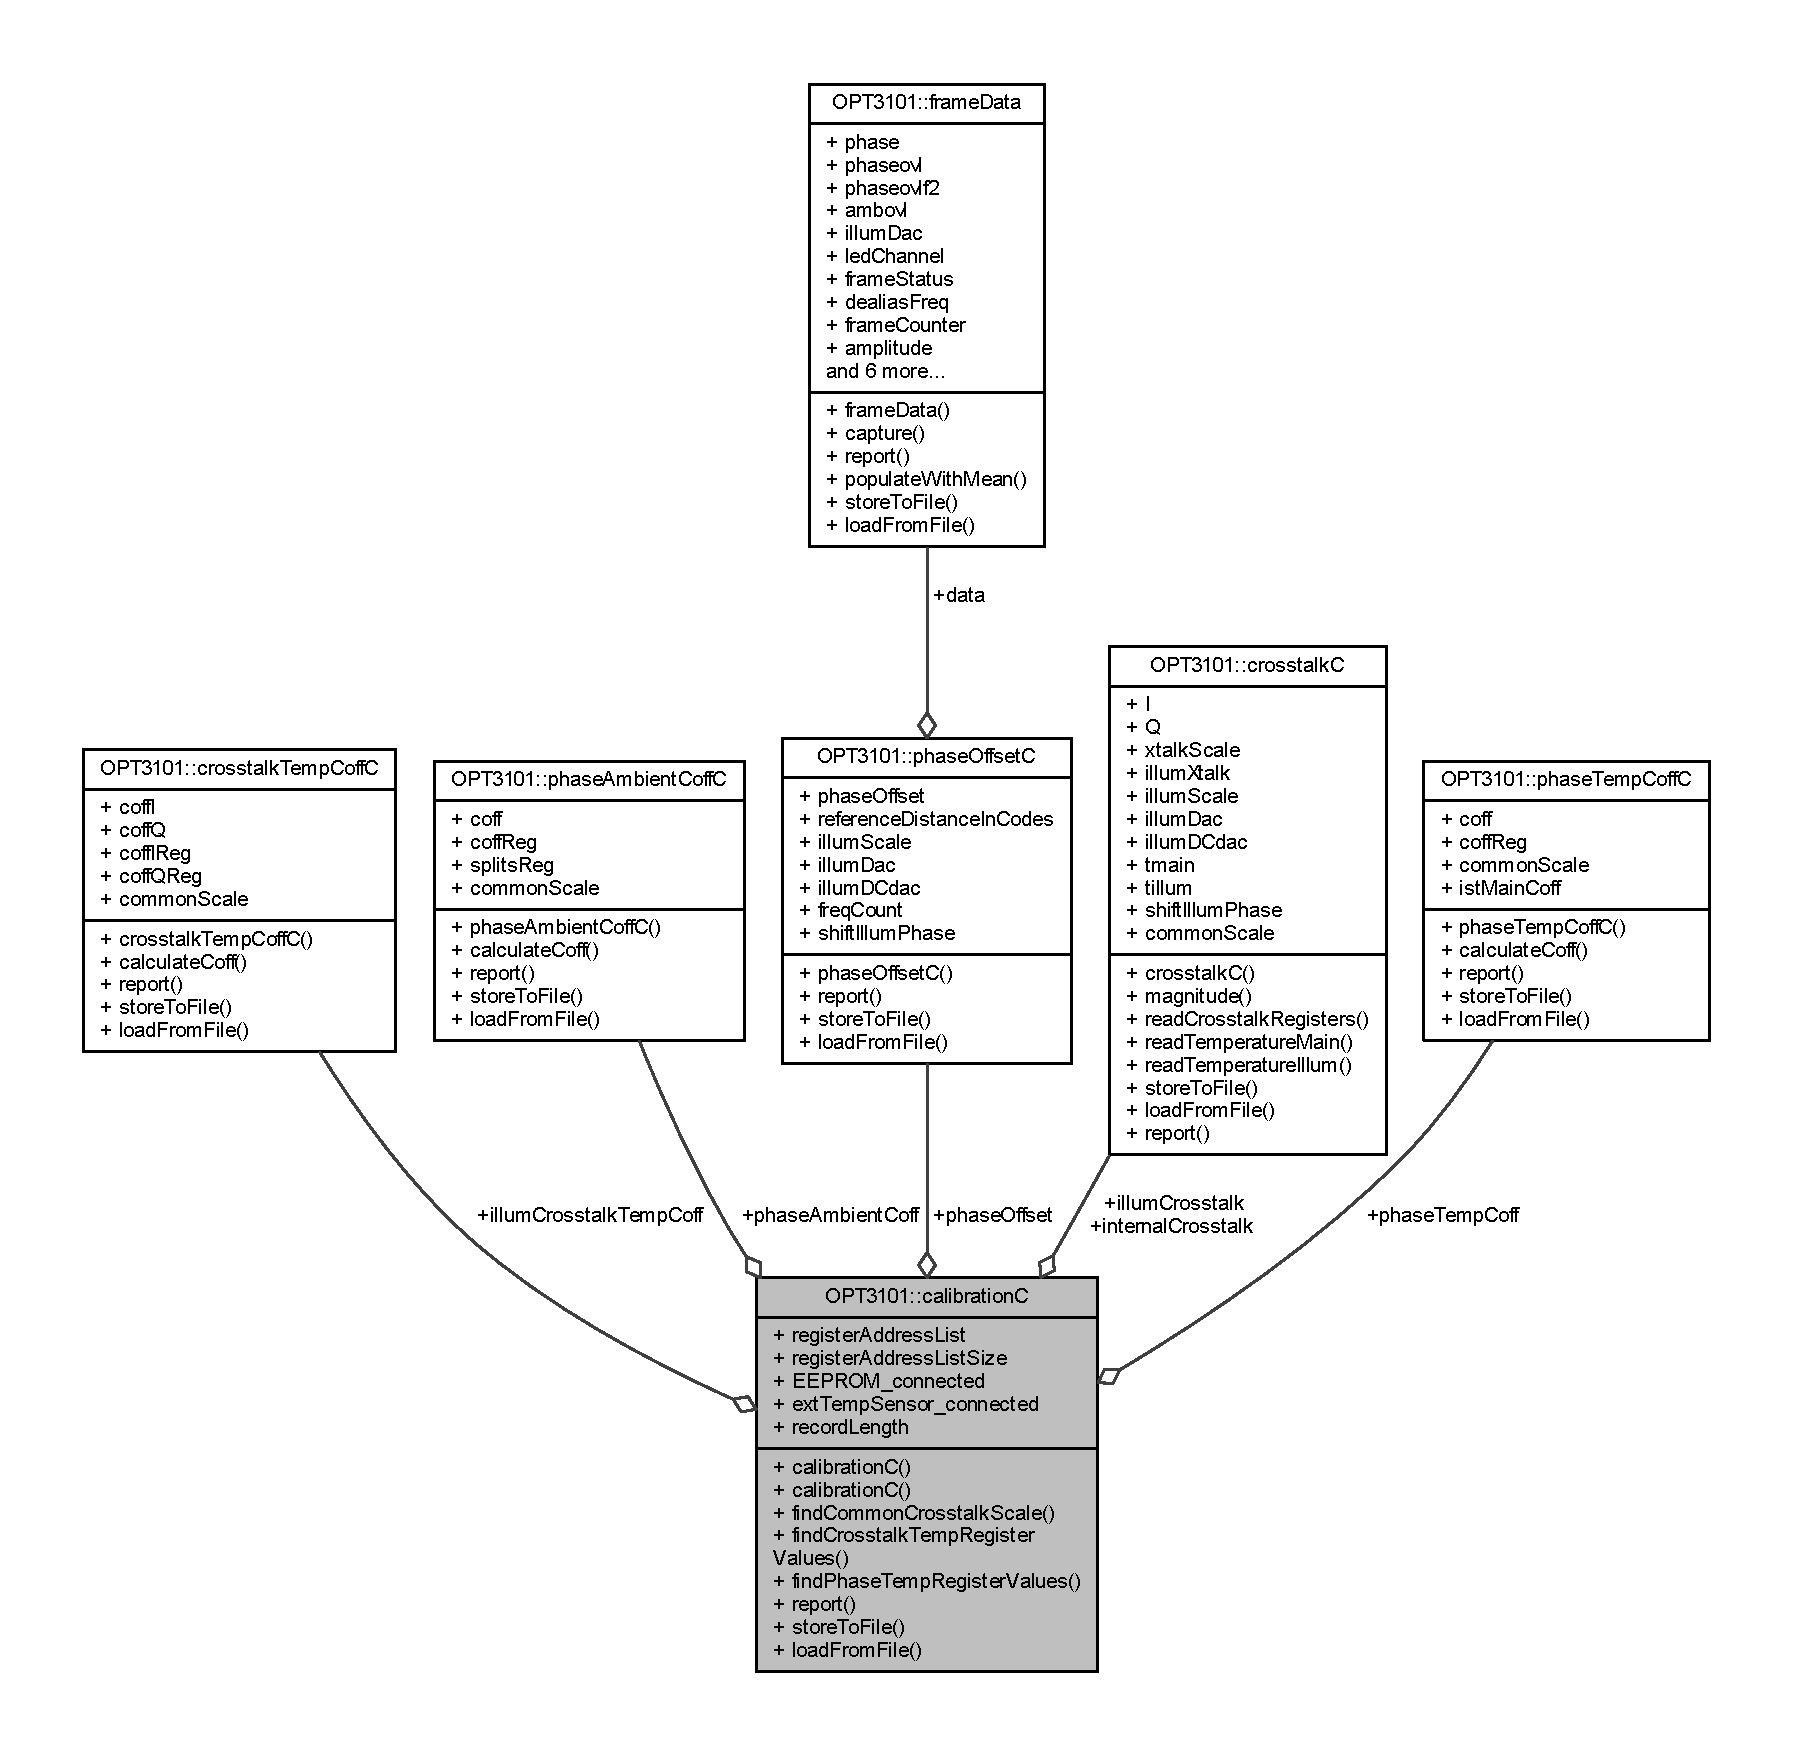
\includegraphics[width=350pt]{class_o_p_t3101_1_1calibration_c__coll__graph}
\end{center}
\end{figure}
\subsection*{Public Member Functions}
\begin{DoxyCompactItemize}
\item 
\mbox{\hyperlink{class_o_p_t3101_1_1calibration_c_a84e3f1b924cf7f677977e36663ddad7a}{calibrationC}} (bool dummy\+Flag)
\begin{DoxyCompactList}\small\item\em Dummy function for documentation This function is to just document the functionality of the constructor. \end{DoxyCompactList}\item 
\mbox{\hyperlink{class_o_p_t3101_1_1calibration_c_adaa42643a7b88087e4909f7017a85ef4}{calibrationC}} ()
\begin{DoxyCompactList}\small\item\em Constructor for class \mbox{\hyperlink{class_o_p_t3101_1_1calibration_c}{O\+P\+T3101\+::calibrationC}} Constructor definition for which comes from the \mbox{\hyperlink{namespace_o_p_t3101}{O\+P\+T3101}} configurator tool. Allocates memory for all the calibration coefficient classes. Since the actual allocation depends on the configuration of the system, this is generated by the configurator tool. \end{DoxyCompactList}\item 
void \mbox{\hyperlink{class_o_p_t3101_1_1calibration_c_ae2c3f2786e65315d817b8953380e33b6}{find\+Common\+Crosstalk\+Scale}} (\mbox{\hyperlink{class_o_p_t3101_1_1crosstalk_c}{crosstalkC}} $\ast$illum\+Xtalk, uint8\+\_\+t size)
\begin{DoxyCompactList}\small\item\em Finds common crosstalk scale coff to be applied \mbox{\hyperlink{namespace_o_p_t3101}{O\+P\+T3101}} system could consist of multiple TX configuration operating together, switching between each other configurations. In such cases more than 1 illum crosstalk compensation registers needs to be applied however \mbox{\hyperlink{namespace_o_p_t3101}{O\+P\+T3101}} has only one common scale which this method computes. \end{DoxyCompactList}\item 
void \mbox{\hyperlink{class_o_p_t3101_1_1calibration_c_ac133c41d60c71559a224a86bc3e62c3a}{find\+Crosstalk\+Temp\+Register\+Values}} (\mbox{\hyperlink{class_o_p_t3101_1_1crosstalk_temp_coff_c}{crosstalk\+Temp\+CoffC}} $\ast$illum\+Xtalk\+Coff, uint8\+\_\+t size, \mbox{\hyperlink{class_o_p_t3101_1_1crosstalk_c}{crosstalkC}} $\ast$illum\+Xtalk)
\begin{DoxyCompactList}\small\item\em Calculates crosstalk temp coefficient registers from floating point precision coefficients \mbox{\hyperlink{namespace_o_p_t3101}{O\+P\+T3101}} system could consist of multiple TX configuration operating together, switching between each other configurations. In such cases more than 1 illum crosstalk temperature compensation registers needs to be applied. \mbox{\hyperlink{namespace_o_p_t3101}{O\+P\+T3101}} has only one common scale which this method computes along with the registers that need to be written to compensate these effects. \end{DoxyCompactList}\item 
void \mbox{\hyperlink{class_o_p_t3101_1_1calibration_c_a5ca75c8e4d7818a90cacc0471522b365}{find\+Phase\+Temp\+Register\+Values}} (\mbox{\hyperlink{class_o_p_t3101_1_1phase_temp_coff_c}{phase\+Temp\+CoffC}} $\ast$\mbox{\hyperlink{class_o_p_t3101_1_1calibration_c_a277a7bbf506f5f5181719311d10bc610}{phase\+Temp\+Coff}}, uint8\+\_\+t size, uint16\+\_\+t freq\+Count)
\begin{DoxyCompactList}\small\item\em calculates the phase temp coff register values from the floating point coff \mbox{\hyperlink{namespace_o_p_t3101}{O\+P\+T3101}} system could consist of multiple TX configuration operating together, switching between each other configurations. In such cases more than 1 phase temperature compensation registers needs to be applied. \mbox{\hyperlink{namespace_o_p_t3101}{O\+P\+T3101}} has only one common scale which this method computes along with the registers that need to be written to compensate these effects. \end{DoxyCompactList}\item 
void \mbox{\hyperlink{class_o_p_t3101_1_1calibration_c_a092218b4999bced567ec60d147e66caa}{report}} ()
\begin{DoxyCompactList}\small\item\em reports members of the instance Print the members of the class instance on screen \end{DoxyCompactList}\item 
void \mbox{\hyperlink{class_o_p_t3101_1_1calibration_c_a3a8c57f480444c89fc855f7c90d4d81c}{store\+To\+File}} (char $\ast$file\+Name)
\begin{DoxyCompactList}\small\item\em saves phase temp coff values to file This methods saves the phase temp coff values to a non-\/volatile memory. Storage/\+Restoration to/from non-\/volatile memory is important for factory calibration \end{DoxyCompactList}\item 
void \mbox{\hyperlink{class_o_p_t3101_1_1calibration_c_aa84c53e8568557e5f12819c6736d5b37}{load\+From\+File}} (char $\ast$file\+Name)
\begin{DoxyCompactList}\small\item\em load phase temp coff values from file This methods loads the phase temp coff values to a non-\/volatile memory. Storage/\+Restoration to/from non-\/volatile memory is important for factory calibration \end{DoxyCompactList}\end{DoxyCompactItemize}
\subsection*{Public Attributes}
\begin{DoxyCompactItemize}
\item 
\mbox{\hyperlink{class_o_p_t3101_1_1crosstalk_c}{crosstalkC}} $\ast$ \mbox{\hyperlink{class_o_p_t3101_1_1calibration_c_a4df5b876541e9b33eadf6290fe08b7e5}{internal\+Crosstalk}}
\begin{DoxyCompactList}\small\item\em Pointer to analyze and store internal crosstalk class \mbox{\hyperlink{class_o_p_t3101_1_1crosstalk_c}{O\+P\+T3101\+::crosstalkC}}. \end{DoxyCompactList}\item 
\mbox{\hyperlink{class_o_p_t3101_1_1crosstalk_c}{crosstalkC}} $\ast$ \mbox{\hyperlink{class_o_p_t3101_1_1calibration_c_ac09121c7057093506de63d6e2ea3a4b7}{illum\+Crosstalk}}
\begin{DoxyCompactList}\small\item\em Pointer to analyze and store illumination crosstalk class \mbox{\hyperlink{class_o_p_t3101_1_1crosstalk_c}{O\+P\+T3101\+::crosstalkC}}. \end{DoxyCompactList}\item 
\mbox{\hyperlink{class_o_p_t3101_1_1phase_offset_c}{phase\+OffsetC}} $\ast$ \mbox{\hyperlink{class_o_p_t3101_1_1calibration_c_a06f6a097057b9ed8f4914f4027d709c1}{phase\+Offset}}
\begin{DoxyCompactList}\small\item\em Pointer to analyze and store phase offset class \mbox{\hyperlink{class_o_p_t3101_1_1phase_offset_c}{O\+P\+T3101\+::phase\+OffsetC}}. \end{DoxyCompactList}\item 
\mbox{\hyperlink{class_o_p_t3101_1_1crosstalk_temp_coff_c}{crosstalk\+Temp\+CoffC}} $\ast$ \mbox{\hyperlink{class_o_p_t3101_1_1calibration_c_ac7bcc22317965bb378479fb016c20d3c}{illum\+Crosstalk\+Temp\+Coff}}
\begin{DoxyCompactList}\small\item\em Pointer to analyze and store crosstalk temperature coefficients \mbox{\hyperlink{class_o_p_t3101_1_1crosstalk_temp_coff_c}{O\+P\+T3101\+::crosstalk\+Temp\+CoffC}}. \end{DoxyCompactList}\item 
\mbox{\hyperlink{class_o_p_t3101_1_1phase_temp_coff_c}{phase\+Temp\+CoffC}} $\ast$ \mbox{\hyperlink{class_o_p_t3101_1_1calibration_c_a277a7bbf506f5f5181719311d10bc610}{phase\+Temp\+Coff}}
\begin{DoxyCompactList}\small\item\em Pointer to analyze and store phase temperature coefficients \mbox{\hyperlink{class_o_p_t3101_1_1phase_temp_coff_c}{O\+P\+T3101\+::phase\+Temp\+CoffC}}. \end{DoxyCompactList}\item 
\mbox{\hyperlink{class_o_p_t3101_1_1phase_ambient_coff_c}{phase\+Ambient\+CoffC}} $\ast$ \mbox{\hyperlink{class_o_p_t3101_1_1calibration_c_ab69d912cc3cad353abeb73d7a95b7428}{phase\+Ambient\+Coff}}
\begin{DoxyCompactList}\small\item\em Pointer to analyze and store phase ambient coefficients \mbox{\hyperlink{class_o_p_t3101_1_1phase_ambient_coff_c}{O\+P\+T3101\+::phase\+Ambient\+CoffC}}. \end{DoxyCompactList}\item 
uint8\+\_\+t $\ast$ \mbox{\hyperlink{class_o_p_t3101_1_1calibration_c_a8ddd81159778cc987557c9b4920d5b57}{register\+Address\+List}}
\begin{DoxyCompactList}\small\item\em List of \mbox{\hyperlink{class_o_p_t3101_1_1registers}{O\+P\+T3101\+::registers}} address which needs to be stored as calibration for the system. \end{DoxyCompactList}\item 
uint8\+\_\+t \mbox{\hyperlink{class_o_p_t3101_1_1calibration_c_a5331ffae8b40e63d277b907a6bf84aa3}{register\+Address\+List\+Size}}
\begin{DoxyCompactList}\small\item\em Number of \mbox{\hyperlink{class_o_p_t3101_1_1registers}{O\+P\+T3101\+::registers}} address that need to be stores as calibration for the system. \end{DoxyCompactList}\item 
bool \mbox{\hyperlink{class_o_p_t3101_1_1calibration_c_ac56e02e52f84fb4a601b0104e0c6b607}{E\+E\+P\+R\+O\+M\+\_\+connected}}
\begin{DoxyCompactList}\small\item\em Flag to specify if E\+E\+P\+R\+OM is connected to the \mbox{\hyperlink{namespace_o_p_t3101}{O\+P\+T3101}} device. \end{DoxyCompactList}\item 
bool \mbox{\hyperlink{class_o_p_t3101_1_1calibration_c_a703a4667679ca3cfd19801908cdbf153}{ext\+Temp\+Sensor\+\_\+connected}}
\begin{DoxyCompactList}\small\item\em Flag to specify if external temperature sensor is connected to the \mbox{\hyperlink{namespace_o_p_t3101}{O\+P\+T3101}} device. \end{DoxyCompactList}\item 
uint8\+\_\+t \mbox{\hyperlink{class_o_p_t3101_1_1calibration_c_a8963999e75dd21df70925512905074c0}{record\+Length}}
\begin{DoxyCompactList}\small\item\em Specifies the length of records to be stored for calibration configurations. This is set be \mbox{\hyperlink{namespace_o_p_t3101}{O\+P\+T3101}} configurator tool. \end{DoxyCompactList}\end{DoxyCompactItemize}
\subsection*{Friends}
\begin{DoxyCompactItemize}
\item 
std\+::ostream \& \mbox{\hyperlink{class_o_p_t3101_1_1calibration_c_ad4bd440df02467a0bbb3f15f07a27e2b}{operator$<$$<$}} (std\+::ostream \&os, const \mbox{\hyperlink{class_o_p_t3101_1_1calibration_c}{calibrationC}} $\ast$data)
\begin{DoxyCompactList}\small\item\em Operator overload to store class contents to a file Casts all the class members for file storage. \end{DoxyCompactList}\item 
std\+::istream \& \mbox{\hyperlink{class_o_p_t3101_1_1calibration_c_a06e5b13fed9266160b9ed9f43d17bca8}{operator$>$$>$}} (std\+::istream \&is, \mbox{\hyperlink{class_o_p_t3101_1_1calibration_c}{calibrationC}} $\ast$data)
\begin{DoxyCompactList}\small\item\em Operator overload to load class contents to from a file Retreives all the class members from a stored file. \end{DoxyCompactList}\end{DoxyCompactItemize}


\subsection{Detailed Description}
Class contains the instances of classes required during \mbox{\hyperlink{namespace_o_p_t3101}{O\+P\+T3101}} calibration. 

\mbox{\hyperlink{namespace_o_p_t3101}{O\+P\+T3101}} systems require various calibrations for accurate measurement. During the calibration process there are several coefficients which needs to be measured and analyzed. Although the calibration settings can be stored as register settings, they would not be very meaning full to understand and analyze. This class acts as an intermediate translator to measure, store and calibration values. The class also invokes methods to convert the calibration coefficients to register settings to load to the device. There are several members of this class where more than 1 instances of those members are required. The class only contain pointers for these coefficient classes. The constructor definition of this class is generated by \mbox{\hyperlink{namespace_o_p_t3101}{O\+P\+T3101}} configurator tool. The file generated by the tool can be directly imported to this project for a complete operation S\+DK. 

\subsection{Constructor \& Destructor Documentation}
\mbox{\Hypertarget{class_o_p_t3101_1_1calibration_c_a84e3f1b924cf7f677977e36663ddad7a}\label{class_o_p_t3101_1_1calibration_c_a84e3f1b924cf7f677977e36663ddad7a}} 
\index{O\+P\+T3101\+::calibrationC@{O\+P\+T3101\+::calibrationC}!calibrationC@{calibrationC}}
\index{calibrationC@{calibrationC}!O\+P\+T3101\+::calibrationC@{O\+P\+T3101\+::calibrationC}}
\subsubsection{\texorpdfstring{calibration\+C()}{calibrationC()}\hspace{0.1cm}{\footnotesize\ttfamily [1/2]}}
{\footnotesize\ttfamily O\+P\+T3101\+::calibration\+C\+::calibrationC (\begin{DoxyParamCaption}\item[{bool}]{dummy\+Flag }\end{DoxyParamCaption})}



Dummy function for documentation This function is to just document the functionality of the constructor. 

\begin{DoxyReturn}{Returns}
Nothing; 
\end{DoxyReturn}
{\bfseries Algorithm of the method is as follows}
\begin{DoxyItemize}
\item Allocates memory for \mbox{\hyperlink{class_o_p_t3101_1_1calibration_c_a4df5b876541e9b33eadf6290fe08b7e5}{O\+P\+T3101\+::calibration\+C\+::internal\+Crosstalk}} size based on system configuration
\item Allocates memory for \mbox{\hyperlink{class_o_p_t3101_1_1calibration_c_ac09121c7057093506de63d6e2ea3a4b7}{O\+P\+T3101\+::calibration\+C\+::illum\+Crosstalk}} size based on system configuration
\item Allocates memory for \mbox{\hyperlink{class_o_p_t3101_1_1calibration_c_a06f6a097057b9ed8f4914f4027d709c1}{O\+P\+T3101\+::calibration\+C\+::phase\+Offset}} size based on system configuration
\item Allocates memory for \mbox{\hyperlink{class_o_p_t3101_1_1calibration_c_ac7bcc22317965bb378479fb016c20d3c}{O\+P\+T3101\+::calibration\+C\+::illum\+Crosstalk\+Temp\+Coff}} size based on system configuration
\item Allocates memory for \mbox{\hyperlink{class_o_p_t3101_1_1calibration_c_a277a7bbf506f5f5181719311d10bc610}{O\+P\+T3101\+::calibration\+C\+::phase\+Temp\+Coff}} size based on system configuration
\item Allocates memory for \mbox{\hyperlink{class_o_p_t3101_1_1calibration_c_ab69d912cc3cad353abeb73d7a95b7428}{O\+P\+T3101\+::calibration\+C\+::phase\+Ambient\+Coff}} size based on system configuration
\item Sets the member \mbox{\hyperlink{class_o_p_t3101_1_1calibration_c_a5331ffae8b40e63d277b907a6bf84aa3}{O\+P\+T3101\+::calibration\+C\+::register\+Address\+List\+Size}} based on number of calibration registers requires
\item Allocates memory for \mbox{\hyperlink{class_o_p_t3101_1_1calibration_c_a8ddd81159778cc987557c9b4920d5b57}{O\+P\+T3101\+::calibration\+C\+::register\+Address\+List}} based on \mbox{\hyperlink{class_o_p_t3101_1_1calibration_c_a5331ffae8b40e63d277b907a6bf84aa3}{O\+P\+T3101\+::calibration\+C\+::register\+Address\+List\+Size}}
\item Sets up the flag \mbox{\hyperlink{class_o_p_t3101_1_1calibration_c_ac56e02e52f84fb4a601b0104e0c6b607}{O\+P\+T3101\+::calibration\+C\+::\+E\+E\+P\+R\+O\+M\+\_\+connected}} based on configuration
\item Sets up the flag \mbox{\hyperlink{class_o_p_t3101_1_1calibration_c_a703a4667679ca3cfd19801908cdbf153}{O\+P\+T3101\+::calibration\+C\+::ext\+Temp\+Sensor\+\_\+connected}} based on configuration 
\end{DoxyItemize}\mbox{\Hypertarget{class_o_p_t3101_1_1calibration_c_adaa42643a7b88087e4909f7017a85ef4}\label{class_o_p_t3101_1_1calibration_c_adaa42643a7b88087e4909f7017a85ef4}} 
\index{O\+P\+T3101\+::calibrationC@{O\+P\+T3101\+::calibrationC}!calibrationC@{calibrationC}}
\index{calibrationC@{calibrationC}!O\+P\+T3101\+::calibrationC@{O\+P\+T3101\+::calibrationC}}
\subsubsection{\texorpdfstring{calibration\+C()}{calibrationC()}\hspace{0.1cm}{\footnotesize\ttfamily [2/2]}}
{\footnotesize\ttfamily O\+P\+T3101\+::calibration\+C\+::calibrationC (\begin{DoxyParamCaption}{ }\end{DoxyParamCaption})}



Constructor for class \mbox{\hyperlink{class_o_p_t3101_1_1calibration_c}{O\+P\+T3101\+::calibrationC}} Constructor definition for which comes from the \mbox{\hyperlink{namespace_o_p_t3101}{O\+P\+T3101}} configurator tool. Allocates memory for all the calibration coefficient classes. Since the actual allocation depends on the configuration of the system, this is generated by the configurator tool. 



\subsection{Member Function Documentation}
\mbox{\Hypertarget{class_o_p_t3101_1_1calibration_c_ae2c3f2786e65315d817b8953380e33b6}\label{class_o_p_t3101_1_1calibration_c_ae2c3f2786e65315d817b8953380e33b6}} 
\index{O\+P\+T3101\+::calibrationC@{O\+P\+T3101\+::calibrationC}!find\+Common\+Crosstalk\+Scale@{find\+Common\+Crosstalk\+Scale}}
\index{find\+Common\+Crosstalk\+Scale@{find\+Common\+Crosstalk\+Scale}!O\+P\+T3101\+::calibrationC@{O\+P\+T3101\+::calibrationC}}
\subsubsection{\texorpdfstring{find\+Common\+Crosstalk\+Scale()}{findCommonCrosstalkScale()}}
{\footnotesize\ttfamily void O\+P\+T3101\+::calibration\+C\+::find\+Common\+Crosstalk\+Scale (\begin{DoxyParamCaption}\item[{\mbox{\hyperlink{class_o_p_t3101_1_1crosstalk_c}{O\+P\+T3101\+::crosstalkC}} $\ast$}]{illum\+Xtalk,  }\item[{uint8\+\_\+t}]{size }\end{DoxyParamCaption})}



Finds common crosstalk scale coff to be applied \mbox{\hyperlink{namespace_o_p_t3101}{O\+P\+T3101}} system could consist of multiple TX configuration operating together, switching between each other configurations. In such cases more than 1 illum crosstalk compensation registers needs to be applied however \mbox{\hyperlink{namespace_o_p_t3101}{O\+P\+T3101}} has only one common scale which this method computes. 


\begin{DoxyParams}[1]{Parameters}
\mbox{\tt in,out}  & {\em illum\+Xtalk;} & illum\+Xtalk is pointer to \mbox{\hyperlink{class_o_p_t3101_1_1crosstalk_c}{O\+P\+T3101\+::crosstalkC}} class which contains the list of crosstalk instances for which the common coefficient needs to be calculated. \\
\hline
\mbox{\tt in}  & {\em size;} & size represents the number of \mbox{\hyperlink{class_o_p_t3101_1_1crosstalk_c}{O\+P\+T3101\+::crosstalkC}} instances available in the illum\+Xtalk pointer argument \\
\hline
\end{DoxyParams}
\begin{DoxyReturn}{Returns}
Nothing; 
\end{DoxyReturn}
{\bfseries Algorithm of the method is as follows}


\begin{DoxyItemize}
\item Finds the largest scale what will fit all the input \mbox{\hyperlink{class_o_p_t3101_1_1crosstalk_c}{O\+P\+T3101\+::crosstalkC}} arguments
\item Assigns the identified max\+Scale to all the input argument illum Crosstalk pointers \mbox{\hyperlink{class_o_p_t3101_1_1crosstalk_c}{O\+P\+T3101\+::crosstalkC}} 
\end{DoxyItemize}\mbox{\Hypertarget{class_o_p_t3101_1_1calibration_c_ac133c41d60c71559a224a86bc3e62c3a}\label{class_o_p_t3101_1_1calibration_c_ac133c41d60c71559a224a86bc3e62c3a}} 
\index{O\+P\+T3101\+::calibrationC@{O\+P\+T3101\+::calibrationC}!find\+Crosstalk\+Temp\+Register\+Values@{find\+Crosstalk\+Temp\+Register\+Values}}
\index{find\+Crosstalk\+Temp\+Register\+Values@{find\+Crosstalk\+Temp\+Register\+Values}!O\+P\+T3101\+::calibrationC@{O\+P\+T3101\+::calibrationC}}
\subsubsection{\texorpdfstring{find\+Crosstalk\+Temp\+Register\+Values()}{findCrosstalkTempRegisterValues()}}
{\footnotesize\ttfamily void O\+P\+T3101\+::calibration\+C\+::find\+Crosstalk\+Temp\+Register\+Values (\begin{DoxyParamCaption}\item[{\mbox{\hyperlink{class_o_p_t3101_1_1crosstalk_temp_coff_c}{O\+P\+T3101\+::crosstalk\+Temp\+CoffC}} $\ast$}]{illum\+Xtalk\+Coff,  }\item[{uint8\+\_\+t}]{size,  }\item[{\mbox{\hyperlink{class_o_p_t3101_1_1crosstalk_c}{O\+P\+T3101\+::crosstalkC}} $\ast$}]{illum\+Xtalk }\end{DoxyParamCaption})}



Calculates crosstalk temp coefficient registers from floating point precision coefficients \mbox{\hyperlink{namespace_o_p_t3101}{O\+P\+T3101}} system could consist of multiple TX configuration operating together, switching between each other configurations. In such cases more than 1 illum crosstalk temperature compensation registers needs to be applied. \mbox{\hyperlink{namespace_o_p_t3101}{O\+P\+T3101}} has only one common scale which this method computes along with the registers that need to be written to compensate these effects. 


\begin{DoxyParams}[1]{Parameters}
\mbox{\tt in,out}  & {\em illum\+Xtalk\+Coff;} & illum\+Xtalk\+Coff is pointer to \mbox{\hyperlink{class_o_p_t3101_1_1crosstalk_temp_coff_c}{O\+P\+T3101\+::crosstalk\+Temp\+CoffC}} class which contains the list of crosstalk temp coefficients for which the register values needs to be calculated. \\
\hline
\mbox{\tt in}  & {\em size;} & size represents the number of \mbox{\hyperlink{class_o_p_t3101_1_1crosstalk_c}{O\+P\+T3101\+::crosstalkC}} instances available in the illum\+Xtalk pointer argument \\
\hline
\mbox{\tt in}  & {\em illum\+Xtalk;} & illum\+Xtalk is pointer to \mbox{\hyperlink{class_o_p_t3101_1_1crosstalk_temp_coff_c}{O\+P\+T3101\+::crosstalk\+Temp\+CoffC}} class which contains the list of crosstalk instances for which the common coefficient needs to be calculated. This is mainly required to scale the crosstalk values with magnitude \\
\hline
\end{DoxyParams}
\begin{DoxyReturn}{Returns}
Nothing; 
\end{DoxyReturn}
\mbox{\Hypertarget{class_o_p_t3101_1_1calibration_c_a5ca75c8e4d7818a90cacc0471522b365}\label{class_o_p_t3101_1_1calibration_c_a5ca75c8e4d7818a90cacc0471522b365}} 
\index{O\+P\+T3101\+::calibrationC@{O\+P\+T3101\+::calibrationC}!find\+Phase\+Temp\+Register\+Values@{find\+Phase\+Temp\+Register\+Values}}
\index{find\+Phase\+Temp\+Register\+Values@{find\+Phase\+Temp\+Register\+Values}!O\+P\+T3101\+::calibrationC@{O\+P\+T3101\+::calibrationC}}
\subsubsection{\texorpdfstring{find\+Phase\+Temp\+Register\+Values()}{findPhaseTempRegisterValues()}}
{\footnotesize\ttfamily void O\+P\+T3101\+::calibration\+C\+::find\+Phase\+Temp\+Register\+Values (\begin{DoxyParamCaption}\item[{\mbox{\hyperlink{class_o_p_t3101_1_1phase_temp_coff_c}{O\+P\+T3101\+::phase\+Temp\+CoffC}} $\ast$}]{phase\+Temp\+Coff,  }\item[{uint8\+\_\+t}]{size,  }\item[{uint16\+\_\+t}]{freq\+Count }\end{DoxyParamCaption})}



calculates the phase temp coff register values from the floating point coff \mbox{\hyperlink{namespace_o_p_t3101}{O\+P\+T3101}} system could consist of multiple TX configuration operating together, switching between each other configurations. In such cases more than 1 phase temperature compensation registers needs to be applied. \mbox{\hyperlink{namespace_o_p_t3101}{O\+P\+T3101}} has only one common scale which this method computes along with the registers that need to be written to compensate these effects. 


\begin{DoxyParams}[1]{Parameters}
\mbox{\tt in,out}  & {\em phase\+Temp\+Coff;} & phase\+Temp\+Coff is pointer to \mbox{\hyperlink{class_o_p_t3101_1_1phase_temp_coff_c}{O\+P\+T3101\+::phase\+Temp\+CoffC}} class which contains the list of phase temp coefficients for which the register values needs to be calculated. \\
\hline
\mbox{\tt in}  & {\em size;} & size represents the number of \mbox{\hyperlink{class_o_p_t3101_1_1phase_temp_coff_c}{O\+P\+T3101\+::phase\+Temp\+CoffC}} instances available in the phase\+Temp\+Coff pointer argument \\
\hline
\mbox{\tt in}  & {\em freq\+Count;} & freq\+Count is frequency count register read from \mbox{\hyperlink{class_o_p_t3101_1_1registers_a0d343738560c0bc418f34b458735a811}{O\+P\+T3101\+::registers\+::freq\+\_\+count\+\_\+read\+\_\+reg}}. This is used to scale the coefficients accordingly \\
\hline
\end{DoxyParams}
\begin{DoxyReturn}{Returns}
Nothing; 
\end{DoxyReturn}
{\bfseries Algorithm of the method is as follows}


\begin{DoxyItemize}
\item Identifies max of absolute of \mbox{\hyperlink{class_o_p_t3101_1_1phase_temp_coff_c_ade7d29c7cac1e63af7910eec0ec38043}{O\+P\+T3101\+::phase\+Temp\+Coff\+C\+::coff}} values ~\newline
~\newline
~\newline

\item scales the max coefficient with input frequency\+Count ~\newline
~\newline

\item Finds a \mbox{\hyperlink{class_o_p_t3101_1_1phase_temp_coff_c_a0f7646d71d058bc5354ac8f14270fcf3}{O\+P\+T3101\+::phase\+Temp\+Coff\+C\+::common\+Scale}} which can fit the \mbox{\hyperlink{class_o_p_t3101_1_1phase_temp_coff_c_ade7d29c7cac1e63af7910eec0ec38043}{O\+P\+T3101\+::phase\+Temp\+Coff\+C\+::coff}} to 12 bit registers
\item Finds \mbox{\hyperlink{class_o_p_t3101_1_1phase_temp_coff_c_a69e1782e097ce7ab761e4e55b5206f2e}{O\+P\+T3101\+::phase\+Temp\+Coff\+C\+::coff\+Reg}} values (12 bit register values) based on \mbox{\hyperlink{class_o_p_t3101_1_1phase_temp_coff_c_ade7d29c7cac1e63af7910eec0ec38043}{O\+P\+T3101\+::phase\+Temp\+Coff\+C\+::coff}} and \mbox{\hyperlink{class_o_p_t3101_1_1phase_temp_coff_c_a0f7646d71d058bc5354ac8f14270fcf3}{O\+P\+T3101\+::phase\+Temp\+Coff\+C\+::common\+Scale}} 
\end{DoxyItemize}\mbox{\Hypertarget{class_o_p_t3101_1_1calibration_c_aa84c53e8568557e5f12819c6736d5b37}\label{class_o_p_t3101_1_1calibration_c_aa84c53e8568557e5f12819c6736d5b37}} 
\index{O\+P\+T3101\+::calibrationC@{O\+P\+T3101\+::calibrationC}!load\+From\+File@{load\+From\+File}}
\index{load\+From\+File@{load\+From\+File}!O\+P\+T3101\+::calibrationC@{O\+P\+T3101\+::calibrationC}}
\subsubsection{\texorpdfstring{load\+From\+File()}{loadFromFile()}}
{\footnotesize\ttfamily void O\+P\+T3101\+::calibration\+C\+::load\+From\+File (\begin{DoxyParamCaption}\item[{char $\ast$}]{file\+Name }\end{DoxyParamCaption})}



load phase temp coff values from file This methods loads the phase temp coff values to a non-\/volatile memory. Storage/\+Restoration to/from non-\/volatile memory is important for factory calibration 


\begin{DoxyParams}[1]{Parameters}
\mbox{\tt in}  & {\em file\+Name;} & Path and name of the file from where to load \\
\hline
\end{DoxyParams}
\begin{DoxyReturn}{Returns}
Nothing; 
\end{DoxyReturn}
{\bfseries Algorithm of the method is as follows}


\begin{DoxyItemize}
\item User needs to implement file load/restore based on host. 
\end{DoxyItemize}\mbox{\Hypertarget{class_o_p_t3101_1_1calibration_c_a092218b4999bced567ec60d147e66caa}\label{class_o_p_t3101_1_1calibration_c_a092218b4999bced567ec60d147e66caa}} 
\index{O\+P\+T3101\+::calibrationC@{O\+P\+T3101\+::calibrationC}!report@{report}}
\index{report@{report}!O\+P\+T3101\+::calibrationC@{O\+P\+T3101\+::calibrationC}}
\subsubsection{\texorpdfstring{report()}{report()}}
{\footnotesize\ttfamily void O\+P\+T3101\+::calibration\+C\+::report (\begin{DoxyParamCaption}{ }\end{DoxyParamCaption})}



reports members of the instance Print the members of the class instance on screen 

\begin{DoxyReturn}{Returns}
Nothing; 
\end{DoxyReturn}
{\bfseries Algorithm of the method is as follows}


\begin{DoxyItemize}
\item Prints all the members and values of members on screen. 
\end{DoxyItemize}\mbox{\Hypertarget{class_o_p_t3101_1_1calibration_c_a3a8c57f480444c89fc855f7c90d4d81c}\label{class_o_p_t3101_1_1calibration_c_a3a8c57f480444c89fc855f7c90d4d81c}} 
\index{O\+P\+T3101\+::calibrationC@{O\+P\+T3101\+::calibrationC}!store\+To\+File@{store\+To\+File}}
\index{store\+To\+File@{store\+To\+File}!O\+P\+T3101\+::calibrationC@{O\+P\+T3101\+::calibrationC}}
\subsubsection{\texorpdfstring{store\+To\+File()}{storeToFile()}}
{\footnotesize\ttfamily void O\+P\+T3101\+::calibration\+C\+::store\+To\+File (\begin{DoxyParamCaption}\item[{char $\ast$}]{file\+Name }\end{DoxyParamCaption})}



saves phase temp coff values to file This methods saves the phase temp coff values to a non-\/volatile memory. Storage/\+Restoration to/from non-\/volatile memory is important for factory calibration 


\begin{DoxyParams}[1]{Parameters}
\mbox{\tt in}  & {\em file\+Name;} & Path and name of the file to store \\
\hline
\end{DoxyParams}
\begin{DoxyReturn}{Returns}
Nothing; 
\end{DoxyReturn}
{\bfseries Algorithm of the method is as follows}


\begin{DoxyItemize}
\item User needs to implement file storage based on host. 
\end{DoxyItemize}

\subsection{Friends And Related Function Documentation}
\mbox{\Hypertarget{class_o_p_t3101_1_1calibration_c_ad4bd440df02467a0bbb3f15f07a27e2b}\label{class_o_p_t3101_1_1calibration_c_ad4bd440df02467a0bbb3f15f07a27e2b}} 
\index{O\+P\+T3101\+::calibrationC@{O\+P\+T3101\+::calibrationC}!operator$<$$<$@{operator$<$$<$}}
\index{operator$<$$<$@{operator$<$$<$}!O\+P\+T3101\+::calibrationC@{O\+P\+T3101\+::calibrationC}}
\subsubsection{\texorpdfstring{operator$<$$<$}{operator<<}}
{\footnotesize\ttfamily std\+::ostream\& operator$<$$<$ (\begin{DoxyParamCaption}\item[{std\+::ostream \&}]{os,  }\item[{const \mbox{\hyperlink{class_o_p_t3101_1_1calibration_c}{calibrationC}} $\ast$}]{data }\end{DoxyParamCaption})\hspace{0.3cm}{\ttfamily [friend]}}



Operator overload to store class contents to a file Casts all the class members for file storage. 


\begin{DoxyParams}[1]{Parameters}
\mbox{\tt out}  & {\em os;} & os is data stream to serialize data \\
\hline
\mbox{\tt in}  & {\em data;} & data is pointer to the class to be serialized and stored \\
\hline
\end{DoxyParams}
\begin{DoxyReturn}{Returns}
std\+::ostream; Serialized std\+::ostream to be written to a file 
\end{DoxyReturn}
\mbox{\Hypertarget{class_o_p_t3101_1_1calibration_c_a06e5b13fed9266160b9ed9f43d17bca8}\label{class_o_p_t3101_1_1calibration_c_a06e5b13fed9266160b9ed9f43d17bca8}} 
\index{O\+P\+T3101\+::calibrationC@{O\+P\+T3101\+::calibrationC}!operator$>$$>$@{operator$>$$>$}}
\index{operator$>$$>$@{operator$>$$>$}!O\+P\+T3101\+::calibrationC@{O\+P\+T3101\+::calibrationC}}
\subsubsection{\texorpdfstring{operator$>$$>$}{operator>>}}
{\footnotesize\ttfamily std\+::istream\& operator$>$$>$ (\begin{DoxyParamCaption}\item[{std\+::istream \&}]{is,  }\item[{\mbox{\hyperlink{class_o_p_t3101_1_1calibration_c}{calibrationC}} $\ast$}]{data }\end{DoxyParamCaption})\hspace{0.3cm}{\ttfamily [friend]}}



Operator overload to load class contents to from a file Retreives all the class members from a stored file. 


\begin{DoxyParams}[1]{Parameters}
\mbox{\tt in}  & {\em is;} & is inputstream from where the data is loaded \\
\hline
\mbox{\tt out}  & {\em data;} & data is pointer to the class to be restored \\
\hline
\end{DoxyParams}
\begin{DoxyReturn}{Returns}
std\+::istream; Serialized Input stream loaded from file 
\end{DoxyReturn}


\subsection{Member Data Documentation}
\mbox{\Hypertarget{class_o_p_t3101_1_1calibration_c_ac56e02e52f84fb4a601b0104e0c6b607}\label{class_o_p_t3101_1_1calibration_c_ac56e02e52f84fb4a601b0104e0c6b607}} 
\index{O\+P\+T3101\+::calibrationC@{O\+P\+T3101\+::calibrationC}!E\+E\+P\+R\+O\+M\+\_\+connected@{E\+E\+P\+R\+O\+M\+\_\+connected}}
\index{E\+E\+P\+R\+O\+M\+\_\+connected@{E\+E\+P\+R\+O\+M\+\_\+connected}!O\+P\+T3101\+::calibrationC@{O\+P\+T3101\+::calibrationC}}
\subsubsection{\texorpdfstring{E\+E\+P\+R\+O\+M\+\_\+connected}{EEPROM\_connected}}
{\footnotesize\ttfamily bool O\+P\+T3101\+::calibration\+C\+::\+E\+E\+P\+R\+O\+M\+\_\+connected}



Flag to specify if E\+E\+P\+R\+OM is connected to the \mbox{\hyperlink{namespace_o_p_t3101}{O\+P\+T3101}} device. 

\mbox{\Hypertarget{class_o_p_t3101_1_1calibration_c_a703a4667679ca3cfd19801908cdbf153}\label{class_o_p_t3101_1_1calibration_c_a703a4667679ca3cfd19801908cdbf153}} 
\index{O\+P\+T3101\+::calibrationC@{O\+P\+T3101\+::calibrationC}!ext\+Temp\+Sensor\+\_\+connected@{ext\+Temp\+Sensor\+\_\+connected}}
\index{ext\+Temp\+Sensor\+\_\+connected@{ext\+Temp\+Sensor\+\_\+connected}!O\+P\+T3101\+::calibrationC@{O\+P\+T3101\+::calibrationC}}
\subsubsection{\texorpdfstring{ext\+Temp\+Sensor\+\_\+connected}{extTempSensor\_connected}}
{\footnotesize\ttfamily bool O\+P\+T3101\+::calibration\+C\+::ext\+Temp\+Sensor\+\_\+connected}



Flag to specify if external temperature sensor is connected to the \mbox{\hyperlink{namespace_o_p_t3101}{O\+P\+T3101}} device. 

\mbox{\Hypertarget{class_o_p_t3101_1_1calibration_c_ac09121c7057093506de63d6e2ea3a4b7}\label{class_o_p_t3101_1_1calibration_c_ac09121c7057093506de63d6e2ea3a4b7}} 
\index{O\+P\+T3101\+::calibrationC@{O\+P\+T3101\+::calibrationC}!illum\+Crosstalk@{illum\+Crosstalk}}
\index{illum\+Crosstalk@{illum\+Crosstalk}!O\+P\+T3101\+::calibrationC@{O\+P\+T3101\+::calibrationC}}
\subsubsection{\texorpdfstring{illum\+Crosstalk}{illumCrosstalk}}
{\footnotesize\ttfamily \mbox{\hyperlink{class_o_p_t3101_1_1crosstalk_c}{crosstalkC}}$\ast$ O\+P\+T3101\+::calibration\+C\+::illum\+Crosstalk}



Pointer to analyze and store illumination crosstalk class \mbox{\hyperlink{class_o_p_t3101_1_1crosstalk_c}{O\+P\+T3101\+::crosstalkC}}. 

\mbox{\Hypertarget{class_o_p_t3101_1_1calibration_c_ac7bcc22317965bb378479fb016c20d3c}\label{class_o_p_t3101_1_1calibration_c_ac7bcc22317965bb378479fb016c20d3c}} 
\index{O\+P\+T3101\+::calibrationC@{O\+P\+T3101\+::calibrationC}!illum\+Crosstalk\+Temp\+Coff@{illum\+Crosstalk\+Temp\+Coff}}
\index{illum\+Crosstalk\+Temp\+Coff@{illum\+Crosstalk\+Temp\+Coff}!O\+P\+T3101\+::calibrationC@{O\+P\+T3101\+::calibrationC}}
\subsubsection{\texorpdfstring{illum\+Crosstalk\+Temp\+Coff}{illumCrosstalkTempCoff}}
{\footnotesize\ttfamily \mbox{\hyperlink{class_o_p_t3101_1_1crosstalk_temp_coff_c}{crosstalk\+Temp\+CoffC}}$\ast$ O\+P\+T3101\+::calibration\+C\+::illum\+Crosstalk\+Temp\+Coff}



Pointer to analyze and store crosstalk temperature coefficients \mbox{\hyperlink{class_o_p_t3101_1_1crosstalk_temp_coff_c}{O\+P\+T3101\+::crosstalk\+Temp\+CoffC}}. 

\mbox{\Hypertarget{class_o_p_t3101_1_1calibration_c_a4df5b876541e9b33eadf6290fe08b7e5}\label{class_o_p_t3101_1_1calibration_c_a4df5b876541e9b33eadf6290fe08b7e5}} 
\index{O\+P\+T3101\+::calibrationC@{O\+P\+T3101\+::calibrationC}!internal\+Crosstalk@{internal\+Crosstalk}}
\index{internal\+Crosstalk@{internal\+Crosstalk}!O\+P\+T3101\+::calibrationC@{O\+P\+T3101\+::calibrationC}}
\subsubsection{\texorpdfstring{internal\+Crosstalk}{internalCrosstalk}}
{\footnotesize\ttfamily \mbox{\hyperlink{class_o_p_t3101_1_1crosstalk_c}{crosstalkC}}$\ast$ O\+P\+T3101\+::calibration\+C\+::internal\+Crosstalk}



Pointer to analyze and store internal crosstalk class \mbox{\hyperlink{class_o_p_t3101_1_1crosstalk_c}{O\+P\+T3101\+::crosstalkC}}. 

\mbox{\Hypertarget{class_o_p_t3101_1_1calibration_c_ab69d912cc3cad353abeb73d7a95b7428}\label{class_o_p_t3101_1_1calibration_c_ab69d912cc3cad353abeb73d7a95b7428}} 
\index{O\+P\+T3101\+::calibrationC@{O\+P\+T3101\+::calibrationC}!phase\+Ambient\+Coff@{phase\+Ambient\+Coff}}
\index{phase\+Ambient\+Coff@{phase\+Ambient\+Coff}!O\+P\+T3101\+::calibrationC@{O\+P\+T3101\+::calibrationC}}
\subsubsection{\texorpdfstring{phase\+Ambient\+Coff}{phaseAmbientCoff}}
{\footnotesize\ttfamily \mbox{\hyperlink{class_o_p_t3101_1_1phase_ambient_coff_c}{phase\+Ambient\+CoffC}}$\ast$ O\+P\+T3101\+::calibration\+C\+::phase\+Ambient\+Coff}



Pointer to analyze and store phase ambient coefficients \mbox{\hyperlink{class_o_p_t3101_1_1phase_ambient_coff_c}{O\+P\+T3101\+::phase\+Ambient\+CoffC}}. 

\mbox{\Hypertarget{class_o_p_t3101_1_1calibration_c_a06f6a097057b9ed8f4914f4027d709c1}\label{class_o_p_t3101_1_1calibration_c_a06f6a097057b9ed8f4914f4027d709c1}} 
\index{O\+P\+T3101\+::calibrationC@{O\+P\+T3101\+::calibrationC}!phase\+Offset@{phase\+Offset}}
\index{phase\+Offset@{phase\+Offset}!O\+P\+T3101\+::calibrationC@{O\+P\+T3101\+::calibrationC}}
\subsubsection{\texorpdfstring{phase\+Offset}{phaseOffset}}
{\footnotesize\ttfamily \mbox{\hyperlink{class_o_p_t3101_1_1phase_offset_c}{phase\+OffsetC}}$\ast$ O\+P\+T3101\+::calibration\+C\+::phase\+Offset}



Pointer to analyze and store phase offset class \mbox{\hyperlink{class_o_p_t3101_1_1phase_offset_c}{O\+P\+T3101\+::phase\+OffsetC}}. 

\mbox{\Hypertarget{class_o_p_t3101_1_1calibration_c_a277a7bbf506f5f5181719311d10bc610}\label{class_o_p_t3101_1_1calibration_c_a277a7bbf506f5f5181719311d10bc610}} 
\index{O\+P\+T3101\+::calibrationC@{O\+P\+T3101\+::calibrationC}!phase\+Temp\+Coff@{phase\+Temp\+Coff}}
\index{phase\+Temp\+Coff@{phase\+Temp\+Coff}!O\+P\+T3101\+::calibrationC@{O\+P\+T3101\+::calibrationC}}
\subsubsection{\texorpdfstring{phase\+Temp\+Coff}{phaseTempCoff}}
{\footnotesize\ttfamily \mbox{\hyperlink{class_o_p_t3101_1_1phase_temp_coff_c}{phase\+Temp\+CoffC}}$\ast$ O\+P\+T3101\+::calibration\+C\+::phase\+Temp\+Coff}



Pointer to analyze and store phase temperature coefficients \mbox{\hyperlink{class_o_p_t3101_1_1phase_temp_coff_c}{O\+P\+T3101\+::phase\+Temp\+CoffC}}. 

\mbox{\Hypertarget{class_o_p_t3101_1_1calibration_c_a8963999e75dd21df70925512905074c0}\label{class_o_p_t3101_1_1calibration_c_a8963999e75dd21df70925512905074c0}} 
\index{O\+P\+T3101\+::calibrationC@{O\+P\+T3101\+::calibrationC}!record\+Length@{record\+Length}}
\index{record\+Length@{record\+Length}!O\+P\+T3101\+::calibrationC@{O\+P\+T3101\+::calibrationC}}
\subsubsection{\texorpdfstring{record\+Length}{recordLength}}
{\footnotesize\ttfamily uint8\+\_\+t O\+P\+T3101\+::calibration\+C\+::record\+Length}



Specifies the length of records to be stored for calibration configurations. This is set be \mbox{\hyperlink{namespace_o_p_t3101}{O\+P\+T3101}} configurator tool. 

\mbox{\Hypertarget{class_o_p_t3101_1_1calibration_c_a8ddd81159778cc987557c9b4920d5b57}\label{class_o_p_t3101_1_1calibration_c_a8ddd81159778cc987557c9b4920d5b57}} 
\index{O\+P\+T3101\+::calibrationC@{O\+P\+T3101\+::calibrationC}!register\+Address\+List@{register\+Address\+List}}
\index{register\+Address\+List@{register\+Address\+List}!O\+P\+T3101\+::calibrationC@{O\+P\+T3101\+::calibrationC}}
\subsubsection{\texorpdfstring{register\+Address\+List}{registerAddressList}}
{\footnotesize\ttfamily uint8\+\_\+t$\ast$ O\+P\+T3101\+::calibration\+C\+::register\+Address\+List}



List of \mbox{\hyperlink{class_o_p_t3101_1_1registers}{O\+P\+T3101\+::registers}} address which needs to be stored as calibration for the system. 

\mbox{\Hypertarget{class_o_p_t3101_1_1calibration_c_a5331ffae8b40e63d277b907a6bf84aa3}\label{class_o_p_t3101_1_1calibration_c_a5331ffae8b40e63d277b907a6bf84aa3}} 
\index{O\+P\+T3101\+::calibrationC@{O\+P\+T3101\+::calibrationC}!register\+Address\+List\+Size@{register\+Address\+List\+Size}}
\index{register\+Address\+List\+Size@{register\+Address\+List\+Size}!O\+P\+T3101\+::calibrationC@{O\+P\+T3101\+::calibrationC}}
\subsubsection{\texorpdfstring{register\+Address\+List\+Size}{registerAddressListSize}}
{\footnotesize\ttfamily uint8\+\_\+t O\+P\+T3101\+::calibration\+C\+::register\+Address\+List\+Size}



Number of \mbox{\hyperlink{class_o_p_t3101_1_1registers}{O\+P\+T3101\+::registers}} address that need to be stores as calibration for the system. 



The documentation for this class was generated from the following files\+:\begin{DoxyCompactItemize}
\item 
C\+:/folders/d/scripts/cpp/\+O\+P\+T3101\+S\+D\+K/\+O\+P\+T3101\+S\+D\+K/\+O\+P\+T3101\+S\+D\+K/\mbox{\hyperlink{_o_p_t3101_calibration_8h}{O\+P\+T3101\+Calibration.\+h}}\item 
C\+:/folders/d/scripts/cpp/\+O\+P\+T3101\+S\+D\+K/\+O\+P\+T3101\+S\+D\+K/\+O\+P\+T3101\+S\+D\+K/\mbox{\hyperlink{_o_p_t3101__configuration_8cpp}{O\+P\+T3101\+\_\+configuration.\+cpp}}\item 
C\+:/folders/d/scripts/cpp/\+O\+P\+T3101\+S\+D\+K/\+O\+P\+T3101\+S\+D\+K/\+O\+P\+T3101\+S\+D\+K/\mbox{\hyperlink{_o_p_t3101_calibration_8cpp}{O\+P\+T3101\+Calibration.\+cpp}}\item 
C\+:/folders/d/scripts/cpp/\+O\+P\+T3101\+S\+D\+K/\+O\+P\+T3101\+S\+D\+K/\+O\+P\+T3101\+S\+D\+K/\mbox{\hyperlink{_o_p_t3101device___functions_8cpp}{O\+P\+T3101device\+\_\+\+Functions.\+cpp}}\end{DoxyCompactItemize}

\hypertarget{class_o_p_t3101_1_1crosstalk_c}{}\section{O\+P\+T3101\+:\+:crosstalkC Class Reference}
\label{class_o_p_t3101_1_1crosstalk_c}\index{O\+P\+T3101\+::crosstalkC@{O\+P\+T3101\+::crosstalkC}}


Class that holds crosstalk related registers and values.  




{\ttfamily \#include $<$O\+P\+T3101\+Crosstalk.\+h$>$}



Collaboration diagram for O\+P\+T3101\+:\+:crosstalkC\+:\nopagebreak
\begin{figure}[H]
\begin{center}
\leavevmode
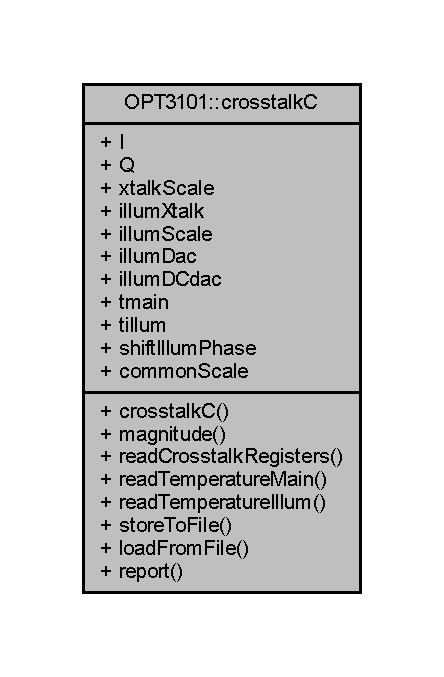
\includegraphics[width=213pt]{class_o_p_t3101_1_1crosstalk_c__coll__graph}
\end{center}
\end{figure}
\subsection*{Public Member Functions}
\begin{DoxyCompactItemize}
\item 
\mbox{\hyperlink{class_o_p_t3101_1_1crosstalk_c_a2b568d4391bfb9a92bbe74e88140bec0}{crosstalkC}} ()
\begin{DoxyCompactList}\small\item\em Constructor for class \mbox{\hyperlink{class_o_p_t3101_1_1crosstalk_c}{O\+P\+T3101\+::crosstalkC}} Constructor initializes the \mbox{\hyperlink{class_o_p_t3101_1_1crosstalk_c_a74d3bfbfb7da65511d2d16e1b66a7098}{O\+P\+T3101\+::crosstalk\+C\+::illum\+Xtalk}} parameter to a default false. \end{DoxyCompactList}\item 
double \mbox{\hyperlink{class_o_p_t3101_1_1crosstalk_c_a3f569027c07fb3fb49a02ae3108e34c1}{magnitude}} ()
\begin{DoxyCompactList}\small\item\em calculates magnitude This method calculates the magnitude of crosstalk represented in codes. Typical and good values for internal crosstalk is around 30. Typical and good values for illum crosstalk for highest current (170mA) $<$ 300 codes. \end{DoxyCompactList}\item 
void \mbox{\hyperlink{class_o_p_t3101_1_1crosstalk_c_acdfb870a70a6bc565d3a190fa459eeab}{read\+Crosstalk\+Registers}} (\mbox{\hyperlink{class_o_p_t3101_1_1device}{device}} $\ast$dev)
\begin{DoxyCompactList}\small\item\em reads the device 24 bit crosstalk registers This method reads the 24 bit crosstalk registers \mbox{\hyperlink{class_o_p_t3101_1_1registers_ae87864da6c35bed7c34ebf5f26ba4513}{O\+P\+T3101\+::registers\+::iphase\+\_\+xtalk}} and \mbox{\hyperlink{class_o_p_t3101_1_1registers_ad94d98dfb26313a9d32c5c2c0c673693}{O\+P\+T3101\+::registers\+::qphase\+\_\+xtalk}}. Translates them to 16 bit values and captures to \mbox{\hyperlink{class_o_p_t3101_1_1crosstalk_c_a97152b209288a0dc30c4158fdc1815fc}{O\+P\+T3101\+::crosstalk\+C\+::I}} \mbox{\hyperlink{class_o_p_t3101_1_1crosstalk_c_a1e20d913baf2432ec90fe06a45c226db}{O\+P\+T3101\+::crosstalk\+C\+::Q}} and \mbox{\hyperlink{class_o_p_t3101_1_1crosstalk_c_a5a5c560e1f5db427c02863a9618d9fa4}{O\+P\+T3101\+::crosstalk\+C\+::xtalk\+Scale}} \end{DoxyCompactList}\item 
void \mbox{\hyperlink{class_o_p_t3101_1_1crosstalk_c_a44bdf91acac0c969a89507ab2139e3b6}{read\+Temperature\+Main}} (\mbox{\hyperlink{class_o_p_t3101_1_1device}{device}} $\ast$dev)
\begin{DoxyCompactList}\small\item\em reads the temperature reading from main temp sensor This method reads the main temp sensor register O\+P\+T3101\+Register\+::tmain and captures to \mbox{\hyperlink{class_o_p_t3101_1_1crosstalk_c_a8b7250b531e953587c665c2c43860d82}{O\+P\+T3101\+::crosstalk\+C\+::tmain}} \end{DoxyCompactList}\item 
void \mbox{\hyperlink{class_o_p_t3101_1_1crosstalk_c_ad9045229556d3fe0c840e0e1113333d4}{read\+Temperature\+Illum}} (\mbox{\hyperlink{class_o_p_t3101_1_1device}{device}} $\ast$dev)
\begin{DoxyCompactList}\small\item\em reads the temperature reading from external temp sensor This method reads the main temp sensor register O\+P\+T3101\+Register\+::tillum and captures to \mbox{\hyperlink{class_o_p_t3101_1_1crosstalk_c_ab1d1d581f0495f5695ad49a2a8a41fd3}{O\+P\+T3101\+::crosstalk\+C\+::tillum}} \end{DoxyCompactList}\item 
void \mbox{\hyperlink{class_o_p_t3101_1_1crosstalk_c_a7d887d736dd5a3aa9dd81224e67240b8}{store\+To\+File}} (char $\ast$file\+Name)
\begin{DoxyCompactList}\small\item\em store crosstalk values to file This methods stores the crosstalk values to a non-\/volatile memory. Storage to non-\/volatile memory is important to be able to calculate temperature coefficient \mbox{\hyperlink{class_o_p_t3101_1_1crosstalk_temp_coff_c}{O\+P\+T3101\+::crosstalk\+Temp\+CoffC}} \end{DoxyCompactList}\item 
void \mbox{\hyperlink{class_o_p_t3101_1_1crosstalk_c_a8927a7e31870bf41a64d8b1755c6b0b2}{load\+From\+File}} (char $\ast$file\+Name)
\begin{DoxyCompactList}\small\item\em load crosstalk values from file This methods loads the crosstalk values to a non-\/volatile memory. Storage/\+Restoration to/from non-\/volatile memory is important to be able to calculate temperature coefficient \mbox{\hyperlink{class_o_p_t3101_1_1crosstalk_temp_coff_c}{O\+P\+T3101\+::crosstalk\+Temp\+CoffC}} \end{DoxyCompactList}\item 
void \mbox{\hyperlink{class_o_p_t3101_1_1crosstalk_c_a8a611602b13d6f3e97049696ddebe209}{report}} ()
\begin{DoxyCompactList}\small\item\em reports members of the instance Print the members of the class instance on screen \end{DoxyCompactList}\end{DoxyCompactItemize}
\subsection*{Public Attributes}
\begin{DoxyCompactItemize}
\item 
int16\+\_\+t \mbox{\hyperlink{class_o_p_t3101_1_1crosstalk_c_a97152b209288a0dc30c4158fdc1815fc}{I}}
\begin{DoxyCompactList}\small\item\em 16bit register setting for In phase component of the crosstalk \end{DoxyCompactList}\item 
int16\+\_\+t \mbox{\hyperlink{class_o_p_t3101_1_1crosstalk_c_a1e20d913baf2432ec90fe06a45c226db}{Q}}
\begin{DoxyCompactList}\small\item\em 16bit register setting for Quadrature phase component of the crosstalk \end{DoxyCompactList}\item 
uint8\+\_\+t \mbox{\hyperlink{class_o_p_t3101_1_1crosstalk_c_a5a5c560e1f5db427c02863a9618d9fa4}{xtalk\+Scale}}
\begin{DoxyCompactList}\small\item\em Crosstalk registers in \mbox{\hyperlink{namespace_o_p_t3101}{O\+P\+T3101}} device are 24 bit where as compensation registers are 16 bit. The scale parameter captures the scaling of the 24bit register to fit in to 16 bits. \end{DoxyCompactList}\item 
bool \mbox{\hyperlink{class_o_p_t3101_1_1crosstalk_c_a74d3bfbfb7da65511d2d16e1b66a7098}{illum\+Xtalk}}
\begin{DoxyCompactList}\small\item\em flag to capture if the crosstalk values belong to internal crosstalk (false) or illum crosstalk (true) \end{DoxyCompactList}\item 
uint8\+\_\+t \mbox{\hyperlink{class_o_p_t3101_1_1crosstalk_c_aa9790b90a4d30f9459ef30c2ffcb0f15}{illum\+Scale}}
\begin{DoxyCompactList}\small\item\em Member that captures the snapshot of illumination current multiplier scale register during crosstalk measurement for analysis. \end{DoxyCompactList}\item 
uint8\+\_\+t \mbox{\hyperlink{class_o_p_t3101_1_1crosstalk_c_a926366d3812a768269de408d4205bdec}{illum\+Dac}}
\begin{DoxyCompactList}\small\item\em Member that captures the snapshot of illumination current setting register during crosstalk measurement for analysis. \end{DoxyCompactList}\item 
uint8\+\_\+t \mbox{\hyperlink{class_o_p_t3101_1_1crosstalk_c_aa25494ff4a32e26e0abfa158b2e60808}{illum\+D\+Cdac}}
\begin{DoxyCompactList}\small\item\em Member that captures the snapshot of illumination DC current setting register during crosstalk measurement for analysis. \end{DoxyCompactList}\item 
uint16\+\_\+t \mbox{\hyperlink{class_o_p_t3101_1_1crosstalk_c_a8b7250b531e953587c665c2c43860d82}{tmain}}
\begin{DoxyCompactList}\small\item\em Member that captures the snapshot of temperature of main temp sensor during crosstalk measurement. \end{DoxyCompactList}\item 
uint16\+\_\+t \mbox{\hyperlink{class_o_p_t3101_1_1crosstalk_c_ab1d1d581f0495f5695ad49a2a8a41fd3}{tillum}}
\begin{DoxyCompactList}\small\item\em Member that captures the snapshot of temperature of external temp sensor during crosstalk measurement. \end{DoxyCompactList}\item 
uint8\+\_\+t \mbox{\hyperlink{class_o_p_t3101_1_1crosstalk_c_ae60d9239aa603895c534e954ee87c613}{shift\+Illum\+Phase}}
\begin{DoxyCompactList}\small\item\em Member that captures the snapshot of shift illum phase during crosstalk measurement. \end{DoxyCompactList}\item 
uint8\+\_\+t \mbox{\hyperlink{class_o_p_t3101_1_1crosstalk_c_a933c7f37d5a48d74a4dd783cf07ed040}{common\+Scale}}
\begin{DoxyCompactList}\small\item\em Member that captures the common scale to be applied to all the crosstalk values to be applied \mbox{\hyperlink{namespace_o_p_t3101}{O\+P\+T3101}} device during facotry \mbox{\hyperlink{class_o_p_t3101_1_1calibration_c}{calibrationC}}. This value is calculated as a common value based on a bunch of \mbox{\hyperlink{class_o_p_t3101_1_1crosstalk_c}{O\+P\+T3101\+::crosstalkC}} instances. \end{DoxyCompactList}\end{DoxyCompactItemize}
\subsection*{Friends}
\begin{DoxyCompactItemize}
\item 
std\+::ostream \& \mbox{\hyperlink{class_o_p_t3101_1_1crosstalk_c_a759466b2ca88c3105614f17a571e4d08}{operator$<$$<$}} (std\+::ostream \&os, const \mbox{\hyperlink{class_o_p_t3101_1_1crosstalk_c}{crosstalkC}} $\ast$data)
\begin{DoxyCompactList}\small\item\em Operator overload to store class contents to a file Casts all the class members for file storage. \end{DoxyCompactList}\item 
std\+::istream \& \mbox{\hyperlink{class_o_p_t3101_1_1crosstalk_c_a71fdefefe0fa23c7baaa915320867f7d}{operator$>$$>$}} (std\+::istream \&is, \mbox{\hyperlink{class_o_p_t3101_1_1crosstalk_c}{crosstalkC}} $\ast$data)
\begin{DoxyCompactList}\small\item\em Operator overload to load class contents to from a file Retreives all the class members from a stored file. \end{DoxyCompactList}\end{DoxyCompactItemize}


\subsection{Detailed Description}
Class that holds crosstalk related registers and values. 

This is a class container that can hold crosstalk values. \mbox{\hyperlink{namespace_o_p_t3101}{O\+P\+T3101}} device has different crosstalk phenomenon which needs to be calibrated and compensated~\newline
 There are primarily 2 types of crosstalk phenomenon that need to be compensated or calibrated out to achieve good system performance. ~\newline

\begin{DoxyEnumerate}
\item Internal crosstalk
\begin{DoxyEnumerate}
\item This is defined as the amount of signal measured by A\+FE when there the TX channels are turned O\+FF. Internal crosstalk phenomenon occurs due to coupling from power supply and ground.~\newline

\item This phenomenon is independent of TX channel or configuration since the TX channels are off.
\end{DoxyEnumerate}
\item Illum crosstalk
\begin{DoxyEnumerate}
\item This is defined as the amount of signal measured by A\+FE when the TX channels are turned ON and the system is pointing to infinity or with photo diode covered.
\item This phenomenon is highly dependent on TX channel and the current settings on each TX.
\end{DoxyEnumerate}
\end{DoxyEnumerate}

\mbox{\hyperlink{namespace_o_p_t3101}{O\+P\+T3101}} device has internal registers to correct and compensate for different crosstalk phenomenon. This class acts as a temporary storage of crosstalk values measured. Calculations have to be made on the crosstalk values to transform them to register settings. Besides that other \mbox{\hyperlink{class_o_p_t3101_1_1calibration_c}{calibrationC}} coefficients like \mbox{\hyperlink{class_o_p_t3101_1_1crosstalk_temp_coff_c}{O\+P\+T3101\+::crosstalk\+Temp\+CoffC}} will be calculated. 

\subsection{Constructor \& Destructor Documentation}
\mbox{\Hypertarget{class_o_p_t3101_1_1crosstalk_c_a2b568d4391bfb9a92bbe74e88140bec0}\label{class_o_p_t3101_1_1crosstalk_c_a2b568d4391bfb9a92bbe74e88140bec0}} 
\index{O\+P\+T3101\+::crosstalkC@{O\+P\+T3101\+::crosstalkC}!crosstalkC@{crosstalkC}}
\index{crosstalkC@{crosstalkC}!O\+P\+T3101\+::crosstalkC@{O\+P\+T3101\+::crosstalkC}}
\subsubsection{\texorpdfstring{crosstalk\+C()}{crosstalkC()}}
{\footnotesize\ttfamily O\+P\+T3101\+::crosstalk\+C\+::crosstalkC (\begin{DoxyParamCaption}{ }\end{DoxyParamCaption})}



Constructor for class \mbox{\hyperlink{class_o_p_t3101_1_1crosstalk_c}{O\+P\+T3101\+::crosstalkC}} Constructor initializes the \mbox{\hyperlink{class_o_p_t3101_1_1crosstalk_c_a74d3bfbfb7da65511d2d16e1b66a7098}{O\+P\+T3101\+::crosstalk\+C\+::illum\+Xtalk}} parameter to a default false. 

{\bfseries Algorithm of the method is as follows}


\begin{DoxyItemize}
\item sets \mbox{\hyperlink{class_o_p_t3101_1_1crosstalk_c_a74d3bfbfb7da65511d2d16e1b66a7098}{O\+P\+T3101\+::crosstalk\+C\+::illum\+Xtalk}} to false by default 
\end{DoxyItemize}

\subsection{Member Function Documentation}
\mbox{\Hypertarget{class_o_p_t3101_1_1crosstalk_c_a8927a7e31870bf41a64d8b1755c6b0b2}\label{class_o_p_t3101_1_1crosstalk_c_a8927a7e31870bf41a64d8b1755c6b0b2}} 
\index{O\+P\+T3101\+::crosstalkC@{O\+P\+T3101\+::crosstalkC}!load\+From\+File@{load\+From\+File}}
\index{load\+From\+File@{load\+From\+File}!O\+P\+T3101\+::crosstalkC@{O\+P\+T3101\+::crosstalkC}}
\subsubsection{\texorpdfstring{load\+From\+File()}{loadFromFile()}}
{\footnotesize\ttfamily void O\+P\+T3101\+::crosstalk\+C\+::load\+From\+File (\begin{DoxyParamCaption}\item[{char $\ast$}]{file\+Name }\end{DoxyParamCaption})}



load crosstalk values from file This methods loads the crosstalk values to a non-\/volatile memory. Storage/\+Restoration to/from non-\/volatile memory is important to be able to calculate temperature coefficient \mbox{\hyperlink{class_o_p_t3101_1_1crosstalk_temp_coff_c}{O\+P\+T3101\+::crosstalk\+Temp\+CoffC}} 


\begin{DoxyParams}[1]{Parameters}
\mbox{\tt in}  & {\em file\+Name;} & Path and name of the file from where the crosstalk values are loaded \\
\hline
\end{DoxyParams}
\begin{DoxyReturn}{Returns}
Nothing; 
\end{DoxyReturn}
{\bfseries Algorithm of the method is as follows}


\begin{DoxyItemize}
\item User needs to implement file load/restore based on host. 
\end{DoxyItemize}\mbox{\Hypertarget{class_o_p_t3101_1_1crosstalk_c_a3f569027c07fb3fb49a02ae3108e34c1}\label{class_o_p_t3101_1_1crosstalk_c_a3f569027c07fb3fb49a02ae3108e34c1}} 
\index{O\+P\+T3101\+::crosstalkC@{O\+P\+T3101\+::crosstalkC}!magnitude@{magnitude}}
\index{magnitude@{magnitude}!O\+P\+T3101\+::crosstalkC@{O\+P\+T3101\+::crosstalkC}}
\subsubsection{\texorpdfstring{magnitude()}{magnitude()}}
{\footnotesize\ttfamily double O\+P\+T3101\+::crosstalk\+C\+::magnitude (\begin{DoxyParamCaption}{ }\end{DoxyParamCaption})}



calculates magnitude This method calculates the magnitude of crosstalk represented in codes. Typical and good values for internal crosstalk is around 30. Typical and good values for illum crosstalk for highest current (170mA) $<$ 300 codes. 

\begin{DoxyReturn}{Returns}
magnitude of crosstalk; 
\end{DoxyReturn}
{\bfseries Algorithm of the method is as follows}


\begin{DoxyItemize}
\item Calculates the magnitude of crosstalk based on a predefined formula. {\bfseries Warning\+:} This uses floating point arithmetic and math.\+h library for power and sqrt functions 
\end{DoxyItemize}\mbox{\Hypertarget{class_o_p_t3101_1_1crosstalk_c_acdfb870a70a6bc565d3a190fa459eeab}\label{class_o_p_t3101_1_1crosstalk_c_acdfb870a70a6bc565d3a190fa459eeab}} 
\index{O\+P\+T3101\+::crosstalkC@{O\+P\+T3101\+::crosstalkC}!read\+Crosstalk\+Registers@{read\+Crosstalk\+Registers}}
\index{read\+Crosstalk\+Registers@{read\+Crosstalk\+Registers}!O\+P\+T3101\+::crosstalkC@{O\+P\+T3101\+::crosstalkC}}
\subsubsection{\texorpdfstring{read\+Crosstalk\+Registers()}{readCrosstalkRegisters()}}
{\footnotesize\ttfamily void O\+P\+T3101\+::crosstalk\+C\+::read\+Crosstalk\+Registers (\begin{DoxyParamCaption}\item[{\mbox{\hyperlink{class_o_p_t3101_1_1device}{O\+P\+T3101\+::device}} $\ast$}]{dev }\end{DoxyParamCaption})}



reads the device 24 bit crosstalk registers This method reads the 24 bit crosstalk registers \mbox{\hyperlink{class_o_p_t3101_1_1registers_ae87864da6c35bed7c34ebf5f26ba4513}{O\+P\+T3101\+::registers\+::iphase\+\_\+xtalk}} and \mbox{\hyperlink{class_o_p_t3101_1_1registers_ad94d98dfb26313a9d32c5c2c0c673693}{O\+P\+T3101\+::registers\+::qphase\+\_\+xtalk}}. Translates them to 16 bit values and captures to \mbox{\hyperlink{class_o_p_t3101_1_1crosstalk_c_a97152b209288a0dc30c4158fdc1815fc}{O\+P\+T3101\+::crosstalk\+C\+::I}} \mbox{\hyperlink{class_o_p_t3101_1_1crosstalk_c_a1e20d913baf2432ec90fe06a45c226db}{O\+P\+T3101\+::crosstalk\+C\+::Q}} and \mbox{\hyperlink{class_o_p_t3101_1_1crosstalk_c_a5a5c560e1f5db427c02863a9618d9fa4}{O\+P\+T3101\+::crosstalk\+C\+::xtalk\+Scale}} 


\begin{DoxyParams}[1]{Parameters}
\mbox{\tt in}  & {\em dev;} & The dev is pointer to class \mbox{\hyperlink{class_o_p_t3101_1_1device}{O\+P\+T3101\+::device}} . This is required to realize I2C transactions and register map \\
\hline
\end{DoxyParams}
\begin{DoxyReturn}{Returns}
Nothing; 
\end{DoxyReturn}
{\bfseries Algorithm of the method is as follows}


\begin{DoxyItemize}
\item Reads register \mbox{\hyperlink{class_o_p_t3101_1_1registers_ae87864da6c35bed7c34ebf5f26ba4513}{O\+P\+T3101\+::registers\+::iphase\+\_\+xtalk}} in 24 bit from and converts to signed number
\item Reads register \mbox{\hyperlink{class_o_p_t3101_1_1registers_ad94d98dfb26313a9d32c5c2c0c673693}{O\+P\+T3101\+::registers\+::qphase\+\_\+xtalk}} in 24 bit from and converts to signed number
\item Finds absolute max among the read I and Q register values to determine the \mbox{\hyperlink{class_o_p_t3101_1_1crosstalk_c_a74d3bfbfb7da65511d2d16e1b66a7098}{O\+P\+T3101\+::crosstalk\+C\+::illum\+Xtalk}}
\item Determines \mbox{\hyperlink{class_o_p_t3101_1_1crosstalk_c_a74d3bfbfb7da65511d2d16e1b66a7098}{O\+P\+T3101\+::crosstalk\+C\+::illum\+Xtalk}} and assigns. The algorithm finds the minimum \mbox{\hyperlink{class_o_p_t3101_1_1crosstalk_c_a74d3bfbfb7da65511d2d16e1b66a7098}{O\+P\+T3101\+::crosstalk\+C\+::illum\+Xtalk}} value for which the raw I and Q registers can be fit to a 16 bit register ~\newline

\item Scales down the 24 bit raw register I and Q values with \mbox{\hyperlink{class_o_p_t3101_1_1crosstalk_c_a74d3bfbfb7da65511d2d16e1b66a7098}{O\+P\+T3101\+::crosstalk\+C\+::illum\+Xtalk}} and assigns to \mbox{\hyperlink{class_o_p_t3101_1_1crosstalk_c_a97152b209288a0dc30c4158fdc1815fc}{O\+P\+T3101\+::crosstalk\+C\+::I}} and \mbox{\hyperlink{class_o_p_t3101_1_1crosstalk_c_a1e20d913baf2432ec90fe06a45c226db}{O\+P\+T3101\+::crosstalk\+C\+::Q}} 
\end{DoxyItemize}\mbox{\Hypertarget{class_o_p_t3101_1_1crosstalk_c_ad9045229556d3fe0c840e0e1113333d4}\label{class_o_p_t3101_1_1crosstalk_c_ad9045229556d3fe0c840e0e1113333d4}} 
\index{O\+P\+T3101\+::crosstalkC@{O\+P\+T3101\+::crosstalkC}!read\+Temperature\+Illum@{read\+Temperature\+Illum}}
\index{read\+Temperature\+Illum@{read\+Temperature\+Illum}!O\+P\+T3101\+::crosstalkC@{O\+P\+T3101\+::crosstalkC}}
\subsubsection{\texorpdfstring{read\+Temperature\+Illum()}{readTemperatureIllum()}}
{\footnotesize\ttfamily void O\+P\+T3101\+::crosstalk\+C\+::read\+Temperature\+Illum (\begin{DoxyParamCaption}\item[{\mbox{\hyperlink{class_o_p_t3101_1_1device}{O\+P\+T3101\+::device}} $\ast$}]{dev }\end{DoxyParamCaption})}



reads the temperature reading from external temp sensor This method reads the main temp sensor register O\+P\+T3101\+Register\+::tillum and captures to \mbox{\hyperlink{class_o_p_t3101_1_1crosstalk_c_ab1d1d581f0495f5695ad49a2a8a41fd3}{O\+P\+T3101\+::crosstalk\+C\+::tillum}} 


\begin{DoxyParams}[1]{Parameters}
\mbox{\tt in}  & {\em dev;} & The dev is pointer to class \mbox{\hyperlink{class_o_p_t3101_1_1device}{O\+P\+T3101\+::device}} . This is required to realize I2C transactions and register map \\
\hline
\end{DoxyParams}
\begin{DoxyReturn}{Returns}
Nothing; 
\end{DoxyReturn}
{\bfseries Algorithm of the method is as follows}


\begin{DoxyItemize}
\item Reads register O\+P\+T3101\+Register\+::illum and assigns to O\+P\+T3101\+::crosstalk\+C\+::illum 
\end{DoxyItemize}\mbox{\Hypertarget{class_o_p_t3101_1_1crosstalk_c_a44bdf91acac0c969a89507ab2139e3b6}\label{class_o_p_t3101_1_1crosstalk_c_a44bdf91acac0c969a89507ab2139e3b6}} 
\index{O\+P\+T3101\+::crosstalkC@{O\+P\+T3101\+::crosstalkC}!read\+Temperature\+Main@{read\+Temperature\+Main}}
\index{read\+Temperature\+Main@{read\+Temperature\+Main}!O\+P\+T3101\+::crosstalkC@{O\+P\+T3101\+::crosstalkC}}
\subsubsection{\texorpdfstring{read\+Temperature\+Main()}{readTemperatureMain()}}
{\footnotesize\ttfamily void O\+P\+T3101\+::crosstalk\+C\+::read\+Temperature\+Main (\begin{DoxyParamCaption}\item[{\mbox{\hyperlink{class_o_p_t3101_1_1device}{O\+P\+T3101\+::device}} $\ast$}]{dev }\end{DoxyParamCaption})}



reads the temperature reading from main temp sensor This method reads the main temp sensor register O\+P\+T3101\+Register\+::tmain and captures to \mbox{\hyperlink{class_o_p_t3101_1_1crosstalk_c_a8b7250b531e953587c665c2c43860d82}{O\+P\+T3101\+::crosstalk\+C\+::tmain}} 


\begin{DoxyParams}[1]{Parameters}
\mbox{\tt in}  & {\em dev;} & The dev is pointer to class \mbox{\hyperlink{class_o_p_t3101_1_1device}{O\+P\+T3101\+::device}} . This is required to realize I2C transactions and register map \\
\hline
\end{DoxyParams}
\begin{DoxyReturn}{Returns}
Nothing; 
\end{DoxyReturn}
{\bfseries Algorithm of the method is as follows}


\begin{DoxyItemize}
\item Reads register O\+P\+T3101\+Register\+::tmain and assigns to \mbox{\hyperlink{class_o_p_t3101_1_1crosstalk_c_a8b7250b531e953587c665c2c43860d82}{O\+P\+T3101\+::crosstalk\+C\+::tmain}} 
\end{DoxyItemize}\mbox{\Hypertarget{class_o_p_t3101_1_1crosstalk_c_a8a611602b13d6f3e97049696ddebe209}\label{class_o_p_t3101_1_1crosstalk_c_a8a611602b13d6f3e97049696ddebe209}} 
\index{O\+P\+T3101\+::crosstalkC@{O\+P\+T3101\+::crosstalkC}!report@{report}}
\index{report@{report}!O\+P\+T3101\+::crosstalkC@{O\+P\+T3101\+::crosstalkC}}
\subsubsection{\texorpdfstring{report()}{report()}}
{\footnotesize\ttfamily void O\+P\+T3101\+::crosstalk\+C\+::report (\begin{DoxyParamCaption}{ }\end{DoxyParamCaption})}



reports members of the instance Print the members of the class instance on screen 

\begin{DoxyReturn}{Returns}
Nothing; 
\end{DoxyReturn}
{\bfseries Algorithm of the method is as follows}


\begin{DoxyItemize}
\item Prints all the members and values of members on screen. ~\newline

\item User needs to implement file load/restore based on host. 
\end{DoxyItemize}\mbox{\Hypertarget{class_o_p_t3101_1_1crosstalk_c_a7d887d736dd5a3aa9dd81224e67240b8}\label{class_o_p_t3101_1_1crosstalk_c_a7d887d736dd5a3aa9dd81224e67240b8}} 
\index{O\+P\+T3101\+::crosstalkC@{O\+P\+T3101\+::crosstalkC}!store\+To\+File@{store\+To\+File}}
\index{store\+To\+File@{store\+To\+File}!O\+P\+T3101\+::crosstalkC@{O\+P\+T3101\+::crosstalkC}}
\subsubsection{\texorpdfstring{store\+To\+File()}{storeToFile()}}
{\footnotesize\ttfamily void O\+P\+T3101\+::crosstalk\+C\+::store\+To\+File (\begin{DoxyParamCaption}\item[{char $\ast$}]{file\+Name }\end{DoxyParamCaption})}



store crosstalk values to file This methods stores the crosstalk values to a non-\/volatile memory. Storage to non-\/volatile memory is important to be able to calculate temperature coefficient \mbox{\hyperlink{class_o_p_t3101_1_1crosstalk_temp_coff_c}{O\+P\+T3101\+::crosstalk\+Temp\+CoffC}} 


\begin{DoxyParams}[1]{Parameters}
\mbox{\tt in}  & {\em file\+Name;} & Path and name of the file to capture the crosstalk values to \\
\hline
\end{DoxyParams}
\begin{DoxyReturn}{Returns}
Nothing; 
\end{DoxyReturn}
{\bfseries Algorithm of the method is as follows}


\begin{DoxyItemize}
\item User needs to implement file storage based on host. 
\end{DoxyItemize}

\subsection{Friends And Related Function Documentation}
\mbox{\Hypertarget{class_o_p_t3101_1_1crosstalk_c_a759466b2ca88c3105614f17a571e4d08}\label{class_o_p_t3101_1_1crosstalk_c_a759466b2ca88c3105614f17a571e4d08}} 
\index{O\+P\+T3101\+::crosstalkC@{O\+P\+T3101\+::crosstalkC}!operator$<$$<$@{operator$<$$<$}}
\index{operator$<$$<$@{operator$<$$<$}!O\+P\+T3101\+::crosstalkC@{O\+P\+T3101\+::crosstalkC}}
\subsubsection{\texorpdfstring{operator$<$$<$}{operator<<}}
{\footnotesize\ttfamily std\+::ostream\& operator$<$$<$ (\begin{DoxyParamCaption}\item[{std\+::ostream \&}]{os,  }\item[{const \mbox{\hyperlink{class_o_p_t3101_1_1crosstalk_c}{crosstalkC}} $\ast$}]{data }\end{DoxyParamCaption})\hspace{0.3cm}{\ttfamily [friend]}}



Operator overload to store class contents to a file Casts all the class members for file storage. 


\begin{DoxyParams}[1]{Parameters}
\mbox{\tt out}  & {\em os;} & os is data stream to serialize data \\
\hline
\mbox{\tt in}  & {\em data;} & data is pointer to the class to be serialzied and stored \\
\hline
\end{DoxyParams}
\begin{DoxyReturn}{Returns}
std\+::ostream; Serialized std\+::ostream to be written to a file 
\end{DoxyReturn}
\mbox{\Hypertarget{class_o_p_t3101_1_1crosstalk_c_a71fdefefe0fa23c7baaa915320867f7d}\label{class_o_p_t3101_1_1crosstalk_c_a71fdefefe0fa23c7baaa915320867f7d}} 
\index{O\+P\+T3101\+::crosstalkC@{O\+P\+T3101\+::crosstalkC}!operator$>$$>$@{operator$>$$>$}}
\index{operator$>$$>$@{operator$>$$>$}!O\+P\+T3101\+::crosstalkC@{O\+P\+T3101\+::crosstalkC}}
\subsubsection{\texorpdfstring{operator$>$$>$}{operator>>}}
{\footnotesize\ttfamily std\+::istream\& operator$>$$>$ (\begin{DoxyParamCaption}\item[{std\+::istream \&}]{is,  }\item[{\mbox{\hyperlink{class_o_p_t3101_1_1crosstalk_c}{crosstalkC}} $\ast$}]{data }\end{DoxyParamCaption})\hspace{0.3cm}{\ttfamily [friend]}}



Operator overload to load class contents to from a file Retreives all the class members from a stored file. 


\begin{DoxyParams}[1]{Parameters}
\mbox{\tt in}  & {\em is;} & is input stream from where the data is loaded \\
\hline
\mbox{\tt out}  & {\em data;} & data is pointer to the class to be restored \\
\hline
\end{DoxyParams}
\begin{DoxyReturn}{Returns}
std\+::istream; Serialized Input stream loaded from file 
\end{DoxyReturn}


\subsection{Member Data Documentation}
\mbox{\Hypertarget{class_o_p_t3101_1_1crosstalk_c_a933c7f37d5a48d74a4dd783cf07ed040}\label{class_o_p_t3101_1_1crosstalk_c_a933c7f37d5a48d74a4dd783cf07ed040}} 
\index{O\+P\+T3101\+::crosstalkC@{O\+P\+T3101\+::crosstalkC}!common\+Scale@{common\+Scale}}
\index{common\+Scale@{common\+Scale}!O\+P\+T3101\+::crosstalkC@{O\+P\+T3101\+::crosstalkC}}
\subsubsection{\texorpdfstring{common\+Scale}{commonScale}}
{\footnotesize\ttfamily uint8\+\_\+t O\+P\+T3101\+::crosstalk\+C\+::common\+Scale}



Member that captures the common scale to be applied to all the crosstalk values to be applied \mbox{\hyperlink{namespace_o_p_t3101}{O\+P\+T3101}} device during facotry \mbox{\hyperlink{class_o_p_t3101_1_1calibration_c}{calibrationC}}. This value is calculated as a common value based on a bunch of \mbox{\hyperlink{class_o_p_t3101_1_1crosstalk_c}{O\+P\+T3101\+::crosstalkC}} instances. 

\mbox{\Hypertarget{class_o_p_t3101_1_1crosstalk_c_a97152b209288a0dc30c4158fdc1815fc}\label{class_o_p_t3101_1_1crosstalk_c_a97152b209288a0dc30c4158fdc1815fc}} 
\index{O\+P\+T3101\+::crosstalkC@{O\+P\+T3101\+::crosstalkC}!I@{I}}
\index{I@{I}!O\+P\+T3101\+::crosstalkC@{O\+P\+T3101\+::crosstalkC}}
\subsubsection{\texorpdfstring{I}{I}}
{\footnotesize\ttfamily int16\+\_\+t O\+P\+T3101\+::crosstalk\+C\+::I}



16bit register setting for In phase component of the crosstalk 

\mbox{\Hypertarget{class_o_p_t3101_1_1crosstalk_c_a926366d3812a768269de408d4205bdec}\label{class_o_p_t3101_1_1crosstalk_c_a926366d3812a768269de408d4205bdec}} 
\index{O\+P\+T3101\+::crosstalkC@{O\+P\+T3101\+::crosstalkC}!illum\+Dac@{illum\+Dac}}
\index{illum\+Dac@{illum\+Dac}!O\+P\+T3101\+::crosstalkC@{O\+P\+T3101\+::crosstalkC}}
\subsubsection{\texorpdfstring{illum\+Dac}{illumDac}}
{\footnotesize\ttfamily uint8\+\_\+t O\+P\+T3101\+::crosstalk\+C\+::illum\+Dac}



Member that captures the snapshot of illumination current setting register during crosstalk measurement for analysis. 

\mbox{\Hypertarget{class_o_p_t3101_1_1crosstalk_c_aa25494ff4a32e26e0abfa158b2e60808}\label{class_o_p_t3101_1_1crosstalk_c_aa25494ff4a32e26e0abfa158b2e60808}} 
\index{O\+P\+T3101\+::crosstalkC@{O\+P\+T3101\+::crosstalkC}!illum\+D\+Cdac@{illum\+D\+Cdac}}
\index{illum\+D\+Cdac@{illum\+D\+Cdac}!O\+P\+T3101\+::crosstalkC@{O\+P\+T3101\+::crosstalkC}}
\subsubsection{\texorpdfstring{illum\+D\+Cdac}{illumDCdac}}
{\footnotesize\ttfamily uint8\+\_\+t O\+P\+T3101\+::crosstalk\+C\+::illum\+D\+Cdac}



Member that captures the snapshot of illumination DC current setting register during crosstalk measurement for analysis. 

\mbox{\Hypertarget{class_o_p_t3101_1_1crosstalk_c_aa9790b90a4d30f9459ef30c2ffcb0f15}\label{class_o_p_t3101_1_1crosstalk_c_aa9790b90a4d30f9459ef30c2ffcb0f15}} 
\index{O\+P\+T3101\+::crosstalkC@{O\+P\+T3101\+::crosstalkC}!illum\+Scale@{illum\+Scale}}
\index{illum\+Scale@{illum\+Scale}!O\+P\+T3101\+::crosstalkC@{O\+P\+T3101\+::crosstalkC}}
\subsubsection{\texorpdfstring{illum\+Scale}{illumScale}}
{\footnotesize\ttfamily uint8\+\_\+t O\+P\+T3101\+::crosstalk\+C\+::illum\+Scale}



Member that captures the snapshot of illumination current multiplier scale register during crosstalk measurement for analysis. 

\mbox{\Hypertarget{class_o_p_t3101_1_1crosstalk_c_a74d3bfbfb7da65511d2d16e1b66a7098}\label{class_o_p_t3101_1_1crosstalk_c_a74d3bfbfb7da65511d2d16e1b66a7098}} 
\index{O\+P\+T3101\+::crosstalkC@{O\+P\+T3101\+::crosstalkC}!illum\+Xtalk@{illum\+Xtalk}}
\index{illum\+Xtalk@{illum\+Xtalk}!O\+P\+T3101\+::crosstalkC@{O\+P\+T3101\+::crosstalkC}}
\subsubsection{\texorpdfstring{illum\+Xtalk}{illumXtalk}}
{\footnotesize\ttfamily bool O\+P\+T3101\+::crosstalk\+C\+::illum\+Xtalk}



flag to capture if the crosstalk values belong to internal crosstalk (false) or illum crosstalk (true) 

\mbox{\Hypertarget{class_o_p_t3101_1_1crosstalk_c_a1e20d913baf2432ec90fe06a45c226db}\label{class_o_p_t3101_1_1crosstalk_c_a1e20d913baf2432ec90fe06a45c226db}} 
\index{O\+P\+T3101\+::crosstalkC@{O\+P\+T3101\+::crosstalkC}!Q@{Q}}
\index{Q@{Q}!O\+P\+T3101\+::crosstalkC@{O\+P\+T3101\+::crosstalkC}}
\subsubsection{\texorpdfstring{Q}{Q}}
{\footnotesize\ttfamily int16\+\_\+t O\+P\+T3101\+::crosstalk\+C\+::Q}



16bit register setting for Quadrature phase component of the crosstalk 

\mbox{\Hypertarget{class_o_p_t3101_1_1crosstalk_c_ae60d9239aa603895c534e954ee87c613}\label{class_o_p_t3101_1_1crosstalk_c_ae60d9239aa603895c534e954ee87c613}} 
\index{O\+P\+T3101\+::crosstalkC@{O\+P\+T3101\+::crosstalkC}!shift\+Illum\+Phase@{shift\+Illum\+Phase}}
\index{shift\+Illum\+Phase@{shift\+Illum\+Phase}!O\+P\+T3101\+::crosstalkC@{O\+P\+T3101\+::crosstalkC}}
\subsubsection{\texorpdfstring{shift\+Illum\+Phase}{shiftIllumPhase}}
{\footnotesize\ttfamily uint8\+\_\+t O\+P\+T3101\+::crosstalk\+C\+::shift\+Illum\+Phase}



Member that captures the snapshot of shift illum phase during crosstalk measurement. 

\mbox{\Hypertarget{class_o_p_t3101_1_1crosstalk_c_ab1d1d581f0495f5695ad49a2a8a41fd3}\label{class_o_p_t3101_1_1crosstalk_c_ab1d1d581f0495f5695ad49a2a8a41fd3}} 
\index{O\+P\+T3101\+::crosstalkC@{O\+P\+T3101\+::crosstalkC}!tillum@{tillum}}
\index{tillum@{tillum}!O\+P\+T3101\+::crosstalkC@{O\+P\+T3101\+::crosstalkC}}
\subsubsection{\texorpdfstring{tillum}{tillum}}
{\footnotesize\ttfamily uint16\+\_\+t O\+P\+T3101\+::crosstalk\+C\+::tillum}



Member that captures the snapshot of temperature of external temp sensor during crosstalk measurement. 

\mbox{\Hypertarget{class_o_p_t3101_1_1crosstalk_c_a8b7250b531e953587c665c2c43860d82}\label{class_o_p_t3101_1_1crosstalk_c_a8b7250b531e953587c665c2c43860d82}} 
\index{O\+P\+T3101\+::crosstalkC@{O\+P\+T3101\+::crosstalkC}!tmain@{tmain}}
\index{tmain@{tmain}!O\+P\+T3101\+::crosstalkC@{O\+P\+T3101\+::crosstalkC}}
\subsubsection{\texorpdfstring{tmain}{tmain}}
{\footnotesize\ttfamily uint16\+\_\+t O\+P\+T3101\+::crosstalk\+C\+::tmain}



Member that captures the snapshot of temperature of main temp sensor during crosstalk measurement. 

\mbox{\Hypertarget{class_o_p_t3101_1_1crosstalk_c_a5a5c560e1f5db427c02863a9618d9fa4}\label{class_o_p_t3101_1_1crosstalk_c_a5a5c560e1f5db427c02863a9618d9fa4}} 
\index{O\+P\+T3101\+::crosstalkC@{O\+P\+T3101\+::crosstalkC}!xtalk\+Scale@{xtalk\+Scale}}
\index{xtalk\+Scale@{xtalk\+Scale}!O\+P\+T3101\+::crosstalkC@{O\+P\+T3101\+::crosstalkC}}
\subsubsection{\texorpdfstring{xtalk\+Scale}{xtalkScale}}
{\footnotesize\ttfamily uint8\+\_\+t O\+P\+T3101\+::crosstalk\+C\+::xtalk\+Scale}



Crosstalk registers in \mbox{\hyperlink{namespace_o_p_t3101}{O\+P\+T3101}} device are 24 bit where as compensation registers are 16 bit. The scale parameter captures the scaling of the 24bit register to fit in to 16 bits. 



The documentation for this class was generated from the following files\+:\begin{DoxyCompactItemize}
\item 
C\+:/folders/d/scripts/cpp/\+O\+P\+T3101\+S\+D\+K/\+O\+P\+T3101\+S\+D\+K/\+O\+P\+T3101\+S\+D\+K/\mbox{\hyperlink{_o_p_t3101_crosstalk_8h}{O\+P\+T3101\+Crosstalk.\+h}}\item 
C\+:/folders/d/scripts/cpp/\+O\+P\+T3101\+S\+D\+K/\+O\+P\+T3101\+S\+D\+K/\+O\+P\+T3101\+S\+D\+K/\mbox{\hyperlink{_o_p_t3101_crosstalk_8cpp}{O\+P\+T3101\+Crosstalk.\+cpp}}\end{DoxyCompactItemize}

\hypertarget{class_o_p_t3101_1_1crosstalk_temp_coff_c}{}\section{O\+P\+T3101\+:\+:crosstalk\+Temp\+CoffC Class Reference}
\label{class_o_p_t3101_1_1crosstalk_temp_coff_c}\index{O\+P\+T3101\+::crosstalk\+Temp\+CoffC@{O\+P\+T3101\+::crosstalk\+Temp\+CoffC}}


Class that holds crosstalk temperature coefficient related registers and values.  




{\ttfamily \#include $<$O\+P\+T3101\+Design\+Coefficients.\+h$>$}



Collaboration diagram for O\+P\+T3101\+:\+:crosstalk\+Temp\+CoffC\+:\nopagebreak
\begin{figure}[H]
\begin{center}
\leavevmode
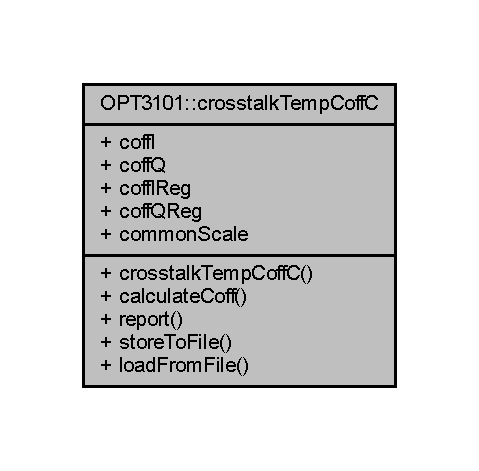
\includegraphics[width=230pt]{class_o_p_t3101_1_1crosstalk_temp_coff_c__coll__graph}
\end{center}
\end{figure}
\subsection*{Public Member Functions}
\begin{DoxyCompactItemize}
\item 
\mbox{\hyperlink{class_o_p_t3101_1_1crosstalk_temp_coff_c_a3e910a6053a8cbffb8d18868ade903b5}{crosstalk\+Temp\+CoffC}} ()
\begin{DoxyCompactList}\small\item\em initializes the members to 0 \end{DoxyCompactList}\item 
void \mbox{\hyperlink{class_o_p_t3101_1_1crosstalk_temp_coff_c_a21c8e56e8f2b313d3f89c6e989a8aee2}{calculate\+Coff}} (\mbox{\hyperlink{class_o_p_t3101_1_1crosstalk_c}{crosstalkC}} $\ast$illum\+Xtalk0, \mbox{\hyperlink{class_o_p_t3101_1_1crosstalk_c}{crosstalkC}} $\ast$illum\+Xtalk1)
\begin{DoxyCompactList}\small\item\em calculates the crosstalk temp coff \end{DoxyCompactList}\item 
void \mbox{\hyperlink{class_o_p_t3101_1_1crosstalk_temp_coff_c_a881ec5ebe971af6c4c4f50e143d64f9a}{report}} ()
\begin{DoxyCompactList}\small\item\em reports members of the instance Print the members of the class instance on screen \end{DoxyCompactList}\item 
void \mbox{\hyperlink{class_o_p_t3101_1_1crosstalk_temp_coff_c_aa24b81ff4f56b9f0f832b57086c87eb8}{store\+To\+File}} (char $\ast$file\+Name)
\begin{DoxyCompactList}\small\item\em saves crosstalk temp coff values to file This methods saves the crosstalk temp coff values to a non-\/volatile memory. Storage/\+Restoration to/from non-\/volatile memory is important for factory calibration \end{DoxyCompactList}\item 
void \mbox{\hyperlink{class_o_p_t3101_1_1crosstalk_temp_coff_c_ae7028582197d0c77e9cf990dab888f1e}{load\+From\+File}} (char $\ast$file\+Name)
\begin{DoxyCompactList}\small\item\em load crosstalk temp coff values from file This methods loads the crosstalk temp coff values to a non-\/volatile memory. Storage/\+Restoration to/from non-\/volatile memory is important for factory calibration \end{DoxyCompactList}\end{DoxyCompactItemize}
\subsection*{Public Attributes}
\begin{DoxyCompactItemize}
\item 
double \mbox{\hyperlink{class_o_p_t3101_1_1crosstalk_temp_coff_c_ae4687a0b6bdbea7cd4fa1581e5e9cf24}{coffI}}
\begin{DoxyCompactList}\small\item\em Coefficient for I Component with floating point precision.\+Units for this measurement is crosstalk \mbox{\hyperlink{class_o_p_t3101_1_1crosstalk_c_a97152b209288a0dc30c4158fdc1815fc}{O\+P\+T3101\+::crosstalk\+C\+::I}} (24 bit level) codes change per unit of temperature sensor codes (\mbox{\hyperlink{class_o_p_t3101_1_1registers_a3dfd8d81d4cb04d274007deb7c6122fc}{O\+P\+T3101\+::registers\+::tmain}}) per \mbox{\hyperlink{class_o_p_t3101_1_1crosstalk_c_a3f569027c07fb3fb49a02ae3108e34c1}{O\+P\+T3101\+::crosstalk\+C\+::magnitude()}} of crosstalk. \end{DoxyCompactList}\item 
double \mbox{\hyperlink{class_o_p_t3101_1_1crosstalk_temp_coff_c_a468edb62fe09f0117c59ed5c2ec11e3b}{coffQ}}
\begin{DoxyCompactList}\small\item\em Coefficient for Q Component with floating point precision.\+Units for this measurement is crosstalk \mbox{\hyperlink{class_o_p_t3101_1_1crosstalk_c_a1e20d913baf2432ec90fe06a45c226db}{O\+P\+T3101\+::crosstalk\+C\+::Q}} (24 bit level) codes change per unit of temperature sensor codes (\mbox{\hyperlink{class_o_p_t3101_1_1registers_a3dfd8d81d4cb04d274007deb7c6122fc}{O\+P\+T3101\+::registers\+::tmain}}) per \mbox{\hyperlink{class_o_p_t3101_1_1crosstalk_c_a3f569027c07fb3fb49a02ae3108e34c1}{O\+P\+T3101\+::crosstalk\+C\+::magnitude()}} of crosstalk. \end{DoxyCompactList}\item 
uint8\+\_\+t \mbox{\hyperlink{class_o_p_t3101_1_1crosstalk_temp_coff_c_a28ab8d4219f159782b1af029bd876cac}{coff\+I\+Reg}}
\begin{DoxyCompactList}\small\item\em Value of \mbox{\hyperlink{class_o_p_t3101_1_1crosstalk_temp_coff_c_ae4687a0b6bdbea7cd4fa1581e5e9cf24}{O\+P\+T3101\+::crosstalk\+Temp\+Coff\+C\+::coffI}} represented as a 8 bit number to be written to illum crosstalk temp compensation registers. \end{DoxyCompactList}\item 
uint8\+\_\+t \mbox{\hyperlink{class_o_p_t3101_1_1crosstalk_temp_coff_c_ae45f7932044d4d343f5f4d17ef0264c8}{coff\+Q\+Reg}}
\begin{DoxyCompactList}\small\item\em Value of \mbox{\hyperlink{class_o_p_t3101_1_1crosstalk_temp_coff_c_a468edb62fe09f0117c59ed5c2ec11e3b}{O\+P\+T3101\+::crosstalk\+Temp\+Coff\+C\+::coffQ}} represented as a 8 bit number to be written to illum crosstalk temp compensation registers. \end{DoxyCompactList}\item 
uint8\+\_\+t \mbox{\hyperlink{class_o_p_t3101_1_1crosstalk_temp_coff_c_a0ff621323b7f23672af224efca88e01e}{common\+Scale}}
\begin{DoxyCompactList}\small\item\em Value of common scale for register coefficients achieved using different instances of \mbox{\hyperlink{class_o_p_t3101_1_1crosstalk_temp_coff_c}{O\+P\+T3101\+::crosstalk\+Temp\+CoffC}}. Calculated by O\+P\+T3101\+::calibration\+::find\+Crosstalk\+Temp\+Register\+Values during production calibration. Used while loading a set of TX and current configurations to the \mbox{\hyperlink{namespace_o_p_t3101}{O\+P\+T3101}} device during production calibration. \end{DoxyCompactList}\end{DoxyCompactItemize}
\subsection*{Friends}
\begin{DoxyCompactItemize}
\item 
std\+::ostream \& \mbox{\hyperlink{class_o_p_t3101_1_1crosstalk_temp_coff_c_a97fcdfa432cb48c20b2c436ff6f8d03e}{operator$<$$<$}} (std\+::ostream \&os, const \mbox{\hyperlink{class_o_p_t3101_1_1crosstalk_temp_coff_c}{crosstalk\+Temp\+CoffC}} $\ast$data)
\begin{DoxyCompactList}\small\item\em Operator overload to store class contents to a file Casts all the class members for file storage. \end{DoxyCompactList}\item 
std\+::istream \& \mbox{\hyperlink{class_o_p_t3101_1_1crosstalk_temp_coff_c_a7f47248c703fb5c703bb6256a2c3b54b}{operator$>$$>$}} (std\+::istream \&is, \mbox{\hyperlink{class_o_p_t3101_1_1crosstalk_temp_coff_c}{crosstalk\+Temp\+CoffC}} $\ast$data)
\begin{DoxyCompactList}\small\item\em Operator overload to load class contents to from a file Retrieves all the class members from a stored file. \end{DoxyCompactList}\end{DoxyCompactItemize}


\subsection{Detailed Description}
Class that holds crosstalk temperature coefficient related registers and values. 

This is a class container that can hold crosstalk temperature coefficients and related register values. \mbox{\hyperlink{namespace_o_p_t3101}{O\+P\+T3101}} device has different crosstalk phenomenon which needs to be calibrated and compensated~\newline
 Refer to documentation for \mbox{\hyperlink{class_o_p_t3101_1_1crosstalk_c}{O\+P\+T3101\+::crosstalkC}} class documentation~\newline
 Crosstalk varies with temperature which needs to be calibration and compensated to improve the system performance. Illum crosstalk temperature variation needs to be evaluated and a compensation coefficients have to be calculated. \mbox{\hyperlink{namespace_o_p_t3101}{O\+P\+T3101}} device has internal registers to correct and compensate for illum crosstalk temperature variation. This class acts as a temporary storage of crosstalk temp coefficients and related registers. Calculations have to be made on the crosstalk values, coefficients to transform them to register settings. Instances of \mbox{\hyperlink{class_o_p_t3101_1_1crosstalk_c}{O\+P\+T3101\+::crosstalkC}} taken at different temperate will be used to calculate these coefficients and registers. 

\subsection{Constructor \& Destructor Documentation}
\mbox{\Hypertarget{class_o_p_t3101_1_1crosstalk_temp_coff_c_a3e910a6053a8cbffb8d18868ade903b5}\label{class_o_p_t3101_1_1crosstalk_temp_coff_c_a3e910a6053a8cbffb8d18868ade903b5}} 
\index{O\+P\+T3101\+::crosstalk\+Temp\+CoffC@{O\+P\+T3101\+::crosstalk\+Temp\+CoffC}!crosstalk\+Temp\+CoffC@{crosstalk\+Temp\+CoffC}}
\index{crosstalk\+Temp\+CoffC@{crosstalk\+Temp\+CoffC}!O\+P\+T3101\+::crosstalk\+Temp\+CoffC@{O\+P\+T3101\+::crosstalk\+Temp\+CoffC}}
\subsubsection{\texorpdfstring{crosstalk\+Temp\+Coff\+C()}{crosstalkTempCoffC()}}
{\footnotesize\ttfamily O\+P\+T3101\+::crosstalk\+Temp\+Coff\+C\+::crosstalk\+Temp\+CoffC (\begin{DoxyParamCaption}{ }\end{DoxyParamCaption})}



initializes the members to 0 

\begin{DoxyReturn}{Returns}
Nothing; 
\end{DoxyReturn}
{\bfseries Algorithm of the method is as follows}


\begin{DoxyItemize}
\item Initilizes all the members to 0 
\end{DoxyItemize}

\subsection{Member Function Documentation}
\mbox{\Hypertarget{class_o_p_t3101_1_1crosstalk_temp_coff_c_a21c8e56e8f2b313d3f89c6e989a8aee2}\label{class_o_p_t3101_1_1crosstalk_temp_coff_c_a21c8e56e8f2b313d3f89c6e989a8aee2}} 
\index{O\+P\+T3101\+::crosstalk\+Temp\+CoffC@{O\+P\+T3101\+::crosstalk\+Temp\+CoffC}!calculate\+Coff@{calculate\+Coff}}
\index{calculate\+Coff@{calculate\+Coff}!O\+P\+T3101\+::crosstalk\+Temp\+CoffC@{O\+P\+T3101\+::crosstalk\+Temp\+CoffC}}
\subsubsection{\texorpdfstring{calculate\+Coff()}{calculateCoff()}}
{\footnotesize\ttfamily void O\+P\+T3101\+::crosstalk\+Temp\+Coff\+C\+::calculate\+Coff (\begin{DoxyParamCaption}\item[{\mbox{\hyperlink{class_o_p_t3101_1_1crosstalk_c}{O\+P\+T3101\+::crosstalkC}} $\ast$}]{illum\+Xtalk0,  }\item[{\mbox{\hyperlink{class_o_p_t3101_1_1crosstalk_c}{O\+P\+T3101\+::crosstalkC}} $\ast$}]{illum\+Xtalk1 }\end{DoxyParamCaption})}



calculates the crosstalk temp coff 


\begin{DoxyParams}[1]{Parameters}
\mbox{\tt in}  & {\em illum\+Xtalk0;} & Pointer to illum crosstalk \mbox{\hyperlink{class_o_p_t3101_1_1crosstalk_c}{O\+P\+T3101\+::crosstalkC}} instance measured at a lower temperature \\
\hline
\mbox{\tt in}  & {\em illum\+Xtalk1;} & Pointer to illum crosstalk \mbox{\hyperlink{class_o_p_t3101_1_1crosstalk_c}{O\+P\+T3101\+::crosstalkC}} instance measured at a higher temperature \\
\hline
\end{DoxyParams}
\begin{DoxyReturn}{Returns}
Nothing; 
\end{DoxyReturn}
{\bfseries Algorithm of the method is as follows}


\begin{DoxyItemize}
\item Scales the 16bit crosstalk registers \mbox{\hyperlink{class_o_p_t3101_1_1crosstalk_c_a97152b209288a0dc30c4158fdc1815fc}{O\+P\+T3101\+::crosstalk\+C\+::I}} and \mbox{\hyperlink{class_o_p_t3101_1_1crosstalk_c_a1e20d913baf2432ec90fe06a45c226db}{O\+P\+T3101\+::crosstalk\+C\+::Q}} to 24 bit level using \mbox{\hyperlink{class_o_p_t3101_1_1crosstalk_c_a5a5c560e1f5db427c02863a9618d9fa4}{O\+P\+T3101\+::crosstalk\+C\+::xtalk\+Scale}}
\item Makes the data base circular to avoid errorneous high slope measurements
\item Calculates the double precision \mbox{\hyperlink{class_o_p_t3101_1_1crosstalk_temp_coff_c_ae4687a0b6bdbea7cd4fa1581e5e9cf24}{O\+P\+T3101\+::crosstalk\+Temp\+Coff\+C\+::coffI}} and \mbox{\hyperlink{class_o_p_t3101_1_1crosstalk_temp_coff_c_a468edb62fe09f0117c59ed5c2ec11e3b}{O\+P\+T3101\+::crosstalk\+Temp\+Coff\+C\+::coffQ}} by finding difference between 24 bit registers divided by delta \mbox{\hyperlink{class_o_p_t3101_1_1crosstalk_c_a8b7250b531e953587c665c2c43860d82}{O\+P\+T3101\+::crosstalk\+C\+::tmain}} divided by \mbox{\hyperlink{class_o_p_t3101_1_1crosstalk_c_a3f569027c07fb3fb49a02ae3108e34c1}{O\+P\+T3101\+::crosstalk\+C\+::magnitude()}}
\item {\bfseries Warning\+:} Makes the O\+P\+T3101\+::crosstalk\+Temp\+Coff\+C\+::I and O\+P\+T3101\+::crosstalk\+Temp\+Coff\+C\+::Q 0 if the \mbox{\hyperlink{class_o_p_t3101_1_1crosstalk_c_a8b7250b531e953587c665c2c43860d82}{O\+P\+T3101\+::crosstalk\+C\+::tmain}} are same for both the input arguments 
\end{DoxyItemize}\mbox{\Hypertarget{class_o_p_t3101_1_1crosstalk_temp_coff_c_ae7028582197d0c77e9cf990dab888f1e}\label{class_o_p_t3101_1_1crosstalk_temp_coff_c_ae7028582197d0c77e9cf990dab888f1e}} 
\index{O\+P\+T3101\+::crosstalk\+Temp\+CoffC@{O\+P\+T3101\+::crosstalk\+Temp\+CoffC}!load\+From\+File@{load\+From\+File}}
\index{load\+From\+File@{load\+From\+File}!O\+P\+T3101\+::crosstalk\+Temp\+CoffC@{O\+P\+T3101\+::crosstalk\+Temp\+CoffC}}
\subsubsection{\texorpdfstring{load\+From\+File()}{loadFromFile()}}
{\footnotesize\ttfamily void O\+P\+T3101\+::crosstalk\+Temp\+Coff\+C\+::load\+From\+File (\begin{DoxyParamCaption}\item[{char $\ast$}]{file\+Name }\end{DoxyParamCaption})}



load crosstalk temp coff values from file This methods loads the crosstalk temp coff values to a non-\/volatile memory. Storage/\+Restoration to/from non-\/volatile memory is important for factory calibration 


\begin{DoxyParams}[1]{Parameters}
\mbox{\tt in}  & {\em file\+Name;} & Path and name of the file from where to load \\
\hline
\end{DoxyParams}
\begin{DoxyReturn}{Returns}
Nothing; 
\end{DoxyReturn}
{\bfseries Algorithm of the method is as follows}


\begin{DoxyItemize}
\item User needs to implement file load/restore based on host. 
\end{DoxyItemize}\mbox{\Hypertarget{class_o_p_t3101_1_1crosstalk_temp_coff_c_a881ec5ebe971af6c4c4f50e143d64f9a}\label{class_o_p_t3101_1_1crosstalk_temp_coff_c_a881ec5ebe971af6c4c4f50e143d64f9a}} 
\index{O\+P\+T3101\+::crosstalk\+Temp\+CoffC@{O\+P\+T3101\+::crosstalk\+Temp\+CoffC}!report@{report}}
\index{report@{report}!O\+P\+T3101\+::crosstalk\+Temp\+CoffC@{O\+P\+T3101\+::crosstalk\+Temp\+CoffC}}
\subsubsection{\texorpdfstring{report()}{report()}}
{\footnotesize\ttfamily void O\+P\+T3101\+::crosstalk\+Temp\+Coff\+C\+::report (\begin{DoxyParamCaption}{ }\end{DoxyParamCaption})}



reports members of the instance Print the members of the class instance on screen 

\begin{DoxyReturn}{Returns}
Nothing; 
\end{DoxyReturn}
{\bfseries Algorithm of the method is as follows}


\begin{DoxyItemize}
\item Prints all the members and values of members on screen. ~\newline

\item Prints all the members and values of members on screen. 
\end{DoxyItemize}\mbox{\Hypertarget{class_o_p_t3101_1_1crosstalk_temp_coff_c_aa24b81ff4f56b9f0f832b57086c87eb8}\label{class_o_p_t3101_1_1crosstalk_temp_coff_c_aa24b81ff4f56b9f0f832b57086c87eb8}} 
\index{O\+P\+T3101\+::crosstalk\+Temp\+CoffC@{O\+P\+T3101\+::crosstalk\+Temp\+CoffC}!store\+To\+File@{store\+To\+File}}
\index{store\+To\+File@{store\+To\+File}!O\+P\+T3101\+::crosstalk\+Temp\+CoffC@{O\+P\+T3101\+::crosstalk\+Temp\+CoffC}}
\subsubsection{\texorpdfstring{store\+To\+File()}{storeToFile()}}
{\footnotesize\ttfamily void O\+P\+T3101\+::crosstalk\+Temp\+Coff\+C\+::store\+To\+File (\begin{DoxyParamCaption}\item[{char $\ast$}]{file\+Name }\end{DoxyParamCaption})}



saves crosstalk temp coff values to file This methods saves the crosstalk temp coff values to a non-\/volatile memory. Storage/\+Restoration to/from non-\/volatile memory is important for factory calibration 


\begin{DoxyParams}[1]{Parameters}
\mbox{\tt in}  & {\em file\+Name;} & Path and name of the file to store \\
\hline
\end{DoxyParams}
\begin{DoxyReturn}{Returns}
Nothing; 
\end{DoxyReturn}
{\bfseries Algorithm of the method is as follows}


\begin{DoxyItemize}
\item User needs to implement file storage based on host. 
\end{DoxyItemize}

\subsection{Friends And Related Function Documentation}
\mbox{\Hypertarget{class_o_p_t3101_1_1crosstalk_temp_coff_c_a97fcdfa432cb48c20b2c436ff6f8d03e}\label{class_o_p_t3101_1_1crosstalk_temp_coff_c_a97fcdfa432cb48c20b2c436ff6f8d03e}} 
\index{O\+P\+T3101\+::crosstalk\+Temp\+CoffC@{O\+P\+T3101\+::crosstalk\+Temp\+CoffC}!operator$<$$<$@{operator$<$$<$}}
\index{operator$<$$<$@{operator$<$$<$}!O\+P\+T3101\+::crosstalk\+Temp\+CoffC@{O\+P\+T3101\+::crosstalk\+Temp\+CoffC}}
\subsubsection{\texorpdfstring{operator$<$$<$}{operator<<}}
{\footnotesize\ttfamily std\+::ostream\& operator$<$$<$ (\begin{DoxyParamCaption}\item[{std\+::ostream \&}]{os,  }\item[{const \mbox{\hyperlink{class_o_p_t3101_1_1crosstalk_temp_coff_c}{crosstalk\+Temp\+CoffC}} $\ast$}]{data }\end{DoxyParamCaption})\hspace{0.3cm}{\ttfamily [friend]}}



Operator overload to store class contents to a file Casts all the class members for file storage. 


\begin{DoxyParams}[1]{Parameters}
\mbox{\tt out}  & {\em os;} & os is data stream to serialize data \\
\hline
\mbox{\tt in}  & {\em data;} & data is pointer to the class to be serialized and stored \\
\hline
\end{DoxyParams}
\begin{DoxyReturn}{Returns}
std\+::ostream; Serialized std\+::ostream to be written to a file 
\end{DoxyReturn}
\mbox{\Hypertarget{class_o_p_t3101_1_1crosstalk_temp_coff_c_a7f47248c703fb5c703bb6256a2c3b54b}\label{class_o_p_t3101_1_1crosstalk_temp_coff_c_a7f47248c703fb5c703bb6256a2c3b54b}} 
\index{O\+P\+T3101\+::crosstalk\+Temp\+CoffC@{O\+P\+T3101\+::crosstalk\+Temp\+CoffC}!operator$>$$>$@{operator$>$$>$}}
\index{operator$>$$>$@{operator$>$$>$}!O\+P\+T3101\+::crosstalk\+Temp\+CoffC@{O\+P\+T3101\+::crosstalk\+Temp\+CoffC}}
\subsubsection{\texorpdfstring{operator$>$$>$}{operator>>}}
{\footnotesize\ttfamily std\+::istream\& operator$>$$>$ (\begin{DoxyParamCaption}\item[{std\+::istream \&}]{is,  }\item[{\mbox{\hyperlink{class_o_p_t3101_1_1crosstalk_temp_coff_c}{crosstalk\+Temp\+CoffC}} $\ast$}]{data }\end{DoxyParamCaption})\hspace{0.3cm}{\ttfamily [friend]}}



Operator overload to load class contents to from a file Retrieves all the class members from a stored file. 


\begin{DoxyParams}[1]{Parameters}
\mbox{\tt in}  & {\em is;} & is input stream from where the data is loaded \\
\hline
\mbox{\tt out}  & {\em data;} & data is pointer to the class to be restored \\
\hline
\end{DoxyParams}
\begin{DoxyReturn}{Returns}
std\+::istream; Serialized Input stream loaded from file 
\end{DoxyReturn}


\subsection{Member Data Documentation}
\mbox{\Hypertarget{class_o_p_t3101_1_1crosstalk_temp_coff_c_ae4687a0b6bdbea7cd4fa1581e5e9cf24}\label{class_o_p_t3101_1_1crosstalk_temp_coff_c_ae4687a0b6bdbea7cd4fa1581e5e9cf24}} 
\index{O\+P\+T3101\+::crosstalk\+Temp\+CoffC@{O\+P\+T3101\+::crosstalk\+Temp\+CoffC}!coffI@{coffI}}
\index{coffI@{coffI}!O\+P\+T3101\+::crosstalk\+Temp\+CoffC@{O\+P\+T3101\+::crosstalk\+Temp\+CoffC}}
\subsubsection{\texorpdfstring{coffI}{coffI}}
{\footnotesize\ttfamily double O\+P\+T3101\+::crosstalk\+Temp\+Coff\+C\+::coffI}



Coefficient for I Component with floating point precision.\+Units for this measurement is crosstalk \mbox{\hyperlink{class_o_p_t3101_1_1crosstalk_c_a97152b209288a0dc30c4158fdc1815fc}{O\+P\+T3101\+::crosstalk\+C\+::I}} (24 bit level) codes change per unit of temperature sensor codes (\mbox{\hyperlink{class_o_p_t3101_1_1registers_a3dfd8d81d4cb04d274007deb7c6122fc}{O\+P\+T3101\+::registers\+::tmain}}) per \mbox{\hyperlink{class_o_p_t3101_1_1crosstalk_c_a3f569027c07fb3fb49a02ae3108e34c1}{O\+P\+T3101\+::crosstalk\+C\+::magnitude()}} of crosstalk. 

\mbox{\Hypertarget{class_o_p_t3101_1_1crosstalk_temp_coff_c_a28ab8d4219f159782b1af029bd876cac}\label{class_o_p_t3101_1_1crosstalk_temp_coff_c_a28ab8d4219f159782b1af029bd876cac}} 
\index{O\+P\+T3101\+::crosstalk\+Temp\+CoffC@{O\+P\+T3101\+::crosstalk\+Temp\+CoffC}!coff\+I\+Reg@{coff\+I\+Reg}}
\index{coff\+I\+Reg@{coff\+I\+Reg}!O\+P\+T3101\+::crosstalk\+Temp\+CoffC@{O\+P\+T3101\+::crosstalk\+Temp\+CoffC}}
\subsubsection{\texorpdfstring{coff\+I\+Reg}{coffIReg}}
{\footnotesize\ttfamily uint8\+\_\+t O\+P\+T3101\+::crosstalk\+Temp\+Coff\+C\+::coff\+I\+Reg}



Value of \mbox{\hyperlink{class_o_p_t3101_1_1crosstalk_temp_coff_c_ae4687a0b6bdbea7cd4fa1581e5e9cf24}{O\+P\+T3101\+::crosstalk\+Temp\+Coff\+C\+::coffI}} represented as a 8 bit number to be written to illum crosstalk temp compensation registers. 

\mbox{\Hypertarget{class_o_p_t3101_1_1crosstalk_temp_coff_c_a468edb62fe09f0117c59ed5c2ec11e3b}\label{class_o_p_t3101_1_1crosstalk_temp_coff_c_a468edb62fe09f0117c59ed5c2ec11e3b}} 
\index{O\+P\+T3101\+::crosstalk\+Temp\+CoffC@{O\+P\+T3101\+::crosstalk\+Temp\+CoffC}!coffQ@{coffQ}}
\index{coffQ@{coffQ}!O\+P\+T3101\+::crosstalk\+Temp\+CoffC@{O\+P\+T3101\+::crosstalk\+Temp\+CoffC}}
\subsubsection{\texorpdfstring{coffQ}{coffQ}}
{\footnotesize\ttfamily double O\+P\+T3101\+::crosstalk\+Temp\+Coff\+C\+::coffQ}



Coefficient for Q Component with floating point precision.\+Units for this measurement is crosstalk \mbox{\hyperlink{class_o_p_t3101_1_1crosstalk_c_a1e20d913baf2432ec90fe06a45c226db}{O\+P\+T3101\+::crosstalk\+C\+::Q}} (24 bit level) codes change per unit of temperature sensor codes (\mbox{\hyperlink{class_o_p_t3101_1_1registers_a3dfd8d81d4cb04d274007deb7c6122fc}{O\+P\+T3101\+::registers\+::tmain}}) per \mbox{\hyperlink{class_o_p_t3101_1_1crosstalk_c_a3f569027c07fb3fb49a02ae3108e34c1}{O\+P\+T3101\+::crosstalk\+C\+::magnitude()}} of crosstalk. 

\mbox{\Hypertarget{class_o_p_t3101_1_1crosstalk_temp_coff_c_ae45f7932044d4d343f5f4d17ef0264c8}\label{class_o_p_t3101_1_1crosstalk_temp_coff_c_ae45f7932044d4d343f5f4d17ef0264c8}} 
\index{O\+P\+T3101\+::crosstalk\+Temp\+CoffC@{O\+P\+T3101\+::crosstalk\+Temp\+CoffC}!coff\+Q\+Reg@{coff\+Q\+Reg}}
\index{coff\+Q\+Reg@{coff\+Q\+Reg}!O\+P\+T3101\+::crosstalk\+Temp\+CoffC@{O\+P\+T3101\+::crosstalk\+Temp\+CoffC}}
\subsubsection{\texorpdfstring{coff\+Q\+Reg}{coffQReg}}
{\footnotesize\ttfamily uint8\+\_\+t O\+P\+T3101\+::crosstalk\+Temp\+Coff\+C\+::coff\+Q\+Reg}



Value of \mbox{\hyperlink{class_o_p_t3101_1_1crosstalk_temp_coff_c_a468edb62fe09f0117c59ed5c2ec11e3b}{O\+P\+T3101\+::crosstalk\+Temp\+Coff\+C\+::coffQ}} represented as a 8 bit number to be written to illum crosstalk temp compensation registers. 

\mbox{\Hypertarget{class_o_p_t3101_1_1crosstalk_temp_coff_c_a0ff621323b7f23672af224efca88e01e}\label{class_o_p_t3101_1_1crosstalk_temp_coff_c_a0ff621323b7f23672af224efca88e01e}} 
\index{O\+P\+T3101\+::crosstalk\+Temp\+CoffC@{O\+P\+T3101\+::crosstalk\+Temp\+CoffC}!common\+Scale@{common\+Scale}}
\index{common\+Scale@{common\+Scale}!O\+P\+T3101\+::crosstalk\+Temp\+CoffC@{O\+P\+T3101\+::crosstalk\+Temp\+CoffC}}
\subsubsection{\texorpdfstring{common\+Scale}{commonScale}}
{\footnotesize\ttfamily uint8\+\_\+t O\+P\+T3101\+::crosstalk\+Temp\+Coff\+C\+::common\+Scale}



Value of common scale for register coefficients achieved using different instances of \mbox{\hyperlink{class_o_p_t3101_1_1crosstalk_temp_coff_c}{O\+P\+T3101\+::crosstalk\+Temp\+CoffC}}. Calculated by O\+P\+T3101\+::calibration\+::find\+Crosstalk\+Temp\+Register\+Values during production calibration. Used while loading a set of TX and current configurations to the \mbox{\hyperlink{namespace_o_p_t3101}{O\+P\+T3101}} device during production calibration. 



The documentation for this class was generated from the following files\+:\begin{DoxyCompactItemize}
\item 
C\+:/folders/d/scripts/cpp/\+O\+P\+T3101\+S\+D\+K/\+O\+P\+T3101\+S\+D\+K/\+O\+P\+T3101\+S\+D\+K/\mbox{\hyperlink{_o_p_t3101_design_coefficients_8h}{O\+P\+T3101\+Design\+Coefficients.\+h}}\item 
C\+:/folders/d/scripts/cpp/\+O\+P\+T3101\+S\+D\+K/\+O\+P\+T3101\+S\+D\+K/\+O\+P\+T3101\+S\+D\+K/\mbox{\hyperlink{_o_p_t3101_design_coefficients_8cpp}{O\+P\+T3101\+Design\+Coefficients.\+cpp}}\end{DoxyCompactItemize}

\hypertarget{class_o_p_t3101_1_1device}{}\section{O\+P\+T3101\+:\+:device Class Reference}
\label{class_o_p_t3101_1_1device}\index{O\+P\+T3101\+::device@{O\+P\+T3101\+::device}}


This is the master class that integrates all the O\+P\+T3101\+S\+DK functions.  




{\ttfamily \#include $<$O\+P\+T3101device.\+h$>$}



Collaboration diagram for O\+P\+T3101\+:\+:device\+:\nopagebreak
\begin{figure}[H]
\begin{center}
\leavevmode
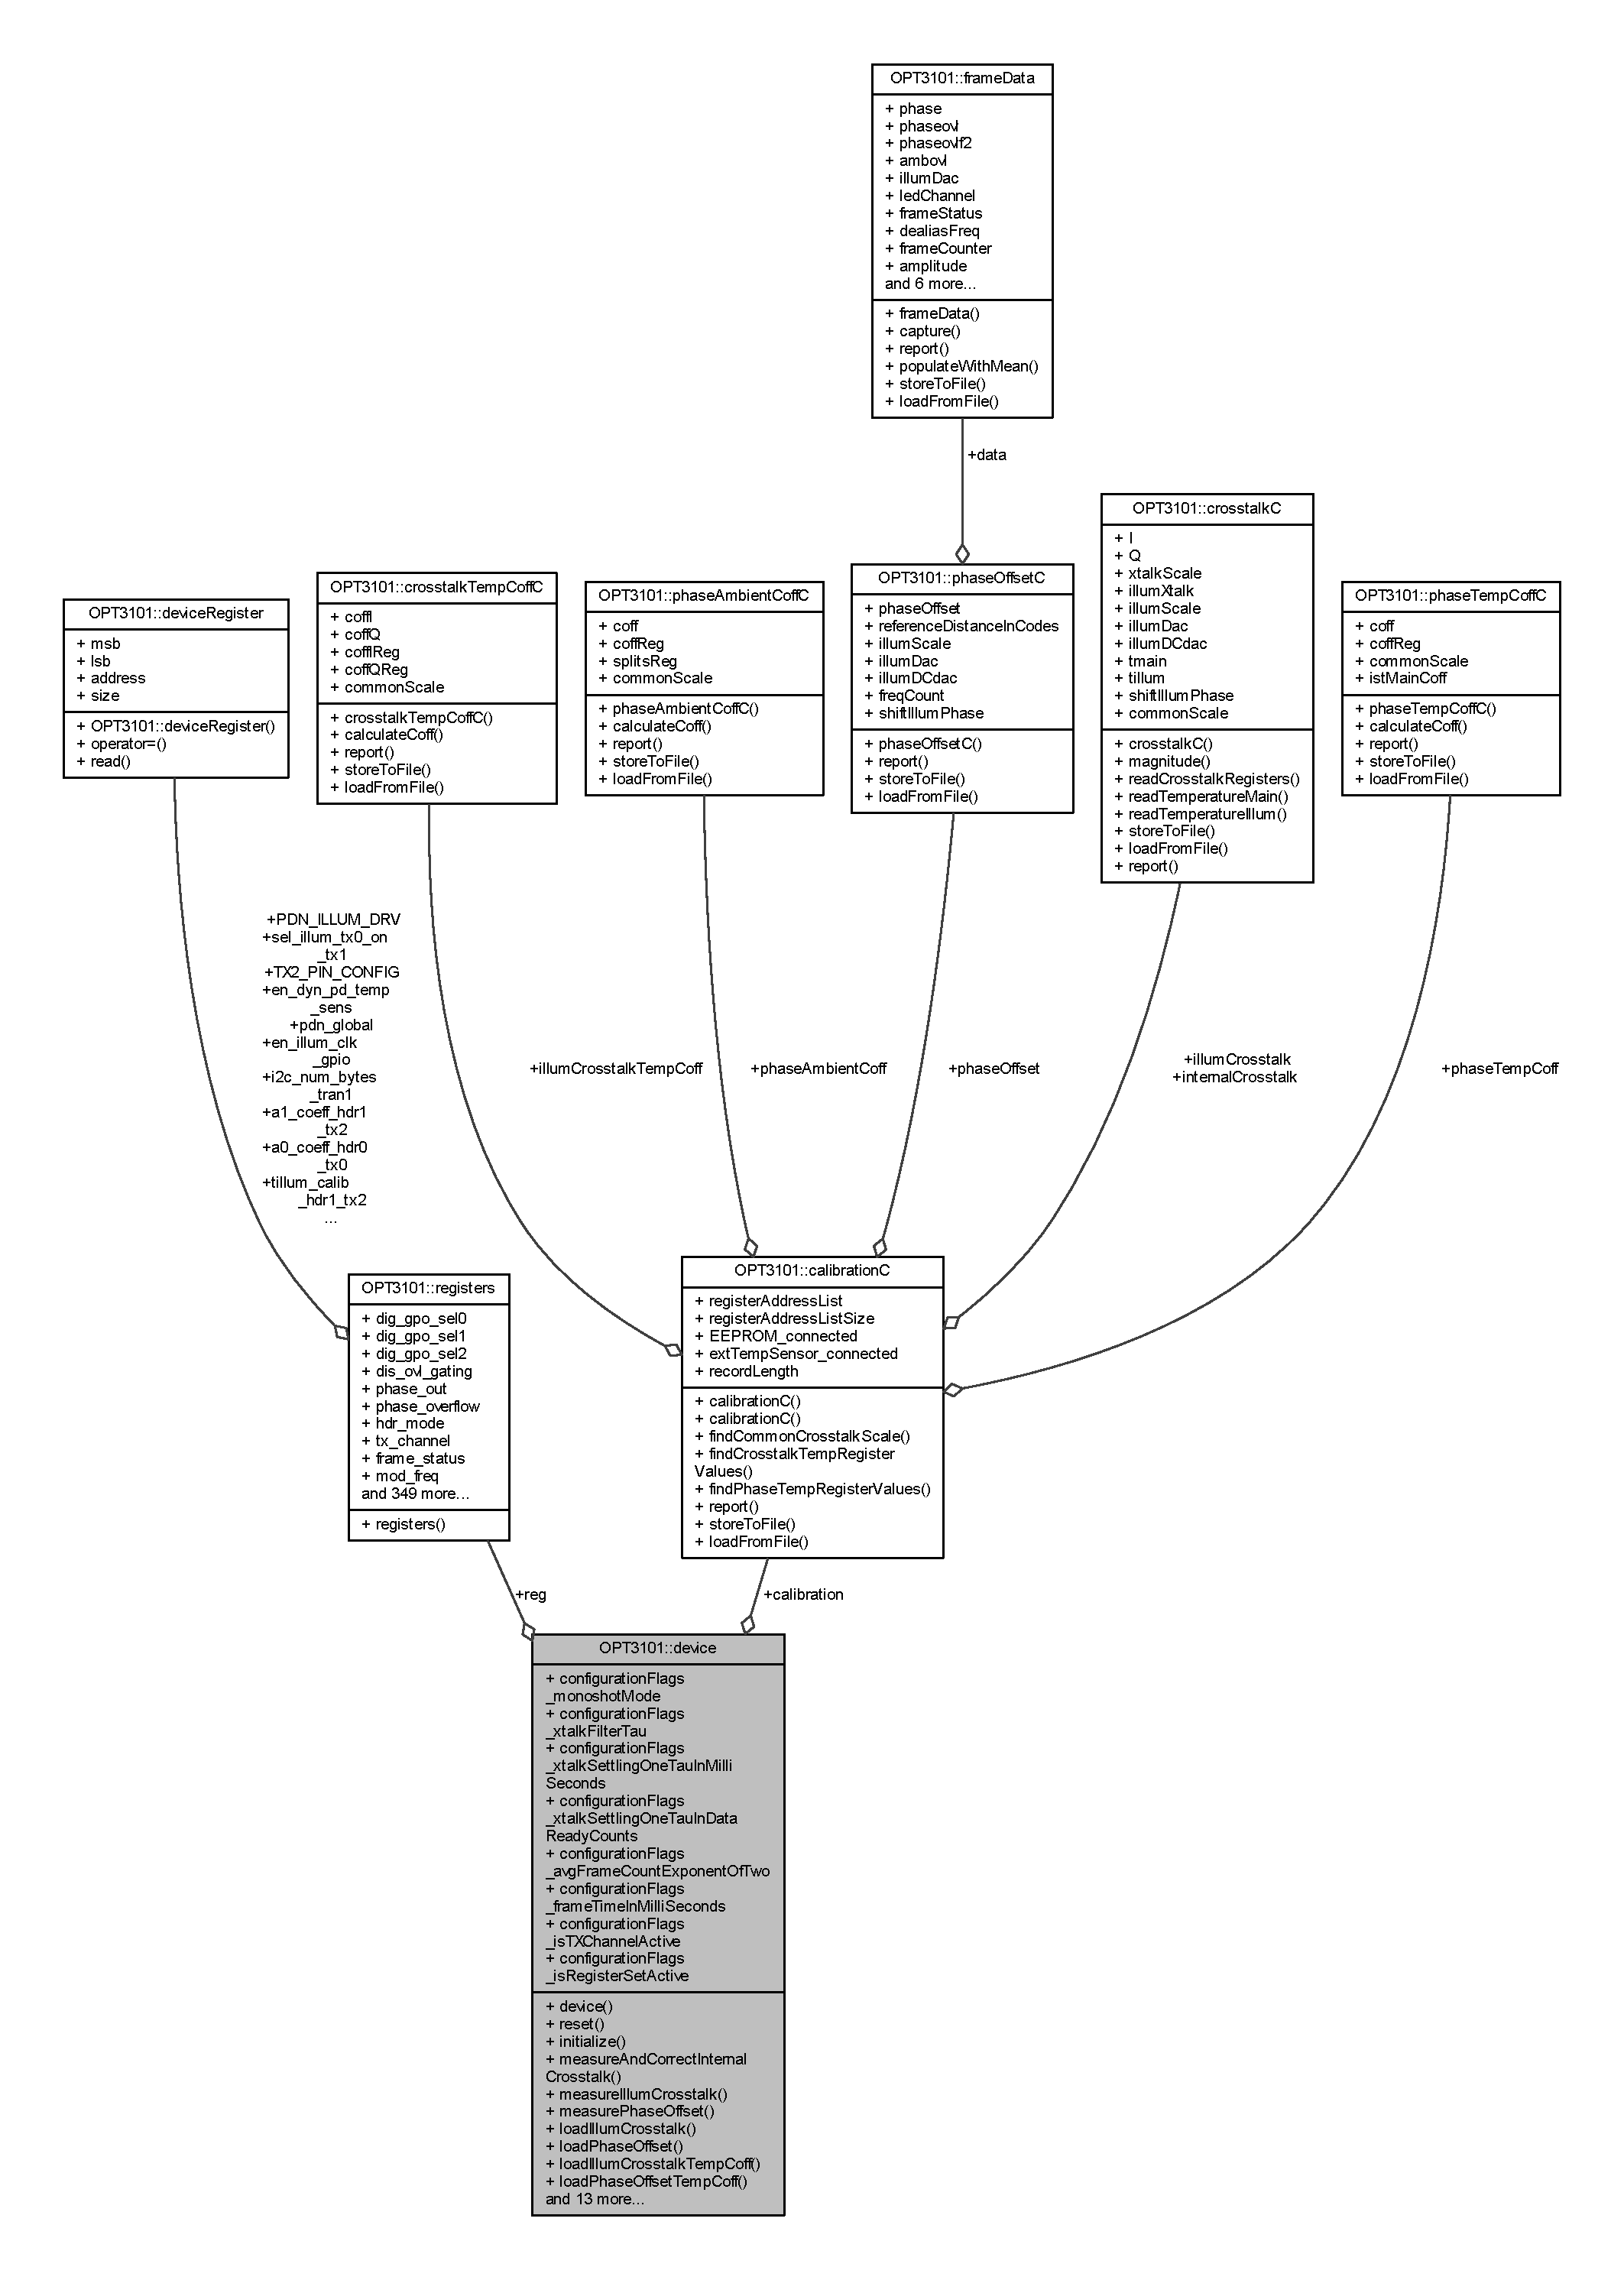
\includegraphics[width=350pt]{class_o_p_t3101_1_1device__coll__graph}
\end{center}
\end{figure}
\subsection*{Public Member Functions}
\begin{DoxyCompactItemize}
\item 
\mbox{\hyperlink{class_o_p_t3101_1_1device_a10acd9ff9c81c5d113d72a331ced450b}{device}} ()
\begin{DoxyCompactList}\small\item\em Constructor for class \mbox{\hyperlink{class_o_p_t3101_1_1device}{O\+P\+T3101\+::device}} Constructor definition for which is generated by \mbox{\hyperlink{namespace_o_p_t3101}{O\+P\+T3101}} configurator tool. Mainly the \mbox{\hyperlink{class_o_p_t3101_1_1device_aa911b5cc3747694d63c55a84b84dccd5}{O\+P\+T3101\+::device\+::configuration\+Flags\+\_\+is\+T\+X\+Channel\+Active}} and \mbox{\hyperlink{class_o_p_t3101_1_1device_a11813c9f13a5c970aa70d3318c4118b1}{O\+P\+T3101\+::device\+::configuration\+Flags\+\_\+is\+Register\+Set\+Active}} are set in the constructor. \end{DoxyCompactList}\item 
void \mbox{\hyperlink{class_o_p_t3101_1_1device_a1d37b22f535d8130c7f24799f7fa3c33}{reset}} ()
\begin{DoxyCompactList}\small\item\em resets device Template function which involves \mbox{\hyperlink{classhost_controller_aa9f25eaf4a9bda5213c70ff91c261649}{host\+Controller\+::reset\+Device}} method \end{DoxyCompactList}\item 
void \mbox{\hyperlink{class_o_p_t3101_1_1device_ae3b7fb4f9a8f1dee330523e034aa9460}{initialize}} ()
\begin{DoxyCompactList}\small\item\em initializes the device Definition for the method is generated by the \mbox{\hyperlink{namespace_o_p_t3101}{O\+P\+T3101}} configuration generator tool. This method consists for all the register writes and sequences required to bring the device to desired operating condition \end{DoxyCompactList}\item 
void \mbox{\hyperlink{class_o_p_t3101_1_1device_a44f832d6edbfb26db079ddba4debfdba}{measure\+And\+Correct\+Internal\+Crosstalk}} (\mbox{\hyperlink{class_o_p_t3101_1_1crosstalk_c}{crosstalkC}} $\ast$internal\+Xtalk)
\begin{DoxyCompactList}\small\item\em Measures and corrects internal crosstalk Method abstracts the internal crosstalk measurement. There are bunch of steps and register read/writes involved to measure and correct internal crosstalk which this method handles. This method is recommended to be run every time after power-\/up. \end{DoxyCompactList}\item 
void \mbox{\hyperlink{class_o_p_t3101_1_1device_a839d95aec303413e322382ff9e2228d4}{measure\+Illum\+Crosstalk}} (\mbox{\hyperlink{class_o_p_t3101_1_1crosstalk_c}{crosstalkC}} $\ast$illum\+Xtalk, uint8\+\_\+t tx\+Channel, char register\+Set, uint8\+\_\+t shift\+Illum\+Phase=0)
\begin{DoxyCompactList}\small\item\em Measures illum crosstalk for a given channel and register set Method abstracts the illum crosstalk measurement. The measurement of illum crosstalk for a given channel and register set involves configuring the device with bunch of register writes and reads. This method abstracts the procedure to make it simple for users to adopt~\newline
 This calibration procedure demands a very specific target/environmental requirement. This method invokes the appropriate template method from the env\+Controller class. Users needs to implement the method which achieves the specific requirement. \end{DoxyCompactList}\item 
void \mbox{\hyperlink{class_o_p_t3101_1_1device_a711d9737370bed043a85ced752c8ebb5}{measure\+Phase\+Offset}} (\mbox{\hyperlink{class_o_p_t3101_1_1phase_offset_c}{phase\+OffsetC}} $\ast$phase\+Offset, uint8\+\_\+t tx\+Channel, char register\+Set, uint16\+\_\+t ref\+Distance\+In\+Codes, uint8\+\_\+t shift\+Illum\+Phase=0)
\begin{DoxyCompactList}\small\item\em Measures phase offset for a given channel and register set Method abstracts the phase offset measurement. The measurement of phase offset is for a given channel and register set involves configuring the device with bunch of register writes and reads. This method abstracts the procedure to make it simple for users to adopt~\newline
 This calibration procedure demands a very specific target/environmental requirement. This method invokes the appropriate template method from the env\+Controller class. Users needs to implement the method which achieves the specific requirement. \end{DoxyCompactList}\item 
void \mbox{\hyperlink{class_o_p_t3101_1_1device_acb915ffb10d3c725fe4a58f22d69d27d}{load\+Illum\+Crosstalk}} (\mbox{\hyperlink{class_o_p_t3101_1_1crosstalk_c}{crosstalkC}} $\ast$illum\+Xtalk, uint8\+\_\+t tx\+Channel, char register\+Set)
\begin{DoxyCompactList}\small\item\em load illum crosstalk from \mbox{\hyperlink{class_o_p_t3101_1_1crosstalk_c}{O\+P\+T3101\+::crosstalkC}} class to the h/w Method loads the registers from \mbox{\hyperlink{class_o_p_t3101_1_1crosstalk_c}{O\+P\+T3101\+::crosstalkC}} instance specified to the h/w to specified tx\+Channel and register\+Set \end{DoxyCompactList}\item 
void \mbox{\hyperlink{class_o_p_t3101_1_1device_a941591aefa8b4c9b7436ac8f216938ed}{load\+Phase\+Offset}} (\mbox{\hyperlink{class_o_p_t3101_1_1phase_offset_c}{phase\+OffsetC}} $\ast$phase\+Offset, uint8\+\_\+t tx\+Channel, char register\+Set)
\begin{DoxyCompactList}\small\item\em load phase offset from \mbox{\hyperlink{class_o_p_t3101_1_1phase_offset_c}{O\+P\+T3101\+::phase\+OffsetC}} class to the h/w Method loads the registers from \mbox{\hyperlink{class_o_p_t3101_1_1phase_offset_c}{O\+P\+T3101\+::phase\+OffsetC}} instance specified to the h/w to specified tx\+Channel and register\+Set \end{DoxyCompactList}\item 
void \mbox{\hyperlink{class_o_p_t3101_1_1device_a450bc6b5bcd3e6b232d4352229a2829c}{load\+Illum\+Crosstalk\+Temp\+Coff}} (\mbox{\hyperlink{class_o_p_t3101_1_1crosstalk_temp_coff_c}{crosstalk\+Temp\+CoffC}} $\ast$illum\+Xtalk\+Temp\+Coff, uint8\+\_\+t tx\+Channel, char register\+Set)
\begin{DoxyCompactList}\small\item\em load crosstalk temperature coefficients from \mbox{\hyperlink{class_o_p_t3101_1_1crosstalk_temp_coff_c}{O\+P\+T3101\+::crosstalk\+Temp\+CoffC}} class to the h/w Method loads the registers from \mbox{\hyperlink{class_o_p_t3101_1_1crosstalk_temp_coff_c}{O\+P\+T3101\+::crosstalk\+Temp\+CoffC}} instance specified to the h/w to specified tx\+Channel and register\+Set \end{DoxyCompactList}\item 
void \mbox{\hyperlink{class_o_p_t3101_1_1device_a71e7ec6f26d54ea7cba11bf1c4132489}{load\+Phase\+Offset\+Temp\+Coff}} (\mbox{\hyperlink{class_o_p_t3101_1_1phase_temp_coff_c}{phase\+Temp\+CoffC}} $\ast$phase\+Temp\+Coff, uint8\+\_\+t tx\+Channel, char register\+Set)
\begin{DoxyCompactList}\small\item\em load phase offset temperature coefficients from \mbox{\hyperlink{class_o_p_t3101_1_1phase_temp_coff_c}{O\+P\+T3101\+::phase\+Temp\+CoffC}} class to the h/w Method loads the registers from \mbox{\hyperlink{class_o_p_t3101_1_1phase_temp_coff_c}{O\+P\+T3101\+::phase\+Temp\+CoffC}} instance specified to the h/w to specified tx\+Channel and register\+Set \end{DoxyCompactList}\item 
void \mbox{\hyperlink{class_o_p_t3101_1_1device_aa34206319a66be86de29789a1c24e3f7}{load\+Phase\+Ambient\+Coff}} (\mbox{\hyperlink{class_o_p_t3101_1_1phase_ambient_coff_c}{phase\+Ambient\+CoffC}} $\ast$phase\+Ambient\+Coff)
\begin{DoxyCompactList}\small\item\em load phase ambient coefficients from \mbox{\hyperlink{class_o_p_t3101_1_1phase_ambient_coff_c}{O\+P\+T3101\+::phase\+Ambient\+CoffC}} class to the h/w Method loads the registers from O\+P\+T3101\+::phase\+Ambient\+Coff instance specified to the h/w \end{DoxyCompactList}\item 
void \mbox{\hyperlink{class_o_p_t3101_1_1device_a48b320dfe4376bf62043d10ba937e8cd}{load\+Illum\+Crosstalk\+Set}} (bool load\+From\+File=true)
\begin{DoxyCompactList}\small\item\em loads all illum crosstalk set specified by \mbox{\hyperlink{namespace_o_p_t3101}{O\+P\+T3101}} configuration tool to h/w Method loads all the illum crosstalk registers from \mbox{\hyperlink{class_o_p_t3101_1_1calibration_c_ac09121c7057093506de63d6e2ea3a4b7}{O\+P\+T3101\+::calibration\+C\+::illum\+Crosstalk}} to the h/w to their specific TX channels and register sets. The order in which data is stored and indexed is preset and loaded accordingly. The method provides a higher level of abstraction for users to just load the illum\+Crosstalk calibration portion of the calibration data from the self contained instance of \mbox{\hyperlink{class_o_p_t3101_1_1calibration_c}{O\+P\+T3101\+::calibrationC}} to the h/w \end{DoxyCompactList}\item 
void \mbox{\hyperlink{class_o_p_t3101_1_1device_ab384cacd80cd32643b7029fe59428e92}{load\+Illum\+Crosstalk\+Temp\+Coff\+Set}} (bool load\+From\+File=true)
\begin{DoxyCompactList}\small\item\em loads all illum crosstalk temp coefficients set specified by \mbox{\hyperlink{namespace_o_p_t3101}{O\+P\+T3101}} configuration tool to h/w Method loads all the illum crosstalk temp coff registers from \mbox{\hyperlink{class_o_p_t3101_1_1calibration_c_ac7bcc22317965bb378479fb016c20d3c}{O\+P\+T3101\+::calibration\+C\+::illum\+Crosstalk\+Temp\+Coff}} to the h/w to their specific TX channels and register sets. The order in which data is stored and indexed is preset and loaded accordingly. The method provides a higher level of abstraction for users to just load the illum\+Crosstalk temp coff calibration portion of the calibration data from the self contained instance of \mbox{\hyperlink{class_o_p_t3101_1_1calibration_c}{O\+P\+T3101\+::calibrationC}} to the h/w \end{DoxyCompactList}\item 
void \mbox{\hyperlink{class_o_p_t3101_1_1device_a9fed055b5998d93bd37f26388ec8b0a8}{load\+Phase\+Offset\+Set}} ()
\begin{DoxyCompactList}\small\item\em loads all phase offset set specified by \mbox{\hyperlink{namespace_o_p_t3101}{O\+P\+T3101}} configuration tool to h/w Method loads all the phase offset registers from O\+P\+T3101\+::calibration\+::phase\+Offset to the h/w to their specific TX channels and register sets. The order in which data is stored and indexed is preset and loaded accordingly. The method provides a higher level of abstraction for users to just load the phase offset calibration portion of the calibration data from the self contained instance of \mbox{\hyperlink{class_o_p_t3101_1_1calibration_c}{O\+P\+T3101\+::calibrationC}} to the h/w \end{DoxyCompactList}\item 
void \mbox{\hyperlink{class_o_p_t3101_1_1device_a69d7fbb471d186845242774d7f2c86a8}{load\+Phase\+Offset\+Temp\+Coff\+Set}} (bool load\+From\+File=true)
\begin{DoxyCompactList}\small\item\em loads all phase temp coff set specified by \mbox{\hyperlink{namespace_o_p_t3101}{O\+P\+T3101}} configuration tool to h/w Method loads all the phase temp coff registers from O\+P\+T3101\+::calibration\+::phase\+Temp\+Coff to the h/w to their specific TX channels and register sets. The order in which data is stored and indexed is preset and loaded accordingly. The method provides a higher level of abstraction for users to just load the phase temp coff calibration portion of the calibration data from the self contained instance of \mbox{\hyperlink{class_o_p_t3101_1_1calibration_c}{O\+P\+T3101\+::calibrationC}} to the h/w \end{DoxyCompactList}\item 
void \mbox{\hyperlink{class_o_p_t3101_1_1device_ac70129fa0dacd700b19349087f000f76}{load\+Phase\+Ambient\+Coff\+Set}} (bool load\+From\+File=true)
\begin{DoxyCompactList}\small\item\em loads phase ambient coff set to h/w Method loads all the phase ambient coff registers from \mbox{\hyperlink{class_o_p_t3101_1_1calibration_c_ab69d912cc3cad353abeb73d7a95b7428}{O\+P\+T3101\+::calibration\+C\+::phase\+Ambient\+Coff}} to the h/w. The method provides a higher level of abstraction for users to just load the phase ambient coff calibration portion of the calibration data from the self contained instance of \mbox{\hyperlink{class_o_p_t3101_1_1calibration_c}{O\+P\+T3101\+::calibrationC}} to the h/w \end{DoxyCompactList}\item 
void \mbox{\hyperlink{class_o_p_t3101_1_1device_a0dd8c59bc93c392f8d3f430697457415}{calibration\+Session\+\_\+first\+Time\+Bring\+Up}} ()
\begin{DoxyCompactList}\small\item\em method for calibration session run the first time the board is brought up Method is a sequence of steps recommended when the system is powered up for the first time. This this is a session, this is a standalone session includes reset of device and initialization Details of the steps performed are documented in the detailed section \end{DoxyCompactList}\item 
void \mbox{\hyperlink{class_o_p_t3101_1_1device_a6b44ee9769ae8a2debff7b475bccdfe4}{calibration\+Session\+\_\+per\+Design\+Calibration\+Crosstalk\+Temp}} ()
\begin{DoxyCompactList}\small\item\em method for calibration of crosstalk temperature coefficients Method is a sequence of steps recommended to perform crosstalk temperature coefficients This this is a session, this is a standalone session includes reset of device and initialization Details of the steps performed are documented in the detailed section \end{DoxyCompactList}\item 
void \mbox{\hyperlink{class_o_p_t3101_1_1device_aec05fdf2f9780dea74305720ccb1cf32}{calibration\+Session\+\_\+per\+Design\+Calibration\+Phase\+Temp}} ()
\begin{DoxyCompactList}\small\item\em method for calibration of phase temperature coefficients This is recommended to be run on a few units per design. Coefficients calculated by this can be used for all the units in production Method is a sequence of steps recommended to perform phase temperature coefficients This this is a session, this is a standalone session includes reset of device and initialization Details of the steps performed are documented in the detailed section \end{DoxyCompactList}\item 
void \mbox{\hyperlink{class_o_p_t3101_1_1device_a94c4e35aa43bc53eb8fe0d4c364aea25}{calibration\+Session\+\_\+per\+Design\+Calibration\+Phase\+Ambient}} ()
\begin{DoxyCompactList}\small\item\em method for calibration of phase ambient coefficients This is recommended to be run on a few units per design. Coefficients calculated by this can be used for all the units in production Method is a sequence of steps recommended to perform phase ambient coefficients This this is a session, this is a standalone session includes reset of device and initialization Details of the steps performed are documented in the detailed section \end{DoxyCompactList}\item 
void \mbox{\hyperlink{class_o_p_t3101_1_1device_a3b278687f5414b66c614d83dcf229f80}{calibration\+\_\+per\+Design\+Calibration\+Phase\+Ambient\+Set\+Coff\+After\+Curve\+Fit}} ()
\begin{DoxyCompactList}\small\item\em method for calibration of phase ambient coefficients after manually curve fitting This is recommended to be run on a few units per design. Coefficients calculated by this can be used for all the units in production Method is a expected to be run after a P\+WL curve fit has been done to the ambient data after running \mbox{\hyperlink{class_o_p_t3101_1_1device_a94c4e35aa43bc53eb8fe0d4c364aea25}{O\+P\+T3101\+::device\+::calibration\+Session\+\_\+per\+Design\+Calibration\+Phase\+Ambient}} and analyzing and curve fitting the data This method doesn\textquotesingle{}t do anything to the device except to update the coff and store it to file Details of the steps performed are documented in the detailed section \end{DoxyCompactList}\item 
void \mbox{\hyperlink{class_o_p_t3101_1_1device_abad5b2d7405e735fa80041dbbf47502c}{calibration\+Session\+\_\+per\+Unit\+Factory\+Calibration}} ()
\begin{DoxyCompactList}\small\item\em method for calibration during factory for each unit of the system This is recommended to be run on a each and every units through production. Method is a sequence of steps recommended to perform all necessary calibration per unit This is a session, this is a standalone session includes reset of device and initialization Details of the steps performed are documented in the detailed section \end{DoxyCompactList}\item 
void \mbox{\hyperlink{class_o_p_t3101_1_1device_aa0a1b1f37d9aea753d7910de3e8c2799}{calibration\+Session\+\_\+per\+Unit\+Factory\+Calibration\+Write\+Register\+Data\+To\+Non\+Volatile\+Memory}} ()
\begin{DoxyCompactList}\small\item\em method to store the calibration to E\+E\+R\+P\+OM or some other from on non-\/volatile memory to be loaded on power-\/up every time This is recommended to be run on a each and every units through production after \mbox{\hyperlink{class_o_p_t3101_1_1device_abad5b2d7405e735fa80041dbbf47502c}{O\+P\+T3101\+::device\+::calibration\+Session\+\_\+per\+Unit\+Factory\+Calibration}} Method is a sequence of steps recommended to store the calibration data to a non-\/volatile memory for restoration during actual system operation In case if the configuration flag O\+P\+T3101\+::device\+::\+E\+E\+P\+R\+O\+M\+\_\+connected is set to true, this method uses the \mbox{\hyperlink{namespace_o_p_t3101}{O\+P\+T3101}} I2C slave to write data to the connected E\+E\+P\+R\+OM This is a session, this is a standalone session includes reset of device and initialization Details of the steps performed are documented in the detailed section \end{DoxyCompactList}\end{DoxyCompactItemize}
\subsection*{Public Attributes}
\begin{DoxyCompactItemize}
\item 
\mbox{\hyperlink{class_o_p_t3101_1_1registers}{registers}} \mbox{\hyperlink{class_o_p_t3101_1_1device_a0b36f012c21e9554a616c65ab3aa528b}{reg}}
\begin{DoxyCompactList}\small\item\em Instance of the register class \mbox{\hyperlink{class_o_p_t3101_1_1registers}{O\+P\+T3101\+::registers}} control for the device dev.\+reg.\{register\+Name\}=value initiates I2C register writes. \end{DoxyCompactList}\item 
\mbox{\hyperlink{class_o_p_t3101_1_1calibration_c}{calibrationC}} $\ast$ \mbox{\hyperlink{class_o_p_t3101_1_1device_a808c6e99f30fc4f21bee018f351f560d}{calibration}}
\begin{DoxyCompactList}\small\item\em Instance of the calibration class \mbox{\hyperlink{class_o_p_t3101_1_1calibration_c}{O\+P\+T3101\+::calibrationC}}. This instance acts a staging area to load, save and calculate calibration coefficients during initial bring up, debug and factory calibration steps. \end{DoxyCompactList}\item 
bool \mbox{\hyperlink{class_o_p_t3101_1_1device_a5ddd31b24f0caf9335ec8f8cc50584b2}{configuration\+Flags\+\_\+monoshot\+Mode}}
\begin{DoxyCompactList}\small\item\em Configuration flag to specify if the device is operating in mono shot mode which is set by \mbox{\hyperlink{namespace_o_p_t3101}{O\+P\+T3101}} configurator tool. \end{DoxyCompactList}\item 
uint8\+\_\+t \mbox{\hyperlink{class_o_p_t3101_1_1device_a93f398cf6cf57975f673afbab7ba9603}{configuration\+Flags\+\_\+xtalk\+Filter\+Tau}}
\begin{DoxyCompactList}\small\item\em Configuration value of crosstalk filter time constant which is set by \mbox{\hyperlink{namespace_o_p_t3101}{O\+P\+T3101}} configurator tool. \end{DoxyCompactList}\item 
uint16\+\_\+t \mbox{\hyperlink{class_o_p_t3101_1_1device_a9c579bc94d5a43a464129f5b67314eac}{configuration\+Flags\+\_\+xtalk\+Settling\+One\+Tau\+In\+Milli\+Seconds}}
\begin{DoxyCompactList}\small\item\em Configuration value specifying the time constant in milliseconds which is set by \mbox{\hyperlink{namespace_o_p_t3101}{O\+P\+T3101}} configurator tool. \end{DoxyCompactList}\item 
uint16\+\_\+t \mbox{\hyperlink{class_o_p_t3101_1_1device_acc3387f448c10f642260a031c5d0a11d}{configuration\+Flags\+\_\+xtalk\+Settling\+One\+Tau\+In\+Data\+Ready\+Counts}}
\begin{DoxyCompactList}\small\item\em Configuration value specifying the time constant in data ready counts which is set by \mbox{\hyperlink{namespace_o_p_t3101}{O\+P\+T3101}} configurator tool. \end{DoxyCompactList}\item 
uint8\+\_\+t \mbox{\hyperlink{class_o_p_t3101_1_1device_aa2216815a45a5641629331b10fd1ba2e}{configuration\+Flags\+\_\+avg\+Frame\+Count\+Exponent\+Of\+Two}}
\begin{DoxyCompactList}\small\item\em Configuration value specifying exponent component of average frame count which is set by \mbox{\hyperlink{namespace_o_p_t3101}{O\+P\+T3101}} configurator tool. \end{DoxyCompactList}\item 
uint32\+\_\+t \mbox{\hyperlink{class_o_p_t3101_1_1device_a5937bcbfb43b103d19b89285314f1351}{configuration\+Flags\+\_\+frame\+Time\+In\+Milli\+Seconds}}
\begin{DoxyCompactList}\small\item\em Configuration value specifying frame time in milli-\/seconds which is set by \mbox{\hyperlink{namespace_o_p_t3101}{O\+P\+T3101}} configurator tool. \end{DoxyCompactList}\item 
bool \mbox{\hyperlink{class_o_p_t3101_1_1device_aa911b5cc3747694d63c55a84b84dccd5}{configuration\+Flags\+\_\+is\+T\+X\+Channel\+Active}} \mbox{[}3\mbox{]}
\begin{DoxyCompactList}\small\item\em Configuration value specifying the active channels set by \mbox{\hyperlink{namespace_o_p_t3101}{O\+P\+T3101}} congifigurator tool. \end{DoxyCompactList}\item 
bool \mbox{\hyperlink{class_o_p_t3101_1_1device_a11813c9f13a5c970aa70d3318c4118b1}{configuration\+Flags\+\_\+is\+Register\+Set\+Active}} \mbox{[}2\mbox{]}
\begin{DoxyCompactList}\small\item\em Configuration value specifying the active register set by \mbox{\hyperlink{namespace_o_p_t3101}{O\+P\+T3101}} congifigurator tool. \end{DoxyCompactList}\end{DoxyCompactItemize}


\subsection{Detailed Description}
This is the master class that integrates all the O\+P\+T3101\+S\+DK functions. 

\mbox{\hyperlink{class_o_p_t3101_1_1device}{O\+P\+T3101\+::device}} is at the apex of the O\+P\+T3101\+S\+DK providing all the methods and functionality required for a full system bring up calibration and debug~\newline
 The register control for the device, calibration routines are instantiated in this call for user assess. 

\subsection{Constructor \& Destructor Documentation}
\mbox{\Hypertarget{class_o_p_t3101_1_1device_a10acd9ff9c81c5d113d72a331ced450b}\label{class_o_p_t3101_1_1device_a10acd9ff9c81c5d113d72a331ced450b}} 
\index{O\+P\+T3101\+::device@{O\+P\+T3101\+::device}!device@{device}}
\index{device@{device}!O\+P\+T3101\+::device@{O\+P\+T3101\+::device}}
\subsubsection{\texorpdfstring{device()}{device()}}
{\footnotesize\ttfamily O\+P\+T3101\+::device\+::device (\begin{DoxyParamCaption}{ }\end{DoxyParamCaption})}



Constructor for class \mbox{\hyperlink{class_o_p_t3101_1_1device}{O\+P\+T3101\+::device}} Constructor definition for which is generated by \mbox{\hyperlink{namespace_o_p_t3101}{O\+P\+T3101}} configurator tool. Mainly the \mbox{\hyperlink{class_o_p_t3101_1_1device_aa911b5cc3747694d63c55a84b84dccd5}{O\+P\+T3101\+::device\+::configuration\+Flags\+\_\+is\+T\+X\+Channel\+Active}} and \mbox{\hyperlink{class_o_p_t3101_1_1device_a11813c9f13a5c970aa70d3318c4118b1}{O\+P\+T3101\+::device\+::configuration\+Flags\+\_\+is\+Register\+Set\+Active}} are set in the constructor. 

\begin{DoxyReturn}{Returns}
Nothing; 
\end{DoxyReturn}


\subsection{Member Function Documentation}
\mbox{\Hypertarget{class_o_p_t3101_1_1device_a3b278687f5414b66c614d83dcf229f80}\label{class_o_p_t3101_1_1device_a3b278687f5414b66c614d83dcf229f80}} 
\index{O\+P\+T3101\+::device@{O\+P\+T3101\+::device}!calibration\+\_\+per\+Design\+Calibration\+Phase\+Ambient\+Set\+Coff\+After\+Curve\+Fit@{calibration\+\_\+per\+Design\+Calibration\+Phase\+Ambient\+Set\+Coff\+After\+Curve\+Fit}}
\index{calibration\+\_\+per\+Design\+Calibration\+Phase\+Ambient\+Set\+Coff\+After\+Curve\+Fit@{calibration\+\_\+per\+Design\+Calibration\+Phase\+Ambient\+Set\+Coff\+After\+Curve\+Fit}!O\+P\+T3101\+::device@{O\+P\+T3101\+::device}}
\subsubsection{\texorpdfstring{calibration\+\_\+per\+Design\+Calibration\+Phase\+Ambient\+Set\+Coff\+After\+Curve\+Fit()}{calibration\_perDesignCalibrationPhaseAmbientSetCoffAfterCurveFit()}}
{\footnotesize\ttfamily void O\+P\+T3101\+::device\+::calibration\+\_\+per\+Design\+Calibration\+Phase\+Ambient\+Set\+Coff\+After\+Curve\+Fit (\begin{DoxyParamCaption}{ }\end{DoxyParamCaption})}



method for calibration of phase ambient coefficients after manually curve fitting This is recommended to be run on a few units per design. Coefficients calculated by this can be used for all the units in production Method is a expected to be run after a P\+WL curve fit has been done to the ambient data after running \mbox{\hyperlink{class_o_p_t3101_1_1device_a94c4e35aa43bc53eb8fe0d4c364aea25}{O\+P\+T3101\+::device\+::calibration\+Session\+\_\+per\+Design\+Calibration\+Phase\+Ambient}} and analyzing and curve fitting the data This method doesn\textquotesingle{}t do anything to the device except to update the coff and store it to file Details of the steps performed are documented in the detailed section 

\begin{DoxyReturn}{Returns}
Nothing; 
\end{DoxyReturn}

\begin{DoxyItemize}
\item {\bfseries Warning\+:} User is expected to curve fit the phase ambient data with P\+WL curve fit and provide the floating point precision coefficients and split points ~\newline
~\newline
~\newline
~\newline

\item Creates filename phase\+Amb\+Coff.\+txt in path file\+Path
\item Users is expected to enter all the O\+P\+T3101\+::calibration\+::phase\+Ambient\+Coff\+::coff values manually after computation outside based on data generated by \mbox{\hyperlink{class_o_p_t3101_1_1device_a94c4e35aa43bc53eb8fe0d4c364aea25}{O\+P\+T3101\+::device\+::calibration\+Session\+\_\+per\+Design\+Calibration\+Phase\+Ambient}}
\item Users is expected to enter all the O\+P\+T3101\+::calibration\+::phase\+Ambient\+Coff\+::splits\+Reg values manually after computation outside based on data generated by \mbox{\hyperlink{class_o_p_t3101_1_1device_a94c4e35aa43bc53eb8fe0d4c364aea25}{O\+P\+T3101\+::device\+::calibration\+Session\+\_\+per\+Design\+Calibration\+Phase\+Ambient}}
\item Calls O\+P\+T3101\+::calibration\+::phase\+Ambient\+Coff\+::store\+To\+File to store to file name phase\+Amb\+Coff.\+txt in the path file\+Path 
\end{DoxyItemize}\mbox{\Hypertarget{class_o_p_t3101_1_1device_a0dd8c59bc93c392f8d3f430697457415}\label{class_o_p_t3101_1_1device_a0dd8c59bc93c392f8d3f430697457415}} 
\index{O\+P\+T3101\+::device@{O\+P\+T3101\+::device}!calibration\+Session\+\_\+first\+Time\+Bring\+Up@{calibration\+Session\+\_\+first\+Time\+Bring\+Up}}
\index{calibration\+Session\+\_\+first\+Time\+Bring\+Up@{calibration\+Session\+\_\+first\+Time\+Bring\+Up}!O\+P\+T3101\+::device@{O\+P\+T3101\+::device}}
\subsubsection{\texorpdfstring{calibration\+Session\+\_\+first\+Time\+Bring\+Up()}{calibrationSession\_firstTimeBringUp()}}
{\footnotesize\ttfamily void O\+P\+T3101\+::device\+::calibration\+Session\+\_\+first\+Time\+Bring\+Up (\begin{DoxyParamCaption}{ }\end{DoxyParamCaption})}



method for calibration session run the first time the board is brought up Method is a sequence of steps recommended when the system is powered up for the first time. This this is a session, this is a standalone session includes reset of device and initialization Details of the steps performed are documented in the detailed section 

\begin{DoxyReturn}{Returns}
Nothing; 
\end{DoxyReturn}
{\bfseries Algorithm of the method is as follows}


\begin{DoxyItemize}
\item Resets the device calling \mbox{\hyperlink{class_o_p_t3101_1_1device_a1d37b22f535d8130c7f24799f7fa3c33}{O\+P\+T3101\+::device\+::reset}} method
\item Initializes the \mbox{\hyperlink{namespace_o_p_t3101}{O\+P\+T3101}} device by calling \mbox{\hyperlink{class_o_p_t3101_1_1device_ae3b7fb4f9a8f1dee330523e034aa9460}{O\+P\+T3101\+::device\+::initialize}} method
\item Calls method \mbox{\hyperlink{class_o_p_t3101_1_1device_a44f832d6edbfb26db079ddba4debfdba}{O\+P\+T3101\+::device\+::measure\+And\+Correct\+Internal\+Crosstalk}} with argument \mbox{\hyperlink{class_o_p_t3101_1_1calibration_c_a4df5b876541e9b33eadf6290fe08b7e5}{O\+P\+T3101\+::calibration\+C\+::internal\+Crosstalk}}
\item Calls the method \mbox{\hyperlink{class_o_p_t3101_1_1crosstalk_c_a8a611602b13d6f3e97049696ddebe209}{O\+P\+T3101\+::crosstalk\+C\+::report}} for debug and data analysis
\item Calls the method \mbox{\hyperlink{classenvironmental_controller_a8a1fb44efff232844f00de18e174d4ce}{environmental\+Controller\+::set\+Target\+To\+Infinity\+\_\+\+O\+R\+\_\+cover\+Photodiode}} , which is expected to set the environment so as to be able to measure illumination crosstalk
\item Loops though all the valid TX channel and register set configurations
\item Calls method O\+P\+T3101\+::device\+::measure\+Illum\+Crosstalk with argument \mbox{\hyperlink{class_o_p_t3101_1_1calibration_c_ac09121c7057093506de63d6e2ea3a4b7}{O\+P\+T3101\+::calibration\+C\+::illum\+Crosstalk}}
\item Calls the method \mbox{\hyperlink{class_o_p_t3101_1_1crosstalk_c_a8a611602b13d6f3e97049696ddebe209}{O\+P\+T3101\+::crosstalk\+C\+::report}} for debug and data analysis
\item Creates filename illum\+Crosstalk\+\_\+\+TX\{channel\}\+\_\+\{h/l\}.txt in path file\+Path
\item Calls method \mbox{\hyperlink{class_o_p_t3101_1_1crosstalk_c_a7d887d736dd5a3aa9dd81224e67240b8}{O\+P\+T3101\+::crosstalk\+C\+::store\+To\+File}} to store the data 
\end{DoxyItemize}\mbox{\Hypertarget{class_o_p_t3101_1_1device_a6b44ee9769ae8a2debff7b475bccdfe4}\label{class_o_p_t3101_1_1device_a6b44ee9769ae8a2debff7b475bccdfe4}} 
\index{O\+P\+T3101\+::device@{O\+P\+T3101\+::device}!calibration\+Session\+\_\+per\+Design\+Calibration\+Crosstalk\+Temp@{calibration\+Session\+\_\+per\+Design\+Calibration\+Crosstalk\+Temp}}
\index{calibration\+Session\+\_\+per\+Design\+Calibration\+Crosstalk\+Temp@{calibration\+Session\+\_\+per\+Design\+Calibration\+Crosstalk\+Temp}!O\+P\+T3101\+::device@{O\+P\+T3101\+::device}}
\subsubsection{\texorpdfstring{calibration\+Session\+\_\+per\+Design\+Calibration\+Crosstalk\+Temp()}{calibrationSession\_perDesignCalibrationCrosstalkTemp()}}
{\footnotesize\ttfamily void O\+P\+T3101\+::device\+::calibration\+Session\+\_\+per\+Design\+Calibration\+Crosstalk\+Temp (\begin{DoxyParamCaption}{ }\end{DoxyParamCaption})}



method for calibration of crosstalk temperature coefficients Method is a sequence of steps recommended to perform crosstalk temperature coefficients This this is a session, this is a standalone session includes reset of device and initialization Details of the steps performed are documented in the detailed section 

\begin{DoxyReturn}{Returns}
Nothing; 
\end{DoxyReturn}
{\bfseries Algorithm of the method is as follows}


\begin{DoxyItemize}
\item Declares temporary variable of \mbox{\hyperlink{class_o_p_t3101_1_1crosstalk_c}{O\+P\+T3101\+::crosstalkC}} class to hold internal crosstalk data across temperature, TX channel and register settings
\item Resets the device calling \mbox{\hyperlink{class_o_p_t3101_1_1device_a1d37b22f535d8130c7f24799f7fa3c33}{O\+P\+T3101\+::device\+::reset}} method
\item Initializes the \mbox{\hyperlink{namespace_o_p_t3101}{O\+P\+T3101}} device by calling \mbox{\hyperlink{class_o_p_t3101_1_1device_ae3b7fb4f9a8f1dee330523e034aa9460}{O\+P\+T3101\+::device\+::initialize}} method
\item Calls method \mbox{\hyperlink{class_o_p_t3101_1_1device_a44f832d6edbfb26db079ddba4debfdba}{O\+P\+T3101\+::device\+::measure\+And\+Correct\+Internal\+Crosstalk}} with argument \mbox{\hyperlink{class_o_p_t3101_1_1calibration_c_a4df5b876541e9b33eadf6290fe08b7e5}{O\+P\+T3101\+::calibration\+C\+::internal\+Crosstalk}}
\item Calls the method \mbox{\hyperlink{classenvironmental_controller_a8a1fb44efff232844f00de18e174d4ce}{environmental\+Controller\+::set\+Target\+To\+Infinity\+\_\+\+O\+R\+\_\+cover\+Photodiode}} , which is expected to set the environment so as to be able to measure illumination crosstalk
\item Loops through chamber temperature settings to get temp coff
\item Calls the method \mbox{\hyperlink{classenvironmental_controller_a3c23e944f34f2d7c0fa0b279d5fc8a3f}{environmental\+Controller\+::set\+Chamber\+Temperature}} , which is expected to set the chamber to desired temperature
\item Loops though all the valid TX channel and register set configurations
\item Calls method O\+P\+T3101\+::device\+::measure\+Illum\+Crosstalk with temporary variable of \mbox{\hyperlink{class_o_p_t3101_1_1crosstalk_c}{O\+P\+T3101\+::crosstalkC}} class ~\newline
~\newline
~\newline
~\newline
~\newline
~\newline
~\newline

\item Creates filename illum\+Crosstalk\+\_\+\{chamber\+Temp\}C\+\_\+\+TX\{channel\}\+\_\+\{h/l\}.txt in path file\+Path
\item Calls method \mbox{\hyperlink{class_o_p_t3101_1_1crosstalk_c_a7d887d736dd5a3aa9dd81224e67240b8}{O\+P\+T3101\+::crosstalk\+C\+::store\+To\+File}} to store the data
\item Calls \mbox{\hyperlink{class_o_p_t3101_1_1crosstalk_c_a8a611602b13d6f3e97049696ddebe209}{O\+P\+T3101\+::crosstalk\+C\+::report}} method to report the crosstalk on screen
\item For each TX channel and register setting calls the \mbox{\hyperlink{class_o_p_t3101_1_1calibration_c_ac7bcc22317965bb378479fb016c20d3c}{O\+P\+T3101\+::calibration\+C\+::illum\+Crosstalk\+Temp\+Coff}} method with appropriate illum crosstalk values stored in temporary variable which stores calibration coeff to O\+P\+T3101\+::calibration\+::illum\+Crosstalk\+Temp\+Coff
\item Creates filename illum\+Crosstalk\+Temp\+Coff\+\_\+\+TX\{channel\}\+\_\+\{h/l\}.txt in path file\+Path
\item Calls method \mbox{\hyperlink{class_o_p_t3101_1_1crosstalk_temp_coff_c_aa24b81ff4f56b9f0f832b57086c87eb8}{O\+P\+T3101\+::crosstalk\+Temp\+Coff\+C\+::store\+To\+File}} to store the data
\item Calls \mbox{\hyperlink{class_o_p_t3101_1_1crosstalk_temp_coff_c_a881ec5ebe971af6c4c4f50e143d64f9a}{O\+P\+T3101\+::crosstalk\+Temp\+Coff\+C\+::report}} to report the crosstalk temp coff on screen 
\end{DoxyItemize}\mbox{\Hypertarget{class_o_p_t3101_1_1device_a94c4e35aa43bc53eb8fe0d4c364aea25}\label{class_o_p_t3101_1_1device_a94c4e35aa43bc53eb8fe0d4c364aea25}} 
\index{O\+P\+T3101\+::device@{O\+P\+T3101\+::device}!calibration\+Session\+\_\+per\+Design\+Calibration\+Phase\+Ambient@{calibration\+Session\+\_\+per\+Design\+Calibration\+Phase\+Ambient}}
\index{calibration\+Session\+\_\+per\+Design\+Calibration\+Phase\+Ambient@{calibration\+Session\+\_\+per\+Design\+Calibration\+Phase\+Ambient}!O\+P\+T3101\+::device@{O\+P\+T3101\+::device}}
\subsubsection{\texorpdfstring{calibration\+Session\+\_\+per\+Design\+Calibration\+Phase\+Ambient()}{calibrationSession\_perDesignCalibrationPhaseAmbient()}}
{\footnotesize\ttfamily void O\+P\+T3101\+::device\+::calibration\+Session\+\_\+per\+Design\+Calibration\+Phase\+Ambient (\begin{DoxyParamCaption}{ }\end{DoxyParamCaption})}



method for calibration of phase ambient coefficients This is recommended to be run on a few units per design. Coefficients calculated by this can be used for all the units in production Method is a sequence of steps recommended to perform phase ambient coefficients This this is a session, this is a standalone session includes reset of device and initialization Details of the steps performed are documented in the detailed section 

\begin{DoxyReturn}{Returns}
Nothing; 
\end{DoxyReturn}
{\bfseries Algorithm of the method is as follows}


\begin{DoxyItemize}
\item Resets the device calling \mbox{\hyperlink{class_o_p_t3101_1_1device_a1d37b22f535d8130c7f24799f7fa3c33}{O\+P\+T3101\+::device\+::reset}} method
\item Initializes the \mbox{\hyperlink{namespace_o_p_t3101}{O\+P\+T3101}} device by calling \mbox{\hyperlink{class_o_p_t3101_1_1device_ae3b7fb4f9a8f1dee330523e034aa9460}{O\+P\+T3101\+::device\+::initialize}} method
\item Calls method \mbox{\hyperlink{class_o_p_t3101_1_1device_a44f832d6edbfb26db079ddba4debfdba}{O\+P\+T3101\+::device\+::measure\+And\+Correct\+Internal\+Crosstalk}} with argument \mbox{\hyperlink{class_o_p_t3101_1_1calibration_c_a4df5b876541e9b33eadf6290fe08b7e5}{O\+P\+T3101\+::calibration\+C\+::internal\+Crosstalk}}
\item Calls method \mbox{\hyperlink{class_o_p_t3101_1_1device_a48b320dfe4376bf62043d10ba937e8cd}{O\+P\+T3101\+::device\+::load\+Illum\+Crosstalk\+Set}} to load all the illum crosstalk compensation registers
\item Loops though all the valid TX channel and register set configurations
\item {\bfseries Warning} User is expected to select and set reference distance so that the amplitude of the system for this particular TX and register set configurations measures between 16K and 24K. Default is set to 0 in the S\+DK
\item Calls \mbox{\hyperlink{classenvironmental_controller_a8251b7f25c6a6c5583c718bac664d05b}{environmental\+Controller\+::set\+Target\+Distance}} method with the specified distance
\item Converts the reference distance specified in codes related to \mbox{\hyperlink{class_o_p_t3101_1_1frame_data_af8661d11405953dc378ad4d7cb0f2db6}{O\+P\+T3101\+::frame\+Data\+::phase}} A\+DC codes
\item Loops through user desired ambient lux conditions to get phase Ambient coff
\item Calls the method \mbox{\hyperlink{classenvironmental_controller_adc63a8d9dbdbcef5768cf34692c6465c}{environmental\+Controller\+::set\+Ambient\+Light}} , which is expected to set the environment to have the specified ambient conditions
\item Measures phase offset by calling method O\+P\+T3101\+::device\+::measure\+Phase\+Offset with specified reference distance
\item Creates filename phase\+Amb\+Coff\+\_\+raw\+Data\+\_\+\{ambientin\+Lux\}lux.\+txt in path file\+Path
\item Calls \mbox{\hyperlink{class_o_p_t3101_1_1phase_offset_c_ae542e328ed54d6e791c1350d878d1dd0}{O\+P\+T3101\+::phase\+Offset\+C\+::store\+To\+File}} to archive the data for analysis and curve fitting
\item Calls \mbox{\hyperlink{class_o_p_t3101_1_1phase_offset_c_a6baba22699fdb39d45adfd104a44534c}{O\+P\+T3101\+::phase\+Offset\+C\+::report}} to display values on screen
\item Since Phase ambient coff is required to be done only for one TX configuration the the method breaks from the loop after 1 ambient sweep 
\end{DoxyItemize}\mbox{\Hypertarget{class_o_p_t3101_1_1device_aec05fdf2f9780dea74305720ccb1cf32}\label{class_o_p_t3101_1_1device_aec05fdf2f9780dea74305720ccb1cf32}} 
\index{O\+P\+T3101\+::device@{O\+P\+T3101\+::device}!calibration\+Session\+\_\+per\+Design\+Calibration\+Phase\+Temp@{calibration\+Session\+\_\+per\+Design\+Calibration\+Phase\+Temp}}
\index{calibration\+Session\+\_\+per\+Design\+Calibration\+Phase\+Temp@{calibration\+Session\+\_\+per\+Design\+Calibration\+Phase\+Temp}!O\+P\+T3101\+::device@{O\+P\+T3101\+::device}}
\subsubsection{\texorpdfstring{calibration\+Session\+\_\+per\+Design\+Calibration\+Phase\+Temp()}{calibrationSession\_perDesignCalibrationPhaseTemp()}}
{\footnotesize\ttfamily void O\+P\+T3101\+::device\+::calibration\+Session\+\_\+per\+Design\+Calibration\+Phase\+Temp (\begin{DoxyParamCaption}{ }\end{DoxyParamCaption})}



method for calibration of phase temperature coefficients This is recommended to be run on a few units per design. Coefficients calculated by this can be used for all the units in production Method is a sequence of steps recommended to perform phase temperature coefficients This this is a session, this is a standalone session includes reset of device and initialization Details of the steps performed are documented in the detailed section 

\begin{DoxyReturn}{Returns}
Nothing; 
\end{DoxyReturn}
{\bfseries Algorithm of the method is as follows}


\begin{DoxyItemize}
\item Declares temporary variable of \mbox{\hyperlink{class_o_p_t3101_1_1phase_offset_c}{O\+P\+T3101\+::phase\+OffsetC}} class to hold phase offset data across temperature, TX channel and register settings
\item Resets the device calling \mbox{\hyperlink{class_o_p_t3101_1_1device_a1d37b22f535d8130c7f24799f7fa3c33}{O\+P\+T3101\+::device\+::reset}} method
\item Initializes the \mbox{\hyperlink{namespace_o_p_t3101}{O\+P\+T3101}} device by calling \mbox{\hyperlink{class_o_p_t3101_1_1device_ae3b7fb4f9a8f1dee330523e034aa9460}{O\+P\+T3101\+::device\+::initialize}} method
\item Calls method \mbox{\hyperlink{class_o_p_t3101_1_1device_a44f832d6edbfb26db079ddba4debfdba}{O\+P\+T3101\+::device\+::measure\+And\+Correct\+Internal\+Crosstalk}} with argument \mbox{\hyperlink{class_o_p_t3101_1_1calibration_c_a4df5b876541e9b33eadf6290fe08b7e5}{O\+P\+T3101\+::calibration\+C\+::internal\+Crosstalk}}
\item Calls method \mbox{\hyperlink{class_o_p_t3101_1_1device_a48b320dfe4376bf62043d10ba937e8cd}{O\+P\+T3101\+::device\+::load\+Illum\+Crosstalk\+Set}} to load all the illum crosstalk compensation registers from files
\item Loops though all the valid TX channel and register set configurations
\item {\bfseries Warning} User is expected to select and set reference distance so that the amplitude of the system for this particular TX and register set configurations measures between 16K and 24K. Default is set to 0 in the S\+DK
\item Calls \mbox{\hyperlink{classenvironmental_controller_a8251b7f25c6a6c5583c718bac664d05b}{environmental\+Controller\+::set\+Target\+Distance}} method with the specified distance
\item Converts the reference distance specified in codes related to \mbox{\hyperlink{class_o_p_t3101_1_1frame_data_af8661d11405953dc378ad4d7cb0f2db6}{O\+P\+T3101\+::frame\+Data\+::phase}} A\+DC codes
\item Loops through chamber temperature settings to get temp coff
\item Calls the method \mbox{\hyperlink{classenvironmental_controller_a3c23e944f34f2d7c0fa0b279d5fc8a3f}{environmental\+Controller\+::set\+Chamber\+Temperature}} , which is expected to set the chamber to desired temperature
\item Measured phase offset by calling method O\+P\+T3101\+::device\+::measure\+Phase\+Offset with specified reference distance
\item Calls method \mbox{\hyperlink{class_o_p_t3101_1_1phase_temp_coff_c_a6a9ce25c87c81782b999e28c0a63a6af}{O\+P\+T3101\+::phase\+Temp\+Coff\+C\+::calculate\+Coff}} with temperature phase offset and assigns data to \mbox{\hyperlink{class_o_p_t3101_1_1calibration_c_a277a7bbf506f5f5181719311d10bc610}{O\+P\+T3101\+::calibration\+C\+::phase\+Temp\+Coff}}
\item Creates filename phase\+Temp\+Coff\+\_\+\+TX\{channel\}\+\_\+\{h/l\}.txt in path file\+Path
\item Calls method \mbox{\hyperlink{class_o_p_t3101_1_1phase_temp_coff_c_a05f0376e59830c4c81b37dc2042237e6}{O\+P\+T3101\+::phase\+Temp\+Coff\+C\+::store\+To\+File}} to store the data ~\newline

\item Calls \mbox{\hyperlink{class_o_p_t3101_1_1phase_temp_coff_c_af41bc218f81c9bfe8ae00e0bc6a64f4f}{O\+P\+T3101\+::phase\+Temp\+Coff\+C\+::report}} to report the phase temp coff on screen 
\end{DoxyItemize}\mbox{\Hypertarget{class_o_p_t3101_1_1device_abad5b2d7405e735fa80041dbbf47502c}\label{class_o_p_t3101_1_1device_abad5b2d7405e735fa80041dbbf47502c}} 
\index{O\+P\+T3101\+::device@{O\+P\+T3101\+::device}!calibration\+Session\+\_\+per\+Unit\+Factory\+Calibration@{calibration\+Session\+\_\+per\+Unit\+Factory\+Calibration}}
\index{calibration\+Session\+\_\+per\+Unit\+Factory\+Calibration@{calibration\+Session\+\_\+per\+Unit\+Factory\+Calibration}!O\+P\+T3101\+::device@{O\+P\+T3101\+::device}}
\subsubsection{\texorpdfstring{calibration\+Session\+\_\+per\+Unit\+Factory\+Calibration()}{calibrationSession\_perUnitFactoryCalibration()}}
{\footnotesize\ttfamily void O\+P\+T3101\+::device\+::calibration\+Session\+\_\+per\+Unit\+Factory\+Calibration (\begin{DoxyParamCaption}{ }\end{DoxyParamCaption})}



method for calibration during factory for each unit of the system This is recommended to be run on a each and every units through production. Method is a sequence of steps recommended to perform all necessary calibration per unit This is a session, this is a standalone session includes reset of device and initialization Details of the steps performed are documented in the detailed section 

\begin{DoxyReturn}{Returns}
Nothing; 
\end{DoxyReturn}
{\bfseries Algorithm of the method is as follows}


\begin{DoxyItemize}
\item Resets the device calling \mbox{\hyperlink{class_o_p_t3101_1_1device_a1d37b22f535d8130c7f24799f7fa3c33}{O\+P\+T3101\+::device\+::reset}} method
\item Initializes the \mbox{\hyperlink{namespace_o_p_t3101}{O\+P\+T3101}} device by calling \mbox{\hyperlink{class_o_p_t3101_1_1device_ae3b7fb4f9a8f1dee330523e034aa9460}{O\+P\+T3101\+::device\+::initialize}} method
\item Calls method \mbox{\hyperlink{class_o_p_t3101_1_1device_a44f832d6edbfb26db079ddba4debfdba}{O\+P\+T3101\+::device\+::measure\+And\+Correct\+Internal\+Crosstalk}} with argument \mbox{\hyperlink{class_o_p_t3101_1_1calibration_c_a4df5b876541e9b33eadf6290fe08b7e5}{O\+P\+T3101\+::calibration\+C\+::internal\+Crosstalk}}
\item Calls the method \mbox{\hyperlink{classenvironmental_controller_a8a1fb44efff232844f00de18e174d4ce}{environmental\+Controller\+::set\+Target\+To\+Infinity\+\_\+\+O\+R\+\_\+cover\+Photodiode}} , which is expected to set the environment so as to be able to measure illumination crosstalk
\item Loops though all the valid TX channel and register set configurations
\item Calls method O\+P\+T3101\+::device\+::measure\+Illum\+Crosstalk to capture the illumcrosstalk to variable \mbox{\hyperlink{class_o_p_t3101_1_1calibration_c_ac09121c7057093506de63d6e2ea3a4b7}{O\+P\+T3101\+::calibration\+C\+::illum\+Crosstalk}} for all TX config and register set
\item Calls \mbox{\hyperlink{class_o_p_t3101_1_1crosstalk_c_a8a611602b13d6f3e97049696ddebe209}{O\+P\+T3101\+::crosstalk\+C\+::report}} for each TX channel and register set to report crosstalk values on screen
\item Calls the \mbox{\hyperlink{class_o_p_t3101_1_1device_a48b320dfe4376bf62043d10ba937e8cd}{O\+P\+T3101\+::device\+::load\+Illum\+Crosstalk\+Set}} with false argument so that method to load all illum crosstalk settings from the O\+P\+T3101\+::device\+::crosstalk\+::illum\+Crosstalk member
\item Calls the \mbox{\hyperlink{class_o_p_t3101_1_1device_ab384cacd80cd32643b7029fe59428e92}{O\+P\+T3101\+::device\+::load\+Illum\+Crosstalk\+Temp\+Coff\+Set}} to load all illum crosstalk temp coff settings from file
\item Loops though all the valid TX channel and register set configurations
\item {\bfseries Warning} User is expected to select and set reference distance so that the amplitude of the system for this particular TX and register set configurations measures between 16K and 24K. Default is set to 0 in the S\+DK
\item Calls \mbox{\hyperlink{classenvironmental_controller_a8251b7f25c6a6c5583c718bac664d05b}{environmental\+Controller\+::set\+Target\+Distance}} method with the specified distance
\item Converts the reference distance specified in codes related to \mbox{\hyperlink{class_o_p_t3101_1_1frame_data_af8661d11405953dc378ad4d7cb0f2db6}{O\+P\+T3101\+::frame\+Data\+::phase}} A\+DC codes
\item Measures phase offset by calling method O\+P\+T3101\+::device\+::measure\+Phase\+Offset with specified reference distance and \mbox{\hyperlink{class_o_p_t3101_1_1calibration_c_a06f6a097057b9ed8f4914f4027d709c1}{O\+P\+T3101\+::calibration\+C\+::phase\+Offset}} as argument to store the phase offset values
\item Calls the \mbox{\hyperlink{class_o_p_t3101_1_1device_a69d7fbb471d186845242774d7f2c86a8}{O\+P\+T3101\+::device\+::load\+Phase\+Offset\+Temp\+Coff\+Set}} method to load all the phase offset temp coff. This method already calls O\+P\+T3101\+::load\+Phase\+Offset\+Set internally
\item Calls the \mbox{\hyperlink{class_o_p_t3101_1_1device_ac70129fa0dacd700b19349087f000f76}{O\+P\+T3101\+::device\+::load\+Phase\+Ambient\+Coff\+Set}} method to load all the phase offset temp coff
\item Calls the \mbox{\hyperlink{class_o_p_t3101_1_1device_aa0a1b1f37d9aea753d7910de3e8c2799}{O\+P\+T3101\+::device\+::calibration\+Session\+\_\+per\+Unit\+Factory\+Calibration\+Write\+Register\+Data\+To\+Non\+Volatile\+Memory}} to store the calibration data to a non-\/volatile memory 
\end{DoxyItemize}\mbox{\Hypertarget{class_o_p_t3101_1_1device_aa0a1b1f37d9aea753d7910de3e8c2799}\label{class_o_p_t3101_1_1device_aa0a1b1f37d9aea753d7910de3e8c2799}} 
\index{O\+P\+T3101\+::device@{O\+P\+T3101\+::device}!calibration\+Session\+\_\+per\+Unit\+Factory\+Calibration\+Write\+Register\+Data\+To\+Non\+Volatile\+Memory@{calibration\+Session\+\_\+per\+Unit\+Factory\+Calibration\+Write\+Register\+Data\+To\+Non\+Volatile\+Memory}}
\index{calibration\+Session\+\_\+per\+Unit\+Factory\+Calibration\+Write\+Register\+Data\+To\+Non\+Volatile\+Memory@{calibration\+Session\+\_\+per\+Unit\+Factory\+Calibration\+Write\+Register\+Data\+To\+Non\+Volatile\+Memory}!O\+P\+T3101\+::device@{O\+P\+T3101\+::device}}
\subsubsection{\texorpdfstring{calibration\+Session\+\_\+per\+Unit\+Factory\+Calibration\+Write\+Register\+Data\+To\+Non\+Volatile\+Memory()}{calibrationSession\_perUnitFactoryCalibrationWriteRegisterDataToNonVolatileMemory()}}
{\footnotesize\ttfamily void O\+P\+T3101\+::device\+::calibration\+Session\+\_\+per\+Unit\+Factory\+Calibration\+Write\+Register\+Data\+To\+Non\+Volatile\+Memory (\begin{DoxyParamCaption}{ }\end{DoxyParamCaption})}



method to store the calibration to E\+E\+R\+P\+OM or some other from on non-\/volatile memory to be loaded on power-\/up every time This is recommended to be run on a each and every units through production after \mbox{\hyperlink{class_o_p_t3101_1_1device_abad5b2d7405e735fa80041dbbf47502c}{O\+P\+T3101\+::device\+::calibration\+Session\+\_\+per\+Unit\+Factory\+Calibration}} Method is a sequence of steps recommended to store the calibration data to a non-\/volatile memory for restoration during actual system operation In case if the configuration flag O\+P\+T3101\+::device\+::\+E\+E\+P\+R\+O\+M\+\_\+connected is set to true, this method uses the \mbox{\hyperlink{namespace_o_p_t3101}{O\+P\+T3101}} I2C slave to write data to the connected E\+E\+P\+R\+OM This is a session, this is a standalone session includes reset of device and initialization Details of the steps performed are documented in the detailed section 

\begin{DoxyReturn}{Returns}
Nothing; 
\end{DoxyReturn}
{\bfseries Algorithm of the method is as follows}


\begin{DoxyItemize}
\item Method returns without doing any operation when the device configuration flag O\+P\+T3101\+::device\+::\+E\+E\+P\+R\+O\+M\+\_\+connected is false. User needs to implement their own function if no E\+E\+P\+R\+OM is present
\item Critical registers which are modified in this method are read from the h/w and temporarily bufferd to local variables.
\item \mbox{\hyperlink{namespace_o_p_t3101}{O\+P\+T3101}} device is configured to write desired data though the S\+D\+A\+\_\+\+M/\+S\+C\+L\+\_\+M lines to the connected external E\+E\+P\+R\+OM
\item Erases the E\+E\+P\+R\+OM with 0x\+FF data in all lcoations.
\item Reads all the registers from the list \mbox{\hyperlink{class_o_p_t3101_1_1calibration_c_a8ddd81159778cc987557c9b4920d5b57}{O\+P\+T3101\+::calibration\+C\+::register\+Address\+List}} from h/w and writes the address and data to the connected external E\+E\+P\+R\+OM
\item Restores the device state to the same state as before entering this method from the buffered local variables 
\end{DoxyItemize}\mbox{\Hypertarget{class_o_p_t3101_1_1device_ae3b7fb4f9a8f1dee330523e034aa9460}\label{class_o_p_t3101_1_1device_ae3b7fb4f9a8f1dee330523e034aa9460}} 
\index{O\+P\+T3101\+::device@{O\+P\+T3101\+::device}!initialize@{initialize}}
\index{initialize@{initialize}!O\+P\+T3101\+::device@{O\+P\+T3101\+::device}}
\subsubsection{\texorpdfstring{initialize()}{initialize()}}
{\footnotesize\ttfamily void O\+P\+T3101\+::device\+::initialize (\begin{DoxyParamCaption}{ }\end{DoxyParamCaption})}



initializes the device Definition for the method is generated by the \mbox{\hyperlink{namespace_o_p_t3101}{O\+P\+T3101}} configuration generator tool. This method consists for all the register writes and sequences required to bring the device to desired operating condition 

\begin{DoxyReturn}{Returns}
Nothing; 
\end{DoxyReturn}
$<$ \mbox{\Hypertarget{class_o_p_t3101_1_1device_acb915ffb10d3c725fe4a58f22d69d27d}\label{class_o_p_t3101_1_1device_acb915ffb10d3c725fe4a58f22d69d27d}} 
\index{O\+P\+T3101\+::device@{O\+P\+T3101\+::device}!load\+Illum\+Crosstalk@{load\+Illum\+Crosstalk}}
\index{load\+Illum\+Crosstalk@{load\+Illum\+Crosstalk}!O\+P\+T3101\+::device@{O\+P\+T3101\+::device}}
\subsubsection{\texorpdfstring{load\+Illum\+Crosstalk()}{loadIllumCrosstalk()}}
{\footnotesize\ttfamily void O\+P\+T3101\+::device\+::load\+Illum\+Crosstalk (\begin{DoxyParamCaption}\item[{\mbox{\hyperlink{class_o_p_t3101_1_1crosstalk_c}{O\+P\+T3101\+::crosstalkC}} $\ast$}]{illum\+Xtalk,  }\item[{uint8\+\_\+t}]{tx\+Channel,  }\item[{char}]{register\+Set }\end{DoxyParamCaption})}



load illum crosstalk from \mbox{\hyperlink{class_o_p_t3101_1_1crosstalk_c}{O\+P\+T3101\+::crosstalkC}} class to the h/w Method loads the registers from \mbox{\hyperlink{class_o_p_t3101_1_1crosstalk_c}{O\+P\+T3101\+::crosstalkC}} instance specified to the h/w to specified tx\+Channel and register\+Set 


\begin{DoxyParams}[1]{Parameters}
\mbox{\tt out}  & {\em illum\+Xtalk;} & illum\+Xtalk is pointer to the instance of \mbox{\hyperlink{class_o_p_t3101_1_1crosstalk_c}{O\+P\+T3101\+::crosstalkC}} class. The register values form the instance are loaded to the hardware to specified tx\+Channel and register\+Set \\
\hline
\mbox{\tt in}  & {\em tx\+Channel;} & tx\+Channel is the number denoting the channel to which the registers need to be loaded For eg\+: illum\+Xtalk=0 loads for T\+X0 channel \\
\hline
\mbox{\tt in}  & {\em register\+Set;} & register\+Set is a char \textquotesingle{}h\textquotesingle{} or \textquotesingle{}l\textquotesingle{} specifying register set on which register needs to be loaded. For eg\+: register\+Set=\textquotesingle{}h\textquotesingle{} would load on to registers related to illum\+\_\+dac\+\_\+h\+\_\+tx$\ast$ \\
\hline
\end{DoxyParams}
\begin{DoxyReturn}{Returns}
Nothing; 
\end{DoxyReturn}
{\bfseries Algorithm of the method is as follows}


\begin{DoxyItemize}
\item Load the common to all TX channels/register set registers (like for eg \mbox{\hyperlink{class_o_p_t3101_1_1registers_a92394965d2a4ebd5a540ae43a9a19403}{O\+P\+T3101\+::registers\+::illum\+\_\+xtalk\+\_\+reg\+\_\+scale}}) to the h/w from the method input argument illum\+Xtalk
\item Based on tx\+Channel and register\+Set argument the the method loads the \mbox{\hyperlink{class_o_p_t3101_1_1crosstalk_c_a97152b209288a0dc30c4158fdc1815fc}{O\+P\+T3101\+::crosstalk\+C\+::I}}, \mbox{\hyperlink{class_o_p_t3101_1_1crosstalk_c_a1e20d913baf2432ec90fe06a45c226db}{O\+P\+T3101\+::crosstalk\+C\+::Q}}, \mbox{\hyperlink{class_o_p_t3101_1_1crosstalk_c_a8b7250b531e953587c665c2c43860d82}{O\+P\+T3101\+::crosstalk\+C\+::tmain}} and \mbox{\hyperlink{class_o_p_t3101_1_1crosstalk_c_ab1d1d581f0495f5695ad49a2a8a41fd3}{O\+P\+T3101\+::crosstalk\+C\+::tillum}} to device h/w specified TX channels and register set ~\newline

\item for eg\+: then tx\+Channel=1 and register\+Set=\textquotesingle{}l\textquotesingle{} then the method loads the argument illum\+Xtalk\textquotesingle{}s \mbox{\hyperlink{class_o_p_t3101_1_1crosstalk_c_a97152b209288a0dc30c4158fdc1815fc}{O\+P\+T3101\+::crosstalk\+C\+::I}} to \mbox{\hyperlink{class_o_p_t3101_1_1registers_a897d8a5ef0a4d37b24e20276eb51a952}{O\+P\+T3101\+::registers\+::iphase\+\_\+xtalk\+\_\+reg\+\_\+hdr0\+\_\+tx1}} . Similarly the qphase\+\_\+reg$\ast$ registers, \mbox{\hyperlink{class_o_p_t3101_1_1registers_a68724aced807ba68873f5a6375bb611e}{O\+P\+T3101\+::registers\+::tmain\+\_\+calib\+\_\+hdr0\+\_\+tx1}} and \mbox{\hyperlink{class_o_p_t3101_1_1registers_aaa41e9820a7a006305ef538a8e3ac657}{O\+P\+T3101\+::registers\+::tillum\+\_\+calib\+\_\+hdr0\+\_\+tx1}} are loaded from the input argument illum\+Xtalk\textquotesingle{}s \mbox{\hyperlink{class_o_p_t3101_1_1crosstalk_c_a8b7250b531e953587c665c2c43860d82}{O\+P\+T3101\+::crosstalk\+C\+::tmain}} and \mbox{\hyperlink{class_o_p_t3101_1_1crosstalk_c_ab1d1d581f0495f5695ad49a2a8a41fd3}{O\+P\+T3101\+::crosstalk\+C\+::tillum}} 
\end{DoxyItemize}\mbox{\Hypertarget{class_o_p_t3101_1_1device_a48b320dfe4376bf62043d10ba937e8cd}\label{class_o_p_t3101_1_1device_a48b320dfe4376bf62043d10ba937e8cd}} 
\index{O\+P\+T3101\+::device@{O\+P\+T3101\+::device}!load\+Illum\+Crosstalk\+Set@{load\+Illum\+Crosstalk\+Set}}
\index{load\+Illum\+Crosstalk\+Set@{load\+Illum\+Crosstalk\+Set}!O\+P\+T3101\+::device@{O\+P\+T3101\+::device}}
\subsubsection{\texorpdfstring{load\+Illum\+Crosstalk\+Set()}{loadIllumCrosstalkSet()}}
{\footnotesize\ttfamily void O\+P\+T3101\+::device\+::load\+Illum\+Crosstalk\+Set (\begin{DoxyParamCaption}\item[{bool}]{load\+From\+File = {\ttfamily true} }\end{DoxyParamCaption})}



loads all illum crosstalk set specified by \mbox{\hyperlink{namespace_o_p_t3101}{O\+P\+T3101}} configuration tool to h/w Method loads all the illum crosstalk registers from \mbox{\hyperlink{class_o_p_t3101_1_1calibration_c_ac09121c7057093506de63d6e2ea3a4b7}{O\+P\+T3101\+::calibration\+C\+::illum\+Crosstalk}} to the h/w to their specific TX channels and register sets. The order in which data is stored and indexed is preset and loaded accordingly. The method provides a higher level of abstraction for users to just load the illum\+Crosstalk calibration portion of the calibration data from the self contained instance of \mbox{\hyperlink{class_o_p_t3101_1_1calibration_c}{O\+P\+T3101\+::calibrationC}} to the h/w 


\begin{DoxyParams}[1]{Parameters}
\mbox{\tt in}  & {\em load\+From\+File;} & load\+From\+File is a flag which specifies whether to load the calibration coff from file or from the \mbox{\hyperlink{class_o_p_t3101_1_1device_a808c6e99f30fc4f21bee018f351f560d}{O\+P\+T3101\+::device\+::calibration}} member of the \mbox{\hyperlink{class_o_p_t3101_1_1calibration_c}{O\+P\+T3101\+::calibrationC}} class \\
\hline
\end{DoxyParams}
\begin{DoxyReturn}{Returns}
Nothing; 
\end{DoxyReturn}
{\bfseries Algorithm of the method is as follows}


\begin{DoxyItemize}
\item Checks if input argument load\+From\+File is true. If true proceeds to load files in to \mbox{\hyperlink{class_o_p_t3101_1_1device_a808c6e99f30fc4f21bee018f351f560d}{O\+P\+T3101\+::device\+::calibration}}
\item Loops though all the valid TX channel and register set configurations
\item Calls method \mbox{\hyperlink{class_o_p_t3101_1_1crosstalk_c_a8927a7e31870bf41a64d8b1755c6b0b2}{O\+P\+T3101\+::crosstalk\+C\+::load\+From\+File}} to load data from non-\/volatile memory to all the O\+P\+T3101\+::device\+::calibration\+::illum\+Crosstalk members
\item Finds common crosstalk scale for the illum Crosstalk values captured in O\+P\+T3101\+::device\+::calibrationC using method \mbox{\hyperlink{class_o_p_t3101_1_1calibration_c_ae2c3f2786e65315d817b8953380e33b6}{O\+P\+T3101\+::calibration\+C\+::find\+Common\+Crosstalk\+Scale}}
\item Loops though all the valid TX channel and register set configurations
\item Loads all the illum crosstalk corresponding to TX and register set configurations to the device from the O\+P\+T3101\+::device\+::calibration\+C\+::illum\+Crosstalk member by calling \mbox{\hyperlink{class_o_p_t3101_1_1device_acb915ffb10d3c725fe4a58f22d69d27d}{O\+P\+T3101\+::device\+::load\+Illum\+Crosstalk}} 
\end{DoxyItemize}\mbox{\Hypertarget{class_o_p_t3101_1_1device_a450bc6b5bcd3e6b232d4352229a2829c}\label{class_o_p_t3101_1_1device_a450bc6b5bcd3e6b232d4352229a2829c}} 
\index{O\+P\+T3101\+::device@{O\+P\+T3101\+::device}!load\+Illum\+Crosstalk\+Temp\+Coff@{load\+Illum\+Crosstalk\+Temp\+Coff}}
\index{load\+Illum\+Crosstalk\+Temp\+Coff@{load\+Illum\+Crosstalk\+Temp\+Coff}!O\+P\+T3101\+::device@{O\+P\+T3101\+::device}}
\subsubsection{\texorpdfstring{load\+Illum\+Crosstalk\+Temp\+Coff()}{loadIllumCrosstalkTempCoff()}}
{\footnotesize\ttfamily void O\+P\+T3101\+::device\+::load\+Illum\+Crosstalk\+Temp\+Coff (\begin{DoxyParamCaption}\item[{\mbox{\hyperlink{class_o_p_t3101_1_1crosstalk_temp_coff_c}{O\+P\+T3101\+::crosstalk\+Temp\+CoffC}} $\ast$}]{illum\+Xtalk\+Temp\+Coff,  }\item[{uint8\+\_\+t}]{tx\+Channel,  }\item[{char}]{register\+Set }\end{DoxyParamCaption})}



load crosstalk temperature coefficients from \mbox{\hyperlink{class_o_p_t3101_1_1crosstalk_temp_coff_c}{O\+P\+T3101\+::crosstalk\+Temp\+CoffC}} class to the h/w Method loads the registers from \mbox{\hyperlink{class_o_p_t3101_1_1crosstalk_temp_coff_c}{O\+P\+T3101\+::crosstalk\+Temp\+CoffC}} instance specified to the h/w to specified tx\+Channel and register\+Set 


\begin{DoxyParams}[1]{Parameters}
\mbox{\tt in}  & {\em illum\+Xtalk\+Temp\+Coff;} & illum\+Xtalk\+Temp\+Coff is pointer to the instance of \mbox{\hyperlink{class_o_p_t3101_1_1crosstalk_temp_coff_c}{O\+P\+T3101\+::crosstalk\+Temp\+CoffC}} class. The register values form the instance are loaded to the hardware to specified tx\+Channel and register\+Set \\
\hline
\mbox{\tt in}  & {\em tx\+Channel;} & tx\+Channel is the number denoting the channel to which the registers need to be loaded For eg\+: illum\+Xtalk=0 loads for T\+X0 channel \\
\hline
\mbox{\tt in}  & {\em register\+Set;} & register\+Set is a char \textquotesingle{}h\textquotesingle{} or \textquotesingle{}l\textquotesingle{} specifying register set on which register needs to be loaded. For eg\+: register\+Set=\textquotesingle{}h\textquotesingle{} would load on to registers related to illum\+\_\+dac\+\_\+h\+\_\+tx$\ast$ \\
\hline
\end{DoxyParams}
\begin{DoxyReturn}{Returns}
Nothing; 
\end{DoxyReturn}
{\bfseries Algorithm of the method is as follows}


\begin{DoxyItemize}
\item loads common scale \mbox{\hyperlink{class_o_p_t3101_1_1crosstalk_temp_coff_c_a0ff621323b7f23672af224efca88e01e}{O\+P\+T3101\+::crosstalk\+Temp\+Coff\+C\+::common\+Scale}} from input argument illum\+Xtalk\+Temp\+Coff to device register \mbox{\hyperlink{class_o_p_t3101_1_1registers_a056d6a7717acab1d8915fc3977c0d130}{O\+P\+T3101\+::registers\+::scale\+\_\+temp\+\_\+coeff\+\_\+xtalk}}
\item Based on tx\+Channel and register\+Set argument the method loads the \mbox{\hyperlink{class_o_p_t3101_1_1crosstalk_temp_coff_c_a28ab8d4219f159782b1af029bd876cac}{O\+P\+T3101\+::crosstalk\+Temp\+Coff\+C\+::coff\+I\+Reg}} and \mbox{\hyperlink{class_o_p_t3101_1_1crosstalk_temp_coff_c_ae45f7932044d4d343f5f4d17ef0264c8}{O\+P\+T3101\+::crosstalk\+Temp\+Coff\+C\+::coff\+Q\+Reg}} to respective register set and channel registers ~\newline

\item for eg\+: then tx\+Channel=1 and register\+Set=\textquotesingle{}l\textquotesingle{} then the method loads the argument illum\+Xtalk\+Temp\+Coff\textquotesingle{}s \mbox{\hyperlink{class_o_p_t3101_1_1crosstalk_temp_coff_c_a28ab8d4219f159782b1af029bd876cac}{O\+P\+T3101\+::crosstalk\+Temp\+Coff\+C\+::coff\+I\+Reg}} to \mbox{\hyperlink{class_o_p_t3101_1_1registers_a2dff104599587cc06b51acc7dbf06270}{O\+P\+T3101\+::registers\+::temp\+\_\+coeff\+\_\+xtalk\+\_\+iphase\+\_\+hdr0\+\_\+tx1}} and similarly for the qphase register as well 
\end{DoxyItemize}\mbox{\Hypertarget{class_o_p_t3101_1_1device_ab384cacd80cd32643b7029fe59428e92}\label{class_o_p_t3101_1_1device_ab384cacd80cd32643b7029fe59428e92}} 
\index{O\+P\+T3101\+::device@{O\+P\+T3101\+::device}!load\+Illum\+Crosstalk\+Temp\+Coff\+Set@{load\+Illum\+Crosstalk\+Temp\+Coff\+Set}}
\index{load\+Illum\+Crosstalk\+Temp\+Coff\+Set@{load\+Illum\+Crosstalk\+Temp\+Coff\+Set}!O\+P\+T3101\+::device@{O\+P\+T3101\+::device}}
\subsubsection{\texorpdfstring{load\+Illum\+Crosstalk\+Temp\+Coff\+Set()}{loadIllumCrosstalkTempCoffSet()}}
{\footnotesize\ttfamily void O\+P\+T3101\+::device\+::load\+Illum\+Crosstalk\+Temp\+Coff\+Set (\begin{DoxyParamCaption}\item[{bool}]{load\+From\+File = {\ttfamily true} }\end{DoxyParamCaption})}



loads all illum crosstalk temp coefficients set specified by \mbox{\hyperlink{namespace_o_p_t3101}{O\+P\+T3101}} configuration tool to h/w Method loads all the illum crosstalk temp coff registers from \mbox{\hyperlink{class_o_p_t3101_1_1calibration_c_ac7bcc22317965bb378479fb016c20d3c}{O\+P\+T3101\+::calibration\+C\+::illum\+Crosstalk\+Temp\+Coff}} to the h/w to their specific TX channels and register sets. The order in which data is stored and indexed is preset and loaded accordingly. The method provides a higher level of abstraction for users to just load the illum\+Crosstalk temp coff calibration portion of the calibration data from the self contained instance of \mbox{\hyperlink{class_o_p_t3101_1_1calibration_c}{O\+P\+T3101\+::calibrationC}} to the h/w 


\begin{DoxyParams}[1]{Parameters}
\mbox{\tt in}  & {\em load\+From\+File;} & load\+From\+File is a flag which specifies whether to load the calibration coff from file or from the \mbox{\hyperlink{class_o_p_t3101_1_1device_a808c6e99f30fc4f21bee018f351f560d}{O\+P\+T3101\+::device\+::calibration}} member of the \mbox{\hyperlink{class_o_p_t3101_1_1calibration_c}{O\+P\+T3101\+::calibrationC}} class \\
\hline
\end{DoxyParams}
\begin{DoxyReturn}{Returns}
Nothing; 
\end{DoxyReturn}
{\bfseries Algorithm of the method is as follows}


\begin{DoxyItemize}
\item Check if the input flag to load from file is true. If True proceed to load from file... ~\newline
~\newline
~\newline
~\newline
~\newline
~\newline

\item Loops though all the valid TX channel and register set configurations
\item Loads from filename illum\+Crosstalk\+Temp\+Coff\+\_\+\+TX\{channel\}\+\_\+\{h/l\}.txt in path file\+Path using method \mbox{\hyperlink{class_o_p_t3101_1_1crosstalk_temp_coff_c_ae7028582197d0c77e9cf990dab888f1e}{O\+P\+T3101\+::crosstalk\+Temp\+Coff\+C\+::load\+From\+File}}
\item Calls \mbox{\hyperlink{class_o_p_t3101_1_1device_a48b320dfe4376bf62043d10ba937e8cd}{O\+P\+T3101\+::device\+::load\+Illum\+Crosstalk\+Set}} with the same loaf\+From\+File flag specified to this method ~\newline
~\newline
~\newline

\item Calls \mbox{\hyperlink{class_o_p_t3101_1_1calibration_c_ac133c41d60c71559a224a86bc3e62c3a}{O\+P\+T3101\+::calibration\+C\+::find\+Crosstalk\+Temp\+Register\+Values}} based on the members from \mbox{\hyperlink{class_o_p_t3101_1_1calibration_c}{O\+P\+T3101\+::calibrationC}} class \mbox{\hyperlink{class_o_p_t3101_1_1calibration_c_ac7bcc22317965bb378479fb016c20d3c}{O\+P\+T3101\+::calibration\+C\+::illum\+Crosstalk\+Temp\+Coff}} and \mbox{\hyperlink{class_o_p_t3101_1_1calibration_c_ac09121c7057093506de63d6e2ea3a4b7}{O\+P\+T3101\+::calibration\+C\+::illum\+Crosstalk}}
\item Loops though all the valid TX channel and register set configurations
\item Calls the method \mbox{\hyperlink{class_o_p_t3101_1_1device_a450bc6b5bcd3e6b232d4352229a2829c}{O\+P\+T3101\+::device\+::load\+Illum\+Crosstalk\+Temp\+Coff}} to load all the crosstalk temp coff values from the \mbox{\hyperlink{class_o_p_t3101_1_1calibration_c_ac7bcc22317965bb378479fb016c20d3c}{O\+P\+T3101\+::calibration\+C\+::illum\+Crosstalk\+Temp\+Coff}} member 
\end{DoxyItemize}\mbox{\Hypertarget{class_o_p_t3101_1_1device_aa34206319a66be86de29789a1c24e3f7}\label{class_o_p_t3101_1_1device_aa34206319a66be86de29789a1c24e3f7}} 
\index{O\+P\+T3101\+::device@{O\+P\+T3101\+::device}!load\+Phase\+Ambient\+Coff@{load\+Phase\+Ambient\+Coff}}
\index{load\+Phase\+Ambient\+Coff@{load\+Phase\+Ambient\+Coff}!O\+P\+T3101\+::device@{O\+P\+T3101\+::device}}
\subsubsection{\texorpdfstring{load\+Phase\+Ambient\+Coff()}{loadPhaseAmbientCoff()}}
{\footnotesize\ttfamily void O\+P\+T3101\+::device\+::load\+Phase\+Ambient\+Coff (\begin{DoxyParamCaption}\item[{\mbox{\hyperlink{class_o_p_t3101_1_1phase_ambient_coff_c}{O\+P\+T3101\+::phase\+Ambient\+CoffC}} $\ast$}]{phase\+Ambient\+Coff }\end{DoxyParamCaption})}



load phase ambient coefficients from \mbox{\hyperlink{class_o_p_t3101_1_1phase_ambient_coff_c}{O\+P\+T3101\+::phase\+Ambient\+CoffC}} class to the h/w Method loads the registers from O\+P\+T3101\+::phase\+Ambient\+Coff instance specified to the h/w 


\begin{DoxyParams}[1]{Parameters}
\mbox{\tt in}  & {\em phase\+Ambient\+Coff;} & phase\+Ambient\+Coff is pointer to the instance of \mbox{\hyperlink{class_o_p_t3101_1_1phase_ambient_coff_c}{O\+P\+T3101\+::phase\+Ambient\+CoffC}} class. The register values form the instance are loaded to the hardware \\
\hline
\end{DoxyParams}
\begin{DoxyReturn}{Returns}
Nothing; 
\end{DoxyReturn}
{\bfseries Algorithm of the method is as follows}


\begin{DoxyItemize}
\item Assigns all the register entries from phase\+Ambient\+Coff \mbox{\hyperlink{class_o_p_t3101_1_1phase_ambient_coff_c}{O\+P\+T3101\+::phase\+Ambient\+CoffC}} to h/w registers ~\newline

\item for eg\+: input argument phase\+Ambient\+Coff\textquotesingle{}s \mbox{\hyperlink{class_o_p_t3101_1_1phase_ambient_coff_c_a267c8f925dedeb8af97aba7ffae95da4}{O\+P\+T3101\+::phase\+Ambient\+Coff\+C\+::coff\+Reg}} is loaded to \mbox{\hyperlink{class_o_p_t3101_1_1registers_a3a959d073208e7bc1859551052620c33}{O\+P\+T3101\+::registers\+::amb\+\_\+phase\+\_\+corr\+\_\+pwl\+\_\+coeff0}} and other related registers 
\end{DoxyItemize}\mbox{\Hypertarget{class_o_p_t3101_1_1device_ac70129fa0dacd700b19349087f000f76}\label{class_o_p_t3101_1_1device_ac70129fa0dacd700b19349087f000f76}} 
\index{O\+P\+T3101\+::device@{O\+P\+T3101\+::device}!load\+Phase\+Ambient\+Coff\+Set@{load\+Phase\+Ambient\+Coff\+Set}}
\index{load\+Phase\+Ambient\+Coff\+Set@{load\+Phase\+Ambient\+Coff\+Set}!O\+P\+T3101\+::device@{O\+P\+T3101\+::device}}
\subsubsection{\texorpdfstring{load\+Phase\+Ambient\+Coff\+Set()}{loadPhaseAmbientCoffSet()}}
{\footnotesize\ttfamily void O\+P\+T3101\+::device\+::load\+Phase\+Ambient\+Coff\+Set (\begin{DoxyParamCaption}\item[{bool}]{load\+From\+File = {\ttfamily true} }\end{DoxyParamCaption})}



loads phase ambient coff set to h/w Method loads all the phase ambient coff registers from \mbox{\hyperlink{class_o_p_t3101_1_1calibration_c_ab69d912cc3cad353abeb73d7a95b7428}{O\+P\+T3101\+::calibration\+C\+::phase\+Ambient\+Coff}} to the h/w. The method provides a higher level of abstraction for users to just load the phase ambient coff calibration portion of the calibration data from the self contained instance of \mbox{\hyperlink{class_o_p_t3101_1_1calibration_c}{O\+P\+T3101\+::calibrationC}} to the h/w 


\begin{DoxyParams}[1]{Parameters}
\mbox{\tt in}  & {\em load\+From\+File;} & load\+From\+File is a flag which specifies whether to load the calibration coff from file or from the \mbox{\hyperlink{class_o_p_t3101_1_1device_a808c6e99f30fc4f21bee018f351f560d}{O\+P\+T3101\+::device\+::calibration}} member of the \mbox{\hyperlink{class_o_p_t3101_1_1calibration_c}{O\+P\+T3101\+::calibrationC}} class \\
\hline
\end{DoxyParams}
\begin{DoxyReturn}{Returns}
Nothing; 
\end{DoxyReturn}
{\bfseries Algorithm of the method is as follows}


\begin{DoxyItemize}
\item loads from filename phase\+Amb\+Coff.\+txt in path file\+Path
\item Calls \mbox{\hyperlink{class_o_p_t3101_1_1phase_ambient_coff_c_a41db9882facdbf3b437dcb54958b5763}{O\+P\+T3101\+::phase\+Ambient\+Coff\+C\+::load\+From\+File}} to load the coff from file to the \mbox{\hyperlink{class_o_p_t3101_1_1calibration_c_ab69d912cc3cad353abeb73d7a95b7428}{O\+P\+T3101\+::calibration\+C\+::phase\+Ambient\+Coff}} member
\item Calculates the phase ambient coff by calling method \mbox{\hyperlink{class_o_p_t3101_1_1phase_ambient_coff_c_ac8f4dfff191b0adc7be044f39500e242}{O\+P\+T3101\+::phase\+Ambient\+Coff\+C\+::calculate\+Coff}} also passing argument of device register \mbox{\hyperlink{class_o_p_t3101_1_1registers_a0d343738560c0bc418f34b458735a811}{O\+P\+T3101\+::registers\+::freq\+\_\+count\+\_\+read\+\_\+reg}}
\item Calls method \mbox{\hyperlink{class_o_p_t3101_1_1device_aa34206319a66be86de29789a1c24e3f7}{O\+P\+T3101\+::device\+::load\+Phase\+Ambient\+Coff}} to load ambient coff to device from \mbox{\hyperlink{class_o_p_t3101_1_1calibration_c_ab69d912cc3cad353abeb73d7a95b7428}{O\+P\+T3101\+::calibration\+C\+::phase\+Ambient\+Coff}} member 
\end{DoxyItemize}\mbox{\Hypertarget{class_o_p_t3101_1_1device_a941591aefa8b4c9b7436ac8f216938ed}\label{class_o_p_t3101_1_1device_a941591aefa8b4c9b7436ac8f216938ed}} 
\index{O\+P\+T3101\+::device@{O\+P\+T3101\+::device}!load\+Phase\+Offset@{load\+Phase\+Offset}}
\index{load\+Phase\+Offset@{load\+Phase\+Offset}!O\+P\+T3101\+::device@{O\+P\+T3101\+::device}}
\subsubsection{\texorpdfstring{load\+Phase\+Offset()}{loadPhaseOffset()}}
{\footnotesize\ttfamily void O\+P\+T3101\+::device\+::load\+Phase\+Offset (\begin{DoxyParamCaption}\item[{\mbox{\hyperlink{class_o_p_t3101_1_1phase_offset_c}{O\+P\+T3101\+::phase\+OffsetC}} $\ast$}]{phase\+Offset,  }\item[{uint8\+\_\+t}]{tx\+Channel,  }\item[{char}]{register\+Set }\end{DoxyParamCaption})}



load phase offset from \mbox{\hyperlink{class_o_p_t3101_1_1phase_offset_c}{O\+P\+T3101\+::phase\+OffsetC}} class to the h/w Method loads the registers from \mbox{\hyperlink{class_o_p_t3101_1_1phase_offset_c}{O\+P\+T3101\+::phase\+OffsetC}} instance specified to the h/w to specified tx\+Channel and register\+Set 


\begin{DoxyParams}[1]{Parameters}
\mbox{\tt in}  & {\em phase\+Offset;} & phase\+Offset is pointer to the instance of \mbox{\hyperlink{class_o_p_t3101_1_1phase_offset_c}{O\+P\+T3101\+::phase\+OffsetC}} class. The register values form the instance are loaded to the hardware to specified tx\+Channel and register\+Set \\
\hline
\mbox{\tt in}  & {\em tx\+Channel;} & tx\+Channel is the number denoting the channel to which the registers need to be loaded For eg\+: illum\+Xtalk=0 loads for T\+X0 channel \\
\hline
\mbox{\tt in}  & {\em register\+Set;} & register\+Set is a char \textquotesingle{}h\textquotesingle{} or \textquotesingle{}l\textquotesingle{} specifying register set on which register needs to be loaded. For eg\+: register\+Set=\textquotesingle{}h\textquotesingle{} would load on to registers related to illum\+\_\+dac\+\_\+h\+\_\+tx$\ast$ \\
\hline
\end{DoxyParams}
\begin{DoxyReturn}{Returns}
Nothing; 
\end{DoxyReturn}
{\bfseries Algorithm of the method is as follows}


\begin{DoxyItemize}
\item Enables the phase offset correction register \mbox{\hyperlink{class_o_p_t3101_1_1registers_a66984616af1af7f24eaf7226e8d64c11}{O\+P\+T3101\+::registers\+::en\+\_\+phase\+\_\+corr}}
\item Based on tx\+Channel and register\+Set argument the the method loads the \mbox{\hyperlink{class_o_p_t3101_1_1phase_offset_c_addeef913546f1c431b4fd189478884f9}{O\+P\+T3101\+::phase\+Offset\+C\+::phase\+Offset}}, O\+P\+T3101\+::phase\+Offset\+C\+::frame\+Data\+::tmain and O\+P\+T3101\+::phase\+Offset\+C\+::frame\+Data\+::tillum to device h/w specified TX channels and register set ~\newline

\item for eg\+: then tx\+Channel=1 and register\+Set=\textquotesingle{}l\textquotesingle{} then the method loads the argument phase\+Offset\textquotesingle{}s \mbox{\hyperlink{class_o_p_t3101_1_1phase_offset_c_addeef913546f1c431b4fd189478884f9}{O\+P\+T3101\+::phase\+Offset\+C\+::phase\+Offset}} to \mbox{\hyperlink{class_o_p_t3101_1_1registers_a4097670bfd34c50f64b7644626bb3390}{O\+P\+T3101\+::registers\+::phase\+\_\+offset\+\_\+hdr0\+\_\+tx1}} \mbox{\hyperlink{class_o_p_t3101_1_1registers_a68724aced807ba68873f5a6375bb611e}{O\+P\+T3101\+::registers\+::tmain\+\_\+calib\+\_\+hdr0\+\_\+tx1}} and \mbox{\hyperlink{class_o_p_t3101_1_1registers_aaa41e9820a7a006305ef538a8e3ac657}{O\+P\+T3101\+::registers\+::tillum\+\_\+calib\+\_\+hdr0\+\_\+tx1}} are loaded from the input argument phase\+Offset\textquotesingle{}s O\+P\+T3101\+::phase\+Offset\+C\+::frame\+Data\+::tmain and O\+P\+T3101\+::phase\+Offset\+C\+::frame\+Data\+::tillum 
\end{DoxyItemize}\mbox{\Hypertarget{class_o_p_t3101_1_1device_a9fed055b5998d93bd37f26388ec8b0a8}\label{class_o_p_t3101_1_1device_a9fed055b5998d93bd37f26388ec8b0a8}} 
\index{O\+P\+T3101\+::device@{O\+P\+T3101\+::device}!load\+Phase\+Offset\+Set@{load\+Phase\+Offset\+Set}}
\index{load\+Phase\+Offset\+Set@{load\+Phase\+Offset\+Set}!O\+P\+T3101\+::device@{O\+P\+T3101\+::device}}
\subsubsection{\texorpdfstring{load\+Phase\+Offset\+Set()}{loadPhaseOffsetSet()}}
{\footnotesize\ttfamily void O\+P\+T3101\+::device\+::load\+Phase\+Offset\+Set (\begin{DoxyParamCaption}{ }\end{DoxyParamCaption})}



loads all phase offset set specified by \mbox{\hyperlink{namespace_o_p_t3101}{O\+P\+T3101}} configuration tool to h/w Method loads all the phase offset registers from O\+P\+T3101\+::calibration\+::phase\+Offset to the h/w to their specific TX channels and register sets. The order in which data is stored and indexed is preset and loaded accordingly. The method provides a higher level of abstraction for users to just load the phase offset calibration portion of the calibration data from the self contained instance of \mbox{\hyperlink{class_o_p_t3101_1_1calibration_c}{O\+P\+T3101\+::calibrationC}} to the h/w 

\begin{DoxyReturn}{Returns}
Nothing; 
\end{DoxyReturn}
{\bfseries Algorithm of the method is as follows}


\begin{DoxyItemize}
\item Loops though all the valid TX channel and register set configurations
\item Loads all the phase offset corresponding to TX and register set configurations to the device from the O\+P\+T3101\+::device\+::calibration\+C\+::phase\+Offset member by calling \mbox{\hyperlink{class_o_p_t3101_1_1device_a941591aefa8b4c9b7436ac8f216938ed}{O\+P\+T3101\+::device\+::load\+Phase\+Offset}} 
\end{DoxyItemize}\mbox{\Hypertarget{class_o_p_t3101_1_1device_a71e7ec6f26d54ea7cba11bf1c4132489}\label{class_o_p_t3101_1_1device_a71e7ec6f26d54ea7cba11bf1c4132489}} 
\index{O\+P\+T3101\+::device@{O\+P\+T3101\+::device}!load\+Phase\+Offset\+Temp\+Coff@{load\+Phase\+Offset\+Temp\+Coff}}
\index{load\+Phase\+Offset\+Temp\+Coff@{load\+Phase\+Offset\+Temp\+Coff}!O\+P\+T3101\+::device@{O\+P\+T3101\+::device}}
\subsubsection{\texorpdfstring{load\+Phase\+Offset\+Temp\+Coff()}{loadPhaseOffsetTempCoff()}}
{\footnotesize\ttfamily void O\+P\+T3101\+::device\+::load\+Phase\+Offset\+Temp\+Coff (\begin{DoxyParamCaption}\item[{\mbox{\hyperlink{class_o_p_t3101_1_1phase_temp_coff_c}{O\+P\+T3101\+::phase\+Temp\+CoffC}} $\ast$}]{phase\+Temp\+Coff,  }\item[{uint8\+\_\+t}]{tx\+Channel,  }\item[{char}]{register\+Set }\end{DoxyParamCaption})}



load phase offset temperature coefficients from \mbox{\hyperlink{class_o_p_t3101_1_1phase_temp_coff_c}{O\+P\+T3101\+::phase\+Temp\+CoffC}} class to the h/w Method loads the registers from \mbox{\hyperlink{class_o_p_t3101_1_1phase_temp_coff_c}{O\+P\+T3101\+::phase\+Temp\+CoffC}} instance specified to the h/w to specified tx\+Channel and register\+Set 


\begin{DoxyParams}[1]{Parameters}
\mbox{\tt in}  & {\em phase\+Temp\+Coff;} & phase\+Temp\+Coff is pointer to the instance of \mbox{\hyperlink{class_o_p_t3101_1_1phase_temp_coff_c}{O\+P\+T3101\+::phase\+Temp\+CoffC}} class. The register values form the instance are loaded to the hardware to specified tx\+Channel and register\+Set \\
\hline
\mbox{\tt in}  & {\em tx\+Channel;} & tx\+Channel is the number denoting the channel to which the registers need to be loaded For eg\+: illum\+Xtalk=0 loads for T\+X0 channel \\
\hline
\mbox{\tt in}  & {\em register\+Set;} & register\+Set is a char \textquotesingle{}h\textquotesingle{} or \textquotesingle{}l\textquotesingle{} specifying register set on which register needs to be loaded. For eg\+: register\+Set=\textquotesingle{}h\textquotesingle{} would load on to registers related to illum\+\_\+dac\+\_\+h\+\_\+tx$\ast$ \\
\hline
\end{DoxyParams}
\begin{DoxyReturn}{Returns}
Nothing; 
\end{DoxyReturn}
{\bfseries Algorithm of the method is as follows}


\begin{DoxyItemize}
\item Enables the phase temp coefficient register \mbox{\hyperlink{class_o_p_t3101_1_1registers_aa14680f50f347cb771067cd833720963}{O\+P\+T3101\+::registers\+::en\+\_\+temp\+\_\+corr}}
\item Sets the common scale register \mbox{\hyperlink{class_o_p_t3101_1_1registers_a0e1ab2b8fda7b67d1d83606b2a5af70f}{O\+P\+T3101\+::registers\+::scale\+\_\+phase\+\_\+temp\+\_\+coeff}} with value from input argument phase\+Temp\+Coff\textquotesingle{}s \mbox{\hyperlink{class_o_p_t3101_1_1phase_temp_coff_c_a0f7646d71d058bc5354ac8f14270fcf3}{O\+P\+T3101\+::phase\+Temp\+Coff\+C\+::common\+Scale}}
\item Based on tx\+Channel and register\+Set argument the method loads the \mbox{\hyperlink{class_o_p_t3101_1_1phase_temp_coff_c_a69e1782e097ce7ab761e4e55b5206f2e}{O\+P\+T3101\+::phase\+Temp\+Coff\+C\+::coff\+Reg}} to respective register set and channel registers ~\newline

\item for eg\+: then tx\+Channel=1 and register\+Set=\textquotesingle{}l\textquotesingle{} then the method loads the argument phase\+Temp\+Coff\textquotesingle{}s \mbox{\hyperlink{class_o_p_t3101_1_1phase_temp_coff_c_a69e1782e097ce7ab761e4e55b5206f2e}{O\+P\+T3101\+::phase\+Temp\+Coff\+C\+::coff\+Reg}} to \mbox{\hyperlink{class_o_p_t3101_1_1registers_aa8aaf83fcdf6038175fa7e43458b86b6}{O\+P\+T3101\+::registers\+::temp\+\_\+coeff\+\_\+illum\+\_\+hdr0\+\_\+tx1}} or \mbox{\hyperlink{class_o_p_t3101_1_1registers_a0ce99967b663007766113d06d946b28f}{O\+P\+T3101\+::registers\+::temp\+\_\+coeff\+\_\+main\+\_\+hdr0\+\_\+tx1}} depending on if phase\+Temp\+Coff\textquotesingle{}s \mbox{\hyperlink{class_o_p_t3101_1_1phase_temp_coff_c_abcd691cfc4678e3588bc1b38600632e7}{O\+P\+T3101\+::phase\+Temp\+Coff\+C\+::ist\+Main\+Coff}} is True or False 
\end{DoxyItemize}\mbox{\Hypertarget{class_o_p_t3101_1_1device_a69d7fbb471d186845242774d7f2c86a8}\label{class_o_p_t3101_1_1device_a69d7fbb471d186845242774d7f2c86a8}} 
\index{O\+P\+T3101\+::device@{O\+P\+T3101\+::device}!load\+Phase\+Offset\+Temp\+Coff\+Set@{load\+Phase\+Offset\+Temp\+Coff\+Set}}
\index{load\+Phase\+Offset\+Temp\+Coff\+Set@{load\+Phase\+Offset\+Temp\+Coff\+Set}!O\+P\+T3101\+::device@{O\+P\+T3101\+::device}}
\subsubsection{\texorpdfstring{load\+Phase\+Offset\+Temp\+Coff\+Set()}{loadPhaseOffsetTempCoffSet()}}
{\footnotesize\ttfamily void O\+P\+T3101\+::device\+::load\+Phase\+Offset\+Temp\+Coff\+Set (\begin{DoxyParamCaption}\item[{bool}]{load\+From\+File = {\ttfamily true} }\end{DoxyParamCaption})}



loads all phase temp coff set specified by \mbox{\hyperlink{namespace_o_p_t3101}{O\+P\+T3101}} configuration tool to h/w Method loads all the phase temp coff registers from O\+P\+T3101\+::calibration\+::phase\+Temp\+Coff to the h/w to their specific TX channels and register sets. The order in which data is stored and indexed is preset and loaded accordingly. The method provides a higher level of abstraction for users to just load the phase temp coff calibration portion of the calibration data from the self contained instance of \mbox{\hyperlink{class_o_p_t3101_1_1calibration_c}{O\+P\+T3101\+::calibrationC}} to the h/w 


\begin{DoxyParams}[1]{Parameters}
\mbox{\tt in}  & {\em load\+From\+File;} & load\+From\+File is a flag which specifies whether to load the calibration coff from file or from the \mbox{\hyperlink{class_o_p_t3101_1_1device_a808c6e99f30fc4f21bee018f351f560d}{O\+P\+T3101\+::device\+::calibration}} member of the \mbox{\hyperlink{class_o_p_t3101_1_1calibration_c}{O\+P\+T3101\+::calibrationC}} class \\
\hline
\end{DoxyParams}
\begin{DoxyReturn}{Returns}
Nothing; 
\end{DoxyReturn}
{\bfseries Algorithm of the method is as follows}


\begin{DoxyItemize}
\item Check if the input flag to load from file is true. If True proceed to load from file... ~\newline
~\newline
~\newline
~\newline
~\newline
~\newline

\item Loops though all the valid TX channel and register set configurations
\item loads from filename phase\+Temp\+Coff\+\_\+\+TX\{channel\}\+\_\+\{h/l\}.txt in path file\+Path
\item Calls the method \mbox{\hyperlink{class_o_p_t3101_1_1phase_temp_coff_c_a26e1e98384b8d69f1f8bb8f3cd88071f}{O\+P\+T3101\+::phase\+Temp\+Coff\+C\+::load\+From\+File}} to load all the phase temp coff values from file
\item Calls \mbox{\hyperlink{class_o_p_t3101_1_1calibration_c_a5ca75c8e4d7818a90cacc0471522b365}{O\+P\+T3101\+::calibration\+C\+::find\+Phase\+Temp\+Register\+Values}} based on the members from \mbox{\hyperlink{class_o_p_t3101_1_1calibration_c}{O\+P\+T3101\+::calibrationC}} class \mbox{\hyperlink{class_o_p_t3101_1_1calibration_c_a277a7bbf506f5f5181719311d10bc610}{O\+P\+T3101\+::calibration\+C\+::phase\+Temp\+Coff}} and current device register \mbox{\hyperlink{class_o_p_t3101_1_1registers_a0d343738560c0bc418f34b458735a811}{O\+P\+T3101\+::registers\+::freq\+\_\+count\+\_\+read\+\_\+reg}}
\item Loops though all the valid TX channel and register set configurations
\item Calls the method \mbox{\hyperlink{class_o_p_t3101_1_1device_a71e7ec6f26d54ea7cba11bf1c4132489}{O\+P\+T3101\+::device\+::load\+Phase\+Offset\+Temp\+Coff}} to load all the phase temp coff values from the \mbox{\hyperlink{class_o_p_t3101_1_1calibration_c_a277a7bbf506f5f5181719311d10bc610}{O\+P\+T3101\+::calibration\+C\+::phase\+Temp\+Coff}} member 
\end{DoxyItemize}\mbox{\Hypertarget{class_o_p_t3101_1_1device_a44f832d6edbfb26db079ddba4debfdba}\label{class_o_p_t3101_1_1device_a44f832d6edbfb26db079ddba4debfdba}} 
\index{O\+P\+T3101\+::device@{O\+P\+T3101\+::device}!measure\+And\+Correct\+Internal\+Crosstalk@{measure\+And\+Correct\+Internal\+Crosstalk}}
\index{measure\+And\+Correct\+Internal\+Crosstalk@{measure\+And\+Correct\+Internal\+Crosstalk}!O\+P\+T3101\+::device@{O\+P\+T3101\+::device}}
\subsubsection{\texorpdfstring{measure\+And\+Correct\+Internal\+Crosstalk()}{measureAndCorrectInternalCrosstalk()}}
{\footnotesize\ttfamily void O\+P\+T3101\+::device\+::measure\+And\+Correct\+Internal\+Crosstalk (\begin{DoxyParamCaption}\item[{\mbox{\hyperlink{class_o_p_t3101_1_1crosstalk_c}{O\+P\+T3101\+::crosstalkC}} $\ast$}]{internal\+Xtalk }\end{DoxyParamCaption})}



Measures and corrects internal crosstalk Method abstracts the internal crosstalk measurement. There are bunch of steps and register read/writes involved to measure and correct internal crosstalk which this method handles. This method is recommended to be run every time after power-\/up. 


\begin{DoxyParams}[1]{Parameters}
\mbox{\tt out}  & {\em internal\+Xtalk;} & internal\+Xtalk in pointer to the instance of class \mbox{\hyperlink{class_o_p_t3101_1_1crosstalk_c}{O\+P\+T3101\+::crosstalkC}} where the internal crosstalk values gets loaded. This is used to understand and analyze system performance. \\
\hline
\end{DoxyParams}
\begin{DoxyReturn}{Returns}
Nothing; 
\end{DoxyReturn}
{\bfseries Algorithm of the method is as follows}


\begin{DoxyItemize}
\item Critical registers which are modified in this method are read from the h/w and temporarily buffered to local variables.
\item Temporarily buffered register states are restored to the h/w with register writes while exiting this method.
\item Enables internal crosstalk measure and correct register \mbox{\hyperlink{class_o_p_t3101_1_1registers_a60e7f3df0ffecc327ff9c141797a523a}{O\+P\+T3101\+::registers\+::int\+\_\+xtalk\+\_\+calib}}
\item Sleeps the host for 8 times the \mbox{\hyperlink{class_o_p_t3101_1_1device_a9c579bc94d5a43a464129f5b67314eac}{O\+P\+T3101\+::device\+::configuration\+Flags\+\_\+xtalk\+Settling\+One\+Tau\+In\+Milli\+Seconds}} so that device settles
\item Sleep delay can be replaced with wait for 8 times the \mbox{\hyperlink{class_o_p_t3101_1_1device_acc3387f448c10f642260a031c5d0a11d}{O\+P\+T3101\+::device\+::configuration\+Flags\+\_\+xtalk\+Settling\+One\+Tau\+In\+Data\+Ready\+Counts}} data ready pulses.\+User needs to implement based on host configuration
\item Disables internal crosstalk measure register \mbox{\hyperlink{class_o_p_t3101_1_1registers_a60e7f3df0ffecc327ff9c141797a523a}{O\+P\+T3101\+::registers\+::int\+\_\+xtalk\+\_\+calib}} to complete internal crosstalk measurement
\item Reads the internal crosstalk registers \mbox{\hyperlink{class_o_p_t3101_1_1registers_ae87864da6c35bed7c34ebf5f26ba4513}{O\+P\+T3101\+::registers\+::iphase\+\_\+xtalk}} and \mbox{\hyperlink{class_o_p_t3101_1_1registers_ad94d98dfb26313a9d32c5c2c0c673693}{O\+P\+T3101\+::registers\+::qphase\+\_\+xtalk}} and assigns to internal\+Xtalk input instance pointer of type \mbox{\hyperlink{class_o_p_t3101_1_1crosstalk_c}{O\+P\+T3101\+::crosstalkC}} class
\item Restores the device state to the same state as before entering this method from the buffered local variables 
\end{DoxyItemize}\mbox{\Hypertarget{class_o_p_t3101_1_1device_a839d95aec303413e322382ff9e2228d4}\label{class_o_p_t3101_1_1device_a839d95aec303413e322382ff9e2228d4}} 
\index{O\+P\+T3101\+::device@{O\+P\+T3101\+::device}!measure\+Illum\+Crosstalk@{measure\+Illum\+Crosstalk}}
\index{measure\+Illum\+Crosstalk@{measure\+Illum\+Crosstalk}!O\+P\+T3101\+::device@{O\+P\+T3101\+::device}}
\subsubsection{\texorpdfstring{measure\+Illum\+Crosstalk()}{measureIllumCrosstalk()}}
{\footnotesize\ttfamily void O\+P\+T3101\+::device\+::measure\+Illum\+Crosstalk (\begin{DoxyParamCaption}\item[{\mbox{\hyperlink{class_o_p_t3101_1_1crosstalk_c}{O\+P\+T3101\+::crosstalkC}} $\ast$}]{illum\+Xtalk,  }\item[{uint8\+\_\+t}]{tx\+Channel,  }\item[{char}]{register\+Set,  }\item[{uint8\+\_\+t}]{shift\+Illum\+Phase = {\ttfamily 0} }\end{DoxyParamCaption})}



Measures illum crosstalk for a given channel and register set Method abstracts the illum crosstalk measurement. The measurement of illum crosstalk for a given channel and register set involves configuring the device with bunch of register writes and reads. This method abstracts the procedure to make it simple for users to adopt~\newline
 This calibration procedure demands a very specific target/environmental requirement. This method invokes the appropriate template method from the env\+Controller class. Users needs to implement the method which achieves the specific requirement. 


\begin{DoxyParams}[1]{Parameters}
\mbox{\tt out}  & {\em illum\+Xtalk;} & illum\+Xtalk in pointer to the instance of class \mbox{\hyperlink{class_o_p_t3101_1_1crosstalk_c}{O\+P\+T3101\+::crosstalkC}} where the illum crosstalk values gets loaded. This is used to understand and analyze system performance besides being used for temp coff estimation and factory calibration. \\
\hline
\mbox{\tt in}  & {\em tx\+Channel;} & tx\+Channel is the number denoting the channel for which the crosstalk measurement has to be performed. For eg\+: illum\+Xtalk=0 does measurement for T\+X0 channel \\
\hline
\mbox{\tt in}  & {\em register\+Set;} & register\+Set is a char \textquotesingle{}h\textquotesingle{} or \textquotesingle{}l\textquotesingle{} specifying register set on which the illum crosstalk measurement needs to be performed. For eg\+: register\+Set=\textquotesingle{}h\textquotesingle{} would perform measurement on registers related to illum\+\_\+dac\+\_\+h\+\_\+tx$\ast$ \\
\hline
\mbox{\tt in}  & {\em shift\+Illum\+Phase;} & shift\+Illum\+Phase is the register value to set the \mbox{\hyperlink{class_o_p_t3101_1_1registers_a18539cc6fd63ce4f504fcf16b1e48f31}{O\+P\+T3101\+::registers\+::shift\+\_\+illum\+\_\+phase}}. This modifies the relative phase between the TX channels and the A\+FE helping perform non-\/linear calibration without moving the target. \\
\hline
\end{DoxyParams}
\begin{DoxyReturn}{Returns}
Nothing; 
\end{DoxyReturn}
{\bfseries Algorithm of the method is as follows}


\begin{DoxyItemize}
\item Critical registers which are modified in this method are read from the h/w and temporarily buffered to local variables.
\item Register set is chosen based on register\+Set input to this method by setting \mbox{\hyperlink{class_o_p_t3101_1_1registers_a1f8f226c3e13479d0dafeb402d35d519}{O\+P\+T3101\+::registers\+::sel\+\_\+hdr\+\_\+mode}}
\item TX channel is chosen based on tx\+Channel input to this method by setting \mbox{\hyperlink{class_o_p_t3101_1_1registers_af79e0b3cfd511e7aa03cf3e55774f0d0}{O\+P\+T3101\+::registers\+::sel\+\_\+tx\+\_\+ch}}
\item Sets up the \mbox{\hyperlink{class_o_p_t3101_1_1registers_a18539cc6fd63ce4f504fcf16b1e48f31}{O\+P\+T3101\+::registers\+::shift\+\_\+illum\+\_\+phase}} based on the input to this method shift\+Illum\+Phase
\item Measures illum crosstalk from registers \mbox{\hyperlink{class_o_p_t3101_1_1registers_ae87864da6c35bed7c34ebf5f26ba4513}{O\+P\+T3101\+::registers\+::iphase\+\_\+xtalk}} , and \mbox{\hyperlink{class_o_p_t3101_1_1registers_ad94d98dfb26313a9d32c5c2c0c673693}{O\+P\+T3101\+::registers\+::qphase\+\_\+xtalk}} and assigns to illum\+Xtalk instance pointer of type \mbox{\hyperlink{class_o_p_t3101_1_1crosstalk_c}{O\+P\+T3101\+::crosstalkC}} class
\item Takes snapshot of device TX register configuration and assign them to illum\+Xtalk instance pointer of type \mbox{\hyperlink{class_o_p_t3101_1_1crosstalk_c}{O\+P\+T3101\+::crosstalkC}} class
\item Restores the device state to the same state as before entering this method from the buffered local variables 
\end{DoxyItemize}\mbox{\Hypertarget{class_o_p_t3101_1_1device_a711d9737370bed043a85ced752c8ebb5}\label{class_o_p_t3101_1_1device_a711d9737370bed043a85ced752c8ebb5}} 
\index{O\+P\+T3101\+::device@{O\+P\+T3101\+::device}!measure\+Phase\+Offset@{measure\+Phase\+Offset}}
\index{measure\+Phase\+Offset@{measure\+Phase\+Offset}!O\+P\+T3101\+::device@{O\+P\+T3101\+::device}}
\subsubsection{\texorpdfstring{measure\+Phase\+Offset()}{measurePhaseOffset()}}
{\footnotesize\ttfamily void O\+P\+T3101\+::device\+::measure\+Phase\+Offset (\begin{DoxyParamCaption}\item[{\mbox{\hyperlink{class_o_p_t3101_1_1phase_offset_c}{O\+P\+T3101\+::phase\+OffsetC}} $\ast$}]{phase\+Offset,  }\item[{uint8\+\_\+t}]{tx\+Channel,  }\item[{char}]{register\+Set,  }\item[{uint16\+\_\+t}]{ref\+Distance\+In\+Codes,  }\item[{uint8\+\_\+t}]{shift\+Illum\+Phase = {\ttfamily 0} }\end{DoxyParamCaption})}



Measures phase offset for a given channel and register set Method abstracts the phase offset measurement. The measurement of phase offset is for a given channel and register set involves configuring the device with bunch of register writes and reads. This method abstracts the procedure to make it simple for users to adopt~\newline
 This calibration procedure demands a very specific target/environmental requirement. This method invokes the appropriate template method from the env\+Controller class. Users needs to implement the method which achieves the specific requirement. 


\begin{DoxyParams}[1]{Parameters}
\mbox{\tt out}  & {\em phase\+Offset;} & phase\+Offset in pointer to the instance of class \mbox{\hyperlink{class_o_p_t3101_1_1phase_offset_c}{O\+P\+T3101\+::phase\+OffsetC}} where the phase offset values gets loaded. This is used to understand and analyze system performance besides being used for temp coff estimation and factory calibration. \\
\hline
\mbox{\tt in}  & {\em tx\+Channel;} & tx\+Channel is the number denoting the channel for which the measurement has to be performed. For eg\+: illum\+Xtalk=0 does measurement for T\+X0 channel \\
\hline
\mbox{\tt in}  & {\em register\+Set;} & register\+Set is a char \textquotesingle{}h\textquotesingle{} or \textquotesingle{}l\textquotesingle{} specifying register set on which the measurement needs to be performed. For eg\+: register\+Set=\textquotesingle{}h\textquotesingle{} would perform measurement on registers related to illum\+\_\+dac\+\_\+h\+\_\+tx$\ast$ \\
\hline
\mbox{\tt in}  & {\em ref\+Distance\+In\+Codes;} & ref\+Distance\+In\+Codes is reference distance of the target specified in codes \mbox{\hyperlink{class_o_p_t3101_1_1frame_data_af8661d11405953dc378ad4d7cb0f2db6}{O\+P\+T3101\+::frame\+Data\+::phase}} codes. The conversion for the distance in mm to codes documented in the method \mbox{\hyperlink{class_o_p_t3101_1_1device_aec05fdf2f9780dea74305720ccb1cf32}{O\+P\+T3101\+::device\+::calibration\+Session\+\_\+per\+Design\+Calibration\+Phase\+Temp}} \\
\hline
\mbox{\tt in}  & {\em shift\+Illum\+Phase;} & shift\+Illum\+Phase is the register value to set the \mbox{\hyperlink{class_o_p_t3101_1_1registers_a18539cc6fd63ce4f504fcf16b1e48f31}{O\+P\+T3101\+::registers\+::shift\+\_\+illum\+\_\+phase}}. This modifies the relative phase between the TX channels and the A\+FE helping perform non-\/linear calibration without moving the target. \\
\hline
\end{DoxyParams}
\begin{DoxyReturn}{Returns}
Nothing; 
\end{DoxyReturn}
{\bfseries Algorithm of the method is as follows}


\begin{DoxyItemize}
\item Critical registers which are modified in this method are read from the h/w and temporarily buffered to local variables.
\item Register set is chosen based on register\+Set input to this method by setting \mbox{\hyperlink{class_o_p_t3101_1_1registers_a1f8f226c3e13479d0dafeb402d35d519}{O\+P\+T3101\+::registers\+::sel\+\_\+hdr\+\_\+mode}}
\item TX channel is chosen based on tx\+Channel input to this method by setting \mbox{\hyperlink{class_o_p_t3101_1_1registers_af79e0b3cfd511e7aa03cf3e55774f0d0}{O\+P\+T3101\+::registers\+::sel\+\_\+tx\+\_\+ch}}
\item Sets up the \mbox{\hyperlink{class_o_p_t3101_1_1registers_a18539cc6fd63ce4f504fcf16b1e48f31}{O\+P\+T3101\+::registers\+::shift\+\_\+illum\+\_\+phase}} based on the input to this method shift\+Illum\+Phase
\item Measures phase offset with following steps
\item Calculates number of frames to average the data. Based on the \mbox{\hyperlink{class_o_p_t3101_1_1device_aa2216815a45a5641629331b10fd1ba2e}{O\+P\+T3101\+::device\+::configuration\+Flags\+\_\+avg\+Frame\+Count\+Exponent\+Of\+Two}} number of average is decided. More frames are captured and averaged if device configuration has low average frames and vice versa
\item Captures all calculated number of frames from the h/w using \mbox{\hyperlink{class_o_p_t3101_1_1frame_data_a0ea9d9f3fc2d25e28e77855f4db8e2a6}{O\+P\+T3101\+::frame\+Data\+::capture}} method
\item Measures the mean of the captured frames \mbox{\hyperlink{class_o_p_t3101_1_1frame_data_a2fe90347589e7c97cc9fade2c68fa10f}{O\+P\+T3101\+::frame\+Data\+::populate\+With\+Mean}} method
\item Calculates the actual phase offset register value based on the input argument ref\+Distance\+In\+Codes and measured phase \mbox{\hyperlink{class_o_p_t3101_1_1frame_data_af8661d11405953dc378ad4d7cb0f2db6}{O\+P\+T3101\+::frame\+Data\+::phase}} (mean over captured frames)
\item Captures snapshot of register value \mbox{\hyperlink{class_o_p_t3101_1_1registers_a0d343738560c0bc418f34b458735a811}{O\+P\+T3101\+::registers\+::freq\+\_\+count\+\_\+read\+\_\+reg}} and assigns to input argument phase\+Offset\textquotesingle{}s \mbox{\hyperlink{class_o_p_t3101_1_1phase_offset_c_ab95e4dde3ea8b0ad825d315160fe33ca}{O\+P\+T3101\+::phase\+Offset\+C\+::freq\+Count}}
\item Scales phase offset value with \mbox{\hyperlink{class_o_p_t3101_1_1phase_offset_c_ab95e4dde3ea8b0ad825d315160fe33ca}{O\+P\+T3101\+::phase\+Offset\+C\+::freq\+Count}} value
\item Assigns input argument phase\+Offset\textquotesingle{}s \mbox{\hyperlink{class_o_p_t3101_1_1phase_offset_c_addeef913546f1c431b4fd189478884f9}{O\+P\+T3101\+::phase\+Offset\+C\+::phase\+Offset}} with scaled register value
\item Captures the calculated mean \mbox{\hyperlink{class_o_p_t3101_1_1frame_data}{O\+P\+T3101\+::frame\+Data}} to \mbox{\hyperlink{class_o_p_t3101_1_1phase_offset_c_a2db3531b8b3c643bae7af9db0e1fd040}{O\+P\+T3101\+::phase\+Offset\+C\+::data}}
\item Captures the snapshot of input argument ref\+Distance\+In\+Codes to the input argument phase\+Offset\textquotesingle{}s \mbox{\hyperlink{class_o_p_t3101_1_1phase_offset_c_ac77c406f9d3672254fa2b91e97a22d0c}{O\+P\+T3101\+::phase\+Offset\+C\+::reference\+Distance\+In\+Codes}}
\item Captures the snapshot of the illum dac, illum DC and illum scale settings form h/w to the phase\+Offset input argument ~\newline

\item Restores the device state to the same state as before entering this method from the buffered local variables 
\end{DoxyItemize}\mbox{\Hypertarget{class_o_p_t3101_1_1device_a1d37b22f535d8130c7f24799f7fa3c33}\label{class_o_p_t3101_1_1device_a1d37b22f535d8130c7f24799f7fa3c33}} 
\index{O\+P\+T3101\+::device@{O\+P\+T3101\+::device}!reset@{reset}}
\index{reset@{reset}!O\+P\+T3101\+::device@{O\+P\+T3101\+::device}}
\subsubsection{\texorpdfstring{reset()}{reset()}}
{\footnotesize\ttfamily void O\+P\+T3101\+::device\+::reset (\begin{DoxyParamCaption}{ }\end{DoxyParamCaption})}



resets device Template function which involves \mbox{\hyperlink{classhost_controller_aa9f25eaf4a9bda5213c70ff91c261649}{host\+Controller\+::reset\+Device}} method 

\begin{DoxyReturn}{Returns}
Nothing; 
\end{DoxyReturn}
{\bfseries Algorithm of the method is as follows}


\begin{DoxyItemize}
\item Invokes the host\+Controller\+::reset method 
\end{DoxyItemize}

\subsection{Member Data Documentation}
\mbox{\Hypertarget{class_o_p_t3101_1_1device_a808c6e99f30fc4f21bee018f351f560d}\label{class_o_p_t3101_1_1device_a808c6e99f30fc4f21bee018f351f560d}} 
\index{O\+P\+T3101\+::device@{O\+P\+T3101\+::device}!calibration@{calibration}}
\index{calibration@{calibration}!O\+P\+T3101\+::device@{O\+P\+T3101\+::device}}
\subsubsection{\texorpdfstring{calibration}{calibration}}
{\footnotesize\ttfamily \mbox{\hyperlink{class_o_p_t3101_1_1calibration_c}{calibrationC}}$\ast$ O\+P\+T3101\+::device\+::calibration}



Instance of the calibration class \mbox{\hyperlink{class_o_p_t3101_1_1calibration_c}{O\+P\+T3101\+::calibrationC}}. This instance acts a staging area to load, save and calculate calibration coefficients during initial bring up, debug and factory calibration steps. 

\mbox{\Hypertarget{class_o_p_t3101_1_1device_aa2216815a45a5641629331b10fd1ba2e}\label{class_o_p_t3101_1_1device_aa2216815a45a5641629331b10fd1ba2e}} 
\index{O\+P\+T3101\+::device@{O\+P\+T3101\+::device}!configuration\+Flags\+\_\+avg\+Frame\+Count\+Exponent\+Of\+Two@{configuration\+Flags\+\_\+avg\+Frame\+Count\+Exponent\+Of\+Two}}
\index{configuration\+Flags\+\_\+avg\+Frame\+Count\+Exponent\+Of\+Two@{configuration\+Flags\+\_\+avg\+Frame\+Count\+Exponent\+Of\+Two}!O\+P\+T3101\+::device@{O\+P\+T3101\+::device}}
\subsubsection{\texorpdfstring{configuration\+Flags\+\_\+avg\+Frame\+Count\+Exponent\+Of\+Two}{configurationFlags\_avgFrameCountExponentOfTwo}}
{\footnotesize\ttfamily uint8\+\_\+t O\+P\+T3101\+::device\+::configuration\+Flags\+\_\+avg\+Frame\+Count\+Exponent\+Of\+Two}



Configuration value specifying exponent component of average frame count which is set by \mbox{\hyperlink{namespace_o_p_t3101}{O\+P\+T3101}} configurator tool. 

\mbox{\Hypertarget{class_o_p_t3101_1_1device_a5937bcbfb43b103d19b89285314f1351}\label{class_o_p_t3101_1_1device_a5937bcbfb43b103d19b89285314f1351}} 
\index{O\+P\+T3101\+::device@{O\+P\+T3101\+::device}!configuration\+Flags\+\_\+frame\+Time\+In\+Milli\+Seconds@{configuration\+Flags\+\_\+frame\+Time\+In\+Milli\+Seconds}}
\index{configuration\+Flags\+\_\+frame\+Time\+In\+Milli\+Seconds@{configuration\+Flags\+\_\+frame\+Time\+In\+Milli\+Seconds}!O\+P\+T3101\+::device@{O\+P\+T3101\+::device}}
\subsubsection{\texorpdfstring{configuration\+Flags\+\_\+frame\+Time\+In\+Milli\+Seconds}{configurationFlags\_frameTimeInMilliSeconds}}
{\footnotesize\ttfamily uint32\+\_\+t O\+P\+T3101\+::device\+::configuration\+Flags\+\_\+frame\+Time\+In\+Milli\+Seconds}



Configuration value specifying frame time in milli-\/seconds which is set by \mbox{\hyperlink{namespace_o_p_t3101}{O\+P\+T3101}} configurator tool. 

\mbox{\Hypertarget{class_o_p_t3101_1_1device_a11813c9f13a5c970aa70d3318c4118b1}\label{class_o_p_t3101_1_1device_a11813c9f13a5c970aa70d3318c4118b1}} 
\index{O\+P\+T3101\+::device@{O\+P\+T3101\+::device}!configuration\+Flags\+\_\+is\+Register\+Set\+Active@{configuration\+Flags\+\_\+is\+Register\+Set\+Active}}
\index{configuration\+Flags\+\_\+is\+Register\+Set\+Active@{configuration\+Flags\+\_\+is\+Register\+Set\+Active}!O\+P\+T3101\+::device@{O\+P\+T3101\+::device}}
\subsubsection{\texorpdfstring{configuration\+Flags\+\_\+is\+Register\+Set\+Active}{configurationFlags\_isRegisterSetActive}}
{\footnotesize\ttfamily bool O\+P\+T3101\+::device\+::configuration\+Flags\+\_\+is\+Register\+Set\+Active\mbox{[}2\mbox{]}}



Configuration value specifying the active register set by \mbox{\hyperlink{namespace_o_p_t3101}{O\+P\+T3101}} congifigurator tool. 

\mbox{\Hypertarget{class_o_p_t3101_1_1device_aa911b5cc3747694d63c55a84b84dccd5}\label{class_o_p_t3101_1_1device_aa911b5cc3747694d63c55a84b84dccd5}} 
\index{O\+P\+T3101\+::device@{O\+P\+T3101\+::device}!configuration\+Flags\+\_\+is\+T\+X\+Channel\+Active@{configuration\+Flags\+\_\+is\+T\+X\+Channel\+Active}}
\index{configuration\+Flags\+\_\+is\+T\+X\+Channel\+Active@{configuration\+Flags\+\_\+is\+T\+X\+Channel\+Active}!O\+P\+T3101\+::device@{O\+P\+T3101\+::device}}
\subsubsection{\texorpdfstring{configuration\+Flags\+\_\+is\+T\+X\+Channel\+Active}{configurationFlags\_isTXChannelActive}}
{\footnotesize\ttfamily bool O\+P\+T3101\+::device\+::configuration\+Flags\+\_\+is\+T\+X\+Channel\+Active\mbox{[}3\mbox{]}}



Configuration value specifying the active channels set by \mbox{\hyperlink{namespace_o_p_t3101}{O\+P\+T3101}} congifigurator tool. 

\mbox{\Hypertarget{class_o_p_t3101_1_1device_a5ddd31b24f0caf9335ec8f8cc50584b2}\label{class_o_p_t3101_1_1device_a5ddd31b24f0caf9335ec8f8cc50584b2}} 
\index{O\+P\+T3101\+::device@{O\+P\+T3101\+::device}!configuration\+Flags\+\_\+monoshot\+Mode@{configuration\+Flags\+\_\+monoshot\+Mode}}
\index{configuration\+Flags\+\_\+monoshot\+Mode@{configuration\+Flags\+\_\+monoshot\+Mode}!O\+P\+T3101\+::device@{O\+P\+T3101\+::device}}
\subsubsection{\texorpdfstring{configuration\+Flags\+\_\+monoshot\+Mode}{configurationFlags\_monoshotMode}}
{\footnotesize\ttfamily bool O\+P\+T3101\+::device\+::configuration\+Flags\+\_\+monoshot\+Mode}



Configuration flag to specify if the device is operating in mono shot mode which is set by \mbox{\hyperlink{namespace_o_p_t3101}{O\+P\+T3101}} configurator tool. 

\mbox{\Hypertarget{class_o_p_t3101_1_1device_a93f398cf6cf57975f673afbab7ba9603}\label{class_o_p_t3101_1_1device_a93f398cf6cf57975f673afbab7ba9603}} 
\index{O\+P\+T3101\+::device@{O\+P\+T3101\+::device}!configuration\+Flags\+\_\+xtalk\+Filter\+Tau@{configuration\+Flags\+\_\+xtalk\+Filter\+Tau}}
\index{configuration\+Flags\+\_\+xtalk\+Filter\+Tau@{configuration\+Flags\+\_\+xtalk\+Filter\+Tau}!O\+P\+T3101\+::device@{O\+P\+T3101\+::device}}
\subsubsection{\texorpdfstring{configuration\+Flags\+\_\+xtalk\+Filter\+Tau}{configurationFlags\_xtalkFilterTau}}
{\footnotesize\ttfamily uint8\+\_\+t O\+P\+T3101\+::device\+::configuration\+Flags\+\_\+xtalk\+Filter\+Tau}



Configuration value of crosstalk filter time constant which is set by \mbox{\hyperlink{namespace_o_p_t3101}{O\+P\+T3101}} configurator tool. 

\mbox{\Hypertarget{class_o_p_t3101_1_1device_acc3387f448c10f642260a031c5d0a11d}\label{class_o_p_t3101_1_1device_acc3387f448c10f642260a031c5d0a11d}} 
\index{O\+P\+T3101\+::device@{O\+P\+T3101\+::device}!configuration\+Flags\+\_\+xtalk\+Settling\+One\+Tau\+In\+Data\+Ready\+Counts@{configuration\+Flags\+\_\+xtalk\+Settling\+One\+Tau\+In\+Data\+Ready\+Counts}}
\index{configuration\+Flags\+\_\+xtalk\+Settling\+One\+Tau\+In\+Data\+Ready\+Counts@{configuration\+Flags\+\_\+xtalk\+Settling\+One\+Tau\+In\+Data\+Ready\+Counts}!O\+P\+T3101\+::device@{O\+P\+T3101\+::device}}
\subsubsection{\texorpdfstring{configuration\+Flags\+\_\+xtalk\+Settling\+One\+Tau\+In\+Data\+Ready\+Counts}{configurationFlags\_xtalkSettlingOneTauInDataReadyCounts}}
{\footnotesize\ttfamily uint16\+\_\+t O\+P\+T3101\+::device\+::configuration\+Flags\+\_\+xtalk\+Settling\+One\+Tau\+In\+Data\+Ready\+Counts}



Configuration value specifying the time constant in data ready counts which is set by \mbox{\hyperlink{namespace_o_p_t3101}{O\+P\+T3101}} configurator tool. 

\mbox{\Hypertarget{class_o_p_t3101_1_1device_a9c579bc94d5a43a464129f5b67314eac}\label{class_o_p_t3101_1_1device_a9c579bc94d5a43a464129f5b67314eac}} 
\index{O\+P\+T3101\+::device@{O\+P\+T3101\+::device}!configuration\+Flags\+\_\+xtalk\+Settling\+One\+Tau\+In\+Milli\+Seconds@{configuration\+Flags\+\_\+xtalk\+Settling\+One\+Tau\+In\+Milli\+Seconds}}
\index{configuration\+Flags\+\_\+xtalk\+Settling\+One\+Tau\+In\+Milli\+Seconds@{configuration\+Flags\+\_\+xtalk\+Settling\+One\+Tau\+In\+Milli\+Seconds}!O\+P\+T3101\+::device@{O\+P\+T3101\+::device}}
\subsubsection{\texorpdfstring{configuration\+Flags\+\_\+xtalk\+Settling\+One\+Tau\+In\+Milli\+Seconds}{configurationFlags\_xtalkSettlingOneTauInMilliSeconds}}
{\footnotesize\ttfamily uint16\+\_\+t O\+P\+T3101\+::device\+::configuration\+Flags\+\_\+xtalk\+Settling\+One\+Tau\+In\+Milli\+Seconds}



Configuration value specifying the time constant in milliseconds which is set by \mbox{\hyperlink{namespace_o_p_t3101}{O\+P\+T3101}} configurator tool. 

\mbox{\Hypertarget{class_o_p_t3101_1_1device_a0b36f012c21e9554a616c65ab3aa528b}\label{class_o_p_t3101_1_1device_a0b36f012c21e9554a616c65ab3aa528b}} 
\index{O\+P\+T3101\+::device@{O\+P\+T3101\+::device}!reg@{reg}}
\index{reg@{reg}!O\+P\+T3101\+::device@{O\+P\+T3101\+::device}}
\subsubsection{\texorpdfstring{reg}{reg}}
{\footnotesize\ttfamily \mbox{\hyperlink{class_o_p_t3101_1_1registers}{registers}} O\+P\+T3101\+::device\+::reg}



Instance of the register class \mbox{\hyperlink{class_o_p_t3101_1_1registers}{O\+P\+T3101\+::registers}} control for the device dev.\+reg.\{register\+Name\}=value initiates I2C register writes. 



The documentation for this class was generated from the following files\+:\begin{DoxyCompactItemize}
\item 
C\+:/folders/d/scripts/cpp/\+O\+P\+T3101\+S\+D\+K/\+O\+P\+T3101\+S\+D\+K/\+O\+P\+T3101\+S\+D\+K/\mbox{\hyperlink{_o_p_t3101device_8h}{O\+P\+T3101device.\+h}}\item 
C\+:/folders/d/scripts/cpp/\+O\+P\+T3101\+S\+D\+K/\+O\+P\+T3101\+S\+D\+K/\+O\+P\+T3101\+S\+D\+K/\mbox{\hyperlink{_o_p_t3101___calibration_8cpp}{O\+P\+T3101\+\_\+\+Calibration.\+cpp}}\item 
C\+:/folders/d/scripts/cpp/\+O\+P\+T3101\+S\+D\+K/\+O\+P\+T3101\+S\+D\+K/\+O\+P\+T3101\+S\+D\+K/\mbox{\hyperlink{_o_p_t3101__configuration_8cpp}{O\+P\+T3101\+\_\+configuration.\+cpp}}\item 
C\+:/folders/d/scripts/cpp/\+O\+P\+T3101\+S\+D\+K/\+O\+P\+T3101\+S\+D\+K/\+O\+P\+T3101\+S\+D\+K/\mbox{\hyperlink{_o_p_t3101device___functions_8cpp}{O\+P\+T3101device\+\_\+\+Functions.\+cpp}}\end{DoxyCompactItemize}

\hypertarget{class_o_p_t3101_1_1device_register}{}\section{O\+P\+T3101\+:\+:device\+Register Class Reference}
\label{class_o_p_t3101_1_1device_register}\index{O\+P\+T3101\+::device\+Register@{O\+P\+T3101\+::device\+Register}}


Class that contains positional information for registers in the register map.  




{\ttfamily \#include $<$register.\+h$>$}



Collaboration diagram for O\+P\+T3101\+:\+:device\+Register\+:\nopagebreak
\begin{figure}[H]
\begin{center}
\leavevmode
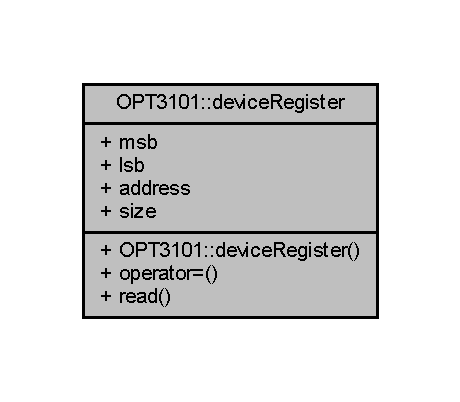
\includegraphics[width=221pt]{class_o_p_t3101_1_1device_register__coll__graph}
\end{center}
\end{figure}
\subsection*{Public Member Functions}
\begin{DoxyCompactItemize}
\item 
\mbox{\hyperlink{class_o_p_t3101_1_1device_register_a78bf911477c1d96731b716db7ea83dcb}{O\+P\+T3101\+::device\+Register}} (uint8\+\_\+t \mbox{\hyperlink{class_o_p_t3101_1_1device_register_a058d48b4c23e22739b1c65d85367a0a8}{size}})
\begin{DoxyCompactList}\small\item\em Constructor for class \mbox{\hyperlink{class_o_p_t3101_1_1device_register}{O\+P\+T3101\+::device\+Register}} Constructor allocated size to each register instance on construction. \end{DoxyCompactList}\item 
void \mbox{\hyperlink{class_o_p_t3101_1_1device_register_a0b3153b2ccbe96d37c247c605d6ba995}{operator=}} (int32\+\_\+t value)
\begin{DoxyCompactList}\small\item\em Operator overload for \textquotesingle{}=\textquotesingle{}. \end{DoxyCompactList}\item 
uint32\+\_\+t \mbox{\hyperlink{class_o_p_t3101_1_1device_register_a7092e4906eaff27555bc589eaf737493}{read}} ()
\begin{DoxyCompactList}\small\item\em Function called to read the value of register. \end{DoxyCompactList}\end{DoxyCompactItemize}
\subsection*{Public Attributes}
\begin{DoxyCompactItemize}
\item 
uint8\+\_\+t \mbox{\hyperlink{class_o_p_t3101_1_1device_register_a40f9e71d804ae858b6baed1f12b3cf83}{msb}} \mbox{[}2\mbox{]}
\begin{DoxyCompactList}\small\item\em This is the M\+SB position of this register. The register occupies the \mbox{\hyperlink{class_o_p_t3101_1_1device_register_a81d25c717489ac388db0fed33c35bedd}{O\+P\+T3101\+::device\+Register\+::address}} from \mbox{\hyperlink{class_o_p_t3101_1_1device_register_a40f9e71d804ae858b6baed1f12b3cf83}{O\+P\+T3101\+::device\+Register\+::msb}} to \mbox{\hyperlink{class_o_p_t3101_1_1device_register_a404078f369116e10b1cccfbb77c557ca}{O\+P\+T3101\+::device\+Register\+::lsb}}. \end{DoxyCompactList}\item 
uint8\+\_\+t \mbox{\hyperlink{class_o_p_t3101_1_1device_register_a404078f369116e10b1cccfbb77c557ca}{lsb}} \mbox{[}2\mbox{]}
\begin{DoxyCompactList}\small\item\em This is the L\+SB position of this register. The register occupies the \mbox{\hyperlink{class_o_p_t3101_1_1device_register_a81d25c717489ac388db0fed33c35bedd}{O\+P\+T3101\+::device\+Register\+::address}} from \mbox{\hyperlink{class_o_p_t3101_1_1device_register_a40f9e71d804ae858b6baed1f12b3cf83}{O\+P\+T3101\+::device\+Register\+::msb}} to \mbox{\hyperlink{class_o_p_t3101_1_1device_register_a404078f369116e10b1cccfbb77c557ca}{O\+P\+T3101\+::device\+Register\+::lsb}}. \end{DoxyCompactList}\item 
uint8\+\_\+t \mbox{\hyperlink{class_o_p_t3101_1_1device_register_a81d25c717489ac388db0fed33c35bedd}{address}} \mbox{[}2\mbox{]}
\begin{DoxyCompactList}\small\item\em This is the A\+D\+D\+R\+E\+SS of this register. The register occupies the \mbox{\hyperlink{class_o_p_t3101_1_1device_register_a81d25c717489ac388db0fed33c35bedd}{O\+P\+T3101\+::device\+Register\+::address}} from \mbox{\hyperlink{class_o_p_t3101_1_1device_register_a40f9e71d804ae858b6baed1f12b3cf83}{O\+P\+T3101\+::device\+Register\+::msb}} to \mbox{\hyperlink{class_o_p_t3101_1_1device_register_a404078f369116e10b1cccfbb77c557ca}{O\+P\+T3101\+::device\+Register\+::lsb}}. \end{DoxyCompactList}\item 
uint8\+\_\+t \mbox{\hyperlink{class_o_p_t3101_1_1device_register_a058d48b4c23e22739b1c65d85367a0a8}{size}}
\begin{DoxyCompactList}\small\item\em This specifies how many A\+D\+D\+R\+E\+SS does this register span across. For eg\+: There are registers which span multiple address locations in chunks. \end{DoxyCompactList}\end{DoxyCompactItemize}


\subsection{Detailed Description}
Class that contains positional information for registers in the register map. 

Class that contains positional information for a register in \mbox{\hyperlink{namespace_o_p_t3101}{O\+P\+T3101}} device. \mbox{\hyperlink{namespace_o_p_t3101}{O\+P\+T3101}} has 256 registers each 24 bits wide (\mbox{\hyperlink{class_o_p_t3101_1_1device_register_a40f9e71d804ae858b6baed1f12b3cf83}{O\+P\+T3101\+::device\+Register\+::msb}} of 23 and \mbox{\hyperlink{class_o_p_t3101_1_1device_register_a404078f369116e10b1cccfbb77c557ca}{O\+P\+T3101\+::device\+Register\+::lsb}} of 0 with \mbox{\hyperlink{class_o_p_t3101_1_1device_register_a81d25c717489ac388db0fed33c35bedd}{O\+P\+T3101\+::device\+Register\+::address}} varying from 0 to 255) Bits are groups together and are addressed with a name. Registers have names, placed at different segments of the register map. For eg\+: tmain (temperature of main temp sensor) of \mbox{\hyperlink{namespace_o_p_t3101}{O\+P\+T3101}} occupies location with address 10 from msb of 23 bits to 12 bits in other words \mbox{\hyperlink{class_o_p_t3101_1_1device_register_a81d25c717489ac388db0fed33c35bedd}{O\+P\+T3101\+::device\+Register\+::address}}=10 \mbox{\hyperlink{class_o_p_t3101_1_1device_register_a40f9e71d804ae858b6baed1f12b3cf83}{O\+P\+T3101\+::device\+Register\+::msb}}=23 \mbox{\hyperlink{class_o_p_t3101_1_1device_register_a404078f369116e10b1cccfbb77c557ca}{O\+P\+T3101\+::device\+Register\+::lsb}}=12 This class helps resolve programmers to read and write I2C to \mbox{\hyperlink{namespace_o_p_t3101}{O\+P\+T3101}} device by writing program code with higher level of abstraction with register names rather than dealing with positions of registers \mbox{\hyperlink{class_o_p_t3101_1_1device_register}{O\+P\+T3101\+::device\+Register}} class helps resolve M\+SB, L\+SB and A\+D\+D\+R\+E\+SS fields for a register by its name. ~\newline
Using this class gives user a functional name for each register making the register read and write more readable and meaningful. In case of \mbox{\hyperlink{namespace_o_p_t3101}{O\+P\+T3101}} device there are some registers which span across 2 address positions, hence the \mbox{\hyperlink{class_o_p_t3101_1_1device_register_a81d25c717489ac388db0fed33c35bedd}{O\+P\+T3101\+::device\+Register\+::address}}, \mbox{\hyperlink{class_o_p_t3101_1_1device_register_a40f9e71d804ae858b6baed1f12b3cf83}{O\+P\+T3101\+::device\+Register\+::msb}} and \mbox{\hyperlink{class_o_p_t3101_1_1device_register_a404078f369116e10b1cccfbb77c557ca}{O\+P\+T3101\+::device\+Register\+::lsb}} have 2 allocations each. In most register cases they may not end up using both the allocations. The actual usage can be found using \mbox{\hyperlink{class_o_p_t3101_1_1device_register_a058d48b4c23e22739b1c65d85367a0a8}{O\+P\+T3101\+::device\+Register\+::size}} member ~\newline
 Example of register which has more than 1 address is \mbox{\hyperlink{class_o_p_t3101_1_1registers_abdb9db1e1ff8bda71eccaea718b116d0}{O\+P\+T3101\+::registers\+::amplitude\+\_\+min\+\_\+thr}} which spans across register 0x10 from bits 23\+:16 and 0x11 from bites 23\+:16 

\subsection{Member Function Documentation}
\mbox{\Hypertarget{class_o_p_t3101_1_1device_register_a0b3153b2ccbe96d37c247c605d6ba995}\label{class_o_p_t3101_1_1device_register_a0b3153b2ccbe96d37c247c605d6ba995}} 
\index{O\+P\+T3101\+::device\+Register@{O\+P\+T3101\+::device\+Register}!operator=@{operator=}}
\index{operator=@{operator=}!O\+P\+T3101\+::device\+Register@{O\+P\+T3101\+::device\+Register}}
\subsubsection{\texorpdfstring{operator=()}{operator=()}}
{\footnotesize\ttfamily void O\+P\+T3101\+::device\+Register\+::operator= (\begin{DoxyParamCaption}\item[{int32\+\_\+t}]{value }\end{DoxyParamCaption})}



Operator overload for \textquotesingle{}=\textquotesingle{}. 

This makes calling this class simpler. dev.\+register=value will resolve the register address and value and invoke \mbox{\hyperlink{classhost_controller_a7c4126810a72333e3ebe749159a0a516}{host\+Controller\+::write\+I2C}} method With proper implementation of the \mbox{\hyperlink{classhost_controller_a7c4126810a72333e3ebe749159a0a516}{host\+Controller\+::write\+I2C}} methods the h/w would receive resolved I2C W\+R\+I\+TE commands The write operations are read modify writes to make the system robust A single call of this method could invoke up to 2 I2C R\+E\+AD and 2 I2C W\+R\+I\+TE transaction depending on the register 
\begin{DoxyParams}[1]{Parameters}
\mbox{\tt in}  & {\em value;} & value to be set to register \\
\hline
\end{DoxyParams}
\begin{DoxyReturn}{Returns}
Nothing 
\end{DoxyReturn}
\mbox{\Hypertarget{class_o_p_t3101_1_1device_register_a78bf911477c1d96731b716db7ea83dcb}\label{class_o_p_t3101_1_1device_register_a78bf911477c1d96731b716db7ea83dcb}} 
\index{O\+P\+T3101\+::device\+Register@{O\+P\+T3101\+::device\+Register}!O\+P\+T3101\+::device\+Register@{O\+P\+T3101\+::device\+Register}}
\index{O\+P\+T3101\+::device\+Register@{O\+P\+T3101\+::device\+Register}!O\+P\+T3101\+::device\+Register@{O\+P\+T3101\+::device\+Register}}
\subsubsection{\texorpdfstring{O\+P\+T3101\+::device\+Register()}{OPT3101::deviceRegister()}}
{\footnotesize\ttfamily O\+P\+T3101\+::device\+Register\+::\+O\+P\+T3101\+::device\+Register (\begin{DoxyParamCaption}\item[{uint8\+\_\+t}]{size }\end{DoxyParamCaption})}



Constructor for class \mbox{\hyperlink{class_o_p_t3101_1_1device_register}{O\+P\+T3101\+::device\+Register}} Constructor allocated size to each register instance on construction. 


\begin{DoxyParams}[1]{Parameters}
\mbox{\tt in}  & {\em size;} & size (typically 1 or 2 bytes) determines the number of segments that the register is divided in to. \\
\hline
\end{DoxyParams}
\mbox{\Hypertarget{class_o_p_t3101_1_1device_register_a7092e4906eaff27555bc589eaf737493}\label{class_o_p_t3101_1_1device_register_a7092e4906eaff27555bc589eaf737493}} 
\index{O\+P\+T3101\+::device\+Register@{O\+P\+T3101\+::device\+Register}!read@{read}}
\index{read@{read}!O\+P\+T3101\+::device\+Register@{O\+P\+T3101\+::device\+Register}}
\subsubsection{\texorpdfstring{read()}{read()}}
{\footnotesize\ttfamily uint32\+\_\+t O\+P\+T3101\+::device\+Register\+::read (\begin{DoxyParamCaption}{ }\end{DoxyParamCaption})}



Function called to read the value of register. 

This method provides an abstraction for register to be used seamlessly with code for read register operations. \mbox{\hyperlink{classhost_controller_a2bee6b3ec45fac241484f7dad943d8ed}{host\+Controller\+::read\+I2C}} method is invoked with \mbox{\hyperlink{class_o_p_t3101_1_1device_register_a81d25c717489ac388db0fed33c35bedd}{O\+P\+T3101\+::device\+Register\+::address}} fields and the resulting register value is combined as per the register positional information and reported as a uint32\+\_\+t number A single call of this method could invoke up to 2 I2C R\+E\+AD transaction depending on the register \begin{DoxyReturn}{Returns}
value; value is reading of register from \mbox{\hyperlink{namespace_o_p_t3101}{O\+P\+T3101}} device 
\end{DoxyReturn}
{\bfseries Algorithm of the method is as follows}


\begin{DoxyItemize}
\item Loops though the number of \mbox{\hyperlink{class_o_p_t3101_1_1device_register_a81d25c717489ac388db0fed33c35bedd}{O\+P\+T3101\+::device\+Register\+::address}} fields based on \mbox{\hyperlink{class_o_p_t3101_1_1device_register_a058d48b4c23e22739b1c65d85367a0a8}{O\+P\+T3101\+::device\+Register\+::size}}
\item Invokes \mbox{\hyperlink{classhost_controller_a2bee6b3ec45fac241484f7dad943d8ed}{host\+Controller\+::read\+I2\+C()}} method to get register value from h/w
\item Masks the bits for the register value to be reported based on register positional information
\item Assembles the value of the register
\item Returns the value read from the h/w for the register name specified 
\end{DoxyItemize}

\subsection{Member Data Documentation}
\mbox{\Hypertarget{class_o_p_t3101_1_1device_register_a81d25c717489ac388db0fed33c35bedd}\label{class_o_p_t3101_1_1device_register_a81d25c717489ac388db0fed33c35bedd}} 
\index{O\+P\+T3101\+::device\+Register@{O\+P\+T3101\+::device\+Register}!address@{address}}
\index{address@{address}!O\+P\+T3101\+::device\+Register@{O\+P\+T3101\+::device\+Register}}
\subsubsection{\texorpdfstring{address}{address}}
{\footnotesize\ttfamily uint8\+\_\+t O\+P\+T3101\+::device\+Register\+::address\mbox{[}2\mbox{]}}



This is the A\+D\+D\+R\+E\+SS of this register. The register occupies the \mbox{\hyperlink{class_o_p_t3101_1_1device_register_a81d25c717489ac388db0fed33c35bedd}{O\+P\+T3101\+::device\+Register\+::address}} from \mbox{\hyperlink{class_o_p_t3101_1_1device_register_a40f9e71d804ae858b6baed1f12b3cf83}{O\+P\+T3101\+::device\+Register\+::msb}} to \mbox{\hyperlink{class_o_p_t3101_1_1device_register_a404078f369116e10b1cccfbb77c557ca}{O\+P\+T3101\+::device\+Register\+::lsb}}. 

\mbox{\Hypertarget{class_o_p_t3101_1_1device_register_a404078f369116e10b1cccfbb77c557ca}\label{class_o_p_t3101_1_1device_register_a404078f369116e10b1cccfbb77c557ca}} 
\index{O\+P\+T3101\+::device\+Register@{O\+P\+T3101\+::device\+Register}!lsb@{lsb}}
\index{lsb@{lsb}!O\+P\+T3101\+::device\+Register@{O\+P\+T3101\+::device\+Register}}
\subsubsection{\texorpdfstring{lsb}{lsb}}
{\footnotesize\ttfamily uint8\+\_\+t O\+P\+T3101\+::device\+Register\+::lsb\mbox{[}2\mbox{]}}



This is the L\+SB position of this register. The register occupies the \mbox{\hyperlink{class_o_p_t3101_1_1device_register_a81d25c717489ac388db0fed33c35bedd}{O\+P\+T3101\+::device\+Register\+::address}} from \mbox{\hyperlink{class_o_p_t3101_1_1device_register_a40f9e71d804ae858b6baed1f12b3cf83}{O\+P\+T3101\+::device\+Register\+::msb}} to \mbox{\hyperlink{class_o_p_t3101_1_1device_register_a404078f369116e10b1cccfbb77c557ca}{O\+P\+T3101\+::device\+Register\+::lsb}}. 

\mbox{\Hypertarget{class_o_p_t3101_1_1device_register_a40f9e71d804ae858b6baed1f12b3cf83}\label{class_o_p_t3101_1_1device_register_a40f9e71d804ae858b6baed1f12b3cf83}} 
\index{O\+P\+T3101\+::device\+Register@{O\+P\+T3101\+::device\+Register}!msb@{msb}}
\index{msb@{msb}!O\+P\+T3101\+::device\+Register@{O\+P\+T3101\+::device\+Register}}
\subsubsection{\texorpdfstring{msb}{msb}}
{\footnotesize\ttfamily uint8\+\_\+t O\+P\+T3101\+::device\+Register\+::msb\mbox{[}2\mbox{]}}



This is the M\+SB position of this register. The register occupies the \mbox{\hyperlink{class_o_p_t3101_1_1device_register_a81d25c717489ac388db0fed33c35bedd}{O\+P\+T3101\+::device\+Register\+::address}} from \mbox{\hyperlink{class_o_p_t3101_1_1device_register_a40f9e71d804ae858b6baed1f12b3cf83}{O\+P\+T3101\+::device\+Register\+::msb}} to \mbox{\hyperlink{class_o_p_t3101_1_1device_register_a404078f369116e10b1cccfbb77c557ca}{O\+P\+T3101\+::device\+Register\+::lsb}}. 

\mbox{\Hypertarget{class_o_p_t3101_1_1device_register_a058d48b4c23e22739b1c65d85367a0a8}\label{class_o_p_t3101_1_1device_register_a058d48b4c23e22739b1c65d85367a0a8}} 
\index{O\+P\+T3101\+::device\+Register@{O\+P\+T3101\+::device\+Register}!size@{size}}
\index{size@{size}!O\+P\+T3101\+::device\+Register@{O\+P\+T3101\+::device\+Register}}
\subsubsection{\texorpdfstring{size}{size}}
{\footnotesize\ttfamily uint8\+\_\+t O\+P\+T3101\+::device\+Register\+::size}



This specifies how many A\+D\+D\+R\+E\+SS does this register span across. For eg\+: There are registers which span multiple address locations in chunks. 



The documentation for this class was generated from the following files\+:\begin{DoxyCompactItemize}
\item 
C\+:/folders/d/scripts/cpp/\+O\+P\+T3101\+S\+D\+K/\+O\+P\+T3101\+S\+D\+K/\+O\+P\+T3101\+S\+D\+K/\mbox{\hyperlink{register_8h}{register.\+h}}\item 
C\+:/folders/d/scripts/cpp/\+O\+P\+T3101\+S\+D\+K/\+O\+P\+T3101\+S\+D\+K/\+O\+P\+T3101\+S\+D\+K/\mbox{\hyperlink{register_8cpp}{register.\+cpp}}\end{DoxyCompactItemize}

\hypertarget{classenvironmental_controller}{}\section{environmental\+Controller Class Reference}
\label{classenvironmental_controller}\index{environmental\+Controller@{environmental\+Controller}}


Generic implementation for environment controller.  




{\ttfamily \#include $<$environment\+Control.\+h$>$}



Collaboration diagram for environmental\+Controller\+:\nopagebreak
\begin{figure}[H]
\begin{center}
\leavevmode
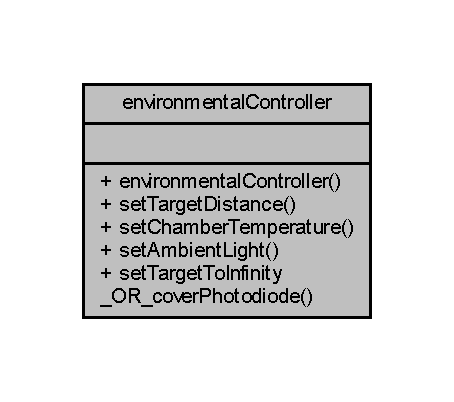
\includegraphics[width=218pt]{classenvironmental_controller__coll__graph}
\end{center}
\end{figure}
\subsection*{Public Member Functions}
\begin{DoxyCompactItemize}
\item 
\mbox{\hyperlink{classenvironmental_controller_a2dbb21c983ff11a07ef763fba57b2e76}{environmental\+Controller}} ()
\begin{DoxyCompactList}\small\item\em Constructor to initialize variables to 0. \end{DoxyCompactList}\item 
void \mbox{\hyperlink{classenvironmental_controller_a8251b7f25c6a6c5583c718bac664d05b}{set\+Target\+Distance}} (uint16\+\_\+t target\+Distance\+In\+MM)
\begin{DoxyCompactList}\small\item\em Sets target distance. \end{DoxyCompactList}\item 
void \mbox{\hyperlink{classenvironmental_controller_a3c23e944f34f2d7c0fa0b279d5fc8a3f}{set\+Chamber\+Temperature}} (int8\+\_\+t chamber\+Temperature\+InC)
\begin{DoxyCompactList}\small\item\em Sets chamber temperature. \end{DoxyCompactList}\item 
void \mbox{\hyperlink{classenvironmental_controller_adc63a8d9dbdbcef5768cf34692c6465c}{set\+Ambient\+Light}} (uint32\+\_\+t ambient\+Light\+In\+Lux)
\begin{DoxyCompactList}\small\item\em Sets ambient light condition. \end{DoxyCompactList}\item 
void \mbox{\hyperlink{classenvironmental_controller_a8a1fb44efff232844f00de18e174d4ce}{set\+Target\+To\+Infinity\+\_\+\+O\+R\+\_\+cover\+Photodiode}} ()
\begin{DoxyCompactList}\small\item\em Sets target such that the amplitude of system is very low This is a crucial step to determine \mbox{\hyperlink{class_o_p_t3101_1_1crosstalk_c}{O\+P\+T3101\+::crosstalkC}} values for the \mbox{\hyperlink{namespace_o_p_t3101}{O\+P\+T3101}} system. The environment\+Controller is expected to target in such a way that the amplitude of the system reads a low enough value that this can be ignored as crosstalk value. Either setting target to far enough position (or low enough reflectivity) or covering the photo diode would help achieve this. \end{DoxyCompactList}\end{DoxyCompactItemize}


\subsection{Detailed Description}
Generic implementation for environment controller. 

As part of O\+P\+T3101\+S\+DK there are several environment specific functions that need to be performed. Examples of such functions are setting up targets at particular distance, setting up chamber temperature. These are essential functions to perform the calibration of \mbox{\hyperlink{namespace_o_p_t3101}{O\+P\+T3101}} based system. The setting up of these environment conditions have to be done at specific steps during calibration. The template class \mbox{\hyperlink{classenvironmental_controller}{environmental\+Controller}} makes this process simple and scalable. Appropriate methods of this class are called at relevant steps in calibration. Users using this S\+DK are expected to implement these functions based on the environment setup. ~\newline
~\newline
 The names of the methods reflect the conditions for the environment. For eg\+: \mbox{\hyperlink{classenvironmental_controller_a8a1fb44efff232844f00de18e174d4ce}{environmental\+Controller\+::set\+Target\+To\+Infinity\+\_\+\+O\+R\+\_\+cover\+Photodiode}} method as the name suggest is a condition where the \mbox{\hyperlink{namespace_o_p_t3101}{O\+P\+T3101}} system needs to be pointed to infinity (far away from detectable range of system) or the photo diode needs to be covered so no light leaks directly between the transmitter(s) and photo diode. ~\newline
These implementations are very specific to the host on which the S\+DK is ported and run. ~\newline
 This abstract class provides a template with self explanatory method names which the users can override and implement their own functions. ~\newline
 

\subsection{Constructor \& Destructor Documentation}
\mbox{\Hypertarget{classenvironmental_controller_a2dbb21c983ff11a07ef763fba57b2e76}\label{classenvironmental_controller_a2dbb21c983ff11a07ef763fba57b2e76}} 
\index{environmental\+Controller@{environmental\+Controller}!environmental\+Controller@{environmental\+Controller}}
\index{environmental\+Controller@{environmental\+Controller}!environmental\+Controller@{environmental\+Controller}}
\subsubsection{\texorpdfstring{environmental\+Controller()}{environmentalController()}}
{\footnotesize\ttfamily environmental\+Controller\+::environmental\+Controller (\begin{DoxyParamCaption}{ }\end{DoxyParamCaption})}



Constructor to initialize variables to 0. 

\begin{DoxyReturn}{Returns}
Nothing 
\end{DoxyReturn}
{\bfseries Algorithm of the method is as follows}


\begin{DoxyItemize}
\item Nulls all the class members 
\end{DoxyItemize}

\subsection{Member Function Documentation}
\mbox{\Hypertarget{classenvironmental_controller_adc63a8d9dbdbcef5768cf34692c6465c}\label{classenvironmental_controller_adc63a8d9dbdbcef5768cf34692c6465c}} 
\index{environmental\+Controller@{environmental\+Controller}!set\+Ambient\+Light@{set\+Ambient\+Light}}
\index{set\+Ambient\+Light@{set\+Ambient\+Light}!environmental\+Controller@{environmental\+Controller}}
\subsubsection{\texorpdfstring{set\+Ambient\+Light()}{setAmbientLight()}}
{\footnotesize\ttfamily void environmental\+Controller\+::set\+Ambient\+Light (\begin{DoxyParamCaption}\item[{uint32\+\_\+t}]{ambient\+Light\+In\+Lux }\end{DoxyParamCaption})}



Sets ambient light condition. 


\begin{DoxyParams}[1]{Parameters}
\mbox{\tt in}  & {\em ambient\+Light\+In\+Lux;} & ambient\+Light\+In\+Lux is the intensity (in lux) of ambient light to be applied to the system to perform \mbox{\hyperlink{class_o_p_t3101_1_1phase_ambient_coff_c}{O\+P\+T3101\+::phase\+Ambient\+CoffC}} measurements \\
\hline
\end{DoxyParams}
\begin{DoxyReturn}{Returns}
Nothing 
\end{DoxyReturn}
{\bfseries Algorithm of the method is as follows} \mbox{\Hypertarget{classenvironmental_controller_a3c23e944f34f2d7c0fa0b279d5fc8a3f}\label{classenvironmental_controller_a3c23e944f34f2d7c0fa0b279d5fc8a3f}} 
\index{environmental\+Controller@{environmental\+Controller}!set\+Chamber\+Temperature@{set\+Chamber\+Temperature}}
\index{set\+Chamber\+Temperature@{set\+Chamber\+Temperature}!environmental\+Controller@{environmental\+Controller}}
\subsubsection{\texorpdfstring{set\+Chamber\+Temperature()}{setChamberTemperature()}}
{\footnotesize\ttfamily void environmental\+Controller\+::set\+Chamber\+Temperature (\begin{DoxyParamCaption}\item[{int8\+\_\+t}]{chamber\+Temperature\+InC }\end{DoxyParamCaption})}



Sets chamber temperature. 


\begin{DoxyParams}[1]{Parameters}
\mbox{\tt in}  & {\em chamber\+Temperature\+In\+C;} & chamber\+Temperature\+InC is the known temperature the chamber needs to be set to and settled. This is critical for temperature related calibration steps \\
\hline
\end{DoxyParams}
\begin{DoxyReturn}{Returns}
Nothing 
\end{DoxyReturn}
{\bfseries Algorithm of the method is as follows} \mbox{\Hypertarget{classenvironmental_controller_a8251b7f25c6a6c5583c718bac664d05b}\label{classenvironmental_controller_a8251b7f25c6a6c5583c718bac664d05b}} 
\index{environmental\+Controller@{environmental\+Controller}!set\+Target\+Distance@{set\+Target\+Distance}}
\index{set\+Target\+Distance@{set\+Target\+Distance}!environmental\+Controller@{environmental\+Controller}}
\subsubsection{\texorpdfstring{set\+Target\+Distance()}{setTargetDistance()}}
{\footnotesize\ttfamily void environmental\+Controller\+::set\+Target\+Distance (\begin{DoxyParamCaption}\item[{uint16\+\_\+t}]{target\+Distance\+In\+MM }\end{DoxyParamCaption})}



Sets target distance. 


\begin{DoxyParams}[1]{Parameters}
\mbox{\tt in}  & {\em target\+Distance\+In\+M\+M;} & target\+Distance\+In\+MM is the known distance where the target needs to be placed. This is expressed in mm \\
\hline
\end{DoxyParams}
\begin{DoxyReturn}{Returns}
Nothing 
\end{DoxyReturn}
{\bfseries Algorithm of the method is as follows}


\begin{DoxyItemize}
\item User implemented function to set the target distance 
\end{DoxyItemize}\mbox{\Hypertarget{classenvironmental_controller_a8a1fb44efff232844f00de18e174d4ce}\label{classenvironmental_controller_a8a1fb44efff232844f00de18e174d4ce}} 
\index{environmental\+Controller@{environmental\+Controller}!set\+Target\+To\+Infinity\+\_\+\+O\+R\+\_\+cover\+Photodiode@{set\+Target\+To\+Infinity\+\_\+\+O\+R\+\_\+cover\+Photodiode}}
\index{set\+Target\+To\+Infinity\+\_\+\+O\+R\+\_\+cover\+Photodiode@{set\+Target\+To\+Infinity\+\_\+\+O\+R\+\_\+cover\+Photodiode}!environmental\+Controller@{environmental\+Controller}}
\subsubsection{\texorpdfstring{set\+Target\+To\+Infinity\+\_\+\+O\+R\+\_\+cover\+Photodiode()}{setTargetToInfinity\_OR\_coverPhotodiode()}}
{\footnotesize\ttfamily void environmental\+Controller\+::set\+Target\+To\+Infinity\+\_\+\+O\+R\+\_\+cover\+Photodiode (\begin{DoxyParamCaption}{ }\end{DoxyParamCaption})}



Sets target such that the amplitude of system is very low This is a crucial step to determine \mbox{\hyperlink{class_o_p_t3101_1_1crosstalk_c}{O\+P\+T3101\+::crosstalkC}} values for the \mbox{\hyperlink{namespace_o_p_t3101}{O\+P\+T3101}} system. The environment\+Controller is expected to target in such a way that the amplitude of the system reads a low enough value that this can be ignored as crosstalk value. Either setting target to far enough position (or low enough reflectivity) or covering the photo diode would help achieve this. 

\begin{DoxyReturn}{Returns}
Nothing 
\end{DoxyReturn}
{\bfseries Algorithm of the method is as follows}
\begin{DoxyItemize}
\item This is an empty function to convey the measurement setup required.
\item With a cover glass in place, the system is expected to be pointed towards a target with very low reflectivity far beyond the range of the system
\item It is also acceptable to cover the photo diode alone with an optically isolating light blocker. 
\end{DoxyItemize}

The documentation for this class was generated from the following files\+:\begin{DoxyCompactItemize}
\item 
C\+:/folders/d/scripts/cpp/\+O\+P\+T3101\+S\+D\+K/\+O\+P\+T3101\+S\+D\+K/\+O\+P\+T3101\+S\+D\+K/\mbox{\hyperlink{environment_control_8h}{environment\+Control.\+h}}\item 
C\+:/folders/d/scripts/cpp/\+O\+P\+T3101\+S\+D\+K/\+O\+P\+T3101\+S\+D\+K/\+O\+P\+T3101\+S\+D\+K/\mbox{\hyperlink{environment_control_8cpp}{environment\+Control.\+cpp}}\end{DoxyCompactItemize}

\hypertarget{class_o_p_t3101_1_1frame_data}{}\section{O\+P\+T3101\+:\+:frame\+Data Class Reference}
\label{class_o_p_t3101_1_1frame_data}\index{O\+P\+T3101\+::frame\+Data@{O\+P\+T3101\+::frame\+Data}}


Class the data output from \mbox{\hyperlink{namespace_o_p_t3101}{O\+P\+T3101}} device.  




{\ttfamily \#include $<$O\+P\+T3101frame\+Data.\+h$>$}



Collaboration diagram for O\+P\+T3101\+:\+:frame\+Data\+:\nopagebreak
\begin{figure}[H]
\begin{center}
\leavevmode
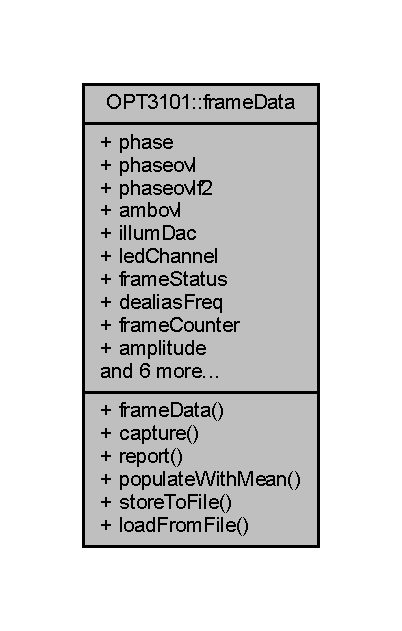
\includegraphics[width=193pt]{class_o_p_t3101_1_1frame_data__coll__graph}
\end{center}
\end{figure}
\subsection*{Public Member Functions}
\begin{DoxyCompactItemize}
\item 
\mbox{\hyperlink{class_o_p_t3101_1_1frame_data_a75a43907483d7d3b2db46cfb10bfd568}{frame\+Data}} ()
\begin{DoxyCompactList}\small\item\em initializes the members to 0 \end{DoxyCompactList}\item 
void \mbox{\hyperlink{class_o_p_t3101_1_1frame_data_a0ea9d9f3fc2d25e28e77855f4db8e2a6}{capture}} (\mbox{\hyperlink{classhost_controller}{host\+Controller}} $\ast$\mbox{\hyperlink{host_controller_8h_a47f8cbf152e48aa4fdb624be57a9a856}{host}}, \mbox{\hyperlink{class_o_p_t3101_1_1device}{device}} $\ast$dev, bool read\+T\+Illulm=true)
\begin{DoxyCompactList}\small\item\em captures measurement data from the device This method invokes I2C transactions to capture data from the \mbox{\hyperlink{namespace_o_p_t3101}{O\+P\+T3101}} device registers 0x08, 0x09 and 0x0A. Extracts and assigns members their respective values based on their positions in the registers. \end{DoxyCompactList}\item 
void \mbox{\hyperlink{class_o_p_t3101_1_1frame_data_ad20da1bc47279244384f59c2f3b33d61}{report}} ()
\begin{DoxyCompactList}\small\item\em reports members of the instance Print the members of the class instance on screen \end{DoxyCompactList}\item 
void \mbox{\hyperlink{class_o_p_t3101_1_1frame_data_a2fe90347589e7c97cc9fade2c68fa10f}{populate\+With\+Mean}} (\mbox{\hyperlink{class_o_p_t3101_1_1frame_data}{frame\+Data}} $\ast$input\+Data, uint16\+\_\+t n\+Frames)
\begin{DoxyCompactList}\small\item\em calculates mean and assigns to self Given a set on input \mbox{\hyperlink{class_o_p_t3101_1_1frame_data}{O\+P\+T3101\+::frame\+Data}} the method calculates the mean frame and assigns to self \end{DoxyCompactList}\item 
void \mbox{\hyperlink{class_o_p_t3101_1_1frame_data_a8ece44f845216c8d0cae378932c854e6}{store\+To\+File}} (char $\ast$file\+Name)
\begin{DoxyCompactList}\small\item\em saves phase temp coff values to file This methods saves the phase temp coff values to a non-\/volatile memory. Storage/\+Restoration to/from non-\/volatile memory is important for factory calibration \end{DoxyCompactList}\item 
void \mbox{\hyperlink{class_o_p_t3101_1_1frame_data_aca9b96c6a896ee6caab380e05ae45064}{load\+From\+File}} (char $\ast$file\+Name)
\begin{DoxyCompactList}\small\item\em load phase temp coff values from file This methods loads the phase temp coff values to a non-\/volatile memory. Storage/\+Restoration to/from non-\/volatile memory is important for factory calibration \end{DoxyCompactList}\end{DoxyCompactItemize}
\subsection*{Public Attributes}
\begin{DoxyCompactItemize}
\item 
uint32\+\_\+t \mbox{\hyperlink{class_o_p_t3101_1_1frame_data_af8661d11405953dc378ad4d7cb0f2db6}{phase}}
\begin{DoxyCompactList}\small\item\em phase value measured by the A\+FE. Actually 16 bit unsigned value upscaled to 17 bits with 1 bit of \mbox{\hyperlink{class_o_p_t3101_1_1frame_data_ad1c9f22f2b5a22ce7977334a5ae8ef54}{frame\+Data\+::phaseovl}} flag added to the M\+SB. Same as \mbox{\hyperlink{class_o_p_t3101_1_1registers_a0b410cb503df506724a4b6a1da49ce1e}{O\+P\+T3101\+::registers\+::phase\+\_\+out}} \end{DoxyCompactList}\item 
bool \mbox{\hyperlink{class_o_p_t3101_1_1frame_data_ad1c9f22f2b5a22ce7977334a5ae8ef54}{phaseovl}}
\begin{DoxyCompactList}\small\item\em phase overload flag, specifying if phase value detected exceeds 16 bits. (greater than 65535). \mbox{\hyperlink{class_o_p_t3101_1_1registers}{O\+P\+T3101\+::registers}}\+:\+:.phase\+\_\+overflow \end{DoxyCompactList}\item 
bool \mbox{\hyperlink{class_o_p_t3101_1_1frame_data_afa41c051623d5431aa7c9d27bdb32f6c}{phaseovlf2}}
\begin{DoxyCompactList}\small\item\em phase overload flag for frequency 2, specifying if phase value detected exceeds 16 bits. (greater than 65535). Same as \mbox{\hyperlink{class_o_p_t3101_1_1registers_a63560e719cf9970bc83879a353b2dc9f}{O\+P\+T3101\+::registers\+::phase\+\_\+overflow\+\_\+f2}} \end{DoxyCompactList}\item 
bool \mbox{\hyperlink{class_o_p_t3101_1_1frame_data_ac3c39e0f87987858d5db6291c6b6d4fa}{ambovl}}
\begin{DoxyCompactList}\small\item\em ambient over load flag which flags if the A\+FE is saturated due to very high ambient condition. Same as \mbox{\hyperlink{class_o_p_t3101_1_1registers_a5ba6f5ef459327f64179b6d405dbd101}{O\+P\+T3101\+::registers\+::amb\+\_\+ovl\+\_\+flag}} \end{DoxyCompactList}\item 
bool \mbox{\hyperlink{class_o_p_t3101_1_1frame_data_ada9279b0ee78ff855e95d1e34462cbaf}{illum\+Dac}}
\begin{DoxyCompactList}\small\item\em flag that specifies which of the auto-\/hdr register config from where the measurement is made. Same as \mbox{\hyperlink{class_o_p_t3101_1_1registers_a78e8bc6ad4a84c7d19974ba6c58e329e}{O\+P\+T3101\+::registers\+::hdr\+\_\+mode}} \end{DoxyCompactList}\item 
uint8\+\_\+t \mbox{\hyperlink{class_o_p_t3101_1_1frame_data_adac0d179c89ba3b8b10b0785c80d37fa}{led\+Channel}}
\begin{DoxyCompactList}\small\item\em value that specifies from which channel the measurement is made. Same as \mbox{\hyperlink{class_o_p_t3101_1_1registers_a53518f25f00a5926fda5f0d37ad82fcb}{O\+P\+T3101\+::registers\+::tx\+\_\+channel}} \end{DoxyCompactList}\item 
bool \mbox{\hyperlink{class_o_p_t3101_1_1frame_data_ad291a49c4cfe78bb8de52749d9c0d318}{frame\+Status}}
\begin{DoxyCompactList}\small\item\em flag that specifies if the measurement is a valid data. Same as \mbox{\hyperlink{class_o_p_t3101_1_1registers_ab8c08b83252a06c3c59b4b33b4b1a8ba}{O\+P\+T3101\+::registers\+::frame\+\_\+status}} \end{DoxyCompactList}\item 
bool \mbox{\hyperlink{class_o_p_t3101_1_1frame_data_a7f4b242739da2cabd965a01d1362c38e}{dealias\+Freq}}
\begin{DoxyCompactList}\small\item\em flag that specifies if the measurement is done with fundamental frequency of de-\/alias frequency. Same as \mbox{\hyperlink{class_o_p_t3101_1_1registers_ad0a150fb8c5e1efeae026e76f2bdbc1f}{O\+P\+T3101\+::registers\+::mod\+\_\+freq}} \end{DoxyCompactList}\item 
uint8\+\_\+t \mbox{\hyperlink{class_o_p_t3101_1_1frame_data_a571ec2f70947b37d3597d5ee623367d4}{frame\+Counter}}
\begin{DoxyCompactList}\small\item\em Frame counter which counts every data ready. Same as combination of O\+P\+T3101\+::register\+::frame\+\_\+count0 , \mbox{\hyperlink{class_o_p_t3101_1_1registers_a736858f4b79f2dd5444fc1938148d438}{O\+P\+T3101\+::registers\+::frame\+\_\+count1}} and \mbox{\hyperlink{class_o_p_t3101_1_1registers_a1247368fca5573a9ab4b69d541c53a57}{O\+P\+T3101\+::registers\+::frame\+\_\+count2}}. \end{DoxyCompactList}\item 
uint16\+\_\+t \mbox{\hyperlink{class_o_p_t3101_1_1frame_data_a16b903f0cea13dc66d751beab7271a18}{amplitude}}
\begin{DoxyCompactList}\small\item\em amplitude value measured by A\+FE. 15 bit representation of the signal. Same as \mbox{\hyperlink{class_o_p_t3101_1_1registers_a09663efd977de72bdf7820e0a8f92390}{O\+P\+T3101\+::registers\+::amp\+\_\+out}} \end{DoxyCompactList}\item 
bool \mbox{\hyperlink{class_o_p_t3101_1_1frame_data_a5fde4a7c755e99367d2fc79feb51cf1b}{sigovl}}
\begin{DoxyCompactList}\small\item\em flag that specifies if the A\+FE is saturated due to signal. Same as \mbox{\hyperlink{class_o_p_t3101_1_1registers_ad767a496a0cad5741d575a54a095add3}{O\+P\+T3101\+::registers\+::sig\+\_\+ovl\+\_\+flag}} \end{DoxyCompactList}\item 
uint8\+\_\+t \mbox{\hyperlink{class_o_p_t3101_1_1frame_data_ab29ea3b01c14d5fab239039a61ca4594}{dealias\+Bin}}
\begin{DoxyCompactList}\small\item\em value that specifies the de-\/aliased bin number. Same as \mbox{\hyperlink{class_o_p_t3101_1_1registers_a1faab11698859e9d42e148c1d8cd5d1e}{O\+P\+T3101\+::registers\+::dealias\+\_\+bin}} \end{DoxyCompactList}\item 
uint16\+\_\+t \mbox{\hyperlink{class_o_p_t3101_1_1frame_data_a39ebf8bd06141bef6986e49013d03c35}{ambient}}
\begin{DoxyCompactList}\small\item\em value specifies the ambient light measured by the ambient cancellation block. Same as \mbox{\hyperlink{class_o_p_t3101_1_1registers_ae6b7c86e96cbfb1efe3263caed9de137}{O\+P\+T3101\+::registers\+::amb\+\_\+data}} \end{DoxyCompactList}\item 
uint16\+\_\+t \mbox{\hyperlink{class_o_p_t3101_1_1frame_data_a537975687785cc0fb002dc70384af7ab}{temp}}
\begin{DoxyCompactList}\small\item\em value of internal temp sensor read from register 0x0A. Same as \mbox{\hyperlink{class_o_p_t3101_1_1registers_a3dfd8d81d4cb04d274007deb7c6122fc}{O\+P\+T3101\+::registers\+::tmain}} . This is updated every data ready. \end{DoxyCompactList}\item 
uint16\+\_\+t \mbox{\hyperlink{class_o_p_t3101_1_1frame_data_ae75ca7e9fa494b4d711eb070d5cab45b}{tmain}}
\begin{DoxyCompactList}\small\item\em value of internal temp sensor read from register \mbox{\hyperlink{class_o_p_t3101_1_1registers_a3dfd8d81d4cb04d274007deb7c6122fc}{O\+P\+T3101\+::registers\+::tmain}} \end{DoxyCompactList}\item 
uint16\+\_\+t \mbox{\hyperlink{class_o_p_t3101_1_1frame_data_aeb1934ab0ac8d1f846cf166ef26ceb75}{tillum}}
\begin{DoxyCompactList}\small\item\em value of external temp sensor read using the I2C Master. Same as \mbox{\hyperlink{class_o_p_t3101_1_1registers_a8a097a41ecdf2b98226c4a3a92121c12}{O\+P\+T3101\+::registers\+::tillum}} \end{DoxyCompactList}\end{DoxyCompactItemize}
\subsection*{Friends}
\begin{DoxyCompactItemize}
\item 
std\+::ostream \& \mbox{\hyperlink{class_o_p_t3101_1_1frame_data_a01b42d736d5c28f4061d11fea440e237}{operator$<$$<$}} (std\+::ostream \&os, const \mbox{\hyperlink{class_o_p_t3101_1_1frame_data}{frame\+Data}} $\ast$data)
\begin{DoxyCompactList}\small\item\em Operator overload to store class contents to a file Casts all the class members for file storage. \end{DoxyCompactList}\item 
std\+::istream \& \mbox{\hyperlink{class_o_p_t3101_1_1frame_data_a1e4d3c11fc552ec13eb14e06164bfad6}{operator$>$$>$}} (std\+::istream \&is, \mbox{\hyperlink{class_o_p_t3101_1_1frame_data}{frame\+Data}} $\ast$data)
\begin{DoxyCompactList}\small\item\em Operator overload to load class contents to from a file Retreives all the class members from a stored file. \end{DoxyCompactList}\end{DoxyCompactItemize}


\subsection{Detailed Description}
Class the data output from \mbox{\hyperlink{namespace_o_p_t3101}{O\+P\+T3101}} device. 

This is a class that holds output data from \mbox{\hyperlink{namespace_o_p_t3101}{O\+P\+T3101}} A\+FE. Measurements by A\+FE \mbox{\hyperlink{namespace_o_p_t3101}{O\+P\+T3101}} device are stores in registers with address 0x08, x09 \& 0x0A. Difference sections of these registers hold different measurements like \mbox{\hyperlink{class_o_p_t3101_1_1frame_data_af8661d11405953dc378ad4d7cb0f2db6}{O\+P\+T3101\+::frame\+Data\+::phase}}, \mbox{\hyperlink{class_o_p_t3101_1_1frame_data_a16b903f0cea13dc66d751beab7271a18}{O\+P\+T3101\+::frame\+Data\+::amplitude}} ~\newline
 This class provides an abstraction where the registers are read, relevant portions of the registers are extracted and assigned to members with meaningful names. This provides a functional abstraction to the user. 

\subsection{Constructor \& Destructor Documentation}
\mbox{\Hypertarget{class_o_p_t3101_1_1frame_data_a75a43907483d7d3b2db46cfb10bfd568}\label{class_o_p_t3101_1_1frame_data_a75a43907483d7d3b2db46cfb10bfd568}} 
\index{O\+P\+T3101\+::frame\+Data@{O\+P\+T3101\+::frame\+Data}!frame\+Data@{frame\+Data}}
\index{frame\+Data@{frame\+Data}!O\+P\+T3101\+::frame\+Data@{O\+P\+T3101\+::frame\+Data}}
\subsubsection{\texorpdfstring{frame\+Data()}{frameData()}}
{\footnotesize\ttfamily O\+P\+T3101\+::frame\+Data\+::frame\+Data (\begin{DoxyParamCaption}{ }\end{DoxyParamCaption})}



initializes the members to 0 

\begin{DoxyReturn}{Returns}
Nothing; 
\end{DoxyReturn}
{\bfseries Algorithm of the method is as follows}


\begin{DoxyItemize}
\item Initializes all members to 0 
\end{DoxyItemize}

\subsection{Member Function Documentation}
\mbox{\Hypertarget{class_o_p_t3101_1_1frame_data_a0ea9d9f3fc2d25e28e77855f4db8e2a6}\label{class_o_p_t3101_1_1frame_data_a0ea9d9f3fc2d25e28e77855f4db8e2a6}} 
\index{O\+P\+T3101\+::frame\+Data@{O\+P\+T3101\+::frame\+Data}!capture@{capture}}
\index{capture@{capture}!O\+P\+T3101\+::frame\+Data@{O\+P\+T3101\+::frame\+Data}}
\subsubsection{\texorpdfstring{capture()}{capture()}}
{\footnotesize\ttfamily void O\+P\+T3101\+::frame\+Data\+::capture (\begin{DoxyParamCaption}\item[{\mbox{\hyperlink{classhost_controller}{host\+Controller}} $\ast$}]{host,  }\item[{\mbox{\hyperlink{class_o_p_t3101_1_1device}{O\+P\+T3101\+::device}} $\ast$}]{dev,  }\item[{bool}]{read\+T\+Illulm = {\ttfamily true} }\end{DoxyParamCaption})}



captures measurement data from the device This method invokes I2C transactions to capture data from the \mbox{\hyperlink{namespace_o_p_t3101}{O\+P\+T3101}} device registers 0x08, 0x09 and 0x0A. Extracts and assigns members their respective values based on their positions in the registers. 


\begin{DoxyParams}[1]{Parameters}
\mbox{\tt in}  & {\em host;} & Pointer to the class \mbox{\hyperlink{classhost_controller}{host\+Controller}} used to directly invoke I2C transactions bypassing \mbox{\hyperlink{class_o_p_t3101_1_1registers}{O\+P\+T3101\+::registers}} or \mbox{\hyperlink{class_o_p_t3101_1_1device}{O\+P\+T3101\+::device}} class \\
\hline
\mbox{\tt in}  & {\em dev;} & Pointer to the class \mbox{\hyperlink{class_o_p_t3101_1_1device}{O\+P\+T3101\+::device}} used to read register(s) from device \\
\hline
\mbox{\tt in}  & {\em read\+T\+Illulm;} & Flag which specifies if \mbox{\hyperlink{class_o_p_t3101_1_1registers_a8a097a41ecdf2b98226c4a3a92121c12}{O\+P\+T3101\+::registers\+::tillum}} value needs to be read or not \\
\hline
\end{DoxyParams}
\begin{DoxyReturn}{Returns}
Nothing; 
\end{DoxyReturn}
{\bfseries Algorithm of the method is as follows}


\begin{DoxyItemize}
\item Sleep host for a specified time depending on device configuration to \mbox{\hyperlink{namespace_o_p_t3101}{O\+P\+T3101}} A\+FE can update measurements to the registers.
\item Performs a direct read of I2C registers 0x08 0x09 and 0x0A directly though \mbox{\hyperlink{classhost_controller_a2bee6b3ec45fac241484f7dad943d8ed}{host\+Controller\+::read\+I2C}} method ~\newline
~\newline

\item Maps the I2C read values to the class members like \mbox{\hyperlink{class_o_p_t3101_1_1frame_data_af8661d11405953dc378ad4d7cb0f2db6}{O\+P\+T3101\+::frame\+Data\+::phase}}, \mbox{\hyperlink{class_o_p_t3101_1_1frame_data_a16b903f0cea13dc66d751beab7271a18}{O\+P\+T3101\+::frame\+Data\+::amplitude}} etc ~\newline

\item Based on read\+Illum flag reads the \mbox{\hyperlink{class_o_p_t3101_1_1registers_a8a097a41ecdf2b98226c4a3a92121c12}{O\+P\+T3101\+::registers\+::tillum}} and assigns to \mbox{\hyperlink{class_o_p_t3101_1_1frame_data_aeb1934ab0ac8d1f846cf166ef26ceb75}{O\+P\+T3101\+::frame\+Data\+::tillum}} 
\end{DoxyItemize}\mbox{\Hypertarget{class_o_p_t3101_1_1frame_data_aca9b96c6a896ee6caab380e05ae45064}\label{class_o_p_t3101_1_1frame_data_aca9b96c6a896ee6caab380e05ae45064}} 
\index{O\+P\+T3101\+::frame\+Data@{O\+P\+T3101\+::frame\+Data}!load\+From\+File@{load\+From\+File}}
\index{load\+From\+File@{load\+From\+File}!O\+P\+T3101\+::frame\+Data@{O\+P\+T3101\+::frame\+Data}}
\subsubsection{\texorpdfstring{load\+From\+File()}{loadFromFile()}}
{\footnotesize\ttfamily void O\+P\+T3101\+::frame\+Data\+::load\+From\+File (\begin{DoxyParamCaption}\item[{char $\ast$}]{file\+Name }\end{DoxyParamCaption})}



load phase temp coff values from file This methods loads the phase temp coff values to a non-\/volatile memory. Storage/\+Restoration to/from non-\/volatile memory is important for factory calibration 


\begin{DoxyParams}[1]{Parameters}
\mbox{\tt in}  & {\em file\+Name;} & Path and name of the file from where to load \\
\hline
\end{DoxyParams}
\begin{DoxyReturn}{Returns}
Nothing; 
\end{DoxyReturn}
{\bfseries Algorithm of the method is as follows}


\begin{DoxyItemize}
\item User needs to implement file load/restore based on host. 
\end{DoxyItemize}\mbox{\Hypertarget{class_o_p_t3101_1_1frame_data_a2fe90347589e7c97cc9fade2c68fa10f}\label{class_o_p_t3101_1_1frame_data_a2fe90347589e7c97cc9fade2c68fa10f}} 
\index{O\+P\+T3101\+::frame\+Data@{O\+P\+T3101\+::frame\+Data}!populate\+With\+Mean@{populate\+With\+Mean}}
\index{populate\+With\+Mean@{populate\+With\+Mean}!O\+P\+T3101\+::frame\+Data@{O\+P\+T3101\+::frame\+Data}}
\subsubsection{\texorpdfstring{populate\+With\+Mean()}{populateWithMean()}}
{\footnotesize\ttfamily void O\+P\+T3101\+::frame\+Data\+::populate\+With\+Mean (\begin{DoxyParamCaption}\item[{\mbox{\hyperlink{class_o_p_t3101_1_1frame_data}{O\+P\+T3101\+::frame\+Data}} $\ast$}]{input\+Data,  }\item[{uint16\+\_\+t}]{n\+Frames }\end{DoxyParamCaption})}



calculates mean and assigns to self Given a set on input \mbox{\hyperlink{class_o_p_t3101_1_1frame_data}{O\+P\+T3101\+::frame\+Data}} the method calculates the mean frame and assigns to self 


\begin{DoxyParams}[1]{Parameters}
\mbox{\tt in}  & {\em input\+Data;} & Pointer to the class \mbox{\hyperlink{class_o_p_t3101_1_1frame_data}{O\+P\+T3101\+::frame\+Data}} instance with multiple frame data \\
\hline
\mbox{\tt in}  & {\em n\+Frames;} & Number of measurements to step though in the input\+Data to calculate mean \\
\hline
\end{DoxyParams}
\begin{DoxyReturn}{Returns}
Nothing; 
\end{DoxyReturn}
{\bfseries Algorithm of the method is as follows}


\begin{DoxyItemize}
\item Sets n\+Frames to 1 when n\+Frames is 0
\item Finds the smallest 2$^\wedge$N number higher than the n\+Frames provided in the argument of this method
\item Accumulates and measures mean for all the input class instance members and assigns them to the method\textquotesingle{}s class members ~\newline

\item {\bfseries Warning\+:} When n\+Frames is a non 2$^\wedge$N number the mean results are expected to be lower than actual measurements 
\end{DoxyItemize}\mbox{\Hypertarget{class_o_p_t3101_1_1frame_data_ad20da1bc47279244384f59c2f3b33d61}\label{class_o_p_t3101_1_1frame_data_ad20da1bc47279244384f59c2f3b33d61}} 
\index{O\+P\+T3101\+::frame\+Data@{O\+P\+T3101\+::frame\+Data}!report@{report}}
\index{report@{report}!O\+P\+T3101\+::frame\+Data@{O\+P\+T3101\+::frame\+Data}}
\subsubsection{\texorpdfstring{report()}{report()}}
{\footnotesize\ttfamily void O\+P\+T3101\+::frame\+Data\+::report (\begin{DoxyParamCaption}{ }\end{DoxyParamCaption})}



reports members of the instance Print the members of the class instance on screen 

\begin{DoxyReturn}{Returns}
Nothing; 
\end{DoxyReturn}
{\bfseries Algorithm of the method is as follows}


\begin{DoxyItemize}
\item Prints all the members and values of members on screen. ~\newline

\item Prints all the members and values of members on screen. 
\end{DoxyItemize}\mbox{\Hypertarget{class_o_p_t3101_1_1frame_data_a8ece44f845216c8d0cae378932c854e6}\label{class_o_p_t3101_1_1frame_data_a8ece44f845216c8d0cae378932c854e6}} 
\index{O\+P\+T3101\+::frame\+Data@{O\+P\+T3101\+::frame\+Data}!store\+To\+File@{store\+To\+File}}
\index{store\+To\+File@{store\+To\+File}!O\+P\+T3101\+::frame\+Data@{O\+P\+T3101\+::frame\+Data}}
\subsubsection{\texorpdfstring{store\+To\+File()}{storeToFile()}}
{\footnotesize\ttfamily void O\+P\+T3101\+::frame\+Data\+::store\+To\+File (\begin{DoxyParamCaption}\item[{char $\ast$}]{file\+Name }\end{DoxyParamCaption})}



saves phase temp coff values to file This methods saves the phase temp coff values to a non-\/volatile memory. Storage/\+Restoration to/from non-\/volatile memory is important for factory calibration 


\begin{DoxyParams}[1]{Parameters}
\mbox{\tt in}  & {\em file\+Name;} & Path and name of the file to store \\
\hline
\end{DoxyParams}
\begin{DoxyReturn}{Returns}
Nothing; 
\end{DoxyReturn}
{\bfseries Algorithm of the method is as follows}


\begin{DoxyItemize}
\item User needs to implement file storage based on host. 
\end{DoxyItemize}

\subsection{Friends And Related Function Documentation}
\mbox{\Hypertarget{class_o_p_t3101_1_1frame_data_a01b42d736d5c28f4061d11fea440e237}\label{class_o_p_t3101_1_1frame_data_a01b42d736d5c28f4061d11fea440e237}} 
\index{O\+P\+T3101\+::frame\+Data@{O\+P\+T3101\+::frame\+Data}!operator$<$$<$@{operator$<$$<$}}
\index{operator$<$$<$@{operator$<$$<$}!O\+P\+T3101\+::frame\+Data@{O\+P\+T3101\+::frame\+Data}}
\subsubsection{\texorpdfstring{operator$<$$<$}{operator<<}}
{\footnotesize\ttfamily std\+::ostream\& operator$<$$<$ (\begin{DoxyParamCaption}\item[{std\+::ostream \&}]{os,  }\item[{const \mbox{\hyperlink{class_o_p_t3101_1_1frame_data}{frame\+Data}} $\ast$}]{data }\end{DoxyParamCaption})\hspace{0.3cm}{\ttfamily [friend]}}



Operator overload to store class contents to a file Casts all the class members for file storage. 


\begin{DoxyParams}[1]{Parameters}
\mbox{\tt out}  & {\em os;} & os is data stream to serialize data \\
\hline
\mbox{\tt in}  & {\em data;} & data is pointer to the class to be serlialized and stored \\
\hline
\end{DoxyParams}
\begin{DoxyReturn}{Returns}
std\+::ostream; Serialized std\+::ostream to be written to a file 
\end{DoxyReturn}
\mbox{\Hypertarget{class_o_p_t3101_1_1frame_data_a1e4d3c11fc552ec13eb14e06164bfad6}\label{class_o_p_t3101_1_1frame_data_a1e4d3c11fc552ec13eb14e06164bfad6}} 
\index{O\+P\+T3101\+::frame\+Data@{O\+P\+T3101\+::frame\+Data}!operator$>$$>$@{operator$>$$>$}}
\index{operator$>$$>$@{operator$>$$>$}!O\+P\+T3101\+::frame\+Data@{O\+P\+T3101\+::frame\+Data}}
\subsubsection{\texorpdfstring{operator$>$$>$}{operator>>}}
{\footnotesize\ttfamily std\+::istream\& operator$>$$>$ (\begin{DoxyParamCaption}\item[{std\+::istream \&}]{is,  }\item[{\mbox{\hyperlink{class_o_p_t3101_1_1frame_data}{frame\+Data}} $\ast$}]{data }\end{DoxyParamCaption})\hspace{0.3cm}{\ttfamily [friend]}}



Operator overload to load class contents to from a file Retreives all the class members from a stored file. 


\begin{DoxyParams}[1]{Parameters}
\mbox{\tt in}  & {\em is;} & is input stream from where the data is loaded \\
\hline
\mbox{\tt out}  & {\em data;} & data is pointer to the class to be restored \\
\hline
\end{DoxyParams}
\begin{DoxyReturn}{Returns}
std\+::istream; Serialized Input stream loaded from file 
\end{DoxyReturn}


\subsection{Member Data Documentation}
\mbox{\Hypertarget{class_o_p_t3101_1_1frame_data_a39ebf8bd06141bef6986e49013d03c35}\label{class_o_p_t3101_1_1frame_data_a39ebf8bd06141bef6986e49013d03c35}} 
\index{O\+P\+T3101\+::frame\+Data@{O\+P\+T3101\+::frame\+Data}!ambient@{ambient}}
\index{ambient@{ambient}!O\+P\+T3101\+::frame\+Data@{O\+P\+T3101\+::frame\+Data}}
\subsubsection{\texorpdfstring{ambient}{ambient}}
{\footnotesize\ttfamily uint16\+\_\+t O\+P\+T3101\+::frame\+Data\+::ambient}



value specifies the ambient light measured by the ambient cancellation block. Same as \mbox{\hyperlink{class_o_p_t3101_1_1registers_ae6b7c86e96cbfb1efe3263caed9de137}{O\+P\+T3101\+::registers\+::amb\+\_\+data}} 

\mbox{\Hypertarget{class_o_p_t3101_1_1frame_data_ac3c39e0f87987858d5db6291c6b6d4fa}\label{class_o_p_t3101_1_1frame_data_ac3c39e0f87987858d5db6291c6b6d4fa}} 
\index{O\+P\+T3101\+::frame\+Data@{O\+P\+T3101\+::frame\+Data}!ambovl@{ambovl}}
\index{ambovl@{ambovl}!O\+P\+T3101\+::frame\+Data@{O\+P\+T3101\+::frame\+Data}}
\subsubsection{\texorpdfstring{ambovl}{ambovl}}
{\footnotesize\ttfamily bool O\+P\+T3101\+::frame\+Data\+::ambovl}



ambient over load flag which flags if the A\+FE is saturated due to very high ambient condition. Same as \mbox{\hyperlink{class_o_p_t3101_1_1registers_a5ba6f5ef459327f64179b6d405dbd101}{O\+P\+T3101\+::registers\+::amb\+\_\+ovl\+\_\+flag}} 

\mbox{\Hypertarget{class_o_p_t3101_1_1frame_data_a16b903f0cea13dc66d751beab7271a18}\label{class_o_p_t3101_1_1frame_data_a16b903f0cea13dc66d751beab7271a18}} 
\index{O\+P\+T3101\+::frame\+Data@{O\+P\+T3101\+::frame\+Data}!amplitude@{amplitude}}
\index{amplitude@{amplitude}!O\+P\+T3101\+::frame\+Data@{O\+P\+T3101\+::frame\+Data}}
\subsubsection{\texorpdfstring{amplitude}{amplitude}}
{\footnotesize\ttfamily uint16\+\_\+t O\+P\+T3101\+::frame\+Data\+::amplitude}



amplitude value measured by A\+FE. 15 bit representation of the signal. Same as \mbox{\hyperlink{class_o_p_t3101_1_1registers_a09663efd977de72bdf7820e0a8f92390}{O\+P\+T3101\+::registers\+::amp\+\_\+out}} 

\mbox{\Hypertarget{class_o_p_t3101_1_1frame_data_ab29ea3b01c14d5fab239039a61ca4594}\label{class_o_p_t3101_1_1frame_data_ab29ea3b01c14d5fab239039a61ca4594}} 
\index{O\+P\+T3101\+::frame\+Data@{O\+P\+T3101\+::frame\+Data}!dealias\+Bin@{dealias\+Bin}}
\index{dealias\+Bin@{dealias\+Bin}!O\+P\+T3101\+::frame\+Data@{O\+P\+T3101\+::frame\+Data}}
\subsubsection{\texorpdfstring{dealias\+Bin}{dealiasBin}}
{\footnotesize\ttfamily uint8\+\_\+t O\+P\+T3101\+::frame\+Data\+::dealias\+Bin}



value that specifies the de-\/aliased bin number. Same as \mbox{\hyperlink{class_o_p_t3101_1_1registers_a1faab11698859e9d42e148c1d8cd5d1e}{O\+P\+T3101\+::registers\+::dealias\+\_\+bin}} 

\mbox{\Hypertarget{class_o_p_t3101_1_1frame_data_a7f4b242739da2cabd965a01d1362c38e}\label{class_o_p_t3101_1_1frame_data_a7f4b242739da2cabd965a01d1362c38e}} 
\index{O\+P\+T3101\+::frame\+Data@{O\+P\+T3101\+::frame\+Data}!dealias\+Freq@{dealias\+Freq}}
\index{dealias\+Freq@{dealias\+Freq}!O\+P\+T3101\+::frame\+Data@{O\+P\+T3101\+::frame\+Data}}
\subsubsection{\texorpdfstring{dealias\+Freq}{dealiasFreq}}
{\footnotesize\ttfamily bool O\+P\+T3101\+::frame\+Data\+::dealias\+Freq}



flag that specifies if the measurement is done with fundamental frequency of de-\/alias frequency. Same as \mbox{\hyperlink{class_o_p_t3101_1_1registers_ad0a150fb8c5e1efeae026e76f2bdbc1f}{O\+P\+T3101\+::registers\+::mod\+\_\+freq}} 

\mbox{\Hypertarget{class_o_p_t3101_1_1frame_data_a571ec2f70947b37d3597d5ee623367d4}\label{class_o_p_t3101_1_1frame_data_a571ec2f70947b37d3597d5ee623367d4}} 
\index{O\+P\+T3101\+::frame\+Data@{O\+P\+T3101\+::frame\+Data}!frame\+Counter@{frame\+Counter}}
\index{frame\+Counter@{frame\+Counter}!O\+P\+T3101\+::frame\+Data@{O\+P\+T3101\+::frame\+Data}}
\subsubsection{\texorpdfstring{frame\+Counter}{frameCounter}}
{\footnotesize\ttfamily uint8\+\_\+t O\+P\+T3101\+::frame\+Data\+::frame\+Counter}



Frame counter which counts every data ready. Same as combination of O\+P\+T3101\+::register\+::frame\+\_\+count0 , \mbox{\hyperlink{class_o_p_t3101_1_1registers_a736858f4b79f2dd5444fc1938148d438}{O\+P\+T3101\+::registers\+::frame\+\_\+count1}} and \mbox{\hyperlink{class_o_p_t3101_1_1registers_a1247368fca5573a9ab4b69d541c53a57}{O\+P\+T3101\+::registers\+::frame\+\_\+count2}}. 

\mbox{\Hypertarget{class_o_p_t3101_1_1frame_data_ad291a49c4cfe78bb8de52749d9c0d318}\label{class_o_p_t3101_1_1frame_data_ad291a49c4cfe78bb8de52749d9c0d318}} 
\index{O\+P\+T3101\+::frame\+Data@{O\+P\+T3101\+::frame\+Data}!frame\+Status@{frame\+Status}}
\index{frame\+Status@{frame\+Status}!O\+P\+T3101\+::frame\+Data@{O\+P\+T3101\+::frame\+Data}}
\subsubsection{\texorpdfstring{frame\+Status}{frameStatus}}
{\footnotesize\ttfamily bool O\+P\+T3101\+::frame\+Data\+::frame\+Status}



flag that specifies if the measurement is a valid data. Same as \mbox{\hyperlink{class_o_p_t3101_1_1registers_ab8c08b83252a06c3c59b4b33b4b1a8ba}{O\+P\+T3101\+::registers\+::frame\+\_\+status}} 

\mbox{\Hypertarget{class_o_p_t3101_1_1frame_data_ada9279b0ee78ff855e95d1e34462cbaf}\label{class_o_p_t3101_1_1frame_data_ada9279b0ee78ff855e95d1e34462cbaf}} 
\index{O\+P\+T3101\+::frame\+Data@{O\+P\+T3101\+::frame\+Data}!illum\+Dac@{illum\+Dac}}
\index{illum\+Dac@{illum\+Dac}!O\+P\+T3101\+::frame\+Data@{O\+P\+T3101\+::frame\+Data}}
\subsubsection{\texorpdfstring{illum\+Dac}{illumDac}}
{\footnotesize\ttfamily bool O\+P\+T3101\+::frame\+Data\+::illum\+Dac}



flag that specifies which of the auto-\/hdr register config from where the measurement is made. Same as \mbox{\hyperlink{class_o_p_t3101_1_1registers_a78e8bc6ad4a84c7d19974ba6c58e329e}{O\+P\+T3101\+::registers\+::hdr\+\_\+mode}} 

\mbox{\Hypertarget{class_o_p_t3101_1_1frame_data_adac0d179c89ba3b8b10b0785c80d37fa}\label{class_o_p_t3101_1_1frame_data_adac0d179c89ba3b8b10b0785c80d37fa}} 
\index{O\+P\+T3101\+::frame\+Data@{O\+P\+T3101\+::frame\+Data}!led\+Channel@{led\+Channel}}
\index{led\+Channel@{led\+Channel}!O\+P\+T3101\+::frame\+Data@{O\+P\+T3101\+::frame\+Data}}
\subsubsection{\texorpdfstring{led\+Channel}{ledChannel}}
{\footnotesize\ttfamily uint8\+\_\+t O\+P\+T3101\+::frame\+Data\+::led\+Channel}



value that specifies from which channel the measurement is made. Same as \mbox{\hyperlink{class_o_p_t3101_1_1registers_a53518f25f00a5926fda5f0d37ad82fcb}{O\+P\+T3101\+::registers\+::tx\+\_\+channel}} 

\mbox{\Hypertarget{class_o_p_t3101_1_1frame_data_af8661d11405953dc378ad4d7cb0f2db6}\label{class_o_p_t3101_1_1frame_data_af8661d11405953dc378ad4d7cb0f2db6}} 
\index{O\+P\+T3101\+::frame\+Data@{O\+P\+T3101\+::frame\+Data}!phase@{phase}}
\index{phase@{phase}!O\+P\+T3101\+::frame\+Data@{O\+P\+T3101\+::frame\+Data}}
\subsubsection{\texorpdfstring{phase}{phase}}
{\footnotesize\ttfamily uint32\+\_\+t O\+P\+T3101\+::frame\+Data\+::phase}



phase value measured by the A\+FE. Actually 16 bit unsigned value upscaled to 17 bits with 1 bit of \mbox{\hyperlink{class_o_p_t3101_1_1frame_data_ad1c9f22f2b5a22ce7977334a5ae8ef54}{frame\+Data\+::phaseovl}} flag added to the M\+SB. Same as \mbox{\hyperlink{class_o_p_t3101_1_1registers_a0b410cb503df506724a4b6a1da49ce1e}{O\+P\+T3101\+::registers\+::phase\+\_\+out}} 

\mbox{\Hypertarget{class_o_p_t3101_1_1frame_data_ad1c9f22f2b5a22ce7977334a5ae8ef54}\label{class_o_p_t3101_1_1frame_data_ad1c9f22f2b5a22ce7977334a5ae8ef54}} 
\index{O\+P\+T3101\+::frame\+Data@{O\+P\+T3101\+::frame\+Data}!phaseovl@{phaseovl}}
\index{phaseovl@{phaseovl}!O\+P\+T3101\+::frame\+Data@{O\+P\+T3101\+::frame\+Data}}
\subsubsection{\texorpdfstring{phaseovl}{phaseovl}}
{\footnotesize\ttfamily bool O\+P\+T3101\+::frame\+Data\+::phaseovl}



phase overload flag, specifying if phase value detected exceeds 16 bits. (greater than 65535). \mbox{\hyperlink{class_o_p_t3101_1_1registers}{O\+P\+T3101\+::registers}}\+:\+:.phase\+\_\+overflow 

\mbox{\Hypertarget{class_o_p_t3101_1_1frame_data_afa41c051623d5431aa7c9d27bdb32f6c}\label{class_o_p_t3101_1_1frame_data_afa41c051623d5431aa7c9d27bdb32f6c}} 
\index{O\+P\+T3101\+::frame\+Data@{O\+P\+T3101\+::frame\+Data}!phaseovlf2@{phaseovlf2}}
\index{phaseovlf2@{phaseovlf2}!O\+P\+T3101\+::frame\+Data@{O\+P\+T3101\+::frame\+Data}}
\subsubsection{\texorpdfstring{phaseovlf2}{phaseovlf2}}
{\footnotesize\ttfamily bool O\+P\+T3101\+::frame\+Data\+::phaseovlf2}



phase overload flag for frequency 2, specifying if phase value detected exceeds 16 bits. (greater than 65535). Same as \mbox{\hyperlink{class_o_p_t3101_1_1registers_a63560e719cf9970bc83879a353b2dc9f}{O\+P\+T3101\+::registers\+::phase\+\_\+overflow\+\_\+f2}} 

\mbox{\Hypertarget{class_o_p_t3101_1_1frame_data_a5fde4a7c755e99367d2fc79feb51cf1b}\label{class_o_p_t3101_1_1frame_data_a5fde4a7c755e99367d2fc79feb51cf1b}} 
\index{O\+P\+T3101\+::frame\+Data@{O\+P\+T3101\+::frame\+Data}!sigovl@{sigovl}}
\index{sigovl@{sigovl}!O\+P\+T3101\+::frame\+Data@{O\+P\+T3101\+::frame\+Data}}
\subsubsection{\texorpdfstring{sigovl}{sigovl}}
{\footnotesize\ttfamily bool O\+P\+T3101\+::frame\+Data\+::sigovl}



flag that specifies if the A\+FE is saturated due to signal. Same as \mbox{\hyperlink{class_o_p_t3101_1_1registers_ad767a496a0cad5741d575a54a095add3}{O\+P\+T3101\+::registers\+::sig\+\_\+ovl\+\_\+flag}} 

\mbox{\Hypertarget{class_o_p_t3101_1_1frame_data_a537975687785cc0fb002dc70384af7ab}\label{class_o_p_t3101_1_1frame_data_a537975687785cc0fb002dc70384af7ab}} 
\index{O\+P\+T3101\+::frame\+Data@{O\+P\+T3101\+::frame\+Data}!temp@{temp}}
\index{temp@{temp}!O\+P\+T3101\+::frame\+Data@{O\+P\+T3101\+::frame\+Data}}
\subsubsection{\texorpdfstring{temp}{temp}}
{\footnotesize\ttfamily uint16\+\_\+t O\+P\+T3101\+::frame\+Data\+::temp}



value of internal temp sensor read from register 0x0A. Same as \mbox{\hyperlink{class_o_p_t3101_1_1registers_a3dfd8d81d4cb04d274007deb7c6122fc}{O\+P\+T3101\+::registers\+::tmain}} . This is updated every data ready. 

\mbox{\Hypertarget{class_o_p_t3101_1_1frame_data_aeb1934ab0ac8d1f846cf166ef26ceb75}\label{class_o_p_t3101_1_1frame_data_aeb1934ab0ac8d1f846cf166ef26ceb75}} 
\index{O\+P\+T3101\+::frame\+Data@{O\+P\+T3101\+::frame\+Data}!tillum@{tillum}}
\index{tillum@{tillum}!O\+P\+T3101\+::frame\+Data@{O\+P\+T3101\+::frame\+Data}}
\subsubsection{\texorpdfstring{tillum}{tillum}}
{\footnotesize\ttfamily uint16\+\_\+t O\+P\+T3101\+::frame\+Data\+::tillum}



value of external temp sensor read using the I2C Master. Same as \mbox{\hyperlink{class_o_p_t3101_1_1registers_a8a097a41ecdf2b98226c4a3a92121c12}{O\+P\+T3101\+::registers\+::tillum}} 

\mbox{\Hypertarget{class_o_p_t3101_1_1frame_data_ae75ca7e9fa494b4d711eb070d5cab45b}\label{class_o_p_t3101_1_1frame_data_ae75ca7e9fa494b4d711eb070d5cab45b}} 
\index{O\+P\+T3101\+::frame\+Data@{O\+P\+T3101\+::frame\+Data}!tmain@{tmain}}
\index{tmain@{tmain}!O\+P\+T3101\+::frame\+Data@{O\+P\+T3101\+::frame\+Data}}
\subsubsection{\texorpdfstring{tmain}{tmain}}
{\footnotesize\ttfamily uint16\+\_\+t O\+P\+T3101\+::frame\+Data\+::tmain}



value of internal temp sensor read from register \mbox{\hyperlink{class_o_p_t3101_1_1registers_a3dfd8d81d4cb04d274007deb7c6122fc}{O\+P\+T3101\+::registers\+::tmain}} 



The documentation for this class was generated from the following files\+:\begin{DoxyCompactItemize}
\item 
C\+:/folders/d/scripts/cpp/\+O\+P\+T3101\+S\+D\+K/\+O\+P\+T3101\+S\+D\+K/\+O\+P\+T3101\+S\+D\+K/\mbox{\hyperlink{_o_p_t3101frame_data_8h}{O\+P\+T3101frame\+Data.\+h}}\item 
C\+:/folders/d/scripts/cpp/\+O\+P\+T3101\+S\+D\+K/\+O\+P\+T3101\+S\+D\+K/\+O\+P\+T3101\+S\+D\+K/\mbox{\hyperlink{_o_p_t3101device___functions_8cpp}{O\+P\+T3101device\+\_\+\+Functions.\+cpp}}\end{DoxyCompactItemize}

\hypertarget{classhost_controller}{}\section{host\+Controller Class Reference}
\label{classhost_controller}\index{host\+Controller@{host\+Controller}}


Generic implementation for host.  




{\ttfamily \#include $<$host\+Controller.\+h$>$}



Collaboration diagram for host\+Controller\+:\nopagebreak
\begin{figure}[H]
\begin{center}
\leavevmode
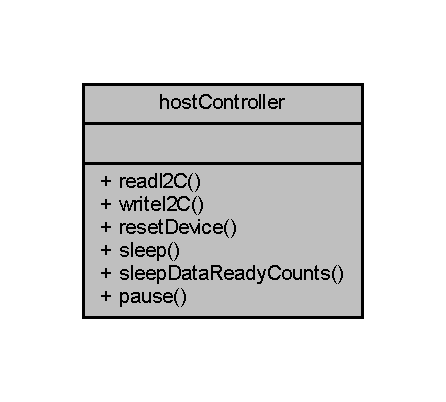
\includegraphics[width=214pt]{classhost_controller__coll__graph}
\end{center}
\end{figure}
\subsection*{Public Member Functions}
\begin{DoxyCompactItemize}
\item 
uint32\+\_\+t \mbox{\hyperlink{classhost_controller_a2bee6b3ec45fac241484f7dad943d8ed}{read\+I2C}} (uint8\+\_\+t address)
\begin{DoxyCompactList}\small\item\em method to read data from I2C port \end{DoxyCompactList}\item 
void \mbox{\hyperlink{classhost_controller_a7c4126810a72333e3ebe749159a0a516}{write\+I2C}} (uint8\+\_\+t address, uint32\+\_\+t data)
\begin{DoxyCompactList}\small\item\em method to write data from I2C port \end{DoxyCompactList}\item 
void \mbox{\hyperlink{classhost_controller_aa9f25eaf4a9bda5213c70ff91c261649}{reset\+Device}} ()
\begin{DoxyCompactList}\small\item\em send reset pulse to \mbox{\hyperlink{namespace_o_p_t3101}{O\+P\+T3101}} device Method used to send reset pulse to \mbox{\hyperlink{namespace_o_p_t3101}{O\+P\+T3101}} device \end{DoxyCompactList}\item 
void \mbox{\hyperlink{classhost_controller_a024c031559fade5da0ff7de491212dfe}{sleep}} (uint32\+\_\+t time\+In\+Milli\+Seconds)
\begin{DoxyCompactList}\small\item\em sleep host Method used to sleep or make host wait for a particular amount of time specified in milli\+Seconds \end{DoxyCompactList}\item 
void \mbox{\hyperlink{classhost_controller_aa678c25de9014a442ed33a4db695aeb3}{sleep\+Data\+Ready\+Counts}} (uint16\+\_\+t data\+Ready\+Counts)
\begin{DoxyCompactList}\small\item\em sleep host Method used to sleep or make host wait for a particular amount of time specified in number of data ready pulses from \mbox{\hyperlink{namespace_o_p_t3101}{O\+P\+T3101}} \end{DoxyCompactList}\item 
void \mbox{\hyperlink{classhost_controller_aead6dcbe7d02d5b2ae92b5cde1d99f05}{pause}} ()
\begin{DoxyCompactList}\small\item\em pause host Method used to make host wait for user input or interrupt. Useful for debug \end{DoxyCompactList}\end{DoxyCompactItemize}


\subsection{Detailed Description}
Generic implementation for host. 

As part of O\+P\+T3101\+S\+DK there are several host specific functions that need to be performed. Examples of such functions are writing or reading from I2C ports, sending reset pulse to \mbox{\hyperlink{namespace_o_p_t3101}{O\+P\+T3101}} device~\newline
 These implementations are very specific to the host on which the S\+DK is ported and run. ~\newline
 This abstract class provides a template with self explanatory method names which the users can override and implement their own functions. ~\newline
 Example code is provided for O\+P\+T3101\+E\+VM with implementations for a windows 10 PC. 

\subsection{Member Function Documentation}
\mbox{\Hypertarget{classhost_controller_aead6dcbe7d02d5b2ae92b5cde1d99f05}\label{classhost_controller_aead6dcbe7d02d5b2ae92b5cde1d99f05}} 
\index{host\+Controller@{host\+Controller}!pause@{pause}}
\index{pause@{pause}!host\+Controller@{host\+Controller}}
\subsubsection{\texorpdfstring{pause()}{pause()}}
{\footnotesize\ttfamily void host\+Controller\+::pause (\begin{DoxyParamCaption}{ }\end{DoxyParamCaption})}



pause host Method used to make host wait for user input or interrupt. Useful for debug 

\begin{DoxyReturn}{Returns}
Nothing 
\end{DoxyReturn}
{\bfseries Algorithm of the method is as follows} \mbox{\Hypertarget{classhost_controller_a2bee6b3ec45fac241484f7dad943d8ed}\label{classhost_controller_a2bee6b3ec45fac241484f7dad943d8ed}} 
\index{host\+Controller@{host\+Controller}!read\+I2C@{read\+I2C}}
\index{read\+I2C@{read\+I2C}!host\+Controller@{host\+Controller}}
\subsubsection{\texorpdfstring{read\+I2\+C()}{readI2C()}}
{\footnotesize\ttfamily uint32\+\_\+t host\+Controller\+::read\+I2C (\begin{DoxyParamCaption}\item[{uint8\+\_\+t}]{address }\end{DoxyParamCaption})}



method to read data from I2C port 


\begin{DoxyParams}[1]{Parameters}
\mbox{\tt in}  & {\em address;} & address is the I2C register address \\
\hline
\end{DoxyParams}
\begin{DoxyReturn}{Returns}
value; value read from I2C port for the address 
\end{DoxyReturn}
{\bfseries Algorithm of the method is as follows}


\begin{DoxyItemize}
\item Creates R\+E\+AD I2C command to send to h/w with address and data specified in arguments
\item Writes the R\+E\+AD I2C command to h/w
\item Waits and receives response from h/w
\item Converters the received string output from h/w to uint32\+\_\+t value
\item Returns the data in uint32\+\_\+t format 
\end{DoxyItemize}\mbox{\Hypertarget{classhost_controller_aa9f25eaf4a9bda5213c70ff91c261649}\label{classhost_controller_aa9f25eaf4a9bda5213c70ff91c261649}} 
\index{host\+Controller@{host\+Controller}!reset\+Device@{reset\+Device}}
\index{reset\+Device@{reset\+Device}!host\+Controller@{host\+Controller}}
\subsubsection{\texorpdfstring{reset\+Device()}{resetDevice()}}
{\footnotesize\ttfamily void host\+Controller\+::reset\+Device (\begin{DoxyParamCaption}{ }\end{DoxyParamCaption})}



send reset pulse to \mbox{\hyperlink{namespace_o_p_t3101}{O\+P\+T3101}} device Method used to send reset pulse to \mbox{\hyperlink{namespace_o_p_t3101}{O\+P\+T3101}} device 

\begin{DoxyReturn}{Returns}
Nothing 
\end{DoxyReturn}
{\bfseries Algorithm of the method is as follows}


\begin{DoxyItemize}
\item Creates a command which specifies host to send R\+E\+S\+ET Pulse to \mbox{\hyperlink{namespace_o_p_t3101}{O\+P\+T3101}} h/w ~\newline

\item Send the R\+E\+S\+ET command to the h/w 
\end{DoxyItemize}\mbox{\Hypertarget{classhost_controller_a024c031559fade5da0ff7de491212dfe}\label{classhost_controller_a024c031559fade5da0ff7de491212dfe}} 
\index{host\+Controller@{host\+Controller}!sleep@{sleep}}
\index{sleep@{sleep}!host\+Controller@{host\+Controller}}
\subsubsection{\texorpdfstring{sleep()}{sleep()}}
{\footnotesize\ttfamily void host\+Controller\+::sleep (\begin{DoxyParamCaption}\item[{uint32\+\_\+t}]{time\+In\+Milli\+Seconds }\end{DoxyParamCaption})}



sleep host Method used to sleep or make host wait for a particular amount of time specified in milli\+Seconds 


\begin{DoxyParams}[1]{Parameters}
\mbox{\tt in}  & {\em time\+In\+Milli\+Seconds;} & Time for which the host needs to sleep specified in milli\+Seconds \\
\hline
\end{DoxyParams}
\begin{DoxyReturn}{Returns}
Nothing 
\end{DoxyReturn}
{\bfseries Algorithm of the method is as follows}


\begin{DoxyItemize}
\item Sleeps for the time specified in the argument time\+In\+Milli\+Seconds 
\end{DoxyItemize}\mbox{\Hypertarget{classhost_controller_aa678c25de9014a442ed33a4db695aeb3}\label{classhost_controller_aa678c25de9014a442ed33a4db695aeb3}} 
\index{host\+Controller@{host\+Controller}!sleep\+Data\+Ready\+Counts@{sleep\+Data\+Ready\+Counts}}
\index{sleep\+Data\+Ready\+Counts@{sleep\+Data\+Ready\+Counts}!host\+Controller@{host\+Controller}}
\subsubsection{\texorpdfstring{sleep\+Data\+Ready\+Counts()}{sleepDataReadyCounts()}}
{\footnotesize\ttfamily void host\+Controller\+::sleep\+Data\+Ready\+Counts (\begin{DoxyParamCaption}\item[{uint16\+\_\+t}]{data\+Ready\+Counts }\end{DoxyParamCaption})}



sleep host Method used to sleep or make host wait for a particular amount of time specified in number of data ready pulses from \mbox{\hyperlink{namespace_o_p_t3101}{O\+P\+T3101}} 


\begin{DoxyParams}[1]{Parameters}
\mbox{\tt in}  & {\em data\+Ready\+Counts;} & Time for which the host needs to sleep specified data ready pulses from \mbox{\hyperlink{namespace_o_p_t3101}{O\+P\+T3101}} \\
\hline
\end{DoxyParams}
\begin{DoxyReturn}{Returns}
Nothing 
\end{DoxyReturn}
{\bfseries Algorithm of the method is as follows}
\begin{DoxyItemize}
\item Currently empty function needs to be implemented by user. Based on interrupts from data ready signal from \mbox{\hyperlink{namespace_o_p_t3101}{O\+P\+T3101}}, the host needs to count those pulses and wait until data\+Ready\+Counts have reached. 
\end{DoxyItemize}\mbox{\Hypertarget{classhost_controller_a7c4126810a72333e3ebe749159a0a516}\label{classhost_controller_a7c4126810a72333e3ebe749159a0a516}} 
\index{host\+Controller@{host\+Controller}!write\+I2C@{write\+I2C}}
\index{write\+I2C@{write\+I2C}!host\+Controller@{host\+Controller}}
\subsubsection{\texorpdfstring{write\+I2\+C()}{writeI2C()}}
{\footnotesize\ttfamily void host\+Controller\+::write\+I2C (\begin{DoxyParamCaption}\item[{uint8\+\_\+t}]{address,  }\item[{uint32\+\_\+t}]{data }\end{DoxyParamCaption})}



method to write data from I2C port 


\begin{DoxyParams}[1]{Parameters}
\mbox{\tt in}  & {\em address;} & address is the I2C register address \\
\hline
\mbox{\tt in}  & {\em data;} & data to write to I2C register \\
\hline
\end{DoxyParams}
\begin{DoxyReturn}{Returns}
Nothing 
\end{DoxyReturn}
{\bfseries Algorithm of the method is as follows}


\begin{DoxyItemize}
\item Creates W\+R\+I\+TE I2C command to send to h/w with address and data specified in arguments
\item Writes the W\+R\+I\+TE I2C command to h/w 
\end{DoxyItemize}

The documentation for this class was generated from the following files\+:\begin{DoxyCompactItemize}
\item 
C\+:/folders/d/scripts/cpp/\+O\+P\+T3101\+S\+D\+K/\+O\+P\+T3101\+S\+D\+K/\+O\+P\+T3101\+S\+D\+K/\mbox{\hyperlink{host_controller_8h}{host\+Controller.\+h}}\item 
C\+:/folders/d/scripts/cpp/\+O\+P\+T3101\+S\+D\+K/\+O\+P\+T3101\+S\+D\+K/\+O\+P\+T3101\+S\+D\+K/\mbox{\hyperlink{host_controller_8cpp}{host\+Controller.\+cpp}}\end{DoxyCompactItemize}

\hypertarget{classserial_1_1_i_o_exception}{}\section{serial\+:\+:I\+O\+Exception Class Reference}
\label{classserial_1_1_i_o_exception}\index{serial\+::\+I\+O\+Exception@{serial\+::\+I\+O\+Exception}}


{\ttfamily \#include $<$serial.\+h$>$}



Inheritance diagram for serial\+:\+:I\+O\+Exception\+:\nopagebreak
\begin{figure}[H]
\begin{center}
\leavevmode
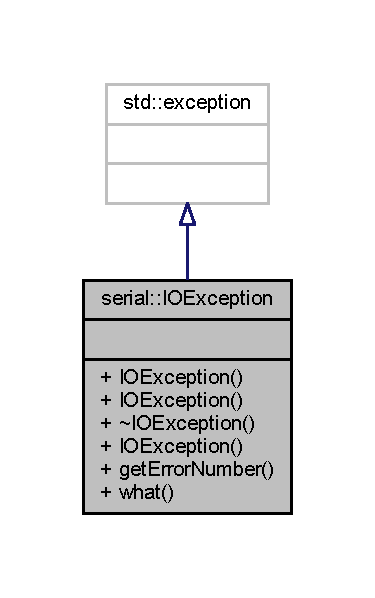
\includegraphics[width=180pt]{classserial_1_1_i_o_exception__inherit__graph}
\end{center}
\end{figure}


Collaboration diagram for serial\+:\+:I\+O\+Exception\+:\nopagebreak
\begin{figure}[H]
\begin{center}
\leavevmode
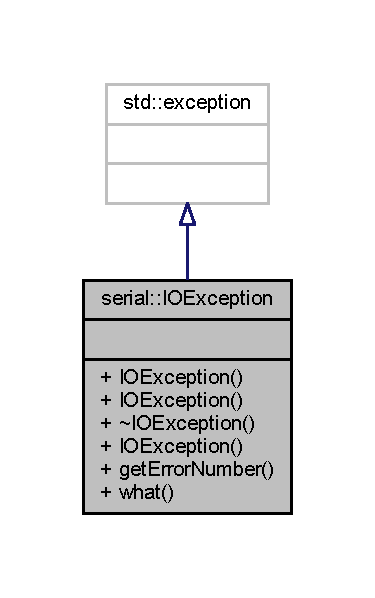
\includegraphics[width=180pt]{classserial_1_1_i_o_exception__coll__graph}
\end{center}
\end{figure}
\subsection*{Public Member Functions}
\begin{DoxyCompactItemize}
\item 
\mbox{\hyperlink{classserial_1_1_i_o_exception_acb2f2cf7a5cc8090945f6cbfcef3ef1e}{I\+O\+Exception}} (std\+::string file, int line, int errnum)
\item 
\mbox{\hyperlink{classserial_1_1_i_o_exception_acc1d2c650832cc8127f2cd777072b2cd}{I\+O\+Exception}} (std\+::string file, int line, const char $\ast$description)
\item 
virtual \mbox{\hyperlink{classserial_1_1_i_o_exception_a026ae2e6abc57c6069915f0f8c701390}{$\sim$\+I\+O\+Exception}} ()  throw ()
\item 
\mbox{\hyperlink{classserial_1_1_i_o_exception_af65196a71b800d11b5e5c367caf5b354}{I\+O\+Exception}} (const \mbox{\hyperlink{classserial_1_1_i_o_exception}{I\+O\+Exception}} \&other)
\item 
int \mbox{\hyperlink{classserial_1_1_i_o_exception_af6b35e13d3d212ab2f7ecbb28a231de4}{get\+Error\+Number}} () const
\item 
virtual const char $\ast$ \mbox{\hyperlink{classserial_1_1_i_o_exception_abd1b0ecb2f1a867ed7ade7c3f3b9dada}{what}} () const  throw ()
\end{DoxyCompactItemize}


\subsection{Constructor \& Destructor Documentation}
\mbox{\Hypertarget{classserial_1_1_i_o_exception_acb2f2cf7a5cc8090945f6cbfcef3ef1e}\label{classserial_1_1_i_o_exception_acb2f2cf7a5cc8090945f6cbfcef3ef1e}} 
\index{serial\+::\+I\+O\+Exception@{serial\+::\+I\+O\+Exception}!I\+O\+Exception@{I\+O\+Exception}}
\index{I\+O\+Exception@{I\+O\+Exception}!serial\+::\+I\+O\+Exception@{serial\+::\+I\+O\+Exception}}
\subsubsection{\texorpdfstring{I\+O\+Exception()}{IOException()}\hspace{0.1cm}{\footnotesize\ttfamily [1/3]}}
{\footnotesize\ttfamily serial\+::\+I\+O\+Exception\+::\+I\+O\+Exception (\begin{DoxyParamCaption}\item[{std\+::string}]{file,  }\item[{int}]{line,  }\item[{int}]{errnum }\end{DoxyParamCaption})\hspace{0.3cm}{\ttfamily [inline]}, {\ttfamily [explicit]}}

\mbox{\Hypertarget{classserial_1_1_i_o_exception_acc1d2c650832cc8127f2cd777072b2cd}\label{classserial_1_1_i_o_exception_acc1d2c650832cc8127f2cd777072b2cd}} 
\index{serial\+::\+I\+O\+Exception@{serial\+::\+I\+O\+Exception}!I\+O\+Exception@{I\+O\+Exception}}
\index{I\+O\+Exception@{I\+O\+Exception}!serial\+::\+I\+O\+Exception@{serial\+::\+I\+O\+Exception}}
\subsubsection{\texorpdfstring{I\+O\+Exception()}{IOException()}\hspace{0.1cm}{\footnotesize\ttfamily [2/3]}}
{\footnotesize\ttfamily serial\+::\+I\+O\+Exception\+::\+I\+O\+Exception (\begin{DoxyParamCaption}\item[{std\+::string}]{file,  }\item[{int}]{line,  }\item[{const char $\ast$}]{description }\end{DoxyParamCaption})\hspace{0.3cm}{\ttfamily [inline]}, {\ttfamily [explicit]}}

\mbox{\Hypertarget{classserial_1_1_i_o_exception_a026ae2e6abc57c6069915f0f8c701390}\label{classserial_1_1_i_o_exception_a026ae2e6abc57c6069915f0f8c701390}} 
\index{serial\+::\+I\+O\+Exception@{serial\+::\+I\+O\+Exception}!````~I\+O\+Exception@{$\sim$\+I\+O\+Exception}}
\index{````~I\+O\+Exception@{$\sim$\+I\+O\+Exception}!serial\+::\+I\+O\+Exception@{serial\+::\+I\+O\+Exception}}
\subsubsection{\texorpdfstring{$\sim$\+I\+O\+Exception()}{~IOException()}}
{\footnotesize\ttfamily virtual serial\+::\+I\+O\+Exception\+::$\sim$\+I\+O\+Exception (\begin{DoxyParamCaption}{ }\end{DoxyParamCaption}) throw  ) \hspace{0.3cm}{\ttfamily [inline]}, {\ttfamily [virtual]}}

\mbox{\Hypertarget{classserial_1_1_i_o_exception_af65196a71b800d11b5e5c367caf5b354}\label{classserial_1_1_i_o_exception_af65196a71b800d11b5e5c367caf5b354}} 
\index{serial\+::\+I\+O\+Exception@{serial\+::\+I\+O\+Exception}!I\+O\+Exception@{I\+O\+Exception}}
\index{I\+O\+Exception@{I\+O\+Exception}!serial\+::\+I\+O\+Exception@{serial\+::\+I\+O\+Exception}}
\subsubsection{\texorpdfstring{I\+O\+Exception()}{IOException()}\hspace{0.1cm}{\footnotesize\ttfamily [3/3]}}
{\footnotesize\ttfamily serial\+::\+I\+O\+Exception\+::\+I\+O\+Exception (\begin{DoxyParamCaption}\item[{const \mbox{\hyperlink{classserial_1_1_i_o_exception}{I\+O\+Exception}} \&}]{other }\end{DoxyParamCaption})\hspace{0.3cm}{\ttfamily [inline]}}



\subsection{Member Function Documentation}
\mbox{\Hypertarget{classserial_1_1_i_o_exception_af6b35e13d3d212ab2f7ecbb28a231de4}\label{classserial_1_1_i_o_exception_af6b35e13d3d212ab2f7ecbb28a231de4}} 
\index{serial\+::\+I\+O\+Exception@{serial\+::\+I\+O\+Exception}!get\+Error\+Number@{get\+Error\+Number}}
\index{get\+Error\+Number@{get\+Error\+Number}!serial\+::\+I\+O\+Exception@{serial\+::\+I\+O\+Exception}}
\subsubsection{\texorpdfstring{get\+Error\+Number()}{getErrorNumber()}}
{\footnotesize\ttfamily int serial\+::\+I\+O\+Exception\+::get\+Error\+Number (\begin{DoxyParamCaption}{ }\end{DoxyParamCaption}) const\hspace{0.3cm}{\ttfamily [inline]}}

\mbox{\Hypertarget{classserial_1_1_i_o_exception_abd1b0ecb2f1a867ed7ade7c3f3b9dada}\label{classserial_1_1_i_o_exception_abd1b0ecb2f1a867ed7ade7c3f3b9dada}} 
\index{serial\+::\+I\+O\+Exception@{serial\+::\+I\+O\+Exception}!what@{what}}
\index{what@{what}!serial\+::\+I\+O\+Exception@{serial\+::\+I\+O\+Exception}}
\subsubsection{\texorpdfstring{what()}{what()}}
{\footnotesize\ttfamily virtual const char$\ast$ serial\+::\+I\+O\+Exception\+::what (\begin{DoxyParamCaption}{ }\end{DoxyParamCaption}) const throw  ) \hspace{0.3cm}{\ttfamily [inline]}, {\ttfamily [virtual]}}



The documentation for this class was generated from the following file\+:\begin{DoxyCompactItemize}
\item 
C\+:/folders/d/scripts/cpp/\+O\+P\+T3101\+S\+D\+K/\+O\+P\+T3101\+S\+D\+K/\+O\+P\+T3101\+S\+D\+K/serial\+Lib/\mbox{\hyperlink{serial_8h}{serial.\+h}}\end{DoxyCompactItemize}

\hypertarget{classserial_1_1_millisecond_timer}{}\section{serial\+:\+:Millisecond\+Timer Class Reference}
\label{classserial_1_1_millisecond_timer}\index{serial\+::\+Millisecond\+Timer@{serial\+::\+Millisecond\+Timer}}


{\ttfamily \#include $<$unix.\+h$>$}



Collaboration diagram for serial\+:\+:Millisecond\+Timer\+:\nopagebreak
\begin{figure}[H]
\begin{center}
\leavevmode
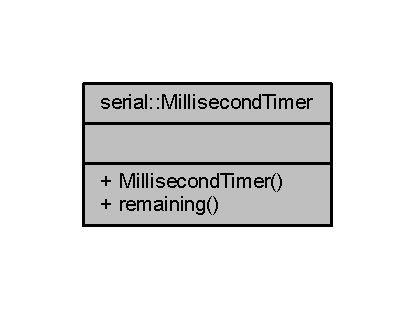
\includegraphics[width=199pt]{classserial_1_1_millisecond_timer__coll__graph}
\end{center}
\end{figure}
\subsection*{Public Member Functions}
\begin{DoxyCompactItemize}
\item 
\mbox{\hyperlink{classserial_1_1_millisecond_timer_aac5a60ab2fd6cbba430ba89eceffab86}{Millisecond\+Timer}} (const uint32\+\_\+t millis)
\item 
int64\+\_\+t \mbox{\hyperlink{classserial_1_1_millisecond_timer_a3786e2c6d8614adff0da39e1d1a2b0e3}{remaining}} ()
\end{DoxyCompactItemize}


\subsection{Constructor \& Destructor Documentation}
\mbox{\Hypertarget{classserial_1_1_millisecond_timer_aac5a60ab2fd6cbba430ba89eceffab86}\label{classserial_1_1_millisecond_timer_aac5a60ab2fd6cbba430ba89eceffab86}} 
\index{serial\+::\+Millisecond\+Timer@{serial\+::\+Millisecond\+Timer}!Millisecond\+Timer@{Millisecond\+Timer}}
\index{Millisecond\+Timer@{Millisecond\+Timer}!serial\+::\+Millisecond\+Timer@{serial\+::\+Millisecond\+Timer}}
\subsubsection{\texorpdfstring{Millisecond\+Timer()}{MillisecondTimer()}}
{\footnotesize\ttfamily Millisecond\+Timer\+::\+Millisecond\+Timer (\begin{DoxyParamCaption}\item[{const uint32\+\_\+t}]{millis }\end{DoxyParamCaption})}



\subsection{Member Function Documentation}
\mbox{\Hypertarget{classserial_1_1_millisecond_timer_a3786e2c6d8614adff0da39e1d1a2b0e3}\label{classserial_1_1_millisecond_timer_a3786e2c6d8614adff0da39e1d1a2b0e3}} 
\index{serial\+::\+Millisecond\+Timer@{serial\+::\+Millisecond\+Timer}!remaining@{remaining}}
\index{remaining@{remaining}!serial\+::\+Millisecond\+Timer@{serial\+::\+Millisecond\+Timer}}
\subsubsection{\texorpdfstring{remaining()}{remaining()}}
{\footnotesize\ttfamily int64\+\_\+t Millisecond\+Timer\+::remaining (\begin{DoxyParamCaption}{ }\end{DoxyParamCaption})}



The documentation for this class was generated from the following files\+:\begin{DoxyCompactItemize}
\item 
C\+:/folders/d/scripts/cpp/\+O\+P\+T3101\+S\+D\+K/\+O\+P\+T3101\+S\+D\+K/\+O\+P\+T3101\+S\+D\+K/serial\+Lib/\mbox{\hyperlink{unix_8h}{unix.\+h}}\item 
C\+:/folders/d/scripts/cpp/\+O\+P\+T3101\+S\+D\+K/\+O\+P\+T3101\+S\+D\+K/\+O\+P\+T3101\+S\+D\+K/serial\+Lib/\mbox{\hyperlink{unix_8cc}{unix.\+cc}}\end{DoxyCompactItemize}

\hypertarget{class_o_p_t3101_1_1phase_ambient_coff_c}{}\section{O\+P\+T3101\+:\+:phase\+Ambient\+CoffC Class Reference}
\label{class_o_p_t3101_1_1phase_ambient_coff_c}\index{O\+P\+T3101\+::phase\+Ambient\+CoffC@{O\+P\+T3101\+::phase\+Ambient\+CoffC}}


Class that holds ambient phase coefficient related registers and values.  




{\ttfamily \#include $<$O\+P\+T3101\+Design\+Coefficients.\+h$>$}



Collaboration diagram for O\+P\+T3101\+:\+:phase\+Ambient\+CoffC\+:\nopagebreak
\begin{figure}[H]
\begin{center}
\leavevmode
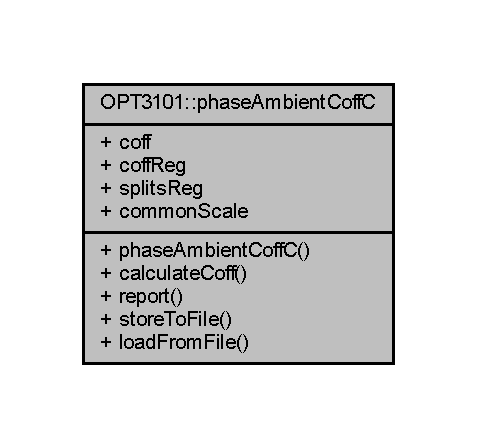
\includegraphics[width=229pt]{class_o_p_t3101_1_1phase_ambient_coff_c__coll__graph}
\end{center}
\end{figure}
\subsection*{Public Member Functions}
\begin{DoxyCompactItemize}
\item 
\mbox{\hyperlink{class_o_p_t3101_1_1phase_ambient_coff_c_aa32106a402df3ed93a73203634017953}{phase\+Ambient\+CoffC}} ()
\begin{DoxyCompactList}\small\item\em initializes the members to 0 \end{DoxyCompactList}\item 
void \mbox{\hyperlink{class_o_p_t3101_1_1phase_ambient_coff_c_ac8f4dfff191b0adc7be044f39500e242}{calculate\+Coff}} (uint16\+\_\+t freq\+Counter)
\begin{DoxyCompactList}\small\item\em Calculates the register settings for the phase ambient coefficient Calculates \mbox{\hyperlink{class_o_p_t3101_1_1phase_ambient_coff_c_a267c8f925dedeb8af97aba7ffae95da4}{O\+P\+T3101\+::phase\+Ambient\+Coff\+C\+::coff\+Reg}} and \mbox{\hyperlink{class_o_p_t3101_1_1phase_ambient_coff_c_abed8ff9971976201638badbda9fd4543}{O\+P\+T3101\+::phase\+Ambient\+Coff\+C\+::common\+Scale}} based on \mbox{\hyperlink{class_o_p_t3101_1_1phase_ambient_coff_c_af655f6704c4b3901b82a913f8a047258}{O\+P\+T3101\+::phase\+Ambient\+Coff\+C\+::coff}}. \end{DoxyCompactList}\item 
void \mbox{\hyperlink{class_o_p_t3101_1_1phase_ambient_coff_c_afba22e085a341c2d9b1add1532ea06a1}{report}} ()
\begin{DoxyCompactList}\small\item\em reports members of the instance Print the members of the class instance on screen \end{DoxyCompactList}\item 
void \mbox{\hyperlink{class_o_p_t3101_1_1phase_ambient_coff_c_ad5b439c7ab384c03fa540d2bc06c3352}{store\+To\+File}} (char $\ast$file\+Name)
\begin{DoxyCompactList}\small\item\em saves phase ambient coff values to file This methods saves the phase ambient coff values to a non-\/volatile memory. Storage/\+Restoration to/from non-\/volatile memory is important for factory calibration \end{DoxyCompactList}\item 
void \mbox{\hyperlink{class_o_p_t3101_1_1phase_ambient_coff_c_a41db9882facdbf3b437dcb54958b5763}{load\+From\+File}} (char $\ast$file\+Name)
\begin{DoxyCompactList}\small\item\em load phase ambient coff values from file This methods loads the phase ambient coff values to a non-\/volatile memory. Storage/\+Restoration to/from non-\/volatile memory is important for factory calibration \end{DoxyCompactList}\end{DoxyCompactItemize}
\subsection*{Public Attributes}
\begin{DoxyCompactItemize}
\item 
double \mbox{\hyperlink{class_o_p_t3101_1_1phase_ambient_coff_c_af655f6704c4b3901b82a913f8a047258}{coff}} \mbox{[}4\mbox{]}
\begin{DoxyCompactList}\small\item\em Coefficients stored in floating point precision. Since there are 4 sections the \mbox{\hyperlink{class_o_p_t3101_1_1phase_ambient_coff_c_af655f6704c4b3901b82a913f8a047258}{O\+P\+T3101\+::phase\+Ambient\+Coff\+C\+::coff}} is array of 4 elements. Units for this is \mbox{\hyperlink{class_o_p_t3101_1_1frame_data_af8661d11405953dc378ad4d7cb0f2db6}{O\+P\+T3101\+::frame\+Data\+::phase}} codes per unit \mbox{\hyperlink{class_o_p_t3101_1_1frame_data_a39ebf8bd06141bef6986e49013d03c35}{O\+P\+T3101\+::frame\+Data\+::ambient}} codes. \end{DoxyCompactList}\item 
uint8\+\_\+t \mbox{\hyperlink{class_o_p_t3101_1_1phase_ambient_coff_c_a267c8f925dedeb8af97aba7ffae95da4}{coff\+Reg}} \mbox{[}4\mbox{]}
\begin{DoxyCompactList}\small\item\em Coefficients value of \mbox{\hyperlink{class_o_p_t3101_1_1phase_ambient_coff_c_af655f6704c4b3901b82a913f8a047258}{O\+P\+T3101\+::phase\+Ambient\+Coff\+C\+::coff}} represented as 8 bit register values calculated by \mbox{\hyperlink{class_o_p_t3101_1_1phase_ambient_coff_c_ac8f4dfff191b0adc7be044f39500e242}{O\+P\+T3101\+::phase\+Ambient\+Coff\+C\+::calculate\+Coff}}. \end{DoxyCompactList}\item 
uint16\+\_\+t \mbox{\hyperlink{class_o_p_t3101_1_1phase_ambient_coff_c_a5a2e9d6a0622f02024eaa8a1d2ec0011}{splits\+Reg}} \mbox{[}3\mbox{]}
\begin{DoxyCompactList}\small\item\em Register entries for the split point for the P\+WL. Since there are 4 sections where are 3 split points to be set. Units for this is \mbox{\hyperlink{class_o_p_t3101_1_1frame_data_a39ebf8bd06141bef6986e49013d03c35}{O\+P\+T3101\+::frame\+Data\+::ambient}} codes. \end{DoxyCompactList}\item 
uint8\+\_\+t \mbox{\hyperlink{class_o_p_t3101_1_1phase_ambient_coff_c_abed8ff9971976201638badbda9fd4543}{common\+Scale}}
\begin{DoxyCompactList}\small\item\em Since there are 4 \mbox{\hyperlink{class_o_p_t3101_1_1phase_ambient_coff_c_af655f6704c4b3901b82a913f8a047258}{O\+P\+T3101\+::phase\+Ambient\+Coff\+C\+::coff}} to represent them as 8 bit register values a common scaling factor is required. This is calculated by method \mbox{\hyperlink{class_o_p_t3101_1_1phase_ambient_coff_c_ac8f4dfff191b0adc7be044f39500e242}{O\+P\+T3101\+::phase\+Ambient\+Coff\+C\+::calculate\+Coff}}. \end{DoxyCompactList}\end{DoxyCompactItemize}
\subsection*{Friends}
\begin{DoxyCompactItemize}
\item 
std\+::ostream \& \mbox{\hyperlink{class_o_p_t3101_1_1phase_ambient_coff_c_a3febbb121799f99cb3f3f6578b43fae9}{operator$<$$<$}} (std\+::ostream \&os, const \mbox{\hyperlink{class_o_p_t3101_1_1phase_ambient_coff_c}{phase\+Ambient\+CoffC}} $\ast$data)
\begin{DoxyCompactList}\small\item\em Operator overload to store class contents to a file Casts all the class members for file storage. \end{DoxyCompactList}\item 
std\+::istream \& \mbox{\hyperlink{class_o_p_t3101_1_1phase_ambient_coff_c_a1aec354cf48fdc653937a8168af6c78c}{operator$>$$>$}} (std\+::istream \&is, \mbox{\hyperlink{class_o_p_t3101_1_1phase_ambient_coff_c}{phase\+Ambient\+CoffC}} $\ast$data)
\begin{DoxyCompactList}\small\item\em Operator overload to load class contents to from a file Retrieves all the class members from a stored file. \end{DoxyCompactList}\end{DoxyCompactItemize}


\subsection{Detailed Description}
Class that holds ambient phase coefficient related registers and values. 

This is a class container that can hold phase offset ambient coefficients and related registers. Photo diodes has a phenomenon where the phase delay of modulated current generated by photo diode is dependent on the amount of ambient light falling on the photo diode. The effect observed on the system is that the phase reported by the system will be dependent on the amount of ambient light of the environment. ~\newline
 \mbox{\hyperlink{namespace_o_p_t3101}{O\+P\+T3101}} has compensation block for the same, which needs coefficients to be programmed. \mbox{\hyperlink{namespace_o_p_t3101}{O\+P\+T3101}} has a look up table based correction since the phenomenon in non-\/linear. The look-\/up table is a 4 way split P\+WL correction with 4 independent coefficients. The P\+WL correlation is between ambient A\+DC output and phase measured~\newline
 This class has members to contain the coefficients and the split points. 

\subsection{Constructor \& Destructor Documentation}
\mbox{\Hypertarget{class_o_p_t3101_1_1phase_ambient_coff_c_aa32106a402df3ed93a73203634017953}\label{class_o_p_t3101_1_1phase_ambient_coff_c_aa32106a402df3ed93a73203634017953}} 
\index{O\+P\+T3101\+::phase\+Ambient\+CoffC@{O\+P\+T3101\+::phase\+Ambient\+CoffC}!phase\+Ambient\+CoffC@{phase\+Ambient\+CoffC}}
\index{phase\+Ambient\+CoffC@{phase\+Ambient\+CoffC}!O\+P\+T3101\+::phase\+Ambient\+CoffC@{O\+P\+T3101\+::phase\+Ambient\+CoffC}}
\subsubsection{\texorpdfstring{phase\+Ambient\+Coff\+C()}{phaseAmbientCoffC()}}
{\footnotesize\ttfamily O\+P\+T3101\+::phase\+Ambient\+Coff\+C\+::phase\+Ambient\+CoffC (\begin{DoxyParamCaption}{ }\end{DoxyParamCaption})}



initializes the members to 0 

\begin{DoxyReturn}{Returns}
Nothing; 
\end{DoxyReturn}
{\bfseries Algorithm of the method is as follows}


\begin{DoxyItemize}
\item Serializes all the members and returns to the stream 
\end{DoxyItemize}

\subsection{Member Function Documentation}
\mbox{\Hypertarget{class_o_p_t3101_1_1phase_ambient_coff_c_ac8f4dfff191b0adc7be044f39500e242}\label{class_o_p_t3101_1_1phase_ambient_coff_c_ac8f4dfff191b0adc7be044f39500e242}} 
\index{O\+P\+T3101\+::phase\+Ambient\+CoffC@{O\+P\+T3101\+::phase\+Ambient\+CoffC}!calculate\+Coff@{calculate\+Coff}}
\index{calculate\+Coff@{calculate\+Coff}!O\+P\+T3101\+::phase\+Ambient\+CoffC@{O\+P\+T3101\+::phase\+Ambient\+CoffC}}
\subsubsection{\texorpdfstring{calculate\+Coff()}{calculateCoff()}}
{\footnotesize\ttfamily void O\+P\+T3101\+::phase\+Ambient\+Coff\+C\+::calculate\+Coff (\begin{DoxyParamCaption}\item[{uint16\+\_\+t}]{freq\+Counter }\end{DoxyParamCaption})}



Calculates the register settings for the phase ambient coefficient Calculates \mbox{\hyperlink{class_o_p_t3101_1_1phase_ambient_coff_c_a267c8f925dedeb8af97aba7ffae95da4}{O\+P\+T3101\+::phase\+Ambient\+Coff\+C\+::coff\+Reg}} and \mbox{\hyperlink{class_o_p_t3101_1_1phase_ambient_coff_c_abed8ff9971976201638badbda9fd4543}{O\+P\+T3101\+::phase\+Ambient\+Coff\+C\+::common\+Scale}} based on \mbox{\hyperlink{class_o_p_t3101_1_1phase_ambient_coff_c_af655f6704c4b3901b82a913f8a047258}{O\+P\+T3101\+::phase\+Ambient\+Coff\+C\+::coff}}. 


\begin{DoxyParams}[1]{Parameters}
\mbox{\tt in}  & {\em freq\+Counter;} & freq\+Counter is the count which represents the frequency from the Frequency correction block. This is read from register \mbox{\hyperlink{class_o_p_t3101_1_1registers_a0d343738560c0bc418f34b458735a811}{O\+P\+T3101\+::registers\+::freq\+\_\+count\+\_\+read\+\_\+reg}} \\
\hline
\end{DoxyParams}
\begin{DoxyReturn}{Returns}
Nothing; 
\end{DoxyReturn}
{\bfseries Algorithm of the method is as follows}


\begin{DoxyItemize}
\item Identifies max of absolute of \mbox{\hyperlink{class_o_p_t3101_1_1phase_ambient_coff_c_af655f6704c4b3901b82a913f8a047258}{O\+P\+T3101\+::phase\+Ambient\+Coff\+C\+::coff}} values ~\newline
~\newline
~\newline

\item scales the max coefficient with input frequency\+Count ~\newline
~\newline

\item Finds a \mbox{\hyperlink{class_o_p_t3101_1_1phase_ambient_coff_c_abed8ff9971976201638badbda9fd4543}{O\+P\+T3101\+::phase\+Ambient\+Coff\+C\+::common\+Scale}} which can fit the \mbox{\hyperlink{class_o_p_t3101_1_1phase_ambient_coff_c_af655f6704c4b3901b82a913f8a047258}{O\+P\+T3101\+::phase\+Ambient\+Coff\+C\+::coff}} to 8 bit registers
\item Finds \mbox{\hyperlink{class_o_p_t3101_1_1phase_ambient_coff_c_a267c8f925dedeb8af97aba7ffae95da4}{O\+P\+T3101\+::phase\+Ambient\+Coff\+C\+::coff\+Reg}} values (8 bit register values) based on \mbox{\hyperlink{class_o_p_t3101_1_1phase_ambient_coff_c_af655f6704c4b3901b82a913f8a047258}{O\+P\+T3101\+::phase\+Ambient\+Coff\+C\+::coff}} and \mbox{\hyperlink{class_o_p_t3101_1_1phase_ambient_coff_c_abed8ff9971976201638badbda9fd4543}{O\+P\+T3101\+::phase\+Ambient\+Coff\+C\+::common\+Scale}} 
\end{DoxyItemize}\mbox{\Hypertarget{class_o_p_t3101_1_1phase_ambient_coff_c_a41db9882facdbf3b437dcb54958b5763}\label{class_o_p_t3101_1_1phase_ambient_coff_c_a41db9882facdbf3b437dcb54958b5763}} 
\index{O\+P\+T3101\+::phase\+Ambient\+CoffC@{O\+P\+T3101\+::phase\+Ambient\+CoffC}!load\+From\+File@{load\+From\+File}}
\index{load\+From\+File@{load\+From\+File}!O\+P\+T3101\+::phase\+Ambient\+CoffC@{O\+P\+T3101\+::phase\+Ambient\+CoffC}}
\subsubsection{\texorpdfstring{load\+From\+File()}{loadFromFile()}}
{\footnotesize\ttfamily void O\+P\+T3101\+::phase\+Ambient\+Coff\+C\+::load\+From\+File (\begin{DoxyParamCaption}\item[{char $\ast$}]{file\+Name }\end{DoxyParamCaption})}



load phase ambient coff values from file This methods loads the phase ambient coff values to a non-\/volatile memory. Storage/\+Restoration to/from non-\/volatile memory is important for factory calibration 


\begin{DoxyParams}[1]{Parameters}
\mbox{\tt in}  & {\em file\+Name;} & Path and name of the file from where to load \\
\hline
\end{DoxyParams}
\begin{DoxyReturn}{Returns}
Nothing; 
\end{DoxyReturn}
{\bfseries Algorithm of the method is as follows}


\begin{DoxyItemize}
\item User needs to implement file load/restore based on host. 
\end{DoxyItemize}\mbox{\Hypertarget{class_o_p_t3101_1_1phase_ambient_coff_c_afba22e085a341c2d9b1add1532ea06a1}\label{class_o_p_t3101_1_1phase_ambient_coff_c_afba22e085a341c2d9b1add1532ea06a1}} 
\index{O\+P\+T3101\+::phase\+Ambient\+CoffC@{O\+P\+T3101\+::phase\+Ambient\+CoffC}!report@{report}}
\index{report@{report}!O\+P\+T3101\+::phase\+Ambient\+CoffC@{O\+P\+T3101\+::phase\+Ambient\+CoffC}}
\subsubsection{\texorpdfstring{report()}{report()}}
{\footnotesize\ttfamily void O\+P\+T3101\+::phase\+Ambient\+Coff\+C\+::report (\begin{DoxyParamCaption}{ }\end{DoxyParamCaption})}



reports members of the instance Print the members of the class instance on screen 

\begin{DoxyReturn}{Returns}
Nothing; 
\end{DoxyReturn}
{\bfseries Algorithm of the method is as follows}


\begin{DoxyItemize}
\item Prints all the members and values of members on screen. ~\newline

\item Prints all the members and values of members on screen. 
\end{DoxyItemize}\mbox{\Hypertarget{class_o_p_t3101_1_1phase_ambient_coff_c_ad5b439c7ab384c03fa540d2bc06c3352}\label{class_o_p_t3101_1_1phase_ambient_coff_c_ad5b439c7ab384c03fa540d2bc06c3352}} 
\index{O\+P\+T3101\+::phase\+Ambient\+CoffC@{O\+P\+T3101\+::phase\+Ambient\+CoffC}!store\+To\+File@{store\+To\+File}}
\index{store\+To\+File@{store\+To\+File}!O\+P\+T3101\+::phase\+Ambient\+CoffC@{O\+P\+T3101\+::phase\+Ambient\+CoffC}}
\subsubsection{\texorpdfstring{store\+To\+File()}{storeToFile()}}
{\footnotesize\ttfamily void O\+P\+T3101\+::phase\+Ambient\+Coff\+C\+::store\+To\+File (\begin{DoxyParamCaption}\item[{char $\ast$}]{file\+Name }\end{DoxyParamCaption})}



saves phase ambient coff values to file This methods saves the phase ambient coff values to a non-\/volatile memory. Storage/\+Restoration to/from non-\/volatile memory is important for factory calibration 


\begin{DoxyParams}[1]{Parameters}
\mbox{\tt in}  & {\em file\+Name;} & Path and name of the file to store \\
\hline
\end{DoxyParams}
\begin{DoxyReturn}{Returns}
Nothing; 
\end{DoxyReturn}
{\bfseries Algorithm of the method is as follows}


\begin{DoxyItemize}
\item User needs to implement file storage based on host. 
\end{DoxyItemize}

\subsection{Friends And Related Function Documentation}
\mbox{\Hypertarget{class_o_p_t3101_1_1phase_ambient_coff_c_a3febbb121799f99cb3f3f6578b43fae9}\label{class_o_p_t3101_1_1phase_ambient_coff_c_a3febbb121799f99cb3f3f6578b43fae9}} 
\index{O\+P\+T3101\+::phase\+Ambient\+CoffC@{O\+P\+T3101\+::phase\+Ambient\+CoffC}!operator$<$$<$@{operator$<$$<$}}
\index{operator$<$$<$@{operator$<$$<$}!O\+P\+T3101\+::phase\+Ambient\+CoffC@{O\+P\+T3101\+::phase\+Ambient\+CoffC}}
\subsubsection{\texorpdfstring{operator$<$$<$}{operator<<}}
{\footnotesize\ttfamily std\+::ostream\& operator$<$$<$ (\begin{DoxyParamCaption}\item[{std\+::ostream \&}]{os,  }\item[{const \mbox{\hyperlink{class_o_p_t3101_1_1phase_ambient_coff_c}{phase\+Ambient\+CoffC}} $\ast$}]{data }\end{DoxyParamCaption})\hspace{0.3cm}{\ttfamily [friend]}}



Operator overload to store class contents to a file Casts all the class members for file storage. 


\begin{DoxyParams}[1]{Parameters}
\mbox{\tt out}  & {\em os;} & os is data stream to serialize data \\
\hline
\mbox{\tt in}  & {\em data;} & data is pointer to the class to be serialized and stored \\
\hline
\end{DoxyParams}
\begin{DoxyReturn}{Returns}
std\+::ostream; Serialized std\+::ostream to be written to a file 
\end{DoxyReturn}
\mbox{\Hypertarget{class_o_p_t3101_1_1phase_ambient_coff_c_a1aec354cf48fdc653937a8168af6c78c}\label{class_o_p_t3101_1_1phase_ambient_coff_c_a1aec354cf48fdc653937a8168af6c78c}} 
\index{O\+P\+T3101\+::phase\+Ambient\+CoffC@{O\+P\+T3101\+::phase\+Ambient\+CoffC}!operator$>$$>$@{operator$>$$>$}}
\index{operator$>$$>$@{operator$>$$>$}!O\+P\+T3101\+::phase\+Ambient\+CoffC@{O\+P\+T3101\+::phase\+Ambient\+CoffC}}
\subsubsection{\texorpdfstring{operator$>$$>$}{operator>>}}
{\footnotesize\ttfamily std\+::istream\& operator$>$$>$ (\begin{DoxyParamCaption}\item[{std\+::istream \&}]{is,  }\item[{\mbox{\hyperlink{class_o_p_t3101_1_1phase_ambient_coff_c}{phase\+Ambient\+CoffC}} $\ast$}]{data }\end{DoxyParamCaption})\hspace{0.3cm}{\ttfamily [friend]}}



Operator overload to load class contents to from a file Retrieves all the class members from a stored file. 


\begin{DoxyParams}[1]{Parameters}
\mbox{\tt in}  & {\em is;} & is input stream from where the data is loaded \\
\hline
\mbox{\tt out}  & {\em data;} & data is pointer to the class to be restored \\
\hline
\end{DoxyParams}
\begin{DoxyReturn}{Returns}
std\+::istream; Serialized Input stream loaded from file 
\end{DoxyReturn}


\subsection{Member Data Documentation}
\mbox{\Hypertarget{class_o_p_t3101_1_1phase_ambient_coff_c_af655f6704c4b3901b82a913f8a047258}\label{class_o_p_t3101_1_1phase_ambient_coff_c_af655f6704c4b3901b82a913f8a047258}} 
\index{O\+P\+T3101\+::phase\+Ambient\+CoffC@{O\+P\+T3101\+::phase\+Ambient\+CoffC}!coff@{coff}}
\index{coff@{coff}!O\+P\+T3101\+::phase\+Ambient\+CoffC@{O\+P\+T3101\+::phase\+Ambient\+CoffC}}
\subsubsection{\texorpdfstring{coff}{coff}}
{\footnotesize\ttfamily double O\+P\+T3101\+::phase\+Ambient\+Coff\+C\+::coff\mbox{[}4\mbox{]}}



Coefficients stored in floating point precision. Since there are 4 sections the \mbox{\hyperlink{class_o_p_t3101_1_1phase_ambient_coff_c_af655f6704c4b3901b82a913f8a047258}{O\+P\+T3101\+::phase\+Ambient\+Coff\+C\+::coff}} is array of 4 elements. Units for this is \mbox{\hyperlink{class_o_p_t3101_1_1frame_data_af8661d11405953dc378ad4d7cb0f2db6}{O\+P\+T3101\+::frame\+Data\+::phase}} codes per unit \mbox{\hyperlink{class_o_p_t3101_1_1frame_data_a39ebf8bd06141bef6986e49013d03c35}{O\+P\+T3101\+::frame\+Data\+::ambient}} codes. 

\mbox{\Hypertarget{class_o_p_t3101_1_1phase_ambient_coff_c_a267c8f925dedeb8af97aba7ffae95da4}\label{class_o_p_t3101_1_1phase_ambient_coff_c_a267c8f925dedeb8af97aba7ffae95da4}} 
\index{O\+P\+T3101\+::phase\+Ambient\+CoffC@{O\+P\+T3101\+::phase\+Ambient\+CoffC}!coff\+Reg@{coff\+Reg}}
\index{coff\+Reg@{coff\+Reg}!O\+P\+T3101\+::phase\+Ambient\+CoffC@{O\+P\+T3101\+::phase\+Ambient\+CoffC}}
\subsubsection{\texorpdfstring{coff\+Reg}{coffReg}}
{\footnotesize\ttfamily uint8\+\_\+t O\+P\+T3101\+::phase\+Ambient\+Coff\+C\+::coff\+Reg\mbox{[}4\mbox{]}}



Coefficients value of \mbox{\hyperlink{class_o_p_t3101_1_1phase_ambient_coff_c_af655f6704c4b3901b82a913f8a047258}{O\+P\+T3101\+::phase\+Ambient\+Coff\+C\+::coff}} represented as 8 bit register values calculated by \mbox{\hyperlink{class_o_p_t3101_1_1phase_ambient_coff_c_ac8f4dfff191b0adc7be044f39500e242}{O\+P\+T3101\+::phase\+Ambient\+Coff\+C\+::calculate\+Coff}}. 

\mbox{\Hypertarget{class_o_p_t3101_1_1phase_ambient_coff_c_abed8ff9971976201638badbda9fd4543}\label{class_o_p_t3101_1_1phase_ambient_coff_c_abed8ff9971976201638badbda9fd4543}} 
\index{O\+P\+T3101\+::phase\+Ambient\+CoffC@{O\+P\+T3101\+::phase\+Ambient\+CoffC}!common\+Scale@{common\+Scale}}
\index{common\+Scale@{common\+Scale}!O\+P\+T3101\+::phase\+Ambient\+CoffC@{O\+P\+T3101\+::phase\+Ambient\+CoffC}}
\subsubsection{\texorpdfstring{common\+Scale}{commonScale}}
{\footnotesize\ttfamily uint8\+\_\+t O\+P\+T3101\+::phase\+Ambient\+Coff\+C\+::common\+Scale}



Since there are 4 \mbox{\hyperlink{class_o_p_t3101_1_1phase_ambient_coff_c_af655f6704c4b3901b82a913f8a047258}{O\+P\+T3101\+::phase\+Ambient\+Coff\+C\+::coff}} to represent them as 8 bit register values a common scaling factor is required. This is calculated by method \mbox{\hyperlink{class_o_p_t3101_1_1phase_ambient_coff_c_ac8f4dfff191b0adc7be044f39500e242}{O\+P\+T3101\+::phase\+Ambient\+Coff\+C\+::calculate\+Coff}}. 

\mbox{\Hypertarget{class_o_p_t3101_1_1phase_ambient_coff_c_a5a2e9d6a0622f02024eaa8a1d2ec0011}\label{class_o_p_t3101_1_1phase_ambient_coff_c_a5a2e9d6a0622f02024eaa8a1d2ec0011}} 
\index{O\+P\+T3101\+::phase\+Ambient\+CoffC@{O\+P\+T3101\+::phase\+Ambient\+CoffC}!splits\+Reg@{splits\+Reg}}
\index{splits\+Reg@{splits\+Reg}!O\+P\+T3101\+::phase\+Ambient\+CoffC@{O\+P\+T3101\+::phase\+Ambient\+CoffC}}
\subsubsection{\texorpdfstring{splits\+Reg}{splitsReg}}
{\footnotesize\ttfamily uint16\+\_\+t O\+P\+T3101\+::phase\+Ambient\+Coff\+C\+::splits\+Reg\mbox{[}3\mbox{]}}



Register entries for the split point for the P\+WL. Since there are 4 sections where are 3 split points to be set. Units for this is \mbox{\hyperlink{class_o_p_t3101_1_1frame_data_a39ebf8bd06141bef6986e49013d03c35}{O\+P\+T3101\+::frame\+Data\+::ambient}} codes. 



The documentation for this class was generated from the following files\+:\begin{DoxyCompactItemize}
\item 
C\+:/folders/d/scripts/cpp/\+O\+P\+T3101\+S\+D\+K/\+O\+P\+T3101\+S\+D\+K/\+O\+P\+T3101\+S\+D\+K/\mbox{\hyperlink{_o_p_t3101_design_coefficients_8h}{O\+P\+T3101\+Design\+Coefficients.\+h}}\item 
C\+:/folders/d/scripts/cpp/\+O\+P\+T3101\+S\+D\+K/\+O\+P\+T3101\+S\+D\+K/\+O\+P\+T3101\+S\+D\+K/\mbox{\hyperlink{_o_p_t3101_design_coefficients_8cpp}{O\+P\+T3101\+Design\+Coefficients.\+cpp}}\end{DoxyCompactItemize}

\hypertarget{class_o_p_t3101_1_1phase_offset_c}{}\section{O\+P\+T3101\+:\+:phase\+OffsetC Class Reference}
\label{class_o_p_t3101_1_1phase_offset_c}\index{O\+P\+T3101\+::phase\+OffsetC@{O\+P\+T3101\+::phase\+OffsetC}}


Class that holds phase offset register data.  




{\ttfamily \#include $<$O\+P\+T3101\+Phase\+Offset.\+h$>$}



Collaboration diagram for O\+P\+T3101\+:\+:phase\+OffsetC\+:\nopagebreak
\begin{figure}[H]
\begin{center}
\leavevmode
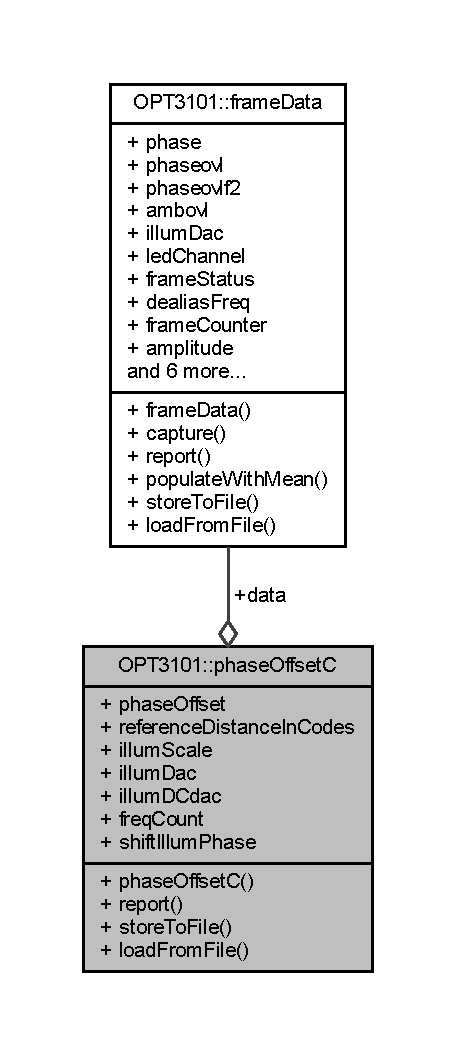
\includegraphics[width=219pt]{class_o_p_t3101_1_1phase_offset_c__coll__graph}
\end{center}
\end{figure}
\subsection*{Public Member Functions}
\begin{DoxyCompactItemize}
\item 
\mbox{\hyperlink{class_o_p_t3101_1_1phase_offset_c_af565b7d9f3261f8e9fc51c08a2f7339a}{phase\+OffsetC}} ()
\begin{DoxyCompactList}\small\item\em initializes the members to 0 \end{DoxyCompactList}\item 
void \mbox{\hyperlink{class_o_p_t3101_1_1phase_offset_c_a6baba22699fdb39d45adfd104a44534c}{report}} ()
\begin{DoxyCompactList}\small\item\em reports members of the instance Print the members of the class instance on screen \end{DoxyCompactList}\item 
void \mbox{\hyperlink{class_o_p_t3101_1_1phase_offset_c_ae542e328ed54d6e791c1350d878d1dd0}{store\+To\+File}} (char $\ast$file\+Name)
\begin{DoxyCompactList}\small\item\em store phase offset values to file This methods stores the phase offset values to a non-\/volatile memory. Storage to non-\/volatile memory is important to be able to calculate temperature coefficient \mbox{\hyperlink{class_o_p_t3101_1_1crosstalk_temp_coff_c}{O\+P\+T3101\+::crosstalk\+Temp\+CoffC}} \end{DoxyCompactList}\item 
void \mbox{\hyperlink{class_o_p_t3101_1_1phase_offset_c_ad6eeb78005b21ce0bd248829ae510045}{load\+From\+File}} (char $\ast$file\+Name)
\begin{DoxyCompactList}\small\item\em load phase offset values from file This methods loads the phase offset values to a non-\/volatile memory. Storage/\+Restoration to/from non-\/volatile memory is important to be able to calculate temperature coefficient \mbox{\hyperlink{class_o_p_t3101_1_1crosstalk_temp_coff_c}{O\+P\+T3101\+::crosstalk\+Temp\+CoffC}} \end{DoxyCompactList}\end{DoxyCompactItemize}
\subsection*{Public Attributes}
\begin{DoxyCompactItemize}
\item 
uint16\+\_\+t \mbox{\hyperlink{class_o_p_t3101_1_1phase_offset_c_addeef913546f1c431b4fd189478884f9}{phase\+Offset}}
\begin{DoxyCompactList}\small\item\em This it the 16 bit phase offset register value to be written to the device registers for correcting the delays and offsets. \end{DoxyCompactList}\item 
uint16\+\_\+t \mbox{\hyperlink{class_o_p_t3101_1_1phase_offset_c_ac77c406f9d3672254fa2b91e97a22d0c}{reference\+Distance\+In\+Codes}}
\begin{DoxyCompactList}\small\item\em Captures a snapshot of the distances measured in \mbox{\hyperlink{class_o_p_t3101_1_1frame_data_af8661d11405953dc378ad4d7cb0f2db6}{O\+P\+T3101\+::frame\+Data\+::phase}} codes used during calibration. \end{DoxyCompactList}\item 
uint8\+\_\+t \mbox{\hyperlink{class_o_p_t3101_1_1phase_offset_c_a687116f5b495ca2314afd1b4cbc9bf34}{illum\+Scale}}
\begin{DoxyCompactList}\small\item\em Captures the illumination scale used during phase offset measurement. \end{DoxyCompactList}\item 
uint8\+\_\+t \mbox{\hyperlink{class_o_p_t3101_1_1phase_offset_c_a606c3c6697150e9f2672c7f7ad3d08ea}{illum\+Dac}}
\begin{DoxyCompactList}\small\item\em Captures the illumination current setting used during phase offset measurement. \end{DoxyCompactList}\item 
uint8\+\_\+t \mbox{\hyperlink{class_o_p_t3101_1_1phase_offset_c_a99bd3c6d218a562c98d2a842db48aaab}{illum\+D\+Cdac}}
\begin{DoxyCompactList}\small\item\em Captures the illumination DC current setting used during phase offset measurement. \end{DoxyCompactList}\item 
uint16\+\_\+t \mbox{\hyperlink{class_o_p_t3101_1_1phase_offset_c_ab95e4dde3ea8b0ad825d315160fe33ca}{freq\+Count}}
\begin{DoxyCompactList}\small\item\em Captures the frequency Count register \mbox{\hyperlink{class_o_p_t3101_1_1registers_a0d343738560c0bc418f34b458735a811}{O\+P\+T3101\+::registers\+::freq\+\_\+count\+\_\+read\+\_\+reg}} during phase offset measurement. \end{DoxyCompactList}\item 
uint8\+\_\+t \mbox{\hyperlink{class_o_p_t3101_1_1phase_offset_c_a1977598d500c18fdd2ba58cbfd8789b9}{shift\+Illum\+Phase}}
\begin{DoxyCompactList}\small\item\em Captures the register \mbox{\hyperlink{class_o_p_t3101_1_1registers_a18539cc6fd63ce4f504fcf16b1e48f31}{O\+P\+T3101\+::registers\+::shift\+\_\+illum\+\_\+phase}} during phase offset measurement. \end{DoxyCompactList}\item 
\mbox{\hyperlink{class_o_p_t3101_1_1frame_data}{frame\+Data}} \mbox{\hyperlink{class_o_p_t3101_1_1phase_offset_c_a2db3531b8b3c643bae7af9db0e1fd040}{data}}
\begin{DoxyCompactList}\small\item\em Captures the \mbox{\hyperlink{class_o_p_t3101_1_1frame_data}{O\+P\+T3101\+::frame\+Data}} used to calculate the \mbox{\hyperlink{class_o_p_t3101_1_1phase_offset_c_addeef913546f1c431b4fd189478884f9}{O\+P\+T3101\+::phase\+Offset\+C\+::phase\+Offset}} register. \end{DoxyCompactList}\end{DoxyCompactItemize}
\subsection*{Friends}
\begin{DoxyCompactItemize}
\item 
std\+::ostream \& \mbox{\hyperlink{class_o_p_t3101_1_1phase_offset_c_a14c7935315901f4bd7c15982b88da40a}{operator$<$$<$}} (std\+::ostream \&os, const \mbox{\hyperlink{class_o_p_t3101_1_1phase_offset_c}{phase\+OffsetC}} $\ast$\mbox{\hyperlink{class_o_p_t3101_1_1phase_offset_c_a2db3531b8b3c643bae7af9db0e1fd040}{data}})
\begin{DoxyCompactList}\small\item\em Operator overload to store class contents to a file Casts all the class members for file storage. \end{DoxyCompactList}\item 
std\+::istream \& \mbox{\hyperlink{class_o_p_t3101_1_1phase_offset_c_afa58bc00875bb33c432f672980242427}{operator$>$$>$}} (std\+::istream \&is, \mbox{\hyperlink{class_o_p_t3101_1_1phase_offset_c}{phase\+OffsetC}} $\ast$\mbox{\hyperlink{class_o_p_t3101_1_1phase_offset_c_a2db3531b8b3c643bae7af9db0e1fd040}{data}})
\begin{DoxyCompactList}\small\item\em Operator overload to load class contents to from a file Retreives all the class members from a stored file. \end{DoxyCompactList}\end{DoxyCompactItemize}


\subsection{Detailed Description}
Class that holds phase offset register data. 

The class contains the phase offset calibration registers and related snapshot from the device settings. Phase offset calibration is an important factory calibration that needs to be performed on every unit. The calibration is important to remove all the offsets and delays and read accurate distance or phase. The calibration involves having a target at a known distance and setting up offset register so that the device reads distance as expected. This class besides capturing the register settings also holds critical snapshot from device for analysis and debug. 

\subsection{Constructor \& Destructor Documentation}
\mbox{\Hypertarget{class_o_p_t3101_1_1phase_offset_c_af565b7d9f3261f8e9fc51c08a2f7339a}\label{class_o_p_t3101_1_1phase_offset_c_af565b7d9f3261f8e9fc51c08a2f7339a}} 
\index{O\+P\+T3101\+::phase\+OffsetC@{O\+P\+T3101\+::phase\+OffsetC}!phase\+OffsetC@{phase\+OffsetC}}
\index{phase\+OffsetC@{phase\+OffsetC}!O\+P\+T3101\+::phase\+OffsetC@{O\+P\+T3101\+::phase\+OffsetC}}
\subsubsection{\texorpdfstring{phase\+Offset\+C()}{phaseOffsetC()}}
{\footnotesize\ttfamily O\+P\+T3101\+::phase\+Offset\+C\+::phase\+OffsetC (\begin{DoxyParamCaption}{ }\end{DoxyParamCaption})}



initializes the members to 0 

\begin{DoxyReturn}{Returns}
Nothing; 
\end{DoxyReturn}
{\bfseries Algorithm of the method is as follows}


\begin{DoxyItemize}
\item Initializes all members to 0 
\end{DoxyItemize}

\subsection{Member Function Documentation}
\mbox{\Hypertarget{class_o_p_t3101_1_1phase_offset_c_ad6eeb78005b21ce0bd248829ae510045}\label{class_o_p_t3101_1_1phase_offset_c_ad6eeb78005b21ce0bd248829ae510045}} 
\index{O\+P\+T3101\+::phase\+OffsetC@{O\+P\+T3101\+::phase\+OffsetC}!load\+From\+File@{load\+From\+File}}
\index{load\+From\+File@{load\+From\+File}!O\+P\+T3101\+::phase\+OffsetC@{O\+P\+T3101\+::phase\+OffsetC}}
\subsubsection{\texorpdfstring{load\+From\+File()}{loadFromFile()}}
{\footnotesize\ttfamily void O\+P\+T3101\+::phase\+Offset\+C\+::load\+From\+File (\begin{DoxyParamCaption}\item[{char $\ast$}]{file\+Name }\end{DoxyParamCaption})}



load phase offset values from file This methods loads the phase offset values to a non-\/volatile memory. Storage/\+Restoration to/from non-\/volatile memory is important to be able to calculate temperature coefficient \mbox{\hyperlink{class_o_p_t3101_1_1crosstalk_temp_coff_c}{O\+P\+T3101\+::crosstalk\+Temp\+CoffC}} 


\begin{DoxyParams}[1]{Parameters}
\mbox{\tt in}  & {\em file\+Name;} & Path and name of the file from where the crosstalk values are loaded \\
\hline
\end{DoxyParams}
\begin{DoxyReturn}{Returns}
Nothing; 
\end{DoxyReturn}
{\bfseries Algorithm of the method is as follows}


\begin{DoxyItemize}
\item User needs to implement file load/restore based on host. 
\end{DoxyItemize}\mbox{\Hypertarget{class_o_p_t3101_1_1phase_offset_c_a6baba22699fdb39d45adfd104a44534c}\label{class_o_p_t3101_1_1phase_offset_c_a6baba22699fdb39d45adfd104a44534c}} 
\index{O\+P\+T3101\+::phase\+OffsetC@{O\+P\+T3101\+::phase\+OffsetC}!report@{report}}
\index{report@{report}!O\+P\+T3101\+::phase\+OffsetC@{O\+P\+T3101\+::phase\+OffsetC}}
\subsubsection{\texorpdfstring{report()}{report()}}
{\footnotesize\ttfamily void O\+P\+T3101\+::phase\+Offset\+C\+::report (\begin{DoxyParamCaption}{ }\end{DoxyParamCaption})}



reports members of the instance Print the members of the class instance on screen 

\begin{DoxyReturn}{Returns}
Nothing; 
\end{DoxyReturn}

\begin{DoxyItemize}
\item Prints all the members and values of members on screen. ~\newline

\item Prints all the members and values of members on screen. 
\end{DoxyItemize}\mbox{\Hypertarget{class_o_p_t3101_1_1phase_offset_c_ae542e328ed54d6e791c1350d878d1dd0}\label{class_o_p_t3101_1_1phase_offset_c_ae542e328ed54d6e791c1350d878d1dd0}} 
\index{O\+P\+T3101\+::phase\+OffsetC@{O\+P\+T3101\+::phase\+OffsetC}!store\+To\+File@{store\+To\+File}}
\index{store\+To\+File@{store\+To\+File}!O\+P\+T3101\+::phase\+OffsetC@{O\+P\+T3101\+::phase\+OffsetC}}
\subsubsection{\texorpdfstring{store\+To\+File()}{storeToFile()}}
{\footnotesize\ttfamily void O\+P\+T3101\+::phase\+Offset\+C\+::store\+To\+File (\begin{DoxyParamCaption}\item[{char $\ast$}]{file\+Name }\end{DoxyParamCaption})}



store phase offset values to file This methods stores the phase offset values to a non-\/volatile memory. Storage to non-\/volatile memory is important to be able to calculate temperature coefficient \mbox{\hyperlink{class_o_p_t3101_1_1crosstalk_temp_coff_c}{O\+P\+T3101\+::crosstalk\+Temp\+CoffC}} 


\begin{DoxyParams}[1]{Parameters}
\mbox{\tt in}  & {\em file\+Name;} & Path and name of the file to capture the crosstalk values to \\
\hline
\end{DoxyParams}
\begin{DoxyReturn}{Returns}
Nothing; 
\end{DoxyReturn}
{\bfseries Algorithm of the method is as follows}


\begin{DoxyItemize}
\item User needs to implement file storage based on host. 
\end{DoxyItemize}

\subsection{Friends And Related Function Documentation}
\mbox{\Hypertarget{class_o_p_t3101_1_1phase_offset_c_a14c7935315901f4bd7c15982b88da40a}\label{class_o_p_t3101_1_1phase_offset_c_a14c7935315901f4bd7c15982b88da40a}} 
\index{O\+P\+T3101\+::phase\+OffsetC@{O\+P\+T3101\+::phase\+OffsetC}!operator$<$$<$@{operator$<$$<$}}
\index{operator$<$$<$@{operator$<$$<$}!O\+P\+T3101\+::phase\+OffsetC@{O\+P\+T3101\+::phase\+OffsetC}}
\subsubsection{\texorpdfstring{operator$<$$<$}{operator<<}}
{\footnotesize\ttfamily std\+::ostream\& operator$<$$<$ (\begin{DoxyParamCaption}\item[{std\+::ostream \&}]{os,  }\item[{const \mbox{\hyperlink{class_o_p_t3101_1_1phase_offset_c}{phase\+OffsetC}} $\ast$}]{data }\end{DoxyParamCaption})\hspace{0.3cm}{\ttfamily [friend]}}



Operator overload to store class contents to a file Casts all the class members for file storage. 


\begin{DoxyParams}[1]{Parameters}
\mbox{\tt out}  & {\em os;} & os is data stream to serialize data \\
\hline
\mbox{\tt in}  & {\em data;} & data is pointer to the class to be serialized and stored \\
\hline
\end{DoxyParams}
\begin{DoxyReturn}{Returns}
std\+::ostream; Serialized std\+::ostream to be written to a file 
\end{DoxyReturn}
\mbox{\Hypertarget{class_o_p_t3101_1_1phase_offset_c_afa58bc00875bb33c432f672980242427}\label{class_o_p_t3101_1_1phase_offset_c_afa58bc00875bb33c432f672980242427}} 
\index{O\+P\+T3101\+::phase\+OffsetC@{O\+P\+T3101\+::phase\+OffsetC}!operator$>$$>$@{operator$>$$>$}}
\index{operator$>$$>$@{operator$>$$>$}!O\+P\+T3101\+::phase\+OffsetC@{O\+P\+T3101\+::phase\+OffsetC}}
\subsubsection{\texorpdfstring{operator$>$$>$}{operator>>}}
{\footnotesize\ttfamily std\+::istream\& operator$>$$>$ (\begin{DoxyParamCaption}\item[{std\+::istream \&}]{is,  }\item[{\mbox{\hyperlink{class_o_p_t3101_1_1phase_offset_c}{phase\+OffsetC}} $\ast$}]{data }\end{DoxyParamCaption})\hspace{0.3cm}{\ttfamily [friend]}}



Operator overload to load class contents to from a file Retreives all the class members from a stored file. 


\begin{DoxyParams}[1]{Parameters}
\mbox{\tt in}  & {\em is;} & is input stream from where the data is loaded \\
\hline
\mbox{\tt out}  & {\em data;} & data is pointer to the class to be restored \\
\hline
\end{DoxyParams}
\begin{DoxyReturn}{Returns}
std\+::istream; Serialized Input stream loaded from file 
\end{DoxyReturn}


\subsection{Member Data Documentation}
\mbox{\Hypertarget{class_o_p_t3101_1_1phase_offset_c_a2db3531b8b3c643bae7af9db0e1fd040}\label{class_o_p_t3101_1_1phase_offset_c_a2db3531b8b3c643bae7af9db0e1fd040}} 
\index{O\+P\+T3101\+::phase\+OffsetC@{O\+P\+T3101\+::phase\+OffsetC}!data@{data}}
\index{data@{data}!O\+P\+T3101\+::phase\+OffsetC@{O\+P\+T3101\+::phase\+OffsetC}}
\subsubsection{\texorpdfstring{data}{data}}
{\footnotesize\ttfamily \mbox{\hyperlink{class_o_p_t3101_1_1frame_data}{frame\+Data}} O\+P\+T3101\+::phase\+Offset\+C\+::data}



Captures the \mbox{\hyperlink{class_o_p_t3101_1_1frame_data}{O\+P\+T3101\+::frame\+Data}} used to calculate the \mbox{\hyperlink{class_o_p_t3101_1_1phase_offset_c_addeef913546f1c431b4fd189478884f9}{O\+P\+T3101\+::phase\+Offset\+C\+::phase\+Offset}} register. 

\mbox{\Hypertarget{class_o_p_t3101_1_1phase_offset_c_ab95e4dde3ea8b0ad825d315160fe33ca}\label{class_o_p_t3101_1_1phase_offset_c_ab95e4dde3ea8b0ad825d315160fe33ca}} 
\index{O\+P\+T3101\+::phase\+OffsetC@{O\+P\+T3101\+::phase\+OffsetC}!freq\+Count@{freq\+Count}}
\index{freq\+Count@{freq\+Count}!O\+P\+T3101\+::phase\+OffsetC@{O\+P\+T3101\+::phase\+OffsetC}}
\subsubsection{\texorpdfstring{freq\+Count}{freqCount}}
{\footnotesize\ttfamily uint16\+\_\+t O\+P\+T3101\+::phase\+Offset\+C\+::freq\+Count}



Captures the frequency Count register \mbox{\hyperlink{class_o_p_t3101_1_1registers_a0d343738560c0bc418f34b458735a811}{O\+P\+T3101\+::registers\+::freq\+\_\+count\+\_\+read\+\_\+reg}} during phase offset measurement. 

\mbox{\Hypertarget{class_o_p_t3101_1_1phase_offset_c_a606c3c6697150e9f2672c7f7ad3d08ea}\label{class_o_p_t3101_1_1phase_offset_c_a606c3c6697150e9f2672c7f7ad3d08ea}} 
\index{O\+P\+T3101\+::phase\+OffsetC@{O\+P\+T3101\+::phase\+OffsetC}!illum\+Dac@{illum\+Dac}}
\index{illum\+Dac@{illum\+Dac}!O\+P\+T3101\+::phase\+OffsetC@{O\+P\+T3101\+::phase\+OffsetC}}
\subsubsection{\texorpdfstring{illum\+Dac}{illumDac}}
{\footnotesize\ttfamily uint8\+\_\+t O\+P\+T3101\+::phase\+Offset\+C\+::illum\+Dac}



Captures the illumination current setting used during phase offset measurement. 

\mbox{\Hypertarget{class_o_p_t3101_1_1phase_offset_c_a99bd3c6d218a562c98d2a842db48aaab}\label{class_o_p_t3101_1_1phase_offset_c_a99bd3c6d218a562c98d2a842db48aaab}} 
\index{O\+P\+T3101\+::phase\+OffsetC@{O\+P\+T3101\+::phase\+OffsetC}!illum\+D\+Cdac@{illum\+D\+Cdac}}
\index{illum\+D\+Cdac@{illum\+D\+Cdac}!O\+P\+T3101\+::phase\+OffsetC@{O\+P\+T3101\+::phase\+OffsetC}}
\subsubsection{\texorpdfstring{illum\+D\+Cdac}{illumDCdac}}
{\footnotesize\ttfamily uint8\+\_\+t O\+P\+T3101\+::phase\+Offset\+C\+::illum\+D\+Cdac}



Captures the illumination DC current setting used during phase offset measurement. 

\mbox{\Hypertarget{class_o_p_t3101_1_1phase_offset_c_a687116f5b495ca2314afd1b4cbc9bf34}\label{class_o_p_t3101_1_1phase_offset_c_a687116f5b495ca2314afd1b4cbc9bf34}} 
\index{O\+P\+T3101\+::phase\+OffsetC@{O\+P\+T3101\+::phase\+OffsetC}!illum\+Scale@{illum\+Scale}}
\index{illum\+Scale@{illum\+Scale}!O\+P\+T3101\+::phase\+OffsetC@{O\+P\+T3101\+::phase\+OffsetC}}
\subsubsection{\texorpdfstring{illum\+Scale}{illumScale}}
{\footnotesize\ttfamily uint8\+\_\+t O\+P\+T3101\+::phase\+Offset\+C\+::illum\+Scale}



Captures the illumination scale used during phase offset measurement. 

\mbox{\Hypertarget{class_o_p_t3101_1_1phase_offset_c_addeef913546f1c431b4fd189478884f9}\label{class_o_p_t3101_1_1phase_offset_c_addeef913546f1c431b4fd189478884f9}} 
\index{O\+P\+T3101\+::phase\+OffsetC@{O\+P\+T3101\+::phase\+OffsetC}!phase\+Offset@{phase\+Offset}}
\index{phase\+Offset@{phase\+Offset}!O\+P\+T3101\+::phase\+OffsetC@{O\+P\+T3101\+::phase\+OffsetC}}
\subsubsection{\texorpdfstring{phase\+Offset}{phaseOffset}}
{\footnotesize\ttfamily uint16\+\_\+t O\+P\+T3101\+::phase\+Offset\+C\+::phase\+Offset}



This it the 16 bit phase offset register value to be written to the device registers for correcting the delays and offsets. 

\mbox{\Hypertarget{class_o_p_t3101_1_1phase_offset_c_ac77c406f9d3672254fa2b91e97a22d0c}\label{class_o_p_t3101_1_1phase_offset_c_ac77c406f9d3672254fa2b91e97a22d0c}} 
\index{O\+P\+T3101\+::phase\+OffsetC@{O\+P\+T3101\+::phase\+OffsetC}!reference\+Distance\+In\+Codes@{reference\+Distance\+In\+Codes}}
\index{reference\+Distance\+In\+Codes@{reference\+Distance\+In\+Codes}!O\+P\+T3101\+::phase\+OffsetC@{O\+P\+T3101\+::phase\+OffsetC}}
\subsubsection{\texorpdfstring{reference\+Distance\+In\+Codes}{referenceDistanceInCodes}}
{\footnotesize\ttfamily uint16\+\_\+t O\+P\+T3101\+::phase\+Offset\+C\+::reference\+Distance\+In\+Codes}



Captures a snapshot of the distances measured in \mbox{\hyperlink{class_o_p_t3101_1_1frame_data_af8661d11405953dc378ad4d7cb0f2db6}{O\+P\+T3101\+::frame\+Data\+::phase}} codes used during calibration. 

\mbox{\Hypertarget{class_o_p_t3101_1_1phase_offset_c_a1977598d500c18fdd2ba58cbfd8789b9}\label{class_o_p_t3101_1_1phase_offset_c_a1977598d500c18fdd2ba58cbfd8789b9}} 
\index{O\+P\+T3101\+::phase\+OffsetC@{O\+P\+T3101\+::phase\+OffsetC}!shift\+Illum\+Phase@{shift\+Illum\+Phase}}
\index{shift\+Illum\+Phase@{shift\+Illum\+Phase}!O\+P\+T3101\+::phase\+OffsetC@{O\+P\+T3101\+::phase\+OffsetC}}
\subsubsection{\texorpdfstring{shift\+Illum\+Phase}{shiftIllumPhase}}
{\footnotesize\ttfamily uint8\+\_\+t O\+P\+T3101\+::phase\+Offset\+C\+::shift\+Illum\+Phase}



Captures the register \mbox{\hyperlink{class_o_p_t3101_1_1registers_a18539cc6fd63ce4f504fcf16b1e48f31}{O\+P\+T3101\+::registers\+::shift\+\_\+illum\+\_\+phase}} during phase offset measurement. 



The documentation for this class was generated from the following files\+:\begin{DoxyCompactItemize}
\item 
C\+:/folders/d/scripts/cpp/\+O\+P\+T3101\+S\+D\+K/\+O\+P\+T3101\+S\+D\+K/\+O\+P\+T3101\+S\+D\+K/\mbox{\hyperlink{_o_p_t3101_phase_offset_8h}{O\+P\+T3101\+Phase\+Offset.\+h}}\item 
C\+:/folders/d/scripts/cpp/\+O\+P\+T3101\+S\+D\+K/\+O\+P\+T3101\+S\+D\+K/\+O\+P\+T3101\+S\+D\+K/\mbox{\hyperlink{_o_p_t3101_phase_offset_8cpp}{O\+P\+T3101\+Phase\+Offset.\+cpp}}\end{DoxyCompactItemize}

\hypertarget{class_o_p_t3101_1_1phase_temp_coff_c}{}\section{O\+P\+T3101\+:\+:phase\+Temp\+CoffC Class Reference}
\label{class_o_p_t3101_1_1phase_temp_coff_c}\index{O\+P\+T3101\+::phase\+Temp\+CoffC@{O\+P\+T3101\+::phase\+Temp\+CoffC}}


Class that holds phase temperature coefficient related registers and values.  




{\ttfamily \#include $<$O\+P\+T3101\+Design\+Coefficients.\+h$>$}



Collaboration diagram for O\+P\+T3101\+:\+:phase\+Temp\+CoffC\+:\nopagebreak
\begin{figure}[H]
\begin{center}
\leavevmode
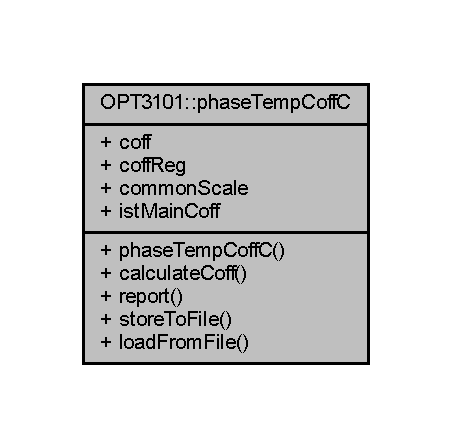
\includegraphics[width=217pt]{class_o_p_t3101_1_1phase_temp_coff_c__coll__graph}
\end{center}
\end{figure}
\subsection*{Public Member Functions}
\begin{DoxyCompactItemize}
\item 
\mbox{\hyperlink{class_o_p_t3101_1_1phase_temp_coff_c_a537d187395d87831e0004e333b1e0e94}{phase\+Temp\+CoffC}} ()
\begin{DoxyCompactList}\small\item\em initializes the members to 0 \end{DoxyCompactList}\item 
void \mbox{\hyperlink{class_o_p_t3101_1_1phase_temp_coff_c_a6a9ce25c87c81782b999e28c0a63a6af}{calculate\+Coff}} (\mbox{\hyperlink{class_o_p_t3101_1_1frame_data}{frame\+Data}} $\ast$frame\+Data0, \mbox{\hyperlink{class_o_p_t3101_1_1frame_data}{frame\+Data}} $\ast$frame\+Data1, bool \mbox{\hyperlink{class_o_p_t3101_1_1phase_temp_coff_c_abcd691cfc4678e3588bc1b38600632e7}{ist\+Main\+Coff}}=true)
\begin{DoxyCompactList}\small\item\em calculates the phase temp coff \end{DoxyCompactList}\item 
void \mbox{\hyperlink{class_o_p_t3101_1_1phase_temp_coff_c_af41bc218f81c9bfe8ae00e0bc6a64f4f}{report}} ()
\begin{DoxyCompactList}\small\item\em reports members of the instance Print the members of the class instance on screen \end{DoxyCompactList}\item 
void \mbox{\hyperlink{class_o_p_t3101_1_1phase_temp_coff_c_a05f0376e59830c4c81b37dc2042237e6}{store\+To\+File}} (char $\ast$file\+Name)
\begin{DoxyCompactList}\small\item\em saves phase temp coff values to file This methods saves the phase temp coff values to a non-\/volatile memory. Storage/\+Restoration to/from non-\/volatile memory is important for factory calibration \end{DoxyCompactList}\item 
void \mbox{\hyperlink{class_o_p_t3101_1_1phase_temp_coff_c_a26e1e98384b8d69f1f8bb8f3cd88071f}{load\+From\+File}} (char $\ast$file\+Name)
\begin{DoxyCompactList}\small\item\em load phase temp coff values from file This methods loads the phase temp coff values to a non-\/volatile memory. Storage/\+Restoration to/from non-\/volatile memory is important for factory calibration \end{DoxyCompactList}\end{DoxyCompactItemize}
\subsection*{Public Attributes}
\begin{DoxyCompactItemize}
\item 
double \mbox{\hyperlink{class_o_p_t3101_1_1phase_temp_coff_c_ade7d29c7cac1e63af7910eec0ec38043}{coff}}
\begin{DoxyCompactList}\small\item\em Coefficient stores in floating point precision.\+Units for this measurement is \mbox{\hyperlink{class_o_p_t3101_1_1frame_data_af8661d11405953dc378ad4d7cb0f2db6}{O\+P\+T3101\+::frame\+Data\+::phase}} codes (16 bit level) codes change per unit of temperature sensor codes (\mbox{\hyperlink{class_o_p_t3101_1_1registers_a3dfd8d81d4cb04d274007deb7c6122fc}{O\+P\+T3101\+::registers\+::tmain}} or \mbox{\hyperlink{class_o_p_t3101_1_1registers_a8a097a41ecdf2b98226c4a3a92121c12}{O\+P\+T3101\+::registers\+::tillum}} based on \mbox{\hyperlink{class_o_p_t3101_1_1phase_temp_coff_c_abcd691cfc4678e3588bc1b38600632e7}{O\+P\+T3101\+::phase\+Temp\+Coff\+C\+::ist\+Main\+Coff}}. \end{DoxyCompactList}\item 
uint16\+\_\+t \mbox{\hyperlink{class_o_p_t3101_1_1phase_temp_coff_c_a69e1782e097ce7ab761e4e55b5206f2e}{coff\+Reg}}
\begin{DoxyCompactList}\small\item\em Coefficient value of \mbox{\hyperlink{class_o_p_t3101_1_1phase_temp_coff_c_ade7d29c7cac1e63af7910eec0ec38043}{O\+P\+T3101\+::phase\+Temp\+Coff\+C\+::coff}} represented as 16bit register setting. \end{DoxyCompactList}\item 
uint8\+\_\+t \mbox{\hyperlink{class_o_p_t3101_1_1phase_temp_coff_c_a0f7646d71d058bc5354ac8f14270fcf3}{common\+Scale}}
\begin{DoxyCompactList}\small\item\em Common scale of \mbox{\hyperlink{class_o_p_t3101_1_1phase_temp_coff_c_a69e1782e097ce7ab761e4e55b5206f2e}{O\+P\+T3101\+::phase\+Temp\+Coff\+C\+::coff\+Reg}} calculated based on various \mbox{\hyperlink{class_o_p_t3101_1_1phase_temp_coff_c}{O\+P\+T3101\+::phase\+Temp\+CoffC}} class instances. This is calculated by \mbox{\hyperlink{class_o_p_t3101_1_1calibration_c_a5ca75c8e4d7818a90cacc0471522b365}{O\+P\+T3101\+::calibration\+C\+::find\+Phase\+Temp\+Register\+Values}} during production calibration. \end{DoxyCompactList}\item 
bool \mbox{\hyperlink{class_o_p_t3101_1_1phase_temp_coff_c_abcd691cfc4678e3588bc1b38600632e7}{ist\+Main\+Coff}}
\begin{DoxyCompactList}\small\item\em Flag which determines if the coefficient was obtained using \mbox{\hyperlink{class_o_p_t3101_1_1registers_a3dfd8d81d4cb04d274007deb7c6122fc}{O\+P\+T3101\+::registers\+::tmain}} difference or \mbox{\hyperlink{class_o_p_t3101_1_1registers_a8a097a41ecdf2b98226c4a3a92121c12}{O\+P\+T3101\+::registers\+::tillum}}. \end{DoxyCompactList}\end{DoxyCompactItemize}
\subsection*{Friends}
\begin{DoxyCompactItemize}
\item 
std\+::ostream \& \mbox{\hyperlink{class_o_p_t3101_1_1phase_temp_coff_c_a2d7a662f1af9735bc8cae566975afbec}{operator$<$$<$}} (std\+::ostream \&os, const \mbox{\hyperlink{class_o_p_t3101_1_1phase_temp_coff_c}{phase\+Temp\+CoffC}} $\ast$data)
\begin{DoxyCompactList}\small\item\em Operator overload to store class contents to a file Casts all the class members for file storage. \end{DoxyCompactList}\item 
std\+::istream \& \mbox{\hyperlink{class_o_p_t3101_1_1phase_temp_coff_c_aaf30671f3ce159d515fd178309007701}{operator$>$$>$}} (std\+::istream \&is, \mbox{\hyperlink{class_o_p_t3101_1_1phase_temp_coff_c}{phase\+Temp\+CoffC}} $\ast$data)
\begin{DoxyCompactList}\small\item\em Operator overload to load class contents to from a file Retrieves all the class members from a stored file. \end{DoxyCompactList}\end{DoxyCompactItemize}


\subsection{Detailed Description}
Class that holds phase temperature coefficient related registers and values. 

This is a class container that can hold phase/phase offset temperature coefficients and related register values. \mbox{\hyperlink{namespace_o_p_t3101}{O\+P\+T3101}} A\+FE phase measurement drifts over temperature. This drift is primarily due to change in delay in the path of the TX channels. The drift will show up in \mbox{\hyperlink{class_o_p_t3101_1_1frame_data_af8661d11405953dc378ad4d7cb0f2db6}{O\+P\+T3101\+::frame\+Data\+::phase}} measurement which will translate to error in measurement.~\newline
 \mbox{\hyperlink{namespace_o_p_t3101}{O\+P\+T3101}} has mechanism to compensate the output for this drift, for which phase temperature coefficient is required. Either internal temp sensor or external temperature sensor can be used to compensate for this. This class acts as a temporary storage of phase temp coefficients and related registers. Calculations have to be made on the phase offsets and frame data, coefficients to transform them to register settings. Instances of \mbox{\hyperlink{class_o_p_t3101_1_1frame_data}{O\+P\+T3101\+::frame\+Data}} taken at different temperature will be used to calculate these coefficients and registers. 

\subsection{Constructor \& Destructor Documentation}
\mbox{\Hypertarget{class_o_p_t3101_1_1phase_temp_coff_c_a537d187395d87831e0004e333b1e0e94}\label{class_o_p_t3101_1_1phase_temp_coff_c_a537d187395d87831e0004e333b1e0e94}} 
\index{O\+P\+T3101\+::phase\+Temp\+CoffC@{O\+P\+T3101\+::phase\+Temp\+CoffC}!phase\+Temp\+CoffC@{phase\+Temp\+CoffC}}
\index{phase\+Temp\+CoffC@{phase\+Temp\+CoffC}!O\+P\+T3101\+::phase\+Temp\+CoffC@{O\+P\+T3101\+::phase\+Temp\+CoffC}}
\subsubsection{\texorpdfstring{phase\+Temp\+Coff\+C()}{phaseTempCoffC()}}
{\footnotesize\ttfamily O\+P\+T3101\+::phase\+Temp\+Coff\+C\+::phase\+Temp\+CoffC (\begin{DoxyParamCaption}{ }\end{DoxyParamCaption})}



initializes the members to 0 

\begin{DoxyReturn}{Returns}
Nothing; 
\end{DoxyReturn}
{\bfseries Algorithm of the method is as follows}


\begin{DoxyItemize}
\item Initializes all members to 0. Sets \mbox{\hyperlink{class_o_p_t3101_1_1phase_temp_coff_c_abcd691cfc4678e3588bc1b38600632e7}{O\+P\+T3101\+::phase\+Temp\+Coff\+C\+::ist\+Main\+Coff}} to true 
\end{DoxyItemize}

\subsection{Member Function Documentation}
\mbox{\Hypertarget{class_o_p_t3101_1_1phase_temp_coff_c_a6a9ce25c87c81782b999e28c0a63a6af}\label{class_o_p_t3101_1_1phase_temp_coff_c_a6a9ce25c87c81782b999e28c0a63a6af}} 
\index{O\+P\+T3101\+::phase\+Temp\+CoffC@{O\+P\+T3101\+::phase\+Temp\+CoffC}!calculate\+Coff@{calculate\+Coff}}
\index{calculate\+Coff@{calculate\+Coff}!O\+P\+T3101\+::phase\+Temp\+CoffC@{O\+P\+T3101\+::phase\+Temp\+CoffC}}
\subsubsection{\texorpdfstring{calculate\+Coff()}{calculateCoff()}}
{\footnotesize\ttfamily void O\+P\+T3101\+::phase\+Temp\+Coff\+C\+::calculate\+Coff (\begin{DoxyParamCaption}\item[{\mbox{\hyperlink{class_o_p_t3101_1_1frame_data}{O\+P\+T3101\+::frame\+Data}} $\ast$}]{frame\+Data0,  }\item[{\mbox{\hyperlink{class_o_p_t3101_1_1frame_data}{O\+P\+T3101\+::frame\+Data}} $\ast$}]{frame\+Data1,  }\item[{bool}]{ist\+Main\+Coff = {\ttfamily true} }\end{DoxyParamCaption})}



calculates the phase temp coff 


\begin{DoxyParams}[1]{Parameters}
\mbox{\tt in}  & {\em frame\+Data0;} & Pointer to frame data \mbox{\hyperlink{class_o_p_t3101_1_1frame_data}{O\+P\+T3101\+::frame\+Data}} instance measured at a lower temperature \\
\hline
\mbox{\tt in}  & {\em frame\+Data1;} & Pointer to frame data \mbox{\hyperlink{class_o_p_t3101_1_1frame_data}{O\+P\+T3101\+::frame\+Data}} instance measured at a higher temperature \\
\hline
\mbox{\tt in}  & {\em ist\+Main\+Coff;} & ist\+Main\+Coff specifies if the calculation should be done with Tmain Coff \\
\hline
\end{DoxyParams}
\begin{DoxyReturn}{Returns}
Nothing; 
\end{DoxyReturn}
{\bfseries Algorithm of the method is as follows}


\begin{DoxyItemize}
\item Makes the data base circular to avoid errorneous high slope measurements
\item Assigns \mbox{\hyperlink{class_o_p_t3101_1_1phase_temp_coff_c_abcd691cfc4678e3588bc1b38600632e7}{O\+P\+T3101\+::phase\+Temp\+Coff\+C\+::ist\+Main\+Coff}} to the value assigned by argument
\item Calculates the double precision \mbox{\hyperlink{class_o_p_t3101_1_1phase_temp_coff_c_ade7d29c7cac1e63af7910eec0ec38043}{O\+P\+T3101\+::phase\+Temp\+Coff\+C\+::coff}} by finding difference between \mbox{\hyperlink{class_o_p_t3101_1_1frame_data_af8661d11405953dc378ad4d7cb0f2db6}{O\+P\+T3101\+::frame\+Data\+::phase}} divided by delta \mbox{\hyperlink{class_o_p_t3101_1_1frame_data_ae75ca7e9fa494b4d711eb070d5cab45b}{O\+P\+T3101\+::frame\+Data\+::tmain}} or \mbox{\hyperlink{class_o_p_t3101_1_1frame_data_aeb1934ab0ac8d1f846cf166ef26ceb75}{O\+P\+T3101\+::frame\+Data\+::tillum}} based on input flag
\item {\bfseries Warning\+:} Makes the \mbox{\hyperlink{class_o_p_t3101_1_1phase_temp_coff_c_ade7d29c7cac1e63af7910eec0ec38043}{O\+P\+T3101\+::phase\+Temp\+Coff\+C\+::coff}} 0 if the \mbox{\hyperlink{class_o_p_t3101_1_1frame_data_ae75ca7e9fa494b4d711eb070d5cab45b}{O\+P\+T3101\+::frame\+Data\+::tmain}} or \mbox{\hyperlink{class_o_p_t3101_1_1frame_data_aeb1934ab0ac8d1f846cf166ef26ceb75}{O\+P\+T3101\+::frame\+Data\+::tillum}} are same for both the input arguments 
\end{DoxyItemize}\mbox{\Hypertarget{class_o_p_t3101_1_1phase_temp_coff_c_a26e1e98384b8d69f1f8bb8f3cd88071f}\label{class_o_p_t3101_1_1phase_temp_coff_c_a26e1e98384b8d69f1f8bb8f3cd88071f}} 
\index{O\+P\+T3101\+::phase\+Temp\+CoffC@{O\+P\+T3101\+::phase\+Temp\+CoffC}!load\+From\+File@{load\+From\+File}}
\index{load\+From\+File@{load\+From\+File}!O\+P\+T3101\+::phase\+Temp\+CoffC@{O\+P\+T3101\+::phase\+Temp\+CoffC}}
\subsubsection{\texorpdfstring{load\+From\+File()}{loadFromFile()}}
{\footnotesize\ttfamily void O\+P\+T3101\+::phase\+Temp\+Coff\+C\+::load\+From\+File (\begin{DoxyParamCaption}\item[{char $\ast$}]{file\+Name }\end{DoxyParamCaption})}



load phase temp coff values from file This methods loads the phase temp coff values to a non-\/volatile memory. Storage/\+Restoration to/from non-\/volatile memory is important for factory calibration 


\begin{DoxyParams}[1]{Parameters}
\mbox{\tt in}  & {\em file\+Name;} & Path and name of the file from where to load \\
\hline
\end{DoxyParams}
\begin{DoxyReturn}{Returns}
Nothing; 
\end{DoxyReturn}
{\bfseries Algorithm of the method is as follows}


\begin{DoxyItemize}
\item User needs to implement file load/restore based on host. 
\end{DoxyItemize}\mbox{\Hypertarget{class_o_p_t3101_1_1phase_temp_coff_c_af41bc218f81c9bfe8ae00e0bc6a64f4f}\label{class_o_p_t3101_1_1phase_temp_coff_c_af41bc218f81c9bfe8ae00e0bc6a64f4f}} 
\index{O\+P\+T3101\+::phase\+Temp\+CoffC@{O\+P\+T3101\+::phase\+Temp\+CoffC}!report@{report}}
\index{report@{report}!O\+P\+T3101\+::phase\+Temp\+CoffC@{O\+P\+T3101\+::phase\+Temp\+CoffC}}
\subsubsection{\texorpdfstring{report()}{report()}}
{\footnotesize\ttfamily void O\+P\+T3101\+::phase\+Temp\+Coff\+C\+::report (\begin{DoxyParamCaption}{ }\end{DoxyParamCaption})}



reports members of the instance Print the members of the class instance on screen 

\begin{DoxyReturn}{Returns}
Nothing; 
\end{DoxyReturn}
{\bfseries Algorithm of the method is as follows}


\begin{DoxyItemize}
\item Prints all the members and values of members on screen. ~\newline

\item Prints all the members and values of members on screen. 
\end{DoxyItemize}\mbox{\Hypertarget{class_o_p_t3101_1_1phase_temp_coff_c_a05f0376e59830c4c81b37dc2042237e6}\label{class_o_p_t3101_1_1phase_temp_coff_c_a05f0376e59830c4c81b37dc2042237e6}} 
\index{O\+P\+T3101\+::phase\+Temp\+CoffC@{O\+P\+T3101\+::phase\+Temp\+CoffC}!store\+To\+File@{store\+To\+File}}
\index{store\+To\+File@{store\+To\+File}!O\+P\+T3101\+::phase\+Temp\+CoffC@{O\+P\+T3101\+::phase\+Temp\+CoffC}}
\subsubsection{\texorpdfstring{store\+To\+File()}{storeToFile()}}
{\footnotesize\ttfamily void O\+P\+T3101\+::phase\+Temp\+Coff\+C\+::store\+To\+File (\begin{DoxyParamCaption}\item[{char $\ast$}]{file\+Name }\end{DoxyParamCaption})}



saves phase temp coff values to file This methods saves the phase temp coff values to a non-\/volatile memory. Storage/\+Restoration to/from non-\/volatile memory is important for factory calibration 


\begin{DoxyParams}[1]{Parameters}
\mbox{\tt in}  & {\em file\+Name;} & Path and name of the file to store \\
\hline
\end{DoxyParams}
\begin{DoxyReturn}{Returns}
Nothing; 
\end{DoxyReturn}
{\bfseries Algorithm of the method is as follows}


\begin{DoxyItemize}
\item User needs to implement file storage based on host. 
\end{DoxyItemize}

\subsection{Friends And Related Function Documentation}
\mbox{\Hypertarget{class_o_p_t3101_1_1phase_temp_coff_c_a2d7a662f1af9735bc8cae566975afbec}\label{class_o_p_t3101_1_1phase_temp_coff_c_a2d7a662f1af9735bc8cae566975afbec}} 
\index{O\+P\+T3101\+::phase\+Temp\+CoffC@{O\+P\+T3101\+::phase\+Temp\+CoffC}!operator$<$$<$@{operator$<$$<$}}
\index{operator$<$$<$@{operator$<$$<$}!O\+P\+T3101\+::phase\+Temp\+CoffC@{O\+P\+T3101\+::phase\+Temp\+CoffC}}
\subsubsection{\texorpdfstring{operator$<$$<$}{operator<<}}
{\footnotesize\ttfamily std\+::ostream\& operator$<$$<$ (\begin{DoxyParamCaption}\item[{std\+::ostream \&}]{os,  }\item[{const \mbox{\hyperlink{class_o_p_t3101_1_1phase_temp_coff_c}{phase\+Temp\+CoffC}} $\ast$}]{data }\end{DoxyParamCaption})\hspace{0.3cm}{\ttfamily [friend]}}



Operator overload to store class contents to a file Casts all the class members for file storage. 


\begin{DoxyParams}[1]{Parameters}
\mbox{\tt out}  & {\em os;} & os is data stream to serialize data \\
\hline
\mbox{\tt in}  & {\em data;} & data is pointer to the class to be serialized and stored \\
\hline
\end{DoxyParams}
\begin{DoxyReturn}{Returns}
std\+::ostream; Serialized std\+::ostream to be written to a file 
\end{DoxyReturn}
\mbox{\Hypertarget{class_o_p_t3101_1_1phase_temp_coff_c_aaf30671f3ce159d515fd178309007701}\label{class_o_p_t3101_1_1phase_temp_coff_c_aaf30671f3ce159d515fd178309007701}} 
\index{O\+P\+T3101\+::phase\+Temp\+CoffC@{O\+P\+T3101\+::phase\+Temp\+CoffC}!operator$>$$>$@{operator$>$$>$}}
\index{operator$>$$>$@{operator$>$$>$}!O\+P\+T3101\+::phase\+Temp\+CoffC@{O\+P\+T3101\+::phase\+Temp\+CoffC}}
\subsubsection{\texorpdfstring{operator$>$$>$}{operator>>}}
{\footnotesize\ttfamily std\+::istream\& operator$>$$>$ (\begin{DoxyParamCaption}\item[{std\+::istream \&}]{is,  }\item[{\mbox{\hyperlink{class_o_p_t3101_1_1phase_temp_coff_c}{phase\+Temp\+CoffC}} $\ast$}]{data }\end{DoxyParamCaption})\hspace{0.3cm}{\ttfamily [friend]}}



Operator overload to load class contents to from a file Retrieves all the class members from a stored file. 


\begin{DoxyParams}[1]{Parameters}
\mbox{\tt in}  & {\em is;} & is input stream from where the data is loaded \\
\hline
\mbox{\tt out}  & {\em data;} & data is pointer to the class to be restored \\
\hline
\end{DoxyParams}
\begin{DoxyReturn}{Returns}
std\+::istream; Serialized Input stream loaded from file 
\end{DoxyReturn}


\subsection{Member Data Documentation}
\mbox{\Hypertarget{class_o_p_t3101_1_1phase_temp_coff_c_ade7d29c7cac1e63af7910eec0ec38043}\label{class_o_p_t3101_1_1phase_temp_coff_c_ade7d29c7cac1e63af7910eec0ec38043}} 
\index{O\+P\+T3101\+::phase\+Temp\+CoffC@{O\+P\+T3101\+::phase\+Temp\+CoffC}!coff@{coff}}
\index{coff@{coff}!O\+P\+T3101\+::phase\+Temp\+CoffC@{O\+P\+T3101\+::phase\+Temp\+CoffC}}
\subsubsection{\texorpdfstring{coff}{coff}}
{\footnotesize\ttfamily double O\+P\+T3101\+::phase\+Temp\+Coff\+C\+::coff}



Coefficient stores in floating point precision.\+Units for this measurement is \mbox{\hyperlink{class_o_p_t3101_1_1frame_data_af8661d11405953dc378ad4d7cb0f2db6}{O\+P\+T3101\+::frame\+Data\+::phase}} codes (16 bit level) codes change per unit of temperature sensor codes (\mbox{\hyperlink{class_o_p_t3101_1_1registers_a3dfd8d81d4cb04d274007deb7c6122fc}{O\+P\+T3101\+::registers\+::tmain}} or \mbox{\hyperlink{class_o_p_t3101_1_1registers_a8a097a41ecdf2b98226c4a3a92121c12}{O\+P\+T3101\+::registers\+::tillum}} based on \mbox{\hyperlink{class_o_p_t3101_1_1phase_temp_coff_c_abcd691cfc4678e3588bc1b38600632e7}{O\+P\+T3101\+::phase\+Temp\+Coff\+C\+::ist\+Main\+Coff}}. 

\mbox{\Hypertarget{class_o_p_t3101_1_1phase_temp_coff_c_a69e1782e097ce7ab761e4e55b5206f2e}\label{class_o_p_t3101_1_1phase_temp_coff_c_a69e1782e097ce7ab761e4e55b5206f2e}} 
\index{O\+P\+T3101\+::phase\+Temp\+CoffC@{O\+P\+T3101\+::phase\+Temp\+CoffC}!coff\+Reg@{coff\+Reg}}
\index{coff\+Reg@{coff\+Reg}!O\+P\+T3101\+::phase\+Temp\+CoffC@{O\+P\+T3101\+::phase\+Temp\+CoffC}}
\subsubsection{\texorpdfstring{coff\+Reg}{coffReg}}
{\footnotesize\ttfamily uint16\+\_\+t O\+P\+T3101\+::phase\+Temp\+Coff\+C\+::coff\+Reg}



Coefficient value of \mbox{\hyperlink{class_o_p_t3101_1_1phase_temp_coff_c_ade7d29c7cac1e63af7910eec0ec38043}{O\+P\+T3101\+::phase\+Temp\+Coff\+C\+::coff}} represented as 16bit register setting. 

\mbox{\Hypertarget{class_o_p_t3101_1_1phase_temp_coff_c_a0f7646d71d058bc5354ac8f14270fcf3}\label{class_o_p_t3101_1_1phase_temp_coff_c_a0f7646d71d058bc5354ac8f14270fcf3}} 
\index{O\+P\+T3101\+::phase\+Temp\+CoffC@{O\+P\+T3101\+::phase\+Temp\+CoffC}!common\+Scale@{common\+Scale}}
\index{common\+Scale@{common\+Scale}!O\+P\+T3101\+::phase\+Temp\+CoffC@{O\+P\+T3101\+::phase\+Temp\+CoffC}}
\subsubsection{\texorpdfstring{common\+Scale}{commonScale}}
{\footnotesize\ttfamily uint8\+\_\+t O\+P\+T3101\+::phase\+Temp\+Coff\+C\+::common\+Scale}



Common scale of \mbox{\hyperlink{class_o_p_t3101_1_1phase_temp_coff_c_a69e1782e097ce7ab761e4e55b5206f2e}{O\+P\+T3101\+::phase\+Temp\+Coff\+C\+::coff\+Reg}} calculated based on various \mbox{\hyperlink{class_o_p_t3101_1_1phase_temp_coff_c}{O\+P\+T3101\+::phase\+Temp\+CoffC}} class instances. This is calculated by \mbox{\hyperlink{class_o_p_t3101_1_1calibration_c_a5ca75c8e4d7818a90cacc0471522b365}{O\+P\+T3101\+::calibration\+C\+::find\+Phase\+Temp\+Register\+Values}} during production calibration. 

\mbox{\Hypertarget{class_o_p_t3101_1_1phase_temp_coff_c_abcd691cfc4678e3588bc1b38600632e7}\label{class_o_p_t3101_1_1phase_temp_coff_c_abcd691cfc4678e3588bc1b38600632e7}} 
\index{O\+P\+T3101\+::phase\+Temp\+CoffC@{O\+P\+T3101\+::phase\+Temp\+CoffC}!ist\+Main\+Coff@{ist\+Main\+Coff}}
\index{ist\+Main\+Coff@{ist\+Main\+Coff}!O\+P\+T3101\+::phase\+Temp\+CoffC@{O\+P\+T3101\+::phase\+Temp\+CoffC}}
\subsubsection{\texorpdfstring{ist\+Main\+Coff}{istMainCoff}}
{\footnotesize\ttfamily bool O\+P\+T3101\+::phase\+Temp\+Coff\+C\+::ist\+Main\+Coff}



Flag which determines if the coefficient was obtained using \mbox{\hyperlink{class_o_p_t3101_1_1registers_a3dfd8d81d4cb04d274007deb7c6122fc}{O\+P\+T3101\+::registers\+::tmain}} difference or \mbox{\hyperlink{class_o_p_t3101_1_1registers_a8a097a41ecdf2b98226c4a3a92121c12}{O\+P\+T3101\+::registers\+::tillum}}. 



The documentation for this class was generated from the following files\+:\begin{DoxyCompactItemize}
\item 
C\+:/folders/d/scripts/cpp/\+O\+P\+T3101\+S\+D\+K/\+O\+P\+T3101\+S\+D\+K/\+O\+P\+T3101\+S\+D\+K/\mbox{\hyperlink{_o_p_t3101_design_coefficients_8h}{O\+P\+T3101\+Design\+Coefficients.\+h}}\item 
C\+:/folders/d/scripts/cpp/\+O\+P\+T3101\+S\+D\+K/\+O\+P\+T3101\+S\+D\+K/\+O\+P\+T3101\+S\+D\+K/\mbox{\hyperlink{_o_p_t3101_design_coefficients_8cpp}{O\+P\+T3101\+Design\+Coefficients.\+cpp}}\end{DoxyCompactItemize}

\hypertarget{structserial_1_1_port_info}{}\section{serial\+:\+:Port\+Info Struct Reference}
\label{structserial_1_1_port_info}\index{serial\+::\+Port\+Info@{serial\+::\+Port\+Info}}


{\ttfamily \#include $<$serial.\+h$>$}



Collaboration diagram for serial\+:\+:Port\+Info\+:\nopagebreak
\begin{figure}[H]
\begin{center}
\leavevmode
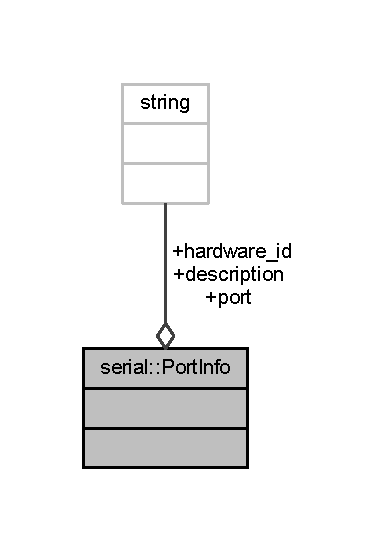
\includegraphics[width=181pt]{structserial_1_1_port_info__coll__graph}
\end{center}
\end{figure}
\subsection*{Public Attributes}
\begin{DoxyCompactItemize}
\item 
std\+::string \mbox{\hyperlink{structserial_1_1_port_info_a5d4242cdd6c0d01260e24964af4c23d2}{port}}
\item 
std\+::string \mbox{\hyperlink{structserial_1_1_port_info_a2ba37dd33d47b554aef5c15c1fe8b872}{description}}
\item 
std\+::string \mbox{\hyperlink{structserial_1_1_port_info_a7d55368e1a4e6ccc9da6f4d339524837}{hardware\+\_\+id}}
\end{DoxyCompactItemize}


\subsection{Detailed Description}
Structure that describes a serial device. 

\subsection{Member Data Documentation}
\mbox{\Hypertarget{structserial_1_1_port_info_a2ba37dd33d47b554aef5c15c1fe8b872}\label{structserial_1_1_port_info_a2ba37dd33d47b554aef5c15c1fe8b872}} 
\index{serial\+::\+Port\+Info@{serial\+::\+Port\+Info}!description@{description}}
\index{description@{description}!serial\+::\+Port\+Info@{serial\+::\+Port\+Info}}
\subsubsection{\texorpdfstring{description}{description}}
{\footnotesize\ttfamily std\+::string serial\+::\+Port\+Info\+::description}

Human readable description of serial device if available. \mbox{\Hypertarget{structserial_1_1_port_info_a7d55368e1a4e6ccc9da6f4d339524837}\label{structserial_1_1_port_info_a7d55368e1a4e6ccc9da6f4d339524837}} 
\index{serial\+::\+Port\+Info@{serial\+::\+Port\+Info}!hardware\+\_\+id@{hardware\+\_\+id}}
\index{hardware\+\_\+id@{hardware\+\_\+id}!serial\+::\+Port\+Info@{serial\+::\+Port\+Info}}
\subsubsection{\texorpdfstring{hardware\+\_\+id}{hardware\_id}}
{\footnotesize\ttfamily std\+::string serial\+::\+Port\+Info\+::hardware\+\_\+id}

Hardware ID (e.\+g. V\+ID\+:P\+ID of U\+SB serial devices) or \char`\"{}n/a\char`\"{} if not available. \mbox{\Hypertarget{structserial_1_1_port_info_a5d4242cdd6c0d01260e24964af4c23d2}\label{structserial_1_1_port_info_a5d4242cdd6c0d01260e24964af4c23d2}} 
\index{serial\+::\+Port\+Info@{serial\+::\+Port\+Info}!port@{port}}
\index{port@{port}!serial\+::\+Port\+Info@{serial\+::\+Port\+Info}}
\subsubsection{\texorpdfstring{port}{port}}
{\footnotesize\ttfamily std\+::string serial\+::\+Port\+Info\+::port}

Address of the serial port (this can be passed to the constructor of \mbox{\hyperlink{classserial_1_1_serial}{Serial}}). 

The documentation for this struct was generated from the following file\+:\begin{DoxyCompactItemize}
\item 
C\+:/folders/d/scripts/cpp/\+O\+P\+T3101\+S\+D\+K/\+O\+P\+T3101\+S\+D\+K/\+O\+P\+T3101\+S\+D\+K/serial\+Lib/\mbox{\hyperlink{serial_8h}{serial.\+h}}\end{DoxyCompactItemize}

\hypertarget{classserial_1_1_port_not_opened_exception}{}\section{serial\+:\+:Port\+Not\+Opened\+Exception Class Reference}
\label{classserial_1_1_port_not_opened_exception}\index{serial\+::\+Port\+Not\+Opened\+Exception@{serial\+::\+Port\+Not\+Opened\+Exception}}


{\ttfamily \#include $<$serial.\+h$>$}



Inheritance diagram for serial\+:\+:Port\+Not\+Opened\+Exception\+:\nopagebreak
\begin{figure}[H]
\begin{center}
\leavevmode
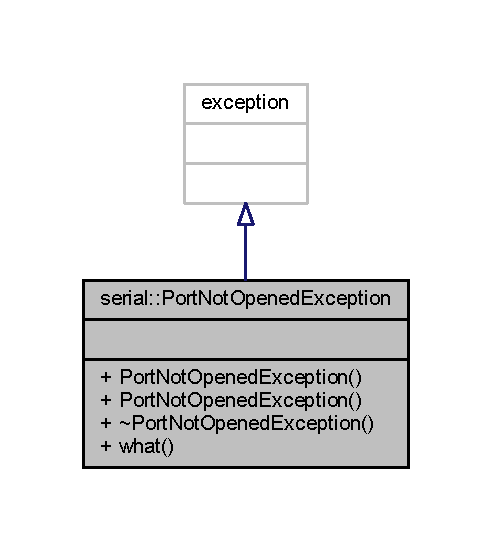
\includegraphics[width=236pt]{classserial_1_1_port_not_opened_exception__inherit__graph}
\end{center}
\end{figure}


Collaboration diagram for serial\+:\+:Port\+Not\+Opened\+Exception\+:\nopagebreak
\begin{figure}[H]
\begin{center}
\leavevmode
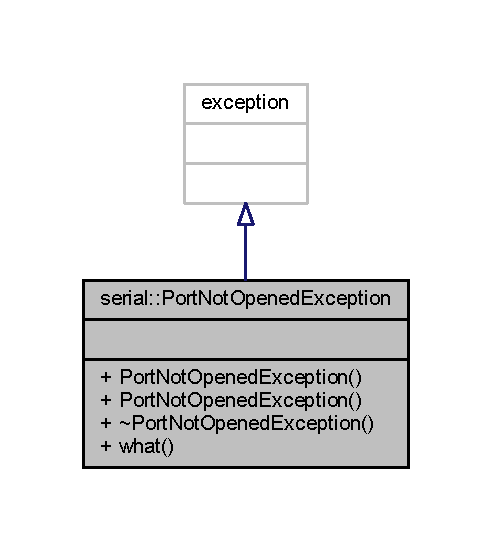
\includegraphics[width=236pt]{classserial_1_1_port_not_opened_exception__coll__graph}
\end{center}
\end{figure}
\subsection*{Public Member Functions}
\begin{DoxyCompactItemize}
\item 
\mbox{\hyperlink{classserial_1_1_port_not_opened_exception_acd2213fae864534eae6a580f74c5ab1b}{Port\+Not\+Opened\+Exception}} (const char $\ast$description)
\item 
\mbox{\hyperlink{classserial_1_1_port_not_opened_exception_ae8b466d10d496a53ed8e9f949e9e628c}{Port\+Not\+Opened\+Exception}} (const \mbox{\hyperlink{classserial_1_1_port_not_opened_exception}{Port\+Not\+Opened\+Exception}} \&other)
\item 
virtual \mbox{\hyperlink{classserial_1_1_port_not_opened_exception_a1d7499214c9f43ed89676f2c90dd72a6}{$\sim$\+Port\+Not\+Opened\+Exception}} ()  throw ()
\item 
virtual const char $\ast$ \mbox{\hyperlink{classserial_1_1_port_not_opened_exception_a002185fbbe0064ebf37038696fa1664d}{what}} () const  throw ()
\end{DoxyCompactItemize}


\subsection{Constructor \& Destructor Documentation}
\mbox{\Hypertarget{classserial_1_1_port_not_opened_exception_acd2213fae864534eae6a580f74c5ab1b}\label{classserial_1_1_port_not_opened_exception_acd2213fae864534eae6a580f74c5ab1b}} 
\index{serial\+::\+Port\+Not\+Opened\+Exception@{serial\+::\+Port\+Not\+Opened\+Exception}!Port\+Not\+Opened\+Exception@{Port\+Not\+Opened\+Exception}}
\index{Port\+Not\+Opened\+Exception@{Port\+Not\+Opened\+Exception}!serial\+::\+Port\+Not\+Opened\+Exception@{serial\+::\+Port\+Not\+Opened\+Exception}}
\subsubsection{\texorpdfstring{Port\+Not\+Opened\+Exception()}{PortNotOpenedException()}\hspace{0.1cm}{\footnotesize\ttfamily [1/2]}}
{\footnotesize\ttfamily serial\+::\+Port\+Not\+Opened\+Exception\+::\+Port\+Not\+Opened\+Exception (\begin{DoxyParamCaption}\item[{const char $\ast$}]{description }\end{DoxyParamCaption})\hspace{0.3cm}{\ttfamily [inline]}}

\mbox{\Hypertarget{classserial_1_1_port_not_opened_exception_ae8b466d10d496a53ed8e9f949e9e628c}\label{classserial_1_1_port_not_opened_exception_ae8b466d10d496a53ed8e9f949e9e628c}} 
\index{serial\+::\+Port\+Not\+Opened\+Exception@{serial\+::\+Port\+Not\+Opened\+Exception}!Port\+Not\+Opened\+Exception@{Port\+Not\+Opened\+Exception}}
\index{Port\+Not\+Opened\+Exception@{Port\+Not\+Opened\+Exception}!serial\+::\+Port\+Not\+Opened\+Exception@{serial\+::\+Port\+Not\+Opened\+Exception}}
\subsubsection{\texorpdfstring{Port\+Not\+Opened\+Exception()}{PortNotOpenedException()}\hspace{0.1cm}{\footnotesize\ttfamily [2/2]}}
{\footnotesize\ttfamily serial\+::\+Port\+Not\+Opened\+Exception\+::\+Port\+Not\+Opened\+Exception (\begin{DoxyParamCaption}\item[{const \mbox{\hyperlink{classserial_1_1_port_not_opened_exception}{Port\+Not\+Opened\+Exception}} \&}]{other }\end{DoxyParamCaption})\hspace{0.3cm}{\ttfamily [inline]}}

\mbox{\Hypertarget{classserial_1_1_port_not_opened_exception_a1d7499214c9f43ed89676f2c90dd72a6}\label{classserial_1_1_port_not_opened_exception_a1d7499214c9f43ed89676f2c90dd72a6}} 
\index{serial\+::\+Port\+Not\+Opened\+Exception@{serial\+::\+Port\+Not\+Opened\+Exception}!````~Port\+Not\+Opened\+Exception@{$\sim$\+Port\+Not\+Opened\+Exception}}
\index{````~Port\+Not\+Opened\+Exception@{$\sim$\+Port\+Not\+Opened\+Exception}!serial\+::\+Port\+Not\+Opened\+Exception@{serial\+::\+Port\+Not\+Opened\+Exception}}
\subsubsection{\texorpdfstring{$\sim$\+Port\+Not\+Opened\+Exception()}{~PortNotOpenedException()}}
{\footnotesize\ttfamily virtual serial\+::\+Port\+Not\+Opened\+Exception\+::$\sim$\+Port\+Not\+Opened\+Exception (\begin{DoxyParamCaption}{ }\end{DoxyParamCaption}) throw  ) \hspace{0.3cm}{\ttfamily [inline]}, {\ttfamily [virtual]}}



\subsection{Member Function Documentation}
\mbox{\Hypertarget{classserial_1_1_port_not_opened_exception_a002185fbbe0064ebf37038696fa1664d}\label{classserial_1_1_port_not_opened_exception_a002185fbbe0064ebf37038696fa1664d}} 
\index{serial\+::\+Port\+Not\+Opened\+Exception@{serial\+::\+Port\+Not\+Opened\+Exception}!what@{what}}
\index{what@{what}!serial\+::\+Port\+Not\+Opened\+Exception@{serial\+::\+Port\+Not\+Opened\+Exception}}
\subsubsection{\texorpdfstring{what()}{what()}}
{\footnotesize\ttfamily virtual const char$\ast$ serial\+::\+Port\+Not\+Opened\+Exception\+::what (\begin{DoxyParamCaption}{ }\end{DoxyParamCaption}) const throw  ) \hspace{0.3cm}{\ttfamily [inline]}, {\ttfamily [virtual]}}



The documentation for this class was generated from the following file\+:\begin{DoxyCompactItemize}
\item 
C\+:/folders/d/scripts/cpp/\+O\+P\+T3101\+S\+D\+K/\+O\+P\+T3101\+S\+D\+K/\+O\+P\+T3101\+S\+D\+K/serial\+Lib/\mbox{\hyperlink{serial_8h}{serial.\+h}}\end{DoxyCompactItemize}

\hypertarget{class_o_p_t3101_1_1registers}{}\section{O\+P\+T3101\+:\+:registers Class Reference}
\label{class_o_p_t3101_1_1registers}\index{O\+P\+T3101\+::registers@{O\+P\+T3101\+::registers}}


Class that enumerates all registers in \mbox{\hyperlink{namespace_o_p_t3101}{O\+P\+T3101}}.  




{\ttfamily \#include $<$O\+P\+T3101\+Register\+Definition.\+h$>$}



Collaboration diagram for O\+P\+T3101\+:\+:registers\+:\nopagebreak
\begin{figure}[H]
\begin{center}
\leavevmode
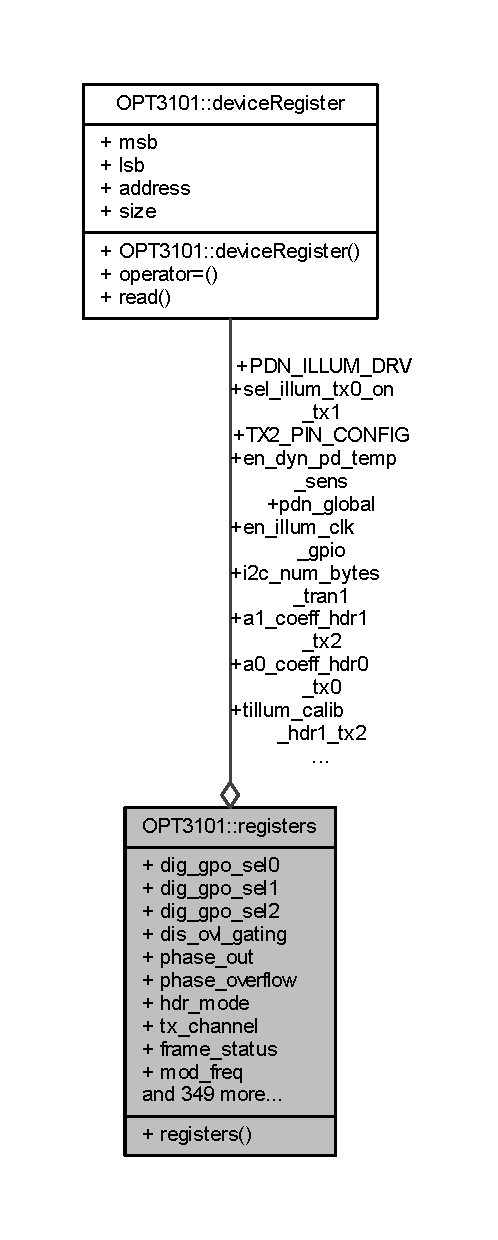
\includegraphics[height=550pt]{class_o_p_t3101_1_1registers__coll__graph}
\end{center}
\end{figure}
\subsection*{Public Member Functions}
\begin{DoxyCompactItemize}
\item 
\mbox{\hyperlink{class_o_p_t3101_1_1registers_ad17b048a9eb5a74b3fef29fb145a9e92}{registers}} ()
\begin{DoxyCompactList}\small\item\em Constructor for class \mbox{\hyperlink{class_o_p_t3101_1_1registers}{O\+P\+T3101\+::registers}} Constructor allocates \mbox{\hyperlink{class_o_p_t3101_1_1device_register_a058d48b4c23e22739b1c65d85367a0a8}{O\+P\+T3101\+::device\+Register\+::size}} to each \mbox{\hyperlink{class_o_p_t3101_1_1device_register}{O\+P\+T3101\+::device\+Register}} instance on construction. \end{DoxyCompactList}\end{DoxyCompactItemize}
\subsection*{Public Attributes}
\begin{DoxyCompactItemize}
\item 
\mbox{\hyperlink{class_o_p_t3101_1_1device_register}{O\+P\+T3101\+::device\+Register}} \mbox{\hyperlink{class_o_p_t3101_1_1registers_a524961a20bb991dfedd371ad04106acb}{dig\+\_\+gpo\+\_\+sel0}}
\begin{DoxyCompactList}\small\item\em dig\+\_\+gpo\+\_\+sel0;Register Addresses\+: 11\mbox{[}3\+:0\mbox{]}; \end{DoxyCompactList}\item 
\mbox{\hyperlink{class_o_p_t3101_1_1device_register}{O\+P\+T3101\+::device\+Register}} \mbox{\hyperlink{class_o_p_t3101_1_1registers_aa4838268aa3b89fbd6e03d9f132072bb}{dig\+\_\+gpo\+\_\+sel1}}
\begin{DoxyCompactList}\small\item\em dig\+\_\+gpo\+\_\+sel1;Register Addresses\+: 11\mbox{[}7\+:4\mbox{]}; \end{DoxyCompactList}\item 
\mbox{\hyperlink{class_o_p_t3101_1_1device_register}{O\+P\+T3101\+::device\+Register}} \mbox{\hyperlink{class_o_p_t3101_1_1registers_a2274058727c99614f1eccf195ddccd6d}{dig\+\_\+gpo\+\_\+sel2}}
\begin{DoxyCompactList}\small\item\em dig\+\_\+gpo\+\_\+sel2;Register Addresses\+: 11\mbox{[}13\+:10\mbox{]}; \end{DoxyCompactList}\item 
\mbox{\hyperlink{class_o_p_t3101_1_1device_register}{O\+P\+T3101\+::device\+Register}} \mbox{\hyperlink{class_o_p_t3101_1_1registers_a258c4f416a6c31685b3e66f1d75921e7}{dis\+\_\+ovl\+\_\+gating}}
\begin{DoxyCompactList}\small\item\em dis\+\_\+ovl\+\_\+gating;Register Addresses\+: 17\mbox{[}15\+:15\mbox{]}; \end{DoxyCompactList}\item 
\mbox{\hyperlink{class_o_p_t3101_1_1device_register}{O\+P\+T3101\+::device\+Register}} \mbox{\hyperlink{class_o_p_t3101_1_1registers_a0b410cb503df506724a4b6a1da49ce1e}{phase\+\_\+out}}
\begin{DoxyCompactList}\small\item\em phase\+\_\+out;Register Addresses\+: 8\mbox{[}15\+:0\mbox{]}; \end{DoxyCompactList}\item 
\mbox{\hyperlink{class_o_p_t3101_1_1device_register}{O\+P\+T3101\+::device\+Register}} \mbox{\hyperlink{class_o_p_t3101_1_1registers_a8d491306e0b4b6e323b09ee8d1c59016}{phase\+\_\+overflow}}
\begin{DoxyCompactList}\small\item\em phase\+\_\+overflow;Register Addresses\+: 8\mbox{[}16\+:16\mbox{]}; \end{DoxyCompactList}\item 
\mbox{\hyperlink{class_o_p_t3101_1_1device_register}{O\+P\+T3101\+::device\+Register}} \mbox{\hyperlink{class_o_p_t3101_1_1registers_a78e8bc6ad4a84c7d19974ba6c58e329e}{hdr\+\_\+mode}}
\begin{DoxyCompactList}\small\item\em hdr\+\_\+mode;Register Addresses\+: 8\mbox{[}17\+:17\mbox{]}; \end{DoxyCompactList}\item 
\mbox{\hyperlink{class_o_p_t3101_1_1device_register}{O\+P\+T3101\+::device\+Register}} \mbox{\hyperlink{class_o_p_t3101_1_1registers_a53518f25f00a5926fda5f0d37ad82fcb}{tx\+\_\+channel}}
\begin{DoxyCompactList}\small\item\em tx\+\_\+channel;Register Addresses\+: 8\mbox{[}19\+:18\mbox{]}; \end{DoxyCompactList}\item 
\mbox{\hyperlink{class_o_p_t3101_1_1device_register}{O\+P\+T3101\+::device\+Register}} \mbox{\hyperlink{class_o_p_t3101_1_1registers_ab8c08b83252a06c3c59b4b33b4b1a8ba}{frame\+\_\+status}}
\begin{DoxyCompactList}\small\item\em frame\+\_\+status;Register Addresses\+: 8\mbox{[}20\+:20\mbox{]}; \end{DoxyCompactList}\item 
\mbox{\hyperlink{class_o_p_t3101_1_1device_register}{O\+P\+T3101\+::device\+Register}} \mbox{\hyperlink{class_o_p_t3101_1_1registers_ad0a150fb8c5e1efeae026e76f2bdbc1f}{mod\+\_\+freq}}
\begin{DoxyCompactList}\small\item\em mod\+\_\+freq;Register Addresses\+: 8\mbox{[}21\+:21\mbox{]}; \end{DoxyCompactList}\item 
\mbox{\hyperlink{class_o_p_t3101_1_1device_register}{O\+P\+T3101\+::device\+Register}} \mbox{\hyperlink{class_o_p_t3101_1_1registers_a93e937bf8d82f09a6024dd226118ef51}{frame\+\_\+count0}}
\begin{DoxyCompactList}\small\item\em frame\+\_\+count0;Register Addresses\+: 8\mbox{[}23\+:23\mbox{]}; \end{DoxyCompactList}\item 
\mbox{\hyperlink{class_o_p_t3101_1_1device_register}{O\+P\+T3101\+::device\+Register}} \mbox{\hyperlink{class_o_p_t3101_1_1registers_a09663efd977de72bdf7820e0a8f92390}{amp\+\_\+out}}
\begin{DoxyCompactList}\small\item\em amp\+\_\+out;Register Addresses\+: 9\mbox{[}15\+:0\mbox{]}; \end{DoxyCompactList}\item 
\mbox{\hyperlink{class_o_p_t3101_1_1device_register}{O\+P\+T3101\+::device\+Register}} \mbox{\hyperlink{class_o_p_t3101_1_1registers_a736858f4b79f2dd5444fc1938148d438}{frame\+\_\+count1}}
\begin{DoxyCompactList}\small\item\em frame\+\_\+count1;Register Addresses\+: 9\mbox{[}17\+:16\mbox{]}; \end{DoxyCompactList}\item 
\mbox{\hyperlink{class_o_p_t3101_1_1device_register}{O\+P\+T3101\+::device\+Register}} \mbox{\hyperlink{class_o_p_t3101_1_1registers_ad767a496a0cad5741d575a54a095add3}{sig\+\_\+ovl\+\_\+flag}}
\begin{DoxyCompactList}\small\item\em sig\+\_\+ovl\+\_\+flag;Register Addresses\+: 9\mbox{[}18\+:18\mbox{]}; \end{DoxyCompactList}\item 
\mbox{\hyperlink{class_o_p_t3101_1_1device_register}{O\+P\+T3101\+::device\+Register}} \mbox{\hyperlink{class_o_p_t3101_1_1registers_a1faab11698859e9d42e148c1d8cd5d1e}{dealias\+\_\+bin}}
\begin{DoxyCompactList}\small\item\em dealias\+\_\+bin;Register Addresses\+: 9\mbox{[}23\+:20\mbox{]}; \end{DoxyCompactList}\item 
\mbox{\hyperlink{class_o_p_t3101_1_1device_register}{O\+P\+T3101\+::device\+Register}} \mbox{\hyperlink{class_o_p_t3101_1_1registers_a1247368fca5573a9ab4b69d541c53a57}{frame\+\_\+count2}}
\begin{DoxyCompactList}\small\item\em frame\+\_\+count2;Register Addresses\+: 10\mbox{[}1\+:0\mbox{]}; \end{DoxyCompactList}\item 
\mbox{\hyperlink{class_o_p_t3101_1_1device_register}{O\+P\+T3101\+::device\+Register}} \mbox{\hyperlink{class_o_p_t3101_1_1registers_ae6b7c86e96cbfb1efe3263caed9de137}{amb\+\_\+data}}
\begin{DoxyCompactList}\small\item\em amb\+\_\+data;Register Addresses\+: 10\mbox{[}11\+:2\mbox{]}; \end{DoxyCompactList}\item 
\mbox{\hyperlink{class_o_p_t3101_1_1device_register}{O\+P\+T3101\+::device\+Register}} \mbox{\hyperlink{class_o_p_t3101_1_1registers_a3dfd8d81d4cb04d274007deb7c6122fc}{tmain}}
\begin{DoxyCompactList}\small\item\em tmain;Register Addresses\+: 10\mbox{[}23\+:12\mbox{]}; \end{DoxyCompactList}\item 
\mbox{\hyperlink{class_o_p_t3101_1_1device_register}{O\+P\+T3101\+::device\+Register}} \mbox{\hyperlink{class_o_p_t3101_1_1registers_abdb9db1e1ff8bda71eccaea718b116d0}{amplitude\+\_\+min\+\_\+thr}}
\begin{DoxyCompactList}\small\item\em amplitude\+\_\+min\+\_\+thr;Register Addresses\+: 16\mbox{[}23\+:16\mbox{]}, 17\mbox{[}23\+:16\mbox{]}; \end{DoxyCompactList}\item 
\mbox{\hyperlink{class_o_p_t3101_1_1device_register}{O\+P\+T3101\+::device\+Register}} \mbox{\hyperlink{class_o_p_t3101_1_1registers_a5ba6f5ef459327f64179b6d405dbd101}{amb\+\_\+ovl\+\_\+flag}}
\begin{DoxyCompactList}\small\item\em amb\+\_\+ovl\+\_\+flag;Register Addresses\+: 8\mbox{[}22\+:22\mbox{]}; \end{DoxyCompactList}\item 
\mbox{\hyperlink{class_o_p_t3101_1_1device_register}{O\+P\+T3101\+::device\+Register}} \mbox{\hyperlink{class_o_p_t3101_1_1registers_a63560e719cf9970bc83879a353b2dc9f}{phase\+\_\+overflow\+\_\+f2}}
\begin{DoxyCompactList}\small\item\em phase\+\_\+overflow\+\_\+f2;Register Addresses\+: 9\mbox{[}19\+:19\mbox{]}; \end{DoxyCompactList}\item 
\mbox{\hyperlink{class_o_p_t3101_1_1device_register}{O\+P\+T3101\+::device\+Register}} \mbox{\hyperlink{class_o_p_t3101_1_1registers_ac5c1fc72abe6fdd9a55ad01fd8116fd3}{ref\+\_\+count\+\_\+limit}}
\begin{DoxyCompactList}\small\item\em ref\+\_\+count\+\_\+limit;Register Addresses\+: 15\mbox{[}14\+:0\mbox{]};this sets the limit of ref-\/clock count when meth1 is used. By programming this we no longer require frequencies which are multiples of powers of 2.;;The default is calculated for 32.\+768 Khz. \end{DoxyCompactList}\item 
\mbox{\hyperlink{class_o_p_t3101_1_1device_register}{O\+P\+T3101\+::device\+Register}} \mbox{\hyperlink{class_o_p_t3101_1_1registers_a50515c2538c13c51a62485ee689c5e1c}{start\+\_\+freq\+\_\+calib}}
\begin{DoxyCompactList}\small\item\em start\+\_\+freq\+\_\+calib;Register Addresses\+: 15\mbox{[}16\+:16\mbox{]};starts the freq\+\_\+calib \end{DoxyCompactList}\item 
\mbox{\hyperlink{class_o_p_t3101_1_1device_register}{O\+P\+T3101\+::device\+Register}} \mbox{\hyperlink{class_o_p_t3101_1_1registers_af4ee9a8bd2c03f0045edee01b1a568ac}{sys\+\_\+clk\+\_\+divider}}
\begin{DoxyCompactList}\small\item\em sys\+\_\+clk\+\_\+divider;Register Addresses\+: 15\mbox{[}20\+:17\mbox{]};The divider can be set according to the ratio b/w ref\+\_\+clk and tg\+\_\+clk. The default is 2 which means default ref\+\_\+clk is assumed at 10 Mhz. ie 40\+Mhz/4 \end{DoxyCompactList}\item 
\mbox{\hyperlink{class_o_p_t3101_1_1device_register}{O\+P\+T3101\+::device\+Register}} \mbox{\hyperlink{class_o_p_t3101_1_1registers_a0d343738560c0bc418f34b458735a811}{freq\+\_\+count\+\_\+read\+\_\+reg}}
\begin{DoxyCompactList}\small\item\em freq\+\_\+count\+\_\+read\+\_\+reg;Register Addresses\+: 16\mbox{[}14\+:0\mbox{]};read register which holds the value of freq\+\_\+loop. \end{DoxyCompactList}\item 
\mbox{\hyperlink{class_o_p_t3101_1_1device_register}{O\+P\+T3101\+::device\+Register}} \mbox{\hyperlink{class_o_p_t3101_1_1registers_a6b28826c31906dc3a27f33b015c4c4d8}{freq\+\_\+count\+\_\+reg}}
\begin{DoxyCompactList}\small\item\em freq\+\_\+count\+\_\+reg;Register Addresses\+: 17\mbox{[}14\+:0\mbox{]};The register which is used for frequency correction when enable\+\_\+auto\+\_\+freq\+\_\+count = \textquotesingle{}0\textquotesingle{} \end{DoxyCompactList}\item 
\mbox{\hyperlink{class_o_p_t3101_1_1device_register}{O\+P\+T3101\+::device\+Register}} \mbox{\hyperlink{class_o_p_t3101_1_1registers_a1c8bf1bb8f6d672bf780e5f99698959d}{en\+\_\+auto\+\_\+freq\+\_\+count}}
\begin{DoxyCompactList}\small\item\em en\+\_\+auto\+\_\+freq\+\_\+count;Register Addresses\+: 15\mbox{[}21\+:21\mbox{]};When this is \textquotesingle{}1\textquotesingle{} internally computed values is used. Else register value is used. \end{DoxyCompactList}\item 
\mbox{\hyperlink{class_o_p_t3101_1_1device_register}{O\+P\+T3101\+::device\+Register}} \mbox{\hyperlink{class_o_p_t3101_1_1registers_acac402a36d4a6b3e8447cbfea307f46e}{en\+\_\+floop}}
\begin{DoxyCompactList}\small\item\em en\+\_\+floop;Register Addresses\+: 15\mbox{[}22\+:22\mbox{]};Enables the freq\+\_\+loop block. If this is \textquotesingle{}0\textquotesingle{}, the clock to the freq\+\_\+loop is gated. \end{DoxyCompactList}\item 
\mbox{\hyperlink{class_o_p_t3101_1_1device_register}{O\+P\+T3101\+::device\+Register}} \mbox{\hyperlink{class_o_p_t3101_1_1registers_a7d1b46e26e943ba29294904855c83871}{en\+\_\+freq\+\_\+corr}}
\begin{DoxyCompactList}\small\item\em en\+\_\+freq\+\_\+corr;Register Addresses\+: 15\mbox{[}23\+:23\mbox{]};This bit applies frequency correction on the phase data either from register or auto\+\_\+freq. \end{DoxyCompactList}\item 
\mbox{\hyperlink{class_o_p_t3101_1_1device_register}{O\+P\+T3101\+::device\+Register}} \mbox{\hyperlink{class_o_p_t3101_1_1registers_aa138ff880edecfdc53ef83bf2cc0dcb8}{en\+\_\+cont\+\_\+fcalib}}
\begin{DoxyCompactList}\small\item\em en\+\_\+cont\+\_\+fcalib;Register Addresses\+: 16\mbox{[}15\+:15\mbox{]}; \end{DoxyCompactList}\item 
\mbox{\hyperlink{class_o_p_t3101_1_1device_register}{O\+P\+T3101\+::device\+Register}} \mbox{\hyperlink{class_o_p_t3101_1_1registers_a158b270484e2829a304f13e30dec3390}{monoshot\+\_\+bit}}
\begin{DoxyCompactList}\small\item\em monoshot\+\_\+bit;Register Addresses\+: 0\mbox{[}23\+:23\mbox{]};In monoshot mode the register to trigger a measurement. \end{DoxyCompactList}\item 
\mbox{\hyperlink{class_o_p_t3101_1_1device_register}{O\+P\+T3101\+::device\+Register}} \mbox{\hyperlink{class_o_p_t3101_1_1registers_adb2df2fa5f4a83807458958db5ee71eb}{monoshot\+\_\+mode}}
\begin{DoxyCompactList}\small\item\em monoshot\+\_\+mode;Register Addresses\+: 39\mbox{[}1\+:0\mbox{]};L\+SB\+: Enters monoshot mode.;;M\+SB\+: If this is set monoshot mode shutdown the oscclk. This has to be used together with monoshot\+\_\+mode. \end{DoxyCompactList}\item 
\mbox{\hyperlink{class_o_p_t3101_1_1device_register}{O\+P\+T3101\+::device\+Register}} \mbox{\hyperlink{class_o_p_t3101_1_1registers_ad70826caf46b032bda2867212f4d2195}{powerup\+\_\+delay}}
\begin{DoxyCompactList}\small\item\em powerup\+\_\+delay;Register Addresses\+: 38\mbox{[}23\+:10\mbox{]};The synchronous counter delay after the ripple counter expires before ungating the clock. About 256$\ast$25ns$\ast$2$^\wedge$6 $\sim$ 400 us. \end{DoxyCompactList}\item 
\mbox{\hyperlink{class_o_p_t3101_1_1device_register}{O\+P\+T3101\+::device\+Register}} \mbox{\hyperlink{class_o_p_t3101_1_1registers_a88eb0b748ad9049d7c563196e7518f43}{monoshot\+\_\+numframe}}
\begin{DoxyCompactList}\small\item\em monoshot\+\_\+numframe;Register Addresses\+: 39\mbox{[}7\+:2\mbox{]};The number of frames of TG to be run after a trigger before shutting down the TG. The default is kept as 6 allowing a led cycle. \end{DoxyCompactList}\item 
\mbox{\hyperlink{class_o_p_t3101_1_1device_register}{O\+P\+T3101\+::device\+Register}} \mbox{\hyperlink{class_o_p_t3101_1_1registers_a7e608b657646a90dd8dfdc3dff0047fb}{monoshot\+\_\+fz\+\_\+clkcnt}}
\begin{DoxyCompactList}\small\item\em monoshot\+\_\+fz\+\_\+clkcnt;Register Addresses\+: 39\mbox{[}23\+:8\mbox{]};The pix\+\_\+cnt at which a monoshot operation freezes. By default just freezes 100 cycles before a frame boundary. \end{DoxyCompactList}\item 
\mbox{\hyperlink{class_o_p_t3101_1_1device_register}{O\+P\+T3101\+::device\+Register}} \mbox{\hyperlink{class_o_p_t3101_1_1registers_a6186d62592ab031ce3a996942b739ab7}{en\+\_\+tx\+\_\+switch}}
\begin{DoxyCompactList}\small\item\em en\+\_\+tx\+\_\+switch;Register Addresses\+: 42\mbox{[}0\+:0\mbox{]};Enable switching of led drivers. \end{DoxyCompactList}\item 
\mbox{\hyperlink{class_o_p_t3101_1_1device_register}{O\+P\+T3101\+::device\+Register}} \mbox{\hyperlink{class_o_p_t3101_1_1registers_af79e0b3cfd511e7aa03cf3e55774f0d0}{sel\+\_\+tx\+\_\+ch}}
\begin{DoxyCompactList}\small\item\em sel\+\_\+tx\+\_\+ch;Register Addresses\+: 42\mbox{[}2\+:1\mbox{]};choses the fix\+\_\+reg value when switching is disabled. \end{DoxyCompactList}\item 
\mbox{\hyperlink{class_o_p_t3101_1_1device_register}{O\+P\+T3101\+::device\+Register}} \mbox{\hyperlink{class_o_p_t3101_1_1registers_a6cd0b1e1ec6febc0e4ec775e4c639d4c}{tx\+\_\+seq\+\_\+reg}}
\begin{DoxyCompactList}\small\item\em tx\+\_\+seq\+\_\+reg;Register Addresses\+: 42\mbox{[}14\+:3\mbox{]};Stores the sequence of led switching in this register.;2-\/1-\/0-\/2-\/1-\/0. The sequence will come as 0-\/1-\/2-\/0-\/1-\/2 \end{DoxyCompactList}\item 
\mbox{\hyperlink{class_o_p_t3101_1_1device_register}{O\+P\+T3101\+::device\+Register}} \mbox{\hyperlink{class_o_p_t3101_1_1registers_ab14fd3da3a7aee59227f3a0b2c6ed653}{en\+\_\+adaptive\+\_\+hdr}}
\begin{DoxyCompactList}\small\item\em en\+\_\+adaptive\+\_\+hdr;Register Addresses\+: 42\mbox{[}15\+:15\mbox{]};enable the adaptive hdr. The num\+\_\+avg\+\_\+frame in this case should be programmed one more than the normal case. \end{DoxyCompactList}\item 
\mbox{\hyperlink{class_o_p_t3101_1_1device_register}{O\+P\+T3101\+::device\+Register}} \mbox{\hyperlink{class_o_p_t3101_1_1registers_a1f8f226c3e13479d0dafeb402d35d519}{sel\+\_\+hdr\+\_\+mode}}
\begin{DoxyCompactList}\small\item\em sel\+\_\+hdr\+\_\+mode;Register Addresses\+: 42\mbox{[}16\+:16\mbox{]};choses which current to use when enable\+\_\+adaptive\+\_\+hdr = \textquotesingle{}0\textquotesingle{} \end{DoxyCompactList}\item 
\mbox{\hyperlink{class_o_p_t3101_1_1device_register}{O\+P\+T3101\+::device\+Register}} \mbox{\hyperlink{class_o_p_t3101_1_1registers_a440d873648ba4fe03c3690e18953610d}{hdr\+\_\+thr\+\_\+low}}
\begin{DoxyCompactList}\small\item\em hdr\+\_\+thr\+\_\+low;Register Addresses\+: 44\mbox{[}15\+:0\mbox{]};The low threshold of the hysterisis loop. Equivalent to $\sim$64 confidence. \end{DoxyCompactList}\item 
\mbox{\hyperlink{class_o_p_t3101_1_1device_register}{O\+P\+T3101\+::device\+Register}} \mbox{\hyperlink{class_o_p_t3101_1_1registers_a9f703a5eeb8b45b076487ee38f56c38b}{hdr\+\_\+thr\+\_\+high}}
\begin{DoxyCompactList}\small\item\em hdr\+\_\+thr\+\_\+high;Register Addresses\+: 43\mbox{[}15\+:0\mbox{]};the high threshold of the hyserisis loop. Default equivalent to confidence of 256 in 16 bit level. \end{DoxyCompactList}\item 
\mbox{\hyperlink{class_o_p_t3101_1_1device_register}{O\+P\+T3101\+::device\+Register}} \mbox{\hyperlink{class_o_p_t3101_1_1registers_a16c4b06813716b1a536015e7089c2d22}{illum\+\_\+scale\+\_\+l\+\_\+tx0}}
\begin{DoxyCompactList}\small\item\em illum\+\_\+scale\+\_\+l\+\_\+tx0;Register Addresses\+: 43\mbox{[}18\+:16\mbox{]}; \end{DoxyCompactList}\item 
\mbox{\hyperlink{class_o_p_t3101_1_1device_register}{O\+P\+T3101\+::device\+Register}} \mbox{\hyperlink{class_o_p_t3101_1_1registers_a2bd8d2bb0c66cd151128107e2e7bdd02}{illum\+\_\+dac\+\_\+l\+\_\+tx0}}
\begin{DoxyCompactList}\small\item\em illum\+\_\+dac\+\_\+l\+\_\+tx0;Register Addresses\+: 41\mbox{[}4\+:0\mbox{]}; \end{DoxyCompactList}\item 
\mbox{\hyperlink{class_o_p_t3101_1_1device_register}{O\+P\+T3101\+::device\+Register}} \mbox{\hyperlink{class_o_p_t3101_1_1registers_a779e2ac88dbf024631877a8fe1446e25}{illum\+\_\+scale\+\_\+h\+\_\+tx0}}
\begin{DoxyCompactList}\small\item\em illum\+\_\+scale\+\_\+h\+\_\+tx0;Register Addresses\+: 43\mbox{[}21\+:19\mbox{]}; \end{DoxyCompactList}\item 
\mbox{\hyperlink{class_o_p_t3101_1_1device_register}{O\+P\+T3101\+::device\+Register}} \mbox{\hyperlink{class_o_p_t3101_1_1registers_a527fc5156f3e32d11843aaa7ef921612}{illum\+\_\+dac\+\_\+h\+\_\+tx0}}
\begin{DoxyCompactList}\small\item\em illum\+\_\+dac\+\_\+h\+\_\+tx0;Register Addresses\+: 41\mbox{[}9\+:5\mbox{]}; \end{DoxyCompactList}\item 
\mbox{\hyperlink{class_o_p_t3101_1_1device_register}{O\+P\+T3101\+::device\+Register}} \mbox{\hyperlink{class_o_p_t3101_1_1registers_aebec846336763223336cfe9673dbcda2}{illum\+\_\+scale\+\_\+l\+\_\+tx1}}
\begin{DoxyCompactList}\small\item\em illum\+\_\+scale\+\_\+l\+\_\+tx1;Register Addresses\+: 44\mbox{[}18\+:16\mbox{]}; \end{DoxyCompactList}\item 
\mbox{\hyperlink{class_o_p_t3101_1_1device_register}{O\+P\+T3101\+::device\+Register}} \mbox{\hyperlink{class_o_p_t3101_1_1registers_a4af53c407da5606b0bf597fb0170903b}{illum\+\_\+dac\+\_\+l\+\_\+tx1}}
\begin{DoxyCompactList}\small\item\em illum\+\_\+dac\+\_\+l\+\_\+tx1;Register Addresses\+: 41\mbox{[}14\+:10\mbox{]}; \end{DoxyCompactList}\item 
\mbox{\hyperlink{class_o_p_t3101_1_1device_register}{O\+P\+T3101\+::device\+Register}} \mbox{\hyperlink{class_o_p_t3101_1_1registers_aa21d0ddf413585c860657ced425be15f}{illum\+\_\+scale\+\_\+h\+\_\+tx1}}
\begin{DoxyCompactList}\small\item\em illum\+\_\+scale\+\_\+h\+\_\+tx1;Register Addresses\+: 44\mbox{[}21\+:19\mbox{]}; \end{DoxyCompactList}\item 
\mbox{\hyperlink{class_o_p_t3101_1_1device_register}{O\+P\+T3101\+::device\+Register}} \mbox{\hyperlink{class_o_p_t3101_1_1registers_af05dedee486d16e110ca46de40b41c71}{illum\+\_\+dac\+\_\+h\+\_\+tx1}}
\begin{DoxyCompactList}\small\item\em illum\+\_\+dac\+\_\+h\+\_\+tx1;Register Addresses\+: 41\mbox{[}19\+:15\mbox{]}; \end{DoxyCompactList}\item 
\mbox{\hyperlink{class_o_p_t3101_1_1device_register}{O\+P\+T3101\+::device\+Register}} \mbox{\hyperlink{class_o_p_t3101_1_1registers_aba9220e6abb4a85a6fba2bc848f347ba}{illum\+\_\+scale\+\_\+l\+\_\+tx2}}
\begin{DoxyCompactList}\small\item\em illum\+\_\+scale\+\_\+l\+\_\+tx2;Register Addresses\+: 185\mbox{[}20\+:18\mbox{]}; \end{DoxyCompactList}\item 
\mbox{\hyperlink{class_o_p_t3101_1_1device_register}{O\+P\+T3101\+::device\+Register}} \mbox{\hyperlink{class_o_p_t3101_1_1registers_a51185e0df51d058ec35728a4a067a075}{illum\+\_\+dac\+\_\+l\+\_\+tx2}}
\begin{DoxyCompactList}\small\item\em illum\+\_\+dac\+\_\+l\+\_\+tx2;Register Addresses\+: 41\mbox{[}23\+:20\mbox{]}, 42\mbox{[}23\+:23\mbox{]}; \end{DoxyCompactList}\item 
\mbox{\hyperlink{class_o_p_t3101_1_1device_register}{O\+P\+T3101\+::device\+Register}} \mbox{\hyperlink{class_o_p_t3101_1_1registers_a01e437455fdcf3e98fa2315da38afb48}{illum\+\_\+scale\+\_\+h\+\_\+tx2}}
\begin{DoxyCompactList}\small\item\em illum\+\_\+scale\+\_\+h\+\_\+tx2;Register Addresses\+: 185\mbox{[}23\+:21\mbox{]}; \end{DoxyCompactList}\item 
\mbox{\hyperlink{class_o_p_t3101_1_1device_register}{O\+P\+T3101\+::device\+Register}} \mbox{\hyperlink{class_o_p_t3101_1_1registers_adfe041f139afb2bc8ae662b5e3f4a630}{illum\+\_\+dac\+\_\+h\+\_\+tx2}}
\begin{DoxyCompactList}\small\item\em illum\+\_\+dac\+\_\+h\+\_\+tx2;Register Addresses\+: 42\mbox{[}22\+:18\mbox{]}; \end{DoxyCompactList}\item 
\mbox{\hyperlink{class_o_p_t3101_1_1device_register}{O\+P\+T3101\+::device\+Register}} \mbox{\hyperlink{class_o_p_t3101_1_1registers_a264eda6822d89e022cddb6f1c2217028}{amb\+\_\+adc\+\_\+in\+\_\+tx0}}
\begin{DoxyCompactList}\small\item\em amb\+\_\+adc\+\_\+in\+\_\+tx0;Register Addresses\+: 185\mbox{[}13\+:12\mbox{]}; \end{DoxyCompactList}\item 
\mbox{\hyperlink{class_o_p_t3101_1_1device_register}{O\+P\+T3101\+::device\+Register}} \mbox{\hyperlink{class_o_p_t3101_1_1registers_a6f5ba848c54ce6b47d8364879358c31b}{amb\+\_\+adc\+\_\+in\+\_\+tx1}}
\begin{DoxyCompactList}\small\item\em amb\+\_\+adc\+\_\+in\+\_\+tx1;Register Addresses\+: 185\mbox{[}15\+:14\mbox{]}; \end{DoxyCompactList}\item 
\mbox{\hyperlink{class_o_p_t3101_1_1device_register}{O\+P\+T3101\+::device\+Register}} \mbox{\hyperlink{class_o_p_t3101_1_1registers_a585e9fc419172f85b90262871e40027b}{amb\+\_\+adc\+\_\+in\+\_\+tx2}}
\begin{DoxyCompactList}\small\item\em amb\+\_\+adc\+\_\+in\+\_\+tx2;Register Addresses\+: 185\mbox{[}17\+:16\mbox{]}; \end{DoxyCompactList}\item 
\mbox{\hyperlink{class_o_p_t3101_1_1device_register}{O\+P\+T3101\+::device\+Register}} \mbox{\hyperlink{class_o_p_t3101_1_1registers_a5c5d2db376e2b9808805ab04660503d1}{give\+\_\+dealias\+\_\+data}}
\begin{DoxyCompactList}\small\item\em give\+\_\+dealias\+\_\+data;Register Addresses\+: 184\mbox{[}20\+:20\mbox{]}; \end{DoxyCompactList}\item 
\mbox{\hyperlink{class_o_p_t3101_1_1device_register}{O\+P\+T3101\+::device\+Register}} \mbox{\hyperlink{class_o_p_t3101_1_1registers_a0ada6bc0729541f5740281e93a12cc22}{en\+\_\+dealias\+\_\+meas}}
\begin{DoxyCompactList}\small\item\em en\+\_\+dealias\+\_\+meas;Register Addresses\+: 64\mbox{[}0\+:0\mbox{]};enables dealias calculation.;Normally with enable\+\_\+dealiased\+\_\+measurement set and enable\+\_\+multi\+\_\+freq\+\_\+phase is unset a combined distance and kb is given out. In the normal phase register, phase of the high frequency itself is given.; \end{DoxyCompactList}\item 
\mbox{\hyperlink{class_o_p_t3101_1_1device_register}{O\+P\+T3101\+::device\+Register}} \mbox{\hyperlink{class_o_p_t3101_1_1registers_a6a2fb5089cb59657163752ab2bc8fd0c}{ncr\+\_\+config}}
\begin{DoxyCompactList}\small\item\em ncr\+\_\+config;Register Addresses\+: 64\mbox{[}21\+:21\mbox{]};option to chose ncr configuration, that is 6/7 (0) or 6/5 (1). Chooses higher frequency by default. \end{DoxyCompactList}\item 
\mbox{\hyperlink{class_o_p_t3101_1_1device_register}{O\+P\+T3101\+::device\+Register}} \mbox{\hyperlink{class_o_p_t3101_1_1registers_a29ac388846dfe0bbbdcee909aeb94b04}{alpha0\+\_\+dealias\+\_\+scale}}
\begin{DoxyCompactList}\small\item\em alpha0\+\_\+dealias\+\_\+scale;Register Addresses\+: 64\mbox{[}14\+:9\mbox{]};indicates the vector multiplication in intrinsic-\/xtalk component for the dealias frequency. Default is \textquotesingle{}1\textquotesingle{}. \end{DoxyCompactList}\item 
\mbox{\hyperlink{class_o_p_t3101_1_1device_register}{O\+P\+T3101\+::device\+Register}} \mbox{\hyperlink{class_o_p_t3101_1_1registers_ad825eb1e8381dd0aa83afcc9eef9c4a2}{beta0\+\_\+dealias\+\_\+scale}}
\begin{DoxyCompactList}\small\item\em beta0\+\_\+dealias\+\_\+scale;Register Addresses\+: 64\mbox{[}20\+:15\mbox{]}; \end{DoxyCompactList}\item 
\mbox{\hyperlink{class_o_p_t3101_1_1device_register}{O\+P\+T3101\+::device\+Register}} \mbox{\hyperlink{class_o_p_t3101_1_1registers_a712fda429e950ee47aa365e4b7dfd1a8}{alpha1\+\_\+dealias\+\_\+scale}}
\begin{DoxyCompactList}\small\item\em alpha1\+\_\+dealias\+\_\+scale;Register Addresses\+: 65\mbox{[}5\+:0\mbox{]};indicates the vector multiplication in optical-\/xtalk component for the dealias frequency. Default is \textquotesingle{}1\textquotesingle{}. \end{DoxyCompactList}\item 
\mbox{\hyperlink{class_o_p_t3101_1_1device_register}{O\+P\+T3101\+::device\+Register}} \mbox{\hyperlink{class_o_p_t3101_1_1registers_a6d9fd3f6940ec2d1bc40b6eb672ad333}{beta1\+\_\+dealias\+\_\+scale}}
\begin{DoxyCompactList}\small\item\em beta1\+\_\+dealias\+\_\+scale;Register Addresses\+: 65\mbox{[}11\+:6\mbox{]}; \end{DoxyCompactList}\item 
\mbox{\hyperlink{class_o_p_t3101_1_1device_register}{O\+P\+T3101\+::device\+Register}} \mbox{\hyperlink{class_o_p_t3101_1_1registers_a0d7d9f45b7942f6913a4a57e9481beaf}{en\+\_\+multi\+\_\+freq\+\_\+phase}}
\begin{DoxyCompactList}\small\item\em en\+\_\+multi\+\_\+freq\+\_\+phase;Register Addresses\+: 64\mbox{[}22\+:22\mbox{]};With this bit set along with enable\+\_\+dealiased\+\_\+measurement, the usual phase register will have both the frequency information. The frequency of the phase will be indicated in one of the status bit. \end{DoxyCompactList}\item 
\mbox{\hyperlink{class_o_p_t3101_1_1device_register}{O\+P\+T3101\+::device\+Register}} \mbox{\hyperlink{class_o_p_t3101_1_1registers_a111dc31dd6ec741a97786e5207b7bc7b}{temp\+\_\+avg\+\_\+main}}
\begin{DoxyCompactList}\small\item\em temp\+\_\+avg\+\_\+main;Register Addresses\+: 3\mbox{[}23\+:22\mbox{]}; \end{DoxyCompactList}\item 
\mbox{\hyperlink{class_o_p_t3101_1_1device_register}{O\+P\+T3101\+::device\+Register}} \mbox{\hyperlink{class_o_p_t3101_1_1registers_aadd456d05604771656442bf5f1ff0514}{dis\+\_\+ovl\+\_\+for\+\_\+hdr\+\_\+meth1}}
\begin{DoxyCompactList}\small\item\em dis\+\_\+ovl\+\_\+for\+\_\+hdr\+\_\+meth1;Register Addresses\+: 184\mbox{[}21\+:21\mbox{]}; \end{DoxyCompactList}\item 
\mbox{\hyperlink{class_o_p_t3101_1_1device_register}{O\+P\+T3101\+::device\+Register}} \mbox{\hyperlink{class_o_p_t3101_1_1registers_a3c076b5de6e72eff036b9371c91bfa3e}{en\+\_\+ovl\+\_\+for\+\_\+hdr\+\_\+meth2}}
\begin{DoxyCompactList}\small\item\em en\+\_\+ovl\+\_\+for\+\_\+hdr\+\_\+meth2;Register Addresses\+: 184\mbox{[}22\+:22\mbox{]}; \end{DoxyCompactList}\item 
\mbox{\hyperlink{class_o_p_t3101_1_1device_register}{O\+P\+T3101\+::device\+Register}} \mbox{\hyperlink{class_o_p_t3101_1_1registers_a72ee56b2c4fc0d6b04e2edfbf036f8ec}{en\+\_\+tx1\+\_\+on\+\_\+tx0}}
\begin{DoxyCompactList}\small\item\em en\+\_\+tx1\+\_\+on\+\_\+tx0;Register Addresses\+: 185\mbox{[}10\+:10\mbox{]}; \end{DoxyCompactList}\item 
\mbox{\hyperlink{class_o_p_t3101_1_1device_register}{O\+P\+T3101\+::device\+Register}} \mbox{\hyperlink{class_o_p_t3101_1_1registers_abf81e8f737e0288f11211ecf48e698b7}{en\+\_\+tx2\+\_\+on\+\_\+tx0}}
\begin{DoxyCompactList}\small\item\em en\+\_\+tx2\+\_\+on\+\_\+tx0;Register Addresses\+: 185\mbox{[}11\+:11\mbox{]}; \end{DoxyCompactList}\item 
\mbox{\hyperlink{class_o_p_t3101_1_1device_register}{O\+P\+T3101\+::device\+Register}} \mbox{\hyperlink{class_o_p_t3101_1_1registers_a7f492976fddcfa840372b5e531f7cf86}{clip\+\_\+mode\+\_\+fc}}
\begin{DoxyCompactList}\small\item\em clip\+\_\+mode\+\_\+fc;Register Addresses\+: 80\mbox{[}0\+:0\mbox{]};chooses either rounding off or clipping or wrap around when applying freq-\/correction. Default is kept as rounding. \end{DoxyCompactList}\item 
\mbox{\hyperlink{class_o_p_t3101_1_1device_register}{O\+P\+T3101\+::device\+Register}} \mbox{\hyperlink{class_o_p_t3101_1_1registers_a50e6410737d9b479ceed94b6521b566d}{clip\+\_\+mode\+\_\+nl}}
\begin{DoxyCompactList}\small\item\em clip\+\_\+mode\+\_\+nl;Register Addresses\+: 80\mbox{[}1\+:1\mbox{]};chooses either rounding off or clipping or wrap around when applying harmonic correction. Default is kept as rounding. \end{DoxyCompactList}\item 
\mbox{\hyperlink{class_o_p_t3101_1_1device_register}{O\+P\+T3101\+::device\+Register}} \mbox{\hyperlink{class_o_p_t3101_1_1registers_abe6e94cb9cc2611cca3f47a29447b92c}{clip\+\_\+mode\+\_\+temp}}
\begin{DoxyCompactList}\small\item\em clip\+\_\+mode\+\_\+temp;Register Addresses\+: 80\mbox{[}2\+:2\mbox{]};chooses either rounding off or clipping or wrap around when applying temp correction. Default is kept as rounding. \end{DoxyCompactList}\item 
\mbox{\hyperlink{class_o_p_t3101_1_1device_register}{O\+P\+T3101\+::device\+Register}} \mbox{\hyperlink{class_o_p_t3101_1_1registers_ae4e6e6a2afdbe9aa78d7bef9f0937eb7}{clip\+\_\+mode\+\_\+offset}}
\begin{DoxyCompactList}\small\item\em clip\+\_\+mode\+\_\+offset;Register Addresses\+: 80\mbox{[}3\+:3\mbox{]};chooses either rounding off or clipping or wrap around when applying offset. Default is kept as rounding. \end{DoxyCompactList}\item 
\mbox{\hyperlink{class_o_p_t3101_1_1device_register}{O\+P\+T3101\+::device\+Register}} \mbox{\hyperlink{class_o_p_t3101_1_1registers_ab57b1df98f5f15dd8027331041bfcfa3}{disable\+\_\+syncing}}
\begin{DoxyCompactList}\small\item\em disable\+\_\+syncing;Register Addresses\+: 80\mbox{[}21\+:21\mbox{]};Normally calc clock and afe\+\_\+clk are synchronized to avoid reset to reset variation in spur levels. This option is to disable the syncing of dividers (of calc\+\_\+clk). The default is now changed to \textquotesingle{}1\textquotesingle{} because we don\textquotesingle{}t use divided clock for calc-\/clk from P\+G3\+P0 by default. If syncing is used frequency loop will have issues. \end{DoxyCompactList}\item 
\mbox{\hyperlink{class_o_p_t3101_1_1device_register}{O\+P\+T3101\+::device\+Register}} \mbox{\hyperlink{class_o_p_t3101_1_1registers_a41a1c843f871b218c7ead6c8b4a4aca6}{force\+\_\+en\+\_\+slave}}
\begin{DoxyCompactList}\small\item\em force\+\_\+en\+\_\+slave;Register Addresses\+: 0\mbox{[}22\+:22\mbox{]};Enable i2c slave for any address forcefully. That is whether auto\+\_\+load completed or not. \end{DoxyCompactList}\item 
\mbox{\hyperlink{class_o_p_t3101_1_1device_register}{O\+P\+T3101\+::device\+Register}} \mbox{\hyperlink{class_o_p_t3101_1_1registers_a8ce40d49958ba30cfd4f7072624072e4}{force\+\_\+en\+\_\+bypass}}
\begin{DoxyCompactList}\small\item\em force\+\_\+en\+\_\+bypass;Register Addresses\+: 0\mbox{[}21\+:21\mbox{]};This bit allows the slave to write directly to the efuse. This is gated with stop condition at the port level to avoid transition signals at scl/sda. \end{DoxyCompactList}\item 
\mbox{\hyperlink{class_o_p_t3101_1_1device_register}{O\+P\+T3101\+::device\+Register}} \mbox{\hyperlink{class_o_p_t3101_1_1registers_a74924d92cebb360f0486813366722331}{override\+\_\+clkgen\+\_\+reg}}
\begin{DoxyCompactList}\small\item\em override\+\_\+clkgen\+\_\+reg;Register Addresses\+: 80\mbox{[}22\+:22\mbox{]};Setting this register \textquotesingle{}1\textquotesingle{} allows user to independenly control tm\+\_\+clkgen(2\+:1) which controls dealias settings. \end{DoxyCompactList}\item 
\mbox{\hyperlink{class_o_p_t3101_1_1device_register}{O\+P\+T3101\+::device\+Register}} \mbox{\hyperlink{class_o_p_t3101_1_1registers_a1223651c77a8bcf33f083b0d668f028d}{software\+\_\+reset}}
\begin{DoxyCompactList}\small\item\em software\+\_\+reset;Register Addresses\+: 0\mbox{[}0\+:0\mbox{]}; \end{DoxyCompactList}\item 
\mbox{\hyperlink{class_o_p_t3101_1_1device_register}{O\+P\+T3101\+::device\+Register}} \mbox{\hyperlink{class_o_p_t3101_1_1registers_af37f171c335d8995b3ce666501c18dbe}{dis\+\_\+tg\+\_\+aconf}}
\begin{DoxyCompactList}\small\item\em dis\+\_\+tg\+\_\+aconf;Register Addresses\+: 128\mbox{[}23\+:23\mbox{]};Some of the tg registers are automatically configured such as pdn$\ast$\+\_\+dyn\+\_\+tg signal, capture\+\_\+tg\+\_\+channel etc. if these signals need to be configured by user this bit may be used as an override. \end{DoxyCompactList}\item 
\mbox{\hyperlink{class_o_p_t3101_1_1device_register}{O\+P\+T3101\+::device\+Register}} \mbox{\hyperlink{class_o_p_t3101_1_1registers_a487fb0695a2b670e47f3a5d2a86099fe}{capture\+\_\+clk\+\_\+cnt}}
\begin{DoxyCompactList}\small\item\em capture\+\_\+clk\+\_\+cnt;Register Addresses\+: 160\mbox{[}15\+:0\mbox{]};This is where early\+\_\+fvd/svd starts. early\+\_\+fvd only comes in the frame which is equal num\+\_\+avg. This is the subframe in which computation results comes up. Programm this to 10600 if planning to use lower frequency. \end{DoxyCompactList}\item 
\mbox{\hyperlink{class_o_p_t3101_1_1device_register}{O\+P\+T3101\+::device\+Register}} \mbox{\hyperlink{class_o_p_t3101_1_1registers_a89a7d424e929b98a2ebde2007943a84b}{tg\+\_\+en}}
\begin{DoxyCompactList}\small\item\em tg\+\_\+en;Register Addresses\+: 128\mbox{[}0\+:0\mbox{]};gates the tg\+\_\+clk with this bit. \end{DoxyCompactList}\item 
\mbox{\hyperlink{class_o_p_t3101_1_1device_register}{O\+P\+T3101\+::device\+Register}} \mbox{\hyperlink{class_o_p_t3101_1_1registers_a580fcd93b67fc370744aa6f366a0cf27}{num\+\_\+sub\+\_\+frames}}
\begin{DoxyCompactList}\small\item\em num\+\_\+sub\+\_\+frames;Register Addresses\+: 159\mbox{[}11\+:0\mbox{]};The numbef of subframes in a frame. This number should be greater than or equal to num\+\_\+avg. \end{DoxyCompactList}\item 
\mbox{\hyperlink{class_o_p_t3101_1_1device_register}{O\+P\+T3101\+::device\+Register}} \mbox{\hyperlink{class_o_p_t3101_1_1registers_a9b89956eebb5258cbb968ba07182c98c}{num\+\_\+avg\+\_\+sub\+\_\+frames}}
\begin{DoxyCompactList}\small\item\em num\+\_\+avg\+\_\+sub\+\_\+frames;Register Addresses\+: 159\mbox{[}23\+:12\mbox{]};The number of averages for the iq. Used in TG to generate early\+\_\+fvd and some other TG signals. \end{DoxyCompactList}\item 
\mbox{\hyperlink{class_o_p_t3101_1_1device_register}{O\+P\+T3101\+::device\+Register}} \mbox{\hyperlink{class_o_p_t3101_1_1registers_abc883ba2fcc4156c6e28e3b673de0a1a}{sub\+\_\+vd\+\_\+clk\+\_\+cnt}}
\begin{DoxyCompactList}\small\item\em sub\+\_\+vd\+\_\+clk\+\_\+cnt;Register Addresses\+: 128\mbox{[}16\+:1\mbox{]};the number of pixels in a subframe. In P\+G3\+P0 the default is changed to support 4ksps. The number is also made a multiple of 32+16. \end{DoxyCompactList}\item 
\mbox{\hyperlink{class_o_p_t3101_1_1device_register}{O\+P\+T3101\+::device\+Register}} \mbox{\hyperlink{class_o_p_t3101_1_1registers_adf94f254c8aa46637771a1b01949d680}{tg\+\_\+illumen\+\_\+start}}
\begin{DoxyCompactList}\small\item\em tg\+\_\+illumen\+\_\+start;Register Addresses\+: 143\mbox{[}15\+:0\mbox{]};spare2\+\_\+tg. This is used for illum\+\_\+en. Enabled throughout a subframe. \end{DoxyCompactList}\item 
\mbox{\hyperlink{class_o_p_t3101_1_1device_register}{O\+P\+T3101\+::device\+Register}} \mbox{\hyperlink{class_o_p_t3101_1_1registers_a70082ca9b2affbe66ae355c3f66df5cb}{tg\+\_\+illumen\+\_\+end}}
\begin{DoxyCompactList}\small\item\em tg\+\_\+illumen\+\_\+end;Register Addresses\+: 144\mbox{[}15\+:0\mbox{]};Ending after the 8192+ 250 samples apx. \end{DoxyCompactList}\item 
\mbox{\hyperlink{class_o_p_t3101_1_1device_register}{O\+P\+T3101\+::device\+Register}} \mbox{\hyperlink{class_o_p_t3101_1_1registers_a5cf64985550cfe24cc722d40ab011be5}{tg\+\_\+illumen\+\_\+mask\+\_\+start}}
\begin{DoxyCompactList}\small\item\em tg\+\_\+illumen\+\_\+mask\+\_\+start;Register Addresses\+: 156\mbox{[}11\+:0\mbox{]};spare2\+\_\+mask. By default the mask is programmed till num\+\_\+avg\+\_\+iq only. \end{DoxyCompactList}\item 
\mbox{\hyperlink{class_o_p_t3101_1_1device_register}{O\+P\+T3101\+::device\+Register}} \mbox{\hyperlink{class_o_p_t3101_1_1registers_af45af1b39e7f8d73bece88e66f68de06}{tg\+\_\+illumen\+\_\+mask\+\_\+end}}
\begin{DoxyCompactList}\small\item\em tg\+\_\+illumen\+\_\+mask\+\_\+end;Register Addresses\+: 156\mbox{[}23\+:12\mbox{]}; \end{DoxyCompactList}\item 
\mbox{\hyperlink{class_o_p_t3101_1_1device_register}{O\+P\+T3101\+::device\+Register}} \mbox{\hyperlink{class_o_p_t3101_1_1registers_abe9a28eaeb59586d08377edb39dde6a8}{tg\+\_\+afe\+\_\+rst\+\_\+start}}
\begin{DoxyCompactList}\small\item\em tg\+\_\+afe\+\_\+rst\+\_\+start;Register Addresses\+: 131\mbox{[}15\+:0\mbox{]};demod\+\_\+reset. Mask is programmed such that it comes every subframe. \end{DoxyCompactList}\item 
\mbox{\hyperlink{class_o_p_t3101_1_1device_register}{O\+P\+T3101\+::device\+Register}} \mbox{\hyperlink{class_o_p_t3101_1_1registers_abc508beaa4d4a7284b224406c1c97dee}{tg\+\_\+afe\+\_\+rst\+\_\+end}}
\begin{DoxyCompactList}\small\item\em tg\+\_\+afe\+\_\+rst\+\_\+end;Register Addresses\+: 132\mbox{[}15\+:0\mbox{]}; \end{DoxyCompactList}\item 
\mbox{\hyperlink{class_o_p_t3101_1_1device_register}{O\+P\+T3101\+::device\+Register}} \mbox{\hyperlink{class_o_p_t3101_1_1registers_a0a60b0f7f4db214f884dd21be76e47d1}{tg\+\_\+seq\+\_\+int\+\_\+start}}
\begin{DoxyCompactList}\small\item\em tg\+\_\+seq\+\_\+int\+\_\+start;Register Addresses\+: 133\mbox{[}15\+:0\mbox{]};interrupt. Only happens in first subframe due to the mask programming \end{DoxyCompactList}\item 
\mbox{\hyperlink{class_o_p_t3101_1_1device_register}{O\+P\+T3101\+::device\+Register}} \mbox{\hyperlink{class_o_p_t3101_1_1registers_a5d64a1d13384ed3b40bab6024a15bb75}{tg\+\_\+seq\+\_\+int\+\_\+end}}
\begin{DoxyCompactList}\small\item\em tg\+\_\+seq\+\_\+int\+\_\+end;Register Addresses\+: 134\mbox{[}15\+:0\mbox{]}; \end{DoxyCompactList}\item 
\mbox{\hyperlink{class_o_p_t3101_1_1device_register}{O\+P\+T3101\+::device\+Register}} \mbox{\hyperlink{class_o_p_t3101_1_1registers_a54a3244c947bb01cc57e706cd81ec0e2}{tg\+\_\+capture\+\_\+start}}
\begin{DoxyCompactList}\small\item\em tg\+\_\+capture\+\_\+start;Register Addresses\+: 135\mbox{[}15\+:0\mbox{]};capture\+\_\+tg\+\_\+channel. Internal TG signal. This signal need to be changed when you go to slower dealias mode. Program this to 11300 and 11800 \end{DoxyCompactList}\item 
\mbox{\hyperlink{class_o_p_t3101_1_1device_register}{O\+P\+T3101\+::device\+Register}} \mbox{\hyperlink{class_o_p_t3101_1_1registers_a61bb2d508902da5f6189058aaa7a21d5}{tg\+\_\+capture\+\_\+end}}
\begin{DoxyCompactList}\small\item\em tg\+\_\+capture\+\_\+end;Register Addresses\+: 136\mbox{[}15\+:0\mbox{]}; \end{DoxyCompactList}\item 
\mbox{\hyperlink{class_o_p_t3101_1_1device_register}{O\+P\+T3101\+::device\+Register}} \mbox{\hyperlink{class_o_p_t3101_1_1registers_a0bb0bde768833ea431ed687d71f7b7cf}{tg\+\_\+ovl\+\_\+window\+\_\+start}}
\begin{DoxyCompactList}\small\item\em tg\+\_\+ovl\+\_\+window\+\_\+start;Register Addresses\+: 137\mbox{[}15\+:0\mbox{]};ovl\+\_\+sample. During this time period only ovl is sampled. This exists for only for subframes till the num\+\_\+avg. \end{DoxyCompactList}\item 
\mbox{\hyperlink{class_o_p_t3101_1_1device_register}{O\+P\+T3101\+::device\+Register}} \mbox{\hyperlink{class_o_p_t3101_1_1registers_afde33d8e7e972a532373fabf602af1e2}{tg\+\_\+ovl\+\_\+window\+\_\+end}}
\begin{DoxyCompactList}\small\item\em tg\+\_\+ovl\+\_\+window\+\_\+end;Register Addresses\+: 138\mbox{[}15\+:0\mbox{]}; \end{DoxyCompactList}\item 
\mbox{\hyperlink{class_o_p_t3101_1_1device_register}{O\+P\+T3101\+::device\+Register}} \mbox{\hyperlink{class_o_p_t3101_1_1registers_ab1ac2d988d3463d49c708505b9d10e38}{tg\+\_\+calc\+\_\+start}}
\begin{DoxyCompactList}\small\item\em tg\+\_\+calc\+\_\+start;Register Addresses\+: 145\mbox{[}15\+:0\mbox{]};pdn\+\_\+dyn\+\_\+tg. This signal exists roughly from early\+\_\+fvd start till end of the computation. The mask is programmed such that this only comes in the num\+\_\+avg sub-\/frame. Programmed such that it will work even if the frequency changes in both direction. \end{DoxyCompactList}\item 
\mbox{\hyperlink{class_o_p_t3101_1_1device_register}{O\+P\+T3101\+::device\+Register}} \mbox{\hyperlink{class_o_p_t3101_1_1registers_a853eb6fac21dd74584680fe828477be8}{tg\+\_\+calc\+\_\+end}}
\begin{DoxyCompactList}\small\item\em tg\+\_\+calc\+\_\+end;Register Addresses\+: 146\mbox{[}15\+:0\mbox{]}; \end{DoxyCompactList}\item 
\mbox{\hyperlink{class_o_p_t3101_1_1device_register}{O\+P\+T3101\+::device\+Register}} \mbox{\hyperlink{class_o_p_t3101_1_1registers_a8e552798736ae98ba96bc672fc5f46d4}{tg\+\_\+dynpdn\+\_\+start}}
\begin{DoxyCompactList}\small\item\em tg\+\_\+dynpdn\+\_\+start;Register Addresses\+: 147\mbox{[}15\+:0\mbox{]};pdn\+\_\+dyn1\+\_\+tg. Used to power down less power intensive digital blocks and analog if tm\+\_\+frame\+\_\+vd\+\_\+sub\+\_\+cnt greater than num\+\_\+avg\+\_\+iq. \end{DoxyCompactList}\item 
\mbox{\hyperlink{class_o_p_t3101_1_1device_register}{O\+P\+T3101\+::device\+Register}} \mbox{\hyperlink{class_o_p_t3101_1_1registers_a97c8582f0bd644163e48032cf137ffc2}{tg\+\_\+dynpdn\+\_\+end}}
\begin{DoxyCompactList}\small\item\em tg\+\_\+dynpdn\+\_\+end;Register Addresses\+: 148\mbox{[}15\+:0\mbox{]}; \end{DoxyCompactList}\item 
\mbox{\hyperlink{class_o_p_t3101_1_1device_register}{O\+P\+T3101\+::device\+Register}} \mbox{\hyperlink{class_o_p_t3101_1_1registers_a6a07f581e0aea372246d40ab03ef4b5d}{tg\+\_\+seq\+\_\+int\+\_\+mask\+\_\+start}}
\begin{DoxyCompactList}\small\item\em tg\+\_\+seq\+\_\+int\+\_\+mask\+\_\+start;Register Addresses\+: 151\mbox{[}11\+:0\mbox{]};interrupt. Comes only in first (num\+:0) subframe. \end{DoxyCompactList}\item 
\mbox{\hyperlink{class_o_p_t3101_1_1device_register}{O\+P\+T3101\+::device\+Register}} \mbox{\hyperlink{class_o_p_t3101_1_1registers_a362b1ed95fa8607822bec7117134619c}{tg\+\_\+seq\+\_\+int\+\_\+mask\+\_\+end}}
\begin{DoxyCompactList}\small\item\em tg\+\_\+seq\+\_\+int\+\_\+mask\+\_\+end;Register Addresses\+: 151\mbox{[}23\+:12\mbox{]}; \end{DoxyCompactList}\item 
\mbox{\hyperlink{class_o_p_t3101_1_1device_register}{O\+P\+T3101\+::device\+Register}} \mbox{\hyperlink{class_o_p_t3101_1_1registers_a943365fa49060742fa49602a1700821c}{tg\+\_\+capture\+\_\+mask\+\_\+start}}
\begin{DoxyCompactList}\small\item\em tg\+\_\+capture\+\_\+mask\+\_\+start;Register Addresses\+: 152\mbox{[}11\+:0\mbox{]};capture\+\_\+tg\+\_\+channel. By default comes only in the num\+\_\+avg subchannel. This mask is configurable by user only if dis\+\_\+tg\+\_\+aconf = \textquotesingle{}1\textquotesingle{}. \end{DoxyCompactList}\item 
\mbox{\hyperlink{class_o_p_t3101_1_1device_register}{O\+P\+T3101\+::device\+Register}} \mbox{\hyperlink{class_o_p_t3101_1_1registers_ade793e58a1728490c89346e2ecaf2914}{tg\+\_\+capture\+\_\+mask\+\_\+end}}
\begin{DoxyCompactList}\small\item\em tg\+\_\+capture\+\_\+mask\+\_\+end;Register Addresses\+: 152\mbox{[}23\+:12\mbox{]}; \end{DoxyCompactList}\item 
\mbox{\hyperlink{class_o_p_t3101_1_1device_register}{O\+P\+T3101\+::device\+Register}} \mbox{\hyperlink{class_o_p_t3101_1_1registers_a990dca0856bffa9f6b8050a0630583bc}{tg\+\_\+ovl\+\_\+window\+\_\+mask\+\_\+start}}
\begin{DoxyCompactList}\small\item\em tg\+\_\+ovl\+\_\+window\+\_\+mask\+\_\+start;Register Addresses\+: 153\mbox{[}11\+:0\mbox{]};ovl\+\_\+sample. This exits till num\+\_\+avg subframe. \end{DoxyCompactList}\item 
\mbox{\hyperlink{class_o_p_t3101_1_1device_register}{O\+P\+T3101\+::device\+Register}} \mbox{\hyperlink{class_o_p_t3101_1_1registers_aec4f1ad9cea554d2ab16e0808ac25b49}{tg\+\_\+ovl\+\_\+window\+\_\+mask\+\_\+end}}
\begin{DoxyCompactList}\small\item\em tg\+\_\+ovl\+\_\+window\+\_\+mask\+\_\+end;Register Addresses\+: 153\mbox{[}23\+:12\mbox{]}; \end{DoxyCompactList}\item 
\mbox{\hyperlink{class_o_p_t3101_1_1device_register}{O\+P\+T3101\+::device\+Register}} \mbox{\hyperlink{class_o_p_t3101_1_1registers_afff23a0f85b17bf4808705d0231a719f}{tg\+\_\+calc\+\_\+mask\+\_\+start}}
\begin{DoxyCompactList}\small\item\em tg\+\_\+calc\+\_\+mask\+\_\+start;Register Addresses\+: 157\mbox{[}11\+:0\mbox{]};Mask for pdn\+\_\+dyn\+\_\+tg. Only enabled during num\+\_\+avg subframe. \end{DoxyCompactList}\item 
\mbox{\hyperlink{class_o_p_t3101_1_1device_register}{O\+P\+T3101\+::device\+Register}} \mbox{\hyperlink{class_o_p_t3101_1_1registers_ac2457d824429320efe1f38d56ba0a17e}{tg\+\_\+calc\+\_\+mask\+\_\+end}}
\begin{DoxyCompactList}\small\item\em tg\+\_\+calc\+\_\+mask\+\_\+end;Register Addresses\+: 157\mbox{[}23\+:12\mbox{]}; \end{DoxyCompactList}\item 
\mbox{\hyperlink{class_o_p_t3101_1_1device_register}{O\+P\+T3101\+::device\+Register}} \mbox{\hyperlink{class_o_p_t3101_1_1registers_a56cd0f8b97af20f554e11b34982aba81}{tg\+\_\+dynpdn\+\_\+mask\+\_\+start}}
\begin{DoxyCompactList}\small\item\em tg\+\_\+dynpdn\+\_\+mask\+\_\+start;Register Addresses\+: 158\mbox{[}11\+:0\mbox{]};Mask for pdn\+\_\+dyn1\+\_\+tg. Used to power down less power intensive digital blocks and analog if tm\+\_\+frame\+\_\+vd\+\_\+sub\+\_\+cnt greater than num\+\_\+avg\+\_\+iq. Enabled till num\+\_\+avg subframe. \end{DoxyCompactList}\item 
\mbox{\hyperlink{class_o_p_t3101_1_1device_register}{O\+P\+T3101\+::device\+Register}} \mbox{\hyperlink{class_o_p_t3101_1_1registers_a4e0bc00c21546c38705ff42eba70230f}{tg\+\_\+dynpdn\+\_\+mask\+\_\+end}}
\begin{DoxyCompactList}\small\item\em tg\+\_\+dynpdn\+\_\+mask\+\_\+end;Register Addresses\+: 158\mbox{[}23\+:12\mbox{]}; \end{DoxyCompactList}\item 
\mbox{\hyperlink{class_o_p_t3101_1_1device_register}{O\+P\+T3101\+::device\+Register}} \mbox{\hyperlink{class_o_p_t3101_1_1registers_a5aa127e2bb97659c3f7771f2caa204aa}{en\+\_\+sequencer}}
\begin{DoxyCompactList}\small\item\em en\+\_\+sequencer;Register Addresses\+: 20\mbox{[}16\+:16\mbox{]};clock gates the logic for sequencer normally. This bit is used to enable sequencer. \end{DoxyCompactList}\item 
\mbox{\hyperlink{class_o_p_t3101_1_1device_register}{O\+P\+T3101\+::device\+Register}} \mbox{\hyperlink{class_o_p_t3101_1_1registers_ac47b657b57e126c79e8ad13251ef8695}{en\+\_\+processor\+\_\+values}}
\begin{DoxyCompactList}\small\item\em en\+\_\+processor\+\_\+values;Register Addresses\+: 20\mbox{[}17\+:17\mbox{]};Uses processor values instead of register values. \end{DoxyCompactList}\item 
\mbox{\hyperlink{class_o_p_t3101_1_1device_register}{O\+P\+T3101\+::device\+Register}} \mbox{\hyperlink{class_o_p_t3101_1_1registers_a66aabf74083c7c779d82766da1c15fd3}{status\+\_\+in\+\_\+reg}}
\begin{DoxyCompactList}\small\item\em status\+\_\+in\+\_\+reg;Register Addresses\+: 20\mbox{[}18\+:18\mbox{]};the register is used to control the program flow in C\+PU \end{DoxyCompactList}\item 
\mbox{\hyperlink{class_o_p_t3101_1_1device_register}{O\+P\+T3101\+::device\+Register}} \mbox{\hyperlink{class_o_p_t3101_1_1registers_aaaa862ca09860e4a8cec1095a9fa0b01}{mux\+\_\+sel\+\_\+compin}}
\begin{DoxyCompactList}\small\item\em mux\+\_\+sel\+\_\+compin;Register Addresses\+: 19\mbox{[}2\+:0\mbox{]};choses the value used for comp\+\_\+a register in cpu.;Following are the choices.;phase\+\_\+out\+\_\+fsm;dealiased\+\_\+kb\+\_\+fsm;dealiased\+\_\+distance;confidence \end{DoxyCompactList}\item 
\mbox{\hyperlink{class_o_p_t3101_1_1device_register}{O\+P\+T3101\+::device\+Register}} \mbox{\hyperlink{class_o_p_t3101_1_1registers_a66b3c106a182638bcba57fce98249057}{compare\+\_\+reg1}}
\begin{DoxyCompactList}\small\item\em compare\+\_\+reg1;Register Addresses\+: 19\mbox{[}18\+:3\mbox{]}; \end{DoxyCompactList}\item 
\mbox{\hyperlink{class_o_p_t3101_1_1device_register}{O\+P\+T3101\+::device\+Register}} \mbox{\hyperlink{class_o_p_t3101_1_1registers_ad0464b8aa844fc67e319b0d41a599d92}{compare\+\_\+reg2}}
\begin{DoxyCompactList}\small\item\em compare\+\_\+reg2;Register Addresses\+: 20\mbox{[}15\+:0\mbox{]}; \end{DoxyCompactList}\item 
\mbox{\hyperlink{class_o_p_t3101_1_1device_register}{O\+P\+T3101\+::device\+Register}} \mbox{\hyperlink{class_o_p_t3101_1_1registers_a2db3e8eb7993d00d2969311c9407e4f0}{dis\+\_\+interrupt}}
\begin{DoxyCompactList}\small\item\em dis\+\_\+interrupt;Register Addresses\+: 20\mbox{[}19\+:19\mbox{]};Disables the interrupt which triggers processor. Does not clock gate processor though. \end{DoxyCompactList}\item 
\mbox{\hyperlink{class_o_p_t3101_1_1device_register}{O\+P\+T3101\+::device\+Register}} \mbox{\hyperlink{class_o_p_t3101_1_1registers_a8f0a2183e0efe165980fcf47ffeeec76}{command0}}
\begin{DoxyCompactList}\small\item\em command0;Register Addresses\+: 21\mbox{[}11\+:0\mbox{]};N\+OP for 99 cycles \end{DoxyCompactList}\item 
\mbox{\hyperlink{class_o_p_t3101_1_1device_register}{O\+P\+T3101\+::device\+Register}} \mbox{\hyperlink{class_o_p_t3101_1_1registers_ab467fd102aeb9c253099fcc2dadf1b50}{command1}}
\begin{DoxyCompactList}\small\item\em command1;Register Addresses\+: 21\mbox{[}23\+:12\mbox{]};enable intrinsic-\/xtalk \end{DoxyCompactList}\item 
\mbox{\hyperlink{class_o_p_t3101_1_1device_register}{O\+P\+T3101\+::device\+Register}} \mbox{\hyperlink{class_o_p_t3101_1_1registers_aed26bc378310752c75ab2a494d349a7e}{command2}}
\begin{DoxyCompactList}\small\item\em command2;Register Addresses\+: 22\mbox{[}11\+:0\mbox{]};disable intrinsic xtalk \end{DoxyCompactList}\item 
\mbox{\hyperlink{class_o_p_t3101_1_1device_register}{O\+P\+T3101\+::device\+Register}} \mbox{\hyperlink{class_o_p_t3101_1_1registers_a89699ece57124e83677abb74fc6e12ed}{command3}}
\begin{DoxyCompactList}\small\item\em command3;Register Addresses\+: 22\mbox{[}23\+:12\mbox{]};Direct go to the first line \end{DoxyCompactList}\item 
\mbox{\hyperlink{class_o_p_t3101_1_1device_register}{O\+P\+T3101\+::device\+Register}} \mbox{\hyperlink{class_o_p_t3101_1_1registers_a6d75c4085fce9ed59248333a9794f598}{command4}}
\begin{DoxyCompactList}\small\item\em command4;Register Addresses\+: 23\mbox{[}11\+:0\mbox{]}; \end{DoxyCompactList}\item 
\mbox{\hyperlink{class_o_p_t3101_1_1device_register}{O\+P\+T3101\+::device\+Register}} \mbox{\hyperlink{class_o_p_t3101_1_1registers_a3bf72d48f4b09c4ae74943640c21e7f2}{command5}}
\begin{DoxyCompactList}\small\item\em command5;Register Addresses\+: 23\mbox{[}23\+:12\mbox{]}; \end{DoxyCompactList}\item 
\mbox{\hyperlink{class_o_p_t3101_1_1device_register}{O\+P\+T3101\+::device\+Register}} \mbox{\hyperlink{class_o_p_t3101_1_1registers_aa0a0ddc43fbfdd673bfd3fd794e6205c}{command6}}
\begin{DoxyCompactList}\small\item\em command6;Register Addresses\+: 24\mbox{[}11\+:0\mbox{]}; \end{DoxyCompactList}\item 
\mbox{\hyperlink{class_o_p_t3101_1_1device_register}{O\+P\+T3101\+::device\+Register}} \mbox{\hyperlink{class_o_p_t3101_1_1registers_a5f75ef646ef57b564c401756f6a32531}{command7}}
\begin{DoxyCompactList}\small\item\em command7;Register Addresses\+: 24\mbox{[}23\+:12\mbox{]}; \end{DoxyCompactList}\item 
\mbox{\hyperlink{class_o_p_t3101_1_1device_register}{O\+P\+T3101\+::device\+Register}} \mbox{\hyperlink{class_o_p_t3101_1_1registers_ace1ee1c323057d120e63bdc578a077c5}{command8}}
\begin{DoxyCompactList}\small\item\em command8;Register Addresses\+: 25\mbox{[}11\+:0\mbox{]}; \end{DoxyCompactList}\item 
\mbox{\hyperlink{class_o_p_t3101_1_1device_register}{O\+P\+T3101\+::device\+Register}} \mbox{\hyperlink{class_o_p_t3101_1_1registers_a5b64854b22e45043f666d9c7857b2b56}{command9}}
\begin{DoxyCompactList}\small\item\em command9;Register Addresses\+: 25\mbox{[}23\+:12\mbox{]}; \end{DoxyCompactList}\item 
\mbox{\hyperlink{class_o_p_t3101_1_1device_register}{O\+P\+T3101\+::device\+Register}} \mbox{\hyperlink{class_o_p_t3101_1_1registers_a9bfb55fd85ac862b110a12f2f23eb699}{command10}}
\begin{DoxyCompactList}\small\item\em command10;Register Addresses\+: 26\mbox{[}11\+:0\mbox{]}; \end{DoxyCompactList}\item 
\mbox{\hyperlink{class_o_p_t3101_1_1device_register}{O\+P\+T3101\+::device\+Register}} \mbox{\hyperlink{class_o_p_t3101_1_1registers_a680960aa51d5071409841500cf79fac7}{command11}}
\begin{DoxyCompactList}\small\item\em command11;Register Addresses\+: 26\mbox{[}23\+:12\mbox{]}; \end{DoxyCompactList}\item 
\mbox{\hyperlink{class_o_p_t3101_1_1device_register}{O\+P\+T3101\+::device\+Register}} \mbox{\hyperlink{class_o_p_t3101_1_1registers_a263ffae0bb0286bbacaa5000628f41df}{command12}}
\begin{DoxyCompactList}\small\item\em command12;Register Addresses\+: 27\mbox{[}11\+:0\mbox{]}; \end{DoxyCompactList}\item 
\mbox{\hyperlink{class_o_p_t3101_1_1device_register}{O\+P\+T3101\+::device\+Register}} \mbox{\hyperlink{class_o_p_t3101_1_1registers_a074ece9b8b246318b5f57448d29c1474}{command13}}
\begin{DoxyCompactList}\small\item\em command13;Register Addresses\+: 27\mbox{[}23\+:12\mbox{]}; \end{DoxyCompactList}\item 
\mbox{\hyperlink{class_o_p_t3101_1_1device_register}{O\+P\+T3101\+::device\+Register}} \mbox{\hyperlink{class_o_p_t3101_1_1registers_ae5cea2e83529be09c4cb484edc3a8163}{command14}}
\begin{DoxyCompactList}\small\item\em command14;Register Addresses\+: 28\mbox{[}11\+:0\mbox{]}; \end{DoxyCompactList}\item 
\mbox{\hyperlink{class_o_p_t3101_1_1device_register}{O\+P\+T3101\+::device\+Register}} \mbox{\hyperlink{class_o_p_t3101_1_1registers_a6b7f9c4279808c041096d4b2b7f3d44a}{command15}}
\begin{DoxyCompactList}\small\item\em command15;Register Addresses\+: 28\mbox{[}23\+:12\mbox{]}; \end{DoxyCompactList}\item 
\mbox{\hyperlink{class_o_p_t3101_1_1device_register}{O\+P\+T3101\+::device\+Register}} \mbox{\hyperlink{class_o_p_t3101_1_1registers_aa1165c37fd9c29c5d036651597fee639}{command16}}
\begin{DoxyCompactList}\small\item\em command16;Register Addresses\+: 29\mbox{[}11\+:0\mbox{]}; \end{DoxyCompactList}\item 
\mbox{\hyperlink{class_o_p_t3101_1_1device_register}{O\+P\+T3101\+::device\+Register}} \mbox{\hyperlink{class_o_p_t3101_1_1registers_a3ed3c3a38ee26317db4c08fd08bf58c3}{command17}}
\begin{DoxyCompactList}\small\item\em command17;Register Addresses\+: 29\mbox{[}23\+:12\mbox{]}; \end{DoxyCompactList}\item 
\mbox{\hyperlink{class_o_p_t3101_1_1device_register}{O\+P\+T3101\+::device\+Register}} \mbox{\hyperlink{class_o_p_t3101_1_1registers_a6a1a67503b4b7b9e5de9035c105615ca}{command18}}
\begin{DoxyCompactList}\small\item\em command18;Register Addresses\+: 30\mbox{[}11\+:0\mbox{]}; \end{DoxyCompactList}\item 
\mbox{\hyperlink{class_o_p_t3101_1_1device_register}{O\+P\+T3101\+::device\+Register}} \mbox{\hyperlink{class_o_p_t3101_1_1registers_ac78d7ff66db69a0ae173890e9e777b2f}{command19}}
\begin{DoxyCompactList}\small\item\em command19;Register Addresses\+: 30\mbox{[}23\+:12\mbox{]}; \end{DoxyCompactList}\item 
\mbox{\hyperlink{class_o_p_t3101_1_1device_register}{O\+P\+T3101\+::device\+Register}} \mbox{\hyperlink{class_o_p_t3101_1_1registers_afe99c7a5fffb295c9922f8c28ab99a96}{force\+\_\+scale\+\_\+val}}
\begin{DoxyCompactList}\small\item\em force\+\_\+scale\+\_\+val;Register Addresses\+: 46\mbox{[}2\+:0\mbox{]};Uses this scale value if disable\+\_\+auto\+\_\+scale is programmed. This scale value is also used during any xtalk calibration even if disable\+\_\+auto\+\_\+scale is not applied. Default is \textquotesingle{}0\textquotesingle{}, which means 24bit demod is taken as it is giving maximum accuracy. \end{DoxyCompactList}\item 
\mbox{\hyperlink{class_o_p_t3101_1_1device_register}{O\+P\+T3101\+::device\+Register}} \mbox{\hyperlink{class_o_p_t3101_1_1registers_a7a537a29f35952186fdc28d06cee3529}{dis\+\_\+auto\+\_\+scale}}
\begin{DoxyCompactList}\small\item\em dis\+\_\+auto\+\_\+scale;Register Addresses\+: 46\mbox{[}3\+:3\mbox{]}; \end{DoxyCompactList}\item 
\mbox{\hyperlink{class_o_p_t3101_1_1device_register}{O\+P\+T3101\+::device\+Register}} \mbox{\hyperlink{class_o_p_t3101_1_1registers_a2cf64206b57b26fb7a65e15dc2e6ccda}{disable\+\_\+conf\+\_\+rescale}}
\begin{DoxyCompactList}\small\item\em disable\+\_\+conf\+\_\+rescale;Register Addresses\+: 46\mbox{[}13\+:13\mbox{]};This a mostly a debug register.. When this is set auto\+\_\+scaled confidence doesn\textquotesingle{}t rescale back. Even when force\+\_\+scale\+\_\+val is there, it doesn\textquotesingle{}t rescale. This bit may be set along with force\+\_\+scale\+\_\+val to see the effect of confidence scaling. \end{DoxyCompactList}\item 
\mbox{\hyperlink{class_o_p_t3101_1_1device_register}{O\+P\+T3101\+::device\+Register}} \mbox{\hyperlink{class_o_p_t3101_1_1registers_a60e7f3df0ffecc327ff9c141797a523a}{int\+\_\+xtalk\+\_\+calib}}
\begin{DoxyCompactList}\small\item\em int\+\_\+xtalk\+\_\+calib;Register Addresses\+: 46\mbox{[}4\+:4\mbox{]};Puts the device into intrinsic calibration mode. \end{DoxyCompactList}\item 
\mbox{\hyperlink{class_o_p_t3101_1_1device_register}{O\+P\+T3101\+::device\+Register}} \mbox{\hyperlink{class_o_p_t3101_1_1registers_a83b64e27fde47db7e3553055be4a2328}{xtalk\+\_\+filt\+\_\+time\+\_\+const}}
\begin{DoxyCompactList}\small\item\em xtalk\+\_\+filt\+\_\+time\+\_\+const;Register Addresses\+: 46\mbox{[}23\+:20\mbox{]};Time constant during crosstalk filtering. Higher the time constant slower the filtering is. \end{DoxyCompactList}\item 
\mbox{\hyperlink{class_o_p_t3101_1_1device_register}{O\+P\+T3101\+::device\+Register}} \mbox{\hyperlink{class_o_p_t3101_1_1registers_a202e9df2cea455c7912307966fcc55ec}{use\+\_\+xtalk\+\_\+filt\+\_\+int}}
\begin{DoxyCompactList}\small\item\em use\+\_\+xtalk\+\_\+filt\+\_\+int;Register Addresses\+: 46\mbox{[}5\+:5\mbox{]};Whehter to use filter or direct sampling for intrinsic crosstalk. \end{DoxyCompactList}\item 
\mbox{\hyperlink{class_o_p_t3101_1_1device_register}{O\+P\+T3101\+::device\+Register}} \mbox{\hyperlink{class_o_p_t3101_1_1registers_ad52eabf99587324f45d95c70ed4b2b2e}{use\+\_\+xtalk\+\_\+reg\+\_\+int}}
\begin{DoxyCompactList}\small\item\em use\+\_\+xtalk\+\_\+reg\+\_\+int;Register Addresses\+: 46\mbox{[}6\+:6\mbox{]};Whether to use register or filter/sample for intrinsic. \end{DoxyCompactList}\item 
\mbox{\hyperlink{class_o_p_t3101_1_1device_register}{O\+P\+T3101\+::device\+Register}} \mbox{\hyperlink{class_o_p_t3101_1_1registers_aae2f6aa9624f013658f7cf7a08d1f0a9}{iq\+\_\+read\+\_\+data\+\_\+sel}}
\begin{DoxyCompactList}\small\item\em iq\+\_\+read\+\_\+data\+\_\+sel;Register Addresses\+: 46\mbox{[}11\+:9\mbox{]};mux used to chose which of the xtalk register is being read out.;;010 -- raw\+\_\+i/q;000 -- intrinsic\+\_\+xtalk;001 -- optical\+\_\+xtalk \end{DoxyCompactList}\item 
\mbox{\hyperlink{class_o_p_t3101_1_1device_register}{O\+P\+T3101\+::device\+Register}} \mbox{\hyperlink{class_o_p_t3101_1_1registers_ae87864da6c35bed7c34ebf5f26ba4513}{iphase\+\_\+xtalk}}
\begin{DoxyCompactList}\small\item\em iphase\+\_\+xtalk;Register Addresses\+: 59\mbox{[}23\+:0\mbox{]}; \end{DoxyCompactList}\item 
\mbox{\hyperlink{class_o_p_t3101_1_1device_register}{O\+P\+T3101\+::device\+Register}} \mbox{\hyperlink{class_o_p_t3101_1_1registers_ad94d98dfb26313a9d32c5c2c0c673693}{qphase\+\_\+xtalk}}
\begin{DoxyCompactList}\small\item\em qphase\+\_\+xtalk;Register Addresses\+: 60\mbox{[}23\+:0\mbox{]}; \end{DoxyCompactList}\item 
\mbox{\hyperlink{class_o_p_t3101_1_1device_register}{O\+P\+T3101\+::device\+Register}} \mbox{\hyperlink{class_o_p_t3101_1_1registers_acff4e2c6f9916202d0e3d82974b15e92}{int\+\_\+xtalk\+\_\+reg\+\_\+scale}}
\begin{DoxyCompactList}\small\item\em int\+\_\+xtalk\+\_\+reg\+\_\+scale;Register Addresses\+: 46\mbox{[}16\+:14\mbox{]};allows scaling of the meaning of ixtalk register. 0-\/ 2$^\wedge$0, 2$^\wedge$1, 2$^\wedge$2, 2$^\wedge$3 etc. \end{DoxyCompactList}\item 
\mbox{\hyperlink{class_o_p_t3101_1_1device_register}{O\+P\+T3101\+::device\+Register}} \mbox{\hyperlink{class_o_p_t3101_1_1registers_af885fac652ff2f4e994d1b3a5284dca1}{iphase\+\_\+xtalk\+\_\+int\+\_\+reg}}
\begin{DoxyCompactList}\small\item\em iphase\+\_\+xtalk\+\_\+int\+\_\+reg;Register Addresses\+: 61\mbox{[}15\+:0\mbox{]};inphase component for intrinsic xtalk \end{DoxyCompactList}\item 
\mbox{\hyperlink{class_o_p_t3101_1_1device_register}{O\+P\+T3101\+::device\+Register}} \mbox{\hyperlink{class_o_p_t3101_1_1registers_ae7d09c6f98abea5bc6b0712eb5218453}{qphase\+\_\+xtalk\+\_\+int\+\_\+reg}}
\begin{DoxyCompactList}\small\item\em qphase\+\_\+xtalk\+\_\+int\+\_\+reg;Register Addresses\+: 62\mbox{[}15\+:0\mbox{]};quadrature component for intrinsic xtalk \end{DoxyCompactList}\item 
\mbox{\hyperlink{class_o_p_t3101_1_1device_register}{O\+P\+T3101\+::device\+Register}} \mbox{\hyperlink{class_o_p_t3101_1_1registers_a9beada413a32d63b80f9bf3630045eef}{illum\+\_\+xtalk\+\_\+calib}}
\begin{DoxyCompactList}\small\item\em illum\+\_\+xtalk\+\_\+calib;Register Addresses\+: 46\mbox{[}12\+:12\mbox{]};puts the device into optical calibration mode. \end{DoxyCompactList}\item 
\mbox{\hyperlink{class_o_p_t3101_1_1device_register}{O\+P\+T3101\+::device\+Register}} \mbox{\hyperlink{class_o_p_t3101_1_1registers_a92394965d2a4ebd5a540ae43a9a19403}{illum\+\_\+xtalk\+\_\+reg\+\_\+scale}}
\begin{DoxyCompactList}\small\item\em illum\+\_\+xtalk\+\_\+reg\+\_\+scale;Register Addresses\+: 46\mbox{[}19\+:17\mbox{]};allows scaling of the meaning of oxtalk register. 0-\/ 2$^\wedge$0, 2$^\wedge$2, 2$^\wedge$4, 2$^\wedge$8. \end{DoxyCompactList}\item 
\mbox{\hyperlink{class_o_p_t3101_1_1device_register}{O\+P\+T3101\+::device\+Register}} \mbox{\hyperlink{class_o_p_t3101_1_1registers_a9096cc1e59abbb9f3c021e1a9f48e254}{use\+\_\+xtalk\+\_\+filt\+\_\+illum}}
\begin{DoxyCompactList}\small\item\em use\+\_\+xtalk\+\_\+filt\+\_\+illum;Register Addresses\+: 46\mbox{[}7\+:7\mbox{]}; \end{DoxyCompactList}\item 
\mbox{\hyperlink{class_o_p_t3101_1_1device_register}{O\+P\+T3101\+::device\+Register}} \mbox{\hyperlink{class_o_p_t3101_1_1registers_ac7e814f9c862979bd9134cbe3cd740d1}{use\+\_\+xtalk\+\_\+reg\+\_\+illum}}
\begin{DoxyCompactList}\small\item\em use\+\_\+xtalk\+\_\+reg\+\_\+illum;Register Addresses\+: 46\mbox{[}8\+:8\mbox{]};For optical default is to use the register values. \end{DoxyCompactList}\item 
\mbox{\hyperlink{class_o_p_t3101_1_1device_register}{O\+P\+T3101\+::device\+Register}} \mbox{\hyperlink{class_o_p_t3101_1_1registers_a08d4c916abb826b6bb45114cca2ebe96}{iphase\+\_\+xtalk\+\_\+reg\+\_\+hdr0\+\_\+tx0}}
\begin{DoxyCompactList}\small\item\em iphase\+\_\+xtalk\+\_\+reg\+\_\+hdr0\+\_\+tx0;Register Addresses\+: 47\mbox{[}15\+:0\mbox{]};inphase component of the xtalk for hdr0/led0 \end{DoxyCompactList}\item 
\mbox{\hyperlink{class_o_p_t3101_1_1device_register}{O\+P\+T3101\+::device\+Register}} \mbox{\hyperlink{class_o_p_t3101_1_1registers_a37008e1b0c91614c3aa483d683d20f93}{qphase\+\_\+xtalk\+\_\+reg\+\_\+hdr0\+\_\+tx0}}
\begin{DoxyCompactList}\small\item\em qphase\+\_\+xtalk\+\_\+reg\+\_\+hdr0\+\_\+tx0;Register Addresses\+: 48\mbox{[}15\+:0\mbox{]};quadrature component of the xtalk for hdr0/led0 \end{DoxyCompactList}\item 
\mbox{\hyperlink{class_o_p_t3101_1_1device_register}{O\+P\+T3101\+::device\+Register}} \mbox{\hyperlink{class_o_p_t3101_1_1registers_a7fab5a5b19baca26a16000bf2df02002}{iphase\+\_\+xtalk\+\_\+reg\+\_\+hdr1\+\_\+tx0}}
\begin{DoxyCompactList}\small\item\em iphase\+\_\+xtalk\+\_\+reg\+\_\+hdr1\+\_\+tx0;Register Addresses\+: 49\mbox{[}15\+:0\mbox{]}; \end{DoxyCompactList}\item 
\mbox{\hyperlink{class_o_p_t3101_1_1device_register}{O\+P\+T3101\+::device\+Register}} \mbox{\hyperlink{class_o_p_t3101_1_1registers_afa43b99529475a32879117d1a05285ca}{qphase\+\_\+xtalk\+\_\+reg\+\_\+hdr1\+\_\+tx0}}
\begin{DoxyCompactList}\small\item\em qphase\+\_\+xtalk\+\_\+reg\+\_\+hdr1\+\_\+tx0;Register Addresses\+: 50\mbox{[}15\+:0\mbox{]}; \end{DoxyCompactList}\item 
\mbox{\hyperlink{class_o_p_t3101_1_1device_register}{O\+P\+T3101\+::device\+Register}} \mbox{\hyperlink{class_o_p_t3101_1_1registers_a897d8a5ef0a4d37b24e20276eb51a952}{iphase\+\_\+xtalk\+\_\+reg\+\_\+hdr0\+\_\+tx1}}
\begin{DoxyCompactList}\small\item\em iphase\+\_\+xtalk\+\_\+reg\+\_\+hdr0\+\_\+tx1;Register Addresses\+: 51\mbox{[}15\+:0\mbox{]}; \end{DoxyCompactList}\item 
\mbox{\hyperlink{class_o_p_t3101_1_1device_register}{O\+P\+T3101\+::device\+Register}} \mbox{\hyperlink{class_o_p_t3101_1_1registers_a52319d30260b679a9d5f7cdbba2a02c8}{qphase\+\_\+xtalk\+\_\+reg\+\_\+hdr0\+\_\+tx1}}
\begin{DoxyCompactList}\small\item\em qphase\+\_\+xtalk\+\_\+reg\+\_\+hdr0\+\_\+tx1;Register Addresses\+: 52\mbox{[}15\+:0\mbox{]}; \end{DoxyCompactList}\item 
\mbox{\hyperlink{class_o_p_t3101_1_1device_register}{O\+P\+T3101\+::device\+Register}} \mbox{\hyperlink{class_o_p_t3101_1_1registers_af9c224172ff25332ec86b202ce405407}{iphase\+\_\+xtalk\+\_\+reg\+\_\+hdr1\+\_\+tx1}}
\begin{DoxyCompactList}\small\item\em iphase\+\_\+xtalk\+\_\+reg\+\_\+hdr1\+\_\+tx1;Register Addresses\+: 53\mbox{[}15\+:0\mbox{]}; \end{DoxyCompactList}\item 
\mbox{\hyperlink{class_o_p_t3101_1_1device_register}{O\+P\+T3101\+::device\+Register}} \mbox{\hyperlink{class_o_p_t3101_1_1registers_a0d5f4bb0aaa58ed3a96bb2740eb6287e}{qphase\+\_\+xtalk\+\_\+reg\+\_\+hdr1\+\_\+tx1}}
\begin{DoxyCompactList}\small\item\em qphase\+\_\+xtalk\+\_\+reg\+\_\+hdr1\+\_\+tx1;Register Addresses\+: 54\mbox{[}15\+:0\mbox{]}; \end{DoxyCompactList}\item 
\mbox{\hyperlink{class_o_p_t3101_1_1device_register}{O\+P\+T3101\+::device\+Register}} \mbox{\hyperlink{class_o_p_t3101_1_1registers_a22ff46f9ece016455819cf6c05e64274}{iphase\+\_\+xtalk\+\_\+reg\+\_\+hdr0\+\_\+tx2}}
\begin{DoxyCompactList}\small\item\em iphase\+\_\+xtalk\+\_\+reg\+\_\+hdr0\+\_\+tx2;Register Addresses\+: 55\mbox{[}15\+:0\mbox{]}; \end{DoxyCompactList}\item 
\mbox{\hyperlink{class_o_p_t3101_1_1device_register}{O\+P\+T3101\+::device\+Register}} \mbox{\hyperlink{class_o_p_t3101_1_1registers_ae1b46ec8ae50fe43135774870ab5d5b7}{qphase\+\_\+xtalk\+\_\+reg\+\_\+hdr0\+\_\+tx2}}
\begin{DoxyCompactList}\small\item\em qphase\+\_\+xtalk\+\_\+reg\+\_\+hdr0\+\_\+tx2;Register Addresses\+: 56\mbox{[}15\+:0\mbox{]}; \end{DoxyCompactList}\item 
\mbox{\hyperlink{class_o_p_t3101_1_1device_register}{O\+P\+T3101\+::device\+Register}} \mbox{\hyperlink{class_o_p_t3101_1_1registers_a396303672400989a1aecc7b79386b681}{iphase\+\_\+xtalk\+\_\+reg\+\_\+hdr1\+\_\+tx2}}
\begin{DoxyCompactList}\small\item\em iphase\+\_\+xtalk\+\_\+reg\+\_\+hdr1\+\_\+tx2;Register Addresses\+: 57\mbox{[}15\+:0\mbox{]}; \end{DoxyCompactList}\item 
\mbox{\hyperlink{class_o_p_t3101_1_1device_register}{O\+P\+T3101\+::device\+Register}} \mbox{\hyperlink{class_o_p_t3101_1_1registers_aae788b0ecb140f7ed12299e7f353440f}{qphase\+\_\+xtalk\+\_\+reg\+\_\+hdr1\+\_\+tx2}}
\begin{DoxyCompactList}\small\item\em qphase\+\_\+xtalk\+\_\+reg\+\_\+hdr1\+\_\+tx2;Register Addresses\+: 58\mbox{[}15\+:0\mbox{]}; \end{DoxyCompactList}\item 
\mbox{\hyperlink{class_o_p_t3101_1_1device_register}{O\+P\+T3101\+::device\+Register}} \mbox{\hyperlink{class_o_p_t3101_1_1registers_a5fa5b3119e4fa416a86a3ed22090c1c3}{en\+\_\+temp\+\_\+xtalk\+\_\+corr}}
\begin{DoxyCompactList}\small\item\em en\+\_\+temp\+\_\+xtalk\+\_\+corr;Register Addresses\+: 58\mbox{[}16\+:16\mbox{]}; \end{DoxyCompactList}\item 
\mbox{\hyperlink{class_o_p_t3101_1_1device_register}{O\+P\+T3101\+::device\+Register}} \mbox{\hyperlink{class_o_p_t3101_1_1registers_a056d6a7717acab1d8915fc3977c0d130}{scale\+\_\+temp\+\_\+coeff\+\_\+xtalk}}
\begin{DoxyCompactList}\small\item\em scale\+\_\+temp\+\_\+coeff\+\_\+xtalk;Register Addresses\+: 58\mbox{[}19\+:17\mbox{]};Allows programmability on the temp\+\_\+coefficients range and precision. \end{DoxyCompactList}\item 
\mbox{\hyperlink{class_o_p_t3101_1_1device_register}{O\+P\+T3101\+::device\+Register}} \mbox{\hyperlink{class_o_p_t3101_1_1registers_aa50f56c0dff1f2313613badd2e6fc79c}{temp\+\_\+coeff\+\_\+xtalk\+\_\+iphase\+\_\+hdr0\+\_\+tx0}}
\begin{DoxyCompactList}\small\item\em temp\+\_\+coeff\+\_\+xtalk\+\_\+iphase\+\_\+hdr0\+\_\+tx0;Register Addresses\+: 56\mbox{[}23\+:16\mbox{]}; \end{DoxyCompactList}\item 
\mbox{\hyperlink{class_o_p_t3101_1_1device_register}{O\+P\+T3101\+::device\+Register}} \mbox{\hyperlink{class_o_p_t3101_1_1registers_a89fdd9ab86cb15957795111bcf351329}{temp\+\_\+coeff\+\_\+xtalk\+\_\+qphase\+\_\+hdr0\+\_\+tx0}}
\begin{DoxyCompactList}\small\item\em temp\+\_\+coeff\+\_\+xtalk\+\_\+qphase\+\_\+hdr0\+\_\+tx0;Register Addresses\+: 57\mbox{[}23\+:16\mbox{]}; \end{DoxyCompactList}\item 
\mbox{\hyperlink{class_o_p_t3101_1_1device_register}{O\+P\+T3101\+::device\+Register}} \mbox{\hyperlink{class_o_p_t3101_1_1registers_a4bb62ec5e255c1e55d840526c7708628}{temp\+\_\+coeff\+\_\+xtalk\+\_\+iphase\+\_\+hdr1\+\_\+tx0}}
\begin{DoxyCompactList}\small\item\em temp\+\_\+coeff\+\_\+xtalk\+\_\+iphase\+\_\+hdr1\+\_\+tx0;Register Addresses\+: 94\mbox{[}15\+:8\mbox{]}; \end{DoxyCompactList}\item 
\mbox{\hyperlink{class_o_p_t3101_1_1device_register}{O\+P\+T3101\+::device\+Register}} \mbox{\hyperlink{class_o_p_t3101_1_1registers_a23ed1ca5150b80c321433123e0b518c7}{temp\+\_\+coeff\+\_\+xtalk\+\_\+qphase\+\_\+hdr1\+\_\+tx0}}
\begin{DoxyCompactList}\small\item\em temp\+\_\+coeff\+\_\+xtalk\+\_\+qphase\+\_\+hdr1\+\_\+tx0;Register Addresses\+: 96\mbox{[}7\+:0\mbox{]}; \end{DoxyCompactList}\item 
\mbox{\hyperlink{class_o_p_t3101_1_1device_register}{O\+P\+T3101\+::device\+Register}} \mbox{\hyperlink{class_o_p_t3101_1_1registers_a2dff104599587cc06b51acc7dbf06270}{temp\+\_\+coeff\+\_\+xtalk\+\_\+iphase\+\_\+hdr0\+\_\+tx1}}
\begin{DoxyCompactList}\small\item\em temp\+\_\+coeff\+\_\+xtalk\+\_\+iphase\+\_\+hdr0\+\_\+tx1;Register Addresses\+: 94\mbox{[}23\+:16\mbox{]}; \end{DoxyCompactList}\item 
\mbox{\hyperlink{class_o_p_t3101_1_1device_register}{O\+P\+T3101\+::device\+Register}} \mbox{\hyperlink{class_o_p_t3101_1_1registers_af9e734f02f4167d52f64655999810b36}{temp\+\_\+coeff\+\_\+xtalk\+\_\+qphase\+\_\+hdr0\+\_\+tx1}}
\begin{DoxyCompactList}\small\item\em temp\+\_\+coeff\+\_\+xtalk\+\_\+qphase\+\_\+hdr0\+\_\+tx1;Register Addresses\+: 96\mbox{[}15\+:8\mbox{]}; \end{DoxyCompactList}\item 
\mbox{\hyperlink{class_o_p_t3101_1_1device_register}{O\+P\+T3101\+::device\+Register}} \mbox{\hyperlink{class_o_p_t3101_1_1registers_a33bb24e516c2fb48e04788bf256465b5}{temp\+\_\+coeff\+\_\+xtalk\+\_\+iphase\+\_\+hdr1\+\_\+tx1}}
\begin{DoxyCompactList}\small\item\em temp\+\_\+coeff\+\_\+xtalk\+\_\+iphase\+\_\+hdr1\+\_\+tx1;Register Addresses\+: 95\mbox{[}7\+:0\mbox{]}; \end{DoxyCompactList}\item 
\mbox{\hyperlink{class_o_p_t3101_1_1device_register}{O\+P\+T3101\+::device\+Register}} \mbox{\hyperlink{class_o_p_t3101_1_1registers_a96e7e9ccc4101a8a7e5295f6d412e93b}{temp\+\_\+coeff\+\_\+xtalk\+\_\+qphase\+\_\+hdr1\+\_\+tx1}}
\begin{DoxyCompactList}\small\item\em temp\+\_\+coeff\+\_\+xtalk\+\_\+qphase\+\_\+hdr1\+\_\+tx1;Register Addresses\+: 96\mbox{[}23\+:16\mbox{]}; \end{DoxyCompactList}\item 
\mbox{\hyperlink{class_o_p_t3101_1_1device_register}{O\+P\+T3101\+::device\+Register}} \mbox{\hyperlink{class_o_p_t3101_1_1registers_a824c1488c767ae6ddb8b967d61b8c8b3}{temp\+\_\+coeff\+\_\+xtalk\+\_\+iphase\+\_\+hdr0\+\_\+tx2}}
\begin{DoxyCompactList}\small\item\em temp\+\_\+coeff\+\_\+xtalk\+\_\+iphase\+\_\+hdr0\+\_\+tx2;Register Addresses\+: 95\mbox{[}15\+:8\mbox{]}; \end{DoxyCompactList}\item 
\mbox{\hyperlink{class_o_p_t3101_1_1device_register}{O\+P\+T3101\+::device\+Register}} \mbox{\hyperlink{class_o_p_t3101_1_1registers_a78cc3027c311e7e089ffc80aace9aba7}{temp\+\_\+coeff\+\_\+xtalk\+\_\+qphase\+\_\+hdr0\+\_\+tx2}}
\begin{DoxyCompactList}\small\item\em temp\+\_\+coeff\+\_\+xtalk\+\_\+qphase\+\_\+hdr0\+\_\+tx2;Register Addresses\+: 97\mbox{[}7\+:0\mbox{]}; \end{DoxyCompactList}\item 
\mbox{\hyperlink{class_o_p_t3101_1_1device_register}{O\+P\+T3101\+::device\+Register}} \mbox{\hyperlink{class_o_p_t3101_1_1registers_a7b269ecdb6950ec969bb44bf9628a0a2}{temp\+\_\+coeff\+\_\+xtalk\+\_\+iphase\+\_\+hdr1\+\_\+tx2}}
\begin{DoxyCompactList}\small\item\em temp\+\_\+coeff\+\_\+xtalk\+\_\+iphase\+\_\+hdr1\+\_\+tx2;Register Addresses\+: 95\mbox{[}23\+:16\mbox{]}; \end{DoxyCompactList}\item 
\mbox{\hyperlink{class_o_p_t3101_1_1device_register}{O\+P\+T3101\+::device\+Register}} \mbox{\hyperlink{class_o_p_t3101_1_1registers_a4bb6fd155228499f01bfe1cdbce10dec}{temp\+\_\+coeff\+\_\+xtalk\+\_\+qphase\+\_\+hdr1\+\_\+tx2}}
\begin{DoxyCompactList}\small\item\em temp\+\_\+coeff\+\_\+xtalk\+\_\+qphase\+\_\+hdr1\+\_\+tx2;Register Addresses\+: 97\mbox{[}15\+:8\mbox{]}; \end{DoxyCompactList}\item 
\mbox{\hyperlink{class_o_p_t3101_1_1device_register}{O\+P\+T3101\+::device\+Register}} \mbox{\hyperlink{class_o_p_t3101_1_1registers_a9f6d8fb387fbdb1313cd6342e17fd7c1}{temp\+\_\+coeff\+\_\+illum\+\_\+xtalk\+\_\+iphase\+\_\+hdr0\+\_\+tx0}}
\begin{DoxyCompactList}\small\item\em temp\+\_\+coeff\+\_\+illum\+\_\+xtalk\+\_\+iphase\+\_\+hdr0\+\_\+tx0;Register Addresses\+: 54\mbox{[}23\+:16\mbox{]}; \end{DoxyCompactList}\item 
\mbox{\hyperlink{class_o_p_t3101_1_1device_register}{O\+P\+T3101\+::device\+Register}} \mbox{\hyperlink{class_o_p_t3101_1_1registers_a3077f7cdab46f4b2474567d610139551}{temp\+\_\+coeff\+\_\+illum\+\_\+xtalk\+\_\+qphase\+\_\+hdr0\+\_\+tx0}}
\begin{DoxyCompactList}\small\item\em temp\+\_\+coeff\+\_\+illum\+\_\+xtalk\+\_\+qphase\+\_\+hdr0\+\_\+tx0;Register Addresses\+: 55\mbox{[}23\+:16\mbox{]}; \end{DoxyCompactList}\item 
\mbox{\hyperlink{class_o_p_t3101_1_1device_register}{O\+P\+T3101\+::device\+Register}} \mbox{\hyperlink{class_o_p_t3101_1_1registers_ab0a97abdf69f3ae0a0b5720cb62f541f}{temp\+\_\+coeff\+\_\+illum\+\_\+xtalk\+\_\+iphase\+\_\+hdr1\+\_\+tx0}}
\begin{DoxyCompactList}\small\item\em temp\+\_\+coeff\+\_\+illum\+\_\+xtalk\+\_\+iphase\+\_\+hdr1\+\_\+tx0;Register Addresses\+: 91\mbox{[}7\+:0\mbox{]}; \end{DoxyCompactList}\item 
\mbox{\hyperlink{class_o_p_t3101_1_1device_register}{O\+P\+T3101\+::device\+Register}} \mbox{\hyperlink{class_o_p_t3101_1_1registers_ad570d0656637d6f3284a3de33d4a6f33}{temp\+\_\+coeff\+\_\+illum\+\_\+xtalk\+\_\+iphase\+\_\+hdr0\+\_\+tx1}}
\begin{DoxyCompactList}\small\item\em temp\+\_\+coeff\+\_\+illum\+\_\+xtalk\+\_\+iphase\+\_\+hdr0\+\_\+tx1;Register Addresses\+: 91\mbox{[}15\+:8\mbox{]}; \end{DoxyCompactList}\item 
\mbox{\hyperlink{class_o_p_t3101_1_1device_register}{O\+P\+T3101\+::device\+Register}} \mbox{\hyperlink{class_o_p_t3101_1_1registers_a67341013712bd314b9a3366a0e44eb90}{temp\+\_\+coeff\+\_\+illum\+\_\+xtalk\+\_\+iphase\+\_\+hdr1\+\_\+tx1}}
\begin{DoxyCompactList}\small\item\em temp\+\_\+coeff\+\_\+illum\+\_\+xtalk\+\_\+iphase\+\_\+hdr1\+\_\+tx1;Register Addresses\+: 91\mbox{[}23\+:16\mbox{]}; \end{DoxyCompactList}\item 
\mbox{\hyperlink{class_o_p_t3101_1_1device_register}{O\+P\+T3101\+::device\+Register}} \mbox{\hyperlink{class_o_p_t3101_1_1registers_a462c6bb266cdb9cc36554177f6151c3f}{temp\+\_\+coeff\+\_\+illum\+\_\+xtalk\+\_\+iphase\+\_\+hdr0\+\_\+tx2}}
\begin{DoxyCompactList}\small\item\em temp\+\_\+coeff\+\_\+illum\+\_\+xtalk\+\_\+iphase\+\_\+hdr0\+\_\+tx2;Register Addresses\+: 92\mbox{[}7\+:0\mbox{]}; \end{DoxyCompactList}\item 
\mbox{\hyperlink{class_o_p_t3101_1_1device_register}{O\+P\+T3101\+::device\+Register}} \mbox{\hyperlink{class_o_p_t3101_1_1registers_a4a58b09e744e6b03b116457d005ae826}{temp\+\_\+coeff\+\_\+illum\+\_\+xtalk\+\_\+iphase\+\_\+hdr1\+\_\+tx2}}
\begin{DoxyCompactList}\small\item\em temp\+\_\+coeff\+\_\+illum\+\_\+xtalk\+\_\+iphase\+\_\+hdr1\+\_\+tx2;Register Addresses\+: 92\mbox{[}15\+:8\mbox{]}; \end{DoxyCompactList}\item 
\mbox{\hyperlink{class_o_p_t3101_1_1device_register}{O\+P\+T3101\+::device\+Register}} \mbox{\hyperlink{class_o_p_t3101_1_1registers_ac5de758e638084d01705bd583054e534}{temp\+\_\+coeff\+\_\+illum\+\_\+xtalk\+\_\+qphase\+\_\+hdr1\+\_\+tx0}}
\begin{DoxyCompactList}\small\item\em temp\+\_\+coeff\+\_\+illum\+\_\+xtalk\+\_\+qphase\+\_\+hdr1\+\_\+tx0;Register Addresses\+: 92\mbox{[}23\+:16\mbox{]}; \end{DoxyCompactList}\item 
\mbox{\hyperlink{class_o_p_t3101_1_1device_register}{O\+P\+T3101\+::device\+Register}} \mbox{\hyperlink{class_o_p_t3101_1_1registers_a20f6c572d3a82036d95d59755de1b38e}{temp\+\_\+coeff\+\_\+illum\+\_\+xtalk\+\_\+qphase\+\_\+hdr0\+\_\+tx1}}
\begin{DoxyCompactList}\small\item\em temp\+\_\+coeff\+\_\+illum\+\_\+xtalk\+\_\+qphase\+\_\+hdr0\+\_\+tx1;Register Addresses\+: 93\mbox{[}7\+:0\mbox{]}; \end{DoxyCompactList}\item 
\mbox{\hyperlink{class_o_p_t3101_1_1device_register}{O\+P\+T3101\+::device\+Register}} \mbox{\hyperlink{class_o_p_t3101_1_1registers_ab5488b3b70c9ab0de936c2c3db408c25}{temp\+\_\+coeff\+\_\+illum\+\_\+xtalk\+\_\+qphase\+\_\+hdr1\+\_\+tx1}}
\begin{DoxyCompactList}\small\item\em temp\+\_\+coeff\+\_\+illum\+\_\+xtalk\+\_\+qphase\+\_\+hdr1\+\_\+tx1;Register Addresses\+: 93\mbox{[}15\+:8\mbox{]}; \end{DoxyCompactList}\item 
\mbox{\hyperlink{class_o_p_t3101_1_1device_register}{O\+P\+T3101\+::device\+Register}} \mbox{\hyperlink{class_o_p_t3101_1_1registers_a7f84efb8fc4a32aa3b42881c0467b2db}{temp\+\_\+coeff\+\_\+illum\+\_\+xtalk\+\_\+qphase\+\_\+hdr0\+\_\+tx2}}
\begin{DoxyCompactList}\small\item\em temp\+\_\+coeff\+\_\+illum\+\_\+xtalk\+\_\+qphase\+\_\+hdr0\+\_\+tx2;Register Addresses\+: 93\mbox{[}23\+:16\mbox{]}; \end{DoxyCompactList}\item 
\mbox{\hyperlink{class_o_p_t3101_1_1device_register}{O\+P\+T3101\+::device\+Register}} \mbox{\hyperlink{class_o_p_t3101_1_1registers_a3ce19350fe264d7d75766a2acc679925}{temp\+\_\+coeff\+\_\+illum\+\_\+xtalk\+\_\+qphase\+\_\+hdr1\+\_\+tx2}}
\begin{DoxyCompactList}\small\item\em temp\+\_\+coeff\+\_\+illum\+\_\+xtalk\+\_\+qphase\+\_\+hdr1\+\_\+tx2;Register Addresses\+: 94\mbox{[}7\+:0\mbox{]}; \end{DoxyCompactList}\item 
\mbox{\hyperlink{class_o_p_t3101_1_1device_register}{O\+P\+T3101\+::device\+Register}} \mbox{\hyperlink{class_o_p_t3101_1_1registers_a3dce7bd901ac52a70ba9830dbf010e5f}{amb\+\_\+xtalk\+\_\+qphase\+\_\+coeff}}
\begin{DoxyCompactList}\small\item\em amb\+\_\+xtalk\+\_\+qphase\+\_\+coeff;Register Addresses\+: 12\mbox{[}15\+:8\mbox{]};reflects the variation of quad component. \end{DoxyCompactList}\item 
\mbox{\hyperlink{class_o_p_t3101_1_1device_register}{O\+P\+T3101\+::device\+Register}} \mbox{\hyperlink{class_o_p_t3101_1_1registers_a14655b9b47629fcc2a1240b9c6abec0d}{amb\+\_\+xtalk\+\_\+iphase\+\_\+coeff}}
\begin{DoxyCompactList}\small\item\em amb\+\_\+xtalk\+\_\+iphase\+\_\+coeff;Register Addresses\+: 12\mbox{[}7\+:0\mbox{]};reflect the variation of optical crosstalk inphase component. \end{DoxyCompactList}\item 
\mbox{\hyperlink{class_o_p_t3101_1_1device_register}{O\+P\+T3101\+::device\+Register}} \mbox{\hyperlink{class_o_p_t3101_1_1registers_ac4a29475ab04f87654c275469b3611c8}{scale\+\_\+amb\+\_\+coeff\+\_\+xtalk}}
\begin{DoxyCompactList}\small\item\em scale\+\_\+amb\+\_\+coeff\+\_\+xtalk;Register Addresses\+: 58\mbox{[}22\+:20\mbox{]};Ambient xtalk mode. Provides range/precision for ambient correction. \end{DoxyCompactList}\item 
\mbox{\hyperlink{class_o_p_t3101_1_1device_register}{O\+P\+T3101\+::device\+Register}} \mbox{\hyperlink{class_o_p_t3101_1_1registers_a66984616af1af7f24eaf7226e8d64c11}{en\+\_\+phase\+\_\+corr}}
\begin{DoxyCompactList}\small\item\em en\+\_\+phase\+\_\+corr;Register Addresses\+: 67\mbox{[}0\+:0\mbox{]};enables phase correction from the values programmed. \end{DoxyCompactList}\item 
\mbox{\hyperlink{class_o_p_t3101_1_1device_register}{O\+P\+T3101\+::device\+Register}} \mbox{\hyperlink{class_o_p_t3101_1_1registers_af079839b4c86061e23aeec6d3dd1727b}{phase\+\_\+offset\+\_\+hdr0\+\_\+tx0}}
\begin{DoxyCompactList}\small\item\em phase\+\_\+offset\+\_\+hdr0\+\_\+tx0;Register Addresses\+: 66\mbox{[}15\+:0\mbox{]};phase\+\_\+offset for freq1 \end{DoxyCompactList}\item 
\mbox{\hyperlink{class_o_p_t3101_1_1device_register}{O\+P\+T3101\+::device\+Register}} \mbox{\hyperlink{class_o_p_t3101_1_1registers_aa8cb1dd2f5eff88842c6adbcb51f529a}{phase\+\_\+offset\+\_\+hdr1\+\_\+tx0}}
\begin{DoxyCompactList}\small\item\em phase\+\_\+offset\+\_\+hdr1\+\_\+tx0;Register Addresses\+: 81\mbox{[}15\+:0\mbox{]}; \end{DoxyCompactList}\item 
\mbox{\hyperlink{class_o_p_t3101_1_1device_register}{O\+P\+T3101\+::device\+Register}} \mbox{\hyperlink{class_o_p_t3101_1_1registers_a4097670bfd34c50f64b7644626bb3390}{phase\+\_\+offset\+\_\+hdr0\+\_\+tx1}}
\begin{DoxyCompactList}\small\item\em phase\+\_\+offset\+\_\+hdr0\+\_\+tx1;Register Addresses\+: 82\mbox{[}15\+:0\mbox{]}; \end{DoxyCompactList}\item 
\mbox{\hyperlink{class_o_p_t3101_1_1device_register}{O\+P\+T3101\+::device\+Register}} \mbox{\hyperlink{class_o_p_t3101_1_1registers_ab8e2d3debdf4530c6e5fe8067bce8d96}{phase\+\_\+offset\+\_\+hdr1\+\_\+tx1}}
\begin{DoxyCompactList}\small\item\em phase\+\_\+offset\+\_\+hdr1\+\_\+tx1;Register Addresses\+: 83\mbox{[}15\+:0\mbox{]}; \end{DoxyCompactList}\item 
\mbox{\hyperlink{class_o_p_t3101_1_1device_register}{O\+P\+T3101\+::device\+Register}} \mbox{\hyperlink{class_o_p_t3101_1_1registers_a0d0a60da10be596de1ef5b9d69e14812}{phase\+\_\+offset\+\_\+hdr0\+\_\+tx2}}
\begin{DoxyCompactList}\small\item\em phase\+\_\+offset\+\_\+hdr0\+\_\+tx2;Register Addresses\+: 84\mbox{[}15\+:0\mbox{]}; \end{DoxyCompactList}\item 
\mbox{\hyperlink{class_o_p_t3101_1_1device_register}{O\+P\+T3101\+::device\+Register}} \mbox{\hyperlink{class_o_p_t3101_1_1registers_a93c4864a0cb0b3ff977feb3616602d88}{phase\+\_\+offset\+\_\+hdr1\+\_\+tx2}}
\begin{DoxyCompactList}\small\item\em phase\+\_\+offset\+\_\+hdr1\+\_\+tx2;Register Addresses\+: 85\mbox{[}15\+:0\mbox{]}; \end{DoxyCompactList}\item 
\mbox{\hyperlink{class_o_p_t3101_1_1device_register}{O\+P\+T3101\+::device\+Register}} \mbox{\hyperlink{class_o_p_t3101_1_1registers_aebfa1d50fe62568c3121d3399e717893}{reverse\+\_\+phase\+\_\+before\+\_\+offset}}
\begin{DoxyCompactList}\small\item\em reverse\+\_\+phase\+\_\+before\+\_\+offset;Register Addresses\+: 67\mbox{[}9\+:9\mbox{]}; \end{DoxyCompactList}\item 
\mbox{\hyperlink{class_o_p_t3101_1_1device_register}{O\+P\+T3101\+::device\+Register}} \mbox{\hyperlink{class_o_p_t3101_1_1registers_afbc8fd08fff8b8dc10f7a71965ffadcf}{phase2\+\_\+offset\+\_\+hdr0\+\_\+tx0}}
\begin{DoxyCompactList}\small\item\em phase2\+\_\+offset\+\_\+hdr0\+\_\+tx0;Register Addresses\+: 68\mbox{[}15\+:0\mbox{]};phase offset for freq2 \end{DoxyCompactList}\item 
\mbox{\hyperlink{class_o_p_t3101_1_1device_register}{O\+P\+T3101\+::device\+Register}} \mbox{\hyperlink{class_o_p_t3101_1_1registers_ab0add9e2d51e615979fe97bf69669795}{phase2\+\_\+offset\+\_\+hdr1\+\_\+tx0}}
\begin{DoxyCompactList}\small\item\em phase2\+\_\+offset\+\_\+hdr1\+\_\+tx0;Register Addresses\+: 86\mbox{[}15\+:0\mbox{]}; \end{DoxyCompactList}\item 
\mbox{\hyperlink{class_o_p_t3101_1_1device_register}{O\+P\+T3101\+::device\+Register}} \mbox{\hyperlink{class_o_p_t3101_1_1registers_a36f5ab204e85f8e82fa6fea617a86df2}{phase2\+\_\+offset\+\_\+hdr0\+\_\+tx1}}
\begin{DoxyCompactList}\small\item\em phase2\+\_\+offset\+\_\+hdr0\+\_\+tx1;Register Addresses\+: 87\mbox{[}15\+:0\mbox{]}; \end{DoxyCompactList}\item 
\mbox{\hyperlink{class_o_p_t3101_1_1device_register}{O\+P\+T3101\+::device\+Register}} \mbox{\hyperlink{class_o_p_t3101_1_1registers_a4b97d39be310c02495db73d06e5aa58a}{phase2\+\_\+offset\+\_\+hdr1\+\_\+tx1}}
\begin{DoxyCompactList}\small\item\em phase2\+\_\+offset\+\_\+hdr1\+\_\+tx1;Register Addresses\+: 88\mbox{[}15\+:0\mbox{]}; \end{DoxyCompactList}\item 
\mbox{\hyperlink{class_o_p_t3101_1_1device_register}{O\+P\+T3101\+::device\+Register}} \mbox{\hyperlink{class_o_p_t3101_1_1registers_a2933b108b9d6edf0dfdc94da6d65afb1}{phase2\+\_\+offset\+\_\+hdr0\+\_\+tx2}}
\begin{DoxyCompactList}\small\item\em phase2\+\_\+offset\+\_\+hdr0\+\_\+tx2;Register Addresses\+: 89\mbox{[}15\+:0\mbox{]}; \end{DoxyCompactList}\item 
\mbox{\hyperlink{class_o_p_t3101_1_1device_register}{O\+P\+T3101\+::device\+Register}} \mbox{\hyperlink{class_o_p_t3101_1_1registers_a98c752b2fc2d618901f4ae877539847b}{phase2\+\_\+offset\+\_\+hdr1\+\_\+tx2}}
\begin{DoxyCompactList}\small\item\em phase2\+\_\+offset\+\_\+hdr1\+\_\+tx2;Register Addresses\+: 90\mbox{[}15\+:0\mbox{]}; \end{DoxyCompactList}\item 
\mbox{\hyperlink{class_o_p_t3101_1_1device_register}{O\+P\+T3101\+::device\+Register}} \mbox{\hyperlink{class_o_p_t3101_1_1registers_aa14680f50f347cb771067cd833720963}{en\+\_\+temp\+\_\+corr}}
\begin{DoxyCompactList}\small\item\em en\+\_\+temp\+\_\+corr;Register Addresses\+: 67\mbox{[}1\+:1\mbox{]};enables temperature correction for phase \end{DoxyCompactList}\item 
\mbox{\hyperlink{class_o_p_t3101_1_1device_register}{O\+P\+T3101\+::device\+Register}} \mbox{\hyperlink{class_o_p_t3101_1_1registers_a0e1ab2b8fda7b67d1d83606b2a5af70f}{scale\+\_\+phase\+\_\+temp\+\_\+coeff}}
\begin{DoxyCompactList}\small\item\em scale\+\_\+phase\+\_\+temp\+\_\+coeff;Register Addresses\+: 67\mbox{[}8\+:6\mbox{]};changes the meaning of coefficients related to phase correction. \end{DoxyCompactList}\item 
\mbox{\hyperlink{class_o_p_t3101_1_1device_register}{O\+P\+T3101\+::device\+Register}} \mbox{\hyperlink{class_o_p_t3101_1_1registers_a8fae5df61376ad2ea79bb9b35ff75bed}{tmain\+\_\+calib\+\_\+hdr0\+\_\+tx0}}
\begin{DoxyCompactList}\small\item\em tmain\+\_\+calib\+\_\+hdr0\+\_\+tx0;Register Addresses\+: 71\mbox{[}11\+:0\mbox{]};calibrated temperature for main temp sensor.\+Default is 2048 because internally it is treated as offset binary \end{DoxyCompactList}\item 
\mbox{\hyperlink{class_o_p_t3101_1_1device_register}{O\+P\+T3101\+::device\+Register}} \mbox{\hyperlink{class_o_p_t3101_1_1registers_aafdc1b5540b6e0bb2ce2284f0b5206f1}{temp\+\_\+coeff\+\_\+main\+\_\+hdr0\+\_\+tx0}}
\begin{DoxyCompactList}\small\item\em temp\+\_\+coeff\+\_\+main\+\_\+hdr0\+\_\+tx0;Register Addresses\+: 69\mbox{[}11\+:0\mbox{]};temperature coefficient for phase correction for main temp. By default means phase change for 64 degrees of temperature. \end{DoxyCompactList}\item 
\mbox{\hyperlink{class_o_p_t3101_1_1device_register}{O\+P\+T3101\+::device\+Register}} \mbox{\hyperlink{class_o_p_t3101_1_1registers_a8014e98d54c2e1a92a2535da74900b37}{tmain\+\_\+calib\+\_\+hdr1\+\_\+tx0}}
\begin{DoxyCompactList}\small\item\em tmain\+\_\+calib\+\_\+hdr1\+\_\+tx0;Register Addresses\+: 72\mbox{[}11\+:0\mbox{]}; \end{DoxyCompactList}\item 
\mbox{\hyperlink{class_o_p_t3101_1_1device_register}{O\+P\+T3101\+::device\+Register}} \mbox{\hyperlink{class_o_p_t3101_1_1registers_aa6168acee7052f09cb874ecd4480b697}{temp\+\_\+coeff\+\_\+main\+\_\+hdr1\+\_\+tx0}}
\begin{DoxyCompactList}\small\item\em temp\+\_\+coeff\+\_\+main\+\_\+hdr1\+\_\+tx0;Register Addresses\+: 45\mbox{[}11\+:0\mbox{]}; \end{DoxyCompactList}\item 
\mbox{\hyperlink{class_o_p_t3101_1_1device_register}{O\+P\+T3101\+::device\+Register}} \mbox{\hyperlink{class_o_p_t3101_1_1registers_a68724aced807ba68873f5a6375bb611e}{tmain\+\_\+calib\+\_\+hdr0\+\_\+tx1}}
\begin{DoxyCompactList}\small\item\em tmain\+\_\+calib\+\_\+hdr0\+\_\+tx1;Register Addresses\+: 73\mbox{[}11\+:0\mbox{]}; \end{DoxyCompactList}\item 
\mbox{\hyperlink{class_o_p_t3101_1_1device_register}{O\+P\+T3101\+::device\+Register}} \mbox{\hyperlink{class_o_p_t3101_1_1registers_a0ce99967b663007766113d06d946b28f}{temp\+\_\+coeff\+\_\+main\+\_\+hdr0\+\_\+tx1}}
\begin{DoxyCompactList}\small\item\em temp\+\_\+coeff\+\_\+main\+\_\+hdr0\+\_\+tx1;Register Addresses\+: 45\mbox{[}23\+:12\mbox{]}; \end{DoxyCompactList}\item 
\mbox{\hyperlink{class_o_p_t3101_1_1device_register}{O\+P\+T3101\+::device\+Register}} \mbox{\hyperlink{class_o_p_t3101_1_1registers_a167239301374a042530aecc8a88bc795}{tmain\+\_\+calib\+\_\+hdr1\+\_\+tx1}}
\begin{DoxyCompactList}\small\item\em tmain\+\_\+calib\+\_\+hdr1\+\_\+tx1;Register Addresses\+: 65\mbox{[}23\+:12\mbox{]}; \end{DoxyCompactList}\item 
\mbox{\hyperlink{class_o_p_t3101_1_1device_register}{O\+P\+T3101\+::device\+Register}} \mbox{\hyperlink{class_o_p_t3101_1_1registers_a59dcda2fcbc9a2faa4b62e1c982578c3}{temp\+\_\+coeff\+\_\+main\+\_\+hdr1\+\_\+tx1}}
\begin{DoxyCompactList}\small\item\em temp\+\_\+coeff\+\_\+main\+\_\+hdr1\+\_\+tx1;Register Addresses\+: 47\mbox{[}23\+:16\mbox{]}, 48\mbox{[}23\+:20\mbox{]}; \end{DoxyCompactList}\item 
\mbox{\hyperlink{class_o_p_t3101_1_1device_register}{O\+P\+T3101\+::device\+Register}} \mbox{\hyperlink{class_o_p_t3101_1_1registers_a3ba1ce14ec5570b329925e06b7c96438}{tmain\+\_\+calib\+\_\+hdr0\+\_\+tx2}}
\begin{DoxyCompactList}\small\item\em tmain\+\_\+calib\+\_\+hdr0\+\_\+tx2;Register Addresses\+: 63\mbox{[}11\+:0\mbox{]}; \end{DoxyCompactList}\item 
\mbox{\hyperlink{class_o_p_t3101_1_1device_register}{O\+P\+T3101\+::device\+Register}} \mbox{\hyperlink{class_o_p_t3101_1_1registers_a602644cf2ed2fbb0cd711f07cc19bf6e}{temp\+\_\+coeff\+\_\+main\+\_\+hdr0\+\_\+tx2}}
\begin{DoxyCompactList}\small\item\em temp\+\_\+coeff\+\_\+main\+\_\+hdr0\+\_\+tx2;Register Addresses\+: 49\mbox{[}23\+:16\mbox{]}, 50\mbox{[}23\+:20\mbox{]}; \end{DoxyCompactList}\item 
\mbox{\hyperlink{class_o_p_t3101_1_1device_register}{O\+P\+T3101\+::device\+Register}} \mbox{\hyperlink{class_o_p_t3101_1_1registers_a755672a04b425f526e780aca79a01183}{tmain\+\_\+calib\+\_\+hdr1\+\_\+tx2}}
\begin{DoxyCompactList}\small\item\em tmain\+\_\+calib\+\_\+hdr1\+\_\+tx2;Register Addresses\+: 69\mbox{[}23\+:12\mbox{]}; \end{DoxyCompactList}\item 
\mbox{\hyperlink{class_o_p_t3101_1_1device_register}{O\+P\+T3101\+::device\+Register}} \mbox{\hyperlink{class_o_p_t3101_1_1registers_a75b5aeda756442dd022a9af3dae14850}{temp\+\_\+coeff\+\_\+main\+\_\+hdr1\+\_\+tx2}}
\begin{DoxyCompactList}\small\item\em temp\+\_\+coeff\+\_\+main\+\_\+hdr1\+\_\+tx2;Register Addresses\+: 51\mbox{[}23\+:16\mbox{]}, 52\mbox{[}23\+:20\mbox{]}; \end{DoxyCompactList}\item 
\mbox{\hyperlink{class_o_p_t3101_1_1device_register}{O\+P\+T3101\+::device\+Register}} \mbox{\hyperlink{class_o_p_t3101_1_1registers_ab99a33d2813594b5b1351e92ea43df6a}{tillum\+\_\+calib\+\_\+hdr0\+\_\+tx0}}
\begin{DoxyCompactList}\small\item\em tillum\+\_\+calib\+\_\+hdr0\+\_\+tx0;Register Addresses\+: 71\mbox{[}23\+:12\mbox{]};calibrated temp for tillum. Default is 2048 because internally it is treated as offset binary \end{DoxyCompactList}\item 
\mbox{\hyperlink{class_o_p_t3101_1_1device_register}{O\+P\+T3101\+::device\+Register}} \mbox{\hyperlink{class_o_p_t3101_1_1registers_ad588b454c66e64ee8b5ecfe608534974}{temp\+\_\+coeff\+\_\+illum\+\_\+hdr0\+\_\+tx0}}
\begin{DoxyCompactList}\small\item\em temp\+\_\+coeff\+\_\+illum\+\_\+hdr0\+\_\+tx0;Register Addresses\+: 70\mbox{[}11\+:0\mbox{]};temperature coefficient for phase correction for illum temp. By default means phase change for 64 degrees of temperature. \end{DoxyCompactList}\item 
\mbox{\hyperlink{class_o_p_t3101_1_1device_register}{O\+P\+T3101\+::device\+Register}} \mbox{\hyperlink{class_o_p_t3101_1_1registers_a0dafe331584ae9d58e692f33e5b7350b}{tillum\+\_\+calib\+\_\+hdr1\+\_\+tx0}}
\begin{DoxyCompactList}\small\item\em tillum\+\_\+calib\+\_\+hdr1\+\_\+tx0;Register Addresses\+: 72\mbox{[}23\+:12\mbox{]}; \end{DoxyCompactList}\item 
\mbox{\hyperlink{class_o_p_t3101_1_1device_register}{O\+P\+T3101\+::device\+Register}} \mbox{\hyperlink{class_o_p_t3101_1_1registers_a587a6142ddb574def867aa9f545a8d9c}{temp\+\_\+coeff\+\_\+illum\+\_\+hdr1\+\_\+tx0}}
\begin{DoxyCompactList}\small\item\em temp\+\_\+coeff\+\_\+illum\+\_\+hdr1\+\_\+tx0;Register Addresses\+: 81\mbox{[}23\+:16\mbox{]}, 82\mbox{[}23\+:20\mbox{]}; \end{DoxyCompactList}\item 
\mbox{\hyperlink{class_o_p_t3101_1_1device_register}{O\+P\+T3101\+::device\+Register}} \mbox{\hyperlink{class_o_p_t3101_1_1registers_aaa41e9820a7a006305ef538a8e3ac657}{tillum\+\_\+calib\+\_\+hdr0\+\_\+tx1}}
\begin{DoxyCompactList}\small\item\em tillum\+\_\+calib\+\_\+hdr0\+\_\+tx1;Register Addresses\+: 73\mbox{[}23\+:12\mbox{]}; \end{DoxyCompactList}\item 
\mbox{\hyperlink{class_o_p_t3101_1_1device_register}{O\+P\+T3101\+::device\+Register}} \mbox{\hyperlink{class_o_p_t3101_1_1registers_aa8aaf83fcdf6038175fa7e43458b86b6}{temp\+\_\+coeff\+\_\+illum\+\_\+hdr0\+\_\+tx1}}
\begin{DoxyCompactList}\small\item\em temp\+\_\+coeff\+\_\+illum\+\_\+hdr0\+\_\+tx1;Register Addresses\+: 83\mbox{[}23\+:16\mbox{]}, 84\mbox{[}23\+:20\mbox{]}; \end{DoxyCompactList}\item 
\mbox{\hyperlink{class_o_p_t3101_1_1device_register}{O\+P\+T3101\+::device\+Register}} \mbox{\hyperlink{class_o_p_t3101_1_1registers_abe0e3301fc50b5584dbf6c420114f274}{tillum\+\_\+calib\+\_\+hdr1\+\_\+tx1}}
\begin{DoxyCompactList}\small\item\em tillum\+\_\+calib\+\_\+hdr1\+\_\+tx1;Register Addresses\+: 67\mbox{[}23\+:12\mbox{]}; \end{DoxyCompactList}\item 
\mbox{\hyperlink{class_o_p_t3101_1_1device_register}{O\+P\+T3101\+::device\+Register}} \mbox{\hyperlink{class_o_p_t3101_1_1registers_a4c2057d1c2f04ad96359441cdaaecf57}{temp\+\_\+coeff\+\_\+illum\+\_\+hdr1\+\_\+tx1}}
\begin{DoxyCompactList}\small\item\em temp\+\_\+coeff\+\_\+illum\+\_\+hdr1\+\_\+tx1;Register Addresses\+: 85\mbox{[}23\+:16\mbox{]}, 86\mbox{[}23\+:20\mbox{]}; \end{DoxyCompactList}\item 
\mbox{\hyperlink{class_o_p_t3101_1_1device_register}{O\+P\+T3101\+::device\+Register}} \mbox{\hyperlink{class_o_p_t3101_1_1registers_aef1c6804438384ec503ad3e8d688424a}{tillum\+\_\+calib\+\_\+hdr0\+\_\+tx2}}
\begin{DoxyCompactList}\small\item\em tillum\+\_\+calib\+\_\+hdr0\+\_\+tx2;Register Addresses\+: 63\mbox{[}23\+:12\mbox{]}; \end{DoxyCompactList}\item 
\mbox{\hyperlink{class_o_p_t3101_1_1device_register}{O\+P\+T3101\+::device\+Register}} \mbox{\hyperlink{class_o_p_t3101_1_1registers_aa4d94f77eab25d1a5f8c2ade09b16885}{temp\+\_\+coeff\+\_\+illum\+\_\+hdr0\+\_\+tx2}}
\begin{DoxyCompactList}\small\item\em temp\+\_\+coeff\+\_\+illum\+\_\+hdr0\+\_\+tx2;Register Addresses\+: 87\mbox{[}23\+:16\mbox{]}, 88\mbox{[}23\+:20\mbox{]}; \end{DoxyCompactList}\item 
\mbox{\hyperlink{class_o_p_t3101_1_1device_register}{O\+P\+T3101\+::device\+Register}} \mbox{\hyperlink{class_o_p_t3101_1_1registers_a52d7fbbebd3883af090f932aef0987cc}{tillum\+\_\+calib\+\_\+hdr1\+\_\+tx2}}
\begin{DoxyCompactList}\small\item\em tillum\+\_\+calib\+\_\+hdr1\+\_\+tx2;Register Addresses\+: 70\mbox{[}23\+:12\mbox{]}; \end{DoxyCompactList}\item 
\mbox{\hyperlink{class_o_p_t3101_1_1device_register}{O\+P\+T3101\+::device\+Register}} \mbox{\hyperlink{class_o_p_t3101_1_1registers_a5220d0e7faf65fac80f305b87c6cb078}{temp\+\_\+coeff\+\_\+illum\+\_\+hdr1\+\_\+tx2}}
\begin{DoxyCompactList}\small\item\em temp\+\_\+coeff\+\_\+illum\+\_\+hdr1\+\_\+tx2;Register Addresses\+: 89\mbox{[}23\+:16\mbox{]}, 90\mbox{[}23\+:20\mbox{]}; \end{DoxyCompactList}\item 
\mbox{\hyperlink{class_o_p_t3101_1_1device_register}{O\+P\+T3101\+::device\+Register}} \mbox{\hyperlink{class_o_p_t3101_1_1registers_a12bd5d02a0a04d12708531dd59c13542}{amb\+\_\+sat\+\_\+thr}}
\begin{DoxyCompactList}\small\item\em amb\+\_\+sat\+\_\+thr;Register Addresses\+: 13\mbox{[}16\+:7\mbox{]};the threshold which is used to detect the ambient overload. Default is kept at highest.;Threshold set for 1v on the ambient dac resistor. 512x3/8x\+IR. \end{DoxyCompactList}\item 
\mbox{\hyperlink{class_o_p_t3101_1_1device_register}{O\+P\+T3101\+::device\+Register}} \mbox{\hyperlink{class_o_p_t3101_1_1registers_a445694de6c4a8e73fbcb18d8a0b66292}{amb\+\_\+calib}}
\begin{DoxyCompactList}\small\item\em amb\+\_\+calib;Register Addresses\+: 11\mbox{[}23\+:14\mbox{]};the ambient at which device is calibrated for optical xtalk/phase offset etc. \end{DoxyCompactList}\item 
\mbox{\hyperlink{class_o_p_t3101_1_1device_register}{O\+P\+T3101\+::device\+Register}} \mbox{\hyperlink{class_o_p_t3101_1_1registers_a3a959d073208e7bc1859551052620c33}{amb\+\_\+phase\+\_\+corr\+\_\+pwl\+\_\+coeff0}}
\begin{DoxyCompactList}\small\item\em amb\+\_\+phase\+\_\+corr\+\_\+pwl\+\_\+coeff0;Register Addresses\+: 12\mbox{[}23\+:16\mbox{]};Captures the drift in the phase wrto ambient. Can be a negative number to reflect inverse relationship. The number is divided by 2$^\wedge$5 to get the actual value. \end{DoxyCompactList}\item 
\mbox{\hyperlink{class_o_p_t3101_1_1device_register}{O\+P\+T3101\+::device\+Register}} \mbox{\hyperlink{class_o_p_t3101_1_1registers_a73d0efc733832f3ba5a6dc62af43ef2b}{amb\+\_\+phase\+\_\+corr\+\_\+pwl\+\_\+x0}}
\begin{DoxyCompactList}\small\item\em amb\+\_\+phase\+\_\+corr\+\_\+pwl\+\_\+x0;Register Addresses\+: 184\mbox{[}9\+:0\mbox{]}; \end{DoxyCompactList}\item 
\mbox{\hyperlink{class_o_p_t3101_1_1device_register}{O\+P\+T3101\+::device\+Register}} \mbox{\hyperlink{class_o_p_t3101_1_1registers_a13de3ddef57db197debf1e4b8977503a}{amb\+\_\+phase\+\_\+corr\+\_\+pwl\+\_\+x1}}
\begin{DoxyCompactList}\small\item\em amb\+\_\+phase\+\_\+corr\+\_\+pwl\+\_\+x1;Register Addresses\+: 184\mbox{[}19\+:10\mbox{]}; \end{DoxyCompactList}\item 
\mbox{\hyperlink{class_o_p_t3101_1_1device_register}{O\+P\+T3101\+::device\+Register}} \mbox{\hyperlink{class_o_p_t3101_1_1registers_a6820d23f7f547d0303e4581a9b2b5a78}{amb\+\_\+phase\+\_\+corr\+\_\+pwl\+\_\+x2}}
\begin{DoxyCompactList}\small\item\em amb\+\_\+phase\+\_\+corr\+\_\+pwl\+\_\+x2;Register Addresses\+: 185\mbox{[}9\+:0\mbox{]}; \end{DoxyCompactList}\item 
\mbox{\hyperlink{class_o_p_t3101_1_1device_register}{O\+P\+T3101\+::device\+Register}} \mbox{\hyperlink{class_o_p_t3101_1_1registers_aa5317aa50442b1842ac91e54626e0455}{amb\+\_\+phase\+\_\+corr\+\_\+pwl\+\_\+coeff1}}
\begin{DoxyCompactList}\small\item\em amb\+\_\+phase\+\_\+corr\+\_\+pwl\+\_\+coeff1;Register Addresses\+: 180\mbox{[}7\+:0\mbox{]};The first coefficient is assumed to be the original one \end{DoxyCompactList}\item 
\mbox{\hyperlink{class_o_p_t3101_1_1device_register}{O\+P\+T3101\+::device\+Register}} \mbox{\hyperlink{class_o_p_t3101_1_1registers_a78d8ae98dcec8298b440c6a9fa80d863}{amb\+\_\+phase\+\_\+corr\+\_\+pwl\+\_\+coeff2}}
\begin{DoxyCompactList}\small\item\em amb\+\_\+phase\+\_\+corr\+\_\+pwl\+\_\+coeff2;Register Addresses\+: 180\mbox{[}15\+:8\mbox{]}; \end{DoxyCompactList}\item 
\mbox{\hyperlink{class_o_p_t3101_1_1device_register}{O\+P\+T3101\+::device\+Register}} \mbox{\hyperlink{class_o_p_t3101_1_1registers_af68b44c4a39c4da06bb75304d85e9ab2}{amb\+\_\+phase\+\_\+corr\+\_\+pwl\+\_\+coeff3}}
\begin{DoxyCompactList}\small\item\em amb\+\_\+phase\+\_\+corr\+\_\+pwl\+\_\+coeff3;Register Addresses\+: 180\mbox{[}23\+:16\mbox{]}; \end{DoxyCompactList}\item 
\mbox{\hyperlink{class_o_p_t3101_1_1device_register}{O\+P\+T3101\+::device\+Register}} \mbox{\hyperlink{class_o_p_t3101_1_1registers_aa72ff09dcba134f78340ba3cd9b1fa07}{scale\+\_\+amb\+\_\+phase\+\_\+corr\+\_\+coeff}}
\begin{DoxyCompactList}\small\item\em scale\+\_\+amb\+\_\+phase\+\_\+corr\+\_\+coeff;Register Addresses\+: 181\mbox{[}2\+:0\mbox{]};Scales the gain/vs accuracy. \end{DoxyCompactList}\item 
\mbox{\hyperlink{class_o_p_t3101_1_1device_register}{O\+P\+T3101\+::device\+Register}} \mbox{\hyperlink{class_o_p_t3101_1_1registers_aab5bd42698b3df11e7587bfca290183c}{temp\+\_\+coeff\+\_\+illum\+\_\+square\+\_\+hdr0}}
\begin{DoxyCompactList}\small\item\em temp\+\_\+coeff\+\_\+illum\+\_\+square\+\_\+hdr0;Register Addresses\+: 182\mbox{[}7\+:0\mbox{]}; \end{DoxyCompactList}\item 
\mbox{\hyperlink{class_o_p_t3101_1_1device_register}{O\+P\+T3101\+::device\+Register}} \mbox{\hyperlink{class_o_p_t3101_1_1registers_a46159e2f1912ecb2c4a0ebd69600adec}{temp\+\_\+coeff\+\_\+illum\+\_\+square\+\_\+hdr1}}
\begin{DoxyCompactList}\small\item\em temp\+\_\+coeff\+\_\+illum\+\_\+square\+\_\+hdr1;Register Addresses\+: 182\mbox{[}15\+:8\mbox{]}; \end{DoxyCompactList}\item 
\mbox{\hyperlink{class_o_p_t3101_1_1device_register}{O\+P\+T3101\+::device\+Register}} \mbox{\hyperlink{class_o_p_t3101_1_1registers_a0798dc0d4aa811871f1c69208b2774ef}{temp\+\_\+coeff\+\_\+main\+\_\+square\+\_\+hdr0}}
\begin{DoxyCompactList}\small\item\em temp\+\_\+coeff\+\_\+main\+\_\+square\+\_\+hdr0;Register Addresses\+: 183\mbox{[}7\+:0\mbox{]}; \end{DoxyCompactList}\item 
\mbox{\hyperlink{class_o_p_t3101_1_1device_register}{O\+P\+T3101\+::device\+Register}} \mbox{\hyperlink{class_o_p_t3101_1_1registers_a12d86592df5e69945fb4a2571b18f4ec}{temp\+\_\+coeff\+\_\+main\+\_\+square\+\_\+hdr1}}
\begin{DoxyCompactList}\small\item\em temp\+\_\+coeff\+\_\+main\+\_\+square\+\_\+hdr1;Register Addresses\+: 183\mbox{[}15\+:8\mbox{]}; \end{DoxyCompactList}\item 
\mbox{\hyperlink{class_o_p_t3101_1_1device_register}{O\+P\+T3101\+::device\+Register}} \mbox{\hyperlink{class_o_p_t3101_1_1registers_aa08e058cdd46d26b6321687bcc62aab7}{scale\+\_\+phase\+\_\+temp\+\_\+corr\+\_\+square}}
\begin{DoxyCompactList}\small\item\em scale\+\_\+phase\+\_\+temp\+\_\+corr\+\_\+square;Register Addresses\+: 181\mbox{[}5\+:3\mbox{]};scales square correction range/accuracy. \end{DoxyCompactList}\item 
\mbox{\hyperlink{class_o_p_t3101_1_1device_register}{O\+P\+T3101\+::device\+Register}} \mbox{\hyperlink{class_o_p_t3101_1_1registers_a280b2058efcda6af421ff2b96e0f576a}{en\+\_\+nl\+\_\+corr}}
\begin{DoxyCompactList}\small\item\em en\+\_\+nl\+\_\+corr;Register Addresses\+: 74\mbox{[}0\+:0\mbox{]};enables harmonic/nonlinear correction for phase. \end{DoxyCompactList}\item 
\mbox{\hyperlink{class_o_p_t3101_1_1device_register}{O\+P\+T3101\+::device\+Register}} \mbox{\hyperlink{class_o_p_t3101_1_1registers_aef8ec6287aba1f316f417cb1b5fb2250}{a1\+\_\+coeff\+\_\+hdr0\+\_\+tx0}}
\begin{DoxyCompactList}\small\item\em a1\+\_\+coeff\+\_\+hdr0\+\_\+tx0;Register Addresses\+: 75\mbox{[}15\+:0\mbox{]}; \end{DoxyCompactList}\item 
\mbox{\hyperlink{class_o_p_t3101_1_1device_register}{O\+P\+T3101\+::device\+Register}} \mbox{\hyperlink{class_o_p_t3101_1_1registers_acc1559c33ebacbd59d615e1b98837801}{a2\+\_\+coeff\+\_\+hdr0\+\_\+tx0}}
\begin{DoxyCompactList}\small\item\em a2\+\_\+coeff\+\_\+hdr0\+\_\+tx0;Register Addresses\+: 76\mbox{[}15\+:0\mbox{]}; \end{DoxyCompactList}\item 
\mbox{\hyperlink{class_o_p_t3101_1_1device_register}{O\+P\+T3101\+::device\+Register}} \mbox{\hyperlink{class_o_p_t3101_1_1registers_adbf1d99edfca7b9865f3fc8cdbc71db1}{a3\+\_\+coeff\+\_\+hdr0\+\_\+tx0}}
\begin{DoxyCompactList}\small\item\em a3\+\_\+coeff\+\_\+hdr0\+\_\+tx0;Register Addresses\+: 77\mbox{[}15\+:0\mbox{]}; \end{DoxyCompactList}\item 
\mbox{\hyperlink{class_o_p_t3101_1_1device_register}{O\+P\+T3101\+::device\+Register}} \mbox{\hyperlink{class_o_p_t3101_1_1registers_acb5016f7bbd2532a8273d3257addb1cd}{a4\+\_\+coeff\+\_\+hdr0\+\_\+tx0}}
\begin{DoxyCompactList}\small\item\em a4\+\_\+coeff\+\_\+hdr0\+\_\+tx0;Register Addresses\+: 78\mbox{[}15\+:0\mbox{]}; \end{DoxyCompactList}\item 
\mbox{\hyperlink{class_o_p_t3101_1_1device_register}{O\+P\+T3101\+::device\+Register}} \mbox{\hyperlink{class_o_p_t3101_1_1registers_a8be7ea17637153d221e4198caea67452}{scale\+\_\+nl\+\_\+corr\+\_\+coeff}}
\begin{DoxyCompactList}\small\item\em scale\+\_\+nl\+\_\+corr\+\_\+coeff;Register Addresses\+: 74\mbox{[}19\+:18\mbox{]};changes the meaning of the nonlinear coefficients.; \end{DoxyCompactList}\item 
\mbox{\hyperlink{class_o_p_t3101_1_1device_register}{O\+P\+T3101\+::device\+Register}} \mbox{\hyperlink{class_o_p_t3101_1_1registers_ac9bd91107a6b02c8a5eef960a5d72e2c}{a0\+\_\+coeff\+\_\+hdr0\+\_\+tx0}}
\begin{DoxyCompactList}\small\item\em a0\+\_\+coeff\+\_\+hdr0\+\_\+tx0;Register Addresses\+: 74\mbox{[}17\+:2\mbox{]}; \end{DoxyCompactList}\item 
\mbox{\hyperlink{class_o_p_t3101_1_1device_register}{O\+P\+T3101\+::device\+Register}} \mbox{\hyperlink{class_o_p_t3101_1_1registers_ac8f0a935f80bb0dc046857f60a7fc516}{a0\+\_\+coeff\+\_\+hdr1\+\_\+tx0}}
\begin{DoxyCompactList}\small\item\em a0\+\_\+coeff\+\_\+hdr1\+\_\+tx0;Register Addresses\+: 162\mbox{[}15\+:0\mbox{]}; \end{DoxyCompactList}\item 
\mbox{\hyperlink{class_o_p_t3101_1_1device_register}{O\+P\+T3101\+::device\+Register}} \mbox{\hyperlink{class_o_p_t3101_1_1registers_a733f21a2ae70f6d7f9d75c0c8c32c46d}{a0\+\_\+coeff\+\_\+hdr0\+\_\+tx1}}
\begin{DoxyCompactList}\small\item\em a0\+\_\+coeff\+\_\+hdr0\+\_\+tx1;Register Addresses\+: 163\mbox{[}15\+:0\mbox{]}; \end{DoxyCompactList}\item 
\mbox{\hyperlink{class_o_p_t3101_1_1device_register}{O\+P\+T3101\+::device\+Register}} \mbox{\hyperlink{class_o_p_t3101_1_1registers_a49aa0acbf16b96f8ce10641c088c89fa}{a0\+\_\+coeff\+\_\+hdr1\+\_\+tx1}}
\begin{DoxyCompactList}\small\item\em a0\+\_\+coeff\+\_\+hdr1\+\_\+tx1;Register Addresses\+: 164\mbox{[}15\+:0\mbox{]}; \end{DoxyCompactList}\item 
\mbox{\hyperlink{class_o_p_t3101_1_1device_register}{O\+P\+T3101\+::device\+Register}} \mbox{\hyperlink{class_o_p_t3101_1_1registers_abc01841339867911f94e68223a50b6f3}{a0\+\_\+coeff\+\_\+hdr0\+\_\+tx2}}
\begin{DoxyCompactList}\small\item\em a0\+\_\+coeff\+\_\+hdr0\+\_\+tx2;Register Addresses\+: 165\mbox{[}15\+:0\mbox{]}; \end{DoxyCompactList}\item 
\mbox{\hyperlink{class_o_p_t3101_1_1device_register}{O\+P\+T3101\+::device\+Register}} \mbox{\hyperlink{class_o_p_t3101_1_1registers_abbec983e74f5790b541e49432c9e5765}{a0\+\_\+coeff\+\_\+hdr1\+\_\+tx2}}
\begin{DoxyCompactList}\small\item\em a0\+\_\+coeff\+\_\+hdr1\+\_\+tx2;Register Addresses\+: 166\mbox{[}15\+:0\mbox{]}; \end{DoxyCompactList}\item 
\mbox{\hyperlink{class_o_p_t3101_1_1device_register}{O\+P\+T3101\+::device\+Register}} \mbox{\hyperlink{class_o_p_t3101_1_1registers_a5a9b90a370d47f3d9b2ab598ab31033c}{a1\+\_\+coeff\+\_\+hdr1\+\_\+tx0}}
\begin{DoxyCompactList}\small\item\em a1\+\_\+coeff\+\_\+hdr1\+\_\+tx0;Register Addresses\+: 167\mbox{[}15\+:0\mbox{]}; \end{DoxyCompactList}\item 
\mbox{\hyperlink{class_o_p_t3101_1_1device_register}{O\+P\+T3101\+::device\+Register}} \mbox{\hyperlink{class_o_p_t3101_1_1registers_af52c791e2ec0d9c47fbeb0b5f60eded2}{a1\+\_\+coeff\+\_\+hdr0\+\_\+tx1}}
\begin{DoxyCompactList}\small\item\em a1\+\_\+coeff\+\_\+hdr0\+\_\+tx1;Register Addresses\+: 168\mbox{[}15\+:0\mbox{]}; \end{DoxyCompactList}\item 
\mbox{\hyperlink{class_o_p_t3101_1_1device_register}{O\+P\+T3101\+::device\+Register}} \mbox{\hyperlink{class_o_p_t3101_1_1registers_aa9c09eefe2e5a2a493ec8ff446e7b4de}{a1\+\_\+coeff\+\_\+hdr1\+\_\+tx1}}
\begin{DoxyCompactList}\small\item\em a1\+\_\+coeff\+\_\+hdr1\+\_\+tx1;Register Addresses\+: 169\mbox{[}15\+:0\mbox{]}; \end{DoxyCompactList}\item 
\mbox{\hyperlink{class_o_p_t3101_1_1device_register}{O\+P\+T3101\+::device\+Register}} \mbox{\hyperlink{class_o_p_t3101_1_1registers_a28620ff58d7654e8c337405c8adca382}{a1\+\_\+coeff\+\_\+hdr0\+\_\+tx2}}
\begin{DoxyCompactList}\small\item\em a1\+\_\+coeff\+\_\+hdr0\+\_\+tx2;Register Addresses\+: 170\mbox{[}15\+:0\mbox{]}; \end{DoxyCompactList}\item 
\mbox{\hyperlink{class_o_p_t3101_1_1device_register}{O\+P\+T3101\+::device\+Register}} \mbox{\hyperlink{class_o_p_t3101_1_1registers_a76eac6ba3b74c0d12ad8f586cc35d3cf}{a1\+\_\+coeff\+\_\+hdr1\+\_\+tx2}}
\begin{DoxyCompactList}\small\item\em a1\+\_\+coeff\+\_\+hdr1\+\_\+tx2;Register Addresses\+: 171\mbox{[}15\+:0\mbox{]}; \end{DoxyCompactList}\item 
\mbox{\hyperlink{class_o_p_t3101_1_1device_register}{O\+P\+T3101\+::device\+Register}} \mbox{\hyperlink{class_o_p_t3101_1_1registers_a0e7b936dff92577b0167b0d3e8a42827}{a2\+\_\+coeff\+\_\+hdr1\+\_\+tx0}}
\begin{DoxyCompactList}\small\item\em a2\+\_\+coeff\+\_\+hdr1\+\_\+tx0;Register Addresses\+: 172\mbox{[}15\+:0\mbox{]}; \end{DoxyCompactList}\item 
\mbox{\hyperlink{class_o_p_t3101_1_1device_register}{O\+P\+T3101\+::device\+Register}} \mbox{\hyperlink{class_o_p_t3101_1_1registers_a7e97aec69ecbe00c5b35ef15d3abca3c}{a2\+\_\+coeff\+\_\+hdr0\+\_\+tx1}}
\begin{DoxyCompactList}\small\item\em a2\+\_\+coeff\+\_\+hdr0\+\_\+tx1;Register Addresses\+: 173\mbox{[}15\+:0\mbox{]}; \end{DoxyCompactList}\item 
\mbox{\hyperlink{class_o_p_t3101_1_1device_register}{O\+P\+T3101\+::device\+Register}} \mbox{\hyperlink{class_o_p_t3101_1_1registers_af692ae28d704077d2340a8002606256d}{a2\+\_\+coeff\+\_\+hdr1\+\_\+tx1}}
\begin{DoxyCompactList}\small\item\em a2\+\_\+coeff\+\_\+hdr1\+\_\+tx1;Register Addresses\+: 174\mbox{[}15\+:0\mbox{]}; \end{DoxyCompactList}\item 
\mbox{\hyperlink{class_o_p_t3101_1_1device_register}{O\+P\+T3101\+::device\+Register}} \mbox{\hyperlink{class_o_p_t3101_1_1registers_a51cd64111761c38c6cf6d842077bd8b0}{a2\+\_\+coeff\+\_\+hdr0\+\_\+tx2}}
\begin{DoxyCompactList}\small\item\em a2\+\_\+coeff\+\_\+hdr0\+\_\+tx2;Register Addresses\+: 175\mbox{[}15\+:0\mbox{]}; \end{DoxyCompactList}\item 
\mbox{\hyperlink{class_o_p_t3101_1_1device_register}{O\+P\+T3101\+::device\+Register}} \mbox{\hyperlink{class_o_p_t3101_1_1registers_a344c7afc60d213572a4fa428e4f1566d}{a2\+\_\+coeff\+\_\+hdr1\+\_\+tx2}}
\begin{DoxyCompactList}\small\item\em a2\+\_\+coeff\+\_\+hdr1\+\_\+tx2;Register Addresses\+: 176\mbox{[}15\+:0\mbox{]}; \end{DoxyCompactList}\item 
\mbox{\hyperlink{class_o_p_t3101_1_1device_register}{O\+P\+T3101\+::device\+Register}} \mbox{\hyperlink{class_o_p_t3101_1_1registers_a4d71ddf517bc042fc30fd79e1bbdfb4b}{a3\+\_\+coeff\+\_\+hdr1\+\_\+tx0}}
\begin{DoxyCompactList}\small\item\em a3\+\_\+coeff\+\_\+hdr1\+\_\+tx0;Register Addresses\+: 177\mbox{[}15\+:0\mbox{]}; \end{DoxyCompactList}\item 
\mbox{\hyperlink{class_o_p_t3101_1_1device_register}{O\+P\+T3101\+::device\+Register}} \mbox{\hyperlink{class_o_p_t3101_1_1registers_a5064513c00e66a11d753f92993feada6}{a3\+\_\+coeff\+\_\+hdr0\+\_\+tx1}}
\begin{DoxyCompactList}\small\item\em a3\+\_\+coeff\+\_\+hdr0\+\_\+tx1;Register Addresses\+: 162\mbox{[}23\+:16\mbox{]}, 163\mbox{[}23\+:16\mbox{]}; \end{DoxyCompactList}\item 
\mbox{\hyperlink{class_o_p_t3101_1_1device_register}{O\+P\+T3101\+::device\+Register}} \mbox{\hyperlink{class_o_p_t3101_1_1registers_a41edd1d9914ee0b1d44f31e8d11839b0}{a3\+\_\+coeff\+\_\+hdr1\+\_\+tx1}}
\begin{DoxyCompactList}\small\item\em a3\+\_\+coeff\+\_\+hdr1\+\_\+tx1;Register Addresses\+: 164\mbox{[}23\+:16\mbox{]}, 165\mbox{[}23\+:16\mbox{]}; \end{DoxyCompactList}\item 
\mbox{\hyperlink{class_o_p_t3101_1_1device_register}{O\+P\+T3101\+::device\+Register}} \mbox{\hyperlink{class_o_p_t3101_1_1registers_ae18029c6c47acc178d77fa2e70d40a58}{a3\+\_\+coeff\+\_\+hdr0\+\_\+tx2}}
\begin{DoxyCompactList}\small\item\em a3\+\_\+coeff\+\_\+hdr0\+\_\+tx2;Register Addresses\+: 166\mbox{[}23\+:16\mbox{]}, 167\mbox{[}23\+:16\mbox{]}; \end{DoxyCompactList}\item 
\mbox{\hyperlink{class_o_p_t3101_1_1device_register}{O\+P\+T3101\+::device\+Register}} \mbox{\hyperlink{class_o_p_t3101_1_1registers_af4b788f16904aaeb7d0a4bf1cd6e6f4f}{a3\+\_\+coeff\+\_\+hdr1\+\_\+tx2}}
\begin{DoxyCompactList}\small\item\em a3\+\_\+coeff\+\_\+hdr1\+\_\+tx2;Register Addresses\+: 168\mbox{[}23\+:16\mbox{]}, 169\mbox{[}23\+:16\mbox{]}; \end{DoxyCompactList}\item 
\mbox{\hyperlink{class_o_p_t3101_1_1device_register}{O\+P\+T3101\+::device\+Register}} \mbox{\hyperlink{class_o_p_t3101_1_1registers_a8ca6cd189271ae5efde999e39da9fce3}{a4\+\_\+coeff\+\_\+hdr1\+\_\+tx0}}
\begin{DoxyCompactList}\small\item\em a4\+\_\+coeff\+\_\+hdr1\+\_\+tx0;Register Addresses\+: 170\mbox{[}23\+:16\mbox{]}, 171\mbox{[}23\+:16\mbox{]}; \end{DoxyCompactList}\item 
\mbox{\hyperlink{class_o_p_t3101_1_1device_register}{O\+P\+T3101\+::device\+Register}} \mbox{\hyperlink{class_o_p_t3101_1_1registers_aaf1ee1fcc051862860288ee037e606e1}{a4\+\_\+coeff\+\_\+hdr0\+\_\+tx1}}
\begin{DoxyCompactList}\small\item\em a4\+\_\+coeff\+\_\+hdr0\+\_\+tx1;Register Addresses\+: 172\mbox{[}23\+:16\mbox{]}, 173\mbox{[}23\+:16\mbox{]}; \end{DoxyCompactList}\item 
\mbox{\hyperlink{class_o_p_t3101_1_1device_register}{O\+P\+T3101\+::device\+Register}} \mbox{\hyperlink{class_o_p_t3101_1_1registers_aa839a019d58e2ae0e6556aea0e0f8c18}{a4\+\_\+coeff\+\_\+hdr1\+\_\+tx1}}
\begin{DoxyCompactList}\small\item\em a4\+\_\+coeff\+\_\+hdr1\+\_\+tx1;Register Addresses\+: 174\mbox{[}23\+:16\mbox{]}, 175\mbox{[}23\+:16\mbox{]}; \end{DoxyCompactList}\item 
\mbox{\hyperlink{class_o_p_t3101_1_1device_register}{O\+P\+T3101\+::device\+Register}} \mbox{\hyperlink{class_o_p_t3101_1_1registers_a25698ff7ff078e3594747f81fb86dcb8}{a4\+\_\+coeff\+\_\+hdr0\+\_\+tx2}}
\begin{DoxyCompactList}\small\item\em a4\+\_\+coeff\+\_\+hdr0\+\_\+tx2;Register Addresses\+: 176\mbox{[}23\+:16\mbox{]}, 177\mbox{[}23\+:16\mbox{]}; \end{DoxyCompactList}\item 
\mbox{\hyperlink{class_o_p_t3101_1_1device_register}{O\+P\+T3101\+::device\+Register}} \mbox{\hyperlink{class_o_p_t3101_1_1registers_ac956c3bd4cd5c475c5f515cd969ab90a}{a4\+\_\+coeff\+\_\+hdr1\+\_\+tx2}}
\begin{DoxyCompactList}\small\item\em a4\+\_\+coeff\+\_\+hdr1\+\_\+tx2;Register Addresses\+: 178\mbox{[}15\+:0\mbox{]}; \end{DoxyCompactList}\item 
\mbox{\hyperlink{class_o_p_t3101_1_1device_register}{O\+P\+T3101\+::device\+Register}} \mbox{\hyperlink{class_o_p_t3101_1_1registers_a8a097a41ecdf2b98226c4a3a92121c12}{tillum}}
\begin{DoxyCompactList}\small\item\em tillum;Register Addresses\+: 4\mbox{[}19\+:8\mbox{]};The value of illum-\/temperature register. \end{DoxyCompactList}\item 
\mbox{\hyperlink{class_o_p_t3101_1_1device_register}{O\+P\+T3101\+::device\+Register}} \mbox{\hyperlink{class_o_p_t3101_1_1registers_a514790a474a760e4f219616fb9e9d31e}{tsens\+\_\+slave0}}
\begin{DoxyCompactList}\small\item\em tsens\+\_\+slave0;Register Addresses\+: 2\mbox{[}6\+:0\mbox{]};slave address of the led0 tsensor \end{DoxyCompactList}\item 
\mbox{\hyperlink{class_o_p_t3101_1_1device_register}{O\+P\+T3101\+::device\+Register}} \mbox{\hyperlink{class_o_p_t3101_1_1registers_a94012adba7928a2dd4f764efcf8ad177}{tsens\+\_\+slave1}}
\begin{DoxyCompactList}\small\item\em tsens\+\_\+slave1;Register Addresses\+: 2\mbox{[}13\+:7\mbox{]};slave address of the led1 tsensor \end{DoxyCompactList}\item 
\mbox{\hyperlink{class_o_p_t3101_1_1device_register}{O\+P\+T3101\+::device\+Register}} \mbox{\hyperlink{class_o_p_t3101_1_1registers_ab50ce258e2b0c94a27d84ee66f69d683}{tsens\+\_\+slave2}}
\begin{DoxyCompactList}\small\item\em tsens\+\_\+slave2;Register Addresses\+: 2\mbox{[}20\+:14\mbox{]};slave address of the led2 tsensor \end{DoxyCompactList}\item 
\mbox{\hyperlink{class_o_p_t3101_1_1device_register}{O\+P\+T3101\+::device\+Register}} \mbox{\hyperlink{class_o_p_t3101_1_1registers_aff40151c7529d843cff4dc85778231e1}{config\+\_\+tillum\+\_\+msb}}
\begin{DoxyCompactList}\small\item\em config\+\_\+tillum\+\_\+msb;Register Addresses\+: 7\mbox{[}23\+:20\mbox{]}; \end{DoxyCompactList}\item 
\mbox{\hyperlink{class_o_p_t3101_1_1device_register}{O\+P\+T3101\+::device\+Register}} \mbox{\hyperlink{class_o_p_t3101_1_1registers_abe4ccad679c565e56f9c88de42904ef8}{en\+\_\+tillum\+\_\+12b}}
\begin{DoxyCompactList}\small\item\em en\+\_\+tillum\+\_\+12b;Register Addresses\+: 13\mbox{[}23\+:23\mbox{]};While interfacing with the T\+M\+P02 type tempsensor, this bit needs to be set to swap bytes to allow different read format. \end{DoxyCompactList}\item 
\mbox{\hyperlink{class_o_p_t3101_1_1device_register}{O\+P\+T3101\+::device\+Register}} \mbox{\hyperlink{class_o_p_t3101_1_1registers_a13fb1e740a9537844a283a66981406ad}{tillum\+\_\+unsigned}}
\begin{DoxyCompactList}\small\item\em tillum\+\_\+unsigned;Register Addresses\+: 4\mbox{[}23\+:23\mbox{]};This bit is set \textquotesingle{}1\textquotesingle{} when temperature given by tmain/tillum sensor is in unsigned format. \end{DoxyCompactList}\item 
\mbox{\hyperlink{class_o_p_t3101_1_1device_register}{O\+P\+T3101\+::device\+Register}} \mbox{\hyperlink{class_o_p_t3101_1_1registers_af8a6681cc72c45378bd2d170f593e362}{temp\+\_\+avg\+\_\+illum}}
\begin{DoxyCompactList}\small\item\em temp\+\_\+avg\+\_\+illum;Register Addresses\+: 2\mbox{[}23\+:22\mbox{]};Based on this, temperature is averaged to remove quantization errors on temperature. \end{DoxyCompactList}\item 
\mbox{\hyperlink{class_o_p_t3101_1_1device_register}{O\+P\+T3101\+::device\+Register}} \mbox{\hyperlink{class_o_p_t3101_1_1registers_a791fa84b502f2801766fd8fd6429c4db}{en\+\_\+tsens\+\_\+read\+\_\+fvd}}
\begin{DoxyCompactList}\small\item\em en\+\_\+tsens\+\_\+read\+\_\+fvd;Register Addresses\+: 3\mbox{[}18\+:18\mbox{]};If this bit is set tmain temperature is read every frame. Other wise it is read based on a register trigger. \end{DoxyCompactList}\item 
\mbox{\hyperlink{class_o_p_t3101_1_1device_register}{O\+P\+T3101\+::device\+Register}} \mbox{\hyperlink{class_o_p_t3101_1_1registers_ad766b216bd75f0e6099f28f6d8ace68f}{en\+\_\+tillum\+\_\+read}}
\begin{DoxyCompactList}\small\item\em en\+\_\+tillum\+\_\+read;Register Addresses\+: 2\mbox{[}21\+:21\mbox{]};Enable i2c read of appropriate illum led. If this bit is not set illumination driver temperature is not read. \end{DoxyCompactList}\item 
\mbox{\hyperlink{class_o_p_t3101_1_1device_register}{O\+P\+T3101\+::device\+Register}} \mbox{\hyperlink{class_o_p_t3101_1_1registers_a881601f10b346c3724003a0721bd221a}{eeprom\+\_\+read\+\_\+trig}}
\begin{DoxyCompactList}\small\item\em eeprom\+\_\+read\+\_\+trig;Register Addresses\+: 1\mbox{[}0\+:0\mbox{]};Used to read efuse values into the chain using register trigger \end{DoxyCompactList}\item 
\mbox{\hyperlink{class_o_p_t3101_1_1device_register}{O\+P\+T3101\+::device\+Register}} \mbox{\hyperlink{class_o_p_t3101_1_1registers_a23607ef6535360d4ff1264f6249b65c0}{swap\+\_\+read\+\_\+data}}
\begin{DoxyCompactList}\small\item\em swap\+\_\+read\+\_\+data;Register Addresses\+: 1\mbox{[}1\+:1\mbox{]};swaps/reverse the data read by i2c-\/host. \end{DoxyCompactList}\item 
\mbox{\hyperlink{class_o_p_t3101_1_1device_register}{O\+P\+T3101\+::device\+Register}} \mbox{\hyperlink{class_o_p_t3101_1_1registers_acc74ed36bdb89a844459ded9baea62c8}{eeprom\+\_\+start\+\_\+reg\+\_\+addr}}
\begin{DoxyCompactList}\small\item\em eeprom\+\_\+start\+\_\+reg\+\_\+addr;Register Addresses\+: 1\mbox{[}16\+:9\mbox{]};The first byte written while reading from the efuse. This will typically be 0. At startup there is no way to program this. \end{DoxyCompactList}\item 
\mbox{\hyperlink{class_o_p_t3101_1_1device_register}{O\+P\+T3101\+::device\+Register}} \mbox{\hyperlink{class_o_p_t3101_1_1registers_a853a700e44ec7b0eceb21f2c5d03a37a}{frame\+\_\+vd\+\_\+trig}}
\begin{DoxyCompactList}\small\item\em frame\+\_\+vd\+\_\+trig;Register Addresses\+: 1\mbox{[}17\+:17\mbox{]};when this bit is \textquotesingle{}1\textquotesingle{} i2c host is triggered every frame vd. Else it is triggered based on the i2c\+\_\+trig\+\_\+reg. \end{DoxyCompactList}\item 
\mbox{\hyperlink{class_o_p_t3101_1_1device_register}{O\+P\+T3101\+::device\+Register}} \mbox{\hyperlink{class_o_p_t3101_1_1registers_a45c7b0357126b98470aac2dd8d577ddb}{i2c\+\_\+trig\+\_\+reg}}
\begin{DoxyCompactList}\small\item\em i2c\+\_\+trig\+\_\+reg;Register Addresses\+: 1\mbox{[}18\+:18\mbox{]};The trigger register for i2c transaction. \end{DoxyCompactList}\item 
\mbox{\hyperlink{class_o_p_t3101_1_1device_register}{O\+P\+T3101\+::device\+Register}} \mbox{\hyperlink{class_o_p_t3101_1_1registers_a0bf477ba963f16f5ff32c9f3e33b279a}{i2c\+\_\+en}}
\begin{DoxyCompactList}\small\item\em i2c\+\_\+en;Register Addresses\+: 1\mbox{[}19\+:19\mbox{]};Enables the i2c host operation. Does not control the init load. \end{DoxyCompactList}\item 
\mbox{\hyperlink{class_o_p_t3101_1_1device_register}{O\+P\+T3101\+::device\+Register}} \mbox{\hyperlink{class_o_p_t3101_1_1registers_aa7c611361794c31bdd274f9817401258}{i2c\+\_\+rw}}
\begin{DoxyCompactList}\small\item\em i2c\+\_\+rw;Register Addresses\+: 1\mbox{[}21\+:20\mbox{]};Choses the r/w for i2c host operation.;By default it reads temperature sensor. \end{DoxyCompactList}\item 
\mbox{\hyperlink{class_o_p_t3101_1_1device_register}{O\+P\+T3101\+::device\+Register}} \mbox{\hyperlink{class_o_p_t3101_1_1registers_af7380f75d50a537df750a8039b4ecb53}{i2c\+\_\+read\+\_\+data}}
\begin{DoxyCompactList}\small\item\em i2c\+\_\+read\+\_\+data;Register Addresses\+: 3\mbox{[}7\+:0\mbox{]};The hosts read data. \end{DoxyCompactList}\item 
\mbox{\hyperlink{class_o_p_t3101_1_1device_register}{O\+P\+T3101\+::device\+Register}} \mbox{\hyperlink{class_o_p_t3101_1_1registers_adf24c56655b70ac41364ab30f75dc61c}{i2c\+\_\+write\+\_\+data1}}
\begin{DoxyCompactList}\small\item\em i2c\+\_\+write\+\_\+data1;Register Addresses\+: 3\mbox{[}16\+:9\mbox{]};The address where the read would start. Normally in temperature sensor read this is not required to be programmed. \end{DoxyCompactList}\item 
\mbox{\hyperlink{class_o_p_t3101_1_1device_register}{O\+P\+T3101\+::device\+Register}} \mbox{\hyperlink{class_o_p_t3101_1_1registers_a0c38b1f0e52b91fda5deaa74d588d4ee}{i2c\+\_\+num\+\_\+tran}}
\begin{DoxyCompactList}\small\item\em i2c\+\_\+num\+\_\+tran;Register Addresses\+: 3\mbox{[}17\+:17\mbox{]};The number of transactions. Either 1 or 2. \end{DoxyCompactList}\item 
\mbox{\hyperlink{class_o_p_t3101_1_1device_register}{O\+P\+T3101\+::device\+Register}} \mbox{\hyperlink{class_o_p_t3101_1_1registers_ad24b621b94dfb11b3ec3b36ea15c2c53}{en\+\_\+eeprom\+\_\+read}}
\begin{DoxyCompactList}\small\item\em en\+\_\+eeprom\+\_\+read;Register Addresses\+: 1\mbox{[}23\+:23\mbox{]};Disables the gating of auto\+\_\+load clock after init\+\_\+load\+\_\+done. Should be used if register triggering has to work. \end{DoxyCompactList}\item 
\mbox{\hyperlink{class_o_p_t3101_1_1device_register}{O\+P\+T3101\+::device\+Register}} \mbox{\hyperlink{class_o_p_t3101_1_1registers_a84cc130f6ccf0b2827e17528cb9b0855}{init\+\_\+load\+\_\+done}}
\begin{DoxyCompactList}\small\item\em init\+\_\+load\+\_\+done;Register Addresses\+: 3\mbox{[}8\+:8\mbox{]};Can be used to check whether initial auto\+\_\+load is successful or not. \end{DoxyCompactList}\item 
\mbox{\hyperlink{class_o_p_t3101_1_1device_register}{O\+P\+T3101\+::device\+Register}} \mbox{\hyperlink{class_o_p_t3101_1_1registers_a1001b38cef654c20b8ef7c3fb4b3e106}{addr\+\_\+slave\+\_\+eeprom}}
\begin{DoxyCompactList}\small\item\em addr\+\_\+slave\+\_\+eeprom;Register Addresses\+: 1\mbox{[}8\+:2\mbox{]}; \end{DoxyCompactList}\item 
\mbox{\hyperlink{class_o_p_t3101_1_1device_register}{O\+P\+T3101\+::device\+Register}} \mbox{\hyperlink{class_o_p_t3101_1_1registers_a1f94d89df7b946472aa65f09dc36f984}{i2c\+\_\+num\+\_\+bytes\+\_\+tran1}}
\begin{DoxyCompactList}\small\item\em i2c\+\_\+num\+\_\+bytes\+\_\+tran1;Register Addresses\+: 7\mbox{[}17\+:16\mbox{]};Number of bytes used in the tran2 of i2c transaction. \end{DoxyCompactList}\item 
\mbox{\hyperlink{class_o_p_t3101_1_1device_register}{O\+P\+T3101\+::device\+Register}} \mbox{\hyperlink{class_o_p_t3101_1_1registers_a664868970effaa22e41d7c6e346f8794}{i2c\+\_\+num\+\_\+bytes\+\_\+tran2}}
\begin{DoxyCompactList}\small\item\em i2c\+\_\+num\+\_\+bytes\+\_\+tran2;Register Addresses\+: 5\mbox{[}23\+:22\mbox{]};Number of bytes used in the tran2 of i2c transaction. \end{DoxyCompactList}\item 
\mbox{\hyperlink{class_o_p_t3101_1_1device_register}{O\+P\+T3101\+::device\+Register}} \mbox{\hyperlink{class_o_p_t3101_1_1registers_a7405a3e25e7f825958b7d271cb183d56}{i2c\+\_\+write\+\_\+data2}}
\begin{DoxyCompactList}\small\item\em i2c\+\_\+write\+\_\+data2;Register Addresses\+: 7\mbox{[}7\+:0\mbox{]}; \end{DoxyCompactList}\item 
\mbox{\hyperlink{class_o_p_t3101_1_1device_register}{O\+P\+T3101\+::device\+Register}} \mbox{\hyperlink{class_o_p_t3101_1_1registers_ae3cafcbc6dbd88c078e92f49b54d9407}{i2c\+\_\+sel\+\_\+read\+\_\+bytes}}
\begin{DoxyCompactList}\small\item\em i2c\+\_\+sel\+\_\+read\+\_\+bytes;Register Addresses\+: 7\mbox{[}19\+:18\mbox{]};choses which byte of i2c\+\_\+read register to be read. \end{DoxyCompactList}\item 
\mbox{\hyperlink{class_o_p_t3101_1_1device_register}{O\+P\+T3101\+::device\+Register}} \mbox{\hyperlink{class_o_p_t3101_1_1registers_adbdf84416c91cc053a4b1a62ed6bea9e}{i2c\+\_\+cont\+\_\+rw}}
\begin{DoxyCompactList}\small\item\em i2c\+\_\+cont\+\_\+rw;Register Addresses\+: 0\mbox{[}6\+:6\mbox{]}; \end{DoxyCompactList}\item 
\mbox{\hyperlink{class_o_p_t3101_1_1device_register}{O\+P\+T3101\+::device\+Register}} \mbox{\hyperlink{class_o_p_t3101_1_1registers_a8f0c7bef103e7aa4efd1c18239fbef37}{dis\+\_\+ovldet}}
\begin{DoxyCompactList}\small\item\em dis\+\_\+ovldet;Register Addresses\+: 101\mbox{[}23\+:23\mbox{]};to disable overload detection \end{DoxyCompactList}\item 
\mbox{\hyperlink{class_o_p_t3101_1_1device_register}{O\+P\+T3101\+::device\+Register}} \mbox{\hyperlink{class_o_p_t3101_1_1registers_a5a2861d0fdb55bb7b6fb2460e1e043df}{prog\+\_\+ovldet\+\_\+refp}}
\begin{DoxyCompactList}\small\item\em prog\+\_\+ovldet\+\_\+refp;Register Addresses\+: 100\mbox{[}20\+:18\mbox{]};To program O\+V\+L\+\_\+\+D\+ET R\+E\+FP \end{DoxyCompactList}\item 
\mbox{\hyperlink{class_o_p_t3101_1_1device_register}{O\+P\+T3101\+::device\+Register}} \mbox{\hyperlink{class_o_p_t3101_1_1registers_a4ae7fee3fc50dfe0b8db37304a02adf4}{prog\+\_\+ovldet\+\_\+refm}}
\begin{DoxyCompactList}\small\item\em prog\+\_\+ovldet\+\_\+refm;Register Addresses\+: 100\mbox{[}23\+:21\mbox{]};To program O\+V\+L\+\_\+\+D\+ET R\+E\+FM \end{DoxyCompactList}\item 
\mbox{\hyperlink{class_o_p_t3101_1_1device_register}{O\+P\+T3101\+::device\+Register}} \mbox{\hyperlink{class_o_p_t3101_1_1registers_a328356a6de5554db76c6f85b26e1aac4}{iamb\+\_\+max\+\_\+sel}}
\begin{DoxyCompactList}\small\item\em iamb\+\_\+max\+\_\+sel;Register Addresses\+: 114\mbox{[}7\+:4\mbox{]};selects the value of D\+AC resistor \end{DoxyCompactList}\item 
\mbox{\hyperlink{class_o_p_t3101_1_1device_register}{O\+P\+T3101\+::device\+Register}} \mbox{\hyperlink{class_o_p_t3101_1_1registers_abe55d5504aa2cdceab7586e85926d607}{tm\+\_\+vrefp\+\_\+diode}}
\begin{DoxyCompactList}\small\item\em tm\+\_\+vrefp\+\_\+diode;Register Addresses\+: 109\mbox{[}2\+:0\mbox{]};To program the bias voltage I\+NP \end{DoxyCompactList}\item 
\mbox{\hyperlink{class_o_p_t3101_1_1device_register}{O\+P\+T3101\+::device\+Register}} \mbox{\hyperlink{class_o_p_t3101_1_1registers_a5d168998fa7b8866919cc41cafde1356}{tm\+\_\+vrefm\+\_\+diode}}
\begin{DoxyCompactList}\small\item\em tm\+\_\+vrefm\+\_\+diode;Register Addresses\+: 109\mbox{[}5\+:3\mbox{]};To program the bias voltage I\+NM \end{DoxyCompactList}\item 
\mbox{\hyperlink{class_o_p_t3101_1_1device_register}{O\+P\+T3101\+::device\+Register}} \mbox{\hyperlink{class_o_p_t3101_1_1registers_a5249126def563a037c9db68539a49775}{gpo1\+\_\+mux\+\_\+sel}}
\begin{DoxyCompactList}\small\item\em gpo1\+\_\+mux\+\_\+sel;Register Addresses\+: 120\mbox{[}8\+:6\mbox{]}; \end{DoxyCompactList}\item 
\mbox{\hyperlink{class_o_p_t3101_1_1device_register}{O\+P\+T3101\+::device\+Register}} \mbox{\hyperlink{class_o_p_t3101_1_1registers_aaae22c5096e95c010520ac9e810540b1}{gpio1\+\_\+obuf\+\_\+en}}
\begin{DoxyCompactList}\small\item\em gpio1\+\_\+obuf\+\_\+en;Register Addresses\+: 120\mbox{[}12\+:12\mbox{]}; \end{DoxyCompactList}\item 
\mbox{\hyperlink{class_o_p_t3101_1_1device_register}{O\+P\+T3101\+::device\+Register}} \mbox{\hyperlink{class_o_p_t3101_1_1registers_a4941abf69a5c7d40800bb34b9ee2471f}{gpio1\+\_\+ibuf\+\_\+en}}
\begin{DoxyCompactList}\small\item\em gpio1\+\_\+ibuf\+\_\+en;Register Addresses\+: 120\mbox{[}13\+:13\mbox{]}; \end{DoxyCompactList}\item 
\mbox{\hyperlink{class_o_p_t3101_1_1device_register}{O\+P\+T3101\+::device\+Register}} \mbox{\hyperlink{class_o_p_t3101_1_1registers_a8ec82d04684d9ac714f5f65581b2b26e}{gpo2\+\_\+mux\+\_\+sel}}
\begin{DoxyCompactList}\small\item\em gpo2\+\_\+mux\+\_\+sel;Register Addresses\+: 120\mbox{[}11\+:9\mbox{]}; \end{DoxyCompactList}\item 
\mbox{\hyperlink{class_o_p_t3101_1_1device_register}{O\+P\+T3101\+::device\+Register}} \mbox{\hyperlink{class_o_p_t3101_1_1registers_a368d0649a8a17b1088e860ce0916f854}{gpio2\+\_\+obuf\+\_\+en}}
\begin{DoxyCompactList}\small\item\em gpio2\+\_\+obuf\+\_\+en;Register Addresses\+: 120\mbox{[}15\+:15\mbox{]}; \end{DoxyCompactList}\item 
\mbox{\hyperlink{class_o_p_t3101_1_1device_register}{O\+P\+T3101\+::device\+Register}} \mbox{\hyperlink{class_o_p_t3101_1_1registers_a1416f61431e4cc51c6ea6118747d0fe3}{gpio2\+\_\+ibuf\+\_\+en}}
\begin{DoxyCompactList}\small\item\em gpio2\+\_\+ibuf\+\_\+en;Register Addresses\+: 120\mbox{[}16\+:16\mbox{]}; \end{DoxyCompactList}\item 
\mbox{\hyperlink{class_o_p_t3101_1_1device_register}{O\+P\+T3101\+::device\+Register}} \mbox{\hyperlink{class_o_p_t3101_1_1registers_ab22a909059e064027f01864e2db58eb4}{gpo3\+\_\+mux\+\_\+sel}}
\begin{DoxyCompactList}\small\item\em gpo3\+\_\+mux\+\_\+sel;Register Addresses\+: 120\mbox{[}2\+:0\mbox{]}; \end{DoxyCompactList}\item 
\mbox{\hyperlink{class_o_p_t3101_1_1device_register}{O\+P\+T3101\+::device\+Register}} \mbox{\hyperlink{class_o_p_t3101_1_1registers_a2c3f2cecfca84f9cc11dde779753bb17}{sel\+\_\+gp3\+\_\+on\+\_\+sdam}}
\begin{DoxyCompactList}\small\item\em sel\+\_\+gp3\+\_\+on\+\_\+sdam;Register Addresses\+: 120\mbox{[}22\+:22\mbox{]}; \end{DoxyCompactList}\item 
\mbox{\hyperlink{class_o_p_t3101_1_1device_register}{O\+P\+T3101\+::device\+Register}} \mbox{\hyperlink{class_o_p_t3101_1_1registers_ac752e847ca54073862f6c642bd83790a}{dealias\+\_\+en}}
\begin{DoxyCompactList}\small\item\em dealias\+\_\+en;Register Addresses\+: 113\mbox{[}1\+:1\mbox{]};To enable Dealias mode to get different Modulation freq close to 40\+M\+Hz, ;34.\+3 M\+Hz \& 48 M\+Hz. \end{DoxyCompactList}\item 
\mbox{\hyperlink{class_o_p_t3101_1_1device_register}{O\+P\+T3101\+::device\+Register}} \mbox{\hyperlink{class_o_p_t3101_1_1registers_ab12f738990fa7202d760daca80be5e22}{dealias\+\_\+freq}}
\begin{DoxyCompactList}\small\item\em dealias\+\_\+freq;Register Addresses\+: 113\mbox{[}2\+:2\mbox{]};Changes o/p freq in dealias mode;-\/ only when dealais mode is enabled (T\+M\+\_\+\+C\+L\+K\+G\+E\+Nless than2greater than is set to \textquotesingle{}1\textquotesingle{}). \end{DoxyCompactList}\item 
\mbox{\hyperlink{class_o_p_t3101_1_1device_register}{O\+P\+T3101\+::device\+Register}} \mbox{\hyperlink{class_o_p_t3101_1_1registers_a18539cc6fd63ce4f504fcf16b1e48f31}{shift\+\_\+illum\+\_\+phase}}
\begin{DoxyCompactList}\small\item\em shift\+\_\+illum\+\_\+phase;Register Addresses\+: 113\mbox{[}6\+:3\mbox{]};Shift bits to get different L\+E\+D\+\_\+\+C\+LK phases in calib mode.;;80M mode\+:16phases, 22.\+5 deg separation(360/16)-\/6.\+25n separation;;40M mode\+:16phases, 45 deg separation(360/8)-\/12.\+5n separation;;Basically 40M mode M\+SB bit is unused. \end{DoxyCompactList}\item 
\mbox{\hyperlink{class_o_p_t3101_1_1device_register}{O\+P\+T3101\+::device\+Register}} \mbox{\hyperlink{class_o_p_t3101_1_1registers_ac3c618465f11b7742d57a755528163f6}{shut\+\_\+clocks}}
\begin{DoxyCompactList}\small\item\em shut\+\_\+clocks;Register Addresses\+: 113\mbox{[}8\+:8\mbox{]};to shut down all 20M, 10M clock switching \end{DoxyCompactList}\item 
\mbox{\hyperlink{class_o_p_t3101_1_1device_register}{O\+P\+T3101\+::device\+Register}} \mbox{\hyperlink{class_o_p_t3101_1_1registers_a58c0441a1f64e43e1ca7225dbb6da367}{invert\+\_\+tg\+\_\+clk}}
\begin{DoxyCompactList}\small\item\em invert\+\_\+tg\+\_\+clk;Register Addresses\+: 113\mbox{[}9\+:9\mbox{]};to invert tg\+\_\+clk for timing requirements \end{DoxyCompactList}\item 
\mbox{\hyperlink{class_o_p_t3101_1_1device_register}{O\+P\+T3101\+::device\+Register}} \mbox{\hyperlink{class_o_p_t3101_1_1registers_a268d16eaac8153c1d761d26f704dadfa}{invert\+\_\+afe\+\_\+clk}}
\begin{DoxyCompactList}\small\item\em invert\+\_\+afe\+\_\+clk;Register Addresses\+: 113\mbox{[}11\+:11\mbox{]}; \end{DoxyCompactList}\item 
\mbox{\hyperlink{class_o_p_t3101_1_1device_register}{O\+P\+T3101\+::device\+Register}} \mbox{\hyperlink{class_o_p_t3101_1_1registers_ac9ceab4db2106751addab3a041dcb858}{dis\+\_\+illum\+\_\+clk\+\_\+tx}}
\begin{DoxyCompactList}\small\item\em dis\+\_\+illum\+\_\+clk\+\_\+tx;Register Addresses\+: 113\mbox{[}12\+:12\mbox{]};Disable L\+ED clk going to transmitter \end{DoxyCompactList}\item 
\mbox{\hyperlink{class_o_p_t3101_1_1device_register}{O\+P\+T3101\+::device\+Register}} \mbox{\hyperlink{class_o_p_t3101_1_1registers_a98029ccfd8f7c1c326f30f0d4e96eee2}{en\+\_\+illum\+\_\+clk\+\_\+gpio}}
\begin{DoxyCompactList}\small\item\em en\+\_\+illum\+\_\+clk\+\_\+gpio;Register Addresses\+: 113\mbox{[}16\+:16\mbox{]};Disable L\+ED C\+LK going to G\+P\+IO \end{DoxyCompactList}\item 
\mbox{\hyperlink{class_o_p_t3101_1_1device_register}{O\+P\+T3101\+::device\+Register}} \mbox{\hyperlink{class_o_p_t3101_1_1registers_a96d3a8085b94d0560f8e8c8f7611aaab}{illum\+\_\+clk\+\_\+gpio\+\_\+mode}}
\begin{DoxyCompactList}\small\item\em illum\+\_\+clk\+\_\+gpio\+\_\+mode;Register Addresses\+: 113\mbox{[}15\+:15\mbox{]};When this bit is \textquotesingle{}1\textquotesingle{}, illum\+\_\+en gating led\+\_\+clk going to G\+P\+IO is masked.; \end{DoxyCompactList}\item 
\mbox{\hyperlink{class_o_p_t3101_1_1device_register}{O\+P\+T3101\+::device\+Register}} \mbox{\hyperlink{class_o_p_t3101_1_1registers_a08f87e1e66f332f99a6410f1c3ddd845}{unmask\+\_\+illumen\+\_\+intxtalk}}
\begin{DoxyCompactList}\small\item\em unmask\+\_\+illumen\+\_\+intxtalk;Register Addresses\+: 113\mbox{[}17\+:17\mbox{]};Mask internal crosstalk signal gating illum\+\_\+en. \end{DoxyCompactList}\item 
\mbox{\hyperlink{class_o_p_t3101_1_1device_register}{O\+P\+T3101\+::device\+Register}} \mbox{\hyperlink{class_o_p_t3101_1_1registers_adc72f1720585bde4904a093fa4e7e45a}{temp\+\_\+offset}}
\begin{DoxyCompactList}\small\item\em temp\+\_\+offset;Register Addresses\+: 110\mbox{[}16\+:8\mbox{]};temperature offset \end{DoxyCompactList}\item 
\mbox{\hyperlink{class_o_p_t3101_1_1device_register}{O\+P\+T3101\+::device\+Register}} \mbox{\hyperlink{class_o_p_t3101_1_1registers_ad173e07a43ed5567cae02a49dd9ffdeb}{en\+\_\+temp\+\_\+conv}}
\begin{DoxyCompactList}\small\item\em en\+\_\+temp\+\_\+conv;Register Addresses\+: 110\mbox{[}19\+:19\mbox{]};To enable temperature conversion \end{DoxyCompactList}\item 
\mbox{\hyperlink{class_o_p_t3101_1_1device_register}{O\+P\+T3101\+::device\+Register}} \mbox{\hyperlink{class_o_p_t3101_1_1registers_a5cbda22710d9853c8d94b559fdaf44c6}{dis\+\_\+glb\+\_\+pd\+\_\+refsys}}
\begin{DoxyCompactList}\small\item\em dis\+\_\+glb\+\_\+pd\+\_\+refsys;Register Addresses\+: 118\mbox{[}0\+:0\mbox{]}; \end{DoxyCompactList}\item 
\mbox{\hyperlink{class_o_p_t3101_1_1device_register}{O\+P\+T3101\+::device\+Register}} \mbox{\hyperlink{class_o_p_t3101_1_1registers_aa3b8febd4cfdb709dca4027e389b5c58}{dis\+\_\+glb\+\_\+pd\+\_\+temp\+\_\+sens}}
\begin{DoxyCompactList}\small\item\em dis\+\_\+glb\+\_\+pd\+\_\+temp\+\_\+sens;Register Addresses\+: 118\mbox{[}1\+:1\mbox{]}; \end{DoxyCompactList}\item 
\mbox{\hyperlink{class_o_p_t3101_1_1device_register}{O\+P\+T3101\+::device\+Register}} \mbox{\hyperlink{class_o_p_t3101_1_1registers_a9557e8aacd96cbfd2421ed895d56abb3}{dis\+\_\+glb\+\_\+pd\+\_\+illum\+\_\+drv}}
\begin{DoxyCompactList}\small\item\em dis\+\_\+glb\+\_\+pd\+\_\+illum\+\_\+drv;Register Addresses\+: 118\mbox{[}2\+:2\mbox{]}; \end{DoxyCompactList}\item 
\mbox{\hyperlink{class_o_p_t3101_1_1device_register}{O\+P\+T3101\+::device\+Register}} \mbox{\hyperlink{class_o_p_t3101_1_1registers_abb5ba013372994b83ebb79f3a71eaaa4}{dis\+\_\+glb\+\_\+pd\+\_\+afe}}
\begin{DoxyCompactList}\small\item\em dis\+\_\+glb\+\_\+pd\+\_\+afe;Register Addresses\+: 118\mbox{[}3\+:3\mbox{]}; \end{DoxyCompactList}\item 
\mbox{\hyperlink{class_o_p_t3101_1_1device_register}{O\+P\+T3101\+::device\+Register}} \mbox{\hyperlink{class_o_p_t3101_1_1registers_a0ee2968d370dd91f801c426a63d1bd0d}{dis\+\_\+glb\+\_\+pd\+\_\+afe\+\_\+dac}}
\begin{DoxyCompactList}\small\item\em dis\+\_\+glb\+\_\+pd\+\_\+afe\+\_\+dac;Register Addresses\+: 118\mbox{[}4\+:4\mbox{]}; \end{DoxyCompactList}\item 
\mbox{\hyperlink{class_o_p_t3101_1_1device_register}{O\+P\+T3101\+::device\+Register}} \mbox{\hyperlink{class_o_p_t3101_1_1registers_a84c0c760189050ec68794f4b1e44e45f}{dis\+\_\+glb\+\_\+pd\+\_\+amb\+\_\+dac}}
\begin{DoxyCompactList}\small\item\em dis\+\_\+glb\+\_\+pd\+\_\+amb\+\_\+dac;Register Addresses\+: 118\mbox{[}5\+:5\mbox{]}; \end{DoxyCompactList}\item 
\mbox{\hyperlink{class_o_p_t3101_1_1device_register}{O\+P\+T3101\+::device\+Register}} \mbox{\hyperlink{class_o_p_t3101_1_1registers_a1ac58d06b3afba34d8901fc8c36a80df}{dis\+\_\+glb\+\_\+pd\+\_\+amb\+\_\+adc}}
\begin{DoxyCompactList}\small\item\em dis\+\_\+glb\+\_\+pd\+\_\+amb\+\_\+adc;Register Addresses\+: 118\mbox{[}6\+:6\mbox{]}; \end{DoxyCompactList}\item 
\mbox{\hyperlink{class_o_p_t3101_1_1device_register}{O\+P\+T3101\+::device\+Register}} \mbox{\hyperlink{class_o_p_t3101_1_1registers_a20a9e4cfd48ff6cd09f970d07f769438}{dis\+\_\+glb\+\_\+pd\+\_\+test\+\_\+curr}}
\begin{DoxyCompactList}\small\item\em dis\+\_\+glb\+\_\+pd\+\_\+test\+\_\+curr;Register Addresses\+: 118\mbox{[}7\+:7\mbox{]}; \end{DoxyCompactList}\item 
\mbox{\hyperlink{class_o_p_t3101_1_1device_register}{O\+P\+T3101\+::device\+Register}} \mbox{\hyperlink{class_o_p_t3101_1_1registers_a2790406acd1e5fcd1f07ebb6a2066a35}{dis\+\_\+glb\+\_\+pd\+\_\+osc}}
\begin{DoxyCompactList}\small\item\em dis\+\_\+glb\+\_\+pd\+\_\+osc;Register Addresses\+: 118\mbox{[}8\+:8\mbox{]}; \end{DoxyCompactList}\item 
\mbox{\hyperlink{class_o_p_t3101_1_1device_register}{O\+P\+T3101\+::device\+Register}} \mbox{\hyperlink{class_o_p_t3101_1_1registers_a5c05d396e84e3a0a6b62da8de4986002}{dis\+\_\+glb\+\_\+pd\+\_\+i2chost}}
\begin{DoxyCompactList}\small\item\em dis\+\_\+glb\+\_\+pd\+\_\+i2chost;Register Addresses\+: 118\mbox{[}9\+:9\mbox{]}; \end{DoxyCompactList}\item 
\mbox{\hyperlink{class_o_p_t3101_1_1device_register}{O\+P\+T3101\+::device\+Register}} \mbox{\hyperlink{class_o_p_t3101_1_1registers_ab8f03a92cac033306d1b5639a9a41061}{pdn\+\_\+global}}
\begin{DoxyCompactList}\small\item\em pdn\+\_\+global;Register Addresses\+: 118\mbox{[}11\+:11\mbox{]}; \end{DoxyCompactList}\item 
\mbox{\hyperlink{class_o_p_t3101_1_1device_register}{O\+P\+T3101\+::device\+Register}} \mbox{\hyperlink{class_o_p_t3101_1_1registers_ab81d9bb9c0d94666f5d526a379539047}{en\+\_\+dyn\+\_\+pd\+\_\+refsys}}
\begin{DoxyCompactList}\small\item\em en\+\_\+dyn\+\_\+pd\+\_\+refsys;Register Addresses\+: 119\mbox{[}0\+:0\mbox{]}; \end{DoxyCompactList}\item 
\mbox{\hyperlink{class_o_p_t3101_1_1device_register}{O\+P\+T3101\+::device\+Register}} \mbox{\hyperlink{class_o_p_t3101_1_1registers_ab70be3f12be865ebe8c093f18959f813}{en\+\_\+dyn\+\_\+pd\+\_\+temp\+\_\+sens}}
\begin{DoxyCompactList}\small\item\em en\+\_\+dyn\+\_\+pd\+\_\+temp\+\_\+sens;Register Addresses\+: 119\mbox{[}1\+:1\mbox{]}; \end{DoxyCompactList}\item 
\mbox{\hyperlink{class_o_p_t3101_1_1device_register}{O\+P\+T3101\+::device\+Register}} \mbox{\hyperlink{class_o_p_t3101_1_1registers_a3d35466027ea9481c01cfd02807cb0b1}{en\+\_\+dyn\+\_\+pd\+\_\+illum\+\_\+drv}}
\begin{DoxyCompactList}\small\item\em en\+\_\+dyn\+\_\+pd\+\_\+illum\+\_\+drv;Register Addresses\+: 119\mbox{[}2\+:2\mbox{]}; \end{DoxyCompactList}\item 
\mbox{\hyperlink{class_o_p_t3101_1_1device_register}{O\+P\+T3101\+::device\+Register}} \mbox{\hyperlink{class_o_p_t3101_1_1registers_a78ff3c5f329d4fc1c2a716b84489e16b}{en\+\_\+dyn\+\_\+pd\+\_\+afe}}
\begin{DoxyCompactList}\small\item\em en\+\_\+dyn\+\_\+pd\+\_\+afe;Register Addresses\+: 119\mbox{[}3\+:3\mbox{]}; \end{DoxyCompactList}\item 
\mbox{\hyperlink{class_o_p_t3101_1_1device_register}{O\+P\+T3101\+::device\+Register}} \mbox{\hyperlink{class_o_p_t3101_1_1registers_ab40ca42c0183dabd4627e21d37b032b8}{en\+\_\+dyn\+\_\+pd\+\_\+afe\+\_\+dac}}
\begin{DoxyCompactList}\small\item\em en\+\_\+dyn\+\_\+pd\+\_\+afe\+\_\+dac;Register Addresses\+: 119\mbox{[}4\+:4\mbox{]}; \end{DoxyCompactList}\item 
\mbox{\hyperlink{class_o_p_t3101_1_1device_register}{O\+P\+T3101\+::device\+Register}} \mbox{\hyperlink{class_o_p_t3101_1_1registers_ab88e46689a8ad54e1cd9f2a74916efd4}{en\+\_\+dyn\+\_\+pd\+\_\+amb\+\_\+dac}}
\begin{DoxyCompactList}\small\item\em en\+\_\+dyn\+\_\+pd\+\_\+amb\+\_\+dac;Register Addresses\+: 119\mbox{[}5\+:5\mbox{]}; \end{DoxyCompactList}\item 
\mbox{\hyperlink{class_o_p_t3101_1_1device_register}{O\+P\+T3101\+::device\+Register}} \mbox{\hyperlink{class_o_p_t3101_1_1registers_aa1e39ebb068de61f66df1b25a6d2551b}{en\+\_\+dyn\+\_\+pd\+\_\+amb\+\_\+adc}}
\begin{DoxyCompactList}\small\item\em en\+\_\+dyn\+\_\+pd\+\_\+amb\+\_\+adc;Register Addresses\+: 119\mbox{[}6\+:6\mbox{]}; \end{DoxyCompactList}\item 
\mbox{\hyperlink{class_o_p_t3101_1_1device_register}{O\+P\+T3101\+::device\+Register}} \mbox{\hyperlink{class_o_p_t3101_1_1registers_a1dd4f120fd54b75ee11b2749c9572fc7}{en\+\_\+dyn\+\_\+pd\+\_\+test\+\_\+curr}}
\begin{DoxyCompactList}\small\item\em en\+\_\+dyn\+\_\+pd\+\_\+test\+\_\+curr;Register Addresses\+: 119\mbox{[}7\+:7\mbox{]}; \end{DoxyCompactList}\item 
\mbox{\hyperlink{class_o_p_t3101_1_1device_register}{O\+P\+T3101\+::device\+Register}} \mbox{\hyperlink{class_o_p_t3101_1_1registers_a531bbd358fefe3feca48a12938b7ef11}{en\+\_\+dyn\+\_\+pd\+\_\+osc}}
\begin{DoxyCompactList}\small\item\em en\+\_\+dyn\+\_\+pd\+\_\+osc;Register Addresses\+: 119\mbox{[}8\+:8\mbox{]}; \end{DoxyCompactList}\item 
\mbox{\hyperlink{class_o_p_t3101_1_1device_register}{O\+P\+T3101\+::device\+Register}} \mbox{\hyperlink{class_o_p_t3101_1_1registers_ac3f0387e577070854f43aa27e5b86020}{en\+\_\+dyn\+\_\+pd\+\_\+i2chost\+\_\+osc}}
\begin{DoxyCompactList}\small\item\em en\+\_\+dyn\+\_\+pd\+\_\+i2chost\+\_\+osc;Register Addresses\+: 119\mbox{[}9\+:9\mbox{]}; \end{DoxyCompactList}\item 
\mbox{\hyperlink{class_o_p_t3101_1_1device_register}{O\+P\+T3101\+::device\+Register}} \mbox{\hyperlink{class_o_p_t3101_1_1registers_a8621153128a560a191346df43fa28c3c}{T\+X0\+\_\+\+P\+I\+N\+\_\+\+C\+O\+N\+F\+IG}}
\begin{DoxyCompactList}\small\item\em T\+X0\+\_\+\+P\+I\+N\+\_\+\+C\+O\+N\+F\+IG;Register Addresses\+: 122\mbox{[}5\+:4\mbox{]};. \end{DoxyCompactList}\item 
\mbox{\hyperlink{class_o_p_t3101_1_1device_register}{O\+P\+T3101\+::device\+Register}} \mbox{\hyperlink{class_o_p_t3101_1_1registers_aacb755066f8b0cf7969d733c61b1cb68}{T\+X1\+\_\+\+P\+I\+N\+\_\+\+C\+O\+N\+F\+IG}}
\begin{DoxyCompactList}\small\item\em T\+X1\+\_\+\+P\+I\+N\+\_\+\+C\+O\+N\+F\+IG;Register Addresses\+: 122\mbox{[}1\+:0\mbox{]};. \end{DoxyCompactList}\item 
\mbox{\hyperlink{class_o_p_t3101_1_1device_register}{O\+P\+T3101\+::device\+Register}} \mbox{\hyperlink{class_o_p_t3101_1_1registers_adf50de39484054133ba31e7bfdfe88df}{T\+X2\+\_\+\+P\+I\+N\+\_\+\+C\+O\+N\+F\+IG}}
\begin{DoxyCompactList}\small\item\em T\+X2\+\_\+\+P\+I\+N\+\_\+\+C\+O\+N\+F\+IG;Register Addresses\+: 122\mbox{[}3\+:2\mbox{]};. \end{DoxyCompactList}\item 
\mbox{\hyperlink{class_o_p_t3101_1_1device_register}{O\+P\+T3101\+::device\+Register}} \mbox{\hyperlink{class_o_p_t3101_1_1registers_ae8ad9016ffaf4e1c06c5ea4ae9f51c1f}{E\+N\+\_\+\+T\+X\+\_\+\+C\+L\+KB}}
\begin{DoxyCompactList}\small\item\em E\+N\+\_\+\+T\+X\+\_\+\+C\+L\+KB;Register Addresses\+: 121\mbox{[}0\+:0\mbox{]};. \end{DoxyCompactList}\item 
\mbox{\hyperlink{class_o_p_t3101_1_1device_register}{O\+P\+T3101\+::device\+Register}} \mbox{\hyperlink{class_o_p_t3101_1_1registers_a4e2f7a1b4a9ff27b0f338539597dac8d}{E\+N\+\_\+\+T\+X\+\_\+\+C\+L\+KZ}}
\begin{DoxyCompactList}\small\item\em E\+N\+\_\+\+T\+X\+\_\+\+C\+L\+KZ;Register Addresses\+: 121\mbox{[}2\+:2\mbox{]};. \end{DoxyCompactList}\item 
\mbox{\hyperlink{class_o_p_t3101_1_1device_register}{O\+P\+T3101\+::device\+Register}} \mbox{\hyperlink{class_o_p_t3101_1_1registers_ae39eb9cd24f72ea82c91602018f2cf04}{sel\+\_\+illum\+\_\+tx0\+\_\+on\+\_\+tx1}}
\begin{DoxyCompactList}\small\item\em sel\+\_\+illum\+\_\+tx0\+\_\+on\+\_\+tx1;Register Addresses\+: 121\mbox{[}3\+:3\mbox{]};Force I\+L\+L\+U\+M\+\_\+\+E\+N\+\_\+0 (T\+X0) onto I\+L\+L\+U\+M\+\_\+\+E\+N\+\_\+1 (T\+X1). This mode is required to enable static L\+ED drive mode. \end{DoxyCompactList}\item 
\mbox{\hyperlink{class_o_p_t3101_1_1device_register}{O\+P\+T3101\+::device\+Register}} \mbox{\hyperlink{class_o_p_t3101_1_1registers_abe86782b42774ec90ca0511b44d87f82}{I\+L\+L\+U\+M\+\_\+\+D\+C\+\_\+\+C\+U\+R\+R\+\_\+\+D\+AC}}
\begin{DoxyCompactList}\small\item\em I\+L\+L\+U\+M\+\_\+\+D\+C\+\_\+\+C\+U\+R\+R\+\_\+\+D\+AC;Register Addresses\+: 121\mbox{[}11\+:8\mbox{]};0.\+5mA$\ast$register setting. \end{DoxyCompactList}\item 
\mbox{\hyperlink{class_o_p_t3101_1_1device_register}{O\+P\+T3101\+::device\+Register}} \mbox{\hyperlink{class_o_p_t3101_1_1registers_abfb024eafa0195cb9601486b03eb8f3d}{P\+D\+N\+\_\+\+I\+L\+L\+U\+M\+\_\+\+D\+C\+\_\+\+C\+U\+RR}}
\begin{DoxyCompactList}\small\item\em P\+D\+N\+\_\+\+I\+L\+L\+U\+M\+\_\+\+D\+C\+\_\+\+C\+U\+RR;Register Addresses\+: 121\mbox{[}12\+:12\mbox{]};. \end{DoxyCompactList}\item 
\mbox{\hyperlink{class_o_p_t3101_1_1device_register}{O\+P\+T3101\+::device\+Register}} \mbox{\hyperlink{class_o_p_t3101_1_1registers_aa633043881c8918ff9713cc0371f6b70}{F\+E\+E\+D\+B\+A\+C\+K\+\_\+\+C\+O\+N\+T\+\_\+\+M\+O\+DE}}
\begin{DoxyCompactList}\small\item\em F\+E\+E\+D\+B\+A\+C\+K\+\_\+\+C\+O\+N\+T\+\_\+\+M\+O\+DE;Register Addresses\+: 121\mbox{[}13\+:13\mbox{]};. \end{DoxyCompactList}\item 
\mbox{\hyperlink{class_o_p_t3101_1_1device_register}{O\+P\+T3101\+::device\+Register}} \mbox{\hyperlink{class_o_p_t3101_1_1registers_af52ec58afe469144cebcd4617790b066}{P\+D\+N\+\_\+\+I\+L\+L\+U\+M\+\_\+\+D\+RV}}
\begin{DoxyCompactList}\small\item\em P\+D\+N\+\_\+\+I\+L\+L\+U\+M\+\_\+\+D\+RV;Register Addresses\+: 121\mbox{[}19\+:19\mbox{]};. \end{DoxyCompactList}\item 
\mbox{\hyperlink{class_o_p_t3101_1_1device_register}{O\+P\+T3101\+::device\+Register}} \mbox{\hyperlink{class_o_p_t3101_1_1registers_a4f79290093776d006e9d295134fe5a12}{E\+N\+\_\+\+T\+X\+\_\+\+D\+C\+\_\+\+C\+U\+R\+R\+\_\+\+A\+LL}}
\begin{DoxyCompactList}\small\item\em E\+N\+\_\+\+T\+X\+\_\+\+D\+C\+\_\+\+C\+U\+R\+R\+\_\+\+A\+LL;Register Addresses\+: 121\mbox{[}4\+:4\mbox{]};. \end{DoxyCompactList}\end{DoxyCompactItemize}


\subsection{Detailed Description}
Class that enumerates all registers in \mbox{\hyperlink{namespace_o_p_t3101}{O\+P\+T3101}}. 

Class that enlists and declares all \mbox{\hyperlink{namespace_o_p_t3101}{O\+P\+T3101}} registers accesible to user. The names of the registers match with names in the \href{http://www.ti.com/lit/ds/symlink/opt3101.pdf}{\tt datasheet} These registers are directly accesible to the user in the program. ~\newline
 For example\+: \mbox{\hyperlink{class_o_p_t3101_1_1registers_a78e8bc6ad4a84c7d19974ba6c58e329e}{O\+P\+T3101\+::registers\+::hdr\+\_\+mode}} = 1 would set the register hdr\+\_\+mode to 1 ~\newline
 Similarly to read the value of the register users need to call the \mbox{\hyperlink{class_o_p_t3101_1_1device_register_a7092e4906eaff27555bc589eaf737493}{O\+P\+T3101\+::device\+Register\+::read()}} function like O\+P\+T3101\+::registers\+::hdr\+\_\+mode\+::read() 

\subsection{Constructor \& Destructor Documentation}
\mbox{\Hypertarget{class_o_p_t3101_1_1registers_ad17b048a9eb5a74b3fef29fb145a9e92}\label{class_o_p_t3101_1_1registers_ad17b048a9eb5a74b3fef29fb145a9e92}} 
\index{O\+P\+T3101\+::registers@{O\+P\+T3101\+::registers}!registers@{registers}}
\index{registers@{registers}!O\+P\+T3101\+::registers@{O\+P\+T3101\+::registers}}
\subsubsection{\texorpdfstring{registers()}{registers()}}
{\footnotesize\ttfamily O\+P\+T3101\+::registers\+::registers (\begin{DoxyParamCaption}{ }\end{DoxyParamCaption})}



Constructor for class \mbox{\hyperlink{class_o_p_t3101_1_1registers}{O\+P\+T3101\+::registers}} Constructor allocates \mbox{\hyperlink{class_o_p_t3101_1_1device_register_a058d48b4c23e22739b1c65d85367a0a8}{O\+P\+T3101\+::device\+Register\+::size}} to each \mbox{\hyperlink{class_o_p_t3101_1_1device_register}{O\+P\+T3101\+::device\+Register}} instance on construction. 

$<$ Address=11

$<$ Address=11

$<$ Address=11

$<$ Address=17

$<$ Address=8

$<$ Address=8

$<$ Address=8

$<$ Address=8

$<$ Address=8

$<$ Address=8

$<$ Address=8

$<$ Address=9

$<$ Address=9

$<$ Address=9

$<$ Address=9

$<$ Address=10

$<$ Address=10

$<$ Address=10

$<$ Address=16

$<$ Address=17

$<$ Address=8

$<$ Address=9

$<$ Address=15

$<$ Address=15

$<$ Address=15

$<$ Address=16

$<$ Address=17

$<$ Address=15

$<$ Address=15

$<$ Address=15

$<$ Address=16

$<$ Address=0

$<$ Address=39

$<$ Address=38

$<$ Address=39

$<$ Address=39

$<$ Address=42

$<$ Address=42

$<$ Address=42

$<$ Address=42

$<$ Address=42

$<$ Address=44

$<$ Address=43

$<$ Address=43

$<$ Address=41

$<$ Address=43

$<$ Address=41

$<$ Address=44

$<$ Address=41

$<$ Address=44

$<$ Address=41

$<$ Address=185

$<$ Address=41

$<$ Address=42

$<$ Address=185

$<$ Address=42

$<$ Address=185

$<$ Address=185

$<$ Address=185

$<$ Address=184

$<$ Address=64

$<$ Address=64

$<$ Address=64

$<$ Address=64

$<$ Address=65

$<$ Address=65

$<$ Address=64

$<$ Address=3

$<$ Address=184

$<$ Address=184

$<$ Address=185

$<$ Address=185

$<$ Address=80

$<$ Address=80

$<$ Address=80

$<$ Address=80

$<$ Address=80

$<$ Address=0

$<$ Address=0

$<$ Address=80

$<$ Address=0

$<$ Address=128

$<$ Address=160

$<$ Address=128

$<$ Address=159

$<$ Address=159

$<$ Address=128

$<$ Address=143

$<$ Address=144

$<$ Address=156

$<$ Address=156

$<$ Address=131

$<$ Address=132

$<$ Address=133

$<$ Address=134

$<$ Address=135

$<$ Address=136

$<$ Address=137

$<$ Address=138

$<$ Address=145

$<$ Address=146

$<$ Address=147

$<$ Address=148

$<$ Address=151

$<$ Address=151

$<$ Address=152

$<$ Address=152

$<$ Address=153

$<$ Address=153

$<$ Address=157

$<$ Address=157

$<$ Address=158

$<$ Address=158

$<$ Address=20

$<$ Address=20

$<$ Address=20

$<$ Address=19

$<$ Address=19

$<$ Address=20

$<$ Address=20

$<$ Address=21

$<$ Address=21

$<$ Address=22

$<$ Address=22

$<$ Address=23

$<$ Address=23

$<$ Address=24

$<$ Address=24

$<$ Address=25

$<$ Address=25

$<$ Address=26

$<$ Address=26

$<$ Address=27

$<$ Address=27

$<$ Address=28

$<$ Address=28

$<$ Address=29

$<$ Address=29

$<$ Address=30

$<$ Address=30

$<$ Address=46

$<$ Address=46

$<$ Address=46

$<$ Address=46

$<$ Address=46

$<$ Address=46

$<$ Address=46

$<$ Address=46

$<$ Address=59

$<$ Address=60

$<$ Address=46

$<$ Address=61

$<$ Address=62

$<$ Address=46

$<$ Address=46

$<$ Address=46

$<$ Address=46

$<$ Address=47

$<$ Address=48

$<$ Address=49

$<$ Address=50

$<$ Address=51

$<$ Address=52

$<$ Address=53

$<$ Address=54

$<$ Address=55

$<$ Address=56

$<$ Address=57

$<$ Address=58

$<$ Address=58

$<$ Address=58

$<$ Address=56

$<$ Address=57

$<$ Address=94

$<$ Address=96

$<$ Address=94

$<$ Address=96

$<$ Address=95

$<$ Address=96

$<$ Address=95

$<$ Address=97

$<$ Address=95

$<$ Address=97

$<$ Address=54

$<$ Address=55

$<$ Address=91

$<$ Address=91

$<$ Address=91

$<$ Address=92

$<$ Address=92

$<$ Address=92

$<$ Address=93

$<$ Address=93

$<$ Address=93

$<$ Address=94

$<$ Address=12

$<$ Address=12

$<$ Address=58

$<$ Address=67

$<$ Address=66

$<$ Address=81

$<$ Address=82

$<$ Address=83

$<$ Address=84

$<$ Address=85

$<$ Address=67

$<$ Address=68

$<$ Address=86

$<$ Address=87

$<$ Address=88

$<$ Address=89

$<$ Address=90

$<$ Address=67

$<$ Address=67

$<$ Address=71

$<$ Address=69

$<$ Address=72

$<$ Address=45

$<$ Address=73

$<$ Address=45

$<$ Address=65

$<$ Address=47

$<$ Address=48

$<$ Address=63

$<$ Address=49

$<$ Address=50

$<$ Address=69

$<$ Address=51

$<$ Address=52

$<$ Address=71

$<$ Address=70

$<$ Address=72

$<$ Address=81

$<$ Address=82

$<$ Address=73

$<$ Address=83

$<$ Address=84

$<$ Address=67

$<$ Address=85

$<$ Address=86

$<$ Address=63

$<$ Address=87

$<$ Address=88

$<$ Address=70

$<$ Address=89

$<$ Address=90

$<$ Address=13

$<$ Address=11

$<$ Address=12

$<$ Address=184

$<$ Address=184

$<$ Address=185

$<$ Address=180

$<$ Address=180

$<$ Address=180

$<$ Address=181

$<$ Address=182

$<$ Address=182

$<$ Address=183

$<$ Address=183

$<$ Address=181

$<$ Address=74

$<$ Address=75

$<$ Address=76

$<$ Address=77

$<$ Address=78

$<$ Address=74

$<$ Address=74

$<$ Address=162

$<$ Address=163

$<$ Address=164

$<$ Address=165

$<$ Address=166

$<$ Address=167

$<$ Address=168

$<$ Address=169

$<$ Address=170

$<$ Address=171

$<$ Address=172

$<$ Address=173

$<$ Address=174

$<$ Address=175

$<$ Address=176

$<$ Address=177

$<$ Address=162

$<$ Address=163

$<$ Address=164

$<$ Address=165

$<$ Address=166

$<$ Address=167

$<$ Address=168

$<$ Address=169

$<$ Address=170

$<$ Address=171

$<$ Address=172

$<$ Address=173

$<$ Address=174

$<$ Address=175

$<$ Address=176

$<$ Address=177

$<$ Address=178

$<$ Address=4

$<$ Address=2

$<$ Address=2

$<$ Address=2

$<$ Address=7

$<$ Address=13

$<$ Address=4

$<$ Address=2

$<$ Address=3

$<$ Address=2

$<$ Address=1

$<$ Address=1

$<$ Address=1

$<$ Address=1

$<$ Address=1

$<$ Address=1

$<$ Address=1

$<$ Address=3

$<$ Address=3

$<$ Address=3

$<$ Address=1

$<$ Address=3

$<$ Address=1

$<$ Address=7

$<$ Address=5

$<$ Address=7

$<$ Address=7

$<$ Address=0

$<$ Address=101

$<$ Address=100

$<$ Address=100

$<$ Address=114

$<$ Address=109

$<$ Address=109

$<$ Address=120

$<$ Address=120

$<$ Address=120

$<$ Address=120

$<$ Address=120

$<$ Address=120

$<$ Address=120

$<$ Address=120

$<$ Address=113

$<$ Address=113

$<$ Address=113

$<$ Address=113

$<$ Address=113

$<$ Address=113

$<$ Address=113

$<$ Address=113

$<$ Address=113

$<$ Address=113

$<$ Address=110

$<$ Address=110

$<$ Address=118

$<$ Address=118

$<$ Address=118

$<$ Address=118

$<$ Address=118

$<$ Address=118

$<$ Address=118

$<$ Address=118

$<$ Address=118

$<$ Address=118

$<$ Address=118

$<$ Address=119

$<$ Address=119

$<$ Address=119

$<$ Address=119

$<$ Address=119

$<$ Address=119

$<$ Address=119

$<$ Address=119

$<$ Address=119

$<$ Address=119

$<$ Address=122

$<$ Address=122

$<$ Address=122

$<$ Address=121

$<$ Address=121

$<$ Address=121

$<$ Address=121

$<$ Address=121

$<$ Address=121

$<$ Address=121

$<$ Address=121 

\subsection{Member Data Documentation}
\mbox{\Hypertarget{class_o_p_t3101_1_1registers_ac9bd91107a6b02c8a5eef960a5d72e2c}\label{class_o_p_t3101_1_1registers_ac9bd91107a6b02c8a5eef960a5d72e2c}} 
\index{O\+P\+T3101\+::registers@{O\+P\+T3101\+::registers}!a0\+\_\+coeff\+\_\+hdr0\+\_\+tx0@{a0\+\_\+coeff\+\_\+hdr0\+\_\+tx0}}
\index{a0\+\_\+coeff\+\_\+hdr0\+\_\+tx0@{a0\+\_\+coeff\+\_\+hdr0\+\_\+tx0}!O\+P\+T3101\+::registers@{O\+P\+T3101\+::registers}}
\subsubsection{\texorpdfstring{a0\+\_\+coeff\+\_\+hdr0\+\_\+tx0}{a0\_coeff\_hdr0\_tx0}}
{\footnotesize\ttfamily \mbox{\hyperlink{class_o_p_t3101_1_1device_register}{O\+P\+T3101\+::device\+Register}} O\+P\+T3101\+::registers\+::a0\+\_\+coeff\+\_\+hdr0\+\_\+tx0}



a0\+\_\+coeff\+\_\+hdr0\+\_\+tx0;Register Addresses\+: 74\mbox{[}17\+:2\mbox{]}; 

\mbox{\Hypertarget{class_o_p_t3101_1_1registers_a733f21a2ae70f6d7f9d75c0c8c32c46d}\label{class_o_p_t3101_1_1registers_a733f21a2ae70f6d7f9d75c0c8c32c46d}} 
\index{O\+P\+T3101\+::registers@{O\+P\+T3101\+::registers}!a0\+\_\+coeff\+\_\+hdr0\+\_\+tx1@{a0\+\_\+coeff\+\_\+hdr0\+\_\+tx1}}
\index{a0\+\_\+coeff\+\_\+hdr0\+\_\+tx1@{a0\+\_\+coeff\+\_\+hdr0\+\_\+tx1}!O\+P\+T3101\+::registers@{O\+P\+T3101\+::registers}}
\subsubsection{\texorpdfstring{a0\+\_\+coeff\+\_\+hdr0\+\_\+tx1}{a0\_coeff\_hdr0\_tx1}}
{\footnotesize\ttfamily \mbox{\hyperlink{class_o_p_t3101_1_1device_register}{O\+P\+T3101\+::device\+Register}} O\+P\+T3101\+::registers\+::a0\+\_\+coeff\+\_\+hdr0\+\_\+tx1}



a0\+\_\+coeff\+\_\+hdr0\+\_\+tx1;Register Addresses\+: 163\mbox{[}15\+:0\mbox{]}; 

\mbox{\Hypertarget{class_o_p_t3101_1_1registers_abc01841339867911f94e68223a50b6f3}\label{class_o_p_t3101_1_1registers_abc01841339867911f94e68223a50b6f3}} 
\index{O\+P\+T3101\+::registers@{O\+P\+T3101\+::registers}!a0\+\_\+coeff\+\_\+hdr0\+\_\+tx2@{a0\+\_\+coeff\+\_\+hdr0\+\_\+tx2}}
\index{a0\+\_\+coeff\+\_\+hdr0\+\_\+tx2@{a0\+\_\+coeff\+\_\+hdr0\+\_\+tx2}!O\+P\+T3101\+::registers@{O\+P\+T3101\+::registers}}
\subsubsection{\texorpdfstring{a0\+\_\+coeff\+\_\+hdr0\+\_\+tx2}{a0\_coeff\_hdr0\_tx2}}
{\footnotesize\ttfamily \mbox{\hyperlink{class_o_p_t3101_1_1device_register}{O\+P\+T3101\+::device\+Register}} O\+P\+T3101\+::registers\+::a0\+\_\+coeff\+\_\+hdr0\+\_\+tx2}



a0\+\_\+coeff\+\_\+hdr0\+\_\+tx2;Register Addresses\+: 165\mbox{[}15\+:0\mbox{]}; 

\mbox{\Hypertarget{class_o_p_t3101_1_1registers_ac8f0a935f80bb0dc046857f60a7fc516}\label{class_o_p_t3101_1_1registers_ac8f0a935f80bb0dc046857f60a7fc516}} 
\index{O\+P\+T3101\+::registers@{O\+P\+T3101\+::registers}!a0\+\_\+coeff\+\_\+hdr1\+\_\+tx0@{a0\+\_\+coeff\+\_\+hdr1\+\_\+tx0}}
\index{a0\+\_\+coeff\+\_\+hdr1\+\_\+tx0@{a0\+\_\+coeff\+\_\+hdr1\+\_\+tx0}!O\+P\+T3101\+::registers@{O\+P\+T3101\+::registers}}
\subsubsection{\texorpdfstring{a0\+\_\+coeff\+\_\+hdr1\+\_\+tx0}{a0\_coeff\_hdr1\_tx0}}
{\footnotesize\ttfamily \mbox{\hyperlink{class_o_p_t3101_1_1device_register}{O\+P\+T3101\+::device\+Register}} O\+P\+T3101\+::registers\+::a0\+\_\+coeff\+\_\+hdr1\+\_\+tx0}



a0\+\_\+coeff\+\_\+hdr1\+\_\+tx0;Register Addresses\+: 162\mbox{[}15\+:0\mbox{]}; 

\mbox{\Hypertarget{class_o_p_t3101_1_1registers_a49aa0acbf16b96f8ce10641c088c89fa}\label{class_o_p_t3101_1_1registers_a49aa0acbf16b96f8ce10641c088c89fa}} 
\index{O\+P\+T3101\+::registers@{O\+P\+T3101\+::registers}!a0\+\_\+coeff\+\_\+hdr1\+\_\+tx1@{a0\+\_\+coeff\+\_\+hdr1\+\_\+tx1}}
\index{a0\+\_\+coeff\+\_\+hdr1\+\_\+tx1@{a0\+\_\+coeff\+\_\+hdr1\+\_\+tx1}!O\+P\+T3101\+::registers@{O\+P\+T3101\+::registers}}
\subsubsection{\texorpdfstring{a0\+\_\+coeff\+\_\+hdr1\+\_\+tx1}{a0\_coeff\_hdr1\_tx1}}
{\footnotesize\ttfamily \mbox{\hyperlink{class_o_p_t3101_1_1device_register}{O\+P\+T3101\+::device\+Register}} O\+P\+T3101\+::registers\+::a0\+\_\+coeff\+\_\+hdr1\+\_\+tx1}



a0\+\_\+coeff\+\_\+hdr1\+\_\+tx1;Register Addresses\+: 164\mbox{[}15\+:0\mbox{]}; 

\mbox{\Hypertarget{class_o_p_t3101_1_1registers_abbec983e74f5790b541e49432c9e5765}\label{class_o_p_t3101_1_1registers_abbec983e74f5790b541e49432c9e5765}} 
\index{O\+P\+T3101\+::registers@{O\+P\+T3101\+::registers}!a0\+\_\+coeff\+\_\+hdr1\+\_\+tx2@{a0\+\_\+coeff\+\_\+hdr1\+\_\+tx2}}
\index{a0\+\_\+coeff\+\_\+hdr1\+\_\+tx2@{a0\+\_\+coeff\+\_\+hdr1\+\_\+tx2}!O\+P\+T3101\+::registers@{O\+P\+T3101\+::registers}}
\subsubsection{\texorpdfstring{a0\+\_\+coeff\+\_\+hdr1\+\_\+tx2}{a0\_coeff\_hdr1\_tx2}}
{\footnotesize\ttfamily \mbox{\hyperlink{class_o_p_t3101_1_1device_register}{O\+P\+T3101\+::device\+Register}} O\+P\+T3101\+::registers\+::a0\+\_\+coeff\+\_\+hdr1\+\_\+tx2}



a0\+\_\+coeff\+\_\+hdr1\+\_\+tx2;Register Addresses\+: 166\mbox{[}15\+:0\mbox{]}; 

\mbox{\Hypertarget{class_o_p_t3101_1_1registers_aef8ec6287aba1f316f417cb1b5fb2250}\label{class_o_p_t3101_1_1registers_aef8ec6287aba1f316f417cb1b5fb2250}} 
\index{O\+P\+T3101\+::registers@{O\+P\+T3101\+::registers}!a1\+\_\+coeff\+\_\+hdr0\+\_\+tx0@{a1\+\_\+coeff\+\_\+hdr0\+\_\+tx0}}
\index{a1\+\_\+coeff\+\_\+hdr0\+\_\+tx0@{a1\+\_\+coeff\+\_\+hdr0\+\_\+tx0}!O\+P\+T3101\+::registers@{O\+P\+T3101\+::registers}}
\subsubsection{\texorpdfstring{a1\+\_\+coeff\+\_\+hdr0\+\_\+tx0}{a1\_coeff\_hdr0\_tx0}}
{\footnotesize\ttfamily \mbox{\hyperlink{class_o_p_t3101_1_1device_register}{O\+P\+T3101\+::device\+Register}} O\+P\+T3101\+::registers\+::a1\+\_\+coeff\+\_\+hdr0\+\_\+tx0}



a1\+\_\+coeff\+\_\+hdr0\+\_\+tx0;Register Addresses\+: 75\mbox{[}15\+:0\mbox{]}; 

\mbox{\Hypertarget{class_o_p_t3101_1_1registers_af52c791e2ec0d9c47fbeb0b5f60eded2}\label{class_o_p_t3101_1_1registers_af52c791e2ec0d9c47fbeb0b5f60eded2}} 
\index{O\+P\+T3101\+::registers@{O\+P\+T3101\+::registers}!a1\+\_\+coeff\+\_\+hdr0\+\_\+tx1@{a1\+\_\+coeff\+\_\+hdr0\+\_\+tx1}}
\index{a1\+\_\+coeff\+\_\+hdr0\+\_\+tx1@{a1\+\_\+coeff\+\_\+hdr0\+\_\+tx1}!O\+P\+T3101\+::registers@{O\+P\+T3101\+::registers}}
\subsubsection{\texorpdfstring{a1\+\_\+coeff\+\_\+hdr0\+\_\+tx1}{a1\_coeff\_hdr0\_tx1}}
{\footnotesize\ttfamily \mbox{\hyperlink{class_o_p_t3101_1_1device_register}{O\+P\+T3101\+::device\+Register}} O\+P\+T3101\+::registers\+::a1\+\_\+coeff\+\_\+hdr0\+\_\+tx1}



a1\+\_\+coeff\+\_\+hdr0\+\_\+tx1;Register Addresses\+: 168\mbox{[}15\+:0\mbox{]}; 

\mbox{\Hypertarget{class_o_p_t3101_1_1registers_a28620ff58d7654e8c337405c8adca382}\label{class_o_p_t3101_1_1registers_a28620ff58d7654e8c337405c8adca382}} 
\index{O\+P\+T3101\+::registers@{O\+P\+T3101\+::registers}!a1\+\_\+coeff\+\_\+hdr0\+\_\+tx2@{a1\+\_\+coeff\+\_\+hdr0\+\_\+tx2}}
\index{a1\+\_\+coeff\+\_\+hdr0\+\_\+tx2@{a1\+\_\+coeff\+\_\+hdr0\+\_\+tx2}!O\+P\+T3101\+::registers@{O\+P\+T3101\+::registers}}
\subsubsection{\texorpdfstring{a1\+\_\+coeff\+\_\+hdr0\+\_\+tx2}{a1\_coeff\_hdr0\_tx2}}
{\footnotesize\ttfamily \mbox{\hyperlink{class_o_p_t3101_1_1device_register}{O\+P\+T3101\+::device\+Register}} O\+P\+T3101\+::registers\+::a1\+\_\+coeff\+\_\+hdr0\+\_\+tx2}



a1\+\_\+coeff\+\_\+hdr0\+\_\+tx2;Register Addresses\+: 170\mbox{[}15\+:0\mbox{]}; 

\mbox{\Hypertarget{class_o_p_t3101_1_1registers_a5a9b90a370d47f3d9b2ab598ab31033c}\label{class_o_p_t3101_1_1registers_a5a9b90a370d47f3d9b2ab598ab31033c}} 
\index{O\+P\+T3101\+::registers@{O\+P\+T3101\+::registers}!a1\+\_\+coeff\+\_\+hdr1\+\_\+tx0@{a1\+\_\+coeff\+\_\+hdr1\+\_\+tx0}}
\index{a1\+\_\+coeff\+\_\+hdr1\+\_\+tx0@{a1\+\_\+coeff\+\_\+hdr1\+\_\+tx0}!O\+P\+T3101\+::registers@{O\+P\+T3101\+::registers}}
\subsubsection{\texorpdfstring{a1\+\_\+coeff\+\_\+hdr1\+\_\+tx0}{a1\_coeff\_hdr1\_tx0}}
{\footnotesize\ttfamily \mbox{\hyperlink{class_o_p_t3101_1_1device_register}{O\+P\+T3101\+::device\+Register}} O\+P\+T3101\+::registers\+::a1\+\_\+coeff\+\_\+hdr1\+\_\+tx0}



a1\+\_\+coeff\+\_\+hdr1\+\_\+tx0;Register Addresses\+: 167\mbox{[}15\+:0\mbox{]}; 

\mbox{\Hypertarget{class_o_p_t3101_1_1registers_aa9c09eefe2e5a2a493ec8ff446e7b4de}\label{class_o_p_t3101_1_1registers_aa9c09eefe2e5a2a493ec8ff446e7b4de}} 
\index{O\+P\+T3101\+::registers@{O\+P\+T3101\+::registers}!a1\+\_\+coeff\+\_\+hdr1\+\_\+tx1@{a1\+\_\+coeff\+\_\+hdr1\+\_\+tx1}}
\index{a1\+\_\+coeff\+\_\+hdr1\+\_\+tx1@{a1\+\_\+coeff\+\_\+hdr1\+\_\+tx1}!O\+P\+T3101\+::registers@{O\+P\+T3101\+::registers}}
\subsubsection{\texorpdfstring{a1\+\_\+coeff\+\_\+hdr1\+\_\+tx1}{a1\_coeff\_hdr1\_tx1}}
{\footnotesize\ttfamily \mbox{\hyperlink{class_o_p_t3101_1_1device_register}{O\+P\+T3101\+::device\+Register}} O\+P\+T3101\+::registers\+::a1\+\_\+coeff\+\_\+hdr1\+\_\+tx1}



a1\+\_\+coeff\+\_\+hdr1\+\_\+tx1;Register Addresses\+: 169\mbox{[}15\+:0\mbox{]}; 

\mbox{\Hypertarget{class_o_p_t3101_1_1registers_a76eac6ba3b74c0d12ad8f586cc35d3cf}\label{class_o_p_t3101_1_1registers_a76eac6ba3b74c0d12ad8f586cc35d3cf}} 
\index{O\+P\+T3101\+::registers@{O\+P\+T3101\+::registers}!a1\+\_\+coeff\+\_\+hdr1\+\_\+tx2@{a1\+\_\+coeff\+\_\+hdr1\+\_\+tx2}}
\index{a1\+\_\+coeff\+\_\+hdr1\+\_\+tx2@{a1\+\_\+coeff\+\_\+hdr1\+\_\+tx2}!O\+P\+T3101\+::registers@{O\+P\+T3101\+::registers}}
\subsubsection{\texorpdfstring{a1\+\_\+coeff\+\_\+hdr1\+\_\+tx2}{a1\_coeff\_hdr1\_tx2}}
{\footnotesize\ttfamily \mbox{\hyperlink{class_o_p_t3101_1_1device_register}{O\+P\+T3101\+::device\+Register}} O\+P\+T3101\+::registers\+::a1\+\_\+coeff\+\_\+hdr1\+\_\+tx2}



a1\+\_\+coeff\+\_\+hdr1\+\_\+tx2;Register Addresses\+: 171\mbox{[}15\+:0\mbox{]}; 

\mbox{\Hypertarget{class_o_p_t3101_1_1registers_acc1559c33ebacbd59d615e1b98837801}\label{class_o_p_t3101_1_1registers_acc1559c33ebacbd59d615e1b98837801}} 
\index{O\+P\+T3101\+::registers@{O\+P\+T3101\+::registers}!a2\+\_\+coeff\+\_\+hdr0\+\_\+tx0@{a2\+\_\+coeff\+\_\+hdr0\+\_\+tx0}}
\index{a2\+\_\+coeff\+\_\+hdr0\+\_\+tx0@{a2\+\_\+coeff\+\_\+hdr0\+\_\+tx0}!O\+P\+T3101\+::registers@{O\+P\+T3101\+::registers}}
\subsubsection{\texorpdfstring{a2\+\_\+coeff\+\_\+hdr0\+\_\+tx0}{a2\_coeff\_hdr0\_tx0}}
{\footnotesize\ttfamily \mbox{\hyperlink{class_o_p_t3101_1_1device_register}{O\+P\+T3101\+::device\+Register}} O\+P\+T3101\+::registers\+::a2\+\_\+coeff\+\_\+hdr0\+\_\+tx0}



a2\+\_\+coeff\+\_\+hdr0\+\_\+tx0;Register Addresses\+: 76\mbox{[}15\+:0\mbox{]}; 

\mbox{\Hypertarget{class_o_p_t3101_1_1registers_a7e97aec69ecbe00c5b35ef15d3abca3c}\label{class_o_p_t3101_1_1registers_a7e97aec69ecbe00c5b35ef15d3abca3c}} 
\index{O\+P\+T3101\+::registers@{O\+P\+T3101\+::registers}!a2\+\_\+coeff\+\_\+hdr0\+\_\+tx1@{a2\+\_\+coeff\+\_\+hdr0\+\_\+tx1}}
\index{a2\+\_\+coeff\+\_\+hdr0\+\_\+tx1@{a2\+\_\+coeff\+\_\+hdr0\+\_\+tx1}!O\+P\+T3101\+::registers@{O\+P\+T3101\+::registers}}
\subsubsection{\texorpdfstring{a2\+\_\+coeff\+\_\+hdr0\+\_\+tx1}{a2\_coeff\_hdr0\_tx1}}
{\footnotesize\ttfamily \mbox{\hyperlink{class_o_p_t3101_1_1device_register}{O\+P\+T3101\+::device\+Register}} O\+P\+T3101\+::registers\+::a2\+\_\+coeff\+\_\+hdr0\+\_\+tx1}



a2\+\_\+coeff\+\_\+hdr0\+\_\+tx1;Register Addresses\+: 173\mbox{[}15\+:0\mbox{]}; 

\mbox{\Hypertarget{class_o_p_t3101_1_1registers_a51cd64111761c38c6cf6d842077bd8b0}\label{class_o_p_t3101_1_1registers_a51cd64111761c38c6cf6d842077bd8b0}} 
\index{O\+P\+T3101\+::registers@{O\+P\+T3101\+::registers}!a2\+\_\+coeff\+\_\+hdr0\+\_\+tx2@{a2\+\_\+coeff\+\_\+hdr0\+\_\+tx2}}
\index{a2\+\_\+coeff\+\_\+hdr0\+\_\+tx2@{a2\+\_\+coeff\+\_\+hdr0\+\_\+tx2}!O\+P\+T3101\+::registers@{O\+P\+T3101\+::registers}}
\subsubsection{\texorpdfstring{a2\+\_\+coeff\+\_\+hdr0\+\_\+tx2}{a2\_coeff\_hdr0\_tx2}}
{\footnotesize\ttfamily \mbox{\hyperlink{class_o_p_t3101_1_1device_register}{O\+P\+T3101\+::device\+Register}} O\+P\+T3101\+::registers\+::a2\+\_\+coeff\+\_\+hdr0\+\_\+tx2}



a2\+\_\+coeff\+\_\+hdr0\+\_\+tx2;Register Addresses\+: 175\mbox{[}15\+:0\mbox{]}; 

\mbox{\Hypertarget{class_o_p_t3101_1_1registers_a0e7b936dff92577b0167b0d3e8a42827}\label{class_o_p_t3101_1_1registers_a0e7b936dff92577b0167b0d3e8a42827}} 
\index{O\+P\+T3101\+::registers@{O\+P\+T3101\+::registers}!a2\+\_\+coeff\+\_\+hdr1\+\_\+tx0@{a2\+\_\+coeff\+\_\+hdr1\+\_\+tx0}}
\index{a2\+\_\+coeff\+\_\+hdr1\+\_\+tx0@{a2\+\_\+coeff\+\_\+hdr1\+\_\+tx0}!O\+P\+T3101\+::registers@{O\+P\+T3101\+::registers}}
\subsubsection{\texorpdfstring{a2\+\_\+coeff\+\_\+hdr1\+\_\+tx0}{a2\_coeff\_hdr1\_tx0}}
{\footnotesize\ttfamily \mbox{\hyperlink{class_o_p_t3101_1_1device_register}{O\+P\+T3101\+::device\+Register}} O\+P\+T3101\+::registers\+::a2\+\_\+coeff\+\_\+hdr1\+\_\+tx0}



a2\+\_\+coeff\+\_\+hdr1\+\_\+tx0;Register Addresses\+: 172\mbox{[}15\+:0\mbox{]}; 

\mbox{\Hypertarget{class_o_p_t3101_1_1registers_af692ae28d704077d2340a8002606256d}\label{class_o_p_t3101_1_1registers_af692ae28d704077d2340a8002606256d}} 
\index{O\+P\+T3101\+::registers@{O\+P\+T3101\+::registers}!a2\+\_\+coeff\+\_\+hdr1\+\_\+tx1@{a2\+\_\+coeff\+\_\+hdr1\+\_\+tx1}}
\index{a2\+\_\+coeff\+\_\+hdr1\+\_\+tx1@{a2\+\_\+coeff\+\_\+hdr1\+\_\+tx1}!O\+P\+T3101\+::registers@{O\+P\+T3101\+::registers}}
\subsubsection{\texorpdfstring{a2\+\_\+coeff\+\_\+hdr1\+\_\+tx1}{a2\_coeff\_hdr1\_tx1}}
{\footnotesize\ttfamily \mbox{\hyperlink{class_o_p_t3101_1_1device_register}{O\+P\+T3101\+::device\+Register}} O\+P\+T3101\+::registers\+::a2\+\_\+coeff\+\_\+hdr1\+\_\+tx1}



a2\+\_\+coeff\+\_\+hdr1\+\_\+tx1;Register Addresses\+: 174\mbox{[}15\+:0\mbox{]}; 

\mbox{\Hypertarget{class_o_p_t3101_1_1registers_a344c7afc60d213572a4fa428e4f1566d}\label{class_o_p_t3101_1_1registers_a344c7afc60d213572a4fa428e4f1566d}} 
\index{O\+P\+T3101\+::registers@{O\+P\+T3101\+::registers}!a2\+\_\+coeff\+\_\+hdr1\+\_\+tx2@{a2\+\_\+coeff\+\_\+hdr1\+\_\+tx2}}
\index{a2\+\_\+coeff\+\_\+hdr1\+\_\+tx2@{a2\+\_\+coeff\+\_\+hdr1\+\_\+tx2}!O\+P\+T3101\+::registers@{O\+P\+T3101\+::registers}}
\subsubsection{\texorpdfstring{a2\+\_\+coeff\+\_\+hdr1\+\_\+tx2}{a2\_coeff\_hdr1\_tx2}}
{\footnotesize\ttfamily \mbox{\hyperlink{class_o_p_t3101_1_1device_register}{O\+P\+T3101\+::device\+Register}} O\+P\+T3101\+::registers\+::a2\+\_\+coeff\+\_\+hdr1\+\_\+tx2}



a2\+\_\+coeff\+\_\+hdr1\+\_\+tx2;Register Addresses\+: 176\mbox{[}15\+:0\mbox{]}; 

\mbox{\Hypertarget{class_o_p_t3101_1_1registers_adbf1d99edfca7b9865f3fc8cdbc71db1}\label{class_o_p_t3101_1_1registers_adbf1d99edfca7b9865f3fc8cdbc71db1}} 
\index{O\+P\+T3101\+::registers@{O\+P\+T3101\+::registers}!a3\+\_\+coeff\+\_\+hdr0\+\_\+tx0@{a3\+\_\+coeff\+\_\+hdr0\+\_\+tx0}}
\index{a3\+\_\+coeff\+\_\+hdr0\+\_\+tx0@{a3\+\_\+coeff\+\_\+hdr0\+\_\+tx0}!O\+P\+T3101\+::registers@{O\+P\+T3101\+::registers}}
\subsubsection{\texorpdfstring{a3\+\_\+coeff\+\_\+hdr0\+\_\+tx0}{a3\_coeff\_hdr0\_tx0}}
{\footnotesize\ttfamily \mbox{\hyperlink{class_o_p_t3101_1_1device_register}{O\+P\+T3101\+::device\+Register}} O\+P\+T3101\+::registers\+::a3\+\_\+coeff\+\_\+hdr0\+\_\+tx0}



a3\+\_\+coeff\+\_\+hdr0\+\_\+tx0;Register Addresses\+: 77\mbox{[}15\+:0\mbox{]}; 

\mbox{\Hypertarget{class_o_p_t3101_1_1registers_a5064513c00e66a11d753f92993feada6}\label{class_o_p_t3101_1_1registers_a5064513c00e66a11d753f92993feada6}} 
\index{O\+P\+T3101\+::registers@{O\+P\+T3101\+::registers}!a3\+\_\+coeff\+\_\+hdr0\+\_\+tx1@{a3\+\_\+coeff\+\_\+hdr0\+\_\+tx1}}
\index{a3\+\_\+coeff\+\_\+hdr0\+\_\+tx1@{a3\+\_\+coeff\+\_\+hdr0\+\_\+tx1}!O\+P\+T3101\+::registers@{O\+P\+T3101\+::registers}}
\subsubsection{\texorpdfstring{a3\+\_\+coeff\+\_\+hdr0\+\_\+tx1}{a3\_coeff\_hdr0\_tx1}}
{\footnotesize\ttfamily \mbox{\hyperlink{class_o_p_t3101_1_1device_register}{O\+P\+T3101\+::device\+Register}} O\+P\+T3101\+::registers\+::a3\+\_\+coeff\+\_\+hdr0\+\_\+tx1}



a3\+\_\+coeff\+\_\+hdr0\+\_\+tx1;Register Addresses\+: 162\mbox{[}23\+:16\mbox{]}, 163\mbox{[}23\+:16\mbox{]}; 

\mbox{\Hypertarget{class_o_p_t3101_1_1registers_ae18029c6c47acc178d77fa2e70d40a58}\label{class_o_p_t3101_1_1registers_ae18029c6c47acc178d77fa2e70d40a58}} 
\index{O\+P\+T3101\+::registers@{O\+P\+T3101\+::registers}!a3\+\_\+coeff\+\_\+hdr0\+\_\+tx2@{a3\+\_\+coeff\+\_\+hdr0\+\_\+tx2}}
\index{a3\+\_\+coeff\+\_\+hdr0\+\_\+tx2@{a3\+\_\+coeff\+\_\+hdr0\+\_\+tx2}!O\+P\+T3101\+::registers@{O\+P\+T3101\+::registers}}
\subsubsection{\texorpdfstring{a3\+\_\+coeff\+\_\+hdr0\+\_\+tx2}{a3\_coeff\_hdr0\_tx2}}
{\footnotesize\ttfamily \mbox{\hyperlink{class_o_p_t3101_1_1device_register}{O\+P\+T3101\+::device\+Register}} O\+P\+T3101\+::registers\+::a3\+\_\+coeff\+\_\+hdr0\+\_\+tx2}



a3\+\_\+coeff\+\_\+hdr0\+\_\+tx2;Register Addresses\+: 166\mbox{[}23\+:16\mbox{]}, 167\mbox{[}23\+:16\mbox{]}; 

\mbox{\Hypertarget{class_o_p_t3101_1_1registers_a4d71ddf517bc042fc30fd79e1bbdfb4b}\label{class_o_p_t3101_1_1registers_a4d71ddf517bc042fc30fd79e1bbdfb4b}} 
\index{O\+P\+T3101\+::registers@{O\+P\+T3101\+::registers}!a3\+\_\+coeff\+\_\+hdr1\+\_\+tx0@{a3\+\_\+coeff\+\_\+hdr1\+\_\+tx0}}
\index{a3\+\_\+coeff\+\_\+hdr1\+\_\+tx0@{a3\+\_\+coeff\+\_\+hdr1\+\_\+tx0}!O\+P\+T3101\+::registers@{O\+P\+T3101\+::registers}}
\subsubsection{\texorpdfstring{a3\+\_\+coeff\+\_\+hdr1\+\_\+tx0}{a3\_coeff\_hdr1\_tx0}}
{\footnotesize\ttfamily \mbox{\hyperlink{class_o_p_t3101_1_1device_register}{O\+P\+T3101\+::device\+Register}} O\+P\+T3101\+::registers\+::a3\+\_\+coeff\+\_\+hdr1\+\_\+tx0}



a3\+\_\+coeff\+\_\+hdr1\+\_\+tx0;Register Addresses\+: 177\mbox{[}15\+:0\mbox{]}; 

\mbox{\Hypertarget{class_o_p_t3101_1_1registers_a41edd1d9914ee0b1d44f31e8d11839b0}\label{class_o_p_t3101_1_1registers_a41edd1d9914ee0b1d44f31e8d11839b0}} 
\index{O\+P\+T3101\+::registers@{O\+P\+T3101\+::registers}!a3\+\_\+coeff\+\_\+hdr1\+\_\+tx1@{a3\+\_\+coeff\+\_\+hdr1\+\_\+tx1}}
\index{a3\+\_\+coeff\+\_\+hdr1\+\_\+tx1@{a3\+\_\+coeff\+\_\+hdr1\+\_\+tx1}!O\+P\+T3101\+::registers@{O\+P\+T3101\+::registers}}
\subsubsection{\texorpdfstring{a3\+\_\+coeff\+\_\+hdr1\+\_\+tx1}{a3\_coeff\_hdr1\_tx1}}
{\footnotesize\ttfamily \mbox{\hyperlink{class_o_p_t3101_1_1device_register}{O\+P\+T3101\+::device\+Register}} O\+P\+T3101\+::registers\+::a3\+\_\+coeff\+\_\+hdr1\+\_\+tx1}



a3\+\_\+coeff\+\_\+hdr1\+\_\+tx1;Register Addresses\+: 164\mbox{[}23\+:16\mbox{]}, 165\mbox{[}23\+:16\mbox{]}; 

\mbox{\Hypertarget{class_o_p_t3101_1_1registers_af4b788f16904aaeb7d0a4bf1cd6e6f4f}\label{class_o_p_t3101_1_1registers_af4b788f16904aaeb7d0a4bf1cd6e6f4f}} 
\index{O\+P\+T3101\+::registers@{O\+P\+T3101\+::registers}!a3\+\_\+coeff\+\_\+hdr1\+\_\+tx2@{a3\+\_\+coeff\+\_\+hdr1\+\_\+tx2}}
\index{a3\+\_\+coeff\+\_\+hdr1\+\_\+tx2@{a3\+\_\+coeff\+\_\+hdr1\+\_\+tx2}!O\+P\+T3101\+::registers@{O\+P\+T3101\+::registers}}
\subsubsection{\texorpdfstring{a3\+\_\+coeff\+\_\+hdr1\+\_\+tx2}{a3\_coeff\_hdr1\_tx2}}
{\footnotesize\ttfamily \mbox{\hyperlink{class_o_p_t3101_1_1device_register}{O\+P\+T3101\+::device\+Register}} O\+P\+T3101\+::registers\+::a3\+\_\+coeff\+\_\+hdr1\+\_\+tx2}



a3\+\_\+coeff\+\_\+hdr1\+\_\+tx2;Register Addresses\+: 168\mbox{[}23\+:16\mbox{]}, 169\mbox{[}23\+:16\mbox{]}; 

\mbox{\Hypertarget{class_o_p_t3101_1_1registers_acb5016f7bbd2532a8273d3257addb1cd}\label{class_o_p_t3101_1_1registers_acb5016f7bbd2532a8273d3257addb1cd}} 
\index{O\+P\+T3101\+::registers@{O\+P\+T3101\+::registers}!a4\+\_\+coeff\+\_\+hdr0\+\_\+tx0@{a4\+\_\+coeff\+\_\+hdr0\+\_\+tx0}}
\index{a4\+\_\+coeff\+\_\+hdr0\+\_\+tx0@{a4\+\_\+coeff\+\_\+hdr0\+\_\+tx0}!O\+P\+T3101\+::registers@{O\+P\+T3101\+::registers}}
\subsubsection{\texorpdfstring{a4\+\_\+coeff\+\_\+hdr0\+\_\+tx0}{a4\_coeff\_hdr0\_tx0}}
{\footnotesize\ttfamily \mbox{\hyperlink{class_o_p_t3101_1_1device_register}{O\+P\+T3101\+::device\+Register}} O\+P\+T3101\+::registers\+::a4\+\_\+coeff\+\_\+hdr0\+\_\+tx0}



a4\+\_\+coeff\+\_\+hdr0\+\_\+tx0;Register Addresses\+: 78\mbox{[}15\+:0\mbox{]}; 

\mbox{\Hypertarget{class_o_p_t3101_1_1registers_aaf1ee1fcc051862860288ee037e606e1}\label{class_o_p_t3101_1_1registers_aaf1ee1fcc051862860288ee037e606e1}} 
\index{O\+P\+T3101\+::registers@{O\+P\+T3101\+::registers}!a4\+\_\+coeff\+\_\+hdr0\+\_\+tx1@{a4\+\_\+coeff\+\_\+hdr0\+\_\+tx1}}
\index{a4\+\_\+coeff\+\_\+hdr0\+\_\+tx1@{a4\+\_\+coeff\+\_\+hdr0\+\_\+tx1}!O\+P\+T3101\+::registers@{O\+P\+T3101\+::registers}}
\subsubsection{\texorpdfstring{a4\+\_\+coeff\+\_\+hdr0\+\_\+tx1}{a4\_coeff\_hdr0\_tx1}}
{\footnotesize\ttfamily \mbox{\hyperlink{class_o_p_t3101_1_1device_register}{O\+P\+T3101\+::device\+Register}} O\+P\+T3101\+::registers\+::a4\+\_\+coeff\+\_\+hdr0\+\_\+tx1}



a4\+\_\+coeff\+\_\+hdr0\+\_\+tx1;Register Addresses\+: 172\mbox{[}23\+:16\mbox{]}, 173\mbox{[}23\+:16\mbox{]}; 

\mbox{\Hypertarget{class_o_p_t3101_1_1registers_a25698ff7ff078e3594747f81fb86dcb8}\label{class_o_p_t3101_1_1registers_a25698ff7ff078e3594747f81fb86dcb8}} 
\index{O\+P\+T3101\+::registers@{O\+P\+T3101\+::registers}!a4\+\_\+coeff\+\_\+hdr0\+\_\+tx2@{a4\+\_\+coeff\+\_\+hdr0\+\_\+tx2}}
\index{a4\+\_\+coeff\+\_\+hdr0\+\_\+tx2@{a4\+\_\+coeff\+\_\+hdr0\+\_\+tx2}!O\+P\+T3101\+::registers@{O\+P\+T3101\+::registers}}
\subsubsection{\texorpdfstring{a4\+\_\+coeff\+\_\+hdr0\+\_\+tx2}{a4\_coeff\_hdr0\_tx2}}
{\footnotesize\ttfamily \mbox{\hyperlink{class_o_p_t3101_1_1device_register}{O\+P\+T3101\+::device\+Register}} O\+P\+T3101\+::registers\+::a4\+\_\+coeff\+\_\+hdr0\+\_\+tx2}



a4\+\_\+coeff\+\_\+hdr0\+\_\+tx2;Register Addresses\+: 176\mbox{[}23\+:16\mbox{]}, 177\mbox{[}23\+:16\mbox{]}; 

\mbox{\Hypertarget{class_o_p_t3101_1_1registers_a8ca6cd189271ae5efde999e39da9fce3}\label{class_o_p_t3101_1_1registers_a8ca6cd189271ae5efde999e39da9fce3}} 
\index{O\+P\+T3101\+::registers@{O\+P\+T3101\+::registers}!a4\+\_\+coeff\+\_\+hdr1\+\_\+tx0@{a4\+\_\+coeff\+\_\+hdr1\+\_\+tx0}}
\index{a4\+\_\+coeff\+\_\+hdr1\+\_\+tx0@{a4\+\_\+coeff\+\_\+hdr1\+\_\+tx0}!O\+P\+T3101\+::registers@{O\+P\+T3101\+::registers}}
\subsubsection{\texorpdfstring{a4\+\_\+coeff\+\_\+hdr1\+\_\+tx0}{a4\_coeff\_hdr1\_tx0}}
{\footnotesize\ttfamily \mbox{\hyperlink{class_o_p_t3101_1_1device_register}{O\+P\+T3101\+::device\+Register}} O\+P\+T3101\+::registers\+::a4\+\_\+coeff\+\_\+hdr1\+\_\+tx0}



a4\+\_\+coeff\+\_\+hdr1\+\_\+tx0;Register Addresses\+: 170\mbox{[}23\+:16\mbox{]}, 171\mbox{[}23\+:16\mbox{]}; 

\mbox{\Hypertarget{class_o_p_t3101_1_1registers_aa839a019d58e2ae0e6556aea0e0f8c18}\label{class_o_p_t3101_1_1registers_aa839a019d58e2ae0e6556aea0e0f8c18}} 
\index{O\+P\+T3101\+::registers@{O\+P\+T3101\+::registers}!a4\+\_\+coeff\+\_\+hdr1\+\_\+tx1@{a4\+\_\+coeff\+\_\+hdr1\+\_\+tx1}}
\index{a4\+\_\+coeff\+\_\+hdr1\+\_\+tx1@{a4\+\_\+coeff\+\_\+hdr1\+\_\+tx1}!O\+P\+T3101\+::registers@{O\+P\+T3101\+::registers}}
\subsubsection{\texorpdfstring{a4\+\_\+coeff\+\_\+hdr1\+\_\+tx1}{a4\_coeff\_hdr1\_tx1}}
{\footnotesize\ttfamily \mbox{\hyperlink{class_o_p_t3101_1_1device_register}{O\+P\+T3101\+::device\+Register}} O\+P\+T3101\+::registers\+::a4\+\_\+coeff\+\_\+hdr1\+\_\+tx1}



a4\+\_\+coeff\+\_\+hdr1\+\_\+tx1;Register Addresses\+: 174\mbox{[}23\+:16\mbox{]}, 175\mbox{[}23\+:16\mbox{]}; 

\mbox{\Hypertarget{class_o_p_t3101_1_1registers_ac956c3bd4cd5c475c5f515cd969ab90a}\label{class_o_p_t3101_1_1registers_ac956c3bd4cd5c475c5f515cd969ab90a}} 
\index{O\+P\+T3101\+::registers@{O\+P\+T3101\+::registers}!a4\+\_\+coeff\+\_\+hdr1\+\_\+tx2@{a4\+\_\+coeff\+\_\+hdr1\+\_\+tx2}}
\index{a4\+\_\+coeff\+\_\+hdr1\+\_\+tx2@{a4\+\_\+coeff\+\_\+hdr1\+\_\+tx2}!O\+P\+T3101\+::registers@{O\+P\+T3101\+::registers}}
\subsubsection{\texorpdfstring{a4\+\_\+coeff\+\_\+hdr1\+\_\+tx2}{a4\_coeff\_hdr1\_tx2}}
{\footnotesize\ttfamily \mbox{\hyperlink{class_o_p_t3101_1_1device_register}{O\+P\+T3101\+::device\+Register}} O\+P\+T3101\+::registers\+::a4\+\_\+coeff\+\_\+hdr1\+\_\+tx2}



a4\+\_\+coeff\+\_\+hdr1\+\_\+tx2;Register Addresses\+: 178\mbox{[}15\+:0\mbox{]}; 

\mbox{\Hypertarget{class_o_p_t3101_1_1registers_a1001b38cef654c20b8ef7c3fb4b3e106}\label{class_o_p_t3101_1_1registers_a1001b38cef654c20b8ef7c3fb4b3e106}} 
\index{O\+P\+T3101\+::registers@{O\+P\+T3101\+::registers}!addr\+\_\+slave\+\_\+eeprom@{addr\+\_\+slave\+\_\+eeprom}}
\index{addr\+\_\+slave\+\_\+eeprom@{addr\+\_\+slave\+\_\+eeprom}!O\+P\+T3101\+::registers@{O\+P\+T3101\+::registers}}
\subsubsection{\texorpdfstring{addr\+\_\+slave\+\_\+eeprom}{addr\_slave\_eeprom}}
{\footnotesize\ttfamily \mbox{\hyperlink{class_o_p_t3101_1_1device_register}{O\+P\+T3101\+::device\+Register}} O\+P\+T3101\+::registers\+::addr\+\_\+slave\+\_\+eeprom}



addr\+\_\+slave\+\_\+eeprom;Register Addresses\+: 1\mbox{[}8\+:2\mbox{]}; 

\mbox{\Hypertarget{class_o_p_t3101_1_1registers_a29ac388846dfe0bbbdcee909aeb94b04}\label{class_o_p_t3101_1_1registers_a29ac388846dfe0bbbdcee909aeb94b04}} 
\index{O\+P\+T3101\+::registers@{O\+P\+T3101\+::registers}!alpha0\+\_\+dealias\+\_\+scale@{alpha0\+\_\+dealias\+\_\+scale}}
\index{alpha0\+\_\+dealias\+\_\+scale@{alpha0\+\_\+dealias\+\_\+scale}!O\+P\+T3101\+::registers@{O\+P\+T3101\+::registers}}
\subsubsection{\texorpdfstring{alpha0\+\_\+dealias\+\_\+scale}{alpha0\_dealias\_scale}}
{\footnotesize\ttfamily \mbox{\hyperlink{class_o_p_t3101_1_1device_register}{O\+P\+T3101\+::device\+Register}} O\+P\+T3101\+::registers\+::alpha0\+\_\+dealias\+\_\+scale}



alpha0\+\_\+dealias\+\_\+scale;Register Addresses\+: 64\mbox{[}14\+:9\mbox{]};indicates the vector multiplication in intrinsic-\/xtalk component for the dealias frequency. Default is \textquotesingle{}1\textquotesingle{}. 

\mbox{\Hypertarget{class_o_p_t3101_1_1registers_a712fda429e950ee47aa365e4b7dfd1a8}\label{class_o_p_t3101_1_1registers_a712fda429e950ee47aa365e4b7dfd1a8}} 
\index{O\+P\+T3101\+::registers@{O\+P\+T3101\+::registers}!alpha1\+\_\+dealias\+\_\+scale@{alpha1\+\_\+dealias\+\_\+scale}}
\index{alpha1\+\_\+dealias\+\_\+scale@{alpha1\+\_\+dealias\+\_\+scale}!O\+P\+T3101\+::registers@{O\+P\+T3101\+::registers}}
\subsubsection{\texorpdfstring{alpha1\+\_\+dealias\+\_\+scale}{alpha1\_dealias\_scale}}
{\footnotesize\ttfamily \mbox{\hyperlink{class_o_p_t3101_1_1device_register}{O\+P\+T3101\+::device\+Register}} O\+P\+T3101\+::registers\+::alpha1\+\_\+dealias\+\_\+scale}



alpha1\+\_\+dealias\+\_\+scale;Register Addresses\+: 65\mbox{[}5\+:0\mbox{]};indicates the vector multiplication in optical-\/xtalk component for the dealias frequency. Default is \textquotesingle{}1\textquotesingle{}. 

\mbox{\Hypertarget{class_o_p_t3101_1_1registers_a264eda6822d89e022cddb6f1c2217028}\label{class_o_p_t3101_1_1registers_a264eda6822d89e022cddb6f1c2217028}} 
\index{O\+P\+T3101\+::registers@{O\+P\+T3101\+::registers}!amb\+\_\+adc\+\_\+in\+\_\+tx0@{amb\+\_\+adc\+\_\+in\+\_\+tx0}}
\index{amb\+\_\+adc\+\_\+in\+\_\+tx0@{amb\+\_\+adc\+\_\+in\+\_\+tx0}!O\+P\+T3101\+::registers@{O\+P\+T3101\+::registers}}
\subsubsection{\texorpdfstring{amb\+\_\+adc\+\_\+in\+\_\+tx0}{amb\_adc\_in\_tx0}}
{\footnotesize\ttfamily \mbox{\hyperlink{class_o_p_t3101_1_1device_register}{O\+P\+T3101\+::device\+Register}} O\+P\+T3101\+::registers\+::amb\+\_\+adc\+\_\+in\+\_\+tx0}



amb\+\_\+adc\+\_\+in\+\_\+tx0;Register Addresses\+: 185\mbox{[}13\+:12\mbox{]}; 

\mbox{\Hypertarget{class_o_p_t3101_1_1registers_a6f5ba848c54ce6b47d8364879358c31b}\label{class_o_p_t3101_1_1registers_a6f5ba848c54ce6b47d8364879358c31b}} 
\index{O\+P\+T3101\+::registers@{O\+P\+T3101\+::registers}!amb\+\_\+adc\+\_\+in\+\_\+tx1@{amb\+\_\+adc\+\_\+in\+\_\+tx1}}
\index{amb\+\_\+adc\+\_\+in\+\_\+tx1@{amb\+\_\+adc\+\_\+in\+\_\+tx1}!O\+P\+T3101\+::registers@{O\+P\+T3101\+::registers}}
\subsubsection{\texorpdfstring{amb\+\_\+adc\+\_\+in\+\_\+tx1}{amb\_adc\_in\_tx1}}
{\footnotesize\ttfamily \mbox{\hyperlink{class_o_p_t3101_1_1device_register}{O\+P\+T3101\+::device\+Register}} O\+P\+T3101\+::registers\+::amb\+\_\+adc\+\_\+in\+\_\+tx1}



amb\+\_\+adc\+\_\+in\+\_\+tx1;Register Addresses\+: 185\mbox{[}15\+:14\mbox{]}; 

\mbox{\Hypertarget{class_o_p_t3101_1_1registers_a585e9fc419172f85b90262871e40027b}\label{class_o_p_t3101_1_1registers_a585e9fc419172f85b90262871e40027b}} 
\index{O\+P\+T3101\+::registers@{O\+P\+T3101\+::registers}!amb\+\_\+adc\+\_\+in\+\_\+tx2@{amb\+\_\+adc\+\_\+in\+\_\+tx2}}
\index{amb\+\_\+adc\+\_\+in\+\_\+tx2@{amb\+\_\+adc\+\_\+in\+\_\+tx2}!O\+P\+T3101\+::registers@{O\+P\+T3101\+::registers}}
\subsubsection{\texorpdfstring{amb\+\_\+adc\+\_\+in\+\_\+tx2}{amb\_adc\_in\_tx2}}
{\footnotesize\ttfamily \mbox{\hyperlink{class_o_p_t3101_1_1device_register}{O\+P\+T3101\+::device\+Register}} O\+P\+T3101\+::registers\+::amb\+\_\+adc\+\_\+in\+\_\+tx2}



amb\+\_\+adc\+\_\+in\+\_\+tx2;Register Addresses\+: 185\mbox{[}17\+:16\mbox{]}; 

\mbox{\Hypertarget{class_o_p_t3101_1_1registers_a445694de6c4a8e73fbcb18d8a0b66292}\label{class_o_p_t3101_1_1registers_a445694de6c4a8e73fbcb18d8a0b66292}} 
\index{O\+P\+T3101\+::registers@{O\+P\+T3101\+::registers}!amb\+\_\+calib@{amb\+\_\+calib}}
\index{amb\+\_\+calib@{amb\+\_\+calib}!O\+P\+T3101\+::registers@{O\+P\+T3101\+::registers}}
\subsubsection{\texorpdfstring{amb\+\_\+calib}{amb\_calib}}
{\footnotesize\ttfamily \mbox{\hyperlink{class_o_p_t3101_1_1device_register}{O\+P\+T3101\+::device\+Register}} O\+P\+T3101\+::registers\+::amb\+\_\+calib}



amb\+\_\+calib;Register Addresses\+: 11\mbox{[}23\+:14\mbox{]};the ambient at which device is calibrated for optical xtalk/phase offset etc. 

\mbox{\Hypertarget{class_o_p_t3101_1_1registers_ae6b7c86e96cbfb1efe3263caed9de137}\label{class_o_p_t3101_1_1registers_ae6b7c86e96cbfb1efe3263caed9de137}} 
\index{O\+P\+T3101\+::registers@{O\+P\+T3101\+::registers}!amb\+\_\+data@{amb\+\_\+data}}
\index{amb\+\_\+data@{amb\+\_\+data}!O\+P\+T3101\+::registers@{O\+P\+T3101\+::registers}}
\subsubsection{\texorpdfstring{amb\+\_\+data}{amb\_data}}
{\footnotesize\ttfamily \mbox{\hyperlink{class_o_p_t3101_1_1device_register}{O\+P\+T3101\+::device\+Register}} O\+P\+T3101\+::registers\+::amb\+\_\+data}



amb\+\_\+data;Register Addresses\+: 10\mbox{[}11\+:2\mbox{]}; 

\mbox{\Hypertarget{class_o_p_t3101_1_1registers_a5ba6f5ef459327f64179b6d405dbd101}\label{class_o_p_t3101_1_1registers_a5ba6f5ef459327f64179b6d405dbd101}} 
\index{O\+P\+T3101\+::registers@{O\+P\+T3101\+::registers}!amb\+\_\+ovl\+\_\+flag@{amb\+\_\+ovl\+\_\+flag}}
\index{amb\+\_\+ovl\+\_\+flag@{amb\+\_\+ovl\+\_\+flag}!O\+P\+T3101\+::registers@{O\+P\+T3101\+::registers}}
\subsubsection{\texorpdfstring{amb\+\_\+ovl\+\_\+flag}{amb\_ovl\_flag}}
{\footnotesize\ttfamily \mbox{\hyperlink{class_o_p_t3101_1_1device_register}{O\+P\+T3101\+::device\+Register}} O\+P\+T3101\+::registers\+::amb\+\_\+ovl\+\_\+flag}



amb\+\_\+ovl\+\_\+flag;Register Addresses\+: 8\mbox{[}22\+:22\mbox{]}; 

\mbox{\Hypertarget{class_o_p_t3101_1_1registers_a3a959d073208e7bc1859551052620c33}\label{class_o_p_t3101_1_1registers_a3a959d073208e7bc1859551052620c33}} 
\index{O\+P\+T3101\+::registers@{O\+P\+T3101\+::registers}!amb\+\_\+phase\+\_\+corr\+\_\+pwl\+\_\+coeff0@{amb\+\_\+phase\+\_\+corr\+\_\+pwl\+\_\+coeff0}}
\index{amb\+\_\+phase\+\_\+corr\+\_\+pwl\+\_\+coeff0@{amb\+\_\+phase\+\_\+corr\+\_\+pwl\+\_\+coeff0}!O\+P\+T3101\+::registers@{O\+P\+T3101\+::registers}}
\subsubsection{\texorpdfstring{amb\+\_\+phase\+\_\+corr\+\_\+pwl\+\_\+coeff0}{amb\_phase\_corr\_pwl\_coeff0}}
{\footnotesize\ttfamily \mbox{\hyperlink{class_o_p_t3101_1_1device_register}{O\+P\+T3101\+::device\+Register}} O\+P\+T3101\+::registers\+::amb\+\_\+phase\+\_\+corr\+\_\+pwl\+\_\+coeff0}



amb\+\_\+phase\+\_\+corr\+\_\+pwl\+\_\+coeff0;Register Addresses\+: 12\mbox{[}23\+:16\mbox{]};Captures the drift in the phase wrto ambient. Can be a negative number to reflect inverse relationship. The number is divided by 2$^\wedge$5 to get the actual value. 

\mbox{\Hypertarget{class_o_p_t3101_1_1registers_aa5317aa50442b1842ac91e54626e0455}\label{class_o_p_t3101_1_1registers_aa5317aa50442b1842ac91e54626e0455}} 
\index{O\+P\+T3101\+::registers@{O\+P\+T3101\+::registers}!amb\+\_\+phase\+\_\+corr\+\_\+pwl\+\_\+coeff1@{amb\+\_\+phase\+\_\+corr\+\_\+pwl\+\_\+coeff1}}
\index{amb\+\_\+phase\+\_\+corr\+\_\+pwl\+\_\+coeff1@{amb\+\_\+phase\+\_\+corr\+\_\+pwl\+\_\+coeff1}!O\+P\+T3101\+::registers@{O\+P\+T3101\+::registers}}
\subsubsection{\texorpdfstring{amb\+\_\+phase\+\_\+corr\+\_\+pwl\+\_\+coeff1}{amb\_phase\_corr\_pwl\_coeff1}}
{\footnotesize\ttfamily \mbox{\hyperlink{class_o_p_t3101_1_1device_register}{O\+P\+T3101\+::device\+Register}} O\+P\+T3101\+::registers\+::amb\+\_\+phase\+\_\+corr\+\_\+pwl\+\_\+coeff1}



amb\+\_\+phase\+\_\+corr\+\_\+pwl\+\_\+coeff1;Register Addresses\+: 180\mbox{[}7\+:0\mbox{]};The first coefficient is assumed to be the original one 

\mbox{\Hypertarget{class_o_p_t3101_1_1registers_a78d8ae98dcec8298b440c6a9fa80d863}\label{class_o_p_t3101_1_1registers_a78d8ae98dcec8298b440c6a9fa80d863}} 
\index{O\+P\+T3101\+::registers@{O\+P\+T3101\+::registers}!amb\+\_\+phase\+\_\+corr\+\_\+pwl\+\_\+coeff2@{amb\+\_\+phase\+\_\+corr\+\_\+pwl\+\_\+coeff2}}
\index{amb\+\_\+phase\+\_\+corr\+\_\+pwl\+\_\+coeff2@{amb\+\_\+phase\+\_\+corr\+\_\+pwl\+\_\+coeff2}!O\+P\+T3101\+::registers@{O\+P\+T3101\+::registers}}
\subsubsection{\texorpdfstring{amb\+\_\+phase\+\_\+corr\+\_\+pwl\+\_\+coeff2}{amb\_phase\_corr\_pwl\_coeff2}}
{\footnotesize\ttfamily \mbox{\hyperlink{class_o_p_t3101_1_1device_register}{O\+P\+T3101\+::device\+Register}} O\+P\+T3101\+::registers\+::amb\+\_\+phase\+\_\+corr\+\_\+pwl\+\_\+coeff2}



amb\+\_\+phase\+\_\+corr\+\_\+pwl\+\_\+coeff2;Register Addresses\+: 180\mbox{[}15\+:8\mbox{]}; 

\mbox{\Hypertarget{class_o_p_t3101_1_1registers_af68b44c4a39c4da06bb75304d85e9ab2}\label{class_o_p_t3101_1_1registers_af68b44c4a39c4da06bb75304d85e9ab2}} 
\index{O\+P\+T3101\+::registers@{O\+P\+T3101\+::registers}!amb\+\_\+phase\+\_\+corr\+\_\+pwl\+\_\+coeff3@{amb\+\_\+phase\+\_\+corr\+\_\+pwl\+\_\+coeff3}}
\index{amb\+\_\+phase\+\_\+corr\+\_\+pwl\+\_\+coeff3@{amb\+\_\+phase\+\_\+corr\+\_\+pwl\+\_\+coeff3}!O\+P\+T3101\+::registers@{O\+P\+T3101\+::registers}}
\subsubsection{\texorpdfstring{amb\+\_\+phase\+\_\+corr\+\_\+pwl\+\_\+coeff3}{amb\_phase\_corr\_pwl\_coeff3}}
{\footnotesize\ttfamily \mbox{\hyperlink{class_o_p_t3101_1_1device_register}{O\+P\+T3101\+::device\+Register}} O\+P\+T3101\+::registers\+::amb\+\_\+phase\+\_\+corr\+\_\+pwl\+\_\+coeff3}



amb\+\_\+phase\+\_\+corr\+\_\+pwl\+\_\+coeff3;Register Addresses\+: 180\mbox{[}23\+:16\mbox{]}; 

\mbox{\Hypertarget{class_o_p_t3101_1_1registers_a73d0efc733832f3ba5a6dc62af43ef2b}\label{class_o_p_t3101_1_1registers_a73d0efc733832f3ba5a6dc62af43ef2b}} 
\index{O\+P\+T3101\+::registers@{O\+P\+T3101\+::registers}!amb\+\_\+phase\+\_\+corr\+\_\+pwl\+\_\+x0@{amb\+\_\+phase\+\_\+corr\+\_\+pwl\+\_\+x0}}
\index{amb\+\_\+phase\+\_\+corr\+\_\+pwl\+\_\+x0@{amb\+\_\+phase\+\_\+corr\+\_\+pwl\+\_\+x0}!O\+P\+T3101\+::registers@{O\+P\+T3101\+::registers}}
\subsubsection{\texorpdfstring{amb\+\_\+phase\+\_\+corr\+\_\+pwl\+\_\+x0}{amb\_phase\_corr\_pwl\_x0}}
{\footnotesize\ttfamily \mbox{\hyperlink{class_o_p_t3101_1_1device_register}{O\+P\+T3101\+::device\+Register}} O\+P\+T3101\+::registers\+::amb\+\_\+phase\+\_\+corr\+\_\+pwl\+\_\+x0}



amb\+\_\+phase\+\_\+corr\+\_\+pwl\+\_\+x0;Register Addresses\+: 184\mbox{[}9\+:0\mbox{]}; 

\mbox{\Hypertarget{class_o_p_t3101_1_1registers_a13de3ddef57db197debf1e4b8977503a}\label{class_o_p_t3101_1_1registers_a13de3ddef57db197debf1e4b8977503a}} 
\index{O\+P\+T3101\+::registers@{O\+P\+T3101\+::registers}!amb\+\_\+phase\+\_\+corr\+\_\+pwl\+\_\+x1@{amb\+\_\+phase\+\_\+corr\+\_\+pwl\+\_\+x1}}
\index{amb\+\_\+phase\+\_\+corr\+\_\+pwl\+\_\+x1@{amb\+\_\+phase\+\_\+corr\+\_\+pwl\+\_\+x1}!O\+P\+T3101\+::registers@{O\+P\+T3101\+::registers}}
\subsubsection{\texorpdfstring{amb\+\_\+phase\+\_\+corr\+\_\+pwl\+\_\+x1}{amb\_phase\_corr\_pwl\_x1}}
{\footnotesize\ttfamily \mbox{\hyperlink{class_o_p_t3101_1_1device_register}{O\+P\+T3101\+::device\+Register}} O\+P\+T3101\+::registers\+::amb\+\_\+phase\+\_\+corr\+\_\+pwl\+\_\+x1}



amb\+\_\+phase\+\_\+corr\+\_\+pwl\+\_\+x1;Register Addresses\+: 184\mbox{[}19\+:10\mbox{]}; 

\mbox{\Hypertarget{class_o_p_t3101_1_1registers_a6820d23f7f547d0303e4581a9b2b5a78}\label{class_o_p_t3101_1_1registers_a6820d23f7f547d0303e4581a9b2b5a78}} 
\index{O\+P\+T3101\+::registers@{O\+P\+T3101\+::registers}!amb\+\_\+phase\+\_\+corr\+\_\+pwl\+\_\+x2@{amb\+\_\+phase\+\_\+corr\+\_\+pwl\+\_\+x2}}
\index{amb\+\_\+phase\+\_\+corr\+\_\+pwl\+\_\+x2@{amb\+\_\+phase\+\_\+corr\+\_\+pwl\+\_\+x2}!O\+P\+T3101\+::registers@{O\+P\+T3101\+::registers}}
\subsubsection{\texorpdfstring{amb\+\_\+phase\+\_\+corr\+\_\+pwl\+\_\+x2}{amb\_phase\_corr\_pwl\_x2}}
{\footnotesize\ttfamily \mbox{\hyperlink{class_o_p_t3101_1_1device_register}{O\+P\+T3101\+::device\+Register}} O\+P\+T3101\+::registers\+::amb\+\_\+phase\+\_\+corr\+\_\+pwl\+\_\+x2}



amb\+\_\+phase\+\_\+corr\+\_\+pwl\+\_\+x2;Register Addresses\+: 185\mbox{[}9\+:0\mbox{]}; 

\mbox{\Hypertarget{class_o_p_t3101_1_1registers_a12bd5d02a0a04d12708531dd59c13542}\label{class_o_p_t3101_1_1registers_a12bd5d02a0a04d12708531dd59c13542}} 
\index{O\+P\+T3101\+::registers@{O\+P\+T3101\+::registers}!amb\+\_\+sat\+\_\+thr@{amb\+\_\+sat\+\_\+thr}}
\index{amb\+\_\+sat\+\_\+thr@{amb\+\_\+sat\+\_\+thr}!O\+P\+T3101\+::registers@{O\+P\+T3101\+::registers}}
\subsubsection{\texorpdfstring{amb\+\_\+sat\+\_\+thr}{amb\_sat\_thr}}
{\footnotesize\ttfamily \mbox{\hyperlink{class_o_p_t3101_1_1device_register}{O\+P\+T3101\+::device\+Register}} O\+P\+T3101\+::registers\+::amb\+\_\+sat\+\_\+thr}



amb\+\_\+sat\+\_\+thr;Register Addresses\+: 13\mbox{[}16\+:7\mbox{]};the threshold which is used to detect the ambient overload. Default is kept at highest.;Threshold set for 1v on the ambient dac resistor. 512x3/8x\+IR. 

\mbox{\Hypertarget{class_o_p_t3101_1_1registers_a14655b9b47629fcc2a1240b9c6abec0d}\label{class_o_p_t3101_1_1registers_a14655b9b47629fcc2a1240b9c6abec0d}} 
\index{O\+P\+T3101\+::registers@{O\+P\+T3101\+::registers}!amb\+\_\+xtalk\+\_\+iphase\+\_\+coeff@{amb\+\_\+xtalk\+\_\+iphase\+\_\+coeff}}
\index{amb\+\_\+xtalk\+\_\+iphase\+\_\+coeff@{amb\+\_\+xtalk\+\_\+iphase\+\_\+coeff}!O\+P\+T3101\+::registers@{O\+P\+T3101\+::registers}}
\subsubsection{\texorpdfstring{amb\+\_\+xtalk\+\_\+iphase\+\_\+coeff}{amb\_xtalk\_iphase\_coeff}}
{\footnotesize\ttfamily \mbox{\hyperlink{class_o_p_t3101_1_1device_register}{O\+P\+T3101\+::device\+Register}} O\+P\+T3101\+::registers\+::amb\+\_\+xtalk\+\_\+iphase\+\_\+coeff}



amb\+\_\+xtalk\+\_\+iphase\+\_\+coeff;Register Addresses\+: 12\mbox{[}7\+:0\mbox{]};reflect the variation of optical crosstalk inphase component. 

\mbox{\Hypertarget{class_o_p_t3101_1_1registers_a3dce7bd901ac52a70ba9830dbf010e5f}\label{class_o_p_t3101_1_1registers_a3dce7bd901ac52a70ba9830dbf010e5f}} 
\index{O\+P\+T3101\+::registers@{O\+P\+T3101\+::registers}!amb\+\_\+xtalk\+\_\+qphase\+\_\+coeff@{amb\+\_\+xtalk\+\_\+qphase\+\_\+coeff}}
\index{amb\+\_\+xtalk\+\_\+qphase\+\_\+coeff@{amb\+\_\+xtalk\+\_\+qphase\+\_\+coeff}!O\+P\+T3101\+::registers@{O\+P\+T3101\+::registers}}
\subsubsection{\texorpdfstring{amb\+\_\+xtalk\+\_\+qphase\+\_\+coeff}{amb\_xtalk\_qphase\_coeff}}
{\footnotesize\ttfamily \mbox{\hyperlink{class_o_p_t3101_1_1device_register}{O\+P\+T3101\+::device\+Register}} O\+P\+T3101\+::registers\+::amb\+\_\+xtalk\+\_\+qphase\+\_\+coeff}



amb\+\_\+xtalk\+\_\+qphase\+\_\+coeff;Register Addresses\+: 12\mbox{[}15\+:8\mbox{]};reflects the variation of quad component. 

\mbox{\Hypertarget{class_o_p_t3101_1_1registers_a09663efd977de72bdf7820e0a8f92390}\label{class_o_p_t3101_1_1registers_a09663efd977de72bdf7820e0a8f92390}} 
\index{O\+P\+T3101\+::registers@{O\+P\+T3101\+::registers}!amp\+\_\+out@{amp\+\_\+out}}
\index{amp\+\_\+out@{amp\+\_\+out}!O\+P\+T3101\+::registers@{O\+P\+T3101\+::registers}}
\subsubsection{\texorpdfstring{amp\+\_\+out}{amp\_out}}
{\footnotesize\ttfamily \mbox{\hyperlink{class_o_p_t3101_1_1device_register}{O\+P\+T3101\+::device\+Register}} O\+P\+T3101\+::registers\+::amp\+\_\+out}



amp\+\_\+out;Register Addresses\+: 9\mbox{[}15\+:0\mbox{]}; 

\mbox{\Hypertarget{class_o_p_t3101_1_1registers_abdb9db1e1ff8bda71eccaea718b116d0}\label{class_o_p_t3101_1_1registers_abdb9db1e1ff8bda71eccaea718b116d0}} 
\index{O\+P\+T3101\+::registers@{O\+P\+T3101\+::registers}!amplitude\+\_\+min\+\_\+thr@{amplitude\+\_\+min\+\_\+thr}}
\index{amplitude\+\_\+min\+\_\+thr@{amplitude\+\_\+min\+\_\+thr}!O\+P\+T3101\+::registers@{O\+P\+T3101\+::registers}}
\subsubsection{\texorpdfstring{amplitude\+\_\+min\+\_\+thr}{amplitude\_min\_thr}}
{\footnotesize\ttfamily \mbox{\hyperlink{class_o_p_t3101_1_1device_register}{O\+P\+T3101\+::device\+Register}} O\+P\+T3101\+::registers\+::amplitude\+\_\+min\+\_\+thr}



amplitude\+\_\+min\+\_\+thr;Register Addresses\+: 16\mbox{[}23\+:16\mbox{]}, 17\mbox{[}23\+:16\mbox{]}; 

\mbox{\Hypertarget{class_o_p_t3101_1_1registers_ad825eb1e8381dd0aa83afcc9eef9c4a2}\label{class_o_p_t3101_1_1registers_ad825eb1e8381dd0aa83afcc9eef9c4a2}} 
\index{O\+P\+T3101\+::registers@{O\+P\+T3101\+::registers}!beta0\+\_\+dealias\+\_\+scale@{beta0\+\_\+dealias\+\_\+scale}}
\index{beta0\+\_\+dealias\+\_\+scale@{beta0\+\_\+dealias\+\_\+scale}!O\+P\+T3101\+::registers@{O\+P\+T3101\+::registers}}
\subsubsection{\texorpdfstring{beta0\+\_\+dealias\+\_\+scale}{beta0\_dealias\_scale}}
{\footnotesize\ttfamily \mbox{\hyperlink{class_o_p_t3101_1_1device_register}{O\+P\+T3101\+::device\+Register}} O\+P\+T3101\+::registers\+::beta0\+\_\+dealias\+\_\+scale}



beta0\+\_\+dealias\+\_\+scale;Register Addresses\+: 64\mbox{[}20\+:15\mbox{]}; 

\mbox{\Hypertarget{class_o_p_t3101_1_1registers_a6d9fd3f6940ec2d1bc40b6eb672ad333}\label{class_o_p_t3101_1_1registers_a6d9fd3f6940ec2d1bc40b6eb672ad333}} 
\index{O\+P\+T3101\+::registers@{O\+P\+T3101\+::registers}!beta1\+\_\+dealias\+\_\+scale@{beta1\+\_\+dealias\+\_\+scale}}
\index{beta1\+\_\+dealias\+\_\+scale@{beta1\+\_\+dealias\+\_\+scale}!O\+P\+T3101\+::registers@{O\+P\+T3101\+::registers}}
\subsubsection{\texorpdfstring{beta1\+\_\+dealias\+\_\+scale}{beta1\_dealias\_scale}}
{\footnotesize\ttfamily \mbox{\hyperlink{class_o_p_t3101_1_1device_register}{O\+P\+T3101\+::device\+Register}} O\+P\+T3101\+::registers\+::beta1\+\_\+dealias\+\_\+scale}



beta1\+\_\+dealias\+\_\+scale;Register Addresses\+: 65\mbox{[}11\+:6\mbox{]}; 

\mbox{\Hypertarget{class_o_p_t3101_1_1registers_a487fb0695a2b670e47f3a5d2a86099fe}\label{class_o_p_t3101_1_1registers_a487fb0695a2b670e47f3a5d2a86099fe}} 
\index{O\+P\+T3101\+::registers@{O\+P\+T3101\+::registers}!capture\+\_\+clk\+\_\+cnt@{capture\+\_\+clk\+\_\+cnt}}
\index{capture\+\_\+clk\+\_\+cnt@{capture\+\_\+clk\+\_\+cnt}!O\+P\+T3101\+::registers@{O\+P\+T3101\+::registers}}
\subsubsection{\texorpdfstring{capture\+\_\+clk\+\_\+cnt}{capture\_clk\_cnt}}
{\footnotesize\ttfamily \mbox{\hyperlink{class_o_p_t3101_1_1device_register}{O\+P\+T3101\+::device\+Register}} O\+P\+T3101\+::registers\+::capture\+\_\+clk\+\_\+cnt}



capture\+\_\+clk\+\_\+cnt;Register Addresses\+: 160\mbox{[}15\+:0\mbox{]};This is where early\+\_\+fvd/svd starts. early\+\_\+fvd only comes in the frame which is equal num\+\_\+avg. This is the subframe in which computation results comes up. Programm this to 10600 if planning to use lower frequency. 

\mbox{\Hypertarget{class_o_p_t3101_1_1registers_a7f492976fddcfa840372b5e531f7cf86}\label{class_o_p_t3101_1_1registers_a7f492976fddcfa840372b5e531f7cf86}} 
\index{O\+P\+T3101\+::registers@{O\+P\+T3101\+::registers}!clip\+\_\+mode\+\_\+fc@{clip\+\_\+mode\+\_\+fc}}
\index{clip\+\_\+mode\+\_\+fc@{clip\+\_\+mode\+\_\+fc}!O\+P\+T3101\+::registers@{O\+P\+T3101\+::registers}}
\subsubsection{\texorpdfstring{clip\+\_\+mode\+\_\+fc}{clip\_mode\_fc}}
{\footnotesize\ttfamily \mbox{\hyperlink{class_o_p_t3101_1_1device_register}{O\+P\+T3101\+::device\+Register}} O\+P\+T3101\+::registers\+::clip\+\_\+mode\+\_\+fc}



clip\+\_\+mode\+\_\+fc;Register Addresses\+: 80\mbox{[}0\+:0\mbox{]};chooses either rounding off or clipping or wrap around when applying freq-\/correction. Default is kept as rounding. 

\mbox{\Hypertarget{class_o_p_t3101_1_1registers_a50e6410737d9b479ceed94b6521b566d}\label{class_o_p_t3101_1_1registers_a50e6410737d9b479ceed94b6521b566d}} 
\index{O\+P\+T3101\+::registers@{O\+P\+T3101\+::registers}!clip\+\_\+mode\+\_\+nl@{clip\+\_\+mode\+\_\+nl}}
\index{clip\+\_\+mode\+\_\+nl@{clip\+\_\+mode\+\_\+nl}!O\+P\+T3101\+::registers@{O\+P\+T3101\+::registers}}
\subsubsection{\texorpdfstring{clip\+\_\+mode\+\_\+nl}{clip\_mode\_nl}}
{\footnotesize\ttfamily \mbox{\hyperlink{class_o_p_t3101_1_1device_register}{O\+P\+T3101\+::device\+Register}} O\+P\+T3101\+::registers\+::clip\+\_\+mode\+\_\+nl}



clip\+\_\+mode\+\_\+nl;Register Addresses\+: 80\mbox{[}1\+:1\mbox{]};chooses either rounding off or clipping or wrap around when applying harmonic correction. Default is kept as rounding. 

\mbox{\Hypertarget{class_o_p_t3101_1_1registers_ae4e6e6a2afdbe9aa78d7bef9f0937eb7}\label{class_o_p_t3101_1_1registers_ae4e6e6a2afdbe9aa78d7bef9f0937eb7}} 
\index{O\+P\+T3101\+::registers@{O\+P\+T3101\+::registers}!clip\+\_\+mode\+\_\+offset@{clip\+\_\+mode\+\_\+offset}}
\index{clip\+\_\+mode\+\_\+offset@{clip\+\_\+mode\+\_\+offset}!O\+P\+T3101\+::registers@{O\+P\+T3101\+::registers}}
\subsubsection{\texorpdfstring{clip\+\_\+mode\+\_\+offset}{clip\_mode\_offset}}
{\footnotesize\ttfamily \mbox{\hyperlink{class_o_p_t3101_1_1device_register}{O\+P\+T3101\+::device\+Register}} O\+P\+T3101\+::registers\+::clip\+\_\+mode\+\_\+offset}



clip\+\_\+mode\+\_\+offset;Register Addresses\+: 80\mbox{[}3\+:3\mbox{]};chooses either rounding off or clipping or wrap around when applying offset. Default is kept as rounding. 

\mbox{\Hypertarget{class_o_p_t3101_1_1registers_abe6e94cb9cc2611cca3f47a29447b92c}\label{class_o_p_t3101_1_1registers_abe6e94cb9cc2611cca3f47a29447b92c}} 
\index{O\+P\+T3101\+::registers@{O\+P\+T3101\+::registers}!clip\+\_\+mode\+\_\+temp@{clip\+\_\+mode\+\_\+temp}}
\index{clip\+\_\+mode\+\_\+temp@{clip\+\_\+mode\+\_\+temp}!O\+P\+T3101\+::registers@{O\+P\+T3101\+::registers}}
\subsubsection{\texorpdfstring{clip\+\_\+mode\+\_\+temp}{clip\_mode\_temp}}
{\footnotesize\ttfamily \mbox{\hyperlink{class_o_p_t3101_1_1device_register}{O\+P\+T3101\+::device\+Register}} O\+P\+T3101\+::registers\+::clip\+\_\+mode\+\_\+temp}



clip\+\_\+mode\+\_\+temp;Register Addresses\+: 80\mbox{[}2\+:2\mbox{]};chooses either rounding off or clipping or wrap around when applying temp correction. Default is kept as rounding. 

\mbox{\Hypertarget{class_o_p_t3101_1_1registers_a8f0a2183e0efe165980fcf47ffeeec76}\label{class_o_p_t3101_1_1registers_a8f0a2183e0efe165980fcf47ffeeec76}} 
\index{O\+P\+T3101\+::registers@{O\+P\+T3101\+::registers}!command0@{command0}}
\index{command0@{command0}!O\+P\+T3101\+::registers@{O\+P\+T3101\+::registers}}
\subsubsection{\texorpdfstring{command0}{command0}}
{\footnotesize\ttfamily \mbox{\hyperlink{class_o_p_t3101_1_1device_register}{O\+P\+T3101\+::device\+Register}} O\+P\+T3101\+::registers\+::command0}



command0;Register Addresses\+: 21\mbox{[}11\+:0\mbox{]};N\+OP for 99 cycles 

\mbox{\Hypertarget{class_o_p_t3101_1_1registers_ab467fd102aeb9c253099fcc2dadf1b50}\label{class_o_p_t3101_1_1registers_ab467fd102aeb9c253099fcc2dadf1b50}} 
\index{O\+P\+T3101\+::registers@{O\+P\+T3101\+::registers}!command1@{command1}}
\index{command1@{command1}!O\+P\+T3101\+::registers@{O\+P\+T3101\+::registers}}
\subsubsection{\texorpdfstring{command1}{command1}}
{\footnotesize\ttfamily \mbox{\hyperlink{class_o_p_t3101_1_1device_register}{O\+P\+T3101\+::device\+Register}} O\+P\+T3101\+::registers\+::command1}



command1;Register Addresses\+: 21\mbox{[}23\+:12\mbox{]};enable intrinsic-\/xtalk 

\mbox{\Hypertarget{class_o_p_t3101_1_1registers_a9bfb55fd85ac862b110a12f2f23eb699}\label{class_o_p_t3101_1_1registers_a9bfb55fd85ac862b110a12f2f23eb699}} 
\index{O\+P\+T3101\+::registers@{O\+P\+T3101\+::registers}!command10@{command10}}
\index{command10@{command10}!O\+P\+T3101\+::registers@{O\+P\+T3101\+::registers}}
\subsubsection{\texorpdfstring{command10}{command10}}
{\footnotesize\ttfamily \mbox{\hyperlink{class_o_p_t3101_1_1device_register}{O\+P\+T3101\+::device\+Register}} O\+P\+T3101\+::registers\+::command10}



command10;Register Addresses\+: 26\mbox{[}11\+:0\mbox{]}; 

\mbox{\Hypertarget{class_o_p_t3101_1_1registers_a680960aa51d5071409841500cf79fac7}\label{class_o_p_t3101_1_1registers_a680960aa51d5071409841500cf79fac7}} 
\index{O\+P\+T3101\+::registers@{O\+P\+T3101\+::registers}!command11@{command11}}
\index{command11@{command11}!O\+P\+T3101\+::registers@{O\+P\+T3101\+::registers}}
\subsubsection{\texorpdfstring{command11}{command11}}
{\footnotesize\ttfamily \mbox{\hyperlink{class_o_p_t3101_1_1device_register}{O\+P\+T3101\+::device\+Register}} O\+P\+T3101\+::registers\+::command11}



command11;Register Addresses\+: 26\mbox{[}23\+:12\mbox{]}; 

\mbox{\Hypertarget{class_o_p_t3101_1_1registers_a263ffae0bb0286bbacaa5000628f41df}\label{class_o_p_t3101_1_1registers_a263ffae0bb0286bbacaa5000628f41df}} 
\index{O\+P\+T3101\+::registers@{O\+P\+T3101\+::registers}!command12@{command12}}
\index{command12@{command12}!O\+P\+T3101\+::registers@{O\+P\+T3101\+::registers}}
\subsubsection{\texorpdfstring{command12}{command12}}
{\footnotesize\ttfamily \mbox{\hyperlink{class_o_p_t3101_1_1device_register}{O\+P\+T3101\+::device\+Register}} O\+P\+T3101\+::registers\+::command12}



command12;Register Addresses\+: 27\mbox{[}11\+:0\mbox{]}; 

\mbox{\Hypertarget{class_o_p_t3101_1_1registers_a074ece9b8b246318b5f57448d29c1474}\label{class_o_p_t3101_1_1registers_a074ece9b8b246318b5f57448d29c1474}} 
\index{O\+P\+T3101\+::registers@{O\+P\+T3101\+::registers}!command13@{command13}}
\index{command13@{command13}!O\+P\+T3101\+::registers@{O\+P\+T3101\+::registers}}
\subsubsection{\texorpdfstring{command13}{command13}}
{\footnotesize\ttfamily \mbox{\hyperlink{class_o_p_t3101_1_1device_register}{O\+P\+T3101\+::device\+Register}} O\+P\+T3101\+::registers\+::command13}



command13;Register Addresses\+: 27\mbox{[}23\+:12\mbox{]}; 

\mbox{\Hypertarget{class_o_p_t3101_1_1registers_ae5cea2e83529be09c4cb484edc3a8163}\label{class_o_p_t3101_1_1registers_ae5cea2e83529be09c4cb484edc3a8163}} 
\index{O\+P\+T3101\+::registers@{O\+P\+T3101\+::registers}!command14@{command14}}
\index{command14@{command14}!O\+P\+T3101\+::registers@{O\+P\+T3101\+::registers}}
\subsubsection{\texorpdfstring{command14}{command14}}
{\footnotesize\ttfamily \mbox{\hyperlink{class_o_p_t3101_1_1device_register}{O\+P\+T3101\+::device\+Register}} O\+P\+T3101\+::registers\+::command14}



command14;Register Addresses\+: 28\mbox{[}11\+:0\mbox{]}; 

\mbox{\Hypertarget{class_o_p_t3101_1_1registers_a6b7f9c4279808c041096d4b2b7f3d44a}\label{class_o_p_t3101_1_1registers_a6b7f9c4279808c041096d4b2b7f3d44a}} 
\index{O\+P\+T3101\+::registers@{O\+P\+T3101\+::registers}!command15@{command15}}
\index{command15@{command15}!O\+P\+T3101\+::registers@{O\+P\+T3101\+::registers}}
\subsubsection{\texorpdfstring{command15}{command15}}
{\footnotesize\ttfamily \mbox{\hyperlink{class_o_p_t3101_1_1device_register}{O\+P\+T3101\+::device\+Register}} O\+P\+T3101\+::registers\+::command15}



command15;Register Addresses\+: 28\mbox{[}23\+:12\mbox{]}; 

\mbox{\Hypertarget{class_o_p_t3101_1_1registers_aa1165c37fd9c29c5d036651597fee639}\label{class_o_p_t3101_1_1registers_aa1165c37fd9c29c5d036651597fee639}} 
\index{O\+P\+T3101\+::registers@{O\+P\+T3101\+::registers}!command16@{command16}}
\index{command16@{command16}!O\+P\+T3101\+::registers@{O\+P\+T3101\+::registers}}
\subsubsection{\texorpdfstring{command16}{command16}}
{\footnotesize\ttfamily \mbox{\hyperlink{class_o_p_t3101_1_1device_register}{O\+P\+T3101\+::device\+Register}} O\+P\+T3101\+::registers\+::command16}



command16;Register Addresses\+: 29\mbox{[}11\+:0\mbox{]}; 

\mbox{\Hypertarget{class_o_p_t3101_1_1registers_a3ed3c3a38ee26317db4c08fd08bf58c3}\label{class_o_p_t3101_1_1registers_a3ed3c3a38ee26317db4c08fd08bf58c3}} 
\index{O\+P\+T3101\+::registers@{O\+P\+T3101\+::registers}!command17@{command17}}
\index{command17@{command17}!O\+P\+T3101\+::registers@{O\+P\+T3101\+::registers}}
\subsubsection{\texorpdfstring{command17}{command17}}
{\footnotesize\ttfamily \mbox{\hyperlink{class_o_p_t3101_1_1device_register}{O\+P\+T3101\+::device\+Register}} O\+P\+T3101\+::registers\+::command17}



command17;Register Addresses\+: 29\mbox{[}23\+:12\mbox{]}; 

\mbox{\Hypertarget{class_o_p_t3101_1_1registers_a6a1a67503b4b7b9e5de9035c105615ca}\label{class_o_p_t3101_1_1registers_a6a1a67503b4b7b9e5de9035c105615ca}} 
\index{O\+P\+T3101\+::registers@{O\+P\+T3101\+::registers}!command18@{command18}}
\index{command18@{command18}!O\+P\+T3101\+::registers@{O\+P\+T3101\+::registers}}
\subsubsection{\texorpdfstring{command18}{command18}}
{\footnotesize\ttfamily \mbox{\hyperlink{class_o_p_t3101_1_1device_register}{O\+P\+T3101\+::device\+Register}} O\+P\+T3101\+::registers\+::command18}



command18;Register Addresses\+: 30\mbox{[}11\+:0\mbox{]}; 

\mbox{\Hypertarget{class_o_p_t3101_1_1registers_ac78d7ff66db69a0ae173890e9e777b2f}\label{class_o_p_t3101_1_1registers_ac78d7ff66db69a0ae173890e9e777b2f}} 
\index{O\+P\+T3101\+::registers@{O\+P\+T3101\+::registers}!command19@{command19}}
\index{command19@{command19}!O\+P\+T3101\+::registers@{O\+P\+T3101\+::registers}}
\subsubsection{\texorpdfstring{command19}{command19}}
{\footnotesize\ttfamily \mbox{\hyperlink{class_o_p_t3101_1_1device_register}{O\+P\+T3101\+::device\+Register}} O\+P\+T3101\+::registers\+::command19}



command19;Register Addresses\+: 30\mbox{[}23\+:12\mbox{]}; 

\mbox{\Hypertarget{class_o_p_t3101_1_1registers_aed26bc378310752c75ab2a494d349a7e}\label{class_o_p_t3101_1_1registers_aed26bc378310752c75ab2a494d349a7e}} 
\index{O\+P\+T3101\+::registers@{O\+P\+T3101\+::registers}!command2@{command2}}
\index{command2@{command2}!O\+P\+T3101\+::registers@{O\+P\+T3101\+::registers}}
\subsubsection{\texorpdfstring{command2}{command2}}
{\footnotesize\ttfamily \mbox{\hyperlink{class_o_p_t3101_1_1device_register}{O\+P\+T3101\+::device\+Register}} O\+P\+T3101\+::registers\+::command2}



command2;Register Addresses\+: 22\mbox{[}11\+:0\mbox{]};disable intrinsic xtalk 

\mbox{\Hypertarget{class_o_p_t3101_1_1registers_a89699ece57124e83677abb74fc6e12ed}\label{class_o_p_t3101_1_1registers_a89699ece57124e83677abb74fc6e12ed}} 
\index{O\+P\+T3101\+::registers@{O\+P\+T3101\+::registers}!command3@{command3}}
\index{command3@{command3}!O\+P\+T3101\+::registers@{O\+P\+T3101\+::registers}}
\subsubsection{\texorpdfstring{command3}{command3}}
{\footnotesize\ttfamily \mbox{\hyperlink{class_o_p_t3101_1_1device_register}{O\+P\+T3101\+::device\+Register}} O\+P\+T3101\+::registers\+::command3}



command3;Register Addresses\+: 22\mbox{[}23\+:12\mbox{]};Direct go to the first line 

\mbox{\Hypertarget{class_o_p_t3101_1_1registers_a6d75c4085fce9ed59248333a9794f598}\label{class_o_p_t3101_1_1registers_a6d75c4085fce9ed59248333a9794f598}} 
\index{O\+P\+T3101\+::registers@{O\+P\+T3101\+::registers}!command4@{command4}}
\index{command4@{command4}!O\+P\+T3101\+::registers@{O\+P\+T3101\+::registers}}
\subsubsection{\texorpdfstring{command4}{command4}}
{\footnotesize\ttfamily \mbox{\hyperlink{class_o_p_t3101_1_1device_register}{O\+P\+T3101\+::device\+Register}} O\+P\+T3101\+::registers\+::command4}



command4;Register Addresses\+: 23\mbox{[}11\+:0\mbox{]}; 

\mbox{\Hypertarget{class_o_p_t3101_1_1registers_a3bf72d48f4b09c4ae74943640c21e7f2}\label{class_o_p_t3101_1_1registers_a3bf72d48f4b09c4ae74943640c21e7f2}} 
\index{O\+P\+T3101\+::registers@{O\+P\+T3101\+::registers}!command5@{command5}}
\index{command5@{command5}!O\+P\+T3101\+::registers@{O\+P\+T3101\+::registers}}
\subsubsection{\texorpdfstring{command5}{command5}}
{\footnotesize\ttfamily \mbox{\hyperlink{class_o_p_t3101_1_1device_register}{O\+P\+T3101\+::device\+Register}} O\+P\+T3101\+::registers\+::command5}



command5;Register Addresses\+: 23\mbox{[}23\+:12\mbox{]}; 

\mbox{\Hypertarget{class_o_p_t3101_1_1registers_aa0a0ddc43fbfdd673bfd3fd794e6205c}\label{class_o_p_t3101_1_1registers_aa0a0ddc43fbfdd673bfd3fd794e6205c}} 
\index{O\+P\+T3101\+::registers@{O\+P\+T3101\+::registers}!command6@{command6}}
\index{command6@{command6}!O\+P\+T3101\+::registers@{O\+P\+T3101\+::registers}}
\subsubsection{\texorpdfstring{command6}{command6}}
{\footnotesize\ttfamily \mbox{\hyperlink{class_o_p_t3101_1_1device_register}{O\+P\+T3101\+::device\+Register}} O\+P\+T3101\+::registers\+::command6}



command6;Register Addresses\+: 24\mbox{[}11\+:0\mbox{]}; 

\mbox{\Hypertarget{class_o_p_t3101_1_1registers_a5f75ef646ef57b564c401756f6a32531}\label{class_o_p_t3101_1_1registers_a5f75ef646ef57b564c401756f6a32531}} 
\index{O\+P\+T3101\+::registers@{O\+P\+T3101\+::registers}!command7@{command7}}
\index{command7@{command7}!O\+P\+T3101\+::registers@{O\+P\+T3101\+::registers}}
\subsubsection{\texorpdfstring{command7}{command7}}
{\footnotesize\ttfamily \mbox{\hyperlink{class_o_p_t3101_1_1device_register}{O\+P\+T3101\+::device\+Register}} O\+P\+T3101\+::registers\+::command7}



command7;Register Addresses\+: 24\mbox{[}23\+:12\mbox{]}; 

\mbox{\Hypertarget{class_o_p_t3101_1_1registers_ace1ee1c323057d120e63bdc578a077c5}\label{class_o_p_t3101_1_1registers_ace1ee1c323057d120e63bdc578a077c5}} 
\index{O\+P\+T3101\+::registers@{O\+P\+T3101\+::registers}!command8@{command8}}
\index{command8@{command8}!O\+P\+T3101\+::registers@{O\+P\+T3101\+::registers}}
\subsubsection{\texorpdfstring{command8}{command8}}
{\footnotesize\ttfamily \mbox{\hyperlink{class_o_p_t3101_1_1device_register}{O\+P\+T3101\+::device\+Register}} O\+P\+T3101\+::registers\+::command8}



command8;Register Addresses\+: 25\mbox{[}11\+:0\mbox{]}; 

\mbox{\Hypertarget{class_o_p_t3101_1_1registers_a5b64854b22e45043f666d9c7857b2b56}\label{class_o_p_t3101_1_1registers_a5b64854b22e45043f666d9c7857b2b56}} 
\index{O\+P\+T3101\+::registers@{O\+P\+T3101\+::registers}!command9@{command9}}
\index{command9@{command9}!O\+P\+T3101\+::registers@{O\+P\+T3101\+::registers}}
\subsubsection{\texorpdfstring{command9}{command9}}
{\footnotesize\ttfamily \mbox{\hyperlink{class_o_p_t3101_1_1device_register}{O\+P\+T3101\+::device\+Register}} O\+P\+T3101\+::registers\+::command9}



command9;Register Addresses\+: 25\mbox{[}23\+:12\mbox{]}; 

\mbox{\Hypertarget{class_o_p_t3101_1_1registers_a66b3c106a182638bcba57fce98249057}\label{class_o_p_t3101_1_1registers_a66b3c106a182638bcba57fce98249057}} 
\index{O\+P\+T3101\+::registers@{O\+P\+T3101\+::registers}!compare\+\_\+reg1@{compare\+\_\+reg1}}
\index{compare\+\_\+reg1@{compare\+\_\+reg1}!O\+P\+T3101\+::registers@{O\+P\+T3101\+::registers}}
\subsubsection{\texorpdfstring{compare\+\_\+reg1}{compare\_reg1}}
{\footnotesize\ttfamily \mbox{\hyperlink{class_o_p_t3101_1_1device_register}{O\+P\+T3101\+::device\+Register}} O\+P\+T3101\+::registers\+::compare\+\_\+reg1}



compare\+\_\+reg1;Register Addresses\+: 19\mbox{[}18\+:3\mbox{]}; 

\mbox{\Hypertarget{class_o_p_t3101_1_1registers_ad0464b8aa844fc67e319b0d41a599d92}\label{class_o_p_t3101_1_1registers_ad0464b8aa844fc67e319b0d41a599d92}} 
\index{O\+P\+T3101\+::registers@{O\+P\+T3101\+::registers}!compare\+\_\+reg2@{compare\+\_\+reg2}}
\index{compare\+\_\+reg2@{compare\+\_\+reg2}!O\+P\+T3101\+::registers@{O\+P\+T3101\+::registers}}
\subsubsection{\texorpdfstring{compare\+\_\+reg2}{compare\_reg2}}
{\footnotesize\ttfamily \mbox{\hyperlink{class_o_p_t3101_1_1device_register}{O\+P\+T3101\+::device\+Register}} O\+P\+T3101\+::registers\+::compare\+\_\+reg2}



compare\+\_\+reg2;Register Addresses\+: 20\mbox{[}15\+:0\mbox{]}; 

\mbox{\Hypertarget{class_o_p_t3101_1_1registers_aff40151c7529d843cff4dc85778231e1}\label{class_o_p_t3101_1_1registers_aff40151c7529d843cff4dc85778231e1}} 
\index{O\+P\+T3101\+::registers@{O\+P\+T3101\+::registers}!config\+\_\+tillum\+\_\+msb@{config\+\_\+tillum\+\_\+msb}}
\index{config\+\_\+tillum\+\_\+msb@{config\+\_\+tillum\+\_\+msb}!O\+P\+T3101\+::registers@{O\+P\+T3101\+::registers}}
\subsubsection{\texorpdfstring{config\+\_\+tillum\+\_\+msb}{config\_tillum\_msb}}
{\footnotesize\ttfamily \mbox{\hyperlink{class_o_p_t3101_1_1device_register}{O\+P\+T3101\+::device\+Register}} O\+P\+T3101\+::registers\+::config\+\_\+tillum\+\_\+msb}



config\+\_\+tillum\+\_\+msb;Register Addresses\+: 7\mbox{[}23\+:20\mbox{]}; 

\mbox{\Hypertarget{class_o_p_t3101_1_1registers_a1faab11698859e9d42e148c1d8cd5d1e}\label{class_o_p_t3101_1_1registers_a1faab11698859e9d42e148c1d8cd5d1e}} 
\index{O\+P\+T3101\+::registers@{O\+P\+T3101\+::registers}!dealias\+\_\+bin@{dealias\+\_\+bin}}
\index{dealias\+\_\+bin@{dealias\+\_\+bin}!O\+P\+T3101\+::registers@{O\+P\+T3101\+::registers}}
\subsubsection{\texorpdfstring{dealias\+\_\+bin}{dealias\_bin}}
{\footnotesize\ttfamily \mbox{\hyperlink{class_o_p_t3101_1_1device_register}{O\+P\+T3101\+::device\+Register}} O\+P\+T3101\+::registers\+::dealias\+\_\+bin}



dealias\+\_\+bin;Register Addresses\+: 9\mbox{[}23\+:20\mbox{]}; 

\mbox{\Hypertarget{class_o_p_t3101_1_1registers_ac752e847ca54073862f6c642bd83790a}\label{class_o_p_t3101_1_1registers_ac752e847ca54073862f6c642bd83790a}} 
\index{O\+P\+T3101\+::registers@{O\+P\+T3101\+::registers}!dealias\+\_\+en@{dealias\+\_\+en}}
\index{dealias\+\_\+en@{dealias\+\_\+en}!O\+P\+T3101\+::registers@{O\+P\+T3101\+::registers}}
\subsubsection{\texorpdfstring{dealias\+\_\+en}{dealias\_en}}
{\footnotesize\ttfamily \mbox{\hyperlink{class_o_p_t3101_1_1device_register}{O\+P\+T3101\+::device\+Register}} O\+P\+T3101\+::registers\+::dealias\+\_\+en}



dealias\+\_\+en;Register Addresses\+: 113\mbox{[}1\+:1\mbox{]};To enable Dealias mode to get different Modulation freq close to 40\+M\+Hz, ;34.\+3 M\+Hz \& 48 M\+Hz. 

\mbox{\Hypertarget{class_o_p_t3101_1_1registers_ab12f738990fa7202d760daca80be5e22}\label{class_o_p_t3101_1_1registers_ab12f738990fa7202d760daca80be5e22}} 
\index{O\+P\+T3101\+::registers@{O\+P\+T3101\+::registers}!dealias\+\_\+freq@{dealias\+\_\+freq}}
\index{dealias\+\_\+freq@{dealias\+\_\+freq}!O\+P\+T3101\+::registers@{O\+P\+T3101\+::registers}}
\subsubsection{\texorpdfstring{dealias\+\_\+freq}{dealias\_freq}}
{\footnotesize\ttfamily \mbox{\hyperlink{class_o_p_t3101_1_1device_register}{O\+P\+T3101\+::device\+Register}} O\+P\+T3101\+::registers\+::dealias\+\_\+freq}



dealias\+\_\+freq;Register Addresses\+: 113\mbox{[}2\+:2\mbox{]};Changes o/p freq in dealias mode;-\/ only when dealais mode is enabled (T\+M\+\_\+\+C\+L\+K\+G\+E\+Nless than2greater than is set to \textquotesingle{}1\textquotesingle{}). 

\mbox{\Hypertarget{class_o_p_t3101_1_1registers_a524961a20bb991dfedd371ad04106acb}\label{class_o_p_t3101_1_1registers_a524961a20bb991dfedd371ad04106acb}} 
\index{O\+P\+T3101\+::registers@{O\+P\+T3101\+::registers}!dig\+\_\+gpo\+\_\+sel0@{dig\+\_\+gpo\+\_\+sel0}}
\index{dig\+\_\+gpo\+\_\+sel0@{dig\+\_\+gpo\+\_\+sel0}!O\+P\+T3101\+::registers@{O\+P\+T3101\+::registers}}
\subsubsection{\texorpdfstring{dig\+\_\+gpo\+\_\+sel0}{dig\_gpo\_sel0}}
{\footnotesize\ttfamily \mbox{\hyperlink{class_o_p_t3101_1_1device_register}{O\+P\+T3101\+::device\+Register}} O\+P\+T3101\+::registers\+::dig\+\_\+gpo\+\_\+sel0}



dig\+\_\+gpo\+\_\+sel0;Register Addresses\+: 11\mbox{[}3\+:0\mbox{]}; 

\mbox{\Hypertarget{class_o_p_t3101_1_1registers_aa4838268aa3b89fbd6e03d9f132072bb}\label{class_o_p_t3101_1_1registers_aa4838268aa3b89fbd6e03d9f132072bb}} 
\index{O\+P\+T3101\+::registers@{O\+P\+T3101\+::registers}!dig\+\_\+gpo\+\_\+sel1@{dig\+\_\+gpo\+\_\+sel1}}
\index{dig\+\_\+gpo\+\_\+sel1@{dig\+\_\+gpo\+\_\+sel1}!O\+P\+T3101\+::registers@{O\+P\+T3101\+::registers}}
\subsubsection{\texorpdfstring{dig\+\_\+gpo\+\_\+sel1}{dig\_gpo\_sel1}}
{\footnotesize\ttfamily \mbox{\hyperlink{class_o_p_t3101_1_1device_register}{O\+P\+T3101\+::device\+Register}} O\+P\+T3101\+::registers\+::dig\+\_\+gpo\+\_\+sel1}



dig\+\_\+gpo\+\_\+sel1;Register Addresses\+: 11\mbox{[}7\+:4\mbox{]}; 

\mbox{\Hypertarget{class_o_p_t3101_1_1registers_a2274058727c99614f1eccf195ddccd6d}\label{class_o_p_t3101_1_1registers_a2274058727c99614f1eccf195ddccd6d}} 
\index{O\+P\+T3101\+::registers@{O\+P\+T3101\+::registers}!dig\+\_\+gpo\+\_\+sel2@{dig\+\_\+gpo\+\_\+sel2}}
\index{dig\+\_\+gpo\+\_\+sel2@{dig\+\_\+gpo\+\_\+sel2}!O\+P\+T3101\+::registers@{O\+P\+T3101\+::registers}}
\subsubsection{\texorpdfstring{dig\+\_\+gpo\+\_\+sel2}{dig\_gpo\_sel2}}
{\footnotesize\ttfamily \mbox{\hyperlink{class_o_p_t3101_1_1device_register}{O\+P\+T3101\+::device\+Register}} O\+P\+T3101\+::registers\+::dig\+\_\+gpo\+\_\+sel2}



dig\+\_\+gpo\+\_\+sel2;Register Addresses\+: 11\mbox{[}13\+:10\mbox{]}; 

\mbox{\Hypertarget{class_o_p_t3101_1_1registers_a7a537a29f35952186fdc28d06cee3529}\label{class_o_p_t3101_1_1registers_a7a537a29f35952186fdc28d06cee3529}} 
\index{O\+P\+T3101\+::registers@{O\+P\+T3101\+::registers}!dis\+\_\+auto\+\_\+scale@{dis\+\_\+auto\+\_\+scale}}
\index{dis\+\_\+auto\+\_\+scale@{dis\+\_\+auto\+\_\+scale}!O\+P\+T3101\+::registers@{O\+P\+T3101\+::registers}}
\subsubsection{\texorpdfstring{dis\+\_\+auto\+\_\+scale}{dis\_auto\_scale}}
{\footnotesize\ttfamily \mbox{\hyperlink{class_o_p_t3101_1_1device_register}{O\+P\+T3101\+::device\+Register}} O\+P\+T3101\+::registers\+::dis\+\_\+auto\+\_\+scale}



dis\+\_\+auto\+\_\+scale;Register Addresses\+: 46\mbox{[}3\+:3\mbox{]}; 

\mbox{\Hypertarget{class_o_p_t3101_1_1registers_abb5ba013372994b83ebb79f3a71eaaa4}\label{class_o_p_t3101_1_1registers_abb5ba013372994b83ebb79f3a71eaaa4}} 
\index{O\+P\+T3101\+::registers@{O\+P\+T3101\+::registers}!dis\+\_\+glb\+\_\+pd\+\_\+afe@{dis\+\_\+glb\+\_\+pd\+\_\+afe}}
\index{dis\+\_\+glb\+\_\+pd\+\_\+afe@{dis\+\_\+glb\+\_\+pd\+\_\+afe}!O\+P\+T3101\+::registers@{O\+P\+T3101\+::registers}}
\subsubsection{\texorpdfstring{dis\+\_\+glb\+\_\+pd\+\_\+afe}{dis\_glb\_pd\_afe}}
{\footnotesize\ttfamily \mbox{\hyperlink{class_o_p_t3101_1_1device_register}{O\+P\+T3101\+::device\+Register}} O\+P\+T3101\+::registers\+::dis\+\_\+glb\+\_\+pd\+\_\+afe}



dis\+\_\+glb\+\_\+pd\+\_\+afe;Register Addresses\+: 118\mbox{[}3\+:3\mbox{]}; 

\mbox{\Hypertarget{class_o_p_t3101_1_1registers_a0ee2968d370dd91f801c426a63d1bd0d}\label{class_o_p_t3101_1_1registers_a0ee2968d370dd91f801c426a63d1bd0d}} 
\index{O\+P\+T3101\+::registers@{O\+P\+T3101\+::registers}!dis\+\_\+glb\+\_\+pd\+\_\+afe\+\_\+dac@{dis\+\_\+glb\+\_\+pd\+\_\+afe\+\_\+dac}}
\index{dis\+\_\+glb\+\_\+pd\+\_\+afe\+\_\+dac@{dis\+\_\+glb\+\_\+pd\+\_\+afe\+\_\+dac}!O\+P\+T3101\+::registers@{O\+P\+T3101\+::registers}}
\subsubsection{\texorpdfstring{dis\+\_\+glb\+\_\+pd\+\_\+afe\+\_\+dac}{dis\_glb\_pd\_afe\_dac}}
{\footnotesize\ttfamily \mbox{\hyperlink{class_o_p_t3101_1_1device_register}{O\+P\+T3101\+::device\+Register}} O\+P\+T3101\+::registers\+::dis\+\_\+glb\+\_\+pd\+\_\+afe\+\_\+dac}



dis\+\_\+glb\+\_\+pd\+\_\+afe\+\_\+dac;Register Addresses\+: 118\mbox{[}4\+:4\mbox{]}; 

\mbox{\Hypertarget{class_o_p_t3101_1_1registers_a1ac58d06b3afba34d8901fc8c36a80df}\label{class_o_p_t3101_1_1registers_a1ac58d06b3afba34d8901fc8c36a80df}} 
\index{O\+P\+T3101\+::registers@{O\+P\+T3101\+::registers}!dis\+\_\+glb\+\_\+pd\+\_\+amb\+\_\+adc@{dis\+\_\+glb\+\_\+pd\+\_\+amb\+\_\+adc}}
\index{dis\+\_\+glb\+\_\+pd\+\_\+amb\+\_\+adc@{dis\+\_\+glb\+\_\+pd\+\_\+amb\+\_\+adc}!O\+P\+T3101\+::registers@{O\+P\+T3101\+::registers}}
\subsubsection{\texorpdfstring{dis\+\_\+glb\+\_\+pd\+\_\+amb\+\_\+adc}{dis\_glb\_pd\_amb\_adc}}
{\footnotesize\ttfamily \mbox{\hyperlink{class_o_p_t3101_1_1device_register}{O\+P\+T3101\+::device\+Register}} O\+P\+T3101\+::registers\+::dis\+\_\+glb\+\_\+pd\+\_\+amb\+\_\+adc}



dis\+\_\+glb\+\_\+pd\+\_\+amb\+\_\+adc;Register Addresses\+: 118\mbox{[}6\+:6\mbox{]}; 

\mbox{\Hypertarget{class_o_p_t3101_1_1registers_a84c0c760189050ec68794f4b1e44e45f}\label{class_o_p_t3101_1_1registers_a84c0c760189050ec68794f4b1e44e45f}} 
\index{O\+P\+T3101\+::registers@{O\+P\+T3101\+::registers}!dis\+\_\+glb\+\_\+pd\+\_\+amb\+\_\+dac@{dis\+\_\+glb\+\_\+pd\+\_\+amb\+\_\+dac}}
\index{dis\+\_\+glb\+\_\+pd\+\_\+amb\+\_\+dac@{dis\+\_\+glb\+\_\+pd\+\_\+amb\+\_\+dac}!O\+P\+T3101\+::registers@{O\+P\+T3101\+::registers}}
\subsubsection{\texorpdfstring{dis\+\_\+glb\+\_\+pd\+\_\+amb\+\_\+dac}{dis\_glb\_pd\_amb\_dac}}
{\footnotesize\ttfamily \mbox{\hyperlink{class_o_p_t3101_1_1device_register}{O\+P\+T3101\+::device\+Register}} O\+P\+T3101\+::registers\+::dis\+\_\+glb\+\_\+pd\+\_\+amb\+\_\+dac}



dis\+\_\+glb\+\_\+pd\+\_\+amb\+\_\+dac;Register Addresses\+: 118\mbox{[}5\+:5\mbox{]}; 

\mbox{\Hypertarget{class_o_p_t3101_1_1registers_a5c05d396e84e3a0a6b62da8de4986002}\label{class_o_p_t3101_1_1registers_a5c05d396e84e3a0a6b62da8de4986002}} 
\index{O\+P\+T3101\+::registers@{O\+P\+T3101\+::registers}!dis\+\_\+glb\+\_\+pd\+\_\+i2chost@{dis\+\_\+glb\+\_\+pd\+\_\+i2chost}}
\index{dis\+\_\+glb\+\_\+pd\+\_\+i2chost@{dis\+\_\+glb\+\_\+pd\+\_\+i2chost}!O\+P\+T3101\+::registers@{O\+P\+T3101\+::registers}}
\subsubsection{\texorpdfstring{dis\+\_\+glb\+\_\+pd\+\_\+i2chost}{dis\_glb\_pd\_i2chost}}
{\footnotesize\ttfamily \mbox{\hyperlink{class_o_p_t3101_1_1device_register}{O\+P\+T3101\+::device\+Register}} O\+P\+T3101\+::registers\+::dis\+\_\+glb\+\_\+pd\+\_\+i2chost}



dis\+\_\+glb\+\_\+pd\+\_\+i2chost;Register Addresses\+: 118\mbox{[}9\+:9\mbox{]}; 

\mbox{\Hypertarget{class_o_p_t3101_1_1registers_a9557e8aacd96cbfd2421ed895d56abb3}\label{class_o_p_t3101_1_1registers_a9557e8aacd96cbfd2421ed895d56abb3}} 
\index{O\+P\+T3101\+::registers@{O\+P\+T3101\+::registers}!dis\+\_\+glb\+\_\+pd\+\_\+illum\+\_\+drv@{dis\+\_\+glb\+\_\+pd\+\_\+illum\+\_\+drv}}
\index{dis\+\_\+glb\+\_\+pd\+\_\+illum\+\_\+drv@{dis\+\_\+glb\+\_\+pd\+\_\+illum\+\_\+drv}!O\+P\+T3101\+::registers@{O\+P\+T3101\+::registers}}
\subsubsection{\texorpdfstring{dis\+\_\+glb\+\_\+pd\+\_\+illum\+\_\+drv}{dis\_glb\_pd\_illum\_drv}}
{\footnotesize\ttfamily \mbox{\hyperlink{class_o_p_t3101_1_1device_register}{O\+P\+T3101\+::device\+Register}} O\+P\+T3101\+::registers\+::dis\+\_\+glb\+\_\+pd\+\_\+illum\+\_\+drv}



dis\+\_\+glb\+\_\+pd\+\_\+illum\+\_\+drv;Register Addresses\+: 118\mbox{[}2\+:2\mbox{]}; 

\mbox{\Hypertarget{class_o_p_t3101_1_1registers_a2790406acd1e5fcd1f07ebb6a2066a35}\label{class_o_p_t3101_1_1registers_a2790406acd1e5fcd1f07ebb6a2066a35}} 
\index{O\+P\+T3101\+::registers@{O\+P\+T3101\+::registers}!dis\+\_\+glb\+\_\+pd\+\_\+osc@{dis\+\_\+glb\+\_\+pd\+\_\+osc}}
\index{dis\+\_\+glb\+\_\+pd\+\_\+osc@{dis\+\_\+glb\+\_\+pd\+\_\+osc}!O\+P\+T3101\+::registers@{O\+P\+T3101\+::registers}}
\subsubsection{\texorpdfstring{dis\+\_\+glb\+\_\+pd\+\_\+osc}{dis\_glb\_pd\_osc}}
{\footnotesize\ttfamily \mbox{\hyperlink{class_o_p_t3101_1_1device_register}{O\+P\+T3101\+::device\+Register}} O\+P\+T3101\+::registers\+::dis\+\_\+glb\+\_\+pd\+\_\+osc}



dis\+\_\+glb\+\_\+pd\+\_\+osc;Register Addresses\+: 118\mbox{[}8\+:8\mbox{]}; 

\mbox{\Hypertarget{class_o_p_t3101_1_1registers_a5cbda22710d9853c8d94b559fdaf44c6}\label{class_o_p_t3101_1_1registers_a5cbda22710d9853c8d94b559fdaf44c6}} 
\index{O\+P\+T3101\+::registers@{O\+P\+T3101\+::registers}!dis\+\_\+glb\+\_\+pd\+\_\+refsys@{dis\+\_\+glb\+\_\+pd\+\_\+refsys}}
\index{dis\+\_\+glb\+\_\+pd\+\_\+refsys@{dis\+\_\+glb\+\_\+pd\+\_\+refsys}!O\+P\+T3101\+::registers@{O\+P\+T3101\+::registers}}
\subsubsection{\texorpdfstring{dis\+\_\+glb\+\_\+pd\+\_\+refsys}{dis\_glb\_pd\_refsys}}
{\footnotesize\ttfamily \mbox{\hyperlink{class_o_p_t3101_1_1device_register}{O\+P\+T3101\+::device\+Register}} O\+P\+T3101\+::registers\+::dis\+\_\+glb\+\_\+pd\+\_\+refsys}



dis\+\_\+glb\+\_\+pd\+\_\+refsys;Register Addresses\+: 118\mbox{[}0\+:0\mbox{]}; 

\mbox{\Hypertarget{class_o_p_t3101_1_1registers_aa3b8febd4cfdb709dca4027e389b5c58}\label{class_o_p_t3101_1_1registers_aa3b8febd4cfdb709dca4027e389b5c58}} 
\index{O\+P\+T3101\+::registers@{O\+P\+T3101\+::registers}!dis\+\_\+glb\+\_\+pd\+\_\+temp\+\_\+sens@{dis\+\_\+glb\+\_\+pd\+\_\+temp\+\_\+sens}}
\index{dis\+\_\+glb\+\_\+pd\+\_\+temp\+\_\+sens@{dis\+\_\+glb\+\_\+pd\+\_\+temp\+\_\+sens}!O\+P\+T3101\+::registers@{O\+P\+T3101\+::registers}}
\subsubsection{\texorpdfstring{dis\+\_\+glb\+\_\+pd\+\_\+temp\+\_\+sens}{dis\_glb\_pd\_temp\_sens}}
{\footnotesize\ttfamily \mbox{\hyperlink{class_o_p_t3101_1_1device_register}{O\+P\+T3101\+::device\+Register}} O\+P\+T3101\+::registers\+::dis\+\_\+glb\+\_\+pd\+\_\+temp\+\_\+sens}



dis\+\_\+glb\+\_\+pd\+\_\+temp\+\_\+sens;Register Addresses\+: 118\mbox{[}1\+:1\mbox{]}; 

\mbox{\Hypertarget{class_o_p_t3101_1_1registers_a20a9e4cfd48ff6cd09f970d07f769438}\label{class_o_p_t3101_1_1registers_a20a9e4cfd48ff6cd09f970d07f769438}} 
\index{O\+P\+T3101\+::registers@{O\+P\+T3101\+::registers}!dis\+\_\+glb\+\_\+pd\+\_\+test\+\_\+curr@{dis\+\_\+glb\+\_\+pd\+\_\+test\+\_\+curr}}
\index{dis\+\_\+glb\+\_\+pd\+\_\+test\+\_\+curr@{dis\+\_\+glb\+\_\+pd\+\_\+test\+\_\+curr}!O\+P\+T3101\+::registers@{O\+P\+T3101\+::registers}}
\subsubsection{\texorpdfstring{dis\+\_\+glb\+\_\+pd\+\_\+test\+\_\+curr}{dis\_glb\_pd\_test\_curr}}
{\footnotesize\ttfamily \mbox{\hyperlink{class_o_p_t3101_1_1device_register}{O\+P\+T3101\+::device\+Register}} O\+P\+T3101\+::registers\+::dis\+\_\+glb\+\_\+pd\+\_\+test\+\_\+curr}



dis\+\_\+glb\+\_\+pd\+\_\+test\+\_\+curr;Register Addresses\+: 118\mbox{[}7\+:7\mbox{]}; 

\mbox{\Hypertarget{class_o_p_t3101_1_1registers_ac9ceab4db2106751addab3a041dcb858}\label{class_o_p_t3101_1_1registers_ac9ceab4db2106751addab3a041dcb858}} 
\index{O\+P\+T3101\+::registers@{O\+P\+T3101\+::registers}!dis\+\_\+illum\+\_\+clk\+\_\+tx@{dis\+\_\+illum\+\_\+clk\+\_\+tx}}
\index{dis\+\_\+illum\+\_\+clk\+\_\+tx@{dis\+\_\+illum\+\_\+clk\+\_\+tx}!O\+P\+T3101\+::registers@{O\+P\+T3101\+::registers}}
\subsubsection{\texorpdfstring{dis\+\_\+illum\+\_\+clk\+\_\+tx}{dis\_illum\_clk\_tx}}
{\footnotesize\ttfamily \mbox{\hyperlink{class_o_p_t3101_1_1device_register}{O\+P\+T3101\+::device\+Register}} O\+P\+T3101\+::registers\+::dis\+\_\+illum\+\_\+clk\+\_\+tx}



dis\+\_\+illum\+\_\+clk\+\_\+tx;Register Addresses\+: 113\mbox{[}12\+:12\mbox{]};Disable L\+ED clk going to transmitter 

\mbox{\Hypertarget{class_o_p_t3101_1_1registers_a2db3e8eb7993d00d2969311c9407e4f0}\label{class_o_p_t3101_1_1registers_a2db3e8eb7993d00d2969311c9407e4f0}} 
\index{O\+P\+T3101\+::registers@{O\+P\+T3101\+::registers}!dis\+\_\+interrupt@{dis\+\_\+interrupt}}
\index{dis\+\_\+interrupt@{dis\+\_\+interrupt}!O\+P\+T3101\+::registers@{O\+P\+T3101\+::registers}}
\subsubsection{\texorpdfstring{dis\+\_\+interrupt}{dis\_interrupt}}
{\footnotesize\ttfamily \mbox{\hyperlink{class_o_p_t3101_1_1device_register}{O\+P\+T3101\+::device\+Register}} O\+P\+T3101\+::registers\+::dis\+\_\+interrupt}



dis\+\_\+interrupt;Register Addresses\+: 20\mbox{[}19\+:19\mbox{]};Disables the interrupt which triggers processor. Does not clock gate processor though. 

\mbox{\Hypertarget{class_o_p_t3101_1_1registers_aadd456d05604771656442bf5f1ff0514}\label{class_o_p_t3101_1_1registers_aadd456d05604771656442bf5f1ff0514}} 
\index{O\+P\+T3101\+::registers@{O\+P\+T3101\+::registers}!dis\+\_\+ovl\+\_\+for\+\_\+hdr\+\_\+meth1@{dis\+\_\+ovl\+\_\+for\+\_\+hdr\+\_\+meth1}}
\index{dis\+\_\+ovl\+\_\+for\+\_\+hdr\+\_\+meth1@{dis\+\_\+ovl\+\_\+for\+\_\+hdr\+\_\+meth1}!O\+P\+T3101\+::registers@{O\+P\+T3101\+::registers}}
\subsubsection{\texorpdfstring{dis\+\_\+ovl\+\_\+for\+\_\+hdr\+\_\+meth1}{dis\_ovl\_for\_hdr\_meth1}}
{\footnotesize\ttfamily \mbox{\hyperlink{class_o_p_t3101_1_1device_register}{O\+P\+T3101\+::device\+Register}} O\+P\+T3101\+::registers\+::dis\+\_\+ovl\+\_\+for\+\_\+hdr\+\_\+meth1}



dis\+\_\+ovl\+\_\+for\+\_\+hdr\+\_\+meth1;Register Addresses\+: 184\mbox{[}21\+:21\mbox{]}; 

\mbox{\Hypertarget{class_o_p_t3101_1_1registers_a258c4f416a6c31685b3e66f1d75921e7}\label{class_o_p_t3101_1_1registers_a258c4f416a6c31685b3e66f1d75921e7}} 
\index{O\+P\+T3101\+::registers@{O\+P\+T3101\+::registers}!dis\+\_\+ovl\+\_\+gating@{dis\+\_\+ovl\+\_\+gating}}
\index{dis\+\_\+ovl\+\_\+gating@{dis\+\_\+ovl\+\_\+gating}!O\+P\+T3101\+::registers@{O\+P\+T3101\+::registers}}
\subsubsection{\texorpdfstring{dis\+\_\+ovl\+\_\+gating}{dis\_ovl\_gating}}
{\footnotesize\ttfamily \mbox{\hyperlink{class_o_p_t3101_1_1device_register}{O\+P\+T3101\+::device\+Register}} O\+P\+T3101\+::registers\+::dis\+\_\+ovl\+\_\+gating}



dis\+\_\+ovl\+\_\+gating;Register Addresses\+: 17\mbox{[}15\+:15\mbox{]}; 

\mbox{\Hypertarget{class_o_p_t3101_1_1registers_a8f0c7bef103e7aa4efd1c18239fbef37}\label{class_o_p_t3101_1_1registers_a8f0c7bef103e7aa4efd1c18239fbef37}} 
\index{O\+P\+T3101\+::registers@{O\+P\+T3101\+::registers}!dis\+\_\+ovldet@{dis\+\_\+ovldet}}
\index{dis\+\_\+ovldet@{dis\+\_\+ovldet}!O\+P\+T3101\+::registers@{O\+P\+T3101\+::registers}}
\subsubsection{\texorpdfstring{dis\+\_\+ovldet}{dis\_ovldet}}
{\footnotesize\ttfamily \mbox{\hyperlink{class_o_p_t3101_1_1device_register}{O\+P\+T3101\+::device\+Register}} O\+P\+T3101\+::registers\+::dis\+\_\+ovldet}



dis\+\_\+ovldet;Register Addresses\+: 101\mbox{[}23\+:23\mbox{]};to disable overload detection 

\mbox{\Hypertarget{class_o_p_t3101_1_1registers_af37f171c335d8995b3ce666501c18dbe}\label{class_o_p_t3101_1_1registers_af37f171c335d8995b3ce666501c18dbe}} 
\index{O\+P\+T3101\+::registers@{O\+P\+T3101\+::registers}!dis\+\_\+tg\+\_\+aconf@{dis\+\_\+tg\+\_\+aconf}}
\index{dis\+\_\+tg\+\_\+aconf@{dis\+\_\+tg\+\_\+aconf}!O\+P\+T3101\+::registers@{O\+P\+T3101\+::registers}}
\subsubsection{\texorpdfstring{dis\+\_\+tg\+\_\+aconf}{dis\_tg\_aconf}}
{\footnotesize\ttfamily \mbox{\hyperlink{class_o_p_t3101_1_1device_register}{O\+P\+T3101\+::device\+Register}} O\+P\+T3101\+::registers\+::dis\+\_\+tg\+\_\+aconf}



dis\+\_\+tg\+\_\+aconf;Register Addresses\+: 128\mbox{[}23\+:23\mbox{]};Some of the tg registers are automatically configured such as pdn$\ast$\+\_\+dyn\+\_\+tg signal, capture\+\_\+tg\+\_\+channel etc. if these signals need to be configured by user this bit may be used as an override. 

\mbox{\Hypertarget{class_o_p_t3101_1_1registers_a2cf64206b57b26fb7a65e15dc2e6ccda}\label{class_o_p_t3101_1_1registers_a2cf64206b57b26fb7a65e15dc2e6ccda}} 
\index{O\+P\+T3101\+::registers@{O\+P\+T3101\+::registers}!disable\+\_\+conf\+\_\+rescale@{disable\+\_\+conf\+\_\+rescale}}
\index{disable\+\_\+conf\+\_\+rescale@{disable\+\_\+conf\+\_\+rescale}!O\+P\+T3101\+::registers@{O\+P\+T3101\+::registers}}
\subsubsection{\texorpdfstring{disable\+\_\+conf\+\_\+rescale}{disable\_conf\_rescale}}
{\footnotesize\ttfamily \mbox{\hyperlink{class_o_p_t3101_1_1device_register}{O\+P\+T3101\+::device\+Register}} O\+P\+T3101\+::registers\+::disable\+\_\+conf\+\_\+rescale}



disable\+\_\+conf\+\_\+rescale;Register Addresses\+: 46\mbox{[}13\+:13\mbox{]};This a mostly a debug register.. When this is set auto\+\_\+scaled confidence doesn\textquotesingle{}t rescale back. Even when force\+\_\+scale\+\_\+val is there, it doesn\textquotesingle{}t rescale. This bit may be set along with force\+\_\+scale\+\_\+val to see the effect of confidence scaling. 

\mbox{\Hypertarget{class_o_p_t3101_1_1registers_ab57b1df98f5f15dd8027331041bfcfa3}\label{class_o_p_t3101_1_1registers_ab57b1df98f5f15dd8027331041bfcfa3}} 
\index{O\+P\+T3101\+::registers@{O\+P\+T3101\+::registers}!disable\+\_\+syncing@{disable\+\_\+syncing}}
\index{disable\+\_\+syncing@{disable\+\_\+syncing}!O\+P\+T3101\+::registers@{O\+P\+T3101\+::registers}}
\subsubsection{\texorpdfstring{disable\+\_\+syncing}{disable\_syncing}}
{\footnotesize\ttfamily \mbox{\hyperlink{class_o_p_t3101_1_1device_register}{O\+P\+T3101\+::device\+Register}} O\+P\+T3101\+::registers\+::disable\+\_\+syncing}



disable\+\_\+syncing;Register Addresses\+: 80\mbox{[}21\+:21\mbox{]};Normally calc clock and afe\+\_\+clk are synchronized to avoid reset to reset variation in spur levels. This option is to disable the syncing of dividers (of calc\+\_\+clk). The default is now changed to \textquotesingle{}1\textquotesingle{} because we don\textquotesingle{}t use divided clock for calc-\/clk from P\+G3\+P0 by default. If syncing is used frequency loop will have issues. 

\mbox{\Hypertarget{class_o_p_t3101_1_1registers_a881601f10b346c3724003a0721bd221a}\label{class_o_p_t3101_1_1registers_a881601f10b346c3724003a0721bd221a}} 
\index{O\+P\+T3101\+::registers@{O\+P\+T3101\+::registers}!eeprom\+\_\+read\+\_\+trig@{eeprom\+\_\+read\+\_\+trig}}
\index{eeprom\+\_\+read\+\_\+trig@{eeprom\+\_\+read\+\_\+trig}!O\+P\+T3101\+::registers@{O\+P\+T3101\+::registers}}
\subsubsection{\texorpdfstring{eeprom\+\_\+read\+\_\+trig}{eeprom\_read\_trig}}
{\footnotesize\ttfamily \mbox{\hyperlink{class_o_p_t3101_1_1device_register}{O\+P\+T3101\+::device\+Register}} O\+P\+T3101\+::registers\+::eeprom\+\_\+read\+\_\+trig}



eeprom\+\_\+read\+\_\+trig;Register Addresses\+: 1\mbox{[}0\+:0\mbox{]};Used to read efuse values into the chain using register trigger 

\mbox{\Hypertarget{class_o_p_t3101_1_1registers_acc74ed36bdb89a844459ded9baea62c8}\label{class_o_p_t3101_1_1registers_acc74ed36bdb89a844459ded9baea62c8}} 
\index{O\+P\+T3101\+::registers@{O\+P\+T3101\+::registers}!eeprom\+\_\+start\+\_\+reg\+\_\+addr@{eeprom\+\_\+start\+\_\+reg\+\_\+addr}}
\index{eeprom\+\_\+start\+\_\+reg\+\_\+addr@{eeprom\+\_\+start\+\_\+reg\+\_\+addr}!O\+P\+T3101\+::registers@{O\+P\+T3101\+::registers}}
\subsubsection{\texorpdfstring{eeprom\+\_\+start\+\_\+reg\+\_\+addr}{eeprom\_start\_reg\_addr}}
{\footnotesize\ttfamily \mbox{\hyperlink{class_o_p_t3101_1_1device_register}{O\+P\+T3101\+::device\+Register}} O\+P\+T3101\+::registers\+::eeprom\+\_\+start\+\_\+reg\+\_\+addr}



eeprom\+\_\+start\+\_\+reg\+\_\+addr;Register Addresses\+: 1\mbox{[}16\+:9\mbox{]};The first byte written while reading from the efuse. This will typically be 0. At startup there is no way to program this. 

\mbox{\Hypertarget{class_o_p_t3101_1_1registers_ab14fd3da3a7aee59227f3a0b2c6ed653}\label{class_o_p_t3101_1_1registers_ab14fd3da3a7aee59227f3a0b2c6ed653}} 
\index{O\+P\+T3101\+::registers@{O\+P\+T3101\+::registers}!en\+\_\+adaptive\+\_\+hdr@{en\+\_\+adaptive\+\_\+hdr}}
\index{en\+\_\+adaptive\+\_\+hdr@{en\+\_\+adaptive\+\_\+hdr}!O\+P\+T3101\+::registers@{O\+P\+T3101\+::registers}}
\subsubsection{\texorpdfstring{en\+\_\+adaptive\+\_\+hdr}{en\_adaptive\_hdr}}
{\footnotesize\ttfamily \mbox{\hyperlink{class_o_p_t3101_1_1device_register}{O\+P\+T3101\+::device\+Register}} O\+P\+T3101\+::registers\+::en\+\_\+adaptive\+\_\+hdr}



en\+\_\+adaptive\+\_\+hdr;Register Addresses\+: 42\mbox{[}15\+:15\mbox{]};enable the adaptive hdr. The num\+\_\+avg\+\_\+frame in this case should be programmed one more than the normal case. 

\mbox{\Hypertarget{class_o_p_t3101_1_1registers_a1c8bf1bb8f6d672bf780e5f99698959d}\label{class_o_p_t3101_1_1registers_a1c8bf1bb8f6d672bf780e5f99698959d}} 
\index{O\+P\+T3101\+::registers@{O\+P\+T3101\+::registers}!en\+\_\+auto\+\_\+freq\+\_\+count@{en\+\_\+auto\+\_\+freq\+\_\+count}}
\index{en\+\_\+auto\+\_\+freq\+\_\+count@{en\+\_\+auto\+\_\+freq\+\_\+count}!O\+P\+T3101\+::registers@{O\+P\+T3101\+::registers}}
\subsubsection{\texorpdfstring{en\+\_\+auto\+\_\+freq\+\_\+count}{en\_auto\_freq\_count}}
{\footnotesize\ttfamily \mbox{\hyperlink{class_o_p_t3101_1_1device_register}{O\+P\+T3101\+::device\+Register}} O\+P\+T3101\+::registers\+::en\+\_\+auto\+\_\+freq\+\_\+count}



en\+\_\+auto\+\_\+freq\+\_\+count;Register Addresses\+: 15\mbox{[}21\+:21\mbox{]};When this is \textquotesingle{}1\textquotesingle{} internally computed values is used. Else register value is used. 

\mbox{\Hypertarget{class_o_p_t3101_1_1registers_aa138ff880edecfdc53ef83bf2cc0dcb8}\label{class_o_p_t3101_1_1registers_aa138ff880edecfdc53ef83bf2cc0dcb8}} 
\index{O\+P\+T3101\+::registers@{O\+P\+T3101\+::registers}!en\+\_\+cont\+\_\+fcalib@{en\+\_\+cont\+\_\+fcalib}}
\index{en\+\_\+cont\+\_\+fcalib@{en\+\_\+cont\+\_\+fcalib}!O\+P\+T3101\+::registers@{O\+P\+T3101\+::registers}}
\subsubsection{\texorpdfstring{en\+\_\+cont\+\_\+fcalib}{en\_cont\_fcalib}}
{\footnotesize\ttfamily \mbox{\hyperlink{class_o_p_t3101_1_1device_register}{O\+P\+T3101\+::device\+Register}} O\+P\+T3101\+::registers\+::en\+\_\+cont\+\_\+fcalib}



en\+\_\+cont\+\_\+fcalib;Register Addresses\+: 16\mbox{[}15\+:15\mbox{]}; 

\mbox{\Hypertarget{class_o_p_t3101_1_1registers_a0ada6bc0729541f5740281e93a12cc22}\label{class_o_p_t3101_1_1registers_a0ada6bc0729541f5740281e93a12cc22}} 
\index{O\+P\+T3101\+::registers@{O\+P\+T3101\+::registers}!en\+\_\+dealias\+\_\+meas@{en\+\_\+dealias\+\_\+meas}}
\index{en\+\_\+dealias\+\_\+meas@{en\+\_\+dealias\+\_\+meas}!O\+P\+T3101\+::registers@{O\+P\+T3101\+::registers}}
\subsubsection{\texorpdfstring{en\+\_\+dealias\+\_\+meas}{en\_dealias\_meas}}
{\footnotesize\ttfamily \mbox{\hyperlink{class_o_p_t3101_1_1device_register}{O\+P\+T3101\+::device\+Register}} O\+P\+T3101\+::registers\+::en\+\_\+dealias\+\_\+meas}



en\+\_\+dealias\+\_\+meas;Register Addresses\+: 64\mbox{[}0\+:0\mbox{]};enables dealias calculation.;Normally with enable\+\_\+dealiased\+\_\+measurement set and enable\+\_\+multi\+\_\+freq\+\_\+phase is unset a combined distance and kb is given out. In the normal phase register, phase of the high frequency itself is given.; 

\mbox{\Hypertarget{class_o_p_t3101_1_1registers_a78ff3c5f329d4fc1c2a716b84489e16b}\label{class_o_p_t3101_1_1registers_a78ff3c5f329d4fc1c2a716b84489e16b}} 
\index{O\+P\+T3101\+::registers@{O\+P\+T3101\+::registers}!en\+\_\+dyn\+\_\+pd\+\_\+afe@{en\+\_\+dyn\+\_\+pd\+\_\+afe}}
\index{en\+\_\+dyn\+\_\+pd\+\_\+afe@{en\+\_\+dyn\+\_\+pd\+\_\+afe}!O\+P\+T3101\+::registers@{O\+P\+T3101\+::registers}}
\subsubsection{\texorpdfstring{en\+\_\+dyn\+\_\+pd\+\_\+afe}{en\_dyn\_pd\_afe}}
{\footnotesize\ttfamily \mbox{\hyperlink{class_o_p_t3101_1_1device_register}{O\+P\+T3101\+::device\+Register}} O\+P\+T3101\+::registers\+::en\+\_\+dyn\+\_\+pd\+\_\+afe}



en\+\_\+dyn\+\_\+pd\+\_\+afe;Register Addresses\+: 119\mbox{[}3\+:3\mbox{]}; 

\mbox{\Hypertarget{class_o_p_t3101_1_1registers_ab40ca42c0183dabd4627e21d37b032b8}\label{class_o_p_t3101_1_1registers_ab40ca42c0183dabd4627e21d37b032b8}} 
\index{O\+P\+T3101\+::registers@{O\+P\+T3101\+::registers}!en\+\_\+dyn\+\_\+pd\+\_\+afe\+\_\+dac@{en\+\_\+dyn\+\_\+pd\+\_\+afe\+\_\+dac}}
\index{en\+\_\+dyn\+\_\+pd\+\_\+afe\+\_\+dac@{en\+\_\+dyn\+\_\+pd\+\_\+afe\+\_\+dac}!O\+P\+T3101\+::registers@{O\+P\+T3101\+::registers}}
\subsubsection{\texorpdfstring{en\+\_\+dyn\+\_\+pd\+\_\+afe\+\_\+dac}{en\_dyn\_pd\_afe\_dac}}
{\footnotesize\ttfamily \mbox{\hyperlink{class_o_p_t3101_1_1device_register}{O\+P\+T3101\+::device\+Register}} O\+P\+T3101\+::registers\+::en\+\_\+dyn\+\_\+pd\+\_\+afe\+\_\+dac}



en\+\_\+dyn\+\_\+pd\+\_\+afe\+\_\+dac;Register Addresses\+: 119\mbox{[}4\+:4\mbox{]}; 

\mbox{\Hypertarget{class_o_p_t3101_1_1registers_aa1e39ebb068de61f66df1b25a6d2551b}\label{class_o_p_t3101_1_1registers_aa1e39ebb068de61f66df1b25a6d2551b}} 
\index{O\+P\+T3101\+::registers@{O\+P\+T3101\+::registers}!en\+\_\+dyn\+\_\+pd\+\_\+amb\+\_\+adc@{en\+\_\+dyn\+\_\+pd\+\_\+amb\+\_\+adc}}
\index{en\+\_\+dyn\+\_\+pd\+\_\+amb\+\_\+adc@{en\+\_\+dyn\+\_\+pd\+\_\+amb\+\_\+adc}!O\+P\+T3101\+::registers@{O\+P\+T3101\+::registers}}
\subsubsection{\texorpdfstring{en\+\_\+dyn\+\_\+pd\+\_\+amb\+\_\+adc}{en\_dyn\_pd\_amb\_adc}}
{\footnotesize\ttfamily \mbox{\hyperlink{class_o_p_t3101_1_1device_register}{O\+P\+T3101\+::device\+Register}} O\+P\+T3101\+::registers\+::en\+\_\+dyn\+\_\+pd\+\_\+amb\+\_\+adc}



en\+\_\+dyn\+\_\+pd\+\_\+amb\+\_\+adc;Register Addresses\+: 119\mbox{[}6\+:6\mbox{]}; 

\mbox{\Hypertarget{class_o_p_t3101_1_1registers_ab88e46689a8ad54e1cd9f2a74916efd4}\label{class_o_p_t3101_1_1registers_ab88e46689a8ad54e1cd9f2a74916efd4}} 
\index{O\+P\+T3101\+::registers@{O\+P\+T3101\+::registers}!en\+\_\+dyn\+\_\+pd\+\_\+amb\+\_\+dac@{en\+\_\+dyn\+\_\+pd\+\_\+amb\+\_\+dac}}
\index{en\+\_\+dyn\+\_\+pd\+\_\+amb\+\_\+dac@{en\+\_\+dyn\+\_\+pd\+\_\+amb\+\_\+dac}!O\+P\+T3101\+::registers@{O\+P\+T3101\+::registers}}
\subsubsection{\texorpdfstring{en\+\_\+dyn\+\_\+pd\+\_\+amb\+\_\+dac}{en\_dyn\_pd\_amb\_dac}}
{\footnotesize\ttfamily \mbox{\hyperlink{class_o_p_t3101_1_1device_register}{O\+P\+T3101\+::device\+Register}} O\+P\+T3101\+::registers\+::en\+\_\+dyn\+\_\+pd\+\_\+amb\+\_\+dac}



en\+\_\+dyn\+\_\+pd\+\_\+amb\+\_\+dac;Register Addresses\+: 119\mbox{[}5\+:5\mbox{]}; 

\mbox{\Hypertarget{class_o_p_t3101_1_1registers_ac3f0387e577070854f43aa27e5b86020}\label{class_o_p_t3101_1_1registers_ac3f0387e577070854f43aa27e5b86020}} 
\index{O\+P\+T3101\+::registers@{O\+P\+T3101\+::registers}!en\+\_\+dyn\+\_\+pd\+\_\+i2chost\+\_\+osc@{en\+\_\+dyn\+\_\+pd\+\_\+i2chost\+\_\+osc}}
\index{en\+\_\+dyn\+\_\+pd\+\_\+i2chost\+\_\+osc@{en\+\_\+dyn\+\_\+pd\+\_\+i2chost\+\_\+osc}!O\+P\+T3101\+::registers@{O\+P\+T3101\+::registers}}
\subsubsection{\texorpdfstring{en\+\_\+dyn\+\_\+pd\+\_\+i2chost\+\_\+osc}{en\_dyn\_pd\_i2chost\_osc}}
{\footnotesize\ttfamily \mbox{\hyperlink{class_o_p_t3101_1_1device_register}{O\+P\+T3101\+::device\+Register}} O\+P\+T3101\+::registers\+::en\+\_\+dyn\+\_\+pd\+\_\+i2chost\+\_\+osc}



en\+\_\+dyn\+\_\+pd\+\_\+i2chost\+\_\+osc;Register Addresses\+: 119\mbox{[}9\+:9\mbox{]}; 

\mbox{\Hypertarget{class_o_p_t3101_1_1registers_a3d35466027ea9481c01cfd02807cb0b1}\label{class_o_p_t3101_1_1registers_a3d35466027ea9481c01cfd02807cb0b1}} 
\index{O\+P\+T3101\+::registers@{O\+P\+T3101\+::registers}!en\+\_\+dyn\+\_\+pd\+\_\+illum\+\_\+drv@{en\+\_\+dyn\+\_\+pd\+\_\+illum\+\_\+drv}}
\index{en\+\_\+dyn\+\_\+pd\+\_\+illum\+\_\+drv@{en\+\_\+dyn\+\_\+pd\+\_\+illum\+\_\+drv}!O\+P\+T3101\+::registers@{O\+P\+T3101\+::registers}}
\subsubsection{\texorpdfstring{en\+\_\+dyn\+\_\+pd\+\_\+illum\+\_\+drv}{en\_dyn\_pd\_illum\_drv}}
{\footnotesize\ttfamily \mbox{\hyperlink{class_o_p_t3101_1_1device_register}{O\+P\+T3101\+::device\+Register}} O\+P\+T3101\+::registers\+::en\+\_\+dyn\+\_\+pd\+\_\+illum\+\_\+drv}



en\+\_\+dyn\+\_\+pd\+\_\+illum\+\_\+drv;Register Addresses\+: 119\mbox{[}2\+:2\mbox{]}; 

\mbox{\Hypertarget{class_o_p_t3101_1_1registers_a531bbd358fefe3feca48a12938b7ef11}\label{class_o_p_t3101_1_1registers_a531bbd358fefe3feca48a12938b7ef11}} 
\index{O\+P\+T3101\+::registers@{O\+P\+T3101\+::registers}!en\+\_\+dyn\+\_\+pd\+\_\+osc@{en\+\_\+dyn\+\_\+pd\+\_\+osc}}
\index{en\+\_\+dyn\+\_\+pd\+\_\+osc@{en\+\_\+dyn\+\_\+pd\+\_\+osc}!O\+P\+T3101\+::registers@{O\+P\+T3101\+::registers}}
\subsubsection{\texorpdfstring{en\+\_\+dyn\+\_\+pd\+\_\+osc}{en\_dyn\_pd\_osc}}
{\footnotesize\ttfamily \mbox{\hyperlink{class_o_p_t3101_1_1device_register}{O\+P\+T3101\+::device\+Register}} O\+P\+T3101\+::registers\+::en\+\_\+dyn\+\_\+pd\+\_\+osc}



en\+\_\+dyn\+\_\+pd\+\_\+osc;Register Addresses\+: 119\mbox{[}8\+:8\mbox{]}; 

\mbox{\Hypertarget{class_o_p_t3101_1_1registers_ab81d9bb9c0d94666f5d526a379539047}\label{class_o_p_t3101_1_1registers_ab81d9bb9c0d94666f5d526a379539047}} 
\index{O\+P\+T3101\+::registers@{O\+P\+T3101\+::registers}!en\+\_\+dyn\+\_\+pd\+\_\+refsys@{en\+\_\+dyn\+\_\+pd\+\_\+refsys}}
\index{en\+\_\+dyn\+\_\+pd\+\_\+refsys@{en\+\_\+dyn\+\_\+pd\+\_\+refsys}!O\+P\+T3101\+::registers@{O\+P\+T3101\+::registers}}
\subsubsection{\texorpdfstring{en\+\_\+dyn\+\_\+pd\+\_\+refsys}{en\_dyn\_pd\_refsys}}
{\footnotesize\ttfamily \mbox{\hyperlink{class_o_p_t3101_1_1device_register}{O\+P\+T3101\+::device\+Register}} O\+P\+T3101\+::registers\+::en\+\_\+dyn\+\_\+pd\+\_\+refsys}



en\+\_\+dyn\+\_\+pd\+\_\+refsys;Register Addresses\+: 119\mbox{[}0\+:0\mbox{]}; 

\mbox{\Hypertarget{class_o_p_t3101_1_1registers_ab70be3f12be865ebe8c093f18959f813}\label{class_o_p_t3101_1_1registers_ab70be3f12be865ebe8c093f18959f813}} 
\index{O\+P\+T3101\+::registers@{O\+P\+T3101\+::registers}!en\+\_\+dyn\+\_\+pd\+\_\+temp\+\_\+sens@{en\+\_\+dyn\+\_\+pd\+\_\+temp\+\_\+sens}}
\index{en\+\_\+dyn\+\_\+pd\+\_\+temp\+\_\+sens@{en\+\_\+dyn\+\_\+pd\+\_\+temp\+\_\+sens}!O\+P\+T3101\+::registers@{O\+P\+T3101\+::registers}}
\subsubsection{\texorpdfstring{en\+\_\+dyn\+\_\+pd\+\_\+temp\+\_\+sens}{en\_dyn\_pd\_temp\_sens}}
{\footnotesize\ttfamily \mbox{\hyperlink{class_o_p_t3101_1_1device_register}{O\+P\+T3101\+::device\+Register}} O\+P\+T3101\+::registers\+::en\+\_\+dyn\+\_\+pd\+\_\+temp\+\_\+sens}



en\+\_\+dyn\+\_\+pd\+\_\+temp\+\_\+sens;Register Addresses\+: 119\mbox{[}1\+:1\mbox{]}; 

\mbox{\Hypertarget{class_o_p_t3101_1_1registers_a1dd4f120fd54b75ee11b2749c9572fc7}\label{class_o_p_t3101_1_1registers_a1dd4f120fd54b75ee11b2749c9572fc7}} 
\index{O\+P\+T3101\+::registers@{O\+P\+T3101\+::registers}!en\+\_\+dyn\+\_\+pd\+\_\+test\+\_\+curr@{en\+\_\+dyn\+\_\+pd\+\_\+test\+\_\+curr}}
\index{en\+\_\+dyn\+\_\+pd\+\_\+test\+\_\+curr@{en\+\_\+dyn\+\_\+pd\+\_\+test\+\_\+curr}!O\+P\+T3101\+::registers@{O\+P\+T3101\+::registers}}
\subsubsection{\texorpdfstring{en\+\_\+dyn\+\_\+pd\+\_\+test\+\_\+curr}{en\_dyn\_pd\_test\_curr}}
{\footnotesize\ttfamily \mbox{\hyperlink{class_o_p_t3101_1_1device_register}{O\+P\+T3101\+::device\+Register}} O\+P\+T3101\+::registers\+::en\+\_\+dyn\+\_\+pd\+\_\+test\+\_\+curr}



en\+\_\+dyn\+\_\+pd\+\_\+test\+\_\+curr;Register Addresses\+: 119\mbox{[}7\+:7\mbox{]}; 

\mbox{\Hypertarget{class_o_p_t3101_1_1registers_ad24b621b94dfb11b3ec3b36ea15c2c53}\label{class_o_p_t3101_1_1registers_ad24b621b94dfb11b3ec3b36ea15c2c53}} 
\index{O\+P\+T3101\+::registers@{O\+P\+T3101\+::registers}!en\+\_\+eeprom\+\_\+read@{en\+\_\+eeprom\+\_\+read}}
\index{en\+\_\+eeprom\+\_\+read@{en\+\_\+eeprom\+\_\+read}!O\+P\+T3101\+::registers@{O\+P\+T3101\+::registers}}
\subsubsection{\texorpdfstring{en\+\_\+eeprom\+\_\+read}{en\_eeprom\_read}}
{\footnotesize\ttfamily \mbox{\hyperlink{class_o_p_t3101_1_1device_register}{O\+P\+T3101\+::device\+Register}} O\+P\+T3101\+::registers\+::en\+\_\+eeprom\+\_\+read}



en\+\_\+eeprom\+\_\+read;Register Addresses\+: 1\mbox{[}23\+:23\mbox{]};Disables the gating of auto\+\_\+load clock after init\+\_\+load\+\_\+done. Should be used if register triggering has to work. 

\mbox{\Hypertarget{class_o_p_t3101_1_1registers_acac402a36d4a6b3e8447cbfea307f46e}\label{class_o_p_t3101_1_1registers_acac402a36d4a6b3e8447cbfea307f46e}} 
\index{O\+P\+T3101\+::registers@{O\+P\+T3101\+::registers}!en\+\_\+floop@{en\+\_\+floop}}
\index{en\+\_\+floop@{en\+\_\+floop}!O\+P\+T3101\+::registers@{O\+P\+T3101\+::registers}}
\subsubsection{\texorpdfstring{en\+\_\+floop}{en\_floop}}
{\footnotesize\ttfamily \mbox{\hyperlink{class_o_p_t3101_1_1device_register}{O\+P\+T3101\+::device\+Register}} O\+P\+T3101\+::registers\+::en\+\_\+floop}



en\+\_\+floop;Register Addresses\+: 15\mbox{[}22\+:22\mbox{]};Enables the freq\+\_\+loop block. If this is \textquotesingle{}0\textquotesingle{}, the clock to the freq\+\_\+loop is gated. 

\mbox{\Hypertarget{class_o_p_t3101_1_1registers_a7d1b46e26e943ba29294904855c83871}\label{class_o_p_t3101_1_1registers_a7d1b46e26e943ba29294904855c83871}} 
\index{O\+P\+T3101\+::registers@{O\+P\+T3101\+::registers}!en\+\_\+freq\+\_\+corr@{en\+\_\+freq\+\_\+corr}}
\index{en\+\_\+freq\+\_\+corr@{en\+\_\+freq\+\_\+corr}!O\+P\+T3101\+::registers@{O\+P\+T3101\+::registers}}
\subsubsection{\texorpdfstring{en\+\_\+freq\+\_\+corr}{en\_freq\_corr}}
{\footnotesize\ttfamily \mbox{\hyperlink{class_o_p_t3101_1_1device_register}{O\+P\+T3101\+::device\+Register}} O\+P\+T3101\+::registers\+::en\+\_\+freq\+\_\+corr}



en\+\_\+freq\+\_\+corr;Register Addresses\+: 15\mbox{[}23\+:23\mbox{]};This bit applies frequency correction on the phase data either from register or auto\+\_\+freq. 

\mbox{\Hypertarget{class_o_p_t3101_1_1registers_a98029ccfd8f7c1c326f30f0d4e96eee2}\label{class_o_p_t3101_1_1registers_a98029ccfd8f7c1c326f30f0d4e96eee2}} 
\index{O\+P\+T3101\+::registers@{O\+P\+T3101\+::registers}!en\+\_\+illum\+\_\+clk\+\_\+gpio@{en\+\_\+illum\+\_\+clk\+\_\+gpio}}
\index{en\+\_\+illum\+\_\+clk\+\_\+gpio@{en\+\_\+illum\+\_\+clk\+\_\+gpio}!O\+P\+T3101\+::registers@{O\+P\+T3101\+::registers}}
\subsubsection{\texorpdfstring{en\+\_\+illum\+\_\+clk\+\_\+gpio}{en\_illum\_clk\_gpio}}
{\footnotesize\ttfamily \mbox{\hyperlink{class_o_p_t3101_1_1device_register}{O\+P\+T3101\+::device\+Register}} O\+P\+T3101\+::registers\+::en\+\_\+illum\+\_\+clk\+\_\+gpio}



en\+\_\+illum\+\_\+clk\+\_\+gpio;Register Addresses\+: 113\mbox{[}16\+:16\mbox{]};Disable L\+ED C\+LK going to G\+P\+IO 

\mbox{\Hypertarget{class_o_p_t3101_1_1registers_a0d7d9f45b7942f6913a4a57e9481beaf}\label{class_o_p_t3101_1_1registers_a0d7d9f45b7942f6913a4a57e9481beaf}} 
\index{O\+P\+T3101\+::registers@{O\+P\+T3101\+::registers}!en\+\_\+multi\+\_\+freq\+\_\+phase@{en\+\_\+multi\+\_\+freq\+\_\+phase}}
\index{en\+\_\+multi\+\_\+freq\+\_\+phase@{en\+\_\+multi\+\_\+freq\+\_\+phase}!O\+P\+T3101\+::registers@{O\+P\+T3101\+::registers}}
\subsubsection{\texorpdfstring{en\+\_\+multi\+\_\+freq\+\_\+phase}{en\_multi\_freq\_phase}}
{\footnotesize\ttfamily \mbox{\hyperlink{class_o_p_t3101_1_1device_register}{O\+P\+T3101\+::device\+Register}} O\+P\+T3101\+::registers\+::en\+\_\+multi\+\_\+freq\+\_\+phase}



en\+\_\+multi\+\_\+freq\+\_\+phase;Register Addresses\+: 64\mbox{[}22\+:22\mbox{]};With this bit set along with enable\+\_\+dealiased\+\_\+measurement, the usual phase register will have both the frequency information. The frequency of the phase will be indicated in one of the status bit. 

\mbox{\Hypertarget{class_o_p_t3101_1_1registers_a280b2058efcda6af421ff2b96e0f576a}\label{class_o_p_t3101_1_1registers_a280b2058efcda6af421ff2b96e0f576a}} 
\index{O\+P\+T3101\+::registers@{O\+P\+T3101\+::registers}!en\+\_\+nl\+\_\+corr@{en\+\_\+nl\+\_\+corr}}
\index{en\+\_\+nl\+\_\+corr@{en\+\_\+nl\+\_\+corr}!O\+P\+T3101\+::registers@{O\+P\+T3101\+::registers}}
\subsubsection{\texorpdfstring{en\+\_\+nl\+\_\+corr}{en\_nl\_corr}}
{\footnotesize\ttfamily \mbox{\hyperlink{class_o_p_t3101_1_1device_register}{O\+P\+T3101\+::device\+Register}} O\+P\+T3101\+::registers\+::en\+\_\+nl\+\_\+corr}



en\+\_\+nl\+\_\+corr;Register Addresses\+: 74\mbox{[}0\+:0\mbox{]};enables harmonic/nonlinear correction for phase. 

\mbox{\Hypertarget{class_o_p_t3101_1_1registers_a3c076b5de6e72eff036b9371c91bfa3e}\label{class_o_p_t3101_1_1registers_a3c076b5de6e72eff036b9371c91bfa3e}} 
\index{O\+P\+T3101\+::registers@{O\+P\+T3101\+::registers}!en\+\_\+ovl\+\_\+for\+\_\+hdr\+\_\+meth2@{en\+\_\+ovl\+\_\+for\+\_\+hdr\+\_\+meth2}}
\index{en\+\_\+ovl\+\_\+for\+\_\+hdr\+\_\+meth2@{en\+\_\+ovl\+\_\+for\+\_\+hdr\+\_\+meth2}!O\+P\+T3101\+::registers@{O\+P\+T3101\+::registers}}
\subsubsection{\texorpdfstring{en\+\_\+ovl\+\_\+for\+\_\+hdr\+\_\+meth2}{en\_ovl\_for\_hdr\_meth2}}
{\footnotesize\ttfamily \mbox{\hyperlink{class_o_p_t3101_1_1device_register}{O\+P\+T3101\+::device\+Register}} O\+P\+T3101\+::registers\+::en\+\_\+ovl\+\_\+for\+\_\+hdr\+\_\+meth2}



en\+\_\+ovl\+\_\+for\+\_\+hdr\+\_\+meth2;Register Addresses\+: 184\mbox{[}22\+:22\mbox{]}; 

\mbox{\Hypertarget{class_o_p_t3101_1_1registers_a66984616af1af7f24eaf7226e8d64c11}\label{class_o_p_t3101_1_1registers_a66984616af1af7f24eaf7226e8d64c11}} 
\index{O\+P\+T3101\+::registers@{O\+P\+T3101\+::registers}!en\+\_\+phase\+\_\+corr@{en\+\_\+phase\+\_\+corr}}
\index{en\+\_\+phase\+\_\+corr@{en\+\_\+phase\+\_\+corr}!O\+P\+T3101\+::registers@{O\+P\+T3101\+::registers}}
\subsubsection{\texorpdfstring{en\+\_\+phase\+\_\+corr}{en\_phase\_corr}}
{\footnotesize\ttfamily \mbox{\hyperlink{class_o_p_t3101_1_1device_register}{O\+P\+T3101\+::device\+Register}} O\+P\+T3101\+::registers\+::en\+\_\+phase\+\_\+corr}



en\+\_\+phase\+\_\+corr;Register Addresses\+: 67\mbox{[}0\+:0\mbox{]};enables phase correction from the values programmed. 

\mbox{\Hypertarget{class_o_p_t3101_1_1registers_ac47b657b57e126c79e8ad13251ef8695}\label{class_o_p_t3101_1_1registers_ac47b657b57e126c79e8ad13251ef8695}} 
\index{O\+P\+T3101\+::registers@{O\+P\+T3101\+::registers}!en\+\_\+processor\+\_\+values@{en\+\_\+processor\+\_\+values}}
\index{en\+\_\+processor\+\_\+values@{en\+\_\+processor\+\_\+values}!O\+P\+T3101\+::registers@{O\+P\+T3101\+::registers}}
\subsubsection{\texorpdfstring{en\+\_\+processor\+\_\+values}{en\_processor\_values}}
{\footnotesize\ttfamily \mbox{\hyperlink{class_o_p_t3101_1_1device_register}{O\+P\+T3101\+::device\+Register}} O\+P\+T3101\+::registers\+::en\+\_\+processor\+\_\+values}



en\+\_\+processor\+\_\+values;Register Addresses\+: 20\mbox{[}17\+:17\mbox{]};Uses processor values instead of register values. 

\mbox{\Hypertarget{class_o_p_t3101_1_1registers_a5aa127e2bb97659c3f7771f2caa204aa}\label{class_o_p_t3101_1_1registers_a5aa127e2bb97659c3f7771f2caa204aa}} 
\index{O\+P\+T3101\+::registers@{O\+P\+T3101\+::registers}!en\+\_\+sequencer@{en\+\_\+sequencer}}
\index{en\+\_\+sequencer@{en\+\_\+sequencer}!O\+P\+T3101\+::registers@{O\+P\+T3101\+::registers}}
\subsubsection{\texorpdfstring{en\+\_\+sequencer}{en\_sequencer}}
{\footnotesize\ttfamily \mbox{\hyperlink{class_o_p_t3101_1_1device_register}{O\+P\+T3101\+::device\+Register}} O\+P\+T3101\+::registers\+::en\+\_\+sequencer}



en\+\_\+sequencer;Register Addresses\+: 20\mbox{[}16\+:16\mbox{]};clock gates the logic for sequencer normally. This bit is used to enable sequencer. 

\mbox{\Hypertarget{class_o_p_t3101_1_1registers_ad173e07a43ed5567cae02a49dd9ffdeb}\label{class_o_p_t3101_1_1registers_ad173e07a43ed5567cae02a49dd9ffdeb}} 
\index{O\+P\+T3101\+::registers@{O\+P\+T3101\+::registers}!en\+\_\+temp\+\_\+conv@{en\+\_\+temp\+\_\+conv}}
\index{en\+\_\+temp\+\_\+conv@{en\+\_\+temp\+\_\+conv}!O\+P\+T3101\+::registers@{O\+P\+T3101\+::registers}}
\subsubsection{\texorpdfstring{en\+\_\+temp\+\_\+conv}{en\_temp\_conv}}
{\footnotesize\ttfamily \mbox{\hyperlink{class_o_p_t3101_1_1device_register}{O\+P\+T3101\+::device\+Register}} O\+P\+T3101\+::registers\+::en\+\_\+temp\+\_\+conv}



en\+\_\+temp\+\_\+conv;Register Addresses\+: 110\mbox{[}19\+:19\mbox{]};To enable temperature conversion 

\mbox{\Hypertarget{class_o_p_t3101_1_1registers_aa14680f50f347cb771067cd833720963}\label{class_o_p_t3101_1_1registers_aa14680f50f347cb771067cd833720963}} 
\index{O\+P\+T3101\+::registers@{O\+P\+T3101\+::registers}!en\+\_\+temp\+\_\+corr@{en\+\_\+temp\+\_\+corr}}
\index{en\+\_\+temp\+\_\+corr@{en\+\_\+temp\+\_\+corr}!O\+P\+T3101\+::registers@{O\+P\+T3101\+::registers}}
\subsubsection{\texorpdfstring{en\+\_\+temp\+\_\+corr}{en\_temp\_corr}}
{\footnotesize\ttfamily \mbox{\hyperlink{class_o_p_t3101_1_1device_register}{O\+P\+T3101\+::device\+Register}} O\+P\+T3101\+::registers\+::en\+\_\+temp\+\_\+corr}



en\+\_\+temp\+\_\+corr;Register Addresses\+: 67\mbox{[}1\+:1\mbox{]};enables temperature correction for phase 

\mbox{\Hypertarget{class_o_p_t3101_1_1registers_a5fa5b3119e4fa416a86a3ed22090c1c3}\label{class_o_p_t3101_1_1registers_a5fa5b3119e4fa416a86a3ed22090c1c3}} 
\index{O\+P\+T3101\+::registers@{O\+P\+T3101\+::registers}!en\+\_\+temp\+\_\+xtalk\+\_\+corr@{en\+\_\+temp\+\_\+xtalk\+\_\+corr}}
\index{en\+\_\+temp\+\_\+xtalk\+\_\+corr@{en\+\_\+temp\+\_\+xtalk\+\_\+corr}!O\+P\+T3101\+::registers@{O\+P\+T3101\+::registers}}
\subsubsection{\texorpdfstring{en\+\_\+temp\+\_\+xtalk\+\_\+corr}{en\_temp\_xtalk\_corr}}
{\footnotesize\ttfamily \mbox{\hyperlink{class_o_p_t3101_1_1device_register}{O\+P\+T3101\+::device\+Register}} O\+P\+T3101\+::registers\+::en\+\_\+temp\+\_\+xtalk\+\_\+corr}



en\+\_\+temp\+\_\+xtalk\+\_\+corr;Register Addresses\+: 58\mbox{[}16\+:16\mbox{]}; 

\mbox{\Hypertarget{class_o_p_t3101_1_1registers_abe4ccad679c565e56f9c88de42904ef8}\label{class_o_p_t3101_1_1registers_abe4ccad679c565e56f9c88de42904ef8}} 
\index{O\+P\+T3101\+::registers@{O\+P\+T3101\+::registers}!en\+\_\+tillum\+\_\+12b@{en\+\_\+tillum\+\_\+12b}}
\index{en\+\_\+tillum\+\_\+12b@{en\+\_\+tillum\+\_\+12b}!O\+P\+T3101\+::registers@{O\+P\+T3101\+::registers}}
\subsubsection{\texorpdfstring{en\+\_\+tillum\+\_\+12b}{en\_tillum\_12b}}
{\footnotesize\ttfamily \mbox{\hyperlink{class_o_p_t3101_1_1device_register}{O\+P\+T3101\+::device\+Register}} O\+P\+T3101\+::registers\+::en\+\_\+tillum\+\_\+12b}



en\+\_\+tillum\+\_\+12b;Register Addresses\+: 13\mbox{[}23\+:23\mbox{]};While interfacing with the T\+M\+P02 type tempsensor, this bit needs to be set to swap bytes to allow different read format. 

\mbox{\Hypertarget{class_o_p_t3101_1_1registers_ad766b216bd75f0e6099f28f6d8ace68f}\label{class_o_p_t3101_1_1registers_ad766b216bd75f0e6099f28f6d8ace68f}} 
\index{O\+P\+T3101\+::registers@{O\+P\+T3101\+::registers}!en\+\_\+tillum\+\_\+read@{en\+\_\+tillum\+\_\+read}}
\index{en\+\_\+tillum\+\_\+read@{en\+\_\+tillum\+\_\+read}!O\+P\+T3101\+::registers@{O\+P\+T3101\+::registers}}
\subsubsection{\texorpdfstring{en\+\_\+tillum\+\_\+read}{en\_tillum\_read}}
{\footnotesize\ttfamily \mbox{\hyperlink{class_o_p_t3101_1_1device_register}{O\+P\+T3101\+::device\+Register}} O\+P\+T3101\+::registers\+::en\+\_\+tillum\+\_\+read}



en\+\_\+tillum\+\_\+read;Register Addresses\+: 2\mbox{[}21\+:21\mbox{]};Enable i2c read of appropriate illum led. If this bit is not set illumination driver temperature is not read. 

\mbox{\Hypertarget{class_o_p_t3101_1_1registers_a791fa84b502f2801766fd8fd6429c4db}\label{class_o_p_t3101_1_1registers_a791fa84b502f2801766fd8fd6429c4db}} 
\index{O\+P\+T3101\+::registers@{O\+P\+T3101\+::registers}!en\+\_\+tsens\+\_\+read\+\_\+fvd@{en\+\_\+tsens\+\_\+read\+\_\+fvd}}
\index{en\+\_\+tsens\+\_\+read\+\_\+fvd@{en\+\_\+tsens\+\_\+read\+\_\+fvd}!O\+P\+T3101\+::registers@{O\+P\+T3101\+::registers}}
\subsubsection{\texorpdfstring{en\+\_\+tsens\+\_\+read\+\_\+fvd}{en\_tsens\_read\_fvd}}
{\footnotesize\ttfamily \mbox{\hyperlink{class_o_p_t3101_1_1device_register}{O\+P\+T3101\+::device\+Register}} O\+P\+T3101\+::registers\+::en\+\_\+tsens\+\_\+read\+\_\+fvd}



en\+\_\+tsens\+\_\+read\+\_\+fvd;Register Addresses\+: 3\mbox{[}18\+:18\mbox{]};If this bit is set tmain temperature is read every frame. Other wise it is read based on a register trigger. 

\mbox{\Hypertarget{class_o_p_t3101_1_1registers_a72ee56b2c4fc0d6b04e2edfbf036f8ec}\label{class_o_p_t3101_1_1registers_a72ee56b2c4fc0d6b04e2edfbf036f8ec}} 
\index{O\+P\+T3101\+::registers@{O\+P\+T3101\+::registers}!en\+\_\+tx1\+\_\+on\+\_\+tx0@{en\+\_\+tx1\+\_\+on\+\_\+tx0}}
\index{en\+\_\+tx1\+\_\+on\+\_\+tx0@{en\+\_\+tx1\+\_\+on\+\_\+tx0}!O\+P\+T3101\+::registers@{O\+P\+T3101\+::registers}}
\subsubsection{\texorpdfstring{en\+\_\+tx1\+\_\+on\+\_\+tx0}{en\_tx1\_on\_tx0}}
{\footnotesize\ttfamily \mbox{\hyperlink{class_o_p_t3101_1_1device_register}{O\+P\+T3101\+::device\+Register}} O\+P\+T3101\+::registers\+::en\+\_\+tx1\+\_\+on\+\_\+tx0}



en\+\_\+tx1\+\_\+on\+\_\+tx0;Register Addresses\+: 185\mbox{[}10\+:10\mbox{]}; 

\mbox{\Hypertarget{class_o_p_t3101_1_1registers_abf81e8f737e0288f11211ecf48e698b7}\label{class_o_p_t3101_1_1registers_abf81e8f737e0288f11211ecf48e698b7}} 
\index{O\+P\+T3101\+::registers@{O\+P\+T3101\+::registers}!en\+\_\+tx2\+\_\+on\+\_\+tx0@{en\+\_\+tx2\+\_\+on\+\_\+tx0}}
\index{en\+\_\+tx2\+\_\+on\+\_\+tx0@{en\+\_\+tx2\+\_\+on\+\_\+tx0}!O\+P\+T3101\+::registers@{O\+P\+T3101\+::registers}}
\subsubsection{\texorpdfstring{en\+\_\+tx2\+\_\+on\+\_\+tx0}{en\_tx2\_on\_tx0}}
{\footnotesize\ttfamily \mbox{\hyperlink{class_o_p_t3101_1_1device_register}{O\+P\+T3101\+::device\+Register}} O\+P\+T3101\+::registers\+::en\+\_\+tx2\+\_\+on\+\_\+tx0}



en\+\_\+tx2\+\_\+on\+\_\+tx0;Register Addresses\+: 185\mbox{[}11\+:11\mbox{]}; 

\mbox{\Hypertarget{class_o_p_t3101_1_1registers_ae8ad9016ffaf4e1c06c5ea4ae9f51c1f}\label{class_o_p_t3101_1_1registers_ae8ad9016ffaf4e1c06c5ea4ae9f51c1f}} 
\index{O\+P\+T3101\+::registers@{O\+P\+T3101\+::registers}!E\+N\+\_\+\+T\+X\+\_\+\+C\+L\+KB@{E\+N\+\_\+\+T\+X\+\_\+\+C\+L\+KB}}
\index{E\+N\+\_\+\+T\+X\+\_\+\+C\+L\+KB@{E\+N\+\_\+\+T\+X\+\_\+\+C\+L\+KB}!O\+P\+T3101\+::registers@{O\+P\+T3101\+::registers}}
\subsubsection{\texorpdfstring{E\+N\+\_\+\+T\+X\+\_\+\+C\+L\+KB}{EN\_TX\_CLKB}}
{\footnotesize\ttfamily \mbox{\hyperlink{class_o_p_t3101_1_1device_register}{O\+P\+T3101\+::device\+Register}} O\+P\+T3101\+::registers\+::\+E\+N\+\_\+\+T\+X\+\_\+\+C\+L\+KB}



E\+N\+\_\+\+T\+X\+\_\+\+C\+L\+KB;Register Addresses\+: 121\mbox{[}0\+:0\mbox{]};. 

\mbox{\Hypertarget{class_o_p_t3101_1_1registers_a4e2f7a1b4a9ff27b0f338539597dac8d}\label{class_o_p_t3101_1_1registers_a4e2f7a1b4a9ff27b0f338539597dac8d}} 
\index{O\+P\+T3101\+::registers@{O\+P\+T3101\+::registers}!E\+N\+\_\+\+T\+X\+\_\+\+C\+L\+KZ@{E\+N\+\_\+\+T\+X\+\_\+\+C\+L\+KZ}}
\index{E\+N\+\_\+\+T\+X\+\_\+\+C\+L\+KZ@{E\+N\+\_\+\+T\+X\+\_\+\+C\+L\+KZ}!O\+P\+T3101\+::registers@{O\+P\+T3101\+::registers}}
\subsubsection{\texorpdfstring{E\+N\+\_\+\+T\+X\+\_\+\+C\+L\+KZ}{EN\_TX\_CLKZ}}
{\footnotesize\ttfamily \mbox{\hyperlink{class_o_p_t3101_1_1device_register}{O\+P\+T3101\+::device\+Register}} O\+P\+T3101\+::registers\+::\+E\+N\+\_\+\+T\+X\+\_\+\+C\+L\+KZ}



E\+N\+\_\+\+T\+X\+\_\+\+C\+L\+KZ;Register Addresses\+: 121\mbox{[}2\+:2\mbox{]};. 

\mbox{\Hypertarget{class_o_p_t3101_1_1registers_a4f79290093776d006e9d295134fe5a12}\label{class_o_p_t3101_1_1registers_a4f79290093776d006e9d295134fe5a12}} 
\index{O\+P\+T3101\+::registers@{O\+P\+T3101\+::registers}!E\+N\+\_\+\+T\+X\+\_\+\+D\+C\+\_\+\+C\+U\+R\+R\+\_\+\+A\+LL@{E\+N\+\_\+\+T\+X\+\_\+\+D\+C\+\_\+\+C\+U\+R\+R\+\_\+\+A\+LL}}
\index{E\+N\+\_\+\+T\+X\+\_\+\+D\+C\+\_\+\+C\+U\+R\+R\+\_\+\+A\+LL@{E\+N\+\_\+\+T\+X\+\_\+\+D\+C\+\_\+\+C\+U\+R\+R\+\_\+\+A\+LL}!O\+P\+T3101\+::registers@{O\+P\+T3101\+::registers}}
\subsubsection{\texorpdfstring{E\+N\+\_\+\+T\+X\+\_\+\+D\+C\+\_\+\+C\+U\+R\+R\+\_\+\+A\+LL}{EN\_TX\_DC\_CURR\_ALL}}
{\footnotesize\ttfamily \mbox{\hyperlink{class_o_p_t3101_1_1device_register}{O\+P\+T3101\+::device\+Register}} O\+P\+T3101\+::registers\+::\+E\+N\+\_\+\+T\+X\+\_\+\+D\+C\+\_\+\+C\+U\+R\+R\+\_\+\+A\+LL}



E\+N\+\_\+\+T\+X\+\_\+\+D\+C\+\_\+\+C\+U\+R\+R\+\_\+\+A\+LL;Register Addresses\+: 121\mbox{[}4\+:4\mbox{]};. 

\mbox{\Hypertarget{class_o_p_t3101_1_1registers_a6186d62592ab031ce3a996942b739ab7}\label{class_o_p_t3101_1_1registers_a6186d62592ab031ce3a996942b739ab7}} 
\index{O\+P\+T3101\+::registers@{O\+P\+T3101\+::registers}!en\+\_\+tx\+\_\+switch@{en\+\_\+tx\+\_\+switch}}
\index{en\+\_\+tx\+\_\+switch@{en\+\_\+tx\+\_\+switch}!O\+P\+T3101\+::registers@{O\+P\+T3101\+::registers}}
\subsubsection{\texorpdfstring{en\+\_\+tx\+\_\+switch}{en\_tx\_switch}}
{\footnotesize\ttfamily \mbox{\hyperlink{class_o_p_t3101_1_1device_register}{O\+P\+T3101\+::device\+Register}} O\+P\+T3101\+::registers\+::en\+\_\+tx\+\_\+switch}



en\+\_\+tx\+\_\+switch;Register Addresses\+: 42\mbox{[}0\+:0\mbox{]};Enable switching of led drivers. 

\mbox{\Hypertarget{class_o_p_t3101_1_1registers_aa633043881c8918ff9713cc0371f6b70}\label{class_o_p_t3101_1_1registers_aa633043881c8918ff9713cc0371f6b70}} 
\index{O\+P\+T3101\+::registers@{O\+P\+T3101\+::registers}!F\+E\+E\+D\+B\+A\+C\+K\+\_\+\+C\+O\+N\+T\+\_\+\+M\+O\+DE@{F\+E\+E\+D\+B\+A\+C\+K\+\_\+\+C\+O\+N\+T\+\_\+\+M\+O\+DE}}
\index{F\+E\+E\+D\+B\+A\+C\+K\+\_\+\+C\+O\+N\+T\+\_\+\+M\+O\+DE@{F\+E\+E\+D\+B\+A\+C\+K\+\_\+\+C\+O\+N\+T\+\_\+\+M\+O\+DE}!O\+P\+T3101\+::registers@{O\+P\+T3101\+::registers}}
\subsubsection{\texorpdfstring{F\+E\+E\+D\+B\+A\+C\+K\+\_\+\+C\+O\+N\+T\+\_\+\+M\+O\+DE}{FEEDBACK\_CONT\_MODE}}
{\footnotesize\ttfamily \mbox{\hyperlink{class_o_p_t3101_1_1device_register}{O\+P\+T3101\+::device\+Register}} O\+P\+T3101\+::registers\+::\+F\+E\+E\+D\+B\+A\+C\+K\+\_\+\+C\+O\+N\+T\+\_\+\+M\+O\+DE}



F\+E\+E\+D\+B\+A\+C\+K\+\_\+\+C\+O\+N\+T\+\_\+\+M\+O\+DE;Register Addresses\+: 121\mbox{[}13\+:13\mbox{]};. 

\mbox{\Hypertarget{class_o_p_t3101_1_1registers_a8ce40d49958ba30cfd4f7072624072e4}\label{class_o_p_t3101_1_1registers_a8ce40d49958ba30cfd4f7072624072e4}} 
\index{O\+P\+T3101\+::registers@{O\+P\+T3101\+::registers}!force\+\_\+en\+\_\+bypass@{force\+\_\+en\+\_\+bypass}}
\index{force\+\_\+en\+\_\+bypass@{force\+\_\+en\+\_\+bypass}!O\+P\+T3101\+::registers@{O\+P\+T3101\+::registers}}
\subsubsection{\texorpdfstring{force\+\_\+en\+\_\+bypass}{force\_en\_bypass}}
{\footnotesize\ttfamily \mbox{\hyperlink{class_o_p_t3101_1_1device_register}{O\+P\+T3101\+::device\+Register}} O\+P\+T3101\+::registers\+::force\+\_\+en\+\_\+bypass}



force\+\_\+en\+\_\+bypass;Register Addresses\+: 0\mbox{[}21\+:21\mbox{]};This bit allows the slave to write directly to the efuse. This is gated with stop condition at the port level to avoid transition signals at scl/sda. 

\mbox{\Hypertarget{class_o_p_t3101_1_1registers_a41a1c843f871b218c7ead6c8b4a4aca6}\label{class_o_p_t3101_1_1registers_a41a1c843f871b218c7ead6c8b4a4aca6}} 
\index{O\+P\+T3101\+::registers@{O\+P\+T3101\+::registers}!force\+\_\+en\+\_\+slave@{force\+\_\+en\+\_\+slave}}
\index{force\+\_\+en\+\_\+slave@{force\+\_\+en\+\_\+slave}!O\+P\+T3101\+::registers@{O\+P\+T3101\+::registers}}
\subsubsection{\texorpdfstring{force\+\_\+en\+\_\+slave}{force\_en\_slave}}
{\footnotesize\ttfamily \mbox{\hyperlink{class_o_p_t3101_1_1device_register}{O\+P\+T3101\+::device\+Register}} O\+P\+T3101\+::registers\+::force\+\_\+en\+\_\+slave}



force\+\_\+en\+\_\+slave;Register Addresses\+: 0\mbox{[}22\+:22\mbox{]};Enable i2c slave for any address forcefully. That is whether auto\+\_\+load completed or not. 

\mbox{\Hypertarget{class_o_p_t3101_1_1registers_afe99c7a5fffb295c9922f8c28ab99a96}\label{class_o_p_t3101_1_1registers_afe99c7a5fffb295c9922f8c28ab99a96}} 
\index{O\+P\+T3101\+::registers@{O\+P\+T3101\+::registers}!force\+\_\+scale\+\_\+val@{force\+\_\+scale\+\_\+val}}
\index{force\+\_\+scale\+\_\+val@{force\+\_\+scale\+\_\+val}!O\+P\+T3101\+::registers@{O\+P\+T3101\+::registers}}
\subsubsection{\texorpdfstring{force\+\_\+scale\+\_\+val}{force\_scale\_val}}
{\footnotesize\ttfamily \mbox{\hyperlink{class_o_p_t3101_1_1device_register}{O\+P\+T3101\+::device\+Register}} O\+P\+T3101\+::registers\+::force\+\_\+scale\+\_\+val}



force\+\_\+scale\+\_\+val;Register Addresses\+: 46\mbox{[}2\+:0\mbox{]};Uses this scale value if disable\+\_\+auto\+\_\+scale is programmed. This scale value is also used during any xtalk calibration even if disable\+\_\+auto\+\_\+scale is not applied. Default is \textquotesingle{}0\textquotesingle{}, which means 24bit demod is taken as it is giving maximum accuracy. 

\mbox{\Hypertarget{class_o_p_t3101_1_1registers_a93e937bf8d82f09a6024dd226118ef51}\label{class_o_p_t3101_1_1registers_a93e937bf8d82f09a6024dd226118ef51}} 
\index{O\+P\+T3101\+::registers@{O\+P\+T3101\+::registers}!frame\+\_\+count0@{frame\+\_\+count0}}
\index{frame\+\_\+count0@{frame\+\_\+count0}!O\+P\+T3101\+::registers@{O\+P\+T3101\+::registers}}
\subsubsection{\texorpdfstring{frame\+\_\+count0}{frame\_count0}}
{\footnotesize\ttfamily \mbox{\hyperlink{class_o_p_t3101_1_1device_register}{O\+P\+T3101\+::device\+Register}} O\+P\+T3101\+::registers\+::frame\+\_\+count0}



frame\+\_\+count0;Register Addresses\+: 8\mbox{[}23\+:23\mbox{]}; 

\mbox{\Hypertarget{class_o_p_t3101_1_1registers_a736858f4b79f2dd5444fc1938148d438}\label{class_o_p_t3101_1_1registers_a736858f4b79f2dd5444fc1938148d438}} 
\index{O\+P\+T3101\+::registers@{O\+P\+T3101\+::registers}!frame\+\_\+count1@{frame\+\_\+count1}}
\index{frame\+\_\+count1@{frame\+\_\+count1}!O\+P\+T3101\+::registers@{O\+P\+T3101\+::registers}}
\subsubsection{\texorpdfstring{frame\+\_\+count1}{frame\_count1}}
{\footnotesize\ttfamily \mbox{\hyperlink{class_o_p_t3101_1_1device_register}{O\+P\+T3101\+::device\+Register}} O\+P\+T3101\+::registers\+::frame\+\_\+count1}



frame\+\_\+count1;Register Addresses\+: 9\mbox{[}17\+:16\mbox{]}; 

\mbox{\Hypertarget{class_o_p_t3101_1_1registers_a1247368fca5573a9ab4b69d541c53a57}\label{class_o_p_t3101_1_1registers_a1247368fca5573a9ab4b69d541c53a57}} 
\index{O\+P\+T3101\+::registers@{O\+P\+T3101\+::registers}!frame\+\_\+count2@{frame\+\_\+count2}}
\index{frame\+\_\+count2@{frame\+\_\+count2}!O\+P\+T3101\+::registers@{O\+P\+T3101\+::registers}}
\subsubsection{\texorpdfstring{frame\+\_\+count2}{frame\_count2}}
{\footnotesize\ttfamily \mbox{\hyperlink{class_o_p_t3101_1_1device_register}{O\+P\+T3101\+::device\+Register}} O\+P\+T3101\+::registers\+::frame\+\_\+count2}



frame\+\_\+count2;Register Addresses\+: 10\mbox{[}1\+:0\mbox{]}; 

\mbox{\Hypertarget{class_o_p_t3101_1_1registers_ab8c08b83252a06c3c59b4b33b4b1a8ba}\label{class_o_p_t3101_1_1registers_ab8c08b83252a06c3c59b4b33b4b1a8ba}} 
\index{O\+P\+T3101\+::registers@{O\+P\+T3101\+::registers}!frame\+\_\+status@{frame\+\_\+status}}
\index{frame\+\_\+status@{frame\+\_\+status}!O\+P\+T3101\+::registers@{O\+P\+T3101\+::registers}}
\subsubsection{\texorpdfstring{frame\+\_\+status}{frame\_status}}
{\footnotesize\ttfamily \mbox{\hyperlink{class_o_p_t3101_1_1device_register}{O\+P\+T3101\+::device\+Register}} O\+P\+T3101\+::registers\+::frame\+\_\+status}



frame\+\_\+status;Register Addresses\+: 8\mbox{[}20\+:20\mbox{]}; 

\mbox{\Hypertarget{class_o_p_t3101_1_1registers_a853a700e44ec7b0eceb21f2c5d03a37a}\label{class_o_p_t3101_1_1registers_a853a700e44ec7b0eceb21f2c5d03a37a}} 
\index{O\+P\+T3101\+::registers@{O\+P\+T3101\+::registers}!frame\+\_\+vd\+\_\+trig@{frame\+\_\+vd\+\_\+trig}}
\index{frame\+\_\+vd\+\_\+trig@{frame\+\_\+vd\+\_\+trig}!O\+P\+T3101\+::registers@{O\+P\+T3101\+::registers}}
\subsubsection{\texorpdfstring{frame\+\_\+vd\+\_\+trig}{frame\_vd\_trig}}
{\footnotesize\ttfamily \mbox{\hyperlink{class_o_p_t3101_1_1device_register}{O\+P\+T3101\+::device\+Register}} O\+P\+T3101\+::registers\+::frame\+\_\+vd\+\_\+trig}



frame\+\_\+vd\+\_\+trig;Register Addresses\+: 1\mbox{[}17\+:17\mbox{]};when this bit is \textquotesingle{}1\textquotesingle{} i2c host is triggered every frame vd. Else it is triggered based on the i2c\+\_\+trig\+\_\+reg. 

\mbox{\Hypertarget{class_o_p_t3101_1_1registers_a0d343738560c0bc418f34b458735a811}\label{class_o_p_t3101_1_1registers_a0d343738560c0bc418f34b458735a811}} 
\index{O\+P\+T3101\+::registers@{O\+P\+T3101\+::registers}!freq\+\_\+count\+\_\+read\+\_\+reg@{freq\+\_\+count\+\_\+read\+\_\+reg}}
\index{freq\+\_\+count\+\_\+read\+\_\+reg@{freq\+\_\+count\+\_\+read\+\_\+reg}!O\+P\+T3101\+::registers@{O\+P\+T3101\+::registers}}
\subsubsection{\texorpdfstring{freq\+\_\+count\+\_\+read\+\_\+reg}{freq\_count\_read\_reg}}
{\footnotesize\ttfamily \mbox{\hyperlink{class_o_p_t3101_1_1device_register}{O\+P\+T3101\+::device\+Register}} O\+P\+T3101\+::registers\+::freq\+\_\+count\+\_\+read\+\_\+reg}



freq\+\_\+count\+\_\+read\+\_\+reg;Register Addresses\+: 16\mbox{[}14\+:0\mbox{]};read register which holds the value of freq\+\_\+loop. 

\mbox{\Hypertarget{class_o_p_t3101_1_1registers_a6b28826c31906dc3a27f33b015c4c4d8}\label{class_o_p_t3101_1_1registers_a6b28826c31906dc3a27f33b015c4c4d8}} 
\index{O\+P\+T3101\+::registers@{O\+P\+T3101\+::registers}!freq\+\_\+count\+\_\+reg@{freq\+\_\+count\+\_\+reg}}
\index{freq\+\_\+count\+\_\+reg@{freq\+\_\+count\+\_\+reg}!O\+P\+T3101\+::registers@{O\+P\+T3101\+::registers}}
\subsubsection{\texorpdfstring{freq\+\_\+count\+\_\+reg}{freq\_count\_reg}}
{\footnotesize\ttfamily \mbox{\hyperlink{class_o_p_t3101_1_1device_register}{O\+P\+T3101\+::device\+Register}} O\+P\+T3101\+::registers\+::freq\+\_\+count\+\_\+reg}



freq\+\_\+count\+\_\+reg;Register Addresses\+: 17\mbox{[}14\+:0\mbox{]};The register which is used for frequency correction when enable\+\_\+auto\+\_\+freq\+\_\+count = \textquotesingle{}0\textquotesingle{} 

\mbox{\Hypertarget{class_o_p_t3101_1_1registers_a5c5d2db376e2b9808805ab04660503d1}\label{class_o_p_t3101_1_1registers_a5c5d2db376e2b9808805ab04660503d1}} 
\index{O\+P\+T3101\+::registers@{O\+P\+T3101\+::registers}!give\+\_\+dealias\+\_\+data@{give\+\_\+dealias\+\_\+data}}
\index{give\+\_\+dealias\+\_\+data@{give\+\_\+dealias\+\_\+data}!O\+P\+T3101\+::registers@{O\+P\+T3101\+::registers}}
\subsubsection{\texorpdfstring{give\+\_\+dealias\+\_\+data}{give\_dealias\_data}}
{\footnotesize\ttfamily \mbox{\hyperlink{class_o_p_t3101_1_1device_register}{O\+P\+T3101\+::device\+Register}} O\+P\+T3101\+::registers\+::give\+\_\+dealias\+\_\+data}



give\+\_\+dealias\+\_\+data;Register Addresses\+: 184\mbox{[}20\+:20\mbox{]}; 

\mbox{\Hypertarget{class_o_p_t3101_1_1registers_a4941abf69a5c7d40800bb34b9ee2471f}\label{class_o_p_t3101_1_1registers_a4941abf69a5c7d40800bb34b9ee2471f}} 
\index{O\+P\+T3101\+::registers@{O\+P\+T3101\+::registers}!gpio1\+\_\+ibuf\+\_\+en@{gpio1\+\_\+ibuf\+\_\+en}}
\index{gpio1\+\_\+ibuf\+\_\+en@{gpio1\+\_\+ibuf\+\_\+en}!O\+P\+T3101\+::registers@{O\+P\+T3101\+::registers}}
\subsubsection{\texorpdfstring{gpio1\+\_\+ibuf\+\_\+en}{gpio1\_ibuf\_en}}
{\footnotesize\ttfamily \mbox{\hyperlink{class_o_p_t3101_1_1device_register}{O\+P\+T3101\+::device\+Register}} O\+P\+T3101\+::registers\+::gpio1\+\_\+ibuf\+\_\+en}



gpio1\+\_\+ibuf\+\_\+en;Register Addresses\+: 120\mbox{[}13\+:13\mbox{]}; 

\mbox{\Hypertarget{class_o_p_t3101_1_1registers_aaae22c5096e95c010520ac9e810540b1}\label{class_o_p_t3101_1_1registers_aaae22c5096e95c010520ac9e810540b1}} 
\index{O\+P\+T3101\+::registers@{O\+P\+T3101\+::registers}!gpio1\+\_\+obuf\+\_\+en@{gpio1\+\_\+obuf\+\_\+en}}
\index{gpio1\+\_\+obuf\+\_\+en@{gpio1\+\_\+obuf\+\_\+en}!O\+P\+T3101\+::registers@{O\+P\+T3101\+::registers}}
\subsubsection{\texorpdfstring{gpio1\+\_\+obuf\+\_\+en}{gpio1\_obuf\_en}}
{\footnotesize\ttfamily \mbox{\hyperlink{class_o_p_t3101_1_1device_register}{O\+P\+T3101\+::device\+Register}} O\+P\+T3101\+::registers\+::gpio1\+\_\+obuf\+\_\+en}



gpio1\+\_\+obuf\+\_\+en;Register Addresses\+: 120\mbox{[}12\+:12\mbox{]}; 

\mbox{\Hypertarget{class_o_p_t3101_1_1registers_a1416f61431e4cc51c6ea6118747d0fe3}\label{class_o_p_t3101_1_1registers_a1416f61431e4cc51c6ea6118747d0fe3}} 
\index{O\+P\+T3101\+::registers@{O\+P\+T3101\+::registers}!gpio2\+\_\+ibuf\+\_\+en@{gpio2\+\_\+ibuf\+\_\+en}}
\index{gpio2\+\_\+ibuf\+\_\+en@{gpio2\+\_\+ibuf\+\_\+en}!O\+P\+T3101\+::registers@{O\+P\+T3101\+::registers}}
\subsubsection{\texorpdfstring{gpio2\+\_\+ibuf\+\_\+en}{gpio2\_ibuf\_en}}
{\footnotesize\ttfamily \mbox{\hyperlink{class_o_p_t3101_1_1device_register}{O\+P\+T3101\+::device\+Register}} O\+P\+T3101\+::registers\+::gpio2\+\_\+ibuf\+\_\+en}



gpio2\+\_\+ibuf\+\_\+en;Register Addresses\+: 120\mbox{[}16\+:16\mbox{]}; 

\mbox{\Hypertarget{class_o_p_t3101_1_1registers_a368d0649a8a17b1088e860ce0916f854}\label{class_o_p_t3101_1_1registers_a368d0649a8a17b1088e860ce0916f854}} 
\index{O\+P\+T3101\+::registers@{O\+P\+T3101\+::registers}!gpio2\+\_\+obuf\+\_\+en@{gpio2\+\_\+obuf\+\_\+en}}
\index{gpio2\+\_\+obuf\+\_\+en@{gpio2\+\_\+obuf\+\_\+en}!O\+P\+T3101\+::registers@{O\+P\+T3101\+::registers}}
\subsubsection{\texorpdfstring{gpio2\+\_\+obuf\+\_\+en}{gpio2\_obuf\_en}}
{\footnotesize\ttfamily \mbox{\hyperlink{class_o_p_t3101_1_1device_register}{O\+P\+T3101\+::device\+Register}} O\+P\+T3101\+::registers\+::gpio2\+\_\+obuf\+\_\+en}



gpio2\+\_\+obuf\+\_\+en;Register Addresses\+: 120\mbox{[}15\+:15\mbox{]}; 

\mbox{\Hypertarget{class_o_p_t3101_1_1registers_a5249126def563a037c9db68539a49775}\label{class_o_p_t3101_1_1registers_a5249126def563a037c9db68539a49775}} 
\index{O\+P\+T3101\+::registers@{O\+P\+T3101\+::registers}!gpo1\+\_\+mux\+\_\+sel@{gpo1\+\_\+mux\+\_\+sel}}
\index{gpo1\+\_\+mux\+\_\+sel@{gpo1\+\_\+mux\+\_\+sel}!O\+P\+T3101\+::registers@{O\+P\+T3101\+::registers}}
\subsubsection{\texorpdfstring{gpo1\+\_\+mux\+\_\+sel}{gpo1\_mux\_sel}}
{\footnotesize\ttfamily \mbox{\hyperlink{class_o_p_t3101_1_1device_register}{O\+P\+T3101\+::device\+Register}} O\+P\+T3101\+::registers\+::gpo1\+\_\+mux\+\_\+sel}



gpo1\+\_\+mux\+\_\+sel;Register Addresses\+: 120\mbox{[}8\+:6\mbox{]}; 

\mbox{\Hypertarget{class_o_p_t3101_1_1registers_a8ec82d04684d9ac714f5f65581b2b26e}\label{class_o_p_t3101_1_1registers_a8ec82d04684d9ac714f5f65581b2b26e}} 
\index{O\+P\+T3101\+::registers@{O\+P\+T3101\+::registers}!gpo2\+\_\+mux\+\_\+sel@{gpo2\+\_\+mux\+\_\+sel}}
\index{gpo2\+\_\+mux\+\_\+sel@{gpo2\+\_\+mux\+\_\+sel}!O\+P\+T3101\+::registers@{O\+P\+T3101\+::registers}}
\subsubsection{\texorpdfstring{gpo2\+\_\+mux\+\_\+sel}{gpo2\_mux\_sel}}
{\footnotesize\ttfamily \mbox{\hyperlink{class_o_p_t3101_1_1device_register}{O\+P\+T3101\+::device\+Register}} O\+P\+T3101\+::registers\+::gpo2\+\_\+mux\+\_\+sel}



gpo2\+\_\+mux\+\_\+sel;Register Addresses\+: 120\mbox{[}11\+:9\mbox{]}; 

\mbox{\Hypertarget{class_o_p_t3101_1_1registers_ab22a909059e064027f01864e2db58eb4}\label{class_o_p_t3101_1_1registers_ab22a909059e064027f01864e2db58eb4}} 
\index{O\+P\+T3101\+::registers@{O\+P\+T3101\+::registers}!gpo3\+\_\+mux\+\_\+sel@{gpo3\+\_\+mux\+\_\+sel}}
\index{gpo3\+\_\+mux\+\_\+sel@{gpo3\+\_\+mux\+\_\+sel}!O\+P\+T3101\+::registers@{O\+P\+T3101\+::registers}}
\subsubsection{\texorpdfstring{gpo3\+\_\+mux\+\_\+sel}{gpo3\_mux\_sel}}
{\footnotesize\ttfamily \mbox{\hyperlink{class_o_p_t3101_1_1device_register}{O\+P\+T3101\+::device\+Register}} O\+P\+T3101\+::registers\+::gpo3\+\_\+mux\+\_\+sel}



gpo3\+\_\+mux\+\_\+sel;Register Addresses\+: 120\mbox{[}2\+:0\mbox{]}; 

\mbox{\Hypertarget{class_o_p_t3101_1_1registers_a78e8bc6ad4a84c7d19974ba6c58e329e}\label{class_o_p_t3101_1_1registers_a78e8bc6ad4a84c7d19974ba6c58e329e}} 
\index{O\+P\+T3101\+::registers@{O\+P\+T3101\+::registers}!hdr\+\_\+mode@{hdr\+\_\+mode}}
\index{hdr\+\_\+mode@{hdr\+\_\+mode}!O\+P\+T3101\+::registers@{O\+P\+T3101\+::registers}}
\subsubsection{\texorpdfstring{hdr\+\_\+mode}{hdr\_mode}}
{\footnotesize\ttfamily \mbox{\hyperlink{class_o_p_t3101_1_1device_register}{O\+P\+T3101\+::device\+Register}} O\+P\+T3101\+::registers\+::hdr\+\_\+mode}



hdr\+\_\+mode;Register Addresses\+: 8\mbox{[}17\+:17\mbox{]}; 

\mbox{\Hypertarget{class_o_p_t3101_1_1registers_a9f703a5eeb8b45b076487ee38f56c38b}\label{class_o_p_t3101_1_1registers_a9f703a5eeb8b45b076487ee38f56c38b}} 
\index{O\+P\+T3101\+::registers@{O\+P\+T3101\+::registers}!hdr\+\_\+thr\+\_\+high@{hdr\+\_\+thr\+\_\+high}}
\index{hdr\+\_\+thr\+\_\+high@{hdr\+\_\+thr\+\_\+high}!O\+P\+T3101\+::registers@{O\+P\+T3101\+::registers}}
\subsubsection{\texorpdfstring{hdr\+\_\+thr\+\_\+high}{hdr\_thr\_high}}
{\footnotesize\ttfamily \mbox{\hyperlink{class_o_p_t3101_1_1device_register}{O\+P\+T3101\+::device\+Register}} O\+P\+T3101\+::registers\+::hdr\+\_\+thr\+\_\+high}



hdr\+\_\+thr\+\_\+high;Register Addresses\+: 43\mbox{[}15\+:0\mbox{]};the high threshold of the hyserisis loop. Default equivalent to confidence of 256 in 16 bit level. 

\mbox{\Hypertarget{class_o_p_t3101_1_1registers_a440d873648ba4fe03c3690e18953610d}\label{class_o_p_t3101_1_1registers_a440d873648ba4fe03c3690e18953610d}} 
\index{O\+P\+T3101\+::registers@{O\+P\+T3101\+::registers}!hdr\+\_\+thr\+\_\+low@{hdr\+\_\+thr\+\_\+low}}
\index{hdr\+\_\+thr\+\_\+low@{hdr\+\_\+thr\+\_\+low}!O\+P\+T3101\+::registers@{O\+P\+T3101\+::registers}}
\subsubsection{\texorpdfstring{hdr\+\_\+thr\+\_\+low}{hdr\_thr\_low}}
{\footnotesize\ttfamily \mbox{\hyperlink{class_o_p_t3101_1_1device_register}{O\+P\+T3101\+::device\+Register}} O\+P\+T3101\+::registers\+::hdr\+\_\+thr\+\_\+low}



hdr\+\_\+thr\+\_\+low;Register Addresses\+: 44\mbox{[}15\+:0\mbox{]};The low threshold of the hysterisis loop. Equivalent to $\sim$64 confidence. 

\mbox{\Hypertarget{class_o_p_t3101_1_1registers_adbdf84416c91cc053a4b1a62ed6bea9e}\label{class_o_p_t3101_1_1registers_adbdf84416c91cc053a4b1a62ed6bea9e}} 
\index{O\+P\+T3101\+::registers@{O\+P\+T3101\+::registers}!i2c\+\_\+cont\+\_\+rw@{i2c\+\_\+cont\+\_\+rw}}
\index{i2c\+\_\+cont\+\_\+rw@{i2c\+\_\+cont\+\_\+rw}!O\+P\+T3101\+::registers@{O\+P\+T3101\+::registers}}
\subsubsection{\texorpdfstring{i2c\+\_\+cont\+\_\+rw}{i2c\_cont\_rw}}
{\footnotesize\ttfamily \mbox{\hyperlink{class_o_p_t3101_1_1device_register}{O\+P\+T3101\+::device\+Register}} O\+P\+T3101\+::registers\+::i2c\+\_\+cont\+\_\+rw}



i2c\+\_\+cont\+\_\+rw;Register Addresses\+: 0\mbox{[}6\+:6\mbox{]}; 

\mbox{\Hypertarget{class_o_p_t3101_1_1registers_a0bf477ba963f16f5ff32c9f3e33b279a}\label{class_o_p_t3101_1_1registers_a0bf477ba963f16f5ff32c9f3e33b279a}} 
\index{O\+P\+T3101\+::registers@{O\+P\+T3101\+::registers}!i2c\+\_\+en@{i2c\+\_\+en}}
\index{i2c\+\_\+en@{i2c\+\_\+en}!O\+P\+T3101\+::registers@{O\+P\+T3101\+::registers}}
\subsubsection{\texorpdfstring{i2c\+\_\+en}{i2c\_en}}
{\footnotesize\ttfamily \mbox{\hyperlink{class_o_p_t3101_1_1device_register}{O\+P\+T3101\+::device\+Register}} O\+P\+T3101\+::registers\+::i2c\+\_\+en}



i2c\+\_\+en;Register Addresses\+: 1\mbox{[}19\+:19\mbox{]};Enables the i2c host operation. Does not control the init load. 

\mbox{\Hypertarget{class_o_p_t3101_1_1registers_a1f94d89df7b946472aa65f09dc36f984}\label{class_o_p_t3101_1_1registers_a1f94d89df7b946472aa65f09dc36f984}} 
\index{O\+P\+T3101\+::registers@{O\+P\+T3101\+::registers}!i2c\+\_\+num\+\_\+bytes\+\_\+tran1@{i2c\+\_\+num\+\_\+bytes\+\_\+tran1}}
\index{i2c\+\_\+num\+\_\+bytes\+\_\+tran1@{i2c\+\_\+num\+\_\+bytes\+\_\+tran1}!O\+P\+T3101\+::registers@{O\+P\+T3101\+::registers}}
\subsubsection{\texorpdfstring{i2c\+\_\+num\+\_\+bytes\+\_\+tran1}{i2c\_num\_bytes\_tran1}}
{\footnotesize\ttfamily \mbox{\hyperlink{class_o_p_t3101_1_1device_register}{O\+P\+T3101\+::device\+Register}} O\+P\+T3101\+::registers\+::i2c\+\_\+num\+\_\+bytes\+\_\+tran1}



i2c\+\_\+num\+\_\+bytes\+\_\+tran1;Register Addresses\+: 7\mbox{[}17\+:16\mbox{]};Number of bytes used in the tran2 of i2c transaction. 

\mbox{\Hypertarget{class_o_p_t3101_1_1registers_a664868970effaa22e41d7c6e346f8794}\label{class_o_p_t3101_1_1registers_a664868970effaa22e41d7c6e346f8794}} 
\index{O\+P\+T3101\+::registers@{O\+P\+T3101\+::registers}!i2c\+\_\+num\+\_\+bytes\+\_\+tran2@{i2c\+\_\+num\+\_\+bytes\+\_\+tran2}}
\index{i2c\+\_\+num\+\_\+bytes\+\_\+tran2@{i2c\+\_\+num\+\_\+bytes\+\_\+tran2}!O\+P\+T3101\+::registers@{O\+P\+T3101\+::registers}}
\subsubsection{\texorpdfstring{i2c\+\_\+num\+\_\+bytes\+\_\+tran2}{i2c\_num\_bytes\_tran2}}
{\footnotesize\ttfamily \mbox{\hyperlink{class_o_p_t3101_1_1device_register}{O\+P\+T3101\+::device\+Register}} O\+P\+T3101\+::registers\+::i2c\+\_\+num\+\_\+bytes\+\_\+tran2}



i2c\+\_\+num\+\_\+bytes\+\_\+tran2;Register Addresses\+: 5\mbox{[}23\+:22\mbox{]};Number of bytes used in the tran2 of i2c transaction. 

\mbox{\Hypertarget{class_o_p_t3101_1_1registers_a0c38b1f0e52b91fda5deaa74d588d4ee}\label{class_o_p_t3101_1_1registers_a0c38b1f0e52b91fda5deaa74d588d4ee}} 
\index{O\+P\+T3101\+::registers@{O\+P\+T3101\+::registers}!i2c\+\_\+num\+\_\+tran@{i2c\+\_\+num\+\_\+tran}}
\index{i2c\+\_\+num\+\_\+tran@{i2c\+\_\+num\+\_\+tran}!O\+P\+T3101\+::registers@{O\+P\+T3101\+::registers}}
\subsubsection{\texorpdfstring{i2c\+\_\+num\+\_\+tran}{i2c\_num\_tran}}
{\footnotesize\ttfamily \mbox{\hyperlink{class_o_p_t3101_1_1device_register}{O\+P\+T3101\+::device\+Register}} O\+P\+T3101\+::registers\+::i2c\+\_\+num\+\_\+tran}



i2c\+\_\+num\+\_\+tran;Register Addresses\+: 3\mbox{[}17\+:17\mbox{]};The number of transactions. Either 1 or 2. 

\mbox{\Hypertarget{class_o_p_t3101_1_1registers_af7380f75d50a537df750a8039b4ecb53}\label{class_o_p_t3101_1_1registers_af7380f75d50a537df750a8039b4ecb53}} 
\index{O\+P\+T3101\+::registers@{O\+P\+T3101\+::registers}!i2c\+\_\+read\+\_\+data@{i2c\+\_\+read\+\_\+data}}
\index{i2c\+\_\+read\+\_\+data@{i2c\+\_\+read\+\_\+data}!O\+P\+T3101\+::registers@{O\+P\+T3101\+::registers}}
\subsubsection{\texorpdfstring{i2c\+\_\+read\+\_\+data}{i2c\_read\_data}}
{\footnotesize\ttfamily \mbox{\hyperlink{class_o_p_t3101_1_1device_register}{O\+P\+T3101\+::device\+Register}} O\+P\+T3101\+::registers\+::i2c\+\_\+read\+\_\+data}



i2c\+\_\+read\+\_\+data;Register Addresses\+: 3\mbox{[}7\+:0\mbox{]};The hosts read data. 

\mbox{\Hypertarget{class_o_p_t3101_1_1registers_aa7c611361794c31bdd274f9817401258}\label{class_o_p_t3101_1_1registers_aa7c611361794c31bdd274f9817401258}} 
\index{O\+P\+T3101\+::registers@{O\+P\+T3101\+::registers}!i2c\+\_\+rw@{i2c\+\_\+rw}}
\index{i2c\+\_\+rw@{i2c\+\_\+rw}!O\+P\+T3101\+::registers@{O\+P\+T3101\+::registers}}
\subsubsection{\texorpdfstring{i2c\+\_\+rw}{i2c\_rw}}
{\footnotesize\ttfamily \mbox{\hyperlink{class_o_p_t3101_1_1device_register}{O\+P\+T3101\+::device\+Register}} O\+P\+T3101\+::registers\+::i2c\+\_\+rw}



i2c\+\_\+rw;Register Addresses\+: 1\mbox{[}21\+:20\mbox{]};Choses the r/w for i2c host operation.;By default it reads temperature sensor. 

\mbox{\Hypertarget{class_o_p_t3101_1_1registers_ae3cafcbc6dbd88c078e92f49b54d9407}\label{class_o_p_t3101_1_1registers_ae3cafcbc6dbd88c078e92f49b54d9407}} 
\index{O\+P\+T3101\+::registers@{O\+P\+T3101\+::registers}!i2c\+\_\+sel\+\_\+read\+\_\+bytes@{i2c\+\_\+sel\+\_\+read\+\_\+bytes}}
\index{i2c\+\_\+sel\+\_\+read\+\_\+bytes@{i2c\+\_\+sel\+\_\+read\+\_\+bytes}!O\+P\+T3101\+::registers@{O\+P\+T3101\+::registers}}
\subsubsection{\texorpdfstring{i2c\+\_\+sel\+\_\+read\+\_\+bytes}{i2c\_sel\_read\_bytes}}
{\footnotesize\ttfamily \mbox{\hyperlink{class_o_p_t3101_1_1device_register}{O\+P\+T3101\+::device\+Register}} O\+P\+T3101\+::registers\+::i2c\+\_\+sel\+\_\+read\+\_\+bytes}



i2c\+\_\+sel\+\_\+read\+\_\+bytes;Register Addresses\+: 7\mbox{[}19\+:18\mbox{]};choses which byte of i2c\+\_\+read register to be read. 

\mbox{\Hypertarget{class_o_p_t3101_1_1registers_a45c7b0357126b98470aac2dd8d577ddb}\label{class_o_p_t3101_1_1registers_a45c7b0357126b98470aac2dd8d577ddb}} 
\index{O\+P\+T3101\+::registers@{O\+P\+T3101\+::registers}!i2c\+\_\+trig\+\_\+reg@{i2c\+\_\+trig\+\_\+reg}}
\index{i2c\+\_\+trig\+\_\+reg@{i2c\+\_\+trig\+\_\+reg}!O\+P\+T3101\+::registers@{O\+P\+T3101\+::registers}}
\subsubsection{\texorpdfstring{i2c\+\_\+trig\+\_\+reg}{i2c\_trig\_reg}}
{\footnotesize\ttfamily \mbox{\hyperlink{class_o_p_t3101_1_1device_register}{O\+P\+T3101\+::device\+Register}} O\+P\+T3101\+::registers\+::i2c\+\_\+trig\+\_\+reg}



i2c\+\_\+trig\+\_\+reg;Register Addresses\+: 1\mbox{[}18\+:18\mbox{]};The trigger register for i2c transaction. 

\mbox{\Hypertarget{class_o_p_t3101_1_1registers_adf24c56655b70ac41364ab30f75dc61c}\label{class_o_p_t3101_1_1registers_adf24c56655b70ac41364ab30f75dc61c}} 
\index{O\+P\+T3101\+::registers@{O\+P\+T3101\+::registers}!i2c\+\_\+write\+\_\+data1@{i2c\+\_\+write\+\_\+data1}}
\index{i2c\+\_\+write\+\_\+data1@{i2c\+\_\+write\+\_\+data1}!O\+P\+T3101\+::registers@{O\+P\+T3101\+::registers}}
\subsubsection{\texorpdfstring{i2c\+\_\+write\+\_\+data1}{i2c\_write\_data1}}
{\footnotesize\ttfamily \mbox{\hyperlink{class_o_p_t3101_1_1device_register}{O\+P\+T3101\+::device\+Register}} O\+P\+T3101\+::registers\+::i2c\+\_\+write\+\_\+data1}



i2c\+\_\+write\+\_\+data1;Register Addresses\+: 3\mbox{[}16\+:9\mbox{]};The address where the read would start. Normally in temperature sensor read this is not required to be programmed. 

\mbox{\Hypertarget{class_o_p_t3101_1_1registers_a7405a3e25e7f825958b7d271cb183d56}\label{class_o_p_t3101_1_1registers_a7405a3e25e7f825958b7d271cb183d56}} 
\index{O\+P\+T3101\+::registers@{O\+P\+T3101\+::registers}!i2c\+\_\+write\+\_\+data2@{i2c\+\_\+write\+\_\+data2}}
\index{i2c\+\_\+write\+\_\+data2@{i2c\+\_\+write\+\_\+data2}!O\+P\+T3101\+::registers@{O\+P\+T3101\+::registers}}
\subsubsection{\texorpdfstring{i2c\+\_\+write\+\_\+data2}{i2c\_write\_data2}}
{\footnotesize\ttfamily \mbox{\hyperlink{class_o_p_t3101_1_1device_register}{O\+P\+T3101\+::device\+Register}} O\+P\+T3101\+::registers\+::i2c\+\_\+write\+\_\+data2}



i2c\+\_\+write\+\_\+data2;Register Addresses\+: 7\mbox{[}7\+:0\mbox{]}; 

\mbox{\Hypertarget{class_o_p_t3101_1_1registers_a328356a6de5554db76c6f85b26e1aac4}\label{class_o_p_t3101_1_1registers_a328356a6de5554db76c6f85b26e1aac4}} 
\index{O\+P\+T3101\+::registers@{O\+P\+T3101\+::registers}!iamb\+\_\+max\+\_\+sel@{iamb\+\_\+max\+\_\+sel}}
\index{iamb\+\_\+max\+\_\+sel@{iamb\+\_\+max\+\_\+sel}!O\+P\+T3101\+::registers@{O\+P\+T3101\+::registers}}
\subsubsection{\texorpdfstring{iamb\+\_\+max\+\_\+sel}{iamb\_max\_sel}}
{\footnotesize\ttfamily \mbox{\hyperlink{class_o_p_t3101_1_1device_register}{O\+P\+T3101\+::device\+Register}} O\+P\+T3101\+::registers\+::iamb\+\_\+max\+\_\+sel}



iamb\+\_\+max\+\_\+sel;Register Addresses\+: 114\mbox{[}7\+:4\mbox{]};selects the value of D\+AC resistor 

\mbox{\Hypertarget{class_o_p_t3101_1_1registers_a96d3a8085b94d0560f8e8c8f7611aaab}\label{class_o_p_t3101_1_1registers_a96d3a8085b94d0560f8e8c8f7611aaab}} 
\index{O\+P\+T3101\+::registers@{O\+P\+T3101\+::registers}!illum\+\_\+clk\+\_\+gpio\+\_\+mode@{illum\+\_\+clk\+\_\+gpio\+\_\+mode}}
\index{illum\+\_\+clk\+\_\+gpio\+\_\+mode@{illum\+\_\+clk\+\_\+gpio\+\_\+mode}!O\+P\+T3101\+::registers@{O\+P\+T3101\+::registers}}
\subsubsection{\texorpdfstring{illum\+\_\+clk\+\_\+gpio\+\_\+mode}{illum\_clk\_gpio\_mode}}
{\footnotesize\ttfamily \mbox{\hyperlink{class_o_p_t3101_1_1device_register}{O\+P\+T3101\+::device\+Register}} O\+P\+T3101\+::registers\+::illum\+\_\+clk\+\_\+gpio\+\_\+mode}



illum\+\_\+clk\+\_\+gpio\+\_\+mode;Register Addresses\+: 113\mbox{[}15\+:15\mbox{]};When this bit is \textquotesingle{}1\textquotesingle{}, illum\+\_\+en gating led\+\_\+clk going to G\+P\+IO is masked.; 

\mbox{\Hypertarget{class_o_p_t3101_1_1registers_a527fc5156f3e32d11843aaa7ef921612}\label{class_o_p_t3101_1_1registers_a527fc5156f3e32d11843aaa7ef921612}} 
\index{O\+P\+T3101\+::registers@{O\+P\+T3101\+::registers}!illum\+\_\+dac\+\_\+h\+\_\+tx0@{illum\+\_\+dac\+\_\+h\+\_\+tx0}}
\index{illum\+\_\+dac\+\_\+h\+\_\+tx0@{illum\+\_\+dac\+\_\+h\+\_\+tx0}!O\+P\+T3101\+::registers@{O\+P\+T3101\+::registers}}
\subsubsection{\texorpdfstring{illum\+\_\+dac\+\_\+h\+\_\+tx0}{illum\_dac\_h\_tx0}}
{\footnotesize\ttfamily \mbox{\hyperlink{class_o_p_t3101_1_1device_register}{O\+P\+T3101\+::device\+Register}} O\+P\+T3101\+::registers\+::illum\+\_\+dac\+\_\+h\+\_\+tx0}



illum\+\_\+dac\+\_\+h\+\_\+tx0;Register Addresses\+: 41\mbox{[}9\+:5\mbox{]}; 

\mbox{\Hypertarget{class_o_p_t3101_1_1registers_af05dedee486d16e110ca46de40b41c71}\label{class_o_p_t3101_1_1registers_af05dedee486d16e110ca46de40b41c71}} 
\index{O\+P\+T3101\+::registers@{O\+P\+T3101\+::registers}!illum\+\_\+dac\+\_\+h\+\_\+tx1@{illum\+\_\+dac\+\_\+h\+\_\+tx1}}
\index{illum\+\_\+dac\+\_\+h\+\_\+tx1@{illum\+\_\+dac\+\_\+h\+\_\+tx1}!O\+P\+T3101\+::registers@{O\+P\+T3101\+::registers}}
\subsubsection{\texorpdfstring{illum\+\_\+dac\+\_\+h\+\_\+tx1}{illum\_dac\_h\_tx1}}
{\footnotesize\ttfamily \mbox{\hyperlink{class_o_p_t3101_1_1device_register}{O\+P\+T3101\+::device\+Register}} O\+P\+T3101\+::registers\+::illum\+\_\+dac\+\_\+h\+\_\+tx1}



illum\+\_\+dac\+\_\+h\+\_\+tx1;Register Addresses\+: 41\mbox{[}19\+:15\mbox{]}; 

\mbox{\Hypertarget{class_o_p_t3101_1_1registers_adfe041f139afb2bc8ae662b5e3f4a630}\label{class_o_p_t3101_1_1registers_adfe041f139afb2bc8ae662b5e3f4a630}} 
\index{O\+P\+T3101\+::registers@{O\+P\+T3101\+::registers}!illum\+\_\+dac\+\_\+h\+\_\+tx2@{illum\+\_\+dac\+\_\+h\+\_\+tx2}}
\index{illum\+\_\+dac\+\_\+h\+\_\+tx2@{illum\+\_\+dac\+\_\+h\+\_\+tx2}!O\+P\+T3101\+::registers@{O\+P\+T3101\+::registers}}
\subsubsection{\texorpdfstring{illum\+\_\+dac\+\_\+h\+\_\+tx2}{illum\_dac\_h\_tx2}}
{\footnotesize\ttfamily \mbox{\hyperlink{class_o_p_t3101_1_1device_register}{O\+P\+T3101\+::device\+Register}} O\+P\+T3101\+::registers\+::illum\+\_\+dac\+\_\+h\+\_\+tx2}



illum\+\_\+dac\+\_\+h\+\_\+tx2;Register Addresses\+: 42\mbox{[}22\+:18\mbox{]}; 

\mbox{\Hypertarget{class_o_p_t3101_1_1registers_a2bd8d2bb0c66cd151128107e2e7bdd02}\label{class_o_p_t3101_1_1registers_a2bd8d2bb0c66cd151128107e2e7bdd02}} 
\index{O\+P\+T3101\+::registers@{O\+P\+T3101\+::registers}!illum\+\_\+dac\+\_\+l\+\_\+tx0@{illum\+\_\+dac\+\_\+l\+\_\+tx0}}
\index{illum\+\_\+dac\+\_\+l\+\_\+tx0@{illum\+\_\+dac\+\_\+l\+\_\+tx0}!O\+P\+T3101\+::registers@{O\+P\+T3101\+::registers}}
\subsubsection{\texorpdfstring{illum\+\_\+dac\+\_\+l\+\_\+tx0}{illum\_dac\_l\_tx0}}
{\footnotesize\ttfamily \mbox{\hyperlink{class_o_p_t3101_1_1device_register}{O\+P\+T3101\+::device\+Register}} O\+P\+T3101\+::registers\+::illum\+\_\+dac\+\_\+l\+\_\+tx0}



illum\+\_\+dac\+\_\+l\+\_\+tx0;Register Addresses\+: 41\mbox{[}4\+:0\mbox{]}; 

\mbox{\Hypertarget{class_o_p_t3101_1_1registers_a4af53c407da5606b0bf597fb0170903b}\label{class_o_p_t3101_1_1registers_a4af53c407da5606b0bf597fb0170903b}} 
\index{O\+P\+T3101\+::registers@{O\+P\+T3101\+::registers}!illum\+\_\+dac\+\_\+l\+\_\+tx1@{illum\+\_\+dac\+\_\+l\+\_\+tx1}}
\index{illum\+\_\+dac\+\_\+l\+\_\+tx1@{illum\+\_\+dac\+\_\+l\+\_\+tx1}!O\+P\+T3101\+::registers@{O\+P\+T3101\+::registers}}
\subsubsection{\texorpdfstring{illum\+\_\+dac\+\_\+l\+\_\+tx1}{illum\_dac\_l\_tx1}}
{\footnotesize\ttfamily \mbox{\hyperlink{class_o_p_t3101_1_1device_register}{O\+P\+T3101\+::device\+Register}} O\+P\+T3101\+::registers\+::illum\+\_\+dac\+\_\+l\+\_\+tx1}



illum\+\_\+dac\+\_\+l\+\_\+tx1;Register Addresses\+: 41\mbox{[}14\+:10\mbox{]}; 

\mbox{\Hypertarget{class_o_p_t3101_1_1registers_a51185e0df51d058ec35728a4a067a075}\label{class_o_p_t3101_1_1registers_a51185e0df51d058ec35728a4a067a075}} 
\index{O\+P\+T3101\+::registers@{O\+P\+T3101\+::registers}!illum\+\_\+dac\+\_\+l\+\_\+tx2@{illum\+\_\+dac\+\_\+l\+\_\+tx2}}
\index{illum\+\_\+dac\+\_\+l\+\_\+tx2@{illum\+\_\+dac\+\_\+l\+\_\+tx2}!O\+P\+T3101\+::registers@{O\+P\+T3101\+::registers}}
\subsubsection{\texorpdfstring{illum\+\_\+dac\+\_\+l\+\_\+tx2}{illum\_dac\_l\_tx2}}
{\footnotesize\ttfamily \mbox{\hyperlink{class_o_p_t3101_1_1device_register}{O\+P\+T3101\+::device\+Register}} O\+P\+T3101\+::registers\+::illum\+\_\+dac\+\_\+l\+\_\+tx2}



illum\+\_\+dac\+\_\+l\+\_\+tx2;Register Addresses\+: 41\mbox{[}23\+:20\mbox{]}, 42\mbox{[}23\+:23\mbox{]}; 

\mbox{\Hypertarget{class_o_p_t3101_1_1registers_abe86782b42774ec90ca0511b44d87f82}\label{class_o_p_t3101_1_1registers_abe86782b42774ec90ca0511b44d87f82}} 
\index{O\+P\+T3101\+::registers@{O\+P\+T3101\+::registers}!I\+L\+L\+U\+M\+\_\+\+D\+C\+\_\+\+C\+U\+R\+R\+\_\+\+D\+AC@{I\+L\+L\+U\+M\+\_\+\+D\+C\+\_\+\+C\+U\+R\+R\+\_\+\+D\+AC}}
\index{I\+L\+L\+U\+M\+\_\+\+D\+C\+\_\+\+C\+U\+R\+R\+\_\+\+D\+AC@{I\+L\+L\+U\+M\+\_\+\+D\+C\+\_\+\+C\+U\+R\+R\+\_\+\+D\+AC}!O\+P\+T3101\+::registers@{O\+P\+T3101\+::registers}}
\subsubsection{\texorpdfstring{I\+L\+L\+U\+M\+\_\+\+D\+C\+\_\+\+C\+U\+R\+R\+\_\+\+D\+AC}{ILLUM\_DC\_CURR\_DAC}}
{\footnotesize\ttfamily \mbox{\hyperlink{class_o_p_t3101_1_1device_register}{O\+P\+T3101\+::device\+Register}} O\+P\+T3101\+::registers\+::\+I\+L\+L\+U\+M\+\_\+\+D\+C\+\_\+\+C\+U\+R\+R\+\_\+\+D\+AC}



I\+L\+L\+U\+M\+\_\+\+D\+C\+\_\+\+C\+U\+R\+R\+\_\+\+D\+AC;Register Addresses\+: 121\mbox{[}11\+:8\mbox{]};0.\+5mA$\ast$register setting. 

\mbox{\Hypertarget{class_o_p_t3101_1_1registers_a779e2ac88dbf024631877a8fe1446e25}\label{class_o_p_t3101_1_1registers_a779e2ac88dbf024631877a8fe1446e25}} 
\index{O\+P\+T3101\+::registers@{O\+P\+T3101\+::registers}!illum\+\_\+scale\+\_\+h\+\_\+tx0@{illum\+\_\+scale\+\_\+h\+\_\+tx0}}
\index{illum\+\_\+scale\+\_\+h\+\_\+tx0@{illum\+\_\+scale\+\_\+h\+\_\+tx0}!O\+P\+T3101\+::registers@{O\+P\+T3101\+::registers}}
\subsubsection{\texorpdfstring{illum\+\_\+scale\+\_\+h\+\_\+tx0}{illum\_scale\_h\_tx0}}
{\footnotesize\ttfamily \mbox{\hyperlink{class_o_p_t3101_1_1device_register}{O\+P\+T3101\+::device\+Register}} O\+P\+T3101\+::registers\+::illum\+\_\+scale\+\_\+h\+\_\+tx0}



illum\+\_\+scale\+\_\+h\+\_\+tx0;Register Addresses\+: 43\mbox{[}21\+:19\mbox{]}; 

\mbox{\Hypertarget{class_o_p_t3101_1_1registers_aa21d0ddf413585c860657ced425be15f}\label{class_o_p_t3101_1_1registers_aa21d0ddf413585c860657ced425be15f}} 
\index{O\+P\+T3101\+::registers@{O\+P\+T3101\+::registers}!illum\+\_\+scale\+\_\+h\+\_\+tx1@{illum\+\_\+scale\+\_\+h\+\_\+tx1}}
\index{illum\+\_\+scale\+\_\+h\+\_\+tx1@{illum\+\_\+scale\+\_\+h\+\_\+tx1}!O\+P\+T3101\+::registers@{O\+P\+T3101\+::registers}}
\subsubsection{\texorpdfstring{illum\+\_\+scale\+\_\+h\+\_\+tx1}{illum\_scale\_h\_tx1}}
{\footnotesize\ttfamily \mbox{\hyperlink{class_o_p_t3101_1_1device_register}{O\+P\+T3101\+::device\+Register}} O\+P\+T3101\+::registers\+::illum\+\_\+scale\+\_\+h\+\_\+tx1}



illum\+\_\+scale\+\_\+h\+\_\+tx1;Register Addresses\+: 44\mbox{[}21\+:19\mbox{]}; 

\mbox{\Hypertarget{class_o_p_t3101_1_1registers_a01e437455fdcf3e98fa2315da38afb48}\label{class_o_p_t3101_1_1registers_a01e437455fdcf3e98fa2315da38afb48}} 
\index{O\+P\+T3101\+::registers@{O\+P\+T3101\+::registers}!illum\+\_\+scale\+\_\+h\+\_\+tx2@{illum\+\_\+scale\+\_\+h\+\_\+tx2}}
\index{illum\+\_\+scale\+\_\+h\+\_\+tx2@{illum\+\_\+scale\+\_\+h\+\_\+tx2}!O\+P\+T3101\+::registers@{O\+P\+T3101\+::registers}}
\subsubsection{\texorpdfstring{illum\+\_\+scale\+\_\+h\+\_\+tx2}{illum\_scale\_h\_tx2}}
{\footnotesize\ttfamily \mbox{\hyperlink{class_o_p_t3101_1_1device_register}{O\+P\+T3101\+::device\+Register}} O\+P\+T3101\+::registers\+::illum\+\_\+scale\+\_\+h\+\_\+tx2}



illum\+\_\+scale\+\_\+h\+\_\+tx2;Register Addresses\+: 185\mbox{[}23\+:21\mbox{]}; 

\mbox{\Hypertarget{class_o_p_t3101_1_1registers_a16c4b06813716b1a536015e7089c2d22}\label{class_o_p_t3101_1_1registers_a16c4b06813716b1a536015e7089c2d22}} 
\index{O\+P\+T3101\+::registers@{O\+P\+T3101\+::registers}!illum\+\_\+scale\+\_\+l\+\_\+tx0@{illum\+\_\+scale\+\_\+l\+\_\+tx0}}
\index{illum\+\_\+scale\+\_\+l\+\_\+tx0@{illum\+\_\+scale\+\_\+l\+\_\+tx0}!O\+P\+T3101\+::registers@{O\+P\+T3101\+::registers}}
\subsubsection{\texorpdfstring{illum\+\_\+scale\+\_\+l\+\_\+tx0}{illum\_scale\_l\_tx0}}
{\footnotesize\ttfamily \mbox{\hyperlink{class_o_p_t3101_1_1device_register}{O\+P\+T3101\+::device\+Register}} O\+P\+T3101\+::registers\+::illum\+\_\+scale\+\_\+l\+\_\+tx0}



illum\+\_\+scale\+\_\+l\+\_\+tx0;Register Addresses\+: 43\mbox{[}18\+:16\mbox{]}; 

\mbox{\Hypertarget{class_o_p_t3101_1_1registers_aebec846336763223336cfe9673dbcda2}\label{class_o_p_t3101_1_1registers_aebec846336763223336cfe9673dbcda2}} 
\index{O\+P\+T3101\+::registers@{O\+P\+T3101\+::registers}!illum\+\_\+scale\+\_\+l\+\_\+tx1@{illum\+\_\+scale\+\_\+l\+\_\+tx1}}
\index{illum\+\_\+scale\+\_\+l\+\_\+tx1@{illum\+\_\+scale\+\_\+l\+\_\+tx1}!O\+P\+T3101\+::registers@{O\+P\+T3101\+::registers}}
\subsubsection{\texorpdfstring{illum\+\_\+scale\+\_\+l\+\_\+tx1}{illum\_scale\_l\_tx1}}
{\footnotesize\ttfamily \mbox{\hyperlink{class_o_p_t3101_1_1device_register}{O\+P\+T3101\+::device\+Register}} O\+P\+T3101\+::registers\+::illum\+\_\+scale\+\_\+l\+\_\+tx1}



illum\+\_\+scale\+\_\+l\+\_\+tx1;Register Addresses\+: 44\mbox{[}18\+:16\mbox{]}; 

\mbox{\Hypertarget{class_o_p_t3101_1_1registers_aba9220e6abb4a85a6fba2bc848f347ba}\label{class_o_p_t3101_1_1registers_aba9220e6abb4a85a6fba2bc848f347ba}} 
\index{O\+P\+T3101\+::registers@{O\+P\+T3101\+::registers}!illum\+\_\+scale\+\_\+l\+\_\+tx2@{illum\+\_\+scale\+\_\+l\+\_\+tx2}}
\index{illum\+\_\+scale\+\_\+l\+\_\+tx2@{illum\+\_\+scale\+\_\+l\+\_\+tx2}!O\+P\+T3101\+::registers@{O\+P\+T3101\+::registers}}
\subsubsection{\texorpdfstring{illum\+\_\+scale\+\_\+l\+\_\+tx2}{illum\_scale\_l\_tx2}}
{\footnotesize\ttfamily \mbox{\hyperlink{class_o_p_t3101_1_1device_register}{O\+P\+T3101\+::device\+Register}} O\+P\+T3101\+::registers\+::illum\+\_\+scale\+\_\+l\+\_\+tx2}



illum\+\_\+scale\+\_\+l\+\_\+tx2;Register Addresses\+: 185\mbox{[}20\+:18\mbox{]}; 

\mbox{\Hypertarget{class_o_p_t3101_1_1registers_a9beada413a32d63b80f9bf3630045eef}\label{class_o_p_t3101_1_1registers_a9beada413a32d63b80f9bf3630045eef}} 
\index{O\+P\+T3101\+::registers@{O\+P\+T3101\+::registers}!illum\+\_\+xtalk\+\_\+calib@{illum\+\_\+xtalk\+\_\+calib}}
\index{illum\+\_\+xtalk\+\_\+calib@{illum\+\_\+xtalk\+\_\+calib}!O\+P\+T3101\+::registers@{O\+P\+T3101\+::registers}}
\subsubsection{\texorpdfstring{illum\+\_\+xtalk\+\_\+calib}{illum\_xtalk\_calib}}
{\footnotesize\ttfamily \mbox{\hyperlink{class_o_p_t3101_1_1device_register}{O\+P\+T3101\+::device\+Register}} O\+P\+T3101\+::registers\+::illum\+\_\+xtalk\+\_\+calib}



illum\+\_\+xtalk\+\_\+calib;Register Addresses\+: 46\mbox{[}12\+:12\mbox{]};puts the device into optical calibration mode. 

\mbox{\Hypertarget{class_o_p_t3101_1_1registers_a92394965d2a4ebd5a540ae43a9a19403}\label{class_o_p_t3101_1_1registers_a92394965d2a4ebd5a540ae43a9a19403}} 
\index{O\+P\+T3101\+::registers@{O\+P\+T3101\+::registers}!illum\+\_\+xtalk\+\_\+reg\+\_\+scale@{illum\+\_\+xtalk\+\_\+reg\+\_\+scale}}
\index{illum\+\_\+xtalk\+\_\+reg\+\_\+scale@{illum\+\_\+xtalk\+\_\+reg\+\_\+scale}!O\+P\+T3101\+::registers@{O\+P\+T3101\+::registers}}
\subsubsection{\texorpdfstring{illum\+\_\+xtalk\+\_\+reg\+\_\+scale}{illum\_xtalk\_reg\_scale}}
{\footnotesize\ttfamily \mbox{\hyperlink{class_o_p_t3101_1_1device_register}{O\+P\+T3101\+::device\+Register}} O\+P\+T3101\+::registers\+::illum\+\_\+xtalk\+\_\+reg\+\_\+scale}



illum\+\_\+xtalk\+\_\+reg\+\_\+scale;Register Addresses\+: 46\mbox{[}19\+:17\mbox{]};allows scaling of the meaning of oxtalk register. 0-\/ 2$^\wedge$0, 2$^\wedge$2, 2$^\wedge$4, 2$^\wedge$8. 

\mbox{\Hypertarget{class_o_p_t3101_1_1registers_a84cc130f6ccf0b2827e17528cb9b0855}\label{class_o_p_t3101_1_1registers_a84cc130f6ccf0b2827e17528cb9b0855}} 
\index{O\+P\+T3101\+::registers@{O\+P\+T3101\+::registers}!init\+\_\+load\+\_\+done@{init\+\_\+load\+\_\+done}}
\index{init\+\_\+load\+\_\+done@{init\+\_\+load\+\_\+done}!O\+P\+T3101\+::registers@{O\+P\+T3101\+::registers}}
\subsubsection{\texorpdfstring{init\+\_\+load\+\_\+done}{init\_load\_done}}
{\footnotesize\ttfamily \mbox{\hyperlink{class_o_p_t3101_1_1device_register}{O\+P\+T3101\+::device\+Register}} O\+P\+T3101\+::registers\+::init\+\_\+load\+\_\+done}



init\+\_\+load\+\_\+done;Register Addresses\+: 3\mbox{[}8\+:8\mbox{]};Can be used to check whether initial auto\+\_\+load is successful or not. 

\mbox{\Hypertarget{class_o_p_t3101_1_1registers_a60e7f3df0ffecc327ff9c141797a523a}\label{class_o_p_t3101_1_1registers_a60e7f3df0ffecc327ff9c141797a523a}} 
\index{O\+P\+T3101\+::registers@{O\+P\+T3101\+::registers}!int\+\_\+xtalk\+\_\+calib@{int\+\_\+xtalk\+\_\+calib}}
\index{int\+\_\+xtalk\+\_\+calib@{int\+\_\+xtalk\+\_\+calib}!O\+P\+T3101\+::registers@{O\+P\+T3101\+::registers}}
\subsubsection{\texorpdfstring{int\+\_\+xtalk\+\_\+calib}{int\_xtalk\_calib}}
{\footnotesize\ttfamily \mbox{\hyperlink{class_o_p_t3101_1_1device_register}{O\+P\+T3101\+::device\+Register}} O\+P\+T3101\+::registers\+::int\+\_\+xtalk\+\_\+calib}



int\+\_\+xtalk\+\_\+calib;Register Addresses\+: 46\mbox{[}4\+:4\mbox{]};Puts the device into intrinsic calibration mode. 

\mbox{\Hypertarget{class_o_p_t3101_1_1registers_acff4e2c6f9916202d0e3d82974b15e92}\label{class_o_p_t3101_1_1registers_acff4e2c6f9916202d0e3d82974b15e92}} 
\index{O\+P\+T3101\+::registers@{O\+P\+T3101\+::registers}!int\+\_\+xtalk\+\_\+reg\+\_\+scale@{int\+\_\+xtalk\+\_\+reg\+\_\+scale}}
\index{int\+\_\+xtalk\+\_\+reg\+\_\+scale@{int\+\_\+xtalk\+\_\+reg\+\_\+scale}!O\+P\+T3101\+::registers@{O\+P\+T3101\+::registers}}
\subsubsection{\texorpdfstring{int\+\_\+xtalk\+\_\+reg\+\_\+scale}{int\_xtalk\_reg\_scale}}
{\footnotesize\ttfamily \mbox{\hyperlink{class_o_p_t3101_1_1device_register}{O\+P\+T3101\+::device\+Register}} O\+P\+T3101\+::registers\+::int\+\_\+xtalk\+\_\+reg\+\_\+scale}



int\+\_\+xtalk\+\_\+reg\+\_\+scale;Register Addresses\+: 46\mbox{[}16\+:14\mbox{]};allows scaling of the meaning of ixtalk register. 0-\/ 2$^\wedge$0, 2$^\wedge$1, 2$^\wedge$2, 2$^\wedge$3 etc. 

\mbox{\Hypertarget{class_o_p_t3101_1_1registers_a268d16eaac8153c1d761d26f704dadfa}\label{class_o_p_t3101_1_1registers_a268d16eaac8153c1d761d26f704dadfa}} 
\index{O\+P\+T3101\+::registers@{O\+P\+T3101\+::registers}!invert\+\_\+afe\+\_\+clk@{invert\+\_\+afe\+\_\+clk}}
\index{invert\+\_\+afe\+\_\+clk@{invert\+\_\+afe\+\_\+clk}!O\+P\+T3101\+::registers@{O\+P\+T3101\+::registers}}
\subsubsection{\texorpdfstring{invert\+\_\+afe\+\_\+clk}{invert\_afe\_clk}}
{\footnotesize\ttfamily \mbox{\hyperlink{class_o_p_t3101_1_1device_register}{O\+P\+T3101\+::device\+Register}} O\+P\+T3101\+::registers\+::invert\+\_\+afe\+\_\+clk}



invert\+\_\+afe\+\_\+clk;Register Addresses\+: 113\mbox{[}11\+:11\mbox{]}; 

\mbox{\Hypertarget{class_o_p_t3101_1_1registers_a58c0441a1f64e43e1ca7225dbb6da367}\label{class_o_p_t3101_1_1registers_a58c0441a1f64e43e1ca7225dbb6da367}} 
\index{O\+P\+T3101\+::registers@{O\+P\+T3101\+::registers}!invert\+\_\+tg\+\_\+clk@{invert\+\_\+tg\+\_\+clk}}
\index{invert\+\_\+tg\+\_\+clk@{invert\+\_\+tg\+\_\+clk}!O\+P\+T3101\+::registers@{O\+P\+T3101\+::registers}}
\subsubsection{\texorpdfstring{invert\+\_\+tg\+\_\+clk}{invert\_tg\_clk}}
{\footnotesize\ttfamily \mbox{\hyperlink{class_o_p_t3101_1_1device_register}{O\+P\+T3101\+::device\+Register}} O\+P\+T3101\+::registers\+::invert\+\_\+tg\+\_\+clk}



invert\+\_\+tg\+\_\+clk;Register Addresses\+: 113\mbox{[}9\+:9\mbox{]};to invert tg\+\_\+clk for timing requirements 

\mbox{\Hypertarget{class_o_p_t3101_1_1registers_ae87864da6c35bed7c34ebf5f26ba4513}\label{class_o_p_t3101_1_1registers_ae87864da6c35bed7c34ebf5f26ba4513}} 
\index{O\+P\+T3101\+::registers@{O\+P\+T3101\+::registers}!iphase\+\_\+xtalk@{iphase\+\_\+xtalk}}
\index{iphase\+\_\+xtalk@{iphase\+\_\+xtalk}!O\+P\+T3101\+::registers@{O\+P\+T3101\+::registers}}
\subsubsection{\texorpdfstring{iphase\+\_\+xtalk}{iphase\_xtalk}}
{\footnotesize\ttfamily \mbox{\hyperlink{class_o_p_t3101_1_1device_register}{O\+P\+T3101\+::device\+Register}} O\+P\+T3101\+::registers\+::iphase\+\_\+xtalk}



iphase\+\_\+xtalk;Register Addresses\+: 59\mbox{[}23\+:0\mbox{]}; 

\mbox{\Hypertarget{class_o_p_t3101_1_1registers_af885fac652ff2f4e994d1b3a5284dca1}\label{class_o_p_t3101_1_1registers_af885fac652ff2f4e994d1b3a5284dca1}} 
\index{O\+P\+T3101\+::registers@{O\+P\+T3101\+::registers}!iphase\+\_\+xtalk\+\_\+int\+\_\+reg@{iphase\+\_\+xtalk\+\_\+int\+\_\+reg}}
\index{iphase\+\_\+xtalk\+\_\+int\+\_\+reg@{iphase\+\_\+xtalk\+\_\+int\+\_\+reg}!O\+P\+T3101\+::registers@{O\+P\+T3101\+::registers}}
\subsubsection{\texorpdfstring{iphase\+\_\+xtalk\+\_\+int\+\_\+reg}{iphase\_xtalk\_int\_reg}}
{\footnotesize\ttfamily \mbox{\hyperlink{class_o_p_t3101_1_1device_register}{O\+P\+T3101\+::device\+Register}} O\+P\+T3101\+::registers\+::iphase\+\_\+xtalk\+\_\+int\+\_\+reg}



iphase\+\_\+xtalk\+\_\+int\+\_\+reg;Register Addresses\+: 61\mbox{[}15\+:0\mbox{]};inphase component for intrinsic xtalk 

\mbox{\Hypertarget{class_o_p_t3101_1_1registers_a08d4c916abb826b6bb45114cca2ebe96}\label{class_o_p_t3101_1_1registers_a08d4c916abb826b6bb45114cca2ebe96}} 
\index{O\+P\+T3101\+::registers@{O\+P\+T3101\+::registers}!iphase\+\_\+xtalk\+\_\+reg\+\_\+hdr0\+\_\+tx0@{iphase\+\_\+xtalk\+\_\+reg\+\_\+hdr0\+\_\+tx0}}
\index{iphase\+\_\+xtalk\+\_\+reg\+\_\+hdr0\+\_\+tx0@{iphase\+\_\+xtalk\+\_\+reg\+\_\+hdr0\+\_\+tx0}!O\+P\+T3101\+::registers@{O\+P\+T3101\+::registers}}
\subsubsection{\texorpdfstring{iphase\+\_\+xtalk\+\_\+reg\+\_\+hdr0\+\_\+tx0}{iphase\_xtalk\_reg\_hdr0\_tx0}}
{\footnotesize\ttfamily \mbox{\hyperlink{class_o_p_t3101_1_1device_register}{O\+P\+T3101\+::device\+Register}} O\+P\+T3101\+::registers\+::iphase\+\_\+xtalk\+\_\+reg\+\_\+hdr0\+\_\+tx0}



iphase\+\_\+xtalk\+\_\+reg\+\_\+hdr0\+\_\+tx0;Register Addresses\+: 47\mbox{[}15\+:0\mbox{]};inphase component of the xtalk for hdr0/led0 

\mbox{\Hypertarget{class_o_p_t3101_1_1registers_a897d8a5ef0a4d37b24e20276eb51a952}\label{class_o_p_t3101_1_1registers_a897d8a5ef0a4d37b24e20276eb51a952}} 
\index{O\+P\+T3101\+::registers@{O\+P\+T3101\+::registers}!iphase\+\_\+xtalk\+\_\+reg\+\_\+hdr0\+\_\+tx1@{iphase\+\_\+xtalk\+\_\+reg\+\_\+hdr0\+\_\+tx1}}
\index{iphase\+\_\+xtalk\+\_\+reg\+\_\+hdr0\+\_\+tx1@{iphase\+\_\+xtalk\+\_\+reg\+\_\+hdr0\+\_\+tx1}!O\+P\+T3101\+::registers@{O\+P\+T3101\+::registers}}
\subsubsection{\texorpdfstring{iphase\+\_\+xtalk\+\_\+reg\+\_\+hdr0\+\_\+tx1}{iphase\_xtalk\_reg\_hdr0\_tx1}}
{\footnotesize\ttfamily \mbox{\hyperlink{class_o_p_t3101_1_1device_register}{O\+P\+T3101\+::device\+Register}} O\+P\+T3101\+::registers\+::iphase\+\_\+xtalk\+\_\+reg\+\_\+hdr0\+\_\+tx1}



iphase\+\_\+xtalk\+\_\+reg\+\_\+hdr0\+\_\+tx1;Register Addresses\+: 51\mbox{[}15\+:0\mbox{]}; 

\mbox{\Hypertarget{class_o_p_t3101_1_1registers_a22ff46f9ece016455819cf6c05e64274}\label{class_o_p_t3101_1_1registers_a22ff46f9ece016455819cf6c05e64274}} 
\index{O\+P\+T3101\+::registers@{O\+P\+T3101\+::registers}!iphase\+\_\+xtalk\+\_\+reg\+\_\+hdr0\+\_\+tx2@{iphase\+\_\+xtalk\+\_\+reg\+\_\+hdr0\+\_\+tx2}}
\index{iphase\+\_\+xtalk\+\_\+reg\+\_\+hdr0\+\_\+tx2@{iphase\+\_\+xtalk\+\_\+reg\+\_\+hdr0\+\_\+tx2}!O\+P\+T3101\+::registers@{O\+P\+T3101\+::registers}}
\subsubsection{\texorpdfstring{iphase\+\_\+xtalk\+\_\+reg\+\_\+hdr0\+\_\+tx2}{iphase\_xtalk\_reg\_hdr0\_tx2}}
{\footnotesize\ttfamily \mbox{\hyperlink{class_o_p_t3101_1_1device_register}{O\+P\+T3101\+::device\+Register}} O\+P\+T3101\+::registers\+::iphase\+\_\+xtalk\+\_\+reg\+\_\+hdr0\+\_\+tx2}



iphase\+\_\+xtalk\+\_\+reg\+\_\+hdr0\+\_\+tx2;Register Addresses\+: 55\mbox{[}15\+:0\mbox{]}; 

\mbox{\Hypertarget{class_o_p_t3101_1_1registers_a7fab5a5b19baca26a16000bf2df02002}\label{class_o_p_t3101_1_1registers_a7fab5a5b19baca26a16000bf2df02002}} 
\index{O\+P\+T3101\+::registers@{O\+P\+T3101\+::registers}!iphase\+\_\+xtalk\+\_\+reg\+\_\+hdr1\+\_\+tx0@{iphase\+\_\+xtalk\+\_\+reg\+\_\+hdr1\+\_\+tx0}}
\index{iphase\+\_\+xtalk\+\_\+reg\+\_\+hdr1\+\_\+tx0@{iphase\+\_\+xtalk\+\_\+reg\+\_\+hdr1\+\_\+tx0}!O\+P\+T3101\+::registers@{O\+P\+T3101\+::registers}}
\subsubsection{\texorpdfstring{iphase\+\_\+xtalk\+\_\+reg\+\_\+hdr1\+\_\+tx0}{iphase\_xtalk\_reg\_hdr1\_tx0}}
{\footnotesize\ttfamily \mbox{\hyperlink{class_o_p_t3101_1_1device_register}{O\+P\+T3101\+::device\+Register}} O\+P\+T3101\+::registers\+::iphase\+\_\+xtalk\+\_\+reg\+\_\+hdr1\+\_\+tx0}



iphase\+\_\+xtalk\+\_\+reg\+\_\+hdr1\+\_\+tx0;Register Addresses\+: 49\mbox{[}15\+:0\mbox{]}; 

\mbox{\Hypertarget{class_o_p_t3101_1_1registers_af9c224172ff25332ec86b202ce405407}\label{class_o_p_t3101_1_1registers_af9c224172ff25332ec86b202ce405407}} 
\index{O\+P\+T3101\+::registers@{O\+P\+T3101\+::registers}!iphase\+\_\+xtalk\+\_\+reg\+\_\+hdr1\+\_\+tx1@{iphase\+\_\+xtalk\+\_\+reg\+\_\+hdr1\+\_\+tx1}}
\index{iphase\+\_\+xtalk\+\_\+reg\+\_\+hdr1\+\_\+tx1@{iphase\+\_\+xtalk\+\_\+reg\+\_\+hdr1\+\_\+tx1}!O\+P\+T3101\+::registers@{O\+P\+T3101\+::registers}}
\subsubsection{\texorpdfstring{iphase\+\_\+xtalk\+\_\+reg\+\_\+hdr1\+\_\+tx1}{iphase\_xtalk\_reg\_hdr1\_tx1}}
{\footnotesize\ttfamily \mbox{\hyperlink{class_o_p_t3101_1_1device_register}{O\+P\+T3101\+::device\+Register}} O\+P\+T3101\+::registers\+::iphase\+\_\+xtalk\+\_\+reg\+\_\+hdr1\+\_\+tx1}



iphase\+\_\+xtalk\+\_\+reg\+\_\+hdr1\+\_\+tx1;Register Addresses\+: 53\mbox{[}15\+:0\mbox{]}; 

\mbox{\Hypertarget{class_o_p_t3101_1_1registers_a396303672400989a1aecc7b79386b681}\label{class_o_p_t3101_1_1registers_a396303672400989a1aecc7b79386b681}} 
\index{O\+P\+T3101\+::registers@{O\+P\+T3101\+::registers}!iphase\+\_\+xtalk\+\_\+reg\+\_\+hdr1\+\_\+tx2@{iphase\+\_\+xtalk\+\_\+reg\+\_\+hdr1\+\_\+tx2}}
\index{iphase\+\_\+xtalk\+\_\+reg\+\_\+hdr1\+\_\+tx2@{iphase\+\_\+xtalk\+\_\+reg\+\_\+hdr1\+\_\+tx2}!O\+P\+T3101\+::registers@{O\+P\+T3101\+::registers}}
\subsubsection{\texorpdfstring{iphase\+\_\+xtalk\+\_\+reg\+\_\+hdr1\+\_\+tx2}{iphase\_xtalk\_reg\_hdr1\_tx2}}
{\footnotesize\ttfamily \mbox{\hyperlink{class_o_p_t3101_1_1device_register}{O\+P\+T3101\+::device\+Register}} O\+P\+T3101\+::registers\+::iphase\+\_\+xtalk\+\_\+reg\+\_\+hdr1\+\_\+tx2}



iphase\+\_\+xtalk\+\_\+reg\+\_\+hdr1\+\_\+tx2;Register Addresses\+: 57\mbox{[}15\+:0\mbox{]}; 

\mbox{\Hypertarget{class_o_p_t3101_1_1registers_aae2f6aa9624f013658f7cf7a08d1f0a9}\label{class_o_p_t3101_1_1registers_aae2f6aa9624f013658f7cf7a08d1f0a9}} 
\index{O\+P\+T3101\+::registers@{O\+P\+T3101\+::registers}!iq\+\_\+read\+\_\+data\+\_\+sel@{iq\+\_\+read\+\_\+data\+\_\+sel}}
\index{iq\+\_\+read\+\_\+data\+\_\+sel@{iq\+\_\+read\+\_\+data\+\_\+sel}!O\+P\+T3101\+::registers@{O\+P\+T3101\+::registers}}
\subsubsection{\texorpdfstring{iq\+\_\+read\+\_\+data\+\_\+sel}{iq\_read\_data\_sel}}
{\footnotesize\ttfamily \mbox{\hyperlink{class_o_p_t3101_1_1device_register}{O\+P\+T3101\+::device\+Register}} O\+P\+T3101\+::registers\+::iq\+\_\+read\+\_\+data\+\_\+sel}



iq\+\_\+read\+\_\+data\+\_\+sel;Register Addresses\+: 46\mbox{[}11\+:9\mbox{]};mux used to chose which of the xtalk register is being read out.;;010 -- raw\+\_\+i/q;000 -- intrinsic\+\_\+xtalk;001 -- optical\+\_\+xtalk 

\mbox{\Hypertarget{class_o_p_t3101_1_1registers_ad0a150fb8c5e1efeae026e76f2bdbc1f}\label{class_o_p_t3101_1_1registers_ad0a150fb8c5e1efeae026e76f2bdbc1f}} 
\index{O\+P\+T3101\+::registers@{O\+P\+T3101\+::registers}!mod\+\_\+freq@{mod\+\_\+freq}}
\index{mod\+\_\+freq@{mod\+\_\+freq}!O\+P\+T3101\+::registers@{O\+P\+T3101\+::registers}}
\subsubsection{\texorpdfstring{mod\+\_\+freq}{mod\_freq}}
{\footnotesize\ttfamily \mbox{\hyperlink{class_o_p_t3101_1_1device_register}{O\+P\+T3101\+::device\+Register}} O\+P\+T3101\+::registers\+::mod\+\_\+freq}



mod\+\_\+freq;Register Addresses\+: 8\mbox{[}21\+:21\mbox{]}; 

\mbox{\Hypertarget{class_o_p_t3101_1_1registers_a158b270484e2829a304f13e30dec3390}\label{class_o_p_t3101_1_1registers_a158b270484e2829a304f13e30dec3390}} 
\index{O\+P\+T3101\+::registers@{O\+P\+T3101\+::registers}!monoshot\+\_\+bit@{monoshot\+\_\+bit}}
\index{monoshot\+\_\+bit@{monoshot\+\_\+bit}!O\+P\+T3101\+::registers@{O\+P\+T3101\+::registers}}
\subsubsection{\texorpdfstring{monoshot\+\_\+bit}{monoshot\_bit}}
{\footnotesize\ttfamily \mbox{\hyperlink{class_o_p_t3101_1_1device_register}{O\+P\+T3101\+::device\+Register}} O\+P\+T3101\+::registers\+::monoshot\+\_\+bit}



monoshot\+\_\+bit;Register Addresses\+: 0\mbox{[}23\+:23\mbox{]};In monoshot mode the register to trigger a measurement. 

\mbox{\Hypertarget{class_o_p_t3101_1_1registers_a7e608b657646a90dd8dfdc3dff0047fb}\label{class_o_p_t3101_1_1registers_a7e608b657646a90dd8dfdc3dff0047fb}} 
\index{O\+P\+T3101\+::registers@{O\+P\+T3101\+::registers}!monoshot\+\_\+fz\+\_\+clkcnt@{monoshot\+\_\+fz\+\_\+clkcnt}}
\index{monoshot\+\_\+fz\+\_\+clkcnt@{monoshot\+\_\+fz\+\_\+clkcnt}!O\+P\+T3101\+::registers@{O\+P\+T3101\+::registers}}
\subsubsection{\texorpdfstring{monoshot\+\_\+fz\+\_\+clkcnt}{monoshot\_fz\_clkcnt}}
{\footnotesize\ttfamily \mbox{\hyperlink{class_o_p_t3101_1_1device_register}{O\+P\+T3101\+::device\+Register}} O\+P\+T3101\+::registers\+::monoshot\+\_\+fz\+\_\+clkcnt}



monoshot\+\_\+fz\+\_\+clkcnt;Register Addresses\+: 39\mbox{[}23\+:8\mbox{]};The pix\+\_\+cnt at which a monoshot operation freezes. By default just freezes 100 cycles before a frame boundary. 

\mbox{\Hypertarget{class_o_p_t3101_1_1registers_adb2df2fa5f4a83807458958db5ee71eb}\label{class_o_p_t3101_1_1registers_adb2df2fa5f4a83807458958db5ee71eb}} 
\index{O\+P\+T3101\+::registers@{O\+P\+T3101\+::registers}!monoshot\+\_\+mode@{monoshot\+\_\+mode}}
\index{monoshot\+\_\+mode@{monoshot\+\_\+mode}!O\+P\+T3101\+::registers@{O\+P\+T3101\+::registers}}
\subsubsection{\texorpdfstring{monoshot\+\_\+mode}{monoshot\_mode}}
{\footnotesize\ttfamily \mbox{\hyperlink{class_o_p_t3101_1_1device_register}{O\+P\+T3101\+::device\+Register}} O\+P\+T3101\+::registers\+::monoshot\+\_\+mode}



monoshot\+\_\+mode;Register Addresses\+: 39\mbox{[}1\+:0\mbox{]};L\+SB\+: Enters monoshot mode.;;M\+SB\+: If this is set monoshot mode shutdown the oscclk. This has to be used together with monoshot\+\_\+mode. 

\mbox{\Hypertarget{class_o_p_t3101_1_1registers_a88eb0b748ad9049d7c563196e7518f43}\label{class_o_p_t3101_1_1registers_a88eb0b748ad9049d7c563196e7518f43}} 
\index{O\+P\+T3101\+::registers@{O\+P\+T3101\+::registers}!monoshot\+\_\+numframe@{monoshot\+\_\+numframe}}
\index{monoshot\+\_\+numframe@{monoshot\+\_\+numframe}!O\+P\+T3101\+::registers@{O\+P\+T3101\+::registers}}
\subsubsection{\texorpdfstring{monoshot\+\_\+numframe}{monoshot\_numframe}}
{\footnotesize\ttfamily \mbox{\hyperlink{class_o_p_t3101_1_1device_register}{O\+P\+T3101\+::device\+Register}} O\+P\+T3101\+::registers\+::monoshot\+\_\+numframe}



monoshot\+\_\+numframe;Register Addresses\+: 39\mbox{[}7\+:2\mbox{]};The number of frames of TG to be run after a trigger before shutting down the TG. The default is kept as 6 allowing a led cycle. 

\mbox{\Hypertarget{class_o_p_t3101_1_1registers_aaaa862ca09860e4a8cec1095a9fa0b01}\label{class_o_p_t3101_1_1registers_aaaa862ca09860e4a8cec1095a9fa0b01}} 
\index{O\+P\+T3101\+::registers@{O\+P\+T3101\+::registers}!mux\+\_\+sel\+\_\+compin@{mux\+\_\+sel\+\_\+compin}}
\index{mux\+\_\+sel\+\_\+compin@{mux\+\_\+sel\+\_\+compin}!O\+P\+T3101\+::registers@{O\+P\+T3101\+::registers}}
\subsubsection{\texorpdfstring{mux\+\_\+sel\+\_\+compin}{mux\_sel\_compin}}
{\footnotesize\ttfamily \mbox{\hyperlink{class_o_p_t3101_1_1device_register}{O\+P\+T3101\+::device\+Register}} O\+P\+T3101\+::registers\+::mux\+\_\+sel\+\_\+compin}



mux\+\_\+sel\+\_\+compin;Register Addresses\+: 19\mbox{[}2\+:0\mbox{]};choses the value used for comp\+\_\+a register in cpu.;Following are the choices.;phase\+\_\+out\+\_\+fsm;dealiased\+\_\+kb\+\_\+fsm;dealiased\+\_\+distance;confidence 

\mbox{\Hypertarget{class_o_p_t3101_1_1registers_a6a2fb5089cb59657163752ab2bc8fd0c}\label{class_o_p_t3101_1_1registers_a6a2fb5089cb59657163752ab2bc8fd0c}} 
\index{O\+P\+T3101\+::registers@{O\+P\+T3101\+::registers}!ncr\+\_\+config@{ncr\+\_\+config}}
\index{ncr\+\_\+config@{ncr\+\_\+config}!O\+P\+T3101\+::registers@{O\+P\+T3101\+::registers}}
\subsubsection{\texorpdfstring{ncr\+\_\+config}{ncr\_config}}
{\footnotesize\ttfamily \mbox{\hyperlink{class_o_p_t3101_1_1device_register}{O\+P\+T3101\+::device\+Register}} O\+P\+T3101\+::registers\+::ncr\+\_\+config}



ncr\+\_\+config;Register Addresses\+: 64\mbox{[}21\+:21\mbox{]};option to chose ncr configuration, that is 6/7 (0) or 6/5 (1). Chooses higher frequency by default. 

\mbox{\Hypertarget{class_o_p_t3101_1_1registers_a9b89956eebb5258cbb968ba07182c98c}\label{class_o_p_t3101_1_1registers_a9b89956eebb5258cbb968ba07182c98c}} 
\index{O\+P\+T3101\+::registers@{O\+P\+T3101\+::registers}!num\+\_\+avg\+\_\+sub\+\_\+frames@{num\+\_\+avg\+\_\+sub\+\_\+frames}}
\index{num\+\_\+avg\+\_\+sub\+\_\+frames@{num\+\_\+avg\+\_\+sub\+\_\+frames}!O\+P\+T3101\+::registers@{O\+P\+T3101\+::registers}}
\subsubsection{\texorpdfstring{num\+\_\+avg\+\_\+sub\+\_\+frames}{num\_avg\_sub\_frames}}
{\footnotesize\ttfamily \mbox{\hyperlink{class_o_p_t3101_1_1device_register}{O\+P\+T3101\+::device\+Register}} O\+P\+T3101\+::registers\+::num\+\_\+avg\+\_\+sub\+\_\+frames}



num\+\_\+avg\+\_\+sub\+\_\+frames;Register Addresses\+: 159\mbox{[}23\+:12\mbox{]};The number of averages for the iq. Used in TG to generate early\+\_\+fvd and some other TG signals. 

\mbox{\Hypertarget{class_o_p_t3101_1_1registers_a580fcd93b67fc370744aa6f366a0cf27}\label{class_o_p_t3101_1_1registers_a580fcd93b67fc370744aa6f366a0cf27}} 
\index{O\+P\+T3101\+::registers@{O\+P\+T3101\+::registers}!num\+\_\+sub\+\_\+frames@{num\+\_\+sub\+\_\+frames}}
\index{num\+\_\+sub\+\_\+frames@{num\+\_\+sub\+\_\+frames}!O\+P\+T3101\+::registers@{O\+P\+T3101\+::registers}}
\subsubsection{\texorpdfstring{num\+\_\+sub\+\_\+frames}{num\_sub\_frames}}
{\footnotesize\ttfamily \mbox{\hyperlink{class_o_p_t3101_1_1device_register}{O\+P\+T3101\+::device\+Register}} O\+P\+T3101\+::registers\+::num\+\_\+sub\+\_\+frames}



num\+\_\+sub\+\_\+frames;Register Addresses\+: 159\mbox{[}11\+:0\mbox{]};The numbef of subframes in a frame. This number should be greater than or equal to num\+\_\+avg. 

\mbox{\Hypertarget{class_o_p_t3101_1_1registers_a74924d92cebb360f0486813366722331}\label{class_o_p_t3101_1_1registers_a74924d92cebb360f0486813366722331}} 
\index{O\+P\+T3101\+::registers@{O\+P\+T3101\+::registers}!override\+\_\+clkgen\+\_\+reg@{override\+\_\+clkgen\+\_\+reg}}
\index{override\+\_\+clkgen\+\_\+reg@{override\+\_\+clkgen\+\_\+reg}!O\+P\+T3101\+::registers@{O\+P\+T3101\+::registers}}
\subsubsection{\texorpdfstring{override\+\_\+clkgen\+\_\+reg}{override\_clkgen\_reg}}
{\footnotesize\ttfamily \mbox{\hyperlink{class_o_p_t3101_1_1device_register}{O\+P\+T3101\+::device\+Register}} O\+P\+T3101\+::registers\+::override\+\_\+clkgen\+\_\+reg}



override\+\_\+clkgen\+\_\+reg;Register Addresses\+: 80\mbox{[}22\+:22\mbox{]};Setting this register \textquotesingle{}1\textquotesingle{} allows user to independenly control tm\+\_\+clkgen(2\+:1) which controls dealias settings. 

\mbox{\Hypertarget{class_o_p_t3101_1_1registers_ab8f03a92cac033306d1b5639a9a41061}\label{class_o_p_t3101_1_1registers_ab8f03a92cac033306d1b5639a9a41061}} 
\index{O\+P\+T3101\+::registers@{O\+P\+T3101\+::registers}!pdn\+\_\+global@{pdn\+\_\+global}}
\index{pdn\+\_\+global@{pdn\+\_\+global}!O\+P\+T3101\+::registers@{O\+P\+T3101\+::registers}}
\subsubsection{\texorpdfstring{pdn\+\_\+global}{pdn\_global}}
{\footnotesize\ttfamily \mbox{\hyperlink{class_o_p_t3101_1_1device_register}{O\+P\+T3101\+::device\+Register}} O\+P\+T3101\+::registers\+::pdn\+\_\+global}



pdn\+\_\+global;Register Addresses\+: 118\mbox{[}11\+:11\mbox{]}; 

\mbox{\Hypertarget{class_o_p_t3101_1_1registers_abfb024eafa0195cb9601486b03eb8f3d}\label{class_o_p_t3101_1_1registers_abfb024eafa0195cb9601486b03eb8f3d}} 
\index{O\+P\+T3101\+::registers@{O\+P\+T3101\+::registers}!P\+D\+N\+\_\+\+I\+L\+L\+U\+M\+\_\+\+D\+C\+\_\+\+C\+U\+RR@{P\+D\+N\+\_\+\+I\+L\+L\+U\+M\+\_\+\+D\+C\+\_\+\+C\+U\+RR}}
\index{P\+D\+N\+\_\+\+I\+L\+L\+U\+M\+\_\+\+D\+C\+\_\+\+C\+U\+RR@{P\+D\+N\+\_\+\+I\+L\+L\+U\+M\+\_\+\+D\+C\+\_\+\+C\+U\+RR}!O\+P\+T3101\+::registers@{O\+P\+T3101\+::registers}}
\subsubsection{\texorpdfstring{P\+D\+N\+\_\+\+I\+L\+L\+U\+M\+\_\+\+D\+C\+\_\+\+C\+U\+RR}{PDN\_ILLUM\_DC\_CURR}}
{\footnotesize\ttfamily \mbox{\hyperlink{class_o_p_t3101_1_1device_register}{O\+P\+T3101\+::device\+Register}} O\+P\+T3101\+::registers\+::\+P\+D\+N\+\_\+\+I\+L\+L\+U\+M\+\_\+\+D\+C\+\_\+\+C\+U\+RR}



P\+D\+N\+\_\+\+I\+L\+L\+U\+M\+\_\+\+D\+C\+\_\+\+C\+U\+RR;Register Addresses\+: 121\mbox{[}12\+:12\mbox{]};. 

\mbox{\Hypertarget{class_o_p_t3101_1_1registers_af52ec58afe469144cebcd4617790b066}\label{class_o_p_t3101_1_1registers_af52ec58afe469144cebcd4617790b066}} 
\index{O\+P\+T3101\+::registers@{O\+P\+T3101\+::registers}!P\+D\+N\+\_\+\+I\+L\+L\+U\+M\+\_\+\+D\+RV@{P\+D\+N\+\_\+\+I\+L\+L\+U\+M\+\_\+\+D\+RV}}
\index{P\+D\+N\+\_\+\+I\+L\+L\+U\+M\+\_\+\+D\+RV@{P\+D\+N\+\_\+\+I\+L\+L\+U\+M\+\_\+\+D\+RV}!O\+P\+T3101\+::registers@{O\+P\+T3101\+::registers}}
\subsubsection{\texorpdfstring{P\+D\+N\+\_\+\+I\+L\+L\+U\+M\+\_\+\+D\+RV}{PDN\_ILLUM\_DRV}}
{\footnotesize\ttfamily \mbox{\hyperlink{class_o_p_t3101_1_1device_register}{O\+P\+T3101\+::device\+Register}} O\+P\+T3101\+::registers\+::\+P\+D\+N\+\_\+\+I\+L\+L\+U\+M\+\_\+\+D\+RV}



P\+D\+N\+\_\+\+I\+L\+L\+U\+M\+\_\+\+D\+RV;Register Addresses\+: 121\mbox{[}19\+:19\mbox{]};. 

\mbox{\Hypertarget{class_o_p_t3101_1_1registers_afbc8fd08fff8b8dc10f7a71965ffadcf}\label{class_o_p_t3101_1_1registers_afbc8fd08fff8b8dc10f7a71965ffadcf}} 
\index{O\+P\+T3101\+::registers@{O\+P\+T3101\+::registers}!phase2\+\_\+offset\+\_\+hdr0\+\_\+tx0@{phase2\+\_\+offset\+\_\+hdr0\+\_\+tx0}}
\index{phase2\+\_\+offset\+\_\+hdr0\+\_\+tx0@{phase2\+\_\+offset\+\_\+hdr0\+\_\+tx0}!O\+P\+T3101\+::registers@{O\+P\+T3101\+::registers}}
\subsubsection{\texorpdfstring{phase2\+\_\+offset\+\_\+hdr0\+\_\+tx0}{phase2\_offset\_hdr0\_tx0}}
{\footnotesize\ttfamily \mbox{\hyperlink{class_o_p_t3101_1_1device_register}{O\+P\+T3101\+::device\+Register}} O\+P\+T3101\+::registers\+::phase2\+\_\+offset\+\_\+hdr0\+\_\+tx0}



phase2\+\_\+offset\+\_\+hdr0\+\_\+tx0;Register Addresses\+: 68\mbox{[}15\+:0\mbox{]};phase offset for freq2 

\mbox{\Hypertarget{class_o_p_t3101_1_1registers_a36f5ab204e85f8e82fa6fea617a86df2}\label{class_o_p_t3101_1_1registers_a36f5ab204e85f8e82fa6fea617a86df2}} 
\index{O\+P\+T3101\+::registers@{O\+P\+T3101\+::registers}!phase2\+\_\+offset\+\_\+hdr0\+\_\+tx1@{phase2\+\_\+offset\+\_\+hdr0\+\_\+tx1}}
\index{phase2\+\_\+offset\+\_\+hdr0\+\_\+tx1@{phase2\+\_\+offset\+\_\+hdr0\+\_\+tx1}!O\+P\+T3101\+::registers@{O\+P\+T3101\+::registers}}
\subsubsection{\texorpdfstring{phase2\+\_\+offset\+\_\+hdr0\+\_\+tx1}{phase2\_offset\_hdr0\_tx1}}
{\footnotesize\ttfamily \mbox{\hyperlink{class_o_p_t3101_1_1device_register}{O\+P\+T3101\+::device\+Register}} O\+P\+T3101\+::registers\+::phase2\+\_\+offset\+\_\+hdr0\+\_\+tx1}



phase2\+\_\+offset\+\_\+hdr0\+\_\+tx1;Register Addresses\+: 87\mbox{[}15\+:0\mbox{]}; 

\mbox{\Hypertarget{class_o_p_t3101_1_1registers_a2933b108b9d6edf0dfdc94da6d65afb1}\label{class_o_p_t3101_1_1registers_a2933b108b9d6edf0dfdc94da6d65afb1}} 
\index{O\+P\+T3101\+::registers@{O\+P\+T3101\+::registers}!phase2\+\_\+offset\+\_\+hdr0\+\_\+tx2@{phase2\+\_\+offset\+\_\+hdr0\+\_\+tx2}}
\index{phase2\+\_\+offset\+\_\+hdr0\+\_\+tx2@{phase2\+\_\+offset\+\_\+hdr0\+\_\+tx2}!O\+P\+T3101\+::registers@{O\+P\+T3101\+::registers}}
\subsubsection{\texorpdfstring{phase2\+\_\+offset\+\_\+hdr0\+\_\+tx2}{phase2\_offset\_hdr0\_tx2}}
{\footnotesize\ttfamily \mbox{\hyperlink{class_o_p_t3101_1_1device_register}{O\+P\+T3101\+::device\+Register}} O\+P\+T3101\+::registers\+::phase2\+\_\+offset\+\_\+hdr0\+\_\+tx2}



phase2\+\_\+offset\+\_\+hdr0\+\_\+tx2;Register Addresses\+: 89\mbox{[}15\+:0\mbox{]}; 

\mbox{\Hypertarget{class_o_p_t3101_1_1registers_ab0add9e2d51e615979fe97bf69669795}\label{class_o_p_t3101_1_1registers_ab0add9e2d51e615979fe97bf69669795}} 
\index{O\+P\+T3101\+::registers@{O\+P\+T3101\+::registers}!phase2\+\_\+offset\+\_\+hdr1\+\_\+tx0@{phase2\+\_\+offset\+\_\+hdr1\+\_\+tx0}}
\index{phase2\+\_\+offset\+\_\+hdr1\+\_\+tx0@{phase2\+\_\+offset\+\_\+hdr1\+\_\+tx0}!O\+P\+T3101\+::registers@{O\+P\+T3101\+::registers}}
\subsubsection{\texorpdfstring{phase2\+\_\+offset\+\_\+hdr1\+\_\+tx0}{phase2\_offset\_hdr1\_tx0}}
{\footnotesize\ttfamily \mbox{\hyperlink{class_o_p_t3101_1_1device_register}{O\+P\+T3101\+::device\+Register}} O\+P\+T3101\+::registers\+::phase2\+\_\+offset\+\_\+hdr1\+\_\+tx0}



phase2\+\_\+offset\+\_\+hdr1\+\_\+tx0;Register Addresses\+: 86\mbox{[}15\+:0\mbox{]}; 

\mbox{\Hypertarget{class_o_p_t3101_1_1registers_a4b97d39be310c02495db73d06e5aa58a}\label{class_o_p_t3101_1_1registers_a4b97d39be310c02495db73d06e5aa58a}} 
\index{O\+P\+T3101\+::registers@{O\+P\+T3101\+::registers}!phase2\+\_\+offset\+\_\+hdr1\+\_\+tx1@{phase2\+\_\+offset\+\_\+hdr1\+\_\+tx1}}
\index{phase2\+\_\+offset\+\_\+hdr1\+\_\+tx1@{phase2\+\_\+offset\+\_\+hdr1\+\_\+tx1}!O\+P\+T3101\+::registers@{O\+P\+T3101\+::registers}}
\subsubsection{\texorpdfstring{phase2\+\_\+offset\+\_\+hdr1\+\_\+tx1}{phase2\_offset\_hdr1\_tx1}}
{\footnotesize\ttfamily \mbox{\hyperlink{class_o_p_t3101_1_1device_register}{O\+P\+T3101\+::device\+Register}} O\+P\+T3101\+::registers\+::phase2\+\_\+offset\+\_\+hdr1\+\_\+tx1}



phase2\+\_\+offset\+\_\+hdr1\+\_\+tx1;Register Addresses\+: 88\mbox{[}15\+:0\mbox{]}; 

\mbox{\Hypertarget{class_o_p_t3101_1_1registers_a98c752b2fc2d618901f4ae877539847b}\label{class_o_p_t3101_1_1registers_a98c752b2fc2d618901f4ae877539847b}} 
\index{O\+P\+T3101\+::registers@{O\+P\+T3101\+::registers}!phase2\+\_\+offset\+\_\+hdr1\+\_\+tx2@{phase2\+\_\+offset\+\_\+hdr1\+\_\+tx2}}
\index{phase2\+\_\+offset\+\_\+hdr1\+\_\+tx2@{phase2\+\_\+offset\+\_\+hdr1\+\_\+tx2}!O\+P\+T3101\+::registers@{O\+P\+T3101\+::registers}}
\subsubsection{\texorpdfstring{phase2\+\_\+offset\+\_\+hdr1\+\_\+tx2}{phase2\_offset\_hdr1\_tx2}}
{\footnotesize\ttfamily \mbox{\hyperlink{class_o_p_t3101_1_1device_register}{O\+P\+T3101\+::device\+Register}} O\+P\+T3101\+::registers\+::phase2\+\_\+offset\+\_\+hdr1\+\_\+tx2}



phase2\+\_\+offset\+\_\+hdr1\+\_\+tx2;Register Addresses\+: 90\mbox{[}15\+:0\mbox{]}; 

\mbox{\Hypertarget{class_o_p_t3101_1_1registers_af079839b4c86061e23aeec6d3dd1727b}\label{class_o_p_t3101_1_1registers_af079839b4c86061e23aeec6d3dd1727b}} 
\index{O\+P\+T3101\+::registers@{O\+P\+T3101\+::registers}!phase\+\_\+offset\+\_\+hdr0\+\_\+tx0@{phase\+\_\+offset\+\_\+hdr0\+\_\+tx0}}
\index{phase\+\_\+offset\+\_\+hdr0\+\_\+tx0@{phase\+\_\+offset\+\_\+hdr0\+\_\+tx0}!O\+P\+T3101\+::registers@{O\+P\+T3101\+::registers}}
\subsubsection{\texorpdfstring{phase\+\_\+offset\+\_\+hdr0\+\_\+tx0}{phase\_offset\_hdr0\_tx0}}
{\footnotesize\ttfamily \mbox{\hyperlink{class_o_p_t3101_1_1device_register}{O\+P\+T3101\+::device\+Register}} O\+P\+T3101\+::registers\+::phase\+\_\+offset\+\_\+hdr0\+\_\+tx0}



phase\+\_\+offset\+\_\+hdr0\+\_\+tx0;Register Addresses\+: 66\mbox{[}15\+:0\mbox{]};phase\+\_\+offset for freq1 

\mbox{\Hypertarget{class_o_p_t3101_1_1registers_a4097670bfd34c50f64b7644626bb3390}\label{class_o_p_t3101_1_1registers_a4097670bfd34c50f64b7644626bb3390}} 
\index{O\+P\+T3101\+::registers@{O\+P\+T3101\+::registers}!phase\+\_\+offset\+\_\+hdr0\+\_\+tx1@{phase\+\_\+offset\+\_\+hdr0\+\_\+tx1}}
\index{phase\+\_\+offset\+\_\+hdr0\+\_\+tx1@{phase\+\_\+offset\+\_\+hdr0\+\_\+tx1}!O\+P\+T3101\+::registers@{O\+P\+T3101\+::registers}}
\subsubsection{\texorpdfstring{phase\+\_\+offset\+\_\+hdr0\+\_\+tx1}{phase\_offset\_hdr0\_tx1}}
{\footnotesize\ttfamily \mbox{\hyperlink{class_o_p_t3101_1_1device_register}{O\+P\+T3101\+::device\+Register}} O\+P\+T3101\+::registers\+::phase\+\_\+offset\+\_\+hdr0\+\_\+tx1}



phase\+\_\+offset\+\_\+hdr0\+\_\+tx1;Register Addresses\+: 82\mbox{[}15\+:0\mbox{]}; 

\mbox{\Hypertarget{class_o_p_t3101_1_1registers_a0d0a60da10be596de1ef5b9d69e14812}\label{class_o_p_t3101_1_1registers_a0d0a60da10be596de1ef5b9d69e14812}} 
\index{O\+P\+T3101\+::registers@{O\+P\+T3101\+::registers}!phase\+\_\+offset\+\_\+hdr0\+\_\+tx2@{phase\+\_\+offset\+\_\+hdr0\+\_\+tx2}}
\index{phase\+\_\+offset\+\_\+hdr0\+\_\+tx2@{phase\+\_\+offset\+\_\+hdr0\+\_\+tx2}!O\+P\+T3101\+::registers@{O\+P\+T3101\+::registers}}
\subsubsection{\texorpdfstring{phase\+\_\+offset\+\_\+hdr0\+\_\+tx2}{phase\_offset\_hdr0\_tx2}}
{\footnotesize\ttfamily \mbox{\hyperlink{class_o_p_t3101_1_1device_register}{O\+P\+T3101\+::device\+Register}} O\+P\+T3101\+::registers\+::phase\+\_\+offset\+\_\+hdr0\+\_\+tx2}



phase\+\_\+offset\+\_\+hdr0\+\_\+tx2;Register Addresses\+: 84\mbox{[}15\+:0\mbox{]}; 

\mbox{\Hypertarget{class_o_p_t3101_1_1registers_aa8cb1dd2f5eff88842c6adbcb51f529a}\label{class_o_p_t3101_1_1registers_aa8cb1dd2f5eff88842c6adbcb51f529a}} 
\index{O\+P\+T3101\+::registers@{O\+P\+T3101\+::registers}!phase\+\_\+offset\+\_\+hdr1\+\_\+tx0@{phase\+\_\+offset\+\_\+hdr1\+\_\+tx0}}
\index{phase\+\_\+offset\+\_\+hdr1\+\_\+tx0@{phase\+\_\+offset\+\_\+hdr1\+\_\+tx0}!O\+P\+T3101\+::registers@{O\+P\+T3101\+::registers}}
\subsubsection{\texorpdfstring{phase\+\_\+offset\+\_\+hdr1\+\_\+tx0}{phase\_offset\_hdr1\_tx0}}
{\footnotesize\ttfamily \mbox{\hyperlink{class_o_p_t3101_1_1device_register}{O\+P\+T3101\+::device\+Register}} O\+P\+T3101\+::registers\+::phase\+\_\+offset\+\_\+hdr1\+\_\+tx0}



phase\+\_\+offset\+\_\+hdr1\+\_\+tx0;Register Addresses\+: 81\mbox{[}15\+:0\mbox{]}; 

\mbox{\Hypertarget{class_o_p_t3101_1_1registers_ab8e2d3debdf4530c6e5fe8067bce8d96}\label{class_o_p_t3101_1_1registers_ab8e2d3debdf4530c6e5fe8067bce8d96}} 
\index{O\+P\+T3101\+::registers@{O\+P\+T3101\+::registers}!phase\+\_\+offset\+\_\+hdr1\+\_\+tx1@{phase\+\_\+offset\+\_\+hdr1\+\_\+tx1}}
\index{phase\+\_\+offset\+\_\+hdr1\+\_\+tx1@{phase\+\_\+offset\+\_\+hdr1\+\_\+tx1}!O\+P\+T3101\+::registers@{O\+P\+T3101\+::registers}}
\subsubsection{\texorpdfstring{phase\+\_\+offset\+\_\+hdr1\+\_\+tx1}{phase\_offset\_hdr1\_tx1}}
{\footnotesize\ttfamily \mbox{\hyperlink{class_o_p_t3101_1_1device_register}{O\+P\+T3101\+::device\+Register}} O\+P\+T3101\+::registers\+::phase\+\_\+offset\+\_\+hdr1\+\_\+tx1}



phase\+\_\+offset\+\_\+hdr1\+\_\+tx1;Register Addresses\+: 83\mbox{[}15\+:0\mbox{]}; 

\mbox{\Hypertarget{class_o_p_t3101_1_1registers_a93c4864a0cb0b3ff977feb3616602d88}\label{class_o_p_t3101_1_1registers_a93c4864a0cb0b3ff977feb3616602d88}} 
\index{O\+P\+T3101\+::registers@{O\+P\+T3101\+::registers}!phase\+\_\+offset\+\_\+hdr1\+\_\+tx2@{phase\+\_\+offset\+\_\+hdr1\+\_\+tx2}}
\index{phase\+\_\+offset\+\_\+hdr1\+\_\+tx2@{phase\+\_\+offset\+\_\+hdr1\+\_\+tx2}!O\+P\+T3101\+::registers@{O\+P\+T3101\+::registers}}
\subsubsection{\texorpdfstring{phase\+\_\+offset\+\_\+hdr1\+\_\+tx2}{phase\_offset\_hdr1\_tx2}}
{\footnotesize\ttfamily \mbox{\hyperlink{class_o_p_t3101_1_1device_register}{O\+P\+T3101\+::device\+Register}} O\+P\+T3101\+::registers\+::phase\+\_\+offset\+\_\+hdr1\+\_\+tx2}



phase\+\_\+offset\+\_\+hdr1\+\_\+tx2;Register Addresses\+: 85\mbox{[}15\+:0\mbox{]}; 

\mbox{\Hypertarget{class_o_p_t3101_1_1registers_a0b410cb503df506724a4b6a1da49ce1e}\label{class_o_p_t3101_1_1registers_a0b410cb503df506724a4b6a1da49ce1e}} 
\index{O\+P\+T3101\+::registers@{O\+P\+T3101\+::registers}!phase\+\_\+out@{phase\+\_\+out}}
\index{phase\+\_\+out@{phase\+\_\+out}!O\+P\+T3101\+::registers@{O\+P\+T3101\+::registers}}
\subsubsection{\texorpdfstring{phase\+\_\+out}{phase\_out}}
{\footnotesize\ttfamily \mbox{\hyperlink{class_o_p_t3101_1_1device_register}{O\+P\+T3101\+::device\+Register}} O\+P\+T3101\+::registers\+::phase\+\_\+out}



phase\+\_\+out;Register Addresses\+: 8\mbox{[}15\+:0\mbox{]}; 

\mbox{\Hypertarget{class_o_p_t3101_1_1registers_a8d491306e0b4b6e323b09ee8d1c59016}\label{class_o_p_t3101_1_1registers_a8d491306e0b4b6e323b09ee8d1c59016}} 
\index{O\+P\+T3101\+::registers@{O\+P\+T3101\+::registers}!phase\+\_\+overflow@{phase\+\_\+overflow}}
\index{phase\+\_\+overflow@{phase\+\_\+overflow}!O\+P\+T3101\+::registers@{O\+P\+T3101\+::registers}}
\subsubsection{\texorpdfstring{phase\+\_\+overflow}{phase\_overflow}}
{\footnotesize\ttfamily \mbox{\hyperlink{class_o_p_t3101_1_1device_register}{O\+P\+T3101\+::device\+Register}} O\+P\+T3101\+::registers\+::phase\+\_\+overflow}



phase\+\_\+overflow;Register Addresses\+: 8\mbox{[}16\+:16\mbox{]}; 

\mbox{\Hypertarget{class_o_p_t3101_1_1registers_a63560e719cf9970bc83879a353b2dc9f}\label{class_o_p_t3101_1_1registers_a63560e719cf9970bc83879a353b2dc9f}} 
\index{O\+P\+T3101\+::registers@{O\+P\+T3101\+::registers}!phase\+\_\+overflow\+\_\+f2@{phase\+\_\+overflow\+\_\+f2}}
\index{phase\+\_\+overflow\+\_\+f2@{phase\+\_\+overflow\+\_\+f2}!O\+P\+T3101\+::registers@{O\+P\+T3101\+::registers}}
\subsubsection{\texorpdfstring{phase\+\_\+overflow\+\_\+f2}{phase\_overflow\_f2}}
{\footnotesize\ttfamily \mbox{\hyperlink{class_o_p_t3101_1_1device_register}{O\+P\+T3101\+::device\+Register}} O\+P\+T3101\+::registers\+::phase\+\_\+overflow\+\_\+f2}



phase\+\_\+overflow\+\_\+f2;Register Addresses\+: 9\mbox{[}19\+:19\mbox{]}; 

\mbox{\Hypertarget{class_o_p_t3101_1_1registers_ad70826caf46b032bda2867212f4d2195}\label{class_o_p_t3101_1_1registers_ad70826caf46b032bda2867212f4d2195}} 
\index{O\+P\+T3101\+::registers@{O\+P\+T3101\+::registers}!powerup\+\_\+delay@{powerup\+\_\+delay}}
\index{powerup\+\_\+delay@{powerup\+\_\+delay}!O\+P\+T3101\+::registers@{O\+P\+T3101\+::registers}}
\subsubsection{\texorpdfstring{powerup\+\_\+delay}{powerup\_delay}}
{\footnotesize\ttfamily \mbox{\hyperlink{class_o_p_t3101_1_1device_register}{O\+P\+T3101\+::device\+Register}} O\+P\+T3101\+::registers\+::powerup\+\_\+delay}



powerup\+\_\+delay;Register Addresses\+: 38\mbox{[}23\+:10\mbox{]};The synchronous counter delay after the ripple counter expires before ungating the clock. About 256$\ast$25ns$\ast$2$^\wedge$6 $\sim$ 400 us. 

\mbox{\Hypertarget{class_o_p_t3101_1_1registers_a4ae7fee3fc50dfe0b8db37304a02adf4}\label{class_o_p_t3101_1_1registers_a4ae7fee3fc50dfe0b8db37304a02adf4}} 
\index{O\+P\+T3101\+::registers@{O\+P\+T3101\+::registers}!prog\+\_\+ovldet\+\_\+refm@{prog\+\_\+ovldet\+\_\+refm}}
\index{prog\+\_\+ovldet\+\_\+refm@{prog\+\_\+ovldet\+\_\+refm}!O\+P\+T3101\+::registers@{O\+P\+T3101\+::registers}}
\subsubsection{\texorpdfstring{prog\+\_\+ovldet\+\_\+refm}{prog\_ovldet\_refm}}
{\footnotesize\ttfamily \mbox{\hyperlink{class_o_p_t3101_1_1device_register}{O\+P\+T3101\+::device\+Register}} O\+P\+T3101\+::registers\+::prog\+\_\+ovldet\+\_\+refm}



prog\+\_\+ovldet\+\_\+refm;Register Addresses\+: 100\mbox{[}23\+:21\mbox{]};To program O\+V\+L\+\_\+\+D\+ET R\+E\+FM 

\mbox{\Hypertarget{class_o_p_t3101_1_1registers_a5a2861d0fdb55bb7b6fb2460e1e043df}\label{class_o_p_t3101_1_1registers_a5a2861d0fdb55bb7b6fb2460e1e043df}} 
\index{O\+P\+T3101\+::registers@{O\+P\+T3101\+::registers}!prog\+\_\+ovldet\+\_\+refp@{prog\+\_\+ovldet\+\_\+refp}}
\index{prog\+\_\+ovldet\+\_\+refp@{prog\+\_\+ovldet\+\_\+refp}!O\+P\+T3101\+::registers@{O\+P\+T3101\+::registers}}
\subsubsection{\texorpdfstring{prog\+\_\+ovldet\+\_\+refp}{prog\_ovldet\_refp}}
{\footnotesize\ttfamily \mbox{\hyperlink{class_o_p_t3101_1_1device_register}{O\+P\+T3101\+::device\+Register}} O\+P\+T3101\+::registers\+::prog\+\_\+ovldet\+\_\+refp}



prog\+\_\+ovldet\+\_\+refp;Register Addresses\+: 100\mbox{[}20\+:18\mbox{]};To program O\+V\+L\+\_\+\+D\+ET R\+E\+FP 

\mbox{\Hypertarget{class_o_p_t3101_1_1registers_ad94d98dfb26313a9d32c5c2c0c673693}\label{class_o_p_t3101_1_1registers_ad94d98dfb26313a9d32c5c2c0c673693}} 
\index{O\+P\+T3101\+::registers@{O\+P\+T3101\+::registers}!qphase\+\_\+xtalk@{qphase\+\_\+xtalk}}
\index{qphase\+\_\+xtalk@{qphase\+\_\+xtalk}!O\+P\+T3101\+::registers@{O\+P\+T3101\+::registers}}
\subsubsection{\texorpdfstring{qphase\+\_\+xtalk}{qphase\_xtalk}}
{\footnotesize\ttfamily \mbox{\hyperlink{class_o_p_t3101_1_1device_register}{O\+P\+T3101\+::device\+Register}} O\+P\+T3101\+::registers\+::qphase\+\_\+xtalk}



qphase\+\_\+xtalk;Register Addresses\+: 60\mbox{[}23\+:0\mbox{]}; 

\mbox{\Hypertarget{class_o_p_t3101_1_1registers_ae7d09c6f98abea5bc6b0712eb5218453}\label{class_o_p_t3101_1_1registers_ae7d09c6f98abea5bc6b0712eb5218453}} 
\index{O\+P\+T3101\+::registers@{O\+P\+T3101\+::registers}!qphase\+\_\+xtalk\+\_\+int\+\_\+reg@{qphase\+\_\+xtalk\+\_\+int\+\_\+reg}}
\index{qphase\+\_\+xtalk\+\_\+int\+\_\+reg@{qphase\+\_\+xtalk\+\_\+int\+\_\+reg}!O\+P\+T3101\+::registers@{O\+P\+T3101\+::registers}}
\subsubsection{\texorpdfstring{qphase\+\_\+xtalk\+\_\+int\+\_\+reg}{qphase\_xtalk\_int\_reg}}
{\footnotesize\ttfamily \mbox{\hyperlink{class_o_p_t3101_1_1device_register}{O\+P\+T3101\+::device\+Register}} O\+P\+T3101\+::registers\+::qphase\+\_\+xtalk\+\_\+int\+\_\+reg}



qphase\+\_\+xtalk\+\_\+int\+\_\+reg;Register Addresses\+: 62\mbox{[}15\+:0\mbox{]};quadrature component for intrinsic xtalk 

\mbox{\Hypertarget{class_o_p_t3101_1_1registers_a37008e1b0c91614c3aa483d683d20f93}\label{class_o_p_t3101_1_1registers_a37008e1b0c91614c3aa483d683d20f93}} 
\index{O\+P\+T3101\+::registers@{O\+P\+T3101\+::registers}!qphase\+\_\+xtalk\+\_\+reg\+\_\+hdr0\+\_\+tx0@{qphase\+\_\+xtalk\+\_\+reg\+\_\+hdr0\+\_\+tx0}}
\index{qphase\+\_\+xtalk\+\_\+reg\+\_\+hdr0\+\_\+tx0@{qphase\+\_\+xtalk\+\_\+reg\+\_\+hdr0\+\_\+tx0}!O\+P\+T3101\+::registers@{O\+P\+T3101\+::registers}}
\subsubsection{\texorpdfstring{qphase\+\_\+xtalk\+\_\+reg\+\_\+hdr0\+\_\+tx0}{qphase\_xtalk\_reg\_hdr0\_tx0}}
{\footnotesize\ttfamily \mbox{\hyperlink{class_o_p_t3101_1_1device_register}{O\+P\+T3101\+::device\+Register}} O\+P\+T3101\+::registers\+::qphase\+\_\+xtalk\+\_\+reg\+\_\+hdr0\+\_\+tx0}



qphase\+\_\+xtalk\+\_\+reg\+\_\+hdr0\+\_\+tx0;Register Addresses\+: 48\mbox{[}15\+:0\mbox{]};quadrature component of the xtalk for hdr0/led0 

\mbox{\Hypertarget{class_o_p_t3101_1_1registers_a52319d30260b679a9d5f7cdbba2a02c8}\label{class_o_p_t3101_1_1registers_a52319d30260b679a9d5f7cdbba2a02c8}} 
\index{O\+P\+T3101\+::registers@{O\+P\+T3101\+::registers}!qphase\+\_\+xtalk\+\_\+reg\+\_\+hdr0\+\_\+tx1@{qphase\+\_\+xtalk\+\_\+reg\+\_\+hdr0\+\_\+tx1}}
\index{qphase\+\_\+xtalk\+\_\+reg\+\_\+hdr0\+\_\+tx1@{qphase\+\_\+xtalk\+\_\+reg\+\_\+hdr0\+\_\+tx1}!O\+P\+T3101\+::registers@{O\+P\+T3101\+::registers}}
\subsubsection{\texorpdfstring{qphase\+\_\+xtalk\+\_\+reg\+\_\+hdr0\+\_\+tx1}{qphase\_xtalk\_reg\_hdr0\_tx1}}
{\footnotesize\ttfamily \mbox{\hyperlink{class_o_p_t3101_1_1device_register}{O\+P\+T3101\+::device\+Register}} O\+P\+T3101\+::registers\+::qphase\+\_\+xtalk\+\_\+reg\+\_\+hdr0\+\_\+tx1}



qphase\+\_\+xtalk\+\_\+reg\+\_\+hdr0\+\_\+tx1;Register Addresses\+: 52\mbox{[}15\+:0\mbox{]}; 

\mbox{\Hypertarget{class_o_p_t3101_1_1registers_ae1b46ec8ae50fe43135774870ab5d5b7}\label{class_o_p_t3101_1_1registers_ae1b46ec8ae50fe43135774870ab5d5b7}} 
\index{O\+P\+T3101\+::registers@{O\+P\+T3101\+::registers}!qphase\+\_\+xtalk\+\_\+reg\+\_\+hdr0\+\_\+tx2@{qphase\+\_\+xtalk\+\_\+reg\+\_\+hdr0\+\_\+tx2}}
\index{qphase\+\_\+xtalk\+\_\+reg\+\_\+hdr0\+\_\+tx2@{qphase\+\_\+xtalk\+\_\+reg\+\_\+hdr0\+\_\+tx2}!O\+P\+T3101\+::registers@{O\+P\+T3101\+::registers}}
\subsubsection{\texorpdfstring{qphase\+\_\+xtalk\+\_\+reg\+\_\+hdr0\+\_\+tx2}{qphase\_xtalk\_reg\_hdr0\_tx2}}
{\footnotesize\ttfamily \mbox{\hyperlink{class_o_p_t3101_1_1device_register}{O\+P\+T3101\+::device\+Register}} O\+P\+T3101\+::registers\+::qphase\+\_\+xtalk\+\_\+reg\+\_\+hdr0\+\_\+tx2}



qphase\+\_\+xtalk\+\_\+reg\+\_\+hdr0\+\_\+tx2;Register Addresses\+: 56\mbox{[}15\+:0\mbox{]}; 

\mbox{\Hypertarget{class_o_p_t3101_1_1registers_afa43b99529475a32879117d1a05285ca}\label{class_o_p_t3101_1_1registers_afa43b99529475a32879117d1a05285ca}} 
\index{O\+P\+T3101\+::registers@{O\+P\+T3101\+::registers}!qphase\+\_\+xtalk\+\_\+reg\+\_\+hdr1\+\_\+tx0@{qphase\+\_\+xtalk\+\_\+reg\+\_\+hdr1\+\_\+tx0}}
\index{qphase\+\_\+xtalk\+\_\+reg\+\_\+hdr1\+\_\+tx0@{qphase\+\_\+xtalk\+\_\+reg\+\_\+hdr1\+\_\+tx0}!O\+P\+T3101\+::registers@{O\+P\+T3101\+::registers}}
\subsubsection{\texorpdfstring{qphase\+\_\+xtalk\+\_\+reg\+\_\+hdr1\+\_\+tx0}{qphase\_xtalk\_reg\_hdr1\_tx0}}
{\footnotesize\ttfamily \mbox{\hyperlink{class_o_p_t3101_1_1device_register}{O\+P\+T3101\+::device\+Register}} O\+P\+T3101\+::registers\+::qphase\+\_\+xtalk\+\_\+reg\+\_\+hdr1\+\_\+tx0}



qphase\+\_\+xtalk\+\_\+reg\+\_\+hdr1\+\_\+tx0;Register Addresses\+: 50\mbox{[}15\+:0\mbox{]}; 

\mbox{\Hypertarget{class_o_p_t3101_1_1registers_a0d5f4bb0aaa58ed3a96bb2740eb6287e}\label{class_o_p_t3101_1_1registers_a0d5f4bb0aaa58ed3a96bb2740eb6287e}} 
\index{O\+P\+T3101\+::registers@{O\+P\+T3101\+::registers}!qphase\+\_\+xtalk\+\_\+reg\+\_\+hdr1\+\_\+tx1@{qphase\+\_\+xtalk\+\_\+reg\+\_\+hdr1\+\_\+tx1}}
\index{qphase\+\_\+xtalk\+\_\+reg\+\_\+hdr1\+\_\+tx1@{qphase\+\_\+xtalk\+\_\+reg\+\_\+hdr1\+\_\+tx1}!O\+P\+T3101\+::registers@{O\+P\+T3101\+::registers}}
\subsubsection{\texorpdfstring{qphase\+\_\+xtalk\+\_\+reg\+\_\+hdr1\+\_\+tx1}{qphase\_xtalk\_reg\_hdr1\_tx1}}
{\footnotesize\ttfamily \mbox{\hyperlink{class_o_p_t3101_1_1device_register}{O\+P\+T3101\+::device\+Register}} O\+P\+T3101\+::registers\+::qphase\+\_\+xtalk\+\_\+reg\+\_\+hdr1\+\_\+tx1}



qphase\+\_\+xtalk\+\_\+reg\+\_\+hdr1\+\_\+tx1;Register Addresses\+: 54\mbox{[}15\+:0\mbox{]}; 

\mbox{\Hypertarget{class_o_p_t3101_1_1registers_aae788b0ecb140f7ed12299e7f353440f}\label{class_o_p_t3101_1_1registers_aae788b0ecb140f7ed12299e7f353440f}} 
\index{O\+P\+T3101\+::registers@{O\+P\+T3101\+::registers}!qphase\+\_\+xtalk\+\_\+reg\+\_\+hdr1\+\_\+tx2@{qphase\+\_\+xtalk\+\_\+reg\+\_\+hdr1\+\_\+tx2}}
\index{qphase\+\_\+xtalk\+\_\+reg\+\_\+hdr1\+\_\+tx2@{qphase\+\_\+xtalk\+\_\+reg\+\_\+hdr1\+\_\+tx2}!O\+P\+T3101\+::registers@{O\+P\+T3101\+::registers}}
\subsubsection{\texorpdfstring{qphase\+\_\+xtalk\+\_\+reg\+\_\+hdr1\+\_\+tx2}{qphase\_xtalk\_reg\_hdr1\_tx2}}
{\footnotesize\ttfamily \mbox{\hyperlink{class_o_p_t3101_1_1device_register}{O\+P\+T3101\+::device\+Register}} O\+P\+T3101\+::registers\+::qphase\+\_\+xtalk\+\_\+reg\+\_\+hdr1\+\_\+tx2}



qphase\+\_\+xtalk\+\_\+reg\+\_\+hdr1\+\_\+tx2;Register Addresses\+: 58\mbox{[}15\+:0\mbox{]}; 

\mbox{\Hypertarget{class_o_p_t3101_1_1registers_ac5c1fc72abe6fdd9a55ad01fd8116fd3}\label{class_o_p_t3101_1_1registers_ac5c1fc72abe6fdd9a55ad01fd8116fd3}} 
\index{O\+P\+T3101\+::registers@{O\+P\+T3101\+::registers}!ref\+\_\+count\+\_\+limit@{ref\+\_\+count\+\_\+limit}}
\index{ref\+\_\+count\+\_\+limit@{ref\+\_\+count\+\_\+limit}!O\+P\+T3101\+::registers@{O\+P\+T3101\+::registers}}
\subsubsection{\texorpdfstring{ref\+\_\+count\+\_\+limit}{ref\_count\_limit}}
{\footnotesize\ttfamily \mbox{\hyperlink{class_o_p_t3101_1_1device_register}{O\+P\+T3101\+::device\+Register}} O\+P\+T3101\+::registers\+::ref\+\_\+count\+\_\+limit}



ref\+\_\+count\+\_\+limit;Register Addresses\+: 15\mbox{[}14\+:0\mbox{]};this sets the limit of ref-\/clock count when meth1 is used. By programming this we no longer require frequencies which are multiples of powers of 2.;;The default is calculated for 32.\+768 Khz. 

\mbox{\Hypertarget{class_o_p_t3101_1_1registers_aebfa1d50fe62568c3121d3399e717893}\label{class_o_p_t3101_1_1registers_aebfa1d50fe62568c3121d3399e717893}} 
\index{O\+P\+T3101\+::registers@{O\+P\+T3101\+::registers}!reverse\+\_\+phase\+\_\+before\+\_\+offset@{reverse\+\_\+phase\+\_\+before\+\_\+offset}}
\index{reverse\+\_\+phase\+\_\+before\+\_\+offset@{reverse\+\_\+phase\+\_\+before\+\_\+offset}!O\+P\+T3101\+::registers@{O\+P\+T3101\+::registers}}
\subsubsection{\texorpdfstring{reverse\+\_\+phase\+\_\+before\+\_\+offset}{reverse\_phase\_before\_offset}}
{\footnotesize\ttfamily \mbox{\hyperlink{class_o_p_t3101_1_1device_register}{O\+P\+T3101\+::device\+Register}} O\+P\+T3101\+::registers\+::reverse\+\_\+phase\+\_\+before\+\_\+offset}



reverse\+\_\+phase\+\_\+before\+\_\+offset;Register Addresses\+: 67\mbox{[}9\+:9\mbox{]}; 

\mbox{\Hypertarget{class_o_p_t3101_1_1registers_ac4a29475ab04f87654c275469b3611c8}\label{class_o_p_t3101_1_1registers_ac4a29475ab04f87654c275469b3611c8}} 
\index{O\+P\+T3101\+::registers@{O\+P\+T3101\+::registers}!scale\+\_\+amb\+\_\+coeff\+\_\+xtalk@{scale\+\_\+amb\+\_\+coeff\+\_\+xtalk}}
\index{scale\+\_\+amb\+\_\+coeff\+\_\+xtalk@{scale\+\_\+amb\+\_\+coeff\+\_\+xtalk}!O\+P\+T3101\+::registers@{O\+P\+T3101\+::registers}}
\subsubsection{\texorpdfstring{scale\+\_\+amb\+\_\+coeff\+\_\+xtalk}{scale\_amb\_coeff\_xtalk}}
{\footnotesize\ttfamily \mbox{\hyperlink{class_o_p_t3101_1_1device_register}{O\+P\+T3101\+::device\+Register}} O\+P\+T3101\+::registers\+::scale\+\_\+amb\+\_\+coeff\+\_\+xtalk}



scale\+\_\+amb\+\_\+coeff\+\_\+xtalk;Register Addresses\+: 58\mbox{[}22\+:20\mbox{]};Ambient xtalk mode. Provides range/precision for ambient correction. 

\mbox{\Hypertarget{class_o_p_t3101_1_1registers_aa72ff09dcba134f78340ba3cd9b1fa07}\label{class_o_p_t3101_1_1registers_aa72ff09dcba134f78340ba3cd9b1fa07}} 
\index{O\+P\+T3101\+::registers@{O\+P\+T3101\+::registers}!scale\+\_\+amb\+\_\+phase\+\_\+corr\+\_\+coeff@{scale\+\_\+amb\+\_\+phase\+\_\+corr\+\_\+coeff}}
\index{scale\+\_\+amb\+\_\+phase\+\_\+corr\+\_\+coeff@{scale\+\_\+amb\+\_\+phase\+\_\+corr\+\_\+coeff}!O\+P\+T3101\+::registers@{O\+P\+T3101\+::registers}}
\subsubsection{\texorpdfstring{scale\+\_\+amb\+\_\+phase\+\_\+corr\+\_\+coeff}{scale\_amb\_phase\_corr\_coeff}}
{\footnotesize\ttfamily \mbox{\hyperlink{class_o_p_t3101_1_1device_register}{O\+P\+T3101\+::device\+Register}} O\+P\+T3101\+::registers\+::scale\+\_\+amb\+\_\+phase\+\_\+corr\+\_\+coeff}



scale\+\_\+amb\+\_\+phase\+\_\+corr\+\_\+coeff;Register Addresses\+: 181\mbox{[}2\+:0\mbox{]};Scales the gain/vs accuracy. 

\mbox{\Hypertarget{class_o_p_t3101_1_1registers_a8be7ea17637153d221e4198caea67452}\label{class_o_p_t3101_1_1registers_a8be7ea17637153d221e4198caea67452}} 
\index{O\+P\+T3101\+::registers@{O\+P\+T3101\+::registers}!scale\+\_\+nl\+\_\+corr\+\_\+coeff@{scale\+\_\+nl\+\_\+corr\+\_\+coeff}}
\index{scale\+\_\+nl\+\_\+corr\+\_\+coeff@{scale\+\_\+nl\+\_\+corr\+\_\+coeff}!O\+P\+T3101\+::registers@{O\+P\+T3101\+::registers}}
\subsubsection{\texorpdfstring{scale\+\_\+nl\+\_\+corr\+\_\+coeff}{scale\_nl\_corr\_coeff}}
{\footnotesize\ttfamily \mbox{\hyperlink{class_o_p_t3101_1_1device_register}{O\+P\+T3101\+::device\+Register}} O\+P\+T3101\+::registers\+::scale\+\_\+nl\+\_\+corr\+\_\+coeff}



scale\+\_\+nl\+\_\+corr\+\_\+coeff;Register Addresses\+: 74\mbox{[}19\+:18\mbox{]};changes the meaning of the nonlinear coefficients.; 

\mbox{\Hypertarget{class_o_p_t3101_1_1registers_a0e1ab2b8fda7b67d1d83606b2a5af70f}\label{class_o_p_t3101_1_1registers_a0e1ab2b8fda7b67d1d83606b2a5af70f}} 
\index{O\+P\+T3101\+::registers@{O\+P\+T3101\+::registers}!scale\+\_\+phase\+\_\+temp\+\_\+coeff@{scale\+\_\+phase\+\_\+temp\+\_\+coeff}}
\index{scale\+\_\+phase\+\_\+temp\+\_\+coeff@{scale\+\_\+phase\+\_\+temp\+\_\+coeff}!O\+P\+T3101\+::registers@{O\+P\+T3101\+::registers}}
\subsubsection{\texorpdfstring{scale\+\_\+phase\+\_\+temp\+\_\+coeff}{scale\_phase\_temp\_coeff}}
{\footnotesize\ttfamily \mbox{\hyperlink{class_o_p_t3101_1_1device_register}{O\+P\+T3101\+::device\+Register}} O\+P\+T3101\+::registers\+::scale\+\_\+phase\+\_\+temp\+\_\+coeff}



scale\+\_\+phase\+\_\+temp\+\_\+coeff;Register Addresses\+: 67\mbox{[}8\+:6\mbox{]};changes the meaning of coefficients related to phase correction. 

\mbox{\Hypertarget{class_o_p_t3101_1_1registers_aa08e058cdd46d26b6321687bcc62aab7}\label{class_o_p_t3101_1_1registers_aa08e058cdd46d26b6321687bcc62aab7}} 
\index{O\+P\+T3101\+::registers@{O\+P\+T3101\+::registers}!scale\+\_\+phase\+\_\+temp\+\_\+corr\+\_\+square@{scale\+\_\+phase\+\_\+temp\+\_\+corr\+\_\+square}}
\index{scale\+\_\+phase\+\_\+temp\+\_\+corr\+\_\+square@{scale\+\_\+phase\+\_\+temp\+\_\+corr\+\_\+square}!O\+P\+T3101\+::registers@{O\+P\+T3101\+::registers}}
\subsubsection{\texorpdfstring{scale\+\_\+phase\+\_\+temp\+\_\+corr\+\_\+square}{scale\_phase\_temp\_corr\_square}}
{\footnotesize\ttfamily \mbox{\hyperlink{class_o_p_t3101_1_1device_register}{O\+P\+T3101\+::device\+Register}} O\+P\+T3101\+::registers\+::scale\+\_\+phase\+\_\+temp\+\_\+corr\+\_\+square}



scale\+\_\+phase\+\_\+temp\+\_\+corr\+\_\+square;Register Addresses\+: 181\mbox{[}5\+:3\mbox{]};scales square correction range/accuracy. 

\mbox{\Hypertarget{class_o_p_t3101_1_1registers_a056d6a7717acab1d8915fc3977c0d130}\label{class_o_p_t3101_1_1registers_a056d6a7717acab1d8915fc3977c0d130}} 
\index{O\+P\+T3101\+::registers@{O\+P\+T3101\+::registers}!scale\+\_\+temp\+\_\+coeff\+\_\+xtalk@{scale\+\_\+temp\+\_\+coeff\+\_\+xtalk}}
\index{scale\+\_\+temp\+\_\+coeff\+\_\+xtalk@{scale\+\_\+temp\+\_\+coeff\+\_\+xtalk}!O\+P\+T3101\+::registers@{O\+P\+T3101\+::registers}}
\subsubsection{\texorpdfstring{scale\+\_\+temp\+\_\+coeff\+\_\+xtalk}{scale\_temp\_coeff\_xtalk}}
{\footnotesize\ttfamily \mbox{\hyperlink{class_o_p_t3101_1_1device_register}{O\+P\+T3101\+::device\+Register}} O\+P\+T3101\+::registers\+::scale\+\_\+temp\+\_\+coeff\+\_\+xtalk}



scale\+\_\+temp\+\_\+coeff\+\_\+xtalk;Register Addresses\+: 58\mbox{[}19\+:17\mbox{]};Allows programmability on the temp\+\_\+coefficients range and precision. 

\mbox{\Hypertarget{class_o_p_t3101_1_1registers_a2c3f2cecfca84f9cc11dde779753bb17}\label{class_o_p_t3101_1_1registers_a2c3f2cecfca84f9cc11dde779753bb17}} 
\index{O\+P\+T3101\+::registers@{O\+P\+T3101\+::registers}!sel\+\_\+gp3\+\_\+on\+\_\+sdam@{sel\+\_\+gp3\+\_\+on\+\_\+sdam}}
\index{sel\+\_\+gp3\+\_\+on\+\_\+sdam@{sel\+\_\+gp3\+\_\+on\+\_\+sdam}!O\+P\+T3101\+::registers@{O\+P\+T3101\+::registers}}
\subsubsection{\texorpdfstring{sel\+\_\+gp3\+\_\+on\+\_\+sdam}{sel\_gp3\_on\_sdam}}
{\footnotesize\ttfamily \mbox{\hyperlink{class_o_p_t3101_1_1device_register}{O\+P\+T3101\+::device\+Register}} O\+P\+T3101\+::registers\+::sel\+\_\+gp3\+\_\+on\+\_\+sdam}



sel\+\_\+gp3\+\_\+on\+\_\+sdam;Register Addresses\+: 120\mbox{[}22\+:22\mbox{]}; 

\mbox{\Hypertarget{class_o_p_t3101_1_1registers_a1f8f226c3e13479d0dafeb402d35d519}\label{class_o_p_t3101_1_1registers_a1f8f226c3e13479d0dafeb402d35d519}} 
\index{O\+P\+T3101\+::registers@{O\+P\+T3101\+::registers}!sel\+\_\+hdr\+\_\+mode@{sel\+\_\+hdr\+\_\+mode}}
\index{sel\+\_\+hdr\+\_\+mode@{sel\+\_\+hdr\+\_\+mode}!O\+P\+T3101\+::registers@{O\+P\+T3101\+::registers}}
\subsubsection{\texorpdfstring{sel\+\_\+hdr\+\_\+mode}{sel\_hdr\_mode}}
{\footnotesize\ttfamily \mbox{\hyperlink{class_o_p_t3101_1_1device_register}{O\+P\+T3101\+::device\+Register}} O\+P\+T3101\+::registers\+::sel\+\_\+hdr\+\_\+mode}



sel\+\_\+hdr\+\_\+mode;Register Addresses\+: 42\mbox{[}16\+:16\mbox{]};choses which current to use when enable\+\_\+adaptive\+\_\+hdr = \textquotesingle{}0\textquotesingle{} 

\mbox{\Hypertarget{class_o_p_t3101_1_1registers_ae39eb9cd24f72ea82c91602018f2cf04}\label{class_o_p_t3101_1_1registers_ae39eb9cd24f72ea82c91602018f2cf04}} 
\index{O\+P\+T3101\+::registers@{O\+P\+T3101\+::registers}!sel\+\_\+illum\+\_\+tx0\+\_\+on\+\_\+tx1@{sel\+\_\+illum\+\_\+tx0\+\_\+on\+\_\+tx1}}
\index{sel\+\_\+illum\+\_\+tx0\+\_\+on\+\_\+tx1@{sel\+\_\+illum\+\_\+tx0\+\_\+on\+\_\+tx1}!O\+P\+T3101\+::registers@{O\+P\+T3101\+::registers}}
\subsubsection{\texorpdfstring{sel\+\_\+illum\+\_\+tx0\+\_\+on\+\_\+tx1}{sel\_illum\_tx0\_on\_tx1}}
{\footnotesize\ttfamily \mbox{\hyperlink{class_o_p_t3101_1_1device_register}{O\+P\+T3101\+::device\+Register}} O\+P\+T3101\+::registers\+::sel\+\_\+illum\+\_\+tx0\+\_\+on\+\_\+tx1}



sel\+\_\+illum\+\_\+tx0\+\_\+on\+\_\+tx1;Register Addresses\+: 121\mbox{[}3\+:3\mbox{]};Force I\+L\+L\+U\+M\+\_\+\+E\+N\+\_\+0 (T\+X0) onto I\+L\+L\+U\+M\+\_\+\+E\+N\+\_\+1 (T\+X1). This mode is required to enable static L\+ED drive mode. 

\mbox{\Hypertarget{class_o_p_t3101_1_1registers_af79e0b3cfd511e7aa03cf3e55774f0d0}\label{class_o_p_t3101_1_1registers_af79e0b3cfd511e7aa03cf3e55774f0d0}} 
\index{O\+P\+T3101\+::registers@{O\+P\+T3101\+::registers}!sel\+\_\+tx\+\_\+ch@{sel\+\_\+tx\+\_\+ch}}
\index{sel\+\_\+tx\+\_\+ch@{sel\+\_\+tx\+\_\+ch}!O\+P\+T3101\+::registers@{O\+P\+T3101\+::registers}}
\subsubsection{\texorpdfstring{sel\+\_\+tx\+\_\+ch}{sel\_tx\_ch}}
{\footnotesize\ttfamily \mbox{\hyperlink{class_o_p_t3101_1_1device_register}{O\+P\+T3101\+::device\+Register}} O\+P\+T3101\+::registers\+::sel\+\_\+tx\+\_\+ch}



sel\+\_\+tx\+\_\+ch;Register Addresses\+: 42\mbox{[}2\+:1\mbox{]};choses the fix\+\_\+reg value when switching is disabled. 

\mbox{\Hypertarget{class_o_p_t3101_1_1registers_a18539cc6fd63ce4f504fcf16b1e48f31}\label{class_o_p_t3101_1_1registers_a18539cc6fd63ce4f504fcf16b1e48f31}} 
\index{O\+P\+T3101\+::registers@{O\+P\+T3101\+::registers}!shift\+\_\+illum\+\_\+phase@{shift\+\_\+illum\+\_\+phase}}
\index{shift\+\_\+illum\+\_\+phase@{shift\+\_\+illum\+\_\+phase}!O\+P\+T3101\+::registers@{O\+P\+T3101\+::registers}}
\subsubsection{\texorpdfstring{shift\+\_\+illum\+\_\+phase}{shift\_illum\_phase}}
{\footnotesize\ttfamily \mbox{\hyperlink{class_o_p_t3101_1_1device_register}{O\+P\+T3101\+::device\+Register}} O\+P\+T3101\+::registers\+::shift\+\_\+illum\+\_\+phase}



shift\+\_\+illum\+\_\+phase;Register Addresses\+: 113\mbox{[}6\+:3\mbox{]};Shift bits to get different L\+E\+D\+\_\+\+C\+LK phases in calib mode.;;80M mode\+:16phases, 22.\+5 deg separation(360/16)-\/6.\+25n separation;;40M mode\+:16phases, 45 deg separation(360/8)-\/12.\+5n separation;;Basically 40M mode M\+SB bit is unused. 

\mbox{\Hypertarget{class_o_p_t3101_1_1registers_ac3c618465f11b7742d57a755528163f6}\label{class_o_p_t3101_1_1registers_ac3c618465f11b7742d57a755528163f6}} 
\index{O\+P\+T3101\+::registers@{O\+P\+T3101\+::registers}!shut\+\_\+clocks@{shut\+\_\+clocks}}
\index{shut\+\_\+clocks@{shut\+\_\+clocks}!O\+P\+T3101\+::registers@{O\+P\+T3101\+::registers}}
\subsubsection{\texorpdfstring{shut\+\_\+clocks}{shut\_clocks}}
{\footnotesize\ttfamily \mbox{\hyperlink{class_o_p_t3101_1_1device_register}{O\+P\+T3101\+::device\+Register}} O\+P\+T3101\+::registers\+::shut\+\_\+clocks}



shut\+\_\+clocks;Register Addresses\+: 113\mbox{[}8\+:8\mbox{]};to shut down all 20M, 10M clock switching 

\mbox{\Hypertarget{class_o_p_t3101_1_1registers_ad767a496a0cad5741d575a54a095add3}\label{class_o_p_t3101_1_1registers_ad767a496a0cad5741d575a54a095add3}} 
\index{O\+P\+T3101\+::registers@{O\+P\+T3101\+::registers}!sig\+\_\+ovl\+\_\+flag@{sig\+\_\+ovl\+\_\+flag}}
\index{sig\+\_\+ovl\+\_\+flag@{sig\+\_\+ovl\+\_\+flag}!O\+P\+T3101\+::registers@{O\+P\+T3101\+::registers}}
\subsubsection{\texorpdfstring{sig\+\_\+ovl\+\_\+flag}{sig\_ovl\_flag}}
{\footnotesize\ttfamily \mbox{\hyperlink{class_o_p_t3101_1_1device_register}{O\+P\+T3101\+::device\+Register}} O\+P\+T3101\+::registers\+::sig\+\_\+ovl\+\_\+flag}



sig\+\_\+ovl\+\_\+flag;Register Addresses\+: 9\mbox{[}18\+:18\mbox{]}; 

\mbox{\Hypertarget{class_o_p_t3101_1_1registers_a1223651c77a8bcf33f083b0d668f028d}\label{class_o_p_t3101_1_1registers_a1223651c77a8bcf33f083b0d668f028d}} 
\index{O\+P\+T3101\+::registers@{O\+P\+T3101\+::registers}!software\+\_\+reset@{software\+\_\+reset}}
\index{software\+\_\+reset@{software\+\_\+reset}!O\+P\+T3101\+::registers@{O\+P\+T3101\+::registers}}
\subsubsection{\texorpdfstring{software\+\_\+reset}{software\_reset}}
{\footnotesize\ttfamily \mbox{\hyperlink{class_o_p_t3101_1_1device_register}{O\+P\+T3101\+::device\+Register}} O\+P\+T3101\+::registers\+::software\+\_\+reset}



software\+\_\+reset;Register Addresses\+: 0\mbox{[}0\+:0\mbox{]}; 

\mbox{\Hypertarget{class_o_p_t3101_1_1registers_a50515c2538c13c51a62485ee689c5e1c}\label{class_o_p_t3101_1_1registers_a50515c2538c13c51a62485ee689c5e1c}} 
\index{O\+P\+T3101\+::registers@{O\+P\+T3101\+::registers}!start\+\_\+freq\+\_\+calib@{start\+\_\+freq\+\_\+calib}}
\index{start\+\_\+freq\+\_\+calib@{start\+\_\+freq\+\_\+calib}!O\+P\+T3101\+::registers@{O\+P\+T3101\+::registers}}
\subsubsection{\texorpdfstring{start\+\_\+freq\+\_\+calib}{start\_freq\_calib}}
{\footnotesize\ttfamily \mbox{\hyperlink{class_o_p_t3101_1_1device_register}{O\+P\+T3101\+::device\+Register}} O\+P\+T3101\+::registers\+::start\+\_\+freq\+\_\+calib}



start\+\_\+freq\+\_\+calib;Register Addresses\+: 15\mbox{[}16\+:16\mbox{]};starts the freq\+\_\+calib 

\mbox{\Hypertarget{class_o_p_t3101_1_1registers_a66aabf74083c7c779d82766da1c15fd3}\label{class_o_p_t3101_1_1registers_a66aabf74083c7c779d82766da1c15fd3}} 
\index{O\+P\+T3101\+::registers@{O\+P\+T3101\+::registers}!status\+\_\+in\+\_\+reg@{status\+\_\+in\+\_\+reg}}
\index{status\+\_\+in\+\_\+reg@{status\+\_\+in\+\_\+reg}!O\+P\+T3101\+::registers@{O\+P\+T3101\+::registers}}
\subsubsection{\texorpdfstring{status\+\_\+in\+\_\+reg}{status\_in\_reg}}
{\footnotesize\ttfamily \mbox{\hyperlink{class_o_p_t3101_1_1device_register}{O\+P\+T3101\+::device\+Register}} O\+P\+T3101\+::registers\+::status\+\_\+in\+\_\+reg}



status\+\_\+in\+\_\+reg;Register Addresses\+: 20\mbox{[}18\+:18\mbox{]};the register is used to control the program flow in C\+PU 

\mbox{\Hypertarget{class_o_p_t3101_1_1registers_abc883ba2fcc4156c6e28e3b673de0a1a}\label{class_o_p_t3101_1_1registers_abc883ba2fcc4156c6e28e3b673de0a1a}} 
\index{O\+P\+T3101\+::registers@{O\+P\+T3101\+::registers}!sub\+\_\+vd\+\_\+clk\+\_\+cnt@{sub\+\_\+vd\+\_\+clk\+\_\+cnt}}
\index{sub\+\_\+vd\+\_\+clk\+\_\+cnt@{sub\+\_\+vd\+\_\+clk\+\_\+cnt}!O\+P\+T3101\+::registers@{O\+P\+T3101\+::registers}}
\subsubsection{\texorpdfstring{sub\+\_\+vd\+\_\+clk\+\_\+cnt}{sub\_vd\_clk\_cnt}}
{\footnotesize\ttfamily \mbox{\hyperlink{class_o_p_t3101_1_1device_register}{O\+P\+T3101\+::device\+Register}} O\+P\+T3101\+::registers\+::sub\+\_\+vd\+\_\+clk\+\_\+cnt}



sub\+\_\+vd\+\_\+clk\+\_\+cnt;Register Addresses\+: 128\mbox{[}16\+:1\mbox{]};the number of pixels in a subframe. In P\+G3\+P0 the default is changed to support 4ksps. The number is also made a multiple of 32+16. 

\mbox{\Hypertarget{class_o_p_t3101_1_1registers_a23607ef6535360d4ff1264f6249b65c0}\label{class_o_p_t3101_1_1registers_a23607ef6535360d4ff1264f6249b65c0}} 
\index{O\+P\+T3101\+::registers@{O\+P\+T3101\+::registers}!swap\+\_\+read\+\_\+data@{swap\+\_\+read\+\_\+data}}
\index{swap\+\_\+read\+\_\+data@{swap\+\_\+read\+\_\+data}!O\+P\+T3101\+::registers@{O\+P\+T3101\+::registers}}
\subsubsection{\texorpdfstring{swap\+\_\+read\+\_\+data}{swap\_read\_data}}
{\footnotesize\ttfamily \mbox{\hyperlink{class_o_p_t3101_1_1device_register}{O\+P\+T3101\+::device\+Register}} O\+P\+T3101\+::registers\+::swap\+\_\+read\+\_\+data}



swap\+\_\+read\+\_\+data;Register Addresses\+: 1\mbox{[}1\+:1\mbox{]};swaps/reverse the data read by i2c-\/host. 

\mbox{\Hypertarget{class_o_p_t3101_1_1registers_af4ee9a8bd2c03f0045edee01b1a568ac}\label{class_o_p_t3101_1_1registers_af4ee9a8bd2c03f0045edee01b1a568ac}} 
\index{O\+P\+T3101\+::registers@{O\+P\+T3101\+::registers}!sys\+\_\+clk\+\_\+divider@{sys\+\_\+clk\+\_\+divider}}
\index{sys\+\_\+clk\+\_\+divider@{sys\+\_\+clk\+\_\+divider}!O\+P\+T3101\+::registers@{O\+P\+T3101\+::registers}}
\subsubsection{\texorpdfstring{sys\+\_\+clk\+\_\+divider}{sys\_clk\_divider}}
{\footnotesize\ttfamily \mbox{\hyperlink{class_o_p_t3101_1_1device_register}{O\+P\+T3101\+::device\+Register}} O\+P\+T3101\+::registers\+::sys\+\_\+clk\+\_\+divider}



sys\+\_\+clk\+\_\+divider;Register Addresses\+: 15\mbox{[}20\+:17\mbox{]};The divider can be set according to the ratio b/w ref\+\_\+clk and tg\+\_\+clk. The default is 2 which means default ref\+\_\+clk is assumed at 10 Mhz. ie 40\+Mhz/4 

\mbox{\Hypertarget{class_o_p_t3101_1_1registers_af8a6681cc72c45378bd2d170f593e362}\label{class_o_p_t3101_1_1registers_af8a6681cc72c45378bd2d170f593e362}} 
\index{O\+P\+T3101\+::registers@{O\+P\+T3101\+::registers}!temp\+\_\+avg\+\_\+illum@{temp\+\_\+avg\+\_\+illum}}
\index{temp\+\_\+avg\+\_\+illum@{temp\+\_\+avg\+\_\+illum}!O\+P\+T3101\+::registers@{O\+P\+T3101\+::registers}}
\subsubsection{\texorpdfstring{temp\+\_\+avg\+\_\+illum}{temp\_avg\_illum}}
{\footnotesize\ttfamily \mbox{\hyperlink{class_o_p_t3101_1_1device_register}{O\+P\+T3101\+::device\+Register}} O\+P\+T3101\+::registers\+::temp\+\_\+avg\+\_\+illum}



temp\+\_\+avg\+\_\+illum;Register Addresses\+: 2\mbox{[}23\+:22\mbox{]};Based on this, temperature is averaged to remove quantization errors on temperature. 

\mbox{\Hypertarget{class_o_p_t3101_1_1registers_a111dc31dd6ec741a97786e5207b7bc7b}\label{class_o_p_t3101_1_1registers_a111dc31dd6ec741a97786e5207b7bc7b}} 
\index{O\+P\+T3101\+::registers@{O\+P\+T3101\+::registers}!temp\+\_\+avg\+\_\+main@{temp\+\_\+avg\+\_\+main}}
\index{temp\+\_\+avg\+\_\+main@{temp\+\_\+avg\+\_\+main}!O\+P\+T3101\+::registers@{O\+P\+T3101\+::registers}}
\subsubsection{\texorpdfstring{temp\+\_\+avg\+\_\+main}{temp\_avg\_main}}
{\footnotesize\ttfamily \mbox{\hyperlink{class_o_p_t3101_1_1device_register}{O\+P\+T3101\+::device\+Register}} O\+P\+T3101\+::registers\+::temp\+\_\+avg\+\_\+main}



temp\+\_\+avg\+\_\+main;Register Addresses\+: 3\mbox{[}23\+:22\mbox{]}; 

\mbox{\Hypertarget{class_o_p_t3101_1_1registers_ad588b454c66e64ee8b5ecfe608534974}\label{class_o_p_t3101_1_1registers_ad588b454c66e64ee8b5ecfe608534974}} 
\index{O\+P\+T3101\+::registers@{O\+P\+T3101\+::registers}!temp\+\_\+coeff\+\_\+illum\+\_\+hdr0\+\_\+tx0@{temp\+\_\+coeff\+\_\+illum\+\_\+hdr0\+\_\+tx0}}
\index{temp\+\_\+coeff\+\_\+illum\+\_\+hdr0\+\_\+tx0@{temp\+\_\+coeff\+\_\+illum\+\_\+hdr0\+\_\+tx0}!O\+P\+T3101\+::registers@{O\+P\+T3101\+::registers}}
\subsubsection{\texorpdfstring{temp\+\_\+coeff\+\_\+illum\+\_\+hdr0\+\_\+tx0}{temp\_coeff\_illum\_hdr0\_tx0}}
{\footnotesize\ttfamily \mbox{\hyperlink{class_o_p_t3101_1_1device_register}{O\+P\+T3101\+::device\+Register}} O\+P\+T3101\+::registers\+::temp\+\_\+coeff\+\_\+illum\+\_\+hdr0\+\_\+tx0}



temp\+\_\+coeff\+\_\+illum\+\_\+hdr0\+\_\+tx0;Register Addresses\+: 70\mbox{[}11\+:0\mbox{]};temperature coefficient for phase correction for illum temp. By default means phase change for 64 degrees of temperature. 

\mbox{\Hypertarget{class_o_p_t3101_1_1registers_aa8aaf83fcdf6038175fa7e43458b86b6}\label{class_o_p_t3101_1_1registers_aa8aaf83fcdf6038175fa7e43458b86b6}} 
\index{O\+P\+T3101\+::registers@{O\+P\+T3101\+::registers}!temp\+\_\+coeff\+\_\+illum\+\_\+hdr0\+\_\+tx1@{temp\+\_\+coeff\+\_\+illum\+\_\+hdr0\+\_\+tx1}}
\index{temp\+\_\+coeff\+\_\+illum\+\_\+hdr0\+\_\+tx1@{temp\+\_\+coeff\+\_\+illum\+\_\+hdr0\+\_\+tx1}!O\+P\+T3101\+::registers@{O\+P\+T3101\+::registers}}
\subsubsection{\texorpdfstring{temp\+\_\+coeff\+\_\+illum\+\_\+hdr0\+\_\+tx1}{temp\_coeff\_illum\_hdr0\_tx1}}
{\footnotesize\ttfamily \mbox{\hyperlink{class_o_p_t3101_1_1device_register}{O\+P\+T3101\+::device\+Register}} O\+P\+T3101\+::registers\+::temp\+\_\+coeff\+\_\+illum\+\_\+hdr0\+\_\+tx1}



temp\+\_\+coeff\+\_\+illum\+\_\+hdr0\+\_\+tx1;Register Addresses\+: 83\mbox{[}23\+:16\mbox{]}, 84\mbox{[}23\+:20\mbox{]}; 

\mbox{\Hypertarget{class_o_p_t3101_1_1registers_aa4d94f77eab25d1a5f8c2ade09b16885}\label{class_o_p_t3101_1_1registers_aa4d94f77eab25d1a5f8c2ade09b16885}} 
\index{O\+P\+T3101\+::registers@{O\+P\+T3101\+::registers}!temp\+\_\+coeff\+\_\+illum\+\_\+hdr0\+\_\+tx2@{temp\+\_\+coeff\+\_\+illum\+\_\+hdr0\+\_\+tx2}}
\index{temp\+\_\+coeff\+\_\+illum\+\_\+hdr0\+\_\+tx2@{temp\+\_\+coeff\+\_\+illum\+\_\+hdr0\+\_\+tx2}!O\+P\+T3101\+::registers@{O\+P\+T3101\+::registers}}
\subsubsection{\texorpdfstring{temp\+\_\+coeff\+\_\+illum\+\_\+hdr0\+\_\+tx2}{temp\_coeff\_illum\_hdr0\_tx2}}
{\footnotesize\ttfamily \mbox{\hyperlink{class_o_p_t3101_1_1device_register}{O\+P\+T3101\+::device\+Register}} O\+P\+T3101\+::registers\+::temp\+\_\+coeff\+\_\+illum\+\_\+hdr0\+\_\+tx2}



temp\+\_\+coeff\+\_\+illum\+\_\+hdr0\+\_\+tx2;Register Addresses\+: 87\mbox{[}23\+:16\mbox{]}, 88\mbox{[}23\+:20\mbox{]}; 

\mbox{\Hypertarget{class_o_p_t3101_1_1registers_a587a6142ddb574def867aa9f545a8d9c}\label{class_o_p_t3101_1_1registers_a587a6142ddb574def867aa9f545a8d9c}} 
\index{O\+P\+T3101\+::registers@{O\+P\+T3101\+::registers}!temp\+\_\+coeff\+\_\+illum\+\_\+hdr1\+\_\+tx0@{temp\+\_\+coeff\+\_\+illum\+\_\+hdr1\+\_\+tx0}}
\index{temp\+\_\+coeff\+\_\+illum\+\_\+hdr1\+\_\+tx0@{temp\+\_\+coeff\+\_\+illum\+\_\+hdr1\+\_\+tx0}!O\+P\+T3101\+::registers@{O\+P\+T3101\+::registers}}
\subsubsection{\texorpdfstring{temp\+\_\+coeff\+\_\+illum\+\_\+hdr1\+\_\+tx0}{temp\_coeff\_illum\_hdr1\_tx0}}
{\footnotesize\ttfamily \mbox{\hyperlink{class_o_p_t3101_1_1device_register}{O\+P\+T3101\+::device\+Register}} O\+P\+T3101\+::registers\+::temp\+\_\+coeff\+\_\+illum\+\_\+hdr1\+\_\+tx0}



temp\+\_\+coeff\+\_\+illum\+\_\+hdr1\+\_\+tx0;Register Addresses\+: 81\mbox{[}23\+:16\mbox{]}, 82\mbox{[}23\+:20\mbox{]}; 

\mbox{\Hypertarget{class_o_p_t3101_1_1registers_a4c2057d1c2f04ad96359441cdaaecf57}\label{class_o_p_t3101_1_1registers_a4c2057d1c2f04ad96359441cdaaecf57}} 
\index{O\+P\+T3101\+::registers@{O\+P\+T3101\+::registers}!temp\+\_\+coeff\+\_\+illum\+\_\+hdr1\+\_\+tx1@{temp\+\_\+coeff\+\_\+illum\+\_\+hdr1\+\_\+tx1}}
\index{temp\+\_\+coeff\+\_\+illum\+\_\+hdr1\+\_\+tx1@{temp\+\_\+coeff\+\_\+illum\+\_\+hdr1\+\_\+tx1}!O\+P\+T3101\+::registers@{O\+P\+T3101\+::registers}}
\subsubsection{\texorpdfstring{temp\+\_\+coeff\+\_\+illum\+\_\+hdr1\+\_\+tx1}{temp\_coeff\_illum\_hdr1\_tx1}}
{\footnotesize\ttfamily \mbox{\hyperlink{class_o_p_t3101_1_1device_register}{O\+P\+T3101\+::device\+Register}} O\+P\+T3101\+::registers\+::temp\+\_\+coeff\+\_\+illum\+\_\+hdr1\+\_\+tx1}



temp\+\_\+coeff\+\_\+illum\+\_\+hdr1\+\_\+tx1;Register Addresses\+: 85\mbox{[}23\+:16\mbox{]}, 86\mbox{[}23\+:20\mbox{]}; 

\mbox{\Hypertarget{class_o_p_t3101_1_1registers_a5220d0e7faf65fac80f305b87c6cb078}\label{class_o_p_t3101_1_1registers_a5220d0e7faf65fac80f305b87c6cb078}} 
\index{O\+P\+T3101\+::registers@{O\+P\+T3101\+::registers}!temp\+\_\+coeff\+\_\+illum\+\_\+hdr1\+\_\+tx2@{temp\+\_\+coeff\+\_\+illum\+\_\+hdr1\+\_\+tx2}}
\index{temp\+\_\+coeff\+\_\+illum\+\_\+hdr1\+\_\+tx2@{temp\+\_\+coeff\+\_\+illum\+\_\+hdr1\+\_\+tx2}!O\+P\+T3101\+::registers@{O\+P\+T3101\+::registers}}
\subsubsection{\texorpdfstring{temp\+\_\+coeff\+\_\+illum\+\_\+hdr1\+\_\+tx2}{temp\_coeff\_illum\_hdr1\_tx2}}
{\footnotesize\ttfamily \mbox{\hyperlink{class_o_p_t3101_1_1device_register}{O\+P\+T3101\+::device\+Register}} O\+P\+T3101\+::registers\+::temp\+\_\+coeff\+\_\+illum\+\_\+hdr1\+\_\+tx2}



temp\+\_\+coeff\+\_\+illum\+\_\+hdr1\+\_\+tx2;Register Addresses\+: 89\mbox{[}23\+:16\mbox{]}, 90\mbox{[}23\+:20\mbox{]}; 

\mbox{\Hypertarget{class_o_p_t3101_1_1registers_aab5bd42698b3df11e7587bfca290183c}\label{class_o_p_t3101_1_1registers_aab5bd42698b3df11e7587bfca290183c}} 
\index{O\+P\+T3101\+::registers@{O\+P\+T3101\+::registers}!temp\+\_\+coeff\+\_\+illum\+\_\+square\+\_\+hdr0@{temp\+\_\+coeff\+\_\+illum\+\_\+square\+\_\+hdr0}}
\index{temp\+\_\+coeff\+\_\+illum\+\_\+square\+\_\+hdr0@{temp\+\_\+coeff\+\_\+illum\+\_\+square\+\_\+hdr0}!O\+P\+T3101\+::registers@{O\+P\+T3101\+::registers}}
\subsubsection{\texorpdfstring{temp\+\_\+coeff\+\_\+illum\+\_\+square\+\_\+hdr0}{temp\_coeff\_illum\_square\_hdr0}}
{\footnotesize\ttfamily \mbox{\hyperlink{class_o_p_t3101_1_1device_register}{O\+P\+T3101\+::device\+Register}} O\+P\+T3101\+::registers\+::temp\+\_\+coeff\+\_\+illum\+\_\+square\+\_\+hdr0}



temp\+\_\+coeff\+\_\+illum\+\_\+square\+\_\+hdr0;Register Addresses\+: 182\mbox{[}7\+:0\mbox{]}; 

\mbox{\Hypertarget{class_o_p_t3101_1_1registers_a46159e2f1912ecb2c4a0ebd69600adec}\label{class_o_p_t3101_1_1registers_a46159e2f1912ecb2c4a0ebd69600adec}} 
\index{O\+P\+T3101\+::registers@{O\+P\+T3101\+::registers}!temp\+\_\+coeff\+\_\+illum\+\_\+square\+\_\+hdr1@{temp\+\_\+coeff\+\_\+illum\+\_\+square\+\_\+hdr1}}
\index{temp\+\_\+coeff\+\_\+illum\+\_\+square\+\_\+hdr1@{temp\+\_\+coeff\+\_\+illum\+\_\+square\+\_\+hdr1}!O\+P\+T3101\+::registers@{O\+P\+T3101\+::registers}}
\subsubsection{\texorpdfstring{temp\+\_\+coeff\+\_\+illum\+\_\+square\+\_\+hdr1}{temp\_coeff\_illum\_square\_hdr1}}
{\footnotesize\ttfamily \mbox{\hyperlink{class_o_p_t3101_1_1device_register}{O\+P\+T3101\+::device\+Register}} O\+P\+T3101\+::registers\+::temp\+\_\+coeff\+\_\+illum\+\_\+square\+\_\+hdr1}



temp\+\_\+coeff\+\_\+illum\+\_\+square\+\_\+hdr1;Register Addresses\+: 182\mbox{[}15\+:8\mbox{]}; 

\mbox{\Hypertarget{class_o_p_t3101_1_1registers_a9f6d8fb387fbdb1313cd6342e17fd7c1}\label{class_o_p_t3101_1_1registers_a9f6d8fb387fbdb1313cd6342e17fd7c1}} 
\index{O\+P\+T3101\+::registers@{O\+P\+T3101\+::registers}!temp\+\_\+coeff\+\_\+illum\+\_\+xtalk\+\_\+iphase\+\_\+hdr0\+\_\+tx0@{temp\+\_\+coeff\+\_\+illum\+\_\+xtalk\+\_\+iphase\+\_\+hdr0\+\_\+tx0}}
\index{temp\+\_\+coeff\+\_\+illum\+\_\+xtalk\+\_\+iphase\+\_\+hdr0\+\_\+tx0@{temp\+\_\+coeff\+\_\+illum\+\_\+xtalk\+\_\+iphase\+\_\+hdr0\+\_\+tx0}!O\+P\+T3101\+::registers@{O\+P\+T3101\+::registers}}
\subsubsection{\texorpdfstring{temp\+\_\+coeff\+\_\+illum\+\_\+xtalk\+\_\+iphase\+\_\+hdr0\+\_\+tx0}{temp\_coeff\_illum\_xtalk\_iphase\_hdr0\_tx0}}
{\footnotesize\ttfamily \mbox{\hyperlink{class_o_p_t3101_1_1device_register}{O\+P\+T3101\+::device\+Register}} O\+P\+T3101\+::registers\+::temp\+\_\+coeff\+\_\+illum\+\_\+xtalk\+\_\+iphase\+\_\+hdr0\+\_\+tx0}



temp\+\_\+coeff\+\_\+illum\+\_\+xtalk\+\_\+iphase\+\_\+hdr0\+\_\+tx0;Register Addresses\+: 54\mbox{[}23\+:16\mbox{]}; 

\mbox{\Hypertarget{class_o_p_t3101_1_1registers_ad570d0656637d6f3284a3de33d4a6f33}\label{class_o_p_t3101_1_1registers_ad570d0656637d6f3284a3de33d4a6f33}} 
\index{O\+P\+T3101\+::registers@{O\+P\+T3101\+::registers}!temp\+\_\+coeff\+\_\+illum\+\_\+xtalk\+\_\+iphase\+\_\+hdr0\+\_\+tx1@{temp\+\_\+coeff\+\_\+illum\+\_\+xtalk\+\_\+iphase\+\_\+hdr0\+\_\+tx1}}
\index{temp\+\_\+coeff\+\_\+illum\+\_\+xtalk\+\_\+iphase\+\_\+hdr0\+\_\+tx1@{temp\+\_\+coeff\+\_\+illum\+\_\+xtalk\+\_\+iphase\+\_\+hdr0\+\_\+tx1}!O\+P\+T3101\+::registers@{O\+P\+T3101\+::registers}}
\subsubsection{\texorpdfstring{temp\+\_\+coeff\+\_\+illum\+\_\+xtalk\+\_\+iphase\+\_\+hdr0\+\_\+tx1}{temp\_coeff\_illum\_xtalk\_iphase\_hdr0\_tx1}}
{\footnotesize\ttfamily \mbox{\hyperlink{class_o_p_t3101_1_1device_register}{O\+P\+T3101\+::device\+Register}} O\+P\+T3101\+::registers\+::temp\+\_\+coeff\+\_\+illum\+\_\+xtalk\+\_\+iphase\+\_\+hdr0\+\_\+tx1}



temp\+\_\+coeff\+\_\+illum\+\_\+xtalk\+\_\+iphase\+\_\+hdr0\+\_\+tx1;Register Addresses\+: 91\mbox{[}15\+:8\mbox{]}; 

\mbox{\Hypertarget{class_o_p_t3101_1_1registers_a462c6bb266cdb9cc36554177f6151c3f}\label{class_o_p_t3101_1_1registers_a462c6bb266cdb9cc36554177f6151c3f}} 
\index{O\+P\+T3101\+::registers@{O\+P\+T3101\+::registers}!temp\+\_\+coeff\+\_\+illum\+\_\+xtalk\+\_\+iphase\+\_\+hdr0\+\_\+tx2@{temp\+\_\+coeff\+\_\+illum\+\_\+xtalk\+\_\+iphase\+\_\+hdr0\+\_\+tx2}}
\index{temp\+\_\+coeff\+\_\+illum\+\_\+xtalk\+\_\+iphase\+\_\+hdr0\+\_\+tx2@{temp\+\_\+coeff\+\_\+illum\+\_\+xtalk\+\_\+iphase\+\_\+hdr0\+\_\+tx2}!O\+P\+T3101\+::registers@{O\+P\+T3101\+::registers}}
\subsubsection{\texorpdfstring{temp\+\_\+coeff\+\_\+illum\+\_\+xtalk\+\_\+iphase\+\_\+hdr0\+\_\+tx2}{temp\_coeff\_illum\_xtalk\_iphase\_hdr0\_tx2}}
{\footnotesize\ttfamily \mbox{\hyperlink{class_o_p_t3101_1_1device_register}{O\+P\+T3101\+::device\+Register}} O\+P\+T3101\+::registers\+::temp\+\_\+coeff\+\_\+illum\+\_\+xtalk\+\_\+iphase\+\_\+hdr0\+\_\+tx2}



temp\+\_\+coeff\+\_\+illum\+\_\+xtalk\+\_\+iphase\+\_\+hdr0\+\_\+tx2;Register Addresses\+: 92\mbox{[}7\+:0\mbox{]}; 

\mbox{\Hypertarget{class_o_p_t3101_1_1registers_ab0a97abdf69f3ae0a0b5720cb62f541f}\label{class_o_p_t3101_1_1registers_ab0a97abdf69f3ae0a0b5720cb62f541f}} 
\index{O\+P\+T3101\+::registers@{O\+P\+T3101\+::registers}!temp\+\_\+coeff\+\_\+illum\+\_\+xtalk\+\_\+iphase\+\_\+hdr1\+\_\+tx0@{temp\+\_\+coeff\+\_\+illum\+\_\+xtalk\+\_\+iphase\+\_\+hdr1\+\_\+tx0}}
\index{temp\+\_\+coeff\+\_\+illum\+\_\+xtalk\+\_\+iphase\+\_\+hdr1\+\_\+tx0@{temp\+\_\+coeff\+\_\+illum\+\_\+xtalk\+\_\+iphase\+\_\+hdr1\+\_\+tx0}!O\+P\+T3101\+::registers@{O\+P\+T3101\+::registers}}
\subsubsection{\texorpdfstring{temp\+\_\+coeff\+\_\+illum\+\_\+xtalk\+\_\+iphase\+\_\+hdr1\+\_\+tx0}{temp\_coeff\_illum\_xtalk\_iphase\_hdr1\_tx0}}
{\footnotesize\ttfamily \mbox{\hyperlink{class_o_p_t3101_1_1device_register}{O\+P\+T3101\+::device\+Register}} O\+P\+T3101\+::registers\+::temp\+\_\+coeff\+\_\+illum\+\_\+xtalk\+\_\+iphase\+\_\+hdr1\+\_\+tx0}



temp\+\_\+coeff\+\_\+illum\+\_\+xtalk\+\_\+iphase\+\_\+hdr1\+\_\+tx0;Register Addresses\+: 91\mbox{[}7\+:0\mbox{]}; 

\mbox{\Hypertarget{class_o_p_t3101_1_1registers_a67341013712bd314b9a3366a0e44eb90}\label{class_o_p_t3101_1_1registers_a67341013712bd314b9a3366a0e44eb90}} 
\index{O\+P\+T3101\+::registers@{O\+P\+T3101\+::registers}!temp\+\_\+coeff\+\_\+illum\+\_\+xtalk\+\_\+iphase\+\_\+hdr1\+\_\+tx1@{temp\+\_\+coeff\+\_\+illum\+\_\+xtalk\+\_\+iphase\+\_\+hdr1\+\_\+tx1}}
\index{temp\+\_\+coeff\+\_\+illum\+\_\+xtalk\+\_\+iphase\+\_\+hdr1\+\_\+tx1@{temp\+\_\+coeff\+\_\+illum\+\_\+xtalk\+\_\+iphase\+\_\+hdr1\+\_\+tx1}!O\+P\+T3101\+::registers@{O\+P\+T3101\+::registers}}
\subsubsection{\texorpdfstring{temp\+\_\+coeff\+\_\+illum\+\_\+xtalk\+\_\+iphase\+\_\+hdr1\+\_\+tx1}{temp\_coeff\_illum\_xtalk\_iphase\_hdr1\_tx1}}
{\footnotesize\ttfamily \mbox{\hyperlink{class_o_p_t3101_1_1device_register}{O\+P\+T3101\+::device\+Register}} O\+P\+T3101\+::registers\+::temp\+\_\+coeff\+\_\+illum\+\_\+xtalk\+\_\+iphase\+\_\+hdr1\+\_\+tx1}



temp\+\_\+coeff\+\_\+illum\+\_\+xtalk\+\_\+iphase\+\_\+hdr1\+\_\+tx1;Register Addresses\+: 91\mbox{[}23\+:16\mbox{]}; 

\mbox{\Hypertarget{class_o_p_t3101_1_1registers_a4a58b09e744e6b03b116457d005ae826}\label{class_o_p_t3101_1_1registers_a4a58b09e744e6b03b116457d005ae826}} 
\index{O\+P\+T3101\+::registers@{O\+P\+T3101\+::registers}!temp\+\_\+coeff\+\_\+illum\+\_\+xtalk\+\_\+iphase\+\_\+hdr1\+\_\+tx2@{temp\+\_\+coeff\+\_\+illum\+\_\+xtalk\+\_\+iphase\+\_\+hdr1\+\_\+tx2}}
\index{temp\+\_\+coeff\+\_\+illum\+\_\+xtalk\+\_\+iphase\+\_\+hdr1\+\_\+tx2@{temp\+\_\+coeff\+\_\+illum\+\_\+xtalk\+\_\+iphase\+\_\+hdr1\+\_\+tx2}!O\+P\+T3101\+::registers@{O\+P\+T3101\+::registers}}
\subsubsection{\texorpdfstring{temp\+\_\+coeff\+\_\+illum\+\_\+xtalk\+\_\+iphase\+\_\+hdr1\+\_\+tx2}{temp\_coeff\_illum\_xtalk\_iphase\_hdr1\_tx2}}
{\footnotesize\ttfamily \mbox{\hyperlink{class_o_p_t3101_1_1device_register}{O\+P\+T3101\+::device\+Register}} O\+P\+T3101\+::registers\+::temp\+\_\+coeff\+\_\+illum\+\_\+xtalk\+\_\+iphase\+\_\+hdr1\+\_\+tx2}



temp\+\_\+coeff\+\_\+illum\+\_\+xtalk\+\_\+iphase\+\_\+hdr1\+\_\+tx2;Register Addresses\+: 92\mbox{[}15\+:8\mbox{]}; 

\mbox{\Hypertarget{class_o_p_t3101_1_1registers_a3077f7cdab46f4b2474567d610139551}\label{class_o_p_t3101_1_1registers_a3077f7cdab46f4b2474567d610139551}} 
\index{O\+P\+T3101\+::registers@{O\+P\+T3101\+::registers}!temp\+\_\+coeff\+\_\+illum\+\_\+xtalk\+\_\+qphase\+\_\+hdr0\+\_\+tx0@{temp\+\_\+coeff\+\_\+illum\+\_\+xtalk\+\_\+qphase\+\_\+hdr0\+\_\+tx0}}
\index{temp\+\_\+coeff\+\_\+illum\+\_\+xtalk\+\_\+qphase\+\_\+hdr0\+\_\+tx0@{temp\+\_\+coeff\+\_\+illum\+\_\+xtalk\+\_\+qphase\+\_\+hdr0\+\_\+tx0}!O\+P\+T3101\+::registers@{O\+P\+T3101\+::registers}}
\subsubsection{\texorpdfstring{temp\+\_\+coeff\+\_\+illum\+\_\+xtalk\+\_\+qphase\+\_\+hdr0\+\_\+tx0}{temp\_coeff\_illum\_xtalk\_qphase\_hdr0\_tx0}}
{\footnotesize\ttfamily \mbox{\hyperlink{class_o_p_t3101_1_1device_register}{O\+P\+T3101\+::device\+Register}} O\+P\+T3101\+::registers\+::temp\+\_\+coeff\+\_\+illum\+\_\+xtalk\+\_\+qphase\+\_\+hdr0\+\_\+tx0}



temp\+\_\+coeff\+\_\+illum\+\_\+xtalk\+\_\+qphase\+\_\+hdr0\+\_\+tx0;Register Addresses\+: 55\mbox{[}23\+:16\mbox{]}; 

\mbox{\Hypertarget{class_o_p_t3101_1_1registers_a20f6c572d3a82036d95d59755de1b38e}\label{class_o_p_t3101_1_1registers_a20f6c572d3a82036d95d59755de1b38e}} 
\index{O\+P\+T3101\+::registers@{O\+P\+T3101\+::registers}!temp\+\_\+coeff\+\_\+illum\+\_\+xtalk\+\_\+qphase\+\_\+hdr0\+\_\+tx1@{temp\+\_\+coeff\+\_\+illum\+\_\+xtalk\+\_\+qphase\+\_\+hdr0\+\_\+tx1}}
\index{temp\+\_\+coeff\+\_\+illum\+\_\+xtalk\+\_\+qphase\+\_\+hdr0\+\_\+tx1@{temp\+\_\+coeff\+\_\+illum\+\_\+xtalk\+\_\+qphase\+\_\+hdr0\+\_\+tx1}!O\+P\+T3101\+::registers@{O\+P\+T3101\+::registers}}
\subsubsection{\texorpdfstring{temp\+\_\+coeff\+\_\+illum\+\_\+xtalk\+\_\+qphase\+\_\+hdr0\+\_\+tx1}{temp\_coeff\_illum\_xtalk\_qphase\_hdr0\_tx1}}
{\footnotesize\ttfamily \mbox{\hyperlink{class_o_p_t3101_1_1device_register}{O\+P\+T3101\+::device\+Register}} O\+P\+T3101\+::registers\+::temp\+\_\+coeff\+\_\+illum\+\_\+xtalk\+\_\+qphase\+\_\+hdr0\+\_\+tx1}



temp\+\_\+coeff\+\_\+illum\+\_\+xtalk\+\_\+qphase\+\_\+hdr0\+\_\+tx1;Register Addresses\+: 93\mbox{[}7\+:0\mbox{]}; 

\mbox{\Hypertarget{class_o_p_t3101_1_1registers_a7f84efb8fc4a32aa3b42881c0467b2db}\label{class_o_p_t3101_1_1registers_a7f84efb8fc4a32aa3b42881c0467b2db}} 
\index{O\+P\+T3101\+::registers@{O\+P\+T3101\+::registers}!temp\+\_\+coeff\+\_\+illum\+\_\+xtalk\+\_\+qphase\+\_\+hdr0\+\_\+tx2@{temp\+\_\+coeff\+\_\+illum\+\_\+xtalk\+\_\+qphase\+\_\+hdr0\+\_\+tx2}}
\index{temp\+\_\+coeff\+\_\+illum\+\_\+xtalk\+\_\+qphase\+\_\+hdr0\+\_\+tx2@{temp\+\_\+coeff\+\_\+illum\+\_\+xtalk\+\_\+qphase\+\_\+hdr0\+\_\+tx2}!O\+P\+T3101\+::registers@{O\+P\+T3101\+::registers}}
\subsubsection{\texorpdfstring{temp\+\_\+coeff\+\_\+illum\+\_\+xtalk\+\_\+qphase\+\_\+hdr0\+\_\+tx2}{temp\_coeff\_illum\_xtalk\_qphase\_hdr0\_tx2}}
{\footnotesize\ttfamily \mbox{\hyperlink{class_o_p_t3101_1_1device_register}{O\+P\+T3101\+::device\+Register}} O\+P\+T3101\+::registers\+::temp\+\_\+coeff\+\_\+illum\+\_\+xtalk\+\_\+qphase\+\_\+hdr0\+\_\+tx2}



temp\+\_\+coeff\+\_\+illum\+\_\+xtalk\+\_\+qphase\+\_\+hdr0\+\_\+tx2;Register Addresses\+: 93\mbox{[}23\+:16\mbox{]}; 

\mbox{\Hypertarget{class_o_p_t3101_1_1registers_ac5de758e638084d01705bd583054e534}\label{class_o_p_t3101_1_1registers_ac5de758e638084d01705bd583054e534}} 
\index{O\+P\+T3101\+::registers@{O\+P\+T3101\+::registers}!temp\+\_\+coeff\+\_\+illum\+\_\+xtalk\+\_\+qphase\+\_\+hdr1\+\_\+tx0@{temp\+\_\+coeff\+\_\+illum\+\_\+xtalk\+\_\+qphase\+\_\+hdr1\+\_\+tx0}}
\index{temp\+\_\+coeff\+\_\+illum\+\_\+xtalk\+\_\+qphase\+\_\+hdr1\+\_\+tx0@{temp\+\_\+coeff\+\_\+illum\+\_\+xtalk\+\_\+qphase\+\_\+hdr1\+\_\+tx0}!O\+P\+T3101\+::registers@{O\+P\+T3101\+::registers}}
\subsubsection{\texorpdfstring{temp\+\_\+coeff\+\_\+illum\+\_\+xtalk\+\_\+qphase\+\_\+hdr1\+\_\+tx0}{temp\_coeff\_illum\_xtalk\_qphase\_hdr1\_tx0}}
{\footnotesize\ttfamily \mbox{\hyperlink{class_o_p_t3101_1_1device_register}{O\+P\+T3101\+::device\+Register}} O\+P\+T3101\+::registers\+::temp\+\_\+coeff\+\_\+illum\+\_\+xtalk\+\_\+qphase\+\_\+hdr1\+\_\+tx0}



temp\+\_\+coeff\+\_\+illum\+\_\+xtalk\+\_\+qphase\+\_\+hdr1\+\_\+tx0;Register Addresses\+: 92\mbox{[}23\+:16\mbox{]}; 

\mbox{\Hypertarget{class_o_p_t3101_1_1registers_ab5488b3b70c9ab0de936c2c3db408c25}\label{class_o_p_t3101_1_1registers_ab5488b3b70c9ab0de936c2c3db408c25}} 
\index{O\+P\+T3101\+::registers@{O\+P\+T3101\+::registers}!temp\+\_\+coeff\+\_\+illum\+\_\+xtalk\+\_\+qphase\+\_\+hdr1\+\_\+tx1@{temp\+\_\+coeff\+\_\+illum\+\_\+xtalk\+\_\+qphase\+\_\+hdr1\+\_\+tx1}}
\index{temp\+\_\+coeff\+\_\+illum\+\_\+xtalk\+\_\+qphase\+\_\+hdr1\+\_\+tx1@{temp\+\_\+coeff\+\_\+illum\+\_\+xtalk\+\_\+qphase\+\_\+hdr1\+\_\+tx1}!O\+P\+T3101\+::registers@{O\+P\+T3101\+::registers}}
\subsubsection{\texorpdfstring{temp\+\_\+coeff\+\_\+illum\+\_\+xtalk\+\_\+qphase\+\_\+hdr1\+\_\+tx1}{temp\_coeff\_illum\_xtalk\_qphase\_hdr1\_tx1}}
{\footnotesize\ttfamily \mbox{\hyperlink{class_o_p_t3101_1_1device_register}{O\+P\+T3101\+::device\+Register}} O\+P\+T3101\+::registers\+::temp\+\_\+coeff\+\_\+illum\+\_\+xtalk\+\_\+qphase\+\_\+hdr1\+\_\+tx1}



temp\+\_\+coeff\+\_\+illum\+\_\+xtalk\+\_\+qphase\+\_\+hdr1\+\_\+tx1;Register Addresses\+: 93\mbox{[}15\+:8\mbox{]}; 

\mbox{\Hypertarget{class_o_p_t3101_1_1registers_a3ce19350fe264d7d75766a2acc679925}\label{class_o_p_t3101_1_1registers_a3ce19350fe264d7d75766a2acc679925}} 
\index{O\+P\+T3101\+::registers@{O\+P\+T3101\+::registers}!temp\+\_\+coeff\+\_\+illum\+\_\+xtalk\+\_\+qphase\+\_\+hdr1\+\_\+tx2@{temp\+\_\+coeff\+\_\+illum\+\_\+xtalk\+\_\+qphase\+\_\+hdr1\+\_\+tx2}}
\index{temp\+\_\+coeff\+\_\+illum\+\_\+xtalk\+\_\+qphase\+\_\+hdr1\+\_\+tx2@{temp\+\_\+coeff\+\_\+illum\+\_\+xtalk\+\_\+qphase\+\_\+hdr1\+\_\+tx2}!O\+P\+T3101\+::registers@{O\+P\+T3101\+::registers}}
\subsubsection{\texorpdfstring{temp\+\_\+coeff\+\_\+illum\+\_\+xtalk\+\_\+qphase\+\_\+hdr1\+\_\+tx2}{temp\_coeff\_illum\_xtalk\_qphase\_hdr1\_tx2}}
{\footnotesize\ttfamily \mbox{\hyperlink{class_o_p_t3101_1_1device_register}{O\+P\+T3101\+::device\+Register}} O\+P\+T3101\+::registers\+::temp\+\_\+coeff\+\_\+illum\+\_\+xtalk\+\_\+qphase\+\_\+hdr1\+\_\+tx2}



temp\+\_\+coeff\+\_\+illum\+\_\+xtalk\+\_\+qphase\+\_\+hdr1\+\_\+tx2;Register Addresses\+: 94\mbox{[}7\+:0\mbox{]}; 

\mbox{\Hypertarget{class_o_p_t3101_1_1registers_aafdc1b5540b6e0bb2ce2284f0b5206f1}\label{class_o_p_t3101_1_1registers_aafdc1b5540b6e0bb2ce2284f0b5206f1}} 
\index{O\+P\+T3101\+::registers@{O\+P\+T3101\+::registers}!temp\+\_\+coeff\+\_\+main\+\_\+hdr0\+\_\+tx0@{temp\+\_\+coeff\+\_\+main\+\_\+hdr0\+\_\+tx0}}
\index{temp\+\_\+coeff\+\_\+main\+\_\+hdr0\+\_\+tx0@{temp\+\_\+coeff\+\_\+main\+\_\+hdr0\+\_\+tx0}!O\+P\+T3101\+::registers@{O\+P\+T3101\+::registers}}
\subsubsection{\texorpdfstring{temp\+\_\+coeff\+\_\+main\+\_\+hdr0\+\_\+tx0}{temp\_coeff\_main\_hdr0\_tx0}}
{\footnotesize\ttfamily \mbox{\hyperlink{class_o_p_t3101_1_1device_register}{O\+P\+T3101\+::device\+Register}} O\+P\+T3101\+::registers\+::temp\+\_\+coeff\+\_\+main\+\_\+hdr0\+\_\+tx0}



temp\+\_\+coeff\+\_\+main\+\_\+hdr0\+\_\+tx0;Register Addresses\+: 69\mbox{[}11\+:0\mbox{]};temperature coefficient for phase correction for main temp. By default means phase change for 64 degrees of temperature. 

\mbox{\Hypertarget{class_o_p_t3101_1_1registers_a0ce99967b663007766113d06d946b28f}\label{class_o_p_t3101_1_1registers_a0ce99967b663007766113d06d946b28f}} 
\index{O\+P\+T3101\+::registers@{O\+P\+T3101\+::registers}!temp\+\_\+coeff\+\_\+main\+\_\+hdr0\+\_\+tx1@{temp\+\_\+coeff\+\_\+main\+\_\+hdr0\+\_\+tx1}}
\index{temp\+\_\+coeff\+\_\+main\+\_\+hdr0\+\_\+tx1@{temp\+\_\+coeff\+\_\+main\+\_\+hdr0\+\_\+tx1}!O\+P\+T3101\+::registers@{O\+P\+T3101\+::registers}}
\subsubsection{\texorpdfstring{temp\+\_\+coeff\+\_\+main\+\_\+hdr0\+\_\+tx1}{temp\_coeff\_main\_hdr0\_tx1}}
{\footnotesize\ttfamily \mbox{\hyperlink{class_o_p_t3101_1_1device_register}{O\+P\+T3101\+::device\+Register}} O\+P\+T3101\+::registers\+::temp\+\_\+coeff\+\_\+main\+\_\+hdr0\+\_\+tx1}



temp\+\_\+coeff\+\_\+main\+\_\+hdr0\+\_\+tx1;Register Addresses\+: 45\mbox{[}23\+:12\mbox{]}; 

\mbox{\Hypertarget{class_o_p_t3101_1_1registers_a602644cf2ed2fbb0cd711f07cc19bf6e}\label{class_o_p_t3101_1_1registers_a602644cf2ed2fbb0cd711f07cc19bf6e}} 
\index{O\+P\+T3101\+::registers@{O\+P\+T3101\+::registers}!temp\+\_\+coeff\+\_\+main\+\_\+hdr0\+\_\+tx2@{temp\+\_\+coeff\+\_\+main\+\_\+hdr0\+\_\+tx2}}
\index{temp\+\_\+coeff\+\_\+main\+\_\+hdr0\+\_\+tx2@{temp\+\_\+coeff\+\_\+main\+\_\+hdr0\+\_\+tx2}!O\+P\+T3101\+::registers@{O\+P\+T3101\+::registers}}
\subsubsection{\texorpdfstring{temp\+\_\+coeff\+\_\+main\+\_\+hdr0\+\_\+tx2}{temp\_coeff\_main\_hdr0\_tx2}}
{\footnotesize\ttfamily \mbox{\hyperlink{class_o_p_t3101_1_1device_register}{O\+P\+T3101\+::device\+Register}} O\+P\+T3101\+::registers\+::temp\+\_\+coeff\+\_\+main\+\_\+hdr0\+\_\+tx2}



temp\+\_\+coeff\+\_\+main\+\_\+hdr0\+\_\+tx2;Register Addresses\+: 49\mbox{[}23\+:16\mbox{]}, 50\mbox{[}23\+:20\mbox{]}; 

\mbox{\Hypertarget{class_o_p_t3101_1_1registers_aa6168acee7052f09cb874ecd4480b697}\label{class_o_p_t3101_1_1registers_aa6168acee7052f09cb874ecd4480b697}} 
\index{O\+P\+T3101\+::registers@{O\+P\+T3101\+::registers}!temp\+\_\+coeff\+\_\+main\+\_\+hdr1\+\_\+tx0@{temp\+\_\+coeff\+\_\+main\+\_\+hdr1\+\_\+tx0}}
\index{temp\+\_\+coeff\+\_\+main\+\_\+hdr1\+\_\+tx0@{temp\+\_\+coeff\+\_\+main\+\_\+hdr1\+\_\+tx0}!O\+P\+T3101\+::registers@{O\+P\+T3101\+::registers}}
\subsubsection{\texorpdfstring{temp\+\_\+coeff\+\_\+main\+\_\+hdr1\+\_\+tx0}{temp\_coeff\_main\_hdr1\_tx0}}
{\footnotesize\ttfamily \mbox{\hyperlink{class_o_p_t3101_1_1device_register}{O\+P\+T3101\+::device\+Register}} O\+P\+T3101\+::registers\+::temp\+\_\+coeff\+\_\+main\+\_\+hdr1\+\_\+tx0}



temp\+\_\+coeff\+\_\+main\+\_\+hdr1\+\_\+tx0;Register Addresses\+: 45\mbox{[}11\+:0\mbox{]}; 

\mbox{\Hypertarget{class_o_p_t3101_1_1registers_a59dcda2fcbc9a2faa4b62e1c982578c3}\label{class_o_p_t3101_1_1registers_a59dcda2fcbc9a2faa4b62e1c982578c3}} 
\index{O\+P\+T3101\+::registers@{O\+P\+T3101\+::registers}!temp\+\_\+coeff\+\_\+main\+\_\+hdr1\+\_\+tx1@{temp\+\_\+coeff\+\_\+main\+\_\+hdr1\+\_\+tx1}}
\index{temp\+\_\+coeff\+\_\+main\+\_\+hdr1\+\_\+tx1@{temp\+\_\+coeff\+\_\+main\+\_\+hdr1\+\_\+tx1}!O\+P\+T3101\+::registers@{O\+P\+T3101\+::registers}}
\subsubsection{\texorpdfstring{temp\+\_\+coeff\+\_\+main\+\_\+hdr1\+\_\+tx1}{temp\_coeff\_main\_hdr1\_tx1}}
{\footnotesize\ttfamily \mbox{\hyperlink{class_o_p_t3101_1_1device_register}{O\+P\+T3101\+::device\+Register}} O\+P\+T3101\+::registers\+::temp\+\_\+coeff\+\_\+main\+\_\+hdr1\+\_\+tx1}



temp\+\_\+coeff\+\_\+main\+\_\+hdr1\+\_\+tx1;Register Addresses\+: 47\mbox{[}23\+:16\mbox{]}, 48\mbox{[}23\+:20\mbox{]}; 

\mbox{\Hypertarget{class_o_p_t3101_1_1registers_a75b5aeda756442dd022a9af3dae14850}\label{class_o_p_t3101_1_1registers_a75b5aeda756442dd022a9af3dae14850}} 
\index{O\+P\+T3101\+::registers@{O\+P\+T3101\+::registers}!temp\+\_\+coeff\+\_\+main\+\_\+hdr1\+\_\+tx2@{temp\+\_\+coeff\+\_\+main\+\_\+hdr1\+\_\+tx2}}
\index{temp\+\_\+coeff\+\_\+main\+\_\+hdr1\+\_\+tx2@{temp\+\_\+coeff\+\_\+main\+\_\+hdr1\+\_\+tx2}!O\+P\+T3101\+::registers@{O\+P\+T3101\+::registers}}
\subsubsection{\texorpdfstring{temp\+\_\+coeff\+\_\+main\+\_\+hdr1\+\_\+tx2}{temp\_coeff\_main\_hdr1\_tx2}}
{\footnotesize\ttfamily \mbox{\hyperlink{class_o_p_t3101_1_1device_register}{O\+P\+T3101\+::device\+Register}} O\+P\+T3101\+::registers\+::temp\+\_\+coeff\+\_\+main\+\_\+hdr1\+\_\+tx2}



temp\+\_\+coeff\+\_\+main\+\_\+hdr1\+\_\+tx2;Register Addresses\+: 51\mbox{[}23\+:16\mbox{]}, 52\mbox{[}23\+:20\mbox{]}; 

\mbox{\Hypertarget{class_o_p_t3101_1_1registers_a0798dc0d4aa811871f1c69208b2774ef}\label{class_o_p_t3101_1_1registers_a0798dc0d4aa811871f1c69208b2774ef}} 
\index{O\+P\+T3101\+::registers@{O\+P\+T3101\+::registers}!temp\+\_\+coeff\+\_\+main\+\_\+square\+\_\+hdr0@{temp\+\_\+coeff\+\_\+main\+\_\+square\+\_\+hdr0}}
\index{temp\+\_\+coeff\+\_\+main\+\_\+square\+\_\+hdr0@{temp\+\_\+coeff\+\_\+main\+\_\+square\+\_\+hdr0}!O\+P\+T3101\+::registers@{O\+P\+T3101\+::registers}}
\subsubsection{\texorpdfstring{temp\+\_\+coeff\+\_\+main\+\_\+square\+\_\+hdr0}{temp\_coeff\_main\_square\_hdr0}}
{\footnotesize\ttfamily \mbox{\hyperlink{class_o_p_t3101_1_1device_register}{O\+P\+T3101\+::device\+Register}} O\+P\+T3101\+::registers\+::temp\+\_\+coeff\+\_\+main\+\_\+square\+\_\+hdr0}



temp\+\_\+coeff\+\_\+main\+\_\+square\+\_\+hdr0;Register Addresses\+: 183\mbox{[}7\+:0\mbox{]}; 

\mbox{\Hypertarget{class_o_p_t3101_1_1registers_a12d86592df5e69945fb4a2571b18f4ec}\label{class_o_p_t3101_1_1registers_a12d86592df5e69945fb4a2571b18f4ec}} 
\index{O\+P\+T3101\+::registers@{O\+P\+T3101\+::registers}!temp\+\_\+coeff\+\_\+main\+\_\+square\+\_\+hdr1@{temp\+\_\+coeff\+\_\+main\+\_\+square\+\_\+hdr1}}
\index{temp\+\_\+coeff\+\_\+main\+\_\+square\+\_\+hdr1@{temp\+\_\+coeff\+\_\+main\+\_\+square\+\_\+hdr1}!O\+P\+T3101\+::registers@{O\+P\+T3101\+::registers}}
\subsubsection{\texorpdfstring{temp\+\_\+coeff\+\_\+main\+\_\+square\+\_\+hdr1}{temp\_coeff\_main\_square\_hdr1}}
{\footnotesize\ttfamily \mbox{\hyperlink{class_o_p_t3101_1_1device_register}{O\+P\+T3101\+::device\+Register}} O\+P\+T3101\+::registers\+::temp\+\_\+coeff\+\_\+main\+\_\+square\+\_\+hdr1}



temp\+\_\+coeff\+\_\+main\+\_\+square\+\_\+hdr1;Register Addresses\+: 183\mbox{[}15\+:8\mbox{]}; 

\mbox{\Hypertarget{class_o_p_t3101_1_1registers_aa50f56c0dff1f2313613badd2e6fc79c}\label{class_o_p_t3101_1_1registers_aa50f56c0dff1f2313613badd2e6fc79c}} 
\index{O\+P\+T3101\+::registers@{O\+P\+T3101\+::registers}!temp\+\_\+coeff\+\_\+xtalk\+\_\+iphase\+\_\+hdr0\+\_\+tx0@{temp\+\_\+coeff\+\_\+xtalk\+\_\+iphase\+\_\+hdr0\+\_\+tx0}}
\index{temp\+\_\+coeff\+\_\+xtalk\+\_\+iphase\+\_\+hdr0\+\_\+tx0@{temp\+\_\+coeff\+\_\+xtalk\+\_\+iphase\+\_\+hdr0\+\_\+tx0}!O\+P\+T3101\+::registers@{O\+P\+T3101\+::registers}}
\subsubsection{\texorpdfstring{temp\+\_\+coeff\+\_\+xtalk\+\_\+iphase\+\_\+hdr0\+\_\+tx0}{temp\_coeff\_xtalk\_iphase\_hdr0\_tx0}}
{\footnotesize\ttfamily \mbox{\hyperlink{class_o_p_t3101_1_1device_register}{O\+P\+T3101\+::device\+Register}} O\+P\+T3101\+::registers\+::temp\+\_\+coeff\+\_\+xtalk\+\_\+iphase\+\_\+hdr0\+\_\+tx0}



temp\+\_\+coeff\+\_\+xtalk\+\_\+iphase\+\_\+hdr0\+\_\+tx0;Register Addresses\+: 56\mbox{[}23\+:16\mbox{]}; 

\mbox{\Hypertarget{class_o_p_t3101_1_1registers_a2dff104599587cc06b51acc7dbf06270}\label{class_o_p_t3101_1_1registers_a2dff104599587cc06b51acc7dbf06270}} 
\index{O\+P\+T3101\+::registers@{O\+P\+T3101\+::registers}!temp\+\_\+coeff\+\_\+xtalk\+\_\+iphase\+\_\+hdr0\+\_\+tx1@{temp\+\_\+coeff\+\_\+xtalk\+\_\+iphase\+\_\+hdr0\+\_\+tx1}}
\index{temp\+\_\+coeff\+\_\+xtalk\+\_\+iphase\+\_\+hdr0\+\_\+tx1@{temp\+\_\+coeff\+\_\+xtalk\+\_\+iphase\+\_\+hdr0\+\_\+tx1}!O\+P\+T3101\+::registers@{O\+P\+T3101\+::registers}}
\subsubsection{\texorpdfstring{temp\+\_\+coeff\+\_\+xtalk\+\_\+iphase\+\_\+hdr0\+\_\+tx1}{temp\_coeff\_xtalk\_iphase\_hdr0\_tx1}}
{\footnotesize\ttfamily \mbox{\hyperlink{class_o_p_t3101_1_1device_register}{O\+P\+T3101\+::device\+Register}} O\+P\+T3101\+::registers\+::temp\+\_\+coeff\+\_\+xtalk\+\_\+iphase\+\_\+hdr0\+\_\+tx1}



temp\+\_\+coeff\+\_\+xtalk\+\_\+iphase\+\_\+hdr0\+\_\+tx1;Register Addresses\+: 94\mbox{[}23\+:16\mbox{]}; 

\mbox{\Hypertarget{class_o_p_t3101_1_1registers_a824c1488c767ae6ddb8b967d61b8c8b3}\label{class_o_p_t3101_1_1registers_a824c1488c767ae6ddb8b967d61b8c8b3}} 
\index{O\+P\+T3101\+::registers@{O\+P\+T3101\+::registers}!temp\+\_\+coeff\+\_\+xtalk\+\_\+iphase\+\_\+hdr0\+\_\+tx2@{temp\+\_\+coeff\+\_\+xtalk\+\_\+iphase\+\_\+hdr0\+\_\+tx2}}
\index{temp\+\_\+coeff\+\_\+xtalk\+\_\+iphase\+\_\+hdr0\+\_\+tx2@{temp\+\_\+coeff\+\_\+xtalk\+\_\+iphase\+\_\+hdr0\+\_\+tx2}!O\+P\+T3101\+::registers@{O\+P\+T3101\+::registers}}
\subsubsection{\texorpdfstring{temp\+\_\+coeff\+\_\+xtalk\+\_\+iphase\+\_\+hdr0\+\_\+tx2}{temp\_coeff\_xtalk\_iphase\_hdr0\_tx2}}
{\footnotesize\ttfamily \mbox{\hyperlink{class_o_p_t3101_1_1device_register}{O\+P\+T3101\+::device\+Register}} O\+P\+T3101\+::registers\+::temp\+\_\+coeff\+\_\+xtalk\+\_\+iphase\+\_\+hdr0\+\_\+tx2}



temp\+\_\+coeff\+\_\+xtalk\+\_\+iphase\+\_\+hdr0\+\_\+tx2;Register Addresses\+: 95\mbox{[}15\+:8\mbox{]}; 

\mbox{\Hypertarget{class_o_p_t3101_1_1registers_a4bb62ec5e255c1e55d840526c7708628}\label{class_o_p_t3101_1_1registers_a4bb62ec5e255c1e55d840526c7708628}} 
\index{O\+P\+T3101\+::registers@{O\+P\+T3101\+::registers}!temp\+\_\+coeff\+\_\+xtalk\+\_\+iphase\+\_\+hdr1\+\_\+tx0@{temp\+\_\+coeff\+\_\+xtalk\+\_\+iphase\+\_\+hdr1\+\_\+tx0}}
\index{temp\+\_\+coeff\+\_\+xtalk\+\_\+iphase\+\_\+hdr1\+\_\+tx0@{temp\+\_\+coeff\+\_\+xtalk\+\_\+iphase\+\_\+hdr1\+\_\+tx0}!O\+P\+T3101\+::registers@{O\+P\+T3101\+::registers}}
\subsubsection{\texorpdfstring{temp\+\_\+coeff\+\_\+xtalk\+\_\+iphase\+\_\+hdr1\+\_\+tx0}{temp\_coeff\_xtalk\_iphase\_hdr1\_tx0}}
{\footnotesize\ttfamily \mbox{\hyperlink{class_o_p_t3101_1_1device_register}{O\+P\+T3101\+::device\+Register}} O\+P\+T3101\+::registers\+::temp\+\_\+coeff\+\_\+xtalk\+\_\+iphase\+\_\+hdr1\+\_\+tx0}



temp\+\_\+coeff\+\_\+xtalk\+\_\+iphase\+\_\+hdr1\+\_\+tx0;Register Addresses\+: 94\mbox{[}15\+:8\mbox{]}; 

\mbox{\Hypertarget{class_o_p_t3101_1_1registers_a33bb24e516c2fb48e04788bf256465b5}\label{class_o_p_t3101_1_1registers_a33bb24e516c2fb48e04788bf256465b5}} 
\index{O\+P\+T3101\+::registers@{O\+P\+T3101\+::registers}!temp\+\_\+coeff\+\_\+xtalk\+\_\+iphase\+\_\+hdr1\+\_\+tx1@{temp\+\_\+coeff\+\_\+xtalk\+\_\+iphase\+\_\+hdr1\+\_\+tx1}}
\index{temp\+\_\+coeff\+\_\+xtalk\+\_\+iphase\+\_\+hdr1\+\_\+tx1@{temp\+\_\+coeff\+\_\+xtalk\+\_\+iphase\+\_\+hdr1\+\_\+tx1}!O\+P\+T3101\+::registers@{O\+P\+T3101\+::registers}}
\subsubsection{\texorpdfstring{temp\+\_\+coeff\+\_\+xtalk\+\_\+iphase\+\_\+hdr1\+\_\+tx1}{temp\_coeff\_xtalk\_iphase\_hdr1\_tx1}}
{\footnotesize\ttfamily \mbox{\hyperlink{class_o_p_t3101_1_1device_register}{O\+P\+T3101\+::device\+Register}} O\+P\+T3101\+::registers\+::temp\+\_\+coeff\+\_\+xtalk\+\_\+iphase\+\_\+hdr1\+\_\+tx1}



temp\+\_\+coeff\+\_\+xtalk\+\_\+iphase\+\_\+hdr1\+\_\+tx1;Register Addresses\+: 95\mbox{[}7\+:0\mbox{]}; 

\mbox{\Hypertarget{class_o_p_t3101_1_1registers_a7b269ecdb6950ec969bb44bf9628a0a2}\label{class_o_p_t3101_1_1registers_a7b269ecdb6950ec969bb44bf9628a0a2}} 
\index{O\+P\+T3101\+::registers@{O\+P\+T3101\+::registers}!temp\+\_\+coeff\+\_\+xtalk\+\_\+iphase\+\_\+hdr1\+\_\+tx2@{temp\+\_\+coeff\+\_\+xtalk\+\_\+iphase\+\_\+hdr1\+\_\+tx2}}
\index{temp\+\_\+coeff\+\_\+xtalk\+\_\+iphase\+\_\+hdr1\+\_\+tx2@{temp\+\_\+coeff\+\_\+xtalk\+\_\+iphase\+\_\+hdr1\+\_\+tx2}!O\+P\+T3101\+::registers@{O\+P\+T3101\+::registers}}
\subsubsection{\texorpdfstring{temp\+\_\+coeff\+\_\+xtalk\+\_\+iphase\+\_\+hdr1\+\_\+tx2}{temp\_coeff\_xtalk\_iphase\_hdr1\_tx2}}
{\footnotesize\ttfamily \mbox{\hyperlink{class_o_p_t3101_1_1device_register}{O\+P\+T3101\+::device\+Register}} O\+P\+T3101\+::registers\+::temp\+\_\+coeff\+\_\+xtalk\+\_\+iphase\+\_\+hdr1\+\_\+tx2}



temp\+\_\+coeff\+\_\+xtalk\+\_\+iphase\+\_\+hdr1\+\_\+tx2;Register Addresses\+: 95\mbox{[}23\+:16\mbox{]}; 

\mbox{\Hypertarget{class_o_p_t3101_1_1registers_a89fdd9ab86cb15957795111bcf351329}\label{class_o_p_t3101_1_1registers_a89fdd9ab86cb15957795111bcf351329}} 
\index{O\+P\+T3101\+::registers@{O\+P\+T3101\+::registers}!temp\+\_\+coeff\+\_\+xtalk\+\_\+qphase\+\_\+hdr0\+\_\+tx0@{temp\+\_\+coeff\+\_\+xtalk\+\_\+qphase\+\_\+hdr0\+\_\+tx0}}
\index{temp\+\_\+coeff\+\_\+xtalk\+\_\+qphase\+\_\+hdr0\+\_\+tx0@{temp\+\_\+coeff\+\_\+xtalk\+\_\+qphase\+\_\+hdr0\+\_\+tx0}!O\+P\+T3101\+::registers@{O\+P\+T3101\+::registers}}
\subsubsection{\texorpdfstring{temp\+\_\+coeff\+\_\+xtalk\+\_\+qphase\+\_\+hdr0\+\_\+tx0}{temp\_coeff\_xtalk\_qphase\_hdr0\_tx0}}
{\footnotesize\ttfamily \mbox{\hyperlink{class_o_p_t3101_1_1device_register}{O\+P\+T3101\+::device\+Register}} O\+P\+T3101\+::registers\+::temp\+\_\+coeff\+\_\+xtalk\+\_\+qphase\+\_\+hdr0\+\_\+tx0}



temp\+\_\+coeff\+\_\+xtalk\+\_\+qphase\+\_\+hdr0\+\_\+tx0;Register Addresses\+: 57\mbox{[}23\+:16\mbox{]}; 

\mbox{\Hypertarget{class_o_p_t3101_1_1registers_af9e734f02f4167d52f64655999810b36}\label{class_o_p_t3101_1_1registers_af9e734f02f4167d52f64655999810b36}} 
\index{O\+P\+T3101\+::registers@{O\+P\+T3101\+::registers}!temp\+\_\+coeff\+\_\+xtalk\+\_\+qphase\+\_\+hdr0\+\_\+tx1@{temp\+\_\+coeff\+\_\+xtalk\+\_\+qphase\+\_\+hdr0\+\_\+tx1}}
\index{temp\+\_\+coeff\+\_\+xtalk\+\_\+qphase\+\_\+hdr0\+\_\+tx1@{temp\+\_\+coeff\+\_\+xtalk\+\_\+qphase\+\_\+hdr0\+\_\+tx1}!O\+P\+T3101\+::registers@{O\+P\+T3101\+::registers}}
\subsubsection{\texorpdfstring{temp\+\_\+coeff\+\_\+xtalk\+\_\+qphase\+\_\+hdr0\+\_\+tx1}{temp\_coeff\_xtalk\_qphase\_hdr0\_tx1}}
{\footnotesize\ttfamily \mbox{\hyperlink{class_o_p_t3101_1_1device_register}{O\+P\+T3101\+::device\+Register}} O\+P\+T3101\+::registers\+::temp\+\_\+coeff\+\_\+xtalk\+\_\+qphase\+\_\+hdr0\+\_\+tx1}



temp\+\_\+coeff\+\_\+xtalk\+\_\+qphase\+\_\+hdr0\+\_\+tx1;Register Addresses\+: 96\mbox{[}15\+:8\mbox{]}; 

\mbox{\Hypertarget{class_o_p_t3101_1_1registers_a78cc3027c311e7e089ffc80aace9aba7}\label{class_o_p_t3101_1_1registers_a78cc3027c311e7e089ffc80aace9aba7}} 
\index{O\+P\+T3101\+::registers@{O\+P\+T3101\+::registers}!temp\+\_\+coeff\+\_\+xtalk\+\_\+qphase\+\_\+hdr0\+\_\+tx2@{temp\+\_\+coeff\+\_\+xtalk\+\_\+qphase\+\_\+hdr0\+\_\+tx2}}
\index{temp\+\_\+coeff\+\_\+xtalk\+\_\+qphase\+\_\+hdr0\+\_\+tx2@{temp\+\_\+coeff\+\_\+xtalk\+\_\+qphase\+\_\+hdr0\+\_\+tx2}!O\+P\+T3101\+::registers@{O\+P\+T3101\+::registers}}
\subsubsection{\texorpdfstring{temp\+\_\+coeff\+\_\+xtalk\+\_\+qphase\+\_\+hdr0\+\_\+tx2}{temp\_coeff\_xtalk\_qphase\_hdr0\_tx2}}
{\footnotesize\ttfamily \mbox{\hyperlink{class_o_p_t3101_1_1device_register}{O\+P\+T3101\+::device\+Register}} O\+P\+T3101\+::registers\+::temp\+\_\+coeff\+\_\+xtalk\+\_\+qphase\+\_\+hdr0\+\_\+tx2}



temp\+\_\+coeff\+\_\+xtalk\+\_\+qphase\+\_\+hdr0\+\_\+tx2;Register Addresses\+: 97\mbox{[}7\+:0\mbox{]}; 

\mbox{\Hypertarget{class_o_p_t3101_1_1registers_a23ed1ca5150b80c321433123e0b518c7}\label{class_o_p_t3101_1_1registers_a23ed1ca5150b80c321433123e0b518c7}} 
\index{O\+P\+T3101\+::registers@{O\+P\+T3101\+::registers}!temp\+\_\+coeff\+\_\+xtalk\+\_\+qphase\+\_\+hdr1\+\_\+tx0@{temp\+\_\+coeff\+\_\+xtalk\+\_\+qphase\+\_\+hdr1\+\_\+tx0}}
\index{temp\+\_\+coeff\+\_\+xtalk\+\_\+qphase\+\_\+hdr1\+\_\+tx0@{temp\+\_\+coeff\+\_\+xtalk\+\_\+qphase\+\_\+hdr1\+\_\+tx0}!O\+P\+T3101\+::registers@{O\+P\+T3101\+::registers}}
\subsubsection{\texorpdfstring{temp\+\_\+coeff\+\_\+xtalk\+\_\+qphase\+\_\+hdr1\+\_\+tx0}{temp\_coeff\_xtalk\_qphase\_hdr1\_tx0}}
{\footnotesize\ttfamily \mbox{\hyperlink{class_o_p_t3101_1_1device_register}{O\+P\+T3101\+::device\+Register}} O\+P\+T3101\+::registers\+::temp\+\_\+coeff\+\_\+xtalk\+\_\+qphase\+\_\+hdr1\+\_\+tx0}



temp\+\_\+coeff\+\_\+xtalk\+\_\+qphase\+\_\+hdr1\+\_\+tx0;Register Addresses\+: 96\mbox{[}7\+:0\mbox{]}; 

\mbox{\Hypertarget{class_o_p_t3101_1_1registers_a96e7e9ccc4101a8a7e5295f6d412e93b}\label{class_o_p_t3101_1_1registers_a96e7e9ccc4101a8a7e5295f6d412e93b}} 
\index{O\+P\+T3101\+::registers@{O\+P\+T3101\+::registers}!temp\+\_\+coeff\+\_\+xtalk\+\_\+qphase\+\_\+hdr1\+\_\+tx1@{temp\+\_\+coeff\+\_\+xtalk\+\_\+qphase\+\_\+hdr1\+\_\+tx1}}
\index{temp\+\_\+coeff\+\_\+xtalk\+\_\+qphase\+\_\+hdr1\+\_\+tx1@{temp\+\_\+coeff\+\_\+xtalk\+\_\+qphase\+\_\+hdr1\+\_\+tx1}!O\+P\+T3101\+::registers@{O\+P\+T3101\+::registers}}
\subsubsection{\texorpdfstring{temp\+\_\+coeff\+\_\+xtalk\+\_\+qphase\+\_\+hdr1\+\_\+tx1}{temp\_coeff\_xtalk\_qphase\_hdr1\_tx1}}
{\footnotesize\ttfamily \mbox{\hyperlink{class_o_p_t3101_1_1device_register}{O\+P\+T3101\+::device\+Register}} O\+P\+T3101\+::registers\+::temp\+\_\+coeff\+\_\+xtalk\+\_\+qphase\+\_\+hdr1\+\_\+tx1}



temp\+\_\+coeff\+\_\+xtalk\+\_\+qphase\+\_\+hdr1\+\_\+tx1;Register Addresses\+: 96\mbox{[}23\+:16\mbox{]}; 

\mbox{\Hypertarget{class_o_p_t3101_1_1registers_a4bb6fd155228499f01bfe1cdbce10dec}\label{class_o_p_t3101_1_1registers_a4bb6fd155228499f01bfe1cdbce10dec}} 
\index{O\+P\+T3101\+::registers@{O\+P\+T3101\+::registers}!temp\+\_\+coeff\+\_\+xtalk\+\_\+qphase\+\_\+hdr1\+\_\+tx2@{temp\+\_\+coeff\+\_\+xtalk\+\_\+qphase\+\_\+hdr1\+\_\+tx2}}
\index{temp\+\_\+coeff\+\_\+xtalk\+\_\+qphase\+\_\+hdr1\+\_\+tx2@{temp\+\_\+coeff\+\_\+xtalk\+\_\+qphase\+\_\+hdr1\+\_\+tx2}!O\+P\+T3101\+::registers@{O\+P\+T3101\+::registers}}
\subsubsection{\texorpdfstring{temp\+\_\+coeff\+\_\+xtalk\+\_\+qphase\+\_\+hdr1\+\_\+tx2}{temp\_coeff\_xtalk\_qphase\_hdr1\_tx2}}
{\footnotesize\ttfamily \mbox{\hyperlink{class_o_p_t3101_1_1device_register}{O\+P\+T3101\+::device\+Register}} O\+P\+T3101\+::registers\+::temp\+\_\+coeff\+\_\+xtalk\+\_\+qphase\+\_\+hdr1\+\_\+tx2}



temp\+\_\+coeff\+\_\+xtalk\+\_\+qphase\+\_\+hdr1\+\_\+tx2;Register Addresses\+: 97\mbox{[}15\+:8\mbox{]}; 

\mbox{\Hypertarget{class_o_p_t3101_1_1registers_adc72f1720585bde4904a093fa4e7e45a}\label{class_o_p_t3101_1_1registers_adc72f1720585bde4904a093fa4e7e45a}} 
\index{O\+P\+T3101\+::registers@{O\+P\+T3101\+::registers}!temp\+\_\+offset@{temp\+\_\+offset}}
\index{temp\+\_\+offset@{temp\+\_\+offset}!O\+P\+T3101\+::registers@{O\+P\+T3101\+::registers}}
\subsubsection{\texorpdfstring{temp\+\_\+offset}{temp\_offset}}
{\footnotesize\ttfamily \mbox{\hyperlink{class_o_p_t3101_1_1device_register}{O\+P\+T3101\+::device\+Register}} O\+P\+T3101\+::registers\+::temp\+\_\+offset}



temp\+\_\+offset;Register Addresses\+: 110\mbox{[}16\+:8\mbox{]};temperature offset 

\mbox{\Hypertarget{class_o_p_t3101_1_1registers_abc508beaa4d4a7284b224406c1c97dee}\label{class_o_p_t3101_1_1registers_abc508beaa4d4a7284b224406c1c97dee}} 
\index{O\+P\+T3101\+::registers@{O\+P\+T3101\+::registers}!tg\+\_\+afe\+\_\+rst\+\_\+end@{tg\+\_\+afe\+\_\+rst\+\_\+end}}
\index{tg\+\_\+afe\+\_\+rst\+\_\+end@{tg\+\_\+afe\+\_\+rst\+\_\+end}!O\+P\+T3101\+::registers@{O\+P\+T3101\+::registers}}
\subsubsection{\texorpdfstring{tg\+\_\+afe\+\_\+rst\+\_\+end}{tg\_afe\_rst\_end}}
{\footnotesize\ttfamily \mbox{\hyperlink{class_o_p_t3101_1_1device_register}{O\+P\+T3101\+::device\+Register}} O\+P\+T3101\+::registers\+::tg\+\_\+afe\+\_\+rst\+\_\+end}



tg\+\_\+afe\+\_\+rst\+\_\+end;Register Addresses\+: 132\mbox{[}15\+:0\mbox{]}; 

\mbox{\Hypertarget{class_o_p_t3101_1_1registers_abe9a28eaeb59586d08377edb39dde6a8}\label{class_o_p_t3101_1_1registers_abe9a28eaeb59586d08377edb39dde6a8}} 
\index{O\+P\+T3101\+::registers@{O\+P\+T3101\+::registers}!tg\+\_\+afe\+\_\+rst\+\_\+start@{tg\+\_\+afe\+\_\+rst\+\_\+start}}
\index{tg\+\_\+afe\+\_\+rst\+\_\+start@{tg\+\_\+afe\+\_\+rst\+\_\+start}!O\+P\+T3101\+::registers@{O\+P\+T3101\+::registers}}
\subsubsection{\texorpdfstring{tg\+\_\+afe\+\_\+rst\+\_\+start}{tg\_afe\_rst\_start}}
{\footnotesize\ttfamily \mbox{\hyperlink{class_o_p_t3101_1_1device_register}{O\+P\+T3101\+::device\+Register}} O\+P\+T3101\+::registers\+::tg\+\_\+afe\+\_\+rst\+\_\+start}



tg\+\_\+afe\+\_\+rst\+\_\+start;Register Addresses\+: 131\mbox{[}15\+:0\mbox{]};demod\+\_\+reset. Mask is programmed such that it comes every subframe. 

\mbox{\Hypertarget{class_o_p_t3101_1_1registers_a853eb6fac21dd74584680fe828477be8}\label{class_o_p_t3101_1_1registers_a853eb6fac21dd74584680fe828477be8}} 
\index{O\+P\+T3101\+::registers@{O\+P\+T3101\+::registers}!tg\+\_\+calc\+\_\+end@{tg\+\_\+calc\+\_\+end}}
\index{tg\+\_\+calc\+\_\+end@{tg\+\_\+calc\+\_\+end}!O\+P\+T3101\+::registers@{O\+P\+T3101\+::registers}}
\subsubsection{\texorpdfstring{tg\+\_\+calc\+\_\+end}{tg\_calc\_end}}
{\footnotesize\ttfamily \mbox{\hyperlink{class_o_p_t3101_1_1device_register}{O\+P\+T3101\+::device\+Register}} O\+P\+T3101\+::registers\+::tg\+\_\+calc\+\_\+end}



tg\+\_\+calc\+\_\+end;Register Addresses\+: 146\mbox{[}15\+:0\mbox{]}; 

\mbox{\Hypertarget{class_o_p_t3101_1_1registers_ac2457d824429320efe1f38d56ba0a17e}\label{class_o_p_t3101_1_1registers_ac2457d824429320efe1f38d56ba0a17e}} 
\index{O\+P\+T3101\+::registers@{O\+P\+T3101\+::registers}!tg\+\_\+calc\+\_\+mask\+\_\+end@{tg\+\_\+calc\+\_\+mask\+\_\+end}}
\index{tg\+\_\+calc\+\_\+mask\+\_\+end@{tg\+\_\+calc\+\_\+mask\+\_\+end}!O\+P\+T3101\+::registers@{O\+P\+T3101\+::registers}}
\subsubsection{\texorpdfstring{tg\+\_\+calc\+\_\+mask\+\_\+end}{tg\_calc\_mask\_end}}
{\footnotesize\ttfamily \mbox{\hyperlink{class_o_p_t3101_1_1device_register}{O\+P\+T3101\+::device\+Register}} O\+P\+T3101\+::registers\+::tg\+\_\+calc\+\_\+mask\+\_\+end}



tg\+\_\+calc\+\_\+mask\+\_\+end;Register Addresses\+: 157\mbox{[}23\+:12\mbox{]}; 

\mbox{\Hypertarget{class_o_p_t3101_1_1registers_afff23a0f85b17bf4808705d0231a719f}\label{class_o_p_t3101_1_1registers_afff23a0f85b17bf4808705d0231a719f}} 
\index{O\+P\+T3101\+::registers@{O\+P\+T3101\+::registers}!tg\+\_\+calc\+\_\+mask\+\_\+start@{tg\+\_\+calc\+\_\+mask\+\_\+start}}
\index{tg\+\_\+calc\+\_\+mask\+\_\+start@{tg\+\_\+calc\+\_\+mask\+\_\+start}!O\+P\+T3101\+::registers@{O\+P\+T3101\+::registers}}
\subsubsection{\texorpdfstring{tg\+\_\+calc\+\_\+mask\+\_\+start}{tg\_calc\_mask\_start}}
{\footnotesize\ttfamily \mbox{\hyperlink{class_o_p_t3101_1_1device_register}{O\+P\+T3101\+::device\+Register}} O\+P\+T3101\+::registers\+::tg\+\_\+calc\+\_\+mask\+\_\+start}



tg\+\_\+calc\+\_\+mask\+\_\+start;Register Addresses\+: 157\mbox{[}11\+:0\mbox{]};Mask for pdn\+\_\+dyn\+\_\+tg. Only enabled during num\+\_\+avg subframe. 

\mbox{\Hypertarget{class_o_p_t3101_1_1registers_ab1ac2d988d3463d49c708505b9d10e38}\label{class_o_p_t3101_1_1registers_ab1ac2d988d3463d49c708505b9d10e38}} 
\index{O\+P\+T3101\+::registers@{O\+P\+T3101\+::registers}!tg\+\_\+calc\+\_\+start@{tg\+\_\+calc\+\_\+start}}
\index{tg\+\_\+calc\+\_\+start@{tg\+\_\+calc\+\_\+start}!O\+P\+T3101\+::registers@{O\+P\+T3101\+::registers}}
\subsubsection{\texorpdfstring{tg\+\_\+calc\+\_\+start}{tg\_calc\_start}}
{\footnotesize\ttfamily \mbox{\hyperlink{class_o_p_t3101_1_1device_register}{O\+P\+T3101\+::device\+Register}} O\+P\+T3101\+::registers\+::tg\+\_\+calc\+\_\+start}



tg\+\_\+calc\+\_\+start;Register Addresses\+: 145\mbox{[}15\+:0\mbox{]};pdn\+\_\+dyn\+\_\+tg. This signal exists roughly from early\+\_\+fvd start till end of the computation. The mask is programmed such that this only comes in the num\+\_\+avg sub-\/frame. Programmed such that it will work even if the frequency changes in both direction. 

\mbox{\Hypertarget{class_o_p_t3101_1_1registers_a61bb2d508902da5f6189058aaa7a21d5}\label{class_o_p_t3101_1_1registers_a61bb2d508902da5f6189058aaa7a21d5}} 
\index{O\+P\+T3101\+::registers@{O\+P\+T3101\+::registers}!tg\+\_\+capture\+\_\+end@{tg\+\_\+capture\+\_\+end}}
\index{tg\+\_\+capture\+\_\+end@{tg\+\_\+capture\+\_\+end}!O\+P\+T3101\+::registers@{O\+P\+T3101\+::registers}}
\subsubsection{\texorpdfstring{tg\+\_\+capture\+\_\+end}{tg\_capture\_end}}
{\footnotesize\ttfamily \mbox{\hyperlink{class_o_p_t3101_1_1device_register}{O\+P\+T3101\+::device\+Register}} O\+P\+T3101\+::registers\+::tg\+\_\+capture\+\_\+end}



tg\+\_\+capture\+\_\+end;Register Addresses\+: 136\mbox{[}15\+:0\mbox{]}; 

\mbox{\Hypertarget{class_o_p_t3101_1_1registers_ade793e58a1728490c89346e2ecaf2914}\label{class_o_p_t3101_1_1registers_ade793e58a1728490c89346e2ecaf2914}} 
\index{O\+P\+T3101\+::registers@{O\+P\+T3101\+::registers}!tg\+\_\+capture\+\_\+mask\+\_\+end@{tg\+\_\+capture\+\_\+mask\+\_\+end}}
\index{tg\+\_\+capture\+\_\+mask\+\_\+end@{tg\+\_\+capture\+\_\+mask\+\_\+end}!O\+P\+T3101\+::registers@{O\+P\+T3101\+::registers}}
\subsubsection{\texorpdfstring{tg\+\_\+capture\+\_\+mask\+\_\+end}{tg\_capture\_mask\_end}}
{\footnotesize\ttfamily \mbox{\hyperlink{class_o_p_t3101_1_1device_register}{O\+P\+T3101\+::device\+Register}} O\+P\+T3101\+::registers\+::tg\+\_\+capture\+\_\+mask\+\_\+end}



tg\+\_\+capture\+\_\+mask\+\_\+end;Register Addresses\+: 152\mbox{[}23\+:12\mbox{]}; 

\mbox{\Hypertarget{class_o_p_t3101_1_1registers_a943365fa49060742fa49602a1700821c}\label{class_o_p_t3101_1_1registers_a943365fa49060742fa49602a1700821c}} 
\index{O\+P\+T3101\+::registers@{O\+P\+T3101\+::registers}!tg\+\_\+capture\+\_\+mask\+\_\+start@{tg\+\_\+capture\+\_\+mask\+\_\+start}}
\index{tg\+\_\+capture\+\_\+mask\+\_\+start@{tg\+\_\+capture\+\_\+mask\+\_\+start}!O\+P\+T3101\+::registers@{O\+P\+T3101\+::registers}}
\subsubsection{\texorpdfstring{tg\+\_\+capture\+\_\+mask\+\_\+start}{tg\_capture\_mask\_start}}
{\footnotesize\ttfamily \mbox{\hyperlink{class_o_p_t3101_1_1device_register}{O\+P\+T3101\+::device\+Register}} O\+P\+T3101\+::registers\+::tg\+\_\+capture\+\_\+mask\+\_\+start}



tg\+\_\+capture\+\_\+mask\+\_\+start;Register Addresses\+: 152\mbox{[}11\+:0\mbox{]};capture\+\_\+tg\+\_\+channel. By default comes only in the num\+\_\+avg subchannel. This mask is configurable by user only if dis\+\_\+tg\+\_\+aconf = \textquotesingle{}1\textquotesingle{}. 

\mbox{\Hypertarget{class_o_p_t3101_1_1registers_a54a3244c947bb01cc57e706cd81ec0e2}\label{class_o_p_t3101_1_1registers_a54a3244c947bb01cc57e706cd81ec0e2}} 
\index{O\+P\+T3101\+::registers@{O\+P\+T3101\+::registers}!tg\+\_\+capture\+\_\+start@{tg\+\_\+capture\+\_\+start}}
\index{tg\+\_\+capture\+\_\+start@{tg\+\_\+capture\+\_\+start}!O\+P\+T3101\+::registers@{O\+P\+T3101\+::registers}}
\subsubsection{\texorpdfstring{tg\+\_\+capture\+\_\+start}{tg\_capture\_start}}
{\footnotesize\ttfamily \mbox{\hyperlink{class_o_p_t3101_1_1device_register}{O\+P\+T3101\+::device\+Register}} O\+P\+T3101\+::registers\+::tg\+\_\+capture\+\_\+start}



tg\+\_\+capture\+\_\+start;Register Addresses\+: 135\mbox{[}15\+:0\mbox{]};capture\+\_\+tg\+\_\+channel. Internal TG signal. This signal need to be changed when you go to slower dealias mode. Program this to 11300 and 11800 

\mbox{\Hypertarget{class_o_p_t3101_1_1registers_a97c8582f0bd644163e48032cf137ffc2}\label{class_o_p_t3101_1_1registers_a97c8582f0bd644163e48032cf137ffc2}} 
\index{O\+P\+T3101\+::registers@{O\+P\+T3101\+::registers}!tg\+\_\+dynpdn\+\_\+end@{tg\+\_\+dynpdn\+\_\+end}}
\index{tg\+\_\+dynpdn\+\_\+end@{tg\+\_\+dynpdn\+\_\+end}!O\+P\+T3101\+::registers@{O\+P\+T3101\+::registers}}
\subsubsection{\texorpdfstring{tg\+\_\+dynpdn\+\_\+end}{tg\_dynpdn\_end}}
{\footnotesize\ttfamily \mbox{\hyperlink{class_o_p_t3101_1_1device_register}{O\+P\+T3101\+::device\+Register}} O\+P\+T3101\+::registers\+::tg\+\_\+dynpdn\+\_\+end}



tg\+\_\+dynpdn\+\_\+end;Register Addresses\+: 148\mbox{[}15\+:0\mbox{]}; 

\mbox{\Hypertarget{class_o_p_t3101_1_1registers_a4e0bc00c21546c38705ff42eba70230f}\label{class_o_p_t3101_1_1registers_a4e0bc00c21546c38705ff42eba70230f}} 
\index{O\+P\+T3101\+::registers@{O\+P\+T3101\+::registers}!tg\+\_\+dynpdn\+\_\+mask\+\_\+end@{tg\+\_\+dynpdn\+\_\+mask\+\_\+end}}
\index{tg\+\_\+dynpdn\+\_\+mask\+\_\+end@{tg\+\_\+dynpdn\+\_\+mask\+\_\+end}!O\+P\+T3101\+::registers@{O\+P\+T3101\+::registers}}
\subsubsection{\texorpdfstring{tg\+\_\+dynpdn\+\_\+mask\+\_\+end}{tg\_dynpdn\_mask\_end}}
{\footnotesize\ttfamily \mbox{\hyperlink{class_o_p_t3101_1_1device_register}{O\+P\+T3101\+::device\+Register}} O\+P\+T3101\+::registers\+::tg\+\_\+dynpdn\+\_\+mask\+\_\+end}



tg\+\_\+dynpdn\+\_\+mask\+\_\+end;Register Addresses\+: 158\mbox{[}23\+:12\mbox{]}; 

\mbox{\Hypertarget{class_o_p_t3101_1_1registers_a56cd0f8b97af20f554e11b34982aba81}\label{class_o_p_t3101_1_1registers_a56cd0f8b97af20f554e11b34982aba81}} 
\index{O\+P\+T3101\+::registers@{O\+P\+T3101\+::registers}!tg\+\_\+dynpdn\+\_\+mask\+\_\+start@{tg\+\_\+dynpdn\+\_\+mask\+\_\+start}}
\index{tg\+\_\+dynpdn\+\_\+mask\+\_\+start@{tg\+\_\+dynpdn\+\_\+mask\+\_\+start}!O\+P\+T3101\+::registers@{O\+P\+T3101\+::registers}}
\subsubsection{\texorpdfstring{tg\+\_\+dynpdn\+\_\+mask\+\_\+start}{tg\_dynpdn\_mask\_start}}
{\footnotesize\ttfamily \mbox{\hyperlink{class_o_p_t3101_1_1device_register}{O\+P\+T3101\+::device\+Register}} O\+P\+T3101\+::registers\+::tg\+\_\+dynpdn\+\_\+mask\+\_\+start}



tg\+\_\+dynpdn\+\_\+mask\+\_\+start;Register Addresses\+: 158\mbox{[}11\+:0\mbox{]};Mask for pdn\+\_\+dyn1\+\_\+tg. Used to power down less power intensive digital blocks and analog if tm\+\_\+frame\+\_\+vd\+\_\+sub\+\_\+cnt greater than num\+\_\+avg\+\_\+iq. Enabled till num\+\_\+avg subframe. 

\mbox{\Hypertarget{class_o_p_t3101_1_1registers_a8e552798736ae98ba96bc672fc5f46d4}\label{class_o_p_t3101_1_1registers_a8e552798736ae98ba96bc672fc5f46d4}} 
\index{O\+P\+T3101\+::registers@{O\+P\+T3101\+::registers}!tg\+\_\+dynpdn\+\_\+start@{tg\+\_\+dynpdn\+\_\+start}}
\index{tg\+\_\+dynpdn\+\_\+start@{tg\+\_\+dynpdn\+\_\+start}!O\+P\+T3101\+::registers@{O\+P\+T3101\+::registers}}
\subsubsection{\texorpdfstring{tg\+\_\+dynpdn\+\_\+start}{tg\_dynpdn\_start}}
{\footnotesize\ttfamily \mbox{\hyperlink{class_o_p_t3101_1_1device_register}{O\+P\+T3101\+::device\+Register}} O\+P\+T3101\+::registers\+::tg\+\_\+dynpdn\+\_\+start}



tg\+\_\+dynpdn\+\_\+start;Register Addresses\+: 147\mbox{[}15\+:0\mbox{]};pdn\+\_\+dyn1\+\_\+tg. Used to power down less power intensive digital blocks and analog if tm\+\_\+frame\+\_\+vd\+\_\+sub\+\_\+cnt greater than num\+\_\+avg\+\_\+iq. 

\mbox{\Hypertarget{class_o_p_t3101_1_1registers_a89a7d424e929b98a2ebde2007943a84b}\label{class_o_p_t3101_1_1registers_a89a7d424e929b98a2ebde2007943a84b}} 
\index{O\+P\+T3101\+::registers@{O\+P\+T3101\+::registers}!tg\+\_\+en@{tg\+\_\+en}}
\index{tg\+\_\+en@{tg\+\_\+en}!O\+P\+T3101\+::registers@{O\+P\+T3101\+::registers}}
\subsubsection{\texorpdfstring{tg\+\_\+en}{tg\_en}}
{\footnotesize\ttfamily \mbox{\hyperlink{class_o_p_t3101_1_1device_register}{O\+P\+T3101\+::device\+Register}} O\+P\+T3101\+::registers\+::tg\+\_\+en}



tg\+\_\+en;Register Addresses\+: 128\mbox{[}0\+:0\mbox{]};gates the tg\+\_\+clk with this bit. 

\mbox{\Hypertarget{class_o_p_t3101_1_1registers_a70082ca9b2affbe66ae355c3f66df5cb}\label{class_o_p_t3101_1_1registers_a70082ca9b2affbe66ae355c3f66df5cb}} 
\index{O\+P\+T3101\+::registers@{O\+P\+T3101\+::registers}!tg\+\_\+illumen\+\_\+end@{tg\+\_\+illumen\+\_\+end}}
\index{tg\+\_\+illumen\+\_\+end@{tg\+\_\+illumen\+\_\+end}!O\+P\+T3101\+::registers@{O\+P\+T3101\+::registers}}
\subsubsection{\texorpdfstring{tg\+\_\+illumen\+\_\+end}{tg\_illumen\_end}}
{\footnotesize\ttfamily \mbox{\hyperlink{class_o_p_t3101_1_1device_register}{O\+P\+T3101\+::device\+Register}} O\+P\+T3101\+::registers\+::tg\+\_\+illumen\+\_\+end}



tg\+\_\+illumen\+\_\+end;Register Addresses\+: 144\mbox{[}15\+:0\mbox{]};Ending after the 8192+ 250 samples apx. 

\mbox{\Hypertarget{class_o_p_t3101_1_1registers_af45af1b39e7f8d73bece88e66f68de06}\label{class_o_p_t3101_1_1registers_af45af1b39e7f8d73bece88e66f68de06}} 
\index{O\+P\+T3101\+::registers@{O\+P\+T3101\+::registers}!tg\+\_\+illumen\+\_\+mask\+\_\+end@{tg\+\_\+illumen\+\_\+mask\+\_\+end}}
\index{tg\+\_\+illumen\+\_\+mask\+\_\+end@{tg\+\_\+illumen\+\_\+mask\+\_\+end}!O\+P\+T3101\+::registers@{O\+P\+T3101\+::registers}}
\subsubsection{\texorpdfstring{tg\+\_\+illumen\+\_\+mask\+\_\+end}{tg\_illumen\_mask\_end}}
{\footnotesize\ttfamily \mbox{\hyperlink{class_o_p_t3101_1_1device_register}{O\+P\+T3101\+::device\+Register}} O\+P\+T3101\+::registers\+::tg\+\_\+illumen\+\_\+mask\+\_\+end}



tg\+\_\+illumen\+\_\+mask\+\_\+end;Register Addresses\+: 156\mbox{[}23\+:12\mbox{]}; 

\mbox{\Hypertarget{class_o_p_t3101_1_1registers_a5cf64985550cfe24cc722d40ab011be5}\label{class_o_p_t3101_1_1registers_a5cf64985550cfe24cc722d40ab011be5}} 
\index{O\+P\+T3101\+::registers@{O\+P\+T3101\+::registers}!tg\+\_\+illumen\+\_\+mask\+\_\+start@{tg\+\_\+illumen\+\_\+mask\+\_\+start}}
\index{tg\+\_\+illumen\+\_\+mask\+\_\+start@{tg\+\_\+illumen\+\_\+mask\+\_\+start}!O\+P\+T3101\+::registers@{O\+P\+T3101\+::registers}}
\subsubsection{\texorpdfstring{tg\+\_\+illumen\+\_\+mask\+\_\+start}{tg\_illumen\_mask\_start}}
{\footnotesize\ttfamily \mbox{\hyperlink{class_o_p_t3101_1_1device_register}{O\+P\+T3101\+::device\+Register}} O\+P\+T3101\+::registers\+::tg\+\_\+illumen\+\_\+mask\+\_\+start}



tg\+\_\+illumen\+\_\+mask\+\_\+start;Register Addresses\+: 156\mbox{[}11\+:0\mbox{]};spare2\+\_\+mask. By default the mask is programmed till num\+\_\+avg\+\_\+iq only. 

\mbox{\Hypertarget{class_o_p_t3101_1_1registers_adf94f254c8aa46637771a1b01949d680}\label{class_o_p_t3101_1_1registers_adf94f254c8aa46637771a1b01949d680}} 
\index{O\+P\+T3101\+::registers@{O\+P\+T3101\+::registers}!tg\+\_\+illumen\+\_\+start@{tg\+\_\+illumen\+\_\+start}}
\index{tg\+\_\+illumen\+\_\+start@{tg\+\_\+illumen\+\_\+start}!O\+P\+T3101\+::registers@{O\+P\+T3101\+::registers}}
\subsubsection{\texorpdfstring{tg\+\_\+illumen\+\_\+start}{tg\_illumen\_start}}
{\footnotesize\ttfamily \mbox{\hyperlink{class_o_p_t3101_1_1device_register}{O\+P\+T3101\+::device\+Register}} O\+P\+T3101\+::registers\+::tg\+\_\+illumen\+\_\+start}



tg\+\_\+illumen\+\_\+start;Register Addresses\+: 143\mbox{[}15\+:0\mbox{]};spare2\+\_\+tg. This is used for illum\+\_\+en. Enabled throughout a subframe. 

\mbox{\Hypertarget{class_o_p_t3101_1_1registers_afde33d8e7e972a532373fabf602af1e2}\label{class_o_p_t3101_1_1registers_afde33d8e7e972a532373fabf602af1e2}} 
\index{O\+P\+T3101\+::registers@{O\+P\+T3101\+::registers}!tg\+\_\+ovl\+\_\+window\+\_\+end@{tg\+\_\+ovl\+\_\+window\+\_\+end}}
\index{tg\+\_\+ovl\+\_\+window\+\_\+end@{tg\+\_\+ovl\+\_\+window\+\_\+end}!O\+P\+T3101\+::registers@{O\+P\+T3101\+::registers}}
\subsubsection{\texorpdfstring{tg\+\_\+ovl\+\_\+window\+\_\+end}{tg\_ovl\_window\_end}}
{\footnotesize\ttfamily \mbox{\hyperlink{class_o_p_t3101_1_1device_register}{O\+P\+T3101\+::device\+Register}} O\+P\+T3101\+::registers\+::tg\+\_\+ovl\+\_\+window\+\_\+end}



tg\+\_\+ovl\+\_\+window\+\_\+end;Register Addresses\+: 138\mbox{[}15\+:0\mbox{]}; 

\mbox{\Hypertarget{class_o_p_t3101_1_1registers_aec4f1ad9cea554d2ab16e0808ac25b49}\label{class_o_p_t3101_1_1registers_aec4f1ad9cea554d2ab16e0808ac25b49}} 
\index{O\+P\+T3101\+::registers@{O\+P\+T3101\+::registers}!tg\+\_\+ovl\+\_\+window\+\_\+mask\+\_\+end@{tg\+\_\+ovl\+\_\+window\+\_\+mask\+\_\+end}}
\index{tg\+\_\+ovl\+\_\+window\+\_\+mask\+\_\+end@{tg\+\_\+ovl\+\_\+window\+\_\+mask\+\_\+end}!O\+P\+T3101\+::registers@{O\+P\+T3101\+::registers}}
\subsubsection{\texorpdfstring{tg\+\_\+ovl\+\_\+window\+\_\+mask\+\_\+end}{tg\_ovl\_window\_mask\_end}}
{\footnotesize\ttfamily \mbox{\hyperlink{class_o_p_t3101_1_1device_register}{O\+P\+T3101\+::device\+Register}} O\+P\+T3101\+::registers\+::tg\+\_\+ovl\+\_\+window\+\_\+mask\+\_\+end}



tg\+\_\+ovl\+\_\+window\+\_\+mask\+\_\+end;Register Addresses\+: 153\mbox{[}23\+:12\mbox{]}; 

\mbox{\Hypertarget{class_o_p_t3101_1_1registers_a990dca0856bffa9f6b8050a0630583bc}\label{class_o_p_t3101_1_1registers_a990dca0856bffa9f6b8050a0630583bc}} 
\index{O\+P\+T3101\+::registers@{O\+P\+T3101\+::registers}!tg\+\_\+ovl\+\_\+window\+\_\+mask\+\_\+start@{tg\+\_\+ovl\+\_\+window\+\_\+mask\+\_\+start}}
\index{tg\+\_\+ovl\+\_\+window\+\_\+mask\+\_\+start@{tg\+\_\+ovl\+\_\+window\+\_\+mask\+\_\+start}!O\+P\+T3101\+::registers@{O\+P\+T3101\+::registers}}
\subsubsection{\texorpdfstring{tg\+\_\+ovl\+\_\+window\+\_\+mask\+\_\+start}{tg\_ovl\_window\_mask\_start}}
{\footnotesize\ttfamily \mbox{\hyperlink{class_o_p_t3101_1_1device_register}{O\+P\+T3101\+::device\+Register}} O\+P\+T3101\+::registers\+::tg\+\_\+ovl\+\_\+window\+\_\+mask\+\_\+start}



tg\+\_\+ovl\+\_\+window\+\_\+mask\+\_\+start;Register Addresses\+: 153\mbox{[}11\+:0\mbox{]};ovl\+\_\+sample. This exits till num\+\_\+avg subframe. 

\mbox{\Hypertarget{class_o_p_t3101_1_1registers_a0bb0bde768833ea431ed687d71f7b7cf}\label{class_o_p_t3101_1_1registers_a0bb0bde768833ea431ed687d71f7b7cf}} 
\index{O\+P\+T3101\+::registers@{O\+P\+T3101\+::registers}!tg\+\_\+ovl\+\_\+window\+\_\+start@{tg\+\_\+ovl\+\_\+window\+\_\+start}}
\index{tg\+\_\+ovl\+\_\+window\+\_\+start@{tg\+\_\+ovl\+\_\+window\+\_\+start}!O\+P\+T3101\+::registers@{O\+P\+T3101\+::registers}}
\subsubsection{\texorpdfstring{tg\+\_\+ovl\+\_\+window\+\_\+start}{tg\_ovl\_window\_start}}
{\footnotesize\ttfamily \mbox{\hyperlink{class_o_p_t3101_1_1device_register}{O\+P\+T3101\+::device\+Register}} O\+P\+T3101\+::registers\+::tg\+\_\+ovl\+\_\+window\+\_\+start}



tg\+\_\+ovl\+\_\+window\+\_\+start;Register Addresses\+: 137\mbox{[}15\+:0\mbox{]};ovl\+\_\+sample. During this time period only ovl is sampled. This exists for only for subframes till the num\+\_\+avg. 

\mbox{\Hypertarget{class_o_p_t3101_1_1registers_a5d64a1d13384ed3b40bab6024a15bb75}\label{class_o_p_t3101_1_1registers_a5d64a1d13384ed3b40bab6024a15bb75}} 
\index{O\+P\+T3101\+::registers@{O\+P\+T3101\+::registers}!tg\+\_\+seq\+\_\+int\+\_\+end@{tg\+\_\+seq\+\_\+int\+\_\+end}}
\index{tg\+\_\+seq\+\_\+int\+\_\+end@{tg\+\_\+seq\+\_\+int\+\_\+end}!O\+P\+T3101\+::registers@{O\+P\+T3101\+::registers}}
\subsubsection{\texorpdfstring{tg\+\_\+seq\+\_\+int\+\_\+end}{tg\_seq\_int\_end}}
{\footnotesize\ttfamily \mbox{\hyperlink{class_o_p_t3101_1_1device_register}{O\+P\+T3101\+::device\+Register}} O\+P\+T3101\+::registers\+::tg\+\_\+seq\+\_\+int\+\_\+end}



tg\+\_\+seq\+\_\+int\+\_\+end;Register Addresses\+: 134\mbox{[}15\+:0\mbox{]}; 

\mbox{\Hypertarget{class_o_p_t3101_1_1registers_a362b1ed95fa8607822bec7117134619c}\label{class_o_p_t3101_1_1registers_a362b1ed95fa8607822bec7117134619c}} 
\index{O\+P\+T3101\+::registers@{O\+P\+T3101\+::registers}!tg\+\_\+seq\+\_\+int\+\_\+mask\+\_\+end@{tg\+\_\+seq\+\_\+int\+\_\+mask\+\_\+end}}
\index{tg\+\_\+seq\+\_\+int\+\_\+mask\+\_\+end@{tg\+\_\+seq\+\_\+int\+\_\+mask\+\_\+end}!O\+P\+T3101\+::registers@{O\+P\+T3101\+::registers}}
\subsubsection{\texorpdfstring{tg\+\_\+seq\+\_\+int\+\_\+mask\+\_\+end}{tg\_seq\_int\_mask\_end}}
{\footnotesize\ttfamily \mbox{\hyperlink{class_o_p_t3101_1_1device_register}{O\+P\+T3101\+::device\+Register}} O\+P\+T3101\+::registers\+::tg\+\_\+seq\+\_\+int\+\_\+mask\+\_\+end}



tg\+\_\+seq\+\_\+int\+\_\+mask\+\_\+end;Register Addresses\+: 151\mbox{[}23\+:12\mbox{]}; 

\mbox{\Hypertarget{class_o_p_t3101_1_1registers_a6a07f581e0aea372246d40ab03ef4b5d}\label{class_o_p_t3101_1_1registers_a6a07f581e0aea372246d40ab03ef4b5d}} 
\index{O\+P\+T3101\+::registers@{O\+P\+T3101\+::registers}!tg\+\_\+seq\+\_\+int\+\_\+mask\+\_\+start@{tg\+\_\+seq\+\_\+int\+\_\+mask\+\_\+start}}
\index{tg\+\_\+seq\+\_\+int\+\_\+mask\+\_\+start@{tg\+\_\+seq\+\_\+int\+\_\+mask\+\_\+start}!O\+P\+T3101\+::registers@{O\+P\+T3101\+::registers}}
\subsubsection{\texorpdfstring{tg\+\_\+seq\+\_\+int\+\_\+mask\+\_\+start}{tg\_seq\_int\_mask\_start}}
{\footnotesize\ttfamily \mbox{\hyperlink{class_o_p_t3101_1_1device_register}{O\+P\+T3101\+::device\+Register}} O\+P\+T3101\+::registers\+::tg\+\_\+seq\+\_\+int\+\_\+mask\+\_\+start}



tg\+\_\+seq\+\_\+int\+\_\+mask\+\_\+start;Register Addresses\+: 151\mbox{[}11\+:0\mbox{]};interrupt. Comes only in first (num\+:0) subframe. 

\mbox{\Hypertarget{class_o_p_t3101_1_1registers_a0a60b0f7f4db214f884dd21be76e47d1}\label{class_o_p_t3101_1_1registers_a0a60b0f7f4db214f884dd21be76e47d1}} 
\index{O\+P\+T3101\+::registers@{O\+P\+T3101\+::registers}!tg\+\_\+seq\+\_\+int\+\_\+start@{tg\+\_\+seq\+\_\+int\+\_\+start}}
\index{tg\+\_\+seq\+\_\+int\+\_\+start@{tg\+\_\+seq\+\_\+int\+\_\+start}!O\+P\+T3101\+::registers@{O\+P\+T3101\+::registers}}
\subsubsection{\texorpdfstring{tg\+\_\+seq\+\_\+int\+\_\+start}{tg\_seq\_int\_start}}
{\footnotesize\ttfamily \mbox{\hyperlink{class_o_p_t3101_1_1device_register}{O\+P\+T3101\+::device\+Register}} O\+P\+T3101\+::registers\+::tg\+\_\+seq\+\_\+int\+\_\+start}



tg\+\_\+seq\+\_\+int\+\_\+start;Register Addresses\+: 133\mbox{[}15\+:0\mbox{]};interrupt. Only happens in first subframe due to the mask programming 

\mbox{\Hypertarget{class_o_p_t3101_1_1registers_a8a097a41ecdf2b98226c4a3a92121c12}\label{class_o_p_t3101_1_1registers_a8a097a41ecdf2b98226c4a3a92121c12}} 
\index{O\+P\+T3101\+::registers@{O\+P\+T3101\+::registers}!tillum@{tillum}}
\index{tillum@{tillum}!O\+P\+T3101\+::registers@{O\+P\+T3101\+::registers}}
\subsubsection{\texorpdfstring{tillum}{tillum}}
{\footnotesize\ttfamily \mbox{\hyperlink{class_o_p_t3101_1_1device_register}{O\+P\+T3101\+::device\+Register}} O\+P\+T3101\+::registers\+::tillum}



tillum;Register Addresses\+: 4\mbox{[}19\+:8\mbox{]};The value of illum-\/temperature register. 

\mbox{\Hypertarget{class_o_p_t3101_1_1registers_ab99a33d2813594b5b1351e92ea43df6a}\label{class_o_p_t3101_1_1registers_ab99a33d2813594b5b1351e92ea43df6a}} 
\index{O\+P\+T3101\+::registers@{O\+P\+T3101\+::registers}!tillum\+\_\+calib\+\_\+hdr0\+\_\+tx0@{tillum\+\_\+calib\+\_\+hdr0\+\_\+tx0}}
\index{tillum\+\_\+calib\+\_\+hdr0\+\_\+tx0@{tillum\+\_\+calib\+\_\+hdr0\+\_\+tx0}!O\+P\+T3101\+::registers@{O\+P\+T3101\+::registers}}
\subsubsection{\texorpdfstring{tillum\+\_\+calib\+\_\+hdr0\+\_\+tx0}{tillum\_calib\_hdr0\_tx0}}
{\footnotesize\ttfamily \mbox{\hyperlink{class_o_p_t3101_1_1device_register}{O\+P\+T3101\+::device\+Register}} O\+P\+T3101\+::registers\+::tillum\+\_\+calib\+\_\+hdr0\+\_\+tx0}



tillum\+\_\+calib\+\_\+hdr0\+\_\+tx0;Register Addresses\+: 71\mbox{[}23\+:12\mbox{]};calibrated temp for tillum. Default is 2048 because internally it is treated as offset binary 

\mbox{\Hypertarget{class_o_p_t3101_1_1registers_aaa41e9820a7a006305ef538a8e3ac657}\label{class_o_p_t3101_1_1registers_aaa41e9820a7a006305ef538a8e3ac657}} 
\index{O\+P\+T3101\+::registers@{O\+P\+T3101\+::registers}!tillum\+\_\+calib\+\_\+hdr0\+\_\+tx1@{tillum\+\_\+calib\+\_\+hdr0\+\_\+tx1}}
\index{tillum\+\_\+calib\+\_\+hdr0\+\_\+tx1@{tillum\+\_\+calib\+\_\+hdr0\+\_\+tx1}!O\+P\+T3101\+::registers@{O\+P\+T3101\+::registers}}
\subsubsection{\texorpdfstring{tillum\+\_\+calib\+\_\+hdr0\+\_\+tx1}{tillum\_calib\_hdr0\_tx1}}
{\footnotesize\ttfamily \mbox{\hyperlink{class_o_p_t3101_1_1device_register}{O\+P\+T3101\+::device\+Register}} O\+P\+T3101\+::registers\+::tillum\+\_\+calib\+\_\+hdr0\+\_\+tx1}



tillum\+\_\+calib\+\_\+hdr0\+\_\+tx1;Register Addresses\+: 73\mbox{[}23\+:12\mbox{]}; 

\mbox{\Hypertarget{class_o_p_t3101_1_1registers_aef1c6804438384ec503ad3e8d688424a}\label{class_o_p_t3101_1_1registers_aef1c6804438384ec503ad3e8d688424a}} 
\index{O\+P\+T3101\+::registers@{O\+P\+T3101\+::registers}!tillum\+\_\+calib\+\_\+hdr0\+\_\+tx2@{tillum\+\_\+calib\+\_\+hdr0\+\_\+tx2}}
\index{tillum\+\_\+calib\+\_\+hdr0\+\_\+tx2@{tillum\+\_\+calib\+\_\+hdr0\+\_\+tx2}!O\+P\+T3101\+::registers@{O\+P\+T3101\+::registers}}
\subsubsection{\texorpdfstring{tillum\+\_\+calib\+\_\+hdr0\+\_\+tx2}{tillum\_calib\_hdr0\_tx2}}
{\footnotesize\ttfamily \mbox{\hyperlink{class_o_p_t3101_1_1device_register}{O\+P\+T3101\+::device\+Register}} O\+P\+T3101\+::registers\+::tillum\+\_\+calib\+\_\+hdr0\+\_\+tx2}



tillum\+\_\+calib\+\_\+hdr0\+\_\+tx2;Register Addresses\+: 63\mbox{[}23\+:12\mbox{]}; 

\mbox{\Hypertarget{class_o_p_t3101_1_1registers_a0dafe331584ae9d58e692f33e5b7350b}\label{class_o_p_t3101_1_1registers_a0dafe331584ae9d58e692f33e5b7350b}} 
\index{O\+P\+T3101\+::registers@{O\+P\+T3101\+::registers}!tillum\+\_\+calib\+\_\+hdr1\+\_\+tx0@{tillum\+\_\+calib\+\_\+hdr1\+\_\+tx0}}
\index{tillum\+\_\+calib\+\_\+hdr1\+\_\+tx0@{tillum\+\_\+calib\+\_\+hdr1\+\_\+tx0}!O\+P\+T3101\+::registers@{O\+P\+T3101\+::registers}}
\subsubsection{\texorpdfstring{tillum\+\_\+calib\+\_\+hdr1\+\_\+tx0}{tillum\_calib\_hdr1\_tx0}}
{\footnotesize\ttfamily \mbox{\hyperlink{class_o_p_t3101_1_1device_register}{O\+P\+T3101\+::device\+Register}} O\+P\+T3101\+::registers\+::tillum\+\_\+calib\+\_\+hdr1\+\_\+tx0}



tillum\+\_\+calib\+\_\+hdr1\+\_\+tx0;Register Addresses\+: 72\mbox{[}23\+:12\mbox{]}; 

\mbox{\Hypertarget{class_o_p_t3101_1_1registers_abe0e3301fc50b5584dbf6c420114f274}\label{class_o_p_t3101_1_1registers_abe0e3301fc50b5584dbf6c420114f274}} 
\index{O\+P\+T3101\+::registers@{O\+P\+T3101\+::registers}!tillum\+\_\+calib\+\_\+hdr1\+\_\+tx1@{tillum\+\_\+calib\+\_\+hdr1\+\_\+tx1}}
\index{tillum\+\_\+calib\+\_\+hdr1\+\_\+tx1@{tillum\+\_\+calib\+\_\+hdr1\+\_\+tx1}!O\+P\+T3101\+::registers@{O\+P\+T3101\+::registers}}
\subsubsection{\texorpdfstring{tillum\+\_\+calib\+\_\+hdr1\+\_\+tx1}{tillum\_calib\_hdr1\_tx1}}
{\footnotesize\ttfamily \mbox{\hyperlink{class_o_p_t3101_1_1device_register}{O\+P\+T3101\+::device\+Register}} O\+P\+T3101\+::registers\+::tillum\+\_\+calib\+\_\+hdr1\+\_\+tx1}



tillum\+\_\+calib\+\_\+hdr1\+\_\+tx1;Register Addresses\+: 67\mbox{[}23\+:12\mbox{]}; 

\mbox{\Hypertarget{class_o_p_t3101_1_1registers_a52d7fbbebd3883af090f932aef0987cc}\label{class_o_p_t3101_1_1registers_a52d7fbbebd3883af090f932aef0987cc}} 
\index{O\+P\+T3101\+::registers@{O\+P\+T3101\+::registers}!tillum\+\_\+calib\+\_\+hdr1\+\_\+tx2@{tillum\+\_\+calib\+\_\+hdr1\+\_\+tx2}}
\index{tillum\+\_\+calib\+\_\+hdr1\+\_\+tx2@{tillum\+\_\+calib\+\_\+hdr1\+\_\+tx2}!O\+P\+T3101\+::registers@{O\+P\+T3101\+::registers}}
\subsubsection{\texorpdfstring{tillum\+\_\+calib\+\_\+hdr1\+\_\+tx2}{tillum\_calib\_hdr1\_tx2}}
{\footnotesize\ttfamily \mbox{\hyperlink{class_o_p_t3101_1_1device_register}{O\+P\+T3101\+::device\+Register}} O\+P\+T3101\+::registers\+::tillum\+\_\+calib\+\_\+hdr1\+\_\+tx2}



tillum\+\_\+calib\+\_\+hdr1\+\_\+tx2;Register Addresses\+: 70\mbox{[}23\+:12\mbox{]}; 

\mbox{\Hypertarget{class_o_p_t3101_1_1registers_a13fb1e740a9537844a283a66981406ad}\label{class_o_p_t3101_1_1registers_a13fb1e740a9537844a283a66981406ad}} 
\index{O\+P\+T3101\+::registers@{O\+P\+T3101\+::registers}!tillum\+\_\+unsigned@{tillum\+\_\+unsigned}}
\index{tillum\+\_\+unsigned@{tillum\+\_\+unsigned}!O\+P\+T3101\+::registers@{O\+P\+T3101\+::registers}}
\subsubsection{\texorpdfstring{tillum\+\_\+unsigned}{tillum\_unsigned}}
{\footnotesize\ttfamily \mbox{\hyperlink{class_o_p_t3101_1_1device_register}{O\+P\+T3101\+::device\+Register}} O\+P\+T3101\+::registers\+::tillum\+\_\+unsigned}



tillum\+\_\+unsigned;Register Addresses\+: 4\mbox{[}23\+:23\mbox{]};This bit is set \textquotesingle{}1\textquotesingle{} when temperature given by tmain/tillum sensor is in unsigned format. 

\mbox{\Hypertarget{class_o_p_t3101_1_1registers_a5d168998fa7b8866919cc41cafde1356}\label{class_o_p_t3101_1_1registers_a5d168998fa7b8866919cc41cafde1356}} 
\index{O\+P\+T3101\+::registers@{O\+P\+T3101\+::registers}!tm\+\_\+vrefm\+\_\+diode@{tm\+\_\+vrefm\+\_\+diode}}
\index{tm\+\_\+vrefm\+\_\+diode@{tm\+\_\+vrefm\+\_\+diode}!O\+P\+T3101\+::registers@{O\+P\+T3101\+::registers}}
\subsubsection{\texorpdfstring{tm\+\_\+vrefm\+\_\+diode}{tm\_vrefm\_diode}}
{\footnotesize\ttfamily \mbox{\hyperlink{class_o_p_t3101_1_1device_register}{O\+P\+T3101\+::device\+Register}} O\+P\+T3101\+::registers\+::tm\+\_\+vrefm\+\_\+diode}



tm\+\_\+vrefm\+\_\+diode;Register Addresses\+: 109\mbox{[}5\+:3\mbox{]};To program the bias voltage I\+NM 

\mbox{\Hypertarget{class_o_p_t3101_1_1registers_abe55d5504aa2cdceab7586e85926d607}\label{class_o_p_t3101_1_1registers_abe55d5504aa2cdceab7586e85926d607}} 
\index{O\+P\+T3101\+::registers@{O\+P\+T3101\+::registers}!tm\+\_\+vrefp\+\_\+diode@{tm\+\_\+vrefp\+\_\+diode}}
\index{tm\+\_\+vrefp\+\_\+diode@{tm\+\_\+vrefp\+\_\+diode}!O\+P\+T3101\+::registers@{O\+P\+T3101\+::registers}}
\subsubsection{\texorpdfstring{tm\+\_\+vrefp\+\_\+diode}{tm\_vrefp\_diode}}
{\footnotesize\ttfamily \mbox{\hyperlink{class_o_p_t3101_1_1device_register}{O\+P\+T3101\+::device\+Register}} O\+P\+T3101\+::registers\+::tm\+\_\+vrefp\+\_\+diode}



tm\+\_\+vrefp\+\_\+diode;Register Addresses\+: 109\mbox{[}2\+:0\mbox{]};To program the bias voltage I\+NP 

\mbox{\Hypertarget{class_o_p_t3101_1_1registers_a3dfd8d81d4cb04d274007deb7c6122fc}\label{class_o_p_t3101_1_1registers_a3dfd8d81d4cb04d274007deb7c6122fc}} 
\index{O\+P\+T3101\+::registers@{O\+P\+T3101\+::registers}!tmain@{tmain}}
\index{tmain@{tmain}!O\+P\+T3101\+::registers@{O\+P\+T3101\+::registers}}
\subsubsection{\texorpdfstring{tmain}{tmain}}
{\footnotesize\ttfamily \mbox{\hyperlink{class_o_p_t3101_1_1device_register}{O\+P\+T3101\+::device\+Register}} O\+P\+T3101\+::registers\+::tmain}



tmain;Register Addresses\+: 10\mbox{[}23\+:12\mbox{]}; 

\mbox{\Hypertarget{class_o_p_t3101_1_1registers_a8fae5df61376ad2ea79bb9b35ff75bed}\label{class_o_p_t3101_1_1registers_a8fae5df61376ad2ea79bb9b35ff75bed}} 
\index{O\+P\+T3101\+::registers@{O\+P\+T3101\+::registers}!tmain\+\_\+calib\+\_\+hdr0\+\_\+tx0@{tmain\+\_\+calib\+\_\+hdr0\+\_\+tx0}}
\index{tmain\+\_\+calib\+\_\+hdr0\+\_\+tx0@{tmain\+\_\+calib\+\_\+hdr0\+\_\+tx0}!O\+P\+T3101\+::registers@{O\+P\+T3101\+::registers}}
\subsubsection{\texorpdfstring{tmain\+\_\+calib\+\_\+hdr0\+\_\+tx0}{tmain\_calib\_hdr0\_tx0}}
{\footnotesize\ttfamily \mbox{\hyperlink{class_o_p_t3101_1_1device_register}{O\+P\+T3101\+::device\+Register}} O\+P\+T3101\+::registers\+::tmain\+\_\+calib\+\_\+hdr0\+\_\+tx0}



tmain\+\_\+calib\+\_\+hdr0\+\_\+tx0;Register Addresses\+: 71\mbox{[}11\+:0\mbox{]};calibrated temperature for main temp sensor.\+Default is 2048 because internally it is treated as offset binary 

\mbox{\Hypertarget{class_o_p_t3101_1_1registers_a68724aced807ba68873f5a6375bb611e}\label{class_o_p_t3101_1_1registers_a68724aced807ba68873f5a6375bb611e}} 
\index{O\+P\+T3101\+::registers@{O\+P\+T3101\+::registers}!tmain\+\_\+calib\+\_\+hdr0\+\_\+tx1@{tmain\+\_\+calib\+\_\+hdr0\+\_\+tx1}}
\index{tmain\+\_\+calib\+\_\+hdr0\+\_\+tx1@{tmain\+\_\+calib\+\_\+hdr0\+\_\+tx1}!O\+P\+T3101\+::registers@{O\+P\+T3101\+::registers}}
\subsubsection{\texorpdfstring{tmain\+\_\+calib\+\_\+hdr0\+\_\+tx1}{tmain\_calib\_hdr0\_tx1}}
{\footnotesize\ttfamily \mbox{\hyperlink{class_o_p_t3101_1_1device_register}{O\+P\+T3101\+::device\+Register}} O\+P\+T3101\+::registers\+::tmain\+\_\+calib\+\_\+hdr0\+\_\+tx1}



tmain\+\_\+calib\+\_\+hdr0\+\_\+tx1;Register Addresses\+: 73\mbox{[}11\+:0\mbox{]}; 

\mbox{\Hypertarget{class_o_p_t3101_1_1registers_a3ba1ce14ec5570b329925e06b7c96438}\label{class_o_p_t3101_1_1registers_a3ba1ce14ec5570b329925e06b7c96438}} 
\index{O\+P\+T3101\+::registers@{O\+P\+T3101\+::registers}!tmain\+\_\+calib\+\_\+hdr0\+\_\+tx2@{tmain\+\_\+calib\+\_\+hdr0\+\_\+tx2}}
\index{tmain\+\_\+calib\+\_\+hdr0\+\_\+tx2@{tmain\+\_\+calib\+\_\+hdr0\+\_\+tx2}!O\+P\+T3101\+::registers@{O\+P\+T3101\+::registers}}
\subsubsection{\texorpdfstring{tmain\+\_\+calib\+\_\+hdr0\+\_\+tx2}{tmain\_calib\_hdr0\_tx2}}
{\footnotesize\ttfamily \mbox{\hyperlink{class_o_p_t3101_1_1device_register}{O\+P\+T3101\+::device\+Register}} O\+P\+T3101\+::registers\+::tmain\+\_\+calib\+\_\+hdr0\+\_\+tx2}



tmain\+\_\+calib\+\_\+hdr0\+\_\+tx2;Register Addresses\+: 63\mbox{[}11\+:0\mbox{]}; 

\mbox{\Hypertarget{class_o_p_t3101_1_1registers_a8014e98d54c2e1a92a2535da74900b37}\label{class_o_p_t3101_1_1registers_a8014e98d54c2e1a92a2535da74900b37}} 
\index{O\+P\+T3101\+::registers@{O\+P\+T3101\+::registers}!tmain\+\_\+calib\+\_\+hdr1\+\_\+tx0@{tmain\+\_\+calib\+\_\+hdr1\+\_\+tx0}}
\index{tmain\+\_\+calib\+\_\+hdr1\+\_\+tx0@{tmain\+\_\+calib\+\_\+hdr1\+\_\+tx0}!O\+P\+T3101\+::registers@{O\+P\+T3101\+::registers}}
\subsubsection{\texorpdfstring{tmain\+\_\+calib\+\_\+hdr1\+\_\+tx0}{tmain\_calib\_hdr1\_tx0}}
{\footnotesize\ttfamily \mbox{\hyperlink{class_o_p_t3101_1_1device_register}{O\+P\+T3101\+::device\+Register}} O\+P\+T3101\+::registers\+::tmain\+\_\+calib\+\_\+hdr1\+\_\+tx0}



tmain\+\_\+calib\+\_\+hdr1\+\_\+tx0;Register Addresses\+: 72\mbox{[}11\+:0\mbox{]}; 

\mbox{\Hypertarget{class_o_p_t3101_1_1registers_a167239301374a042530aecc8a88bc795}\label{class_o_p_t3101_1_1registers_a167239301374a042530aecc8a88bc795}} 
\index{O\+P\+T3101\+::registers@{O\+P\+T3101\+::registers}!tmain\+\_\+calib\+\_\+hdr1\+\_\+tx1@{tmain\+\_\+calib\+\_\+hdr1\+\_\+tx1}}
\index{tmain\+\_\+calib\+\_\+hdr1\+\_\+tx1@{tmain\+\_\+calib\+\_\+hdr1\+\_\+tx1}!O\+P\+T3101\+::registers@{O\+P\+T3101\+::registers}}
\subsubsection{\texorpdfstring{tmain\+\_\+calib\+\_\+hdr1\+\_\+tx1}{tmain\_calib\_hdr1\_tx1}}
{\footnotesize\ttfamily \mbox{\hyperlink{class_o_p_t3101_1_1device_register}{O\+P\+T3101\+::device\+Register}} O\+P\+T3101\+::registers\+::tmain\+\_\+calib\+\_\+hdr1\+\_\+tx1}



tmain\+\_\+calib\+\_\+hdr1\+\_\+tx1;Register Addresses\+: 65\mbox{[}23\+:12\mbox{]}; 

\mbox{\Hypertarget{class_o_p_t3101_1_1registers_a755672a04b425f526e780aca79a01183}\label{class_o_p_t3101_1_1registers_a755672a04b425f526e780aca79a01183}} 
\index{O\+P\+T3101\+::registers@{O\+P\+T3101\+::registers}!tmain\+\_\+calib\+\_\+hdr1\+\_\+tx2@{tmain\+\_\+calib\+\_\+hdr1\+\_\+tx2}}
\index{tmain\+\_\+calib\+\_\+hdr1\+\_\+tx2@{tmain\+\_\+calib\+\_\+hdr1\+\_\+tx2}!O\+P\+T3101\+::registers@{O\+P\+T3101\+::registers}}
\subsubsection{\texorpdfstring{tmain\+\_\+calib\+\_\+hdr1\+\_\+tx2}{tmain\_calib\_hdr1\_tx2}}
{\footnotesize\ttfamily \mbox{\hyperlink{class_o_p_t3101_1_1device_register}{O\+P\+T3101\+::device\+Register}} O\+P\+T3101\+::registers\+::tmain\+\_\+calib\+\_\+hdr1\+\_\+tx2}



tmain\+\_\+calib\+\_\+hdr1\+\_\+tx2;Register Addresses\+: 69\mbox{[}23\+:12\mbox{]}; 

\mbox{\Hypertarget{class_o_p_t3101_1_1registers_a514790a474a760e4f219616fb9e9d31e}\label{class_o_p_t3101_1_1registers_a514790a474a760e4f219616fb9e9d31e}} 
\index{O\+P\+T3101\+::registers@{O\+P\+T3101\+::registers}!tsens\+\_\+slave0@{tsens\+\_\+slave0}}
\index{tsens\+\_\+slave0@{tsens\+\_\+slave0}!O\+P\+T3101\+::registers@{O\+P\+T3101\+::registers}}
\subsubsection{\texorpdfstring{tsens\+\_\+slave0}{tsens\_slave0}}
{\footnotesize\ttfamily \mbox{\hyperlink{class_o_p_t3101_1_1device_register}{O\+P\+T3101\+::device\+Register}} O\+P\+T3101\+::registers\+::tsens\+\_\+slave0}



tsens\+\_\+slave0;Register Addresses\+: 2\mbox{[}6\+:0\mbox{]};slave address of the led0 tsensor 

\mbox{\Hypertarget{class_o_p_t3101_1_1registers_a94012adba7928a2dd4f764efcf8ad177}\label{class_o_p_t3101_1_1registers_a94012adba7928a2dd4f764efcf8ad177}} 
\index{O\+P\+T3101\+::registers@{O\+P\+T3101\+::registers}!tsens\+\_\+slave1@{tsens\+\_\+slave1}}
\index{tsens\+\_\+slave1@{tsens\+\_\+slave1}!O\+P\+T3101\+::registers@{O\+P\+T3101\+::registers}}
\subsubsection{\texorpdfstring{tsens\+\_\+slave1}{tsens\_slave1}}
{\footnotesize\ttfamily \mbox{\hyperlink{class_o_p_t3101_1_1device_register}{O\+P\+T3101\+::device\+Register}} O\+P\+T3101\+::registers\+::tsens\+\_\+slave1}



tsens\+\_\+slave1;Register Addresses\+: 2\mbox{[}13\+:7\mbox{]};slave address of the led1 tsensor 

\mbox{\Hypertarget{class_o_p_t3101_1_1registers_ab50ce258e2b0c94a27d84ee66f69d683}\label{class_o_p_t3101_1_1registers_ab50ce258e2b0c94a27d84ee66f69d683}} 
\index{O\+P\+T3101\+::registers@{O\+P\+T3101\+::registers}!tsens\+\_\+slave2@{tsens\+\_\+slave2}}
\index{tsens\+\_\+slave2@{tsens\+\_\+slave2}!O\+P\+T3101\+::registers@{O\+P\+T3101\+::registers}}
\subsubsection{\texorpdfstring{tsens\+\_\+slave2}{tsens\_slave2}}
{\footnotesize\ttfamily \mbox{\hyperlink{class_o_p_t3101_1_1device_register}{O\+P\+T3101\+::device\+Register}} O\+P\+T3101\+::registers\+::tsens\+\_\+slave2}



tsens\+\_\+slave2;Register Addresses\+: 2\mbox{[}20\+:14\mbox{]};slave address of the led2 tsensor 

\mbox{\Hypertarget{class_o_p_t3101_1_1registers_a8621153128a560a191346df43fa28c3c}\label{class_o_p_t3101_1_1registers_a8621153128a560a191346df43fa28c3c}} 
\index{O\+P\+T3101\+::registers@{O\+P\+T3101\+::registers}!T\+X0\+\_\+\+P\+I\+N\+\_\+\+C\+O\+N\+F\+IG@{T\+X0\+\_\+\+P\+I\+N\+\_\+\+C\+O\+N\+F\+IG}}
\index{T\+X0\+\_\+\+P\+I\+N\+\_\+\+C\+O\+N\+F\+IG@{T\+X0\+\_\+\+P\+I\+N\+\_\+\+C\+O\+N\+F\+IG}!O\+P\+T3101\+::registers@{O\+P\+T3101\+::registers}}
\subsubsection{\texorpdfstring{T\+X0\+\_\+\+P\+I\+N\+\_\+\+C\+O\+N\+F\+IG}{TX0\_PIN\_CONFIG}}
{\footnotesize\ttfamily \mbox{\hyperlink{class_o_p_t3101_1_1device_register}{O\+P\+T3101\+::device\+Register}} O\+P\+T3101\+::registers\+::\+T\+X0\+\_\+\+P\+I\+N\+\_\+\+C\+O\+N\+F\+IG}



T\+X0\+\_\+\+P\+I\+N\+\_\+\+C\+O\+N\+F\+IG;Register Addresses\+: 122\mbox{[}5\+:4\mbox{]};. 

\mbox{\Hypertarget{class_o_p_t3101_1_1registers_aacb755066f8b0cf7969d733c61b1cb68}\label{class_o_p_t3101_1_1registers_aacb755066f8b0cf7969d733c61b1cb68}} 
\index{O\+P\+T3101\+::registers@{O\+P\+T3101\+::registers}!T\+X1\+\_\+\+P\+I\+N\+\_\+\+C\+O\+N\+F\+IG@{T\+X1\+\_\+\+P\+I\+N\+\_\+\+C\+O\+N\+F\+IG}}
\index{T\+X1\+\_\+\+P\+I\+N\+\_\+\+C\+O\+N\+F\+IG@{T\+X1\+\_\+\+P\+I\+N\+\_\+\+C\+O\+N\+F\+IG}!O\+P\+T3101\+::registers@{O\+P\+T3101\+::registers}}
\subsubsection{\texorpdfstring{T\+X1\+\_\+\+P\+I\+N\+\_\+\+C\+O\+N\+F\+IG}{TX1\_PIN\_CONFIG}}
{\footnotesize\ttfamily \mbox{\hyperlink{class_o_p_t3101_1_1device_register}{O\+P\+T3101\+::device\+Register}} O\+P\+T3101\+::registers\+::\+T\+X1\+\_\+\+P\+I\+N\+\_\+\+C\+O\+N\+F\+IG}



T\+X1\+\_\+\+P\+I\+N\+\_\+\+C\+O\+N\+F\+IG;Register Addresses\+: 122\mbox{[}1\+:0\mbox{]};. 

\mbox{\Hypertarget{class_o_p_t3101_1_1registers_adf50de39484054133ba31e7bfdfe88df}\label{class_o_p_t3101_1_1registers_adf50de39484054133ba31e7bfdfe88df}} 
\index{O\+P\+T3101\+::registers@{O\+P\+T3101\+::registers}!T\+X2\+\_\+\+P\+I\+N\+\_\+\+C\+O\+N\+F\+IG@{T\+X2\+\_\+\+P\+I\+N\+\_\+\+C\+O\+N\+F\+IG}}
\index{T\+X2\+\_\+\+P\+I\+N\+\_\+\+C\+O\+N\+F\+IG@{T\+X2\+\_\+\+P\+I\+N\+\_\+\+C\+O\+N\+F\+IG}!O\+P\+T3101\+::registers@{O\+P\+T3101\+::registers}}
\subsubsection{\texorpdfstring{T\+X2\+\_\+\+P\+I\+N\+\_\+\+C\+O\+N\+F\+IG}{TX2\_PIN\_CONFIG}}
{\footnotesize\ttfamily \mbox{\hyperlink{class_o_p_t3101_1_1device_register}{O\+P\+T3101\+::device\+Register}} O\+P\+T3101\+::registers\+::\+T\+X2\+\_\+\+P\+I\+N\+\_\+\+C\+O\+N\+F\+IG}



T\+X2\+\_\+\+P\+I\+N\+\_\+\+C\+O\+N\+F\+IG;Register Addresses\+: 122\mbox{[}3\+:2\mbox{]};. 

\mbox{\Hypertarget{class_o_p_t3101_1_1registers_a53518f25f00a5926fda5f0d37ad82fcb}\label{class_o_p_t3101_1_1registers_a53518f25f00a5926fda5f0d37ad82fcb}} 
\index{O\+P\+T3101\+::registers@{O\+P\+T3101\+::registers}!tx\+\_\+channel@{tx\+\_\+channel}}
\index{tx\+\_\+channel@{tx\+\_\+channel}!O\+P\+T3101\+::registers@{O\+P\+T3101\+::registers}}
\subsubsection{\texorpdfstring{tx\+\_\+channel}{tx\_channel}}
{\footnotesize\ttfamily \mbox{\hyperlink{class_o_p_t3101_1_1device_register}{O\+P\+T3101\+::device\+Register}} O\+P\+T3101\+::registers\+::tx\+\_\+channel}



tx\+\_\+channel;Register Addresses\+: 8\mbox{[}19\+:18\mbox{]}; 

\mbox{\Hypertarget{class_o_p_t3101_1_1registers_a6cd0b1e1ec6febc0e4ec775e4c639d4c}\label{class_o_p_t3101_1_1registers_a6cd0b1e1ec6febc0e4ec775e4c639d4c}} 
\index{O\+P\+T3101\+::registers@{O\+P\+T3101\+::registers}!tx\+\_\+seq\+\_\+reg@{tx\+\_\+seq\+\_\+reg}}
\index{tx\+\_\+seq\+\_\+reg@{tx\+\_\+seq\+\_\+reg}!O\+P\+T3101\+::registers@{O\+P\+T3101\+::registers}}
\subsubsection{\texorpdfstring{tx\+\_\+seq\+\_\+reg}{tx\_seq\_reg}}
{\footnotesize\ttfamily \mbox{\hyperlink{class_o_p_t3101_1_1device_register}{O\+P\+T3101\+::device\+Register}} O\+P\+T3101\+::registers\+::tx\+\_\+seq\+\_\+reg}



tx\+\_\+seq\+\_\+reg;Register Addresses\+: 42\mbox{[}14\+:3\mbox{]};Stores the sequence of led switching in this register.;2-\/1-\/0-\/2-\/1-\/0. The sequence will come as 0-\/1-\/2-\/0-\/1-\/2 

\mbox{\Hypertarget{class_o_p_t3101_1_1registers_a08f87e1e66f332f99a6410f1c3ddd845}\label{class_o_p_t3101_1_1registers_a08f87e1e66f332f99a6410f1c3ddd845}} 
\index{O\+P\+T3101\+::registers@{O\+P\+T3101\+::registers}!unmask\+\_\+illumen\+\_\+intxtalk@{unmask\+\_\+illumen\+\_\+intxtalk}}
\index{unmask\+\_\+illumen\+\_\+intxtalk@{unmask\+\_\+illumen\+\_\+intxtalk}!O\+P\+T3101\+::registers@{O\+P\+T3101\+::registers}}
\subsubsection{\texorpdfstring{unmask\+\_\+illumen\+\_\+intxtalk}{unmask\_illumen\_intxtalk}}
{\footnotesize\ttfamily \mbox{\hyperlink{class_o_p_t3101_1_1device_register}{O\+P\+T3101\+::device\+Register}} O\+P\+T3101\+::registers\+::unmask\+\_\+illumen\+\_\+intxtalk}



unmask\+\_\+illumen\+\_\+intxtalk;Register Addresses\+: 113\mbox{[}17\+:17\mbox{]};Mask internal crosstalk signal gating illum\+\_\+en. 

\mbox{\Hypertarget{class_o_p_t3101_1_1registers_a9096cc1e59abbb9f3c021e1a9f48e254}\label{class_o_p_t3101_1_1registers_a9096cc1e59abbb9f3c021e1a9f48e254}} 
\index{O\+P\+T3101\+::registers@{O\+P\+T3101\+::registers}!use\+\_\+xtalk\+\_\+filt\+\_\+illum@{use\+\_\+xtalk\+\_\+filt\+\_\+illum}}
\index{use\+\_\+xtalk\+\_\+filt\+\_\+illum@{use\+\_\+xtalk\+\_\+filt\+\_\+illum}!O\+P\+T3101\+::registers@{O\+P\+T3101\+::registers}}
\subsubsection{\texorpdfstring{use\+\_\+xtalk\+\_\+filt\+\_\+illum}{use\_xtalk\_filt\_illum}}
{\footnotesize\ttfamily \mbox{\hyperlink{class_o_p_t3101_1_1device_register}{O\+P\+T3101\+::device\+Register}} O\+P\+T3101\+::registers\+::use\+\_\+xtalk\+\_\+filt\+\_\+illum}



use\+\_\+xtalk\+\_\+filt\+\_\+illum;Register Addresses\+: 46\mbox{[}7\+:7\mbox{]}; 

\mbox{\Hypertarget{class_o_p_t3101_1_1registers_a202e9df2cea455c7912307966fcc55ec}\label{class_o_p_t3101_1_1registers_a202e9df2cea455c7912307966fcc55ec}} 
\index{O\+P\+T3101\+::registers@{O\+P\+T3101\+::registers}!use\+\_\+xtalk\+\_\+filt\+\_\+int@{use\+\_\+xtalk\+\_\+filt\+\_\+int}}
\index{use\+\_\+xtalk\+\_\+filt\+\_\+int@{use\+\_\+xtalk\+\_\+filt\+\_\+int}!O\+P\+T3101\+::registers@{O\+P\+T3101\+::registers}}
\subsubsection{\texorpdfstring{use\+\_\+xtalk\+\_\+filt\+\_\+int}{use\_xtalk\_filt\_int}}
{\footnotesize\ttfamily \mbox{\hyperlink{class_o_p_t3101_1_1device_register}{O\+P\+T3101\+::device\+Register}} O\+P\+T3101\+::registers\+::use\+\_\+xtalk\+\_\+filt\+\_\+int}



use\+\_\+xtalk\+\_\+filt\+\_\+int;Register Addresses\+: 46\mbox{[}5\+:5\mbox{]};Whehter to use filter or direct sampling for intrinsic crosstalk. 

\mbox{\Hypertarget{class_o_p_t3101_1_1registers_ac7e814f9c862979bd9134cbe3cd740d1}\label{class_o_p_t3101_1_1registers_ac7e814f9c862979bd9134cbe3cd740d1}} 
\index{O\+P\+T3101\+::registers@{O\+P\+T3101\+::registers}!use\+\_\+xtalk\+\_\+reg\+\_\+illum@{use\+\_\+xtalk\+\_\+reg\+\_\+illum}}
\index{use\+\_\+xtalk\+\_\+reg\+\_\+illum@{use\+\_\+xtalk\+\_\+reg\+\_\+illum}!O\+P\+T3101\+::registers@{O\+P\+T3101\+::registers}}
\subsubsection{\texorpdfstring{use\+\_\+xtalk\+\_\+reg\+\_\+illum}{use\_xtalk\_reg\_illum}}
{\footnotesize\ttfamily \mbox{\hyperlink{class_o_p_t3101_1_1device_register}{O\+P\+T3101\+::device\+Register}} O\+P\+T3101\+::registers\+::use\+\_\+xtalk\+\_\+reg\+\_\+illum}



use\+\_\+xtalk\+\_\+reg\+\_\+illum;Register Addresses\+: 46\mbox{[}8\+:8\mbox{]};For optical default is to use the register values. 

\mbox{\Hypertarget{class_o_p_t3101_1_1registers_ad52eabf99587324f45d95c70ed4b2b2e}\label{class_o_p_t3101_1_1registers_ad52eabf99587324f45d95c70ed4b2b2e}} 
\index{O\+P\+T3101\+::registers@{O\+P\+T3101\+::registers}!use\+\_\+xtalk\+\_\+reg\+\_\+int@{use\+\_\+xtalk\+\_\+reg\+\_\+int}}
\index{use\+\_\+xtalk\+\_\+reg\+\_\+int@{use\+\_\+xtalk\+\_\+reg\+\_\+int}!O\+P\+T3101\+::registers@{O\+P\+T3101\+::registers}}
\subsubsection{\texorpdfstring{use\+\_\+xtalk\+\_\+reg\+\_\+int}{use\_xtalk\_reg\_int}}
{\footnotesize\ttfamily \mbox{\hyperlink{class_o_p_t3101_1_1device_register}{O\+P\+T3101\+::device\+Register}} O\+P\+T3101\+::registers\+::use\+\_\+xtalk\+\_\+reg\+\_\+int}



use\+\_\+xtalk\+\_\+reg\+\_\+int;Register Addresses\+: 46\mbox{[}6\+:6\mbox{]};Whether to use register or filter/sample for intrinsic. 

\mbox{\Hypertarget{class_o_p_t3101_1_1registers_a83b64e27fde47db7e3553055be4a2328}\label{class_o_p_t3101_1_1registers_a83b64e27fde47db7e3553055be4a2328}} 
\index{O\+P\+T3101\+::registers@{O\+P\+T3101\+::registers}!xtalk\+\_\+filt\+\_\+time\+\_\+const@{xtalk\+\_\+filt\+\_\+time\+\_\+const}}
\index{xtalk\+\_\+filt\+\_\+time\+\_\+const@{xtalk\+\_\+filt\+\_\+time\+\_\+const}!O\+P\+T3101\+::registers@{O\+P\+T3101\+::registers}}
\subsubsection{\texorpdfstring{xtalk\+\_\+filt\+\_\+time\+\_\+const}{xtalk\_filt\_time\_const}}
{\footnotesize\ttfamily \mbox{\hyperlink{class_o_p_t3101_1_1device_register}{O\+P\+T3101\+::device\+Register}} O\+P\+T3101\+::registers\+::xtalk\+\_\+filt\+\_\+time\+\_\+const}



xtalk\+\_\+filt\+\_\+time\+\_\+const;Register Addresses\+: 46\mbox{[}23\+:20\mbox{]};Time constant during crosstalk filtering. Higher the time constant slower the filtering is. 



The documentation for this class was generated from the following files\+:\begin{DoxyCompactItemize}
\item 
C\+:/folders/d/scripts/cpp/\+O\+P\+T3101\+S\+D\+K/\+O\+P\+T3101\+S\+D\+K/\+O\+P\+T3101\+S\+D\+K/\mbox{\hyperlink{_o_p_t3101_register_definition_8h}{O\+P\+T3101\+Register\+Definition.\+h}}\item 
C\+:/folders/d/scripts/cpp/\+O\+P\+T3101\+S\+D\+K/\+O\+P\+T3101\+S\+D\+K/\+O\+P\+T3101\+S\+D\+K/\mbox{\hyperlink{_o_p_t3101device___register_map_8cpp}{O\+P\+T3101device\+\_\+\+Register\+Map.\+cpp}}\end{DoxyCompactItemize}

\hypertarget{class_serial_1_1_scoped_read_lock}{}\section{serial\+:\+:Serial\+:\+:Scoped\+Read\+Lock Class Reference}
\label{class_serial_1_1_scoped_read_lock}\index{serial\+::\+Serial\+::\+Scoped\+Read\+Lock@{serial\+::\+Serial\+::\+Scoped\+Read\+Lock}}


Collaboration diagram for serial\+:\+:Serial\+:\+:Scoped\+Read\+Lock\+:\nopagebreak
\begin{figure}[H]
\begin{center}
\leavevmode
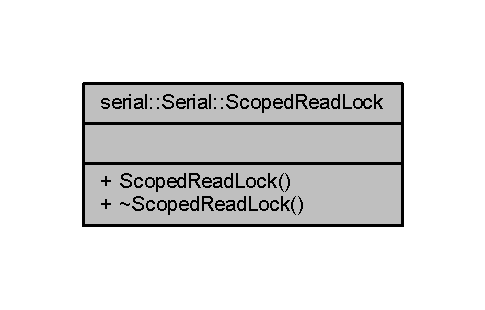
\includegraphics[width=233pt]{class_serial_1_1_scoped_read_lock__coll__graph}
\end{center}
\end{figure}
\subsection*{Public Member Functions}
\begin{DoxyCompactItemize}
\item 
\mbox{\hyperlink{class_serial_1_1_scoped_read_lock_a54f59663807d8adfe6db712ee6103503}{Scoped\+Read\+Lock}} (Serial\+Impl $\ast$pimpl)
\item 
\mbox{\hyperlink{class_serial_1_1_scoped_read_lock_a5c061909b95231cec776c40094c878b4}{$\sim$\+Scoped\+Read\+Lock}} ()
\end{DoxyCompactItemize}


\subsection{Constructor \& Destructor Documentation}
\mbox{\Hypertarget{class_serial_1_1_scoped_read_lock_a54f59663807d8adfe6db712ee6103503}\label{class_serial_1_1_scoped_read_lock_a54f59663807d8adfe6db712ee6103503}} 
\index{Serial\+::\+Scoped\+Read\+Lock@{Serial\+::\+Scoped\+Read\+Lock}!Scoped\+Read\+Lock@{Scoped\+Read\+Lock}}
\index{Scoped\+Read\+Lock@{Scoped\+Read\+Lock}!Serial\+::\+Scoped\+Read\+Lock@{Serial\+::\+Scoped\+Read\+Lock}}
\subsubsection{\texorpdfstring{Scoped\+Read\+Lock()}{ScopedReadLock()}}
{\footnotesize\ttfamily serial\+::\+Serial\+::\+Scoped\+Read\+Lock\+::\+Scoped\+Read\+Lock (\begin{DoxyParamCaption}\item[{Serial\+Impl $\ast$}]{pimpl }\end{DoxyParamCaption})\hspace{0.3cm}{\ttfamily [inline]}}

\mbox{\Hypertarget{class_serial_1_1_scoped_read_lock_a5c061909b95231cec776c40094c878b4}\label{class_serial_1_1_scoped_read_lock_a5c061909b95231cec776c40094c878b4}} 
\index{Serial\+::\+Scoped\+Read\+Lock@{Serial\+::\+Scoped\+Read\+Lock}!````~Scoped\+Read\+Lock@{$\sim$\+Scoped\+Read\+Lock}}
\index{````~Scoped\+Read\+Lock@{$\sim$\+Scoped\+Read\+Lock}!Serial\+::\+Scoped\+Read\+Lock@{Serial\+::\+Scoped\+Read\+Lock}}
\subsubsection{\texorpdfstring{$\sim$\+Scoped\+Read\+Lock()}{~ScopedReadLock()}}
{\footnotesize\ttfamily serial\+::\+Serial\+::\+Scoped\+Read\+Lock\+::$\sim$\+Scoped\+Read\+Lock (\begin{DoxyParamCaption}{ }\end{DoxyParamCaption})\hspace{0.3cm}{\ttfamily [inline]}}



The documentation for this class was generated from the following file\+:\begin{DoxyCompactItemize}
\item 
C\+:/folders/d/scripts/cpp/\+O\+P\+T3101\+S\+D\+K/\+O\+P\+T3101\+S\+D\+K/\+O\+P\+T3101\+S\+D\+K/serial\+Lib/\mbox{\hyperlink{serial_8cc}{serial.\+cc}}\end{DoxyCompactItemize}

\hypertarget{class_serial_1_1_scoped_write_lock}{}\section{serial\+:\+:Serial\+:\+:Scoped\+Write\+Lock Class Reference}
\label{class_serial_1_1_scoped_write_lock}\index{serial\+::\+Serial\+::\+Scoped\+Write\+Lock@{serial\+::\+Serial\+::\+Scoped\+Write\+Lock}}


Collaboration diagram for serial\+:\+:Serial\+:\+:Scoped\+Write\+Lock\+:\nopagebreak
\begin{figure}[H]
\begin{center}
\leavevmode
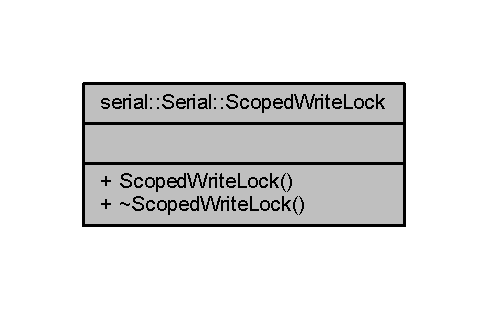
\includegraphics[width=234pt]{class_serial_1_1_scoped_write_lock__coll__graph}
\end{center}
\end{figure}
\subsection*{Public Member Functions}
\begin{DoxyCompactItemize}
\item 
\mbox{\hyperlink{class_serial_1_1_scoped_write_lock_a662173968431aee3d6f204c354b20225}{Scoped\+Write\+Lock}} (Serial\+Impl $\ast$pimpl)
\item 
\mbox{\hyperlink{class_serial_1_1_scoped_write_lock_aebeef5b2d16f409b60094cfac092ada2}{$\sim$\+Scoped\+Write\+Lock}} ()
\end{DoxyCompactItemize}


\subsection{Constructor \& Destructor Documentation}
\mbox{\Hypertarget{class_serial_1_1_scoped_write_lock_a662173968431aee3d6f204c354b20225}\label{class_serial_1_1_scoped_write_lock_a662173968431aee3d6f204c354b20225}} 
\index{Serial\+::\+Scoped\+Write\+Lock@{Serial\+::\+Scoped\+Write\+Lock}!Scoped\+Write\+Lock@{Scoped\+Write\+Lock}}
\index{Scoped\+Write\+Lock@{Scoped\+Write\+Lock}!Serial\+::\+Scoped\+Write\+Lock@{Serial\+::\+Scoped\+Write\+Lock}}
\subsubsection{\texorpdfstring{Scoped\+Write\+Lock()}{ScopedWriteLock()}}
{\footnotesize\ttfamily serial\+::\+Serial\+::\+Scoped\+Write\+Lock\+::\+Scoped\+Write\+Lock (\begin{DoxyParamCaption}\item[{Serial\+Impl $\ast$}]{pimpl }\end{DoxyParamCaption})\hspace{0.3cm}{\ttfamily [inline]}}

\mbox{\Hypertarget{class_serial_1_1_scoped_write_lock_aebeef5b2d16f409b60094cfac092ada2}\label{class_serial_1_1_scoped_write_lock_aebeef5b2d16f409b60094cfac092ada2}} 
\index{Serial\+::\+Scoped\+Write\+Lock@{Serial\+::\+Scoped\+Write\+Lock}!````~Scoped\+Write\+Lock@{$\sim$\+Scoped\+Write\+Lock}}
\index{````~Scoped\+Write\+Lock@{$\sim$\+Scoped\+Write\+Lock}!Serial\+::\+Scoped\+Write\+Lock@{Serial\+::\+Scoped\+Write\+Lock}}
\subsubsection{\texorpdfstring{$\sim$\+Scoped\+Write\+Lock()}{~ScopedWriteLock()}}
{\footnotesize\ttfamily serial\+::\+Serial\+::\+Scoped\+Write\+Lock\+::$\sim$\+Scoped\+Write\+Lock (\begin{DoxyParamCaption}{ }\end{DoxyParamCaption})\hspace{0.3cm}{\ttfamily [inline]}}



The documentation for this class was generated from the following file\+:\begin{DoxyCompactItemize}
\item 
C\+:/folders/d/scripts/cpp/\+O\+P\+T3101\+S\+D\+K/\+O\+P\+T3101\+S\+D\+K/\+O\+P\+T3101\+S\+D\+K/serial\+Lib/\mbox{\hyperlink{serial_8cc}{serial.\+cc}}\end{DoxyCompactItemize}

\hypertarget{classserial_1_1_serial}{}\section{serial\+:\+:Serial Class Reference}
\label{classserial_1_1_serial}\index{serial\+::\+Serial@{serial\+::\+Serial}}


{\ttfamily \#include $<$serial.\+h$>$}



Collaboration diagram for serial\+:\+:Serial\+:\nopagebreak
\begin{figure}[H]
\begin{center}
\leavevmode
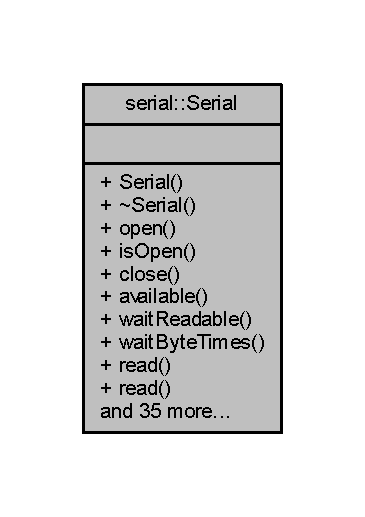
\includegraphics[width=175pt]{classserial_1_1_serial__coll__graph}
\end{center}
\end{figure}
\subsection*{Classes}
\begin{DoxyCompactItemize}
\item 
class \mbox{\hyperlink{class_serial_1_1_scoped_read_lock}{Scoped\+Read\+Lock}}
\item 
class \mbox{\hyperlink{class_serial_1_1_scoped_write_lock}{Scoped\+Write\+Lock}}
\end{DoxyCompactItemize}
\subsection*{Public Member Functions}
\begin{DoxyCompactItemize}
\item 
\mbox{\hyperlink{classserial_1_1_serial_aecbc4cc1723143805ae5a4aa79ba9332}{Serial}} (const std\+::string \&port=\char`\"{}\char`\"{}, uint32\+\_\+t baudrate=9600, \mbox{\hyperlink{structserial_1_1_timeout}{Timeout}} timeout=\mbox{\hyperlink{structserial_1_1_timeout}{Timeout}}(), \mbox{\hyperlink{namespaceserial_a00b3281fa11cea770c0b0c8a106080f8}{bytesize\+\_\+t}} bytesize=\mbox{\hyperlink{namespaceserial_a00b3281fa11cea770c0b0c8a106080f8a47f14d952cf9bed6c3f7ae5985161990}{eightbits}}, \mbox{\hyperlink{namespaceserial_a8f45d26bf7c9a06659e75b5004a50481}{parity\+\_\+t}} parity=\mbox{\hyperlink{namespaceserial_a8f45d26bf7c9a06659e75b5004a50481a31cbb2b3cf0870d1a089d66295918416}{parity\+\_\+none}}, \mbox{\hyperlink{namespaceserial_af5b116611d6628a3aa8f788fdc09f469}{stopbits\+\_\+t}} stopbits=\mbox{\hyperlink{namespaceserial_af5b116611d6628a3aa8f788fdc09f469ab70806555a14cb43e5cc43f6f3d01157}{stopbits\+\_\+one}}, \mbox{\hyperlink{namespaceserial_a93ef57a314b4e562f9eded6c15d34351}{flowcontrol\+\_\+t}} flowcontrol=\mbox{\hyperlink{namespaceserial_a93ef57a314b4e562f9eded6c15d34351a083bc02a6e8e7c6540a28654c0f95bb0}{flowcontrol\+\_\+none}})
\item 
virtual \mbox{\hyperlink{classserial_1_1_serial_a5b32c394c0ff923a4ef1c13cfb20a6ba}{$\sim$\+Serial}} ()
\item 
void \mbox{\hyperlink{classserial_1_1_serial_af3644ed1a9d899b70e9d63bb9b808d62}{open}} ()
\item 
bool \mbox{\hyperlink{classserial_1_1_serial_a5b4069da8ec84ee4331d0690b325d08d}{is\+Open}} () const
\item 
void \mbox{\hyperlink{classserial_1_1_serial_afbe59407e718bc3d22ea4a67b304db6c}{close}} ()
\item 
size\+\_\+t \mbox{\hyperlink{classserial_1_1_serial_afafe25b2f3bb0809550abdc72c51a234}{available}} ()
\item 
bool \mbox{\hyperlink{classserial_1_1_serial_ad6e395bfe91718b66f6695c10ee90e5b}{wait\+Readable}} ()
\item 
void \mbox{\hyperlink{classserial_1_1_serial_a318262c05074a9da15d410f8af29c15c}{wait\+Byte\+Times}} (size\+\_\+t count)
\item 
size\+\_\+t \mbox{\hyperlink{classserial_1_1_serial_a0261dbfb9361784ecb3eee98b85fa103}{read}} (uint8\+\_\+t $\ast$buffer, size\+\_\+t size)
\item 
size\+\_\+t \mbox{\hyperlink{classserial_1_1_serial_aa3795c6cbc96f504932dd02fd6e9538e}{read}} (std\+::vector$<$ uint8\+\_\+t $>$ \&buffer, size\+\_\+t size=1)
\item 
size\+\_\+t \mbox{\hyperlink{classserial_1_1_serial_ac47576244e34abc2e460ba99684c351f}{read}} (std\+::string \&buffer, size\+\_\+t size=1)
\item 
std\+::string \mbox{\hyperlink{classserial_1_1_serial_a6c71ad1cbacf86cead4d38b48c548405}{read}} (size\+\_\+t size=1)
\item 
size\+\_\+t \mbox{\hyperlink{classserial_1_1_serial_a24de63dfc928479a457b6caf5f74f6ad}{readline}} (std\+::string \&buffer, size\+\_\+t size=65536, std\+::string eol=\char`\"{}\textbackslash{})
\item 
std\+::string \mbox{\hyperlink{classserial_1_1_serial_a462eb4c564b888142188c2683b062524}{readline}} (size\+\_\+t size=65536, std\+::string eol=\char`\"{}\textbackslash{})
\item 
std\+::vector$<$ std\+::string $>$ \mbox{\hyperlink{classserial_1_1_serial_a2a9a1656cc1a296a5a31a682099e13c1}{readlines}} (size\+\_\+t size=65536, std\+::string eol=\char`\"{}\textbackslash{})
\item 
size\+\_\+t \mbox{\hyperlink{classserial_1_1_serial_aa020880cdff3a370ddc574f594379c3c}{write}} (const uint8\+\_\+t $\ast$data, size\+\_\+t size)
\item 
size\+\_\+t \mbox{\hyperlink{classserial_1_1_serial_a2c4180b4c7d386c84e9d0e7ef4a267d3}{write}} (const std\+::vector$<$ uint8\+\_\+t $>$ \&data)
\item 
size\+\_\+t \mbox{\hyperlink{classserial_1_1_serial_a7c92c0307b86a935f6623953eec66460}{write}} (const std\+::string \&data)
\item 
void \mbox{\hyperlink{classserial_1_1_serial_acecb0a5102ae0c944fe4b78e4adf839a}{set\+Port}} (const std\+::string \&port)
\item 
std\+::string \mbox{\hyperlink{classserial_1_1_serial_a50ceb4a9d3fe2d6e9a21ba83a3222a9b}{get\+Port}} () const
\item 
void \mbox{\hyperlink{classserial_1_1_serial_a4fc63af4b800a9f9e757414f38f3e8b3}{set\+Timeout}} (\mbox{\hyperlink{structserial_1_1_timeout}{Timeout}} \&timeout)
\item 
void \mbox{\hyperlink{classserial_1_1_serial_a4b4be39af3e1c68bc6ac09cb55788c86}{set\+Timeout}} (uint32\+\_\+t inter\+\_\+byte\+\_\+timeout, uint32\+\_\+t read\+\_\+timeout\+\_\+constant, uint32\+\_\+t read\+\_\+timeout\+\_\+multiplier, uint32\+\_\+t write\+\_\+timeout\+\_\+constant, uint32\+\_\+t write\+\_\+timeout\+\_\+multiplier)
\item 
\mbox{\hyperlink{structserial_1_1_timeout}{Timeout}} \mbox{\hyperlink{classserial_1_1_serial_a2502ea6b503c96f64b767365965c4198}{get\+Timeout}} () const
\item 
void \mbox{\hyperlink{classserial_1_1_serial_ad4f7e9edff11b464199e94a43dfd19bf}{set\+Baudrate}} (uint32\+\_\+t baudrate)
\item 
uint32\+\_\+t \mbox{\hyperlink{classserial_1_1_serial_ac7f119828de9efe1cdf559810926755f}{get\+Baudrate}} () const
\item 
void \mbox{\hyperlink{classserial_1_1_serial_adba430fd704f6898a5a1d99fd39a94fa}{set\+Bytesize}} (\mbox{\hyperlink{namespaceserial_a00b3281fa11cea770c0b0c8a106080f8}{bytesize\+\_\+t}} bytesize)
\item 
\mbox{\hyperlink{namespaceserial_a00b3281fa11cea770c0b0c8a106080f8}{bytesize\+\_\+t}} \mbox{\hyperlink{classserial_1_1_serial_ac0d2260901c4d2d99829135341a7d59c}{get\+Bytesize}} () const
\item 
void \mbox{\hyperlink{classserial_1_1_serial_a1e1896aa59ec35ac5bd263b87614ef01}{set\+Parity}} (\mbox{\hyperlink{namespaceserial_a8f45d26bf7c9a06659e75b5004a50481}{parity\+\_\+t}} parity)
\item 
\mbox{\hyperlink{namespaceserial_a8f45d26bf7c9a06659e75b5004a50481}{parity\+\_\+t}} \mbox{\hyperlink{classserial_1_1_serial_aba1b4a81903ab1b0b3ec5a49fd30b6e9}{get\+Parity}} () const
\item 
void \mbox{\hyperlink{classserial_1_1_serial_ab72284b5aab723b81013fb560bd6acc5}{set\+Stopbits}} (\mbox{\hyperlink{namespaceserial_af5b116611d6628a3aa8f788fdc09f469}{stopbits\+\_\+t}} stopbits)
\item 
\mbox{\hyperlink{namespaceserial_af5b116611d6628a3aa8f788fdc09f469}{stopbits\+\_\+t}} \mbox{\hyperlink{classserial_1_1_serial_a2bf619bd500f12fe973244f4c16e430a}{get\+Stopbits}} () const
\item 
void \mbox{\hyperlink{classserial_1_1_serial_ade41650d6bfe91b6432e5a0a60c03969}{set\+Flowcontrol}} (\mbox{\hyperlink{namespaceserial_a93ef57a314b4e562f9eded6c15d34351}{flowcontrol\+\_\+t}} flowcontrol)
\item 
\mbox{\hyperlink{namespaceserial_a93ef57a314b4e562f9eded6c15d34351}{flowcontrol\+\_\+t}} \mbox{\hyperlink{classserial_1_1_serial_a81b78424cc1dda253ee07094eac60733}{get\+Flowcontrol}} () const
\item 
void \mbox{\hyperlink{classserial_1_1_serial_a63b7abf172cad25bfc998b3b1f98310f}{flush}} ()
\item 
void \mbox{\hyperlink{classserial_1_1_serial_afa2c1f9114a37b7d140fc2292d1499b9}{flush\+Input}} ()
\item 
void \mbox{\hyperlink{classserial_1_1_serial_a256ee4bb93ab0e79d7a66b50f08dce53}{flush\+Output}} ()
\item 
void \mbox{\hyperlink{classserial_1_1_serial_ade90ff8f03525ea6d7b702fcd0f336de}{send\+Break}} (int duration)
\item 
void \mbox{\hyperlink{classserial_1_1_serial_a2a27912b1ca5cdad4a4aba7b9ddbc206}{set\+Break}} (bool level=true)
\item 
void \mbox{\hyperlink{classserial_1_1_serial_ab43ddc05e5d69ff2778f698aa7062370}{set\+R\+TS}} (bool level=true)
\item 
void \mbox{\hyperlink{classserial_1_1_serial_ac9b0bbf613a5fe68f05d1d40181a1bb3}{set\+D\+TR}} (bool level=true)
\item 
bool \mbox{\hyperlink{classserial_1_1_serial_a419dc984258956a5adb41fb8c86f5449}{wait\+For\+Change}} ()
\item 
bool \mbox{\hyperlink{classserial_1_1_serial_a809f048546c4c72b74e205139b97648c}{get\+C\+TS}} ()
\item 
bool \mbox{\hyperlink{classserial_1_1_serial_a6b9a0c485e1fe599dbb5e9e15b1a65d6}{get\+D\+SR}} ()
\item 
bool \mbox{\hyperlink{classserial_1_1_serial_afb96e6968f040c4bff7576095f4ba6e7}{get\+RI}} ()
\item 
bool \mbox{\hyperlink{classserial_1_1_serial_a9795a3e83e6745a14c64f657e68061fb}{get\+CD}} ()
\end{DoxyCompactItemize}


\subsection{Detailed Description}
Class that provides a portable serial port interface. 

\subsection{Constructor \& Destructor Documentation}
\mbox{\Hypertarget{classserial_1_1_serial_aecbc4cc1723143805ae5a4aa79ba9332}\label{classserial_1_1_serial_aecbc4cc1723143805ae5a4aa79ba9332}} 
\index{serial\+::\+Serial@{serial\+::\+Serial}!Serial@{Serial}}
\index{Serial@{Serial}!serial\+::\+Serial@{serial\+::\+Serial}}
\subsubsection{\texorpdfstring{Serial()}{Serial()}}
{\footnotesize\ttfamily serial\+::\+Serial\+::\+Serial (\begin{DoxyParamCaption}\item[{const std\+::string \&}]{port = {\ttfamily \char`\"{}\char`\"{}},  }\item[{uint32\+\_\+t}]{baudrate = {\ttfamily 9600},  }\item[{\mbox{\hyperlink{structserial_1_1_timeout}{Timeout}}}]{timeout = {\ttfamily \mbox{\hyperlink{structserial_1_1_timeout}{Timeout}}()},  }\item[{\mbox{\hyperlink{namespaceserial_a00b3281fa11cea770c0b0c8a106080f8}{bytesize\+\_\+t}}}]{bytesize = {\ttfamily \mbox{\hyperlink{namespaceserial_a00b3281fa11cea770c0b0c8a106080f8a47f14d952cf9bed6c3f7ae5985161990}{eightbits}}},  }\item[{\mbox{\hyperlink{namespaceserial_a8f45d26bf7c9a06659e75b5004a50481}{parity\+\_\+t}}}]{parity = {\ttfamily \mbox{\hyperlink{namespaceserial_a8f45d26bf7c9a06659e75b5004a50481a31cbb2b3cf0870d1a089d66295918416}{parity\+\_\+none}}},  }\item[{\mbox{\hyperlink{namespaceserial_af5b116611d6628a3aa8f788fdc09f469}{stopbits\+\_\+t}}}]{stopbits = {\ttfamily \mbox{\hyperlink{namespaceserial_af5b116611d6628a3aa8f788fdc09f469ab70806555a14cb43e5cc43f6f3d01157}{stopbits\+\_\+one}}},  }\item[{\mbox{\hyperlink{namespaceserial_a93ef57a314b4e562f9eded6c15d34351}{flowcontrol\+\_\+t}}}]{flowcontrol = {\ttfamily \mbox{\hyperlink{namespaceserial_a93ef57a314b4e562f9eded6c15d34351a083bc02a6e8e7c6540a28654c0f95bb0}{flowcontrol\+\_\+none}}} }\end{DoxyParamCaption})}

Creates a \mbox{\hyperlink{classserial_1_1_serial}{Serial}} object and opens the port if a port is specified, otherwise it remains closed until \mbox{\hyperlink{classserial_1_1_serial_af3644ed1a9d899b70e9d63bb9b808d62}{serial\+::\+Serial\+::open}} is called.


\begin{DoxyParams}{Parameters}
{\em port} & A std\+::string containing the address of the serial port, which would be something like \textquotesingle{}C\+O\+M1\textquotesingle{} on Windows and \textquotesingle{}/dev/tty\+S0\textquotesingle{} on Linux.\\
\hline
{\em baudrate} & An unsigned 32-\/bit integer that represents the baudrate\\
\hline
{\em timeout} & A \mbox{\hyperlink{structserial_1_1_timeout}{serial\+::\+Timeout}} struct that defines the timeout conditions for the serial port. \\
\hline
\end{DoxyParams}
\begin{DoxySeeAlso}{See also}
\mbox{\hyperlink{structserial_1_1_timeout}{serial\+::\+Timeout}}
\end{DoxySeeAlso}

\begin{DoxyParams}{Parameters}
{\em bytesize} & Size of each byte in the serial transmission of data, default is eightbits, possible values are\+: fivebits, sixbits, sevenbits, eightbits\\
\hline
{\em parity} & Method of parity, default is parity\+\_\+none, possible values are\+: parity\+\_\+none, parity\+\_\+odd, parity\+\_\+even\\
\hline
{\em stopbits} & Number of stop bits used, default is stopbits\+\_\+one, possible values are\+: stopbits\+\_\+one, stopbits\+\_\+one\+\_\+point\+\_\+five, stopbits\+\_\+two\\
\hline
{\em flowcontrol} & Type of flowcontrol used, default is flowcontrol\+\_\+none, possible values are\+: flowcontrol\+\_\+none, flowcontrol\+\_\+software, flowcontrol\+\_\+hardware\\
\hline
\end{DoxyParams}

\begin{DoxyExceptions}{Exceptions}
{\em \mbox{\hyperlink{classserial_1_1_port_not_opened_exception}{serial\+::\+Port\+Not\+Opened\+Exception}}} & \\
\hline
{\em \mbox{\hyperlink{classserial_1_1_i_o_exception}{serial\+::\+I\+O\+Exception}}} & \\
\hline
{\em std\+::invalid\+\_\+argument} & \\
\hline
\end{DoxyExceptions}
\mbox{\Hypertarget{classserial_1_1_serial_a5b32c394c0ff923a4ef1c13cfb20a6ba}\label{classserial_1_1_serial_a5b32c394c0ff923a4ef1c13cfb20a6ba}} 
\index{serial\+::\+Serial@{serial\+::\+Serial}!````~Serial@{$\sim$\+Serial}}
\index{````~Serial@{$\sim$\+Serial}!serial\+::\+Serial@{serial\+::\+Serial}}
\subsubsection{\texorpdfstring{$\sim$\+Serial()}{~Serial()}}
{\footnotesize\ttfamily Serial\+::$\sim$\+Serial (\begin{DoxyParamCaption}{ }\end{DoxyParamCaption})\hspace{0.3cm}{\ttfamily [virtual]}}

Destructor 

\subsection{Member Function Documentation}
\mbox{\Hypertarget{classserial_1_1_serial_afafe25b2f3bb0809550abdc72c51a234}\label{classserial_1_1_serial_afafe25b2f3bb0809550abdc72c51a234}} 
\index{serial\+::\+Serial@{serial\+::\+Serial}!available@{available}}
\index{available@{available}!serial\+::\+Serial@{serial\+::\+Serial}}
\subsubsection{\texorpdfstring{available()}{available()}}
{\footnotesize\ttfamily size\+\_\+t Serial\+::available (\begin{DoxyParamCaption}{ }\end{DoxyParamCaption})}

Return the number of characters in the buffer. \mbox{\Hypertarget{classserial_1_1_serial_afbe59407e718bc3d22ea4a67b304db6c}\label{classserial_1_1_serial_afbe59407e718bc3d22ea4a67b304db6c}} 
\index{serial\+::\+Serial@{serial\+::\+Serial}!close@{close}}
\index{close@{close}!serial\+::\+Serial@{serial\+::\+Serial}}
\subsubsection{\texorpdfstring{close()}{close()}}
{\footnotesize\ttfamily void Serial\+::close (\begin{DoxyParamCaption}{ }\end{DoxyParamCaption})}

Closes the serial port. \mbox{\Hypertarget{classserial_1_1_serial_a63b7abf172cad25bfc998b3b1f98310f}\label{classserial_1_1_serial_a63b7abf172cad25bfc998b3b1f98310f}} 
\index{serial\+::\+Serial@{serial\+::\+Serial}!flush@{flush}}
\index{flush@{flush}!serial\+::\+Serial@{serial\+::\+Serial}}
\subsubsection{\texorpdfstring{flush()}{flush()}}
{\footnotesize\ttfamily void Serial\+::flush (\begin{DoxyParamCaption}{ }\end{DoxyParamCaption})}

Flush the input and output buffers \mbox{\Hypertarget{classserial_1_1_serial_afa2c1f9114a37b7d140fc2292d1499b9}\label{classserial_1_1_serial_afa2c1f9114a37b7d140fc2292d1499b9}} 
\index{serial\+::\+Serial@{serial\+::\+Serial}!flush\+Input@{flush\+Input}}
\index{flush\+Input@{flush\+Input}!serial\+::\+Serial@{serial\+::\+Serial}}
\subsubsection{\texorpdfstring{flush\+Input()}{flushInput()}}
{\footnotesize\ttfamily void Serial\+::flush\+Input (\begin{DoxyParamCaption}{ }\end{DoxyParamCaption})}

Flush only the input buffer \mbox{\Hypertarget{classserial_1_1_serial_a256ee4bb93ab0e79d7a66b50f08dce53}\label{classserial_1_1_serial_a256ee4bb93ab0e79d7a66b50f08dce53}} 
\index{serial\+::\+Serial@{serial\+::\+Serial}!flush\+Output@{flush\+Output}}
\index{flush\+Output@{flush\+Output}!serial\+::\+Serial@{serial\+::\+Serial}}
\subsubsection{\texorpdfstring{flush\+Output()}{flushOutput()}}
{\footnotesize\ttfamily void Serial\+::flush\+Output (\begin{DoxyParamCaption}{ }\end{DoxyParamCaption})}

Flush only the output buffer \mbox{\Hypertarget{classserial_1_1_serial_ac7f119828de9efe1cdf559810926755f}\label{classserial_1_1_serial_ac7f119828de9efe1cdf559810926755f}} 
\index{serial\+::\+Serial@{serial\+::\+Serial}!get\+Baudrate@{get\+Baudrate}}
\index{get\+Baudrate@{get\+Baudrate}!serial\+::\+Serial@{serial\+::\+Serial}}
\subsubsection{\texorpdfstring{get\+Baudrate()}{getBaudrate()}}
{\footnotesize\ttfamily uint32\+\_\+t Serial\+::get\+Baudrate (\begin{DoxyParamCaption}{ }\end{DoxyParamCaption}) const}

Gets the baudrate for the serial port.

\begin{DoxyReturn}{Returns}
An integer that sets the baud rate for the serial port.
\end{DoxyReturn}
\begin{DoxySeeAlso}{See also}
\mbox{\hyperlink{classserial_1_1_serial_ad4f7e9edff11b464199e94a43dfd19bf}{Serial\+::set\+Baudrate}}
\end{DoxySeeAlso}

\begin{DoxyExceptions}{Exceptions}
{\em std\+::invalid\+\_\+argument} & \\
\hline
\end{DoxyExceptions}
\mbox{\Hypertarget{classserial_1_1_serial_ac0d2260901c4d2d99829135341a7d59c}\label{classserial_1_1_serial_ac0d2260901c4d2d99829135341a7d59c}} 
\index{serial\+::\+Serial@{serial\+::\+Serial}!get\+Bytesize@{get\+Bytesize}}
\index{get\+Bytesize@{get\+Bytesize}!serial\+::\+Serial@{serial\+::\+Serial}}
\subsubsection{\texorpdfstring{get\+Bytesize()}{getBytesize()}}
{\footnotesize\ttfamily \mbox{\hyperlink{namespaceserial_a00b3281fa11cea770c0b0c8a106080f8}{bytesize\+\_\+t}} Serial\+::get\+Bytesize (\begin{DoxyParamCaption}{ }\end{DoxyParamCaption}) const}

Gets the bytesize for the serial port.

\begin{DoxySeeAlso}{See also}
\mbox{\hyperlink{classserial_1_1_serial_adba430fd704f6898a5a1d99fd39a94fa}{Serial\+::set\+Bytesize}}
\end{DoxySeeAlso}

\begin{DoxyExceptions}{Exceptions}
{\em std\+::invalid\+\_\+argument} & \\
\hline
\end{DoxyExceptions}
\mbox{\Hypertarget{classserial_1_1_serial_a9795a3e83e6745a14c64f657e68061fb}\label{classserial_1_1_serial_a9795a3e83e6745a14c64f657e68061fb}} 
\index{serial\+::\+Serial@{serial\+::\+Serial}!get\+CD@{get\+CD}}
\index{get\+CD@{get\+CD}!serial\+::\+Serial@{serial\+::\+Serial}}
\subsubsection{\texorpdfstring{get\+C\+D()}{getCD()}}
{\footnotesize\ttfamily bool Serial\+::get\+CD (\begin{DoxyParamCaption}{ }\end{DoxyParamCaption})}

Returns the current status of the CD line. \mbox{\Hypertarget{classserial_1_1_serial_a809f048546c4c72b74e205139b97648c}\label{classserial_1_1_serial_a809f048546c4c72b74e205139b97648c}} 
\index{serial\+::\+Serial@{serial\+::\+Serial}!get\+C\+TS@{get\+C\+TS}}
\index{get\+C\+TS@{get\+C\+TS}!serial\+::\+Serial@{serial\+::\+Serial}}
\subsubsection{\texorpdfstring{get\+C\+T\+S()}{getCTS()}}
{\footnotesize\ttfamily bool Serial\+::get\+C\+TS (\begin{DoxyParamCaption}{ }\end{DoxyParamCaption})}

Returns the current status of the C\+TS line. \mbox{\Hypertarget{classserial_1_1_serial_a6b9a0c485e1fe599dbb5e9e15b1a65d6}\label{classserial_1_1_serial_a6b9a0c485e1fe599dbb5e9e15b1a65d6}} 
\index{serial\+::\+Serial@{serial\+::\+Serial}!get\+D\+SR@{get\+D\+SR}}
\index{get\+D\+SR@{get\+D\+SR}!serial\+::\+Serial@{serial\+::\+Serial}}
\subsubsection{\texorpdfstring{get\+D\+S\+R()}{getDSR()}}
{\footnotesize\ttfamily bool Serial\+::get\+D\+SR (\begin{DoxyParamCaption}{ }\end{DoxyParamCaption})}

Returns the current status of the D\+SR line. \mbox{\Hypertarget{classserial_1_1_serial_a81b78424cc1dda253ee07094eac60733}\label{classserial_1_1_serial_a81b78424cc1dda253ee07094eac60733}} 
\index{serial\+::\+Serial@{serial\+::\+Serial}!get\+Flowcontrol@{get\+Flowcontrol}}
\index{get\+Flowcontrol@{get\+Flowcontrol}!serial\+::\+Serial@{serial\+::\+Serial}}
\subsubsection{\texorpdfstring{get\+Flowcontrol()}{getFlowcontrol()}}
{\footnotesize\ttfamily \mbox{\hyperlink{namespaceserial_a93ef57a314b4e562f9eded6c15d34351}{flowcontrol\+\_\+t}} Serial\+::get\+Flowcontrol (\begin{DoxyParamCaption}{ }\end{DoxyParamCaption}) const}

Gets the flow control for the serial port.

\begin{DoxySeeAlso}{See also}
\mbox{\hyperlink{classserial_1_1_serial_ade41650d6bfe91b6432e5a0a60c03969}{Serial\+::set\+Flowcontrol}}
\end{DoxySeeAlso}

\begin{DoxyExceptions}{Exceptions}
{\em std\+::invalid\+\_\+argument} & \\
\hline
\end{DoxyExceptions}
\mbox{\Hypertarget{classserial_1_1_serial_aba1b4a81903ab1b0b3ec5a49fd30b6e9}\label{classserial_1_1_serial_aba1b4a81903ab1b0b3ec5a49fd30b6e9}} 
\index{serial\+::\+Serial@{serial\+::\+Serial}!get\+Parity@{get\+Parity}}
\index{get\+Parity@{get\+Parity}!serial\+::\+Serial@{serial\+::\+Serial}}
\subsubsection{\texorpdfstring{get\+Parity()}{getParity()}}
{\footnotesize\ttfamily \mbox{\hyperlink{namespaceserial_a8f45d26bf7c9a06659e75b5004a50481}{parity\+\_\+t}} Serial\+::get\+Parity (\begin{DoxyParamCaption}{ }\end{DoxyParamCaption}) const}

Gets the parity for the serial port.

\begin{DoxySeeAlso}{See also}
\mbox{\hyperlink{classserial_1_1_serial_a1e1896aa59ec35ac5bd263b87614ef01}{Serial\+::set\+Parity}}
\end{DoxySeeAlso}

\begin{DoxyExceptions}{Exceptions}
{\em std\+::invalid\+\_\+argument} & \\
\hline
\end{DoxyExceptions}
\mbox{\Hypertarget{classserial_1_1_serial_a50ceb4a9d3fe2d6e9a21ba83a3222a9b}\label{classserial_1_1_serial_a50ceb4a9d3fe2d6e9a21ba83a3222a9b}} 
\index{serial\+::\+Serial@{serial\+::\+Serial}!get\+Port@{get\+Port}}
\index{get\+Port@{get\+Port}!serial\+::\+Serial@{serial\+::\+Serial}}
\subsubsection{\texorpdfstring{get\+Port()}{getPort()}}
{\footnotesize\ttfamily string Serial\+::get\+Port (\begin{DoxyParamCaption}{ }\end{DoxyParamCaption}) const}

Gets the serial port identifier.

\begin{DoxySeeAlso}{See also}
\mbox{\hyperlink{classserial_1_1_serial_acecb0a5102ae0c944fe4b78e4adf839a}{Serial\+::set\+Port}}
\end{DoxySeeAlso}

\begin{DoxyExceptions}{Exceptions}
{\em std\+::invalid\+\_\+argument} & \\
\hline
\end{DoxyExceptions}
\mbox{\Hypertarget{classserial_1_1_serial_afb96e6968f040c4bff7576095f4ba6e7}\label{classserial_1_1_serial_afb96e6968f040c4bff7576095f4ba6e7}} 
\index{serial\+::\+Serial@{serial\+::\+Serial}!get\+RI@{get\+RI}}
\index{get\+RI@{get\+RI}!serial\+::\+Serial@{serial\+::\+Serial}}
\subsubsection{\texorpdfstring{get\+R\+I()}{getRI()}}
{\footnotesize\ttfamily bool Serial\+::get\+RI (\begin{DoxyParamCaption}{ }\end{DoxyParamCaption})}

Returns the current status of the RI line. \mbox{\Hypertarget{classserial_1_1_serial_a2bf619bd500f12fe973244f4c16e430a}\label{classserial_1_1_serial_a2bf619bd500f12fe973244f4c16e430a}} 
\index{serial\+::\+Serial@{serial\+::\+Serial}!get\+Stopbits@{get\+Stopbits}}
\index{get\+Stopbits@{get\+Stopbits}!serial\+::\+Serial@{serial\+::\+Serial}}
\subsubsection{\texorpdfstring{get\+Stopbits()}{getStopbits()}}
{\footnotesize\ttfamily \mbox{\hyperlink{namespaceserial_af5b116611d6628a3aa8f788fdc09f469}{stopbits\+\_\+t}} Serial\+::get\+Stopbits (\begin{DoxyParamCaption}{ }\end{DoxyParamCaption}) const}

Gets the stopbits for the serial port.

\begin{DoxySeeAlso}{See also}
\mbox{\hyperlink{classserial_1_1_serial_ab72284b5aab723b81013fb560bd6acc5}{Serial\+::set\+Stopbits}}
\end{DoxySeeAlso}

\begin{DoxyExceptions}{Exceptions}
{\em std\+::invalid\+\_\+argument} & \\
\hline
\end{DoxyExceptions}
\mbox{\Hypertarget{classserial_1_1_serial_a2502ea6b503c96f64b767365965c4198}\label{classserial_1_1_serial_a2502ea6b503c96f64b767365965c4198}} 
\index{serial\+::\+Serial@{serial\+::\+Serial}!get\+Timeout@{get\+Timeout}}
\index{get\+Timeout@{get\+Timeout}!serial\+::\+Serial@{serial\+::\+Serial}}
\subsubsection{\texorpdfstring{get\+Timeout()}{getTimeout()}}
{\footnotesize\ttfamily \mbox{\hyperlink{structserial_1_1_timeout}{serial\+::\+Timeout}} Serial\+::get\+Timeout (\begin{DoxyParamCaption}{ }\end{DoxyParamCaption}) const}

Gets the timeout for reads in seconds.

\begin{DoxyReturn}{Returns}
A \mbox{\hyperlink{structserial_1_1_timeout}{Timeout}} struct containing the inter\+\_\+byte\+\_\+timeout, and read and write timeout constants and multipliers.
\end{DoxyReturn}
\begin{DoxySeeAlso}{See also}
\mbox{\hyperlink{classserial_1_1_serial_a4fc63af4b800a9f9e757414f38f3e8b3}{Serial\+::set\+Timeout}} 
\end{DoxySeeAlso}
\mbox{\Hypertarget{classserial_1_1_serial_a5b4069da8ec84ee4331d0690b325d08d}\label{classserial_1_1_serial_a5b4069da8ec84ee4331d0690b325d08d}} 
\index{serial\+::\+Serial@{serial\+::\+Serial}!is\+Open@{is\+Open}}
\index{is\+Open@{is\+Open}!serial\+::\+Serial@{serial\+::\+Serial}}
\subsubsection{\texorpdfstring{is\+Open()}{isOpen()}}
{\footnotesize\ttfamily bool Serial\+::is\+Open (\begin{DoxyParamCaption}{ }\end{DoxyParamCaption}) const}

Gets the open status of the serial port.

\begin{DoxyReturn}{Returns}
Returns true if the port is open, false otherwise. 
\end{DoxyReturn}
\mbox{\Hypertarget{classserial_1_1_serial_af3644ed1a9d899b70e9d63bb9b808d62}\label{classserial_1_1_serial_af3644ed1a9d899b70e9d63bb9b808d62}} 
\index{serial\+::\+Serial@{serial\+::\+Serial}!open@{open}}
\index{open@{open}!serial\+::\+Serial@{serial\+::\+Serial}}
\subsubsection{\texorpdfstring{open()}{open()}}
{\footnotesize\ttfamily void Serial\+::open (\begin{DoxyParamCaption}{ }\end{DoxyParamCaption})}

Opens the serial port as long as the port is set and the port isn\textquotesingle{}t already open.

If the port is provided to the constructor then an explicit call to open is not needed.

\begin{DoxySeeAlso}{See also}
\mbox{\hyperlink{classserial_1_1_serial_aecbc4cc1723143805ae5a4aa79ba9332}{Serial\+::\+Serial}}
\end{DoxySeeAlso}

\begin{DoxyExceptions}{Exceptions}
{\em std\+::invalid\+\_\+argument} & \\
\hline
{\em \mbox{\hyperlink{classserial_1_1_serial_exception}{serial\+::\+Serial\+Exception}}} & \\
\hline
{\em \mbox{\hyperlink{classserial_1_1_i_o_exception}{serial\+::\+I\+O\+Exception}}} & \\
\hline
\end{DoxyExceptions}
\mbox{\Hypertarget{classserial_1_1_serial_a0261dbfb9361784ecb3eee98b85fa103}\label{classserial_1_1_serial_a0261dbfb9361784ecb3eee98b85fa103}} 
\index{serial\+::\+Serial@{serial\+::\+Serial}!read@{read}}
\index{read@{read}!serial\+::\+Serial@{serial\+::\+Serial}}
\subsubsection{\texorpdfstring{read()}{read()}\hspace{0.1cm}{\footnotesize\ttfamily [1/4]}}
{\footnotesize\ttfamily size\+\_\+t Serial\+::read (\begin{DoxyParamCaption}\item[{uint8\+\_\+t $\ast$}]{buffer,  }\item[{size\+\_\+t}]{size }\end{DoxyParamCaption})}

Read a given amount of bytes from the serial port into a given buffer.

The read function will return in one of three cases\+:
\begin{DoxyItemize}
\item The number of requested bytes was read.
\begin{DoxyItemize}
\item In this case the number of bytes requested will match the size\+\_\+t returned by read.
\end{DoxyItemize}
\item A timeout occurred, in this case the number of bytes read will not match the amount requested, but no exception will be thrown. One of two possible timeouts occurred\+:
\begin{DoxyItemize}
\item The inter byte timeout expired, this means that number of milliseconds elapsed between receiving bytes from the serial port exceeded the inter byte timeout.
\item The total timeout expired, which is calculated by multiplying the read timeout multiplier by the number of requested bytes and then added to the read timeout constant. If that total number of milliseconds elapses after the initial call to read a timeout will occur.
\end{DoxyItemize}
\item An exception occurred, in this case an actual exception will be thrown.
\end{DoxyItemize}


\begin{DoxyParams}{Parameters}
{\em buffer} & An uint8\+\_\+t array of at least the requested size. \\
\hline
{\em size} & A size\+\_\+t defining how many bytes to be read.\\
\hline
\end{DoxyParams}
\begin{DoxyReturn}{Returns}
A size\+\_\+t representing the number of bytes read as a result of the call to read.
\end{DoxyReturn}

\begin{DoxyExceptions}{Exceptions}
{\em \mbox{\hyperlink{classserial_1_1_port_not_opened_exception}{serial\+::\+Port\+Not\+Opened\+Exception}}} & \\
\hline
{\em \mbox{\hyperlink{classserial_1_1_serial_exception}{serial\+::\+Serial\+Exception}}} & \\
\hline
\end{DoxyExceptions}
\mbox{\Hypertarget{classserial_1_1_serial_aa3795c6cbc96f504932dd02fd6e9538e}\label{classserial_1_1_serial_aa3795c6cbc96f504932dd02fd6e9538e}} 
\index{serial\+::\+Serial@{serial\+::\+Serial}!read@{read}}
\index{read@{read}!serial\+::\+Serial@{serial\+::\+Serial}}
\subsubsection{\texorpdfstring{read()}{read()}\hspace{0.1cm}{\footnotesize\ttfamily [2/4]}}
{\footnotesize\ttfamily size\+\_\+t Serial\+::read (\begin{DoxyParamCaption}\item[{std\+::vector$<$ uint8\+\_\+t $>$ \&}]{buffer,  }\item[{size\+\_\+t}]{size = {\ttfamily 1} }\end{DoxyParamCaption})}

Read a given amount of bytes from the serial port into a give buffer.


\begin{DoxyParams}{Parameters}
{\em buffer} & A reference to a std\+::vector of uint8\+\_\+t. \\
\hline
{\em size} & A size\+\_\+t defining how many bytes to be read.\\
\hline
\end{DoxyParams}
\begin{DoxyReturn}{Returns}
A size\+\_\+t representing the number of bytes read as a result of the call to read.
\end{DoxyReturn}

\begin{DoxyExceptions}{Exceptions}
{\em \mbox{\hyperlink{classserial_1_1_port_not_opened_exception}{serial\+::\+Port\+Not\+Opened\+Exception}}} & \\
\hline
{\em \mbox{\hyperlink{classserial_1_1_serial_exception}{serial\+::\+Serial\+Exception}}} & \\
\hline
\end{DoxyExceptions}
\mbox{\Hypertarget{classserial_1_1_serial_ac47576244e34abc2e460ba99684c351f}\label{classserial_1_1_serial_ac47576244e34abc2e460ba99684c351f}} 
\index{serial\+::\+Serial@{serial\+::\+Serial}!read@{read}}
\index{read@{read}!serial\+::\+Serial@{serial\+::\+Serial}}
\subsubsection{\texorpdfstring{read()}{read()}\hspace{0.1cm}{\footnotesize\ttfamily [3/4]}}
{\footnotesize\ttfamily size\+\_\+t Serial\+::read (\begin{DoxyParamCaption}\item[{std\+::string \&}]{buffer,  }\item[{size\+\_\+t}]{size = {\ttfamily 1} }\end{DoxyParamCaption})}

Read a given amount of bytes from the serial port into a give buffer.


\begin{DoxyParams}{Parameters}
{\em buffer} & A reference to a std\+::string. \\
\hline
{\em size} & A size\+\_\+t defining how many bytes to be read.\\
\hline
\end{DoxyParams}
\begin{DoxyReturn}{Returns}
A size\+\_\+t representing the number of bytes read as a result of the call to read.
\end{DoxyReturn}

\begin{DoxyExceptions}{Exceptions}
{\em \mbox{\hyperlink{classserial_1_1_port_not_opened_exception}{serial\+::\+Port\+Not\+Opened\+Exception}}} & \\
\hline
{\em \mbox{\hyperlink{classserial_1_1_serial_exception}{serial\+::\+Serial\+Exception}}} & \\
\hline
\end{DoxyExceptions}
\mbox{\Hypertarget{classserial_1_1_serial_a6c71ad1cbacf86cead4d38b48c548405}\label{classserial_1_1_serial_a6c71ad1cbacf86cead4d38b48c548405}} 
\index{serial\+::\+Serial@{serial\+::\+Serial}!read@{read}}
\index{read@{read}!serial\+::\+Serial@{serial\+::\+Serial}}
\subsubsection{\texorpdfstring{read()}{read()}\hspace{0.1cm}{\footnotesize\ttfamily [4/4]}}
{\footnotesize\ttfamily string Serial\+::read (\begin{DoxyParamCaption}\item[{size\+\_\+t}]{size = {\ttfamily 1} }\end{DoxyParamCaption})}

Read a given amount of bytes from the serial port and return a string containing the data.


\begin{DoxyParams}{Parameters}
{\em size} & A size\+\_\+t defining how many bytes to be read.\\
\hline
\end{DoxyParams}
\begin{DoxyReturn}{Returns}
A std\+::string containing the data read from the port.
\end{DoxyReturn}

\begin{DoxyExceptions}{Exceptions}
{\em \mbox{\hyperlink{classserial_1_1_port_not_opened_exception}{serial\+::\+Port\+Not\+Opened\+Exception}}} & \\
\hline
{\em \mbox{\hyperlink{classserial_1_1_serial_exception}{serial\+::\+Serial\+Exception}}} & \\
\hline
\end{DoxyExceptions}
\mbox{\Hypertarget{classserial_1_1_serial_a24de63dfc928479a457b6caf5f74f6ad}\label{classserial_1_1_serial_a24de63dfc928479a457b6caf5f74f6ad}} 
\index{serial\+::\+Serial@{serial\+::\+Serial}!readline@{readline}}
\index{readline@{readline}!serial\+::\+Serial@{serial\+::\+Serial}}
\subsubsection{\texorpdfstring{readline()}{readline()}\hspace{0.1cm}{\footnotesize\ttfamily [1/2]}}
{\footnotesize\ttfamily size\+\_\+t serial\+::\+Serial\+::readline (\begin{DoxyParamCaption}\item[{std\+::string \&}]{buffer,  }\item[{size\+\_\+t}]{size = {\ttfamily 65536} }\end{DoxyParamCaption})}

Reads in a line or until a given delimiter has been processed.

Reads from the serial port until a single line has been read.


\begin{DoxyParams}{Parameters}
{\em buffer} & A std\+::string reference used to store the data. \\
\hline
{\em size} & A maximum length of a line, defaults to 65536 (2$^\wedge$16) \\
\hline
{\em eol} & A string to match against for the E\+OL.\\
\hline
\end{DoxyParams}
\begin{DoxyReturn}{Returns}
A size\+\_\+t representing the number of bytes read.
\end{DoxyReturn}

\begin{DoxyExceptions}{Exceptions}
{\em \mbox{\hyperlink{classserial_1_1_port_not_opened_exception}{serial\+::\+Port\+Not\+Opened\+Exception}}} & \\
\hline
{\em \mbox{\hyperlink{classserial_1_1_serial_exception}{serial\+::\+Serial\+Exception}}} & \\
\hline
\end{DoxyExceptions}
\mbox{\Hypertarget{classserial_1_1_serial_a462eb4c564b888142188c2683b062524}\label{classserial_1_1_serial_a462eb4c564b888142188c2683b062524}} 
\index{serial\+::\+Serial@{serial\+::\+Serial}!readline@{readline}}
\index{readline@{readline}!serial\+::\+Serial@{serial\+::\+Serial}}
\subsubsection{\texorpdfstring{readline()}{readline()}\hspace{0.1cm}{\footnotesize\ttfamily [2/2]}}
{\footnotesize\ttfamily std\+::string serial\+::\+Serial\+::readline (\begin{DoxyParamCaption}\item[{size\+\_\+t}]{size = {\ttfamily 65536} }\end{DoxyParamCaption})}

Reads in a line or until a given delimiter has been processed.

Reads from the serial port until a single line has been read.


\begin{DoxyParams}{Parameters}
{\em size} & A maximum length of a line, defaults to 65536 (2$^\wedge$16) \\
\hline
{\em eol} & A string to match against for the E\+OL.\\
\hline
\end{DoxyParams}
\begin{DoxyReturn}{Returns}
A std\+::string containing the line.
\end{DoxyReturn}

\begin{DoxyExceptions}{Exceptions}
{\em \mbox{\hyperlink{classserial_1_1_port_not_opened_exception}{serial\+::\+Port\+Not\+Opened\+Exception}}} & \\
\hline
{\em \mbox{\hyperlink{classserial_1_1_serial_exception}{serial\+::\+Serial\+Exception}}} & \\
\hline
\end{DoxyExceptions}
\mbox{\Hypertarget{classserial_1_1_serial_a2a9a1656cc1a296a5a31a682099e13c1}\label{classserial_1_1_serial_a2a9a1656cc1a296a5a31a682099e13c1}} 
\index{serial\+::\+Serial@{serial\+::\+Serial}!readlines@{readlines}}
\index{readlines@{readlines}!serial\+::\+Serial@{serial\+::\+Serial}}
\subsubsection{\texorpdfstring{readlines()}{readlines()}}
{\footnotesize\ttfamily vector$<$ string $>$ Serial\+::readlines (\begin{DoxyParamCaption}\item[{size\+\_\+t}]{size = {\ttfamily 65536},  }\item[{std\+::string}]{eol = {\ttfamily \char`\"{}\textbackslash{}n\char`\"{}} }\end{DoxyParamCaption})}

Reads in multiple lines until the serial port times out.

This requires a timeout $>$ 0 before it can be run. It will read until a timeout occurs and return a list of strings.


\begin{DoxyParams}{Parameters}
{\em size} & A maximum length of combined lines, defaults to 65536 (2$^\wedge$16)\\
\hline
{\em eol} & A string to match against for the E\+OL.\\
\hline
\end{DoxyParams}
\begin{DoxyReturn}{Returns}
A vector$<$string$>$ containing the lines.
\end{DoxyReturn}

\begin{DoxyExceptions}{Exceptions}
{\em \mbox{\hyperlink{classserial_1_1_port_not_opened_exception}{serial\+::\+Port\+Not\+Opened\+Exception}}} & \\
\hline
{\em \mbox{\hyperlink{classserial_1_1_serial_exception}{serial\+::\+Serial\+Exception}}} & \\
\hline
\end{DoxyExceptions}
\mbox{\Hypertarget{classserial_1_1_serial_ade90ff8f03525ea6d7b702fcd0f336de}\label{classserial_1_1_serial_ade90ff8f03525ea6d7b702fcd0f336de}} 
\index{serial\+::\+Serial@{serial\+::\+Serial}!send\+Break@{send\+Break}}
\index{send\+Break@{send\+Break}!serial\+::\+Serial@{serial\+::\+Serial}}
\subsubsection{\texorpdfstring{send\+Break()}{sendBreak()}}
{\footnotesize\ttfamily void Serial\+::send\+Break (\begin{DoxyParamCaption}\item[{int}]{duration }\end{DoxyParamCaption})}

Sends the R\+S-\/232 break signal. See tcsendbreak(3). \mbox{\Hypertarget{classserial_1_1_serial_ad4f7e9edff11b464199e94a43dfd19bf}\label{classserial_1_1_serial_ad4f7e9edff11b464199e94a43dfd19bf}} 
\index{serial\+::\+Serial@{serial\+::\+Serial}!set\+Baudrate@{set\+Baudrate}}
\index{set\+Baudrate@{set\+Baudrate}!serial\+::\+Serial@{serial\+::\+Serial}}
\subsubsection{\texorpdfstring{set\+Baudrate()}{setBaudrate()}}
{\footnotesize\ttfamily void Serial\+::set\+Baudrate (\begin{DoxyParamCaption}\item[{uint32\+\_\+t}]{baudrate }\end{DoxyParamCaption})}

Sets the baudrate for the serial port.

Possible baudrates depends on the system but some safe baudrates include\+: 110, 300, 600, 1200, 2400, 4800, 9600, 14400, 19200, 28800, 38400, 56000, 57600, 115200 Some other baudrates that are supported by some comports\+: 128000, 153600, 230400, 256000, 460800, 500000, 921600


\begin{DoxyParams}{Parameters}
{\em baudrate} & An integer that sets the baud rate for the serial port.\\
\hline
\end{DoxyParams}

\begin{DoxyExceptions}{Exceptions}
{\em std\+::invalid\+\_\+argument} & \\
\hline
\end{DoxyExceptions}
\mbox{\Hypertarget{classserial_1_1_serial_a2a27912b1ca5cdad4a4aba7b9ddbc206}\label{classserial_1_1_serial_a2a27912b1ca5cdad4a4aba7b9ddbc206}} 
\index{serial\+::\+Serial@{serial\+::\+Serial}!set\+Break@{set\+Break}}
\index{set\+Break@{set\+Break}!serial\+::\+Serial@{serial\+::\+Serial}}
\subsubsection{\texorpdfstring{set\+Break()}{setBreak()}}
{\footnotesize\ttfamily void Serial\+::set\+Break (\begin{DoxyParamCaption}\item[{bool}]{level = {\ttfamily true} }\end{DoxyParamCaption})}

Set the break condition to a given level. Defaults to true. \mbox{\Hypertarget{classserial_1_1_serial_adba430fd704f6898a5a1d99fd39a94fa}\label{classserial_1_1_serial_adba430fd704f6898a5a1d99fd39a94fa}} 
\index{serial\+::\+Serial@{serial\+::\+Serial}!set\+Bytesize@{set\+Bytesize}}
\index{set\+Bytesize@{set\+Bytesize}!serial\+::\+Serial@{serial\+::\+Serial}}
\subsubsection{\texorpdfstring{set\+Bytesize()}{setBytesize()}}
{\footnotesize\ttfamily void Serial\+::set\+Bytesize (\begin{DoxyParamCaption}\item[{\mbox{\hyperlink{namespaceserial_a00b3281fa11cea770c0b0c8a106080f8}{bytesize\+\_\+t}}}]{bytesize }\end{DoxyParamCaption})}

Sets the bytesize for the serial port.


\begin{DoxyParams}{Parameters}
{\em bytesize} & Size of each byte in the serial transmission of data, default is eightbits, possible values are\+: fivebits, sixbits, sevenbits, eightbits\\
\hline
\end{DoxyParams}

\begin{DoxyExceptions}{Exceptions}
{\em std\+::invalid\+\_\+argument} & \\
\hline
\end{DoxyExceptions}
\mbox{\Hypertarget{classserial_1_1_serial_ac9b0bbf613a5fe68f05d1d40181a1bb3}\label{classserial_1_1_serial_ac9b0bbf613a5fe68f05d1d40181a1bb3}} 
\index{serial\+::\+Serial@{serial\+::\+Serial}!set\+D\+TR@{set\+D\+TR}}
\index{set\+D\+TR@{set\+D\+TR}!serial\+::\+Serial@{serial\+::\+Serial}}
\subsubsection{\texorpdfstring{set\+D\+T\+R()}{setDTR()}}
{\footnotesize\ttfamily void Serial\+::set\+D\+TR (\begin{DoxyParamCaption}\item[{bool}]{level = {\ttfamily true} }\end{DoxyParamCaption})}

Set the D\+TR handshaking line to the given level. Defaults to true. \mbox{\Hypertarget{classserial_1_1_serial_ade41650d6bfe91b6432e5a0a60c03969}\label{classserial_1_1_serial_ade41650d6bfe91b6432e5a0a60c03969}} 
\index{serial\+::\+Serial@{serial\+::\+Serial}!set\+Flowcontrol@{set\+Flowcontrol}}
\index{set\+Flowcontrol@{set\+Flowcontrol}!serial\+::\+Serial@{serial\+::\+Serial}}
\subsubsection{\texorpdfstring{set\+Flowcontrol()}{setFlowcontrol()}}
{\footnotesize\ttfamily void Serial\+::set\+Flowcontrol (\begin{DoxyParamCaption}\item[{\mbox{\hyperlink{namespaceserial_a93ef57a314b4e562f9eded6c15d34351}{flowcontrol\+\_\+t}}}]{flowcontrol }\end{DoxyParamCaption})}

Sets the flow control for the serial port.


\begin{DoxyParams}{Parameters}
{\em flowcontrol} & Type of flowcontrol used, default is flowcontrol\+\_\+none, possible values are\+: flowcontrol\+\_\+none, flowcontrol\+\_\+software, flowcontrol\+\_\+hardware\\
\hline
\end{DoxyParams}

\begin{DoxyExceptions}{Exceptions}
{\em std\+::invalid\+\_\+argument} & \\
\hline
\end{DoxyExceptions}
\mbox{\Hypertarget{classserial_1_1_serial_a1e1896aa59ec35ac5bd263b87614ef01}\label{classserial_1_1_serial_a1e1896aa59ec35ac5bd263b87614ef01}} 
\index{serial\+::\+Serial@{serial\+::\+Serial}!set\+Parity@{set\+Parity}}
\index{set\+Parity@{set\+Parity}!serial\+::\+Serial@{serial\+::\+Serial}}
\subsubsection{\texorpdfstring{set\+Parity()}{setParity()}}
{\footnotesize\ttfamily void Serial\+::set\+Parity (\begin{DoxyParamCaption}\item[{\mbox{\hyperlink{namespaceserial_a8f45d26bf7c9a06659e75b5004a50481}{parity\+\_\+t}}}]{parity }\end{DoxyParamCaption})}

Sets the parity for the serial port.


\begin{DoxyParams}{Parameters}
{\em parity} & Method of parity, default is parity\+\_\+none, possible values are\+: parity\+\_\+none, parity\+\_\+odd, parity\+\_\+even\\
\hline
\end{DoxyParams}

\begin{DoxyExceptions}{Exceptions}
{\em std\+::invalid\+\_\+argument} & \\
\hline
\end{DoxyExceptions}
\mbox{\Hypertarget{classserial_1_1_serial_acecb0a5102ae0c944fe4b78e4adf839a}\label{classserial_1_1_serial_acecb0a5102ae0c944fe4b78e4adf839a}} 
\index{serial\+::\+Serial@{serial\+::\+Serial}!set\+Port@{set\+Port}}
\index{set\+Port@{set\+Port}!serial\+::\+Serial@{serial\+::\+Serial}}
\subsubsection{\texorpdfstring{set\+Port()}{setPort()}}
{\footnotesize\ttfamily void Serial\+::set\+Port (\begin{DoxyParamCaption}\item[{const std\+::string \&}]{port }\end{DoxyParamCaption})}

Sets the serial port identifier.


\begin{DoxyParams}{Parameters}
{\em port} & A const std\+::string reference containing the address of the serial port, which would be something like \textquotesingle{}C\+O\+M1\textquotesingle{} on Windows and \textquotesingle{}/dev/tty\+S0\textquotesingle{} on Linux.\\
\hline
\end{DoxyParams}

\begin{DoxyExceptions}{Exceptions}
{\em std\+::invalid\+\_\+argument} & \\
\hline
\end{DoxyExceptions}
\mbox{\Hypertarget{classserial_1_1_serial_ab43ddc05e5d69ff2778f698aa7062370}\label{classserial_1_1_serial_ab43ddc05e5d69ff2778f698aa7062370}} 
\index{serial\+::\+Serial@{serial\+::\+Serial}!set\+R\+TS@{set\+R\+TS}}
\index{set\+R\+TS@{set\+R\+TS}!serial\+::\+Serial@{serial\+::\+Serial}}
\subsubsection{\texorpdfstring{set\+R\+T\+S()}{setRTS()}}
{\footnotesize\ttfamily void Serial\+::set\+R\+TS (\begin{DoxyParamCaption}\item[{bool}]{level = {\ttfamily true} }\end{DoxyParamCaption})}

Set the R\+TS handshaking line to the given level. Defaults to true. \mbox{\Hypertarget{classserial_1_1_serial_ab72284b5aab723b81013fb560bd6acc5}\label{classserial_1_1_serial_ab72284b5aab723b81013fb560bd6acc5}} 
\index{serial\+::\+Serial@{serial\+::\+Serial}!set\+Stopbits@{set\+Stopbits}}
\index{set\+Stopbits@{set\+Stopbits}!serial\+::\+Serial@{serial\+::\+Serial}}
\subsubsection{\texorpdfstring{set\+Stopbits()}{setStopbits()}}
{\footnotesize\ttfamily void Serial\+::set\+Stopbits (\begin{DoxyParamCaption}\item[{\mbox{\hyperlink{namespaceserial_af5b116611d6628a3aa8f788fdc09f469}{stopbits\+\_\+t}}}]{stopbits }\end{DoxyParamCaption})}

Sets the stopbits for the serial port.


\begin{DoxyParams}{Parameters}
{\em stopbits} & Number of stop bits used, default is stopbits\+\_\+one, possible values are\+: stopbits\+\_\+one, stopbits\+\_\+one\+\_\+point\+\_\+five, stopbits\+\_\+two\\
\hline
\end{DoxyParams}

\begin{DoxyExceptions}{Exceptions}
{\em std\+::invalid\+\_\+argument} & \\
\hline
\end{DoxyExceptions}
\mbox{\Hypertarget{classserial_1_1_serial_a4fc63af4b800a9f9e757414f38f3e8b3}\label{classserial_1_1_serial_a4fc63af4b800a9f9e757414f38f3e8b3}} 
\index{serial\+::\+Serial@{serial\+::\+Serial}!set\+Timeout@{set\+Timeout}}
\index{set\+Timeout@{set\+Timeout}!serial\+::\+Serial@{serial\+::\+Serial}}
\subsubsection{\texorpdfstring{set\+Timeout()}{setTimeout()}\hspace{0.1cm}{\footnotesize\ttfamily [1/2]}}
{\footnotesize\ttfamily void Serial\+::set\+Timeout (\begin{DoxyParamCaption}\item[{\mbox{\hyperlink{structserial_1_1_timeout}{serial\+::\+Timeout}} \&}]{timeout }\end{DoxyParamCaption})}

Sets the timeout for reads and writes using the \mbox{\hyperlink{structserial_1_1_timeout}{Timeout}} struct.

There are two timeout conditions described here\+:
\begin{DoxyItemize}
\item The inter byte timeout\+:
\begin{DoxyItemize}
\item The inter\+\_\+byte\+\_\+timeout component of \mbox{\hyperlink{structserial_1_1_timeout}{serial\+::\+Timeout}} defines the maximum amount of time, in milliseconds, between receiving bytes on the serial port that can pass before a timeout occurs. Setting this to zero will prevent inter byte timeouts from occurring.
\end{DoxyItemize}
\item Total time timeout\+:
\begin{DoxyItemize}
\item The constant and multiplier component of this timeout condition, for both read and write, are defined in \mbox{\hyperlink{structserial_1_1_timeout}{serial\+::\+Timeout}}. This timeout occurs if the total time since the read or write call was made exceeds the specified time in milliseconds.
\item The limit is defined by multiplying the multiplier component by the number of requested bytes and adding that product to the constant component. In this way if you want a read call, for example, to timeout after exactly one second regardless of the number of bytes you asked for then set the read\+\_\+timeout\+\_\+constant component of \mbox{\hyperlink{structserial_1_1_timeout}{serial\+::\+Timeout}} to 1000 and the read\+\_\+timeout\+\_\+multiplier to zero. This timeout condition can be used in conjunction with the inter byte timeout condition with out any problems, timeout will simply occur when one of the two timeout conditions is met. This allows users to have maximum control over the trade-\/off between responsiveness and efficiency.
\end{DoxyItemize}
\end{DoxyItemize}

Read and write functions will return in one of three cases. When the reading or writing is complete, when a timeout occurs, or when an exception occurs.

A timeout of 0 enables non-\/blocking mode.


\begin{DoxyParams}{Parameters}
{\em timeout} & A \mbox{\hyperlink{structserial_1_1_timeout}{serial\+::\+Timeout}} struct containing the inter byte timeout, and the read and write timeout constants and multipliers.\\
\hline
\end{DoxyParams}
\begin{DoxySeeAlso}{See also}
\mbox{\hyperlink{structserial_1_1_timeout}{serial\+::\+Timeout}} 
\end{DoxySeeAlso}
\mbox{\Hypertarget{classserial_1_1_serial_a4b4be39af3e1c68bc6ac09cb55788c86}\label{classserial_1_1_serial_a4b4be39af3e1c68bc6ac09cb55788c86}} 
\index{serial\+::\+Serial@{serial\+::\+Serial}!set\+Timeout@{set\+Timeout}}
\index{set\+Timeout@{set\+Timeout}!serial\+::\+Serial@{serial\+::\+Serial}}
\subsubsection{\texorpdfstring{set\+Timeout()}{setTimeout()}\hspace{0.1cm}{\footnotesize\ttfamily [2/2]}}
{\footnotesize\ttfamily void serial\+::\+Serial\+::set\+Timeout (\begin{DoxyParamCaption}\item[{uint32\+\_\+t}]{inter\+\_\+byte\+\_\+timeout,  }\item[{uint32\+\_\+t}]{read\+\_\+timeout\+\_\+constant,  }\item[{uint32\+\_\+t}]{read\+\_\+timeout\+\_\+multiplier,  }\item[{uint32\+\_\+t}]{write\+\_\+timeout\+\_\+constant,  }\item[{uint32\+\_\+t}]{write\+\_\+timeout\+\_\+multiplier }\end{DoxyParamCaption})\hspace{0.3cm}{\ttfamily [inline]}}

Sets the timeout for reads and writes. \mbox{\Hypertarget{classserial_1_1_serial_a318262c05074a9da15d410f8af29c15c}\label{classserial_1_1_serial_a318262c05074a9da15d410f8af29c15c}} 
\index{serial\+::\+Serial@{serial\+::\+Serial}!wait\+Byte\+Times@{wait\+Byte\+Times}}
\index{wait\+Byte\+Times@{wait\+Byte\+Times}!serial\+::\+Serial@{serial\+::\+Serial}}
\subsubsection{\texorpdfstring{wait\+Byte\+Times()}{waitByteTimes()}}
{\footnotesize\ttfamily void Serial\+::wait\+Byte\+Times (\begin{DoxyParamCaption}\item[{size\+\_\+t}]{count }\end{DoxyParamCaption})}

Block for a period of time corresponding to the transmission time of count characters at present serial settings. This may be used in con-\/ junction with wait\+Readable to read larger blocks of data from the port. \mbox{\Hypertarget{classserial_1_1_serial_a419dc984258956a5adb41fb8c86f5449}\label{classserial_1_1_serial_a419dc984258956a5adb41fb8c86f5449}} 
\index{serial\+::\+Serial@{serial\+::\+Serial}!wait\+For\+Change@{wait\+For\+Change}}
\index{wait\+For\+Change@{wait\+For\+Change}!serial\+::\+Serial@{serial\+::\+Serial}}
\subsubsection{\texorpdfstring{wait\+For\+Change()}{waitForChange()}}
{\footnotesize\ttfamily bool Serial\+::wait\+For\+Change (\begin{DoxyParamCaption}{ }\end{DoxyParamCaption})}

Blocks until C\+TS, D\+SR, RI, CD changes or something interrupts it.

Can throw an exception if an error occurs while waiting. You can check the status of C\+TS, D\+SR, RI, and CD once this returns. Uses T\+I\+O\+C\+M\+I\+W\+A\+IT via ioctl if available (mostly only on Linux) with a resolution of less than +-\/1ms and as good as +-\/0.2ms. Otherwise a polling method is used which can give +-\/2ms.

\begin{DoxyReturn}{Returns}
Returns true if one of the lines changed, false if something else occurred.
\end{DoxyReturn}

\begin{DoxyExceptions}{Exceptions}
{\em \mbox{\hyperlink{classserial_1_1_serial_exception}{Serial\+Exception}}} & \\
\hline
\end{DoxyExceptions}
\mbox{\Hypertarget{classserial_1_1_serial_ad6e395bfe91718b66f6695c10ee90e5b}\label{classserial_1_1_serial_ad6e395bfe91718b66f6695c10ee90e5b}} 
\index{serial\+::\+Serial@{serial\+::\+Serial}!wait\+Readable@{wait\+Readable}}
\index{wait\+Readable@{wait\+Readable}!serial\+::\+Serial@{serial\+::\+Serial}}
\subsubsection{\texorpdfstring{wait\+Readable()}{waitReadable()}}
{\footnotesize\ttfamily bool Serial\+::wait\+Readable (\begin{DoxyParamCaption}{ }\end{DoxyParamCaption})}

Block until there is serial data to read or read\+\_\+timeout\+\_\+constant number of milliseconds have elapsed. The return value is true when the function exits with the port in a readable state, false otherwise (due to timeout or select interruption). \mbox{\Hypertarget{classserial_1_1_serial_aa020880cdff3a370ddc574f594379c3c}\label{classserial_1_1_serial_aa020880cdff3a370ddc574f594379c3c}} 
\index{serial\+::\+Serial@{serial\+::\+Serial}!write@{write}}
\index{write@{write}!serial\+::\+Serial@{serial\+::\+Serial}}
\subsubsection{\texorpdfstring{write()}{write()}\hspace{0.1cm}{\footnotesize\ttfamily [1/3]}}
{\footnotesize\ttfamily size\+\_\+t Serial\+::write (\begin{DoxyParamCaption}\item[{const uint8\+\_\+t $\ast$}]{data,  }\item[{size\+\_\+t}]{size }\end{DoxyParamCaption})}

Write a string to the serial port.


\begin{DoxyParams}{Parameters}
{\em data} & A const reference containing the data to be written to the serial port.\\
\hline
{\em size} & A size\+\_\+t that indicates how many bytes should be written from the given data buffer.\\
\hline
\end{DoxyParams}
\begin{DoxyReturn}{Returns}
A size\+\_\+t representing the number of bytes actually written to the serial port.
\end{DoxyReturn}

\begin{DoxyExceptions}{Exceptions}
{\em \mbox{\hyperlink{classserial_1_1_port_not_opened_exception}{serial\+::\+Port\+Not\+Opened\+Exception}}} & \\
\hline
{\em \mbox{\hyperlink{classserial_1_1_serial_exception}{serial\+::\+Serial\+Exception}}} & \\
\hline
{\em \mbox{\hyperlink{classserial_1_1_i_o_exception}{serial\+::\+I\+O\+Exception}}} & \\
\hline
\end{DoxyExceptions}
\mbox{\Hypertarget{classserial_1_1_serial_a2c4180b4c7d386c84e9d0e7ef4a267d3}\label{classserial_1_1_serial_a2c4180b4c7d386c84e9d0e7ef4a267d3}} 
\index{serial\+::\+Serial@{serial\+::\+Serial}!write@{write}}
\index{write@{write}!serial\+::\+Serial@{serial\+::\+Serial}}
\subsubsection{\texorpdfstring{write()}{write()}\hspace{0.1cm}{\footnotesize\ttfamily [2/3]}}
{\footnotesize\ttfamily size\+\_\+t Serial\+::write (\begin{DoxyParamCaption}\item[{const std\+::vector$<$ uint8\+\_\+t $>$ \&}]{data }\end{DoxyParamCaption})}

Write a string to the serial port.


\begin{DoxyParams}{Parameters}
{\em data} & A const reference containing the data to be written to the serial port.\\
\hline
\end{DoxyParams}
\begin{DoxyReturn}{Returns}
A size\+\_\+t representing the number of bytes actually written to the serial port.
\end{DoxyReturn}

\begin{DoxyExceptions}{Exceptions}
{\em \mbox{\hyperlink{classserial_1_1_port_not_opened_exception}{serial\+::\+Port\+Not\+Opened\+Exception}}} & \\
\hline
{\em \mbox{\hyperlink{classserial_1_1_serial_exception}{serial\+::\+Serial\+Exception}}} & \\
\hline
{\em \mbox{\hyperlink{classserial_1_1_i_o_exception}{serial\+::\+I\+O\+Exception}}} & \\
\hline
\end{DoxyExceptions}
\mbox{\Hypertarget{classserial_1_1_serial_a7c92c0307b86a935f6623953eec66460}\label{classserial_1_1_serial_a7c92c0307b86a935f6623953eec66460}} 
\index{serial\+::\+Serial@{serial\+::\+Serial}!write@{write}}
\index{write@{write}!serial\+::\+Serial@{serial\+::\+Serial}}
\subsubsection{\texorpdfstring{write()}{write()}\hspace{0.1cm}{\footnotesize\ttfamily [3/3]}}
{\footnotesize\ttfamily size\+\_\+t serial\+::\+Serial\+::write (\begin{DoxyParamCaption}\item[{const std\+::string \&}]{data }\end{DoxyParamCaption})}

Write a string to the serial port.


\begin{DoxyParams}{Parameters}
{\em data} & A const reference containing the data to be written to the serial port.\\
\hline
\end{DoxyParams}
\begin{DoxyReturn}{Returns}
A size\+\_\+t representing the number of bytes actually written to the serial port.
\end{DoxyReturn}

\begin{DoxyExceptions}{Exceptions}
{\em \mbox{\hyperlink{classserial_1_1_port_not_opened_exception}{serial\+::\+Port\+Not\+Opened\+Exception}}} & \\
\hline
{\em \mbox{\hyperlink{classserial_1_1_serial_exception}{serial\+::\+Serial\+Exception}}} & \\
\hline
{\em \mbox{\hyperlink{classserial_1_1_i_o_exception}{serial\+::\+I\+O\+Exception}}} & \\
\hline
\end{DoxyExceptions}


The documentation for this class was generated from the following files\+:\begin{DoxyCompactItemize}
\item 
C\+:/folders/d/scripts/cpp/\+O\+P\+T3101\+S\+D\+K/\+O\+P\+T3101\+S\+D\+K/\+O\+P\+T3101\+S\+D\+K/serial\+Lib/\mbox{\hyperlink{serial_8h}{serial.\+h}}\item 
C\+:/folders/d/scripts/cpp/\+O\+P\+T3101\+S\+D\+K/\+O\+P\+T3101\+S\+D\+K/\+O\+P\+T3101\+S\+D\+K/serial\+Lib/\mbox{\hyperlink{serial_8cc}{serial.\+cc}}\end{DoxyCompactItemize}

\hypertarget{classserial_1_1_serial_exception}{}\section{serial\+:\+:Serial\+Exception Class Reference}
\label{classserial_1_1_serial_exception}\index{serial\+::\+Serial\+Exception@{serial\+::\+Serial\+Exception}}


{\ttfamily \#include $<$serial.\+h$>$}



Inheritance diagram for serial\+:\+:Serial\+Exception\+:\nopagebreak
\begin{figure}[H]
\begin{center}
\leavevmode
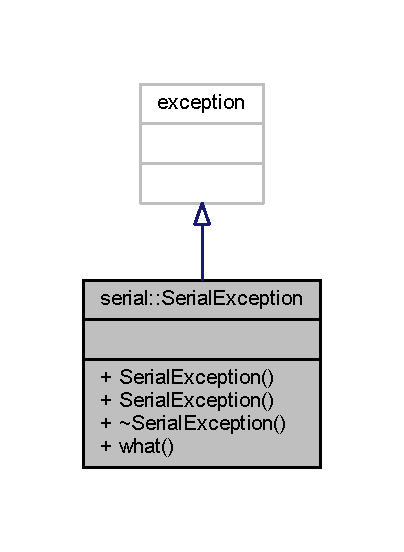
\includegraphics[width=194pt]{classserial_1_1_serial_exception__inherit__graph}
\end{center}
\end{figure}


Collaboration diagram for serial\+:\+:Serial\+Exception\+:\nopagebreak
\begin{figure}[H]
\begin{center}
\leavevmode
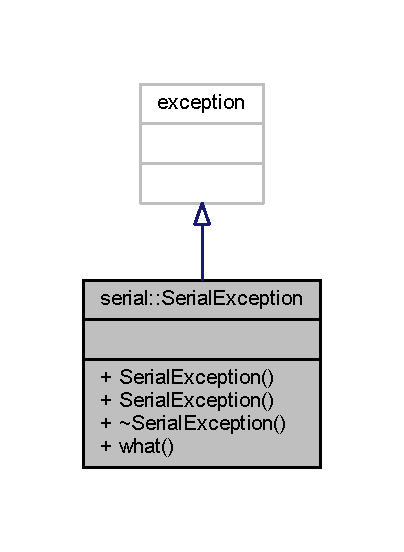
\includegraphics[width=194pt]{classserial_1_1_serial_exception__coll__graph}
\end{center}
\end{figure}
\subsection*{Public Member Functions}
\begin{DoxyCompactItemize}
\item 
\mbox{\hyperlink{classserial_1_1_serial_exception_ab761c0c6e5350bb30f2be40dd6073145}{Serial\+Exception}} (const char $\ast$description)
\item 
\mbox{\hyperlink{classserial_1_1_serial_exception_a6fdfaff3c76d75f1482944ff9ac1cfbe}{Serial\+Exception}} (const \mbox{\hyperlink{classserial_1_1_serial_exception}{Serial\+Exception}} \&other)
\item 
virtual \mbox{\hyperlink{classserial_1_1_serial_exception_a8504adb442f224ec2798e4bd33115fe3}{$\sim$\+Serial\+Exception}} ()  throw ()
\item 
virtual const char $\ast$ \mbox{\hyperlink{classserial_1_1_serial_exception_a8243a4e5c5414834d3ac347c325b961f}{what}} () const  throw ()
\end{DoxyCompactItemize}


\subsection{Constructor \& Destructor Documentation}
\mbox{\Hypertarget{classserial_1_1_serial_exception_ab761c0c6e5350bb30f2be40dd6073145}\label{classserial_1_1_serial_exception_ab761c0c6e5350bb30f2be40dd6073145}} 
\index{serial\+::\+Serial\+Exception@{serial\+::\+Serial\+Exception}!Serial\+Exception@{Serial\+Exception}}
\index{Serial\+Exception@{Serial\+Exception}!serial\+::\+Serial\+Exception@{serial\+::\+Serial\+Exception}}
\subsubsection{\texorpdfstring{Serial\+Exception()}{SerialException()}\hspace{0.1cm}{\footnotesize\ttfamily [1/2]}}
{\footnotesize\ttfamily serial\+::\+Serial\+Exception\+::\+Serial\+Exception (\begin{DoxyParamCaption}\item[{const char $\ast$}]{description }\end{DoxyParamCaption})\hspace{0.3cm}{\ttfamily [inline]}}

\mbox{\Hypertarget{classserial_1_1_serial_exception_a6fdfaff3c76d75f1482944ff9ac1cfbe}\label{classserial_1_1_serial_exception_a6fdfaff3c76d75f1482944ff9ac1cfbe}} 
\index{serial\+::\+Serial\+Exception@{serial\+::\+Serial\+Exception}!Serial\+Exception@{Serial\+Exception}}
\index{Serial\+Exception@{Serial\+Exception}!serial\+::\+Serial\+Exception@{serial\+::\+Serial\+Exception}}
\subsubsection{\texorpdfstring{Serial\+Exception()}{SerialException()}\hspace{0.1cm}{\footnotesize\ttfamily [2/2]}}
{\footnotesize\ttfamily serial\+::\+Serial\+Exception\+::\+Serial\+Exception (\begin{DoxyParamCaption}\item[{const \mbox{\hyperlink{classserial_1_1_serial_exception}{Serial\+Exception}} \&}]{other }\end{DoxyParamCaption})\hspace{0.3cm}{\ttfamily [inline]}}

\mbox{\Hypertarget{classserial_1_1_serial_exception_a8504adb442f224ec2798e4bd33115fe3}\label{classserial_1_1_serial_exception_a8504adb442f224ec2798e4bd33115fe3}} 
\index{serial\+::\+Serial\+Exception@{serial\+::\+Serial\+Exception}!````~Serial\+Exception@{$\sim$\+Serial\+Exception}}
\index{````~Serial\+Exception@{$\sim$\+Serial\+Exception}!serial\+::\+Serial\+Exception@{serial\+::\+Serial\+Exception}}
\subsubsection{\texorpdfstring{$\sim$\+Serial\+Exception()}{~SerialException()}}
{\footnotesize\ttfamily virtual serial\+::\+Serial\+Exception\+::$\sim$\+Serial\+Exception (\begin{DoxyParamCaption}{ }\end{DoxyParamCaption}) throw  ) \hspace{0.3cm}{\ttfamily [inline]}, {\ttfamily [virtual]}}



\subsection{Member Function Documentation}
\mbox{\Hypertarget{classserial_1_1_serial_exception_a8243a4e5c5414834d3ac347c325b961f}\label{classserial_1_1_serial_exception_a8243a4e5c5414834d3ac347c325b961f}} 
\index{serial\+::\+Serial\+Exception@{serial\+::\+Serial\+Exception}!what@{what}}
\index{what@{what}!serial\+::\+Serial\+Exception@{serial\+::\+Serial\+Exception}}
\subsubsection{\texorpdfstring{what()}{what()}}
{\footnotesize\ttfamily virtual const char$\ast$ serial\+::\+Serial\+Exception\+::what (\begin{DoxyParamCaption}{ }\end{DoxyParamCaption}) const throw  ) \hspace{0.3cm}{\ttfamily [inline]}, {\ttfamily [virtual]}}



The documentation for this class was generated from the following file\+:\begin{DoxyCompactItemize}
\item 
C\+:/folders/d/scripts/cpp/\+O\+P\+T3101\+S\+D\+K/\+O\+P\+T3101\+S\+D\+K/\+O\+P\+T3101\+S\+D\+K/serial\+Lib/\mbox{\hyperlink{serial_8h}{serial.\+h}}\end{DoxyCompactItemize}

\hypertarget{classserial_1_1serial_1_1_serial_1_1_serial_impl}{}\section{serial\+:\+:serial\+:\+:Serial\+:\+:Serial\+Impl Class Reference}
\label{classserial_1_1serial_1_1_serial_1_1_serial_impl}\index{serial\+::serial\+::\+Serial\+::\+Serial\+Impl@{serial\+::serial\+::\+Serial\+::\+Serial\+Impl}}


{\ttfamily \#include $<$unix.\+h$>$}



Collaboration diagram for serial\+:\+:serial\+:\+:Serial\+:\+:Serial\+Impl\+:\nopagebreak
\begin{figure}[H]
\begin{center}
\leavevmode
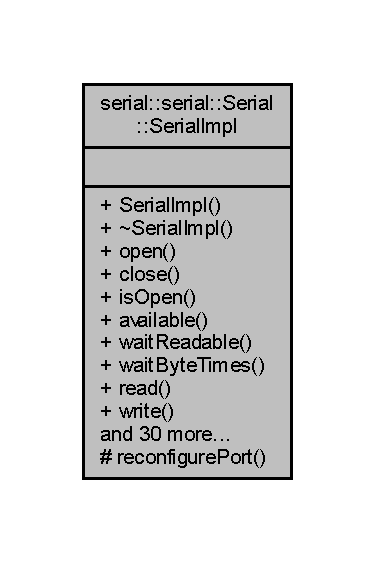
\includegraphics[width=180pt]{classserial_1_1serial_1_1_serial_1_1_serial_impl__coll__graph}
\end{center}
\end{figure}
\subsection*{Public Member Functions}
\begin{DoxyCompactItemize}
\item 
\mbox{\hyperlink{classserial_1_1serial_1_1_serial_1_1_serial_impl_a80885778652ea3c7f7db39ec3f20310c}{Serial\+Impl}} (const string \&port, unsigned long baudrate, \mbox{\hyperlink{namespaceserial_a00b3281fa11cea770c0b0c8a106080f8}{bytesize\+\_\+t}} bytesize, \mbox{\hyperlink{namespaceserial_a8f45d26bf7c9a06659e75b5004a50481}{parity\+\_\+t}} parity, \mbox{\hyperlink{namespaceserial_af5b116611d6628a3aa8f788fdc09f469}{stopbits\+\_\+t}} stopbits, \mbox{\hyperlink{namespaceserial_a93ef57a314b4e562f9eded6c15d34351}{flowcontrol\+\_\+t}} flowcontrol)
\item 
virtual \mbox{\hyperlink{classserial_1_1serial_1_1_serial_1_1_serial_impl_af9f0a13782d7870cf66a49001dcc64e7}{$\sim$\+Serial\+Impl}} ()
\item 
void \mbox{\hyperlink{classserial_1_1serial_1_1_serial_1_1_serial_impl_a279801879f609e1845e3e730f5651aa2}{open}} ()
\item 
void \mbox{\hyperlink{classserial_1_1serial_1_1_serial_1_1_serial_impl_a2608096ba0d17127b17484fc9481833a}{close}} ()
\item 
bool \mbox{\hyperlink{classserial_1_1serial_1_1_serial_1_1_serial_impl_a78f28bc8e63ef24aa805178571f4b384}{is\+Open}} () const
\item 
size\+\_\+t \mbox{\hyperlink{classserial_1_1serial_1_1_serial_1_1_serial_impl_aecd5e068c21b076bcf161f7bf7f415f5}{available}} ()
\item 
bool \mbox{\hyperlink{classserial_1_1serial_1_1_serial_1_1_serial_impl_a4722f7080b15d12a4e00672858c5f0e8}{wait\+Readable}} (uint32\+\_\+t timeout)
\item 
void \mbox{\hyperlink{classserial_1_1serial_1_1_serial_1_1_serial_impl_a039703d806b1c8db071da9a04cf63446}{wait\+Byte\+Times}} (size\+\_\+t count)
\item 
size\+\_\+t \mbox{\hyperlink{classserial_1_1serial_1_1_serial_1_1_serial_impl_ada61c83884f0f6350874fc32e640cbac}{read}} (uint8\+\_\+t $\ast$buf, size\+\_\+t size=1)
\item 
size\+\_\+t \mbox{\hyperlink{classserial_1_1serial_1_1_serial_1_1_serial_impl_a89b50df2562176fd250413833d636d0a}{write}} (const uint8\+\_\+t $\ast$data, size\+\_\+t length)
\item 
void \mbox{\hyperlink{classserial_1_1serial_1_1_serial_1_1_serial_impl_afe873a403bcca3956437d95aa55c4d06}{flush}} ()
\item 
void \mbox{\hyperlink{classserial_1_1serial_1_1_serial_1_1_serial_impl_a0b4ef99a4b44c3ef153ec7c4802ff194}{flush\+Input}} ()
\item 
void \mbox{\hyperlink{classserial_1_1serial_1_1_serial_1_1_serial_impl_ac61932385ea2ce645192e1539349500b}{flush\+Output}} ()
\item 
void \mbox{\hyperlink{classserial_1_1serial_1_1_serial_1_1_serial_impl_a6a1abcf6f4b94c7f3d7753c3f2dab91a}{send\+Break}} (int duration)
\item 
void \mbox{\hyperlink{classserial_1_1serial_1_1_serial_1_1_serial_impl_a4e439ed9ab4e38fb64bba2d49b814179}{set\+Break}} (bool level)
\item 
void \mbox{\hyperlink{classserial_1_1serial_1_1_serial_1_1_serial_impl_a7faf4ef9a0f1b13c9155a4cae1e0ace9}{set\+R\+TS}} (bool level)
\item 
void \mbox{\hyperlink{classserial_1_1serial_1_1_serial_1_1_serial_impl_a94cdd2aad19377a0ec435bb6241b98a8}{set\+D\+TR}} (bool level)
\item 
bool \mbox{\hyperlink{classserial_1_1serial_1_1_serial_1_1_serial_impl_a09f1dcb8e32cb64188daaf8ac0d40215}{wait\+For\+Change}} ()
\item 
bool \mbox{\hyperlink{classserial_1_1serial_1_1_serial_1_1_serial_impl_afbfd566cd435f7881826fb0a2f74f746}{get\+C\+TS}} ()
\item 
bool \mbox{\hyperlink{classserial_1_1serial_1_1_serial_1_1_serial_impl_ae07e012e3630c51baf1b8c7c37dd79a5}{get\+D\+SR}} ()
\item 
bool \mbox{\hyperlink{classserial_1_1serial_1_1_serial_1_1_serial_impl_a4b9e1b75dce29e8ed4fa62b389510ae5}{get\+RI}} ()
\item 
bool \mbox{\hyperlink{classserial_1_1serial_1_1_serial_1_1_serial_impl_a9d402e28513e22613658b31e13b76802}{get\+CD}} ()
\item 
void \mbox{\hyperlink{classserial_1_1serial_1_1_serial_1_1_serial_impl_aa3b4c490f3246a506dd29135553ecd64}{set\+Port}} (const string \&port)
\item 
string \mbox{\hyperlink{classserial_1_1serial_1_1_serial_1_1_serial_impl_aae10cc0beaa3fc5b9d88c53c976edf1a}{get\+Port}} () const
\item 
void \mbox{\hyperlink{classserial_1_1serial_1_1_serial_1_1_serial_impl_a22cc09f7e828c54631392dc69e3737d3}{set\+Timeout}} (\mbox{\hyperlink{structserial_1_1_timeout}{Timeout}} \&timeout)
\item 
\mbox{\hyperlink{structserial_1_1_timeout}{Timeout}} \mbox{\hyperlink{classserial_1_1serial_1_1_serial_1_1_serial_impl_ac83d791d7720e05499c2dbe6cb3f4ae2}{get\+Timeout}} () const
\item 
void \mbox{\hyperlink{classserial_1_1serial_1_1_serial_1_1_serial_impl_ad57c0c497d487c2f2115168f60eda146}{set\+Baudrate}} (unsigned long baudrate)
\item 
unsigned long \mbox{\hyperlink{classserial_1_1serial_1_1_serial_1_1_serial_impl_a55c2c091aff0bc22c3d770fa528e0f17}{get\+Baudrate}} () const
\item 
void \mbox{\hyperlink{classserial_1_1serial_1_1_serial_1_1_serial_impl_aa788845b977360851810f07a07b340a7}{set\+Bytesize}} (\mbox{\hyperlink{namespaceserial_a00b3281fa11cea770c0b0c8a106080f8}{bytesize\+\_\+t}} bytesize)
\item 
\mbox{\hyperlink{namespaceserial_a00b3281fa11cea770c0b0c8a106080f8}{bytesize\+\_\+t}} \mbox{\hyperlink{classserial_1_1serial_1_1_serial_1_1_serial_impl_a3091d3840db8f1281bbbce78da13eaf7}{get\+Bytesize}} () const
\item 
void \mbox{\hyperlink{classserial_1_1serial_1_1_serial_1_1_serial_impl_a7859629014393110fc76a55f1d956c3f}{set\+Parity}} (\mbox{\hyperlink{namespaceserial_a8f45d26bf7c9a06659e75b5004a50481}{parity\+\_\+t}} parity)
\item 
\mbox{\hyperlink{namespaceserial_a8f45d26bf7c9a06659e75b5004a50481}{parity\+\_\+t}} \mbox{\hyperlink{classserial_1_1serial_1_1_serial_1_1_serial_impl_a3dd2675e55de5cfd2be9fd23268bf765}{get\+Parity}} () const
\item 
void \mbox{\hyperlink{classserial_1_1serial_1_1_serial_1_1_serial_impl_a23f31163c4c1b4aa488a7c7204ddec17}{set\+Stopbits}} (\mbox{\hyperlink{namespaceserial_af5b116611d6628a3aa8f788fdc09f469}{stopbits\+\_\+t}} stopbits)
\item 
\mbox{\hyperlink{namespaceserial_af5b116611d6628a3aa8f788fdc09f469}{stopbits\+\_\+t}} \mbox{\hyperlink{classserial_1_1serial_1_1_serial_1_1_serial_impl_adc56daf989276c47cff8b10564025476}{get\+Stopbits}} () const
\item 
void \mbox{\hyperlink{classserial_1_1serial_1_1_serial_1_1_serial_impl_abe20c54b814d70e1e0deaa8d3472babe}{set\+Flowcontrol}} (\mbox{\hyperlink{namespaceserial_a93ef57a314b4e562f9eded6c15d34351}{flowcontrol\+\_\+t}} flowcontrol)
\item 
\mbox{\hyperlink{namespaceserial_a93ef57a314b4e562f9eded6c15d34351}{flowcontrol\+\_\+t}} \mbox{\hyperlink{classserial_1_1serial_1_1_serial_1_1_serial_impl_aaa2af4d3b08a0f40da7527af419ec903}{get\+Flowcontrol}} () const
\item 
void \mbox{\hyperlink{classserial_1_1serial_1_1_serial_1_1_serial_impl_a284eeedc3dd686ecef0fdcfd83bebc54}{read\+Lock}} ()
\item 
void \mbox{\hyperlink{classserial_1_1serial_1_1_serial_1_1_serial_impl_ab6533e884ba609a1dd6a88b7964d8b52}{read\+Unlock}} ()
\item 
void \mbox{\hyperlink{classserial_1_1serial_1_1_serial_1_1_serial_impl_a2905e50e9082a757bfafc03356e318ed}{write\+Lock}} ()
\item 
void \mbox{\hyperlink{classserial_1_1serial_1_1_serial_1_1_serial_impl_adaec2b322f0b0793929da24f5bf09949}{write\+Unlock}} ()
\end{DoxyCompactItemize}
\subsection*{Protected Member Functions}
\begin{DoxyCompactItemize}
\item 
void \mbox{\hyperlink{classserial_1_1serial_1_1_serial_1_1_serial_impl_ad006a2392150daddfa43ae288259c07d}{reconfigure\+Port}} ()
\end{DoxyCompactItemize}


\subsection{Constructor \& Destructor Documentation}
\mbox{\Hypertarget{classserial_1_1serial_1_1_serial_1_1_serial_impl_a80885778652ea3c7f7db39ec3f20310c}\label{classserial_1_1serial_1_1_serial_1_1_serial_impl_a80885778652ea3c7f7db39ec3f20310c}} 
\index{serial\+::serial\+::\+Serial\+::\+Serial\+Impl@{serial\+::serial\+::\+Serial\+::\+Serial\+Impl}!Serial\+Impl@{Serial\+Impl}}
\index{Serial\+Impl@{Serial\+Impl}!serial\+::serial\+::\+Serial\+::\+Serial\+Impl@{serial\+::serial\+::\+Serial\+::\+Serial\+Impl}}
\subsubsection{\texorpdfstring{Serial\+Impl()}{SerialImpl()}}
{\footnotesize\ttfamily Serial\+::\+Serial\+Impl\+::\+Serial\+Impl (\begin{DoxyParamCaption}\item[{const string \&}]{port,  }\item[{unsigned long}]{baudrate,  }\item[{\mbox{\hyperlink{namespaceserial_a00b3281fa11cea770c0b0c8a106080f8}{bytesize\+\_\+t}}}]{bytesize,  }\item[{\mbox{\hyperlink{namespaceserial_a8f45d26bf7c9a06659e75b5004a50481}{parity\+\_\+t}}}]{parity,  }\item[{\mbox{\hyperlink{namespaceserial_af5b116611d6628a3aa8f788fdc09f469}{stopbits\+\_\+t}}}]{stopbits,  }\item[{\mbox{\hyperlink{namespaceserial_a93ef57a314b4e562f9eded6c15d34351}{flowcontrol\+\_\+t}}}]{flowcontrol }\end{DoxyParamCaption})}

\mbox{\Hypertarget{classserial_1_1serial_1_1_serial_1_1_serial_impl_af9f0a13782d7870cf66a49001dcc64e7}\label{classserial_1_1serial_1_1_serial_1_1_serial_impl_af9f0a13782d7870cf66a49001dcc64e7}} 
\index{serial\+::serial\+::\+Serial\+::\+Serial\+Impl@{serial\+::serial\+::\+Serial\+::\+Serial\+Impl}!````~Serial\+Impl@{$\sim$\+Serial\+Impl}}
\index{````~Serial\+Impl@{$\sim$\+Serial\+Impl}!serial\+::serial\+::\+Serial\+::\+Serial\+Impl@{serial\+::serial\+::\+Serial\+::\+Serial\+Impl}}
\subsubsection{\texorpdfstring{$\sim$\+Serial\+Impl()}{~SerialImpl()}}
{\footnotesize\ttfamily Serial\+::\+Serial\+Impl\+::$\sim$\+Serial\+Impl (\begin{DoxyParamCaption}{ }\end{DoxyParamCaption})\hspace{0.3cm}{\ttfamily [virtual]}}



\subsection{Member Function Documentation}
\mbox{\Hypertarget{classserial_1_1serial_1_1_serial_1_1_serial_impl_aecd5e068c21b076bcf161f7bf7f415f5}\label{classserial_1_1serial_1_1_serial_1_1_serial_impl_aecd5e068c21b076bcf161f7bf7f415f5}} 
\index{serial\+::serial\+::\+Serial\+::\+Serial\+Impl@{serial\+::serial\+::\+Serial\+::\+Serial\+Impl}!available@{available}}
\index{available@{available}!serial\+::serial\+::\+Serial\+::\+Serial\+Impl@{serial\+::serial\+::\+Serial\+::\+Serial\+Impl}}
\subsubsection{\texorpdfstring{available()}{available()}}
{\footnotesize\ttfamily size\+\_\+t Serial\+::\+Serial\+Impl\+::available (\begin{DoxyParamCaption}{ }\end{DoxyParamCaption})}

\mbox{\Hypertarget{classserial_1_1serial_1_1_serial_1_1_serial_impl_a2608096ba0d17127b17484fc9481833a}\label{classserial_1_1serial_1_1_serial_1_1_serial_impl_a2608096ba0d17127b17484fc9481833a}} 
\index{serial\+::serial\+::\+Serial\+::\+Serial\+Impl@{serial\+::serial\+::\+Serial\+::\+Serial\+Impl}!close@{close}}
\index{close@{close}!serial\+::serial\+::\+Serial\+::\+Serial\+Impl@{serial\+::serial\+::\+Serial\+::\+Serial\+Impl}}
\subsubsection{\texorpdfstring{close()}{close()}}
{\footnotesize\ttfamily void Serial\+::\+Serial\+Impl\+::close (\begin{DoxyParamCaption}{ }\end{DoxyParamCaption})}

\mbox{\Hypertarget{classserial_1_1serial_1_1_serial_1_1_serial_impl_afe873a403bcca3956437d95aa55c4d06}\label{classserial_1_1serial_1_1_serial_1_1_serial_impl_afe873a403bcca3956437d95aa55c4d06}} 
\index{serial\+::serial\+::\+Serial\+::\+Serial\+Impl@{serial\+::serial\+::\+Serial\+::\+Serial\+Impl}!flush@{flush}}
\index{flush@{flush}!serial\+::serial\+::\+Serial\+::\+Serial\+Impl@{serial\+::serial\+::\+Serial\+::\+Serial\+Impl}}
\subsubsection{\texorpdfstring{flush()}{flush()}}
{\footnotesize\ttfamily void Serial\+::\+Serial\+Impl\+::flush (\begin{DoxyParamCaption}{ }\end{DoxyParamCaption})}

\mbox{\Hypertarget{classserial_1_1serial_1_1_serial_1_1_serial_impl_a0b4ef99a4b44c3ef153ec7c4802ff194}\label{classserial_1_1serial_1_1_serial_1_1_serial_impl_a0b4ef99a4b44c3ef153ec7c4802ff194}} 
\index{serial\+::serial\+::\+Serial\+::\+Serial\+Impl@{serial\+::serial\+::\+Serial\+::\+Serial\+Impl}!flush\+Input@{flush\+Input}}
\index{flush\+Input@{flush\+Input}!serial\+::serial\+::\+Serial\+::\+Serial\+Impl@{serial\+::serial\+::\+Serial\+::\+Serial\+Impl}}
\subsubsection{\texorpdfstring{flush\+Input()}{flushInput()}}
{\footnotesize\ttfamily void Serial\+::\+Serial\+Impl\+::flush\+Input (\begin{DoxyParamCaption}{ }\end{DoxyParamCaption})}

\mbox{\Hypertarget{classserial_1_1serial_1_1_serial_1_1_serial_impl_ac61932385ea2ce645192e1539349500b}\label{classserial_1_1serial_1_1_serial_1_1_serial_impl_ac61932385ea2ce645192e1539349500b}} 
\index{serial\+::serial\+::\+Serial\+::\+Serial\+Impl@{serial\+::serial\+::\+Serial\+::\+Serial\+Impl}!flush\+Output@{flush\+Output}}
\index{flush\+Output@{flush\+Output}!serial\+::serial\+::\+Serial\+::\+Serial\+Impl@{serial\+::serial\+::\+Serial\+::\+Serial\+Impl}}
\subsubsection{\texorpdfstring{flush\+Output()}{flushOutput()}}
{\footnotesize\ttfamily void Serial\+::\+Serial\+Impl\+::flush\+Output (\begin{DoxyParamCaption}{ }\end{DoxyParamCaption})}

\mbox{\Hypertarget{classserial_1_1serial_1_1_serial_1_1_serial_impl_a55c2c091aff0bc22c3d770fa528e0f17}\label{classserial_1_1serial_1_1_serial_1_1_serial_impl_a55c2c091aff0bc22c3d770fa528e0f17}} 
\index{serial\+::serial\+::\+Serial\+::\+Serial\+Impl@{serial\+::serial\+::\+Serial\+::\+Serial\+Impl}!get\+Baudrate@{get\+Baudrate}}
\index{get\+Baudrate@{get\+Baudrate}!serial\+::serial\+::\+Serial\+::\+Serial\+Impl@{serial\+::serial\+::\+Serial\+::\+Serial\+Impl}}
\subsubsection{\texorpdfstring{get\+Baudrate()}{getBaudrate()}}
{\footnotesize\ttfamily unsigned long Serial\+::\+Serial\+Impl\+::get\+Baudrate (\begin{DoxyParamCaption}{ }\end{DoxyParamCaption}) const}

\mbox{\Hypertarget{classserial_1_1serial_1_1_serial_1_1_serial_impl_a3091d3840db8f1281bbbce78da13eaf7}\label{classserial_1_1serial_1_1_serial_1_1_serial_impl_a3091d3840db8f1281bbbce78da13eaf7}} 
\index{serial\+::serial\+::\+Serial\+::\+Serial\+Impl@{serial\+::serial\+::\+Serial\+::\+Serial\+Impl}!get\+Bytesize@{get\+Bytesize}}
\index{get\+Bytesize@{get\+Bytesize}!serial\+::serial\+::\+Serial\+::\+Serial\+Impl@{serial\+::serial\+::\+Serial\+::\+Serial\+Impl}}
\subsubsection{\texorpdfstring{get\+Bytesize()}{getBytesize()}}
{\footnotesize\ttfamily \mbox{\hyperlink{namespaceserial_a00b3281fa11cea770c0b0c8a106080f8}{serial\+::bytesize\+\_\+t}} Serial\+::\+Serial\+Impl\+::get\+Bytesize (\begin{DoxyParamCaption}{ }\end{DoxyParamCaption}) const}

\mbox{\Hypertarget{classserial_1_1serial_1_1_serial_1_1_serial_impl_a9d402e28513e22613658b31e13b76802}\label{classserial_1_1serial_1_1_serial_1_1_serial_impl_a9d402e28513e22613658b31e13b76802}} 
\index{serial\+::serial\+::\+Serial\+::\+Serial\+Impl@{serial\+::serial\+::\+Serial\+::\+Serial\+Impl}!get\+CD@{get\+CD}}
\index{get\+CD@{get\+CD}!serial\+::serial\+::\+Serial\+::\+Serial\+Impl@{serial\+::serial\+::\+Serial\+::\+Serial\+Impl}}
\subsubsection{\texorpdfstring{get\+C\+D()}{getCD()}}
{\footnotesize\ttfamily bool Serial\+::\+Serial\+Impl\+::get\+CD (\begin{DoxyParamCaption}{ }\end{DoxyParamCaption})}

\mbox{\Hypertarget{classserial_1_1serial_1_1_serial_1_1_serial_impl_afbfd566cd435f7881826fb0a2f74f746}\label{classserial_1_1serial_1_1_serial_1_1_serial_impl_afbfd566cd435f7881826fb0a2f74f746}} 
\index{serial\+::serial\+::\+Serial\+::\+Serial\+Impl@{serial\+::serial\+::\+Serial\+::\+Serial\+Impl}!get\+C\+TS@{get\+C\+TS}}
\index{get\+C\+TS@{get\+C\+TS}!serial\+::serial\+::\+Serial\+::\+Serial\+Impl@{serial\+::serial\+::\+Serial\+::\+Serial\+Impl}}
\subsubsection{\texorpdfstring{get\+C\+T\+S()}{getCTS()}}
{\footnotesize\ttfamily bool Serial\+::\+Serial\+Impl\+::get\+C\+TS (\begin{DoxyParamCaption}{ }\end{DoxyParamCaption})}

\mbox{\Hypertarget{classserial_1_1serial_1_1_serial_1_1_serial_impl_ae07e012e3630c51baf1b8c7c37dd79a5}\label{classserial_1_1serial_1_1_serial_1_1_serial_impl_ae07e012e3630c51baf1b8c7c37dd79a5}} 
\index{serial\+::serial\+::\+Serial\+::\+Serial\+Impl@{serial\+::serial\+::\+Serial\+::\+Serial\+Impl}!get\+D\+SR@{get\+D\+SR}}
\index{get\+D\+SR@{get\+D\+SR}!serial\+::serial\+::\+Serial\+::\+Serial\+Impl@{serial\+::serial\+::\+Serial\+::\+Serial\+Impl}}
\subsubsection{\texorpdfstring{get\+D\+S\+R()}{getDSR()}}
{\footnotesize\ttfamily bool Serial\+::\+Serial\+Impl\+::get\+D\+SR (\begin{DoxyParamCaption}{ }\end{DoxyParamCaption})}

\mbox{\Hypertarget{classserial_1_1serial_1_1_serial_1_1_serial_impl_aaa2af4d3b08a0f40da7527af419ec903}\label{classserial_1_1serial_1_1_serial_1_1_serial_impl_aaa2af4d3b08a0f40da7527af419ec903}} 
\index{serial\+::serial\+::\+Serial\+::\+Serial\+Impl@{serial\+::serial\+::\+Serial\+::\+Serial\+Impl}!get\+Flowcontrol@{get\+Flowcontrol}}
\index{get\+Flowcontrol@{get\+Flowcontrol}!serial\+::serial\+::\+Serial\+::\+Serial\+Impl@{serial\+::serial\+::\+Serial\+::\+Serial\+Impl}}
\subsubsection{\texorpdfstring{get\+Flowcontrol()}{getFlowcontrol()}}
{\footnotesize\ttfamily \mbox{\hyperlink{namespaceserial_a93ef57a314b4e562f9eded6c15d34351}{serial\+::flowcontrol\+\_\+t}} Serial\+::\+Serial\+Impl\+::get\+Flowcontrol (\begin{DoxyParamCaption}{ }\end{DoxyParamCaption}) const}

\mbox{\Hypertarget{classserial_1_1serial_1_1_serial_1_1_serial_impl_a3dd2675e55de5cfd2be9fd23268bf765}\label{classserial_1_1serial_1_1_serial_1_1_serial_impl_a3dd2675e55de5cfd2be9fd23268bf765}} 
\index{serial\+::serial\+::\+Serial\+::\+Serial\+Impl@{serial\+::serial\+::\+Serial\+::\+Serial\+Impl}!get\+Parity@{get\+Parity}}
\index{get\+Parity@{get\+Parity}!serial\+::serial\+::\+Serial\+::\+Serial\+Impl@{serial\+::serial\+::\+Serial\+::\+Serial\+Impl}}
\subsubsection{\texorpdfstring{get\+Parity()}{getParity()}}
{\footnotesize\ttfamily \mbox{\hyperlink{namespaceserial_a8f45d26bf7c9a06659e75b5004a50481}{serial\+::parity\+\_\+t}} Serial\+::\+Serial\+Impl\+::get\+Parity (\begin{DoxyParamCaption}{ }\end{DoxyParamCaption}) const}

\mbox{\Hypertarget{classserial_1_1serial_1_1_serial_1_1_serial_impl_aae10cc0beaa3fc5b9d88c53c976edf1a}\label{classserial_1_1serial_1_1_serial_1_1_serial_impl_aae10cc0beaa3fc5b9d88c53c976edf1a}} 
\index{serial\+::serial\+::\+Serial\+::\+Serial\+Impl@{serial\+::serial\+::\+Serial\+::\+Serial\+Impl}!get\+Port@{get\+Port}}
\index{get\+Port@{get\+Port}!serial\+::serial\+::\+Serial\+::\+Serial\+Impl@{serial\+::serial\+::\+Serial\+::\+Serial\+Impl}}
\subsubsection{\texorpdfstring{get\+Port()}{getPort()}}
{\footnotesize\ttfamily string Serial\+::\+Serial\+Impl\+::get\+Port (\begin{DoxyParamCaption}{ }\end{DoxyParamCaption}) const}

\mbox{\Hypertarget{classserial_1_1serial_1_1_serial_1_1_serial_impl_a4b9e1b75dce29e8ed4fa62b389510ae5}\label{classserial_1_1serial_1_1_serial_1_1_serial_impl_a4b9e1b75dce29e8ed4fa62b389510ae5}} 
\index{serial\+::serial\+::\+Serial\+::\+Serial\+Impl@{serial\+::serial\+::\+Serial\+::\+Serial\+Impl}!get\+RI@{get\+RI}}
\index{get\+RI@{get\+RI}!serial\+::serial\+::\+Serial\+::\+Serial\+Impl@{serial\+::serial\+::\+Serial\+::\+Serial\+Impl}}
\subsubsection{\texorpdfstring{get\+R\+I()}{getRI()}}
{\footnotesize\ttfamily bool Serial\+::\+Serial\+Impl\+::get\+RI (\begin{DoxyParamCaption}{ }\end{DoxyParamCaption})}

\mbox{\Hypertarget{classserial_1_1serial_1_1_serial_1_1_serial_impl_adc56daf989276c47cff8b10564025476}\label{classserial_1_1serial_1_1_serial_1_1_serial_impl_adc56daf989276c47cff8b10564025476}} 
\index{serial\+::serial\+::\+Serial\+::\+Serial\+Impl@{serial\+::serial\+::\+Serial\+::\+Serial\+Impl}!get\+Stopbits@{get\+Stopbits}}
\index{get\+Stopbits@{get\+Stopbits}!serial\+::serial\+::\+Serial\+::\+Serial\+Impl@{serial\+::serial\+::\+Serial\+::\+Serial\+Impl}}
\subsubsection{\texorpdfstring{get\+Stopbits()}{getStopbits()}}
{\footnotesize\ttfamily \mbox{\hyperlink{namespaceserial_af5b116611d6628a3aa8f788fdc09f469}{serial\+::stopbits\+\_\+t}} Serial\+::\+Serial\+Impl\+::get\+Stopbits (\begin{DoxyParamCaption}{ }\end{DoxyParamCaption}) const}

\mbox{\Hypertarget{classserial_1_1serial_1_1_serial_1_1_serial_impl_ac83d791d7720e05499c2dbe6cb3f4ae2}\label{classserial_1_1serial_1_1_serial_1_1_serial_impl_ac83d791d7720e05499c2dbe6cb3f4ae2}} 
\index{serial\+::serial\+::\+Serial\+::\+Serial\+Impl@{serial\+::serial\+::\+Serial\+::\+Serial\+Impl}!get\+Timeout@{get\+Timeout}}
\index{get\+Timeout@{get\+Timeout}!serial\+::serial\+::\+Serial\+::\+Serial\+Impl@{serial\+::serial\+::\+Serial\+::\+Serial\+Impl}}
\subsubsection{\texorpdfstring{get\+Timeout()}{getTimeout()}}
{\footnotesize\ttfamily \mbox{\hyperlink{structserial_1_1_timeout}{serial\+::\+Timeout}} Serial\+::\+Serial\+Impl\+::get\+Timeout (\begin{DoxyParamCaption}{ }\end{DoxyParamCaption}) const}

\mbox{\Hypertarget{classserial_1_1serial_1_1_serial_1_1_serial_impl_a78f28bc8e63ef24aa805178571f4b384}\label{classserial_1_1serial_1_1_serial_1_1_serial_impl_a78f28bc8e63ef24aa805178571f4b384}} 
\index{serial\+::serial\+::\+Serial\+::\+Serial\+Impl@{serial\+::serial\+::\+Serial\+::\+Serial\+Impl}!is\+Open@{is\+Open}}
\index{is\+Open@{is\+Open}!serial\+::serial\+::\+Serial\+::\+Serial\+Impl@{serial\+::serial\+::\+Serial\+::\+Serial\+Impl}}
\subsubsection{\texorpdfstring{is\+Open()}{isOpen()}}
{\footnotesize\ttfamily bool Serial\+::\+Serial\+Impl\+::is\+Open (\begin{DoxyParamCaption}{ }\end{DoxyParamCaption}) const}

\mbox{\Hypertarget{classserial_1_1serial_1_1_serial_1_1_serial_impl_a279801879f609e1845e3e730f5651aa2}\label{classserial_1_1serial_1_1_serial_1_1_serial_impl_a279801879f609e1845e3e730f5651aa2}} 
\index{serial\+::serial\+::\+Serial\+::\+Serial\+Impl@{serial\+::serial\+::\+Serial\+::\+Serial\+Impl}!open@{open}}
\index{open@{open}!serial\+::serial\+::\+Serial\+::\+Serial\+Impl@{serial\+::serial\+::\+Serial\+::\+Serial\+Impl}}
\subsubsection{\texorpdfstring{open()}{open()}}
{\footnotesize\ttfamily void Serial\+::\+Serial\+Impl\+::open (\begin{DoxyParamCaption}{ }\end{DoxyParamCaption})}

\mbox{\Hypertarget{classserial_1_1serial_1_1_serial_1_1_serial_impl_ada61c83884f0f6350874fc32e640cbac}\label{classserial_1_1serial_1_1_serial_1_1_serial_impl_ada61c83884f0f6350874fc32e640cbac}} 
\index{serial\+::serial\+::\+Serial\+::\+Serial\+Impl@{serial\+::serial\+::\+Serial\+::\+Serial\+Impl}!read@{read}}
\index{read@{read}!serial\+::serial\+::\+Serial\+::\+Serial\+Impl@{serial\+::serial\+::\+Serial\+::\+Serial\+Impl}}
\subsubsection{\texorpdfstring{read()}{read()}}
{\footnotesize\ttfamily size\+\_\+t Serial\+::\+Serial\+Impl\+::read (\begin{DoxyParamCaption}\item[{uint8\+\_\+t $\ast$}]{buf,  }\item[{size\+\_\+t}]{size = {\ttfamily 1} }\end{DoxyParamCaption})}

\mbox{\Hypertarget{classserial_1_1serial_1_1_serial_1_1_serial_impl_a284eeedc3dd686ecef0fdcfd83bebc54}\label{classserial_1_1serial_1_1_serial_1_1_serial_impl_a284eeedc3dd686ecef0fdcfd83bebc54}} 
\index{serial\+::serial\+::\+Serial\+::\+Serial\+Impl@{serial\+::serial\+::\+Serial\+::\+Serial\+Impl}!read\+Lock@{read\+Lock}}
\index{read\+Lock@{read\+Lock}!serial\+::serial\+::\+Serial\+::\+Serial\+Impl@{serial\+::serial\+::\+Serial\+::\+Serial\+Impl}}
\subsubsection{\texorpdfstring{read\+Lock()}{readLock()}}
{\footnotesize\ttfamily void Serial\+::\+Serial\+Impl\+::read\+Lock (\begin{DoxyParamCaption}{ }\end{DoxyParamCaption})}

\mbox{\Hypertarget{classserial_1_1serial_1_1_serial_1_1_serial_impl_ab6533e884ba609a1dd6a88b7964d8b52}\label{classserial_1_1serial_1_1_serial_1_1_serial_impl_ab6533e884ba609a1dd6a88b7964d8b52}} 
\index{serial\+::serial\+::\+Serial\+::\+Serial\+Impl@{serial\+::serial\+::\+Serial\+::\+Serial\+Impl}!read\+Unlock@{read\+Unlock}}
\index{read\+Unlock@{read\+Unlock}!serial\+::serial\+::\+Serial\+::\+Serial\+Impl@{serial\+::serial\+::\+Serial\+::\+Serial\+Impl}}
\subsubsection{\texorpdfstring{read\+Unlock()}{readUnlock()}}
{\footnotesize\ttfamily void Serial\+::\+Serial\+Impl\+::read\+Unlock (\begin{DoxyParamCaption}{ }\end{DoxyParamCaption})}

\mbox{\Hypertarget{classserial_1_1serial_1_1_serial_1_1_serial_impl_ad006a2392150daddfa43ae288259c07d}\label{classserial_1_1serial_1_1_serial_1_1_serial_impl_ad006a2392150daddfa43ae288259c07d}} 
\index{serial\+::serial\+::\+Serial\+::\+Serial\+Impl@{serial\+::serial\+::\+Serial\+::\+Serial\+Impl}!reconfigure\+Port@{reconfigure\+Port}}
\index{reconfigure\+Port@{reconfigure\+Port}!serial\+::serial\+::\+Serial\+::\+Serial\+Impl@{serial\+::serial\+::\+Serial\+::\+Serial\+Impl}}
\subsubsection{\texorpdfstring{reconfigure\+Port()}{reconfigurePort()}}
{\footnotesize\ttfamily void Serial\+::\+Serial\+Impl\+::reconfigure\+Port (\begin{DoxyParamCaption}{ }\end{DoxyParamCaption})\hspace{0.3cm}{\ttfamily [protected]}}

\mbox{\Hypertarget{classserial_1_1serial_1_1_serial_1_1_serial_impl_a6a1abcf6f4b94c7f3d7753c3f2dab91a}\label{classserial_1_1serial_1_1_serial_1_1_serial_impl_a6a1abcf6f4b94c7f3d7753c3f2dab91a}} 
\index{serial\+::serial\+::\+Serial\+::\+Serial\+Impl@{serial\+::serial\+::\+Serial\+::\+Serial\+Impl}!send\+Break@{send\+Break}}
\index{send\+Break@{send\+Break}!serial\+::serial\+::\+Serial\+::\+Serial\+Impl@{serial\+::serial\+::\+Serial\+::\+Serial\+Impl}}
\subsubsection{\texorpdfstring{send\+Break()}{sendBreak()}}
{\footnotesize\ttfamily void Serial\+::\+Serial\+Impl\+::send\+Break (\begin{DoxyParamCaption}\item[{int}]{duration }\end{DoxyParamCaption})}

\mbox{\Hypertarget{classserial_1_1serial_1_1_serial_1_1_serial_impl_ad57c0c497d487c2f2115168f60eda146}\label{classserial_1_1serial_1_1_serial_1_1_serial_impl_ad57c0c497d487c2f2115168f60eda146}} 
\index{serial\+::serial\+::\+Serial\+::\+Serial\+Impl@{serial\+::serial\+::\+Serial\+::\+Serial\+Impl}!set\+Baudrate@{set\+Baudrate}}
\index{set\+Baudrate@{set\+Baudrate}!serial\+::serial\+::\+Serial\+::\+Serial\+Impl@{serial\+::serial\+::\+Serial\+::\+Serial\+Impl}}
\subsubsection{\texorpdfstring{set\+Baudrate()}{setBaudrate()}}
{\footnotesize\ttfamily void Serial\+::\+Serial\+Impl\+::set\+Baudrate (\begin{DoxyParamCaption}\item[{unsigned long}]{baudrate }\end{DoxyParamCaption})}

\mbox{\Hypertarget{classserial_1_1serial_1_1_serial_1_1_serial_impl_a4e439ed9ab4e38fb64bba2d49b814179}\label{classserial_1_1serial_1_1_serial_1_1_serial_impl_a4e439ed9ab4e38fb64bba2d49b814179}} 
\index{serial\+::serial\+::\+Serial\+::\+Serial\+Impl@{serial\+::serial\+::\+Serial\+::\+Serial\+Impl}!set\+Break@{set\+Break}}
\index{set\+Break@{set\+Break}!serial\+::serial\+::\+Serial\+::\+Serial\+Impl@{serial\+::serial\+::\+Serial\+::\+Serial\+Impl}}
\subsubsection{\texorpdfstring{set\+Break()}{setBreak()}}
{\footnotesize\ttfamily void Serial\+::\+Serial\+Impl\+::set\+Break (\begin{DoxyParamCaption}\item[{bool}]{level }\end{DoxyParamCaption})}

\mbox{\Hypertarget{classserial_1_1serial_1_1_serial_1_1_serial_impl_aa788845b977360851810f07a07b340a7}\label{classserial_1_1serial_1_1_serial_1_1_serial_impl_aa788845b977360851810f07a07b340a7}} 
\index{serial\+::serial\+::\+Serial\+::\+Serial\+Impl@{serial\+::serial\+::\+Serial\+::\+Serial\+Impl}!set\+Bytesize@{set\+Bytesize}}
\index{set\+Bytesize@{set\+Bytesize}!serial\+::serial\+::\+Serial\+::\+Serial\+Impl@{serial\+::serial\+::\+Serial\+::\+Serial\+Impl}}
\subsubsection{\texorpdfstring{set\+Bytesize()}{setBytesize()}}
{\footnotesize\ttfamily void Serial\+::\+Serial\+Impl\+::set\+Bytesize (\begin{DoxyParamCaption}\item[{\mbox{\hyperlink{namespaceserial_a00b3281fa11cea770c0b0c8a106080f8}{serial\+::bytesize\+\_\+t}}}]{bytesize }\end{DoxyParamCaption})}

\mbox{\Hypertarget{classserial_1_1serial_1_1_serial_1_1_serial_impl_a94cdd2aad19377a0ec435bb6241b98a8}\label{classserial_1_1serial_1_1_serial_1_1_serial_impl_a94cdd2aad19377a0ec435bb6241b98a8}} 
\index{serial\+::serial\+::\+Serial\+::\+Serial\+Impl@{serial\+::serial\+::\+Serial\+::\+Serial\+Impl}!set\+D\+TR@{set\+D\+TR}}
\index{set\+D\+TR@{set\+D\+TR}!serial\+::serial\+::\+Serial\+::\+Serial\+Impl@{serial\+::serial\+::\+Serial\+::\+Serial\+Impl}}
\subsubsection{\texorpdfstring{set\+D\+T\+R()}{setDTR()}}
{\footnotesize\ttfamily void Serial\+::\+Serial\+Impl\+::set\+D\+TR (\begin{DoxyParamCaption}\item[{bool}]{level }\end{DoxyParamCaption})}

\mbox{\Hypertarget{classserial_1_1serial_1_1_serial_1_1_serial_impl_abe20c54b814d70e1e0deaa8d3472babe}\label{classserial_1_1serial_1_1_serial_1_1_serial_impl_abe20c54b814d70e1e0deaa8d3472babe}} 
\index{serial\+::serial\+::\+Serial\+::\+Serial\+Impl@{serial\+::serial\+::\+Serial\+::\+Serial\+Impl}!set\+Flowcontrol@{set\+Flowcontrol}}
\index{set\+Flowcontrol@{set\+Flowcontrol}!serial\+::serial\+::\+Serial\+::\+Serial\+Impl@{serial\+::serial\+::\+Serial\+::\+Serial\+Impl}}
\subsubsection{\texorpdfstring{set\+Flowcontrol()}{setFlowcontrol()}}
{\footnotesize\ttfamily void Serial\+::\+Serial\+Impl\+::set\+Flowcontrol (\begin{DoxyParamCaption}\item[{\mbox{\hyperlink{namespaceserial_a93ef57a314b4e562f9eded6c15d34351}{serial\+::flowcontrol\+\_\+t}}}]{flowcontrol }\end{DoxyParamCaption})}

\mbox{\Hypertarget{classserial_1_1serial_1_1_serial_1_1_serial_impl_a7859629014393110fc76a55f1d956c3f}\label{classserial_1_1serial_1_1_serial_1_1_serial_impl_a7859629014393110fc76a55f1d956c3f}} 
\index{serial\+::serial\+::\+Serial\+::\+Serial\+Impl@{serial\+::serial\+::\+Serial\+::\+Serial\+Impl}!set\+Parity@{set\+Parity}}
\index{set\+Parity@{set\+Parity}!serial\+::serial\+::\+Serial\+::\+Serial\+Impl@{serial\+::serial\+::\+Serial\+::\+Serial\+Impl}}
\subsubsection{\texorpdfstring{set\+Parity()}{setParity()}}
{\footnotesize\ttfamily void Serial\+::\+Serial\+Impl\+::set\+Parity (\begin{DoxyParamCaption}\item[{\mbox{\hyperlink{namespaceserial_a8f45d26bf7c9a06659e75b5004a50481}{serial\+::parity\+\_\+t}}}]{parity }\end{DoxyParamCaption})}

\mbox{\Hypertarget{classserial_1_1serial_1_1_serial_1_1_serial_impl_aa3b4c490f3246a506dd29135553ecd64}\label{classserial_1_1serial_1_1_serial_1_1_serial_impl_aa3b4c490f3246a506dd29135553ecd64}} 
\index{serial\+::serial\+::\+Serial\+::\+Serial\+Impl@{serial\+::serial\+::\+Serial\+::\+Serial\+Impl}!set\+Port@{set\+Port}}
\index{set\+Port@{set\+Port}!serial\+::serial\+::\+Serial\+::\+Serial\+Impl@{serial\+::serial\+::\+Serial\+::\+Serial\+Impl}}
\subsubsection{\texorpdfstring{set\+Port()}{setPort()}}
{\footnotesize\ttfamily void Serial\+::\+Serial\+Impl\+::set\+Port (\begin{DoxyParamCaption}\item[{const string \&}]{port }\end{DoxyParamCaption})}

\mbox{\Hypertarget{classserial_1_1serial_1_1_serial_1_1_serial_impl_a7faf4ef9a0f1b13c9155a4cae1e0ace9}\label{classserial_1_1serial_1_1_serial_1_1_serial_impl_a7faf4ef9a0f1b13c9155a4cae1e0ace9}} 
\index{serial\+::serial\+::\+Serial\+::\+Serial\+Impl@{serial\+::serial\+::\+Serial\+::\+Serial\+Impl}!set\+R\+TS@{set\+R\+TS}}
\index{set\+R\+TS@{set\+R\+TS}!serial\+::serial\+::\+Serial\+::\+Serial\+Impl@{serial\+::serial\+::\+Serial\+::\+Serial\+Impl}}
\subsubsection{\texorpdfstring{set\+R\+T\+S()}{setRTS()}}
{\footnotesize\ttfamily void Serial\+::\+Serial\+Impl\+::set\+R\+TS (\begin{DoxyParamCaption}\item[{bool}]{level }\end{DoxyParamCaption})}

\mbox{\Hypertarget{classserial_1_1serial_1_1_serial_1_1_serial_impl_a23f31163c4c1b4aa488a7c7204ddec17}\label{classserial_1_1serial_1_1_serial_1_1_serial_impl_a23f31163c4c1b4aa488a7c7204ddec17}} 
\index{serial\+::serial\+::\+Serial\+::\+Serial\+Impl@{serial\+::serial\+::\+Serial\+::\+Serial\+Impl}!set\+Stopbits@{set\+Stopbits}}
\index{set\+Stopbits@{set\+Stopbits}!serial\+::serial\+::\+Serial\+::\+Serial\+Impl@{serial\+::serial\+::\+Serial\+::\+Serial\+Impl}}
\subsubsection{\texorpdfstring{set\+Stopbits()}{setStopbits()}}
{\footnotesize\ttfamily void Serial\+::\+Serial\+Impl\+::set\+Stopbits (\begin{DoxyParamCaption}\item[{\mbox{\hyperlink{namespaceserial_af5b116611d6628a3aa8f788fdc09f469}{serial\+::stopbits\+\_\+t}}}]{stopbits }\end{DoxyParamCaption})}

\mbox{\Hypertarget{classserial_1_1serial_1_1_serial_1_1_serial_impl_a22cc09f7e828c54631392dc69e3737d3}\label{classserial_1_1serial_1_1_serial_1_1_serial_impl_a22cc09f7e828c54631392dc69e3737d3}} 
\index{serial\+::serial\+::\+Serial\+::\+Serial\+Impl@{serial\+::serial\+::\+Serial\+::\+Serial\+Impl}!set\+Timeout@{set\+Timeout}}
\index{set\+Timeout@{set\+Timeout}!serial\+::serial\+::\+Serial\+::\+Serial\+Impl@{serial\+::serial\+::\+Serial\+::\+Serial\+Impl}}
\subsubsection{\texorpdfstring{set\+Timeout()}{setTimeout()}}
{\footnotesize\ttfamily void Serial\+::\+Serial\+Impl\+::set\+Timeout (\begin{DoxyParamCaption}\item[{\mbox{\hyperlink{structserial_1_1_timeout}{serial\+::\+Timeout}} \&}]{timeout }\end{DoxyParamCaption})}

\mbox{\Hypertarget{classserial_1_1serial_1_1_serial_1_1_serial_impl_a039703d806b1c8db071da9a04cf63446}\label{classserial_1_1serial_1_1_serial_1_1_serial_impl_a039703d806b1c8db071da9a04cf63446}} 
\index{serial\+::serial\+::\+Serial\+::\+Serial\+Impl@{serial\+::serial\+::\+Serial\+::\+Serial\+Impl}!wait\+Byte\+Times@{wait\+Byte\+Times}}
\index{wait\+Byte\+Times@{wait\+Byte\+Times}!serial\+::serial\+::\+Serial\+::\+Serial\+Impl@{serial\+::serial\+::\+Serial\+::\+Serial\+Impl}}
\subsubsection{\texorpdfstring{wait\+Byte\+Times()}{waitByteTimes()}}
{\footnotesize\ttfamily void Serial\+::\+Serial\+Impl\+::wait\+Byte\+Times (\begin{DoxyParamCaption}\item[{size\+\_\+t}]{count }\end{DoxyParamCaption})}

\mbox{\Hypertarget{classserial_1_1serial_1_1_serial_1_1_serial_impl_a09f1dcb8e32cb64188daaf8ac0d40215}\label{classserial_1_1serial_1_1_serial_1_1_serial_impl_a09f1dcb8e32cb64188daaf8ac0d40215}} 
\index{serial\+::serial\+::\+Serial\+::\+Serial\+Impl@{serial\+::serial\+::\+Serial\+::\+Serial\+Impl}!wait\+For\+Change@{wait\+For\+Change}}
\index{wait\+For\+Change@{wait\+For\+Change}!serial\+::serial\+::\+Serial\+::\+Serial\+Impl@{serial\+::serial\+::\+Serial\+::\+Serial\+Impl}}
\subsubsection{\texorpdfstring{wait\+For\+Change()}{waitForChange()}}
{\footnotesize\ttfamily bool Serial\+::\+Serial\+Impl\+::wait\+For\+Change (\begin{DoxyParamCaption}{ }\end{DoxyParamCaption})}

\mbox{\Hypertarget{classserial_1_1serial_1_1_serial_1_1_serial_impl_a4722f7080b15d12a4e00672858c5f0e8}\label{classserial_1_1serial_1_1_serial_1_1_serial_impl_a4722f7080b15d12a4e00672858c5f0e8}} 
\index{serial\+::serial\+::\+Serial\+::\+Serial\+Impl@{serial\+::serial\+::\+Serial\+::\+Serial\+Impl}!wait\+Readable@{wait\+Readable}}
\index{wait\+Readable@{wait\+Readable}!serial\+::serial\+::\+Serial\+::\+Serial\+Impl@{serial\+::serial\+::\+Serial\+::\+Serial\+Impl}}
\subsubsection{\texorpdfstring{wait\+Readable()}{waitReadable()}}
{\footnotesize\ttfamily bool Serial\+::\+Serial\+Impl\+::wait\+Readable (\begin{DoxyParamCaption}\item[{uint32\+\_\+t}]{timeout }\end{DoxyParamCaption})}

\mbox{\Hypertarget{classserial_1_1serial_1_1_serial_1_1_serial_impl_a89b50df2562176fd250413833d636d0a}\label{classserial_1_1serial_1_1_serial_1_1_serial_impl_a89b50df2562176fd250413833d636d0a}} 
\index{serial\+::serial\+::\+Serial\+::\+Serial\+Impl@{serial\+::serial\+::\+Serial\+::\+Serial\+Impl}!write@{write}}
\index{write@{write}!serial\+::serial\+::\+Serial\+::\+Serial\+Impl@{serial\+::serial\+::\+Serial\+::\+Serial\+Impl}}
\subsubsection{\texorpdfstring{write()}{write()}}
{\footnotesize\ttfamily size\+\_\+t Serial\+::\+Serial\+Impl\+::write (\begin{DoxyParamCaption}\item[{const uint8\+\_\+t $\ast$}]{data,  }\item[{size\+\_\+t}]{length }\end{DoxyParamCaption})}

Error ~\newline
~\newline
 \mbox{\hyperlink{structserial_1_1_timeout}{Timeout}} ~\newline
 Port ready to write \mbox{\Hypertarget{classserial_1_1serial_1_1_serial_1_1_serial_impl_a2905e50e9082a757bfafc03356e318ed}\label{classserial_1_1serial_1_1_serial_1_1_serial_impl_a2905e50e9082a757bfafc03356e318ed}} 
\index{serial\+::serial\+::\+Serial\+::\+Serial\+Impl@{serial\+::serial\+::\+Serial\+::\+Serial\+Impl}!write\+Lock@{write\+Lock}}
\index{write\+Lock@{write\+Lock}!serial\+::serial\+::\+Serial\+::\+Serial\+Impl@{serial\+::serial\+::\+Serial\+::\+Serial\+Impl}}
\subsubsection{\texorpdfstring{write\+Lock()}{writeLock()}}
{\footnotesize\ttfamily void Serial\+::\+Serial\+Impl\+::write\+Lock (\begin{DoxyParamCaption}{ }\end{DoxyParamCaption})}

\mbox{\Hypertarget{classserial_1_1serial_1_1_serial_1_1_serial_impl_adaec2b322f0b0793929da24f5bf09949}\label{classserial_1_1serial_1_1_serial_1_1_serial_impl_adaec2b322f0b0793929da24f5bf09949}} 
\index{serial\+::serial\+::\+Serial\+::\+Serial\+Impl@{serial\+::serial\+::\+Serial\+::\+Serial\+Impl}!write\+Unlock@{write\+Unlock}}
\index{write\+Unlock@{write\+Unlock}!serial\+::serial\+::\+Serial\+::\+Serial\+Impl@{serial\+::serial\+::\+Serial\+::\+Serial\+Impl}}
\subsubsection{\texorpdfstring{write\+Unlock()}{writeUnlock()}}
{\footnotesize\ttfamily void Serial\+::\+Serial\+Impl\+::write\+Unlock (\begin{DoxyParamCaption}{ }\end{DoxyParamCaption})}



The documentation for this class was generated from the following files\+:\begin{DoxyCompactItemize}
\item 
C\+:/folders/d/scripts/cpp/\+O\+P\+T3101\+S\+D\+K/\+O\+P\+T3101\+S\+D\+K/\+O\+P\+T3101\+S\+D\+K/serial\+Lib/\mbox{\hyperlink{unix_8h}{unix.\+h}}\item 
C\+:/folders/d/scripts/cpp/\+O\+P\+T3101\+S\+D\+K/\+O\+P\+T3101\+S\+D\+K/\+O\+P\+T3101\+S\+D\+K/serial\+Lib/\mbox{\hyperlink{unix_8cc}{unix.\+cc}}\end{DoxyCompactItemize}

\hypertarget{structserial_1_1_timeout}{}\section{serial\+:\+:Timeout Struct Reference}
\label{structserial_1_1_timeout}\index{serial\+::\+Timeout@{serial\+::\+Timeout}}


{\ttfamily \#include $<$serial.\+h$>$}



Collaboration diagram for serial\+:\+:Timeout\+:\nopagebreak
\begin{figure}[H]
\begin{center}
\leavevmode
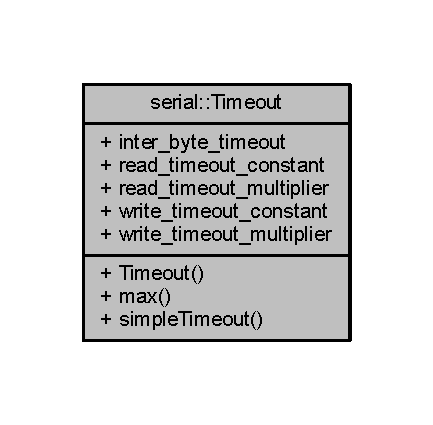
\includegraphics[width=208pt]{structserial_1_1_timeout__coll__graph}
\end{center}
\end{figure}
\subsection*{Public Member Functions}
\begin{DoxyCompactItemize}
\item 
\mbox{\hyperlink{structserial_1_1_timeout_a1a454b17f5d653b8e1b04b3ec2fead59}{Timeout}} (uint32\+\_\+t inter\+\_\+byte\+\_\+timeout\+\_\+=0, uint32\+\_\+t read\+\_\+timeout\+\_\+constant\+\_\+=0, uint32\+\_\+t read\+\_\+timeout\+\_\+multiplier\+\_\+=0, uint32\+\_\+t write\+\_\+timeout\+\_\+constant\+\_\+=0, uint32\+\_\+t write\+\_\+timeout\+\_\+multiplier\+\_\+=0)
\end{DoxyCompactItemize}
\subsection*{Static Public Member Functions}
\begin{DoxyCompactItemize}
\item 
static uint32\+\_\+t \mbox{\hyperlink{structserial_1_1_timeout_adc68e33d2f94bfa33ba1062c363b9151}{max}} ()
\item 
static \mbox{\hyperlink{structserial_1_1_timeout}{Timeout}} \mbox{\hyperlink{structserial_1_1_timeout_aa4fbd72e16f47c9aea9fb3c32ca17828}{simple\+Timeout}} (uint32\+\_\+t timeout)
\end{DoxyCompactItemize}
\subsection*{Public Attributes}
\begin{DoxyCompactItemize}
\item 
uint32\+\_\+t \mbox{\hyperlink{structserial_1_1_timeout_ada15f2a0ae478cbb62ef79d1633b2b81}{inter\+\_\+byte\+\_\+timeout}}
\item 
uint32\+\_\+t \mbox{\hyperlink{structserial_1_1_timeout_a099244649dec66b6e0548480edeb2b9f}{read\+\_\+timeout\+\_\+constant}}
\item 
uint32\+\_\+t \mbox{\hyperlink{structserial_1_1_timeout_a64412753eb2edf1621716dd9f1a4e71e}{read\+\_\+timeout\+\_\+multiplier}}
\item 
uint32\+\_\+t \mbox{\hyperlink{structserial_1_1_timeout_accf01b97f83564f4ce3d6e5f63e21006}{write\+\_\+timeout\+\_\+constant}}
\item 
uint32\+\_\+t \mbox{\hyperlink{structserial_1_1_timeout_a31ddae32907cff9c3d27fa763981317d}{write\+\_\+timeout\+\_\+multiplier}}
\end{DoxyCompactItemize}


\subsection{Detailed Description}
Structure for setting the timeout of the serial port, times are in milliseconds.

In order to disable the interbyte timeout, set it to \mbox{\hyperlink{structserial_1_1_timeout_adc68e33d2f94bfa33ba1062c363b9151}{Timeout\+::max()}}. 

\subsection{Constructor \& Destructor Documentation}
\mbox{\Hypertarget{structserial_1_1_timeout_a1a454b17f5d653b8e1b04b3ec2fead59}\label{structserial_1_1_timeout_a1a454b17f5d653b8e1b04b3ec2fead59}} 
\index{serial\+::\+Timeout@{serial\+::\+Timeout}!Timeout@{Timeout}}
\index{Timeout@{Timeout}!serial\+::\+Timeout@{serial\+::\+Timeout}}
\subsubsection{\texorpdfstring{Timeout()}{Timeout()}}
{\footnotesize\ttfamily serial\+::\+Timeout\+::\+Timeout (\begin{DoxyParamCaption}\item[{uint32\+\_\+t}]{inter\+\_\+byte\+\_\+timeout\+\_\+ = {\ttfamily 0},  }\item[{uint32\+\_\+t}]{read\+\_\+timeout\+\_\+constant\+\_\+ = {\ttfamily 0},  }\item[{uint32\+\_\+t}]{read\+\_\+timeout\+\_\+multiplier\+\_\+ = {\ttfamily 0},  }\item[{uint32\+\_\+t}]{write\+\_\+timeout\+\_\+constant\+\_\+ = {\ttfamily 0},  }\item[{uint32\+\_\+t}]{write\+\_\+timeout\+\_\+multiplier\+\_\+ = {\ttfamily 0} }\end{DoxyParamCaption})\hspace{0.3cm}{\ttfamily [inline]}, {\ttfamily [explicit]}}



\subsection{Member Function Documentation}
\mbox{\Hypertarget{structserial_1_1_timeout_adc68e33d2f94bfa33ba1062c363b9151}\label{structserial_1_1_timeout_adc68e33d2f94bfa33ba1062c363b9151}} 
\index{serial\+::\+Timeout@{serial\+::\+Timeout}!max@{max}}
\index{max@{max}!serial\+::\+Timeout@{serial\+::\+Timeout}}
\subsubsection{\texorpdfstring{max()}{max()}}
{\footnotesize\ttfamily static uint32\+\_\+t serial\+::\+Timeout\+::max (\begin{DoxyParamCaption}{ }\end{DoxyParamCaption})\hspace{0.3cm}{\ttfamily [inline]}, {\ttfamily [static]}}

\mbox{\Hypertarget{structserial_1_1_timeout_aa4fbd72e16f47c9aea9fb3c32ca17828}\label{structserial_1_1_timeout_aa4fbd72e16f47c9aea9fb3c32ca17828}} 
\index{serial\+::\+Timeout@{serial\+::\+Timeout}!simple\+Timeout@{simple\+Timeout}}
\index{simple\+Timeout@{simple\+Timeout}!serial\+::\+Timeout@{serial\+::\+Timeout}}
\subsubsection{\texorpdfstring{simple\+Timeout()}{simpleTimeout()}}
{\footnotesize\ttfamily static \mbox{\hyperlink{structserial_1_1_timeout}{Timeout}} serial\+::\+Timeout\+::simple\+Timeout (\begin{DoxyParamCaption}\item[{uint32\+\_\+t}]{timeout }\end{DoxyParamCaption})\hspace{0.3cm}{\ttfamily [inline]}, {\ttfamily [static]}}

Convenience function to generate \mbox{\hyperlink{structserial_1_1_timeout}{Timeout}} structs using a single absolute timeout.


\begin{DoxyParams}{Parameters}
{\em timeout} & A long that defines the time in milliseconds until a timeout occurs after a call to read or write is made.\\
\hline
\end{DoxyParams}
\begin{DoxyReturn}{Returns}
\mbox{\hyperlink{structserial_1_1_timeout}{Timeout}} struct that represents this simple timeout provided. 
\end{DoxyReturn}


\subsection{Member Data Documentation}
\mbox{\Hypertarget{structserial_1_1_timeout_ada15f2a0ae478cbb62ef79d1633b2b81}\label{structserial_1_1_timeout_ada15f2a0ae478cbb62ef79d1633b2b81}} 
\index{serial\+::\+Timeout@{serial\+::\+Timeout}!inter\+\_\+byte\+\_\+timeout@{inter\+\_\+byte\+\_\+timeout}}
\index{inter\+\_\+byte\+\_\+timeout@{inter\+\_\+byte\+\_\+timeout}!serial\+::\+Timeout@{serial\+::\+Timeout}}
\subsubsection{\texorpdfstring{inter\+\_\+byte\+\_\+timeout}{inter\_byte\_timeout}}
{\footnotesize\ttfamily uint32\+\_\+t serial\+::\+Timeout\+::inter\+\_\+byte\+\_\+timeout}

Number of milliseconds between bytes received to timeout on. \mbox{\Hypertarget{structserial_1_1_timeout_a099244649dec66b6e0548480edeb2b9f}\label{structserial_1_1_timeout_a099244649dec66b6e0548480edeb2b9f}} 
\index{serial\+::\+Timeout@{serial\+::\+Timeout}!read\+\_\+timeout\+\_\+constant@{read\+\_\+timeout\+\_\+constant}}
\index{read\+\_\+timeout\+\_\+constant@{read\+\_\+timeout\+\_\+constant}!serial\+::\+Timeout@{serial\+::\+Timeout}}
\subsubsection{\texorpdfstring{read\+\_\+timeout\+\_\+constant}{read\_timeout\_constant}}
{\footnotesize\ttfamily uint32\+\_\+t serial\+::\+Timeout\+::read\+\_\+timeout\+\_\+constant}

A constant number of milliseconds to wait after calling read. \mbox{\Hypertarget{structserial_1_1_timeout_a64412753eb2edf1621716dd9f1a4e71e}\label{structserial_1_1_timeout_a64412753eb2edf1621716dd9f1a4e71e}} 
\index{serial\+::\+Timeout@{serial\+::\+Timeout}!read\+\_\+timeout\+\_\+multiplier@{read\+\_\+timeout\+\_\+multiplier}}
\index{read\+\_\+timeout\+\_\+multiplier@{read\+\_\+timeout\+\_\+multiplier}!serial\+::\+Timeout@{serial\+::\+Timeout}}
\subsubsection{\texorpdfstring{read\+\_\+timeout\+\_\+multiplier}{read\_timeout\_multiplier}}
{\footnotesize\ttfamily uint32\+\_\+t serial\+::\+Timeout\+::read\+\_\+timeout\+\_\+multiplier}

A multiplier against the number of requested bytes to wait after calling read. \mbox{\Hypertarget{structserial_1_1_timeout_accf01b97f83564f4ce3d6e5f63e21006}\label{structserial_1_1_timeout_accf01b97f83564f4ce3d6e5f63e21006}} 
\index{serial\+::\+Timeout@{serial\+::\+Timeout}!write\+\_\+timeout\+\_\+constant@{write\+\_\+timeout\+\_\+constant}}
\index{write\+\_\+timeout\+\_\+constant@{write\+\_\+timeout\+\_\+constant}!serial\+::\+Timeout@{serial\+::\+Timeout}}
\subsubsection{\texorpdfstring{write\+\_\+timeout\+\_\+constant}{write\_timeout\_constant}}
{\footnotesize\ttfamily uint32\+\_\+t serial\+::\+Timeout\+::write\+\_\+timeout\+\_\+constant}

A constant number of milliseconds to wait after calling write. \mbox{\Hypertarget{structserial_1_1_timeout_a31ddae32907cff9c3d27fa763981317d}\label{structserial_1_1_timeout_a31ddae32907cff9c3d27fa763981317d}} 
\index{serial\+::\+Timeout@{serial\+::\+Timeout}!write\+\_\+timeout\+\_\+multiplier@{write\+\_\+timeout\+\_\+multiplier}}
\index{write\+\_\+timeout\+\_\+multiplier@{write\+\_\+timeout\+\_\+multiplier}!serial\+::\+Timeout@{serial\+::\+Timeout}}
\subsubsection{\texorpdfstring{write\+\_\+timeout\+\_\+multiplier}{write\_timeout\_multiplier}}
{\footnotesize\ttfamily uint32\+\_\+t serial\+::\+Timeout\+::write\+\_\+timeout\+\_\+multiplier}

A multiplier against the number of requested bytes to wait after calling write. 

The documentation for this struct was generated from the following file\+:\begin{DoxyCompactItemize}
\item 
C\+:/folders/d/scripts/cpp/\+O\+P\+T3101\+S\+D\+K/\+O\+P\+T3101\+S\+D\+K/\+O\+P\+T3101\+S\+D\+K/serial\+Lib/\mbox{\hyperlink{serial_8h}{serial.\+h}}\end{DoxyCompactItemize}

\chapter{File Documentation}
\hypertarget{mainpage_8markdown}{}\section{C\+:/folders/d/scripts/cpp/\+O\+P\+T3101\+S\+D\+K/\+O\+P\+T3101\+S\+D\+K/doc/mainpage.markdown File Reference}
\label{mainpage_8markdown}\index{C\+:/folders/d/scripts/cpp/\+O\+P\+T3101\+S\+D\+K/\+O\+P\+T3101\+S\+D\+K/doc/mainpage.\+markdown@{C\+:/folders/d/scripts/cpp/\+O\+P\+T3101\+S\+D\+K/\+O\+P\+T3101\+S\+D\+K/doc/mainpage.\+markdown}}

\hypertarget{environment_control_8cpp}{}\section{C\+:/folders/d/scripts/cpp/\+O\+P\+T3101\+S\+D\+K/\+O\+P\+T3101\+S\+D\+K/\+O\+P\+T3101\+S\+D\+K/environment\+Control.cpp File Reference}
\label{environment_control_8cpp}\index{C\+:/folders/d/scripts/cpp/\+O\+P\+T3101\+S\+D\+K/\+O\+P\+T3101\+S\+D\+K/\+O\+P\+T3101\+S\+D\+K/environment\+Control.\+cpp@{C\+:/folders/d/scripts/cpp/\+O\+P\+T3101\+S\+D\+K/\+O\+P\+T3101\+S\+D\+K/\+O\+P\+T3101\+S\+D\+K/environment\+Control.\+cpp}}
{\ttfamily \#include \char`\"{}environment\+Control.\+h\char`\"{}}\newline
Include dependency graph for environment\+Control.\+cpp\+:\nopagebreak
\begin{figure}[H]
\begin{center}
\leavevmode
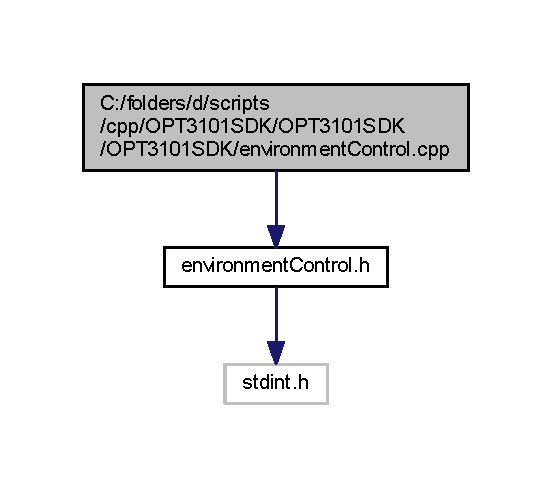
\includegraphics[width=265pt]{environment_control_8cpp__incl}
\end{center}
\end{figure}
\subsection*{Variables}
\begin{DoxyCompactItemize}
\item 
\mbox{\hyperlink{classenvironmental_controller}{environmental\+Controller}} \mbox{\hyperlink{environment_control_8cpp_abf2c91dbdc70c87e1f27292a948c77ab}{env\+Controller}}
\begin{DoxyCompactList}\small\item\em \mbox{\hyperlink{classenvironmental_controller}{environmental\+Controller}} declaration This global variable declaration with name env\+Controller of \mbox{\hyperlink{classenvironmental_controller}{environmental\+Controller}} is used by class for various environmental setup during calibration steps \end{DoxyCompactList}\end{DoxyCompactItemize}


\subsection{Detailed Description}
\begin{DoxyAuthor}{Author}
Karthik Rajagopal \href{mailto:krthik@ti.com}{\tt krthik@ti.\+com} 
\end{DoxyAuthor}
\begin{DoxyVersion}{Version}
0.\+8
\end{DoxyVersion}
\hypertarget{register_8h_COPYRIGHT}{}\subsection{C\+O\+P\+Y\+R\+I\+G\+HT}\label{register_8h_COPYRIGHT}
T\+E\+X\+AS I\+N\+S\+T\+R\+U\+M\+E\+N\+TS T\+E\+XT F\+I\+LE L\+I\+C\+E\+N\+SE Copyright (c) 2018 Texas Instruments Incorporated All rights reserved not granted herein. Limited License. Texas Instruments Incorporated grants a world-\/wide, royalty-\/free, non-\/exclusive license under copyrights and patents it now or hereafter owns or controls to make, have made, use, import, offer to sell and sell (\char`\"{}\+Utilize\char`\"{}) this software subject to the terms herein. With respect to the foregoing patent license, such license is granted solely to the extent that any such patent is necessary to Utilize the software alone. The patent license shall not apply to any combinations which include this software, other than combinations with devices manufactured by or for TI (“\+TI Devices”). No hardware patent is licensed hereunder. Redistributions must preserve existing copyright notices and reproduce this license (including the above copyright notice and the disclaimer and (if applicable) source code license limitations below) in the documentation and/or other materials provided with the distribution Redistribution and use in binary form, without modification, are permitted provided that the following conditions are met\+:
\begin{DoxyItemize}
\item No reverse engineering, decompilation, or disassembly of this software is permitted with respect to any software provided in binary form.
\item any redistribution and use are licensed by TI for use only with TI Devices.
\item Nothing shall obligate TI to provide you with source code for the software licensed and provided to you in object code. If software source code is provided to you, modification and redistribution of the source code are permitted provided that the following conditions are met\+:
\item any redistribution and use of the source code, including any resulting derivative works, are licensed by TI for use only with TI Devices.
\item any redistribution and use of any object code compiled from the source code and any resulting derivative works, are licensed by TI for use only with TI Devices. Neither the name of Texas Instruments Incorporated nor the names of its suppliers may be used to endorse or promote products derived from this software without specific prior written permission. D\+I\+S\+C\+L\+A\+I\+M\+ER. T\+H\+IS S\+O\+F\+T\+W\+A\+RE IS P\+R\+O\+V\+I\+D\+ED BY TI A\+ND T\+I’S L\+I\+C\+E\+N\+S\+O\+RS \char`\"{}\+A\+S I\+S\char`\"{} A\+ND A\+NY E\+X\+P\+R\+E\+SS OR I\+M\+P\+L\+I\+ED W\+A\+R\+R\+A\+N\+T\+I\+ES, I\+N\+C\+L\+U\+D\+I\+NG, B\+UT N\+OT L\+I\+M\+I\+T\+ED TO, T\+HE I\+M\+P\+L\+I\+ED W\+A\+R\+R\+A\+N\+T\+I\+ES OF M\+E\+R\+C\+H\+A\+N\+T\+A\+B\+I\+L\+I\+TY A\+ND F\+I\+T\+N\+E\+SS F\+OR A P\+A\+R\+T\+I\+C\+U\+L\+AR P\+U\+R\+P\+O\+SE A\+RE D\+I\+S\+C\+L\+A\+I\+M\+ED. IN NO E\+V\+E\+NT S\+H\+A\+LL TI A\+ND T\+I’S L\+I\+C\+E\+N\+S\+O\+RS BE L\+I\+A\+B\+LE F\+OR A\+NY D\+I\+R\+E\+CT, I\+N\+D\+I\+R\+E\+CT, I\+N\+C\+I\+D\+E\+N\+T\+AL, S\+P\+E\+C\+I\+AL, E\+X\+E\+M\+P\+L\+A\+RY, OR C\+O\+N\+S\+E\+Q\+U\+E\+N\+T\+I\+AL D\+A\+M\+A\+G\+ES (I\+N\+C\+L\+U\+D\+I\+NG, B\+UT N\+OT L\+I\+M\+I\+T\+ED TO, P\+R\+O\+C\+U\+R\+E\+M\+E\+NT OF S\+U\+B\+S\+T\+I\+T\+U\+TE G\+O\+O\+DS OR S\+E\+R\+V\+I\+C\+ES; L\+O\+SS OF U\+SE, D\+A\+TA, OR P\+R\+O\+F\+I\+TS; OR B\+U\+S\+I\+N\+E\+SS I\+N\+T\+E\+R\+R\+U\+P\+T\+I\+ON) H\+O\+W\+E\+V\+ER C\+A\+U\+S\+ED A\+ND ON A\+NY T\+H\+E\+O\+RY OF L\+I\+A\+B\+I\+L\+I\+TY, W\+H\+E\+T\+H\+ER IN C\+O\+N\+T\+R\+A\+CT, S\+T\+R\+I\+CT L\+I\+A\+B\+I\+L\+I\+TY, OR T\+O\+RT (I\+N\+C\+L\+U\+D\+I\+NG N\+E\+G\+L\+I\+G\+E\+N\+CE OR O\+T\+H\+E\+R\+W\+I\+SE) A\+R\+I\+S\+I\+NG IN A\+NY W\+AY O\+UT OF T\+HE U\+SE OF T\+H\+IS S\+O\+F\+T\+W\+A\+RE, E\+V\+EN IF A\+D\+V\+I\+S\+ED OF T\+HE P\+O\+S\+S\+I\+B\+I\+L\+I\+TY OF S\+U\+CH D\+A\+M\+A\+GE.
\end{DoxyItemize}\hypertarget{register_8h_DESCRIPTION}{}\subsection{D\+E\+S\+C\+R\+I\+P\+T\+I\+ON}\label{register_8h_DESCRIPTION}
The file contains class \mbox{\hyperlink{classenvironmental_controller}{environmental\+Controller}} methods and declaration 

\subsection{Variable Documentation}
\mbox{\Hypertarget{environment_control_8cpp_abf2c91dbdc70c87e1f27292a948c77ab}\label{environment_control_8cpp_abf2c91dbdc70c87e1f27292a948c77ab}} 
\index{environment\+Control.\+cpp@{environment\+Control.\+cpp}!env\+Controller@{env\+Controller}}
\index{env\+Controller@{env\+Controller}!environment\+Control.\+cpp@{environment\+Control.\+cpp}}
\subsubsection{\texorpdfstring{env\+Controller}{envController}}
{\footnotesize\ttfamily \mbox{\hyperlink{classenvironmental_controller}{environmental\+Controller}} env\+Controller}



\mbox{\hyperlink{classenvironmental_controller}{environmental\+Controller}} declaration This global variable declaration with name env\+Controller of \mbox{\hyperlink{classenvironmental_controller}{environmental\+Controller}} is used by class for various environmental setup during calibration steps 

\mbox{\hyperlink{classenvironmental_controller}{environmental\+Controller}} class instance declaration This global variable declaration to be available across files which controls the environmental parameters. The instance is of class \mbox{\hyperlink{classenvironmental_controller}{environmental\+Controller}} 
\hypertarget{environment_control_8h}{}\section{C\+:/folders/d/scripts/cpp/\+O\+P\+T3101\+S\+D\+K/\+O\+P\+T3101\+S\+D\+K/\+O\+P\+T3101\+S\+D\+K/environment\+Control.h File Reference}
\label{environment_control_8h}\index{C\+:/folders/d/scripts/cpp/\+O\+P\+T3101\+S\+D\+K/\+O\+P\+T3101\+S\+D\+K/\+O\+P\+T3101\+S\+D\+K/environment\+Control.\+h@{C\+:/folders/d/scripts/cpp/\+O\+P\+T3101\+S\+D\+K/\+O\+P\+T3101\+S\+D\+K/\+O\+P\+T3101\+S\+D\+K/environment\+Control.\+h}}
{\ttfamily \#include $<$stdint.\+h$>$}\newline
Include dependency graph for environment\+Control.\+h\+:\nopagebreak
\begin{figure}[H]
\begin{center}
\leavevmode
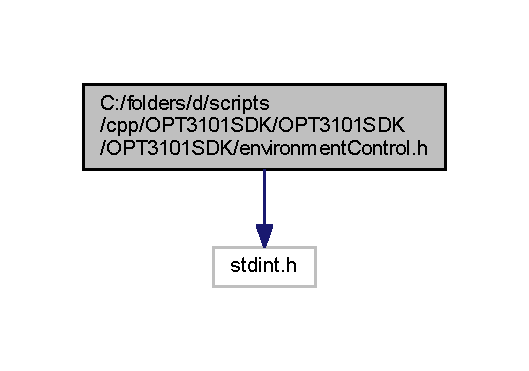
\includegraphics[width=254pt]{environment_control_8h__incl}
\end{center}
\end{figure}
This graph shows which files directly or indirectly include this file\+:\nopagebreak
\begin{figure}[H]
\begin{center}
\leavevmode
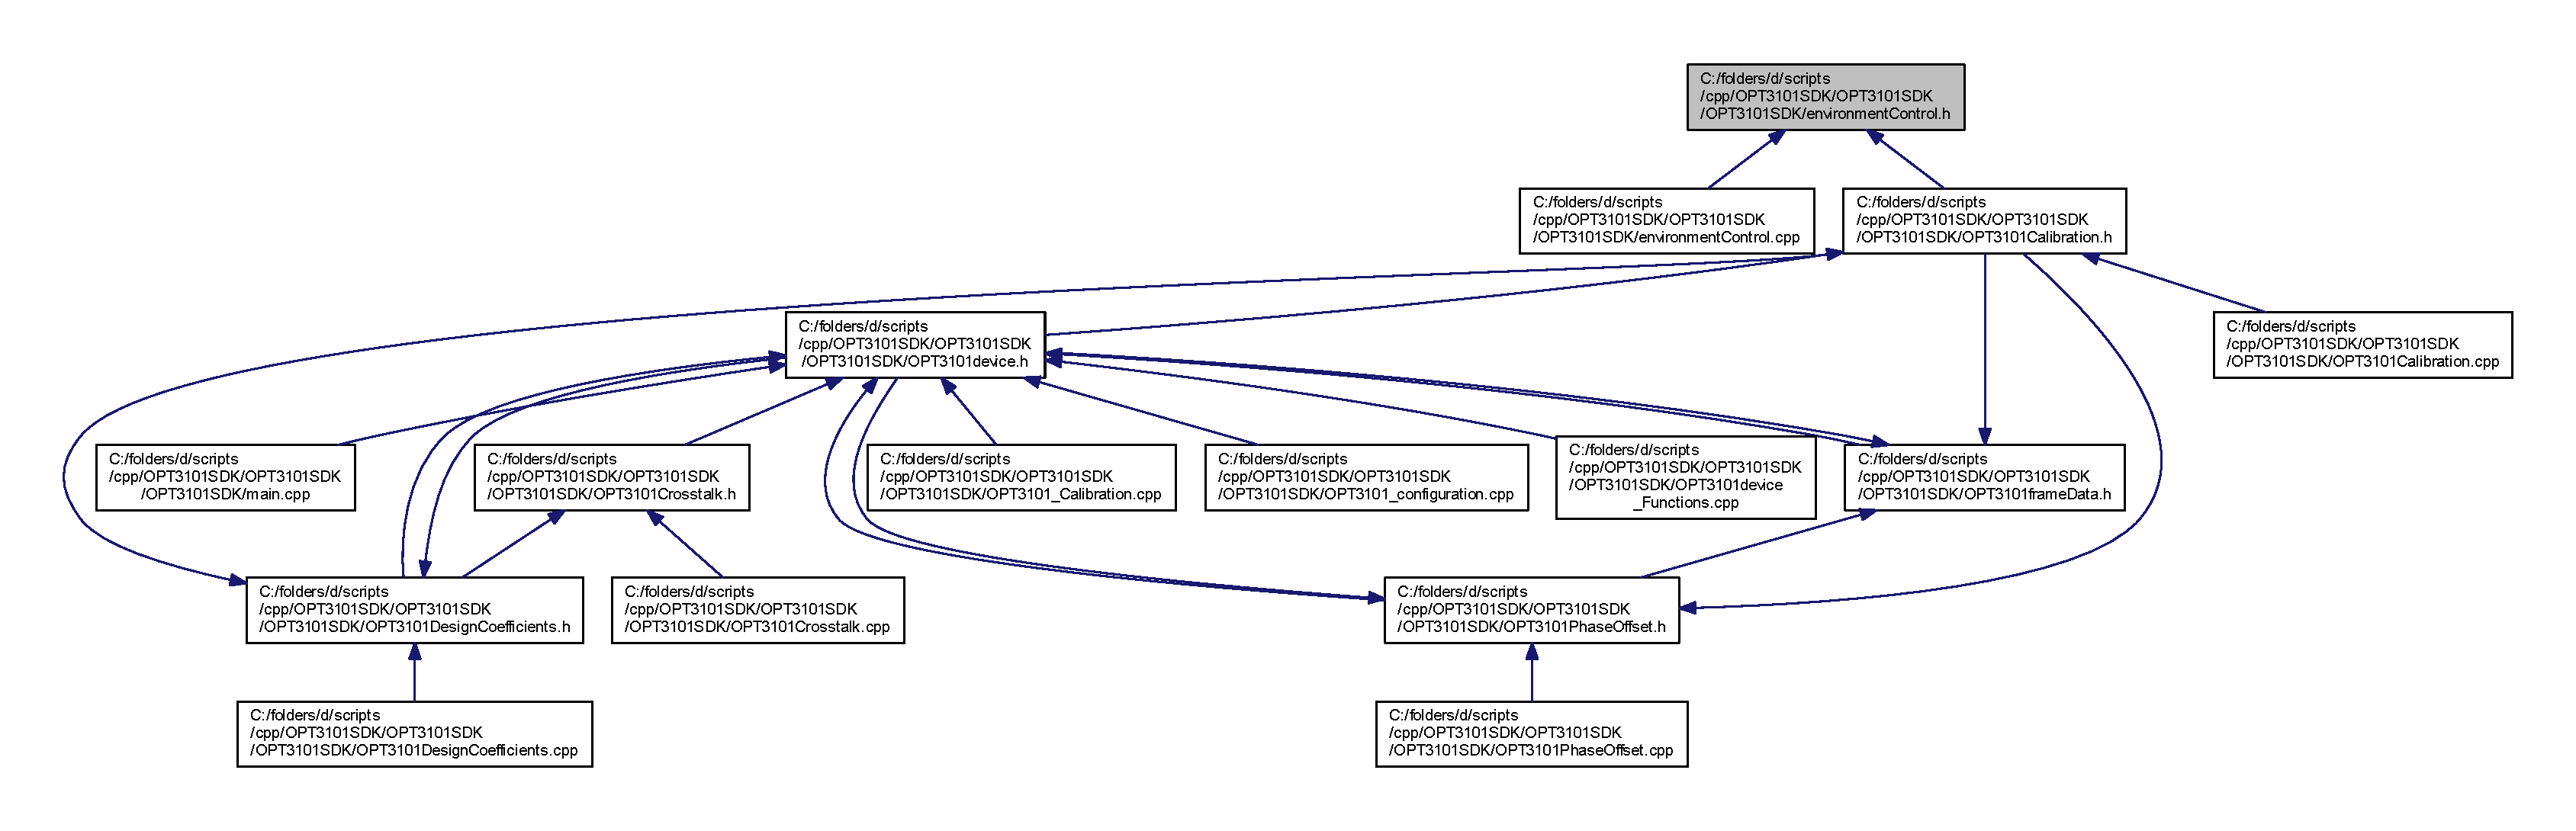
\includegraphics[width=350pt]{environment_control_8h__dep__incl}
\end{center}
\end{figure}
\subsection*{Classes}
\begin{DoxyCompactItemize}
\item 
class \mbox{\hyperlink{classenvironmental_controller}{environmental\+Controller}}
\begin{DoxyCompactList}\small\item\em Generic implementation for environment controller. \end{DoxyCompactList}\end{DoxyCompactItemize}


\subsection{Detailed Description}
\begin{DoxyAuthor}{Author}
Karthik Rajagopal \href{mailto:krthik@ti.com}{\tt krthik@ti.\+com} 
\end{DoxyAuthor}
\begin{DoxyVersion}{Version}
0.\+8
\end{DoxyVersion}
\hypertarget{register_8h_COPYRIGHT}{}\subsection{C\+O\+P\+Y\+R\+I\+G\+HT}\label{register_8h_COPYRIGHT}
T\+E\+X\+AS I\+N\+S\+T\+R\+U\+M\+E\+N\+TS T\+E\+XT F\+I\+LE L\+I\+C\+E\+N\+SE Copyright (c) 2018 Texas Instruments Incorporated All rights reserved not granted herein. Limited License. Texas Instruments Incorporated grants a world-\/wide, royalty-\/free, non-\/exclusive license under copyrights and patents it now or hereafter owns or controls to make, have made, use, import, offer to sell and sell (\char`\"{}\+Utilize\char`\"{}) this software subject to the terms herein. With respect to the foregoing patent license, such license is granted solely to the extent that any such patent is necessary to Utilize the software alone. The patent license shall not apply to any combinations which include this software, other than combinations with devices manufactured by or for TI (“\+TI Devices”). No hardware patent is licensed hereunder. Redistributions must preserve existing copyright notices and reproduce this license (including the above copyright notice and the disclaimer and (if applicable) source code license limitations below) in the documentation and/or other materials provided with the distribution Redistribution and use in binary form, without modification, are permitted provided that the following conditions are met\+:
\begin{DoxyItemize}
\item No reverse engineering, decompilation, or disassembly of this software is permitted with respect to any software provided in binary form.
\item any redistribution and use are licensed by TI for use only with TI Devices.
\item Nothing shall obligate TI to provide you with source code for the software licensed and provided to you in object code. If software source code is provided to you, modification and redistribution of the source code are permitted provided that the following conditions are met\+:
\item any redistribution and use of the source code, including any resulting derivative works, are licensed by TI for use only with TI Devices.
\item any redistribution and use of any object code compiled from the source code and any resulting derivative works, are licensed by TI for use only with TI Devices. Neither the name of Texas Instruments Incorporated nor the names of its suppliers may be used to endorse or promote products derived from this software without specific prior written permission. D\+I\+S\+C\+L\+A\+I\+M\+ER. T\+H\+IS S\+O\+F\+T\+W\+A\+RE IS P\+R\+O\+V\+I\+D\+ED BY TI A\+ND T\+I’S L\+I\+C\+E\+N\+S\+O\+RS \char`\"{}\+A\+S I\+S\char`\"{} A\+ND A\+NY E\+X\+P\+R\+E\+SS OR I\+M\+P\+L\+I\+ED W\+A\+R\+R\+A\+N\+T\+I\+ES, I\+N\+C\+L\+U\+D\+I\+NG, B\+UT N\+OT L\+I\+M\+I\+T\+ED TO, T\+HE I\+M\+P\+L\+I\+ED W\+A\+R\+R\+A\+N\+T\+I\+ES OF M\+E\+R\+C\+H\+A\+N\+T\+A\+B\+I\+L\+I\+TY A\+ND F\+I\+T\+N\+E\+SS F\+OR A P\+A\+R\+T\+I\+C\+U\+L\+AR P\+U\+R\+P\+O\+SE A\+RE D\+I\+S\+C\+L\+A\+I\+M\+ED. IN NO E\+V\+E\+NT S\+H\+A\+LL TI A\+ND T\+I’S L\+I\+C\+E\+N\+S\+O\+RS BE L\+I\+A\+B\+LE F\+OR A\+NY D\+I\+R\+E\+CT, I\+N\+D\+I\+R\+E\+CT, I\+N\+C\+I\+D\+E\+N\+T\+AL, S\+P\+E\+C\+I\+AL, E\+X\+E\+M\+P\+L\+A\+RY, OR C\+O\+N\+S\+E\+Q\+U\+E\+N\+T\+I\+AL D\+A\+M\+A\+G\+ES (I\+N\+C\+L\+U\+D\+I\+NG, B\+UT N\+OT L\+I\+M\+I\+T\+ED TO, P\+R\+O\+C\+U\+R\+E\+M\+E\+NT OF S\+U\+B\+S\+T\+I\+T\+U\+TE G\+O\+O\+DS OR S\+E\+R\+V\+I\+C\+ES; L\+O\+SS OF U\+SE, D\+A\+TA, OR P\+R\+O\+F\+I\+TS; OR B\+U\+S\+I\+N\+E\+SS I\+N\+T\+E\+R\+R\+U\+P\+T\+I\+ON) H\+O\+W\+E\+V\+ER C\+A\+U\+S\+ED A\+ND ON A\+NY T\+H\+E\+O\+RY OF L\+I\+A\+B\+I\+L\+I\+TY, W\+H\+E\+T\+H\+ER IN C\+O\+N\+T\+R\+A\+CT, S\+T\+R\+I\+CT L\+I\+A\+B\+I\+L\+I\+TY, OR T\+O\+RT (I\+N\+C\+L\+U\+D\+I\+NG N\+E\+G\+L\+I\+G\+E\+N\+CE OR O\+T\+H\+E\+R\+W\+I\+SE) A\+R\+I\+S\+I\+NG IN A\+NY W\+AY O\+UT OF T\+HE U\+SE OF T\+H\+IS S\+O\+F\+T\+W\+A\+RE, E\+V\+EN IF A\+D\+V\+I\+S\+ED OF T\+HE P\+O\+S\+S\+I\+B\+I\+L\+I\+TY OF S\+U\+CH D\+A\+M\+A\+GE.
\end{DoxyItemize}\hypertarget{register_8h_DESCRIPTION}{}\subsection{D\+E\+S\+C\+R\+I\+P\+T\+I\+ON}\label{register_8h_DESCRIPTION}
The file contains class descriptions and methods for environment control 
\hypertarget{host_controller_8cpp}{}\section{C\+:/folders/d/scripts/cpp/\+O\+P\+T3101\+S\+D\+K/\+O\+P\+T3101\+S\+D\+K/\+O\+P\+T3101\+S\+D\+K/host\+Controller.cpp File Reference}
\label{host_controller_8cpp}\index{C\+:/folders/d/scripts/cpp/\+O\+P\+T3101\+S\+D\+K/\+O\+P\+T3101\+S\+D\+K/\+O\+P\+T3101\+S\+D\+K/host\+Controller.\+cpp@{C\+:/folders/d/scripts/cpp/\+O\+P\+T3101\+S\+D\+K/\+O\+P\+T3101\+S\+D\+K/\+O\+P\+T3101\+S\+D\+K/host\+Controller.\+cpp}}
{\ttfamily \#include \char`\"{}host\+Controller.\+h\char`\"{}}\newline
Include dependency graph for host\+Controller.\+cpp\+:\nopagebreak
\begin{figure}[H]
\begin{center}
\leavevmode
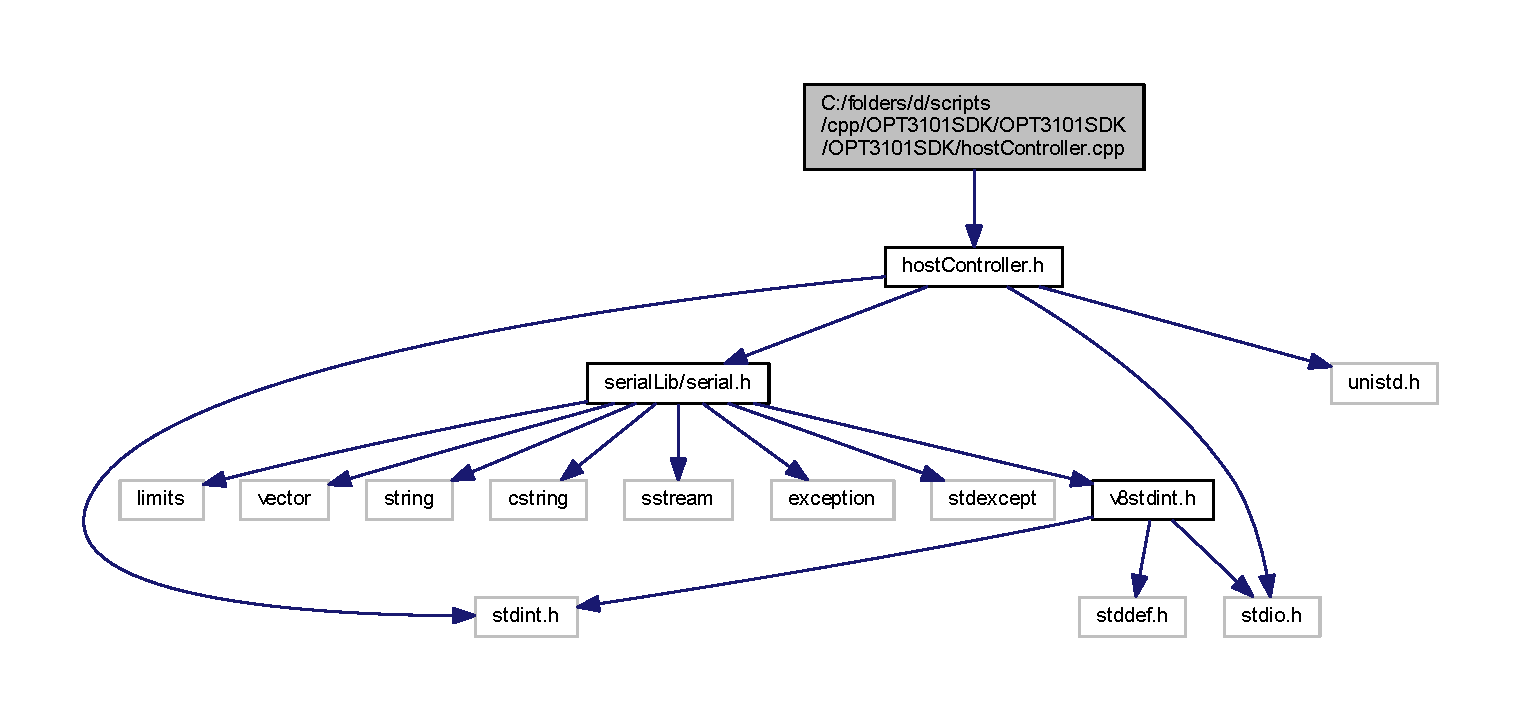
\includegraphics[width=350pt]{host_controller_8cpp__incl}
\end{center}
\end{figure}
\subsection*{Variables}
\begin{DoxyCompactItemize}
\item 
\mbox{\hyperlink{classserial_1_1_serial}{serial\+::\+Serial}} \mbox{\hyperlink{host_controller_8cpp_ae42ea63290ca9d783d7de13cd64b6b88}{O\+P\+T3101command\+Port}} (\char`\"{}C\+O\+M43\char`\"{}, 9600, serial\+::\+Timeout\+::simple\+Timeout(1000))
\begin{DoxyCompactList}\small\item\em Serial Command Port declaration This global variable declaration with name O\+P\+T3101command\+Port of class \mbox{\hyperlink{classserial_1_1_serial}{serial\+::\+Serial}} is used by class like \mbox{\hyperlink{class_o_p_t3101_1_1device_register}{O\+P\+T3101\+::device\+Register}} for I2C read and writes. \end{DoxyCompactList}\item 
const char \mbox{\hyperlink{host_controller_8cpp_a84ce75d62690cdf4061bfa917ce90bc8}{file\+Path}} \mbox{[}$\,$\mbox{]} = \{ \char`\"{}C\+:/temp/\char`\"{} \}
\begin{DoxyCompactList}\small\item\em file\+Path This global variable to declare a path to all calibration files storage \end{DoxyCompactList}\item 
\mbox{\hyperlink{classhost_controller}{host\+Controller}} \mbox{\hyperlink{host_controller_8cpp_a47f8cbf152e48aa4fdb624be57a9a856}{host}}
\begin{DoxyCompactList}\small\item\em \mbox{\hyperlink{classhost_controller}{host\+Controller}} declaration This global variable declaration with name host of class \mbox{\hyperlink{classhost_controller}{host\+Controller}} is used by various different classes like \mbox{\hyperlink{class_o_p_t3101_1_1device_register}{O\+P\+T3101\+::device\+Register}} , \mbox{\hyperlink{class_o_p_t3101_1_1registers}{O\+P\+T3101\+::registers}} and \mbox{\hyperlink{class_o_p_t3101_1_1device}{O\+P\+T3101\+::device}} to specify specific instructions to the host like wait, sleep, I2C reads and writes \end{DoxyCompactList}\end{DoxyCompactItemize}


\subsection{Detailed Description}
\begin{DoxyAuthor}{Author}
Karthik Rajagopal \href{mailto:krthik@ti.com}{\tt krthik@ti.\+com} 
\end{DoxyAuthor}
\begin{DoxyVersion}{Version}
0.\+8
\end{DoxyVersion}
\hypertarget{register_8h_COPYRIGHT}{}\subsection{C\+O\+P\+Y\+R\+I\+G\+HT}\label{register_8h_COPYRIGHT}
T\+E\+X\+AS I\+N\+S\+T\+R\+U\+M\+E\+N\+TS T\+E\+XT F\+I\+LE L\+I\+C\+E\+N\+SE Copyright (c) 2018 Texas Instruments Incorporated All rights reserved not granted herein. Limited License. Texas Instruments Incorporated grants a world-\/wide, royalty-\/free, non-\/exclusive license under copyrights and patents it now or hereafter owns or controls to make, have made, use, import, offer to sell and sell (\char`\"{}\+Utilize\char`\"{}) this software subject to the terms herein. With respect to the foregoing patent license, such license is granted solely to the extent that any such patent is necessary to Utilize the software alone. The patent license shall not apply to any combinations which include this software, other than combinations with devices manufactured by or for TI (�\+TI Devices�). No hardware patent is licensed hereunder. Redistributions must preserve existing copyright notices and reproduce this license (including the above copyright notice and the disclaimer and (if applicable) source code license limitations below) in the documentation and/or other materials provided with the distribution Redistribution and use in binary form, without modification, are permitted provided that the following conditions are met\+:
\begin{DoxyItemize}
\item No reverse engineering, decompilation, or disassembly of this software is permitted with respect to any software provided in binary form.
\item any redistribution and use are licensed by TI for use only with TI Devices.
\item Nothing shall obligate TI to provide you with source code for the software licensed and provided to you in object code. If software source code is provided to you, modification and redistribution of the source code are permitted provided that the following conditions are met\+:
\item any redistribution and use of the source code, including any resulting derivative works, are licensed by TI for use only with TI Devices.
\item any redistribution and use of any object code compiled from the source code and any resulting derivative works, are licensed by TI for use only with TI Devices. Neither the name of Texas Instruments Incorporated nor the names of its suppliers may be used to endorse or promote products derived from this software without specific prior written permission. D\+I\+S\+C\+L\+A\+I\+M\+ER. T\+H\+IS S\+O\+F\+T\+W\+A\+RE IS P\+R\+O\+V\+I\+D\+ED BY TI A\+ND T\+I�S L\+I\+C\+E\+N\+S\+O\+RS \char`\"{}\+A\+S I\+S\char`\"{} A\+ND A\+NY E\+X\+P\+R\+E\+SS OR I\+M\+P\+L\+I\+ED W\+A\+R\+R\+A\+N\+T\+I\+ES, I\+N\+C\+L\+U\+D\+I\+NG, B\+UT N\+OT L\+I\+M\+I\+T\+ED TO, T\+HE I\+M\+P\+L\+I\+ED W\+A\+R\+R\+A\+N\+T\+I\+ES OF M\+E\+R\+C\+H\+A\+N\+T\+A\+B\+I\+L\+I\+TY A\+ND F\+I\+T\+N\+E\+SS F\+OR A P\+A\+R\+T\+I\+C\+U\+L\+AR P\+U\+R\+P\+O\+SE A\+RE D\+I\+S\+C\+L\+A\+I\+M\+ED. IN NO E\+V\+E\+NT S\+H\+A\+LL TI A\+ND T\+I�S L\+I\+C\+E\+N\+S\+O\+RS BE L\+I\+A\+B\+LE F\+OR A\+NY D\+I\+R\+E\+CT, I\+N\+D\+I\+R\+E\+CT, I\+N\+C\+I\+D\+E\+N\+T\+AL, S\+P\+E\+C\+I\+AL, E\+X\+E\+M\+P\+L\+A\+RY, OR C\+O\+N\+S\+E\+Q\+U\+E\+N\+T\+I\+AL D\+A\+M\+A\+G\+ES (I\+N\+C\+L\+U\+D\+I\+NG, B\+UT N\+OT L\+I\+M\+I\+T\+ED TO, P\+R\+O\+C\+U\+R\+E\+M\+E\+NT OF S\+U\+B\+S\+T\+I\+T\+U\+TE G\+O\+O\+DS OR S\+E\+R\+V\+I\+C\+ES; L\+O\+SS OF U\+SE, D\+A\+TA, OR P\+R\+O\+F\+I\+TS; OR B\+U\+S\+I\+N\+E\+SS I\+N\+T\+E\+R\+R\+U\+P\+T\+I\+ON) H\+O\+W\+E\+V\+ER C\+A\+U\+S\+ED A\+ND ON A\+NY T\+H\+E\+O\+RY OF L\+I\+A\+B\+I\+L\+I\+TY, W\+H\+E\+T\+H\+ER IN C\+O\+N\+T\+R\+A\+CT, S\+T\+R\+I\+CT L\+I\+A\+B\+I\+L\+I\+TY, OR T\+O\+RT (I\+N\+C\+L\+U\+D\+I\+NG N\+E\+G\+L\+I\+G\+E\+N\+CE OR O\+T\+H\+E\+R\+W\+I\+SE) A\+R\+I\+S\+I\+NG IN A\+NY W\+AY O\+UT OF T\+HE U\+SE OF T\+H\+IS S\+O\+F\+T\+W\+A\+RE, E\+V\+EN IF A\+D\+V\+I\+S\+ED OF T\+HE P\+O\+S\+S\+I\+B\+I\+L\+I\+TY OF S\+U\+CH D\+A\+M\+A\+GE.
\end{DoxyItemize}\hypertarget{register_8h_DESCRIPTION}{}\subsection{D\+E\+S\+C\+R\+I\+P\+T\+I\+ON}\label{register_8h_DESCRIPTION}
This file contains the \mbox{\hyperlink{classhost_controller}{host\+Controller}} class methods 

\subsection{Variable Documentation}
\mbox{\Hypertarget{host_controller_8cpp_a84ce75d62690cdf4061bfa917ce90bc8}\label{host_controller_8cpp_a84ce75d62690cdf4061bfa917ce90bc8}} 
\index{host\+Controller.\+cpp@{host\+Controller.\+cpp}!file\+Path@{file\+Path}}
\index{file\+Path@{file\+Path}!host\+Controller.\+cpp@{host\+Controller.\+cpp}}
\subsubsection{\texorpdfstring{file\+Path}{filePath}}
{\footnotesize\ttfamily const char file\+Path\mbox{[}$\,$\mbox{]} = \{ \char`\"{}C\+:/temp/\char`\"{} \}}



file\+Path This global variable to declare a path to all calibration files storage 

\mbox{\Hypertarget{host_controller_8cpp_a47f8cbf152e48aa4fdb624be57a9a856}\label{host_controller_8cpp_a47f8cbf152e48aa4fdb624be57a9a856}} 
\index{host\+Controller.\+cpp@{host\+Controller.\+cpp}!host@{host}}
\index{host@{host}!host\+Controller.\+cpp@{host\+Controller.\+cpp}}
\subsubsection{\texorpdfstring{host}{host}}
{\footnotesize\ttfamily \mbox{\hyperlink{classhost_controller}{host\+Controller}} host}



\mbox{\hyperlink{classhost_controller}{host\+Controller}} declaration This global variable declaration with name host of class \mbox{\hyperlink{classhost_controller}{host\+Controller}} is used by various different classes like \mbox{\hyperlink{class_o_p_t3101_1_1device_register}{O\+P\+T3101\+::device\+Register}} , \mbox{\hyperlink{class_o_p_t3101_1_1registers}{O\+P\+T3101\+::registers}} and \mbox{\hyperlink{class_o_p_t3101_1_1device}{O\+P\+T3101\+::device}} to specify specific instructions to the host like wait, sleep, I2C reads and writes 

\mbox{\Hypertarget{host_controller_8cpp_ae42ea63290ca9d783d7de13cd64b6b88}\label{host_controller_8cpp_ae42ea63290ca9d783d7de13cd64b6b88}} 
\index{host\+Controller.\+cpp@{host\+Controller.\+cpp}!O\+P\+T3101command\+Port@{O\+P\+T3101command\+Port}}
\index{O\+P\+T3101command\+Port@{O\+P\+T3101command\+Port}!host\+Controller.\+cpp@{host\+Controller.\+cpp}}
\subsubsection{\texorpdfstring{O\+P\+T3101command\+Port}{OPT3101commandPort}}
{\footnotesize\ttfamily \mbox{\hyperlink{classserial_1_1_serial}{serial\+::\+Serial}} O\+P\+T3101command\+Port(\char`\"{}C\+O\+M43\char`\"{}, 9600, serial\+::\+Timeout\+::simple\+Timeout(1000))}



Serial Command Port declaration This global variable declaration with name O\+P\+T3101command\+Port of class \mbox{\hyperlink{classserial_1_1_serial}{serial\+::\+Serial}} is used by class like \mbox{\hyperlink{class_o_p_t3101_1_1device_register}{O\+P\+T3101\+::device\+Register}} for I2C read and writes. 


\hypertarget{host_controller_8h}{}\section{C\+:/folders/d/scripts/cpp/\+O\+P\+T3101\+S\+D\+K/\+O\+P\+T3101\+S\+D\+K/\+O\+P\+T3101\+S\+D\+K/host\+Controller.h File Reference}
\label{host_controller_8h}\index{C\+:/folders/d/scripts/cpp/\+O\+P\+T3101\+S\+D\+K/\+O\+P\+T3101\+S\+D\+K/\+O\+P\+T3101\+S\+D\+K/host\+Controller.\+h@{C\+:/folders/d/scripts/cpp/\+O\+P\+T3101\+S\+D\+K/\+O\+P\+T3101\+S\+D\+K/\+O\+P\+T3101\+S\+D\+K/host\+Controller.\+h}}
{\ttfamily \#include $<$stdint.\+h$>$}\newline
{\ttfamily \#include \char`\"{}serial\+Lib/serial.\+h\char`\"{}}\newline
{\ttfamily \#include $<$unistd.\+h$>$}\newline
{\ttfamily \#include $<$stdio.\+h$>$}\newline
Include dependency graph for host\+Controller.\+h\+:\nopagebreak
\begin{figure}[H]
\begin{center}
\leavevmode
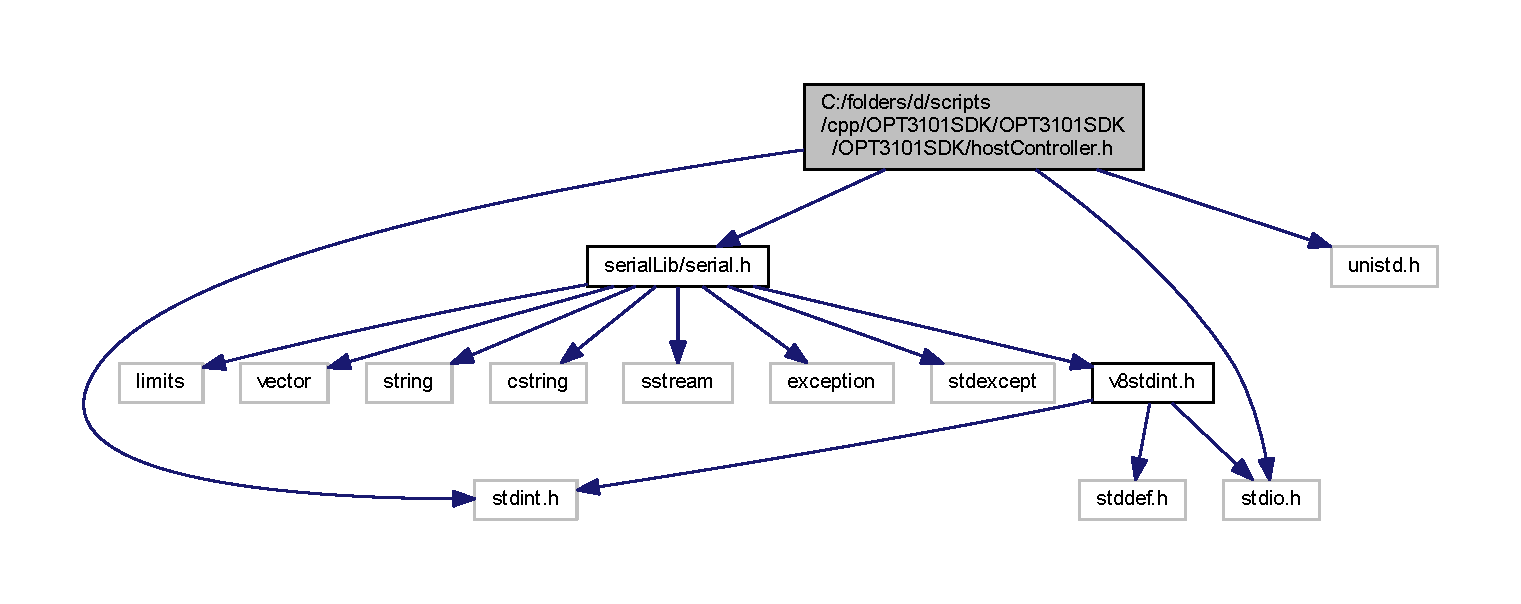
\includegraphics[width=350pt]{host_controller_8h__incl}
\end{center}
\end{figure}
This graph shows which files directly or indirectly include this file\+:\nopagebreak
\begin{figure}[H]
\begin{center}
\leavevmode
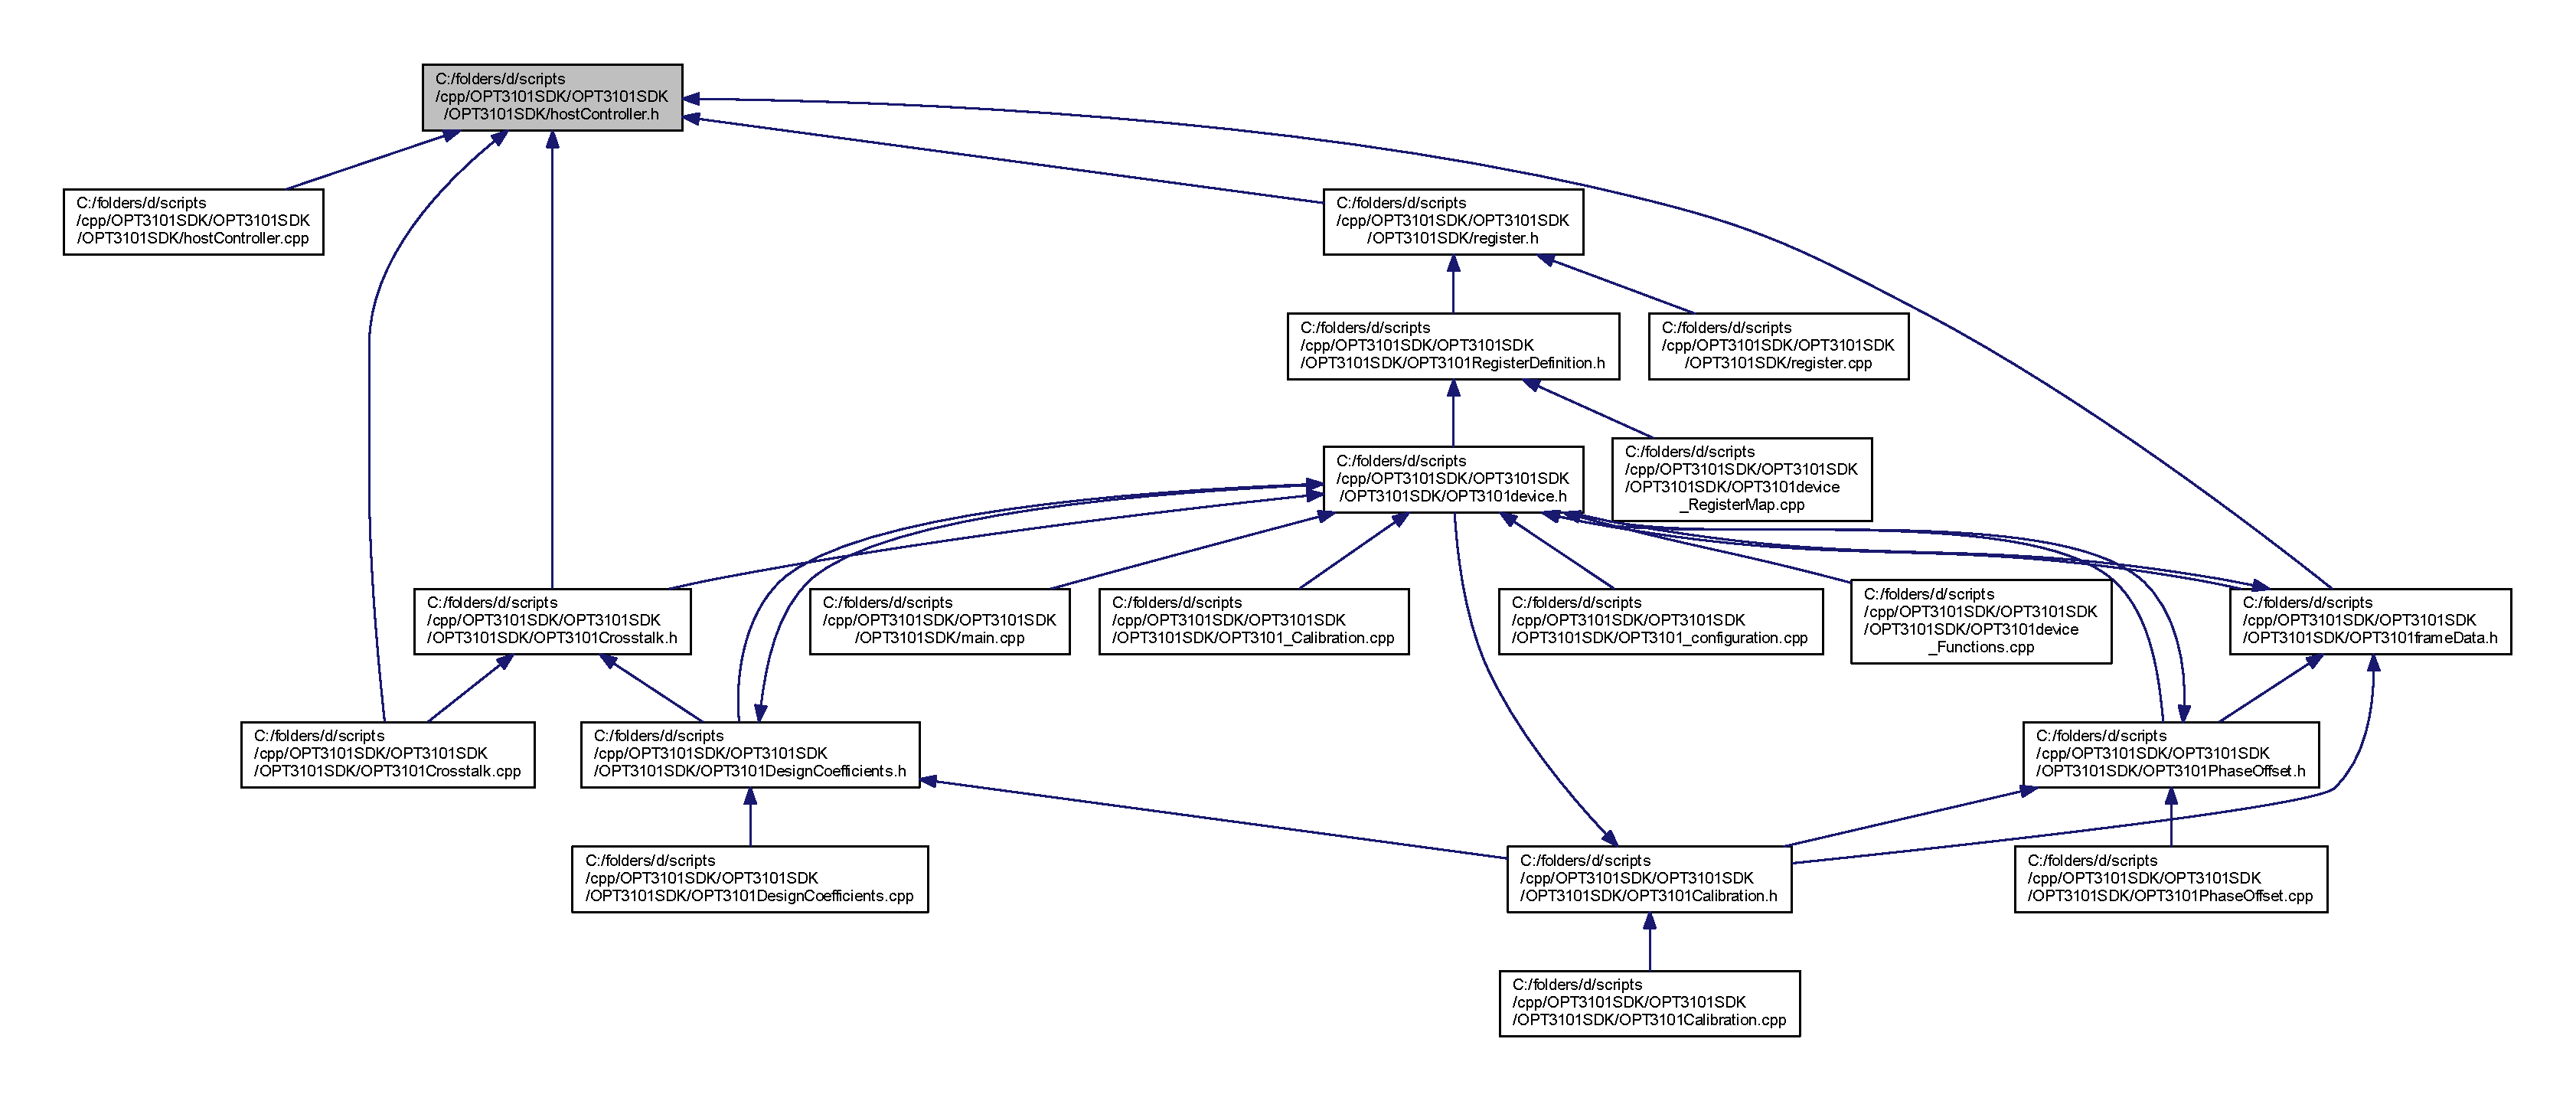
\includegraphics[width=350pt]{host_controller_8h__dep__incl}
\end{center}
\end{figure}
\subsection*{Classes}
\begin{DoxyCompactItemize}
\item 
class \mbox{\hyperlink{classhost_controller}{host\+Controller}}
\begin{DoxyCompactList}\small\item\em Generic implementation for host. \end{DoxyCompactList}\end{DoxyCompactItemize}
\subsection*{Macros}
\begin{DoxyCompactItemize}
\item 
\#define \mbox{\hyperlink{host_controller_8h_a913d77ed1a69aa41135440e6d7e8ec6c}{H\+O\+S\+T\+\_\+\+PC}}
\begin{DoxyCompactList}\small\item\em This pre-\/processor derivative dictates whether the host is PC In a PC environment file storage, std\+::iostream and stdio\+::printf methods are available. All these libraries are enabled then this derivative is defined Disable this derivative in M\+CU or R\+T\+OS like environments where file storage doesn\textquotesingle{}t make sense Disabling this disabled report routines and file storage and load routines. \end{DoxyCompactList}\item 
\#define \mbox{\hyperlink{host_controller_8h_af9ad545b8deb1b3c44ff9168213be470}{O\+P\+T3101\+\_\+\+U\+S\+E\+\_\+\+S\+E\+R\+I\+A\+L\+L\+IB}}
\begin{DoxyCompactList}\small\item\em This pre-\/processor derivative dictates whether to use included \mbox{\hyperlink{serial_8h}{serial.\+h}} library This is enabled by default in S\+DK. Not defining this derivate would disable the serial communication capability. In case of usage with TI E\+VM this derivative is required, if using any other method of communication this can be disabled by user. \end{DoxyCompactList}\item 
\#define \mbox{\hyperlink{host_controller_8h_a3ca6673b36debd7f489557558d93fe38}{O\+P\+T3101\+\_\+\+U\+S\+E\+\_\+\+S\+T\+R\+E\+A\+M\+L\+IB}}
\begin{DoxyCompactList}\small\item\em This pre-\/processor derivative dictates whether to load std\+::iostream and std\+::fstream libraries This is enabled by default in S\+DK. Not defining this derivate would disable all the std\+::iostream and related libraries. File storage will no longer be possible with the S\+DK. All methods related to load\+From\+File and save\+To\+File are hidden to the compiler. \end{DoxyCompactList}\item 
\#define \mbox{\hyperlink{host_controller_8h_a140baa610a82653550ea9aa0a85feb43}{O\+P\+T3101\+\_\+\+U\+S\+E\+\_\+\+S\+T\+D\+I\+O\+L\+IB}}
\begin{DoxyCompactList}\small\item\em This pre-\/processor derivative dictates whether to load stdio library which contains printf and sprintf methods This is enabled by default in S\+DK. Not defining this derivate would disable all sprintf and printf methods. This means that the report() methods on several calls will be blank to the compiler. All file storage is also disabled since the name for the files cannot be resolved without the sprintf method. \end{DoxyCompactList}\item 
\#define \mbox{\hyperlink{host_controller_8h_aa24ee54470842f8fefec2d23f3705a5d}{H\+O\+S\+T\+C\+O\+N\+T\+R\+O\+L\+L\+E\+R\+\_\+\+H\+\_\+}}
\item 
\#define \mbox{\hyperlink{host_controller_8h_a610ce22de673afc7b1e8b0e7b3c9fe7a}{F\+I\+L\+E\+N\+A\+M\+E\+\_\+\+L\+E\+N\+G\+TH}}~50
\end{DoxyCompactItemize}
\subsection*{Variables}
\begin{DoxyCompactItemize}
\item 
\mbox{\hyperlink{classserial_1_1_serial}{serial\+::\+Serial}} \mbox{\hyperlink{host_controller_8h_ad1ec6a8cb3972024759d139433133fee}{O\+P\+T3101command\+Port}}
\begin{DoxyCompactList}\small\item\em Serial Command Port declaration This global variable declaration with name O\+P\+T3101command\+Port of class \mbox{\hyperlink{classserial_1_1_serial}{serial\+::\+Serial}} is used by class like \mbox{\hyperlink{class_o_p_t3101_1_1device_register}{O\+P\+T3101\+::device\+Register}} for I2C read and writes. \end{DoxyCompactList}\item 
const char \mbox{\hyperlink{host_controller_8h_a84ce75d62690cdf4061bfa917ce90bc8}{file\+Path}} \mbox{[}$\,$\mbox{]}
\begin{DoxyCompactList}\small\item\em file\+Path This global variable to declare a path to all calibration files storage \end{DoxyCompactList}\item 
\mbox{\hyperlink{classhost_controller}{host\+Controller}} \mbox{\hyperlink{host_controller_8h_a47f8cbf152e48aa4fdb624be57a9a856}{host}}
\begin{DoxyCompactList}\small\item\em \mbox{\hyperlink{classhost_controller}{host\+Controller}} declaration This global variable declaration with name host of class \mbox{\hyperlink{classhost_controller}{host\+Controller}} is used by various different classes like \mbox{\hyperlink{class_o_p_t3101_1_1device_register}{O\+P\+T3101\+::device\+Register}} , \mbox{\hyperlink{class_o_p_t3101_1_1registers}{O\+P\+T3101\+::registers}} and \mbox{\hyperlink{class_o_p_t3101_1_1device}{O\+P\+T3101\+::device}} to specify specific instructions to the host like wait, sleep, I2C reads and writes \end{DoxyCompactList}\end{DoxyCompactItemize}


\subsection{Detailed Description}
\begin{DoxyAuthor}{Author}
Karthik Rajagopal \href{mailto:krthik@ti.com}{\tt krthik@ti.\+com} 
\end{DoxyAuthor}
\begin{DoxyVersion}{Version}
0.\+8
\end{DoxyVersion}
\hypertarget{register_8h_COPYRIGHT}{}\subsection{C\+O\+P\+Y\+R\+I\+G\+HT}\label{register_8h_COPYRIGHT}
T\+E\+X\+AS I\+N\+S\+T\+R\+U\+M\+E\+N\+TS T\+E\+XT F\+I\+LE L\+I\+C\+E\+N\+SE Copyright (c) 2018 Texas Instruments Incorporated All rights reserved not granted herein. Limited License. Texas Instruments Incorporated grants a world-\/wide, royalty-\/free, non-\/exclusive license under copyrights and patents it now or hereafter owns or controls to make, have made, use, import, offer to sell and sell (\char`\"{}\+Utilize\char`\"{}) this software subject to the terms herein. With respect to the foregoing patent license, such license is granted solely to the extent that any such patent is necessary to Utilize the software alone. The patent license shall not apply to any combinations which include this software, other than combinations with devices manufactured by or for TI (“\+TI Devices”). No hardware patent is licensed hereunder. Redistributions must preserve existing copyright notices and reproduce this license (including the above copyright notice and the disclaimer and (if applicable) source code license limitations below) in the documentation and/or other materials provided with the distribution Redistribution and use in binary form, without modification, are permitted provided that the following conditions are met\+:
\begin{DoxyItemize}
\item No reverse engineering, decompilation, or disassembly of this software is permitted with respect to any software provided in binary form.
\item any redistribution and use are licensed by TI for use only with TI Devices.
\item Nothing shall obligate TI to provide you with source code for the software licensed and provided to you in object code. If software source code is provided to you, modification and redistribution of the source code are permitted provided that the following conditions are met\+:
\item any redistribution and use of the source code, including any resulting derivative works, are licensed by TI for use only with TI Devices.
\item any redistribution and use of any object code compiled from the source code and any resulting derivative works, are licensed by TI for use only with TI Devices. Neither the name of Texas Instruments Incorporated nor the names of its suppliers may be used to endorse or promote products derived from this software without specific prior written permission. D\+I\+S\+C\+L\+A\+I\+M\+ER. T\+H\+IS S\+O\+F\+T\+W\+A\+RE IS P\+R\+O\+V\+I\+D\+ED BY TI A\+ND T\+I’S L\+I\+C\+E\+N\+S\+O\+RS \char`\"{}\+A\+S I\+S\char`\"{} A\+ND A\+NY E\+X\+P\+R\+E\+SS OR I\+M\+P\+L\+I\+ED W\+A\+R\+R\+A\+N\+T\+I\+ES, I\+N\+C\+L\+U\+D\+I\+NG, B\+UT N\+OT L\+I\+M\+I\+T\+ED TO, T\+HE I\+M\+P\+L\+I\+ED W\+A\+R\+R\+A\+N\+T\+I\+ES OF M\+E\+R\+C\+H\+A\+N\+T\+A\+B\+I\+L\+I\+TY A\+ND F\+I\+T\+N\+E\+SS F\+OR A P\+A\+R\+T\+I\+C\+U\+L\+AR P\+U\+R\+P\+O\+SE A\+RE D\+I\+S\+C\+L\+A\+I\+M\+ED. IN NO E\+V\+E\+NT S\+H\+A\+LL TI A\+ND T\+I’S L\+I\+C\+E\+N\+S\+O\+RS BE L\+I\+A\+B\+LE F\+OR A\+NY D\+I\+R\+E\+CT, I\+N\+D\+I\+R\+E\+CT, I\+N\+C\+I\+D\+E\+N\+T\+AL, S\+P\+E\+C\+I\+AL, E\+X\+E\+M\+P\+L\+A\+RY, OR C\+O\+N\+S\+E\+Q\+U\+E\+N\+T\+I\+AL D\+A\+M\+A\+G\+ES (I\+N\+C\+L\+U\+D\+I\+NG, B\+UT N\+OT L\+I\+M\+I\+T\+ED TO, P\+R\+O\+C\+U\+R\+E\+M\+E\+NT OF S\+U\+B\+S\+T\+I\+T\+U\+TE G\+O\+O\+DS OR S\+E\+R\+V\+I\+C\+ES; L\+O\+SS OF U\+SE, D\+A\+TA, OR P\+R\+O\+F\+I\+TS; OR B\+U\+S\+I\+N\+E\+SS I\+N\+T\+E\+R\+R\+U\+P\+T\+I\+ON) H\+O\+W\+E\+V\+ER C\+A\+U\+S\+ED A\+ND ON A\+NY T\+H\+E\+O\+RY OF L\+I\+A\+B\+I\+L\+I\+TY, W\+H\+E\+T\+H\+ER IN C\+O\+N\+T\+R\+A\+CT, S\+T\+R\+I\+CT L\+I\+A\+B\+I\+L\+I\+TY, OR T\+O\+RT (I\+N\+C\+L\+U\+D\+I\+NG N\+E\+G\+L\+I\+G\+E\+N\+CE OR O\+T\+H\+E\+R\+W\+I\+SE) A\+R\+I\+S\+I\+NG IN A\+NY W\+AY O\+UT OF T\+HE U\+SE OF T\+H\+IS S\+O\+F\+T\+W\+A\+RE, E\+V\+EN IF A\+D\+V\+I\+S\+ED OF T\+HE P\+O\+S\+S\+I\+B\+I\+L\+I\+TY OF S\+U\+CH D\+A\+M\+A\+GE.
\end{DoxyItemize}\hypertarget{register_8h_DESCRIPTION}{}\subsection{D\+E\+S\+C\+R\+I\+P\+T\+I\+ON}\label{register_8h_DESCRIPTION}
This file contains the \mbox{\hyperlink{classhost_controller}{host\+Controller}} class. This file contains a general template for a host controller 

\subsection{Macro Definition Documentation}
\mbox{\Hypertarget{host_controller_8h_a610ce22de673afc7b1e8b0e7b3c9fe7a}\label{host_controller_8h_a610ce22de673afc7b1e8b0e7b3c9fe7a}} 
\index{host\+Controller.\+h@{host\+Controller.\+h}!F\+I\+L\+E\+N\+A\+M\+E\+\_\+\+L\+E\+N\+G\+TH@{F\+I\+L\+E\+N\+A\+M\+E\+\_\+\+L\+E\+N\+G\+TH}}
\index{F\+I\+L\+E\+N\+A\+M\+E\+\_\+\+L\+E\+N\+G\+TH@{F\+I\+L\+E\+N\+A\+M\+E\+\_\+\+L\+E\+N\+G\+TH}!host\+Controller.\+h@{host\+Controller.\+h}}
\subsubsection{\texorpdfstring{F\+I\+L\+E\+N\+A\+M\+E\+\_\+\+L\+E\+N\+G\+TH}{FILENAME\_LENGTH}}
{\footnotesize\ttfamily \#define F\+I\+L\+E\+N\+A\+M\+E\+\_\+\+L\+E\+N\+G\+TH~50}

\mbox{\Hypertarget{host_controller_8h_a913d77ed1a69aa41135440e6d7e8ec6c}\label{host_controller_8h_a913d77ed1a69aa41135440e6d7e8ec6c}} 
\index{host\+Controller.\+h@{host\+Controller.\+h}!H\+O\+S\+T\+\_\+\+PC@{H\+O\+S\+T\+\_\+\+PC}}
\index{H\+O\+S\+T\+\_\+\+PC@{H\+O\+S\+T\+\_\+\+PC}!host\+Controller.\+h@{host\+Controller.\+h}}
\subsubsection{\texorpdfstring{H\+O\+S\+T\+\_\+\+PC}{HOST\_PC}}
{\footnotesize\ttfamily \#define H\+O\+S\+T\+\_\+\+PC}



This pre-\/processor derivative dictates whether the host is PC In a PC environment file storage, std\+::iostream and stdio\+::printf methods are available. All these libraries are enabled then this derivative is defined Disable this derivative in M\+CU or R\+T\+OS like environments where file storage doesn\textquotesingle{}t make sense Disabling this disabled report routines and file storage and load routines. 

\mbox{\Hypertarget{host_controller_8h_aa24ee54470842f8fefec2d23f3705a5d}\label{host_controller_8h_aa24ee54470842f8fefec2d23f3705a5d}} 
\index{host\+Controller.\+h@{host\+Controller.\+h}!H\+O\+S\+T\+C\+O\+N\+T\+R\+O\+L\+L\+E\+R\+\_\+\+H\+\_\+@{H\+O\+S\+T\+C\+O\+N\+T\+R\+O\+L\+L\+E\+R\+\_\+\+H\+\_\+}}
\index{H\+O\+S\+T\+C\+O\+N\+T\+R\+O\+L\+L\+E\+R\+\_\+\+H\+\_\+@{H\+O\+S\+T\+C\+O\+N\+T\+R\+O\+L\+L\+E\+R\+\_\+\+H\+\_\+}!host\+Controller.\+h@{host\+Controller.\+h}}
\subsubsection{\texorpdfstring{H\+O\+S\+T\+C\+O\+N\+T\+R\+O\+L\+L\+E\+R\+\_\+\+H\+\_\+}{HOSTCONTROLLER\_H\_}}
{\footnotesize\ttfamily \#define H\+O\+S\+T\+C\+O\+N\+T\+R\+O\+L\+L\+E\+R\+\_\+\+H\+\_\+}

\mbox{\Hypertarget{host_controller_8h_af9ad545b8deb1b3c44ff9168213be470}\label{host_controller_8h_af9ad545b8deb1b3c44ff9168213be470}} 
\index{host\+Controller.\+h@{host\+Controller.\+h}!O\+P\+T3101\+\_\+\+U\+S\+E\+\_\+\+S\+E\+R\+I\+A\+L\+L\+IB@{O\+P\+T3101\+\_\+\+U\+S\+E\+\_\+\+S\+E\+R\+I\+A\+L\+L\+IB}}
\index{O\+P\+T3101\+\_\+\+U\+S\+E\+\_\+\+S\+E\+R\+I\+A\+L\+L\+IB@{O\+P\+T3101\+\_\+\+U\+S\+E\+\_\+\+S\+E\+R\+I\+A\+L\+L\+IB}!host\+Controller.\+h@{host\+Controller.\+h}}
\subsubsection{\texorpdfstring{O\+P\+T3101\+\_\+\+U\+S\+E\+\_\+\+S\+E\+R\+I\+A\+L\+L\+IB}{OPT3101\_USE\_SERIALLIB}}
{\footnotesize\ttfamily \#define O\+P\+T3101\+\_\+\+U\+S\+E\+\_\+\+S\+E\+R\+I\+A\+L\+L\+IB}



This pre-\/processor derivative dictates whether to use included \mbox{\hyperlink{serial_8h}{serial.\+h}} library This is enabled by default in S\+DK. Not defining this derivate would disable the serial communication capability. In case of usage with TI E\+VM this derivative is required, if using any other method of communication this can be disabled by user. 

\mbox{\Hypertarget{host_controller_8h_a140baa610a82653550ea9aa0a85feb43}\label{host_controller_8h_a140baa610a82653550ea9aa0a85feb43}} 
\index{host\+Controller.\+h@{host\+Controller.\+h}!O\+P\+T3101\+\_\+\+U\+S\+E\+\_\+\+S\+T\+D\+I\+O\+L\+IB@{O\+P\+T3101\+\_\+\+U\+S\+E\+\_\+\+S\+T\+D\+I\+O\+L\+IB}}
\index{O\+P\+T3101\+\_\+\+U\+S\+E\+\_\+\+S\+T\+D\+I\+O\+L\+IB@{O\+P\+T3101\+\_\+\+U\+S\+E\+\_\+\+S\+T\+D\+I\+O\+L\+IB}!host\+Controller.\+h@{host\+Controller.\+h}}
\subsubsection{\texorpdfstring{O\+P\+T3101\+\_\+\+U\+S\+E\+\_\+\+S\+T\+D\+I\+O\+L\+IB}{OPT3101\_USE\_STDIOLIB}}
{\footnotesize\ttfamily \#define O\+P\+T3101\+\_\+\+U\+S\+E\+\_\+\+S\+T\+D\+I\+O\+L\+IB}



This pre-\/processor derivative dictates whether to load stdio library which contains printf and sprintf methods This is enabled by default in S\+DK. Not defining this derivate would disable all sprintf and printf methods. This means that the report() methods on several calls will be blank to the compiler. All file storage is also disabled since the name for the files cannot be resolved without the sprintf method. 

\mbox{\Hypertarget{host_controller_8h_a3ca6673b36debd7f489557558d93fe38}\label{host_controller_8h_a3ca6673b36debd7f489557558d93fe38}} 
\index{host\+Controller.\+h@{host\+Controller.\+h}!O\+P\+T3101\+\_\+\+U\+S\+E\+\_\+\+S\+T\+R\+E\+A\+M\+L\+IB@{O\+P\+T3101\+\_\+\+U\+S\+E\+\_\+\+S\+T\+R\+E\+A\+M\+L\+IB}}
\index{O\+P\+T3101\+\_\+\+U\+S\+E\+\_\+\+S\+T\+R\+E\+A\+M\+L\+IB@{O\+P\+T3101\+\_\+\+U\+S\+E\+\_\+\+S\+T\+R\+E\+A\+M\+L\+IB}!host\+Controller.\+h@{host\+Controller.\+h}}
\subsubsection{\texorpdfstring{O\+P\+T3101\+\_\+\+U\+S\+E\+\_\+\+S\+T\+R\+E\+A\+M\+L\+IB}{OPT3101\_USE\_STREAMLIB}}
{\footnotesize\ttfamily \#define O\+P\+T3101\+\_\+\+U\+S\+E\+\_\+\+S\+T\+R\+E\+A\+M\+L\+IB}



This pre-\/processor derivative dictates whether to load std\+::iostream and std\+::fstream libraries This is enabled by default in S\+DK. Not defining this derivate would disable all the std\+::iostream and related libraries. File storage will no longer be possible with the S\+DK. All methods related to load\+From\+File and save\+To\+File are hidden to the compiler. 



\subsection{Variable Documentation}
\mbox{\Hypertarget{host_controller_8h_a84ce75d62690cdf4061bfa917ce90bc8}\label{host_controller_8h_a84ce75d62690cdf4061bfa917ce90bc8}} 
\index{host\+Controller.\+h@{host\+Controller.\+h}!file\+Path@{file\+Path}}
\index{file\+Path@{file\+Path}!host\+Controller.\+h@{host\+Controller.\+h}}
\subsubsection{\texorpdfstring{file\+Path}{filePath}}
{\footnotesize\ttfamily const char file\+Path\mbox{[}$\,$\mbox{]}}



file\+Path This global variable to declare a path to all calibration files storage 

\mbox{\Hypertarget{host_controller_8h_a47f8cbf152e48aa4fdb624be57a9a856}\label{host_controller_8h_a47f8cbf152e48aa4fdb624be57a9a856}} 
\index{host\+Controller.\+h@{host\+Controller.\+h}!host@{host}}
\index{host@{host}!host\+Controller.\+h@{host\+Controller.\+h}}
\subsubsection{\texorpdfstring{host}{host}}
{\footnotesize\ttfamily \mbox{\hyperlink{classhost_controller}{host\+Controller}} host}



\mbox{\hyperlink{classhost_controller}{host\+Controller}} declaration This global variable declaration with name host of class \mbox{\hyperlink{classhost_controller}{host\+Controller}} is used by various different classes like \mbox{\hyperlink{class_o_p_t3101_1_1device_register}{O\+P\+T3101\+::device\+Register}} , \mbox{\hyperlink{class_o_p_t3101_1_1registers}{O\+P\+T3101\+::registers}} and \mbox{\hyperlink{class_o_p_t3101_1_1device}{O\+P\+T3101\+::device}} to specify specific instructions to the host like wait, sleep, I2C reads and writes 

\mbox{\Hypertarget{host_controller_8h_ad1ec6a8cb3972024759d139433133fee}\label{host_controller_8h_ad1ec6a8cb3972024759d139433133fee}} 
\index{host\+Controller.\+h@{host\+Controller.\+h}!O\+P\+T3101command\+Port@{O\+P\+T3101command\+Port}}
\index{O\+P\+T3101command\+Port@{O\+P\+T3101command\+Port}!host\+Controller.\+h@{host\+Controller.\+h}}
\subsubsection{\texorpdfstring{O\+P\+T3101command\+Port}{OPT3101commandPort}}
{\footnotesize\ttfamily \mbox{\hyperlink{classserial_1_1_serial}{serial\+::\+Serial}} O\+P\+T3101command\+Port}



Serial Command Port declaration This global variable declaration with name O\+P\+T3101command\+Port of class \mbox{\hyperlink{classserial_1_1_serial}{serial\+::\+Serial}} is used by class like \mbox{\hyperlink{class_o_p_t3101_1_1device_register}{O\+P\+T3101\+::device\+Register}} for I2C read and writes. 


\hypertarget{main_8cpp}{}\section{C\+:/folders/d/scripts/cpp/\+O\+P\+T3101\+S\+D\+K/\+O\+P\+T3101\+S\+D\+K/\+O\+P\+T3101\+S\+D\+K/main.cpp File Reference}
\label{main_8cpp}\index{C\+:/folders/d/scripts/cpp/\+O\+P\+T3101\+S\+D\+K/\+O\+P\+T3101\+S\+D\+K/\+O\+P\+T3101\+S\+D\+K/main.\+cpp@{C\+:/folders/d/scripts/cpp/\+O\+P\+T3101\+S\+D\+K/\+O\+P\+T3101\+S\+D\+K/\+O\+P\+T3101\+S\+D\+K/main.\+cpp}}
{\ttfamily \#include $<$stdio.\+h$>$}\newline
{\ttfamily \#include \char`\"{}O\+P\+T3101device.\+h\char`\"{}}\newline
Include dependency graph for main.\+cpp\+:\nopagebreak
\begin{figure}[H]
\begin{center}
\leavevmode
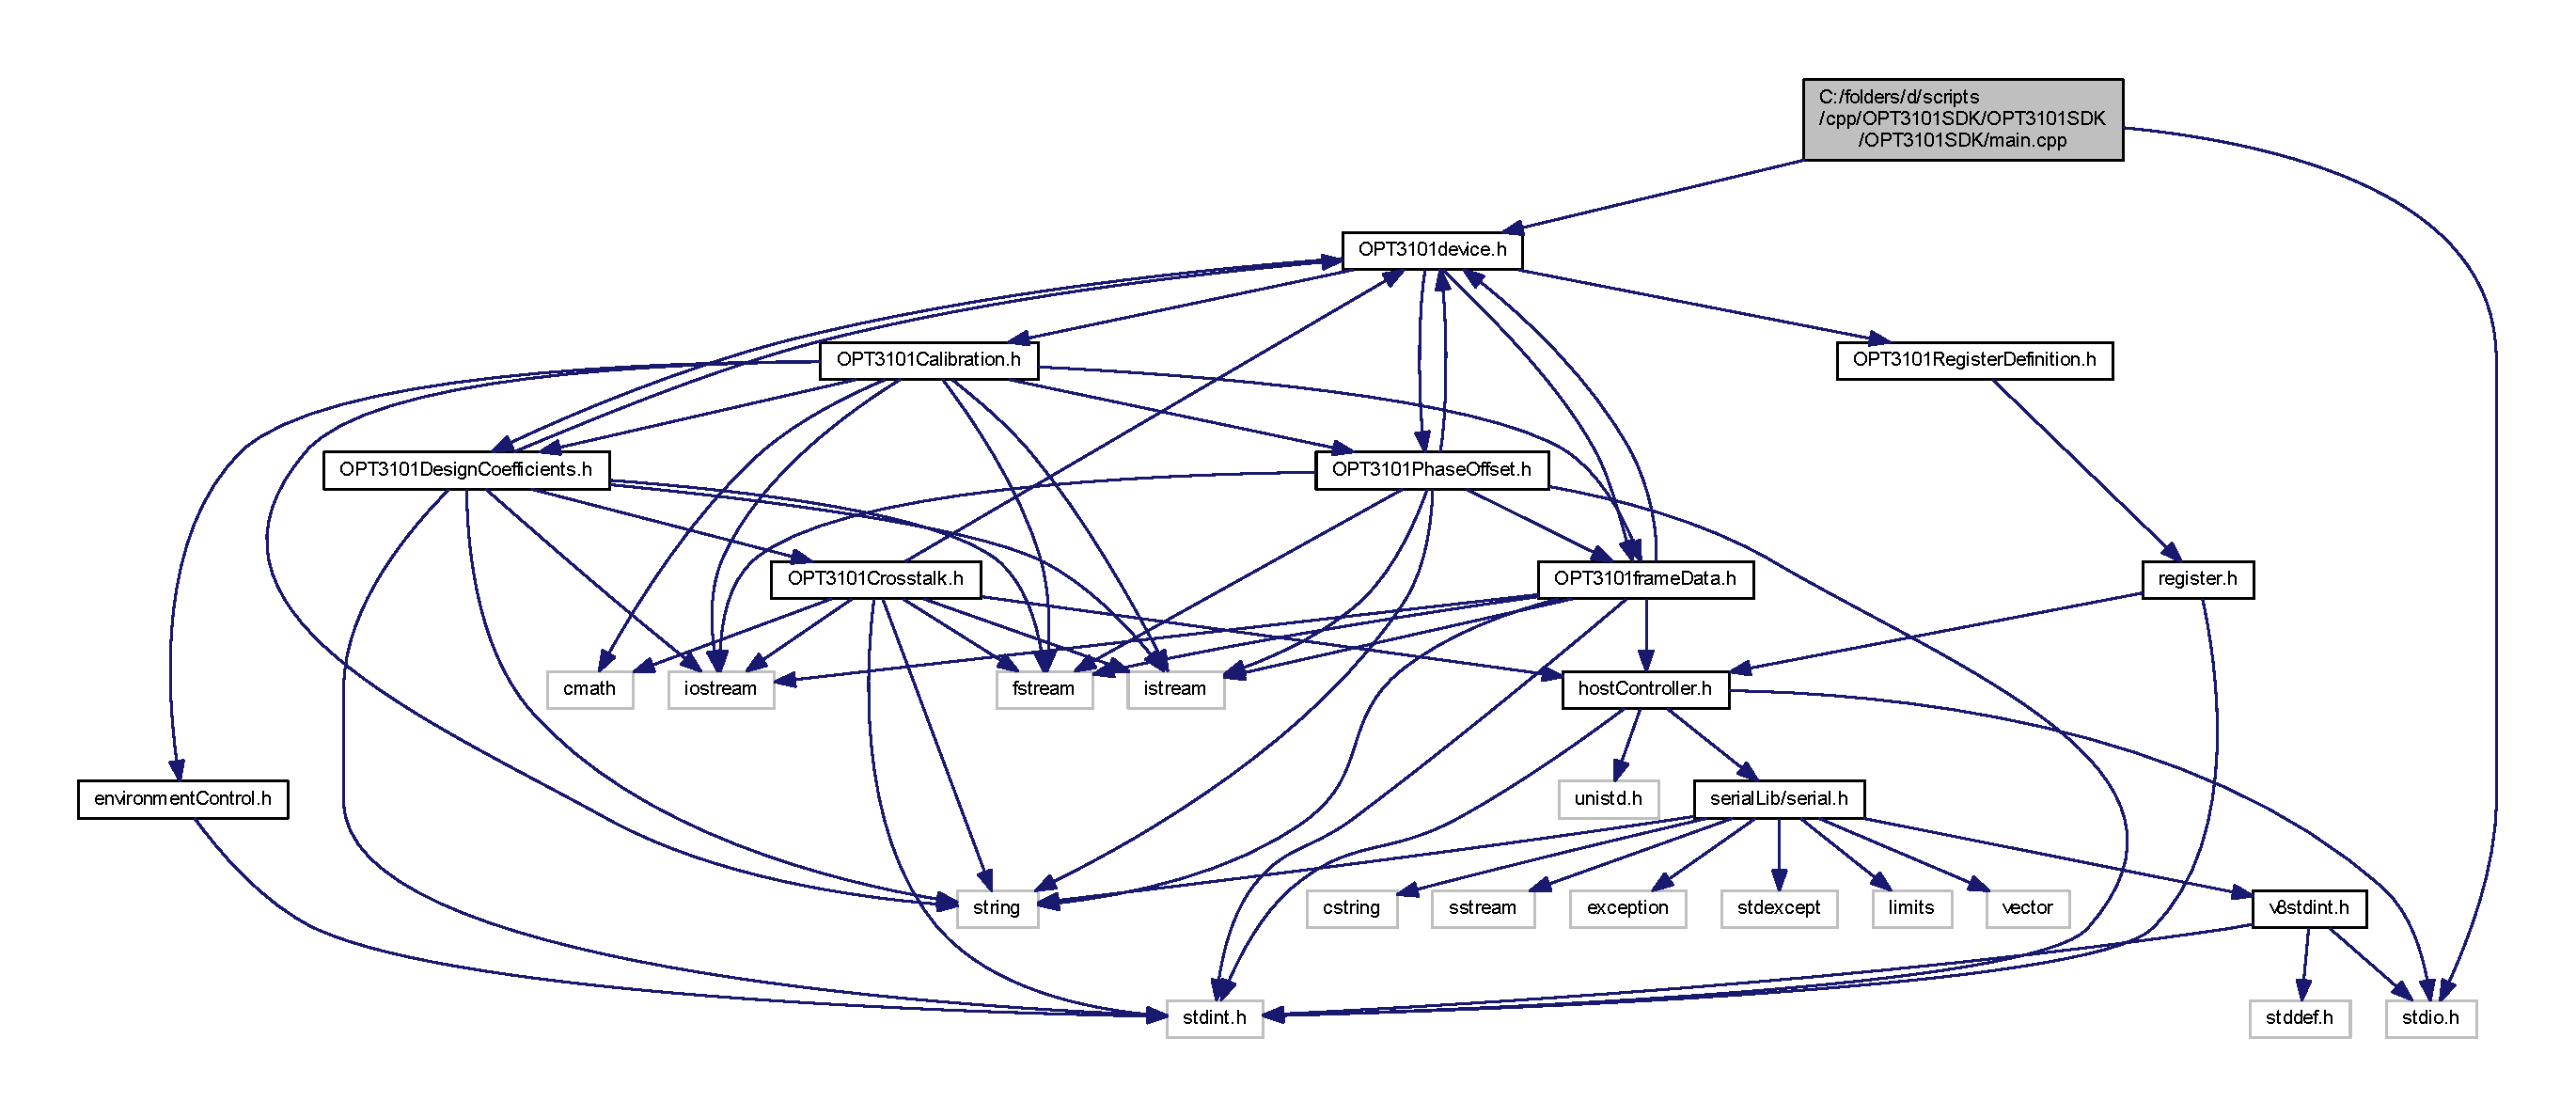
\includegraphics[width=350pt]{main_8cpp__incl}
\end{center}
\end{figure}
\subsection*{Functions}
\begin{DoxyCompactItemize}
\item 
int \mbox{\hyperlink{main_8cpp_ae66f6b31b5ad750f1fe042a706a4e3d4}{main}} ()
\end{DoxyCompactItemize}


\subsection{Function Documentation}
\mbox{\Hypertarget{main_8cpp_ae66f6b31b5ad750f1fe042a706a4e3d4}\label{main_8cpp_ae66f6b31b5ad750f1fe042a706a4e3d4}} 
\index{main.\+cpp@{main.\+cpp}!main@{main}}
\index{main@{main}!main.\+cpp@{main.\+cpp}}
\subsubsection{\texorpdfstring{main()}{main()}}
{\footnotesize\ttfamily int main (\begin{DoxyParamCaption}\item[{void}]{ }\end{DoxyParamCaption})}


\begin{DoxyItemize}
\item Declared variable dev of class \mbox{\hyperlink{class_o_p_t3101_1_1device}{O\+P\+T3101\+::device}} ~\newline
~\newline
~\newline

\item Calls the method to bring up the device first time and calibrate. Calls O\+P\+T3101\+::calibration\+Session\+\_\+first\+Time\+Bring\+Up
\item Calls report function for all calibration coefficients. Since not all coefficients are done in this example most of them are expected to be zero.
\item Waits for user input before closing the console 
\end{DoxyItemize}
\hypertarget{serial_lib_2main_8cpp}{}\section{C\+:/folders/d/scripts/cpp/\+O\+P\+T3101\+S\+D\+K/\+O\+P\+T3101\+S\+D\+K/\+O\+P\+T3101\+S\+D\+K/serial\+Lib/main.cpp File Reference}
\label{serial_lib_2main_8cpp}\index{C\+:/folders/d/scripts/cpp/\+O\+P\+T3101\+S\+D\+K/\+O\+P\+T3101\+S\+D\+K/\+O\+P\+T3101\+S\+D\+K/serial\+Lib/main.\+cpp@{C\+:/folders/d/scripts/cpp/\+O\+P\+T3101\+S\+D\+K/\+O\+P\+T3101\+S\+D\+K/\+O\+P\+T3101\+S\+D\+K/serial\+Lib/main.\+cpp}}
{\ttfamily \#include $<$string$>$}\newline
{\ttfamily \#include $<$iostream$>$}\newline
{\ttfamily \#include $<$cstdio$>$}\newline
{\ttfamily \#include $<$stdio.\+h$>$}\newline
{\ttfamily \#include $<$stdint.\+h$>$}\newline
{\ttfamily \#include $<$stdlib.\+h$>$}\newline
{\ttfamily \#include $<$unistd.\+h$>$}\newline
{\ttfamily \#include \char`\"{}serial.\+h\char`\"{}}\newline
Include dependency graph for main.\+cpp\+:\nopagebreak
\begin{figure}[H]
\begin{center}
\leavevmode
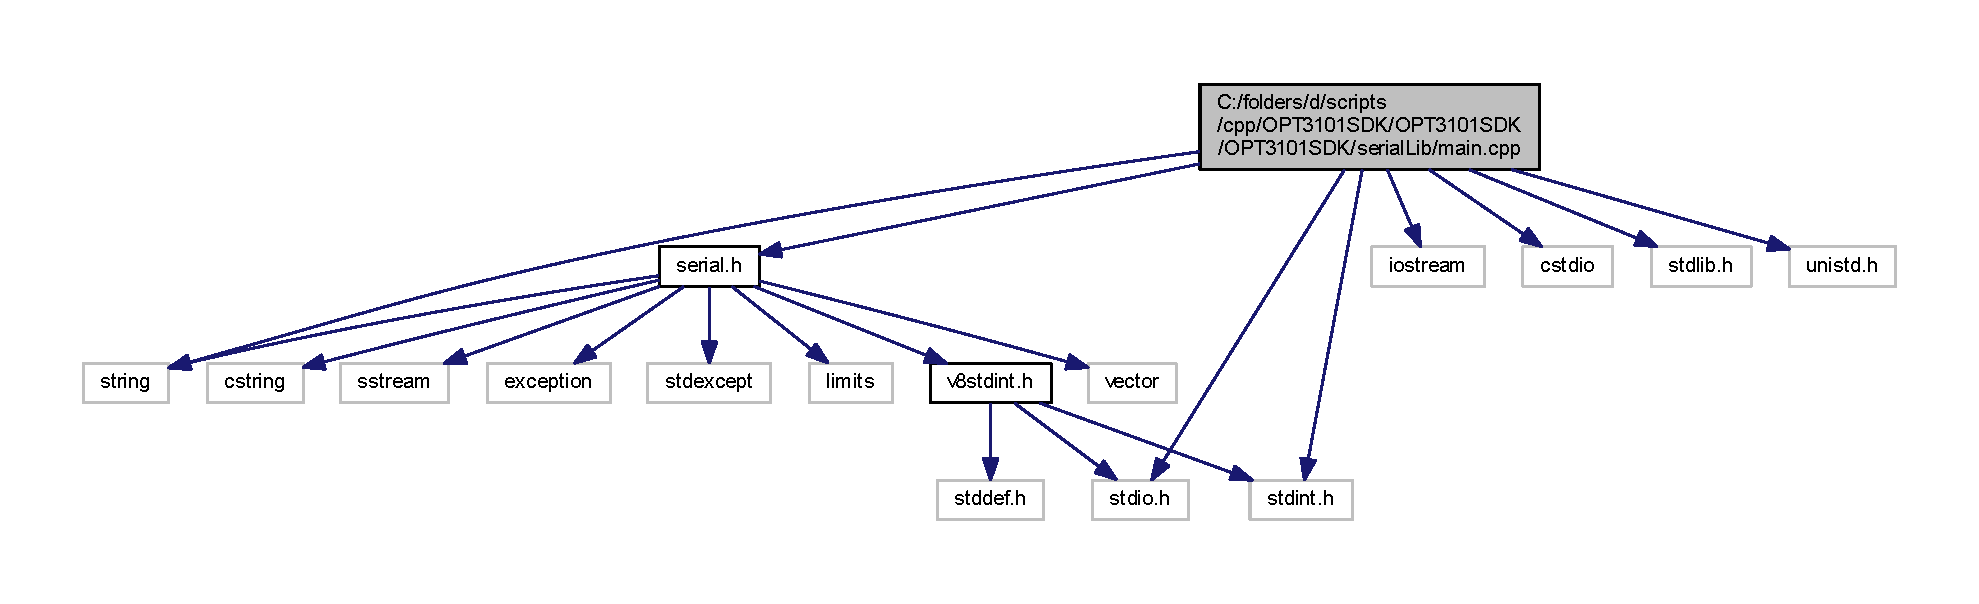
\includegraphics[width=350pt]{serial_lib_2main_8cpp__incl}
\end{center}
\end{figure}
\subsection*{Functions}
\begin{DoxyCompactItemize}
\item 
void \mbox{\hyperlink{serial_lib_2main_8cpp_a89b7c9d8c710b057346cc9ac52ae3734}{my\+\_\+sleep}} (unsigned long milliseconds)
\item 
void \mbox{\hyperlink{serial_lib_2main_8cpp_a996e0d351ea6c804947e9533581765ea}{enumerate\+\_\+ports}} ()
\item 
void \mbox{\hyperlink{serial_lib_2main_8cpp_ae5ad5cbeccaedc03a48d3c7eaa803e79}{print\+\_\+usage}} ()
\item 
int \mbox{\hyperlink{serial_lib_2main_8cpp_ac1f545534cdaab9094198a5dc2c2a79f}{run}} (int argc, char $\ast$$\ast$argv)
\item 
int \mbox{\hyperlink{serial_lib_2main_8cpp_a840291bc02cba5474a4cb46a9b9566fe}{main}} (void)
\end{DoxyCompactItemize}


\subsection{Function Documentation}
\mbox{\Hypertarget{serial_lib_2main_8cpp_a996e0d351ea6c804947e9533581765ea}\label{serial_lib_2main_8cpp_a996e0d351ea6c804947e9533581765ea}} 
\index{serial\+Lib/main.\+cpp@{serial\+Lib/main.\+cpp}!enumerate\+\_\+ports@{enumerate\+\_\+ports}}
\index{enumerate\+\_\+ports@{enumerate\+\_\+ports}!serial\+Lib/main.\+cpp@{serial\+Lib/main.\+cpp}}
\subsubsection{\texorpdfstring{enumerate\+\_\+ports()}{enumerate\_ports()}}
{\footnotesize\ttfamily void enumerate\+\_\+ports (\begin{DoxyParamCaption}{ }\end{DoxyParamCaption})}

\mbox{\Hypertarget{serial_lib_2main_8cpp_a840291bc02cba5474a4cb46a9b9566fe}\label{serial_lib_2main_8cpp_a840291bc02cba5474a4cb46a9b9566fe}} 
\index{serial\+Lib/main.\+cpp@{serial\+Lib/main.\+cpp}!main@{main}}
\index{main@{main}!serial\+Lib/main.\+cpp@{serial\+Lib/main.\+cpp}}
\subsubsection{\texorpdfstring{main()}{main()}}
{\footnotesize\ttfamily int main (\begin{DoxyParamCaption}\item[{void}]{ }\end{DoxyParamCaption})}

\mbox{\Hypertarget{serial_lib_2main_8cpp_a89b7c9d8c710b057346cc9ac52ae3734}\label{serial_lib_2main_8cpp_a89b7c9d8c710b057346cc9ac52ae3734}} 
\index{serial\+Lib/main.\+cpp@{serial\+Lib/main.\+cpp}!my\+\_\+sleep@{my\+\_\+sleep}}
\index{my\+\_\+sleep@{my\+\_\+sleep}!serial\+Lib/main.\+cpp@{serial\+Lib/main.\+cpp}}
\subsubsection{\texorpdfstring{my\+\_\+sleep()}{my\_sleep()}}
{\footnotesize\ttfamily void my\+\_\+sleep (\begin{DoxyParamCaption}\item[{unsigned long}]{milliseconds }\end{DoxyParamCaption})}

\mbox{\Hypertarget{serial_lib_2main_8cpp_ae5ad5cbeccaedc03a48d3c7eaa803e79}\label{serial_lib_2main_8cpp_ae5ad5cbeccaedc03a48d3c7eaa803e79}} 
\index{serial\+Lib/main.\+cpp@{serial\+Lib/main.\+cpp}!print\+\_\+usage@{print\+\_\+usage}}
\index{print\+\_\+usage@{print\+\_\+usage}!serial\+Lib/main.\+cpp@{serial\+Lib/main.\+cpp}}
\subsubsection{\texorpdfstring{print\+\_\+usage()}{print\_usage()}}
{\footnotesize\ttfamily void print\+\_\+usage (\begin{DoxyParamCaption}{ }\end{DoxyParamCaption})}

\mbox{\Hypertarget{serial_lib_2main_8cpp_ac1f545534cdaab9094198a5dc2c2a79f}\label{serial_lib_2main_8cpp_ac1f545534cdaab9094198a5dc2c2a79f}} 
\index{serial\+Lib/main.\+cpp@{serial\+Lib/main.\+cpp}!run@{run}}
\index{run@{run}!serial\+Lib/main.\+cpp@{serial\+Lib/main.\+cpp}}
\subsubsection{\texorpdfstring{run()}{run()}}
{\footnotesize\ttfamily int run (\begin{DoxyParamCaption}\item[{int}]{argc,  }\item[{char $\ast$$\ast$}]{argv }\end{DoxyParamCaption})}


\hypertarget{_o_p_t3101___calibration_8cpp}{}\section{C\+:/folders/d/scripts/cpp/\+O\+P\+T3101\+S\+D\+K/\+O\+P\+T3101\+S\+D\+K/\+O\+P\+T3101\+S\+D\+K/\+O\+P\+T3101\+\_\+\+Calibration.cpp File Reference}
\label{_o_p_t3101___calibration_8cpp}\index{C\+:/folders/d/scripts/cpp/\+O\+P\+T3101\+S\+D\+K/\+O\+P\+T3101\+S\+D\+K/\+O\+P\+T3101\+S\+D\+K/\+O\+P\+T3101\+\_\+\+Calibration.\+cpp@{C\+:/folders/d/scripts/cpp/\+O\+P\+T3101\+S\+D\+K/\+O\+P\+T3101\+S\+D\+K/\+O\+P\+T3101\+S\+D\+K/\+O\+P\+T3101\+\_\+\+Calibration.\+cpp}}
{\ttfamily \#include \char`\"{}O\+P\+T3101device.\+h\char`\"{}}\newline
Include dependency graph for O\+P\+T3101\+\_\+\+Calibration.\+cpp\+:\nopagebreak
\begin{figure}[H]
\begin{center}
\leavevmode
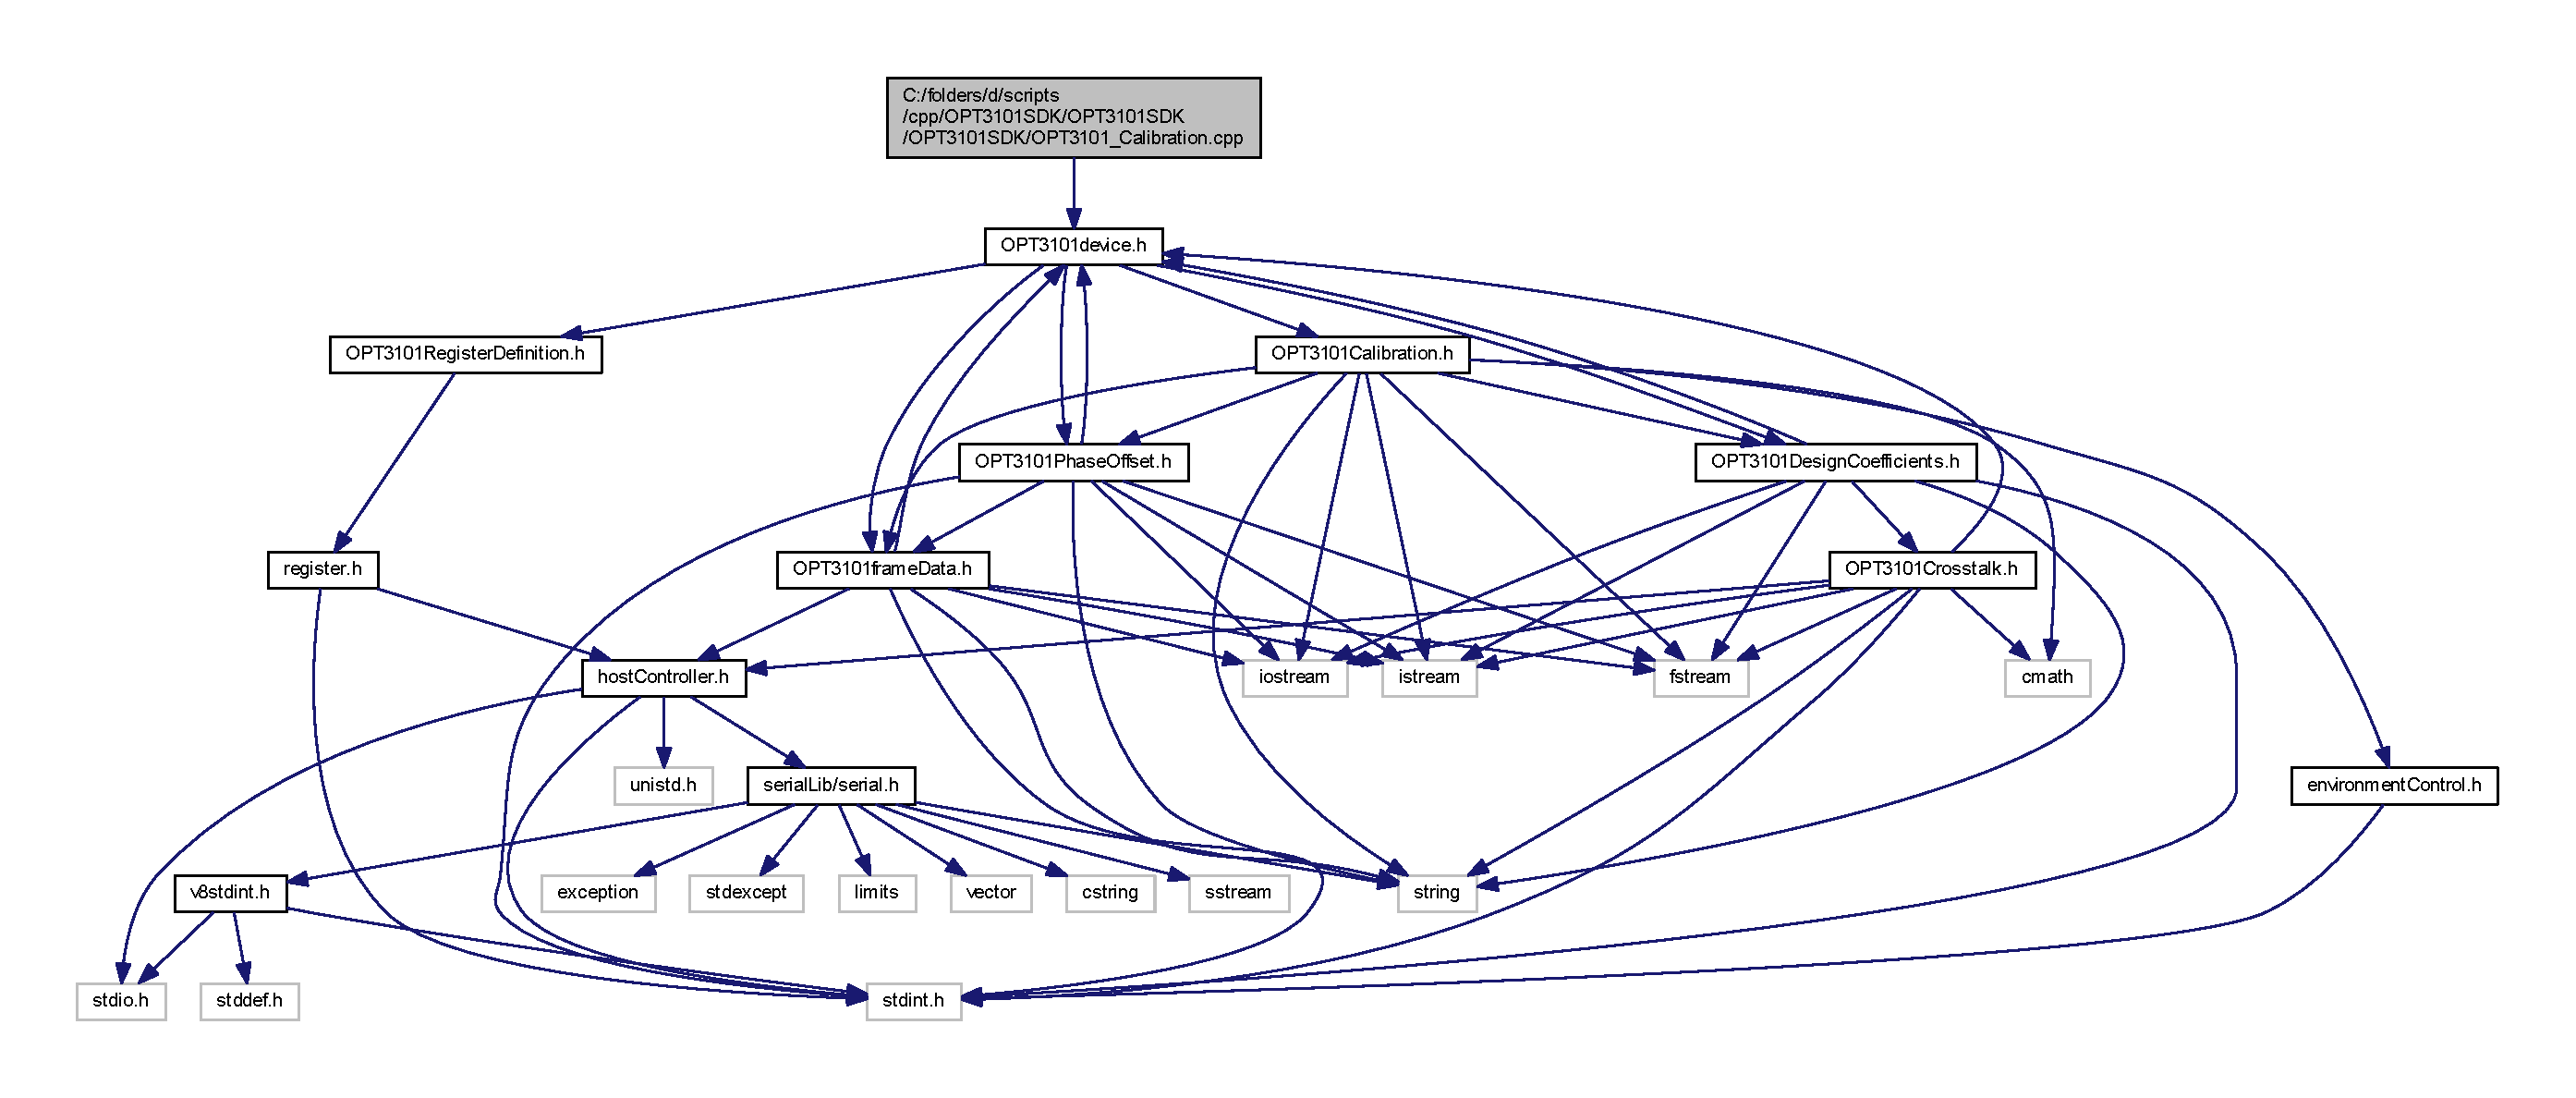
\includegraphics[width=350pt]{_o_p_t3101___calibration_8cpp__incl}
\end{center}
\end{figure}

\hypertarget{_o_p_t3101__configuration_8cpp}{}\section{C\+:/folders/d/scripts/cpp/\+O\+P\+T3101\+S\+D\+K/\+O\+P\+T3101\+S\+D\+K/\+O\+P\+T3101\+S\+D\+K/\+O\+P\+T3101\+\_\+configuration.cpp File Reference}
\label{_o_p_t3101__configuration_8cpp}\index{C\+:/folders/d/scripts/cpp/\+O\+P\+T3101\+S\+D\+K/\+O\+P\+T3101\+S\+D\+K/\+O\+P\+T3101\+S\+D\+K/\+O\+P\+T3101\+\_\+configuration.\+cpp@{C\+:/folders/d/scripts/cpp/\+O\+P\+T3101\+S\+D\+K/\+O\+P\+T3101\+S\+D\+K/\+O\+P\+T3101\+S\+D\+K/\+O\+P\+T3101\+\_\+configuration.\+cpp}}
{\ttfamily \#include \char`\"{}O\+P\+T3101device.\+h\char`\"{}}\newline
Include dependency graph for O\+P\+T3101\+\_\+configuration.\+cpp\+:\nopagebreak
\begin{figure}[H]
\begin{center}
\leavevmode
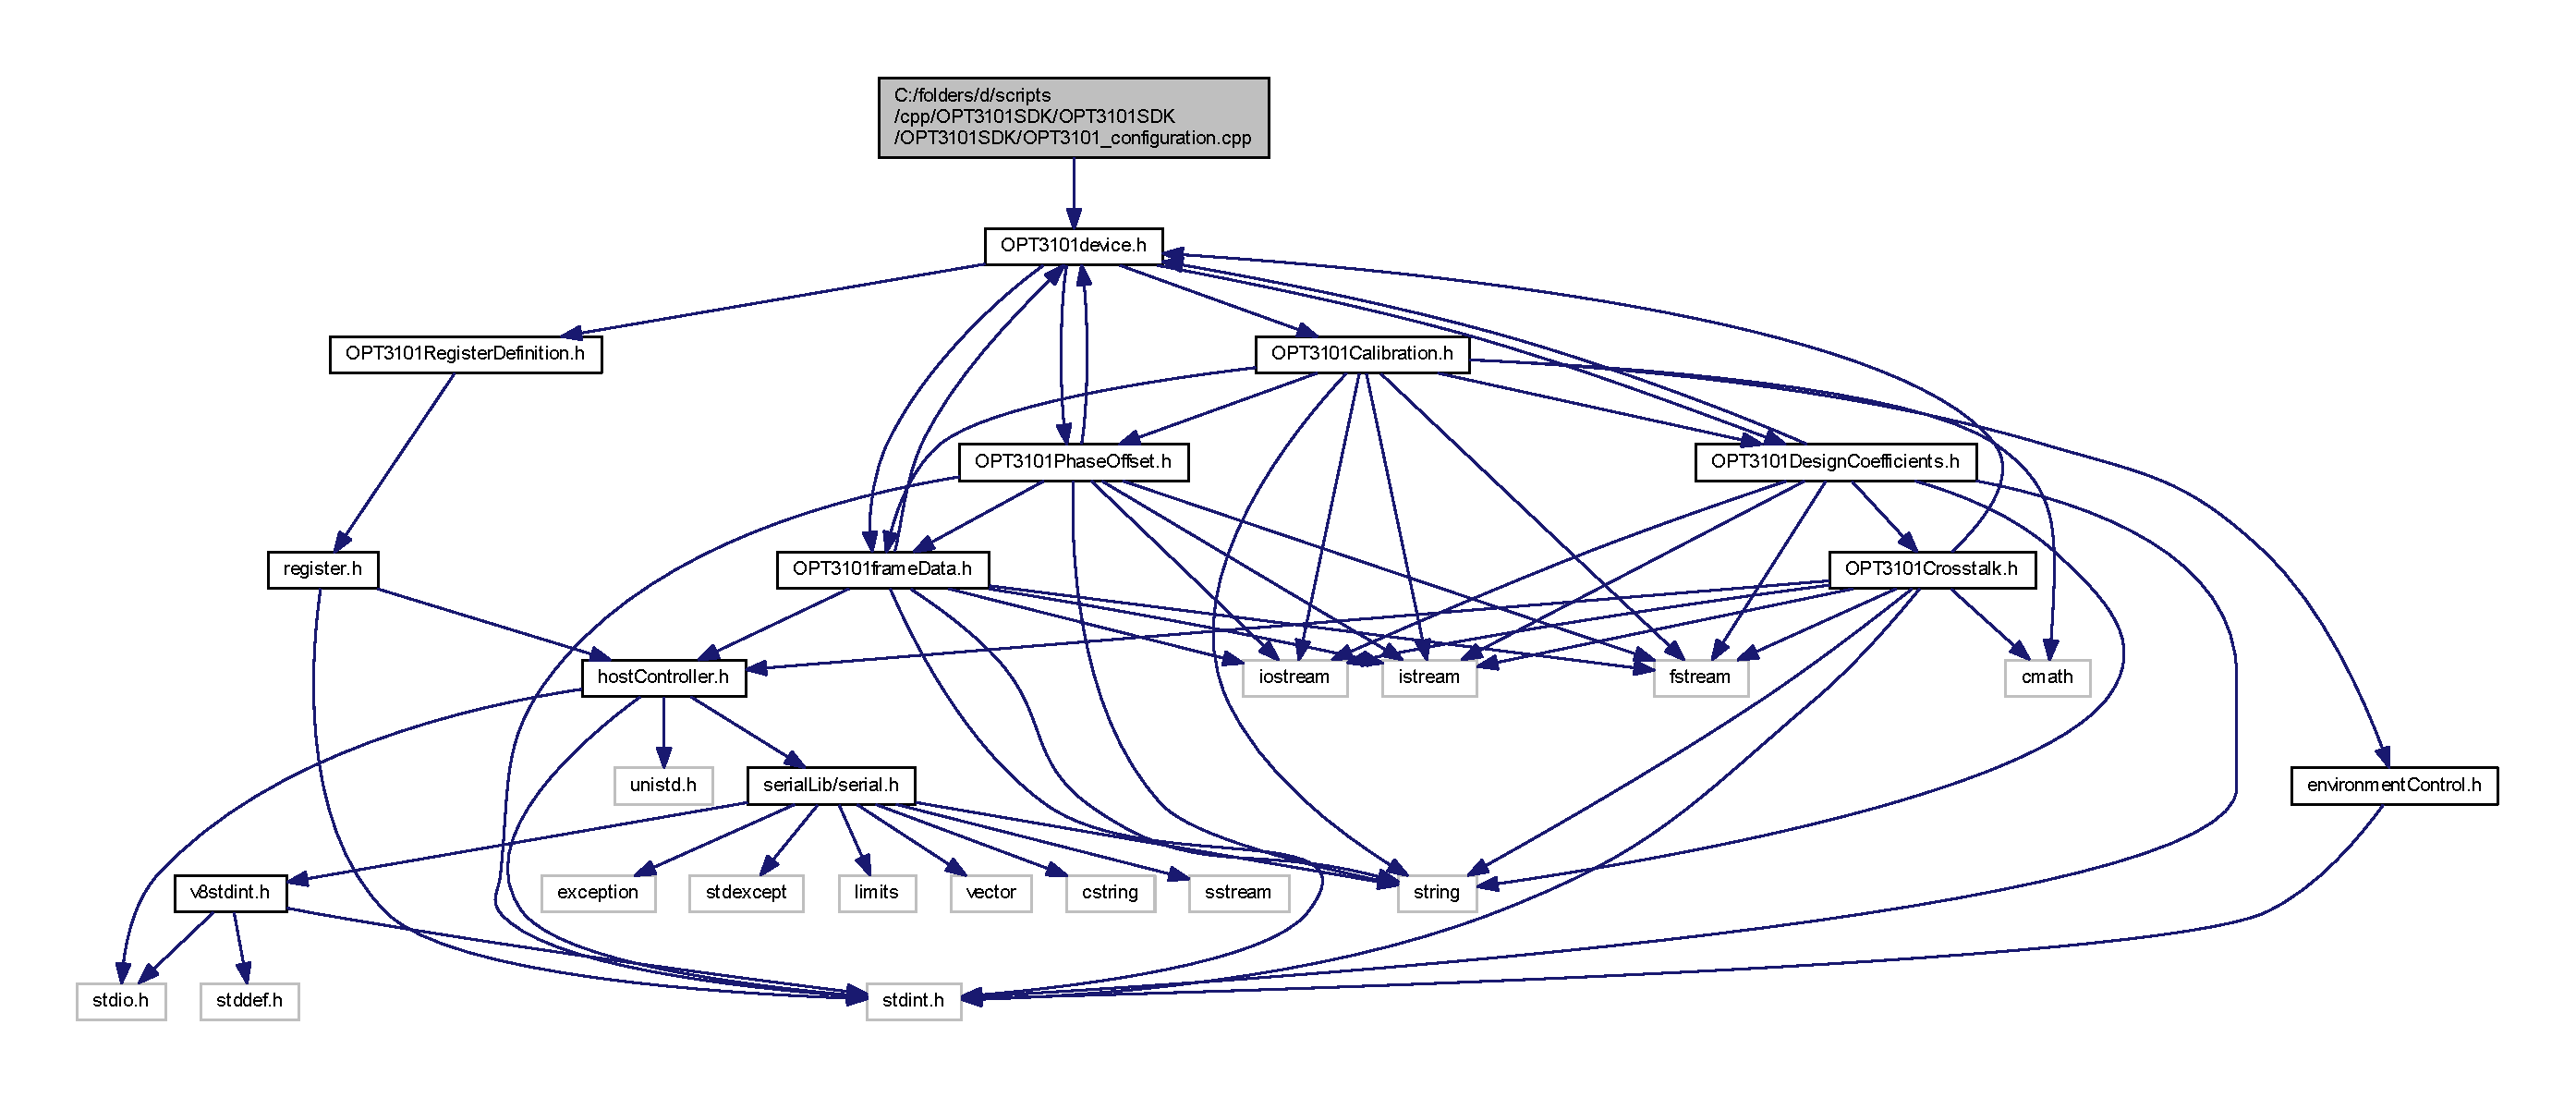
\includegraphics[width=350pt]{_o_p_t3101__configuration_8cpp__incl}
\end{center}
\end{figure}

\hypertarget{_o_p_t3101_calibration_8cpp}{}\section{C\+:/folders/d/scripts/cpp/\+O\+P\+T3101\+S\+D\+K/\+O\+P\+T3101\+S\+D\+K/\+O\+P\+T3101\+S\+D\+K/\+O\+P\+T3101\+Calibration.cpp File Reference}
\label{_o_p_t3101_calibration_8cpp}\index{C\+:/folders/d/scripts/cpp/\+O\+P\+T3101\+S\+D\+K/\+O\+P\+T3101\+S\+D\+K/\+O\+P\+T3101\+S\+D\+K/\+O\+P\+T3101\+Calibration.\+cpp@{C\+:/folders/d/scripts/cpp/\+O\+P\+T3101\+S\+D\+K/\+O\+P\+T3101\+S\+D\+K/\+O\+P\+T3101\+S\+D\+K/\+O\+P\+T3101\+Calibration.\+cpp}}
{\ttfamily \#include \char`\"{}O\+P\+T3101\+Calibration.\+h\char`\"{}}\newline
Include dependency graph for O\+P\+T3101\+Calibration.\+cpp\+:\nopagebreak
\begin{figure}[H]
\begin{center}
\leavevmode
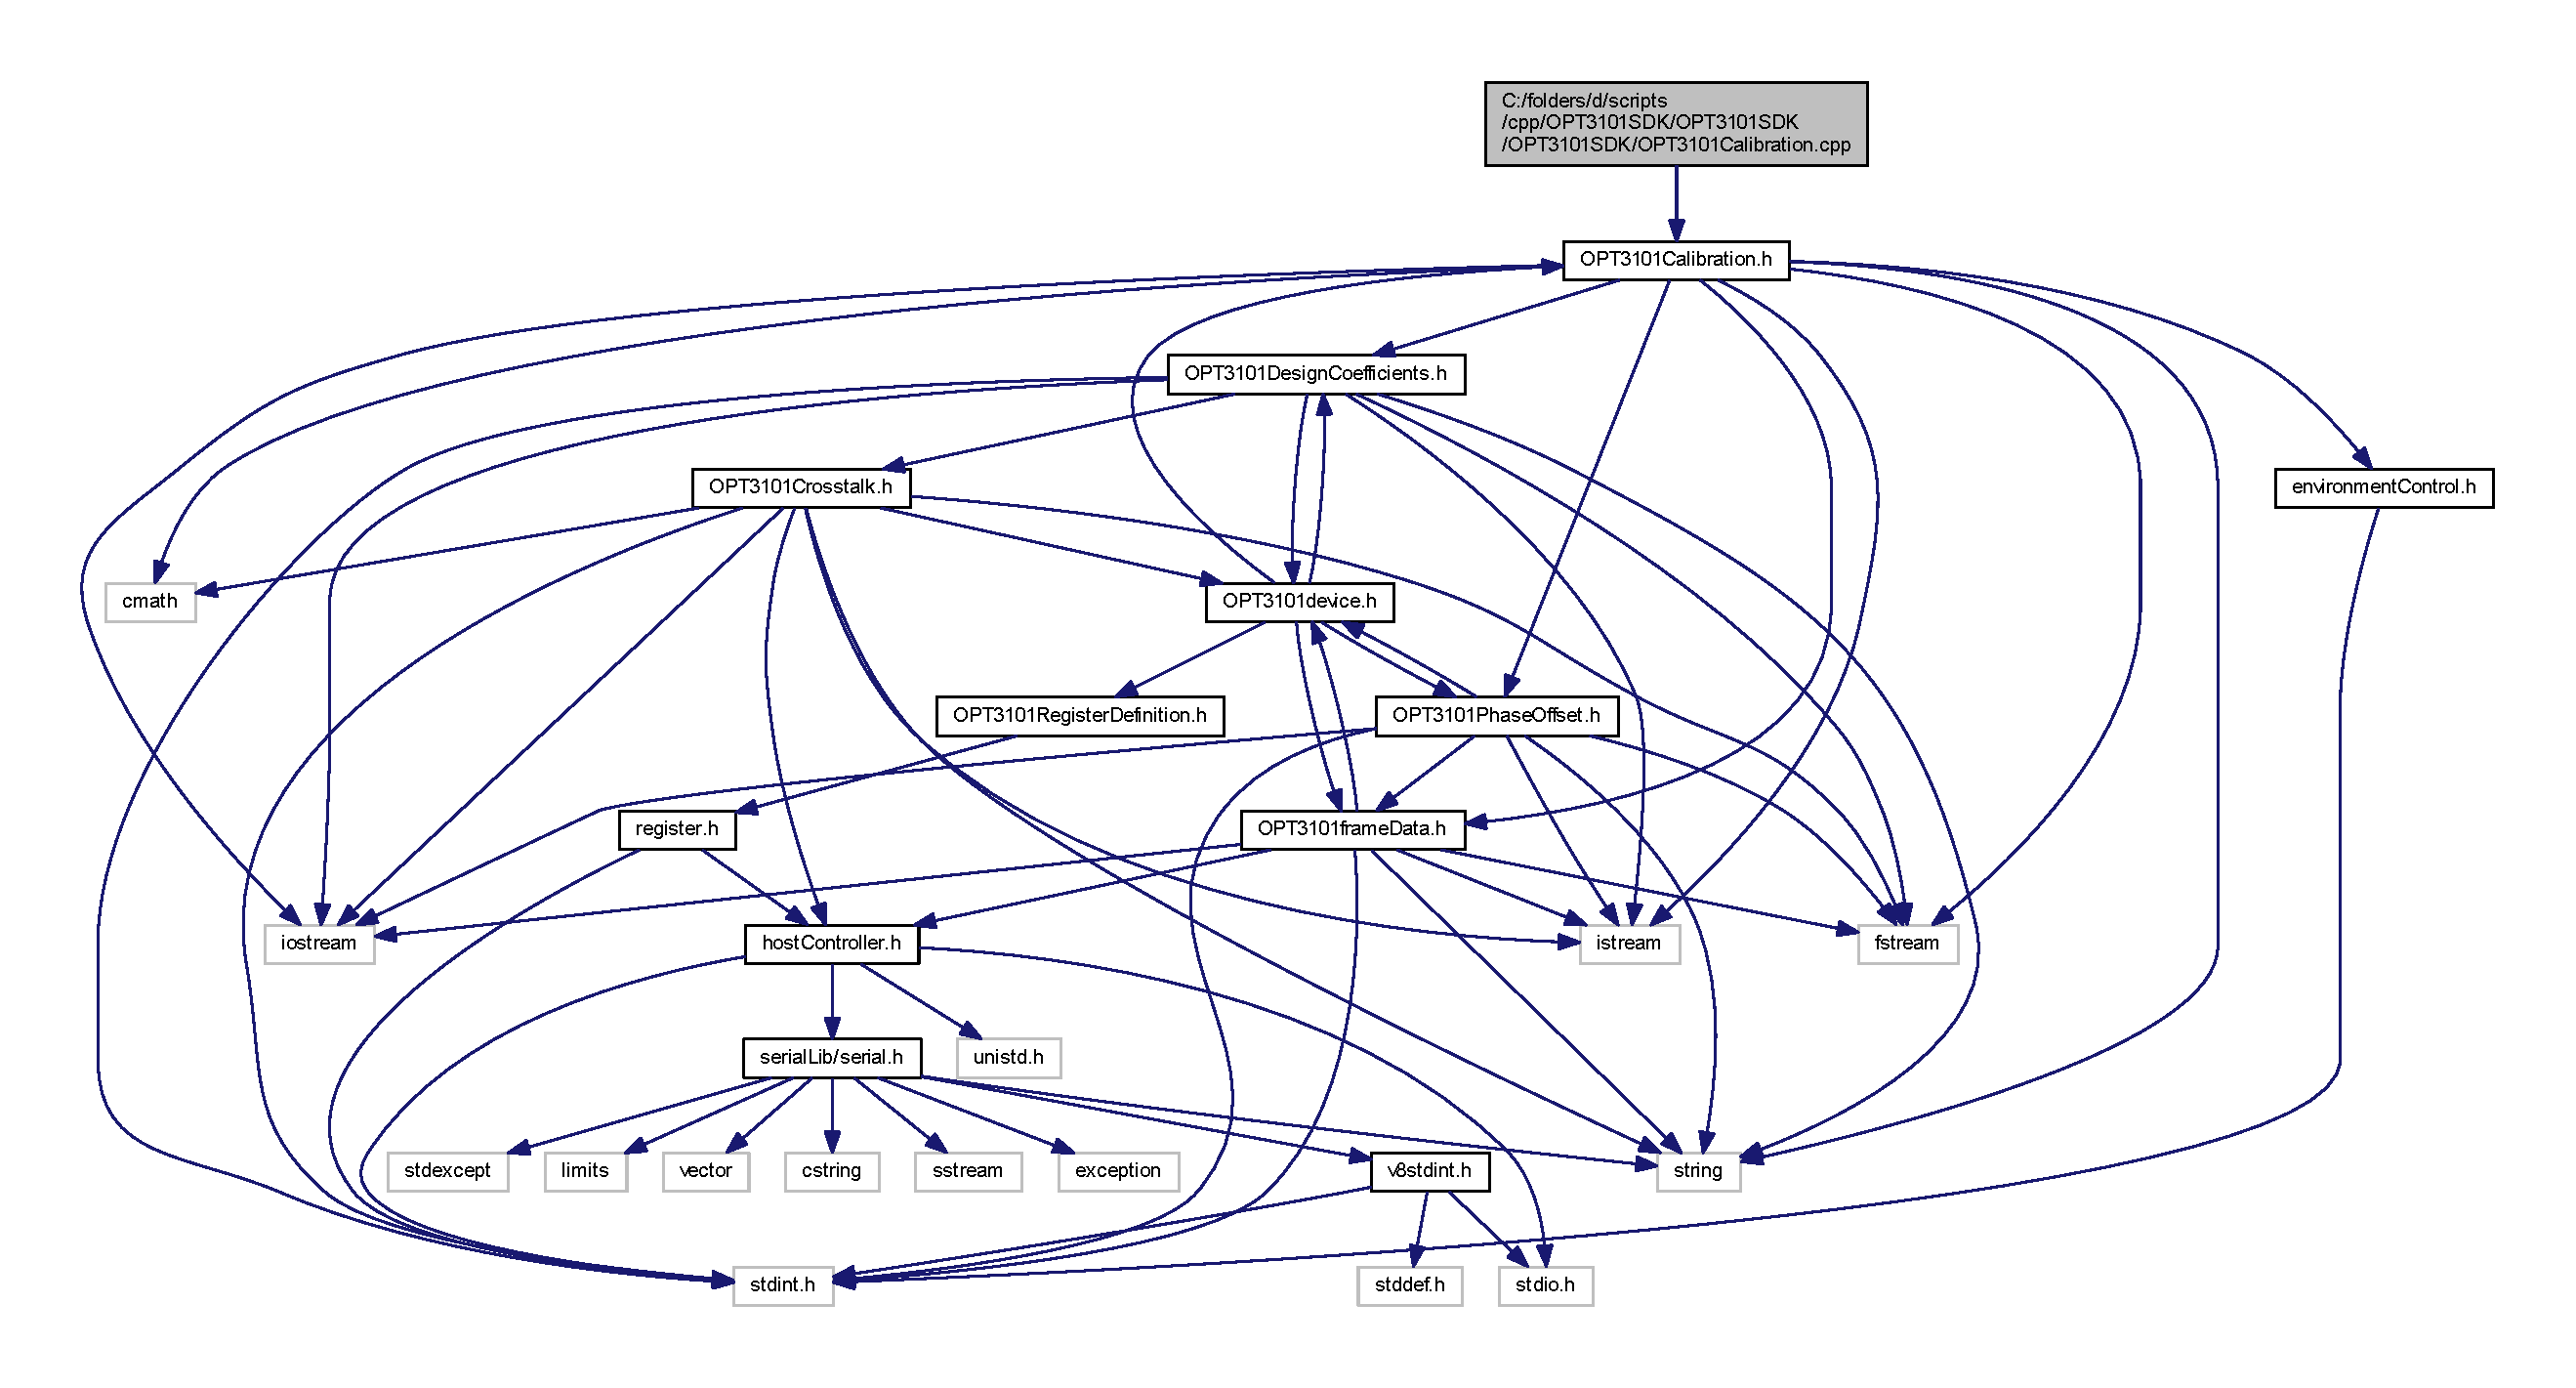
\includegraphics[width=350pt]{_o_p_t3101_calibration_8cpp__incl}
\end{center}
\end{figure}


\subsection{Detailed Description}
\begin{DoxyAuthor}{Author}
Karthik Rajagopal \href{mailto:krthik@ti.com}{\tt krthik@ti.\+com} 
\end{DoxyAuthor}
\begin{DoxyVersion}{Version}
0.\+8
\end{DoxyVersion}
\hypertarget{register_8h_COPYRIGHT}{}\subsection{C\+O\+P\+Y\+R\+I\+G\+HT}\label{register_8h_COPYRIGHT}
T\+E\+X\+AS I\+N\+S\+T\+R\+U\+M\+E\+N\+TS T\+E\+XT F\+I\+LE L\+I\+C\+E\+N\+SE Copyright (c) 2018 Texas Instruments Incorporated All rights reserved not granted herein. Limited License. Texas Instruments Incorporated grants a world-\/wide, royalty-\/free, non-\/exclusive license under copyrights and patents it now or hereafter owns or controls to make, have made, use, import, offer to sell and sell (\char`\"{}\+Utilize\char`\"{}) this software subject to the terms herein. With respect to the foregoing patent license, such license is granted solely to the extent that any such patent is necessary to Utilize the software alone. The patent license shall not apply to any combinations which include this software, other than combinations with devices manufactured by or for TI (�\+TI Devices�). No hardware patent is licensed hereunder. Redistributions must preserve existing copyright notices and reproduce this license (including the above copyright notice and the disclaimer and (if applicable) source code license limitations below) in the documentation and/or other materials provided with the distribution Redistribution and use in binary form, without modification, are permitted provided that the following conditions are met\+:
\begin{DoxyItemize}
\item No reverse engineering, decompilation, or disassembly of this software is permitted with respect to any software provided in binary form.
\item any redistribution and use are licensed by TI for use only with TI Devices.
\item Nothing shall obligate TI to provide you with source code for the software licensed and provided to you in object code. If software source code is provided to you, modification and redistribution of the source code are permitted provided that the following conditions are met\+:
\item any redistribution and use of the source code, including any resulting derivative works, are licensed by TI for use only with TI Devices.
\item any redistribution and use of any object code compiled from the source code and any resulting derivative works, are licensed by TI for use only with TI Devices. Neither the name of Texas Instruments Incorporated nor the names of its suppliers may be used to endorse or promote products derived from this software without specific prior written permission. D\+I\+S\+C\+L\+A\+I\+M\+ER. T\+H\+IS S\+O\+F\+T\+W\+A\+RE IS P\+R\+O\+V\+I\+D\+ED BY TI A\+ND T\+I�S L\+I\+C\+E\+N\+S\+O\+RS \char`\"{}\+A\+S I\+S\char`\"{} A\+ND A\+NY E\+X\+P\+R\+E\+SS OR I\+M\+P\+L\+I\+ED W\+A\+R\+R\+A\+N\+T\+I\+ES, I\+N\+C\+L\+U\+D\+I\+NG, B\+UT N\+OT L\+I\+M\+I\+T\+ED TO, T\+HE I\+M\+P\+L\+I\+ED W\+A\+R\+R\+A\+N\+T\+I\+ES OF M\+E\+R\+C\+H\+A\+N\+T\+A\+B\+I\+L\+I\+TY A\+ND F\+I\+T\+N\+E\+SS F\+OR A P\+A\+R\+T\+I\+C\+U\+L\+AR P\+U\+R\+P\+O\+SE A\+RE D\+I\+S\+C\+L\+A\+I\+M\+ED. IN NO E\+V\+E\+NT S\+H\+A\+LL TI A\+ND T\+I�S L\+I\+C\+E\+N\+S\+O\+RS BE L\+I\+A\+B\+LE F\+OR A\+NY D\+I\+R\+E\+CT, I\+N\+D\+I\+R\+E\+CT, I\+N\+C\+I\+D\+E\+N\+T\+AL, S\+P\+E\+C\+I\+AL, E\+X\+E\+M\+P\+L\+A\+RY, OR C\+O\+N\+S\+E\+Q\+U\+E\+N\+T\+I\+AL D\+A\+M\+A\+G\+ES (I\+N\+C\+L\+U\+D\+I\+NG, B\+UT N\+OT L\+I\+M\+I\+T\+ED TO, P\+R\+O\+C\+U\+R\+E\+M\+E\+NT OF S\+U\+B\+S\+T\+I\+T\+U\+TE G\+O\+O\+DS OR S\+E\+R\+V\+I\+C\+ES; L\+O\+SS OF U\+SE, D\+A\+TA, OR P\+R\+O\+F\+I\+TS; OR B\+U\+S\+I\+N\+E\+SS I\+N\+T\+E\+R\+R\+U\+P\+T\+I\+ON) H\+O\+W\+E\+V\+ER C\+A\+U\+S\+ED A\+ND ON A\+NY T\+H\+E\+O\+RY OF L\+I\+A\+B\+I\+L\+I\+TY, W\+H\+E\+T\+H\+ER IN C\+O\+N\+T\+R\+A\+CT, S\+T\+R\+I\+CT L\+I\+A\+B\+I\+L\+I\+TY, OR T\+O\+RT (I\+N\+C\+L\+U\+D\+I\+NG N\+E\+G\+L\+I\+G\+E\+N\+CE OR O\+T\+H\+E\+R\+W\+I\+SE) A\+R\+I\+S\+I\+NG IN A\+NY W\+AY O\+UT OF T\+HE U\+SE OF T\+H\+IS S\+O\+F\+T\+W\+A\+RE, E\+V\+EN IF A\+D\+V\+I\+S\+ED OF T\+HE P\+O\+S\+S\+I\+B\+I\+L\+I\+TY OF S\+U\+CH D\+A\+M\+A\+GE.
\end{DoxyItemize}\hypertarget{register_8h_DESCRIPTION}{}\subsection{D\+E\+S\+C\+R\+I\+P\+T\+I\+ON}\label{register_8h_DESCRIPTION}
This file contains the method definitions for class \mbox{\hyperlink{class_o_p_t3101_1_1calibration_c}{O\+P\+T3101\+::calibrationC}} 
\hypertarget{_o_p_t3101_calibration_8h}{}\section{C\+:/folders/d/scripts/cpp/\+O\+P\+T3101\+S\+D\+K/\+O\+P\+T3101\+S\+D\+K/\+O\+P\+T3101\+S\+D\+K/\+O\+P\+T3101\+Calibration.h File Reference}
\label{_o_p_t3101_calibration_8h}\index{C\+:/folders/d/scripts/cpp/\+O\+P\+T3101\+S\+D\+K/\+O\+P\+T3101\+S\+D\+K/\+O\+P\+T3101\+S\+D\+K/\+O\+P\+T3101\+Calibration.\+h@{C\+:/folders/d/scripts/cpp/\+O\+P\+T3101\+S\+D\+K/\+O\+P\+T3101\+S\+D\+K/\+O\+P\+T3101\+S\+D\+K/\+O\+P\+T3101\+Calibration.\+h}}
{\ttfamily \#include $<$cmath$>$}\newline
{\ttfamily \#include \char`\"{}O\+P\+T3101\+Design\+Coefficients.\+h\char`\"{}}\newline
{\ttfamily \#include \char`\"{}O\+P\+T3101frame\+Data.\+h\char`\"{}}\newline
{\ttfamily \#include \char`\"{}O\+P\+T3101\+Phase\+Offset.\+h\char`\"{}}\newline
{\ttfamily \#include \char`\"{}environment\+Control.\+h\char`\"{}}\newline
{\ttfamily \#include $<$fstream$>$}\newline
{\ttfamily \#include $<$iostream$>$}\newline
{\ttfamily \#include $<$istream$>$}\newline
{\ttfamily \#include $<$string$>$}\newline
Include dependency graph for O\+P\+T3101\+Calibration.\+h\+:\nopagebreak
\begin{figure}[H]
\begin{center}
\leavevmode
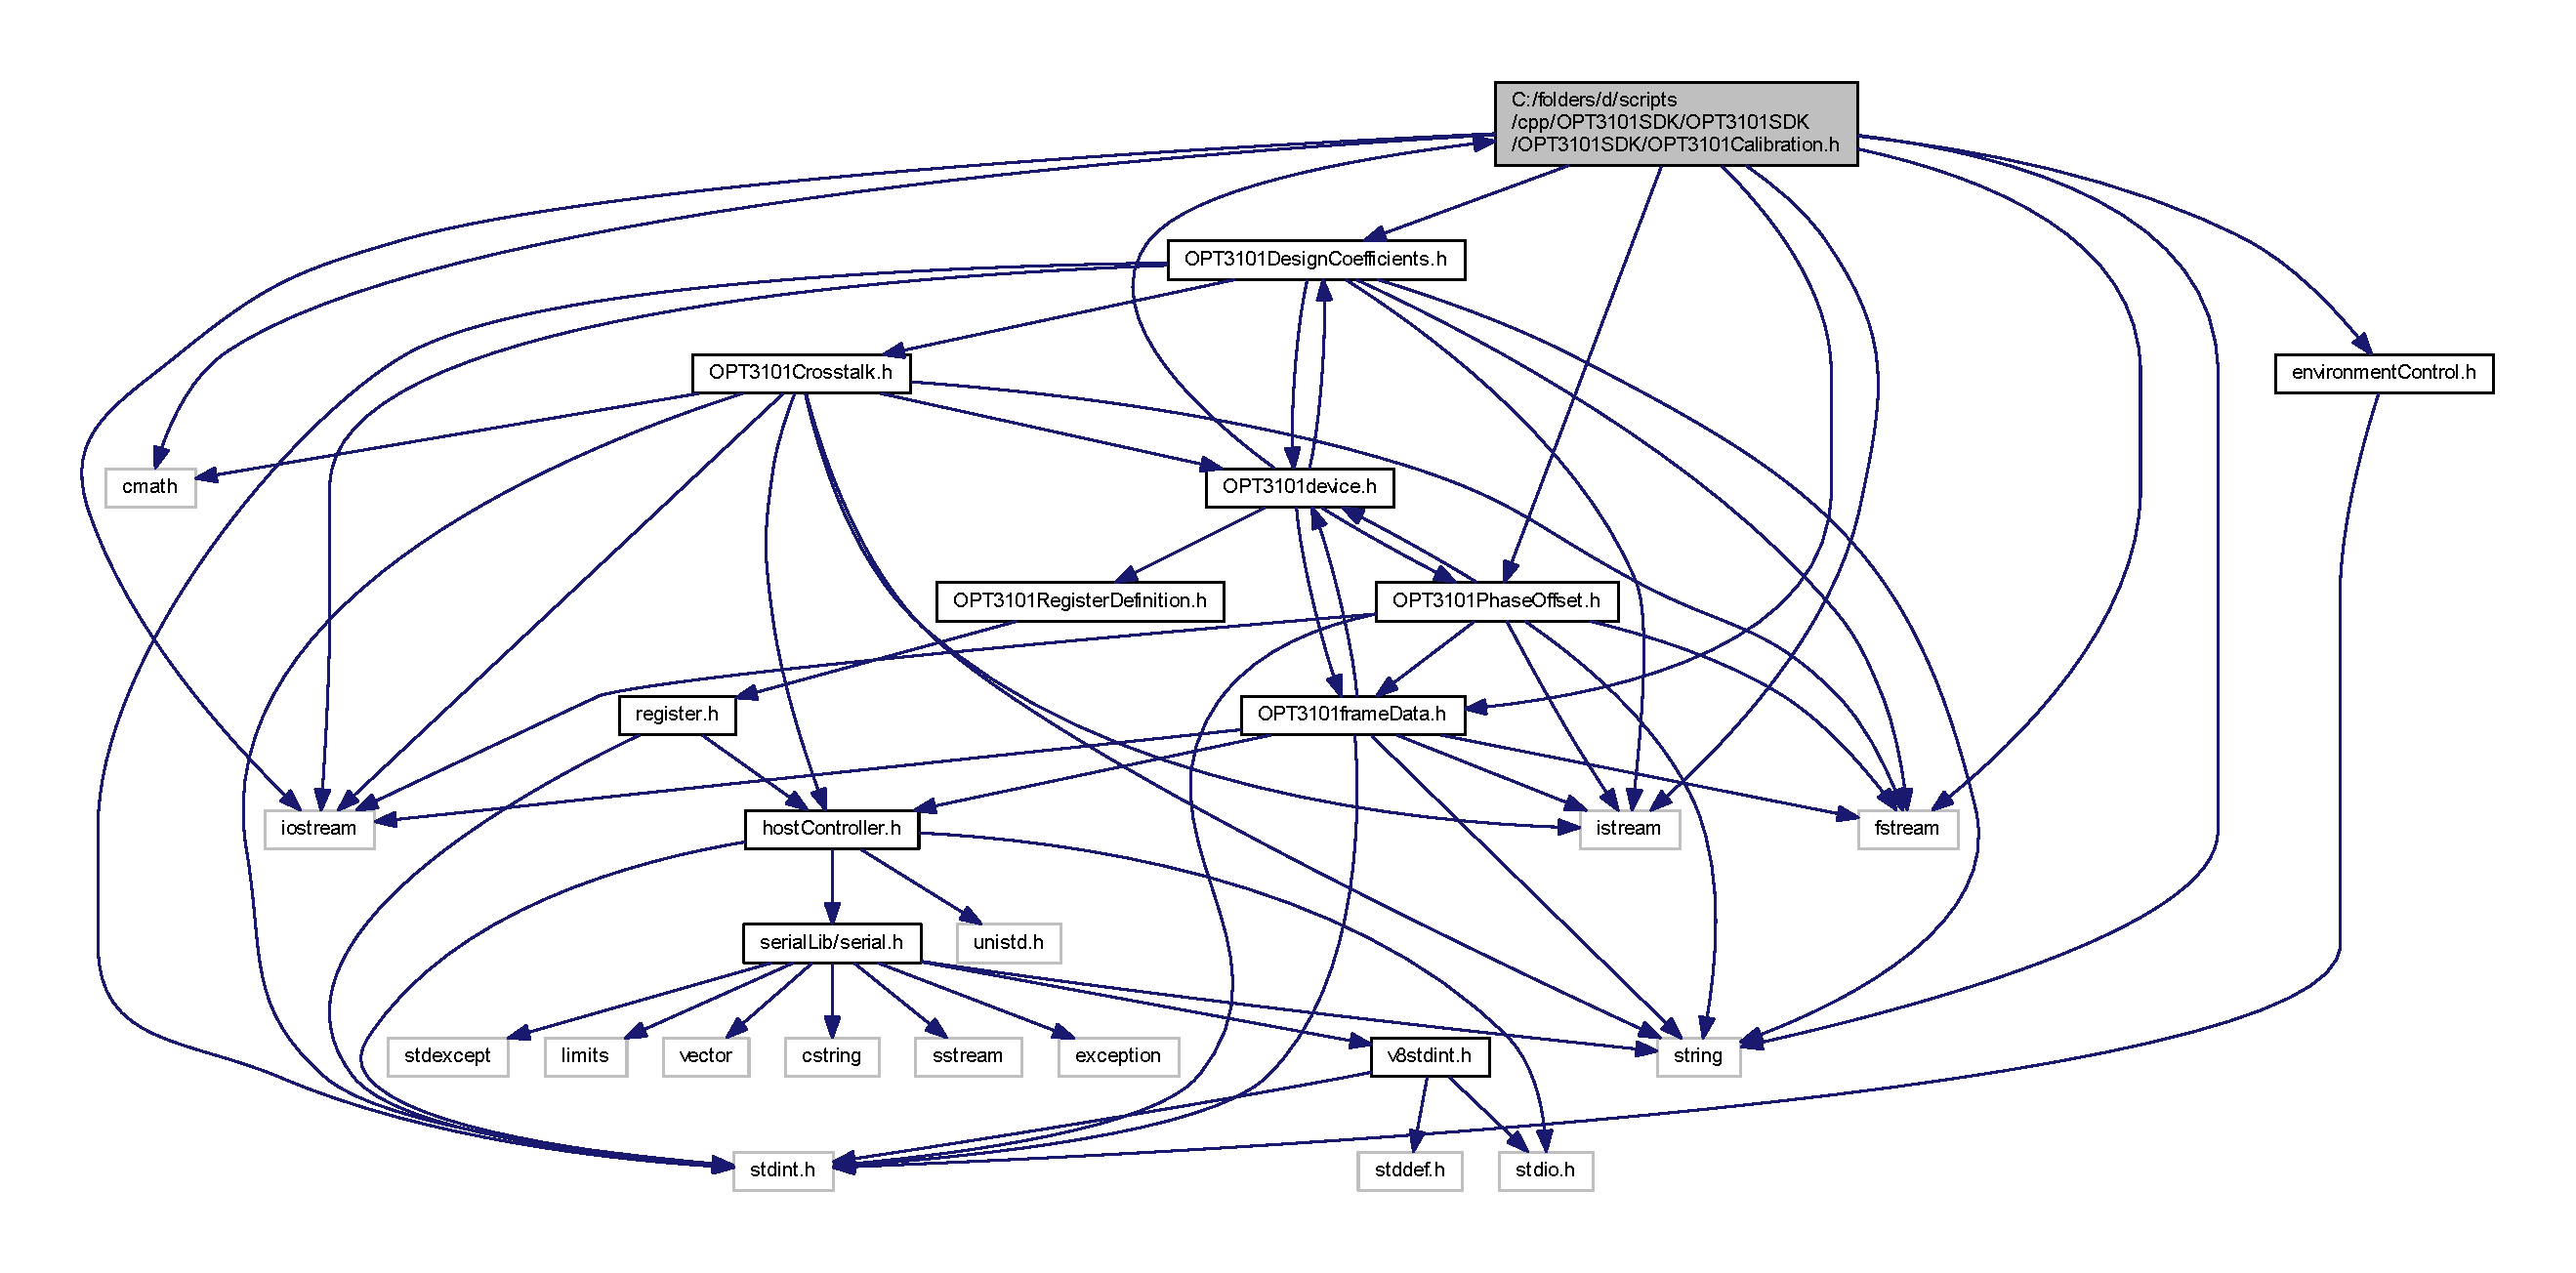
\includegraphics[width=350pt]{_o_p_t3101_calibration_8h__incl}
\end{center}
\end{figure}
This graph shows which files directly or indirectly include this file\+:\nopagebreak
\begin{figure}[H]
\begin{center}
\leavevmode
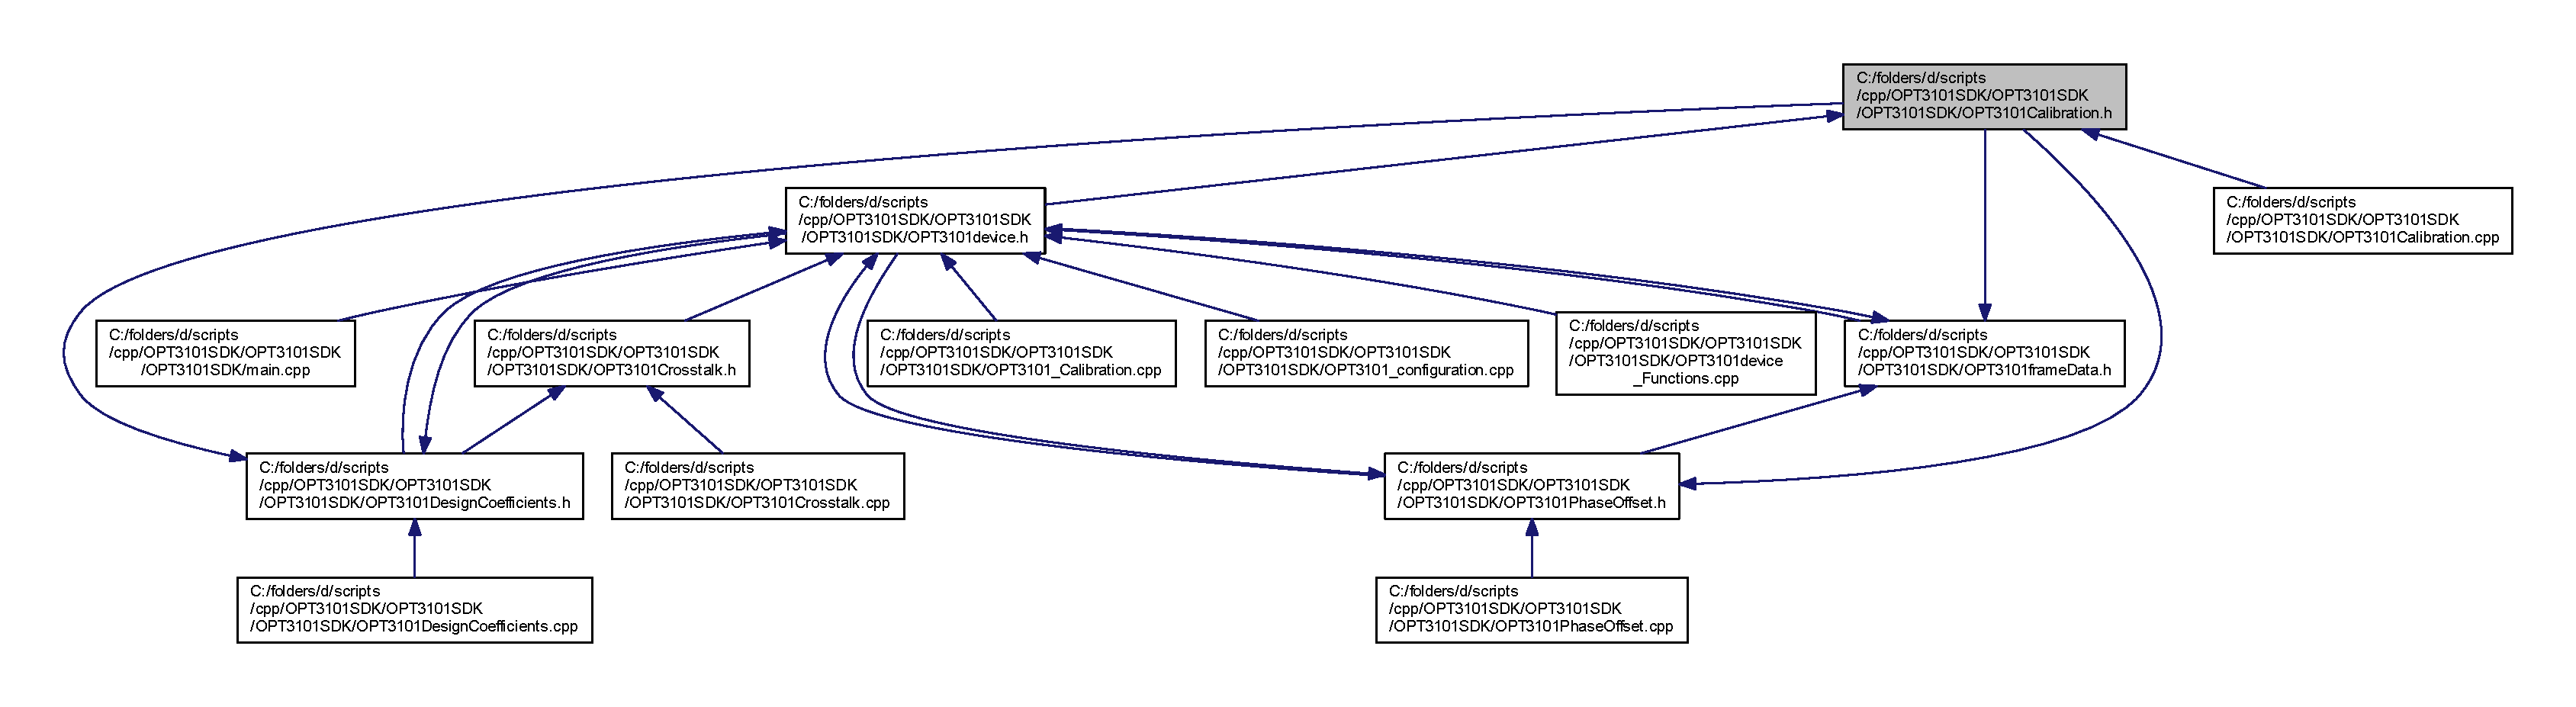
\includegraphics[width=350pt]{_o_p_t3101_calibration_8h__dep__incl}
\end{center}
\end{figure}
\subsection*{Classes}
\begin{DoxyCompactItemize}
\item 
class \mbox{\hyperlink{class_o_p_t3101_1_1calibration_c}{O\+P\+T3101\+::calibrationC}}
\begin{DoxyCompactList}\small\item\em Class contains the instances of classes required during \mbox{\hyperlink{namespace_o_p_t3101}{O\+P\+T3101}} calibration. \end{DoxyCompactList}\end{DoxyCompactItemize}
\subsection*{Namespaces}
\begin{DoxyCompactItemize}
\item 
 \mbox{\hyperlink{namespace_o_p_t3101}{O\+P\+T3101}}
\begin{DoxyCompactList}\small\item\em \mbox{\hyperlink{class_o_p_t3101_1_1device}{O\+P\+T3101\+::device}} declaration This is declared here to avoid cyclic reference of classes. \end{DoxyCompactList}\end{DoxyCompactItemize}
\subsection*{Variables}
\begin{DoxyCompactItemize}
\item 
\mbox{\hyperlink{classenvironmental_controller}{environmental\+Controller}} \mbox{\hyperlink{_o_p_t3101_calibration_8h_abf2c91dbdc70c87e1f27292a948c77ab}{env\+Controller}}
\begin{DoxyCompactList}\small\item\em \mbox{\hyperlink{classenvironmental_controller}{environmental\+Controller}} class instance declaration This global variable declaration to be available across files which controls the environmental parameters. The instance is of class \mbox{\hyperlink{classenvironmental_controller}{environmental\+Controller}} \end{DoxyCompactList}\end{DoxyCompactItemize}


\subsection{Detailed Description}
\begin{DoxyAuthor}{Author}
Karthik Rajagopal \href{mailto:krthik@ti.com}{\tt krthik@ti.\+com} 
\end{DoxyAuthor}
\begin{DoxyVersion}{Version}
0.\+8
\end{DoxyVersion}
\hypertarget{register_8h_COPYRIGHT}{}\subsection{C\+O\+P\+Y\+R\+I\+G\+HT}\label{register_8h_COPYRIGHT}
T\+E\+X\+AS I\+N\+S\+T\+R\+U\+M\+E\+N\+TS T\+E\+XT F\+I\+LE L\+I\+C\+E\+N\+SE Copyright (c) 2018 Texas Instruments Incorporated All rights reserved not granted herein. Limited License. Texas Instruments Incorporated grants a world-\/wide, royalty-\/free, non-\/exclusive license under copyrights and patents it now or hereafter owns or controls to make, have made, use, import, offer to sell and sell (\char`\"{}\+Utilize\char`\"{}) this software subject to the terms herein. With respect to the foregoing patent license, such license is granted solely to the extent that any such patent is necessary to Utilize the software alone. The patent license shall not apply to any combinations which include this software, other than combinations with devices manufactured by or for TI (�\+TI Devices�). No hardware patent is licensed hereunder. Redistributions must preserve existing copyright notices and reproduce this license (including the above copyright notice and the disclaimer and (if applicable) source code license limitations below) in the documentation and/or other materials provided with the distribution Redistribution and use in binary form, without modification, are permitted provided that the following conditions are met\+:
\begin{DoxyItemize}
\item No reverse engineering, decompilation, or disassembly of this software is permitted with respect to any software provided in binary form.
\item any redistribution and use are licensed by TI for use only with TI Devices.
\item Nothing shall obligate TI to provide you with source code for the software licensed and provided to you in object code. If software source code is provided to you, modification and redistribution of the source code are permitted provided that the following conditions are met\+:
\item any redistribution and use of the source code, including any resulting derivative works, are licensed by TI for use only with TI Devices.
\item any redistribution and use of any object code compiled from the source code and any resulting derivative works, are licensed by TI for use only with TI Devices. Neither the name of Texas Instruments Incorporated nor the names of its suppliers may be used to endorse or promote products derived from this software without specific prior written permission. D\+I\+S\+C\+L\+A\+I\+M\+ER. T\+H\+IS S\+O\+F\+T\+W\+A\+RE IS P\+R\+O\+V\+I\+D\+ED BY TI A\+ND T\+I�S L\+I\+C\+E\+N\+S\+O\+RS \char`\"{}\+A\+S I\+S\char`\"{} A\+ND A\+NY E\+X\+P\+R\+E\+SS OR I\+M\+P\+L\+I\+ED W\+A\+R\+R\+A\+N\+T\+I\+ES, I\+N\+C\+L\+U\+D\+I\+NG, B\+UT N\+OT L\+I\+M\+I\+T\+ED TO, T\+HE I\+M\+P\+L\+I\+ED W\+A\+R\+R\+A\+N\+T\+I\+ES OF M\+E\+R\+C\+H\+A\+N\+T\+A\+B\+I\+L\+I\+TY A\+ND F\+I\+T\+N\+E\+SS F\+OR A P\+A\+R\+T\+I\+C\+U\+L\+AR P\+U\+R\+P\+O\+SE A\+RE D\+I\+S\+C\+L\+A\+I\+M\+ED. IN NO E\+V\+E\+NT S\+H\+A\+LL TI A\+ND T\+I�S L\+I\+C\+E\+N\+S\+O\+RS BE L\+I\+A\+B\+LE F\+OR A\+NY D\+I\+R\+E\+CT, I\+N\+D\+I\+R\+E\+CT, I\+N\+C\+I\+D\+E\+N\+T\+AL, S\+P\+E\+C\+I\+AL, E\+X\+E\+M\+P\+L\+A\+RY, OR C\+O\+N\+S\+E\+Q\+U\+E\+N\+T\+I\+AL D\+A\+M\+A\+G\+ES (I\+N\+C\+L\+U\+D\+I\+NG, B\+UT N\+OT L\+I\+M\+I\+T\+ED TO, P\+R\+O\+C\+U\+R\+E\+M\+E\+NT OF S\+U\+B\+S\+T\+I\+T\+U\+TE G\+O\+O\+DS OR S\+E\+R\+V\+I\+C\+ES; L\+O\+SS OF U\+SE, D\+A\+TA, OR P\+R\+O\+F\+I\+TS; OR B\+U\+S\+I\+N\+E\+SS I\+N\+T\+E\+R\+R\+U\+P\+T\+I\+ON) H\+O\+W\+E\+V\+ER C\+A\+U\+S\+ED A\+ND ON A\+NY T\+H\+E\+O\+RY OF L\+I\+A\+B\+I\+L\+I\+TY, W\+H\+E\+T\+H\+ER IN C\+O\+N\+T\+R\+A\+CT, S\+T\+R\+I\+CT L\+I\+A\+B\+I\+L\+I\+TY, OR T\+O\+RT (I\+N\+C\+L\+U\+D\+I\+NG N\+E\+G\+L\+I\+G\+E\+N\+CE OR O\+T\+H\+E\+R\+W\+I\+SE) A\+R\+I\+S\+I\+NG IN A\+NY W\+AY O\+UT OF T\+HE U\+SE OF T\+H\+IS S\+O\+F\+T\+W\+A\+RE, E\+V\+EN IF A\+D\+V\+I\+S\+ED OF T\+HE P\+O\+S\+S\+I\+B\+I\+L\+I\+TY OF S\+U\+CH D\+A\+M\+A\+GE.
\end{DoxyItemize}\hypertarget{register_8h_DESCRIPTION}{}\subsection{D\+E\+S\+C\+R\+I\+P\+T\+I\+ON}\label{register_8h_DESCRIPTION}
This file contains the \mbox{\hyperlink{class_o_p_t3101_1_1calibration_c}{O\+P\+T3101\+::calibrationC}} class declaration 

\subsection{Variable Documentation}
\mbox{\Hypertarget{_o_p_t3101_calibration_8h_abf2c91dbdc70c87e1f27292a948c77ab}\label{_o_p_t3101_calibration_8h_abf2c91dbdc70c87e1f27292a948c77ab}} 
\index{O\+P\+T3101\+Calibration.\+h@{O\+P\+T3101\+Calibration.\+h}!env\+Controller@{env\+Controller}}
\index{env\+Controller@{env\+Controller}!O\+P\+T3101\+Calibration.\+h@{O\+P\+T3101\+Calibration.\+h}}
\subsubsection{\texorpdfstring{env\+Controller}{envController}}
{\footnotesize\ttfamily \mbox{\hyperlink{classenvironmental_controller}{environmental\+Controller}} env\+Controller}



\mbox{\hyperlink{classenvironmental_controller}{environmental\+Controller}} class instance declaration This global variable declaration to be available across files which controls the environmental parameters. The instance is of class \mbox{\hyperlink{classenvironmental_controller}{environmental\+Controller}} 

\mbox{\hyperlink{classenvironmental_controller}{environmental\+Controller}} class instance declaration This global variable declaration to be available across files which controls the environmental parameters. The instance is of class \mbox{\hyperlink{classenvironmental_controller}{environmental\+Controller}} 
\hypertarget{_o_p_t3101_crosstalk_8cpp}{}\section{C\+:/folders/d/scripts/cpp/\+O\+P\+T3101\+S\+D\+K/\+O\+P\+T3101\+S\+D\+K/\+O\+P\+T3101\+S\+D\+K/\+O\+P\+T3101\+Crosstalk.cpp File Reference}
\label{_o_p_t3101_crosstalk_8cpp}\index{C\+:/folders/d/scripts/cpp/\+O\+P\+T3101\+S\+D\+K/\+O\+P\+T3101\+S\+D\+K/\+O\+P\+T3101\+S\+D\+K/\+O\+P\+T3101\+Crosstalk.\+cpp@{C\+:/folders/d/scripts/cpp/\+O\+P\+T3101\+S\+D\+K/\+O\+P\+T3101\+S\+D\+K/\+O\+P\+T3101\+S\+D\+K/\+O\+P\+T3101\+Crosstalk.\+cpp}}
{\ttfamily \#include \char`\"{}O\+P\+T3101\+Crosstalk.\+h\char`\"{}}\newline
{\ttfamily \#include \char`\"{}host\+Controller.\+h\char`\"{}}\newline
Include dependency graph for O\+P\+T3101\+Crosstalk.\+cpp\+:\nopagebreak
\begin{figure}[H]
\begin{center}
\leavevmode
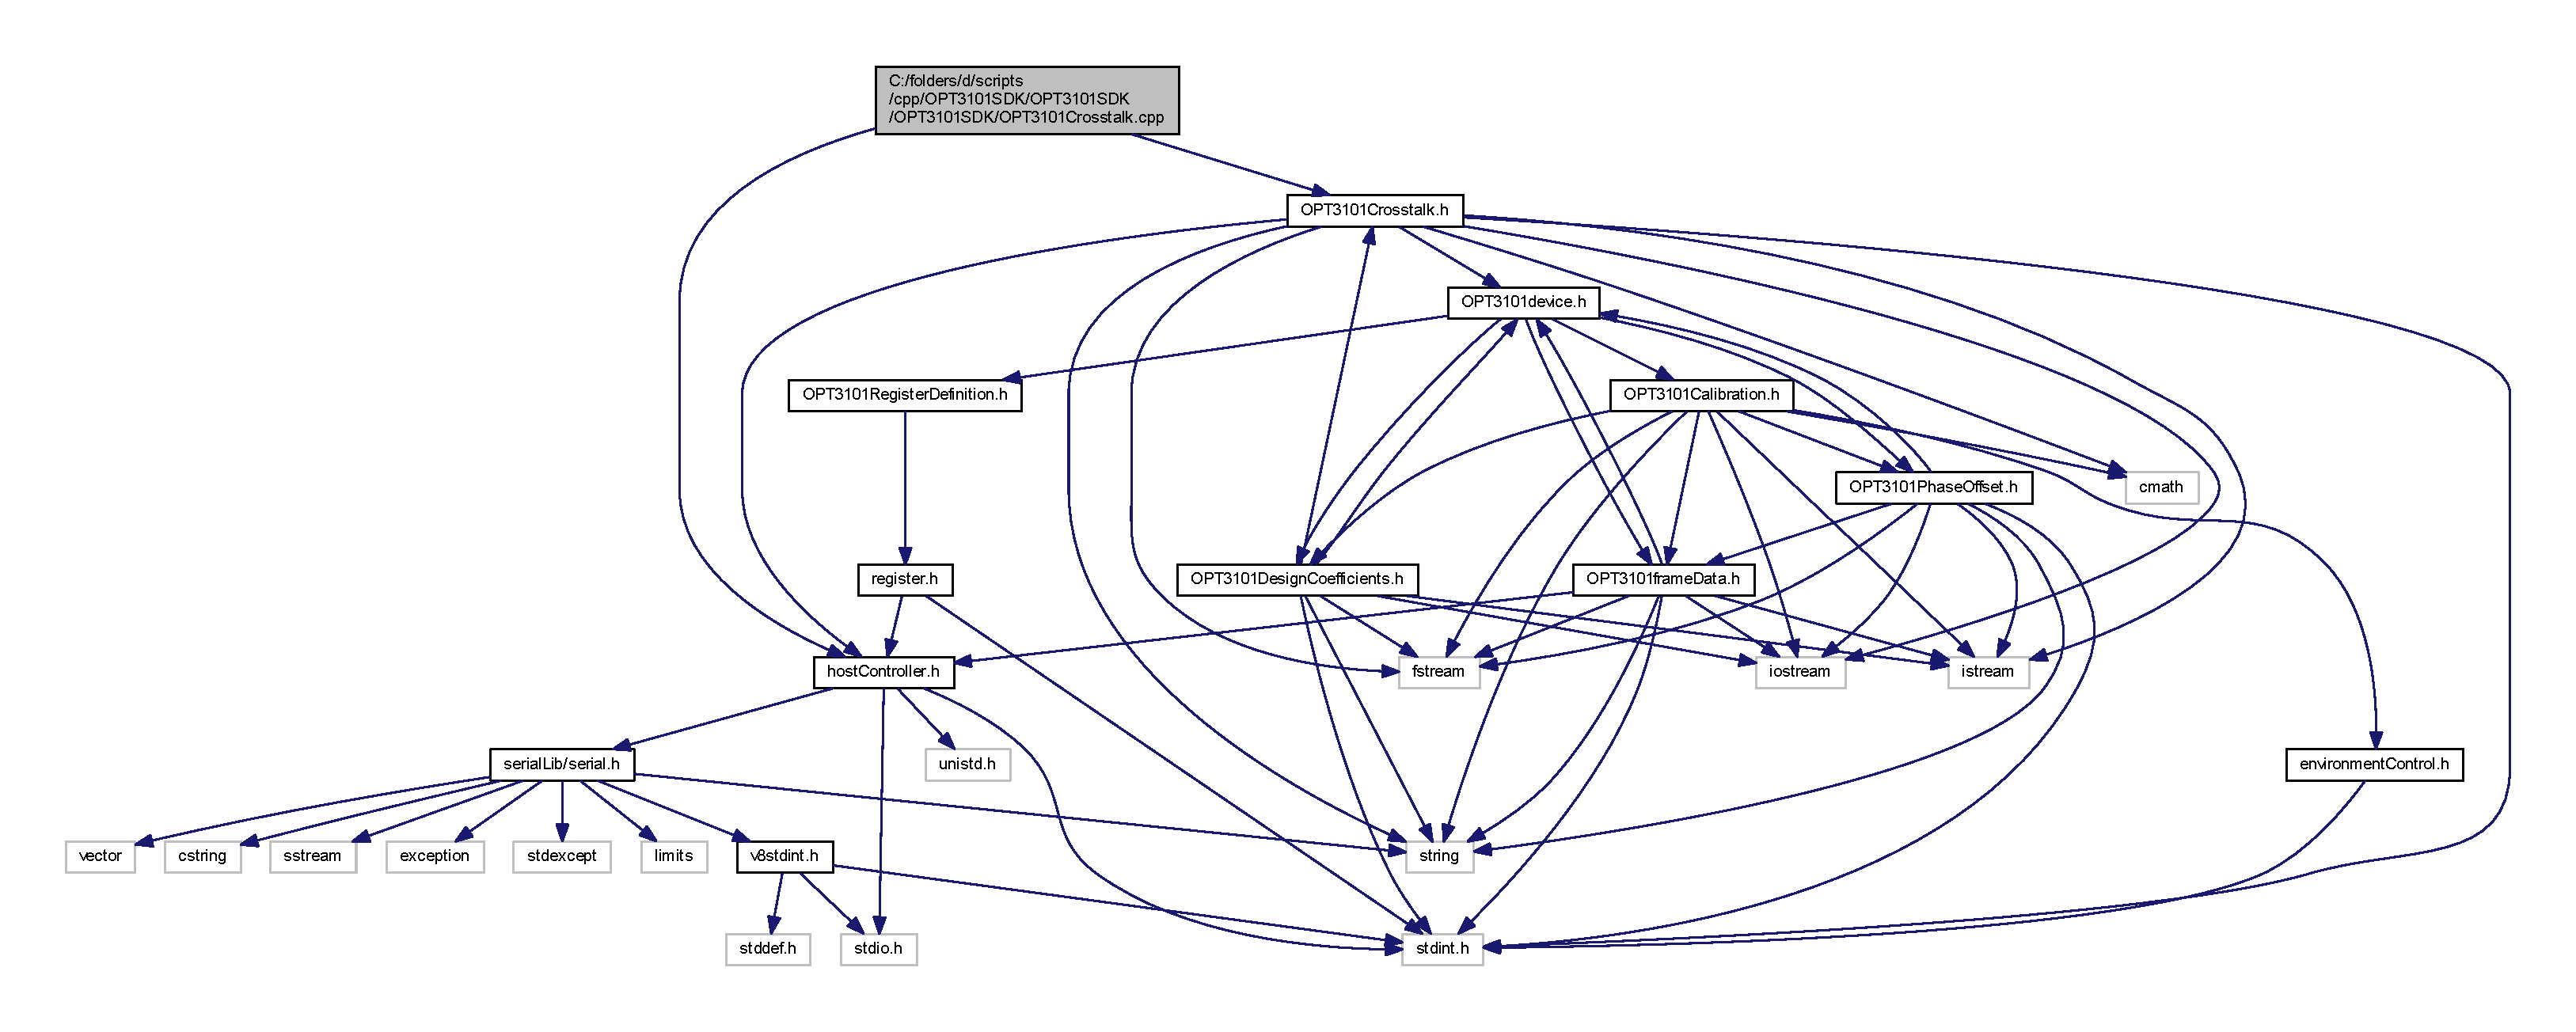
\includegraphics[width=350pt]{_o_p_t3101_crosstalk_8cpp__incl}
\end{center}
\end{figure}


\subsection{Detailed Description}
\begin{DoxyAuthor}{Author}
Karthik Rajagopal \href{mailto:krthik@ti.com}{\tt krthik@ti.\+com} 
\end{DoxyAuthor}
\begin{DoxyVersion}{Version}
0.\+8
\end{DoxyVersion}
\hypertarget{register_8h_COPYRIGHT}{}\subsection{C\+O\+P\+Y\+R\+I\+G\+HT}\label{register_8h_COPYRIGHT}
T\+E\+X\+AS I\+N\+S\+T\+R\+U\+M\+E\+N\+TS T\+E\+XT F\+I\+LE L\+I\+C\+E\+N\+SE Copyright (c) 2018 Texas Instruments Incorporated All rights reserved not granted herein. Limited License. Texas Instruments Incorporated grants a world-\/wide, royalty-\/free, non-\/exclusive license under copyrights and patents it now or hereafter owns or controls to make, have made, use, import, offer to sell and sell (\char`\"{}\+Utilize\char`\"{}) this software subject to the terms herein. With respect to the foregoing patent license, such license is granted solely to the extent that any such patent is necessary to Utilize the software alone. The patent license shall not apply to any combinations which include this software, other than combinations with devices manufactured by or for TI (�\+TI Devices�). No hardware patent is licensed hereunder. Redistributions must preserve existing copyright notices and reproduce this license (including the above copyright notice and the disclaimer and (if applicable) source code license limitations below) in the documentation and/or other materials provided with the distribution Redistribution and use in binary form, without modification, are permitted provided that the following conditions are met\+:
\begin{DoxyItemize}
\item No reverse engineering, decompilation, or disassembly of this software is permitted with respect to any software provided in binary form.
\item any redistribution and use are licensed by TI for use only with TI Devices.
\item Nothing shall obligate TI to provide you with source code for the software licensed and provided to you in object code. If software source code is provided to you, modification and redistribution of the source code are permitted provided that the following conditions are met\+:
\item any redistribution and use of the source code, including any resulting derivative works, are licensed by TI for use only with TI Devices.
\item any redistribution and use of any object code compiled from the source code and any resulting derivative works, are licensed by TI for use only with TI Devices. Neither the name of Texas Instruments Incorporated nor the names of its suppliers may be used to endorse or promote products derived from this software without specific prior written permission. D\+I\+S\+C\+L\+A\+I\+M\+ER. T\+H\+IS S\+O\+F\+T\+W\+A\+RE IS P\+R\+O\+V\+I\+D\+ED BY TI A\+ND T\+I�S L\+I\+C\+E\+N\+S\+O\+RS \char`\"{}\+A\+S I\+S\char`\"{} A\+ND A\+NY E\+X\+P\+R\+E\+SS OR I\+M\+P\+L\+I\+ED W\+A\+R\+R\+A\+N\+T\+I\+ES, I\+N\+C\+L\+U\+D\+I\+NG, B\+UT N\+OT L\+I\+M\+I\+T\+ED TO, T\+HE I\+M\+P\+L\+I\+ED W\+A\+R\+R\+A\+N\+T\+I\+ES OF M\+E\+R\+C\+H\+A\+N\+T\+A\+B\+I\+L\+I\+TY A\+ND F\+I\+T\+N\+E\+SS F\+OR A P\+A\+R\+T\+I\+C\+U\+L\+AR P\+U\+R\+P\+O\+SE A\+RE D\+I\+S\+C\+L\+A\+I\+M\+ED. IN NO E\+V\+E\+NT S\+H\+A\+LL TI A\+ND T\+I�S L\+I\+C\+E\+N\+S\+O\+RS BE L\+I\+A\+B\+LE F\+OR A\+NY D\+I\+R\+E\+CT, I\+N\+D\+I\+R\+E\+CT, I\+N\+C\+I\+D\+E\+N\+T\+AL, S\+P\+E\+C\+I\+AL, E\+X\+E\+M\+P\+L\+A\+RY, OR C\+O\+N\+S\+E\+Q\+U\+E\+N\+T\+I\+AL D\+A\+M\+A\+G\+ES (I\+N\+C\+L\+U\+D\+I\+NG, B\+UT N\+OT L\+I\+M\+I\+T\+ED TO, P\+R\+O\+C\+U\+R\+E\+M\+E\+NT OF S\+U\+B\+S\+T\+I\+T\+U\+TE G\+O\+O\+DS OR S\+E\+R\+V\+I\+C\+ES; L\+O\+SS OF U\+SE, D\+A\+TA, OR P\+R\+O\+F\+I\+TS; OR B\+U\+S\+I\+N\+E\+SS I\+N\+T\+E\+R\+R\+U\+P\+T\+I\+ON) H\+O\+W\+E\+V\+ER C\+A\+U\+S\+ED A\+ND ON A\+NY T\+H\+E\+O\+RY OF L\+I\+A\+B\+I\+L\+I\+TY, W\+H\+E\+T\+H\+ER IN C\+O\+N\+T\+R\+A\+CT, S\+T\+R\+I\+CT L\+I\+A\+B\+I\+L\+I\+TY, OR T\+O\+RT (I\+N\+C\+L\+U\+D\+I\+NG N\+E\+G\+L\+I\+G\+E\+N\+CE OR O\+T\+H\+E\+R\+W\+I\+SE) A\+R\+I\+S\+I\+NG IN A\+NY W\+AY O\+UT OF T\+HE U\+SE OF T\+H\+IS S\+O\+F\+T\+W\+A\+RE, E\+V\+EN IF A\+D\+V\+I\+S\+ED OF T\+HE P\+O\+S\+S\+I\+B\+I\+L\+I\+TY OF S\+U\+CH D\+A\+M\+A\+GE.
\end{DoxyItemize}\hypertarget{register_8h_DESCRIPTION}{}\subsection{D\+E\+S\+C\+R\+I\+P\+T\+I\+ON}\label{register_8h_DESCRIPTION}
The file contains class \mbox{\hyperlink{class_o_p_t3101_1_1crosstalk_c}{O\+P\+T3101\+::crosstalkC}} member function definitions 
\hypertarget{_o_p_t3101_crosstalk_8h}{}\section{C\+:/folders/d/scripts/cpp/\+O\+P\+T3101\+S\+D\+K/\+O\+P\+T3101\+S\+D\+K/\+O\+P\+T3101\+S\+D\+K/\+O\+P\+T3101\+Crosstalk.h File Reference}
\label{_o_p_t3101_crosstalk_8h}\index{C\+:/folders/d/scripts/cpp/\+O\+P\+T3101\+S\+D\+K/\+O\+P\+T3101\+S\+D\+K/\+O\+P\+T3101\+S\+D\+K/\+O\+P\+T3101\+Crosstalk.\+h@{C\+:/folders/d/scripts/cpp/\+O\+P\+T3101\+S\+D\+K/\+O\+P\+T3101\+S\+D\+K/\+O\+P\+T3101\+S\+D\+K/\+O\+P\+T3101\+Crosstalk.\+h}}
{\ttfamily \#include $<$stdint.\+h$>$}\newline
{\ttfamily \#include $<$cmath$>$}\newline
{\ttfamily \#include \char`\"{}O\+P\+T3101device.\+h\char`\"{}}\newline
{\ttfamily \#include \char`\"{}host\+Controller.\+h\char`\"{}}\newline
{\ttfamily \#include $<$fstream$>$}\newline
{\ttfamily \#include $<$iostream$>$}\newline
{\ttfamily \#include $<$istream$>$}\newline
{\ttfamily \#include $<$string$>$}\newline
Include dependency graph for O\+P\+T3101\+Crosstalk.\+h\+:\nopagebreak
\begin{figure}[H]
\begin{center}
\leavevmode
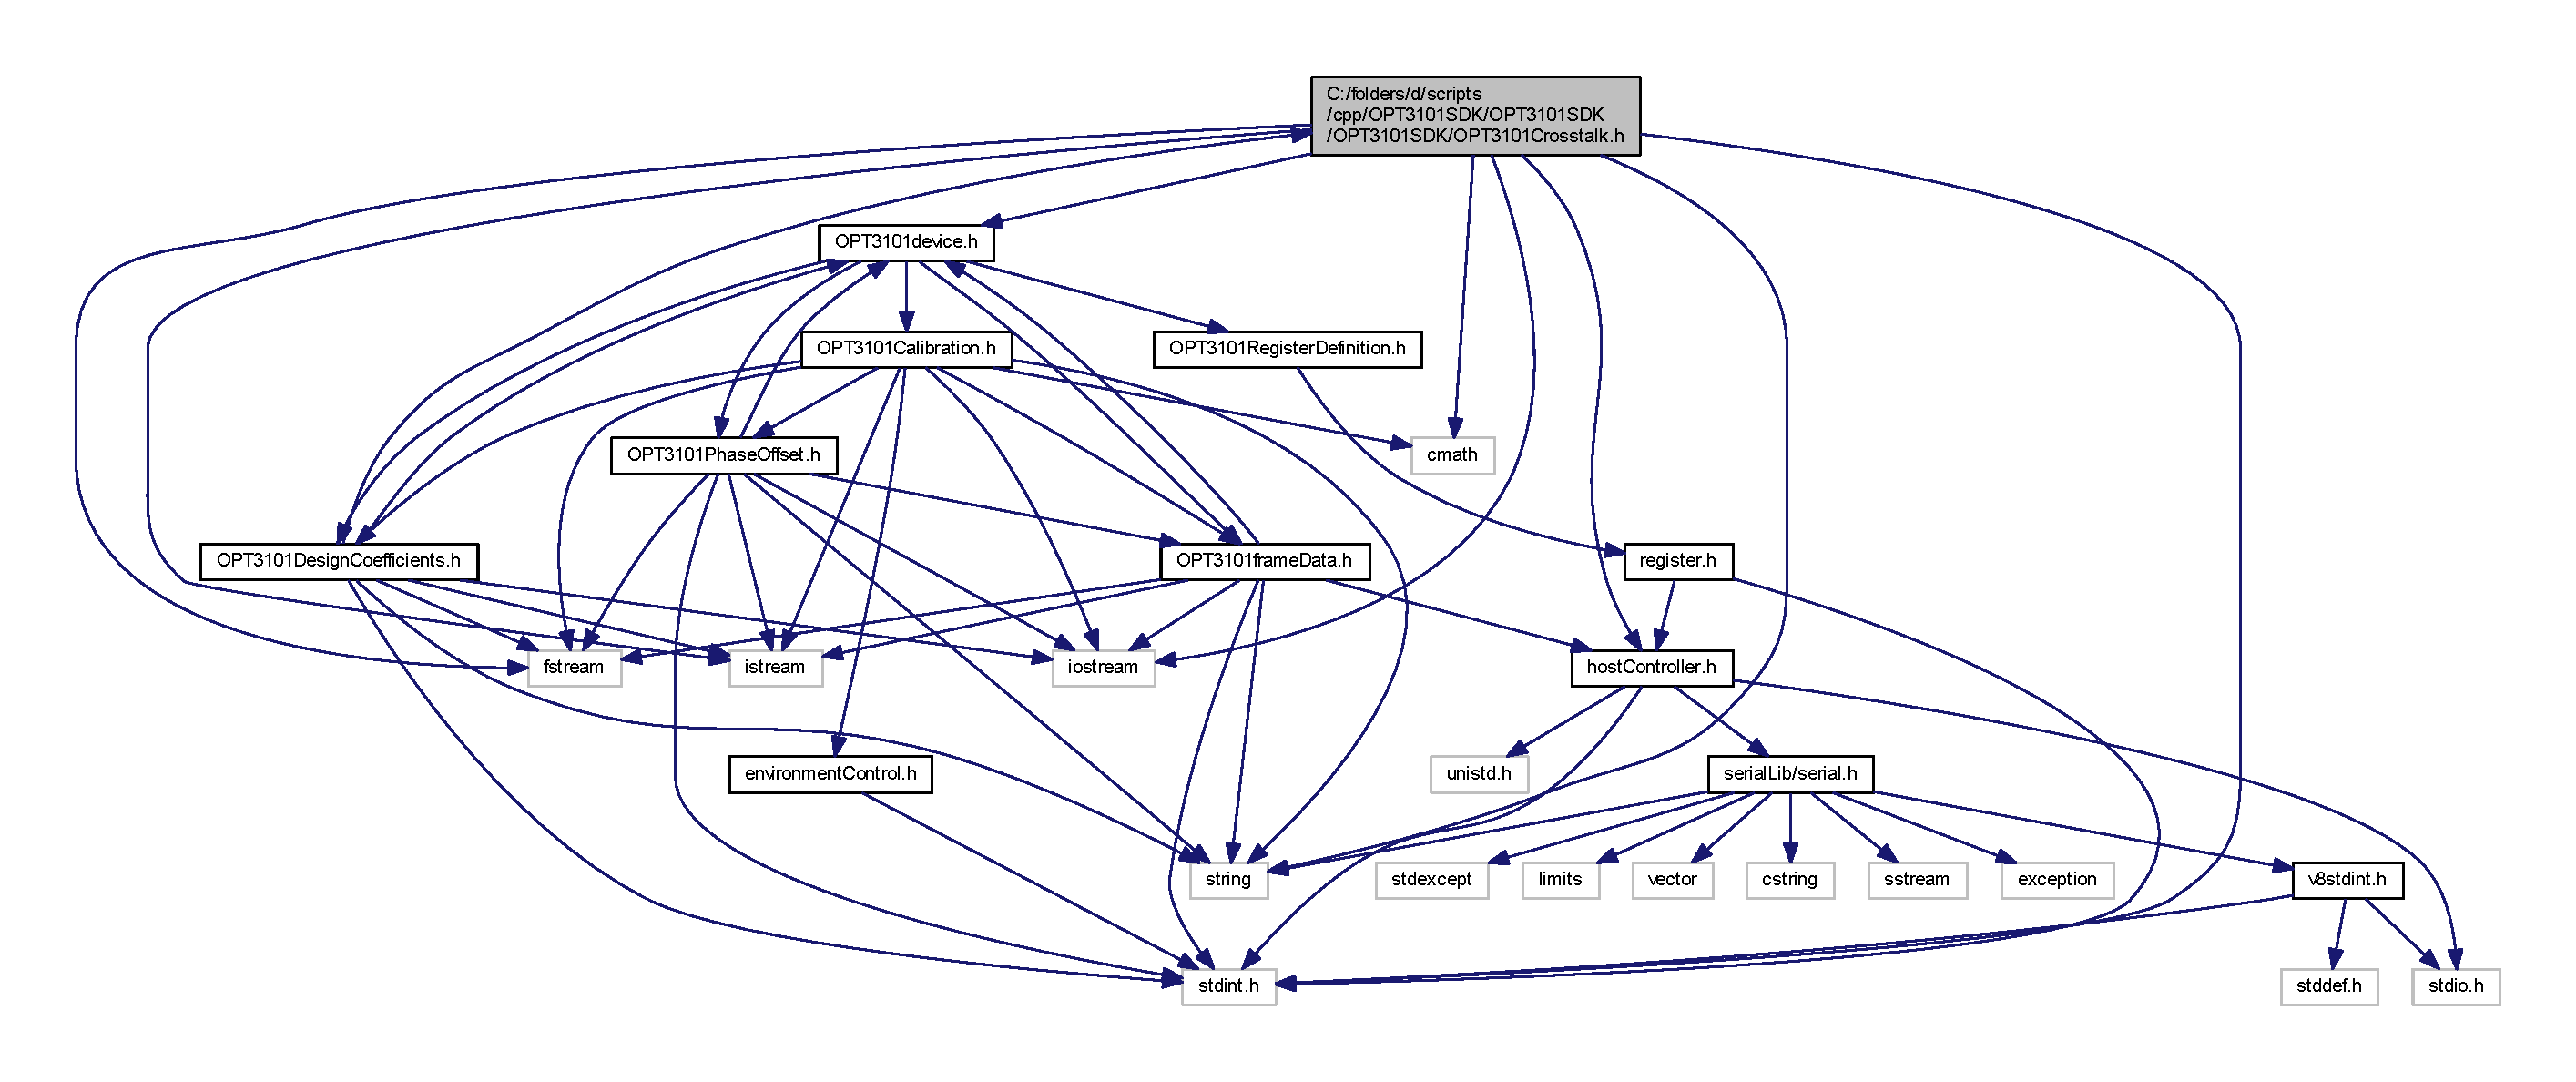
\includegraphics[width=350pt]{_o_p_t3101_crosstalk_8h__incl}
\end{center}
\end{figure}
This graph shows which files directly or indirectly include this file\+:\nopagebreak
\begin{figure}[H]
\begin{center}
\leavevmode
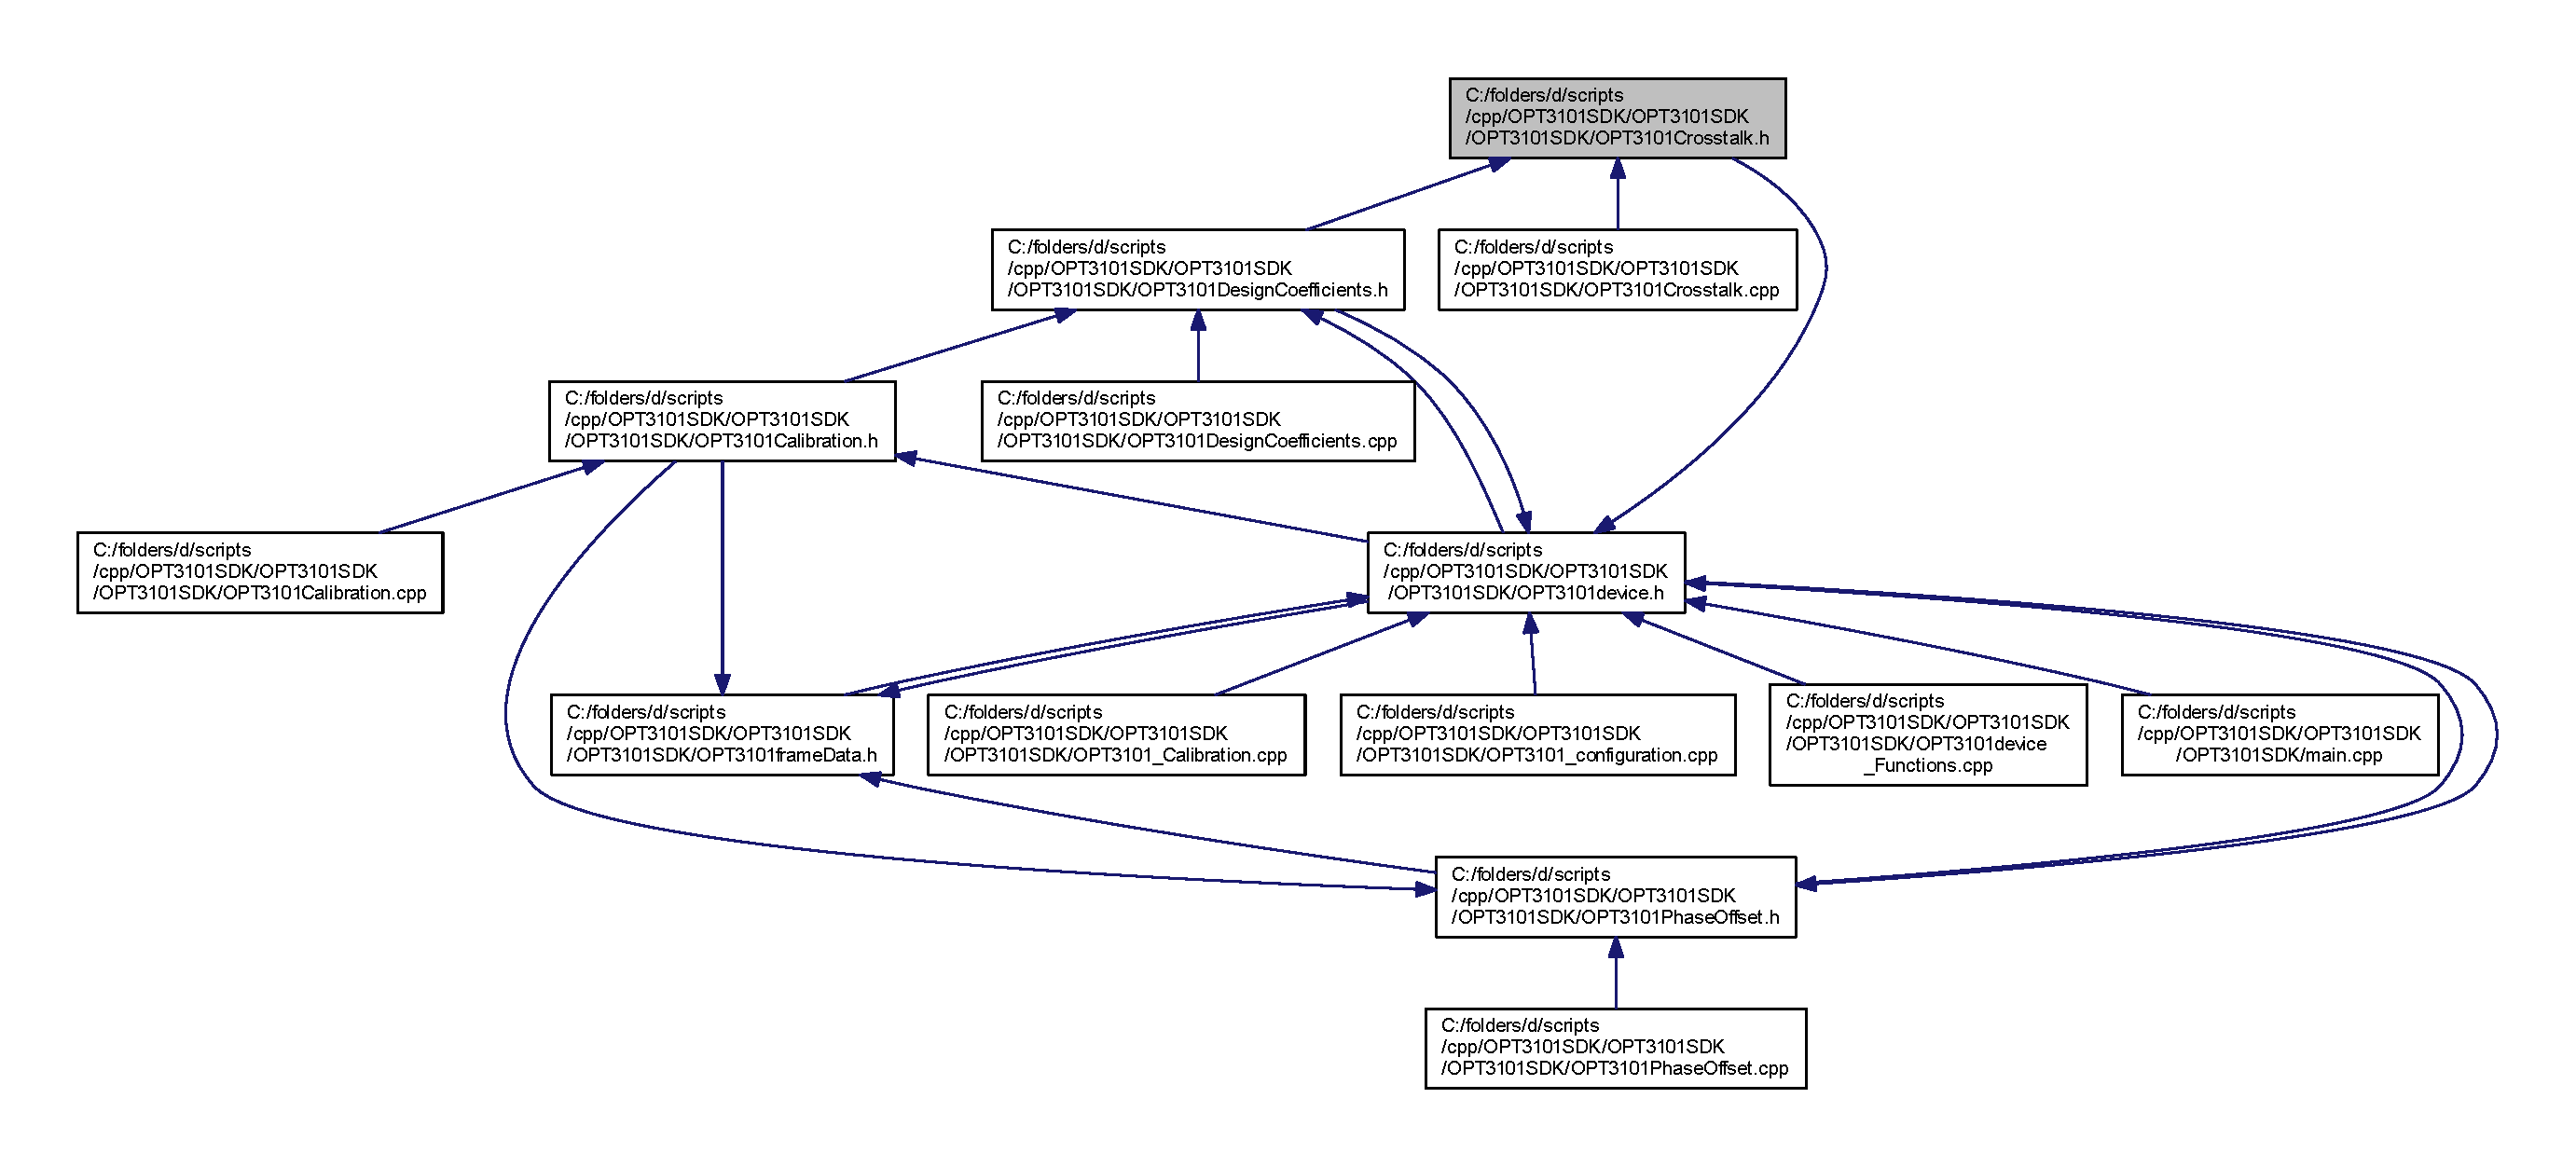
\includegraphics[width=350pt]{_o_p_t3101_crosstalk_8h__dep__incl}
\end{center}
\end{figure}
\subsection*{Classes}
\begin{DoxyCompactItemize}
\item 
class \mbox{\hyperlink{class_o_p_t3101_1_1crosstalk_c}{O\+P\+T3101\+::crosstalkC}}
\begin{DoxyCompactList}\small\item\em Class that holds crosstalk related registers and values. \end{DoxyCompactList}\end{DoxyCompactItemize}
\subsection*{Namespaces}
\begin{DoxyCompactItemize}
\item 
 \mbox{\hyperlink{namespace_o_p_t3101}{O\+P\+T3101}}
\begin{DoxyCompactList}\small\item\em \mbox{\hyperlink{class_o_p_t3101_1_1device}{O\+P\+T3101\+::device}} declaration This is declared here to avoid cyclic reference of classes. \end{DoxyCompactList}\end{DoxyCompactItemize}


\subsection{Detailed Description}
\begin{DoxyAuthor}{Author}
Karthik Rajagopal \href{mailto:krthik@ti.com}{\tt krthik@ti.\+com} 
\end{DoxyAuthor}
\begin{DoxyVersion}{Version}
0.\+8
\end{DoxyVersion}
\hypertarget{register_8h_COPYRIGHT}{}\subsection{C\+O\+P\+Y\+R\+I\+G\+HT}\label{register_8h_COPYRIGHT}
T\+E\+X\+AS I\+N\+S\+T\+R\+U\+M\+E\+N\+TS T\+E\+XT F\+I\+LE L\+I\+C\+E\+N\+SE Copyright (c) 2018 Texas Instruments Incorporated All rights reserved not granted herein. Limited License. Texas Instruments Incorporated grants a world-\/wide, royalty-\/free, non-\/exclusive license under copyrights and patents it now or hereafter owns or controls to make, have made, use, import, offer to sell and sell (\char`\"{}\+Utilize\char`\"{}) this software subject to the terms herein. With respect to the foregoing patent license, such license is granted solely to the extent that any such patent is necessary to Utilize the software alone. The patent license shall not apply to any combinations which include this software, other than combinations with devices manufactured by or for TI (�\+TI Devices�). No hardware patent is licensed hereunder. Redistributions must preserve existing copyright notices and reproduce this license (including the above copyright notice and the disclaimer and (if applicable) source code license limitations below) in the documentation and/or other materials provided with the distribution Redistribution and use in binary form, without modification, are permitted provided that the following conditions are met\+:
\begin{DoxyItemize}
\item No reverse engineering, decompilation, or disassembly of this software is permitted with respect to any software provided in binary form.
\item any redistribution and use are licensed by TI for use only with TI Devices.
\item Nothing shall obligate TI to provide you with source code for the software licensed and provided to you in object code. If software source code is provided to you, modification and redistribution of the source code are permitted provided that the following conditions are met\+:
\item any redistribution and use of the source code, including any resulting derivative works, are licensed by TI for use only with TI Devices.
\item any redistribution and use of any object code compiled from the source code and any resulting derivative works, are licensed by TI for use only with TI Devices. Neither the name of Texas Instruments Incorporated nor the names of its suppliers may be used to endorse or promote products derived from this software without specific prior written permission. D\+I\+S\+C\+L\+A\+I\+M\+ER. T\+H\+IS S\+O\+F\+T\+W\+A\+RE IS P\+R\+O\+V\+I\+D\+ED BY TI A\+ND T\+I�S L\+I\+C\+E\+N\+S\+O\+RS \char`\"{}\+A\+S I\+S\char`\"{} A\+ND A\+NY E\+X\+P\+R\+E\+SS OR I\+M\+P\+L\+I\+ED W\+A\+R\+R\+A\+N\+T\+I\+ES, I\+N\+C\+L\+U\+D\+I\+NG, B\+UT N\+OT L\+I\+M\+I\+T\+ED TO, T\+HE I\+M\+P\+L\+I\+ED W\+A\+R\+R\+A\+N\+T\+I\+ES OF M\+E\+R\+C\+H\+A\+N\+T\+A\+B\+I\+L\+I\+TY A\+ND F\+I\+T\+N\+E\+SS F\+OR A P\+A\+R\+T\+I\+C\+U\+L\+AR P\+U\+R\+P\+O\+SE A\+RE D\+I\+S\+C\+L\+A\+I\+M\+ED. IN NO E\+V\+E\+NT S\+H\+A\+LL TI A\+ND T\+I�S L\+I\+C\+E\+N\+S\+O\+RS BE L\+I\+A\+B\+LE F\+OR A\+NY D\+I\+R\+E\+CT, I\+N\+D\+I\+R\+E\+CT, I\+N\+C\+I\+D\+E\+N\+T\+AL, S\+P\+E\+C\+I\+AL, E\+X\+E\+M\+P\+L\+A\+RY, OR C\+O\+N\+S\+E\+Q\+U\+E\+N\+T\+I\+AL D\+A\+M\+A\+G\+ES (I\+N\+C\+L\+U\+D\+I\+NG, B\+UT N\+OT L\+I\+M\+I\+T\+ED TO, P\+R\+O\+C\+U\+R\+E\+M\+E\+NT OF S\+U\+B\+S\+T\+I\+T\+U\+TE G\+O\+O\+DS OR S\+E\+R\+V\+I\+C\+ES; L\+O\+SS OF U\+SE, D\+A\+TA, OR P\+R\+O\+F\+I\+TS; OR B\+U\+S\+I\+N\+E\+SS I\+N\+T\+E\+R\+R\+U\+P\+T\+I\+ON) H\+O\+W\+E\+V\+ER C\+A\+U\+S\+ED A\+ND ON A\+NY T\+H\+E\+O\+RY OF L\+I\+A\+B\+I\+L\+I\+TY, W\+H\+E\+T\+H\+ER IN C\+O\+N\+T\+R\+A\+CT, S\+T\+R\+I\+CT L\+I\+A\+B\+I\+L\+I\+TY, OR T\+O\+RT (I\+N\+C\+L\+U\+D\+I\+NG N\+E\+G\+L\+I\+G\+E\+N\+CE OR O\+T\+H\+E\+R\+W\+I\+SE) A\+R\+I\+S\+I\+NG IN A\+NY W\+AY O\+UT OF T\+HE U\+SE OF T\+H\+IS S\+O\+F\+T\+W\+A\+RE, E\+V\+EN IF A\+D\+V\+I\+S\+ED OF T\+HE P\+O\+S\+S\+I\+B\+I\+L\+I\+TY OF S\+U\+CH D\+A\+M\+A\+GE.
\end{DoxyItemize}\hypertarget{register_8h_DESCRIPTION}{}\subsection{D\+E\+S\+C\+R\+I\+P\+T\+I\+ON}\label{register_8h_DESCRIPTION}
This file contains the \mbox{\hyperlink{class_o_p_t3101_1_1crosstalk_c}{O\+P\+T3101\+::crosstalkC}} class declaration 
\hypertarget{_o_p_t3101_design_coefficients_8cpp}{}\section{C\+:/folders/d/scripts/cpp/\+O\+P\+T3101\+S\+D\+K/\+O\+P\+T3101\+S\+D\+K/\+O\+P\+T3101\+S\+D\+K/\+O\+P\+T3101\+Design\+Coefficients.cpp File Reference}
\label{_o_p_t3101_design_coefficients_8cpp}\index{C\+:/folders/d/scripts/cpp/\+O\+P\+T3101\+S\+D\+K/\+O\+P\+T3101\+S\+D\+K/\+O\+P\+T3101\+S\+D\+K/\+O\+P\+T3101\+Design\+Coefficients.\+cpp@{C\+:/folders/d/scripts/cpp/\+O\+P\+T3101\+S\+D\+K/\+O\+P\+T3101\+S\+D\+K/\+O\+P\+T3101\+S\+D\+K/\+O\+P\+T3101\+Design\+Coefficients.\+cpp}}
{\ttfamily \#include \char`\"{}O\+P\+T3101\+Design\+Coefficients.\+h\char`\"{}}\newline
Include dependency graph for O\+P\+T3101\+Design\+Coefficients.\+cpp\+:\nopagebreak
\begin{figure}[H]
\begin{center}
\leavevmode
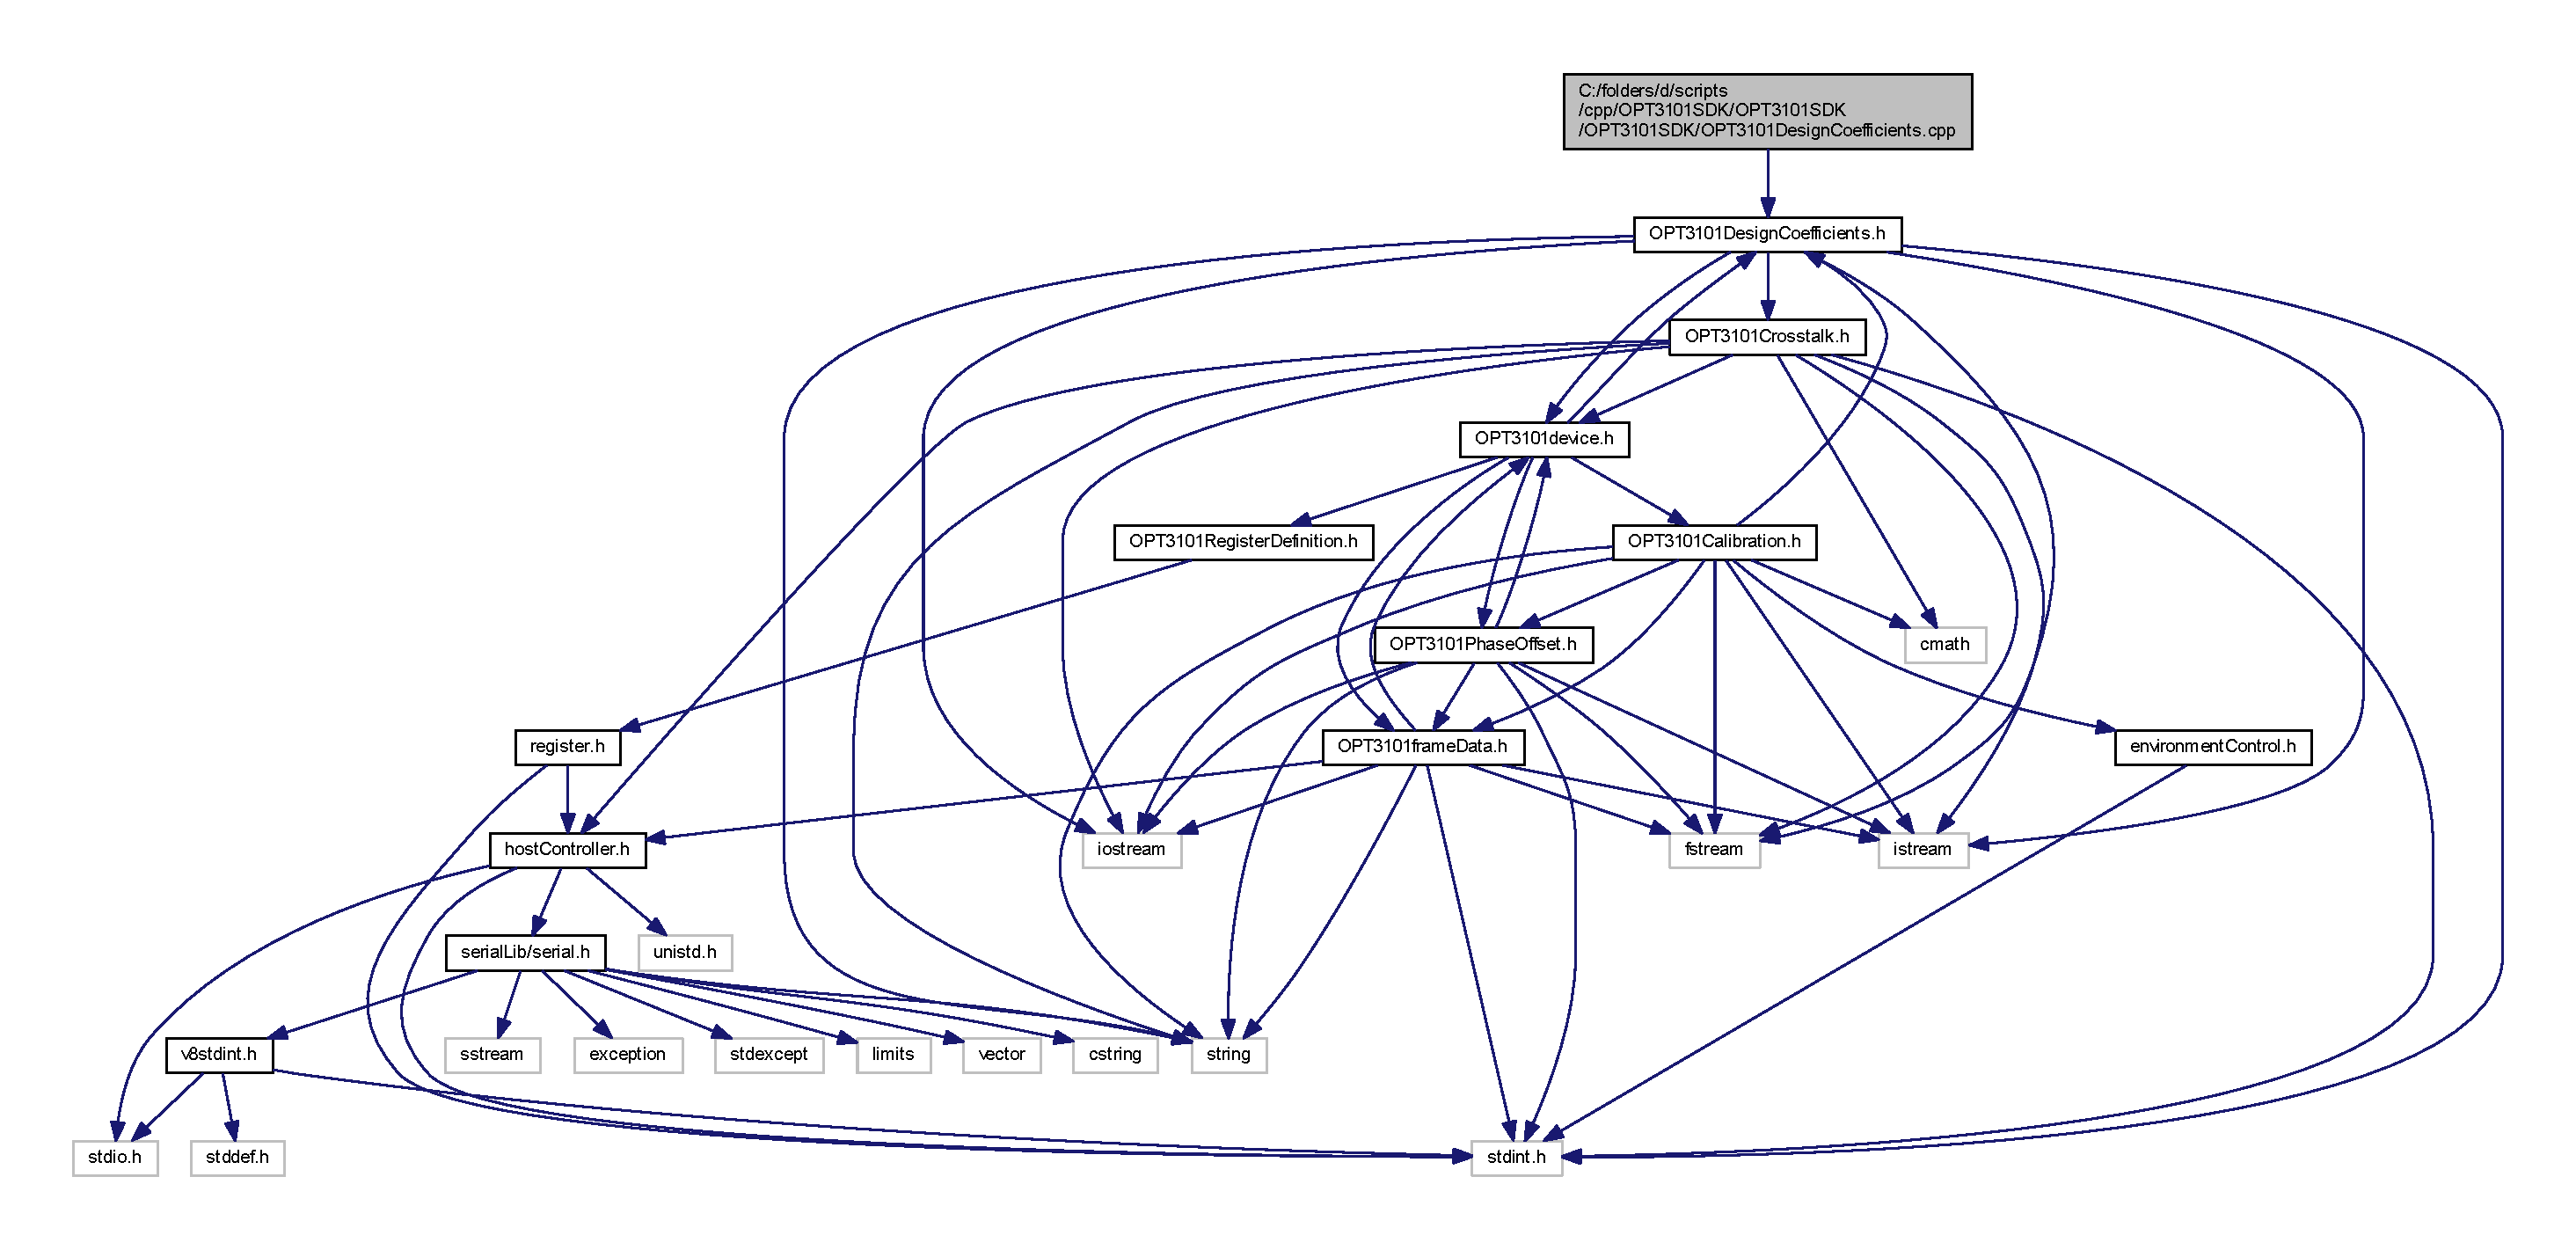
\includegraphics[width=350pt]{_o_p_t3101_design_coefficients_8cpp__incl}
\end{center}
\end{figure}


\subsection{Detailed Description}
\begin{DoxyAuthor}{Author}
Karthik Rajagopal \href{mailto:krthik@ti.com}{\tt krthik@ti.\+com} 
\end{DoxyAuthor}
\begin{DoxyVersion}{Version}
0.\+8
\end{DoxyVersion}
\hypertarget{register_8h_COPYRIGHT}{}\subsection{C\+O\+P\+Y\+R\+I\+G\+HT}\label{register_8h_COPYRIGHT}
T\+E\+X\+AS I\+N\+S\+T\+R\+U\+M\+E\+N\+TS T\+E\+XT F\+I\+LE L\+I\+C\+E\+N\+SE Copyright (c) 2018 Texas Instruments Incorporated All rights reserved not granted herein. Limited License. Texas Instruments Incorporated grants a world-\/wide, royalty-\/free, non-\/exclusive license under copyrights and patents it now or hereafter owns or controls to make, have made, use, import, offer to sell and sell (\char`\"{}\+Utilize\char`\"{}) this software subject to the terms herein. With respect to the foregoing patent license, such license is granted solely to the extent that any such patent is necessary to Utilize the software alone. The patent license shall not apply to any combinations which include this software, other than combinations with devices manufactured by or for TI (�\+TI Devices�). No hardware patent is licensed hereunder. Redistributions must preserve existing copyright notices and reproduce this license (including the above copyright notice and the disclaimer and (if applicable) source code license limitations below) in the documentation and/or other materials provided with the distribution Redistribution and use in binary form, without modification, are permitted provided that the following conditions are met\+:
\begin{DoxyItemize}
\item No reverse engineering, decompilation, or disassembly of this software is permitted with respect to any software provided in binary form.
\item any redistribution and use are licensed by TI for use only with TI Devices.
\item Nothing shall obligate TI to provide you with source code for the software licensed and provided to you in object code. If software source code is provided to you, modification and redistribution of the source code are permitted provided that the following conditions are met\+:
\item any redistribution and use of the source code, including any resulting derivative works, are licensed by TI for use only with TI Devices.
\item any redistribution and use of any object code compiled from the source code and any resulting derivative works, are licensed by TI for use only with TI Devices. Neither the name of Texas Instruments Incorporated nor the names of its suppliers may be used to endorse or promote products derived from this software without specific prior written permission. D\+I\+S\+C\+L\+A\+I\+M\+ER. T\+H\+IS S\+O\+F\+T\+W\+A\+RE IS P\+R\+O\+V\+I\+D\+ED BY TI A\+ND T\+I�S L\+I\+C\+E\+N\+S\+O\+RS \char`\"{}\+A\+S I\+S\char`\"{} A\+ND A\+NY E\+X\+P\+R\+E\+SS OR I\+M\+P\+L\+I\+ED W\+A\+R\+R\+A\+N\+T\+I\+ES, I\+N\+C\+L\+U\+D\+I\+NG, B\+UT N\+OT L\+I\+M\+I\+T\+ED TO, T\+HE I\+M\+P\+L\+I\+ED W\+A\+R\+R\+A\+N\+T\+I\+ES OF M\+E\+R\+C\+H\+A\+N\+T\+A\+B\+I\+L\+I\+TY A\+ND F\+I\+T\+N\+E\+SS F\+OR A P\+A\+R\+T\+I\+C\+U\+L\+AR P\+U\+R\+P\+O\+SE A\+RE D\+I\+S\+C\+L\+A\+I\+M\+ED. IN NO E\+V\+E\+NT S\+H\+A\+LL TI A\+ND T\+I�S L\+I\+C\+E\+N\+S\+O\+RS BE L\+I\+A\+B\+LE F\+OR A\+NY D\+I\+R\+E\+CT, I\+N\+D\+I\+R\+E\+CT, I\+N\+C\+I\+D\+E\+N\+T\+AL, S\+P\+E\+C\+I\+AL, E\+X\+E\+M\+P\+L\+A\+RY, OR C\+O\+N\+S\+E\+Q\+U\+E\+N\+T\+I\+AL D\+A\+M\+A\+G\+ES (I\+N\+C\+L\+U\+D\+I\+NG, B\+UT N\+OT L\+I\+M\+I\+T\+ED TO, P\+R\+O\+C\+U\+R\+E\+M\+E\+NT OF S\+U\+B\+S\+T\+I\+T\+U\+TE G\+O\+O\+DS OR S\+E\+R\+V\+I\+C\+ES; L\+O\+SS OF U\+SE, D\+A\+TA, OR P\+R\+O\+F\+I\+TS; OR B\+U\+S\+I\+N\+E\+SS I\+N\+T\+E\+R\+R\+U\+P\+T\+I\+ON) H\+O\+W\+E\+V\+ER C\+A\+U\+S\+ED A\+ND ON A\+NY T\+H\+E\+O\+RY OF L\+I\+A\+B\+I\+L\+I\+TY, W\+H\+E\+T\+H\+ER IN C\+O\+N\+T\+R\+A\+CT, S\+T\+R\+I\+CT L\+I\+A\+B\+I\+L\+I\+TY, OR T\+O\+RT (I\+N\+C\+L\+U\+D\+I\+NG N\+E\+G\+L\+I\+G\+E\+N\+CE OR O\+T\+H\+E\+R\+W\+I\+SE) A\+R\+I\+S\+I\+NG IN A\+NY W\+AY O\+UT OF T\+HE U\+SE OF T\+H\+IS S\+O\+F\+T\+W\+A\+RE, E\+V\+EN IF A\+D\+V\+I\+S\+ED OF T\+HE P\+O\+S\+S\+I\+B\+I\+L\+I\+TY OF S\+U\+CH D\+A\+M\+A\+GE.
\end{DoxyItemize}\hypertarget{register_8h_DESCRIPTION}{}\subsection{D\+E\+S\+C\+R\+I\+P\+T\+I\+ON}\label{register_8h_DESCRIPTION}
The file contains methods definitions for classes \mbox{\hyperlink{class_o_p_t3101_1_1crosstalk_temp_coff_c}{O\+P\+T3101\+::crosstalk\+Temp\+CoffC}} \mbox{\hyperlink{class_o_p_t3101_1_1calibration_c}{O\+P\+T3101\+::calibrationC}} \mbox{\hyperlink{class_o_p_t3101_1_1phase_ambient_coff_c}{O\+P\+T3101\+::phase\+Ambient\+CoffC}} \mbox{\hyperlink{class_o_p_t3101_1_1phase_temp_coff_c}{O\+P\+T3101\+::phase\+Temp\+CoffC}} 
\hypertarget{_o_p_t3101_design_coefficients_8h}{}\section{C\+:/folders/d/scripts/cpp/\+O\+P\+T3101\+S\+D\+K/\+O\+P\+T3101\+S\+D\+K/\+O\+P\+T3101\+S\+D\+K/\+O\+P\+T3101\+Design\+Coefficients.h File Reference}
\label{_o_p_t3101_design_coefficients_8h}\index{C\+:/folders/d/scripts/cpp/\+O\+P\+T3101\+S\+D\+K/\+O\+P\+T3101\+S\+D\+K/\+O\+P\+T3101\+S\+D\+K/\+O\+P\+T3101\+Design\+Coefficients.\+h@{C\+:/folders/d/scripts/cpp/\+O\+P\+T3101\+S\+D\+K/\+O\+P\+T3101\+S\+D\+K/\+O\+P\+T3101\+S\+D\+K/\+O\+P\+T3101\+Design\+Coefficients.\+h}}
{\ttfamily \#include $<$stdint.\+h$>$}\newline
{\ttfamily \#include \char`\"{}O\+P\+T3101device.\+h\char`\"{}}\newline
{\ttfamily \#include \char`\"{}O\+P\+T3101\+Crosstalk.\+h\char`\"{}}\newline
{\ttfamily \#include $<$fstream$>$}\newline
{\ttfamily \#include $<$iostream$>$}\newline
{\ttfamily \#include $<$istream$>$}\newline
{\ttfamily \#include $<$string$>$}\newline
Include dependency graph for O\+P\+T3101\+Design\+Coefficients.\+h\+:\nopagebreak
\begin{figure}[H]
\begin{center}
\leavevmode
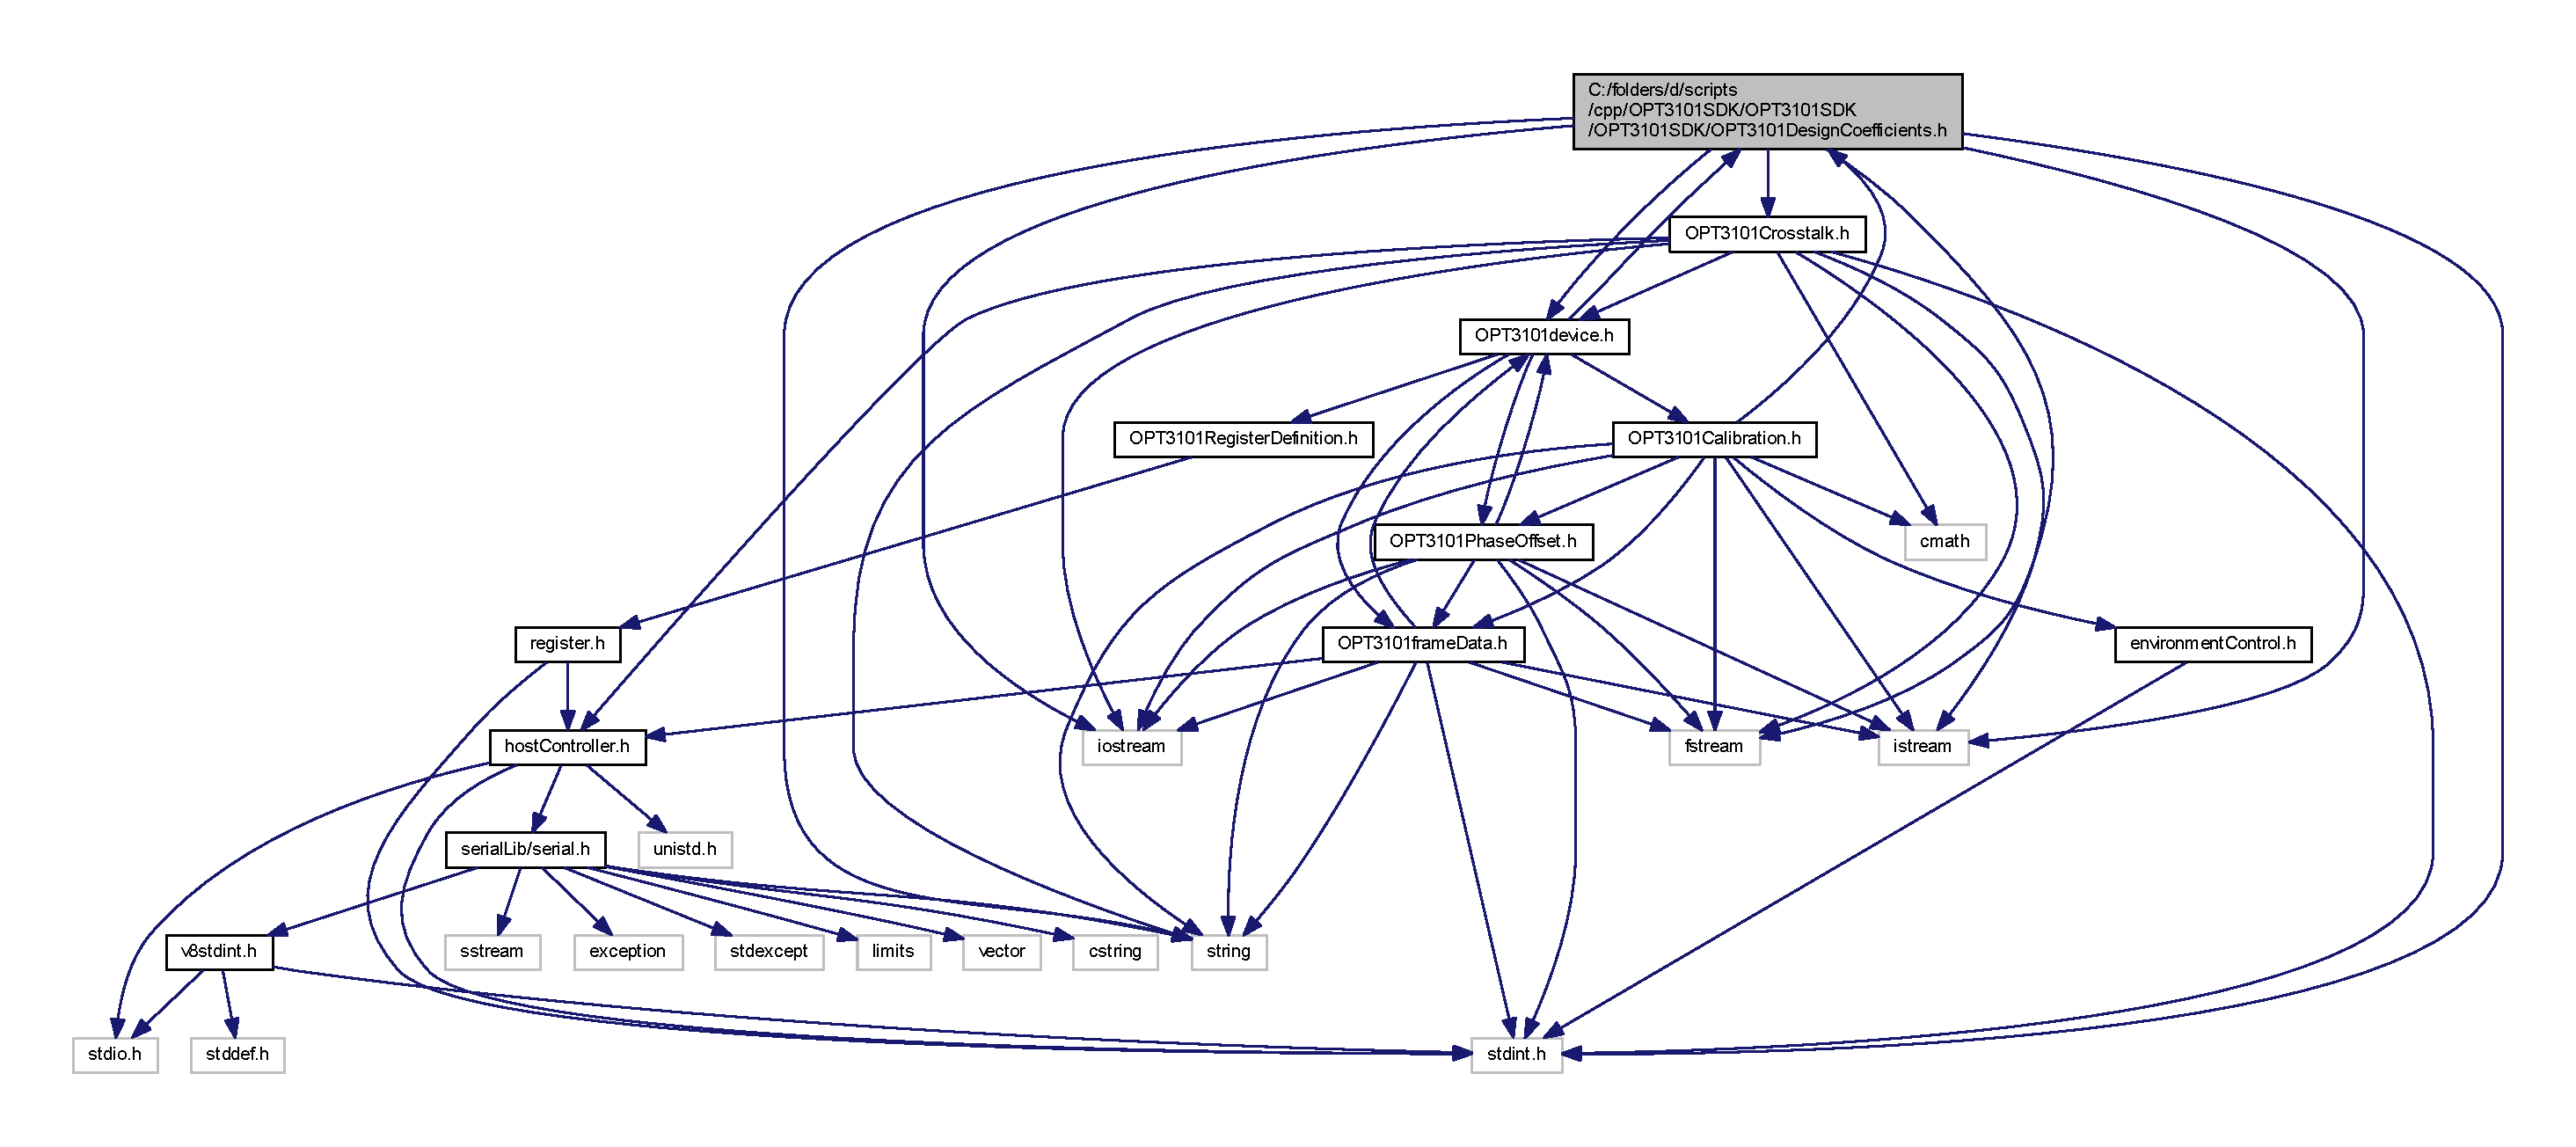
\includegraphics[width=350pt]{_o_p_t3101_design_coefficients_8h__incl}
\end{center}
\end{figure}
This graph shows which files directly or indirectly include this file\+:\nopagebreak
\begin{figure}[H]
\begin{center}
\leavevmode
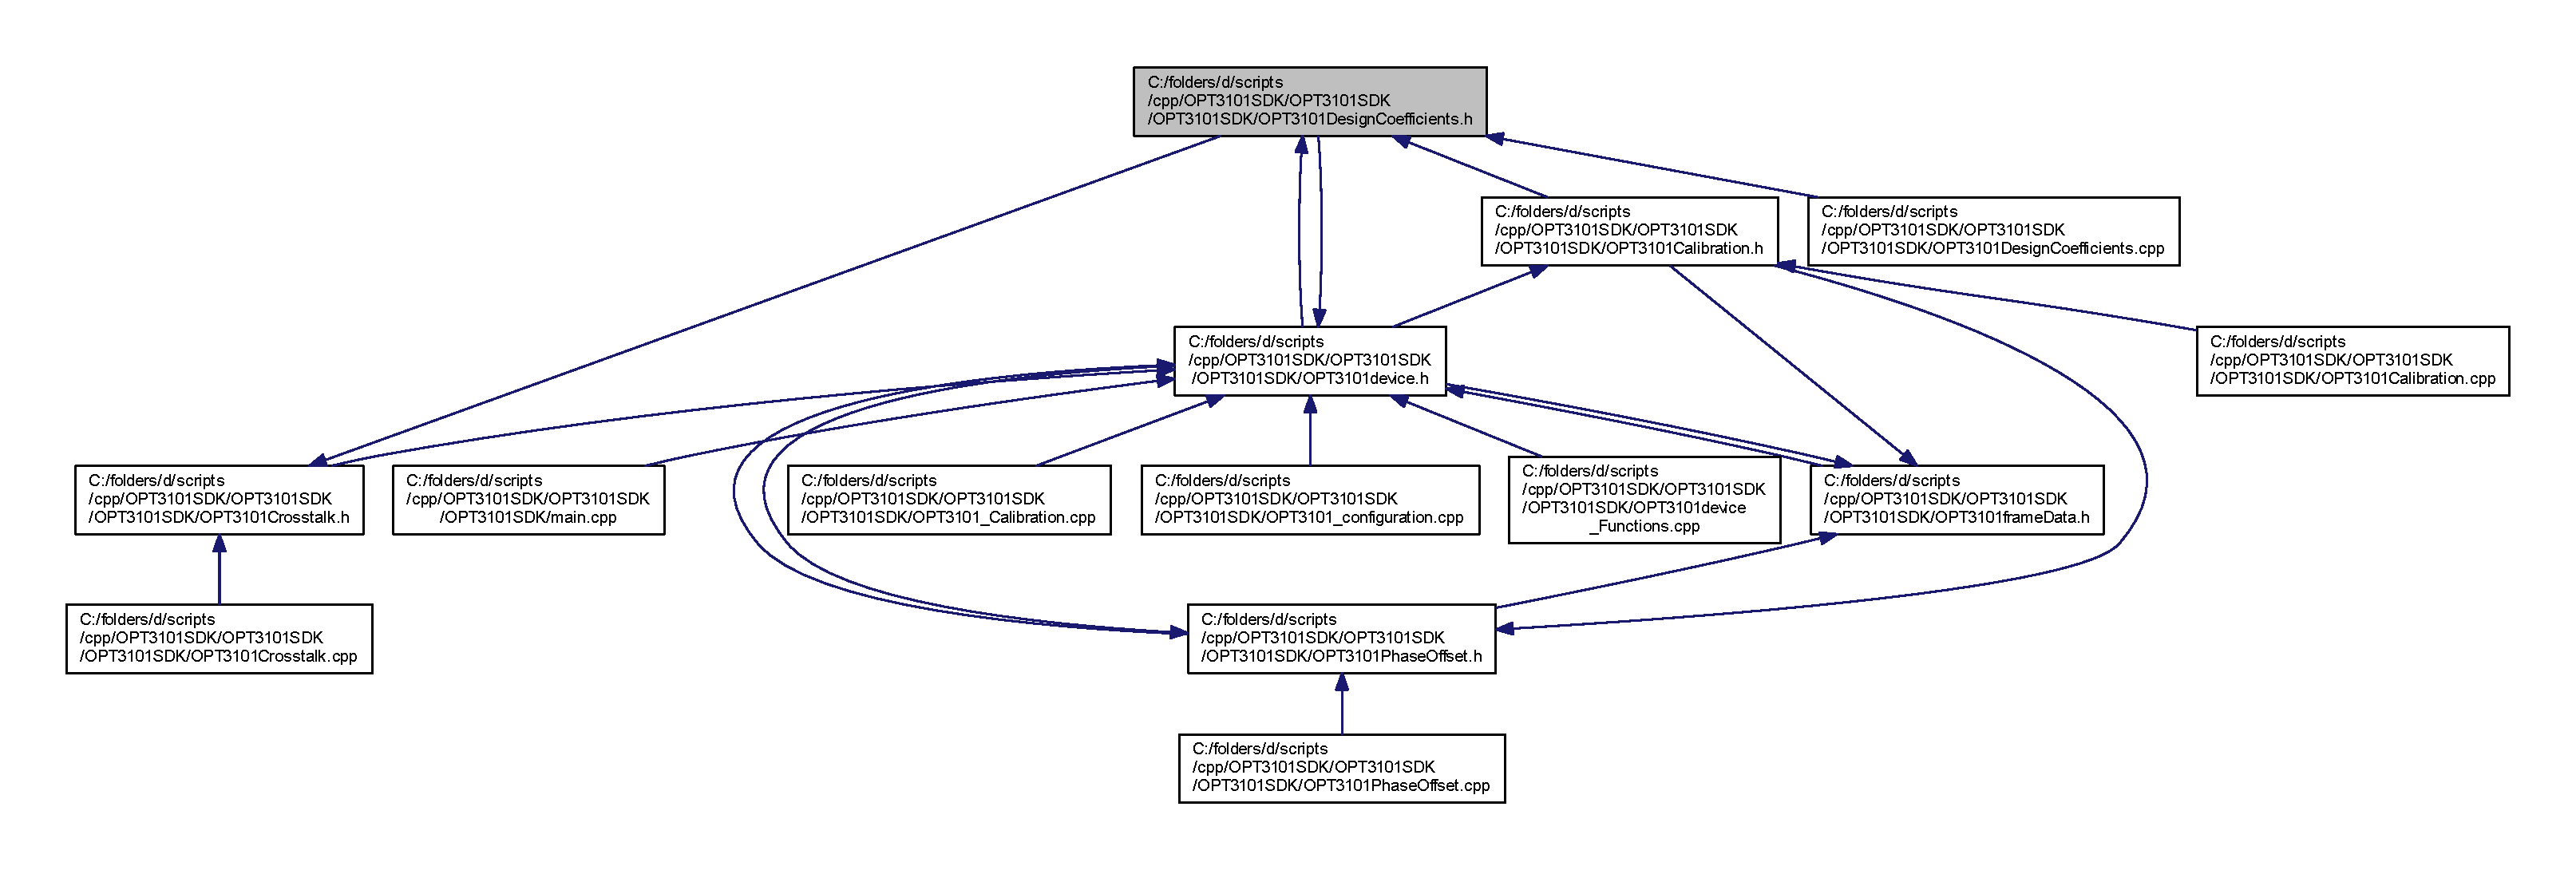
\includegraphics[width=350pt]{_o_p_t3101_design_coefficients_8h__dep__incl}
\end{center}
\end{figure}
\subsection*{Classes}
\begin{DoxyCompactItemize}
\item 
class \mbox{\hyperlink{class_o_p_t3101_1_1crosstalk_temp_coff_c}{O\+P\+T3101\+::crosstalk\+Temp\+CoffC}}
\begin{DoxyCompactList}\small\item\em Class that holds crosstalk temperature coefficient related registers and values. \end{DoxyCompactList}\item 
class \mbox{\hyperlink{class_o_p_t3101_1_1phase_temp_coff_c}{O\+P\+T3101\+::phase\+Temp\+CoffC}}
\begin{DoxyCompactList}\small\item\em Class that holds phase temperature coefficient related registers and values. \end{DoxyCompactList}\item 
class \mbox{\hyperlink{class_o_p_t3101_1_1phase_ambient_coff_c}{O\+P\+T3101\+::phase\+Ambient\+CoffC}}
\begin{DoxyCompactList}\small\item\em Class that holds ambient phase coefficient related registers and values. \end{DoxyCompactList}\end{DoxyCompactItemize}
\subsection*{Namespaces}
\begin{DoxyCompactItemize}
\item 
 \mbox{\hyperlink{namespace_o_p_t3101}{O\+P\+T3101}}
\begin{DoxyCompactList}\small\item\em \mbox{\hyperlink{class_o_p_t3101_1_1device}{O\+P\+T3101\+::device}} declaration This is declared here to avoid cyclic reference of classes. \end{DoxyCompactList}\end{DoxyCompactItemize}


\subsection{Detailed Description}
\begin{DoxyAuthor}{Author}
Karthik Rajagopal \href{mailto:krthik@ti.com}{\tt krthik@ti.\+com} 
\end{DoxyAuthor}
\begin{DoxyVersion}{Version}
0.\+8
\end{DoxyVersion}
\hypertarget{register_8h_COPYRIGHT}{}\subsection{C\+O\+P\+Y\+R\+I\+G\+HT}\label{register_8h_COPYRIGHT}
T\+E\+X\+AS I\+N\+S\+T\+R\+U\+M\+E\+N\+TS T\+E\+XT F\+I\+LE L\+I\+C\+E\+N\+SE Copyright (c) 2018 Texas Instruments Incorporated All rights reserved not granted herein. Limited License. Texas Instruments Incorporated grants a world-\/wide, royalty-\/free, non-\/exclusive license under copyrights and patents it now or hereafter owns or controls to make, have made, use, import, offer to sell and sell (\char`\"{}\+Utilize\char`\"{}) this software subject to the terms herein. With respect to the foregoing patent license, such license is granted solely to the extent that any such patent is necessary to Utilize the software alone. The patent license shall not apply to any combinations which include this software, other than combinations with devices manufactured by or for TI (�\+TI Devices�). No hardware patent is licensed hereunder. Redistributions must preserve existing copyright notices and reproduce this license (including the above copyright notice and the disclaimer and (if applicable) source code license limitations below) in the documentation and/or other materials provided with the distribution Redistribution and use in binary form, without modification, are permitted provided that the following conditions are met\+:
\begin{DoxyItemize}
\item No reverse engineering, decompilation, or disassembly of this software is permitted with respect to any software provided in binary form.
\item any redistribution and use are licensed by TI for use only with TI Devices.
\item Nothing shall obligate TI to provide you with source code for the software licensed and provided to you in object code. If software source code is provided to you, modification and redistribution of the source code are permitted provided that the following conditions are met\+:
\item any redistribution and use of the source code, including any resulting derivative works, are licensed by TI for use only with TI Devices.
\item any redistribution and use of any object code compiled from the source code and any resulting derivative works, are licensed by TI for use only with TI Devices. Neither the name of Texas Instruments Incorporated nor the names of its suppliers may be used to endorse or promote products derived from this software without specific prior written permission. D\+I\+S\+C\+L\+A\+I\+M\+ER. T\+H\+IS S\+O\+F\+T\+W\+A\+RE IS P\+R\+O\+V\+I\+D\+ED BY TI A\+ND T\+I�S L\+I\+C\+E\+N\+S\+O\+RS \char`\"{}\+A\+S I\+S\char`\"{} A\+ND A\+NY E\+X\+P\+R\+E\+SS OR I\+M\+P\+L\+I\+ED W\+A\+R\+R\+A\+N\+T\+I\+ES, I\+N\+C\+L\+U\+D\+I\+NG, B\+UT N\+OT L\+I\+M\+I\+T\+ED TO, T\+HE I\+M\+P\+L\+I\+ED W\+A\+R\+R\+A\+N\+T\+I\+ES OF M\+E\+R\+C\+H\+A\+N\+T\+A\+B\+I\+L\+I\+TY A\+ND F\+I\+T\+N\+E\+SS F\+OR A P\+A\+R\+T\+I\+C\+U\+L\+AR P\+U\+R\+P\+O\+SE A\+RE D\+I\+S\+C\+L\+A\+I\+M\+ED. IN NO E\+V\+E\+NT S\+H\+A\+LL TI A\+ND T\+I�S L\+I\+C\+E\+N\+S\+O\+RS BE L\+I\+A\+B\+LE F\+OR A\+NY D\+I\+R\+E\+CT, I\+N\+D\+I\+R\+E\+CT, I\+N\+C\+I\+D\+E\+N\+T\+AL, S\+P\+E\+C\+I\+AL, E\+X\+E\+M\+P\+L\+A\+RY, OR C\+O\+N\+S\+E\+Q\+U\+E\+N\+T\+I\+AL D\+A\+M\+A\+G\+ES (I\+N\+C\+L\+U\+D\+I\+NG, B\+UT N\+OT L\+I\+M\+I\+T\+ED TO, P\+R\+O\+C\+U\+R\+E\+M\+E\+NT OF S\+U\+B\+S\+T\+I\+T\+U\+TE G\+O\+O\+DS OR S\+E\+R\+V\+I\+C\+ES; L\+O\+SS OF U\+SE, D\+A\+TA, OR P\+R\+O\+F\+I\+TS; OR B\+U\+S\+I\+N\+E\+SS I\+N\+T\+E\+R\+R\+U\+P\+T\+I\+ON) H\+O\+W\+E\+V\+ER C\+A\+U\+S\+ED A\+ND ON A\+NY T\+H\+E\+O\+RY OF L\+I\+A\+B\+I\+L\+I\+TY, W\+H\+E\+T\+H\+ER IN C\+O\+N\+T\+R\+A\+CT, S\+T\+R\+I\+CT L\+I\+A\+B\+I\+L\+I\+TY, OR T\+O\+RT (I\+N\+C\+L\+U\+D\+I\+NG N\+E\+G\+L\+I\+G\+E\+N\+CE OR O\+T\+H\+E\+R\+W\+I\+SE) A\+R\+I\+S\+I\+NG IN A\+NY W\+AY O\+UT OF T\+HE U\+SE OF T\+H\+IS S\+O\+F\+T\+W\+A\+RE, E\+V\+EN IF A\+D\+V\+I\+S\+ED OF T\+HE P\+O\+S\+S\+I\+B\+I\+L\+I\+TY OF S\+U\+CH D\+A\+M\+A\+GE.
\end{DoxyItemize}\hypertarget{register_8h_DESCRIPTION}{}\subsection{D\+E\+S\+C\+R\+I\+P\+T\+I\+ON}\label{register_8h_DESCRIPTION}
This file contains class declarations \mbox{\hyperlink{class_o_p_t3101_1_1crosstalk_temp_coff_c}{O\+P\+T3101\+::crosstalk\+Temp\+CoffC}} \mbox{\hyperlink{class_o_p_t3101_1_1phase_temp_coff_c}{O\+P\+T3101\+::phase\+Temp\+CoffC}} \mbox{\hyperlink{class_o_p_t3101_1_1phase_ambient_coff_c}{O\+P\+T3101\+::phase\+Ambient\+CoffC}} . These are design coefficients required for various calibration steps. 
\hypertarget{_o_p_t3101device_8h}{}\section{C\+:/folders/d/scripts/cpp/\+O\+P\+T3101\+S\+D\+K/\+O\+P\+T3101\+S\+D\+K/\+O\+P\+T3101\+S\+D\+K/\+O\+P\+T3101device.h File Reference}
\label{_o_p_t3101device_8h}\index{C\+:/folders/d/scripts/cpp/\+O\+P\+T3101\+S\+D\+K/\+O\+P\+T3101\+S\+D\+K/\+O\+P\+T3101\+S\+D\+K/\+O\+P\+T3101device.\+h@{C\+:/folders/d/scripts/cpp/\+O\+P\+T3101\+S\+D\+K/\+O\+P\+T3101\+S\+D\+K/\+O\+P\+T3101\+S\+D\+K/\+O\+P\+T3101device.\+h}}
{\ttfamily \#include \char`\"{}O\+P\+T3101\+Register\+Definition.\+h\char`\"{}}\newline
{\ttfamily \#include \char`\"{}O\+P\+T3101\+Calibration.\+h\char`\"{}}\newline
{\ttfamily \#include \char`\"{}O\+P\+T3101\+Design\+Coefficients.\+h\char`\"{}}\newline
{\ttfamily \#include \char`\"{}O\+P\+T3101\+Phase\+Offset.\+h\char`\"{}}\newline
{\ttfamily \#include \char`\"{}O\+P\+T3101frame\+Data.\+h\char`\"{}}\newline
Include dependency graph for O\+P\+T3101device.\+h\+:\nopagebreak
\begin{figure}[H]
\begin{center}
\leavevmode
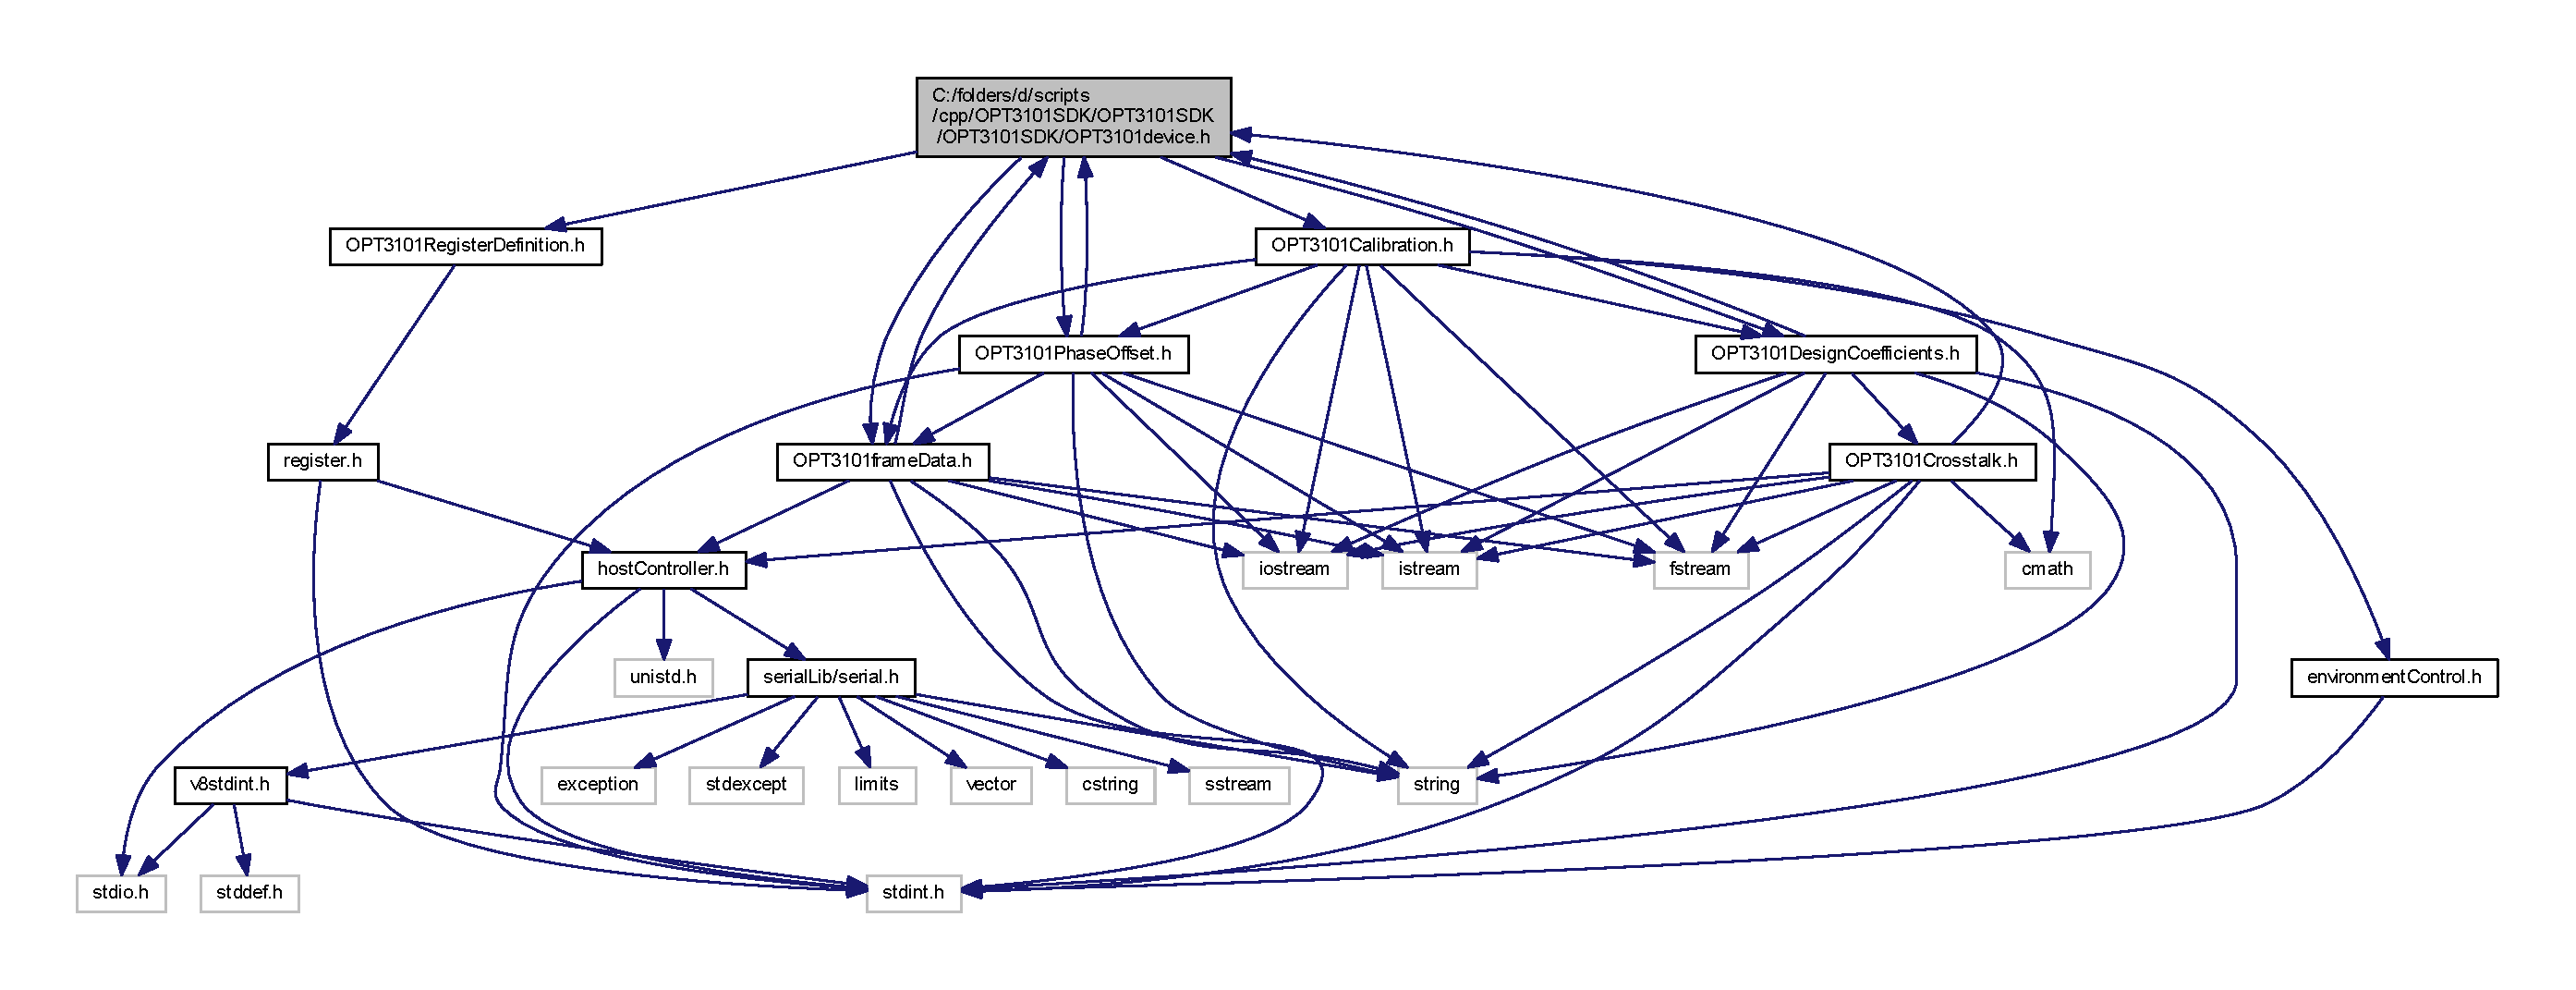
\includegraphics[width=350pt]{_o_p_t3101device_8h__incl}
\end{center}
\end{figure}
This graph shows which files directly or indirectly include this file\+:\nopagebreak
\begin{figure}[H]
\begin{center}
\leavevmode
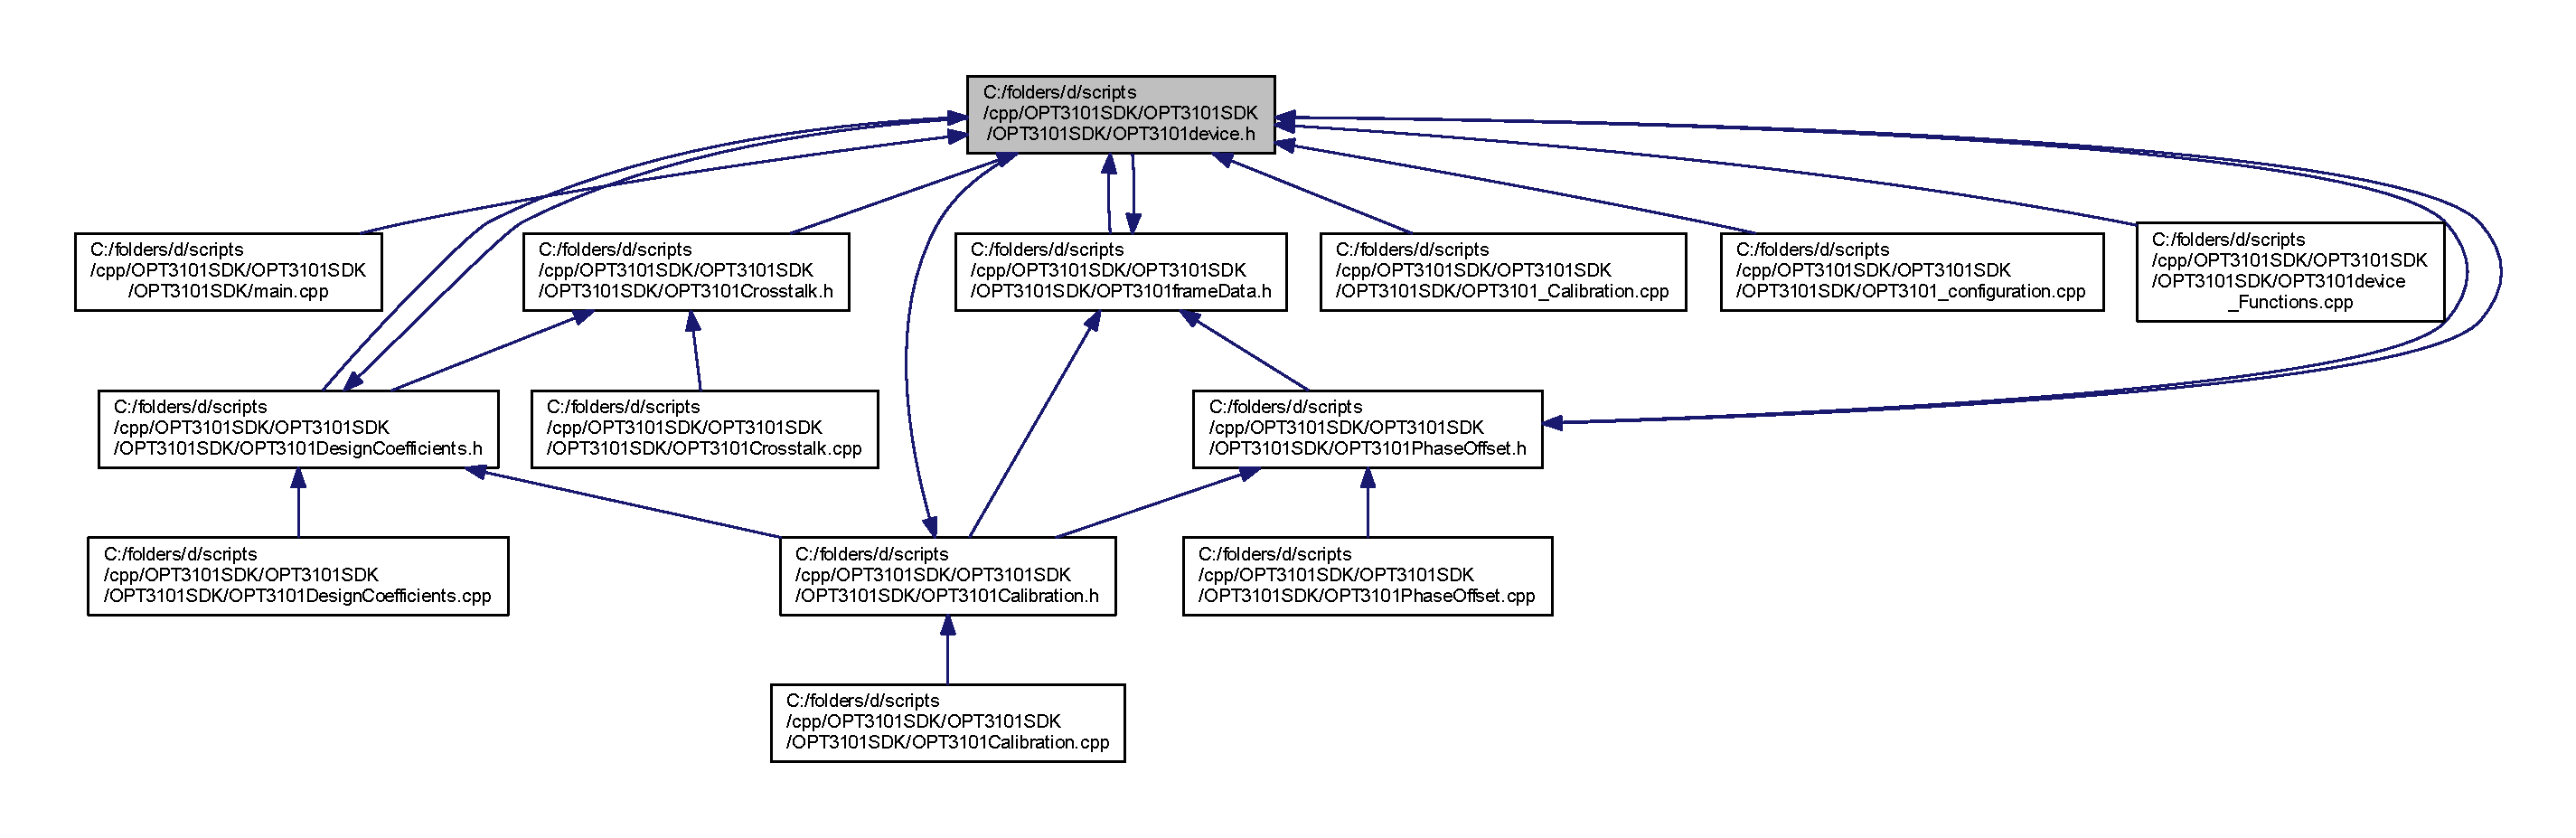
\includegraphics[width=350pt]{_o_p_t3101device_8h__dep__incl}
\end{center}
\end{figure}
\subsection*{Classes}
\begin{DoxyCompactItemize}
\item 
class \mbox{\hyperlink{class_o_p_t3101_1_1device}{O\+P\+T3101\+::device}}
\begin{DoxyCompactList}\small\item\em This is the master class that integrates all the O\+P\+T3101\+S\+DK functions. \end{DoxyCompactList}\end{DoxyCompactItemize}
\subsection*{Namespaces}
\begin{DoxyCompactItemize}
\item 
 \mbox{\hyperlink{namespace_o_p_t3101}{O\+P\+T3101}}
\begin{DoxyCompactList}\small\item\em \mbox{\hyperlink{class_o_p_t3101_1_1device}{O\+P\+T3101\+::device}} declaration This is declared here to avoid cyclic reference of classes. \end{DoxyCompactList}\end{DoxyCompactItemize}


\subsection{Detailed Description}
\begin{DoxyAuthor}{Author}
Karthik Rajagopal \href{mailto:krthik@ti.com}{\tt krthik@ti.\+com} 
\end{DoxyAuthor}
\begin{DoxyVersion}{Version}
0.\+8
\end{DoxyVersion}
\hypertarget{register_8h_COPYRIGHT}{}\subsection{C\+O\+P\+Y\+R\+I\+G\+HT}\label{register_8h_COPYRIGHT}
T\+E\+X\+AS I\+N\+S\+T\+R\+U\+M\+E\+N\+TS T\+E\+XT F\+I\+LE L\+I\+C\+E\+N\+SE Copyright (c) 2018 Texas Instruments Incorporated All rights reserved not granted herein. Limited License. Texas Instruments Incorporated grants a world-\/wide, royalty-\/free, non-\/exclusive license under copyrights and patents it now or hereafter owns or controls to make, have made, use, import, offer to sell and sell (\char`\"{}\+Utilize\char`\"{}) this software subject to the terms herein. With respect to the foregoing patent license, such license is granted solely to the extent that any such patent is necessary to Utilize the software alone. The patent license shall not apply to any combinations which include this software, other than combinations with devices manufactured by or for TI (�\+TI Devices�). No hardware patent is licensed hereunder. Redistributions must preserve existing copyright notices and reproduce this license (including the above copyright notice and the disclaimer and (if applicable) source code license limitations below) in the documentation and/or other materials provided with the distribution Redistribution and use in binary form, without modification, are permitted provided that the following conditions are met\+:
\begin{DoxyItemize}
\item No reverse engineering, decompilation, or disassembly of this software is permitted with respect to any software provided in binary form.
\item any redistribution and use are licensed by TI for use only with TI Devices.
\item Nothing shall obligate TI to provide you with source code for the software licensed and provided to you in object code. If software source code is provided to you, modification and redistribution of the source code are permitted provided that the following conditions are met\+:
\item any redistribution and use of the source code, including any resulting derivative works, are licensed by TI for use only with TI Devices.
\item any redistribution and use of any object code compiled from the source code and any resulting derivative works, are licensed by TI for use only with TI Devices. Neither the name of Texas Instruments Incorporated nor the names of its suppliers may be used to endorse or promote products derived from this software without specific prior written permission. D\+I\+S\+C\+L\+A\+I\+M\+ER. T\+H\+IS S\+O\+F\+T\+W\+A\+RE IS P\+R\+O\+V\+I\+D\+ED BY TI A\+ND T\+I�S L\+I\+C\+E\+N\+S\+O\+RS \char`\"{}\+A\+S I\+S\char`\"{} A\+ND A\+NY E\+X\+P\+R\+E\+SS OR I\+M\+P\+L\+I\+ED W\+A\+R\+R\+A\+N\+T\+I\+ES, I\+N\+C\+L\+U\+D\+I\+NG, B\+UT N\+OT L\+I\+M\+I\+T\+ED TO, T\+HE I\+M\+P\+L\+I\+ED W\+A\+R\+R\+A\+N\+T\+I\+ES OF M\+E\+R\+C\+H\+A\+N\+T\+A\+B\+I\+L\+I\+TY A\+ND F\+I\+T\+N\+E\+SS F\+OR A P\+A\+R\+T\+I\+C\+U\+L\+AR P\+U\+R\+P\+O\+SE A\+RE D\+I\+S\+C\+L\+A\+I\+M\+ED. IN NO E\+V\+E\+NT S\+H\+A\+LL TI A\+ND T\+I�S L\+I\+C\+E\+N\+S\+O\+RS BE L\+I\+A\+B\+LE F\+OR A\+NY D\+I\+R\+E\+CT, I\+N\+D\+I\+R\+E\+CT, I\+N\+C\+I\+D\+E\+N\+T\+AL, S\+P\+E\+C\+I\+AL, E\+X\+E\+M\+P\+L\+A\+RY, OR C\+O\+N\+S\+E\+Q\+U\+E\+N\+T\+I\+AL D\+A\+M\+A\+G\+ES (I\+N\+C\+L\+U\+D\+I\+NG, B\+UT N\+OT L\+I\+M\+I\+T\+ED TO, P\+R\+O\+C\+U\+R\+E\+M\+E\+NT OF S\+U\+B\+S\+T\+I\+T\+U\+TE G\+O\+O\+DS OR S\+E\+R\+V\+I\+C\+ES; L\+O\+SS OF U\+SE, D\+A\+TA, OR P\+R\+O\+F\+I\+TS; OR B\+U\+S\+I\+N\+E\+SS I\+N\+T\+E\+R\+R\+U\+P\+T\+I\+ON) H\+O\+W\+E\+V\+ER C\+A\+U\+S\+ED A\+ND ON A\+NY T\+H\+E\+O\+RY OF L\+I\+A\+B\+I\+L\+I\+TY, W\+H\+E\+T\+H\+ER IN C\+O\+N\+T\+R\+A\+CT, S\+T\+R\+I\+CT L\+I\+A\+B\+I\+L\+I\+TY, OR T\+O\+RT (I\+N\+C\+L\+U\+D\+I\+NG N\+E\+G\+L\+I\+G\+E\+N\+CE OR O\+T\+H\+E\+R\+W\+I\+SE) A\+R\+I\+S\+I\+NG IN A\+NY W\+AY O\+UT OF T\+HE U\+SE OF T\+H\+IS S\+O\+F\+T\+W\+A\+RE, E\+V\+EN IF A\+D\+V\+I\+S\+ED OF T\+HE P\+O\+S\+S\+I\+B\+I\+L\+I\+TY OF S\+U\+CH D\+A\+M\+A\+GE.
\end{DoxyItemize}\hypertarget{register_8h_DESCRIPTION}{}\subsection{D\+E\+S\+C\+R\+I\+P\+T\+I\+ON}\label{register_8h_DESCRIPTION}
This file contains the \mbox{\hyperlink{class_o_p_t3101_1_1device}{O\+P\+T3101\+::device}} class declaration. This is the master class that integrates all the components of the S\+DK 
\hypertarget{_o_p_t3101device___functions_8cpp}{}\section{C\+:/folders/d/scripts/cpp/\+O\+P\+T3101\+S\+D\+K/\+O\+P\+T3101\+S\+D\+K/\+O\+P\+T3101\+S\+D\+K/\+O\+P\+T3101device\+\_\+\+Functions.cpp File Reference}
\label{_o_p_t3101device___functions_8cpp}\index{C\+:/folders/d/scripts/cpp/\+O\+P\+T3101\+S\+D\+K/\+O\+P\+T3101\+S\+D\+K/\+O\+P\+T3101\+S\+D\+K/\+O\+P\+T3101device\+\_\+\+Functions.\+cpp@{C\+:/folders/d/scripts/cpp/\+O\+P\+T3101\+S\+D\+K/\+O\+P\+T3101\+S\+D\+K/\+O\+P\+T3101\+S\+D\+K/\+O\+P\+T3101device\+\_\+\+Functions.\+cpp}}
{\ttfamily \#include \char`\"{}O\+P\+T3101device.\+h\char`\"{}}\newline
Include dependency graph for O\+P\+T3101device\+\_\+\+Functions.\+cpp\+:\nopagebreak
\begin{figure}[H]
\begin{center}
\leavevmode
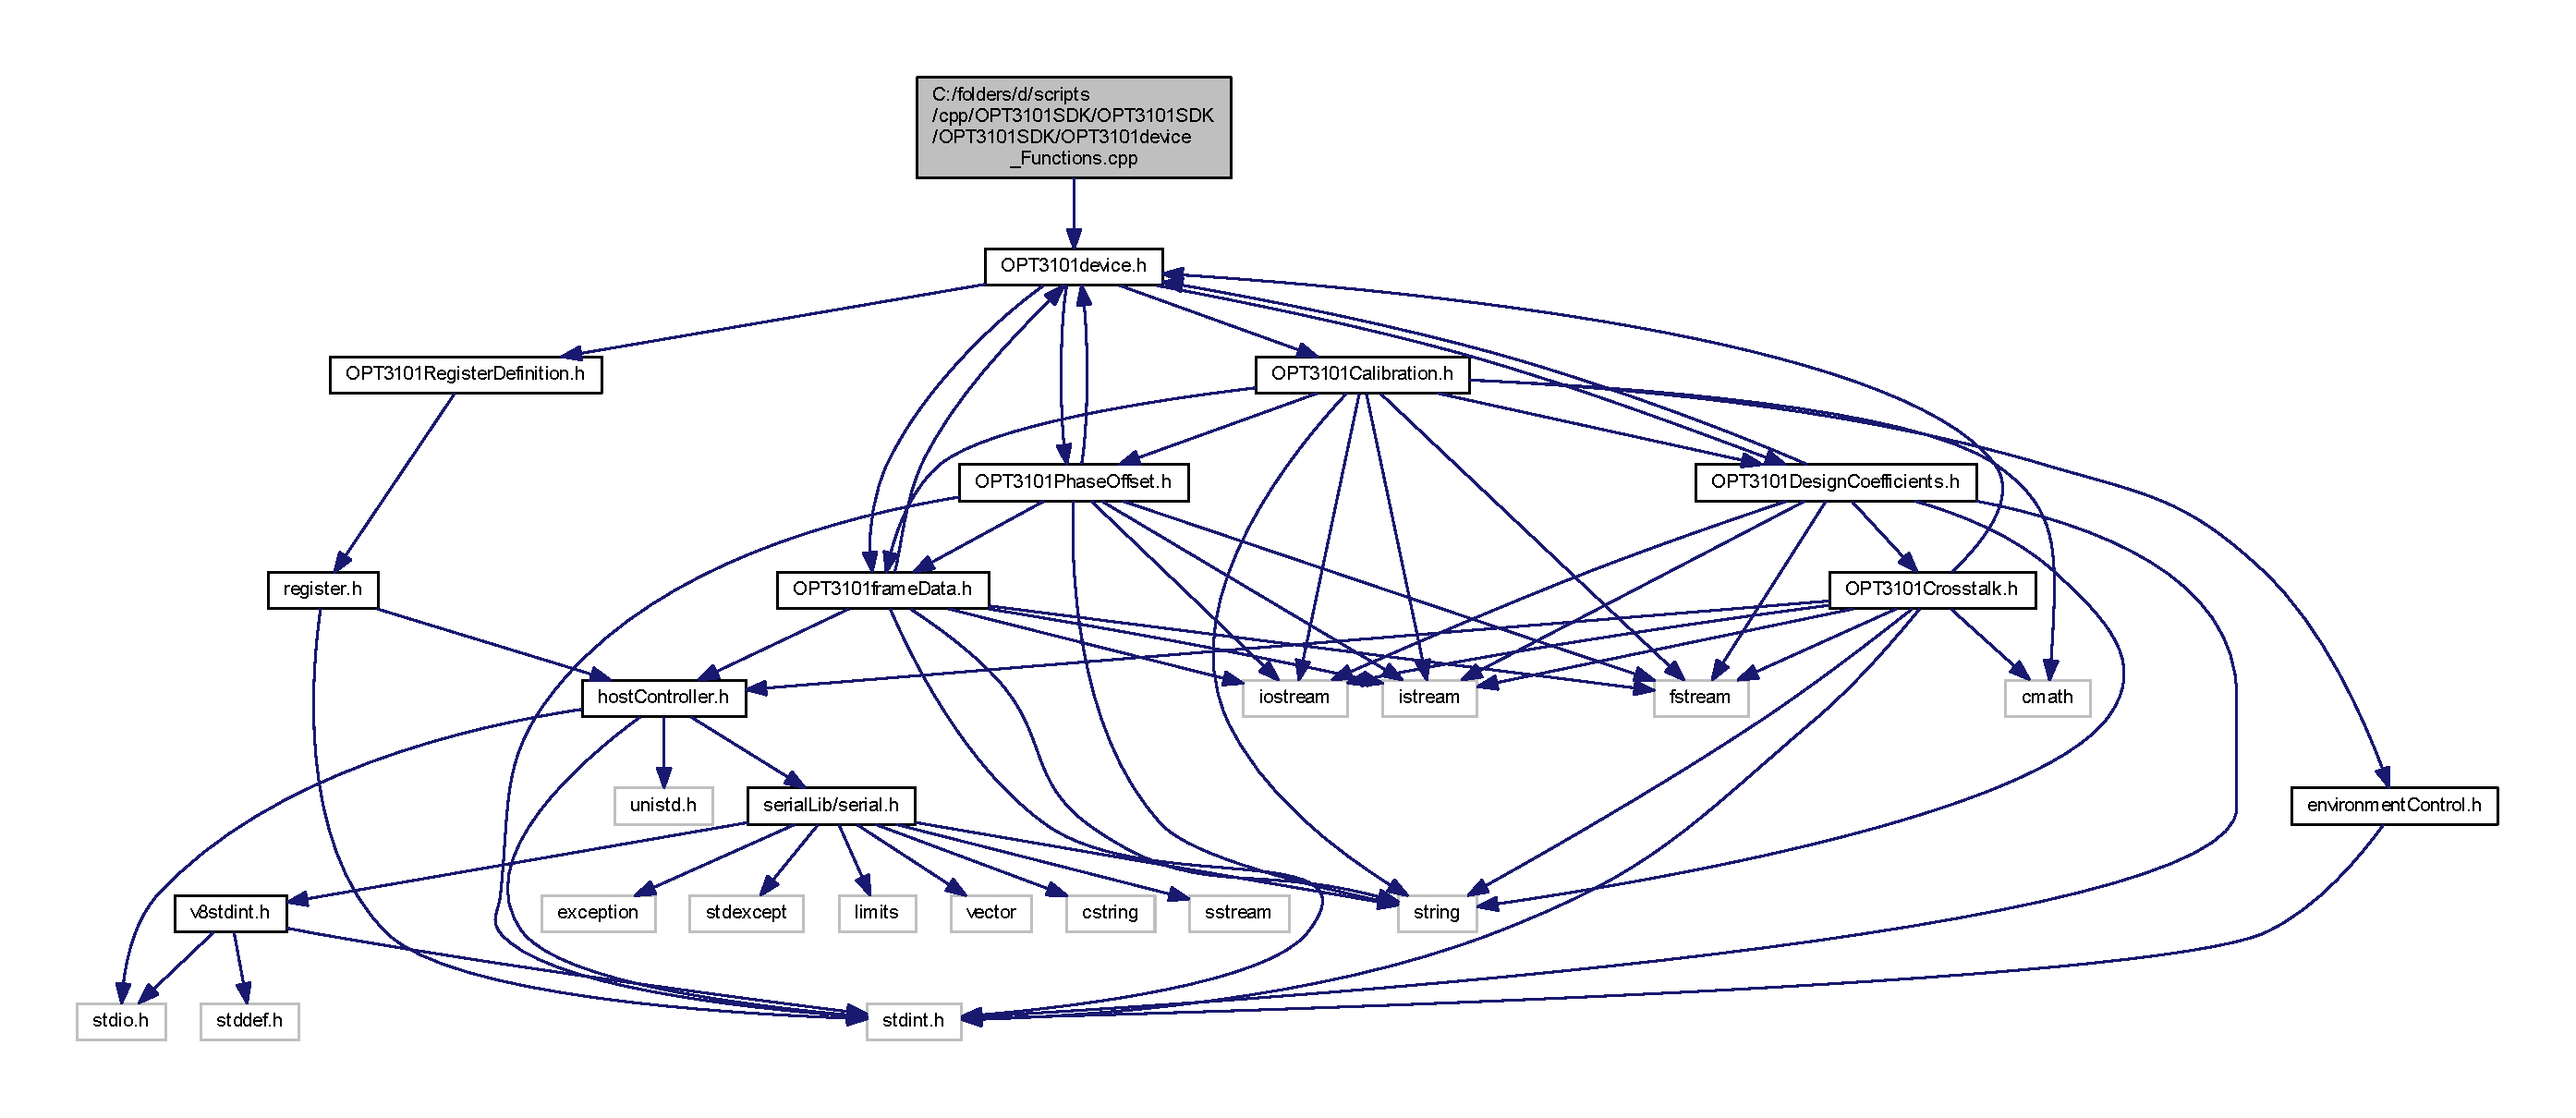
\includegraphics[width=350pt]{_o_p_t3101device___functions_8cpp__incl}
\end{center}
\end{figure}


\subsection{Detailed Description}
\begin{DoxyAuthor}{Author}
Karthik Rajagopal \href{mailto:krthik@ti.com}{\tt krthik@ti.\+com} 
\end{DoxyAuthor}
\begin{DoxyVersion}{Version}
0.\+8
\end{DoxyVersion}
\hypertarget{register_8h_COPYRIGHT}{}\subsection{C\+O\+P\+Y\+R\+I\+G\+HT}\label{register_8h_COPYRIGHT}
T\+E\+X\+AS I\+N\+S\+T\+R\+U\+M\+E\+N\+TS T\+E\+XT F\+I\+LE L\+I\+C\+E\+N\+SE Copyright (c) 2018 Texas Instruments Incorporated All rights reserved not granted herein. Limited License. Texas Instruments Incorporated grants a world-\/wide, royalty-\/free, non-\/exclusive license under copyrights and patents it now or hereafter owns or controls to make, have made, use, import, offer to sell and sell (\char`\"{}\+Utilize\char`\"{}) this software subject to the terms herein. With respect to the foregoing patent license, such license is granted solely to the extent that any such patent is necessary to Utilize the software alone. The patent license shall not apply to any combinations which include this software, other than combinations with devices manufactured by or for TI (�\+TI Devices�). No hardware patent is licensed hereunder. Redistributions must preserve existing copyright notices and reproduce this license (including the above copyright notice and the disclaimer and (if applicable) source code license limitations below) in the documentation and/or other materials provided with the distribution Redistribution and use in binary form, without modification, are permitted provided that the following conditions are met\+:
\begin{DoxyItemize}
\item No reverse engineering, decompilation, or disassembly of this software is permitted with respect to any software provided in binary form.
\item any redistribution and use are licensed by TI for use only with TI Devices.
\item Nothing shall obligate TI to provide you with source code for the software licensed and provided to you in object code. If software source code is provided to you, modification and redistribution of the source code are permitted provided that the following conditions are met\+:
\item any redistribution and use of the source code, including any resulting derivative works, are licensed by TI for use only with TI Devices.
\item any redistribution and use of any object code compiled from the source code and any resulting derivative works, are licensed by TI for use only with TI Devices. Neither the name of Texas Instruments Incorporated nor the names of its suppliers may be used to endorse or promote products derived from this software without specific prior written permission. D\+I\+S\+C\+L\+A\+I\+M\+ER. T\+H\+IS S\+O\+F\+T\+W\+A\+RE IS P\+R\+O\+V\+I\+D\+ED BY TI A\+ND T\+I�S L\+I\+C\+E\+N\+S\+O\+RS \char`\"{}\+A\+S I\+S\char`\"{} A\+ND A\+NY E\+X\+P\+R\+E\+SS OR I\+M\+P\+L\+I\+ED W\+A\+R\+R\+A\+N\+T\+I\+ES, I\+N\+C\+L\+U\+D\+I\+NG, B\+UT N\+OT L\+I\+M\+I\+T\+ED TO, T\+HE I\+M\+P\+L\+I\+ED W\+A\+R\+R\+A\+N\+T\+I\+ES OF M\+E\+R\+C\+H\+A\+N\+T\+A\+B\+I\+L\+I\+TY A\+ND F\+I\+T\+N\+E\+SS F\+OR A P\+A\+R\+T\+I\+C\+U\+L\+AR P\+U\+R\+P\+O\+SE A\+RE D\+I\+S\+C\+L\+A\+I\+M\+ED. IN NO E\+V\+E\+NT S\+H\+A\+LL TI A\+ND T\+I�S L\+I\+C\+E\+N\+S\+O\+RS BE L\+I\+A\+B\+LE F\+OR A\+NY D\+I\+R\+E\+CT, I\+N\+D\+I\+R\+E\+CT, I\+N\+C\+I\+D\+E\+N\+T\+AL, S\+P\+E\+C\+I\+AL, E\+X\+E\+M\+P\+L\+A\+RY, OR C\+O\+N\+S\+E\+Q\+U\+E\+N\+T\+I\+AL D\+A\+M\+A\+G\+ES (I\+N\+C\+L\+U\+D\+I\+NG, B\+UT N\+OT L\+I\+M\+I\+T\+ED TO, P\+R\+O\+C\+U\+R\+E\+M\+E\+NT OF S\+U\+B\+S\+T\+I\+T\+U\+TE G\+O\+O\+DS OR S\+E\+R\+V\+I\+C\+ES; L\+O\+SS OF U\+SE, D\+A\+TA, OR P\+R\+O\+F\+I\+TS; OR B\+U\+S\+I\+N\+E\+SS I\+N\+T\+E\+R\+R\+U\+P\+T\+I\+ON) H\+O\+W\+E\+V\+ER C\+A\+U\+S\+ED A\+ND ON A\+NY T\+H\+E\+O\+RY OF L\+I\+A\+B\+I\+L\+I\+TY, W\+H\+E\+T\+H\+ER IN C\+O\+N\+T\+R\+A\+CT, S\+T\+R\+I\+CT L\+I\+A\+B\+I\+L\+I\+TY, OR T\+O\+RT (I\+N\+C\+L\+U\+D\+I\+NG N\+E\+G\+L\+I\+G\+E\+N\+CE OR O\+T\+H\+E\+R\+W\+I\+SE) A\+R\+I\+S\+I\+NG IN A\+NY W\+AY O\+UT OF T\+HE U\+SE OF T\+H\+IS S\+O\+F\+T\+W\+A\+RE, E\+V\+EN IF A\+D\+V\+I\+S\+ED OF T\+HE P\+O\+S\+S\+I\+B\+I\+L\+I\+TY OF S\+U\+CH D\+A\+M\+A\+GE.
\end{DoxyItemize}\hypertarget{register_8h_DESCRIPTION}{}\subsection{D\+E\+S\+C\+R\+I\+P\+T\+I\+ON}\label{register_8h_DESCRIPTION}
The file contains methods definitions for classes \mbox{\hyperlink{class_o_p_t3101_1_1device}{O\+P\+T3101\+::device}} \mbox{\hyperlink{class_o_p_t3101_1_1frame_data}{O\+P\+T3101\+::frame\+Data}} \mbox{\hyperlink{class_o_p_t3101_1_1calibration_c}{O\+P\+T3101\+::calibrationC}} 
\hypertarget{_o_p_t3101device___register_map_8cpp}{}\section{C\+:/folders/d/scripts/cpp/\+O\+P\+T3101\+S\+D\+K/\+O\+P\+T3101\+S\+D\+K/\+O\+P\+T3101\+S\+D\+K/\+O\+P\+T3101device\+\_\+\+Register\+Map.cpp File Reference}
\label{_o_p_t3101device___register_map_8cpp}\index{C\+:/folders/d/scripts/cpp/\+O\+P\+T3101\+S\+D\+K/\+O\+P\+T3101\+S\+D\+K/\+O\+P\+T3101\+S\+D\+K/\+O\+P\+T3101device\+\_\+\+Register\+Map.\+cpp@{C\+:/folders/d/scripts/cpp/\+O\+P\+T3101\+S\+D\+K/\+O\+P\+T3101\+S\+D\+K/\+O\+P\+T3101\+S\+D\+K/\+O\+P\+T3101device\+\_\+\+Register\+Map.\+cpp}}
{\ttfamily \#include \char`\"{}O\+P\+T3101\+Register\+Definition.\+h\char`\"{}}\newline
Include dependency graph for O\+P\+T3101device\+\_\+\+Register\+Map.\+cpp\+:\nopagebreak
\begin{figure}[H]
\begin{center}
\leavevmode
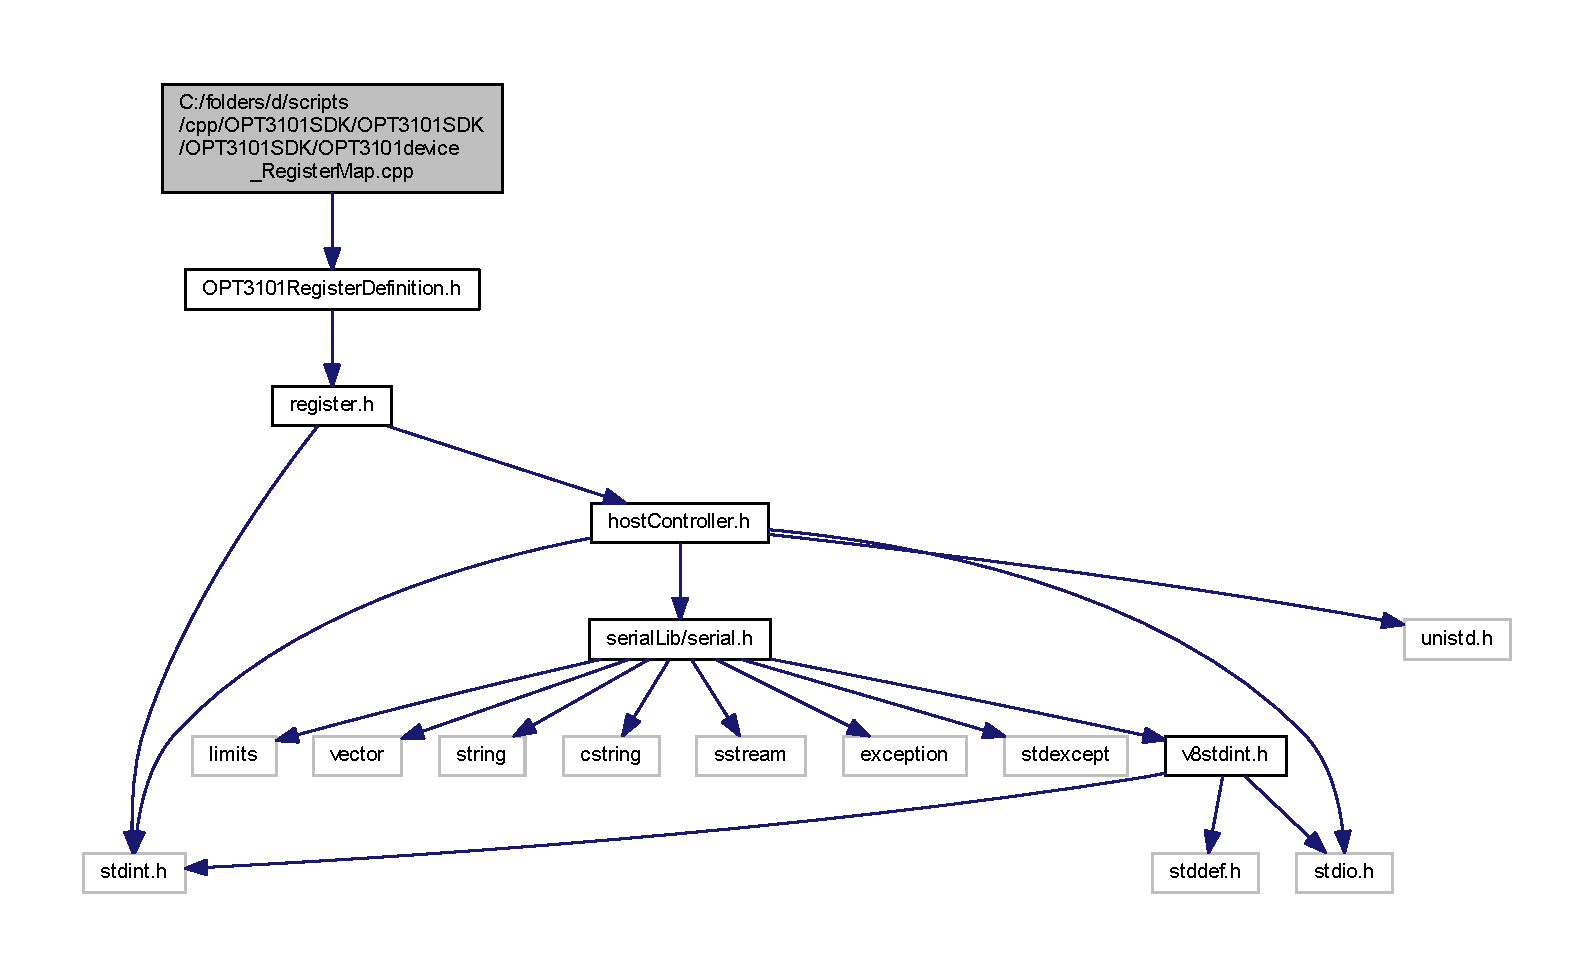
\includegraphics[width=350pt]{_o_p_t3101device___register_map_8cpp__incl}
\end{center}
\end{figure}


\subsection{Detailed Description}
\begin{DoxyAuthor}{Author}
Karthik Rajagopal \href{mailto:krthik@ti.com}{\tt krthik@ti.\+com} 
\end{DoxyAuthor}
\begin{DoxyVersion}{Version}
0.\+8
\end{DoxyVersion}
\hypertarget{register_8h_COPYRIGHT}{}\subsection{C\+O\+P\+Y\+R\+I\+G\+HT}\label{register_8h_COPYRIGHT}
T\+E\+X\+AS I\+N\+S\+T\+R\+U\+M\+E\+N\+TS T\+E\+XT F\+I\+LE L\+I\+C\+E\+N\+SE Copyright (c) 2018 Texas Instruments Incorporated All rights reserved not granted herein. Limited License. Texas Instruments Incorporated grants a world-\/wide, royalty-\/free, non-\/exclusive license under copyrights and patents it now or hereafter owns or controls to make, have made, use, import, offer to sell and sell (\char`\"{}\+Utilize\char`\"{}) this software subject to the terms herein. With respect to the foregoing patent license, such license is granted solely to the extent that any such patent is necessary to Utilize the software alone. The patent license shall not apply to any combinations which include this software, other than combinations with devices manufactured by or for TI (“\+TI Devices”). No hardware patent is licensed hereunder. Redistributions must preserve existing copyright notices and reproduce this license (including the above copyright notice and the disclaimer and (if applicable) source code license limitations below) in the documentation and/or other materials provided with the distribution Redistribution and use in binary form, without modification, are permitted provided that the following conditions are met\+:
\begin{DoxyItemize}
\item No reverse engineering, decompilation, or disassembly of this software is permitted with respect to any software provided in binary form.
\item any redistribution and use are licensed by TI for use only with TI Devices.
\item Nothing shall obligate TI to provide you with source code for the software licensed and provided to you in object code. If software source code is provided to you, modification and redistribution of the source code are permitted provided that the following conditions are met\+:
\item any redistribution and use of the source code, including any resulting derivative works, are licensed by TI for use only with TI Devices.
\item any redistribution and use of any object code compiled from the source code and any resulting derivative works, are licensed by TI for use only with TI Devices. Neither the name of Texas Instruments Incorporated nor the names of its suppliers may be used to endorse or promote products derived from this software without specific prior written permission. D\+I\+S\+C\+L\+A\+I\+M\+ER. T\+H\+IS S\+O\+F\+T\+W\+A\+RE IS P\+R\+O\+V\+I\+D\+ED BY TI A\+ND T\+I’S L\+I\+C\+E\+N\+S\+O\+RS \char`\"{}\+A\+S I\+S\char`\"{} A\+ND A\+NY E\+X\+P\+R\+E\+SS OR I\+M\+P\+L\+I\+ED W\+A\+R\+R\+A\+N\+T\+I\+ES, I\+N\+C\+L\+U\+D\+I\+NG, B\+UT N\+OT L\+I\+M\+I\+T\+ED TO, T\+HE I\+M\+P\+L\+I\+ED W\+A\+R\+R\+A\+N\+T\+I\+ES OF M\+E\+R\+C\+H\+A\+N\+T\+A\+B\+I\+L\+I\+TY A\+ND F\+I\+T\+N\+E\+SS F\+OR A P\+A\+R\+T\+I\+C\+U\+L\+AR P\+U\+R\+P\+O\+SE A\+RE D\+I\+S\+C\+L\+A\+I\+M\+ED. IN NO E\+V\+E\+NT S\+H\+A\+LL TI A\+ND T\+I’S L\+I\+C\+E\+N\+S\+O\+RS BE L\+I\+A\+B\+LE F\+OR A\+NY D\+I\+R\+E\+CT, I\+N\+D\+I\+R\+E\+CT, I\+N\+C\+I\+D\+E\+N\+T\+AL, S\+P\+E\+C\+I\+AL, E\+X\+E\+M\+P\+L\+A\+RY, OR C\+O\+N\+S\+E\+Q\+U\+E\+N\+T\+I\+AL D\+A\+M\+A\+G\+ES (I\+N\+C\+L\+U\+D\+I\+NG, B\+UT N\+OT L\+I\+M\+I\+T\+ED TO, P\+R\+O\+C\+U\+R\+E\+M\+E\+NT OF S\+U\+B\+S\+T\+I\+T\+U\+TE G\+O\+O\+DS OR S\+E\+R\+V\+I\+C\+ES; L\+O\+SS OF U\+SE, D\+A\+TA, OR P\+R\+O\+F\+I\+TS; OR B\+U\+S\+I\+N\+E\+SS I\+N\+T\+E\+R\+R\+U\+P\+T\+I\+ON) H\+O\+W\+E\+V\+ER C\+A\+U\+S\+ED A\+ND ON A\+NY T\+H\+E\+O\+RY OF L\+I\+A\+B\+I\+L\+I\+TY, W\+H\+E\+T\+H\+ER IN C\+O\+N\+T\+R\+A\+CT, S\+T\+R\+I\+CT L\+I\+A\+B\+I\+L\+I\+TY, OR T\+O\+RT (I\+N\+C\+L\+U\+D\+I\+NG N\+E\+G\+L\+I\+G\+E\+N\+CE OR O\+T\+H\+E\+R\+W\+I\+SE) A\+R\+I\+S\+I\+NG IN A\+NY W\+AY O\+UT OF T\+HE U\+SE OF T\+H\+IS S\+O\+F\+T\+W\+A\+RE, E\+V\+EN IF A\+D\+V\+I\+S\+ED OF T\+HE P\+O\+S\+S\+I\+B\+I\+L\+I\+TY OF S\+U\+CH D\+A\+M\+A\+GE.
\end{DoxyItemize}\hypertarget{register_8h_DESCRIPTION}{}\subsection{D\+E\+S\+C\+R\+I\+P\+T\+I\+ON}\label{register_8h_DESCRIPTION}
The file contains \mbox{\hyperlink{class_o_p_t3101_1_1registers}{O\+P\+T3101\+::registers}} class constructor and assignment 
\hypertarget{_o_p_t3101frame_data_8h}{}\section{C\+:/folders/d/scripts/cpp/\+O\+P\+T3101\+S\+D\+K/\+O\+P\+T3101\+S\+D\+K/\+O\+P\+T3101\+S\+D\+K/\+O\+P\+T3101frame\+Data.h File Reference}
\label{_o_p_t3101frame_data_8h}\index{C\+:/folders/d/scripts/cpp/\+O\+P\+T3101\+S\+D\+K/\+O\+P\+T3101\+S\+D\+K/\+O\+P\+T3101\+S\+D\+K/\+O\+P\+T3101frame\+Data.\+h@{C\+:/folders/d/scripts/cpp/\+O\+P\+T3101\+S\+D\+K/\+O\+P\+T3101\+S\+D\+K/\+O\+P\+T3101\+S\+D\+K/\+O\+P\+T3101frame\+Data.\+h}}
{\ttfamily \#include $<$stdint.\+h$>$}\newline
{\ttfamily \#include \char`\"{}host\+Controller.\+h\char`\"{}}\newline
{\ttfamily \#include \char`\"{}O\+P\+T3101device.\+h\char`\"{}}\newline
{\ttfamily \#include $<$fstream$>$}\newline
{\ttfamily \#include $<$iostream$>$}\newline
{\ttfamily \#include $<$istream$>$}\newline
{\ttfamily \#include $<$string$>$}\newline
Include dependency graph for O\+P\+T3101frame\+Data.\+h\+:\nopagebreak
\begin{figure}[H]
\begin{center}
\leavevmode
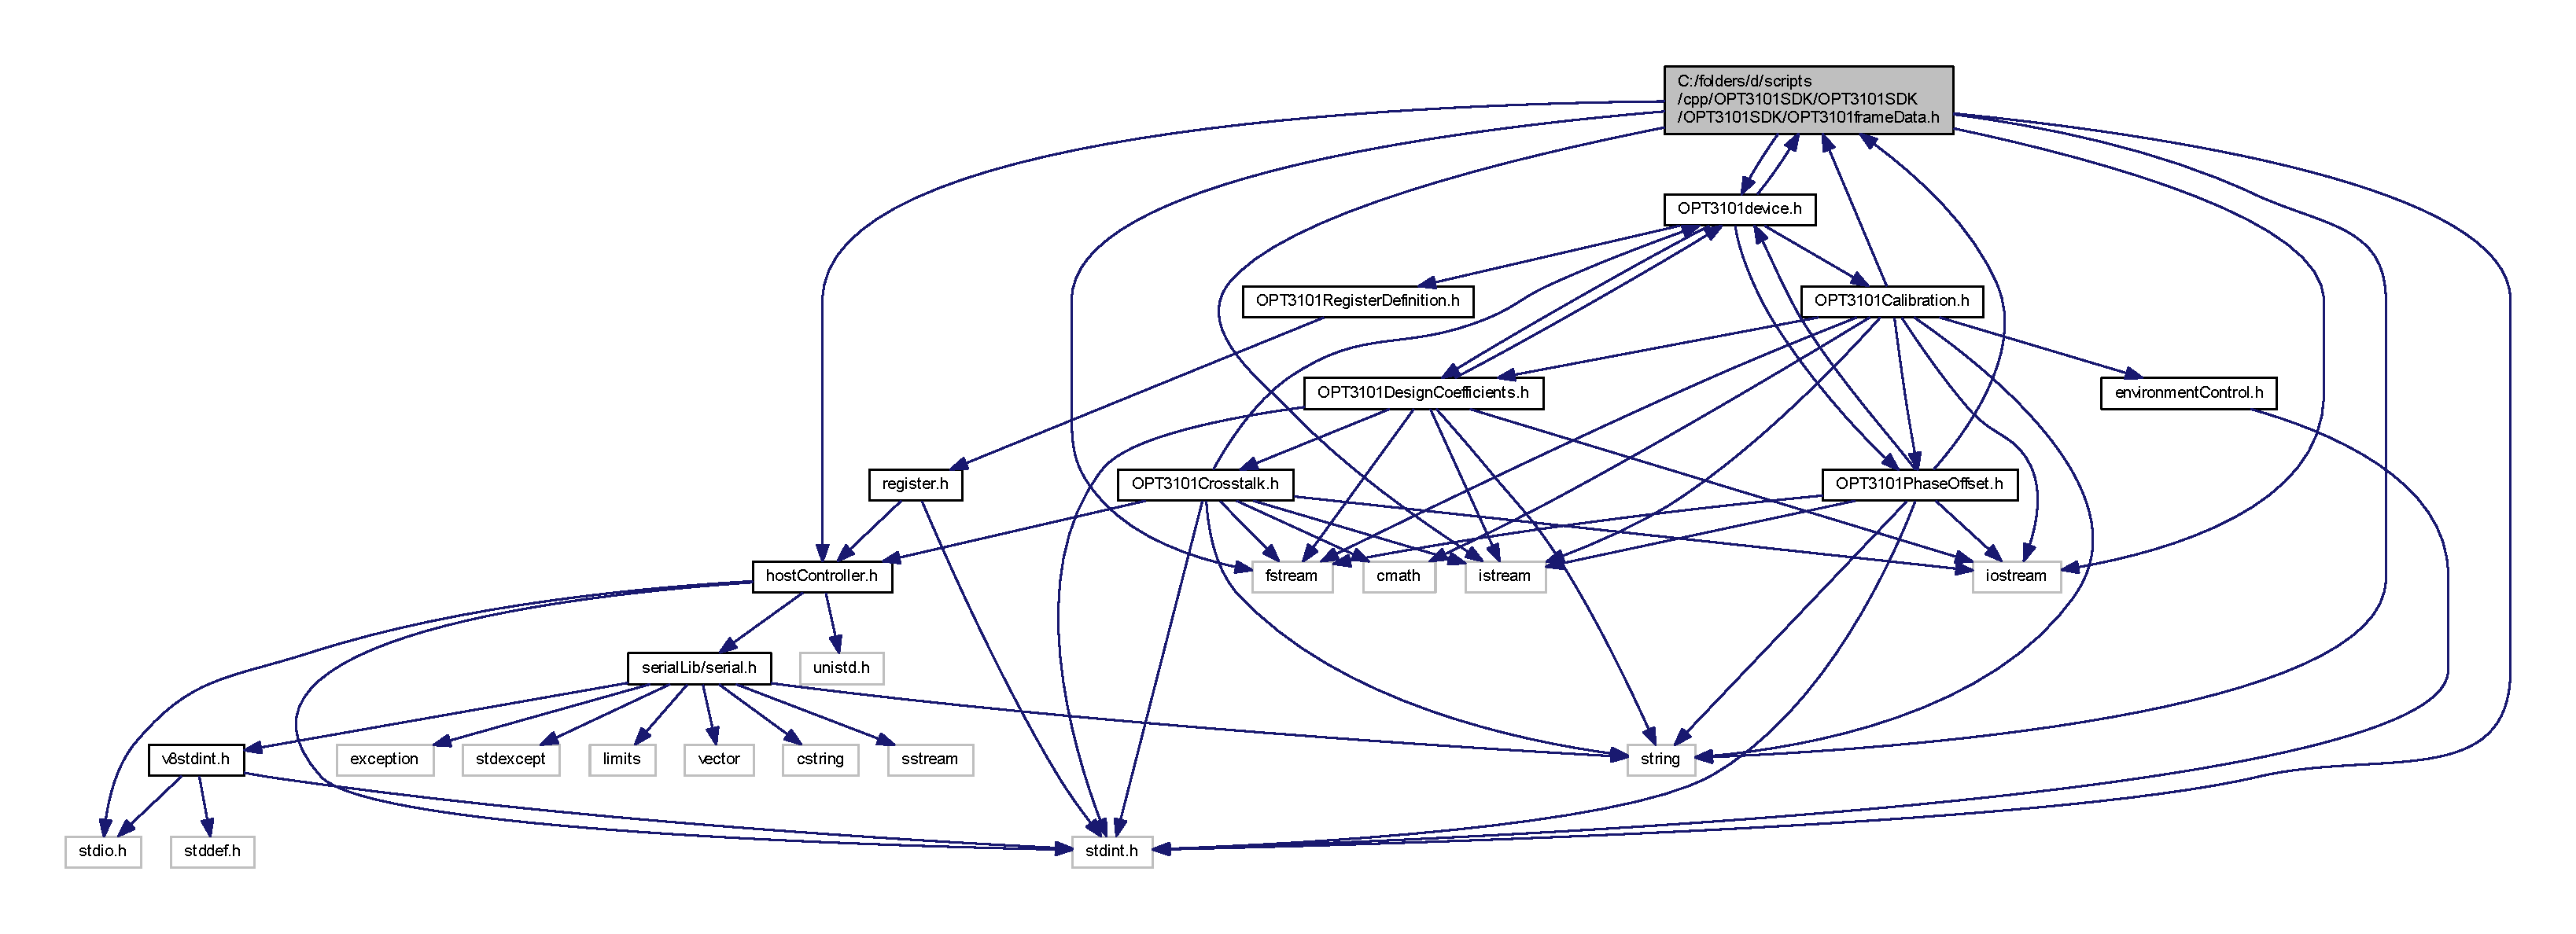
\includegraphics[width=350pt]{_o_p_t3101frame_data_8h__incl}
\end{center}
\end{figure}
This graph shows which files directly or indirectly include this file\+:\nopagebreak
\begin{figure}[H]
\begin{center}
\leavevmode
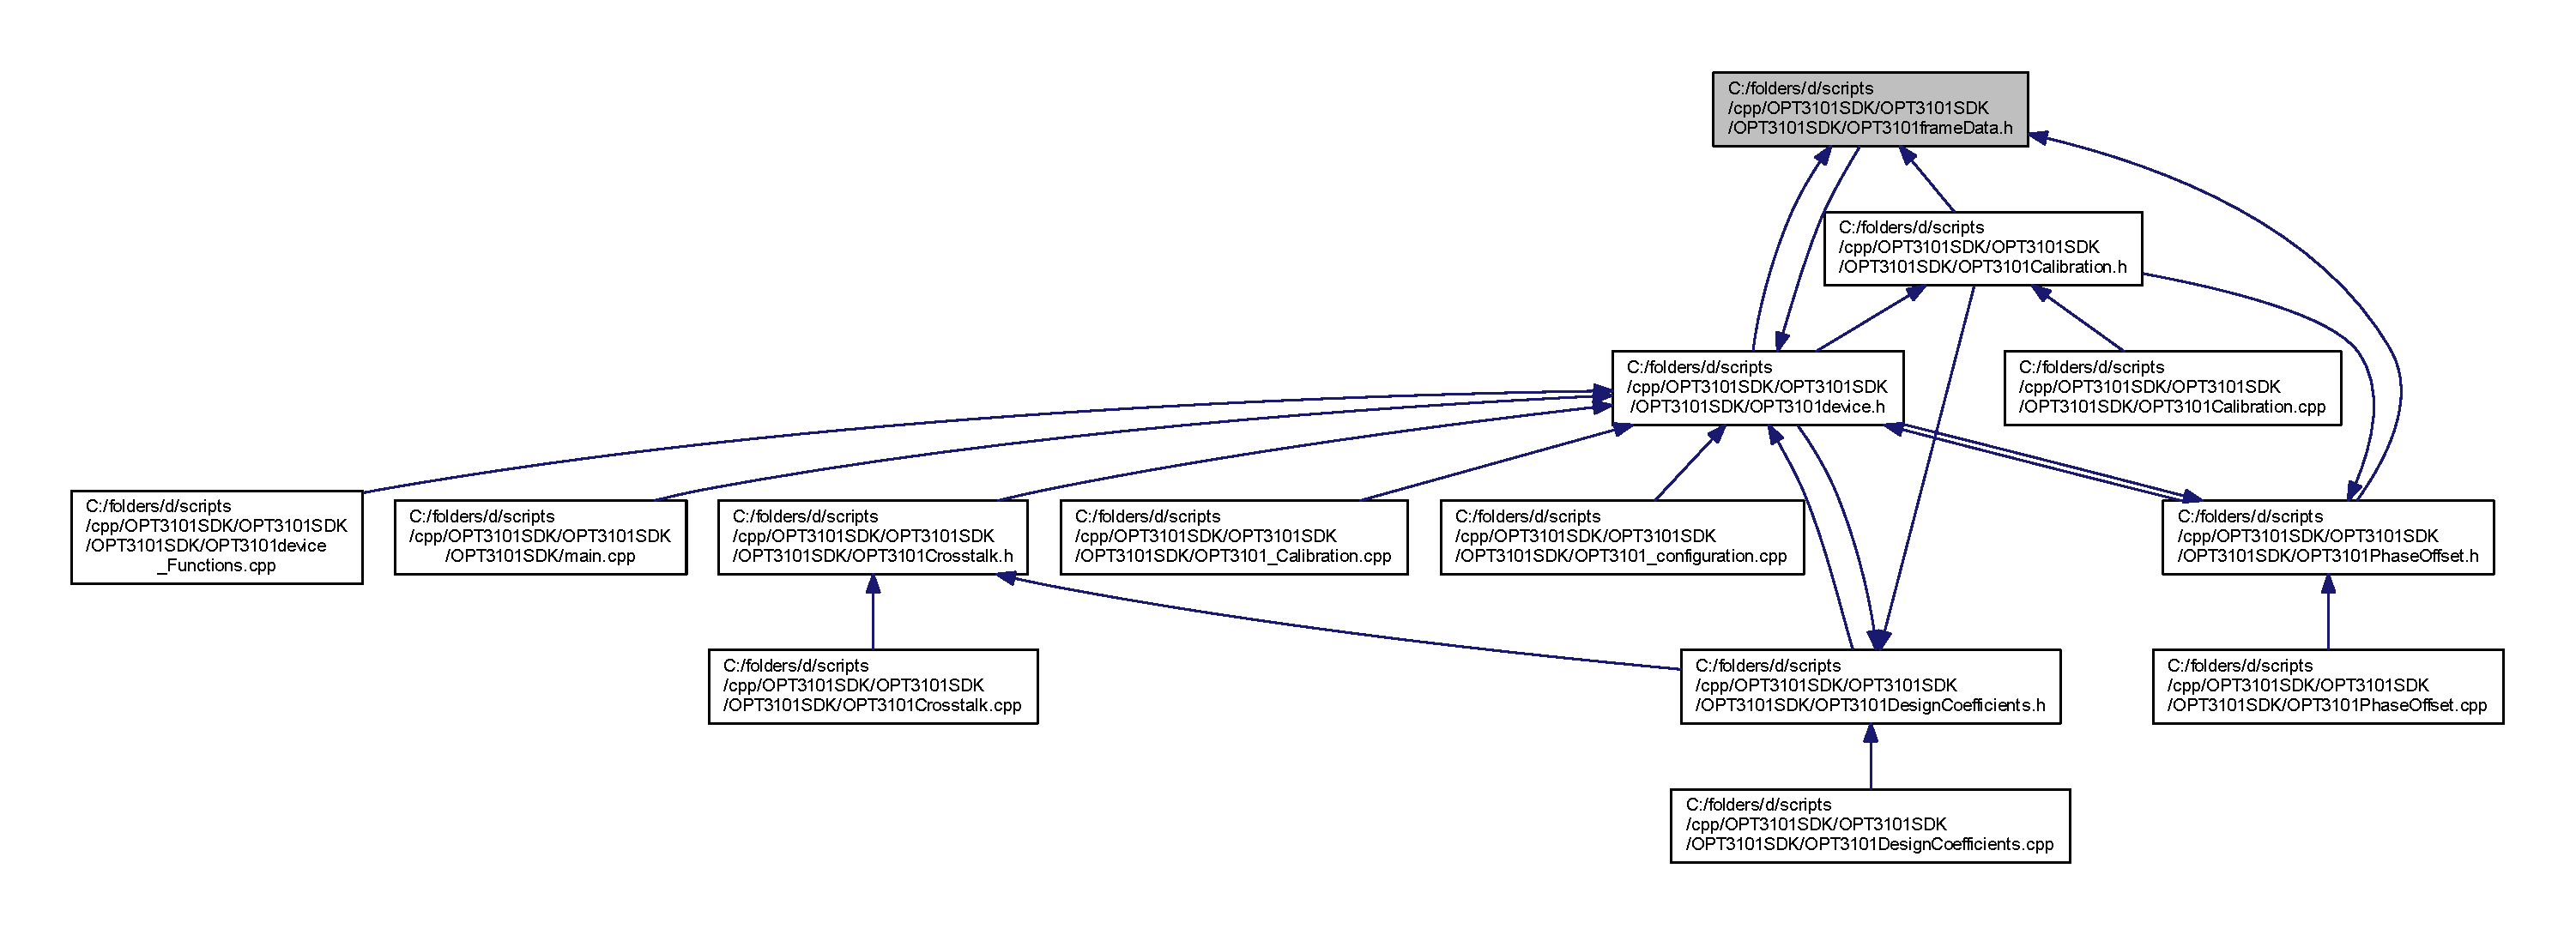
\includegraphics[width=350pt]{_o_p_t3101frame_data_8h__dep__incl}
\end{center}
\end{figure}
\subsection*{Classes}
\begin{DoxyCompactItemize}
\item 
class \mbox{\hyperlink{class_o_p_t3101_1_1frame_data}{O\+P\+T3101\+::frame\+Data}}
\begin{DoxyCompactList}\small\item\em Class the data output from \mbox{\hyperlink{namespace_o_p_t3101}{O\+P\+T3101}} device. \end{DoxyCompactList}\end{DoxyCompactItemize}
\subsection*{Namespaces}
\begin{DoxyCompactItemize}
\item 
 \mbox{\hyperlink{namespace_o_p_t3101}{O\+P\+T3101}}
\begin{DoxyCompactList}\small\item\em \mbox{\hyperlink{class_o_p_t3101_1_1device}{O\+P\+T3101\+::device}} declaration This is declared here to avoid cyclic reference of classes. \end{DoxyCompactList}\end{DoxyCompactItemize}


\subsection{Detailed Description}
\begin{DoxyAuthor}{Author}
Karthik Rajagopal \href{mailto:krthik@ti.com}{\tt krthik@ti.\+com} 
\end{DoxyAuthor}
\begin{DoxyVersion}{Version}
0.\+8
\end{DoxyVersion}
\hypertarget{register_8h_COPYRIGHT}{}\subsection{C\+O\+P\+Y\+R\+I\+G\+HT}\label{register_8h_COPYRIGHT}
T\+E\+X\+AS I\+N\+S\+T\+R\+U\+M\+E\+N\+TS T\+E\+XT F\+I\+LE L\+I\+C\+E\+N\+SE Copyright (c) 2018 Texas Instruments Incorporated All rights reserved not granted herein. Limited License. Texas Instruments Incorporated grants a world-\/wide, royalty-\/free, non-\/exclusive license under copyrights and patents it now or hereafter owns or controls to make, have made, use, import, offer to sell and sell (\char`\"{}\+Utilize\char`\"{}) this software subject to the terms herein. With respect to the foregoing patent license, such license is granted solely to the extent that any such patent is necessary to Utilize the software alone. The patent license shall not apply to any combinations which include this software, other than combinations with devices manufactured by or for TI (�\+TI Devices�). No hardware patent is licensed hereunder. Redistributions must preserve existing copyright notices and reproduce this license (including the above copyright notice and the disclaimer and (if applicable) source code license limitations below) in the documentation and/or other materials provided with the distribution Redistribution and use in binary form, without modification, are permitted provided that the following conditions are met\+:
\begin{DoxyItemize}
\item No reverse engineering, decompilation, or disassembly of this software is permitted with respect to any software provided in binary form.
\item any redistribution and use are licensed by TI for use only with TI Devices.
\item Nothing shall obligate TI to provide you with source code for the software licensed and provided to you in object code. If software source code is provided to you, modification and redistribution of the source code are permitted provided that the following conditions are met\+:
\item any redistribution and use of the source code, including any resulting derivative works, are licensed by TI for use only with TI Devices.
\item any redistribution and use of any object code compiled from the source code and any resulting derivative works, are licensed by TI for use only with TI Devices. Neither the name of Texas Instruments Incorporated nor the names of its suppliers may be used to endorse or promote products derived from this software without specific prior written permission. D\+I\+S\+C\+L\+A\+I\+M\+ER. T\+H\+IS S\+O\+F\+T\+W\+A\+RE IS P\+R\+O\+V\+I\+D\+ED BY TI A\+ND T\+I�S L\+I\+C\+E\+N\+S\+O\+RS \char`\"{}\+A\+S I\+S\char`\"{} A\+ND A\+NY E\+X\+P\+R\+E\+SS OR I\+M\+P\+L\+I\+ED W\+A\+R\+R\+A\+N\+T\+I\+ES, I\+N\+C\+L\+U\+D\+I\+NG, B\+UT N\+OT L\+I\+M\+I\+T\+ED TO, T\+HE I\+M\+P\+L\+I\+ED W\+A\+R\+R\+A\+N\+T\+I\+ES OF M\+E\+R\+C\+H\+A\+N\+T\+A\+B\+I\+L\+I\+TY A\+ND F\+I\+T\+N\+E\+SS F\+OR A P\+A\+R\+T\+I\+C\+U\+L\+AR P\+U\+R\+P\+O\+SE A\+RE D\+I\+S\+C\+L\+A\+I\+M\+ED. IN NO E\+V\+E\+NT S\+H\+A\+LL TI A\+ND T\+I�S L\+I\+C\+E\+N\+S\+O\+RS BE L\+I\+A\+B\+LE F\+OR A\+NY D\+I\+R\+E\+CT, I\+N\+D\+I\+R\+E\+CT, I\+N\+C\+I\+D\+E\+N\+T\+AL, S\+P\+E\+C\+I\+AL, E\+X\+E\+M\+P\+L\+A\+RY, OR C\+O\+N\+S\+E\+Q\+U\+E\+N\+T\+I\+AL D\+A\+M\+A\+G\+ES (I\+N\+C\+L\+U\+D\+I\+NG, B\+UT N\+OT L\+I\+M\+I\+T\+ED TO, P\+R\+O\+C\+U\+R\+E\+M\+E\+NT OF S\+U\+B\+S\+T\+I\+T\+U\+TE G\+O\+O\+DS OR S\+E\+R\+V\+I\+C\+ES; L\+O\+SS OF U\+SE, D\+A\+TA, OR P\+R\+O\+F\+I\+TS; OR B\+U\+S\+I\+N\+E\+SS I\+N\+T\+E\+R\+R\+U\+P\+T\+I\+ON) H\+O\+W\+E\+V\+ER C\+A\+U\+S\+ED A\+ND ON A\+NY T\+H\+E\+O\+RY OF L\+I\+A\+B\+I\+L\+I\+TY, W\+H\+E\+T\+H\+ER IN C\+O\+N\+T\+R\+A\+CT, S\+T\+R\+I\+CT L\+I\+A\+B\+I\+L\+I\+TY, OR T\+O\+RT (I\+N\+C\+L\+U\+D\+I\+NG N\+E\+G\+L\+I\+G\+E\+N\+CE OR O\+T\+H\+E\+R\+W\+I\+SE) A\+R\+I\+S\+I\+NG IN A\+NY W\+AY O\+UT OF T\+HE U\+SE OF T\+H\+IS S\+O\+F\+T\+W\+A\+RE, E\+V\+EN IF A\+D\+V\+I\+S\+ED OF T\+HE P\+O\+S\+S\+I\+B\+I\+L\+I\+TY OF S\+U\+CH D\+A\+M\+A\+GE.
\end{DoxyItemize}\hypertarget{register_8h_DESCRIPTION}{}\subsection{D\+E\+S\+C\+R\+I\+P\+T\+I\+ON}\label{register_8h_DESCRIPTION}
This file contains the \mbox{\hyperlink{class_o_p_t3101_1_1frame_data}{O\+P\+T3101\+::frame\+Data}} class declaraction 
\hypertarget{_o_p_t3101_phase_offset_8cpp}{}\section{C\+:/folders/d/scripts/cpp/\+O\+P\+T3101\+S\+D\+K/\+O\+P\+T3101\+S\+D\+K/\+O\+P\+T3101\+S\+D\+K/\+O\+P\+T3101\+Phase\+Offset.cpp File Reference}
\label{_o_p_t3101_phase_offset_8cpp}\index{C\+:/folders/d/scripts/cpp/\+O\+P\+T3101\+S\+D\+K/\+O\+P\+T3101\+S\+D\+K/\+O\+P\+T3101\+S\+D\+K/\+O\+P\+T3101\+Phase\+Offset.\+cpp@{C\+:/folders/d/scripts/cpp/\+O\+P\+T3101\+S\+D\+K/\+O\+P\+T3101\+S\+D\+K/\+O\+P\+T3101\+S\+D\+K/\+O\+P\+T3101\+Phase\+Offset.\+cpp}}
{\ttfamily \#include \char`\"{}O\+P\+T3101\+Phase\+Offset.\+h\char`\"{}}\newline
Include dependency graph for O\+P\+T3101\+Phase\+Offset.\+cpp\+:\nopagebreak
\begin{figure}[H]
\begin{center}
\leavevmode
\includegraphics[width=350pt]{_o_p_t3101_phase_offset_8cpp__incl}
\end{center}
\end{figure}


\subsection{Detailed Description}
\begin{DoxyAuthor}{Author}
Karthik Rajagopal \href{mailto:krthik@ti.com}{\tt krthik@ti.\+com} 
\end{DoxyAuthor}
\begin{DoxyVersion}{Version}
0.\+8
\end{DoxyVersion}
\hypertarget{register_8h_COPYRIGHT}{}\subsection{C\+O\+P\+Y\+R\+I\+G\+HT}\label{register_8h_COPYRIGHT}
T\+E\+X\+AS I\+N\+S\+T\+R\+U\+M\+E\+N\+TS T\+E\+XT F\+I\+LE L\+I\+C\+E\+N\+SE Copyright (c) 2018 Texas Instruments Incorporated All rights reserved not granted herein. Limited License. Texas Instruments Incorporated grants a world-\/wide, royalty-\/free, non-\/exclusive license under copyrights and patents it now or hereafter owns or controls to make, have made, use, import, offer to sell and sell (\char`\"{}\+Utilize\char`\"{}) this software subject to the terms herein. With respect to the foregoing patent license, such license is granted solely to the extent that any such patent is necessary to Utilize the software alone. The patent license shall not apply to any combinations which include this software, other than combinations with devices manufactured by or for TI (�\+TI Devices�). No hardware patent is licensed hereunder. Redistributions must preserve existing copyright notices and reproduce this license (including the above copyright notice and the disclaimer and (if applicable) source code license limitations below) in the documentation and/or other materials provided with the distribution Redistribution and use in binary form, without modification, are permitted provided that the following conditions are met\+:
\begin{DoxyItemize}
\item No reverse engineering, decompilation, or disassembly of this software is permitted with respect to any software provided in binary form.
\item any redistribution and use are licensed by TI for use only with TI Devices.
\item Nothing shall obligate TI to provide you with source code for the software licensed and provided to you in object code. If software source code is provided to you, modification and redistribution of the source code are permitted provided that the following conditions are met\+:
\item any redistribution and use of the source code, including any resulting derivative works, are licensed by TI for use only with TI Devices.
\item any redistribution and use of any object code compiled from the source code and any resulting derivative works, are licensed by TI for use only with TI Devices. Neither the name of Texas Instruments Incorporated nor the names of its suppliers may be used to endorse or promote products derived from this software without specific prior written permission. D\+I\+S\+C\+L\+A\+I\+M\+ER. T\+H\+IS S\+O\+F\+T\+W\+A\+RE IS P\+R\+O\+V\+I\+D\+ED BY TI A\+ND T\+I�S L\+I\+C\+E\+N\+S\+O\+RS \char`\"{}\+A\+S I\+S\char`\"{} A\+ND A\+NY E\+X\+P\+R\+E\+SS OR I\+M\+P\+L\+I\+ED W\+A\+R\+R\+A\+N\+T\+I\+ES, I\+N\+C\+L\+U\+D\+I\+NG, B\+UT N\+OT L\+I\+M\+I\+T\+ED TO, T\+HE I\+M\+P\+L\+I\+ED W\+A\+R\+R\+A\+N\+T\+I\+ES OF M\+E\+R\+C\+H\+A\+N\+T\+A\+B\+I\+L\+I\+TY A\+ND F\+I\+T\+N\+E\+SS F\+OR A P\+A\+R\+T\+I\+C\+U\+L\+AR P\+U\+R\+P\+O\+SE A\+RE D\+I\+S\+C\+L\+A\+I\+M\+ED. IN NO E\+V\+E\+NT S\+H\+A\+LL TI A\+ND T\+I�S L\+I\+C\+E\+N\+S\+O\+RS BE L\+I\+A\+B\+LE F\+OR A\+NY D\+I\+R\+E\+CT, I\+N\+D\+I\+R\+E\+CT, I\+N\+C\+I\+D\+E\+N\+T\+AL, S\+P\+E\+C\+I\+AL, E\+X\+E\+M\+P\+L\+A\+RY, OR C\+O\+N\+S\+E\+Q\+U\+E\+N\+T\+I\+AL D\+A\+M\+A\+G\+ES (I\+N\+C\+L\+U\+D\+I\+NG, B\+UT N\+OT L\+I\+M\+I\+T\+ED TO, P\+R\+O\+C\+U\+R\+E\+M\+E\+NT OF S\+U\+B\+S\+T\+I\+T\+U\+TE G\+O\+O\+DS OR S\+E\+R\+V\+I\+C\+ES; L\+O\+SS OF U\+SE, D\+A\+TA, OR P\+R\+O\+F\+I\+TS; OR B\+U\+S\+I\+N\+E\+SS I\+N\+T\+E\+R\+R\+U\+P\+T\+I\+ON) H\+O\+W\+E\+V\+ER C\+A\+U\+S\+ED A\+ND ON A\+NY T\+H\+E\+O\+RY OF L\+I\+A\+B\+I\+L\+I\+TY, W\+H\+E\+T\+H\+ER IN C\+O\+N\+T\+R\+A\+CT, S\+T\+R\+I\+CT L\+I\+A\+B\+I\+L\+I\+TY, OR T\+O\+RT (I\+N\+C\+L\+U\+D\+I\+NG N\+E\+G\+L\+I\+G\+E\+N\+CE OR O\+T\+H\+E\+R\+W\+I\+SE) A\+R\+I\+S\+I\+NG IN A\+NY W\+AY O\+UT OF T\+HE U\+SE OF T\+H\+IS S\+O\+F\+T\+W\+A\+RE, E\+V\+EN IF A\+D\+V\+I\+S\+ED OF T\+HE P\+O\+S\+S\+I\+B\+I\+L\+I\+TY OF S\+U\+CH D\+A\+M\+A\+GE.
\end{DoxyItemize}\hypertarget{register_8h_DESCRIPTION}{}\subsection{D\+E\+S\+C\+R\+I\+P\+T\+I\+ON}\label{register_8h_DESCRIPTION}
This file contains the method definitions for class \mbox{\hyperlink{class_o_p_t3101_1_1phase_offset_c}{O\+P\+T3101\+::phase\+OffsetC}} 
\hypertarget{_o_p_t3101_phase_offset_8h}{}\section{C\+:/folders/d/scripts/cpp/\+O\+P\+T3101\+S\+D\+K/\+O\+P\+T3101\+S\+D\+K/\+O\+P\+T3101\+S\+D\+K/\+O\+P\+T3101\+Phase\+Offset.h File Reference}
\label{_o_p_t3101_phase_offset_8h}\index{C\+:/folders/d/scripts/cpp/\+O\+P\+T3101\+S\+D\+K/\+O\+P\+T3101\+S\+D\+K/\+O\+P\+T3101\+S\+D\+K/\+O\+P\+T3101\+Phase\+Offset.\+h@{C\+:/folders/d/scripts/cpp/\+O\+P\+T3101\+S\+D\+K/\+O\+P\+T3101\+S\+D\+K/\+O\+P\+T3101\+S\+D\+K/\+O\+P\+T3101\+Phase\+Offset.\+h}}
{\ttfamily \#include $<$stdint.\+h$>$}\newline
{\ttfamily \#include \char`\"{}O\+P\+T3101device.\+h\char`\"{}}\newline
{\ttfamily \#include \char`\"{}O\+P\+T3101frame\+Data.\+h\char`\"{}}\newline
{\ttfamily \#include $<$fstream$>$}\newline
{\ttfamily \#include $<$iostream$>$}\newline
{\ttfamily \#include $<$istream$>$}\newline
{\ttfamily \#include $<$string$>$}\newline
Include dependency graph for O\+P\+T3101\+Phase\+Offset.\+h\+:\nopagebreak
\begin{figure}[H]
\begin{center}
\leavevmode
\includegraphics[width=350pt]{_o_p_t3101_phase_offset_8h__incl}
\end{center}
\end{figure}
This graph shows which files directly or indirectly include this file\+:\nopagebreak
\begin{figure}[H]
\begin{center}
\leavevmode
\includegraphics[width=350pt]{_o_p_t3101_phase_offset_8h__dep__incl}
\end{center}
\end{figure}
\subsection*{Classes}
\begin{DoxyCompactItemize}
\item 
class \mbox{\hyperlink{class_o_p_t3101_1_1phase_offset_c}{O\+P\+T3101\+::phase\+OffsetC}}
\begin{DoxyCompactList}\small\item\em Class that holds phase offset register data. \end{DoxyCompactList}\end{DoxyCompactItemize}
\subsection*{Namespaces}
\begin{DoxyCompactItemize}
\item 
 \mbox{\hyperlink{namespace_o_p_t3101}{O\+P\+T3101}}
\begin{DoxyCompactList}\small\item\em \mbox{\hyperlink{class_o_p_t3101_1_1device}{O\+P\+T3101\+::device}} declaration This is declared here to avoid cyclic reference of classes. \end{DoxyCompactList}\end{DoxyCompactItemize}


\subsection{Detailed Description}
\begin{DoxyAuthor}{Author}
Karthik Rajagopal \href{mailto:krthik@ti.com}{\tt krthik@ti.\+com} 
\end{DoxyAuthor}
\begin{DoxyVersion}{Version}
0.\+8
\end{DoxyVersion}
\hypertarget{register_8h_COPYRIGHT}{}\subsection{C\+O\+P\+Y\+R\+I\+G\+HT}\label{register_8h_COPYRIGHT}
T\+E\+X\+AS I\+N\+S\+T\+R\+U\+M\+E\+N\+TS T\+E\+XT F\+I\+LE L\+I\+C\+E\+N\+SE Copyright (c) 2018 Texas Instruments Incorporated All rights reserved not granted herein. Limited License. Texas Instruments Incorporated grants a world-\/wide, royalty-\/free, non-\/exclusive license under copyrights and patents it now or hereafter owns or controls to make, have made, use, import, offer to sell and sell (\char`\"{}\+Utilize\char`\"{}) this software subject to the terms herein. With respect to the foregoing patent license, such license is granted solely to the extent that any such patent is necessary to Utilize the software alone. The patent license shall not apply to any combinations which include this software, other than combinations with devices manufactured by or for TI (�\+TI Devices�). No hardware patent is licensed hereunder. Redistributions must preserve existing copyright notices and reproduce this license (including the above copyright notice and the disclaimer and (if applicable) source code license limitations below) in the documentation and/or other materials provided with the distribution Redistribution and use in binary form, without modification, are permitted provided that the following conditions are met\+:
\begin{DoxyItemize}
\item No reverse engineering, decompilation, or disassembly of this software is permitted with respect to any software provided in binary form.
\item any redistribution and use are licensed by TI for use only with TI Devices.
\item Nothing shall obligate TI to provide you with source code for the software licensed and provided to you in object code. If software source code is provided to you, modification and redistribution of the source code are permitted provided that the following conditions are met\+:
\item any redistribution and use of the source code, including any resulting derivative works, are licensed by TI for use only with TI Devices.
\item any redistribution and use of any object code compiled from the source code and any resulting derivative works, are licensed by TI for use only with TI Devices. Neither the name of Texas Instruments Incorporated nor the names of its suppliers may be used to endorse or promote products derived from this software without specific prior written permission. D\+I\+S\+C\+L\+A\+I\+M\+ER. T\+H\+IS S\+O\+F\+T\+W\+A\+RE IS P\+R\+O\+V\+I\+D\+ED BY TI A\+ND T\+I�S L\+I\+C\+E\+N\+S\+O\+RS \char`\"{}\+A\+S I\+S\char`\"{} A\+ND A\+NY E\+X\+P\+R\+E\+SS OR I\+M\+P\+L\+I\+ED W\+A\+R\+R\+A\+N\+T\+I\+ES, I\+N\+C\+L\+U\+D\+I\+NG, B\+UT N\+OT L\+I\+M\+I\+T\+ED TO, T\+HE I\+M\+P\+L\+I\+ED W\+A\+R\+R\+A\+N\+T\+I\+ES OF M\+E\+R\+C\+H\+A\+N\+T\+A\+B\+I\+L\+I\+TY A\+ND F\+I\+T\+N\+E\+SS F\+OR A P\+A\+R\+T\+I\+C\+U\+L\+AR P\+U\+R\+P\+O\+SE A\+RE D\+I\+S\+C\+L\+A\+I\+M\+ED. IN NO E\+V\+E\+NT S\+H\+A\+LL TI A\+ND T\+I�S L\+I\+C\+E\+N\+S\+O\+RS BE L\+I\+A\+B\+LE F\+OR A\+NY D\+I\+R\+E\+CT, I\+N\+D\+I\+R\+E\+CT, I\+N\+C\+I\+D\+E\+N\+T\+AL, S\+P\+E\+C\+I\+AL, E\+X\+E\+M\+P\+L\+A\+RY, OR C\+O\+N\+S\+E\+Q\+U\+E\+N\+T\+I\+AL D\+A\+M\+A\+G\+ES (I\+N\+C\+L\+U\+D\+I\+NG, B\+UT N\+OT L\+I\+M\+I\+T\+ED TO, P\+R\+O\+C\+U\+R\+E\+M\+E\+NT OF S\+U\+B\+S\+T\+I\+T\+U\+TE G\+O\+O\+DS OR S\+E\+R\+V\+I\+C\+ES; L\+O\+SS OF U\+SE, D\+A\+TA, OR P\+R\+O\+F\+I\+TS; OR B\+U\+S\+I\+N\+E\+SS I\+N\+T\+E\+R\+R\+U\+P\+T\+I\+ON) H\+O\+W\+E\+V\+ER C\+A\+U\+S\+ED A\+ND ON A\+NY T\+H\+E\+O\+RY OF L\+I\+A\+B\+I\+L\+I\+TY, W\+H\+E\+T\+H\+ER IN C\+O\+N\+T\+R\+A\+CT, S\+T\+R\+I\+CT L\+I\+A\+B\+I\+L\+I\+TY, OR T\+O\+RT (I\+N\+C\+L\+U\+D\+I\+NG N\+E\+G\+L\+I\+G\+E\+N\+CE OR O\+T\+H\+E\+R\+W\+I\+SE) A\+R\+I\+S\+I\+NG IN A\+NY W\+AY O\+UT OF T\+HE U\+SE OF T\+H\+IS S\+O\+F\+T\+W\+A\+RE, E\+V\+EN IF A\+D\+V\+I\+S\+ED OF T\+HE P\+O\+S\+S\+I\+B\+I\+L\+I\+TY OF S\+U\+CH D\+A\+M\+A\+GE.
\end{DoxyItemize}\hypertarget{register_8h_DESCRIPTION}{}\subsection{D\+E\+S\+C\+R\+I\+P\+T\+I\+ON}\label{register_8h_DESCRIPTION}
This file contains the \mbox{\hyperlink{class_o_p_t3101_1_1phase_offset_c}{O\+P\+T3101\+::phase\+OffsetC}} class declaration 
\hypertarget{_o_p_t3101_register_definition_8h}{}\section{C\+:/folders/d/scripts/cpp/\+O\+P\+T3101\+S\+D\+K/\+O\+P\+T3101\+S\+D\+K/\+O\+P\+T3101\+S\+D\+K/\+O\+P\+T3101\+Register\+Definition.h File Reference}
\label{_o_p_t3101_register_definition_8h}\index{C\+:/folders/d/scripts/cpp/\+O\+P\+T3101\+S\+D\+K/\+O\+P\+T3101\+S\+D\+K/\+O\+P\+T3101\+S\+D\+K/\+O\+P\+T3101\+Register\+Definition.\+h@{C\+:/folders/d/scripts/cpp/\+O\+P\+T3101\+S\+D\+K/\+O\+P\+T3101\+S\+D\+K/\+O\+P\+T3101\+S\+D\+K/\+O\+P\+T3101\+Register\+Definition.\+h}}
{\ttfamily \#include \char`\"{}register.\+h\char`\"{}}\newline
Include dependency graph for O\+P\+T3101\+Register\+Definition.\+h\+:\nopagebreak
\begin{figure}[H]
\begin{center}
\leavevmode
\includegraphics[width=350pt]{_o_p_t3101_register_definition_8h__incl}
\end{center}
\end{figure}
This graph shows which files directly or indirectly include this file\+:\nopagebreak
\begin{figure}[H]
\begin{center}
\leavevmode
\includegraphics[width=350pt]{_o_p_t3101_register_definition_8h__dep__incl}
\end{center}
\end{figure}
\subsection*{Classes}
\begin{DoxyCompactItemize}
\item 
class \mbox{\hyperlink{class_o_p_t3101_1_1registers}{O\+P\+T3101\+::registers}}
\begin{DoxyCompactList}\small\item\em Class that enumerates all registers in \mbox{\hyperlink{namespace_o_p_t3101}{O\+P\+T3101}}. \end{DoxyCompactList}\end{DoxyCompactItemize}
\subsection*{Namespaces}
\begin{DoxyCompactItemize}
\item 
 \mbox{\hyperlink{namespace_o_p_t3101}{O\+P\+T3101}}
\begin{DoxyCompactList}\small\item\em \mbox{\hyperlink{class_o_p_t3101_1_1device}{O\+P\+T3101\+::device}} declaration This is declared here to avoid cyclic reference of classes. \end{DoxyCompactList}\end{DoxyCompactItemize}


\subsection{Detailed Description}
\begin{DoxyAuthor}{Author}
Karthik Rajagopal \href{mailto:krthik@ti.com}{\tt krthik@ti.\+com} 
\end{DoxyAuthor}
\begin{DoxyVersion}{Version}
0.\+8
\end{DoxyVersion}
\hypertarget{register_8h_COPYRIGHT}{}\subsection{C\+O\+P\+Y\+R\+I\+G\+HT}\label{register_8h_COPYRIGHT}
T\+E\+X\+AS I\+N\+S\+T\+R\+U\+M\+E\+N\+TS T\+E\+XT F\+I\+LE L\+I\+C\+E\+N\+SE Copyright (c) 2018 Texas Instruments Incorporated All rights reserved not granted herein. Limited License. Texas Instruments Incorporated grants a world-\/wide, royalty-\/free, non-\/exclusive license under copyrights and patents it now or hereafter owns or controls to make, have made, use, import, offer to sell and sell (\char`\"{}\+Utilize\char`\"{}) this software subject to the terms herein. With respect to the foregoing patent license, such license is granted solely to the extent that any such patent is necessary to Utilize the software alone. The patent license shall not apply to any combinations which include this software, other than combinations with devices manufactured by or for TI (“\+TI Devices”). No hardware patent is licensed hereunder. Redistributions must preserve existing copyright notices and reproduce this license (including the above copyright notice and the disclaimer and (if applicable) source code license limitations below) in the documentation and/or other materials provided with the distribution Redistribution and use in binary form, without modification, are permitted provided that the following conditions are met\+:
\begin{DoxyItemize}
\item No reverse engineering, decompilation, or disassembly of this software is permitted with respect to any software provided in binary form.
\item any redistribution and use are licensed by TI for use only with TI Devices.
\item Nothing shall obligate TI to provide you with source code for the software licensed and provided to you in object code. If software source code is provided to you, modification and redistribution of the source code are permitted provided that the following conditions are met\+:
\item any redistribution and use of the source code, including any resulting derivative works, are licensed by TI for use only with TI Devices.
\item any redistribution and use of any object code compiled from the source code and any resulting derivative works, are licensed by TI for use only with TI Devices. Neither the name of Texas Instruments Incorporated nor the names of its suppliers may be used to endorse or promote products derived from this software without specific prior written permission. D\+I\+S\+C\+L\+A\+I\+M\+ER. T\+H\+IS S\+O\+F\+T\+W\+A\+RE IS P\+R\+O\+V\+I\+D\+ED BY TI A\+ND T\+I’S L\+I\+C\+E\+N\+S\+O\+RS \char`\"{}\+A\+S I\+S\char`\"{} A\+ND A\+NY E\+X\+P\+R\+E\+SS OR I\+M\+P\+L\+I\+ED W\+A\+R\+R\+A\+N\+T\+I\+ES, I\+N\+C\+L\+U\+D\+I\+NG, B\+UT N\+OT L\+I\+M\+I\+T\+ED TO, T\+HE I\+M\+P\+L\+I\+ED W\+A\+R\+R\+A\+N\+T\+I\+ES OF M\+E\+R\+C\+H\+A\+N\+T\+A\+B\+I\+L\+I\+TY A\+ND F\+I\+T\+N\+E\+SS F\+OR A P\+A\+R\+T\+I\+C\+U\+L\+AR P\+U\+R\+P\+O\+SE A\+RE D\+I\+S\+C\+L\+A\+I\+M\+ED. IN NO E\+V\+E\+NT S\+H\+A\+LL TI A\+ND T\+I’S L\+I\+C\+E\+N\+S\+O\+RS BE L\+I\+A\+B\+LE F\+OR A\+NY D\+I\+R\+E\+CT, I\+N\+D\+I\+R\+E\+CT, I\+N\+C\+I\+D\+E\+N\+T\+AL, S\+P\+E\+C\+I\+AL, E\+X\+E\+M\+P\+L\+A\+RY, OR C\+O\+N\+S\+E\+Q\+U\+E\+N\+T\+I\+AL D\+A\+M\+A\+G\+ES (I\+N\+C\+L\+U\+D\+I\+NG, B\+UT N\+OT L\+I\+M\+I\+T\+ED TO, P\+R\+O\+C\+U\+R\+E\+M\+E\+NT OF S\+U\+B\+S\+T\+I\+T\+U\+TE G\+O\+O\+DS OR S\+E\+R\+V\+I\+C\+ES; L\+O\+SS OF U\+SE, D\+A\+TA, OR P\+R\+O\+F\+I\+TS; OR B\+U\+S\+I\+N\+E\+SS I\+N\+T\+E\+R\+R\+U\+P\+T\+I\+ON) H\+O\+W\+E\+V\+ER C\+A\+U\+S\+ED A\+ND ON A\+NY T\+H\+E\+O\+RY OF L\+I\+A\+B\+I\+L\+I\+TY, W\+H\+E\+T\+H\+ER IN C\+O\+N\+T\+R\+A\+CT, S\+T\+R\+I\+CT L\+I\+A\+B\+I\+L\+I\+TY, OR T\+O\+RT (I\+N\+C\+L\+U\+D\+I\+NG N\+E\+G\+L\+I\+G\+E\+N\+CE OR O\+T\+H\+E\+R\+W\+I\+SE) A\+R\+I\+S\+I\+NG IN A\+NY W\+AY O\+UT OF T\+HE U\+SE OF T\+H\+IS S\+O\+F\+T\+W\+A\+RE, E\+V\+EN IF A\+D\+V\+I\+S\+ED OF T\+HE P\+O\+S\+S\+I\+B\+I\+L\+I\+TY OF S\+U\+CH D\+A\+M\+A\+GE.
\end{DoxyItemize}\hypertarget{register_8h_DESCRIPTION}{}\subsection{D\+E\+S\+C\+R\+I\+P\+T\+I\+ON}\label{register_8h_DESCRIPTION}
The file contains \mbox{\hyperlink{class_o_p_t3101_1_1registers}{O\+P\+T3101\+::registers}} class declaration 
\hypertarget{register_8cpp}{}\section{C\+:/folders/d/scripts/cpp/\+O\+P\+T3101\+S\+D\+K/\+O\+P\+T3101\+S\+D\+K/\+O\+P\+T3101\+S\+D\+K/register.cpp File Reference}
\label{register_8cpp}\index{C\+:/folders/d/scripts/cpp/\+O\+P\+T3101\+S\+D\+K/\+O\+P\+T3101\+S\+D\+K/\+O\+P\+T3101\+S\+D\+K/register.\+cpp@{C\+:/folders/d/scripts/cpp/\+O\+P\+T3101\+S\+D\+K/\+O\+P\+T3101\+S\+D\+K/\+O\+P\+T3101\+S\+D\+K/register.\+cpp}}
{\ttfamily \#include \char`\"{}register.\+h\char`\"{}}\newline
Include dependency graph for register.\+cpp\+:\nopagebreak
\begin{figure}[H]
\begin{center}
\leavevmode
\includegraphics[width=350pt]{register_8cpp__incl}
\end{center}
\end{figure}

\hypertarget{register_8h}{}\section{C\+:/folders/d/scripts/cpp/\+O\+P\+T3101\+S\+D\+K/\+O\+P\+T3101\+S\+D\+K/\+O\+P\+T3101\+S\+D\+K/register.h File Reference}
\label{register_8h}\index{C\+:/folders/d/scripts/cpp/\+O\+P\+T3101\+S\+D\+K/\+O\+P\+T3101\+S\+D\+K/\+O\+P\+T3101\+S\+D\+K/register.\+h@{C\+:/folders/d/scripts/cpp/\+O\+P\+T3101\+S\+D\+K/\+O\+P\+T3101\+S\+D\+K/\+O\+P\+T3101\+S\+D\+K/register.\+h}}
{\ttfamily \#include $<$stdint.\+h$>$}\newline
{\ttfamily \#include \char`\"{}host\+Controller.\+h\char`\"{}}\newline
Include dependency graph for register.\+h\+:\nopagebreak
\begin{figure}[H]
\begin{center}
\leavevmode
\includegraphics[width=350pt]{register_8h__incl}
\end{center}
\end{figure}
This graph shows which files directly or indirectly include this file\+:\nopagebreak
\begin{figure}[H]
\begin{center}
\leavevmode
\includegraphics[width=350pt]{register_8h__dep__incl}
\end{center}
\end{figure}
\subsection*{Classes}
\begin{DoxyCompactItemize}
\item 
class \mbox{\hyperlink{class_o_p_t3101_1_1device_register}{O\+P\+T3101\+::device\+Register}}
\begin{DoxyCompactList}\small\item\em Class that contains positional information for registers in the register map. \end{DoxyCompactList}\end{DoxyCompactItemize}
\subsection*{Namespaces}
\begin{DoxyCompactItemize}
\item 
 \mbox{\hyperlink{namespace_o_p_t3101}{O\+P\+T3101}}
\begin{DoxyCompactList}\small\item\em \mbox{\hyperlink{class_o_p_t3101_1_1device}{O\+P\+T3101\+::device}} declaration This is declared here to avoid cyclic reference of classes. \end{DoxyCompactList}\end{DoxyCompactItemize}


\subsection{Detailed Description}
\begin{DoxyAuthor}{Author}
Karthik Rajagopal \href{mailto:krthik@ti.com}{\tt krthik@ti.\+com} 
\end{DoxyAuthor}
\begin{DoxyVersion}{Version}
0.\+8
\end{DoxyVersion}
\hypertarget{register_8h_COPYRIGHT}{}\subsection{C\+O\+P\+Y\+R\+I\+G\+HT}\label{register_8h_COPYRIGHT}
T\+E\+X\+AS I\+N\+S\+T\+R\+U\+M\+E\+N\+TS T\+E\+XT F\+I\+LE L\+I\+C\+E\+N\+SE Copyright (c) 2018 Texas Instruments Incorporated All rights reserved not granted herein. Limited License. Texas Instruments Incorporated grants a world-\/wide, royalty-\/free, non-\/exclusive license under copyrights and patents it now or hereafter owns or controls to make, have made, use, import, offer to sell and sell (\char`\"{}\+Utilize\char`\"{}) this software subject to the terms herein. With respect to the foregoing patent license, such license is granted solely to the extent that any such patent is necessary to Utilize the software alone. The patent license shall not apply to any combinations which include this software, other than combinations with devices manufactured by or for TI (“\+TI Devices”). No hardware patent is licensed hereunder. Redistributions must preserve existing copyright notices and reproduce this license (including the above copyright notice and the disclaimer and (if applicable) source code license limitations below) in the documentation and/or other materials provided with the distribution Redistribution and use in binary form, without modification, are permitted provided that the following conditions are met\+:
\begin{DoxyItemize}
\item No reverse engineering, decompilation, or disassembly of this software is permitted with respect to any software provided in binary form.
\item any redistribution and use are licensed by TI for use only with TI Devices.
\item Nothing shall obligate TI to provide you with source code for the software licensed and provided to you in object code. If software source code is provided to you, modification and redistribution of the source code are permitted provided that the following conditions are met\+:
\item any redistribution and use of the source code, including any resulting derivative works, are licensed by TI for use only with TI Devices.
\item any redistribution and use of any object code compiled from the source code and any resulting derivative works, are licensed by TI for use only with TI Devices. Neither the name of Texas Instruments Incorporated nor the names of its suppliers may be used to endorse or promote products derived from this software without specific prior written permission. D\+I\+S\+C\+L\+A\+I\+M\+ER. T\+H\+IS S\+O\+F\+T\+W\+A\+RE IS P\+R\+O\+V\+I\+D\+ED BY TI A\+ND T\+I’S L\+I\+C\+E\+N\+S\+O\+RS \char`\"{}\+A\+S I\+S\char`\"{} A\+ND A\+NY E\+X\+P\+R\+E\+SS OR I\+M\+P\+L\+I\+ED W\+A\+R\+R\+A\+N\+T\+I\+ES, I\+N\+C\+L\+U\+D\+I\+NG, B\+UT N\+OT L\+I\+M\+I\+T\+ED TO, T\+HE I\+M\+P\+L\+I\+ED W\+A\+R\+R\+A\+N\+T\+I\+ES OF M\+E\+R\+C\+H\+A\+N\+T\+A\+B\+I\+L\+I\+TY A\+ND F\+I\+T\+N\+E\+SS F\+OR A P\+A\+R\+T\+I\+C\+U\+L\+AR P\+U\+R\+P\+O\+SE A\+RE D\+I\+S\+C\+L\+A\+I\+M\+ED. IN NO E\+V\+E\+NT S\+H\+A\+LL TI A\+ND T\+I’S L\+I\+C\+E\+N\+S\+O\+RS BE L\+I\+A\+B\+LE F\+OR A\+NY D\+I\+R\+E\+CT, I\+N\+D\+I\+R\+E\+CT, I\+N\+C\+I\+D\+E\+N\+T\+AL, S\+P\+E\+C\+I\+AL, E\+X\+E\+M\+P\+L\+A\+RY, OR C\+O\+N\+S\+E\+Q\+U\+E\+N\+T\+I\+AL D\+A\+M\+A\+G\+ES (I\+N\+C\+L\+U\+D\+I\+NG, B\+UT N\+OT L\+I\+M\+I\+T\+ED TO, P\+R\+O\+C\+U\+R\+E\+M\+E\+NT OF S\+U\+B\+S\+T\+I\+T\+U\+TE G\+O\+O\+DS OR S\+E\+R\+V\+I\+C\+ES; L\+O\+SS OF U\+SE, D\+A\+TA, OR P\+R\+O\+F\+I\+TS; OR B\+U\+S\+I\+N\+E\+SS I\+N\+T\+E\+R\+R\+U\+P\+T\+I\+ON) H\+O\+W\+E\+V\+ER C\+A\+U\+S\+ED A\+ND ON A\+NY T\+H\+E\+O\+RY OF L\+I\+A\+B\+I\+L\+I\+TY, W\+H\+E\+T\+H\+ER IN C\+O\+N\+T\+R\+A\+CT, S\+T\+R\+I\+CT L\+I\+A\+B\+I\+L\+I\+TY, OR T\+O\+RT (I\+N\+C\+L\+U\+D\+I\+NG N\+E\+G\+L\+I\+G\+E\+N\+CE OR O\+T\+H\+E\+R\+W\+I\+SE) A\+R\+I\+S\+I\+NG IN A\+NY W\+AY O\+UT OF T\+HE U\+SE OF T\+H\+IS S\+O\+F\+T\+W\+A\+RE, E\+V\+EN IF A\+D\+V\+I\+S\+ED OF T\+HE P\+O\+S\+S\+I\+B\+I\+L\+I\+TY OF S\+U\+CH D\+A\+M\+A\+GE.
\end{DoxyItemize}\hypertarget{register_8h_DESCRIPTION}{}\subsection{D\+E\+S\+C\+R\+I\+P\+T\+I\+ON}\label{register_8h_DESCRIPTION}
The file contains class descriptions and methods for register control for \mbox{\hyperlink{namespace_o_p_t3101}{O\+P\+T3101}} device 
\hypertarget{list__ports__linux_8cc}{}\section{C\+:/folders/d/scripts/cpp/\+O\+P\+T3101\+S\+D\+K/\+O\+P\+T3101\+S\+D\+K/\+O\+P\+T3101\+S\+D\+K/serial\+Lib/list\+\_\+ports\+\_\+linux.cc File Reference}
\label{list__ports__linux_8cc}\index{C\+:/folders/d/scripts/cpp/\+O\+P\+T3101\+S\+D\+K/\+O\+P\+T3101\+S\+D\+K/\+O\+P\+T3101\+S\+D\+K/serial\+Lib/list\+\_\+ports\+\_\+linux.\+cc@{C\+:/folders/d/scripts/cpp/\+O\+P\+T3101\+S\+D\+K/\+O\+P\+T3101\+S\+D\+K/\+O\+P\+T3101\+S\+D\+K/serial\+Lib/list\+\_\+ports\+\_\+linux.\+cc}}

\hypertarget{list__ports__osx_8cc}{}\section{C\+:/folders/d/scripts/cpp/\+O\+P\+T3101\+S\+D\+K/\+O\+P\+T3101\+S\+D\+K/\+O\+P\+T3101\+S\+D\+K/serial\+Lib/list\+\_\+ports\+\_\+osx.cc File Reference}
\label{list__ports__osx_8cc}\index{C\+:/folders/d/scripts/cpp/\+O\+P\+T3101\+S\+D\+K/\+O\+P\+T3101\+S\+D\+K/\+O\+P\+T3101\+S\+D\+K/serial\+Lib/list\+\_\+ports\+\_\+osx.\+cc@{C\+:/folders/d/scripts/cpp/\+O\+P\+T3101\+S\+D\+K/\+O\+P\+T3101\+S\+D\+K/\+O\+P\+T3101\+S\+D\+K/serial\+Lib/list\+\_\+ports\+\_\+osx.\+cc}}

\hypertarget{list__ports__win_8cc}{}\section{C\+:/folders/d/scripts/cpp/\+O\+P\+T3101\+S\+D\+K/\+O\+P\+T3101\+S\+D\+K/\+O\+P\+T3101\+S\+D\+K/serial\+Lib/list\+\_\+ports\+\_\+win.cc File Reference}
\label{list__ports__win_8cc}\index{C\+:/folders/d/scripts/cpp/\+O\+P\+T3101\+S\+D\+K/\+O\+P\+T3101\+S\+D\+K/\+O\+P\+T3101\+S\+D\+K/serial\+Lib/list\+\_\+ports\+\_\+win.\+cc@{C\+:/folders/d/scripts/cpp/\+O\+P\+T3101\+S\+D\+K/\+O\+P\+T3101\+S\+D\+K/\+O\+P\+T3101\+S\+D\+K/serial\+Lib/list\+\_\+ports\+\_\+win.\+cc}}

\hypertarget{serial_8cc}{}\section{C\+:/folders/d/scripts/cpp/\+O\+P\+T3101\+S\+D\+K/\+O\+P\+T3101\+S\+D\+K/\+O\+P\+T3101\+S\+D\+K/serial\+Lib/serial.cc File Reference}
\label{serial_8cc}\index{C\+:/folders/d/scripts/cpp/\+O\+P\+T3101\+S\+D\+K/\+O\+P\+T3101\+S\+D\+K/\+O\+P\+T3101\+S\+D\+K/serial\+Lib/serial.\+cc@{C\+:/folders/d/scripts/cpp/\+O\+P\+T3101\+S\+D\+K/\+O\+P\+T3101\+S\+D\+K/\+O\+P\+T3101\+S\+D\+K/serial\+Lib/serial.\+cc}}
{\ttfamily \#include $<$algorithm$>$}\newline
{\ttfamily \#include $<$alloca.\+h$>$}\newline
{\ttfamily \#include \char`\"{}serial.\+h\char`\"{}}\newline
{\ttfamily \#include \char`\"{}unix.\+h\char`\"{}}\newline
Include dependency graph for serial.\+cc\+:\nopagebreak
\begin{figure}[H]
\begin{center}
\leavevmode
\includegraphics[width=350pt]{serial_8cc__incl}
\end{center}
\end{figure}
\subsection*{Classes}
\begin{DoxyCompactItemize}
\item 
class \mbox{\hyperlink{class_serial_1_1_scoped_read_lock}{serial\+::\+Serial\+::\+Scoped\+Read\+Lock}}
\item 
class \mbox{\hyperlink{class_serial_1_1_scoped_write_lock}{serial\+::\+Serial\+::\+Scoped\+Write\+Lock}}
\end{DoxyCompactItemize}

\hypertarget{serial_8h}{}\section{C\+:/folders/d/scripts/cpp/\+O\+P\+T3101\+S\+D\+K/\+O\+P\+T3101\+S\+D\+K/\+O\+P\+T3101\+S\+D\+K/serial\+Lib/serial.h File Reference}
\label{serial_8h}\index{C\+:/folders/d/scripts/cpp/\+O\+P\+T3101\+S\+D\+K/\+O\+P\+T3101\+S\+D\+K/\+O\+P\+T3101\+S\+D\+K/serial\+Lib/serial.\+h@{C\+:/folders/d/scripts/cpp/\+O\+P\+T3101\+S\+D\+K/\+O\+P\+T3101\+S\+D\+K/\+O\+P\+T3101\+S\+D\+K/serial\+Lib/serial.\+h}}
{\ttfamily \#include $<$limits$>$}\newline
{\ttfamily \#include $<$vector$>$}\newline
{\ttfamily \#include $<$string$>$}\newline
{\ttfamily \#include $<$cstring$>$}\newline
{\ttfamily \#include $<$sstream$>$}\newline
{\ttfamily \#include $<$exception$>$}\newline
{\ttfamily \#include $<$stdexcept$>$}\newline
{\ttfamily \#include \char`\"{}v8stdint.\+h\char`\"{}}\newline
Include dependency graph for serial.\+h\+:\nopagebreak
\begin{figure}[H]
\begin{center}
\leavevmode
\includegraphics[width=350pt]{serial_8h__incl}
\end{center}
\end{figure}
This graph shows which files directly or indirectly include this file\+:\nopagebreak
\begin{figure}[H]
\begin{center}
\leavevmode
\includegraphics[width=350pt]{serial_8h__dep__incl}
\end{center}
\end{figure}
\subsection*{Classes}
\begin{DoxyCompactItemize}
\item 
struct \mbox{\hyperlink{structserial_1_1_timeout}{serial\+::\+Timeout}}
\item 
class \mbox{\hyperlink{classserial_1_1_serial}{serial\+::\+Serial}}
\item 
class \mbox{\hyperlink{classserial_1_1_serial_exception}{serial\+::\+Serial\+Exception}}
\item 
class \mbox{\hyperlink{classserial_1_1_i_o_exception}{serial\+::\+I\+O\+Exception}}
\item 
class \mbox{\hyperlink{classserial_1_1_port_not_opened_exception}{serial\+::\+Port\+Not\+Opened\+Exception}}
\item 
struct \mbox{\hyperlink{structserial_1_1_port_info}{serial\+::\+Port\+Info}}
\end{DoxyCompactItemize}
\subsection*{Namespaces}
\begin{DoxyCompactItemize}
\item 
 \mbox{\hyperlink{namespaceserial}{serial}}
\end{DoxyCompactItemize}
\subsection*{Macros}
\begin{DoxyCompactItemize}
\item 
\#define \mbox{\hyperlink{serial_8h_a25cffc64bd967636d69d7c3c82af1030}{T\+H\+R\+OW}}(exception\+Class,  message)
\end{DoxyCompactItemize}
\subsection*{Enumerations}
\begin{DoxyCompactItemize}
\item 
enum \mbox{\hyperlink{namespaceserial_a00b3281fa11cea770c0b0c8a106080f8}{serial\+::bytesize\+\_\+t}} \{ \mbox{\hyperlink{namespaceserial_a00b3281fa11cea770c0b0c8a106080f8af09eeaf7333d2feda0bd3d748d5e3123}{serial\+::fivebits}} = 5, 
\mbox{\hyperlink{namespaceserial_a00b3281fa11cea770c0b0c8a106080f8a608eb93b80fe8531d626b4e588c5bc8b}{serial\+::sixbits}} = 6, 
\mbox{\hyperlink{namespaceserial_a00b3281fa11cea770c0b0c8a106080f8a7cf0a3607e326ff6736941008ea8174d}{serial\+::sevenbits}} = 7, 
\mbox{\hyperlink{namespaceserial_a00b3281fa11cea770c0b0c8a106080f8a47f14d952cf9bed6c3f7ae5985161990}{serial\+::eightbits}} = 8
 \}
\item 
enum \mbox{\hyperlink{namespaceserial_a8f45d26bf7c9a06659e75b5004a50481}{serial\+::parity\+\_\+t}} \{ \newline
\mbox{\hyperlink{namespaceserial_a8f45d26bf7c9a06659e75b5004a50481a31cbb2b3cf0870d1a089d66295918416}{serial\+::parity\+\_\+none}} = 0, 
\mbox{\hyperlink{namespaceserial_a8f45d26bf7c9a06659e75b5004a50481affd8fd58edf7c25bab458cafaebecb10}{serial\+::parity\+\_\+odd}} = 1, 
\mbox{\hyperlink{namespaceserial_a8f45d26bf7c9a06659e75b5004a50481abe15d241d407528bc8a199b02301ed46}{serial\+::parity\+\_\+even}} = 2, 
\mbox{\hyperlink{namespaceserial_a8f45d26bf7c9a06659e75b5004a50481a6d7af531414706617a23fe1926ad7ac6}{serial\+::parity\+\_\+mark}} = 3, 
\newline
\mbox{\hyperlink{namespaceserial_a8f45d26bf7c9a06659e75b5004a50481a94681358f3d53873698fdc98d6890cef}{serial\+::parity\+\_\+space}} = 4
 \}
\item 
enum \mbox{\hyperlink{namespaceserial_af5b116611d6628a3aa8f788fdc09f469}{serial\+::stopbits\+\_\+t}} \{ \mbox{\hyperlink{namespaceserial_af5b116611d6628a3aa8f788fdc09f469ab70806555a14cb43e5cc43f6f3d01157}{serial\+::stopbits\+\_\+one}} = 1, 
\mbox{\hyperlink{namespaceserial_af5b116611d6628a3aa8f788fdc09f469ae0b1b8af1ece65afeacbe9fff198fa47}{serial\+::stopbits\+\_\+two}} = 2, 
\mbox{\hyperlink{namespaceserial_af5b116611d6628a3aa8f788fdc09f469abb25fb831662d361d99cf12fb0da45ec}{serial\+::stopbits\+\_\+one\+\_\+point\+\_\+five}}
 \}
\item 
enum \mbox{\hyperlink{namespaceserial_a93ef57a314b4e562f9eded6c15d34351}{serial\+::flowcontrol\+\_\+t}} \{ \mbox{\hyperlink{namespaceserial_a93ef57a314b4e562f9eded6c15d34351a083bc02a6e8e7c6540a28654c0f95bb0}{serial\+::flowcontrol\+\_\+none}} = 0, 
\mbox{\hyperlink{namespaceserial_a93ef57a314b4e562f9eded6c15d34351ab3390af5eee11740af5e09d71ad419a6}{serial\+::flowcontrol\+\_\+software}}, 
\mbox{\hyperlink{namespaceserial_a93ef57a314b4e562f9eded6c15d34351a84d411ac86fd25d659eef30aade04c43}{serial\+::flowcontrol\+\_\+hardware}}
 \}
\end{DoxyCompactItemize}
\subsection*{Functions}
\begin{DoxyCompactItemize}
\item 
std\+::vector$<$ Port\+Info $>$ \mbox{\hyperlink{namespaceserial_a8fa048a9e4663d6d6b474c1830491a57}{serial\+::list\+\_\+ports}} ()
\end{DoxyCompactItemize}


\subsection{Macro Definition Documentation}
\mbox{\Hypertarget{serial_8h_a25cffc64bd967636d69d7c3c82af1030}\label{serial_8h_a25cffc64bd967636d69d7c3c82af1030}} 
\index{serial.\+h@{serial.\+h}!T\+H\+R\+OW@{T\+H\+R\+OW}}
\index{T\+H\+R\+OW@{T\+H\+R\+OW}!serial.\+h@{serial.\+h}}
\subsubsection{\texorpdfstring{T\+H\+R\+OW}{THROW}}
{\footnotesize\ttfamily \#define T\+H\+R\+OW(\begin{DoxyParamCaption}\item[{}]{exception\+Class,  }\item[{}]{message }\end{DoxyParamCaption})}

{\bfseries Value\+:}
\begin{DoxyCode}
\textcolor{keywordflow}{throw} exceptionClass(\_\_FILE\_\_, \(\backslash\)
\_\_LINE\_\_, (message) )
\end{DoxyCode}

\hypertarget{unix_8cc}{}\section{C\+:/folders/d/scripts/cpp/\+O\+P\+T3101\+S\+D\+K/\+O\+P\+T3101\+S\+D\+K/\+O\+P\+T3101\+S\+D\+K/serial\+Lib/unix.cc File Reference}
\label{unix_8cc}\index{C\+:/folders/d/scripts/cpp/\+O\+P\+T3101\+S\+D\+K/\+O\+P\+T3101\+S\+D\+K/\+O\+P\+T3101\+S\+D\+K/serial\+Lib/unix.\+cc@{C\+:/folders/d/scripts/cpp/\+O\+P\+T3101\+S\+D\+K/\+O\+P\+T3101\+S\+D\+K/\+O\+P\+T3101\+S\+D\+K/serial\+Lib/unix.\+cc}}
{\ttfamily \#include $<$stdio.\+h$>$}\newline
{\ttfamily \#include $<$string.\+h$>$}\newline
{\ttfamily \#include $<$sstream$>$}\newline
{\ttfamily \#include $<$unistd.\+h$>$}\newline
{\ttfamily \#include $<$fcntl.\+h$>$}\newline
{\ttfamily \#include $<$sys/ioctl.\+h$>$}\newline
{\ttfamily \#include $<$sys/signal.\+h$>$}\newline
{\ttfamily \#include $<$errno.\+h$>$}\newline
{\ttfamily \#include $<$paths.\+h$>$}\newline
{\ttfamily \#include $<$sysexits.\+h$>$}\newline
{\ttfamily \#include $<$termios.\+h$>$}\newline
{\ttfamily \#include $<$sys/param.\+h$>$}\newline
{\ttfamily \#include $<$pthread.\+h$>$}\newline
{\ttfamily \#include $<$sys/select.\+h$>$}\newline
{\ttfamily \#include $<$sys/time.\+h$>$}\newline
{\ttfamily \#include $<$time.\+h$>$}\newline
{\ttfamily \#include \char`\"{}serial/impl/unix.\+h\char`\"{}}\newline
Include dependency graph for unix.\+cc\+:\nopagebreak
\begin{figure}[H]
\begin{center}
\leavevmode
\includegraphics[width=350pt]{unix_8cc__incl}
\end{center}
\end{figure}
\subsection*{Macros}
\begin{DoxyCompactItemize}
\item 
\#define \mbox{\hyperlink{unix_8cc_ad6548c2f81bf6e2679166b22d24784f1}{T\+I\+O\+C\+I\+NQ}}~0x541B
\end{DoxyCompactItemize}
\subsection*{Functions}
\begin{DoxyCompactItemize}
\item 
timespec \mbox{\hyperlink{unix_8cc_a89267c1a694b6017c261da0387291546}{timespec\+\_\+from\+\_\+ms}} (const uint32\+\_\+t millis)
\end{DoxyCompactItemize}


\subsection{Macro Definition Documentation}
\mbox{\Hypertarget{unix_8cc_ad6548c2f81bf6e2679166b22d24784f1}\label{unix_8cc_ad6548c2f81bf6e2679166b22d24784f1}} 
\index{unix.\+cc@{unix.\+cc}!T\+I\+O\+C\+I\+NQ@{T\+I\+O\+C\+I\+NQ}}
\index{T\+I\+O\+C\+I\+NQ@{T\+I\+O\+C\+I\+NQ}!unix.\+cc@{unix.\+cc}}
\subsubsection{\texorpdfstring{T\+I\+O\+C\+I\+NQ}{TIOCINQ}}
{\footnotesize\ttfamily \#define T\+I\+O\+C\+I\+NQ~0x541B}



\subsection{Function Documentation}
\mbox{\Hypertarget{unix_8cc_a89267c1a694b6017c261da0387291546}\label{unix_8cc_a89267c1a694b6017c261da0387291546}} 
\index{unix.\+cc@{unix.\+cc}!timespec\+\_\+from\+\_\+ms@{timespec\+\_\+from\+\_\+ms}}
\index{timespec\+\_\+from\+\_\+ms@{timespec\+\_\+from\+\_\+ms}!unix.\+cc@{unix.\+cc}}
\subsubsection{\texorpdfstring{timespec\+\_\+from\+\_\+ms()}{timespec\_from\_ms()}}
{\footnotesize\ttfamily timespec timespec\+\_\+from\+\_\+ms (\begin{DoxyParamCaption}\item[{const uint32\+\_\+t}]{millis }\end{DoxyParamCaption})}


\hypertarget{unix_8h}{}\section{C\+:/folders/d/scripts/cpp/\+O\+P\+T3101\+S\+D\+K/\+O\+P\+T3101\+S\+D\+K/\+O\+P\+T3101\+S\+D\+K/serial\+Lib/unix.h File Reference}
\label{unix_8h}\index{C\+:/folders/d/scripts/cpp/\+O\+P\+T3101\+S\+D\+K/\+O\+P\+T3101\+S\+D\+K/\+O\+P\+T3101\+S\+D\+K/serial\+Lib/unix.\+h@{C\+:/folders/d/scripts/cpp/\+O\+P\+T3101\+S\+D\+K/\+O\+P\+T3101\+S\+D\+K/\+O\+P\+T3101\+S\+D\+K/serial\+Lib/unix.\+h}}
{\ttfamily \#include \char`\"{}serial/serial.\+h\char`\"{}}\newline
{\ttfamily \#include $<$pthread.\+h$>$}\newline
Include dependency graph for unix.\+h\+:\nopagebreak
\begin{figure}[H]
\begin{center}
\leavevmode
\includegraphics[width=243pt]{unix_8h__incl}
\end{center}
\end{figure}
This graph shows which files directly or indirectly include this file\+:\nopagebreak
\begin{figure}[H]
\begin{center}
\leavevmode
\includegraphics[width=243pt]{unix_8h__dep__incl}
\end{center}
\end{figure}
\subsection*{Classes}
\begin{DoxyCompactItemize}
\item 
class \mbox{\hyperlink{classserial_1_1_millisecond_timer}{serial\+::\+Millisecond\+Timer}}
\item 
class \mbox{\hyperlink{classserial_1_1serial_1_1_serial_1_1_serial_impl}{serial\+::serial\+::\+Serial\+::\+Serial\+Impl}}
\end{DoxyCompactItemize}
\subsection*{Namespaces}
\begin{DoxyCompactItemize}
\item 
 \mbox{\hyperlink{namespaceserial}{serial}}
\end{DoxyCompactItemize}

\hypertarget{v8stdint_8h}{}\section{C\+:/folders/d/scripts/cpp/\+O\+P\+T3101\+S\+D\+K/\+O\+P\+T3101\+S\+D\+K/\+O\+P\+T3101\+S\+D\+K/serial\+Lib/v8stdint.h File Reference}
\label{v8stdint_8h}\index{C\+:/folders/d/scripts/cpp/\+O\+P\+T3101\+S\+D\+K/\+O\+P\+T3101\+S\+D\+K/\+O\+P\+T3101\+S\+D\+K/serial\+Lib/v8stdint.\+h@{C\+:/folders/d/scripts/cpp/\+O\+P\+T3101\+S\+D\+K/\+O\+P\+T3101\+S\+D\+K/\+O\+P\+T3101\+S\+D\+K/serial\+Lib/v8stdint.\+h}}
{\ttfamily \#include $<$stddef.\+h$>$}\newline
{\ttfamily \#include $<$stdio.\+h$>$}\newline
{\ttfamily \#include $<$stdint.\+h$>$}\newline
Include dependency graph for v8stdint.\+h\+:\nopagebreak
\begin{figure}[H]
\begin{center}
\leavevmode
\includegraphics[width=263pt]{v8stdint_8h__incl}
\end{center}
\end{figure}
This graph shows which files directly or indirectly include this file\+:\nopagebreak
\begin{figure}[H]
\begin{center}
\leavevmode
\includegraphics[width=350pt]{v8stdint_8h__dep__incl}
\end{center}
\end{figure}

\hypertarget{win_8cc}{}\section{C\+:/folders/d/scripts/cpp/\+O\+P\+T3101\+S\+D\+K/\+O\+P\+T3101\+S\+D\+K/\+O\+P\+T3101\+S\+D\+K/serial\+Lib/win.cc File Reference}
\label{win_8cc}\index{C\+:/folders/d/scripts/cpp/\+O\+P\+T3101\+S\+D\+K/\+O\+P\+T3101\+S\+D\+K/\+O\+P\+T3101\+S\+D\+K/serial\+Lib/win.\+cc@{C\+:/folders/d/scripts/cpp/\+O\+P\+T3101\+S\+D\+K/\+O\+P\+T3101\+S\+D\+K/\+O\+P\+T3101\+S\+D\+K/serial\+Lib/win.\+cc}}

\hypertarget{win_8h}{}\section{C\+:/folders/d/scripts/cpp/\+O\+P\+T3101\+S\+D\+K/\+O\+P\+T3101\+S\+D\+K/\+O\+P\+T3101\+S\+D\+K/serial\+Lib/win.h File Reference}
\label{win_8h}\index{C\+:/folders/d/scripts/cpp/\+O\+P\+T3101\+S\+D\+K/\+O\+P\+T3101\+S\+D\+K/\+O\+P\+T3101\+S\+D\+K/serial\+Lib/win.\+h@{C\+:/folders/d/scripts/cpp/\+O\+P\+T3101\+S\+D\+K/\+O\+P\+T3101\+S\+D\+K/\+O\+P\+T3101\+S\+D\+K/serial\+Lib/win.\+h}}

\hypertarget{un_used_code_8cpp}{}\section{C\+:/folders/d/scripts/cpp/\+O\+P\+T3101\+S\+D\+K/\+O\+P\+T3101\+S\+D\+K/\+O\+P\+T3101\+S\+D\+K/un\+Used\+Code.cpp File Reference}
\label{un_used_code_8cpp}\index{C\+:/folders/d/scripts/cpp/\+O\+P\+T3101\+S\+D\+K/\+O\+P\+T3101\+S\+D\+K/\+O\+P\+T3101\+S\+D\+K/un\+Used\+Code.\+cpp@{C\+:/folders/d/scripts/cpp/\+O\+P\+T3101\+S\+D\+K/\+O\+P\+T3101\+S\+D\+K/\+O\+P\+T3101\+S\+D\+K/un\+Used\+Code.\+cpp}}

%--- End generated contents ---

% Index
\backmatter
\newpage
\phantomsection
\clearemptydoublepage
\addcontentsline{toc}{chapter}{Index}
\printindex

\end{document}
